\documentclass{book}
\usepackage[pdftex]{graphicx}
\usepackage{alltt}
\usepackage{latexsym}
\usepackage{array}
\usepackage{chicago}
\usepackage{multicol}
\usepackage{makeidx}
\usepackage{wrapfig}
%\usepackage{color}

% slightly different fonts: 28/7/2010
\usepackage{fourier} % math & rm
\usepackage[scaled=0.875]{helvet} % ss
\renewcommand{\ttdefault}{cmtt} %tt


\usepackage[pdftex]{graphics,color} % 
\usepackage{eso-pic} % Required for Draft (\AddToShipoutPicture) 
%\AddToShipoutPicture{\resizebox{0.9\pdfpagewidth}{0.9\pdfpageheight}{\rotatebox{60}{\color[gray]{0.90}\hspace*{5mm}\textsc{Draft}}}}

%\usepackage{hyperref}
\makeatletter
\def\graybullet{{\enskip$\bullet$\enskip}}
\renewcommand\maketitle{%	
  \null%
  \vspace*{0\p@}%
   {\noindent%
  \thispagestyle{empty}
  {\vbox{\parindent \z@ \raggedright \normalfont
    \interlinepenalty\@M
   {\Large\sffamily\bfseries\@title\raggedright}\par\nobreak\vfill
  }}}
  \vfill\clearpage
\thispagestyle{empty}
\newpage
\thispagestyle{empty} {\parindent=0pt
 {\sf INTERNATIONAL COMPUTER SCIENCE SERIES}\\[6pt]
 {\sf Consulting Editor:} {\sf A D McGettrick} {\it University of
Strathclyde}\\[12pt]

 {\small SELECTED TITLES IN THE SERIES}\\[6pt]
 \small
 Software Development with Z\hskip1em {\it J B Wordsworth}
 
 Program Verification\hskip1em {\it N Francez}
 
 \hangindent1pc\hangafter=1 Concurrent Systems: An Integrated Approach to
Operating Systems, Database, and Distributed Systems (2nd edn)\hskip1em {\it J
Bacon}
 
 Concurrent Programming\hskip1em {\it A Burns and G Davies}
 
 Comparative Programming Languages (2nd edn)\hskip1em {\it L B Wilson and R G Clark}
 
 Programming in Ada 95 (2nd edn)\hskip1em {\it J G P Barnes}
 
 Software Design\hskip1em {\it D Budgen}
 
 Ada 95 From the Beginning (3rd edn)\hskip1em {\it J Skansholm}
 
 Programming Language Essentials\hskip1em {\it H E Bal and D Grune}
 
 Human-Computer Interaction\hskip1em {\it J Preece et al.}
 
 Distributed Systems: Concepts and Design (2nd edn)\hskip1em {\it G Coulouris, J Dollimore and T Kindberg}
 
 Fortran 90 Programming\hskip1em {\it T M R Ellis, I R Philips and T M Lahey}
 
 Foundations of Computing: System Development with Set Theory and Logic\hskip1em {\it T Scheurer}
 
 Principles of Object-Oriented Software Development\hskip1em {\it A Eli\"ens}
 
 Object-Oriented Programming in Eiffel (2nd edn)\hskip1em {\it P Thomas and R Weedon}
 
 Compiler Design\hskip1em {\it R Wilhelm and D Maurer}
 
 Miranda: The Craft of Functional Programming\hskip1em {\it S Thompson}
 
 Haskell: The Craft of Functional Programming (2nd edn)\hskip1em {\it S Thompson}
 
 Software Engineering (5th edn)\hskip1em {\it I Sommerville}
 
 Compiler Construction\hskip1em {\it N Wirth}
 
 Software Engineering with B\hskip1em {\it J B Wordsworth}
 
 Functional C\hskip1em {\it P Hartel and H Muller}
 
 Java Gently: Programming Principles Explained (2nd edn)\hskip1em {\it J Bishop}
 
 C++ From the Beginning\hskip1em {\it J Skansholm}
 
 Ada 95 for C and C++ Programmers\hskip1em {\it S Johnston}
 
 Algorithms and Data Structures: Design, Correctness, Analysis (2nd edn)\hskip1em {\it J Kingston}
 
 Discover Delphi: Programming Principles Explained\hskip1em {\it S Williams and S Walmsley}
 
 Introductory Logic and Sets for Computer Scientists\hskip1em {\it N Nissanke}
 
 Discrete Mathematics for Computer Scientists (2nd edn)\hskip1em {\it J K Truss}
 
 Introduction to Programming using SML\hskip1em {\it M Hansen and H Rischel}
 
 Algorithms: a Functional Programming Approach\hskip1em {\it F Rabhi and G Lapalme}}


\clearpage
\thispagestyle{empty}
{%  \let \footnote \thanks
  \vspace*{0\p@}%
   \parindent \z@%
  \vbox{\parindent \z@ \raggedright \normalfont
    \interlinepenalty\@M
    \par\nobreak
    {\leftskip=-36pt\hrulefill\par}
  \vspace*{24\p@}%
    {\Huge\sffamily\bfseries\@title\par\nobreak}\par
  \vspace*{36\p@}%
    {\Large\sffamily\color{blue} Third edition}\par
  \vspace*{24\p@}%
   {\leftskip=-36pt\hrulefill\par}\par
   }\par
    \vskip 5.5pc%
    {\large\sffamily
      \lineskip .5em%
%      \begin{tabular}[t]{@{}l@{}}%
        \sffamily\bfseries\large\@author%\\[12pt]
%        \@address
%      \end{tabular}
    }%
  \vfill%
%  \begin{tabular*}{\textwidth}{@{}l@{}}
    {
\includegraphics[width=27pt]{AW-Logo.pdf}}\\[2pt]
    \sffamily\normalsize\bfseries{Addison-Wesley}\\[2pt]
    \sffamily\small Harlow, England{\graybullet}Reading, Massachusetts{\graybullet}Menlo Park,
    California{\graybullet}New York\\
    \sffamily\small Don Mills,
    \sffamily\small
Ontario{\graybullet}Amsterdam{\graybullet}Bonn{\graybullet}Sydney{\graybullet}Singapore\\
    \sffamily\small Tokyo{\graybullet}Madrid{\graybullet}San
    Juan{\graybullet}Milan{\graybullet}Mexico
    City{\graybullet}Seoul{\graybullet}Taipei
%  \end{tabular*}
  \setcounter{footnote}{0}%
  \global\let\thanks\relax
  \global\let\maketitle\relax
  \global\let\@thanks\@empty
  \global\let\@author\@empty
  \global\let\@date\@empty
  \global\let\@title\@empty
  \global\let\title\relax
  \global\let\author\relax
  \global\let\date\relax
  \global\let\and\relax
}}
\newenvironment{summary}{\section*{Summary}}
                         {}
\newcommand\runinghead{\@setfontsize\runinghead{9.8pt}{12}}
\newtheorem{example}{Example}

\newcommand\subexample{\@startsection{subexample}{4}{\z@}%
                                    {12\p@ \@plus1ex \@minus.2ex}%
                                    {-1em}%
                                    {\normalsize\sffamily\bfseries}}
\newcommand\subsubexample{\@startsection{subsubexample}{4}{\z@}%
                                    {-12\p@ \@plus1ex \@minus.2ex}%
                                     {6\p@ \@plus .2ex}%
                                    {\normalsize\sffamily\bfseries}}
\def\itempar{\hfill\break\hbox{\hskip 1em}}

\newtheorem{exercise}{Exercise}[chapter]
\newenvironment{exercises}
               {\if@nobreak
                   \everypar{}%
                \else
                   \addpenalty\@secpenalty\addvspace\@tempskipa
                \fi
                 \bigbreak\noindent{\bf Exercises}
                 \setlength\leftmargini  {2.8em}%
                 \itemsep 6pt\parsep 0pt
%                \addcontentsline{toc}{section}{\protect\numberline{}Exercises}
                 \renewcommand\labelenumi{{\sffamily\bfseries \theenumi}}
                 \renewcommand{\theenumi}{\protect\refstepcounter{exercise}\theexercise}
                 \begin{enumerate}
                }
               {\end{enumerate}\renewcommand\labelenumi{{\bf
\theenumi.}}\renewcommand{\theenumi}{\rm\arabic{enumi}}}

\newenvironment{exerciseone}
               {\if@nobreak
                   \everypar{}%
                \else
                   \addpenalty\@secpenalty\addvspace\@tempskipa
                \fi
                 \bigbreak\noindent{\bf Exercises}
                 \setlength\leftmargini  {2.8em}%
                 \itemsep 6pt\parsep 0pt
%                \addcontentsline{toc}{section}{\protect\numberline{}Exercises}
                 \renewcommand\labelenumi{{\sffamily\bfseries \theenumi}}
                 \renewcommand{\theenumi}{\protect\refstepcounter{exercise}\theexercise}
                 \begin{enumerate}
                }
               {\end{enumerate}\renewcommand\labelenumi{{\bf
\theenumi.}}\renewcommand{\theenumi}{\rm\arabic{enumi}}}
\def\enumerate{%
  \ifnum \@enumdepth >\thr@@\@toodeep\else
    \advance\@enumdepth\@ne
    \edef\@enumctr{enum\romannumeral\the\@enumdepth}%
      \expandafter
      \list
        \csname label\@enumctr\endcsname
        {\usecounter\@enumctr\def\makelabel##1{\hss\llap{##1}}}%
  \fi}
\def\itemize{%
  \ifnum \@itemdepth >\thr@@\@toodeep\else
    \advance\@itemdepth\@ne
    \edef\@itemitem{labelitem\romannumeral\the\@itemdepth}%
    \expandafter
    \list
      \csname\@itemitem\endcsname
      {\def\makelabel##1{\hss\llap{##1}}}%
  \fi}
\setlength\leftmarginii  {1em}
\newtheorem{definition}{definition}[chapter]
\renewenvironment{example}{\subsection*{Example}}{\medbreak}
\makeatother

%\nofiles
\setcounter{tocdepth}{1}
\makeindex
\newcommand{\smsubscr}[2]{\texttt{#1}\raisebox{-1.5mm}{\scriptsize\texttt{#2}}}

% Definitions 28/7/2010
\newenvironment{3e}{\color{blue}}{}
\newcommand{\new}{\begin{3e}}
\newcommand{\old}{\end{3e}}
\newcommand{\todo}[1]{\marginpar{\textcolor{magenta}{#1}}}
\newcommand{\note}[1]{\textcolor{magenta}{#1}}
\newcommand{\spade}{\ensuremath{\spadesuit}}
\newcommand{\heart}{\ensuremath{\heartsuit}}
\newcommand{\dia}{\ensuremath{\diamondsuit}}
\newcommand{\club}{\ensuremath{\clubsuit}}
\newcommand{\uppp}[1]{\ensuremath{{}^{\mbox{\footnotesize\texttt #1}}}}

\renewcommand{\topfraction}{0.99}



%\renewcommand{\familydefault}{ppl}
%\usepackage{palatino}


\begin{document}
\title{Haskell\\The Craft of Functional Programming}
\author{Simon Thompson}
\maketitle
%\dominitoc
%\psdraft
\input{defs0}
%		miradefs.tex 		    June 1994

% opening and closing a quoted Miranda section

\newcommand{\mira}{\noindent\hrulefill\nopagebreak\so}
\newcommand{\arim}{\nopagebreak\st\hrulefill\\}

% backslash in the Miranda environment
% Only feasible approach is to use \verb+\+
% in line!

%\newcommand{\bs}{$\mi\backslash\!\!$}
%\newcommand{\lbs}{\mbox{\verb+\+}}

% ignoring part of the input

\newcommand{\ignore}[1]{}

% a blank line in a Miranda section

\newcommand{\bl}{\mbox{\ }}

% Signalling a diffculty.

\definecolor{light-gray}{gray}{0.95}

\newcommand{\beware}[2]
 {\medskip\noindent\colorbox{light-gray}{\parbox{\textwidth}
 {\mbox{\large\textbf{#1}} \medskip\noindent\\ #2}\medskip\noindent}}

% Subscripting in Miranda text
\newcommand{\subscr}[2]{\mbox{${\mbox{\texttt{#1}}}_{\mbox{\texttt{#2}}}$}}

%\newcommand{\subscr}[2]{\mbox{${\mbox{\mi #1}}_{\mbox{\smtt #2}}$}}
\newcommand{\aone}{\subscr{a}{1}}
\newcommand{\atwo}{\subscr{a}{2}}
\newcommand{\ak}{\subscr{a}{k}}

\newcommand{\aoneone}{\subscr{a}{1,1}}

\newcommand{\eone}{\subscr{e}{1}}
\newcommand{\etwo}{\subscr{e}{2}}
\newcommand{\ei}{\subscr{e}{i}}
\newcommand{\er}{\subscr{e}{r}}

\newcommand{\fone}{\subscr{f}{1}}
\newcommand{\fl}{\subscr{f}{l}}

\newcommand{\gone}{\subscr{g}{1}}
\newcommand{\gtwo}{\subscr{g}{2}}
\newcommand{\gi}{\subscr{g}{i}}
\newcommand{\gr}{\subscr{g}{r}}

\newcommand{\hone}{\subscr{h}{1}}
\newcommand{\hl}{\subscr{h}{l}}

\newcommand{\pone}{\subscr{p}{1}}
\newcommand{\ptwo}{\subscr{p}{2}}
\newcommand{\pk}{\subscr{p}{k}}

\newcommand{\qone}{\subscr{q}{1}}
\newcommand{\qtwo}{\subscr{q}{2}}
\newcommand{\qk}{\subscr{q}{k}}

\newcommand{\rone}{\subscr{r}{1}}
\newcommand{\rtwo}{\subscr{r}{2}}

\newcommand{\tone}{\subscr{t}{1}}
\newcommand{\ttwo}{\subscr{t}{2}}
\newcommand{\tn}{\subscr{t}{n}}

\newcommand{\vone}{\subscr{v}{1}}
\newcommand{\vtwo}{\subscr{v}{2}}
\newcommand{\vn}{\subscr{v}{n}}

% for regular expressions

\newcommand{\stone}{\subscr{st}{1}}
\newcommand{\sttwo}{\subscr{st}{2}}
\newcommand{\stn}{\subscr{st}{n}}
\newcommand{\rthree}{\subscr{r}{3}}

\newcommand{\eps}{$\varepsilon$}
\newcommand{\trans}[1]{\stackrel{\mbox{\tt #1}}{\longrightarrow}}



% superscript in Miranda text

\newcommand{\superscr}[2]{\mbox{${\mbox{\mi #1}}^{\mbox{\smtt #2}}$}}

% Not equals in Miranda text

\newcommand{\noteq}{\makebox[0pt][l]{=}/}
\newcommand{\overslash}{\makebox[0pt][l]{/}}

% Definitions in complexity chapter

\newfont{\oldSym}{cmsy10}
\newcommand{\Th}{\boldmath$\oldSym\Theta$}
\newcommand{\pow}[1]{\^{}#1}
\newcommand{\leqq}{$\leq$}
\newcommand{\geqq}{$\geq$}
\newcommand{\lll}{$\ll$}
\newcommand{\eqq}{$\equiv$}
\newcommand{\ltwo}{\subscr{log}{2}}

% Indexing

\newcommand{\minx}[1]{\index{#1@{\ttfamily{}#1}}}


\bibliographystyle{chicago}

\newpage
\thispagestyle{empty} {\parindent=0pt
 \parskip=0.5\baselineskip\fontsize{8pt}{11}\selectfont  {\bf Pearson Education
Limited}\\  Edinburgh Gate\\ 
Harlow\\ 
Essex CM20 2JE\\
England\\
and
Associated Companies throughout the world.

Visit us on the World Wide Web at: http://www.pearsoneduc.com

{\copyright} Addison Wesley Longman Limited 1999

The right of Simon Thompson to be identified as author of this Work has been
asserted by him in accordance with the Copyright, Designs and Patents Act 1988.

All rights reserved. No part of this publication may be reproduced, stored in a
retrieval system, or transmitted in any form or by any means, electronic, mechanical,
photocopying, recording or otherwise, without either the prior written permission of
the publisher or a licence permitting restricted copying in the United Kingdom issued
by the Copyright Licensing Agency Ltd, 90 Tottenham Court Road, London W1P OLP.

The programs in this book have been included for their instructional value. They have
been tested with care but are not guaranteed for any particular purpose. The publisher
does not offer any warranties or representations nor does it accept any liabilities
with respect to the programs.

Many of the designations used by manufacturers and sellers to distinguish their
products are claimed as trademarks. Addison Wesley Longman Limited has made every
attempt to supply trademark information about manufacturers and their products
mentioned in this book. A list of the trademark designations and their owners appears
on this page.

Cover designed by Designers \& Partners, Oxford\\
Typeset in 10/12~pt Times by 56\\ 
Printed in Great Britain by Henry Ling Ltd.,
        at the Dorset Press, Dorchester,
        Dorset

First published 1999

ISBN 0-201-34275-8

\textbf{British Library Cataloguing-in-Publication Data}\\ A catalogue record for
this book is available from the British Library
\parskip=0pt
 \vspace*{5pt} 

\textbf{Library of Congress Cataloging-in Publication Data}\\
 \textrm{Thompson, Simon.}
 
 Haskell: the craft of functional programming / Simon Thompson. -- 2nd ed.
 \parindent 1em

 \hspace{2pc}p.\quad cm.
 
 Includes bibliographical references and index.
 
 ISBN 0-201-34275-8
 
 1.\ Functional programming (Computer science). I. Title.
 
 \noindent QA76.62.T497\quad 1999
 
 \noindent 005.13'3--dc21\hfill 98-51704
 
 \hfill CIP\ \  

\noindent{\bf Trademark Notice}\\
Macintosh and Power Macintosh are trademarks of Apple Computer, Inc. UNIX is
Licensed through X/Open Company Ltd. Windows and Windows 95 are trademarks of
Microsoft Corporation.\\[-5pt]

\noindent 10 9 8 7 6 5 4 3\\
04 03 02 01 00}


\newpage
\thispagestyle{empty}
% Dedication
\vspace*{20pt}

\begin{flushleft}
\sffamily{To Jane, Alice and Rory}
\end{flushleft}
\vfill
\cleardoublepage
\endinput



%\newpage
%\thispagestyle{empty}

%\vspace*{7cm}
%\noindent
%{\large\em To Alice\\ and Rory}
%\pagebreak


\renewcommand{\thepage}{\roman{page}}
\tableofcontents
%\addtocounter{mtc}{1}
%\documentclass{book}\usepackage{sjtfonts}\usepackage{includegraphics}\usepackage{alltt}\usepackage{latexsym}
%\usepackage{array}
%\begin{document}\input{defs0}%		miradefs.tex 		    June 1994

% opening and closing a quoted Miranda section

\newcommand{\mira}{\noindent\hrulefill\nopagebreak\so}
\newcommand{\arim}{\nopagebreak\st\hrulefill\\}

% backslash in the Miranda environment
% Only feasible approach is to use \verb+\+
% in line!

%\newcommand{\bs}{$\mi\backslash\!\!$}
%\newcommand{\lbs}{\mbox{\verb+\+}}

% ignoring part of the input

\newcommand{\ignore}[1]{}

% a blank line in a Miranda section

\newcommand{\bl}{\mbox{\ }}

% Signalling a diffculty.

\definecolor{light-gray}{gray}{0.95}

\newcommand{\beware}[2]
 {\medskip\noindent\colorbox{light-gray}{\parbox{\textwidth}
 {\mbox{\large\textbf{#1}} \medskip\noindent\\ #2}\medskip\noindent}}

% Subscripting in Miranda text
\newcommand{\subscr}[2]{\mbox{${\mbox{\texttt{#1}}}_{\mbox{\texttt{#2}}}$}}

%\newcommand{\subscr}[2]{\mbox{${\mbox{\mi #1}}_{\mbox{\smtt #2}}$}}
\newcommand{\aone}{\subscr{a}{1}}
\newcommand{\atwo}{\subscr{a}{2}}
\newcommand{\ak}{\subscr{a}{k}}

\newcommand{\aoneone}{\subscr{a}{1,1}}

\newcommand{\eone}{\subscr{e}{1}}
\newcommand{\etwo}{\subscr{e}{2}}
\newcommand{\ei}{\subscr{e}{i}}
\newcommand{\er}{\subscr{e}{r}}

\newcommand{\fone}{\subscr{f}{1}}
\newcommand{\fl}{\subscr{f}{l}}

\newcommand{\gone}{\subscr{g}{1}}
\newcommand{\gtwo}{\subscr{g}{2}}
\newcommand{\gi}{\subscr{g}{i}}
\newcommand{\gr}{\subscr{g}{r}}

\newcommand{\hone}{\subscr{h}{1}}
\newcommand{\hl}{\subscr{h}{l}}

\newcommand{\pone}{\subscr{p}{1}}
\newcommand{\ptwo}{\subscr{p}{2}}
\newcommand{\pk}{\subscr{p}{k}}

\newcommand{\qone}{\subscr{q}{1}}
\newcommand{\qtwo}{\subscr{q}{2}}
\newcommand{\qk}{\subscr{q}{k}}

\newcommand{\rone}{\subscr{r}{1}}
\newcommand{\rtwo}{\subscr{r}{2}}

\newcommand{\tone}{\subscr{t}{1}}
\newcommand{\ttwo}{\subscr{t}{2}}
\newcommand{\tn}{\subscr{t}{n}}

\newcommand{\vone}{\subscr{v}{1}}
\newcommand{\vtwo}{\subscr{v}{2}}
\newcommand{\vn}{\subscr{v}{n}}

% for regular expressions

\newcommand{\stone}{\subscr{st}{1}}
\newcommand{\sttwo}{\subscr{st}{2}}
\newcommand{\stn}{\subscr{st}{n}}
\newcommand{\rthree}{\subscr{r}{3}}

\newcommand{\eps}{$\varepsilon$}
\newcommand{\trans}[1]{\stackrel{\mbox{\tt #1}}{\longrightarrow}}



% superscript in Miranda text

\newcommand{\superscr}[2]{\mbox{${\mbox{\mi #1}}^{\mbox{\smtt #2}}$}}

% Not equals in Miranda text

\newcommand{\noteq}{\makebox[0pt][l]{=}/}
\newcommand{\overslash}{\makebox[0pt][l]{/}}

% Definitions in complexity chapter

\newfont{\oldSym}{cmsy10}
\newcommand{\Th}{\boldmath$\oldSym\Theta$}
\newcommand{\pow}[1]{\^{}#1}
\newcommand{\leqq}{$\leq$}
\newcommand{\geqq}{$\geq$}
\newcommand{\lll}{$\ll$}
\newcommand{\eqq}{$\equiv$}
\newcommand{\ltwo}{\subscr{log}{2}}

% Indexing

\newcommand{\minx}[1]{\index{#1@{\ttfamily{}#1}}}
\setcounter{chapter}{-1}\setcounter{page}{1}



\chapter*{Preface}
\markboth{Preface}{Preface}
\addcontentsline{toc}{chapter}{Preface}
\chapstart
\label{preface}


\beware{Online edition}{
This is a substantially revised version of the third edition (2011) 
of \emph{Haskell: the Craft of Functional Programming} bringing the book up to date with changes 
in Haskell and its infrastructure: implementations, editor support, discussion channels etc. More 
substantially it is now available online, and is freely available under a Creative Commons licence.

\medskip\noindent
In common with the times, the revision was assisted by LLM: specifically Claude Code v2.1.236 (Claude Sonnet 5) from Anthropic. The LLM provided guidance on the upgrade, including advice on changes to the ecosystem, as well as programming the infrastructure for translation from LaTeX input to mdBook output, running the code in github codespaces etc. It also provided substantial rewrites to Section \ref{HaskellLibs} and Appendix \ref{OtherHS}, and smaller corrections throughout.

\medskip\noindent
This is a work in progress. In particular Chapter \ref{actions} is still being revised.
} % end beware

\bigskip\noindent
Computer technology changes with frightening speed; 
the fundamentals, however, remain remarkably static. The architecture of
the standard computer is hardly changed from the machines which were built half a
century ago, even though their size and power are incomparably
different from those of today. 

In programming, modern ideas like object-orientation have
taken decades to move from the research environment into the commercial mainstream.
In this light, a functional language like Haskell is a relative
youngster, but one with a growing influence to play, particular as we move to multicore chips as the norm in all kinds of computing device.
So, why is it a good idea to learn a functional programming language like Haskell?
\begin{itemize}
\item 
Functional languages are used to build secure, error-free, systems that are used in practice by thousands of people every day. For example, the \emph{Xmonad} window manager for linux systems (\url{https://xmonad.org}) is written entirely in Haskell, and the \emph{Cryptol} language (\url{https://github.com/GaloisInc/cryptol}), used to design cryptographic systems in C and VHDL, is itself implemented using Haskell.
\item
Functional languages are general purpose programming languages, but also provide the ideal toolkit for building \emph{Domain Specific Languages (DSLs)} which give users in a particular application area -- such as hardware design or financial modelling -- a language particularly suited to their needs.
\item
Functional languages provide a \emph{laboratory} in which the crucial ideas of
modern programming are presented in the clearest possible way. This
accounts for their widespread use in teaching computing science and
also for their influence on the design of other languages. A case in
point is the design the generics in Java, which are directly
modelled on polymorphism in Haskell.
\item
Functional languages help you \emph{think about programming} in a different way from Java, C\#, C++ and so forth: even if you are never going to write any large programs in Haskell, what you have learned will make you a better Java, C\# or C++ programmer, because you can see a bigger space of possibilities for writing your code.
\item
Finally, it may well be that you will find yourself \emph{working with a functional language} after all, even if it is not Haskell. Microsoft now provide the F\# functional language as a standard part of their Visual Studio suite, and this is in increasing use in a number of sectors, particularly finance. Erlang, the concurrent functional language, is used to provide scalable infrastructure for many web-based systems, including Facebook chat and other services from Amazon and Yahoo! 
\end{itemize}
This book provides a tutorial introduction to functional programming
in Haskell. The remainder of the preface begins with a brief explanation of 
functional programming, Haskell and GHCi, and continues by describing the intended audience for the book. To give a sense of how the book differs from others in the area we then summarise its distinctive points before giving a chapter-by-chapter summary of its contents. We then summarise how this edition differs from earlier ones, look at how the book can be read, and conclude by presenting a summary of the case studies it contains.



\section*{What is functional programming?}

Functional programming offers a high-level view of programming, giving
its users a variety of features which help them to build elegant yet
powerful and general libraries of functions. Central to functional
programming is the idea of a function, which computes
a result that depends on the values of its inputs.

An example of the power and generality of the language is the
\texttt{map} function, which is used to transform every element of a
list of objects in a specified way. For example, \texttt{map} can be used to 
double all the numbers in a sequence of numbers or to invert the colours
in each picture appearing in a list of pictures.

The elegance of functional programming is a consequence of the way that functions
are defined: an equation is used to say what the value of a function is
on an arbitrary input. A simple illustration is the function
\texttt{addDouble} which adds two integers and doubles their sum. Its
definition is
\begin{alltt}
addDouble x y = 2*(x+y)
\end{alltt}
where \texttt{x} and \texttt{y} are the inputs and \texttt{2*(x+y)} is
the result.

The model of functional programming is simple and clean:
to work out the value of an expression like 
\begin{alltt}
3 + addDouble 4 5
\end{alltt}
the equations which define the functions
involved in the expression are used, so
\begin{alltt}
3 + addDouble 4 5
\step{}3 + 2*(4+5)
\step{}3 + 2*9
\step{}3 + 18
\step{}21
\end{alltt}
This is how a computer would work out the value of the expression, but it is also possible
to do exactly the same calculation
using pencil and paper, making transparent the implementation
mechanism.

It is also possible to
discuss how the programs behave in general. In the case of
\texttt{addDouble}
we can use the fact that \texttt{x+y} and \texttt{y+x} are equal for all
numbers \texttt{x} and \texttt{y}
to conclude that \texttt{addDouble x y}
and \texttt{addDouble y x} are equal for all \texttt{x}
and \texttt{y}. A \emph{property} like this can be tested against random data, or indeed we can formally \emph{prove} something like this from the definition of \texttt{addDouble}. Random testing and proof for properties like this are much more practical for Haskell than for
traditional imperative and object-oriented (OO) languages.

\section*{Haskell and GHCi}

This text uses the programming language Haskell, which has freely available 
compilers and interpreters for most types of computer system. Here we use the GHCi  interpreter which provides an ideal
platform for the learner, with its fast compile cycle, simple interface
and free availability for Windows, Unix and Macintosh systems. 

Haskell began life in the late 1980s as an intended standard language for lazy
functional programming, and since then it has gone through various
changes and modifications. This text is written in Haskell 2010, which is the latest standard for the language at the time of writing. The standard for Haskell is under yearly review, but it is likely that the parts of the language discussed here will be stable in future versions of the standard..

While the book covers most aspects of Haskell 2010, it is primarily a
programming text rather than a language manual. Details of the language
and its libraries as well as a wealth of other material about Haskell are
available from the Haskell home page, \url{https://www.haskell.org}.


\section*{Who should read this book?}

This text is intended as an introduction to functional programming for computer 
science and other students, principally at university level. It can be used by 
beginners to computer science, or more experienced students who are learning 
functional programming for the first time; either group will find the material to be new and challenging.

The book can also be used for self-study by programmers, software engineers and 
others interested in gaining a grounding in functional programming.

The text is intended to be self-contained, but some elementary knowledge of commands, 
files and so on is needed to use any of the implementations of Haskell. Some logical 
notation is introduced in the text; this is explained as it appears. In
Chapter \ref{behaviour}
it would help to have an understanding of the graphs of the \texttt{log}, 
\texttt{\superscr{n}{2}} and \texttt{\superscr{2}{n}} functions.

\section*{What is distinctive about the book?}

Introductory programming texts will always have a lot in common, but each has its distinct ethos. These are the key aspects of \emph{Haskell: The Craft of Functional Programming:}
\begin{itemize}
\item
Haskell has a
substantial library of built-in functions, particularly over lists, and
we exploit this, encouraging readers to use these functions
before seeing the details of their definitions. This allows readers
to progress more quickly, and also accords with practice: most real
programs are built using substantial libraries of pre-existing code, and it is 
therefore valuable
experience to work in this way
from the start. 
\item
From the start we introduce property-based testing with QuickCheck. This has shown itself to be a lightweight yet effective way of improving program quality, and examples throughout the book illustrate just that. 
\item
The text gives a thorough treatment of reasoning about functional
programs, beginning with reasoning about list-manipulating functions.
These are chosen in preference to functions over the natural numbers for
two reasons: the results one can prove for lists seem substantially more
realistic, and also the structural induction principle for lists seems
to be more acceptable to students. From the start, property-based testing and proof are compared and contrasted.
\item
The \texttt{Picture} case study is introduced in Chapter \ref{intro} and
revisited throughout the text; this means that readers see different
ways of programming the same function, and so get a chance to reflect on
and compare different designs. The same interface for pictures is also implemented using browser-based graphics for realistic presentation.
\item
There is an emphasis on Haskell as a practical programming language, with an
early introduction of modules, and the 
\texttt{do} notation for I/O. Other monadic programs are deferred to later in the book. 
\item
Types play a prominent role in the text. Every function or object
defined has its type
introduced at the same time as its definition. Not only does this
provide a check that the definition has the type that its author
intended, but also we view types as the single most important piece of
documentation for a definition, since a function's type describes precisely how
the function is to be used.
\item
A number of case studies are introduced in stages through the book: the
picture example noted above, the game of Rock - Paper - Scissors, an interactive calculator program, regular expression processing, a coding
and decoding system based on Huffman codes and a small queue simulation 
package. These are used to introduce various new ideas and also to show
how existing techniques work together. There's an overview of what each case study covers on page \pageref{CaseStudies}.
\item
A particular emphasis is laid on using Haskell for embedded domain-specific languages, with a chapter discussing this and giving a number of examples of monadic and combinator-based DSLs.
\item 
Support materials on Haskell, including a substantial number of Web
links, are included in the concluding chapter. Various appendices
contain other backup information
including details of the availability of implementations, common GHCi
errors and a comparison between functional, imperative and OO
programming. 
\item
Other support materials appear at
\url{http://www.haskellcraft.com/}
\end{itemize}

\section*{Outline}

The introduction in Chapter \ref{intro} covers the basic concepts of
functional programming: functions and types, expressions and evaluation,
definitions, proof and property-based testing with QuickCheck. Some of the more advanced ideas, such as 
higher-order functions and polymorphism, are previewed here from the
perspective of the example of pictures built from characters. A second implementation of pictures illustrates a discussion about domain-specific languages, which are the subject of Chapter \ref{dsls}. The picture examples is one of the running examples in the book, which we revisit a number of times to illustrate new concepts as they are introduced.

Chapter \ref{getStart} looks at the practicalities of GHCi, the interactive version of the Glasgow Haskell Compiler, and at GHCup, the toolchain installer used to set it up, which is also introduced here. After looking at the basics of the module system, the standard prelude and the Haskell libraries, we look at a  first exercise using an SVG implementation of the \texttt{Picture} type. These
two chapters together cover the foundation on which to build a course on
functional programming in Haskell.

Information on how to build simple programs over numbers, characters, strings and
Booleans is contained in Chapter \ref{BasicTypes}. The basic lessons are backed up with
exercises, as is the case for all chapters from here on. With this basis, Chapter \ref{writingProgs} 
steps back and examines the various strategies which can be used to
define functions, such as auxiliary functions, local definitions and recursion. This chapter also introduces the simplest \texttt{data} types in the form of enumerated types. These types are used in the first discussion of the Rock - Paper - Scissors game which is another case study which we return to later in the book.

Structured data, in the form of tuples, lists and algebraic types come in Chapter \ref{tupleList}. Algebraic types are used to represent products and sums, so giving records and variant records in other terminology.
After introducing the idea of lists, programming over lists is performed
using two resources: the list comprehension, which effectively gives the
power of \texttt{map} and \texttt{filter}; and the first-order prelude and library
functions. 

Nearly all the list prelude functions are polymorphic, and so
polymorphism is introduced at the start of Chapter \ref{progLists}, which also examines the list functions in the standard prelude, and then uses them in various extended
examples, and only in Chapter \ref{defFunLists} is primitive recursion over lists introduced, and a text
processing case study provides a more substantial case study of how recursion is used in defining list functions.

Chapter \ref{io} shows how simple terminal IO is handled in Haskell: to do this the \texttt{do} notation for writing programs of type \texttt{(IO a)} is introduced as an extension of Haskell's syntax, with the explanation of what underlies it being postponed to Chapter \ref{actions}, where monads are covered. An interactive version of the Rock - Paper - Scissors game is used to illustrate IO in practice.

Chapter \ref{reasoningProgs} introduces reasoning about list-manipulating programs, on the
basis of a number of introductory sections giving the appropriate logical background.
Guiding principles about how to build inductive proofs are presented,
together with a more advanced section on building successful proofs from
failed attempts. The chapter also describes the links between property-based testing and proof.

Higher-order functions are introduced in Chapters \ref{patternsGen} and \ref{gen2}. First
functional arguments are examined, and it is shown that functional
arguments allow the implementation of many of the `patterns' of
computation identified over lists at the start of the chapter. Chapter
\ref{gen2} covers functions as data, defined both as lambda-expressions and
by partial application. These ideas are illustrated in Chapter \ref{developingHOPs} by revisiting a number of running examples, including pictures and the RPS game, as well as introducing new case studies of regular expression processing and index creation.

Type classes allow functions to be overloaded to mean different things
at different types; Chapter \ref{classes} covers this topic as well as surveying
the various classes built into Haskell, and exploring the way in which types are 
checked in Haskell. In general, type checking is a matter of resolving the various constraints put upon the
possible type of the function by its definition.

Algebraic types like trees are the subject of Chapter \ref{algTypes}, which covers
all aspects of algebraic types
from design and proof to their interaction with type classes, as well as
introducing
numerous examples of algebraic types in practice. 
These examples are consolidated in Chapter \ref{codes},
which contains the case study of coding and decoding of information
using a Huffman-style code. The foundations of the approach are
outlined before the implementation of the case study. Modules are used
to break the design into manageable parts, and the more advanced
features of the Haskell module system are introduced at this point.

An abstract data type (ADT) provides access to an implementation through a
restricted set of functions. Chapter \ref{adt} explores the ADT mechanism of
Haskell and gives numerous examples of how it is used to implement
queues, sets, relations and so forth, as well as giving the basics of
a simulation case study.

Chapter \ref{lazy} introduces lazy 
evaluation in Haskell which allows programmers a distinctive style
incorporating backtracking and infinite data structures.  As an
example of backtracking there is a parsing case study, and infinite
lists are used to give `process style' programs as well as a 
random-number generator.

Haskell programs can perform input and output by means of the \texttt{IO}
types, first introduced in Chapter \ref{io}. Chapter \ref{actions} revises this, and illustrates some larger-scale examples, including an
interactive front-end to the calculator. The foundations of the
\texttt{do} notation lie in monads, which can also be used to do 
action-based programming of a number of different flavours, some of
which are examined in the second half of the chapter.

Domain--specific languages are one area where Haskell has been used very effectively. Chapter \ref{dsls} explains what is a DSL, how a DSL can be embedded in a language like Haskell, and the distinction between shallow and deep embeddings. Example DSLs build on earlier examples, as well as introducing new ones such as the generator language for QuickCheck, which neatly illustrates a monadic DSL.

The text continues with an examination in Chapter \ref{behaviour} of program
behaviour, by which we mean the time taken for a program to compute its
result, and the space used in that calculation. It also explains the basics of how to measure the run-time behaviour of Haskell programs. Chapter \ref{conclusion} concludes 
by surveying various applications and extensions of Haskell as
well as looking at further directions for study. These are backed up
with web and other references.

The appendices cover various background topics. The first examines links
with functional and OO programming, and the second gives a glossary of
commonly used terms in functional programming. The others include a summary
of Haskell operators and GHCi errors, together with details of the various implementations of Haskell. The final appendix contains suggestions for larger-scale Haskell projects. 

The Haskell code for all the examples in the book, as well as other
background materials, can be downloaded as explained on \url{http://www.haskellcraft.com/}.


\section*{What has changed from the second edition?}

The third edition has seen changes throughout. Material, particularly by way of new examples, has been added to every chapter, and the order of presentation has changed in response to feedback on the previous edition. In detail the changes are these:
\begin{itemize}
\item
\emph{QuickCheck} is used throughout to test Haskell functions. Properties are developed right from the start, and QuickCheck is used to verify them -- or indeed to show that properties can be erroneous too. HUnit is also introduced, but is used less intensively.

\item
QuickCheck is presented as complementary to \emph{proof}, which has always been included in the book: QuickCheck can provide strong evidence for a property holding, while proof can establish its validity. Some custom generators are supplied in the code base for the book so that programmers can test their code before the details of how generators are defined are discussed in Chapter \ref{dsls}.

\item
A number of \emph{new examples} have been included, some in a single place and others running through a number of chapters. These include the Rock - Paper - Scissors (RPS) game, card games in general, an SVG rendering of Pictures and regular expression. There is a particular emphasis on using \emph{functions as data}: they appear as strategies in RPS and as recognisers for regular expressions.

\item
One area where Haskell has been particularly successful is in providing the substrate for developing embedded \emph{domain-specific languages} (DSLs) and Chapter \ref{dsls} is devoted to this. It begins by explaining the reasons for developing DSLs, and then examines the difference between shallow and deep embeddings, looking at the examples of pictures and regular expressions. It concludes with a discussion of \emph{monadic} DSLs, exemplified by naming in a pictures DSL and by the generators of QuickCheck.

\item
The text has been \emph{reordered} so that some material comes earlier than it did previously.\footnote{It is intriguing that requests to move material forward outnumber those to delay it by a factor of more than ten to one: perhaps the ideal book introduces all its material in the first chapter, and uses the remaining twenty to discuss and expand on it?} Material on \texttt{data} types comes substantially earlier, with enumerated types coming into Section \ref{EnumTypes} and non-recursive types into Section \ref{introAlg}. Programming for IO interactions is introduced in Chapter \ref{io} to support the Rock - Paper - Scissors example: this treatment simply presents the \texttt{do} notation as the way that IO is programmed, and delays an explanation of the underlying mechanism to Chapter \ref{actions}. Finally, local definitions first come into Section \ref{localDefs}. 

\item 
The second edition used Hugs as its preferred implementation; in this edition we have moved to using \emph{GHCi}, which comes as a part of the Haskell Platform. As well as introducing GHCi, we have added detailed discussions of how to leverage the best from Haskell libraries and packages through using Hackage, Cabal, Hoogle and Hayoo!

\item
A \emph{realistic} implementation of pictures -- using the SVG / HTML5 capabilities of modern web browsers -- has been added to the `ASCII art' implementation of the second edition. 

\item
The discussions in Chapter \ref{behaviour} on \emph{performance} have been supplemented with material on how to measure the performance of real programs in GHC.

\item
A collection of \emph{project suggestions} has been added as an appendix. Further support materials are available at the homepage \url{http://www.haskellcraft.com/}, and solutions to exercises are available to bona fide instructors by application to the publishers.
\end{itemize}

\section*{What changed from the first edition to the second?}

These changes were reported in detail in the preface to the second edition, but in summary the changes were these.
\begin{itemize}
\item
The approach to defining functions over lists. To avoid the situation in which students try to define each new function over lists by recursion, we first introduced list comprehensions and list library functions, only introducing recursion after that. The jury is out over whether it effected the change it was meant to.
\item
The introduction of the \texttt{Pictures} case study as a running theme, giving visual feedback on programs, and also showing the role of higher-order, polymorphic functions in general-purpose Haskell list processing. An example I still like, but seen by some as  making Haskell look lame.
\item
The edition was Haskell 98 compliant, and in particular used standard names for standard functions. It also contained an introduction to the Hugs interpreter, which was the implementation of choice for the book
\item
Using the \texttt{do} notation , rather than the functional notation of \texttt{>{}>=} and \texttt{return}, for I/O programs and monadic programs in general.
\item
A more thorough treatment of Haskell typing and the mechanics of type checking in practice.
\item 
The addition of some material on a problem-solving approach to getting started with programming, loosely based on Poly\'{a}'s work.
\end{itemize}


\section*{How to read this book}

This introduction to functional programming in Haskell 
is designed to be read from start to finish. New material comes in though the book, and is illustrated as it is introduced by a mixture of new examples and running case studies. 
Some parts of the text stand apart from the general flow, and can safely be omitted to build a shorter course:
\begin{description}
\item[Program proof]
The book emphasises program proof, in a thread starting with Chapter \ref{reasoningProgs}, and followed up in Sections \ref{verifGen}, \ref{proofAlgTypes}, \ref{adtCommentary} and \ref{lazyProof}.
\item[Program performance] 
Similarly, Chapter \ref{behaviour} gives a self-contained
treatment of program time and space behaviour.
\end{description}
The case studies in the book are designed to illustrate particular points and constructs  as well as to give examples of larger programs than single function definitions.
\begin{description}\label{CaseStudies}
\item[Pictures]
This is used to show the utility of lists in modelling, as well as the value of the higher-order and polymorphic functions over lists, such as \texttt{zipWith}, \texttt{map} and \texttt{(++)}. Pictures are also used to illustrate shallow and deep embeddings of domain-specific languages in Chapter \ref{dsls}, with a variant of `named' pictures giving an example of a monadic DSL.
\item[Rock - Paper - Scissors]
In this example, we see \texttt{Move} as a first example of an enumerated type in Section \ref{EnumTypes}, and strategies as an example of `functions as data' in Section \ref{strategiesRPS}. It also provides an example of an IO interaction later in that chapter.
\item[Calculator]
The calculator example begins in Section \ref{recTypes} with the \texttt{Expr} type, a recursive algebraic data type describing numerical expressions. 
 Chapter \ref{adt} introduces the abstract type of 
\texttt{Store} used to model the values of the variables. In  Section \ref{parsing} we see how to parse text into numerical expressions and finally in Section \ref{interactiveCalc} we give an interactive read-evaluate-print loop for calculation.
\item[Library database]
When this is introduced in Section \ref{library} it shows how to build programs over lists using list comprehensions, without using explicit recursion.
\item[Supermarket billing]
This example comes in Section \ref{superBill} and again illustrates the utility of the list library functions independently of explicit recursive definitions.
\item[Text processing]
In text processing, Section \ref{textProc}, we present an example where explicit recursion over lists is necessary, in contrast to the previous two.
\item[Regular expressions]
Regular expressions are first introduced as an example of `functions as data', and then discussed again in Chapter \ref{dsls} when a deep embedding is developed to contrast with the earlier treatment, a shallow embedding.
\item[Huffman codes]
Chapter \ref{codes} is devoted to this multi-module application. The principal purpose of this is to show a larger example of programming in practice.
\item[Other examples]
Other examples of simulation, relations and graphs are used to illustrate lazy evaluation in Chapter \ref{lazy}.
\end{description} 



\section*{Acknowledgements}

A book can only be improved by feedback, and I am very grateful to everyone who has contributed help and comments. Particular thanks are due to Thomas Schilling, whose advice on using cabal and hackage, as well as on the wider Haskell landscape, was absolutely invaluable. Eerke Boiten kindly proofread material on card games, and Olaf Chitil had a host of practical suggestions from his recent teaching experience. They and other colleagues from Kent and the USA contributed to lively discussions on what it means to be a DSL in Haskell, and the role of monads in DSLs. 

Colleagues at Erlang Solutions in London were kind enough to provide an audience for the  `Haskell Evening Class' where some of this material was used; their questions and discussions helped to sharpen the presentation in many places.

Rufus Curnow of Addison-Wesley
has supported this third edition from
its inception almost to delivery; thanks very much to him for his hard work and patience, and also to Simon Lake who took over the task in the final stages. The anonymous referees were focussed and constructive in their advice, both on my suggested changes and their own.

This book would not exist without all the efforts of those in the Haskell community, supporting first-class systems like GHC, and the burgeoning number of open source packages and applications that make Haskell such a pleasure to use: thanks very much to all of you!

Much appreciated sabbatical leave from the University of Kent has provided me with the time to work on this new edition; without this I am sure it would have taken many more years for the book to come to light.

Finally I thank my family for their support, understanding and encouragement while I was writing this: I dedicate the book to them.


{\raggedleft
\bigskip
\noindent
\emph{Simon Thompson}\\
\emph{Canterbury, December 2010}\\
}

%\end{document}


\newpage
\renewcommand{\thepage}{\arabic{page}}
\setcounter{page}{1}


%\documentclass{book}\usepackage{sjtfonts}\usepackage{includegraphics}\usepackage{alltt}\usepackage{latexsym}
%\begin{document}\input{defs0}%		miradefs.tex 		    June 1994

% opening and closing a quoted Miranda section

\newcommand{\mira}{\noindent\hrulefill\nopagebreak\so}
\newcommand{\arim}{\nopagebreak\st\hrulefill\\}

% backslash in the Miranda environment
% Only feasible approach is to use \verb+\+
% in line!

%\newcommand{\bs}{$\mi\backslash\!\!$}
%\newcommand{\lbs}{\mbox{\verb+\+}}

% ignoring part of the input

\newcommand{\ignore}[1]{}

% a blank line in a Miranda section

\newcommand{\bl}{\mbox{\ }}

% Signalling a diffculty.

\definecolor{light-gray}{gray}{0.95}

\newcommand{\beware}[2]
 {\medskip\noindent\colorbox{light-gray}{\parbox{\textwidth}
 {\mbox{\large\textbf{#1}} \medskip\noindent\\ #2}\medskip\noindent}}

% Subscripting in Miranda text
\newcommand{\subscr}[2]{\mbox{${\mbox{\texttt{#1}}}_{\mbox{\texttt{#2}}}$}}

%\newcommand{\subscr}[2]{\mbox{${\mbox{\mi #1}}_{\mbox{\smtt #2}}$}}
\newcommand{\aone}{\subscr{a}{1}}
\newcommand{\atwo}{\subscr{a}{2}}
\newcommand{\ak}{\subscr{a}{k}}

\newcommand{\aoneone}{\subscr{a}{1,1}}

\newcommand{\eone}{\subscr{e}{1}}
\newcommand{\etwo}{\subscr{e}{2}}
\newcommand{\ei}{\subscr{e}{i}}
\newcommand{\er}{\subscr{e}{r}}

\newcommand{\fone}{\subscr{f}{1}}
\newcommand{\fl}{\subscr{f}{l}}

\newcommand{\gone}{\subscr{g}{1}}
\newcommand{\gtwo}{\subscr{g}{2}}
\newcommand{\gi}{\subscr{g}{i}}
\newcommand{\gr}{\subscr{g}{r}}

\newcommand{\hone}{\subscr{h}{1}}
\newcommand{\hl}{\subscr{h}{l}}

\newcommand{\pone}{\subscr{p}{1}}
\newcommand{\ptwo}{\subscr{p}{2}}
\newcommand{\pk}{\subscr{p}{k}}

\newcommand{\qone}{\subscr{q}{1}}
\newcommand{\qtwo}{\subscr{q}{2}}
\newcommand{\qk}{\subscr{q}{k}}

\newcommand{\rone}{\subscr{r}{1}}
\newcommand{\rtwo}{\subscr{r}{2}}

\newcommand{\tone}{\subscr{t}{1}}
\newcommand{\ttwo}{\subscr{t}{2}}
\newcommand{\tn}{\subscr{t}{n}}

\newcommand{\vone}{\subscr{v}{1}}
\newcommand{\vtwo}{\subscr{v}{2}}
\newcommand{\vn}{\subscr{v}{n}}

% for regular expressions

\newcommand{\stone}{\subscr{st}{1}}
\newcommand{\sttwo}{\subscr{st}{2}}
\newcommand{\stn}{\subscr{st}{n}}
\newcommand{\rthree}{\subscr{r}{3}}

\newcommand{\eps}{$\varepsilon$}
\newcommand{\trans}[1]{\stackrel{\mbox{\tt #1}}{\longrightarrow}}



% superscript in Miranda text

\newcommand{\superscr}[2]{\mbox{${\mbox{\mi #1}}^{\mbox{\smtt #2}}$}}

% Not equals in Miranda text

\newcommand{\noteq}{\makebox[0pt][l]{=}/}
\newcommand{\overslash}{\makebox[0pt][l]{/}}

% Definitions in complexity chapter

\newfont{\oldSym}{cmsy10}
\newcommand{\Th}{\boldmath$\oldSym\Theta$}
\newcommand{\pow}[1]{\^{}#1}
\newcommand{\leqq}{$\leq$}
\newcommand{\geqq}{$\geq$}
\newcommand{\lll}{$\ll$}
\newcommand{\eqq}{$\equiv$}
\newcommand{\ltwo}{\subscr{log}{2}}

% Indexing

\newcommand{\minx}[1]{\index{#1@{\ttfamily{}#1}}}


\chapter{Introducing functional programming}
\chapstart
\label{intro}

\medskip
\noindent
We start with an overview of what functional programming is all about,
\index{functional programming} and what makes it different from other kinds of programming. In doing this we'll also begin to learn some Haskell. The chapter has three aims.
\begin{itemize}
\item
We will introduce the main ideas underpinning functional programming.
We explain what it means to be a function and a type. We show how to 
find the value of an expression, and how we can write down an evaluation ourselves, step by step. Once we have seen how to use functions, we'll look at how to define functions for ourselves. To understand how functions behave we'll look at how to test functions, but also how we can use a mathematical proof to show that a function behaves in a particular way. 
\item
To see how this all works in practice we'll introduce a case study of pictures\index{functional pictures}. We do this not only because it gives us a chance to preview aspects of Haskell in practice, but also because it's an example of a domain-specific language (DSL), for which Haskell is very well suited.  
\item 
Finally, we want to give a preview of some of the more powerful and
distinctive ideas in functional programming, and contrast them with other programming paradigms like object-oriented programming. We can then show why functional programming is the approach of choice for many practising programmers in the financial sector, in Web 2.0 and in efficient multicore programming for example. We'll also explain why a knowledge of functional programming will make you a better programmer, whatever area you eventually work in. 
\end{itemize}
Where it makes sense we
give pointers to later chapters of the book where the ideas are explained in more detail and illustrated by other examples. 
Many of the topics we cover are of more general
interest and apply to other functional languages, as discussed in
Chapter \ref{conclusion}; nevertheless, this book is principally 
intended to be a text on functional programming in the
Haskell language.


\section{Computers and modelling}

In the last sixty years computers have moved from being enormous,
expensive, scarce, slow and 
unreliable to being small, cheap, common, fast and relatively
dependable. The first computers were `stand-alone' machines, but now
computers are networked across the world, as well as being 
embedded in domestic machines like cars
and washing machines, and forming the heart of smart phones and other personal devices.If you're still to be convinced of how important computers are, just take a minute to think of what the effect would be of all computers stopping working: things would descend into chaos overnight.

The fundamental purpose of computing -- to process and 
manipulate symbolic information --  hasn't
changed over time. This information can represent a
simple situation, such as the items bought in a supermarket shopping trip,
or more complicated ones, like the weather system above Europe.
Given this information, we are required to perform tasks like 
calculating the total cost of a supermarket trip, or  producing a 
24-hour weather forecast for southern England.

How are these tasks achieved? We need to write a description of how the
information is manipulated. This is called a \textbf{program}\index{program} and it 
is written in a
\textbf{programming language}\index{programming language}. A programming
language is a formal, artificial language used
to give instructions to a computer. In other
words the language is used to write the \textbf{software}\index{software}
which controls the behaviour of the \textbf{hardware}\index{hardware}.

Despite them shrinking from room- to pocket-size, the way that computers work -- the assembly of gates and other circuits, put together to form processing elements and memory -- has changed very little; on the other hand, the ways in which they are programmed have developed
dramatically. Initially programs were written using instructions which
controlled the hardware directly, whereas modern programming languages
aim to work at the level at which the programmer will herself think about the problem  rather than at the 
level of the machine itself.\index{programming language!high-level}

The programming language is made to work
on a computer by an \textbf{implementation}\index{implementation}, which
is itself a program and which runs
programs written in the higher-level language on the computer in question.The purpose of this text is to teach you about how to write functional programs, so we shall be occupied with the upper
half of the diagram above, and not the details of implementation, which are covered in detail in a number of texts \cite{pj,pj-lester}).

Our subject here is {\bf functional} programming,\index{functional programming}
which is one of a
number of different programming styles or
\textbf{paradigms}\index{programming paradigm}; others include object-oriented (OO),
structured and logic
programming. How can there be different paradigms, and how do they
differ? One very fruitful way of looking at programming is that it is
the task of 
\textbf{modelling}\index{modelling} situations -- either real-world or
imaginary -- within a computer. Each programming paradigm will provide us with
different tools for building these models; these different tools
allow us -- or force us -- to think about situations in different ways.
A functional programmer will concentrate on the relationships between values, 
while an OO programmer will concentrate on the objects, say. Before we can say 
anything more about functional programming, we need first of all to explain what it
means to be a function; this we do now. 

\section{What is a function?}

A \textbf{function}\index{function} is something which we can picture as
\index{function!box diagram}
a box with some inputs and an output, like this:
\begin{center}
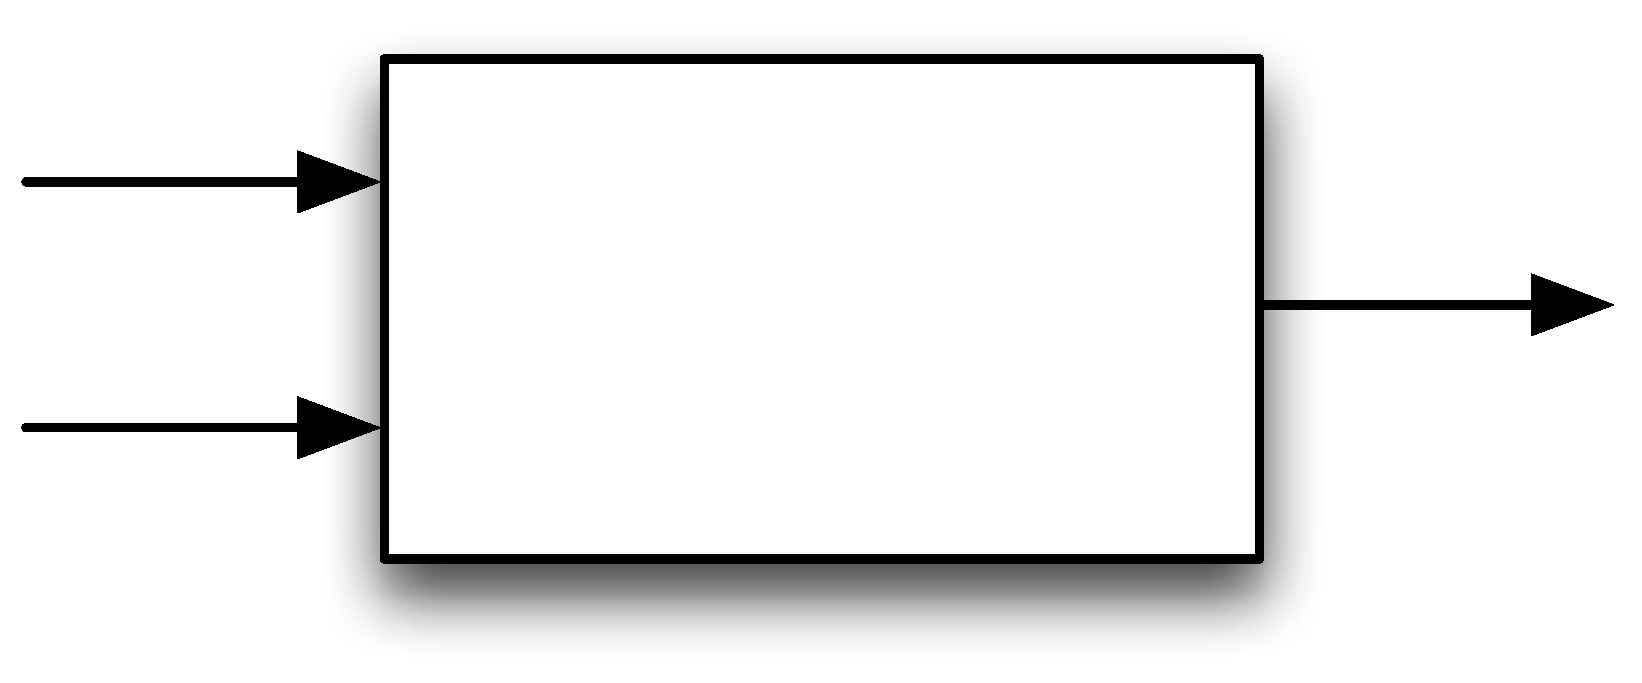
\includegraphics[width=2.5in]{Pictures/functionPic.pdf}
\end{center} 
The function gives an \textbf{output}\index{output} value which depends upon 
the \textbf{input}\index{input} value(s).
We will often also use the term {\bf result}\index{result}
for the output, and the terms {\bf arguments} or\index{argument}
{\bf parameters}\index{parameter} for the inputs. 

A simple example of a function is addition, \texttt{+}, over numbers.
Given input values \texttt{12} and \texttt{34} the corresponding output will be 
\texttt{46}.
\begin{center}
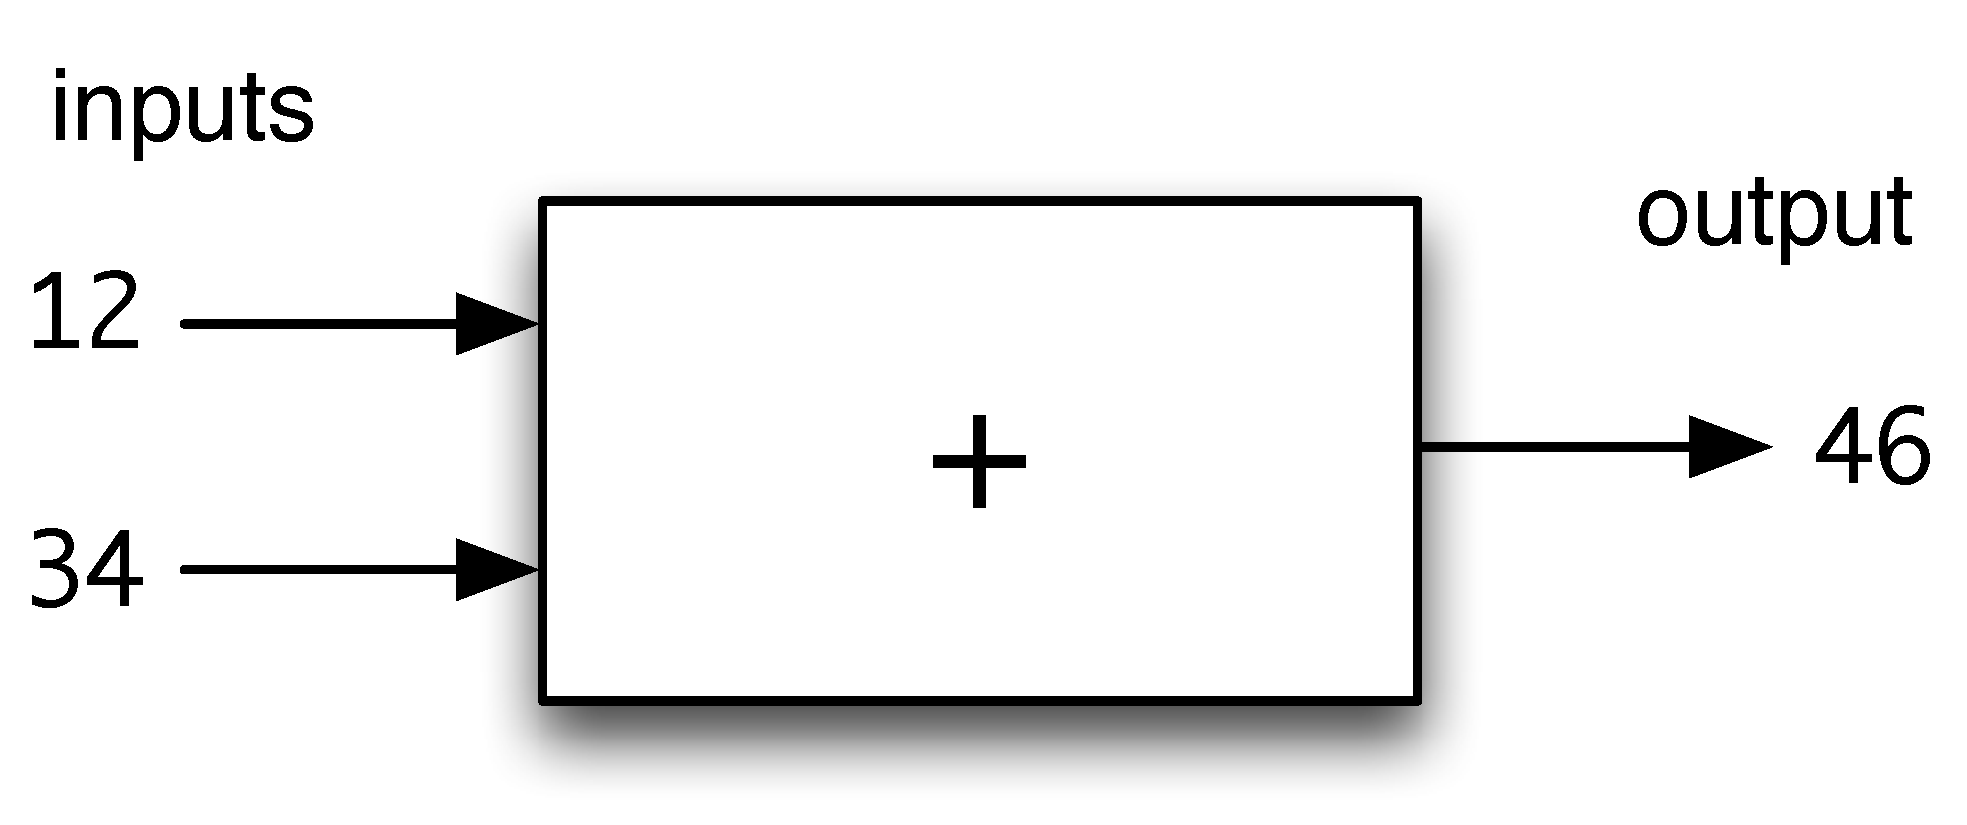
\includegraphics[width=3.0in]{Pictures/addFunPic.pdf}
\index{addition!function diagram}
\end{center} 
The process of giving particular inputs to a function is called \textbf{function
application}\index{application|see{function application}}\index{function application}, and
\texttt{(12 + 34)} represents the application of the function \texttt{+}\minx{+} to
\texttt{12} and \texttt{34}.

Addition is a mathematical example, but there are also functions in
many other situations; examples of these include
\label{examples1}  
\begin{titemize}
\item a function giving the distance by road ({\em output}) between two cities
({\em inputs});
\item a supermarket check-out program, which calculates the bill
({\em output}) from a list of bar codes scanned in ({\em input}); and
\item a process controller, which
controls valves in a chemical plant. Its inputs are the information from
sensors, and its output the signals sent to the valve actuators.
\end{titemize}
Different paradigms are characterized by the different tools
which they provide for modelling. In a functional programming language we'll focus on values -- such as bar codes and bills -- and the functions which work over them -- giving the total of a bill, say. We'll also see this
in our running example of pictures, which we look at next.

\section{Pictures and functions}
\label{picturesFuns}
\index{case studies!pictures|see{pictures}}
\index{pictures|(}


Let's take our first look at how pictures might be modelled.
First of all, we want to show that many common
relationships between pictures are modelled by functions; in the remainder of 
this section we consider a series of examples of this.

Reflection in a vertical mirror will relate two pictures, and we
can model this by a function \texttt{flipV}:\minx{flipV}
\begin{center}
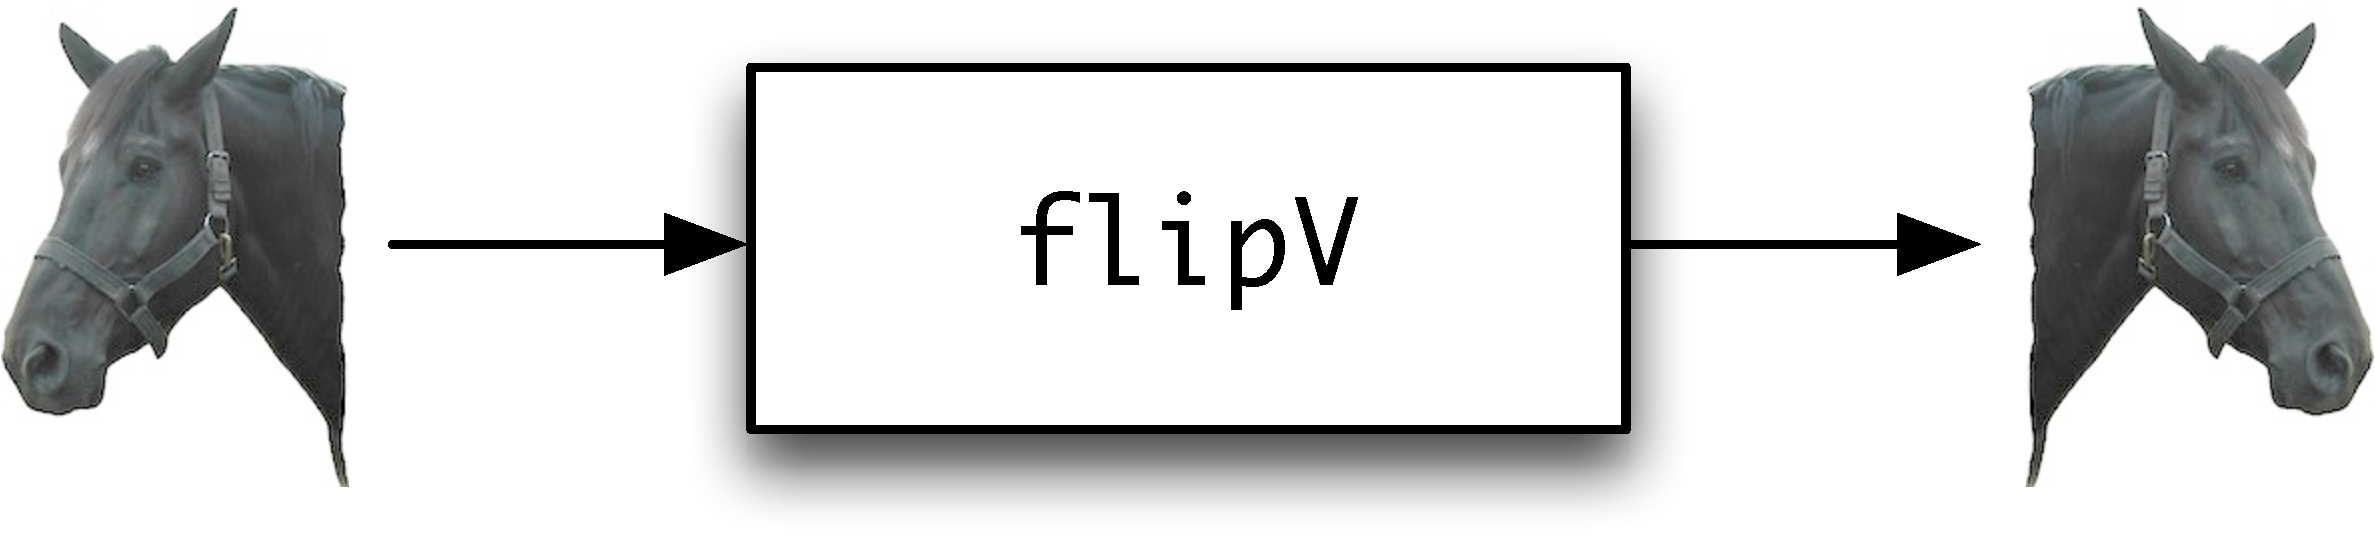
\includegraphics[width=3.5in]{Pictures/flipV.pdf}
\end{center}
where we have illustrated the effect of this reflection on the `horse'
image.
In a similar way we have a function \texttt{flipH} to represent flipping in a
horizontal mirror. 
Another function models the
inversion of the colours in a (monochrome) image:
\begin{center}\minx{invertColour}
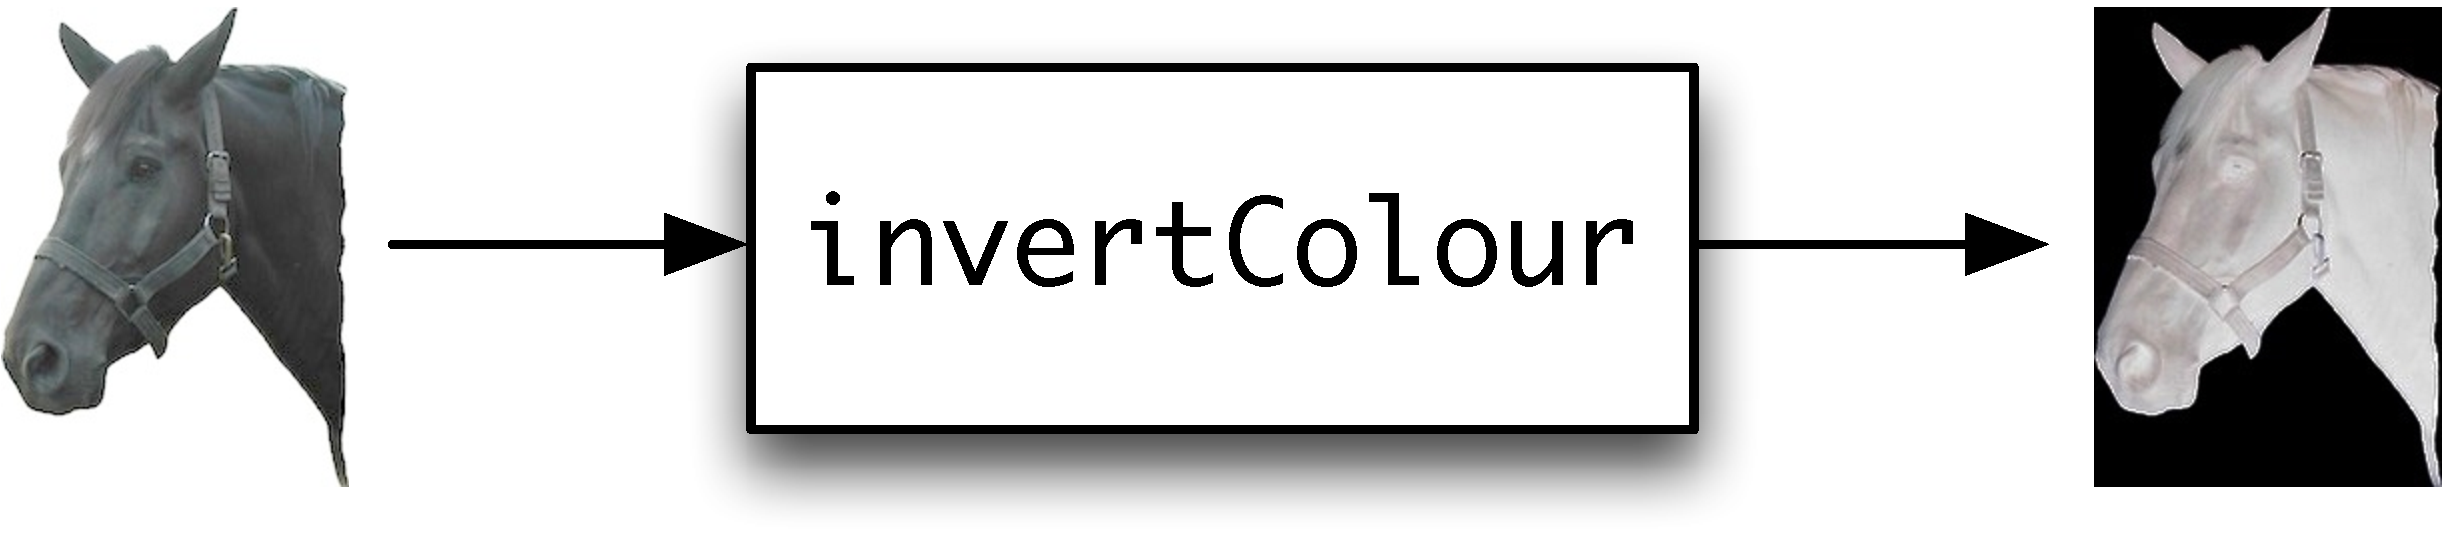
\includegraphics[width=3.8in]{Pictures/reverseVideo.pdf}
\end{center}
Some functions will take two arguments, among them a function to scale
images,
\begin{center}\index{scale@\texttt{scale}}
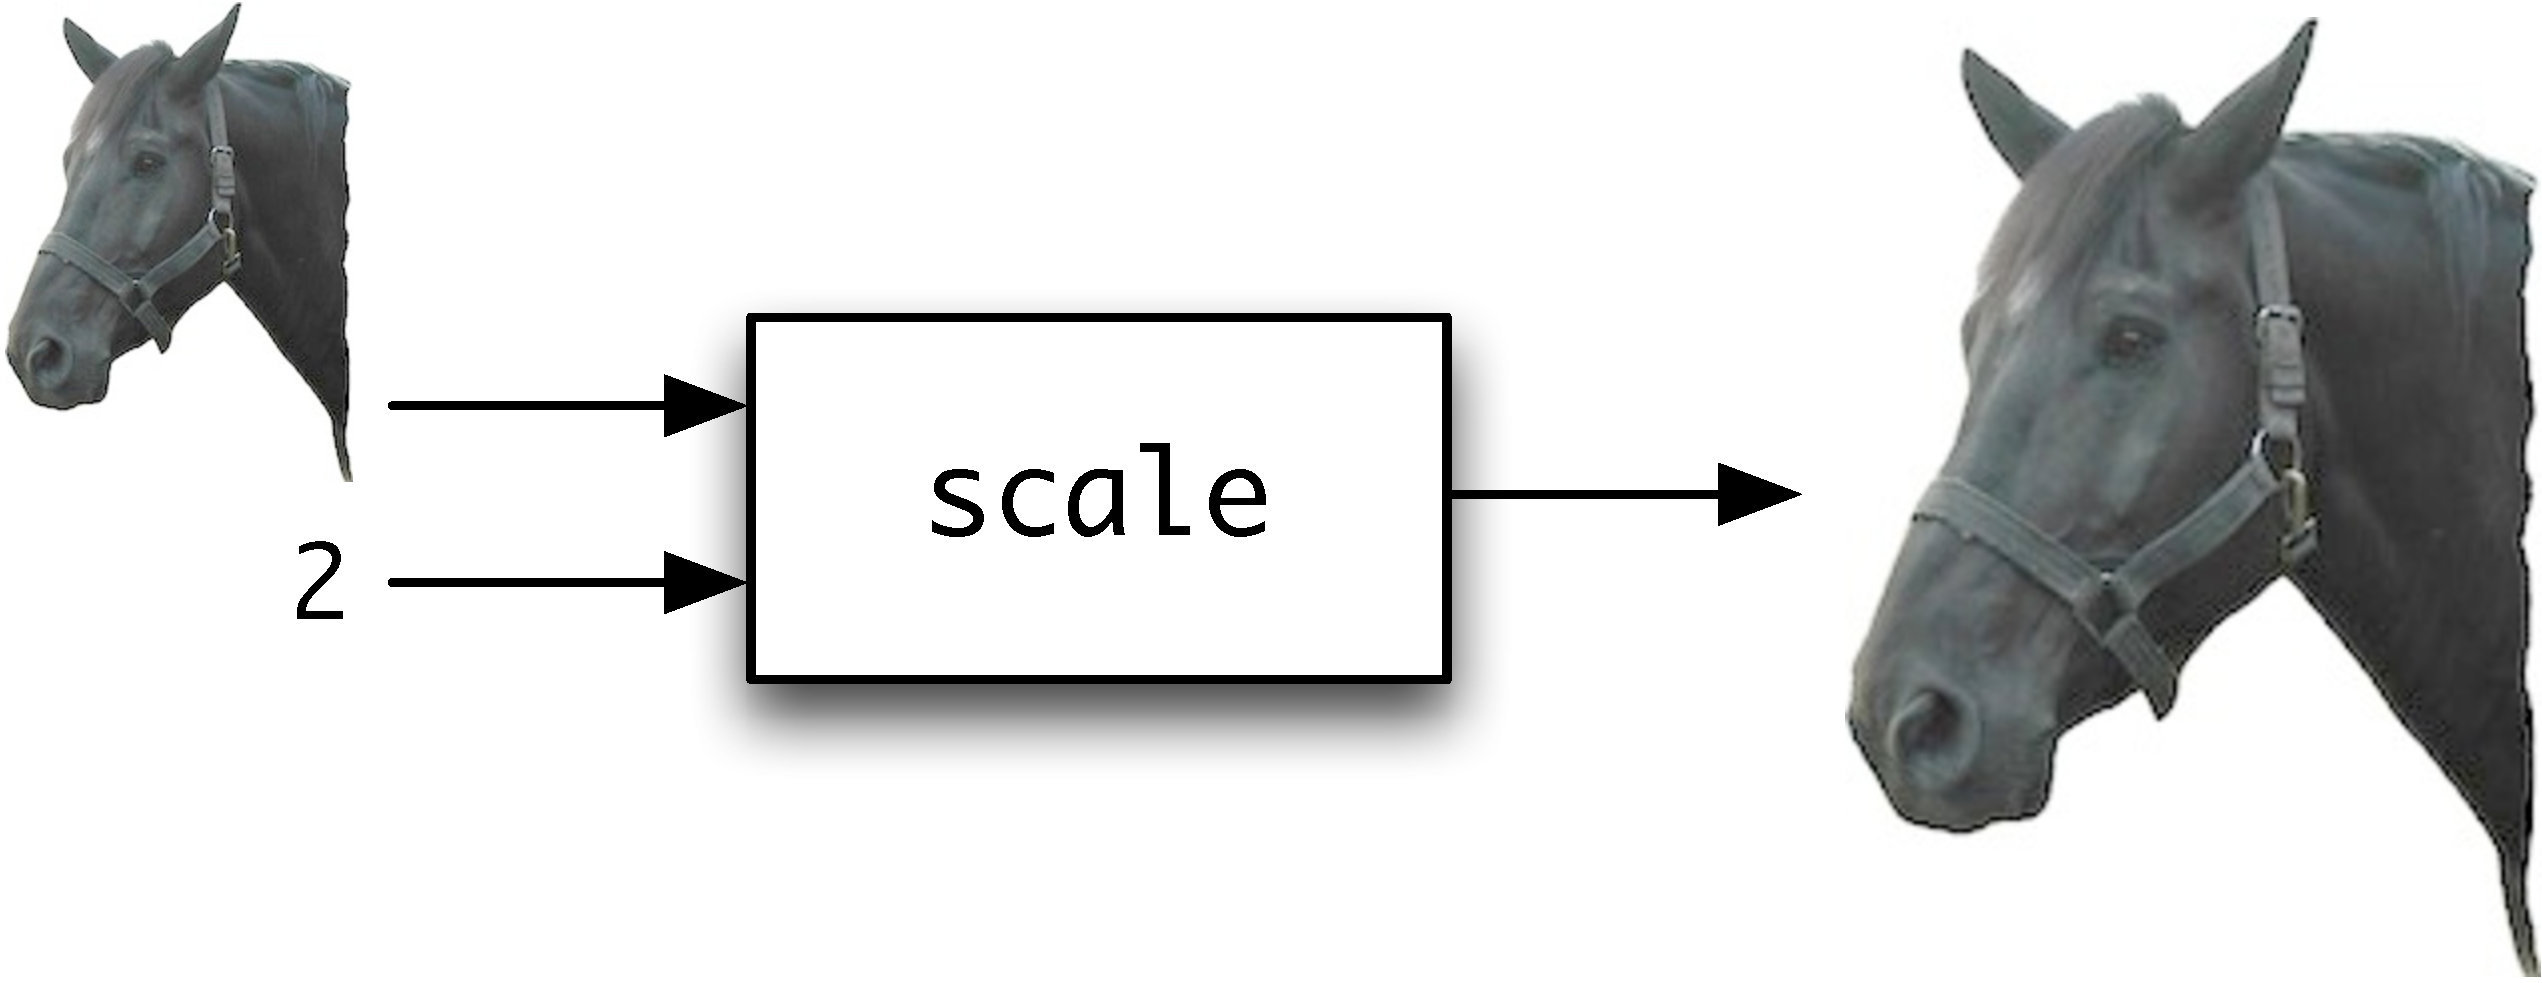
\includegraphics[width=3.8in]{Pictures/scale2.pdf}
\end{center}
a function to put one picture above another,
\begin{center}\minx{above}
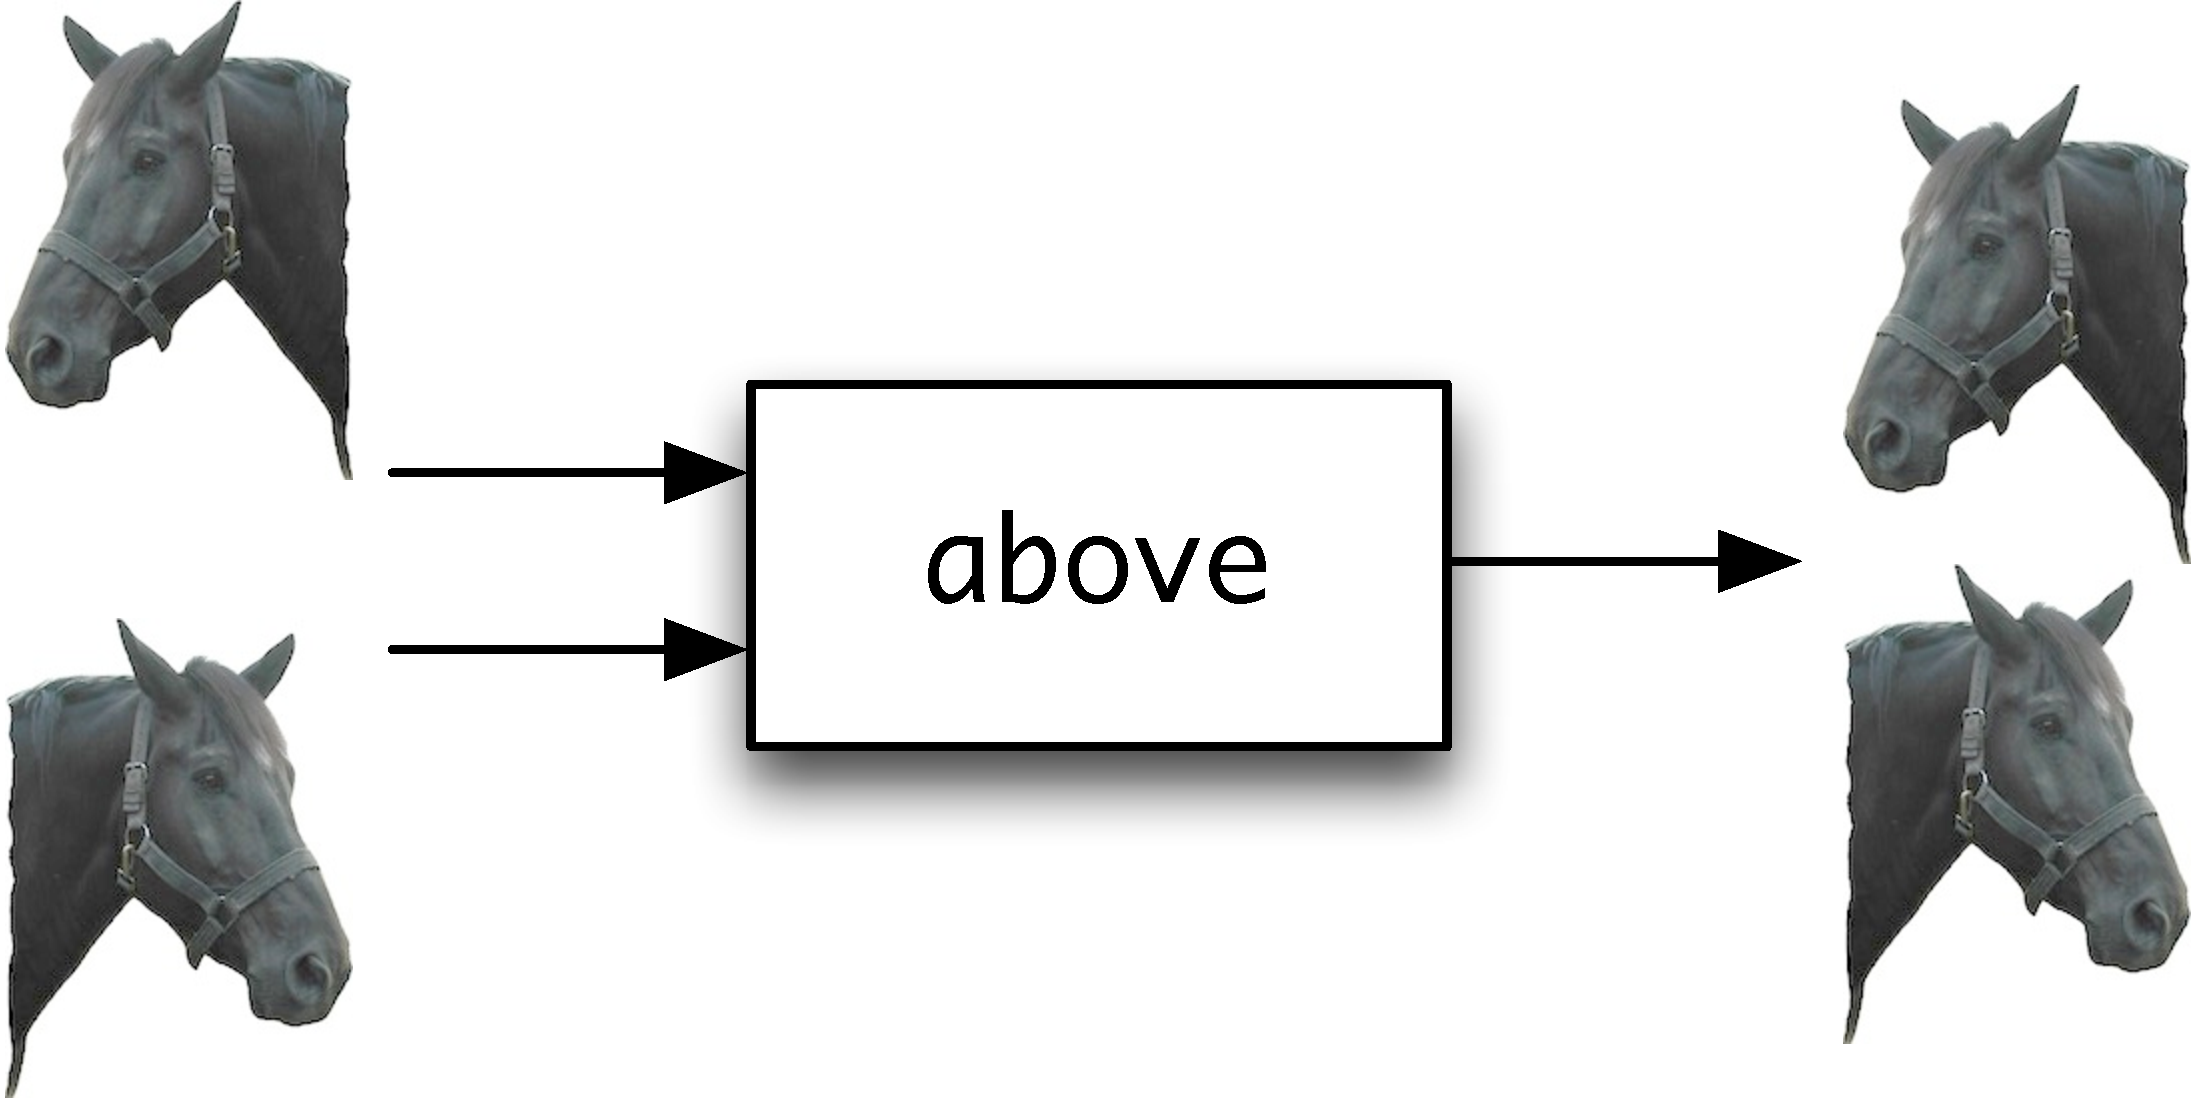
\includegraphics[width=3.4in]{Pictures/above.pdf}
\end{center}
and a function to place two pictures side by side.
\begin{center}\minx{beside}
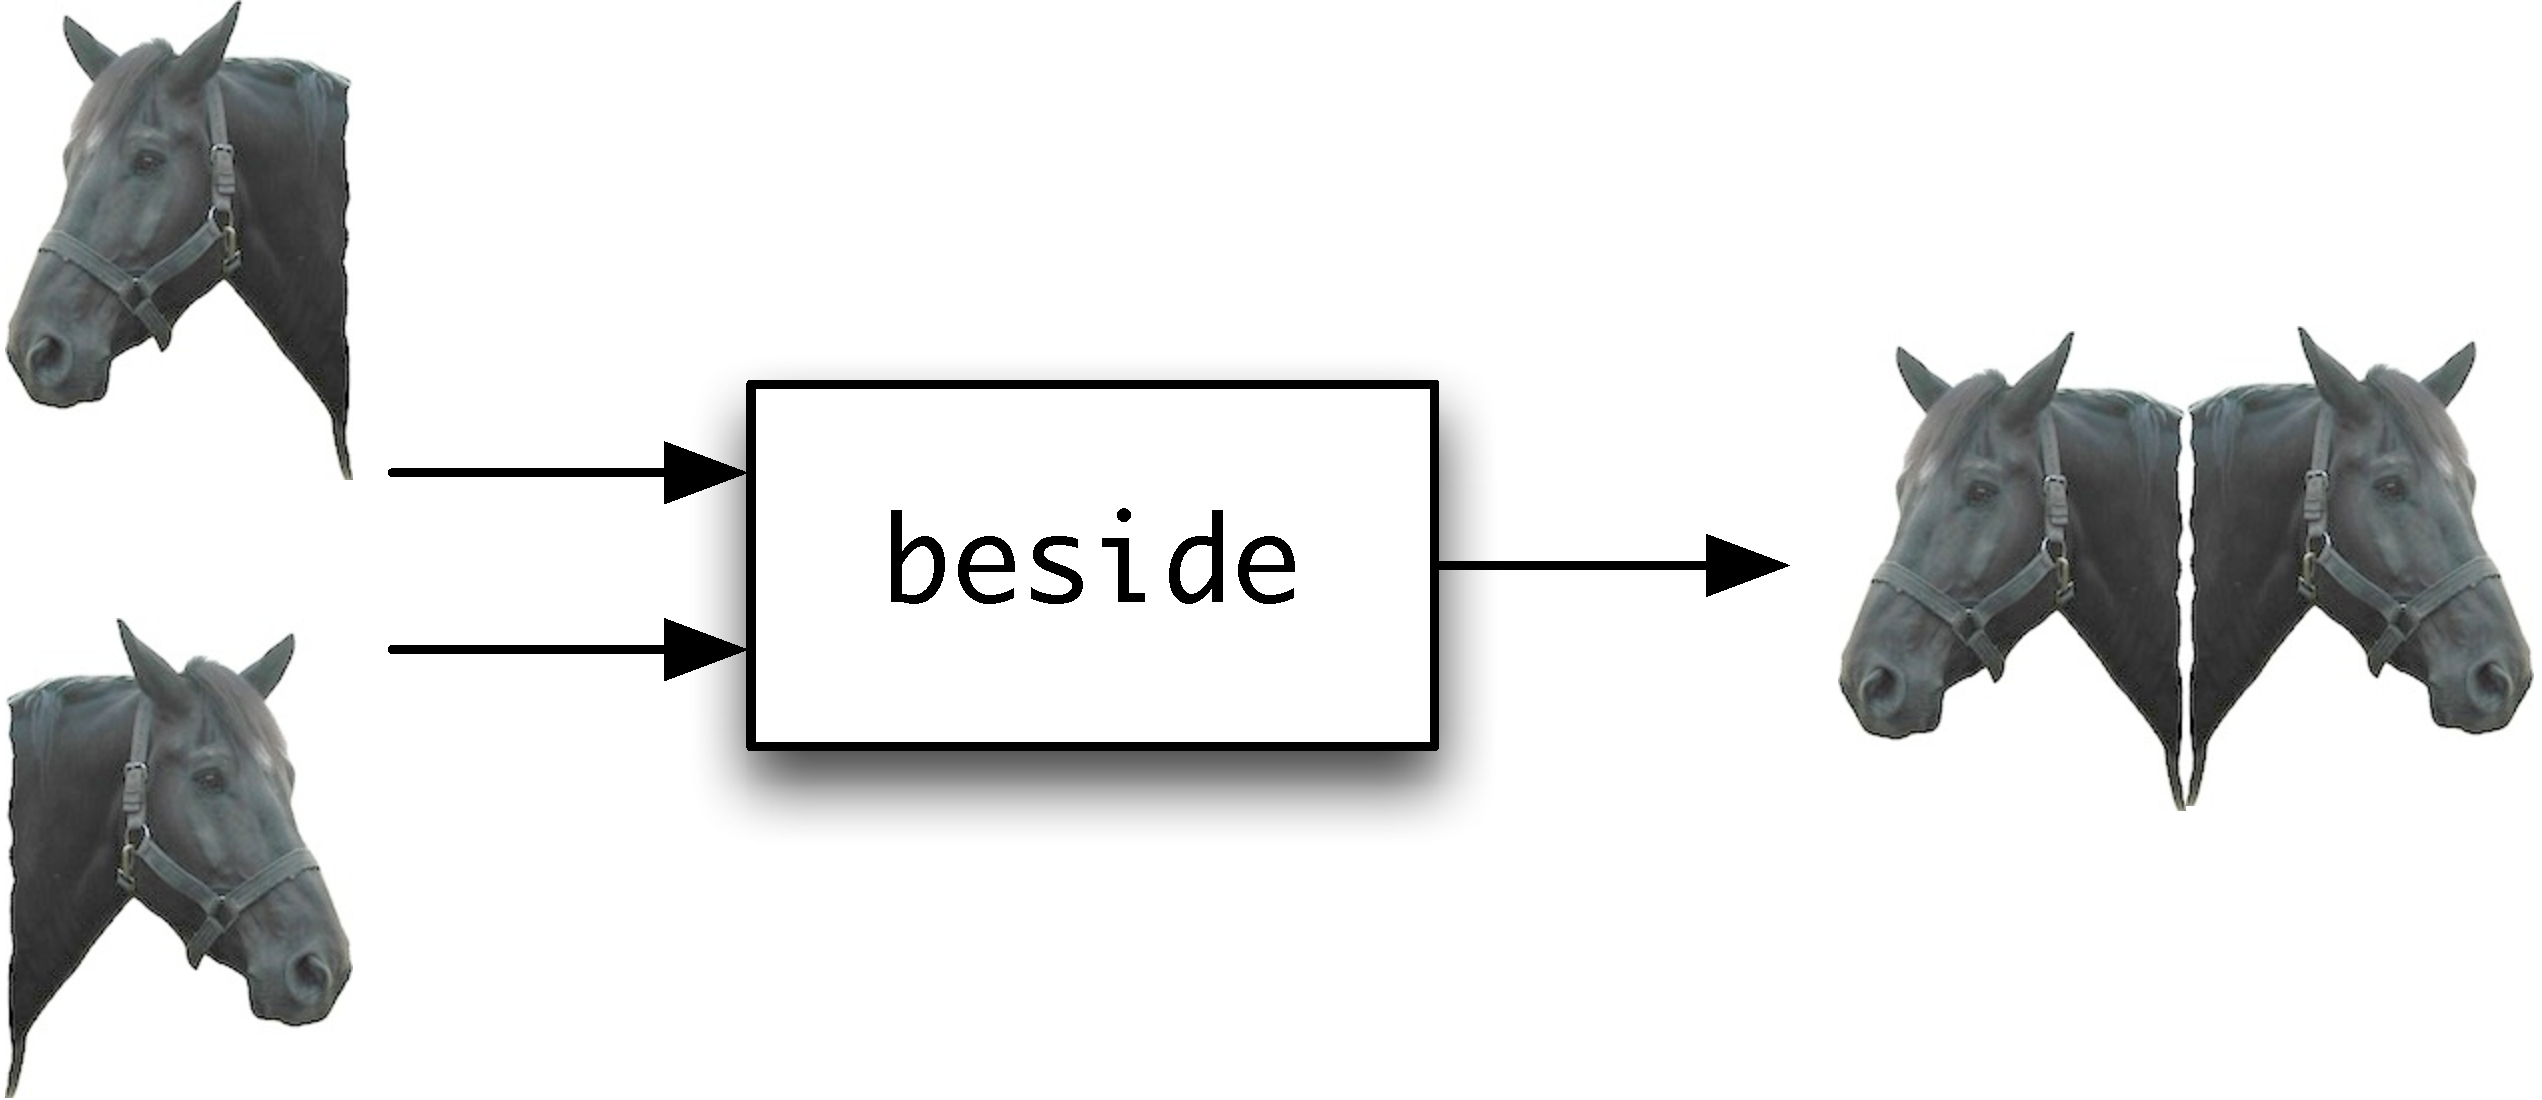
\includegraphics[width=3.8in]{Pictures/sideBySide.pdf}
\end{center}
All the functions here show that functions take a number of inputs (or arguments, parameters) and produce an output (or result) that depends on those inputs. What's more, this result only depends on those inputs, and will always give the same result for the same inputs. 

Before we can fully explain functional programming in Haskell, we
have to explain types, which we do now.

\section{Types}
\index{type}\label{typesIntro}

The functions which we use in functional programs will involve all sorts of
different kinds of value: the addition function \texttt{+} will combine two
numbers to give another number; \texttt{flipV}\minx{flipV} will transform a picture
into a picture; \texttt{scale}\index{scale@\texttt{scale}} will take a picture and a number and
return a picture, and so on. 

A \textbf{type}\index{type} is a collection of values, such as numbers
or pictures, grouped together because although they are different --
\texttt{2} is not the same as \texttt{567} -- they are the same {\em sort\/} of thing, in
that we can do the same things to them. In particular, we can apply the same functions to them.  For instance, we can find the larger
of any two numbers, but it doesn't make sense to do this for two pictures or a number and a picture. 
 
Each of the functions we have looked at so far will accept inputs from particular types, and give a result of a particular type too. If we look at the addition function, \texttt{+}, it only makes sense to add two scnumbers
but not two pictures, say. 
This is an example of the fact that the functions we have been talking about
themselves have a type, and indeed we can illustrate this diagrammatically:
\begin{center}\minx{+}\minx{Int}
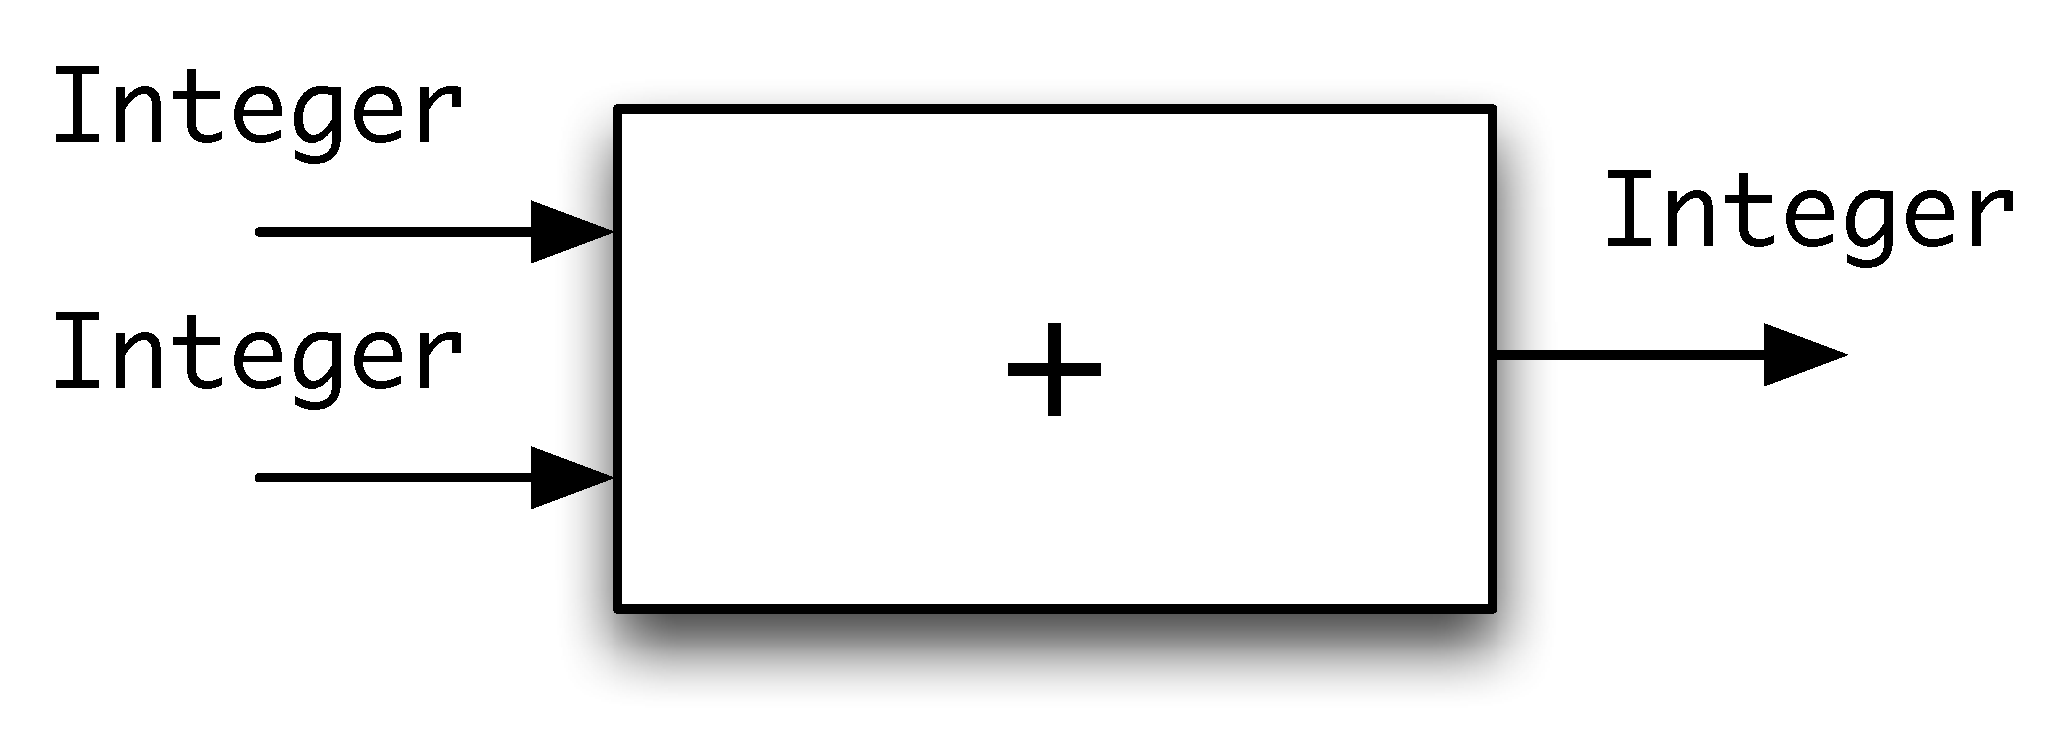
\includegraphics[width=3.0in]{Pictures/addFunPic2.pdf}\end{center}
\index{addition!type diagram}
The diagram indicates that \texttt{+} takes two whole numbers (or
\texttt{Integers})\minx{Integer} as arguments and gives an \texttt{Integer} as a result. In
a similar way, we can label the \texttt{scale} function
\begin{center}\index{scale@\texttt{scale}}
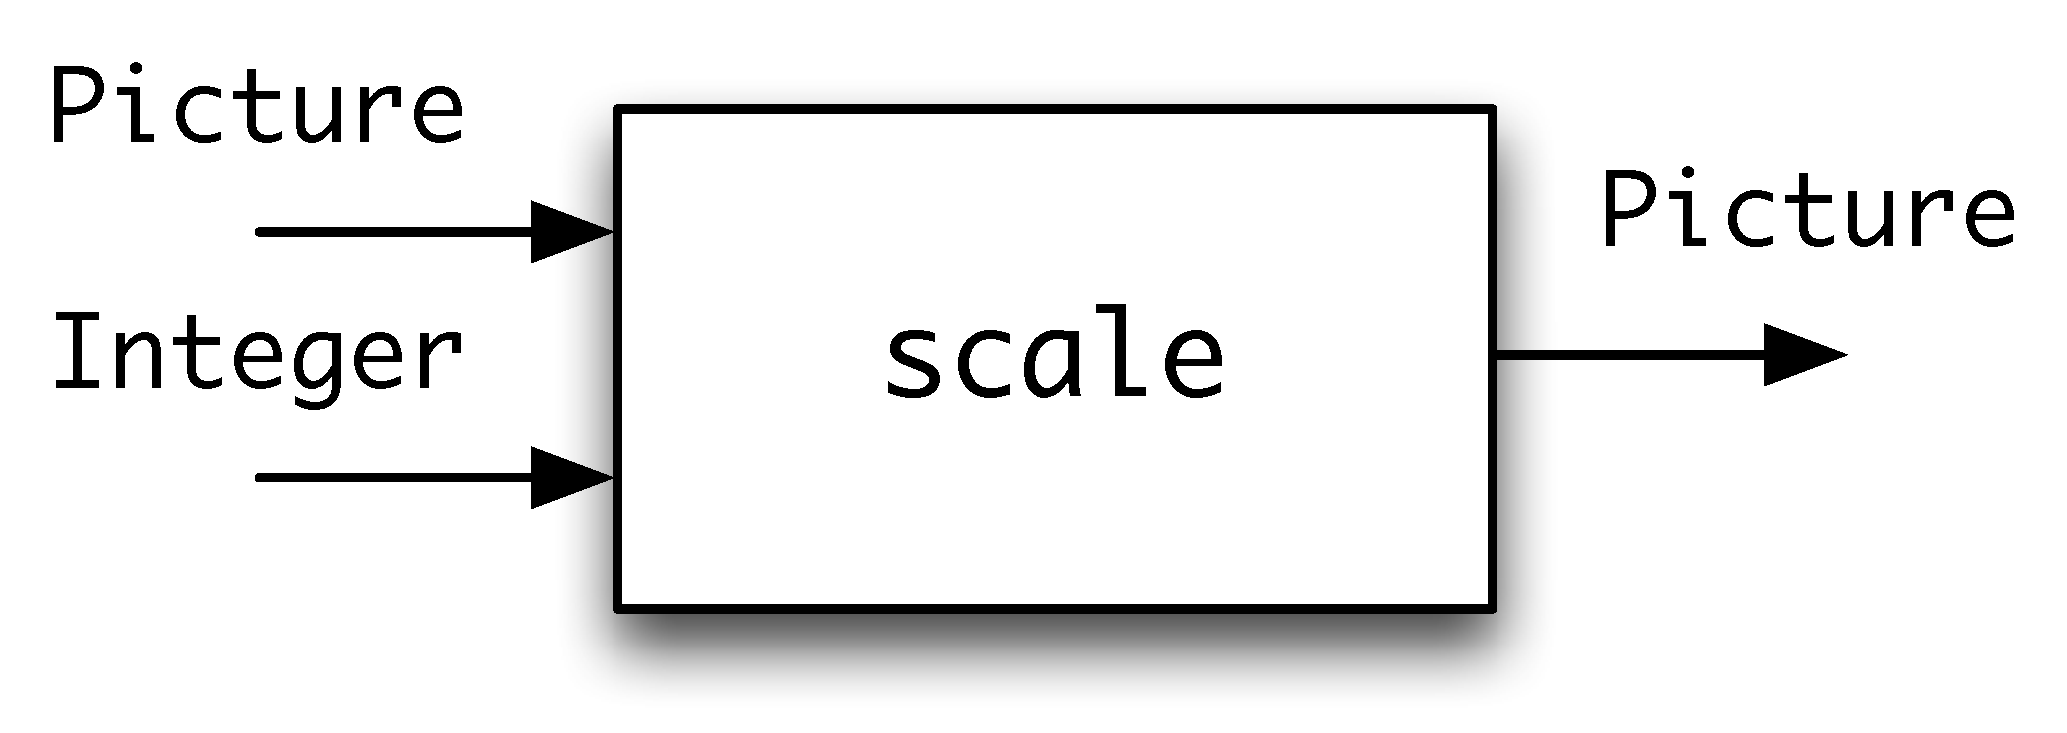
\includegraphics[width=3.0in]{Pictures/scaleType.pdf}
\end{center}\index{scale@\texttt{scale}!type diagram}
to indicate that its first argument is a \texttt{Picture}\minx{Picture} and its second
is an \texttt{Integer}, with its result being a \texttt{Picture}. We can see an example of this here, where \texttt{above} is correctly applied to two \texttt{Pictures}
\begin{center}\minx{above}
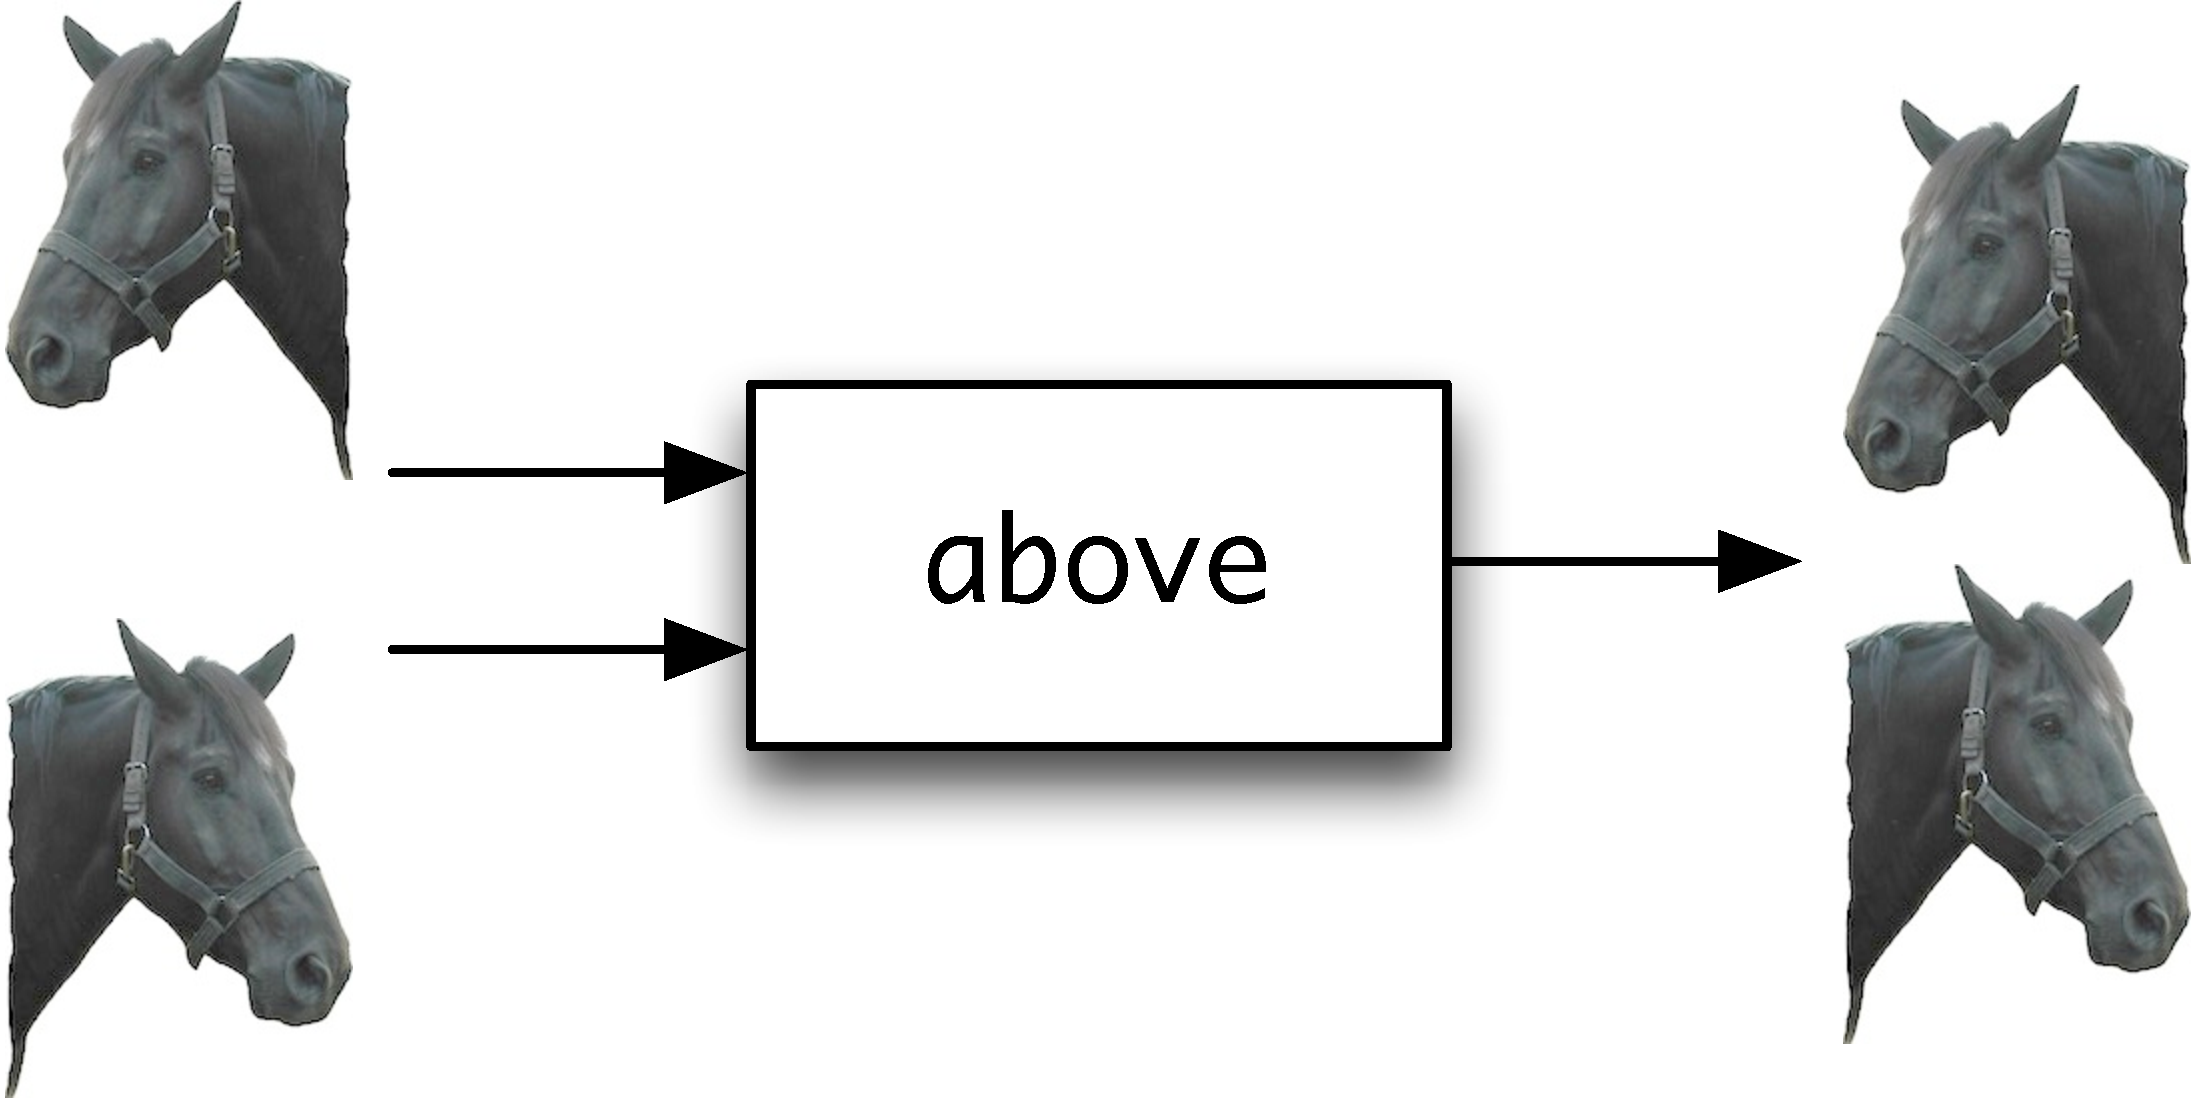
\includegraphics[width=3.4in]{Pictures/above.pdf}
\end{center}
but when applied to a \texttt{Picture} and an \texttt{Integer} a \textbf{type error} occurs, indicating that we have made a mistake:
\begin{center}\minx{above}
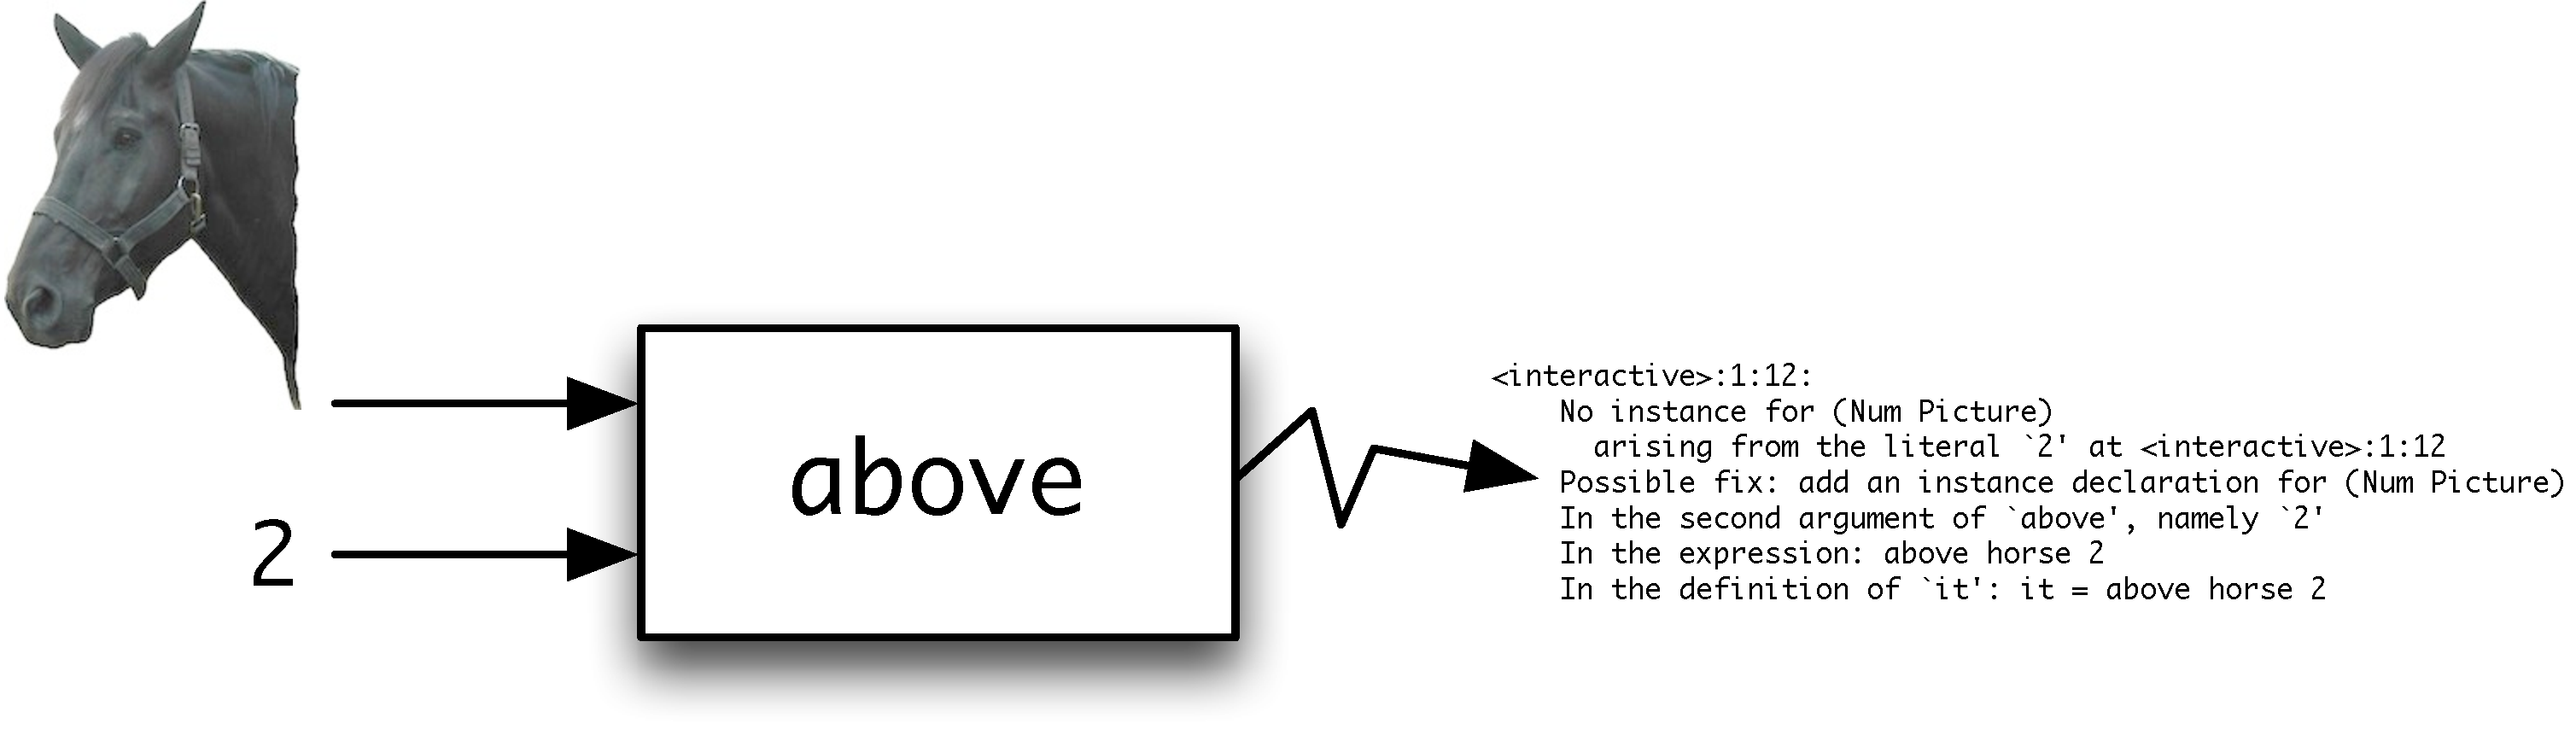
\includegraphics[width=5.0in]{Pictures/aboveError.pdf}
\end{center}
We have now explained two of the central ideas in functional
programming: a type is a collection of values, like the whole numbers or
integers; a function
is an operation\index{operation} which takes one or more
arguments to produce a result. The two concepts are linked: functions will operate over 
particular types:
a function to scale a picture will take two arguments, one of type \texttt{Picture} and
the other of type \texttt{Int}, and return a \texttt{Picture}. 

In modelling a
problem situation -- often called a problem \textbf{domain}\index{domain} -- types represent the things\footnote{I have not used the word `object' here because that has a technical meaning in OO languages; you could use it, but just remember it's meant in the non-technical sense here.} in the domain, while functions will represent what can be done to transform or manipulate the objects. In the case of pictures, we'll have a type \texttt{Picture} to represent the pictures themselves, and functions give operations on pictures, such as placing one above another, or scaling a picture. 

A rough and ready rule is that types correspond to \emph{nouns}, while functions, which transform or combine values from these types, are like \emph{verbs}. We come back to types in Section
\ref{typesFP} below.
\index{pictures|)}


\section{The Haskell programming language}


Haskell\index{Haskell} \cite{haskell2010} is the particular functional programming language which
we use in this text. Haskell was first defined in 1990, and it has undergone a series of changes since then: the version as I write is Haskell 2010.

Haskell is named after Haskell B.\ Curry,\index{Curry, Haskell B.} who was one of the pioneers of
the $\lambda$ calculus (lambda calculus)\index{lambda calculus},
a mathematical theory of functions that has been an
inspiration to designers of a number of functional languages. 

The best place to find out about everything to do with Haskell -- including the language definition itself, implementations, libraries, resources, mailing lists, news and Haskell jobs -- is the \texttt{haskell.org} website:
\begin{center}
\index{Web site!for Haskell}\index{haskell.org}
\url{https://www.haskell.org/}
\end{center}
There are various implementations of Haskell; in this 
text we shall use \textbf{GHCi}\index{GHCi} \citeyear{GHCi}. `GHCi' is an abbreviation for `Glasgow Haskell Compiler interactive': work on the compiler was started when Simon Peyton Jones and Simon Marlow were at Glasgow University; they are now both at Microsoft  Research in Cambridge.
GHCi provides an excellent environment for the learner, since it is freely
available for PC, Linux and Mac OS X systems, it is efficient and compact
and has a flexible user interface.

GHCi is an interpreter\index{interpreter} -- which means loosely that 
it evaluates expressions step-by-step as we might on a piece of paper -- but it can also load code that has been compiled into machine language. So, GHCi combines the flexibility of an interpreter with the efficiency of a compiler,\index{compiler} 
allowing its programs to run with a speed similar to those
written in more conventional languages like C and C++. Details of other
different implementations of Haskell can be found in Appendix
\ref{OtherHS}, and a full description of all of them is available at the \texttt{haskell.org} page.


GHCi is installed, together with the \textbf{Cabal}\index{Cabal} \cite{Cabal} build tool, using \textbf{GHCup}\index{GHCup}, \url{https://www.haskell.org/ghcup/}, the toolchain installer that \texttt{haskell.org} itself recommends; we describe how to install it in Chapter \ref{getStart}. Libraries beyond those that come with GHC are available from an extensive online database, \textbf{HackageDB}\index{HackageDB} \cite{Hackage}, and Cabal makes it easy to download and install them: we describe how to work with the interactive version of GHC in the next chapter, and how to use Hackage and Cabal in Chapter \ref{progLists}.

All the programs and examples used in the text can be downloaded as the \texttt{Craft3e} package from Cabal and from the website for this book,
\begin{center}
\label{bookWeb}
\url{http://www.haskellcraft.com/}
\end{center}\minx{www.haskellcraft.com}\index{website}
This site also pulls together a collection of resources, further reading and other background materials for this text.

\section{Expressions and evaluation}
\label{exprEval}

In our first years at school we learn to \textbf{evaluate}\index{evaluation}
an \textbf{expression}\index{expression} like \texttt{(7 - 3) * 2}
\begin{center}
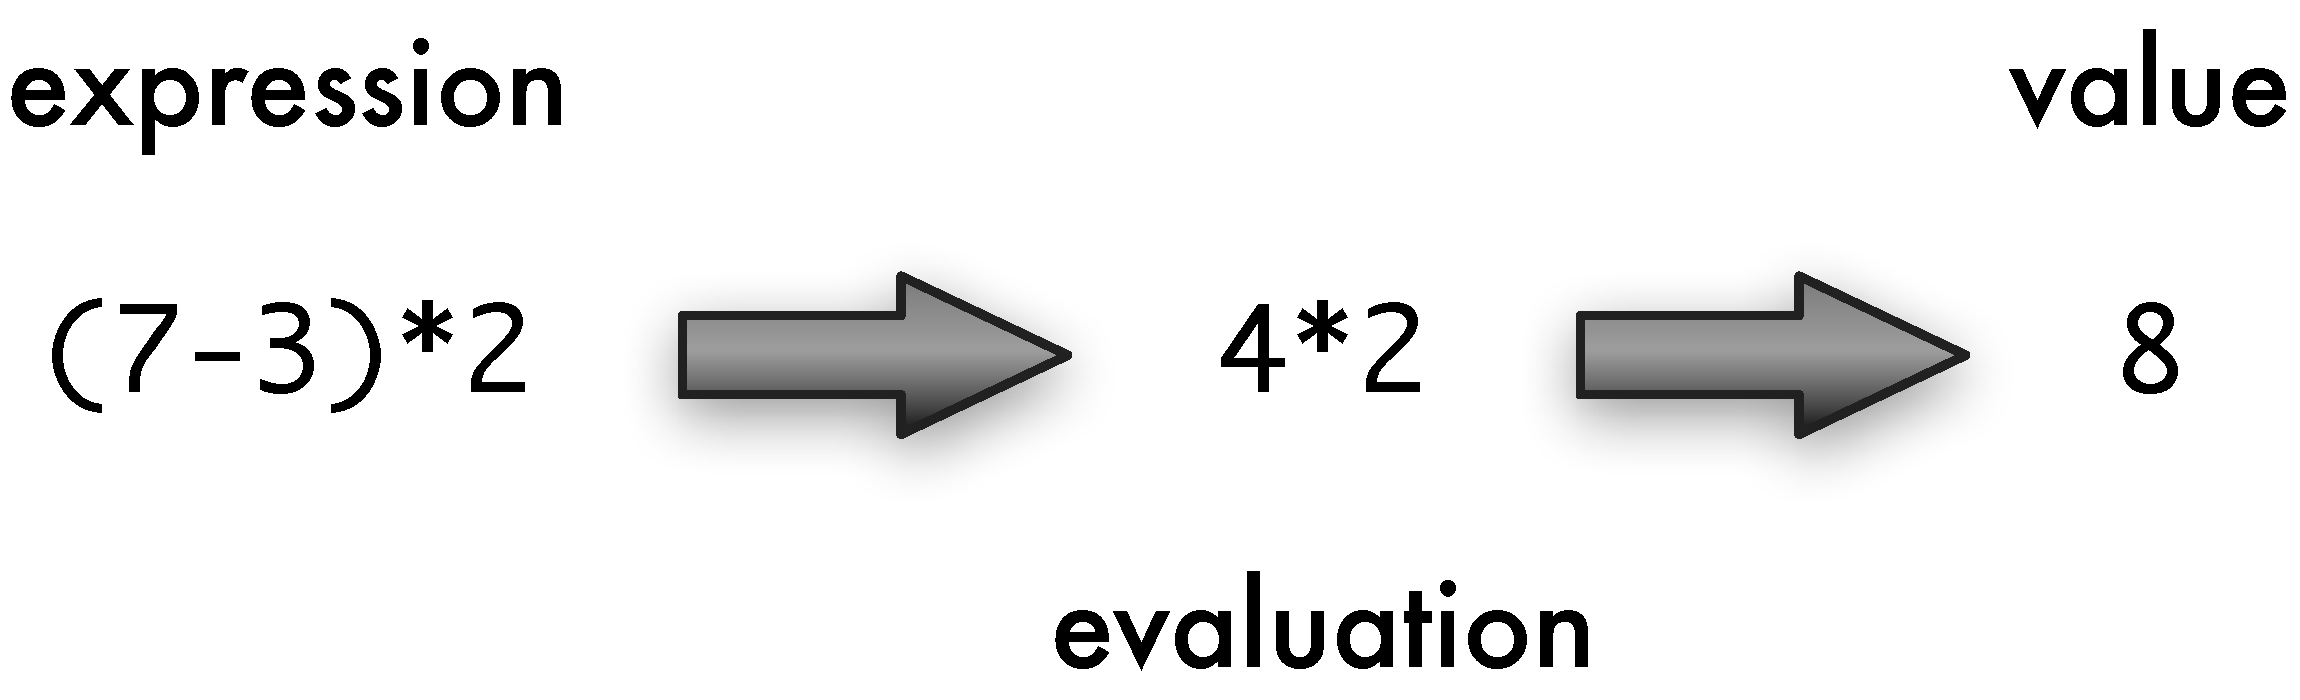
\includegraphics[width=3in]{Pictures/evaluation.pdf}
\end{center}
to give the \textbf{value}\index{value} \texttt{8}.
Expressions are built up by applying functions to numbers and other expressions built in the same way. In this particular example, the functions are subtraction \texttt{-}\minx{-} and multiplication \minx{*}\texttt{*}, and the numbers \texttt{7}, \texttt{3} and \texttt{2}; the value of the expression is a number.
This process of evaluation is automated in an electronic calculator.

In functional programming we do exactly the same: we evaluate expressions
to give values, but in those expressions we use functions which
model our particular problem. For example, in modelling pictures we will want
\index{pictures}
to evaluate expressions whose values are pictures.
If the picture\minx{horse}
\begin{center}
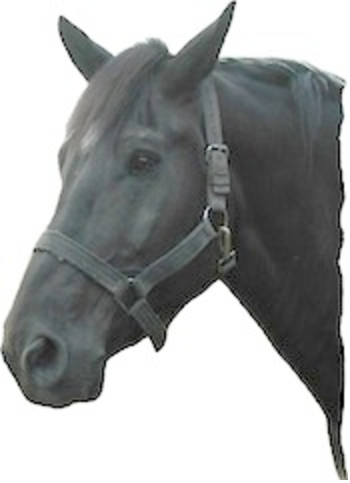
\includegraphics[width=0.6in]{Pictures/simplePic.pdf}
\end{center}
is called \texttt{horse}, then we can form an expression by applying the
function \texttt{flipV}\minx{flipV} to the horse. This function
application\index{function application} is written by putting the function
followed by its arguments, like this:
\begin{alltt}
flipV horse
\end{alltt}
and then evaluation will give
\begin{center}
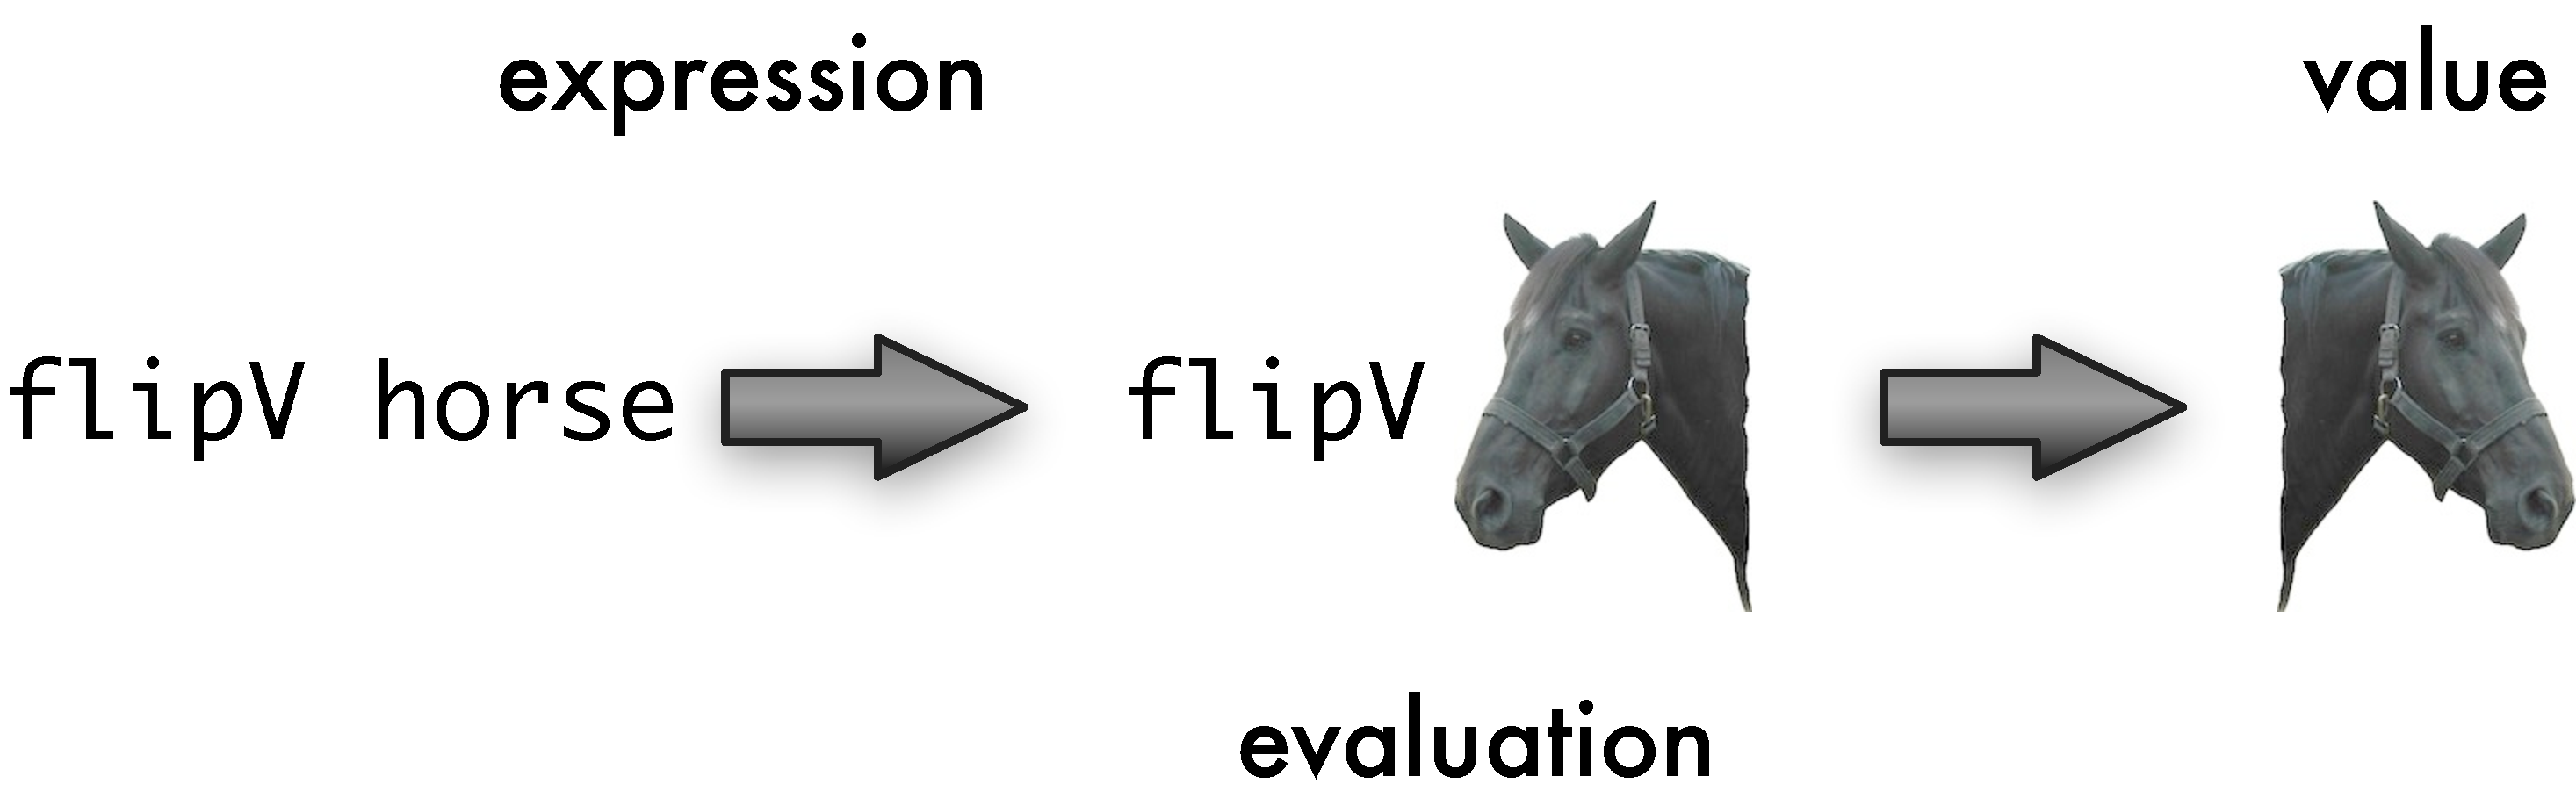
\includegraphics[width=3.8in]{Pictures/evaluation2.pdf}
\end{center}
A more complicated expression is
\begin{alltt}\minx{invertColour}
invertColour (flipV horse)
\end{alltt}
the effect of which is to give a horse reflected in a
vertical mirror -- \texttt{flipV horse} as shown above -- and then to invert
the colours in the picture to give
\begin{center}
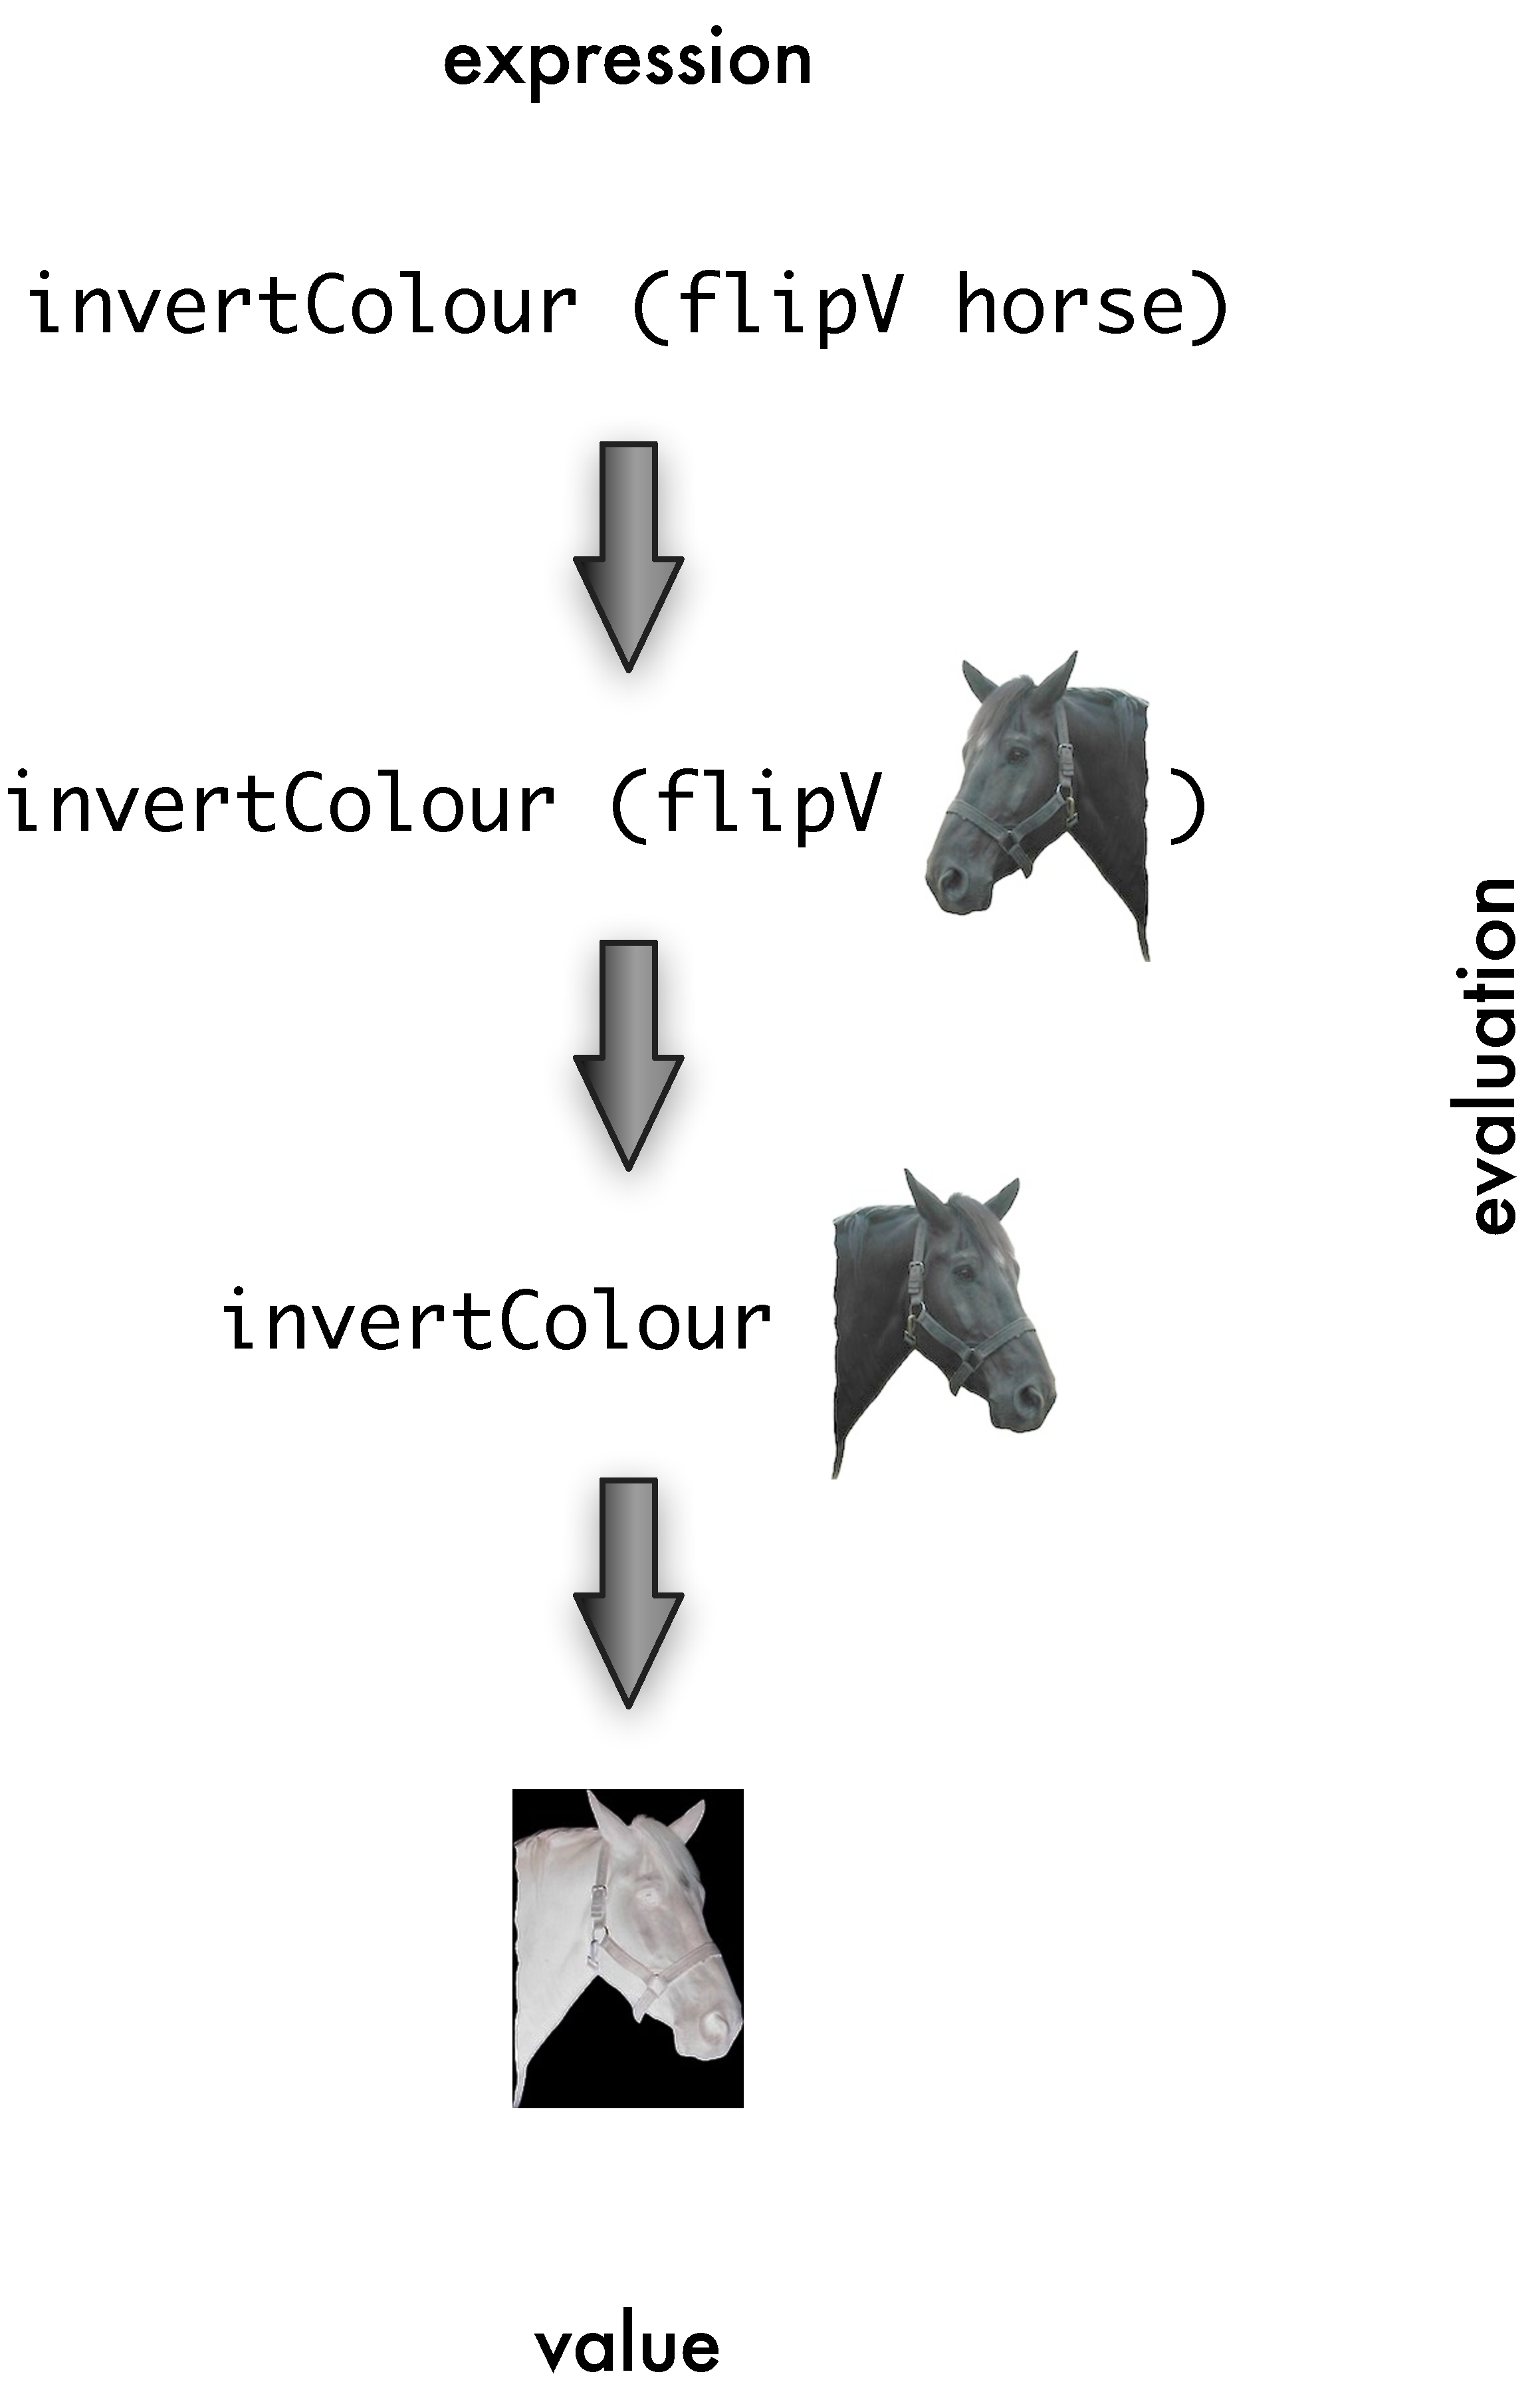
\includegraphics[width=2.8in]{Pictures/evaluation3.pdf}
\end{center}
To recap, in functional programming, we compute by evaluating
expressions which use functions in our area of interest. We can see an implementation of 
a functional language as something like an electronic calculator: we
supply an expression, and the system evaluates the expression to give
its value. The task of the programmer is to write the functions which
model the problem area.

So, a \textbf{functional
program}\index{functional program} is made up of a series of
\textbf{definitions}\index{definition} of functions and other values. 
We will look at how to write these definitions now.


\section{Definitions}
\label{defsIntro}

A functional program in Haskell consists of a number of
\textbf{definitions}\index{definition}. A Haskell
definition associates a \textbf{name}\index{name}
with a value of a particular \textbf{type}. 
We often use the word `\textbf{identifier}'\index{identifier} instead of `name': they mean exactly the same thing.

In the simplest
case a definition will look like this\minx{=}
\begin{alltt}
name :: type
name = expression
\end{alltt}
as in the example
\begin{alltt}
size :: Integer
size = 12+13
\end{alltt}
which associates the name on the left-hand side, \texttt{size}, with the value of the expression
on the right-hand side, \texttt{25}, a value whose type is \texttt{Integer}\minx{Integer}, the type of whole numbers
or integers. The symbol `\texttt{::}'\minx{::} can be read as ``is a / is an'', so the first line of the last definition reads `\texttt{size} is an \texttt{Integer}'.\index{reading `\texttt{::}'} Note also that names for functions and other
values begin with a \emph{small letter}, while type names begin with a \emph{capital
letter}.\index{name!value}\index{name!type}



Suppose that we are supplied with the definitions of \texttt{horse} and the various
functions over \texttt{Picture}\minx{Picture} mentioned earlier -- we will discuss in 
detail how to download these and use them in a program in Chapter \ref{getStart} -- we can
then
write definitions which use these operations over pictures. For example, we can say
\begin{alltt}\minx{blackHorse}
blackHorse :: Picture
blackHorse = invertColour horse
\end{alltt}
so that the \texttt{Picture} associated with \texttt{blackHorse} is obtained by
applying the function \texttt{invertColour} to the \texttt{horse},
thus giving
\begin{center}
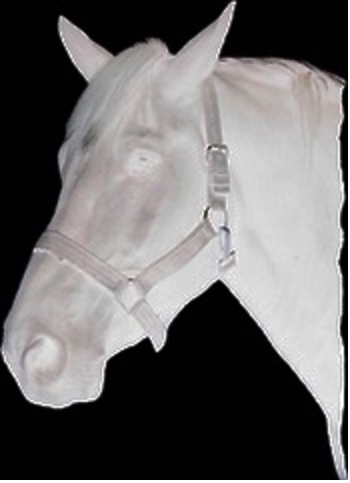
\includegraphics[width=0.6in]{Pictures/blackHorse.pdf}
\end{center}

\begin{figure}[t]
\begin{center}
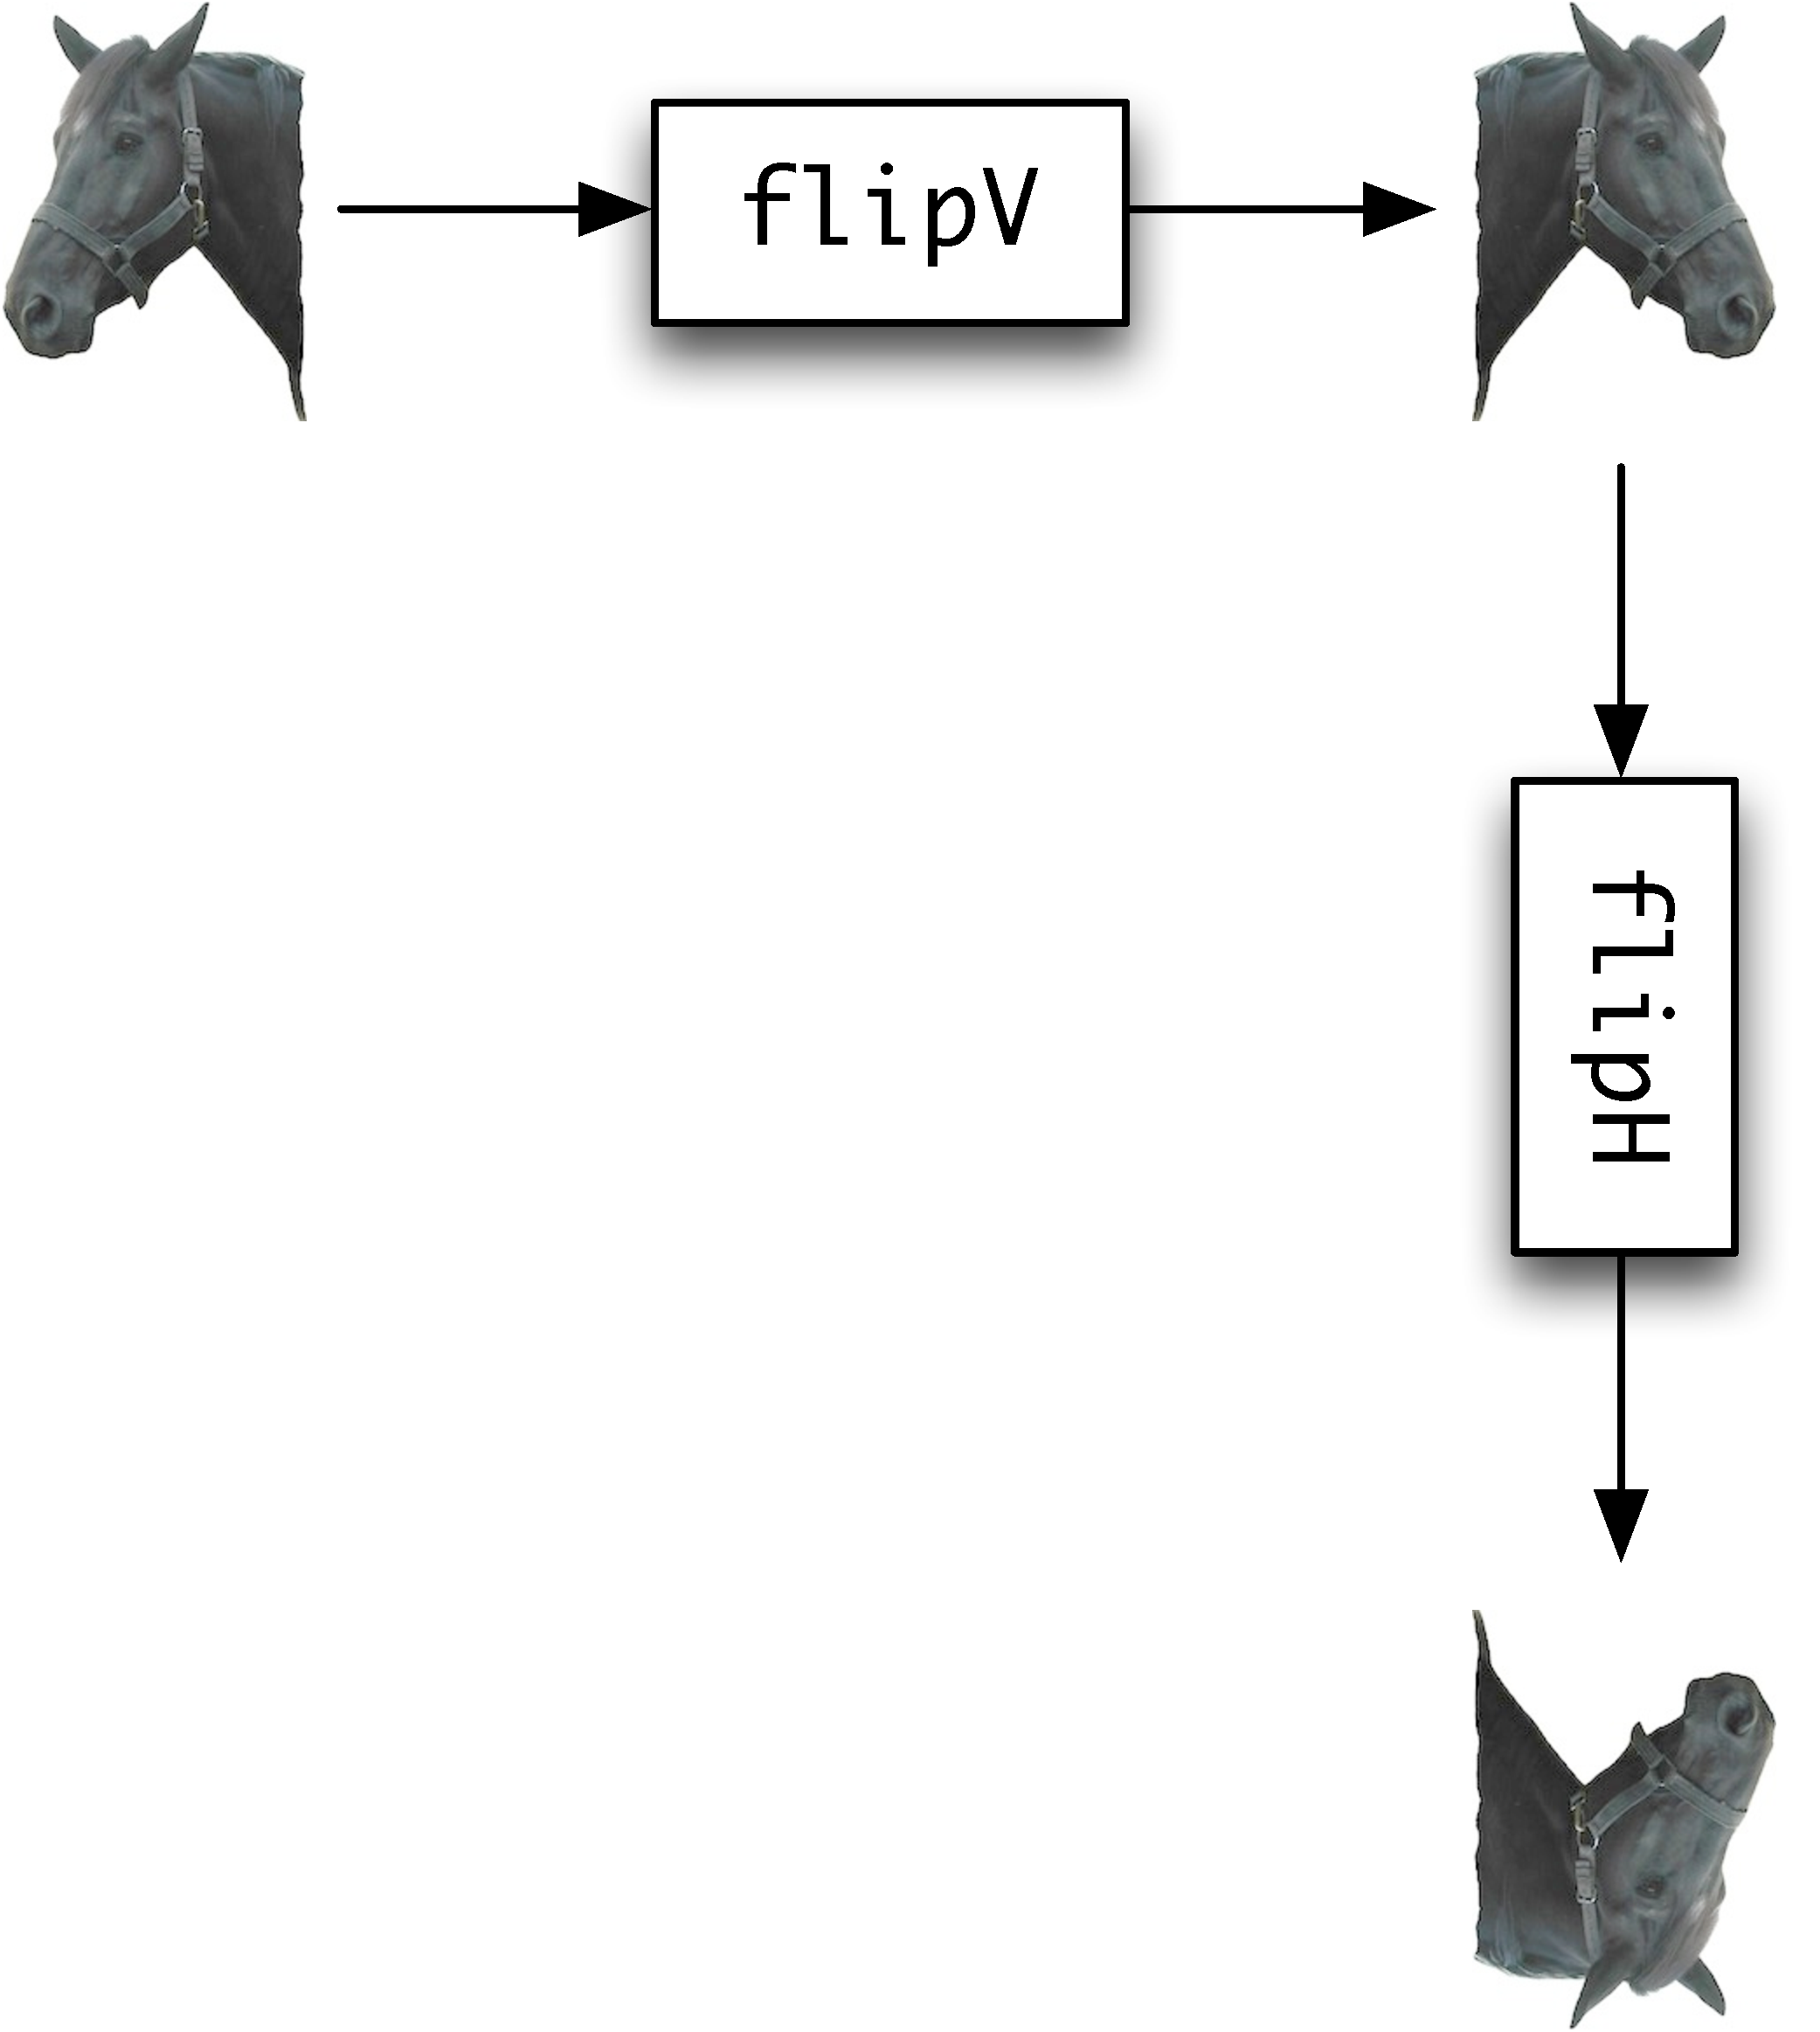
\includegraphics[width=3.0in]{Pictures/VthenH.pdf}
\end{center}
\caption{Calculating a rotation}
\label{flipping}
\end{figure}


\noindent
Another example is the definition
\begin{alltt}\minx{rotateHorse}
rotateHorse :: Picture
rotateHorse = flipH (flipV horse)
\end{alltt}
where Figure \ref{flipping} illustrates the evaluation of the right-hand side,
assuming that the function \texttt{flipH} has the effect of reflecting a
\texttt{Picture} in a horizontal mirror. The effect of these
two reflections is to rotate the picture through $180^\circ$.

In Section \ref{exprEval} we explained that GHCi works rather
like a calculator in evaluating expressions. How will it evaluate an
expression like
\begin{alltt}
size - 17
\end{alltt}
for instance?
Using the definition of \texttt{size} given earlier, we can replace the left-hand side 
-- \texttt{size} -- with 
the corresponding right-hand side -- \texttt{12+13}; this gives us the expression
\begin{alltt}
(12+13) - 17
\end{alltt}
and so by doing some arithmetic we can
see that the value of the expression is \texttt{8}.

The definitions we have seen so far are simply of constant values; we
now turn find out how functions are defined.

\section{Function definitions}
\label{funDefs}
\index{definition!function}
\index{function!definition}

We can also define functions, and we look at some simple examples now.
To square an integer we can say
\begin{alltt}
square :: Integer -> Integer\minx{square}
square n = n*n
\end{alltt}
where diagrammatically the definition is represented by
\begin{center}\minx{horse}\index{pictures!horse}
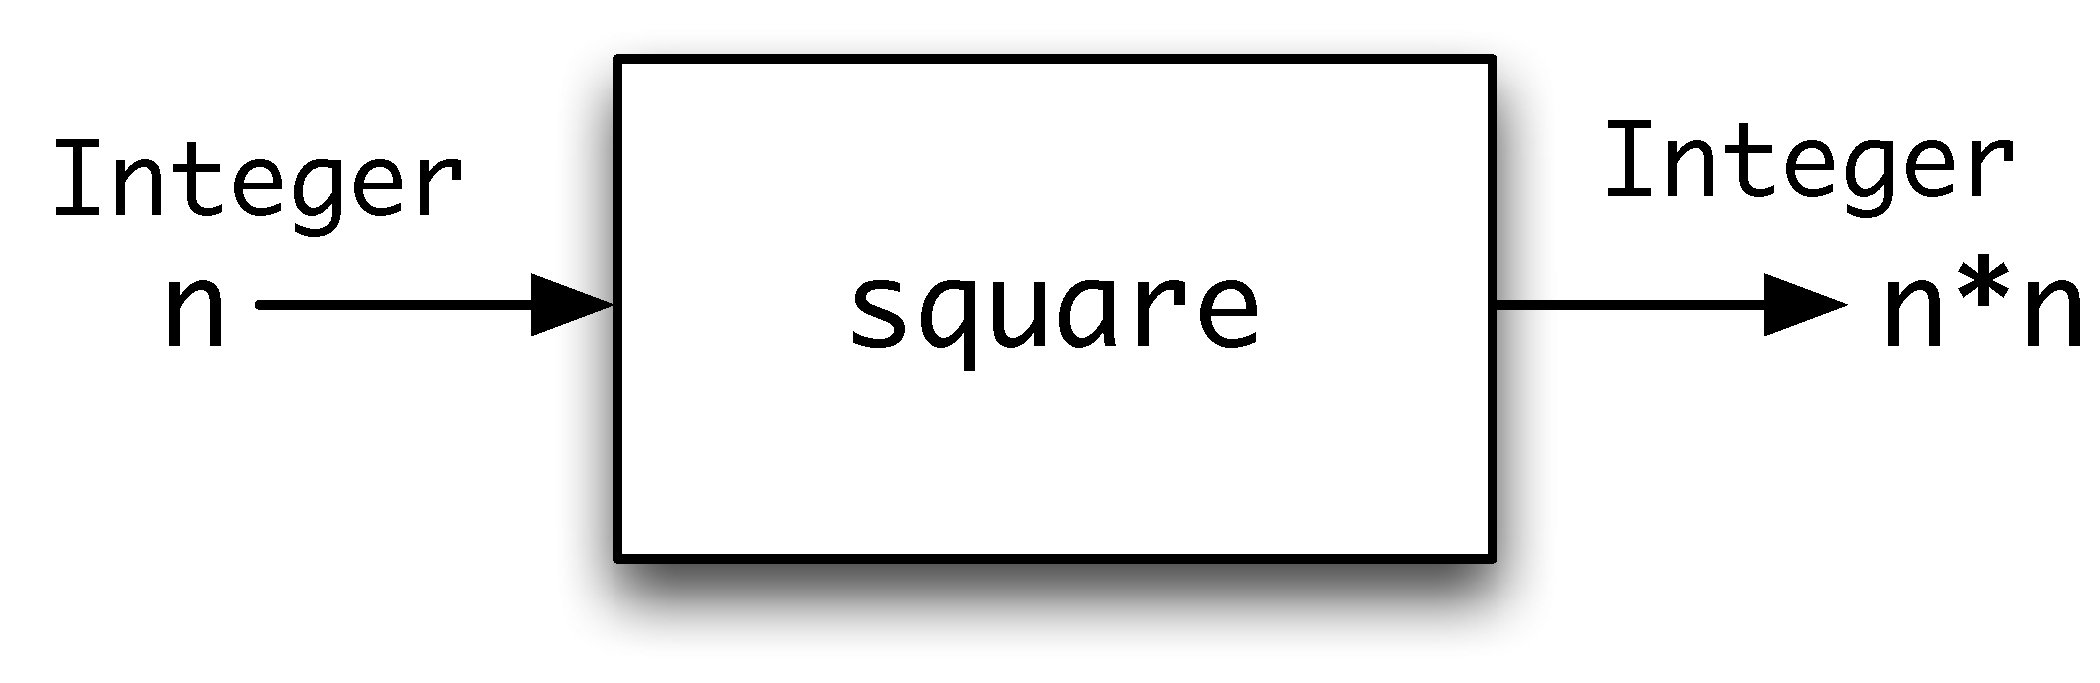
\includegraphics[width=3in]{Pictures/square.pdf}
\end{center}
The first line of the Haskell definition of \texttt{square}
declares the type of the thing being defined. The arrow \texttt{->} signifies that this is a function, with one input, an \texttt{Integer}, appearing before the arrow, and, coming after the arrow, a result of type
\texttt{Integer}. So, we can read \texttt{square ::\ Integer -> Integer} as 
\begin{quote}
``\texttt{square} is a function taking an \texttt{Integer} to an \texttt{Integer}''
\end{quote}\index{reading `\texttt{::}'}
The second line gives the definition of the function: the
equation\index{equation} says that when \texttt{square} is applied to an
\textbf{unknown}\index{unknown} or \textbf{variable}\index{variable}
\texttt{n}, then the result is \texttt{n*n}. How should we read an
equation like this? Because \texttt{n} is an arbitrary, or unknown value, it 
means that the equation holds {\em whatever the
value of\/} \texttt{n}, so that it will hold whatever integer expression we put
in the place of \texttt{n}, so that, for instance
\begin{alltt}
square 5 = 5*5
\end{alltt}
and
\begin{alltt}
square (2+4) = (2+4)*(2+4)
\end{alltt}
This is the way that the equation is used in evaluating an expression
which uses \texttt{square}. If we need to evaluate
\texttt{square} applied to the expression \texttt{e}, we replace the
application \texttt{square e} with the corresponding right-hand side,
\texttt{e*e}.

In general a simple function definition will take the form
\begin{center}\index{function definition!general case!single equation}
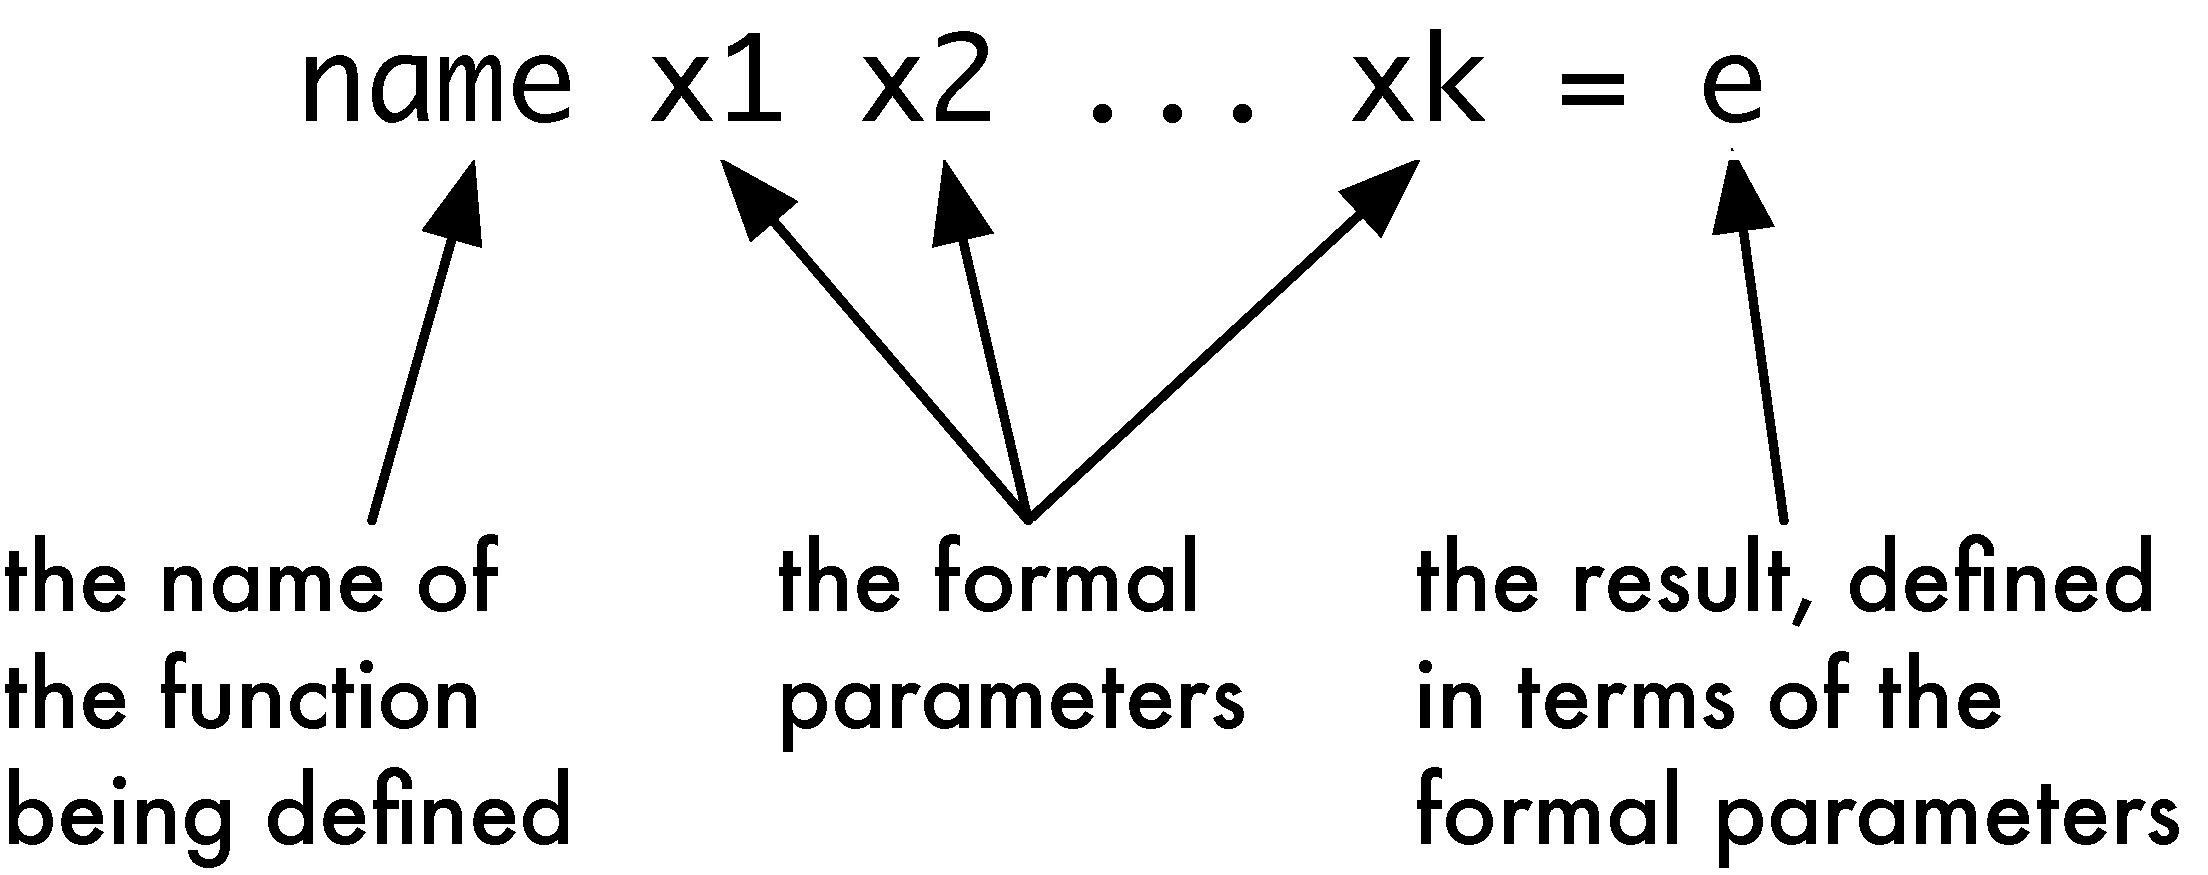
\includegraphics[width=3in]{Pictures/funDef.pdf}
\end{center}
The variables used in an equation defining a
function stand for arbitrary values: the definition holds for whatever value is chosen for these inputs. These variables are called the \textbf{formal parameters}\index{formal
parameter}\index{parameter!formal} of the function because they stand for arbitrary
values of the parameters: the \textbf{actual} parameters\index{actual
parameter}\index{parameter!actual} are supplied when the function is applied, as in \texttt{square 7}, where \texttt{7} is the actual parameter to \texttt{square}. We'll
only use `formal' and `actual' in the text when we need to draw a
distinction between the two; in most cases it will be obvious what is
meant when `parameter' is used.

Accompanying the definition of the function is a statement or \textbf{declaration}\index{type declaration} 
of its
type. That will look like this, using the \texttt{scale} function
over pictures as an example:
\begin{center}
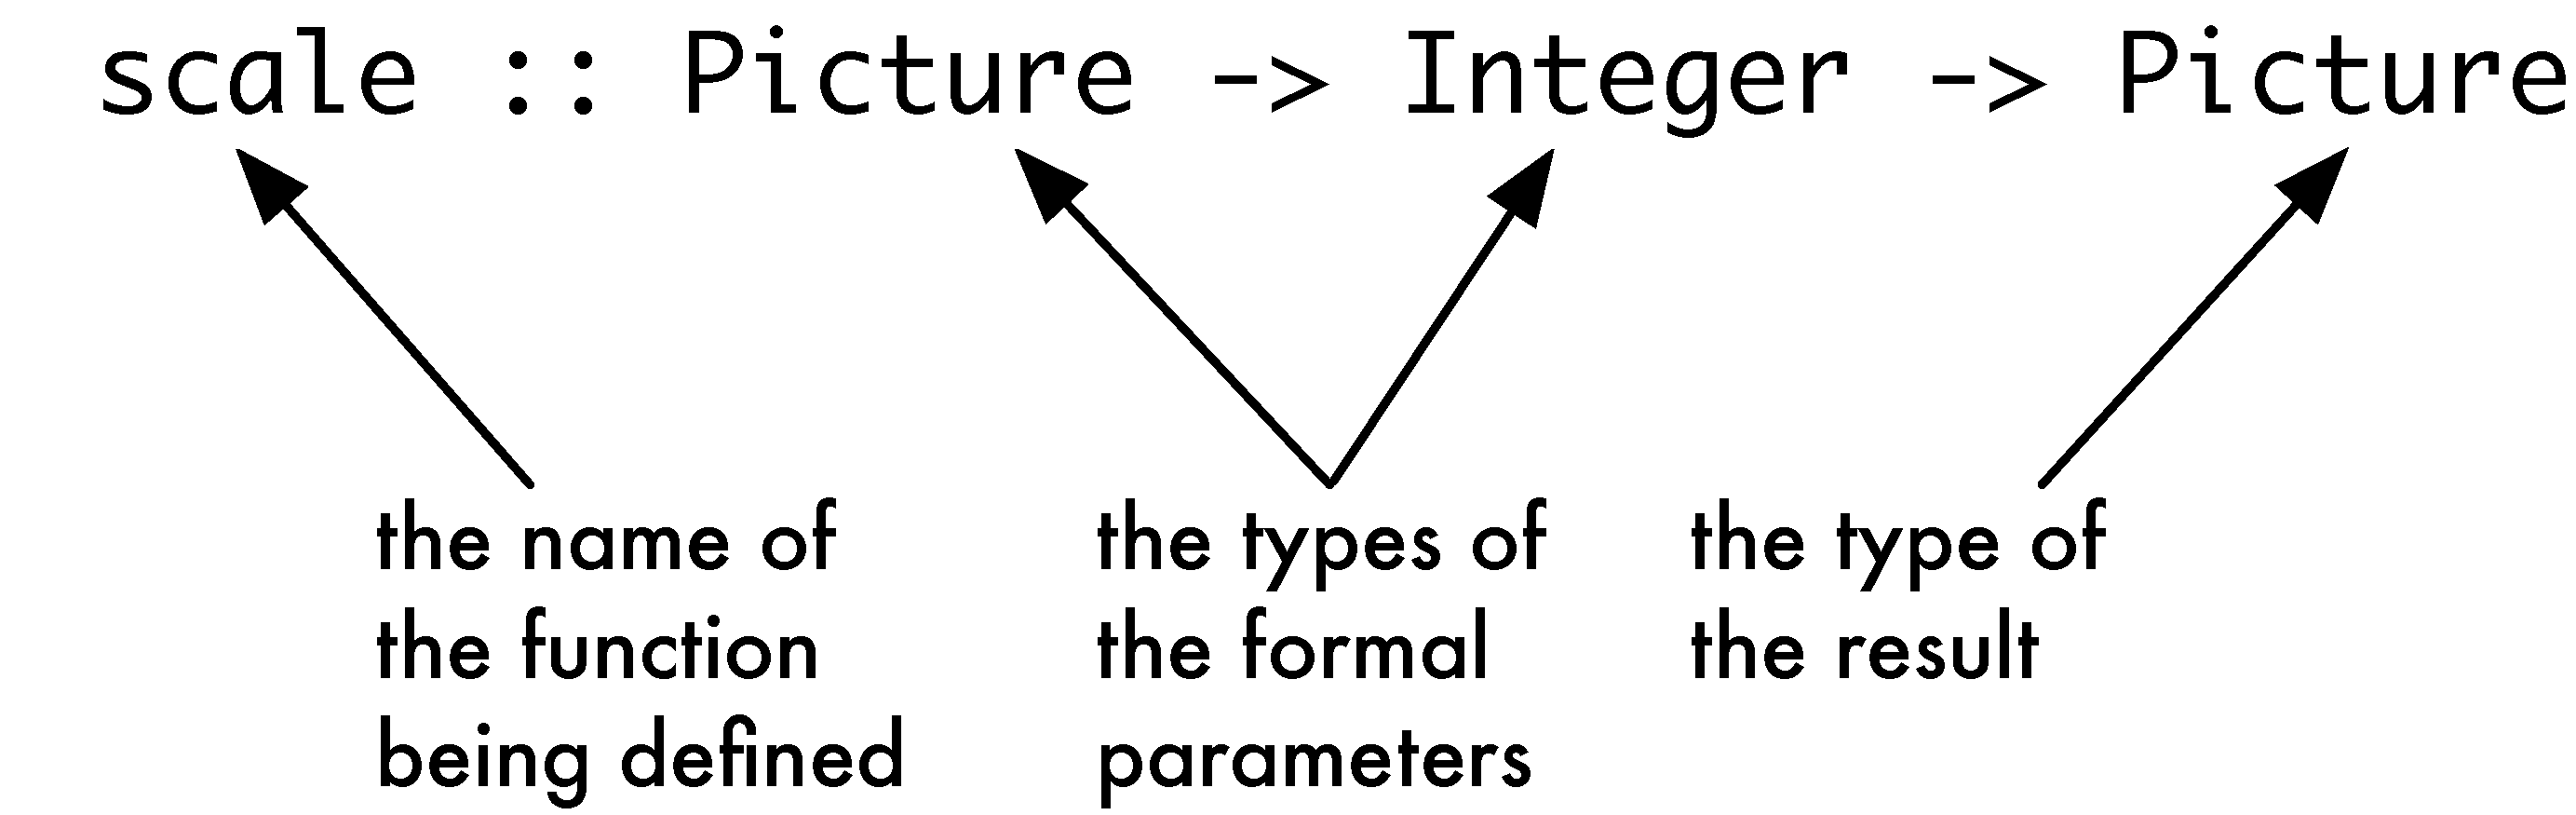
\includegraphics[width=4in]{Pictures/typeDiag.pdf}
\end{center}\index{scale@\texttt{scale}!type declaration}
In the general case we have
\begin{center}\index{type declaration!for function}
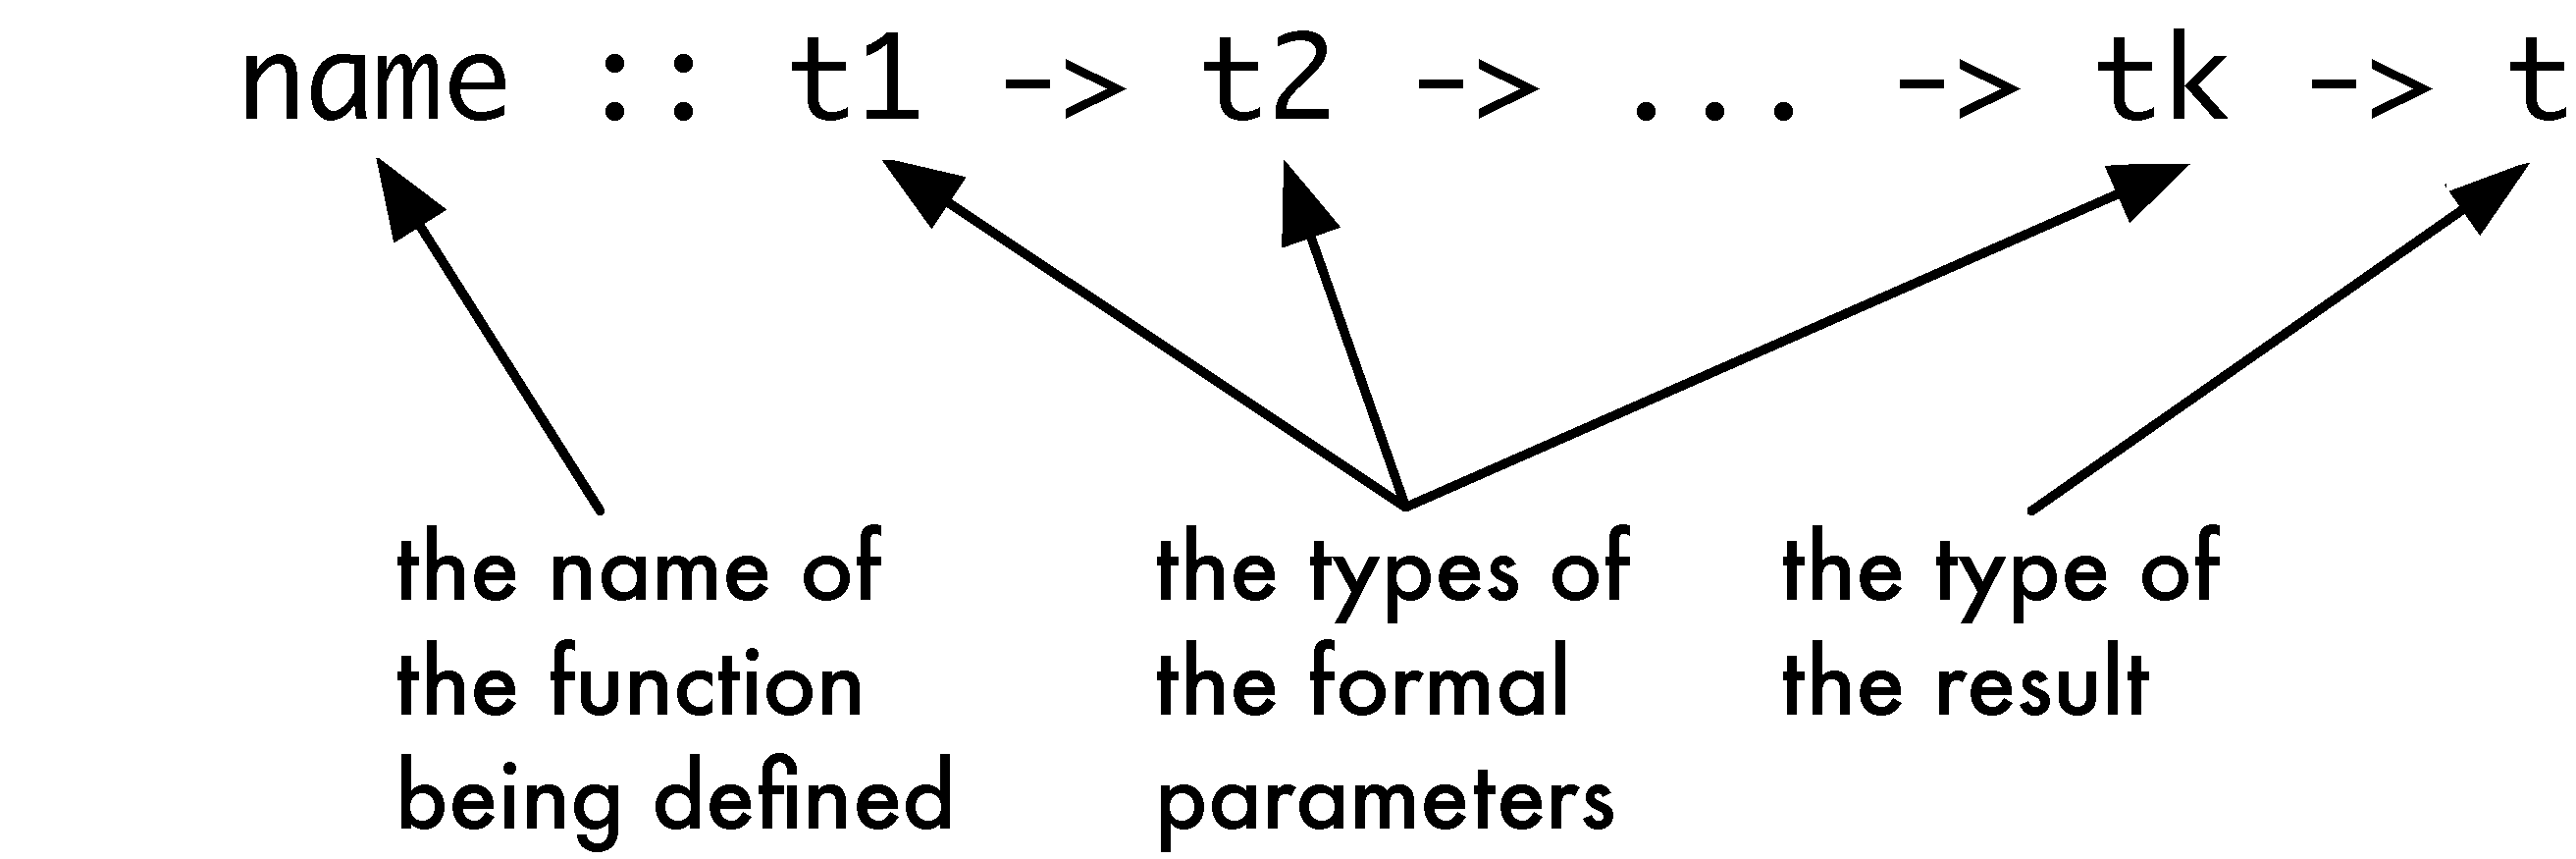
\includegraphics[width=4in]{Pictures/funTypeDef.pdf}
\end{center}
The definition of \texttt{rotateHorse} in Section \ref{defsIntro}
suggests a general definition of a rotation function. To
rotate {\em any\/} picture we can perform the two reflections, and so we
define
\begin{alltt}
rotate :: Picture -> Picture
rotate pic = flipH (flipV pic)
\end{alltt}
We can read the definition like this:
\begin{quote}
To \texttt{rotate} a picture \texttt{pic}, we first apply \texttt{flipV}
to form \texttt{(flipV pic)}; we then apply \texttt{flipH} to reflect this in a horizontal mirror, giving the result \texttt{flipH (flipV pic)}.
\end{quote}
Given this definition, we can replace the definition of
\texttt{rotateHorse} by
\begin{alltt}
rotateHorse :: Picture
rotateHorse = rotate horse
\end{alltt}
which states that \texttt{rotateHorse} is the result of applying the
function \texttt{rotate} to the picture \texttt{horse}.

The pattern of definition of \texttt{rotate} -- `apply one function, and
then apply another to the result' -- is so common that Haskell gives a
way of combining 
functions directly in this way. We define
\begin{alltt}\minx{rotate}
rotate :: Picture -> Picture
rotate = flipH . flipV
\end{alltt}\label{here}
The `\texttt{.}'\minx{.} in the definition signifies \textbf{function
composition}\index{function composition}\index{composition|see{function composition}}, in which
the output of one function becomes the input of another. In pictures, 
\begin{center}
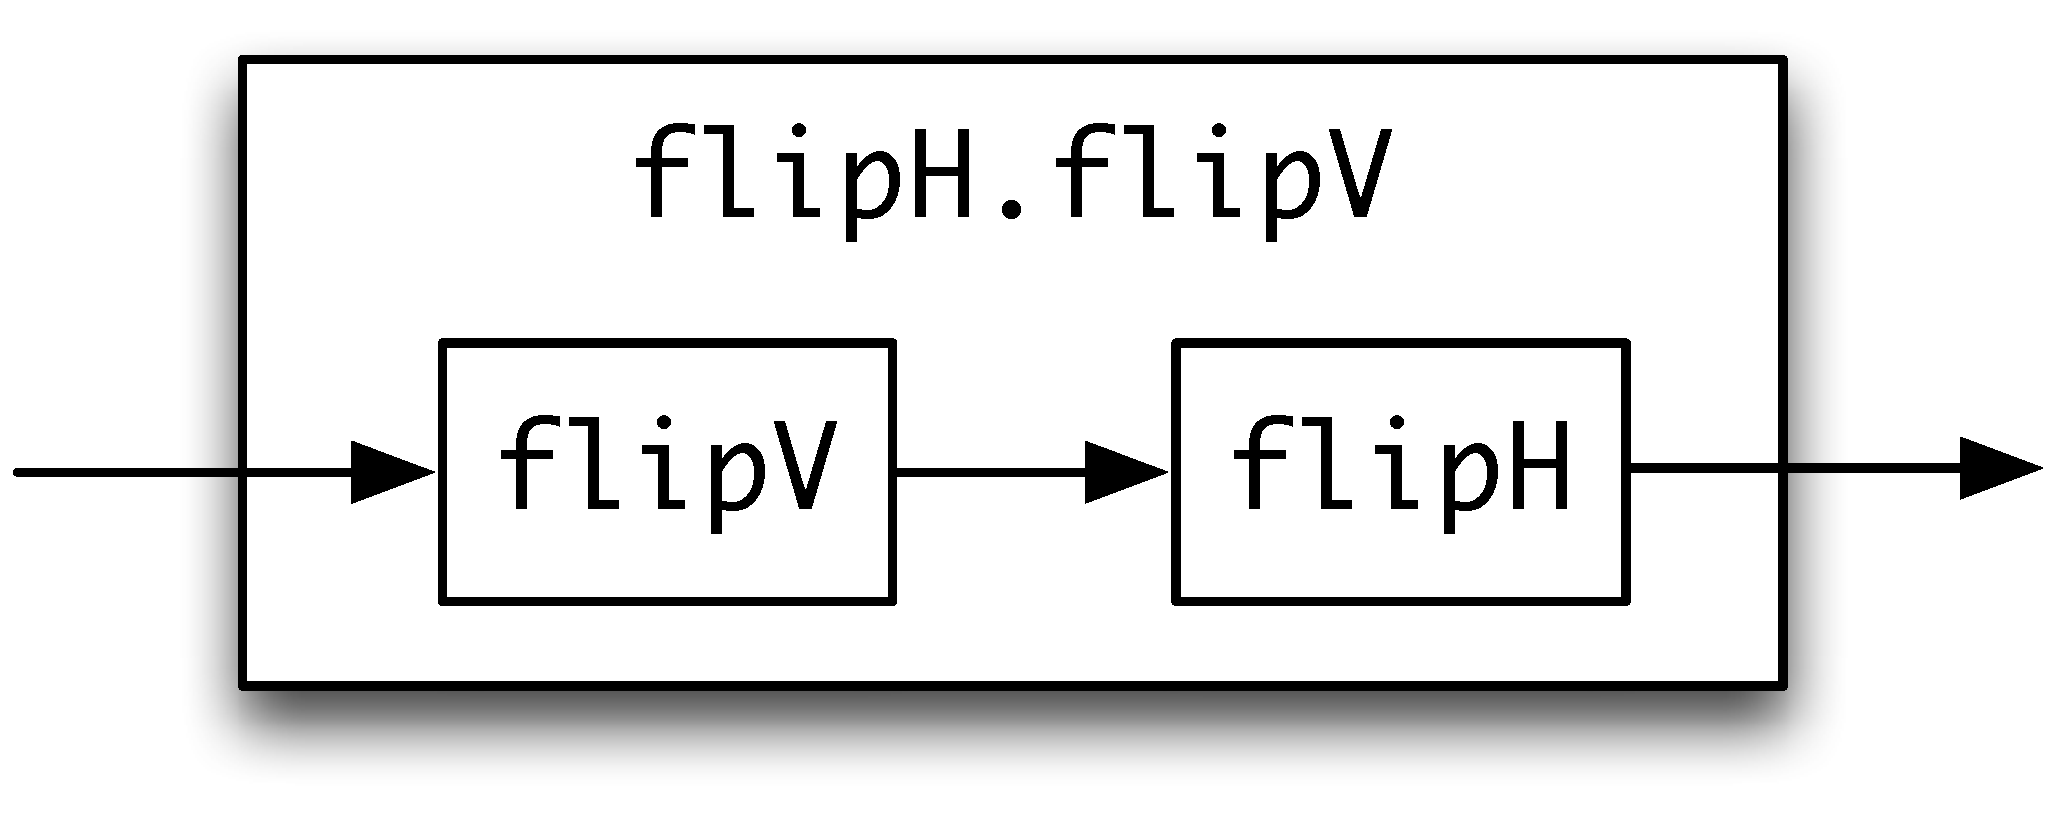
\includegraphics[width=3in]{Pictures/HVcompos.pdf}
\end{center}
we see the creation of a new function by connecting together the input
and output of two given functions: obviously this suggests many other
ways of connecting together functions, many of which we will look at in
the chapters to come.

The direct combination of functions is one example of the
power of functional programming: we are able to combine functions using
an operator like `\texttt{.}' just as we can combine
numbers using `\texttt{+}'. We use the term `\textbf{operator}'\index{operator} here
rather than `function' since `\texttt{.}' is written between its
arguments rather than before them; we discuss operators in more detail
in Section \ref{syntax}.

The direct combination of functions by means of the operator `\texttt{.}'
which we have seen here 
is not possible in other programming
paradigms, or at least it would be an `advanced' aspect of the language,
rather than appearing on page \pageref{here} of an
introductory text.



\section{Types and functional programming}
\label{typesFP}
\index{type!importance of types}

What is the role of types in functional programming? Giving a type to a
function first of all gives us crucial information about how it is to be
used. If we know that
\begin{alltt}
scale :: Picture -> Integer -> Picture
\end{alltt}\index{scale@\texttt{scale}!type declaration}\index{type declaration!understanding}
we know two things immediately.
\begin{itemize}
\item First, \texttt{scale} has two arguments: the first is a
\texttt{Picture} and the second an \texttt{Integer}; this means that
\texttt{scale} can be applied to \texttt{horse} and \texttt{3}.
\item The result of applying \texttt{scale} to this \texttt{Picture} and \texttt{Integer}
will be a \texttt{Picture}.
\end{itemize}
The type thus does two things. First, it expresses a
\textbf{constraint}\index{constraint}\index{type!constraint} on how the
function \texttt{scale} is applied: it must be applied 
to a \texttt{Picture} and an \texttt{Integer}. Second, the type tells us
what the result is if the function is correctly applied: in this case
the result is a \texttt{Picture}.

Giving types to functions and other things not only tells us how they
can be used; it is also possible to check automatically that functions
are being used in the right way and this process -- which is called
\textbf{type checking}\index{type checking} -- takes place in Haskell. If we
use an expression like 
\begin{alltt}
scale horse horse
\end{alltt}
we will be told that we have made an error in applying \texttt{scale} to
two pictures
when a picture and a number are what was expected. Moreover, this can be done without knowing
the {\em values\/} of \texttt{scale} or \texttt{horse} -- all that we need to know 
to perform the check is the {\em types\/} of the things concerned.
Thus, \textbf{type errors}\index{type error} like these 
are caught before programs are used or expressions
are evaluated.

It is remarkable how
many errors, due either to mistyping or to misunderstanding the problem, are made
by novices and experienced programmers alike.  The Haskell type system
therefore helps us to write correct programs, and to avoid a large proportion 
of programming pitfalls, both 
obvious and subtle, typos and misunderstandings. This is something which you particularly appreciate if you do use other languages without this kind of type checking, where you need to trace back from a particular error that happens during evaluation to its source.

\subsection*{Type abstraction}
\index{abstraction!type}\index{type!abstract}

Before moving on, there is another important point which we'll
explore later in the book. In Sections \ref{defsIntro} and \ref{funDefs}
we gave definitions of
\begin{alltt}\minx{Picture}\minx{rotate}
blackHorse :: Picture
rotate     :: Picture -> Picture
\end{alltt}
which \textbf{use} the type \texttt{Picture} and some functions already defined
over it: \texttt{flipH} and \texttt{flipV}. We were able to
write the definitions of
\texttt{blackHorse} and \texttt{rotate} {\em without
knowing anything about\/} how the type of \texttt{Picture}s or the functions working with \texttt{Picture}s were actually defined. We can use these functions because we know their types, so we know what they have to be applied to, and what type their results will be.

Treating the type \texttt{Picture} in this way is called
\textbf{type abstraction}:
as users of the type we don't need to concern ourselves with how the type is
defined. The advantage of this is that the definitions we give apply {\em
however\/} pictures are modelled. We might choose to model them in
different ways in different situations; whatever the case, the function
composition
\texttt{flipH .\ flipV} will rotate a
picture through $180^\circ$. We'll see this in practice in Section \ref{two-models} where we give two, very different, models of pictures; 
Chapter \ref{adt} discusses this in more
detail, and explains the Haskell mechanism to support type abstraction.



\section{Calculation and evaluation}
\index{calculation}\index{evaluation}

We have explained that GHCi can be seen as a general calculator, using
the functions and other things defined in a functional program. When we
evaluate an expression like
\begin{alltt}
23 - (double (3+1))\hfill(\ddag)
\end{alltt} 
we need to use the definition of the function:
\begin{alltt}
double :: Integer -> Integer
double n = 2*n\hfill(dbl)
\end{alltt}\minx{double}
This we do by replacing the unknown \texttt{n} in the definition
\texttt{(dbl)} by the
expression \texttt{(3+1)}, giving 
\begin{alltt}
double (3+1) = 2*(3+1)
\end{alltt}
Now we can replace \texttt{double (3+1)} by \texttt{2*(3+1)} in \texttt{(\ddag)}, and
evaluation can continue.

One of the distinctive aspects of functional programming is that such a
simple 
`calculator' model is a complete description of computation in Haskell. Because the model is so straightforward, we can perform
evaluations in a \textbf{step-by-step}\index{evaluation!step-by-step}
manner; in this text we call these step-by-step evaluations
\textbf{calculations}\index{calculation}.
As an example, we now show the calculation of the expression with which we 
began the discussion.
\begin{alltt}
23 - (double (3+1))
\step 23 - (2*(3+1))\hfill\textrm{using} \texttt{(dbl)}
\step 23 - (2*4) \hfill\textrm{arithmetic}
\step 23 - 8 \hfill\textrm{arithmetic}
\step 15 \hfill\textrm{arithmetic}
\end{alltt}
where we have used `\step'\index{\step} to indicate a step of the calculation, and on
each line we indicate at the right-hand margin how we have reached that
line. For instance, the second line of the calculation:
\begin{alltt}
\step 23 - (2*(3+1))\hfill\textrm{using} \texttt{(dbl)}
\end{alltt}
says that we have reached here using the definition of the
\texttt{double} function, \texttt{(dbl)}.

In writing a calculation it is sometimes useful to \underline{underline}\index{underlining@\underline{underlining}}
the part of the expression which gets modified in transition to the next
line. This is, as it were, where we need to focus our attention in
reading the calculation. The calculation above will have underlining
added like this:
\begin{alltt}
23 - \underline{(double (3+1))}
\step 23 - (2*\underline{(3+1)})\hfill\textrm{using} \texttt{(dbl)}
\step 23 - \underline{(2*4)} \hfill\textrm{arithmetic}
\step \underline{23 - 8} \hfill\textrm{arithmetic}
\step 15 \hfill\textrm{arithmetic}
\end{alltt}
In what is to come, when we introduce a new feature of Haskell we shall
show how it fits into this line-by-line model of evaluation. This has
the advantage that we can then explore new ideas by writing down
calculations which involve these ideas.


\section{The essence of Haskell programming}
\index{programming paradigms!comparison}

We've learned enough about functional programming in Haskell to compare it with other kinds of programming paradigm, particularly OO and other imperative languages. First we'll summarise the essentials of Haskell, and then look at how it differs from others approaches.

So, what makes functional programming in Haskell special? Working in Haskell we concentrate on using a rich collection of data types -- including functions themselves, as well as types defined by the user -- to model the objects in the problem domain. Programming over these is done by writing functions: functions are defined by equations like
\begin{alltt}
rotate :: Picture -> Picture
rotate pic = flipH (flipV pic)\hfill\texttt{(rotate)}
\end{alltt}
Finally, computing with these functions is done by calculation, or evaluation, using the definitions to calculate a result as we saw in the last section. In a equation like \texttt{(rotate)}, \texttt{pic} is a variable, in the mathematical sense of something that stands for an \emph{arbitrary} \texttt{Picture}.

If you know Java, or another OO or imperative language like C, C++ or C\#, then you need to understand that Haskell variables are very different from variables in these languages. A Java variable is like a box, where values can be stored: the value is changed by making an assignment. In Java we compute by changing these contents, or the\texttt{state} as it is called. Methods which change state are said to have \textbf{side-effects}\index{side-effect}. 

By contrast, Haskell variables don't vary, and the way we program is to write functions which describe how particular data values are related. These functions don't have side-effects, and there is no state in Haskell. We'll find about how all of this works in the chapters to come, we can summarize the important advantages now.
\begin{itemize}
\item
Haskell programs are \emph{higher-level}: they can be read as a direct description of \emph{what} are the relationships between input and output data, rather than covering the details of \emph{how} a result is computed in a series of steps that change the values of variables.
\item
Functions in Haskell can themselves be passed around just like any other \emph{data}. So, we can use functions as well as all the other Haskell types when we're modelling complex problems.
\item
Haskell functions are without side-effects, but in Haskell it's possible to do I/O, work with files, and inter-operate with other programming languages. We can do this using \emph{monads} which allow these `computational effects' to be embedded inside Haskell and its type system.
\item
Haskell programs are easy to \emph{parallelise}, and to run efficiently on multicore hardware, because there is no state to be shared between different threads. In Java different treads share the same state, and it's very hard to make sure that a Java program will run efficiently -- or even correctly -- in a multicore environment.
\item
If definitions are equations, then it's possible to think of them as expressing \emph{properties} of programs, and we can use these to write \emph{proofs} of other properties our programs have, and so validate what they do.
\item
There are often many different ways of solving the same problem, and when we begin to try to solve a problem it can be very hard to know which approach to take. Because Haskell programs are free of side-effects it's much easier to transform or \emph{refactor} our programs to have a different design, as we might need to do before extending or modifying our program.
\end{itemize} 
Taking these together, we can see why Haskell is popular for many tasks, and particularly for writing domain-specific languages, which we look at now.


\section{Domain-specific languages}
\index{domain-specific language|see{DSL}}\index{DSL|(} 

Haskell is a general-purpose programming language: it can be used to solve any kind of programming problem. Other languages, called \textbf{domain-specific languages} (\textbf{DSLs}) or \textbf{little languages}, are designed to solve problems in a particular domain. For example, this book has been written using \LaTeX, a language for typesetting; other DSls are used for hardware design (Verilog), statistics (R, Excel) and graph layout (GraphViz).
Stand-alone DSLs like these have the advantage that everything about them, from the way that programs are written to the details of what they mean, can be adapted to the particular domain. On the other hand, all the infrastructure has to be built from scratch.

A different approach is not to build the DSL from scratch, but instead to embed it in an existing programming language. These \textbf{embedded domain-specific languages}\index{DSL!embedded} can take advantage of everything that the programming language provides, while expressing the concepts of the particular domain as well. Haskell has been particularly successful as a basis for embedding DSLs, including Lava \cite{lava} for circuit simulation and layout, Paradise \cite{paradise} for pricing financial products and Orc \cite{orc} for orchestrating scientific computations.

Why has Haskell been particularly successful for embedding DSLs? The rich set of data types -- including functions and user-defined \texttt{data} types -- which can be used to model the underlying domains; the absence of side-effects makes it possible to write models which focus on the data, independent of any state. More advanced aspects of Haskell also help the DSL writer. Some are beyond the scope of this text, but we'll cover three important features. Polymorphism and type classes are two different mechanisms to make it possible for functions to be used over multiple types: this allows a DSL to be interpreted in different ways; for example, this allows a hardware DSL can be used both for simulation and layout of circuits. Monads allow DSLs to have side-effects in a controlled way. We'll come back to this discussion as we look at DSLs in Haskell in Chapter \ref{dsls}.
\index{DSL|)} 


\begin{figure}[t]
\begin{center}
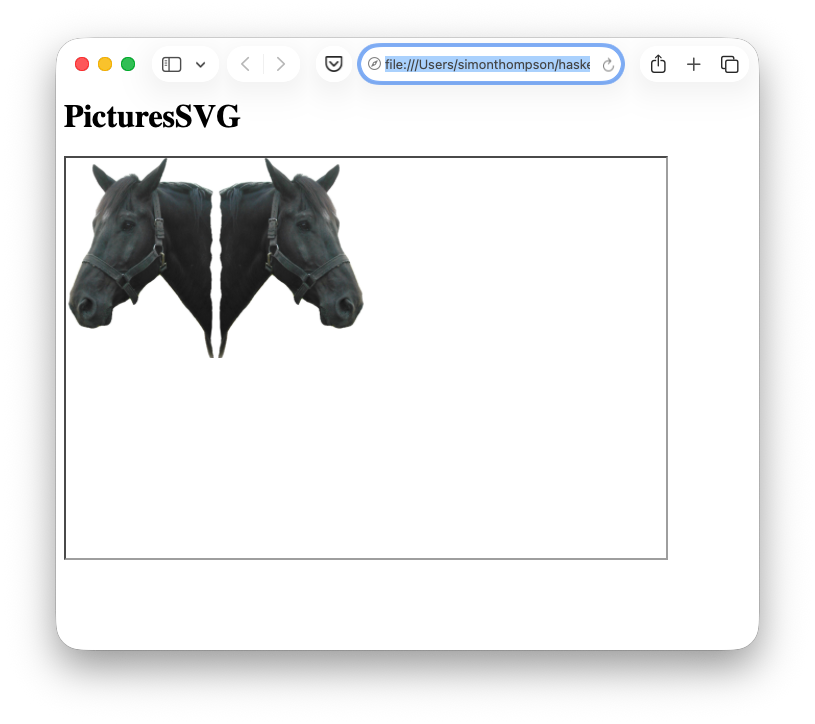
\includegraphics[width=\textwidth]{Pictures/ScreenSVG.png}
\end{center}
\caption{Viewing \texttt{Pictures} in a web browser}
\label{svgpix}
\end{figure}



\section{Two models of \texttt{Picture}s}
\label{two-models}
\index{pictures|(}\index{DSL!pictures}


This section looks at the pictures example as a small DSL, and gives two models -- or implementations -- of the pictures DSL.

\subsection*{The \texttt{Picture} DSL}

We can describe the DSL for \texttt{Picture}s by giving the type declarations of its constructs.
\begin{alltt}
horse        :: Picture

flipH        :: Picture -> Picture
flipV        :: Picture -> Picture
invertColour :: Picture -> Picture

above        :: Picture -> Picture -> Picture
beside       :: Picture -> Picture -> Picture

scale        :: Picture -> Integer -> Picture
\end{alltt}
We form complex pictures by combining these into expressions, such as
\begin{alltt}
horse `above` (flipH horse)
\end{alltt}
but because the DSL is embedded in Haskell we can use all the facilities of Haskell too.  We might make a complicated calculation of how much we want to scale a picture,
\begin{alltt}
scale (horse `above` (flipH horse)) (complicated Integer calculation)
\end{alltt}
but we can also use the facilities of Haskell for naming \texttt{Picture}s 
\begin{alltt}
bigPic = scale (horse `above` (flipH horse)) 42
\end{alltt}
and defining other functions
\begin{alltt}
mirror pic = pic `beside` (flipV pic)
\end{alltt}


\begin{figure}[t]
\begin{center}
\begin{alltt} 
.......##...               ......##....               ...##.......
.....##..#..               .....#.#....               ..#..##.....
...##.....#.               ....#..#....               .#.....##...
..#.......#.               ...#...#....               .#.......#..
..#...#...#.               ..#...#.....               .#...#...#..
..#...###.#.               .#....#..##.               .#.###...#..
.#....#..##.               ..#...###.#.               .##..#....#.
..#...#.....               ..#...#...#.               .....#...#..
...#...#....               ..#.......#.               ....#...#...
....#..#....               ...##.....#.               ....#..#....
.....#.#....               .....##..#..               ....#.#.....
......##....               .......##...               ....##......

horse                      flipH horse                flipV horse
\end{alltt}
\end{center}
\caption{ASCII-art pictures}
\label{Horses}\minx{horse}
\end{figure}


\subsection*{SVG pictures}

The pictures we've seen so far in this chapter are from a model of pictures which can be displayed in web browsers supporting the SVG standard\cite{SVG},\index{SVG} as shown in Figure \ref{svgpix}. The web page allows you to view pictures ``rendered from'' Haskell descriptions; we'll come back to the details of how this is done in Section \ref{ShowBrowser}, page \pageref{ShowBrowser}. For now the message is that you can use the DSL just knowing the types of the functions, as they tell you all you need to know to use them: for each function they tell us the types of the inputs they should be applied to and the type of the result.

\subsection*{Pictures and lists}


We include this section in the first chapter of the book for two reasons.
To start with, we want to describe a second way in which \texttt{Picture}s can be 
modelled in Haskell. 
Secondly, we want to provide an
informal preview of a number of aspects of Haskell which make it
a powerful and distinctive
programming tool. As we go along we will indicate
the parts of the book where we expand on
the topics first introduced here.

Our model consists of two-dimensional, monochrome pictures built 
from \textbf{characters}\index{characters}.
Characters are the individual letters,
digits, spaces and so forth which can be typed at the computer keyboard and which 
can also be shown on a computer screen. In Haskell the characters are
given by the built-in type
\texttt{Char}\minx{Char}. 
This model has the advantage that it is straightforward to view these
pictures on a computer terminal window. 


Our version of the \texttt{horse} picture, and the same picture
flipped in horizontal and vertical mirrors are shown in Figure \ref{Horses},
where we use dots to show the white parts of the pictures.

How are the pictures built from characters? In our model we think of
a picture as being made up of
a \textbf{list}\index{lists} of lines, that is a collection of
lines coming one after another in order. Each line can be seen in a similar way
as a list of characters. Because we often deal with collections of things when programming, 
lists are built into Haskell. More specifically, given any type -- like characters or lines
-- Haskell contains a type of lists of that type, and so in particular we can model pictures
as we have already explained, using lists of characters
to represent lines, and lists of lines to represent pictures.

With this model of \texttt{Picture}s, we can begin to think about how to
model functions over pictures. A first definition comes easily; to
reflect a picture in a horizontal mirror each line is unchanged, but
the order of the lines is reversed: in other words we reverse the list
of lines:
\begin{alltt}
flipH = reverse\minx{flipH}\minx{reverse}
\end{alltt}
where \texttt{reverse} is a built-in function to reverse the order of items
in a list.
How do we reflect a picture in a vertical mirror? The ordering of the
lines is not affected, but instead {\em each line is to be reversed}. We can write
\begin{alltt}
flipV = map reverse\minx{flipV}
\end{alltt}
since \texttt{map}\index{map@\texttt{map}} is the Haskell function which applies a function
to each of the items in a list, individually.
In the definitions of \texttt{flipH} and \texttt{flipV} we can begin to see the power 
and elegance of
functional programming in Haskell.
\begin{itemize}
\item 
We have used \texttt{reverse} to reverse a list of lines in
\texttt{flipH} and to reverse each line in \texttt{flipV}: this is
because the same
definition of the function \texttt{reverse} can be used over {\em every\/}
type of list. This is an example of polymorphism,\index{polymorphism} or generic
programming, which is examined in detail in Section \ref{poly}.
\item 
In defining \texttt{flipV} we see the function \texttt{map}
applied to its argument \texttt{reverse}, {\em which is itself a
function}. This makes \texttt{map} a very general function, as it can have
any desired action on the elements of the list, specified by the function
which is its argument. This is the topic of Chapter \ref{patternsGen}.
\item 
Finally, the {\em result\/} of applying \texttt{map} to
\texttt{reverse} is itself a function. This covered in Chapter \ref{gen2}.
\end{itemize}
The last two facts show that functions are `first-class citizens'
\index{first-class citizens, functions} 
\index{function!first-class citizens}
and
can be handled in exactly the same way as any other sort of object like
numbers or pictures. The combination of this with polymorphism means
that in a functional language we can write very general functions like
\texttt{reverse} and \texttt{map}, which can be applied in a multitude of
different situations.

The examples we have looked at here are not out of the ordinary. We can see that
other functions over pictures have similarly simple definitions. We
place one picture \texttt{above} another simply by joining together the two 
lists of lines to make one list. This is done by the built-in operator
\texttt{++}\minx{++},
which joins together two lists:\footnote{The operator \texttt{++} is
surrounded by parentheses \texttt{(...)} in this definition so that it
is interpreted as a function; we say more about this in 
Section \ref{syntax}\index{operator!as function}.}
\begin{alltt}
above = (++)\minx{above}
\end{alltt}

To place two pictures \texttt{beside} each other we have to join corresponding
lines together, thus
\begin{alltt}\label{beside}\minx{beside}
.......##...   ++   ......##....
.....##..#..   ++   .....#.#....
...##.....#.   ++   ....#..#.... 
..#.......#.   ++   ...#...#.... 
..#...#...#.   ++   ..#...#.....
..#...###.#.   ++   .#....#..##.    
.#....#..##.   ++   ..#...###.#.    
..#...#.....   ++   ..#...#...#.     
...#...#....   ++   ..#.......#.     
....#..#....   ++   ...##.....#.      
.....#.#....   ++   .....##..#..      
......##....   ++   .......##...         
\end{alltt}
and this is defined using the function \texttt{zipWith}. This function is
defined to `zip together' corresponding elements of two lists
using -- in this case -- the operator \texttt{++}.
\begin{alltt}\index{zipWith@\texttt{zipWith}}
beside = zipWith (++) 
\end{alltt}
We shall return to these examples in Chapter \ref{gen2}.
\index{pictures|)}


\section{Tests, properties and proofs}
\label{proof}\label{pictureProps}



\noindent
How can we be sure that a program we have written does what it should? The traditional answer is to test the program on a selection of inputs, and of course we can -- and should -- do this for Haskell programs. We've got two other more powerful options, \textbf{property-based testing}\index{property-based testing}\index{testing!property-based} and \textbf{proof}, and we'll introduce those in this section, and follow them up in the rest of the book. 

\subsection*{Tests and properties}

Let's look at the example of \texttt{Picture}s from the last section: how do we test this? One way of doing this is to write tests of the form:
\begin{quote}
``apply this function to this input \ldots the output should be this''
\end{quote}
Given the picture library, we can also look at how the functions work together, and a  simple way of doing this is to check how a combination of applications works. For example, 
\begin{itemize}
\item
if we flip a picture twice in a mirror we should get back the original picture;
\item
if we flip a picture in both a horizontal and vertical mirror, it shouldn't matter the order in which we do this, as illustrated in Figure \ref{vh-hv}, page \pageref{vh-hv}.  
\end{itemize}
\begin{figure}[t]
\begin{center}
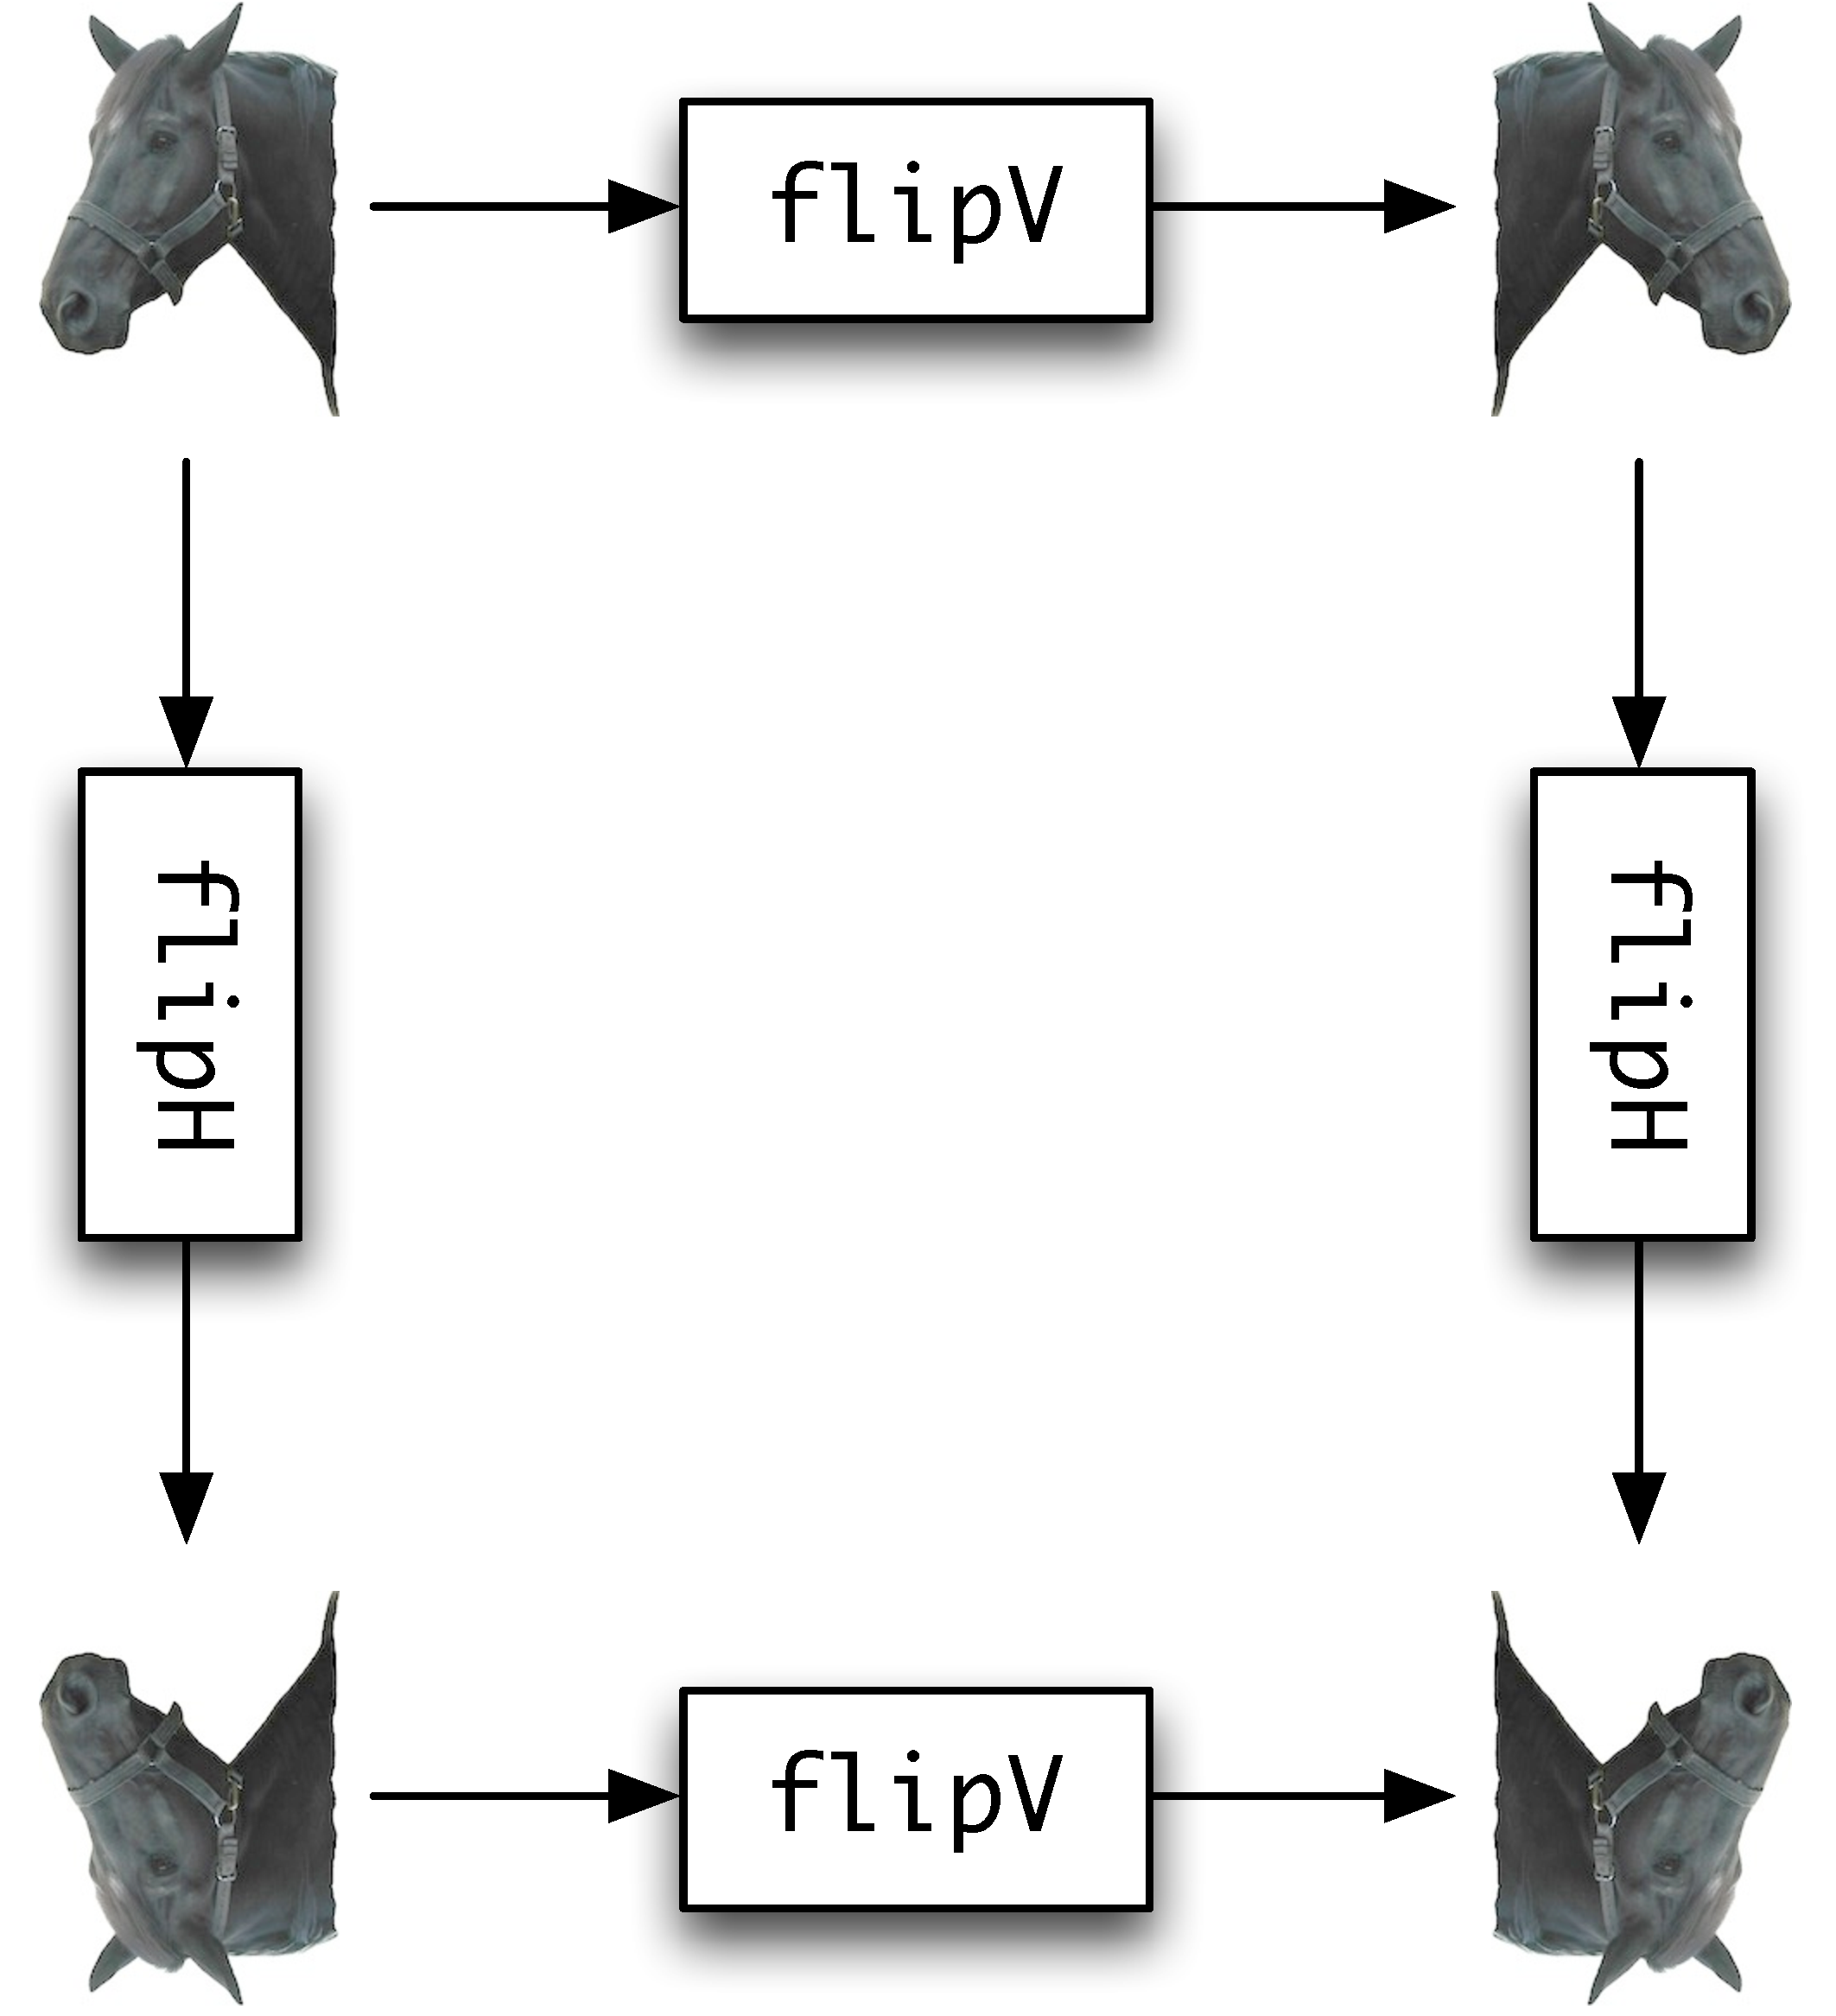
\includegraphics[width=3in]{Pictures/vh-hv.pdf}
\end{center}
\caption{Reflection in vertical and horizontal mirrors}
\label{vh-hv}
\end{figure}
These tests can be defined in Haskell, where the equality operator `\texttt{==}' is used to check whether two values are equal, returning the result \texttt{True} or \texttt{False}. These two values are the two elements of the Boolean type, \texttt{Bool}, which we come back to in the next chapter. Here are the tests:
\begin{alltt}
test_rotate, test_flipV, test_flipH :: Bool
 
test_rotate  =  flipV (flipH horse) == flipH (flipV horse)
test_flipV   =  flipV (flipV horse) == horse
test_flipH   =  flipH (flipV horse) == horse
\end{alltt}\minx{test\_rotate}
The first two tests pass, and give the answer \texttt{True}. The third fails, because we made a mistake in writing \texttt{flipV} when we should have written \texttt{flipH}; if we correct the test, it will pass as well. 


These tests work for a single input, and though \texttt{horse} is as good as any example, we ought to think of making more tests than this. \textbf{Property-based testing} in QuickCheck \cite{quickCheck}\index{QuickCheck} allows us to check whether a property holds for a whole collection of randomly generated inputs. 

What do we mean by a property?\index{property} Informally, it's something like the explanation we gave earlier ``if we flip \emph{a picture} twice in a mirror we expect to get back \emph{the original picture}'' where the ``\emph{picture}'' could be any picture. We can formalise these as Haskell functions:
\begin{alltt}
prop_rotate, prop_flipV, prop_flipH :: Picture -> Bool

prop_rotate pic  =  flipV (flipH pic) == flipH (flipV pic)
prop_flipV pic   =  flipV (flipV pic) == pic
prop_flipH pic   =  flipH (flipV pic) == pic
\end{alltt}\minx{prop\_rotate}

\begin{figure}[t]
\begin{center}
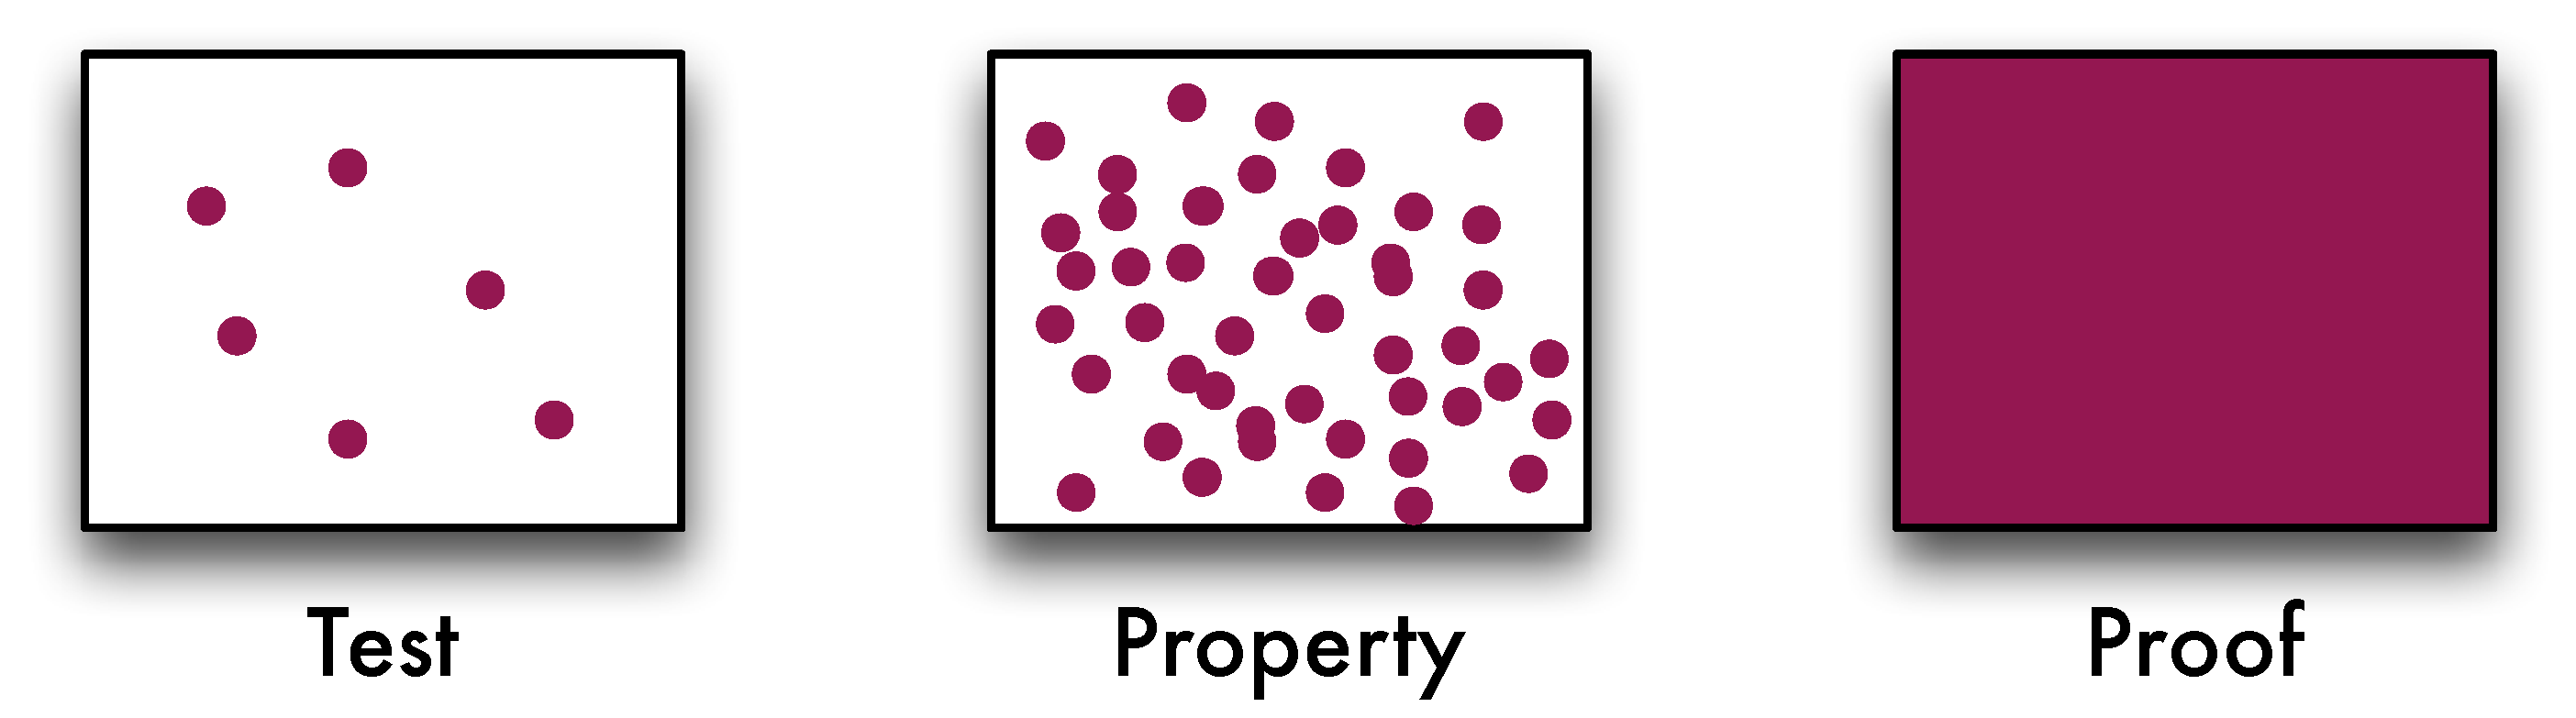
\includegraphics[width=4in]{Pictures/TestPropertyProof.pdf}
\end{center}
\caption{Coverage of testing, property-based testing and proof}
\label{TPP}
\end{figure}

These properties are just like the tests, except that they are applied to an arbitrary \texttt{pic} rather than the \texttt{horse}. If we apply \texttt{quickCheck} to these properties like this
\begin{alltt}
quickCheck prop_rotate
\end{alltt}
and evaluate this in Haskell, we get the result
\begin{alltt}
+++ OK, passed 100 tests.
\end{alltt}
for the first two tests. In the final test we've replicated the error from earlier on, and we get this output
\begin{alltt}
*** Failed! Falsifiable (after 3 tests and 3 shrinks):  
["ab"]
\end{alltt}
This tells us two things: it tells us that the property isn't always true, and it also gives us an example of when it goes wrong. In fact we get the simplest case where it goes wrong, through ``shrinking'':\index{property-based testing!shrinking} this is a picture with one line and two characters!

This testing is automatic: once we have written the properties to test, the data are generated randomly from the type -- \texttt{Picture} in this case. Through the book we'll see more complex examples of using QuickCheck, and find ways that we can control how QuickCheck works. 

\subsection*{Coverage}
\index{testing!coverage}

Property-based testing has replaced one test with a hundred, but we might still be unlucky, and miss the failing cases in the random data. On the other hand, having a proof gives us complete certainty that a function is correct. 

Figure \ref{TPP} illustrates the coverage given by the different mechanisms. Testing will check how the program behaves at a few, well-chosen, points; property-based testing expands this to hundreds of randomly-generated points, which, it is hoped, are representative, but a point where an error occurs \emph{may} be missed\footnote{We'll see an example of this in Chapter \ref{reasoningProgs}}; proof covers \emph{all} cases, no exceptions.

\subsection*{Proof}
\index{proof|(}

A \textbf{proof} is a logical or mathematical argument to show that something
holds {\em in all circumstances}. For example, given any particular
right-angled triangle
\begin{center}
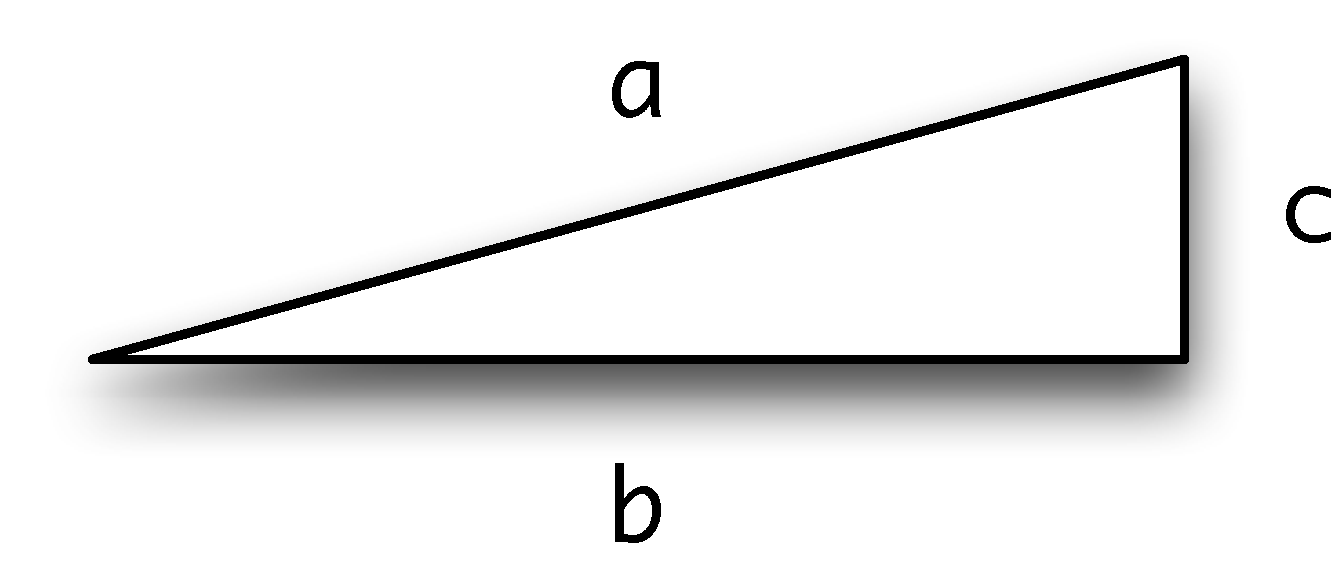
\includegraphics[width=2.0in]{Pictures/pythag.pdf}
\end{center}
we can check whether or not \texttt{a$^{\tt 2}$=b$^{\tt 2}$+c$^{\tt 2}$} holds. 
\index{Pythagoras's theorem} In each case we check,
this formula will hold, but this is not in itself enough to show that the
formula holds for all \texttt{a}, \texttt{b} and \texttt{c}. A proof of Pythagoras's Theorem, on the other hand, is a general
argument which establishes that \texttt{a$^{\tt 2}$=b$^{\tt 2}$+c$^{\tt 2}$} holds whatever
right-angled triangle we choose.

How is proof relevant to functional programming? To answer this we go back to the example of flipping in horizontal and vertical mirrors. As we saw in Figure \ref{vh-hv}, the order of reflection looks as though is not significant, and we can express this as the property:
\begin{alltt}
prop_rotate :: Picture -> Bool
prop_rotate pic  =  flipV (flipH pic) == flipH (flipV pic)
\end{alltt}\minx{prop\_rotate} 
Moreover, we can look at our implementations of
\texttt{flipV} and \texttt{flipH} and give a logical
\textbf{proof}\index{proof} that these functions have the property
\texttt{prop\_rotate} above for \textbf{any} picture \texttt{pic}. The crux of the argument is that the two
functions operate independently:
\begin{itemize}
\item the function \texttt{flipV} affects each line but leaves the lines
in the same order while
\item the function \texttt{flipH} leaves each line unaffected, while
reversing the order of the list of lines.
\end{itemize}
Because the two functions affect different aspects of the list it is
immaterial which is applied first, since the overall effect of applying
the two in either case is to
\begin{itemize}
\item reverse each line and
reverse the order of the list of lines.
\end{itemize}
Proof is possible for most programming languages, but
it is substantially easier for functional languages than for any other
paradigm. Proof of program properties will be a theme in this text, and
we start by exploring proof for list-processing functions in Chapter
\ref{reasoningProgs}.

What benefit is there in having a proof of a property like \texttt{prop\_rotate}?
It give us {\em certainty\/} that our functions have a particular property. 
Contrast this with traditional and property-based testing. In both cases 
the test only gives us the assurance
that the function has the property we seek at the test points, and in principle tells us
nothing about the function in other circumstances. There are
safety-critical situations in which it is highly desirable to be sure
that a program behaves properly, and proof 
has a role here. We
are not, however, advocating that testing is unimportant -- merely that testing
and proof have complementary roles to play in software development. 
 

More specifically, \texttt{prop\_rotate} means that we can
be sure that whatever order we apply the functions \texttt{flipH} and 
\texttt{flipV} they will have the same effect. We could
therefore \textbf{transform}\index{program transformation} a program containing \texttt{...\ (flipH\ (flipV\ ...))\ ...}
into one using the functions in the reverse order,  \texttt{...\ (flipV\ (flipH\ ...))\ ...}, and be certain that the new
program will have exactly the same effect as the old. Ideas like this can be
used to good effect within implementations of languages, and also in
developing
programs themselves, as we shall see in Section \ref{verifGen}.
\index{proof|)}



\begin{summary}
As we said at the start, this chapter has three aims. We wanted to
introduce some of the fundamental ideas of functional programming; to
illustrate them with the example of pictures, and also to give a flavour
of what it is that is distinctive about functional programming.
To sum up the definitions we have seen,
\begin{itemize}
\item a function\index{function} is something which transforms its inputs
to an output;
\item a type\index{type} is a collection of objects of similar sort, such as
 whole numbers (integers)  or pictures;
\item every object has a clearly defined type, and we state this type on
making a definition;
\item functions defined in a program are used in writing expressions to
be evaluated by the implementation; and
\item the values of expressions can be found by
performing calculation by hand, or by using GHCi.
\end{itemize}
In the remainder of the book we'll explore different ways of defining new types
and functions, as well as
following up the topics of polymorphism, functions as arguments and results, data
abstraction and proof which we have touched upon in an informal way
here.
We'll also make sure that we validate our programs using property-based testing in QuickCheck as well as proof. Finally, we'll see how Haskell is used in defining domain-specific languages.
\end{summary}
%\end{document} 




%\documentclass{book}\usepackage{sjtfonts}\usepackage{includegraphics}\usepackage{alltt}\usepackage{latexsym}
%\begin{document}\input{defs0}%		miradefs.tex 		    June 1994

% opening and closing a quoted Miranda section

\newcommand{\mira}{\noindent\hrulefill\nopagebreak\so}
\newcommand{\arim}{\nopagebreak\st\hrulefill\\}

% backslash in the Miranda environment
% Only feasible approach is to use \verb+\+
% in line!

%\newcommand{\bs}{$\mi\backslash\!\!$}
%\newcommand{\lbs}{\mbox{\verb+\+}}

% ignoring part of the input

\newcommand{\ignore}[1]{}

% a blank line in a Miranda section

\newcommand{\bl}{\mbox{\ }}

% Signalling a diffculty.

\definecolor{light-gray}{gray}{0.95}

\newcommand{\beware}[2]
 {\medskip\noindent\colorbox{light-gray}{\parbox{\textwidth}
 {\mbox{\large\textbf{#1}} \medskip\noindent\\ #2}\medskip\noindent}}

% Subscripting in Miranda text
\newcommand{\subscr}[2]{\mbox{${\mbox{\texttt{#1}}}_{\mbox{\texttt{#2}}}$}}

%\newcommand{\subscr}[2]{\mbox{${\mbox{\mi #1}}_{\mbox{\smtt #2}}$}}
\newcommand{\aone}{\subscr{a}{1}}
\newcommand{\atwo}{\subscr{a}{2}}
\newcommand{\ak}{\subscr{a}{k}}

\newcommand{\aoneone}{\subscr{a}{1,1}}

\newcommand{\eone}{\subscr{e}{1}}
\newcommand{\etwo}{\subscr{e}{2}}
\newcommand{\ei}{\subscr{e}{i}}
\newcommand{\er}{\subscr{e}{r}}

\newcommand{\fone}{\subscr{f}{1}}
\newcommand{\fl}{\subscr{f}{l}}

\newcommand{\gone}{\subscr{g}{1}}
\newcommand{\gtwo}{\subscr{g}{2}}
\newcommand{\gi}{\subscr{g}{i}}
\newcommand{\gr}{\subscr{g}{r}}

\newcommand{\hone}{\subscr{h}{1}}
\newcommand{\hl}{\subscr{h}{l}}

\newcommand{\pone}{\subscr{p}{1}}
\newcommand{\ptwo}{\subscr{p}{2}}
\newcommand{\pk}{\subscr{p}{k}}

\newcommand{\qone}{\subscr{q}{1}}
\newcommand{\qtwo}{\subscr{q}{2}}
\newcommand{\qk}{\subscr{q}{k}}

\newcommand{\rone}{\subscr{r}{1}}
\newcommand{\rtwo}{\subscr{r}{2}}

\newcommand{\tone}{\subscr{t}{1}}
\newcommand{\ttwo}{\subscr{t}{2}}
\newcommand{\tn}{\subscr{t}{n}}

\newcommand{\vone}{\subscr{v}{1}}
\newcommand{\vtwo}{\subscr{v}{2}}
\newcommand{\vn}{\subscr{v}{n}}

% for regular expressions

\newcommand{\stone}{\subscr{st}{1}}
\newcommand{\sttwo}{\subscr{st}{2}}
\newcommand{\stn}{\subscr{st}{n}}
\newcommand{\rthree}{\subscr{r}{3}}

\newcommand{\eps}{$\varepsilon$}
\newcommand{\trans}[1]{\stackrel{\mbox{\tt #1}}{\longrightarrow}}



% superscript in Miranda text

\newcommand{\superscr}[2]{\mbox{${\mbox{\mi #1}}^{\mbox{\smtt #2}}$}}

% Not equals in Miranda text

\newcommand{\noteq}{\makebox[0pt][l]{=}/}
\newcommand{\overslash}{\makebox[0pt][l]{/}}

% Definitions in complexity chapter

\newfont{\oldSym}{cmsy10}
\newcommand{\Th}{\boldmath$\oldSym\Theta$}
\newcommand{\pow}[1]{\^{}#1}
\newcommand{\leqq}{$\leq$}
\newcommand{\geqq}{$\geq$}
\newcommand{\lll}{$\ll$}
\newcommand{\eqq}{$\equiv$}
\newcommand{\ltwo}{\subscr{log}{2}}

% Indexing

\newcommand{\minx}[1]{\index{#1@{\ttfamily{}#1}}}



\chapter{Getting started with Haskell programming}
\label{getStart}
\chapstart

\medskip
Chapter \ref{intro} introduced the foundations of functional programming in Haskell.
We are now ready to use GHCi to do some practical programming, and we introduce it here.

In beginning to program we will also learn the basics of the Haskell module 
system, under which programs can be written in multiple, interdependent files, 
and which can use the `built-in' functions in the prelude and libraries. 
Our programming
examples will concentrate on using the \texttt{Picture} example
introduced in Chapter \ref{intro} as well as some simple numerical
examples. 

In support of this we will look at how to get hold of the programs and
other background materials for the book from Hackage using Cabal, as well as how to obtain and install GHCi using GHCup. We will explore how to develop single-module programs using \texttt{ghci} as well as using \texttt{cabal repl} for more complex, multiple module projects.

We conclude by briefly surveying the kinds of error message that can
result from typing something incorrect into GHCi. 

\begin{figure}[t]
\begin{alltt}\minx{FirstScript.hs}
\input{FirstScript.hs}
\end{alltt}
\vspace*{-12pt}
\caption{An example script, \texttt{FirstScript.hs}.}
\label{FirstScript}
\end{figure}

\section[A first Haskell program]{A first Haskell program}
\markright{A first Haskell program}
 
We begin the chapter by giving a first Haskell program or
\textbf{script}\index{script}, which consists of the numerical examples from
Chapter \ref{intro}. This is the file
\texttt{FirstScript.hs}, shown in Figure \ref{FirstScript}. Haskell scripts are stored in files with the \textbf{extension}\index{extension}
`\texttt{.hs}'.\index{hs@\texttt{.hs}}





As well as definitions, a script will contain comments. 
A \textbf{comment}\index{comment} in a script
is a piece of information of value to a human reader rather than to a computer.
It might contain an informal explanation of how a function works,
how it should or should not be used, the overall design philosophy of a library and so on.
Everything in a program file is interpreted as
program text, \emph{except} where it is explicitly indicated that it is a
comment. 

Comments are indicated in two ways. The symbol
`\texttt{-{}-}'\minx{--} begins a comment\index{comment!symbol} which occupies the part of the
line to the right of the symbol. Comments can also be enclosed by the 
symbols `\texttt{\{-}'\minx{\{-} and `\texttt{-\}}'\minx{-\}}. These comments can be of
arbitrary length, spanning more than one line, as well as enclosing other comments; 
they are therefore
called \textbf{nested comments}\index{comment!nested}.

\section{Using Haskell in practice}
\index{GHCi|(}

The Glasgow Haskell Compiler (GHC)\index{Glasgow Haskell Compiler|see{GHC}}\index{GHC} is an industrial-strength compiler for Haskell. \textbf{GHC interactive (GHCi)} is an interactive interpreter based on GHC, which provides programmers with a Haskell \textbf{repl}, which successively \emph{reads} an expression, \emph{evaluates} it, \emph{prints} the result, and finally \emph{loops} back to the start. This is a great way to start programming, as it allows you to try out your ideas and experiment with definitions in the process of developing a program.

If you're learning Haskell in high school or college, or at work, your teachers or colleagues will have made sure it is available on the computers you use. If you want to install it for yourself on a machine that you control, the best, and easiest, way of working doing that is to use GHCup, \url{https://www.haskell.org/ghcup/}.

\begin{figure}[t] 
\begin{center}
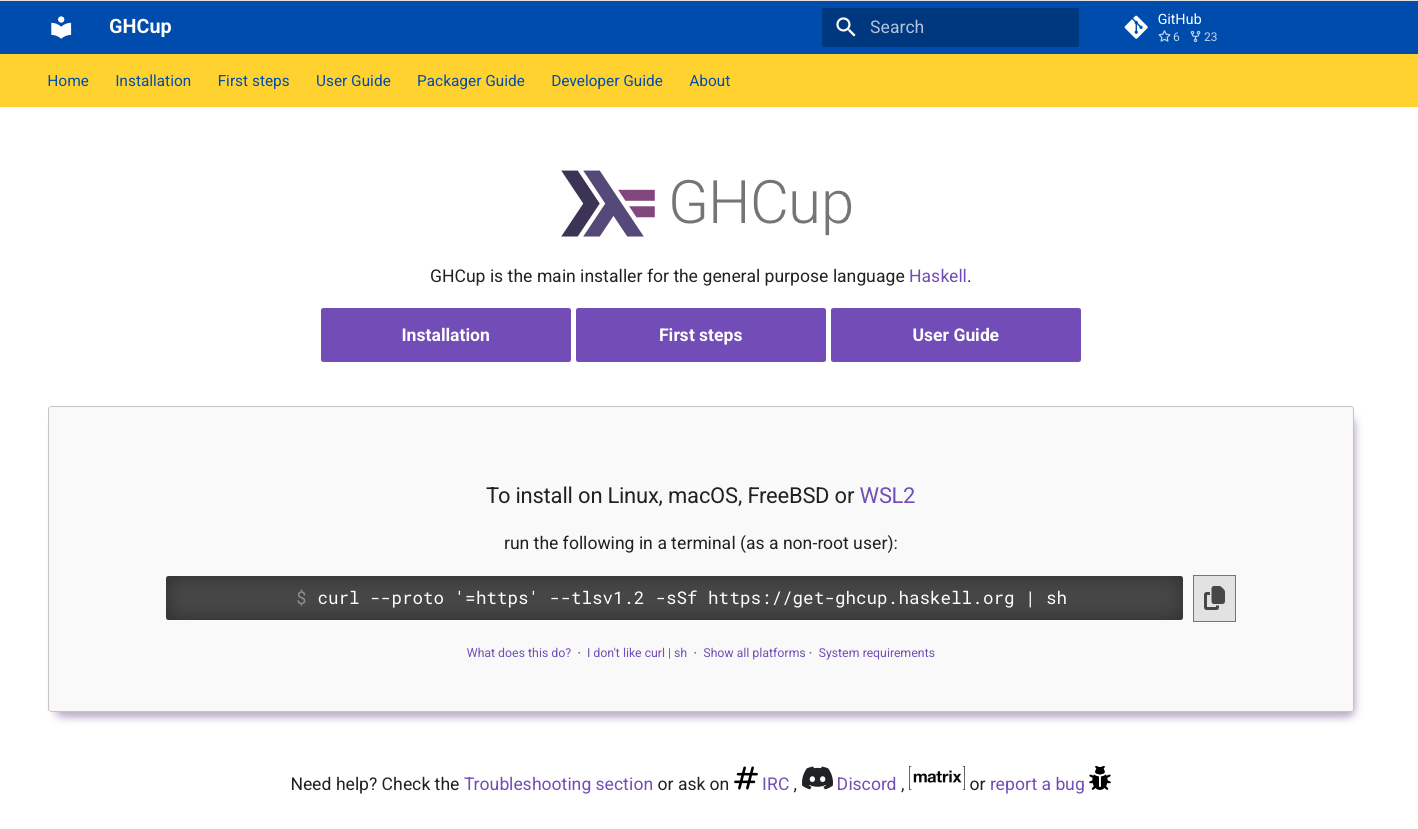
\includegraphics[width=\textwidth]{Pictures/GHCup.png}
\end{center} 
\caption{The GHCup homepage}
\label{GHCup}
\end{figure}

GHCup\index{GHCup} will install GHC, as well as some other components including \texttt{cabal},\index{Cabal} which is a package for distributing Haskell code and libraries, and one of the ways that you can access the code for the book;\index{downloading support materials}. If asked to select what to download, include \texttt{cabal}, and if you want to use Haskell within an IDE like VS Code, include the Haskell Language Server (HLS)\index{Haskell Language Server}\index{HLS} too. Also, you should follow the GHCup default of installing the \emph{recommended} versions of these programs.

Why should you consider using HLS? Development today is usually inside an Integrated Development Environment, or IDE, such as Visual Studio Code (VS Code). IDEs combines
editing with processing and running programs, as well as interacting with reposito-
ries, such as github, refactoring and other kinds of software tooling. To use Haskell most effectively within an IDE you will need to use the Haskell Language Server (HLS), which provides a rich enhancement of the editing functions of the IDE including type checking, refactoring,  integration with repositories and other support for software development.

We will come back to \texttt{cabal} and HLS when we discuss multi-file projects in Section \ref{multipleModuleProgs} and again when we discuss how to find out more about the functions and libraries in Haskell in Chapter \ref{progLists}.



 
Other ways of using Haskell -- such as using it online or in a browser -- can be found in Appendix \ref{OtherHS}.


\begin{figure}[t] 
\begin{center}
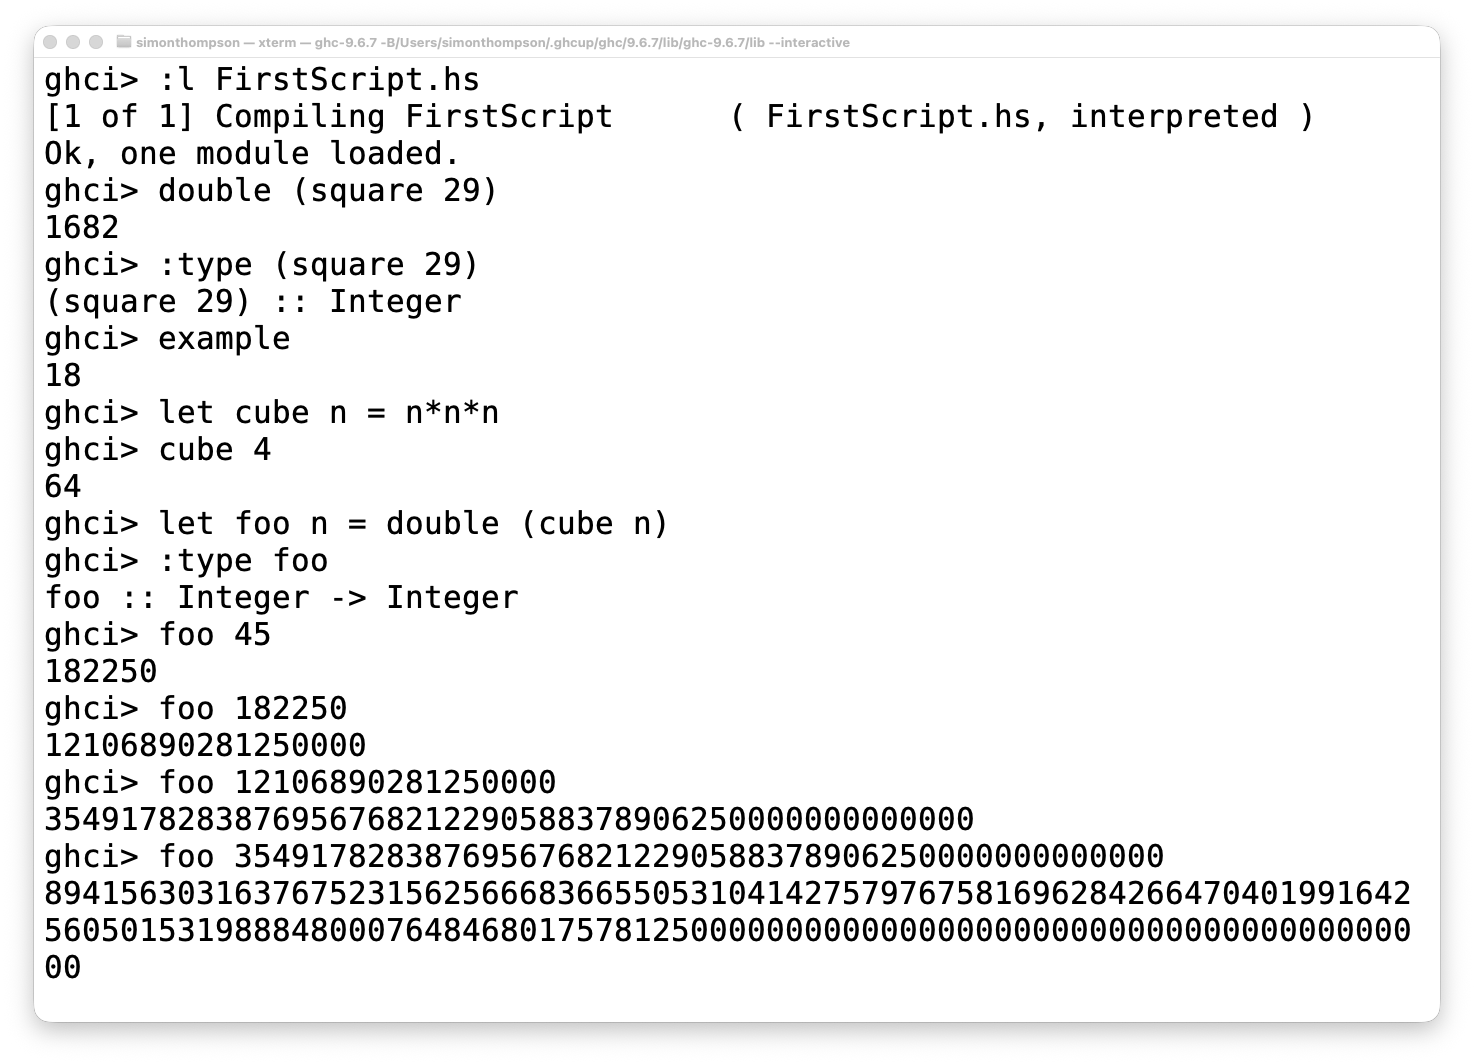
\includegraphics[width=\textwidth]{Pictures/ghci-terminal.png}
\end{center} 
\caption{A GHCi terminal session}
\label{GHCiSession}
\end{figure}


\section{Using GHCi}


In this text we describe the terminal-style interface to GHCi, illustrated in Figure
\ref{GHCiSession},
because this is common to macOS, Linux and Windows WSL. 

\subsection*{GHCi documentation}
\index{GHCi!documentation}

The GHCup webpage has documentation about `first steps' in getting started, covering \texttt{ghci} after a short introduction to the \texttt{ghc} command itself.
\begin{center}\index{GHCup!first steps}
\url{https://www.haskell.org/ghcup/steps/}
\end{center} 
The full documentation for the Glasgow Haskell Compiler is here
\begin{center}\index{GHCi!documentation}
\url{https://downloads.haskell.org/ghc/latest/docs/users_guide/}
\end{center} 
and that includes information specifically about GHCi.


\subsection*{Starting GHCi}

To start GHCi in a terminal on macOS, Linux and WSL, type \texttt{ghci}\minx{ghci}
to the prompt in a terminal. To launch GHCi using a particular file, change to the directory containing the file and type
\texttt{ghci} followed by the name of the file in question, as in
\begin{alltt}\minx{ghci}
ghci Chapter2
\end{alltt} 
Haskell scripts carry the extension \texttt{.hs}; only such files can be loaded, and their extensions
can be omitted when they are loaded either when GHCi is launched or by a
\texttt{:load}\index{load@\texttt{:load}} command within GHCi.

\subsection*{Evaluating expressions in GHCi}
\index{GHCi!expression evaluation}

As we said in Section \ref{exprEval}, GHCi will evaluate
expressions typed at the prompt. We see in Figure \ref{GHCiSession} the
evaluation of \texttt{double (square 29)} to \texttt{1682}, like this
\begin{alltt}
\textsl{ghci>} double (square 29)
\textsl{1682}
\textsl{ghci>}
\end{alltt}
where we have indicated the machine output by using a slanted font; user input appears
in unslanted form. The \textbf{prompt}\index{prompt} here, \texttt{\textsl{ghci>}}, will be explained in
Section \ref{introModules} below.\minx{ghci>}
As can be seen from the examples, we can evaluate expressions which use
the definitions in the current script. In this case it is \texttt{Chapter2.hs}.

One of the advantages of the GHCi repl interface is that it is easy to
experiment with functions, trying different evaluations simply by typing
the expressions at the keyboard. If we want to evaluate a complex
expression, we could add it to the program, as in this 
definition
\begin{alltt}
cube :: Integer -> Integer
cube n = n*n*n
\end{alltt}
but we can also input these definitions directly into GHCi by prefacing them with the keyword \texttt{let}, as seen in Figure \ref{GHCiSession}. Of course, this definition will be lost when we close GHCi, so if we want to keep a record of it, then we should add it to a Haskell module as well.

\newlength{\colwidth}
\setlength{\colwidth}{\textwidth}
\addtolength{\colwidth}{-1.9in}

\begin{figure}[t]
\begin{tabular*}{\textwidth}{p{2in}p{0.3in}p{\colwidth}}
\textbf{Command} & \textbf{Abbrev.} & \textbf{Action} \\ \  \\
\texttt{:load Parrot}\index{load@\texttt{:load}} & \texttt{:l} & Load the Haskell module \texttt{Parrot.hs}; the file extension \texttt{.hs} can be omitted.\\
\texttt{:reload}\index{reload@\texttt{:reload}} & \texttt{:r} & Repeat the last \texttt{:load} command.\\
\texttt{:type exp}\index{type@\texttt{:type}} & \texttt{:t} & Give the type of the expression \texttt{exp}; e.g. typing
\texttt{:type size+2}\ \ gives\ \ \texttt{size+2 ::\ Integer}.\\
\texttt{:info name} \index{info@\texttt{:info}}& \texttt{:i} & Give information about the thing called
\texttt{name}.\\
\texttt{:browse Name} \index{browse@\texttt{:browse}}& & Give information about the definitions in the module
\texttt{Name}, if it is loaded.\\
\texttt{:quit}\index{quit@\texttt{:quit}} & \texttt{:q} & Quit the system.\\
\texttt{:help}\minx{:?}\index{GHCi!help} & \texttt{:h,:?} & Give a complete list of the GHCi commands.\\
\texttt{:!\ command} & & Escape to perform a Unix or DOS \texttt{command}.\\
\texttt{:edit First.hs} \index{edit@\texttt{:edit}}& \texttt{:e} & Edit the file
\texttt{First.hs} in the default editor. Note that the file 
extension \texttt{.hs} is
needed in this case. See the following section for more information on editing.\\
\texttt{:set editor vi} \index{set@\texttt{:set}}& \texttt{:s} & Set the \texttt{editor} to be \texttt{vi}.\\
\ensuremath{\uparrow}, \ensuremath{\downarrow} &  & Move up (\ensuremath{\uparrow}) and down (\ensuremath{\downarrow}) the command history.\\
\ensuremath{\rightarrow\!\!\mid} &  & Name and command completion: complete module or file names, or GHCi commands.\\
\texttt{let s = exp}\minx{let} & & Give \texttt{s} the value of \texttt{exp} within this GHCi session.
\end{tabular*}\index{GHCi!commands!shortened form} 
\caption{Principal GHCi commands}
\label{commands}
\end{figure}

\subsection*{GHCi commands}
\index{GHCi!commands}

GHCi commands begin with a colon, `\texttt{:}'.\minx{:} A summary of the
main commands is given in Figure \ref{commands}.
When a GHCi command can be abbreviated to their initial letter this is shown in the table in Figure \ref{commands}.
Outline information about other commands is given by the \texttt{:help} command, and comprehensive details can be
found in the
on-line GHCi documentation discussed above.

\subsection*{Editing scripts}
\index{GHCi!editing}

GHCi can be connected to a default text editor, so that GHCi commands such
as \texttt{:edit} use this editor. This may well be
determined by your local set-up (e.g. in the \texttt{EDITOR} variable),\minx{EDITOR} or can be set using the \texttt{:set} command in GHCi. 

Using the GHCi \texttt{:edit} command causes the editor to be invoked on
the appropriate file. When the editor is quit, the updated file is
loaded automatically. However, it can be more convenient to keep the editor running in
a separate window and to reload the file by:
\begin{itemize}
\item writing the updated file from the editor (without quitting it),
and then
\item reloading the file in GHCi using \texttt{:reload} or \texttt{:reload filename}.
\end{itemize}
In this way the editor is still open on the file should it need further
modification.


%Alternatively some editors allow GHCi to be called from within the editor, as a part of the Haskell mode for the editor. A popular Haskell editor is emacs, with variants such as Aquamacs for Mac OS X.\index{emacs, Haskell mode for}\index{Aquamacs|see{emacs}} These editors will provide facilities such as syntax highlighting, and embedded evaluation. In Haskell mode for emacs, \texttt{\^\-C \^\-B} opens GHCi and \texttt{\^\-C \^\-L} (re)loads the current module in GHCi.



\subsection*{A first GHCi session}
\index{GHCi!first session}
Let's get started with GHCi by doing some introductory exercises.

\subsubsection*{Task 1}
Load the file \texttt{FirstScript.hs} into GHCi, and evaluate 
the following expressions
\begin{alltt}
square size
square
double (square 2)
it
square (double 2)
let d = double 2
square d
23 - double (3+1)
23 - double 3+1
it + 34
13 `div` 5
13 `mod` 5
\end{alltt}
On the basis of this can you work out the purpose of \texttt{it}\minx{it} and \texttt{let}\minx{let}?

\medskip
\noindent
\subsubsection*{Task 2}
Use the GHCi command \texttt{:type} to tell you the type of each of these, 
apart from \texttt{it}.

\medskip
\noindent
\subsubsection*{Task 3}
What is the effect of typing each of the following?
\begin{alltt}
double 2 3
double square
2 double
\end{alltt}
Try to give an explanation of the results that you obtain.

\medskip
\noindent
\subsubsection*{Task 4}
Edit the file \texttt{FirstScript.hs} to include
definitions of functions from integers to integers which behave
as follows.
\begin{itemize}
\item The function should double its input and square the result of
that.
\item The function should square its input and double the result of
that.
\end{itemize}
Your solution should include declarations of the types of the
functions.

\begin{figure}[t]
\beware{\texttt{let} in GHCi}{\minx{let}
It is possible to make \emph{temporary} definitions in GHCi using \texttt{let} like this:
\begin{alltt}
let s = 23
\end{alltt}
and once you have done this you can use \texttt{s} in any expressions you evaluate. You can define any Haskell value this way, too.

\medskip
Beware! These definitions are lost if you redefine \texttt{s} or when you leave GHCi, so it often best  to put definitions into a file, so that they are saved and you can edit them subsequently.}
\end{figure}

\index{GHCi|)}

\section{The standard prelude and the Haskell libraries}
\label{prelLibs}

We saw in Chapter \ref{intro} that Haskell has various built-in types, such as 
integers and
lists and functions over those types, including the arithmetic functions and the list 
functions \texttt{map} and \texttt{++}. Definitions of these are
contained in a file, the \textbf{standard prelude}\index{standard prelude|see{\texttt{Prelude.hs}}},
\texttt{Prelude.hs}\minx{Prelude.hs}. When Haskell is used, the default is to load the
standard prelude, and this can be seen by trying the GHCi command 
\begin{alltt}
:browse Prelude
\end{alltt}
which will list the types of all the functions in the \texttt{Prelude.hs} module.

As Haskell has developed over the last decade, the prelude has also grown. In
order to make the prelude smaller, and to free up some of the names used
in it, many of the definitions have been moved into 
\textbf{standard libraries},\index{standard libraries} which can be included when they are
needed. We shall say more about these libraries as we discuss particular parts of
the language. 

As well as the standard libraries, there is a wealth of 
contributed libraries that support property-based testing, concurrency, functional animations and so forth; we will introduce the libraries that we need as we go along.
These libraries are available on \emph{Hackage},\index{Hackage} \url{https://hackage.haskell.org}, the main online package repository for Haskell, using the Cabal installation system.  
We will say something more about Cabal in Section \ref{multipleModuleProgs} and give an overview of more Haskell modules and libraries in Chapter \ref{progLists}.

\section{Modules}
\label{introModules}
\index{modules!introduction|(}

\begin{figure}[t]
\begin{center}
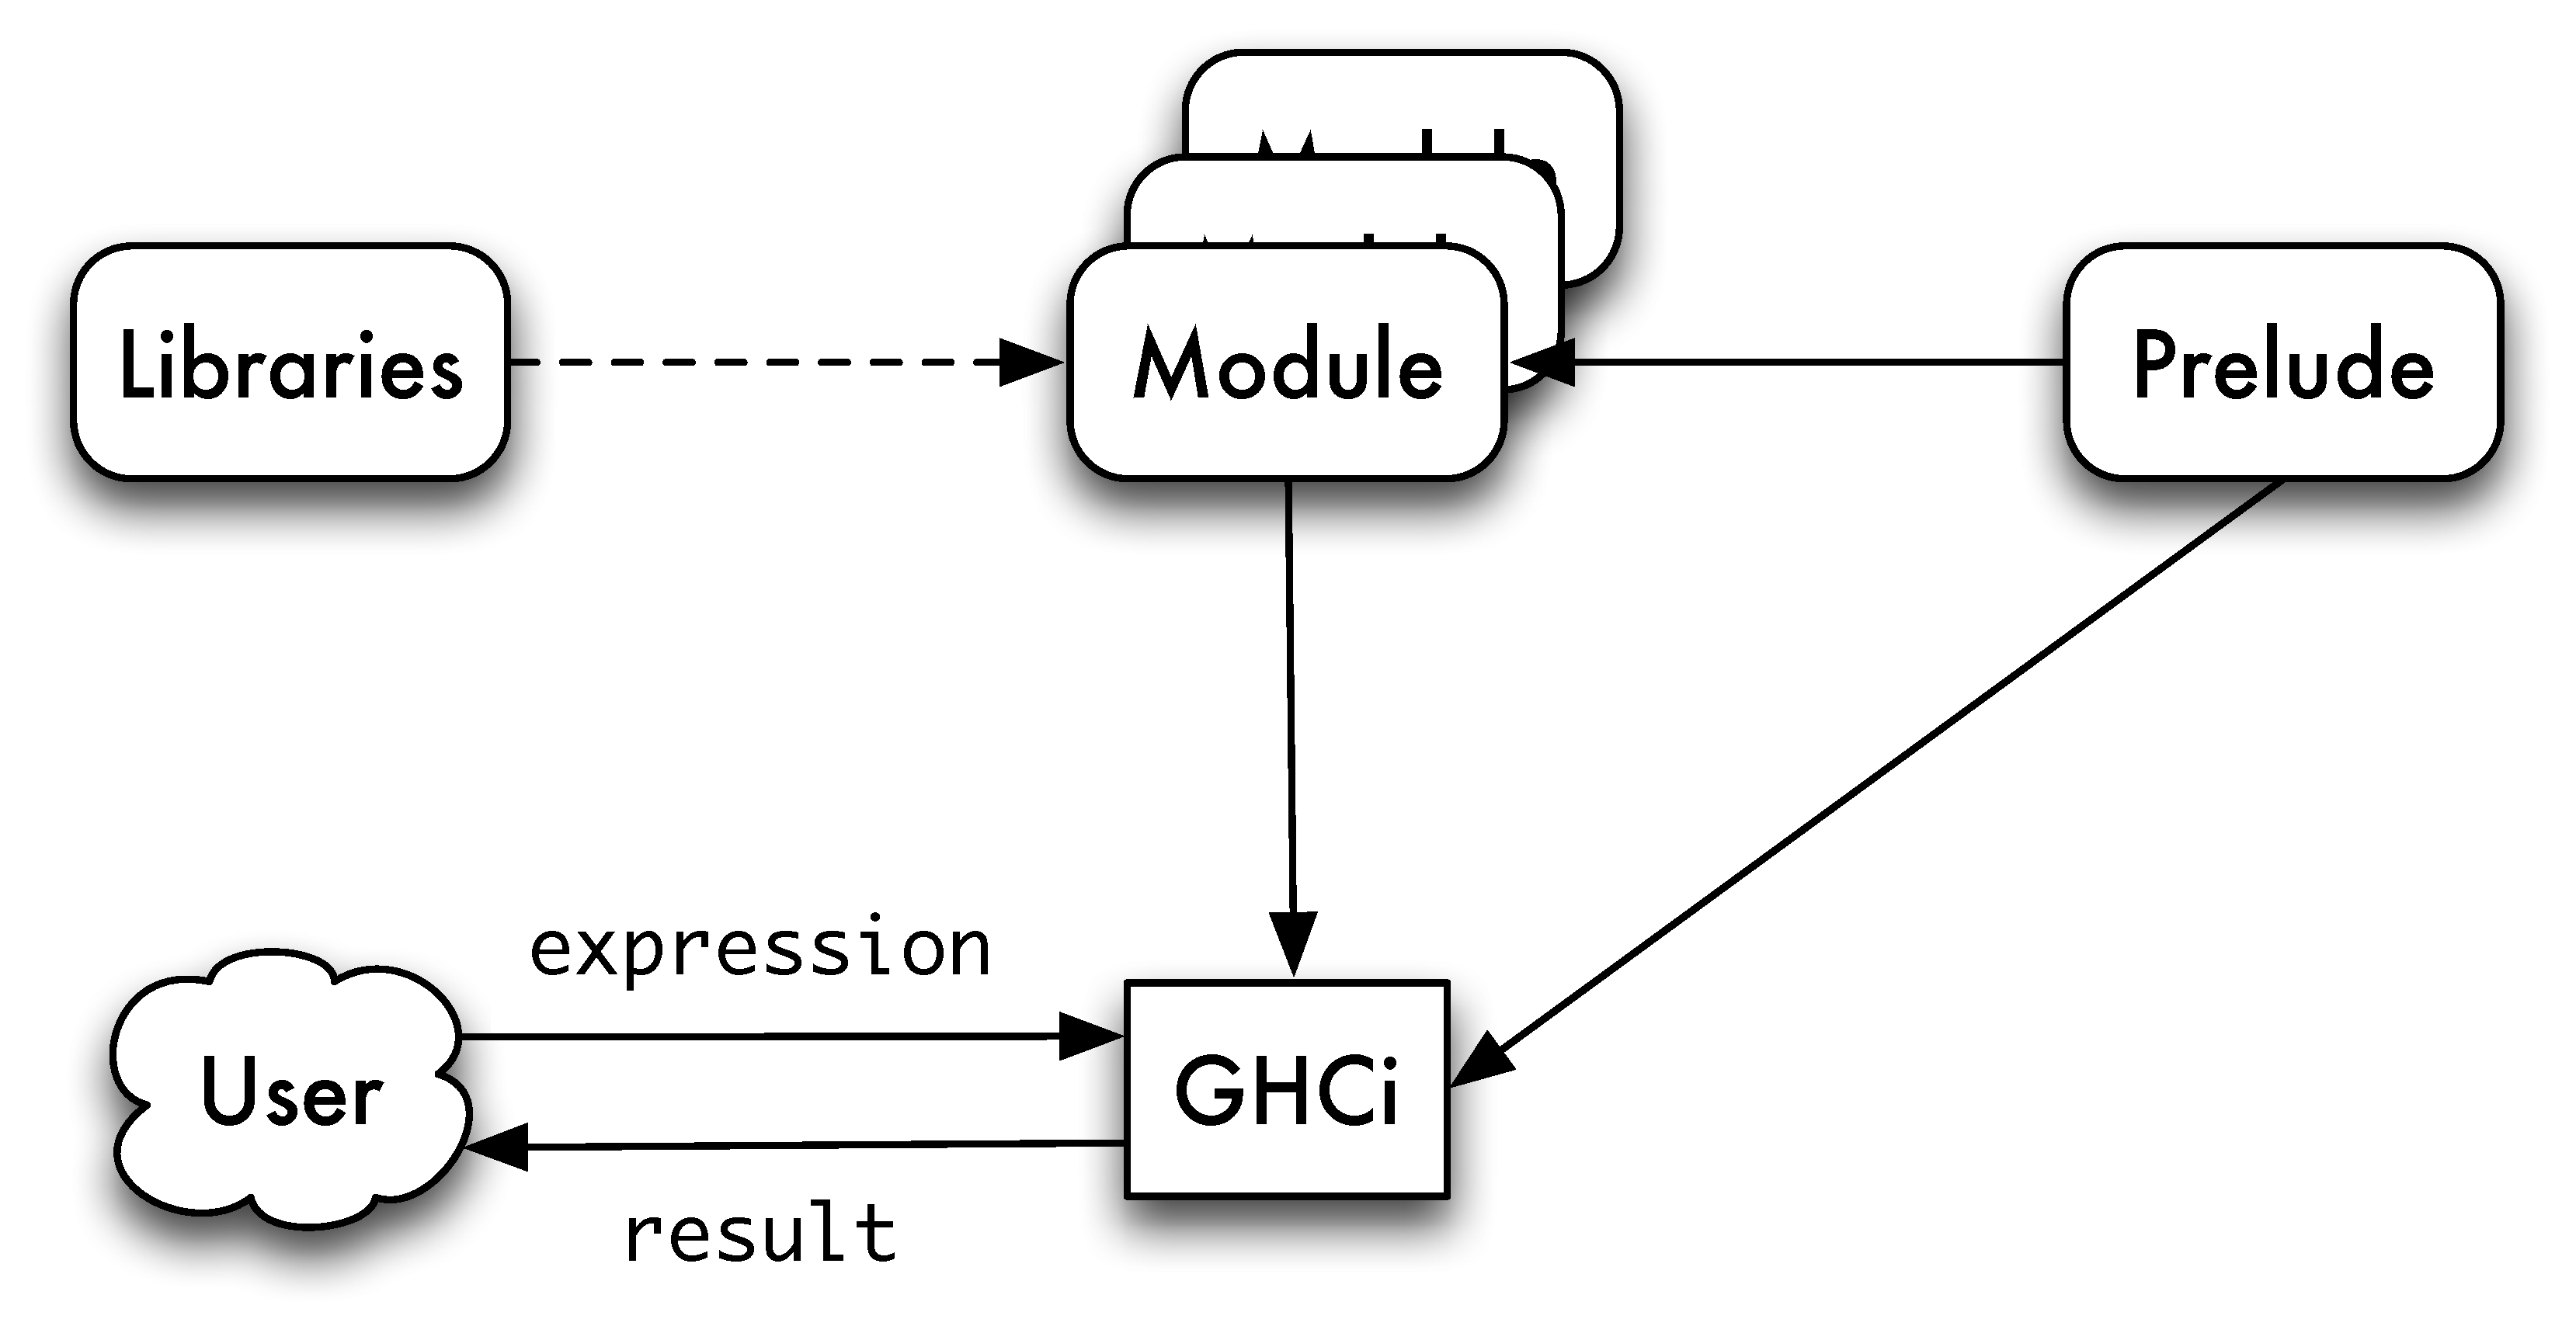
\includegraphics[width=4in]{Pictures/GHCiLibPrel.pdf}
\end{center} \index{GHCi!modules in}
\caption{GHCi, the Prelude and other modules}
\label{GHCiPreludeModules}
\end{figure}
 
A typical piece of computer software will contain thousands of lines of
program text. To make this manageable, we need to split it into smaller
components,  which we call modules. 

A \textbf{module}\index{modules} has a name
and will
contain a collection of Haskell definitions. To introduce a module called \texttt{Ant}
we begin the program text in the file thus:
\begin{alltt}\minx{Ant}\minx{module}
module Ant where
   ...
\end{alltt}
A module may also
\textbf{import}\minx{import} definitions from other modules. The module \texttt{Bee}
will import the definitions in \texttt{Ant} by including an \texttt{import} statement,
thus:
\begin{alltt}\minx{Bee}

module Bee where
import Ant
   ...
\end{alltt}
The import statement means that we can use all the definitions in
\texttt{Ant} when making definitions in \texttt{Bee}.
In dealing with modules in this text
we adopt
the conventions that
\begin{itemize}
\item there is exactly one module per file;
\item the file \texttt{Blah.hs} contains the module
\texttt{Blah}.
\end{itemize}
The module mechanism supports the libraries we discussed in
Section \ref{prelLibs}, but we can also use it to include code written by 
ourselves or someone else. 

The module mechanism allows us to control how definitions are imported
and also which definitions are made available or \textbf{exported}\minx{export} by a
module for use by other modules. We look at this in more depth in Chapter \ref{codes}, where we
also ask how modules are best used to support the design of software
systems.

In the light of what we have seen so far, Figure \ref{GHCiPreludeModules} illustrates a GHCi session.
like this: 
The current module will have access to the standard prelude, and to
those modules which it \texttt{imports}; these might include modules
from the standard libraries, which are found in the same directory as the
standard prelude\index{standard libraries!location of}. The user interacts with GHCi, providing
expressions to evaluate and other commands and receiving the results of
the evaluations.
\index{modules!introduction|)}

In the next section we look at how to work with multiple-module projects in GHCi, including the code for this text.

\section{Working with multiple-module projects}
\label{multipleModuleProgs}
\index{modules!multiple-module projects}

As we saw in the previous section, Haskell projects can be built from multiple modules, using the import and export mechanism. In this section we look at how projects can be downloaded and used; in particular how we can make sure that we're able to resolve all the dependencies of a particular project. We will see this in action with the Haskell package for this book, \texttt{Craft3e}.\index{Hackage!\texttt{Craft3e}}

Haskell projects, most of which consist of multiple modules, can be found on the Haskell Package Manager site, Hackage\index{Hackage}, and downloaded using Cabal\index{Cabal}. These projects themselves can depend on other packages, and this dependency and other \emph{project metadata} is contained in a \texttt{.cabal} file in the home directory of the package. The \texttt{.cabal} file summarises this information in a machine-readable format, allowing GHC to load all the dependencies of the project.

\subsection*{Working with \texttt{Craft3e}}

The code for this text is available on Hackage at 
\begin{center}
\url{https://hackage.haskell.org/package/Craft3e}
\end{center}
To download this to your machine type \texttt{cabal unpack Craft3e}. This will install the code for the book in a folder under \texttt{.cabal} in your home directory: the folder will be named \texttt{Craft3e-<version>}, where \texttt{<version>} is replaced by the current version number, \texttt{0.2.0.4} at the time of writing (2026-09-03).

Alternatively, if you are familiar with git and github, you can obtain the code from the github repository 
\begin{center}
\url{https://github.com/simonjohnthompson/haskellcraft}
\end{center}
by cloning the repository. As well as the code, this repository contains the source code for the book itself, and other miscellaneous material.

Whichever way you obtain the project, to work with the project, first change directory into the directory \texttt{Craft3e} (if you cloned the project from github) or \texttt{Craft3e-<version>} if you used \texttt{cabal unpack}. In either case you can then first run
\begin{alltt}
cabal build  
\end{alltt} 
which will install all the code that the book depends on; you just need to do this once, after obtaining the \texttt{Craft3e} project. Then to interact with the code in the project type
\begin{alltt}
cabal repl
\end{alltt}
This gives you a \texttt{ghci} prompt, but this time connected to GHC with all the dependencies available. You can work with ghci in the usual way.  The first time that you run \texttt{cabal repl} after obtaining the project may take time to complete, as the system installs dependencies: don't worry, this won't be a problem the next time you use it. 

Any new modules, such as \texttt{MyNewModule.hs} that you create \emph{within or below the Craft3e directory} will also have these dependencies available. These can be loaded with \texttt{:l MyNewModule}, and reloaded with \texttt{:r}, in the usual way.

If you choose to use an IDE such as VS Code you should open the Craft3e folder using the \textbf{Open Folder} command in the \textbf{File} menu. This will ensure that dependencies are visible, and the built-in terminal will be opened in the same directory. You can then use the Cabal commands just as they are described above.  VS Code is enhanced with HLS using the \texttt{haskell.haskell} extension, which is documented and downloadable from here:
\begin{center}
  \url{https://marketplace.visualstudio.com/items?itemName=haskell.haskell}
\end{center}
The next section revisits the picture example of Chapter
\ref{intro}, which is used to give a practical illustration of modules.


\begin{figure}[p]
\begin{alltt}\minx{Picture}
module Pictures where

type Picture = ....

-- The horse example used in Craft3e, and a white picture.

horse , white :: Picture
horse = ....
white = ....

-- Getting a picture onto the screen.

printPicture :: Picture -> IO ()
printPicture = ....

-- Reflection in vertical and horizontal mirrors.

flipV , flipH :: Picture -> Picture
flipV = map reverse
flipH = reverse

-- One picture above another. To maintain the rectangular 
-- property, the pictures need to have the same width.

above :: Picture -> Picture -> Picture
above = (++)

-- One picture next to another. To maintain the rectangular 
-- property, the pictures need to have the same height.

beside :: Picture -> Picture -> Picture
beside = zipWith (++)

-- Superimpose two pictures (assumed to be same size). 

superimpose :: Picture -> Picture -> Picture
superimpose = ....

-- Invert the black and white in the picture.

invertColour :: Picture -> Picture
invertColour = ....

\end{alltt}
\caption{A view of the \texttt{Pictures} module.}
\label{pictScript}
\vspace*{-12pt}
\end{figure}

\section{A second example: pictures}\label{picModuleEx}
\index{pictures}
\markright{A second example: \runinghead pictures}

The running example in Chapter \ref{intro} was of pictures, and we saw there that there are two implementations of these functions, one in \texttt{Pictures.hs} giving an `ASCII art' version, and the other in \texttt{PicturesSVG.hs} rendering pictures in a web browser.\minx{PicturesSVG}
\begin{itemize}\label{ShowBrowser}
\item
To use \texttt{PicturesSVG.hs}, open GHCi on this module like this:
\begin{alltt}\minx{ghci}
ghci PicturesSVG.hs
\end{alltt}
To show a picture in the browser, evaluate it using \texttt{render} as in \index{SVG!display in browser}
\begin{alltt}
render (horse `beside` (flipV horse))
\end{alltt}
This will give a browser display as shown in Figure \ref{svgpix}, page \pageref{svgpix}. The image in the browser will update automatically when you call \texttt{render} on another picture; if you would prefer to do this manually, use the file \texttt{showPic.html} instead.

\item
To use the `ASCII art' version, run
\begin{alltt}
ghci Pictures.hs
\end{alltt}
To show a picture in the terminal you need to use the function
\begin{alltt}\minx{printPicture}
printPicture :: Picture -> IO ()
\end{alltt}
which is used to display a \texttt{Picture} on the screen. The type
\texttt{IO} is a part of the Haskell mechanism for input/output
(I/O).\index{I/O}
We examine this mechanism in detail in Chapter \ref{io}; for
the present it is enough to know that if \texttt{horse} is the name of the
picture used in the earlier examples, then the effect of the function application
\texttt{\ printPicture horse\ } 
is the display
\begin{center}
{\footnotesize
\newlength{\blah}
\settowidth{\blah}{\texttt{............}}
\begin{minipage}{\blah}
\begin{alltt} 
.......##... 
.....##..#..
...##.....#.
..#.......#.
..#...#...#.
..#...###.#.
.#....#..##.
..#...#.....
...#...#....
....#..#....
.....#.#....
......##....
\end{alltt}
\end{minipage}
}
\end{center}
first seen in Chapter \ref{intro}. Any \texttt{Picture} can be printed
in a similar way. 
The \texttt{Pictures} module is shown in Figure \ref{pictScript}.
\end{itemize}
In the remainder of this section we present a series of practical
exercises designed to use either of the modules
\texttt{Pictures.hs} and \texttt{PicturesSVG.hs}.

\begin{exercises}

\item Define a module \texttt{UsePictures} which imports
\texttt{Pictures} (or \texttt{PicturesSVG}) and contains definitions of \texttt{blackHorse} and \texttt{rotateHorse} which can use the definitions
imported from the pictures module.

\medskip
\noindent
In the remaining questions you are expected to add other definitions to
your module \texttt{UsePictures}.

\item How could you make the picture
\begin{center}

\includegraphics[width=1in]{Pictures/twoByTwo.pdf}
\end{center}
Try to find two different ways of getting the result. It may help to work
with pieces of white and black paper.

Using your answer to the first part of this question, how would you
define a chess (or checkers) board, which is an $8\times8$ board of alternating squares? 

\item 
Three variants of the last picture which involve the `horse' pictures
are
\begin{center}
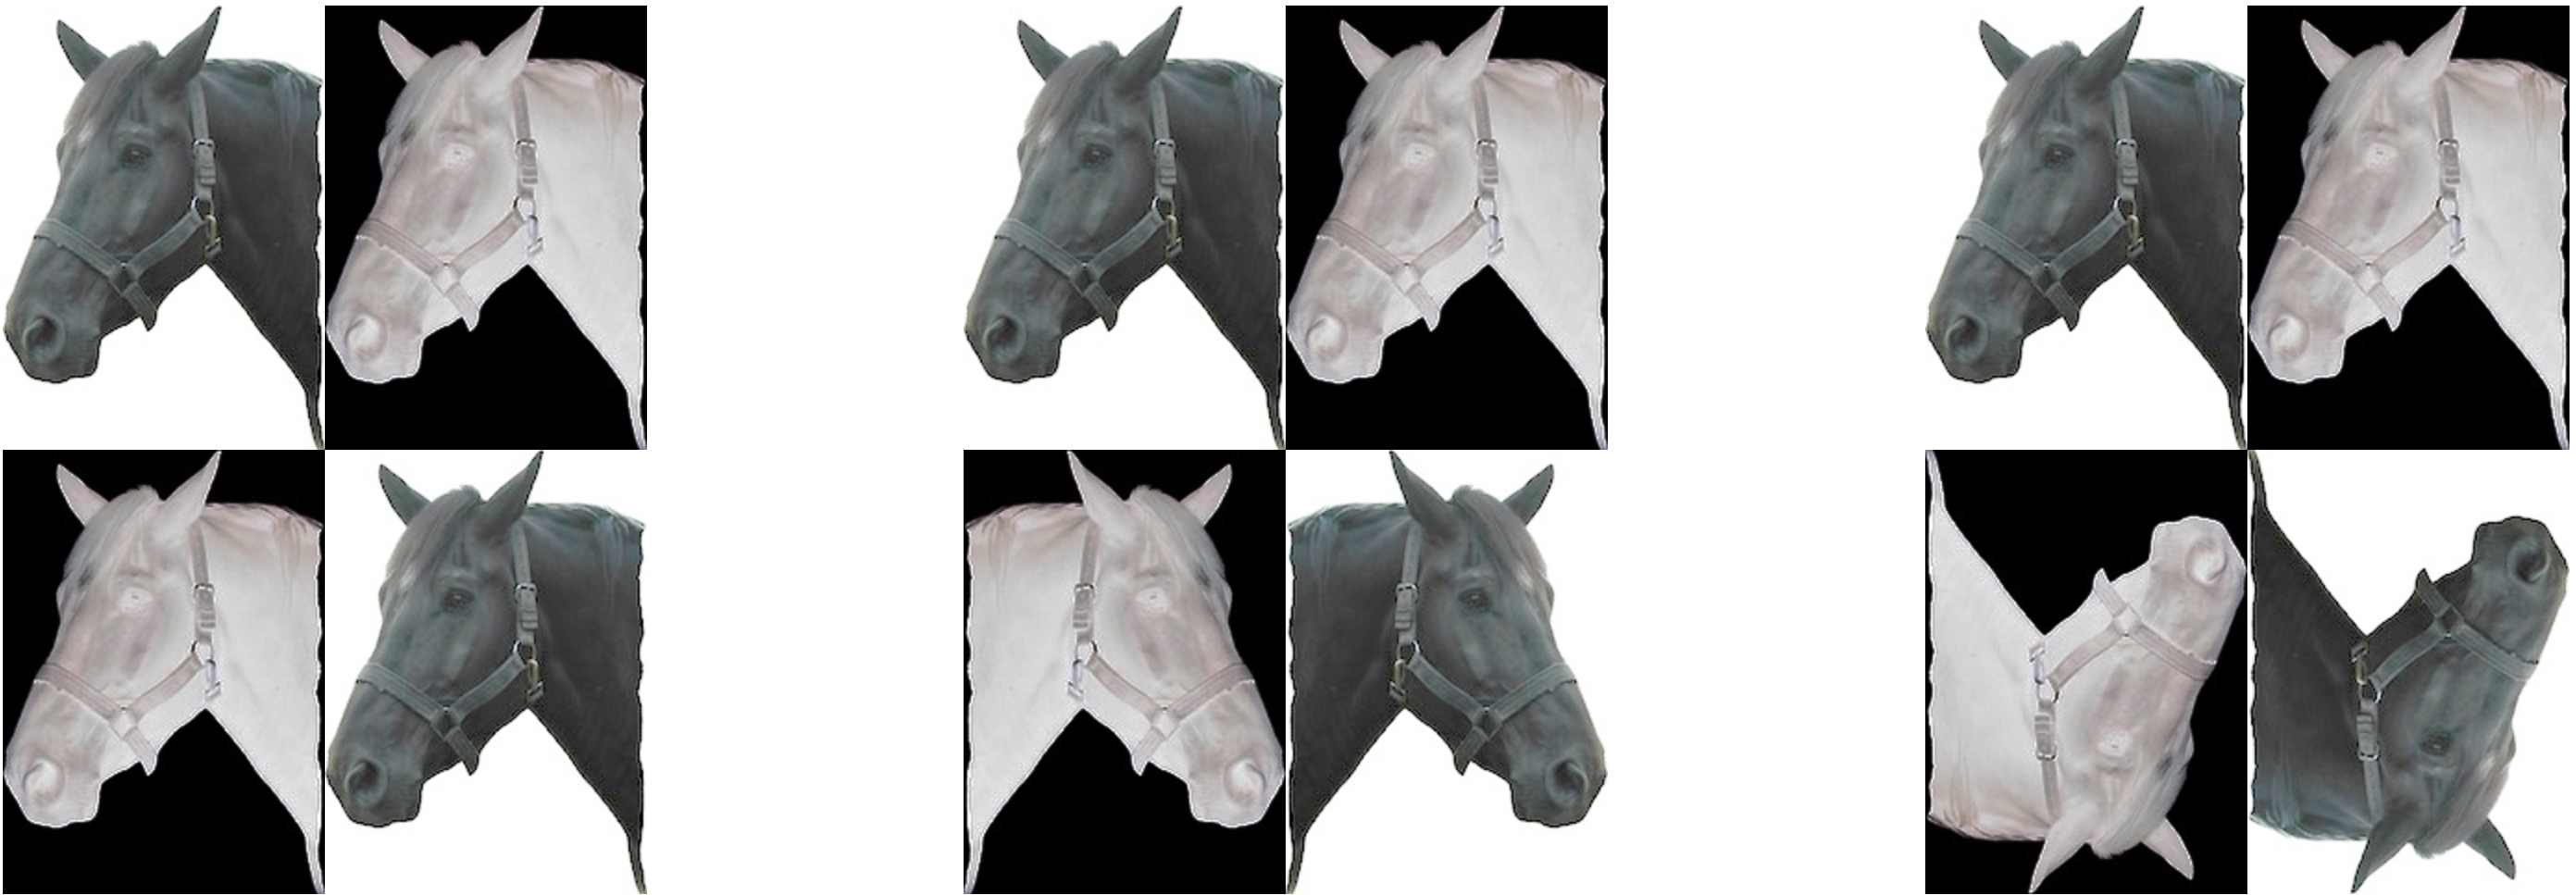
\includegraphics[width=4in]{Pictures/chessHorse.pdf}
\end{center}
How would you produce these three?

\item
Give another variant of the `horse' pictures in the previous question,
and show how it could be created. Note: a nice variant is 
\begin{center}
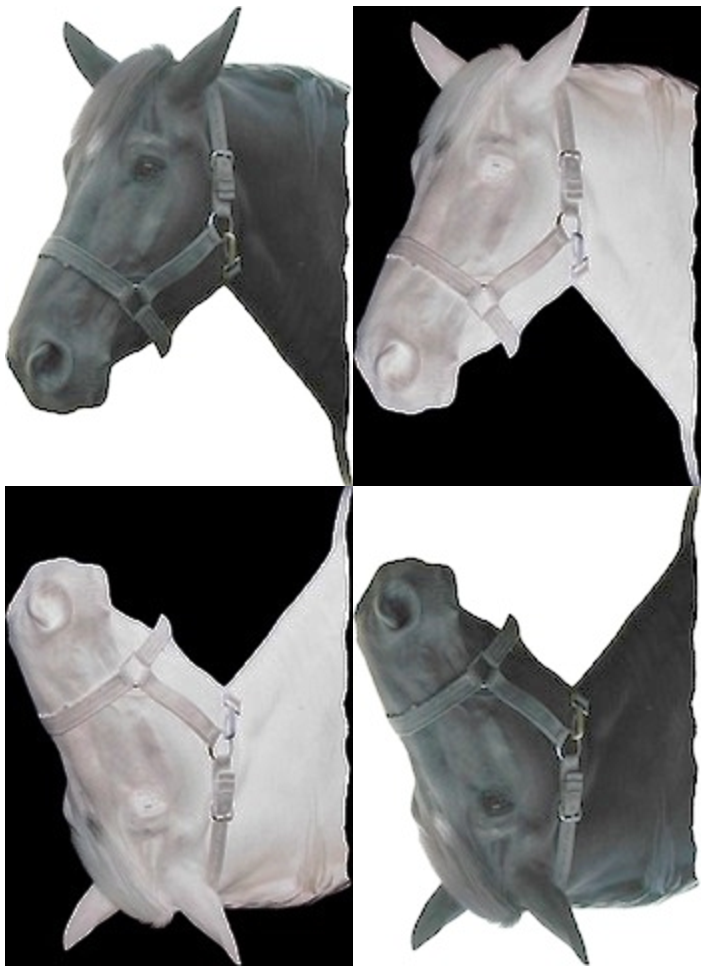
\includegraphics[width=1in]{Pictures/chessReflect.pdf}
\end{center}
\end{exercises}

\section{Errors and error messages}\label{errors}
\index{errors|(}

No system can guarantee that what you type is sensible, and GHCi is no
exception. If something is
wrong, either in an expression to be evaluated or in a script,
you will receive an \textbf{error message}\index{errors!error message}. Try typing
\begin{alltt}
2+(3+4
\end{alltt}
to the GHCi prompt. The error here is\index{errors!syntax}\index{syntax error}
in the \textbf{syntax}\index{syntax}, and is like a sentence in English
which does not have the correct grammatical structure, such as `Fishcake our
camel'. 

The expression
has too few parentheses: after the `\texttt{4}', a closing parenthesis is expected, to match with the
opening parenthesis before `\texttt{3}'. The error message says that something is wrong, but in fact it's not to do with indentation, but rather the lack of a closing parenthesis:
\begin{alltt}
<interactive>:1:7: error: [GHC-58481]
    parse error (possibly incorrect indentation or mismatched brackets)\end{alltt}
In a similar way typing \texttt{2+(3+4))} results in the message
\begin{alltt}
<interactive>:2:8: error: [GHC-58481] parse error on input ‘)’
\end{alltt}
which this time says that (one of) the closing parentheses causes a problem. Now try typing the following expression. 
\begin{alltt}
double square
\end{alltt}
This gives a \textbf{type} error, since \texttt{double} is applied to the
function \texttt{square}, rather than an integer:
\index{type error}\index{errors!type}
\begin{alltt}
<interactive>:5:1: error: [GHC-39999]
    • No instance for ‘Show (Integer -> Integer)’
        arising from a use of ‘print’
        (maybe you haven't applied a function to enough arguments?)
    • In a stmt of an interactive GHCi command: print it\end{alltt}
The message indicates that the system is trying to print something of type 
\texttt{Integer -> Integer}, that is a \emph{function} from integers to integers. It's a bit confused, but says that maybe a function has been applied to too few arguments. That's not the case here, but it might point us to the fact that there's an incorrect function application here: \texttt{double} has been applied to a function rather than a number.


When you get an error message like the one above you need to look
at how the \textbf{term},
in this case \texttt{square} of type \texttt{Integer -> Integer}, does not match the
\textbf{context} in 
which it is used: the context is given in the second line (\texttt{double square})
and the type required by the context, \texttt{Integer}, is given in the last line.

Type errors do not always give rise to
such well-structured error messages. Typing
either \texttt{4 double} or \texttt{4 5} will give rise to 
a message like

\begin{alltt}
<interactive>:6:1: error: [GHC-39999]
    • Could not deduce ‘Num a0’
      from the context: (Num a, Num ((a -> a) -> t))
        bound by the inferred type for ‘it’:
                   forall {a} {t}. (Num a, Num ((a -> a) -> t)) => t
        at <interactive>:6:1-8
      The type variable ‘a0’ is ambiguous
      Potentially matching instances:
        instance Num Integer -- Defined in ‘GHC.Num’
        instance Num Double -- Defined in ‘GHC.Float’
        ...plus three others
        ...plus one instance involving out-of-scope types
        (use -fprint-potential-instances to see them all)
    • In the ambiguity check for the inferred type for ‘it’
      To defer the ambiguity check to use sites, enable AllowAmbiguousTypes
      When checking the inferred type
        it :: forall {a} {t}. (Num a, Num ((a -> a) -> t)) => t
\end{alltt}
We will explore the technical details behind these messages in a later
chapter; for now it is sufficient to read these as `Type Error!'. One thing we can focus on, though, is the place that it says the error occurs: suppose that this was inside a larger program, it would still indicate the appearance of \texttt{4 double} as giving rise to the problem. So, \emph{always take note of where an error is said to occur.}

The last kind of error we will see are \textbf{program errors}. Try the
expression
\index{errors!program}\index{program error}

\begin{alltt} 
4 `div` (3*2-6)
\end{alltt}
We cannot divide by zero (what would the result be?) and so we get the message

\begin{alltt}
*** Exception: divide by zero
\end{alltt}
indicating that a division of \texttt{4} by \texttt{0} has occurred.
More details about the error messages produced by GHCi
can
be found in Appendix \ref{hugsErrors}.
\index{errors|)}



\begin{summary}
The main aim of this chapter is practical, to acquaint the reader with the 
GHCi implementation of Haskell. We have seen how to write simple Haskell
programs, to load them into GHCi and then to evaluate expressions which use
the definitions in the module.

Larger Haskell programs are structured into modules, which can be
imported into other modules. Modules support the Haskell library
mechanism and we illustrate modules in the case study of \texttt{Pictures}
introduced in Chapter \ref{intro}.

We concluded the chapter with an overview of the possible syntax, type 
and program errors in expressions or scripts submitted to GHCi. 

The first two chapters have laid down the theoretical and practical
foundations for the rest of the book, which explores the many aspects of
functional programming using Haskell and GHCi.
\end{summary}
%\end{document} 



%\documentclass{book}\usepackage{sjtfonts}\usepackage{includegraphics}\usepackage{alltt}\usepackage{latexsym}
%\begin{document}\input{defs0}%		miradefs.tex 		    June 1994

% opening and closing a quoted Miranda section

\newcommand{\mira}{\noindent\hrulefill\nopagebreak\so}
\newcommand{\arim}{\nopagebreak\st\hrulefill\\}

% backslash in the Miranda environment
% Only feasible approach is to use \verb+\+
% in line!

%\newcommand{\bs}{$\mi\backslash\!\!$}
%\newcommand{\lbs}{\mbox{\verb+\+}}

% ignoring part of the input

\newcommand{\ignore}[1]{}

% a blank line in a Miranda section

\newcommand{\bl}{\mbox{\ }}

% Signalling a diffculty.

\definecolor{light-gray}{gray}{0.95}

\newcommand{\beware}[2]
 {\medskip\noindent\colorbox{light-gray}{\parbox{\textwidth}
 {\mbox{\large\textbf{#1}} \medskip\noindent\\ #2}\medskip\noindent}}

% Subscripting in Miranda text
\newcommand{\subscr}[2]{\mbox{${\mbox{\texttt{#1}}}_{\mbox{\texttt{#2}}}$}}

%\newcommand{\subscr}[2]{\mbox{${\mbox{\mi #1}}_{\mbox{\smtt #2}}$}}
\newcommand{\aone}{\subscr{a}{1}}
\newcommand{\atwo}{\subscr{a}{2}}
\newcommand{\ak}{\subscr{a}{k}}

\newcommand{\aoneone}{\subscr{a}{1,1}}

\newcommand{\eone}{\subscr{e}{1}}
\newcommand{\etwo}{\subscr{e}{2}}
\newcommand{\ei}{\subscr{e}{i}}
\newcommand{\er}{\subscr{e}{r}}

\newcommand{\fone}{\subscr{f}{1}}
\newcommand{\fl}{\subscr{f}{l}}

\newcommand{\gone}{\subscr{g}{1}}
\newcommand{\gtwo}{\subscr{g}{2}}
\newcommand{\gi}{\subscr{g}{i}}
\newcommand{\gr}{\subscr{g}{r}}

\newcommand{\hone}{\subscr{h}{1}}
\newcommand{\hl}{\subscr{h}{l}}

\newcommand{\pone}{\subscr{p}{1}}
\newcommand{\ptwo}{\subscr{p}{2}}
\newcommand{\pk}{\subscr{p}{k}}

\newcommand{\qone}{\subscr{q}{1}}
\newcommand{\qtwo}{\subscr{q}{2}}
\newcommand{\qk}{\subscr{q}{k}}

\newcommand{\rone}{\subscr{r}{1}}
\newcommand{\rtwo}{\subscr{r}{2}}

\newcommand{\tone}{\subscr{t}{1}}
\newcommand{\ttwo}{\subscr{t}{2}}
\newcommand{\tn}{\subscr{t}{n}}

\newcommand{\vone}{\subscr{v}{1}}
\newcommand{\vtwo}{\subscr{v}{2}}
\newcommand{\vn}{\subscr{v}{n}}

% for regular expressions

\newcommand{\stone}{\subscr{st}{1}}
\newcommand{\sttwo}{\subscr{st}{2}}
\newcommand{\stn}{\subscr{st}{n}}
\newcommand{\rthree}{\subscr{r}{3}}

\newcommand{\eps}{$\varepsilon$}
\newcommand{\trans}[1]{\stackrel{\mbox{\tt #1}}{\longrightarrow}}



% superscript in Miranda text

\newcommand{\superscr}[2]{\mbox{${\mbox{\mi #1}}^{\mbox{\smtt #2}}$}}

% Not equals in Miranda text

\newcommand{\noteq}{\makebox[0pt][l]{=}/}
\newcommand{\overslash}{\makebox[0pt][l]{/}}

% Definitions in complexity chapter

\newfont{\oldSym}{cmsy10}
\newcommand{\Th}{\boldmath$\oldSym\Theta$}
\newcommand{\pow}[1]{\^{}#1}
\newcommand{\leqq}{$\leq$}
\newcommand{\geqq}{$\geq$}
\newcommand{\lll}{$\ll$}
\newcommand{\eqq}{$\equiv$}
\newcommand{\ltwo}{\subscr{log}{2}}

% Indexing

\newcommand{\minx}[1]{\index{#1@{\ttfamily{}#1}}}


\chapter{Basic types and definitions}
\chapstart
\label{BasicTypes}

We have now covered the basics of functional programming and have shown how
simple programs are written, modified and run in GHCi. This chapter
covers Haskell's most important \textbf{basic types} and also shows
how to write definitions of functions which have multiple
\textbf{cases} to cover alternative situations. We conclude by looking
at some of the details of  the \textbf{syntax} of Haskell.

Haskell contains a variety of numerical types. We have already seen the 
\texttt{Integer} type in use; we shall cover this as well as the (related) \texttt{Int} type and the \textbf{floating-point}
fractional numbers, \texttt{Float}.

Often in programming we want to make a choice of values, according to
whether or not a particular \textbf{condition} holds. These conditions
include tests of whether one number is greater than another; whether
two values are equal, and so on. The results of these tests -- \texttt{True}\minx{True} if the
condition holds and \texttt{False}\minx{False} if it fails -- are called the
\textbf{Boolean}\index{Boolean} values, after the nineteenth-century logician George
Boole,\index{Boole, George} and they form the Haskell type
\texttt{Bool}\minx{Bool}. In this chapter we cover the Booleans, and how they are used
to give choices in function definitions by means of
\textbf{guards}\index{guard}.

Next, we look at the types of characters and strings. Characters -- 
individual letters, digits, spaces and so forth -- are 
given by the Haskell type \texttt{Char}\minx{Char}. Strings of letters and other characters make up strings, in the Haskell type \texttt{String}\minx{String}.

The chapter provides
reference material for the basic types; a reader may
skip the treatment of \texttt{Float} and much of the detail about
\texttt{Char} and \texttt{String}, referring back to this chapter when necessary.

Each section here contains examples of functions, and the exercises build
on these.
Looking ahead, this chapter gives a foundation on top of which we look
at a variety of different ways that programs can be designed and
written, which
is the topic of the next chapter. 

\section{The Booleans: \texttt{Bool}}
\markright{The Booleans: \texttt{\runinghead Bool}}
\index{Booleans|(}
\minx{Bool}

The Boolean values \texttt{True} and \texttt{False}\minx{True}\minx{False}
represent the results of tests,
which might, for instance, 
compare two numbers for equality, or check
whether the first is smaller than the second. The Boolean type in Haskell is
called \texttt{Bool}.
The Boolean operators provided in the language are:

\begin{center}\minx{\&\&}\minx{"|"|}
\begin{mytable}
\texttt{\&\&} & and  \\
\texttt{||} & or \\
\texttt{not} & not\minx{not}
\end{mytable}
\end{center}

\noindent
Because \texttt{Bool} contains only two values, we can define the meaning of
Boolean operators by \textbf{truth tables}\index{truth table} which show
the result of applying the operator to each possible combination of
arguments. For instance, the third line of the first table says that
the value of \texttt{False \&\& True} is \texttt{False} and that the value of 
\texttt{False || True}
is \texttt{True}.

\medskip
\begin{tabular}{cc|cc}
\tone & \ttwo & \mi \tone\ \&\& \ttwo & \tone \mbox{\texttt{||}} \ttwo \\ \hline
\mi T & \mi T & \mi  T &  \mi T \\
\mi T &  \mi F & \mi  F &  \mi T \\
\mi F &  \mi T & \mi  F &  \mi T \\
\mi F &  \mi F & \mi  F & \mi  F \\
\end{tabular}
\hspace*{1cm}\begin{tabular}[b]{c|c}
\tone & \mi not \tone  \\ \hline
\mi T & \mi F  \\
\mi F &  \mi T  
\end{tabular}

\subsection*{Defining Boolean functions}

Booleans can be the arguments to or the results of functions. We look at some
examples now. 


The
`built-in or', \texttt{||}, is called `inclusive'
\index{inclusive or} because it returns \texttt{True} if either one or both of its
arguments are \texttt{True}. `Exclusive or' \index{exclusive or}
is the function which returns \texttt{True} when \emph{exactly} one but not both of its
arguments has the value
\texttt{True}; it is like the
`or' of a restaurant menu: you may choose vegetarian moussaka or 
fish as your main course,
but not both!
The definition here mirrors the definition: the result is true if either \texttt{x} or \texttt{y} is true (\texttt{x || y}), and they are not both true (\texttt{not (x \&\& y)}):
\medskip
\begin{alltt}\minx{exOr}
exOr :: Bool -> Bool -> Bool
exOr x y = (x || y) \&\& not (x \&\& y)
\end{alltt}

 

We can picture the function definition using boxes for functions, and
lines for values, as we saw in Chapter \ref{intro}. Lines coming into a
function box represent the arguments, and the line going out the result.
\begin{center}\index{function!box diagram}
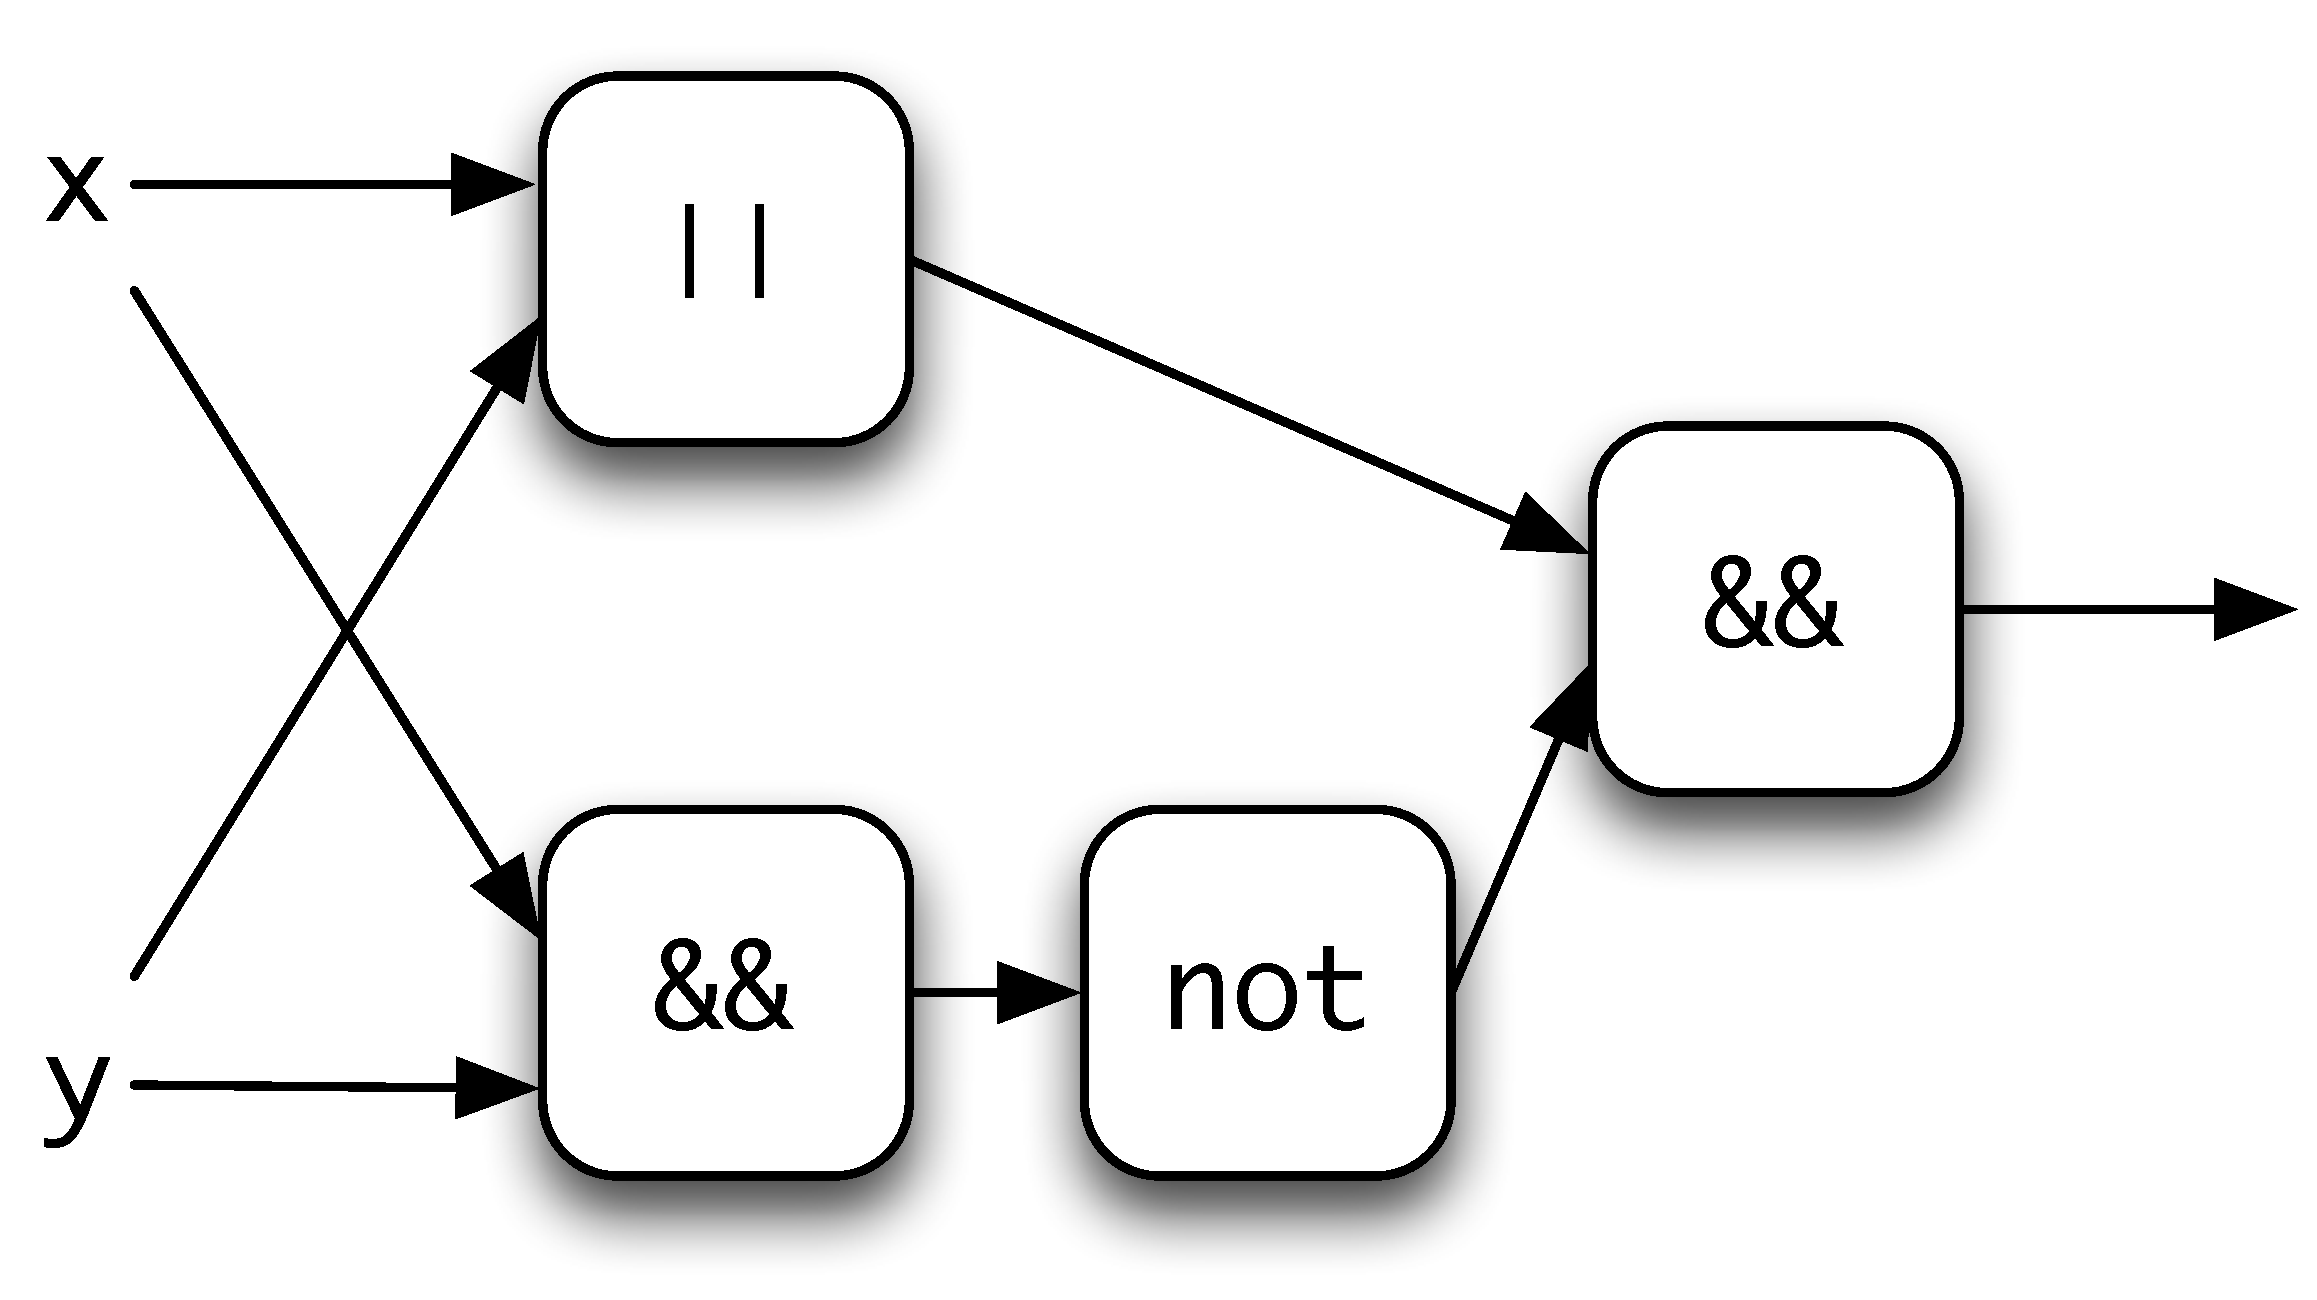
\includegraphics[height=4cm]{Pictures/exOr.pdf}
\end{center} 
Boolean values can also be compared for equality and inequality using
the operators
\texttt{==}\minx{==} and \texttt{/=}\minx{/=}, which both have the type
\begin{alltt}
Bool -> Bool -> Bool
\end{alltt}
Note that \texttt{/=} is the same function as \texttt{exOr}, since both
return the result \texttt{True} when exactly one of their arguments is
\texttt{True}.

\subsection*{Literals and definitions}

Expressions like \texttt{True} and \texttt{False}, and also numbers like
\texttt{2}, are known as
\textbf{literals}.\index{literal}\index{value!literal}
These are values which are given literally, and which need no
evaluation; the result of evaluating a literal is the literal itself.

We can use the literals \texttt{True} and \texttt{False} as arguments, in defining
\texttt{not} for ourselves:
\begin{alltt}\minx{myNot}
myNot :: Bool -> Bool
myNot True  = False
myNot False = True
\end{alltt}
We can also use a combination of literals and variables on the left-hand side of
equations defining \texttt{exOr}:
\begin{alltt}
exOr True  x = not x
exOr False x = x
\end{alltt}
Here we see a definition of a function which uses two equations: the
first applies whenever the first argument to \texttt{exOr} is
\texttt{True} and the second when that argument is \texttt{False}.

Definitions which use \texttt{True} and \texttt{False} on the left-hand
side of equations are often more readable than definitions which only
have variables on the left-hand side. This is a simple example of the
general \textbf{pattern matching}\index{pattern matching} 
mechanism in Haskell, which we look at
in detail in Chapter \ref{tupleList}.


\subsection*{Testing}

We can write some QuickCheck properties to test our new implementation of \texttt{not} and our multiple implementations of exclusive or. We test \texttt{myNot} against the built in function, and test our exclusive or functions -- let's call them \texttt{exOr} and \texttt{exOr1}:
\begin{alltt}\minx{prop\_myNot}
prop_myNot :: Bool -> Bool

prop_myNot x =
    not x == myNot x

prop_exOrs :: Bool -> Bool -> Bool

prop_exOrs x y =
    exOr x y == exOr1 x y 
\end{alltt}\minx{prop\_exOrs}
and running them gives the results that we expect:
\begin{alltt}
\textsl{*Chapter3>} quickCheck prop_myNot
\textsl{+++ OK, passed 100 tests.}
\textsl{*Chapter3>} quickCheck prop_exOrs
\textsl{+++ OK, passed 100 tests.}
\end{alltt}
We can also check the earlier assertion that \texttt{exOr} and \texttt{/=} have the same behaviour over Booleans with this property:
\begin{alltt}
prop_exOr2 :: Bool -> Bool -> Bool

prop_exOr2 x y =
    exOr x y == (x /= y)
\end{alltt}


\begin{exercises}
\item
Give another version of the definition of `exclusive or' which
works informally
like this: `exclusive or of \texttt{x} and \texttt{y} will be \texttt{True} if either
\texttt{x} is \texttt{True} and \texttt{y} is \texttt{False}, or \texttt{x} is \texttt{False} and \texttt{y} is \texttt{True}'.

\item Give the `box and line' diagram corresponding to your answer to the 
previous question.

\item Using literals on the left-hand side we can make the truth table
for a function into its Haskell definition. Complete the following
definition of \texttt{exOr} in this style.
\begin{alltt}
exOr True True  = ...
exOr True False = ...
  ...
\end{alltt}

\item Give your own definitions of the built-in \texttt{\&\&} and \texttt{||}. If you want to use the same operator for \texttt{\&\&}, say, you will need to make sure you hide its import. You can do this by adding it to the list of what is hidden, thus:
\begin{alltt}
import Prelude hiding (max,(&&))
\end{alltt}
after the \texttt{module} declaration at the start of the \texttt{Chapter3} module.

\item Give two different definitions of the \texttt{nAnd} function 
\begin{alltt}
nAnd :: Bool -> Bool -> Bool
\end{alltt}
which returns the result \texttt{True} except when both its arguments
are \texttt{True}. Give a diagram illustrating one of your definitions.

\item
Give line-by-line calculations of 
\begin{alltt}
nAnd True True
nAnd True False
\end{alltt}
for each of your definitions of \texttt{nAnd} in the previous exercise.


\item
Write QuickCheck properties to test the functions you have written in the earlier exercises. You might be able to check one version of a function against another, or perhaps think up different properties for your functions.

\index{Booleans|)}
\end{exercises}


\section{The integers: \texttt{Integer} and \texttt{Int}}
\markright{The integers: \texttt{\runinghead Integer}}
\label{ints}
\index{numbers!integers|(}\minx{Integer}

The Haskell type \texttt{Integer} contains the integers, which are the whole numbers, positive, zero and negative, used for counting; they
are written like this:

\begin{alltt}
0
45
-3452
2147483647
\end{alltt} 
Integers in the \texttt{Integer} type can be as large as you wish: looking back at the GHCi screenshots in Figures \ref{GHCiSessionMac} and \ref{WinGHCiSession} you can see examples of this. We do arithmetic on integers using the following operators and functions.

\medskip
\noindent
\begin{mytable}
\texttt{+}\minx{+} & The sum of two integers. \\
\texttt{*}\minx{*} & The product of two integers.\\
\texttt{\^{}}\minx{\^{}} & Raise to the power; \texttt{2\^{}3} is \texttt{8}.\\
\texttt{-}\minx{-} & The difference of two integers, when infix: \texttt{a-b}; 
the integer of opposite sign, when prefix: \texttt{-a}.\\ 
\texttt{div}\minx{div} & Whole number division; for example \texttt{div 14 3} is \texttt{4}. This
can also be written \texttt{14 `div` 3}.\\
\texttt{mod}\minx{mod} & The remainder from whole number division; for example \texttt{mod 14 3}
(or \texttt{14 `mod`
3}) is \texttt{2}.\\
\texttt{abs\minx{abs}} & The absolute value of an integer; remove the sign.\\
\texttt{negate\minx{negate}} & The function to change the sign of an integer.\\
\end{mytable}


\medskip
\noindent
Note that \texttt{`mod`} surrounded by \textbf{backquotes}
\index{backquote (\texttt{`})} is written between its two arguments, is
an {\bf infix}\index{function!infix version of}\index{infix version of a function} 
version of the function \texttt{mod}.
Any function can be made infix in this
way. 

In what follows we will use the term the \textbf{natural numbers} for the
\index{numbers!natural numbers}
non-negative integers: \texttt{0}, \texttt{1}, \texttt{2}, \ldots.

\begin{figure}[t]
\index{pitfalls!negative literals}\index{literal!negative}
\beware{Negative literals}{Negative literals cause problems in Haskell, because of the way that they have been defined. For example the number minus twelve is written as \texttt{-12}, but the prefix `\texttt{-}'
can often get confused with the infix operator to subtract one number from another
and can lead to unforeseen and confusing type error messages. For
example, the application
\begin{alltt}
negate -34
\end{alltt}
\noindent is interpreted as `negate minus \texttt{34}' and
leads to a GHCi error message: we discuss how to interpret that in the next note.

\medskip
\noindent
If you are in any doubt about the source of an error and you are
dealing with negative numbers you should
enclose them in parentheses, thus: \texttt{negate (-34)}; it will do no harm! See
Section \ref{operators} for more details.}
\end{figure}

\begin{figure}[t]
\beware{Understanding GHCi error messages}{When you first see an error message like this
\begin{alltt}\index{GHCi!understanding error messages}
    No instance for (Num (a -> a))
      arising from a use of `-' at <interactive>:1:0-9
    Possible fix: add an instance declaration for (Num (a -> a))
      In the expression: negate - 34
    In the definition of `it': it = negate - 34
\end{alltt}
you could be forgiven for being bemused, because it talks about things we've not covered yet. 

\medskip\noindent
Don't despair! What you can do is \textbf{extract some useful information} from it, particularly from the parts highlighted with a white background. The first one says that there's something wrong with a use of `\texttt{-}' on the line typed \emph{interactively}; the second one says it's because of the expression \texttt{negate - 34}, where you can see that the system has mis-interpreted your use of \texttt{-34}.

\medskip\noindent
So, you need to be a detective, pulling out all the \emph{clues} that you can find. These will usually be some indication of \emph{where the error occurs} and \emph{the reason for it}. If nothing else, it should give you a clue of where to look.
}
\end{figure}





\subsection*{Relational operators}

There are ordering and (in)equality\index{order}\index{equality}
relations over the integers, as there are
over all basic types. These functions
take two integers as input and return a \texttt{Bool}, that is 
either \texttt{True} or \texttt{False}. The relations are 
 
\medskip
\noindent
\begin{mytable}
\mi > & greater than (and not equal to) \minx{>}\\
\mi >= & greater than or equal to \minx{>=}\\
\mi == & equal to\minx{==} \\
\mi /= & not equal to\minx{/=}\\
\mi <= & less than or equal to\minx{<=}\\
\mi < & less than (and not equal to)\minx{<}
\end{mytable}


\medskip
\noindent
A simple example using these definitions is a function to test whether
three \texttt{Integer}s are equal.
\begin{alltt}\minx{threeEqual}
threeEqual :: Integer -> Integer -> Integer -> Bool
threeEqual m n p = (m==n) \&\& (n==p)
\end{alltt}
%\vspace{-5pt}


\begin{figure}[t]
\beware{Fixed-size integers: the \texttt{Int} type}{\minx{Int}
The \texttt{Int} type represents integers in a fixed amount of space, and
so can only represent a finite range of integers. The value
\texttt{maxBound} gives the greatest value in the type, which happens to be
\texttt{2147483647}. 

\medskip
\noindent
For many integer
calculations these fixed size numbers are suitable, and they have the advantage of being more efficient, but if larger
numbers may be 
required it's better to use the \texttt{Integer}\minx{Integer} type, which can accurately represent whole numbers of
any size. 

\medskip
\noindent
The reason that we introduce \texttt{Int} at all is that because some of the standard Haskell functions
which we introduce later in the chapter use the \texttt{Int} type, rather than \texttt{Integer}.

\medskip
\noindent
What functions and operators can we use over \texttt{Int}? All the functions we have already given for \texttt{Integer}, in fact, because these functions are \emph{overloaded}: we look at this in Section \ref{overlIntro}. We can also covert between the two types using
\begin{alltt}\minx{fromInteger}\index{toInteger}
fromInteger :: Integer -> Int
toInteger   :: Int -> Integer
\end{alltt}}
\end{figure}


\begin{exercises}
\vspace{-3pt}
\item
Explain the effect of the function defined here:
\begin{alltt}
mystery :: Integer -> Integer -> Integer -> Bool
mystery m n p = not ((m==n) \&\& (n==p))
\end{alltt}
Hint: if you find it difficult to answer this question directly, try to
see what the function does on some example inputs.

\item
Define a function 
\begin{alltt}
threeDifferent :: Integer -> Integer -> Integer -> Bool
\end{alltt}
so that the result of \texttt{threeDifferent m n p} is \texttt{True}
only if all three of the numbers \texttt{m}, \texttt{n} and \texttt{p}
are different.

What is your answer for \texttt{threeDifferent 3 4 3}? Explain why you
get the answer that you do.

\item
This question is about the function
\begin{alltt}
fourEqual :: Integer -> Integer -> Integer -> Integer -> Bool
\end{alltt}
which returns the value \texttt{True} only if all four of its arguments
are equal.

Give a definition of \texttt{fourEqual} modelled on the
definition of \texttt{threeEqual} above. Now give a definition of
\texttt{fourEqual} which {\em uses\/} the function \texttt{threeEqual}
in its definition. Compare your two answers.

\item
Give line-by-line calculations of
\begin{alltt}
threeEqual (2+3) 5 (11 `div` 2)
mystery (2+4) 5 (11 `div` 2)
threeDifferent (2+4) 5 (11 `div` 2)
fourEqual (2+3) 5 (11 `div` 2) (21 `mod` 11)
\end{alltt}

\item
Devise QuickCheck tests for the functions that you have defined here.



\index{numbers!integers|)}%
\end{exercises}
\vspace{-20pt}

\section{Overloading}
\label{overlIntro}
\index{overloading}%
\index{name!overloading of}%

\texttt{Integer}s, \texttt{Int}s and Booleans can all compared for equality, and the same
symbol \texttt{==} is used for all these operations, even though they
are different. Indeed, \texttt{==} will be used for equality over
any type \texttt{t} for which we are able to define an equality
operator. This means that \texttt{(==)} will have the type 
\begin{alltt}\minx{==}
Int -> Int -> Bool
Integer -> Integer  -> Bool
Bool -> Bool -> Bool
\end{alltt}
and indeed \texttt{t -> t -> Bool} if the type \texttt{t}
carries an equality.

Using the same symbol or name for different operations is called
\textbf{overloading}. A number of symbols in Haskell are overloaded, and
we will see in Chapter \ref{typeClasses} how overloading is handled in the
type system of Haskell, and also how users can define their own
overloaded operators or names.

\beware{The type for equality}{The type for equality, \texttt{t -> t -> Bool} for any type \texttt{t} carrying an equality, \emph{doesn't} allow us to compare elements from different types for equality. So, if we evaluate\index{equality!type of}
\begin{alltt}
2 == True
\end{alltt}
we get an error message from GHCi. Of course, there's not much point in comparing values of different types, because they will never be equal! We'll come back to this in Chapter \ref{typeClasses}.
}

\section{Guards}
\label{guards}
\index{guard|(}
\index{Boolean!guard|see{guard}}

Here we explore how conditions or \textbf{guards} are used to give
alternatives in the definitions of functions. A guard is a Boolean expression, and
these expressions are used to express various cases in the definition of a function.
 
We take as a running
example in this section
functions which compare integers for size, and start by looking
at the example of the function to return the maximum value of two
integers. When the two numbers are the same then we call their common value
the maximum.
\begin{alltt}\minx{max}
max :: Integer -> Integer -> Integer
max x y
  | x >= y      = x
  | otherwise   = y
\end{alltt}
How do we read a definition like this, which appears in the Haskell prelude? 
%\psdraft
\begin{center}
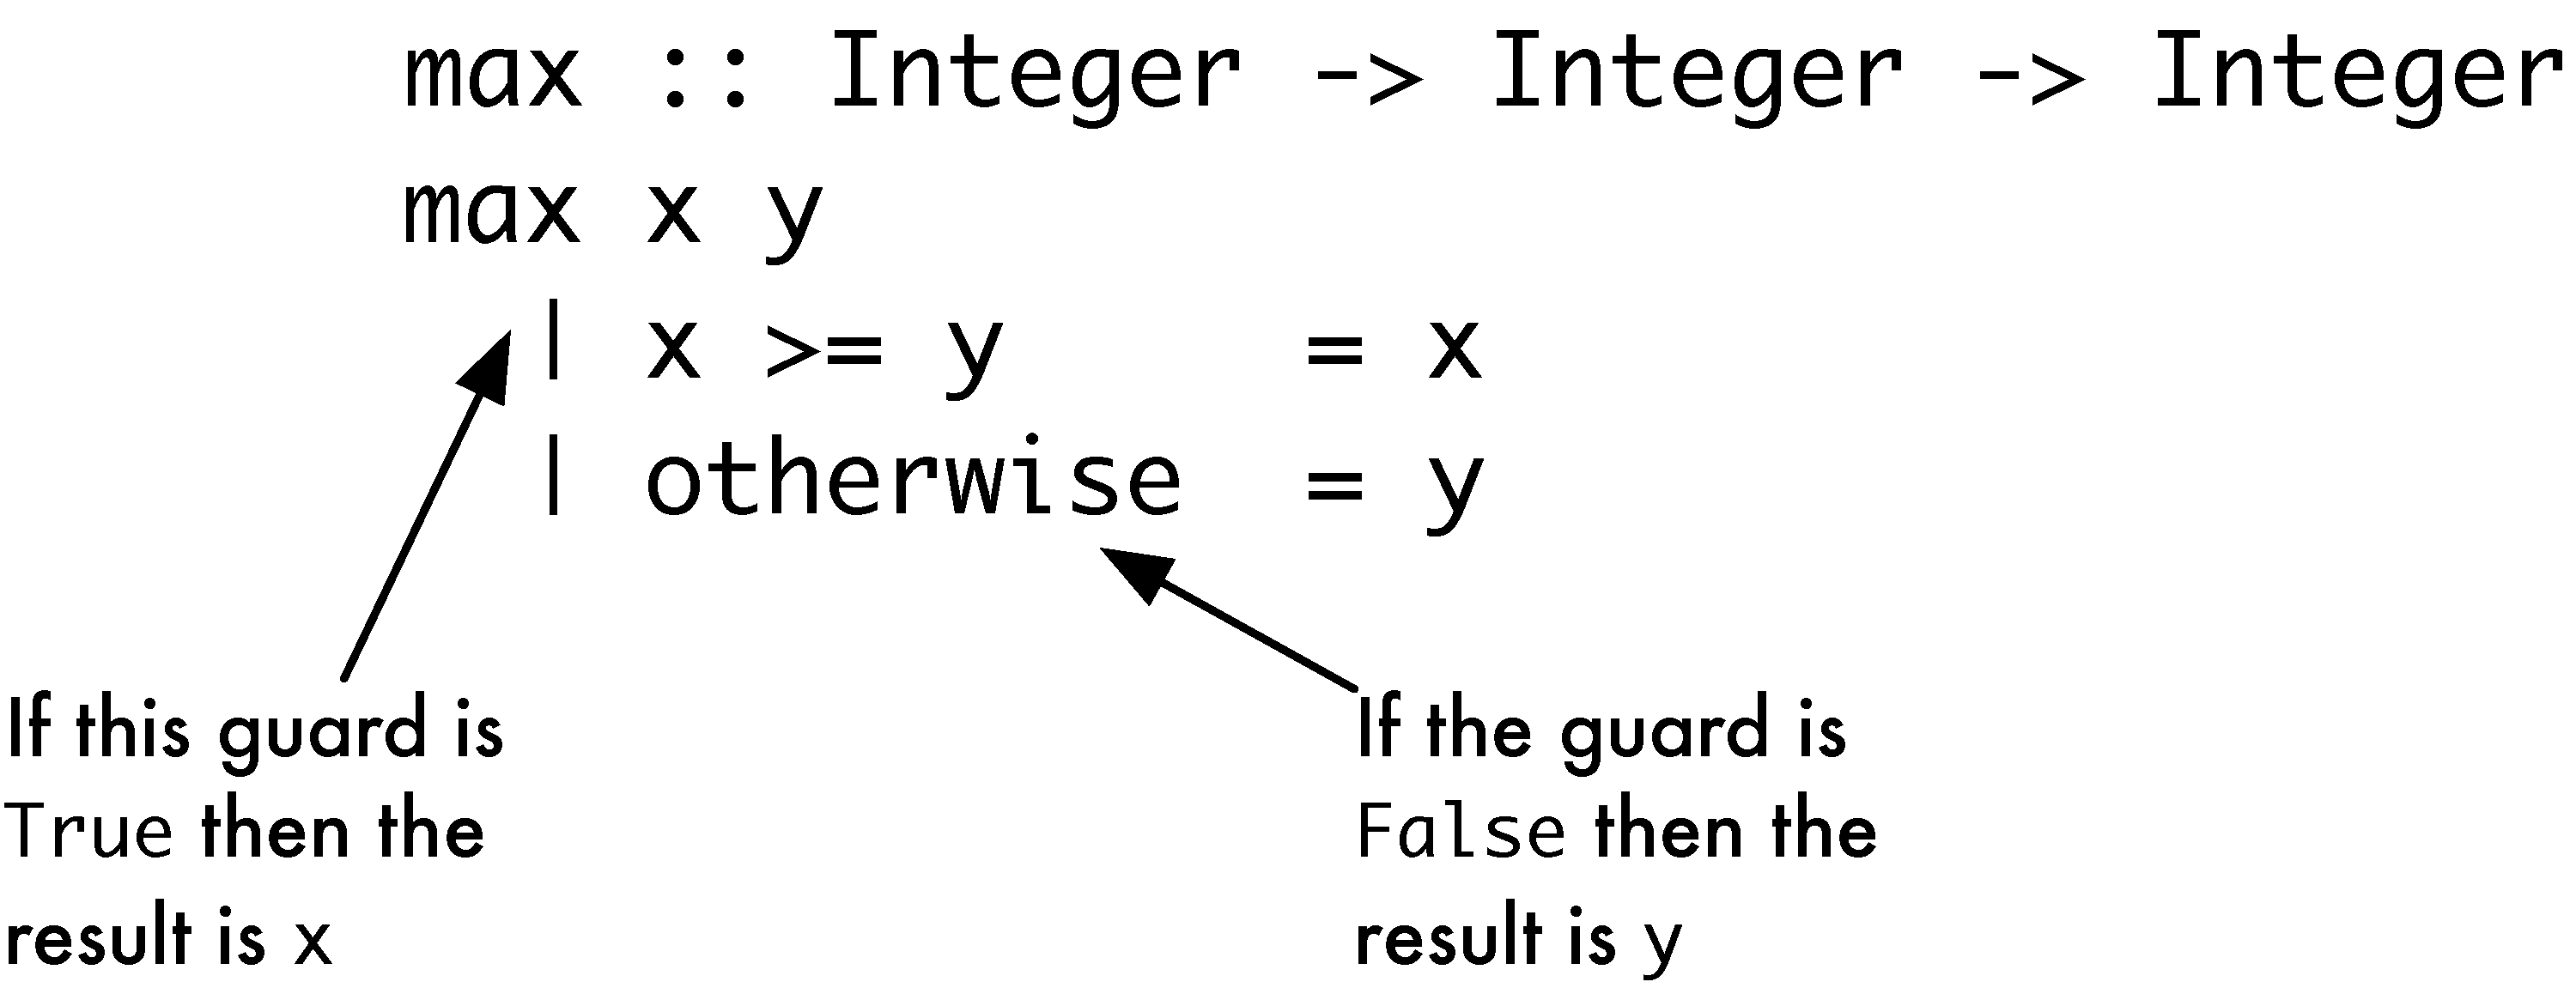
\includegraphics[width=4in]{Pictures/max.pdf}
\end{center} 
%\psfull
In general, if the first guard (here \texttt{x>=y})
is \texttt{True} then the corresponding value is the result (\texttt{x} in this case).
On the other hand, if the first guard is \texttt{False}, then we look at the second, and so on. 
An \texttt{otherwise}\minx{otherwise}
guard will hold whatever the arguments, so that in the case of \texttt{max} the result is \texttt{x} if 
\texttt{x>=y} and \texttt{y} otherwise, that is in the case that \texttt{y>x}.

 
An example in which there are multiple guards is a definition of the
maximum of three inputs.
\begin{alltt}\minx{maxThree}
maxThree :: Integer -> Integer -> Integer -> Integer
maxThree x y z
  | x >= y \&\& x >= z    = x
  | y >= z              = y
  | otherwise           = z
\end{alltt}
How does this definition work? The first guard
\begin{alltt}
x >= y \&\& x >= z
\end{alltt}
tests whether \texttt{x} is the maximum of the three inputs; if it is \texttt{True}
the corresponding result is \texttt{x}. If the guard fails, then \texttt{x} is
not the maximum, so there has to be a choice between \texttt{y} and \texttt{z}. The
second guard is therefore
\begin{alltt}
y >= z
\end{alltt}
If this holds, the result is \texttt{y}; otherwise the result is
\texttt{z}. We will go back to the example of \texttt{maxThree} in Section
\ref{probSolvIntro}.

We first gave a general form for simple function definitions in Chapter
\ref{intro}; we can now strengthen this to give a general form for
function definitions with guards in Figure \ref{funGuardDef}. Note that
the \texttt{otherwise} is not compulsory.
\index{function definition!general form}

%fig3.1
\begin{figure}
\begin{center}
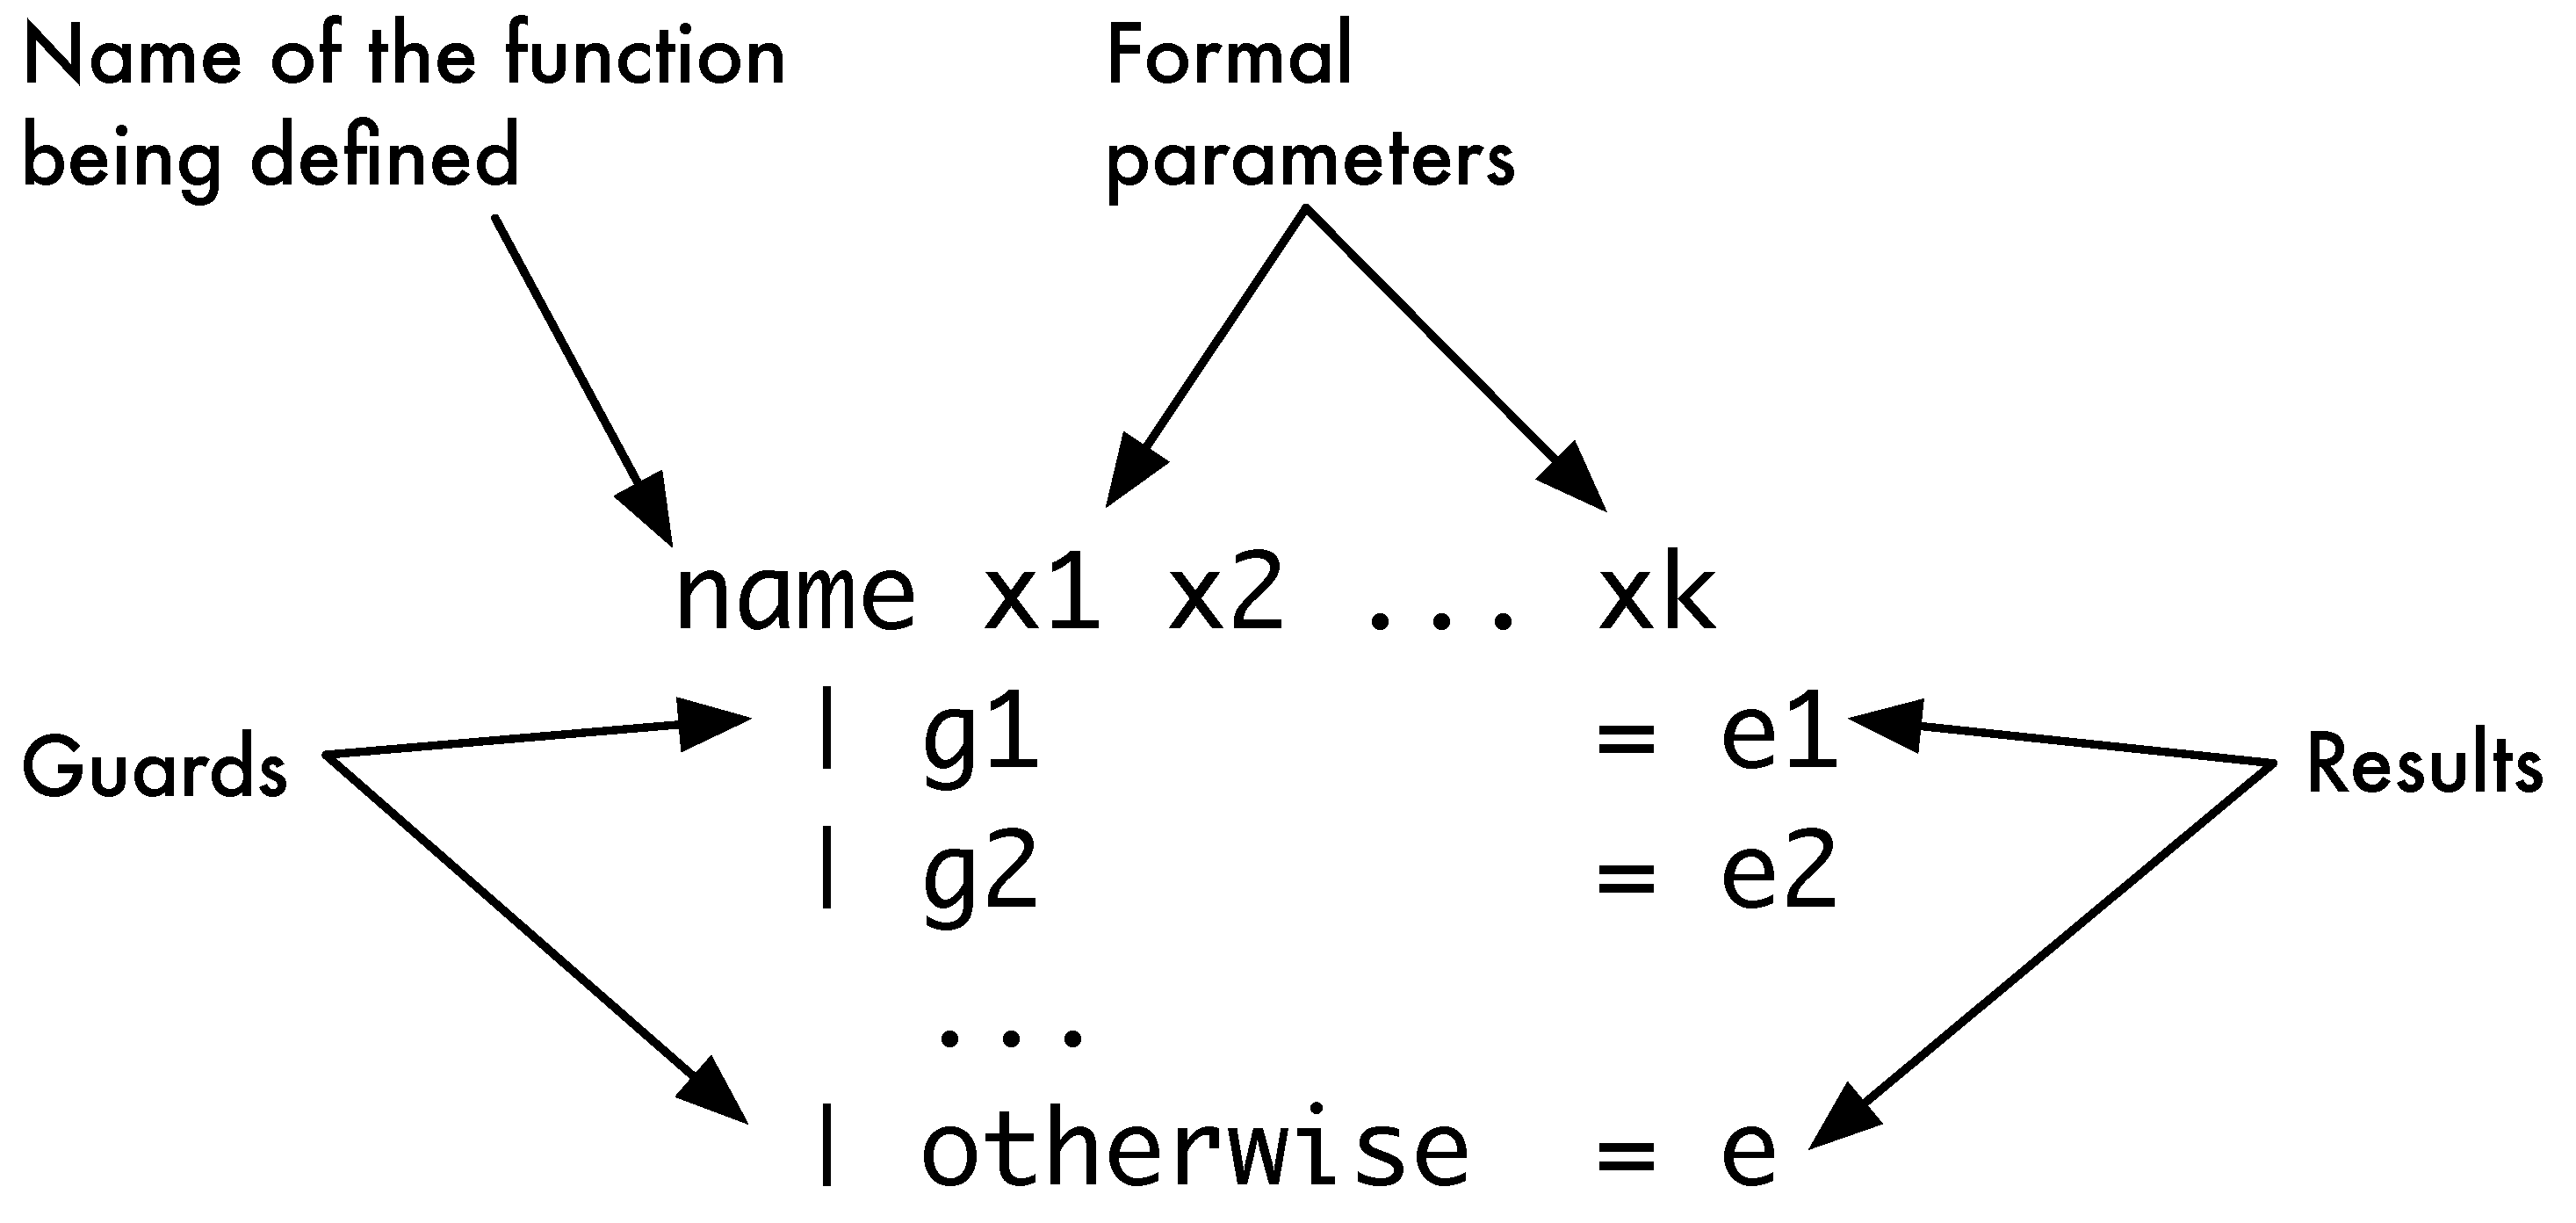
\includegraphics[width=4in]{Pictures/funGuardDef.pdf}
\end{center} 
\caption{The general form for function definitions with guards.}
\label{funGuardDef}
\end{figure}

We also saw in Chapter \ref{intro} that we can write down line-by-line
\textbf{calculations}\index{calculation!guards}
of the values of expressions. How do guards fit into this model? When we
apply a function to its arguments we need to know which of the cases
applies, and to do this we need to evaluate the guards until we find a
guard whose value is \texttt{True}; once we find this, we can evaluate
the corresponding result. Taking the example of \texttt{maxThree}, we
give two examples in which we perform the evaluation of guards on lines
beginning `\texttt{??}'.
\begin{alltt}
maxThree 4 3 2
  ?? 4>=3 \&\& 4>=2
  ?? \step{}True \&\& True
  ?? \step{}True
\step{}4
\end{alltt}
In this example the first guard we try, \texttt{4>=3 \&\& 4>=2},
gives \texttt{True} and so the result is the corresponding value,
\texttt{4}.
In the second example we have to evaluate more than one guard.
\begin{alltt}
maxThree 6 (4+3) 5
  ?? 6>=(4+3) \&\& 6>=5
  ?? \step{}6>=7 \&\& 6>=5
  ?? \step{}False \&\& True
  ?? \step{}False
  ?? 7>=5
  ?? \step{}True
\step{}7
\end{alltt}
In this example we first evaluate the first guard, \texttt{6>=(4+3) \&\&
6>=5}, which results in \texttt{False}; we therefore evaluate the
second guard, \texttt{7>=5}, which gives \texttt{True}, and so the
result is \texttt{7}. 

Once we have calculated the value of the second
argument, \texttt{(4+3)}, we do not re-calculate its value when we
look at it again. This is not just a trick on our part; the GHCi system will only 
evaluate an argument like \texttt{(4+3)} 
once, keeping its value in case it is needed again, as indeed it is in
this calculation. This is one aspect of lazy evaluation, which is the
topic of Chapter \ref{lazy}.

\subsection*{Conditional expressions}
\index{conditional expression}\index{expression!conditional}
\index{Boolean!conditional expression}
\index{if@{\texttt{if}\ldots\texttt{then}\ldots\texttt{else}}}

Guards are conditions which distinguish between
different cases in definitions\break of functions. We
can also write general conditional expressions by means of
the\break{\texttt{if}\ldots\texttt{then}\ldots\texttt{else}} construct of Haskell. The value of
\begin{alltt}
if condition then m else n
\end{alltt}
is \texttt{m} if the \texttt{condition} is \texttt{True} and is
\texttt{n} if the \texttt{condition} is \texttt{False}, so that the
expression \texttt{if False then 3 else 4}
has the value \texttt{4}, and in general
\begin{alltt}
if x >= y then x else y
\end{alltt}
will be the maximum of \texttt{x}
and \texttt{y}. This shows that we can write \texttt{max'} in a
different way thus:
\begin{alltt}
max' :: Integer -> Integer -> Integer
max' x yMax
  = if x >= y then x else y
\end{alltt}
We tend to use the guard form rather than this, but we will see examples
below where the use of \texttt{if ...\ then ...\ else ...{}} is more
natural.

\subsection*{Testing}

We can test our implementations of `maximum' by checking that they have the same behaviour, as we did earlier, writing a QuickCheck property like this:
\begin{alltt}\minx{prop\_compareMax}
prop_compareMax :: Integer -> Integer -> Bool
prop_compareMax x y =
    max x y == max' x y
\end{alltt}
But this is not the only way of writing properties. We can often write down a collection of properties which together say what a function should do. In the case of \texttt{max} we can say two things
\begin{itemize}
\item
The maximum of \texttt{x} and \texttt{y} will be greater than or equal to both \texttt{x} and \texttt{y}.
\item
The maximum of \texttt{x} and \texttt{y} will actually be equal to one (or both) of  \texttt{x} and \texttt{y}.
\end{itemize}  
We can write these two as QuickCheck properties, 
\begin{alltt}
prop_max1, prop_max2 :: Integer -> Integer -> Bool

prop_max1 x y =
    x <= max x y && y <= max x y

prop_max2 x y =
    x == max x y || y == max x y
\end{alltt}
and check whether they hold. 

\begin{figure}[t]
\beware{Properties can be wrong too}{\index{property!incorrect}
Sometimes we make mistakes writing properties. Suppose we'd written the property 
\texttt{prop\_max2} like this instead:
\begin{alltt}
prop\_max3 x y =

\ \ \ \ (x == max x y) `exOr` (y == max x y)
\end{alltt}
recall that QuickCheck will give us a \emph{counterexample}, that is, an example of where the test fails:   
\begin{alltt}
\textsl{*Chapter3>} quickCheck prop\_max3

\textsl{*** Failed! Falsifiable (after 1 test):} 
 
\textsl{0}

\textsl{0}
\end{alltt}
The example shows that the property fails when the two arguments are the same. 
That's the fault of the property, as we'd forgotten about this particular case. 
So, \textbf{when a property fails, we need to look both at the functions it is meant to test, 
and at the property itself}.}
\end{figure}


\begin{figure}[t]
\beware{Redefining prelude functions}{\label{redefName}%
The \texttt{max} function is defined in the prelude,
\texttt{Prelude.hs},\index{prelude, redefining functions in}
\index{function definition!redefining prelude functions}
and if a definition 
\begin{alltt}
max :: Integer -> Integer -> Integer
\end{alltt}
\noindent appears in a script then this definition will conflict with
the prelude definition, leading to a GHCi error messages like this
\begin{alltt}
\ \ \ \ Ambiguous occurrence `max'

\ \ \ \ It could refer to either `Chapter3.max', defined at ...

\ \ \ \ \ \ \ \ \ \ \ \ \ \ \ \ \ \ \ \ \ \ or `Prelude.max', imported from Prelude ...
\end{alltt}
\noindent To redefine the prelude functions \texttt{max} and \texttt{min}, say, the line
\begin{alltt}
import Prelude hiding (max,min)\minx{import}\minx{hiding}
\end{alltt}
\noindent which overrides the usual import of the prelude should be included at
the top of the module, after its \texttt{module}
statement.

Many of the functions defined in this text are in fact included in the
prelude, and so this technique needs to be used whenever you want to 
redefine one of these.
}\end{figure}

\begin{exercises}
\item
Give calculations of 
\begin{alltt}
max (3-2) (3*8)
maxThree (4+5) (2*6) (100 `div` 7)
\end{alltt}

\item
Give definitions of the functions
\begin{alltt}
min      :: Int -> Int -> Int
minThree :: Int -> Int -> Int -> Int
\end{alltt}
which calculate the minimum of two and three integers, respectively.

\item
Define QuickCheck properties to test the functions \texttt{maxThree}, \texttt{min} and \texttt{minThree}.


\index{guard|)}
\end{exercises}
\section{Characters and strings}
\markright{The characters: \texttt{\runinghead Char}}
\label{char}
\index{characters|(}
\minx{Char}
People and computers communicate using keyboard input and screen output,
which are based on sequences of {\bf characters}, that is letters, digits
and `special' characters like space, tab, newline and end-of-file. Haskell
\index{characters!tab}
\index{characters!end-of-file}
contains a built-in type of characters, called \texttt{Char}.\minx{Char} Sequences  or \textbf{strings} of characters form the Haskell \texttt{String} type. 

\subsection*{Characters: \texttt{Char}}

Literal characters\index{characters!literal} 
are written inside single quotes, thus {\mi 'd'} is
the Haskell representative of the character d. Similarly {\mi '3'}
is the character three. Some special characters are represented as 
follows

\medskip
\noindent
\begin{mytable}
tab & \texttt{'\bs{t}'}\\[3pt]\index{tab (\texttt{\bs{}t})}  
newline & \texttt{'\bs{n}'}\\[3pt]\index{newline (\texttt{\bs{}n})}
backslash (\verb+\+) & \texttt{'\bs{\symbol{92}}'}\\[3pt]\index{backslash (\texttt{\bs{}\bs{}})}
single quote (\texttt{'}) & \texttt{'\bs{'}'}\\[3pt]\index{single quote (\texttt{\bs{}'})}
double quote (\texttt{"}) & \texttt{'\bs{"}'}\\[3pt]\index{double quote (\texttt{\bs{\symbol{34}}})}
\end{mytable} 

\medskip
\noindent
There is a standard coding for characters as integers, called the ASCII
\index{characters!ASCII coding}
coding. The capital letters \texttt{'A'} to \texttt{'Z'} have the sequence of
codes from \texttt{65} to \texttt{90}, and the small letters \texttt{'a'} to 
\texttt{'z'} the codes \texttt{97} to \texttt{122}. The character with code \texttt{34}, for
example, can be written \texttt{'\bs{34}'}, and \texttt{'9'} and \texttt{'\bs{57}'} have the same
meaning. ASCII has recently been extended to
the Unicode\index{characters!Unicode}\index{Unicode} standard, which contains characters from other character sets
than English.

There are conversion functions between characters and their numerical
codes
which convert an integer into a character, and vice versa. 
\vspace{2pt}

\begin{alltt}
fromEnum :: Char -> Int\minx{fromEnum}
toEnum :: Int -> Char\minx{toEnum}
\end{alltt} 
\vspace{2pt}

\noindent The coding functions can be used in defining functions over
\texttt{Char}. To convert a small letter to a capital an offset needs to be
added to its code:
\vspace{2pt}

\begin{alltt}
offset :: Int
offset = fromEnum 'A' - fromEnum 'a'
 
toUpper :: Char -> Char\minx{toUpper}
toUpper ch = toEnum (fromEnum ch + offset)
\end{alltt}
\vspace{2pt}

\noindent Note that the \texttt{offset} is named, rather than appearing as a
part of
\texttt{toUpper}, as in
\vspace{2pt}

\begin{alltt}
toUpper ch = toEnum (fromEnum ch + (fromEnum 'A' - fromEnum 'a'))
\end{alltt} 
\vspace{2pt}

\noindent This is standard
practice, making the program both easier to read
and to modify. To change the offset value, we just need to
change the definition of \texttt{offset}, rather than having to change the
function (or functions) which use it.
 
Characters can be compared using
the ordering given by their codes. So, since the digits \texttt{0} to \texttt{9} occupy
a block of adjacent codes \texttt{48} to \texttt{57}, we can check whether a character 
is a digit thus:
\vspace{2pt}

\begin{alltt}\minx{isDigit}
isDigit :: Char -> Bool
isDigit ch = ('0' <= ch) \&\& (ch <= '9')
\end{alltt}
\vspace{2pt}


\noindent The standard library \texttt{Data.Char} contains a number of conversion functions like
\texttt{toUpper}, and discrimination
functions like \texttt{isDigit}.\minx{Data.Char}


\begin{exercises}

\item Define a function to convert small letters to capitals which returns
unchanged characters which are not small letters.

\item Define the function
\begin{alltt}
charToNum :: Char -> Int
\end{alltt}
which converts a digit like \texttt{'8'} to its value, \texttt{8}. The value of
non-digits should be taken to be \texttt{0}.


\end{exercises}

\index{characters|)}

\subsection*{Strings: \texttt{String}}\minx{String}

The \texttt{String} type is made up of sequences of characters, written between double quotes like this: \texttt{"This is a string!"}. In the last section 
 we showed how to write
the special characters such as newline and tab using the `escapes'
\texttt{'\bs{n}'} and \texttt{'\bs{t}'}. These characters can form part
of strings, as in the examples
\begin{alltt}
"baboon"
""
"\bs{9}9a\bs{1}16"
"gorilla\bs{n}hippo\bs{n}ibex"
"1\bs{t}23\bs{t}456"
\end{alltt}
If we evaluate one of these strings in GHCi, the result is exactly the same as the
input. In order to resolve the escape characters  and to lose the double quotes we have to
perform an output operation. This is done using the primitive Haskell function
\begin{alltt}\minx{putStr}
putStr :: String -> IO ()
\end{alltt} 
with the effect of putting the argument string on the screen. Applying \texttt{putStr} 
to each of the strings above gives output as follows:
\begin{alltt}
baboon

cat
gorilla
hippo
ibex
1       23      456
\end{alltt}
Strings can be joined together using \texttt{++}\minx{++}, so that 
\texttt{"cat"++"\bs{n}"++"fish"} prints as
\begin{alltt}
cat
fish
\end{alltt}

We'll cover strings in more detail -- in particular seeing how we can write functions to create and manipulate strings -- in Chapter \ref{tupleList} below. 

\begin{figure}[t]\index{name!and strings and characters}
\beware{Names, strings and characters}{\index{pitfalls!\texttt{Char} and \texttt{String}}
It is easy to confuse \texttt{a}, \texttt{'a'} and \texttt{"a"}. To summarize
the difference,

\medskip
\noindent
\begin{mytable}
\mi a & is a name or a variable, if defined it may have any type whatever;\\  
\mi 'a'  & is a character, so of type \texttt{Char};\\
\mi "a"  & is a string, and of type \texttt{String}, which just happens to consist of a single character.
\end{mytable}

\medskip
\noindent
Similarly, there is a difference between

\medskip
\noindent
\begin{mytable}
\mi emu & a Haskell name or variable;\\
\mi "emu" & a string of type \texttt{String}.
\end{mytable} 
}\end{figure}


\subsection*{Strings and values}

Built into Haskell are the overloaded functions \texttt{show}\index{show@\texttt{show}}
and \texttt{read}\minx{read}, which convert from a value to a
\texttt{String} and
vice versa; for instance,
\begin{alltt}
show (2+3)           \step{}"5"
show (True || False) \step{}"True"
\end{alltt}
In the opposite direction, the function \texttt{read} is used to convert
a string to the value it represents, so that
\begin{alltt}
read "True" \step{}True
read "3"    \step{}3
\end{alltt}
In some situations it will not be clear what should be the result type
for
\texttt{read} -- it is then possible to give a type to the application,
as in
\begin{alltt}
(read "3") :: Int
\end{alltt}
the  result of which will be \texttt{3} and its type, \texttt{Int}. 
A
full explanation of the types of \texttt{read} and \texttt{show} can be
found in Chapter \ref{typeClasses}.











\begin{exercises}

\item Define a function 
\begin{alltt}
onThreeLines :: String -> String -> String -> String
\end{alltt}
which takes three strings and returns a single string which when printed
shows the three strings on separate lines.


\item Define a function
\begin{alltt}
romanDigit :: Char -> String
\end{alltt}
which converts a digit to its representation in Roman numerals, so 
at \texttt{'7'} it will have the value \texttt{"VII"} and so on.

\end{exercises}



\section{Floating-point numbers: \texttt{Float}}
\markright{Floating-point numbers: \texttt{\runinghead Float}}
\label{float}
\index{numbers!floating point|(}
\minx{Float}\minx{Double}

In Section \ref{ints} we introduced the Haskell type \texttt{Int} of integers.
In calculating we also want to use numbers with fractional parts, which
are represented in Haskell by the \textbf{floating-point} numbers which
make up the type \texttt{Float}. We do not use \texttt{Float} heavily in
what follows, and so this section can be omitted on first reading and
used as reference material to be consulted when necessary.

Internal to the Haskell system there is a fixed amount of space allocated to
representing each \texttt{Float}. This has the effect that
not all fractions can be
represented by floating-point numbers, and
arithmetic over them will not always be exact. It is possible to use the
type of double-precision floating-point numbers, \texttt{Double}\minx{Double} for greater
precision, or for full-precision fractions built from \texttt{Integer} there is the
type \texttt{Rational}. As 
this is a
programming tutorial we restrict our attention to the types \texttt{Int} and 
\texttt{Float} but we shall survey the numerical types briefly in Chapter
\ref{typeClasses}.

Literal floats in
Haskell can be given by decimal numerals, such as
\begin{alltt}
0.31426
-23.12
567.347
4523.0
\end{alltt}
The numbers are
called floating point because the position of the decimal point is not the
same for all \texttt{Floats};
depending upon the particular number, more of the space can be used to store
the integer or the fractional part.

\begin{figure}[t]\minx{+}\minx{-}\minx{*}\minx{**}
\noindent\begin{tabular}{p{1.0in}p{1.9in}p{1.9in}}
\ttfamily + - * & \ttfamily Float -> Float -> Float & Add, subtract, multiply.\\
\ttfamily /\minx{/} & \ttfamily Float -> Float -> Float & Fractional division. \\
\ttfamily \^{}\minx{\^{}} & \ttfamily Float -> Integer -> Float & Exponentiation \texttt{x\^{}n = \superscr{x}{n}} for a natural number \texttt{n}.\\
\ttfamily ** & \ttfamily Float -> Float -> Float & Exponentiation \texttt{x**y = \superscr{x}{y}}.\\
\ttfamily ==,/=,<,>, & \ttfamily Float -> Float -> Bool & Equality and ordering operations.\\
\ttfamily \ <=,>= & & \\
\ttfamily abs & \ttfamily Float -> Float & Absolute value.\\
\ttfamily acos,asin & \ttfamily Float -> Float & The inverse of cosine, sine\\
\ttfamily \ atan & & and tangent.\\
\ttfamily ceiling & \ttfamily Float -> Integer & Convert a fraction to an integer \\
\ttfamily \ floor & & by rounding up, down, or to the \\
\ttfamily \ round & & closest integer.\\
\ttfamily cos,sin& \ttfamily Float -> Float &  Cosine, sine and tangent.\\
\ttfamily \ tan& & \\
\ttfamily exp & \ttfamily Float -> Float & Powers of e. \\
\ttfamily fromInteger  & \ttfamily Integer -> Float & Convert an \texttt{Integer} to a \texttt{Float}.\minx{fromInteger} \\
\ttfamily fromIntegral & \ttfamily Int -> Float & Convert an \texttt{Int} (or any integral value) to a \texttt{Float}.\minx{fromIntegral} \\
\ttfamily log & \ttfamily Float -> Float & Logarithm to base e.\\
\ttfamily logBase & \ttfamily Float -> Float -> Float & Logarithm to arbitrary base, provided as first argument.\\
\ttfamily negate & \ttfamily Float -> Float & Change the sign of a number. \\
%\ttfamily read & \ttfamily String -> Float & Converts a string representing a \texttt{Float} to its value.  \minx{read}\\
\ttfamily pi & \ttfamily Float & The constant pi.\\
%\ttfamily show & \ttfamily Float -> String & Convert a number to a string. \minx{show}\\
\ttfamily signum & \ttfamily Float -> Float & \texttt{1.0}, \texttt{0.0} or \texttt{-1.0} according to whether the argument is positive, zero or negative.\minx{signum}\\
\ttfamily sqrt & \ttfamily Float -> Float & (Positive) square root. \minx{sqrt}
\end{tabular}
\caption{Floating-point operations and functions.}
\label{numOps}
\index{operator!floating point}
\index{floating point operators}
\end{figure}


Haskell also allows literal floating-point numbers in \textbf{scientific notation}. 
\index{numbers!scientific notation}
These take the form
below, where their values are given in the right-hand column of the table

\medskip
\noindent
\begin{mytable}
\texttt{231.61e7}  &\mbox{\(231.61\times{}10^7\hskip6pt= 2,316,100,000\)}\\
\texttt{231.6e-2}  &\mbox{\(231.61\times{}10^{-2} = 2.3161\)} \\
\texttt{-3.412e03} &\mbox{\(-3.412\times{}10^3\hskip3pt= -3412\)} 
\end{mytable}

\medskip
\noindent
This representation is more convenient than the decimal numerals above 
for very large and small numbers.
Consider the number \texttt{\superscr{2.1}{444}}. This will need well over
a hundred digits before the decimal point, and this would not be possible in
decimal notation of limited size (usually 20 digits at most). In scientific
notation, it will be written as \inso\mbox{}1.162433e+143\inst.

%fig3.2





\begin{figure}[t]
\beware{Non-numerical results}{\index{numbers!non-numerical results}
Some calculations over floating point numbers don't give numerical results. These could be signalled in a variety of ways; Haskell will return an indication that the result is `not a number', \texttt{NaN},\minx{NaN} or infinite, \texttt{Infinity}.\minx{Infinity} These give an indication of what has gone wrong, but can't be used in further calculations: once a value is `not a number' any calculation with it will have the same result.}\end{figure}

\medskip
\noindent
Haskell provides a range of operators and functions over \texttt{Float} in the
standard prelude. The table in Figure \ref{numOps} gives their name, type
and a brief description of their behaviour. Included are the 
\begin{titemize}
\item standard
mathematical operations: square root,
exponential, logarithm and trigonometric functions;
%\item printing and reading functions: \texttt{show}\minx{show},
%\texttt{read}\minx{read}; 
\item functions to convert integers to floating-point numbers: \texttt{fromInt},
and vice versa: \texttt{ceiling}, \texttt{floor} and \texttt{round}.
\end{titemize} 
Haskell can be used as a numeric calculator. Try typing the expression
which follows to the GHCi prompt:
\begin{alltt}
sin (pi/4) * sqrt 2
\end{alltt}

\begin{figure}[t]
\beware{Converting integers to floating-point numbers}{\index{pitfalls!numeric conversions}%
Although literals are overloaded, there is no automatic conversion from
\texttt{Integer} to \texttt{Float}.\index{numbers!conversion between types}
In general if we wish to add an integer quantity, like \texttt{floor 5.6},
to a float, like \texttt{6.7}, we will receive an error message if we type
\begin{alltt}
(floor 5.6) + 6.7
\end{alltt}
since we are trying to add quantities of two different types. We have
to convert the \texttt{Integer} to a \texttt{Float} to perform the addition, thus:
\begin{alltt}
fromIntegral (floor 5.6) + 6.7\end{alltt}
where \texttt{fromIntegral}\minx{fromIntegral}
takes anything of integral type (that is \texttt{Int}, \texttt{Integer} etc.) to the corresponding \texttt{Float}.
}\end{figure}



\subsection*{Overloaded literals and functions}

In Haskell the numbers \texttt{4} and \texttt{2}
belong to both 
\texttt{Int} and \texttt{Float}; they are overloaded, as discussed in
Section \ref{overlIntro}.  This is
\index{overloading!literals}\index{literal!overloaded}
also true of some of the numeric functions; addition, for instance, has both
the types
\begin{alltt}
Int -> Int -> Int
Float -> Float -> Float
\end{alltt}
and the relational operators \texttt{==} and so forth are available over
all basic types.
We shall explore this idea of overloading in more detail
when we discuss type classes below in Chapter \ref{typeClasses}.



\begin{exercises}
\item
Give a function to return the average of three integers
\begin{alltt}
averageThree :: Integer -> Integer -> Integer -> Float
\end{alltt}
Using this function define a function
\begin{alltt}
howManyAboveAverage :: Integer -> Integer -> Integer -> Integer
\end{alltt}
which returns how many
of its inputs are larger than their average value.

\item
How would you write QuickCheck properties to test the functions \texttt{averageThree} and \texttt{howManyAboveAverage}?

\end{exercises}

\medskip
\noindent
\label{quadratics}
The remainder of the questions look at solutions to a
\index{quadratic equation}quadratic equation
\begin{alltt}
a*\superscr{X}{2} + b*X + c = 0.0
\end{alltt}
where \texttt{a}, \texttt{b} and \texttt{c} are real numbers.
The equation has 
\begin{titemize}
\item two real roots, if {\mi \superscr{b}{2} > 4.0*a*c};
\item one real root, if {\mi \superscr{b}{2} == 4.0*a*c}; and
\item no real roots, if {\mi \superscr{b}{2} < 4.0*a*c}.
\end{titemize}
This assumes that {\mi a} is non-zero --- the case which we call
\textbf{non-degenerate}. In the degenerate case, there are three sub-cases:
\begin{titemize}
\item one real root, if {\mi b /= 0.0};
\item no real roots, if {\mi b == 0.0} and {\mi c /= 0.0};
\item every real number a root, if {\mi b == 0.0} and {\mi c == 0.0}.
\end{titemize}

\begin{exercises}
\item
Write a function
\begin{alltt}
numberNDroots :: Float -> Float -> Float -> Integer 
\end{alltt} 
that given the coefficients of the quadratic,
\texttt{a}, \texttt{b} and \texttt{c}, will return how many roots the
equation has. 
You may assume that the equation is 
non-degenerate.

\item
Using your answer to the last question, write a function 
\begin{alltt}
numberRoots :: Float -> Float -> Float -> Integer 
\end{alltt}
that given 
the coefficients of the quadratic,
\texttt{a}, \texttt{b} and \texttt{c}, will return how many roots the
equation has. In the case that the equation has every number a root you
should return the result \texttt{3}.

\item
The formula for the roots of a quadratic is 
\[
\frac{\mbox{\mi -b}\: \mbox{\boldmath{$\pm$}}\: \sqrt{\superscr{b}{2} \mbox{\mi
- 4ac}}}{\mbox{\mi 2a}}
\]
Write definitions of the functions
\begin{alltt}
smallerRoot, largerRoot :: Float -> Float -> Float -> Float
\end{alltt}
which return the smaller and larger real roots of the quadratic. In the case
that the equation has no real roots or has all values as roots you should return
zero as the result of each of the functions.

\item
How would you write QuickCheck properties to test the functions \texttt{smallerRoot} and \texttt{largerRoot}? 

\medskip
\noindent
\textbf{Hint:} one thing you would expect is that the result of the first function is less than or equal to the second. Another thing you should expect is that if you substitute the roots back into the equation, the result should be zero. However, because floating-point calculation is only approximate, you need to check whether the result of substituting a root is \emph{close to} zero, rather than being actually equal to it.


\end{exercises}
\index{numbers!floating point|)}


\section{Syntax}
\index{syntax|(}
\label{syntax}

The syntax of a language describes all the properly formed programs.
This section looks at various aspects of the syntax of Haskell, and stresses
especially those which might seem unusual or unfamiliar at first sight. 

\subsection*{Definitions and layout}

A script contains a series of definitions, one after another. 
How is it clear
where one definition ends and another begins? In writing English, the end of a
sentence is signalled by a full stop, `.'. In Haskell the \textbf{layout}\index{layout}
of the program is
used to state where one definition ends and the next begins.

Formally, a definition is ended by the first piece of text
which lies at the same indentation or to the left of the start of the definition.


When we write a definition,
its first character opens up a
box which will hold the definition, like so 
\begin{center}
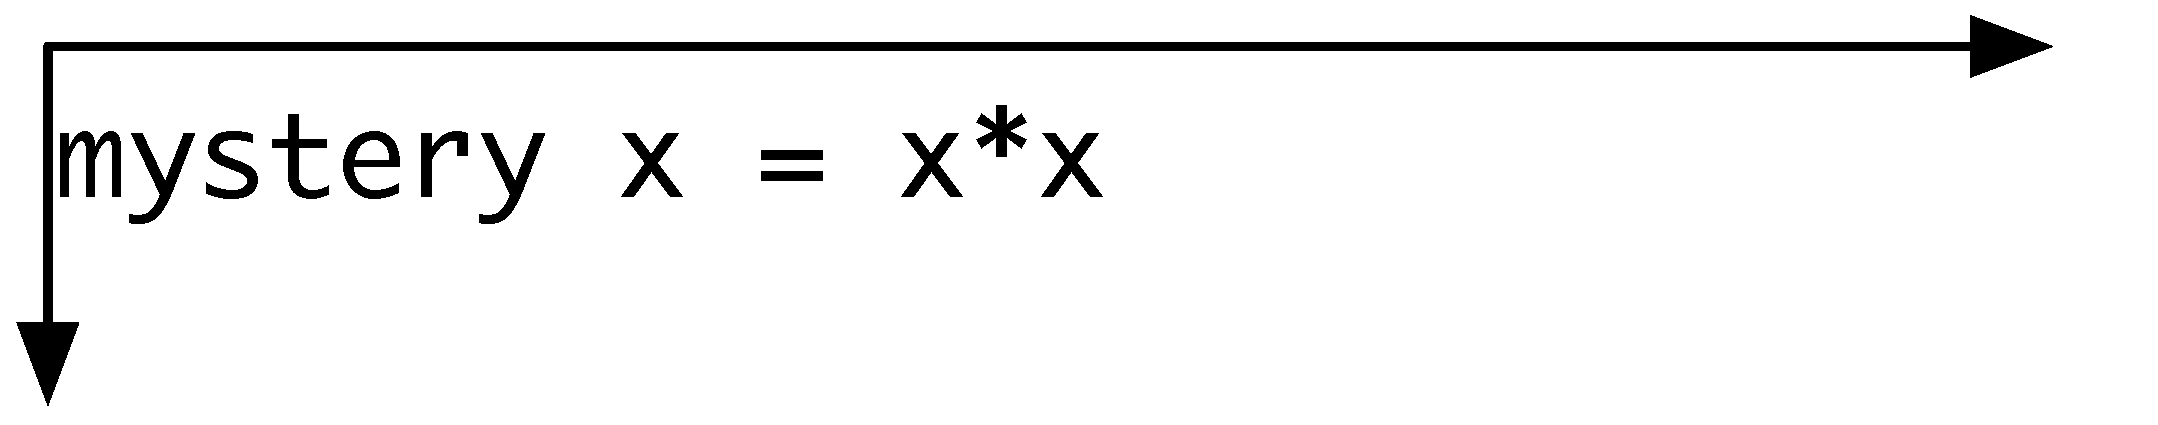
\includegraphics[width=2.3in]{Pictures/mystery1.pdf}
\end{center}
Whatever is typed in the box forms part of the definition \ldots
\begin{center}
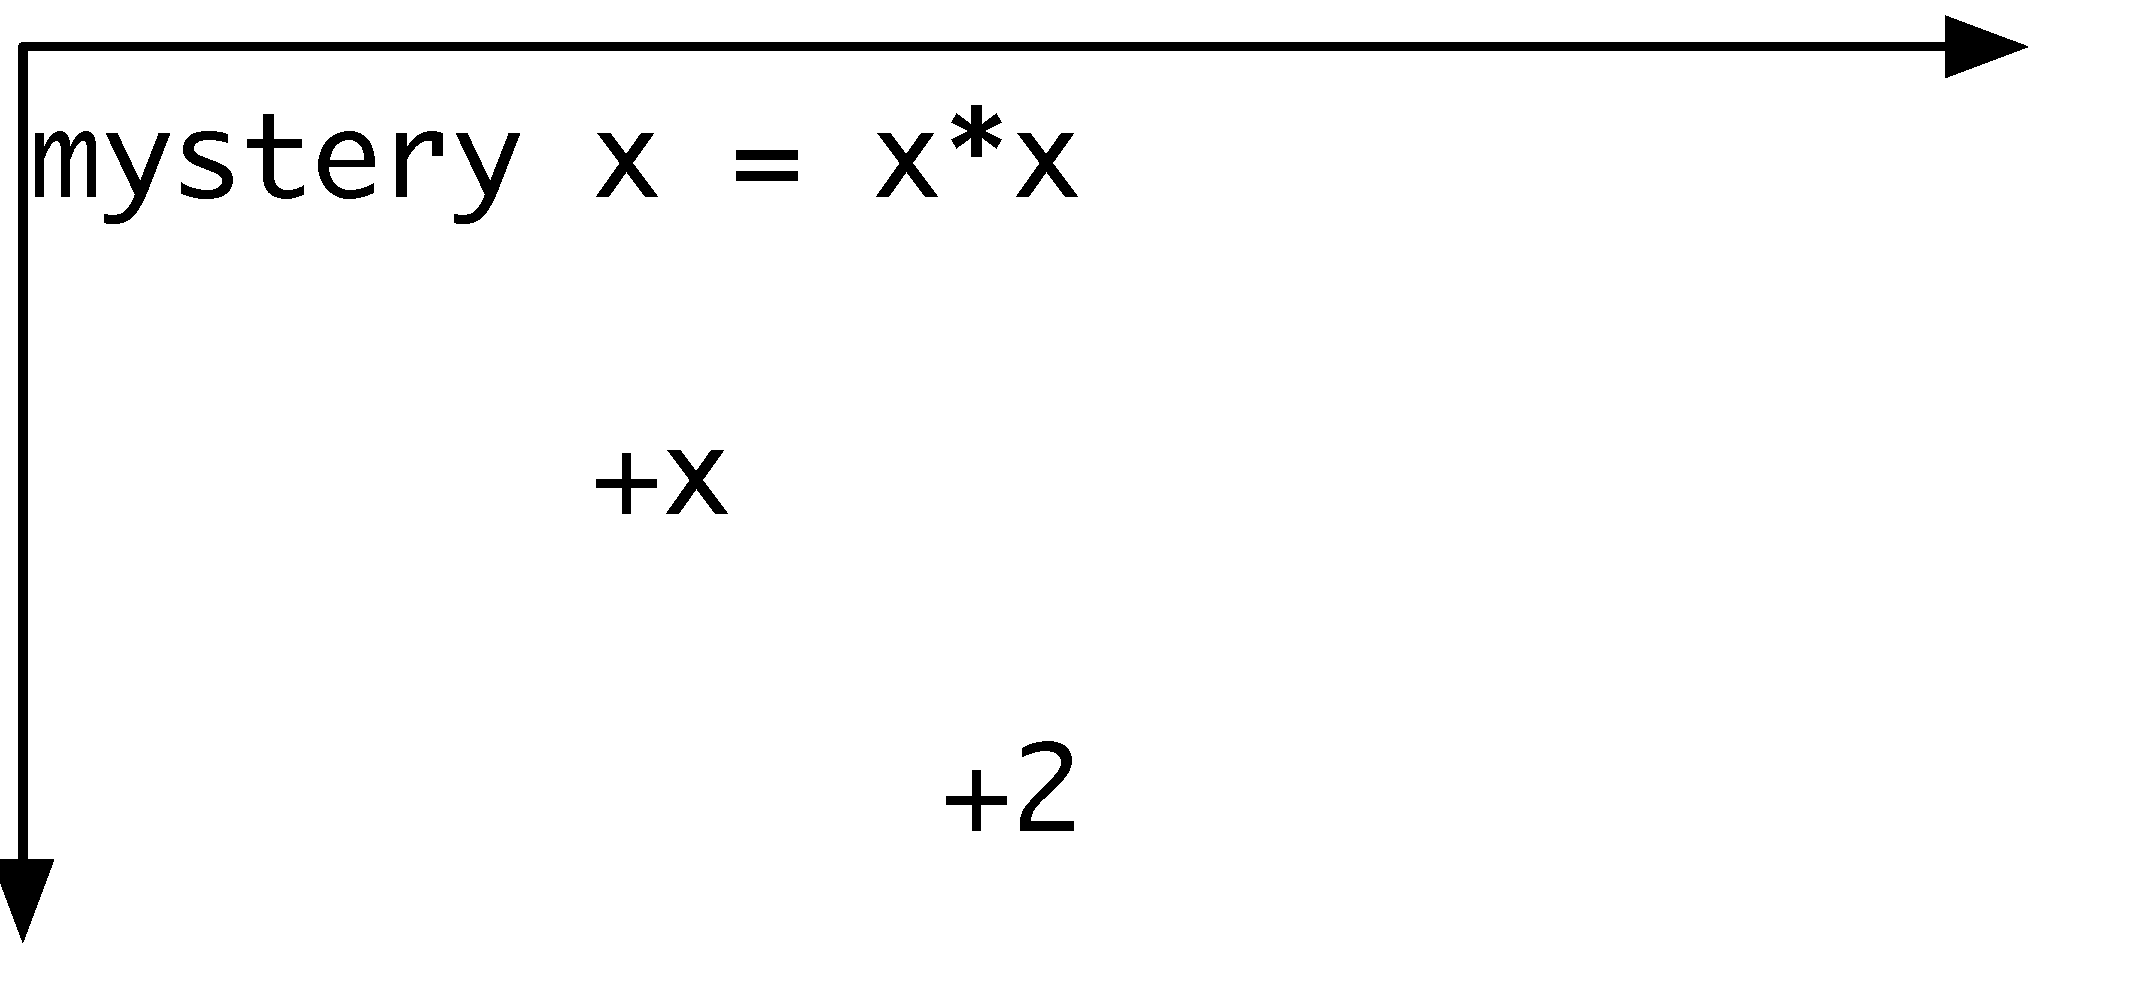
\includegraphics[width=2.3in]{Pictures/mystery2.pdf}
\end{center}
\ldots until something is found which is on the line
or to the left of the line. This
closes the box, like this
\begin{center}
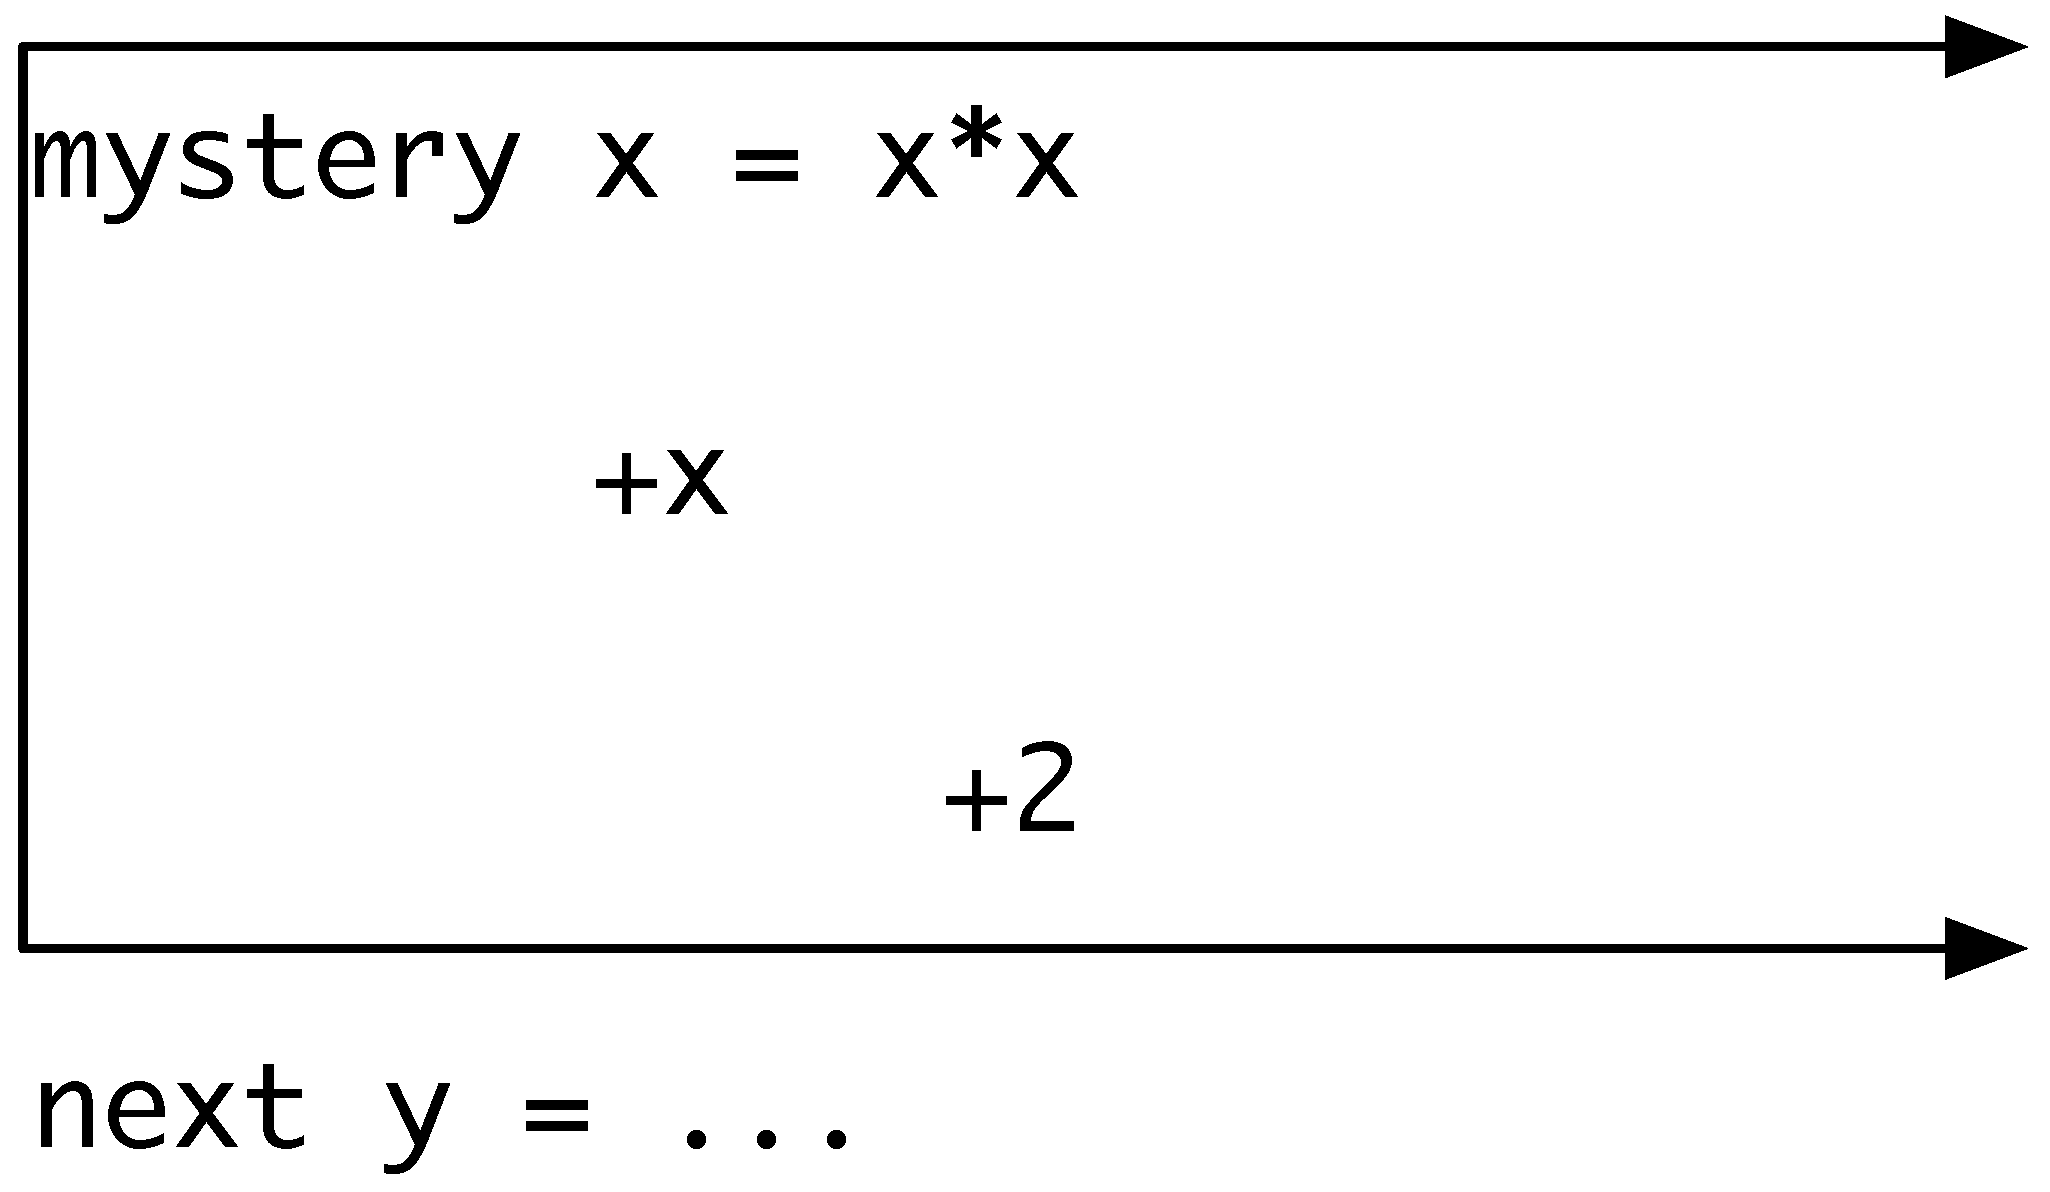
\includegraphics[width=2.3in]{Pictures/mystery3.pdf}
\end{center}
In writing a sequence of definitions, it is therefore sensible to give them
all the same level of indentation. In our scripts we shall always write
top-level definitions starting at the left-hand side of the page, and in
literate scripts we will indent the start of each definition by a single `tab'.

This rule for layout is called the \textbf{offside rule}\index{offside rule}
because it is
reminiscent of the idea of being `offside' in soccer.
The rule also works for conditional equations such as \texttt{max} and
\texttt{maxThree}
which consist of more than one clause.

There is, in fact, a mechanism in Haskell for giving an explicit end to part
of a definition, just as `\texttt{.}' does in English: the Haskell `end' symbol
is `\texttt{;}'. We can, for instance, use `\texttt{;}' if we wish to write more
\minx{;}
than one definition on a single line, thus:
\begin{alltt}
answer = 42 ;   facSix = 720 
\end{alltt}

\begin{figure}\index{errors!layout}
\beware{Layout errors}{\index{pitfalls!\texttt{;} in error message}%
If we break the offside rule like this:
\begin{alltt}
funny x = x+\\
1
\end{alltt}
we receive an error message like this:
\begin{alltt}
Chapter3.hs:33:0:

\ \ \ \ parse error (possibly incorrect indentation)
    
Failed, modules loaded: none.
\end{alltt}
which indicates that the indentation may well be the problem. The position 33:0 is the position of the digit \texttt{1}, which is in \emph{row} 33 and \emph{column} 0 of the file \texttt{Chapter3.hs}.
\index{errors!offside rule}
}\end{figure}

\subsection*{Recommended layout}
\index{layout!recommended}

The offside rule permits various different styles of layout. In this book 
for definitions of any size we use the form 
\begin{alltt}
fun \vone \vtwo \ldots \vn
  | \gone          = \eone     
  | \gtwo          = \etwo   
  \ldots
  | otherwise   = \er       ({\rm or}    | \gr      = \er)
\end{alltt}
for a \textbf{conditional equation}\index{conditional equation} built up
from a number of clauses.
In this layout, each \textbf{clause} starts on a new line, and the guards and results
\index{clause}
are lined up. Note also that by convention in this text we always specify the type
of the function being defined.
\index{conventions!types specified}

If any of
the expressions \texttt{\ei} or guards \texttt{\gi} is particularly long, then the
\index{guard}
guard can appear on a line (or lines) of its own, like this
\begin{alltt}
fun \vone \vtwo \ldots \vn
  | a long guard which may
    go over a number of lines 
       = very long expression which goes 
         over a number of lines
  | \gtwo       = \etwo         
  \ldots
\end{alltt}
If you use an editor which is Haskell-aware, e.g. emacs with Haskell mode, then the editor will help you to indent your code. In this particular case, hitting the tab key repeatedly will cycle through a set of suggested indentations of the line that you are currently working on, based on its contents.


\subsection*{Names in Haskell}

Thus far in the book we have seen a variety of uses of names in definitions
and expressions. In a definition like
\begin{alltt}
addTwo :: Int -> Int -> Int
addTwo first second = first+second
\end{alltt}
the names or \textbf{identifiers} \index{name}\index{identifier}
\texttt{Int}, \texttt{addTwo}, \texttt{first} and \texttt{second} are used to
name a type, a function and two variables. Identifiers in Haskell must begin
with a letter -- small or capital -- which is followed by an optional
sequence of letters, digits, underscores `\verb+_+' and single quotes.

The names used in definitions of values must
begin with a small letter, as must variables
and type
variables, which are introduced later. On the other hand, 
capital letters are used to begin
type names, such as \texttt{Int}; \textbf{constructors}\index{constructor}, such as
\texttt{True} and \texttt{False}; module names and also the names of  
type classes, which we shall encounter
below.

An attempt to give a function a name
which begins with a capital letter, such as
\begin{alltt}
Funny x = x+1
\end{alltt}
gives the error message:
\begin{alltt}
Chapter3.hs:32:0:
\ \ \ \ Not in scope: data constructor `Funny'
\end{alltt}
There are some restrictions on how identifiers can be chosen. There is
a small collection of \textbf{reserved words} which cannot be used; these
are\index{reserved words}
\begin{alltt}
case class data default deriving do else if import in infix
infixl infixr instance let module newtype of then type where
\end{alltt}
The special identifiers \texttt{as}, \texttt{qualified}, and
\texttt{hiding}\minx{as}\minx{qualified}\minx{hiding} 
have special meanings in certain contexts but can be
used as ordinary identifiers.

By convention, when we give names built up from more than one word, we
capitalize the first letters of the second and subsequent words, as in 
`\texttt{maxThree}'.
\index{conventions!capitalizing internal words}

The same identifier can be used to name both
a function and a variable, or both a type
and a type constructor; we recommend strongly that this is {\em not\/} done,
as it can only lead to confusion. 

If we want to \textbf{redefine} a name that is
already defined in the prelude or one of the libraries we have to \textbf{hide} that name on
import; details of how to do this are given on page \pageref{redefName}.

Haskell is built on top of the Unicode\index{characters!Unicode} character
description standard, which allows symbols from fonts other than those
in the ASCII standard.
These symbols can be used in identifiers and the like, and
Unicode characters -- which are described by a 16-bit sequence -- can be input 
to Haskell in the form \texttt{\bs{u}}\textit{hhhh} where each of the \textit{h} is a
hexadecimal (4 bit) digit. In this text we use the ASCII subset of
Unicode exclusively. 

\subsection*{Operators}
\label{operators}
\index{operator|(}

The Haskell language contains various operators, like \texttt{+}, \texttt{++} and
so on. Operators are \textbf{infix} functions, so that they are written between their
\index{operator!infix}
arguments, rather than before them, as is the case for ordinary functions. 

In principle it is possible to write all applications of an
operator with enclosing parentheses, thus
\begin{alltt}
(((4+8)*3)+2)
\end{alltt}
but expressions rapidly become difficult to read. Instead two extra
properties of operators allow us to write expressions uncluttered by
parentheses.

\subsubsection*{Associativity}
\index{operator!associativity of}
\index{associativity}

If we wish to add the three numbers \texttt{4}, \texttt{8} and \texttt{99} we can write
either \texttt{4+(8+99)} or \texttt{(4+8)+99}. The result is the same whichever we
write, a property we call the \textbf{associativity} of addition. Because of
this, we can write 
\begin{alltt}
4+8+99
\end{alltt}
for the sum, unambiguously. Not every operator is associative, however; what
happens when we write
\begin{alltt}
4-2-1
\end{alltt}
for instance? 
The two different ways of inserting parentheses give
\begin{alltt}
(4-2)-1 = 2-1 = 1\hfill{\rm left associative}
4-(2-1) = 4-1 = 3 \hfill{\rm right associative}
\end{alltt}
\index{associativity!left/right}
In Haskell 
each non-associative operator is classified as either left or right
associative. If left associative, any double occurrences of the operator
will be parenthesized to the left; if right associative, to the right. The
choice is arbitrary, but follows custom as much as possible, and in
particular `\texttt{-}' is taken to be left associative.

\subsubsection*{Binding powers}
\index{operator!binding power of}
 
The way in which an operator associates allows us to resolve expressions like
\begin{alltt}
2\^{}3\^{}2
\end{alltt}
where the same operator occurs twice, but what is done when two different
operators occur, as in the following expressions?
\begin{alltt}
2+3*4
3\^{}4*2
\end{alltt}
For this purpose the \textbf{binding power} or \textbf{fixity}
of the operators\index{fixity}\index{binding power}
need to be compared. \texttt{*} has binding power 7 while \texttt{+} has 6, so
that in \texttt{2+3*4} the \texttt{3} sticks to the \texttt{4} rather than the {\mi
2}, giving

\begin{alltt}
2+3*4 = 2+(3*4)
\end{alltt}
In a similar way, \texttt{\^{}} with binding power 8
binds more tightly than \texttt{*}, so

\begin{alltt}
3\^{}4*2 = (3\^{}4)*2
\end{alltt}
A full table of the associativities and binding powers of the predefined
Haskell operators is given in Appendix \ref{hsOps}. 
In the section `Do-it-yourself operators' below we discuss how
operators are defined in scripts and also how their associativity and binding
power can be set or changed by declarations. 

\begin{figure}[t]
\beware{Function application}{\index{function application}%
\index{pitfalls!function application}
Binding most tightly is function application, which is given by writing the
name of the function in front of its argument(s) thus:
\texttt{f \vone\ \vtwo\ \ldots\ \vn}. This binds more tightly than any other
operator, so that \texttt{f n+1} is interpreted as \texttt{f n} plus 
\texttt{1}, \texttt{(f n)+1}, rather than \texttt{f} applied to \texttt{n+1}, \texttt{f (n+1)}. 
If in doubt, it is sensible to
parenthesize each argument to a function application.

\medskip
Similarly, as `\texttt{-}' is both an infix and a prefix operator, there is
scope for confusion. \texttt{f -x} will be interpreted as \texttt{x} subtracted
from 
\texttt{f}, rather than \texttt{f} applied to \texttt{-x}; the solution again is to
bracket the argument, giving \texttt{f (-x)}.
}\end{figure}

\subsubsection*{Operators and functions}

Infix operators can be  written {\em before\/}
their arguments, by enclosing the operator in parentheses. We therefore have,
for example,
\begin{alltt}
(+) :: Integer -> Integer -> Integer
\end{alltt}
so that
\begin{alltt}
(+) 2 3 = 2 + 3
\end{alltt}
This conversion is needed later when we make functions into
arguments of other functions.
We can also convert functions into operators by enclosing the function name in
backquotes, thus \texttt{`name`}. We therefore have, using the maximum function
defined earlier,

\begin{alltt}
2 `max` 3 = max 2 3
\end{alltt}
This notation can make expressions involving \textbf{binary}\index{function!binary} or two-argument functions substantially easier to read.

The fixity and associativity of these operators can be controlled; see
Appendix \ref{hsOps}.

\subsubsection*{Do-it-yourself operators}
\index{operator!definitions of}

The Haskell language allows us to define infix operators directly in exactly the same way
as functions.
Operator names are built from the operator symbols which include the
ASCII symbols

\begin{alltt}
! \# \$ \% \& * + . / < = > ? \@ \bs{} \^{} | : - \twid
\end{alltt}
together with the Unicode symbols. An operator name may not begin with a
colon.

To define the operator \texttt{\&\&\&} as an integer minimum function, we
write

\begin{alltt}
(\&\&\&) :: Integer -> Integer -> Integer\minx{\&\&\&}
x \&\&\& y 
  | x > y       = y
  | otherwise   = x
\end{alltt}
The associativity and binding power of the operator can be specified; for details
see Appendix \ref{hsOps}.
\index{operator|)}
\index{syntax|)}

\begin{exercises}

\item Rewrite your solutions to the earlier exercises to use the recommended
layout.

\item Given the definitions
\begin{alltt}
funny x = x+x
 peculiar y = y
\end{alltt}
explain what happens when you remove the space in front of the {\mi
peculiar}.
\end{exercises}

\begin{summary}
This chapter has introduced the base types \texttt{Integer}, \texttt{Int}, \texttt{Float},
\texttt{Char} and \texttt{Bool} together with various built-in functions over them.
We have seen how Boolean expressions -- called guards -- allow
definitions which have various cases, and this was exemplified by the function
returning the maximum of two integer arguments. This definition contains two
cases, one which applies when the first argument is the larger and the other when the second is the larger.

Finally, we have seen how the layout of a Haskell program is
significant -- the end of a definition is implicitly given by the first
piece of program text `offside' of the start of the definition;  we
have also given an overview of operators in Haskell.

This material, together with what we have seen in earlier chapters,
gives us a toolkit which we can use to solve programming problems. In
the next chapter we will explore various ways of using that toolkit to
solve practical problems.
\end{summary}
%\end{document} 



%\documentclass{book}\usepackage{sjtfonts}\usepackage{includegraphics}\usepackage{alltt}\usepackage{latexsym}
%\begin{document}\input{defs0}%		miradefs.tex 		    June 1994

% opening and closing a quoted Miranda section

\newcommand{\mira}{\noindent\hrulefill\nopagebreak\so}
\newcommand{\arim}{\nopagebreak\st\hrulefill\\}

% backslash in the Miranda environment
% Only feasible approach is to use \verb+\+
% in line!

%\newcommand{\bs}{$\mi\backslash\!\!$}
%\newcommand{\lbs}{\mbox{\verb+\+}}

% ignoring part of the input

\newcommand{\ignore}[1]{}

% a blank line in a Miranda section

\newcommand{\bl}{\mbox{\ }}

% Signalling a diffculty.

\definecolor{light-gray}{gray}{0.95}

\newcommand{\beware}[2]
 {\medskip\noindent\colorbox{light-gray}{\parbox{\textwidth}
 {\mbox{\large\textbf{#1}} \medskip\noindent\\ #2}\medskip\noindent}}

% Subscripting in Miranda text
\newcommand{\subscr}[2]{\mbox{${\mbox{\texttt{#1}}}_{\mbox{\texttt{#2}}}$}}

%\newcommand{\subscr}[2]{\mbox{${\mbox{\mi #1}}_{\mbox{\smtt #2}}$}}
\newcommand{\aone}{\subscr{a}{1}}
\newcommand{\atwo}{\subscr{a}{2}}
\newcommand{\ak}{\subscr{a}{k}}

\newcommand{\aoneone}{\subscr{a}{1,1}}

\newcommand{\eone}{\subscr{e}{1}}
\newcommand{\etwo}{\subscr{e}{2}}
\newcommand{\ei}{\subscr{e}{i}}
\newcommand{\er}{\subscr{e}{r}}

\newcommand{\fone}{\subscr{f}{1}}
\newcommand{\fl}{\subscr{f}{l}}

\newcommand{\gone}{\subscr{g}{1}}
\newcommand{\gtwo}{\subscr{g}{2}}
\newcommand{\gi}{\subscr{g}{i}}
\newcommand{\gr}{\subscr{g}{r}}

\newcommand{\hone}{\subscr{h}{1}}
\newcommand{\hl}{\subscr{h}{l}}

\newcommand{\pone}{\subscr{p}{1}}
\newcommand{\ptwo}{\subscr{p}{2}}
\newcommand{\pk}{\subscr{p}{k}}

\newcommand{\qone}{\subscr{q}{1}}
\newcommand{\qtwo}{\subscr{q}{2}}
\newcommand{\qk}{\subscr{q}{k}}

\newcommand{\rone}{\subscr{r}{1}}
\newcommand{\rtwo}{\subscr{r}{2}}

\newcommand{\tone}{\subscr{t}{1}}
\newcommand{\ttwo}{\subscr{t}{2}}
\newcommand{\tn}{\subscr{t}{n}}

\newcommand{\vone}{\subscr{v}{1}}
\newcommand{\vtwo}{\subscr{v}{2}}
\newcommand{\vn}{\subscr{v}{n}}

% for regular expressions

\newcommand{\stone}{\subscr{st}{1}}
\newcommand{\sttwo}{\subscr{st}{2}}
\newcommand{\stn}{\subscr{st}{n}}
\newcommand{\rthree}{\subscr{r}{3}}

\newcommand{\eps}{$\varepsilon$}
\newcommand{\trans}[1]{\stackrel{\mbox{\tt #1}}{\longrightarrow}}



% superscript in Miranda text

\newcommand{\superscr}[2]{\mbox{${\mbox{\mi #1}}^{\mbox{\smtt #2}}$}}

% Not equals in Miranda text

\newcommand{\noteq}{\makebox[0pt][l]{=}/}
\newcommand{\overslash}{\makebox[0pt][l]{/}}

% Definitions in complexity chapter

\newfont{\oldSym}{cmsy10}
\newcommand{\Th}{\boldmath$\oldSym\Theta$}
\newcommand{\pow}[1]{\^{}#1}
\newcommand{\leqq}{$\leq$}
\newcommand{\geqq}{$\geq$}
\newcommand{\lll}{$\ll$}
\newcommand{\eqq}{$\equiv$}
\newcommand{\ltwo}{\subscr{log}{2}}

% Indexing

\newcommand{\minx}[1]{\index{#1@{\ttfamily{}#1}}}


\chapter{Designing and writing programs}
\chapstart
\label{writingProgs}


\medskip
In this chapter we step back from discussing the details of Haskell and
instead look at how to build programs. We present some general strategies
for program design; that is we talk about how programs can be planned
{\em before\/} we start to write the details.
The advice we give here is largely independent of
Haskell and will be useful whatever programming language we use. 


Two particular aspects of Haskell help with program design, and we introduce each of these in this chapter. First, we talk about \textbf{local definitions}, which we can use in solving problems -- that is defining functions -- step by step. Secondly we start our discussion of how to define types for ourselves, using Haskell \texttt{data} types.


We follow this by discussing recursion. We begin by concentrating on explaining \textbf{why} 
recursion works, and follow this by looking at \textbf{how} to find primitive recursive
definitions, extending what we have said about design. We conclude with
an optional examination of more general forms of recursion.

Once we have written a definition we need to ask whether it does what it is
intended to do. We conclude the chapter by discussing the principles of program
testing and examining a number of examples. We use the unit testing framework \textbf{HUnit} as well as \textbf{QuickCheck} for presenting and performing tests. 


\section{{\em Where do I start?} Designing a program in Haskell}
\label{designProgram}
\label{probSolvIntro}
\index{design!where do I start?|(}

One theme which we want to emphasize in this book is how we can
\textbf{design}\index{design} programs to be written in Haskell. 
Design is used to mean many different
things in computing; the way that we want to think of it is like this:
\begin{definition}
{Design is the
stage before we start writing detailed Haskell code.}
\end{definition} 
In this section we will concentrate on looking at examples, and on talking
about the different ways we can try to define functions, but we will
also try to give some general advice about how to start
writing a program. These are set out as questions we can ask ourselves when we are stuck
with a programming problem.

\subsection*{Do I understand what I need to do?}

Before we can start to solve a programming problem we need to be clear
about what we have to do. Often problems are described in an informal way, and
this can mean that the problem either is not fully stated or cannot be
solved as it is described.

Suppose we are asked to return the middle of three numbers. It is clear
that given the numbers \texttt{2}, \texttt{4} and
\texttt{3} we should return \texttt{3}, but when presented with \texttt{2}, \texttt{4} and
\texttt{2} there are two possible responses.
\begin{itemize}
\item\label{middleNumb}
We could say that \texttt{2}
is the middle number because when we write the numbers in order: \texttt{2 2 4}, 
then \texttt{2} 
is the number that appears in the middle.
\item
Alternatively we could say that there is no middle number in this case,
since \texttt{2} is the lower and \texttt{4} the higher,
and that we therefore cannot return any result.
\end{itemize}
What can we learn from this illustration? 
\begin{itemize}
\item
First, that even in simple
problems there can be things we have to think about before we start programming.
\item
Secondly, it is important to realize that there is \textbf{no right answer} among the two options 
given just now: it is up to the person wanting the program written and
the programmer to work out between them what is wanted. 
\item
Thirdly, a very
good way of thinking about whether we understand the problem is to think
about how we expect it to work out in various \textbf{examples}.
\item
Finally, it is worth realizing that often difficulties like this come
out at the programming stage, when we have already written a whole lot
of definitions; the sooner we spot a problem like this, the more wasted effort
we can save.
\end{itemize}
Another example of this came up in the definition of \texttt{max}
in Section \ref{guards}, where we had to say what the function should
return when its two arguments were the same. In that case it was
sensible to think of the maximum of, say, 
\texttt{3} and \texttt{3} as being \texttt{3}.

\subsection*{Can I say anything about types at this stage?}
\index{design!types}

One thing we can think about at this stage is the types of the various
things we are thinking about. We can write
\begin{alltt}\minx{middleNumber}
middleNumber :: Integer -> Integer -> Integer -> Integer 
\end{alltt}
as the name and type of the function returning the middle of three
numbers without having any idea about how we are going to define the
function itself. Nevertheless, it is progress, and also it gives us
something to check our definition against when we have written it: if we
manage to write a function \texttt{middleNumber} but it does not have
the type \texttt{Integer -> Integer -> Integer -> Integer}, then the function cannot be
doing what it should.


It might be that the built-in types of Haskell don't suit the problem: we can then think of defining types for ourselves. We'll begin to do that in Section \ref{EnumTypes}.

\subsection*{What do I already know? How can I use this information?}

These are crucial questions for a designer of a program. We need to
know what resources are available to us for solving the problem at hand:
what definitions have we already written which could be useful, what
does the language provide in its prelude and libraries? We will
obviously learn more about the latter as we go along, but even when we
have written only
a small number of programs we should always think about how
these might help us solve the problem at hand. For instance, in trying to define the
function 
\texttt{maxThree} introduced in Section \ref{guards}, we know that we have already got the
\texttt{max} function, giving the maximum of two numbers.

As well as knowing our resources we also need to know how we can use
them; this we look at now. There are two different ways that a
definition we already have can be helpful.

\subsubsection*{We can take the {definition} {of} a function as a {\bfseries
model\/} for what we want to  do}

In defining \texttt{maxThree}\minx{maxThree} we have the resource of already having defined
the function \texttt{max}. We can think of its definition as a model for how we might 
define \texttt{maxThree}.

In \texttt{max} we give the result \texttt{x} on condition that it is
the maximum of the two, that is
\begin{alltt}
x >= y
\end{alltt} 
Our definition of \texttt{maxThree} does a similar thing, replacing the condition
for two values with the condition for three, namely:
\begin{alltt}
x >= y \&\& x >= z
\end{alltt}
This way of using \texttt{max} is probably the first to spring to mind,
but it is not the only way that \texttt{max} can help us in defining
\texttt{maxThree}. 

\subsubsection*{We can {\bfseries use\/} a function we have already
defined within the new definition}

We are trying to find the maximum of three numbers, and we are already
provided with a function \texttt{max} to give us the maximum of two. How
could we {\em use\/} \texttt{max} to give us the result we want? We can
take the maximum of the first two, and then the maximum of that and the
third. In pictures,
\begin{center}
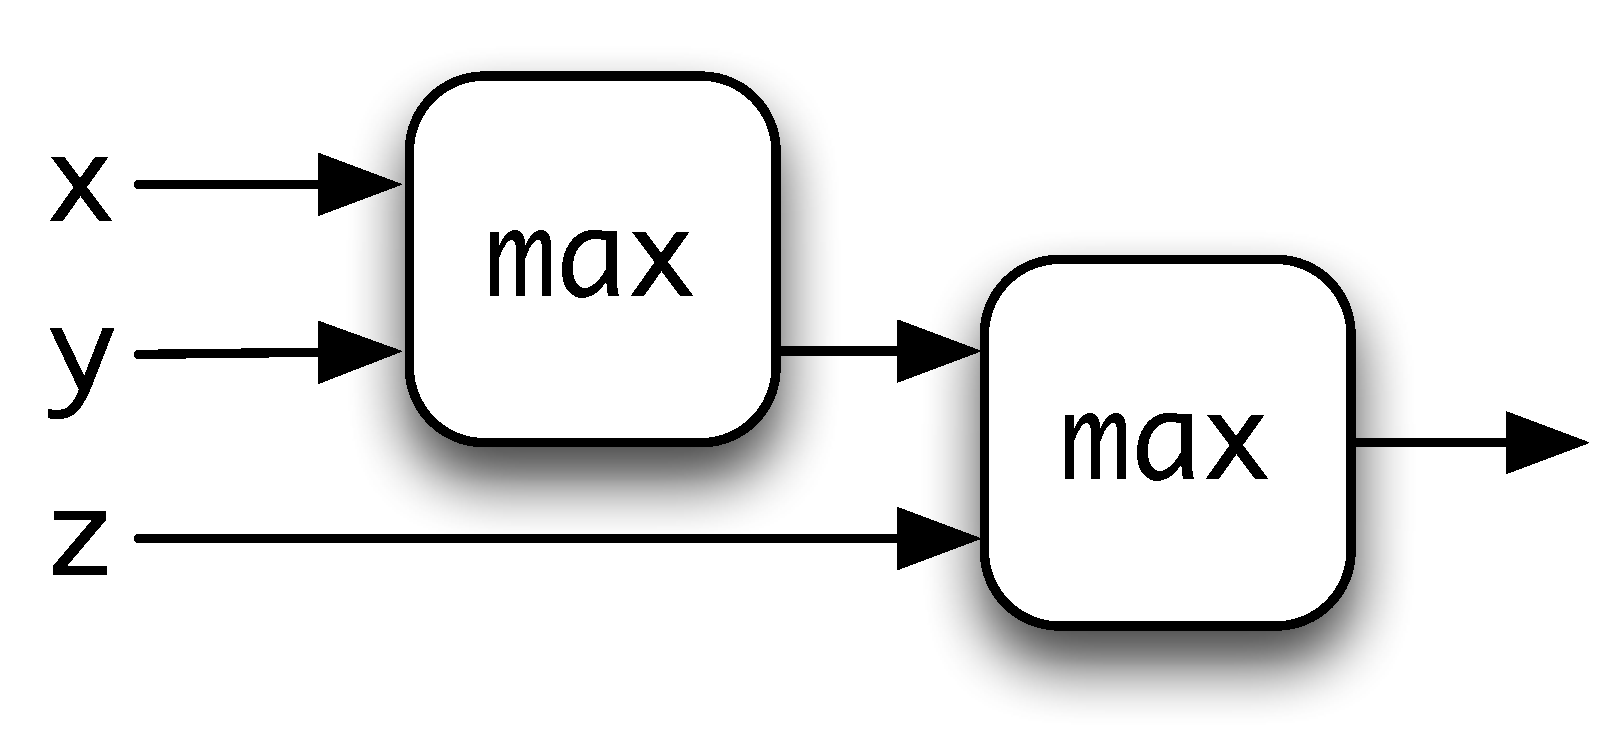
\includegraphics[width=3in]{Pictures/maxThree.pdf}
\end{center} 
and in Haskell
\begin{alltt}
maxThree x y z = max (max x y) z
\end{alltt}
or writing the \texttt{max} in its infix form, \texttt{`max`},
\begin{alltt}
maxThree x y z = (x `max` y) `max` z
\end{alltt}
Using \texttt{max} in this way has some advantages. 

The definition of
\texttt{maxThree} is considerably shorter and easier to read than the
original. If at some point we changed the way that \texttt{max} was
calculated -- perhaps making it a built-in function -- then this
definition would get the benefit of the `new' \texttt{max}. This is not
such an advantage in a small example like this, but can be of
considerable benefit in a larger-scale system where we can expect
software to be modified and extended over its lifetime.

\subsection*{Can I break the problem down into simpler parts?}

If we cannot solve a problem as it stands, we can think about breaking it
down into smaller parts. This principle of `divide and conquer'\index{divide and conquer}
\index{design!divide and conquer} is the
basis of all larger-scale programming: we solve aspects of the problem
separately and then put them together to give an overall solution.

How do we decide how to break a problem down into parts? We can think of
solving a simpler problem and then building the full solution on top, or
we can ask ourselves the question here.

\subsubsection*{{\bfseries What if\/} I had any functions I wanted: which could I use in
writing the solution?} 
\index{design!what if?}

This {\em what if \ldots?\/} is a central question, because it breaks the problem into two
parts. First we have to give the solution {\em assuming\/} we are
given the auxiliary functions we want and thus without worrying about how they are
to be defined. Then, we have separately to define these
auxiliary functions. 
\begin{center}
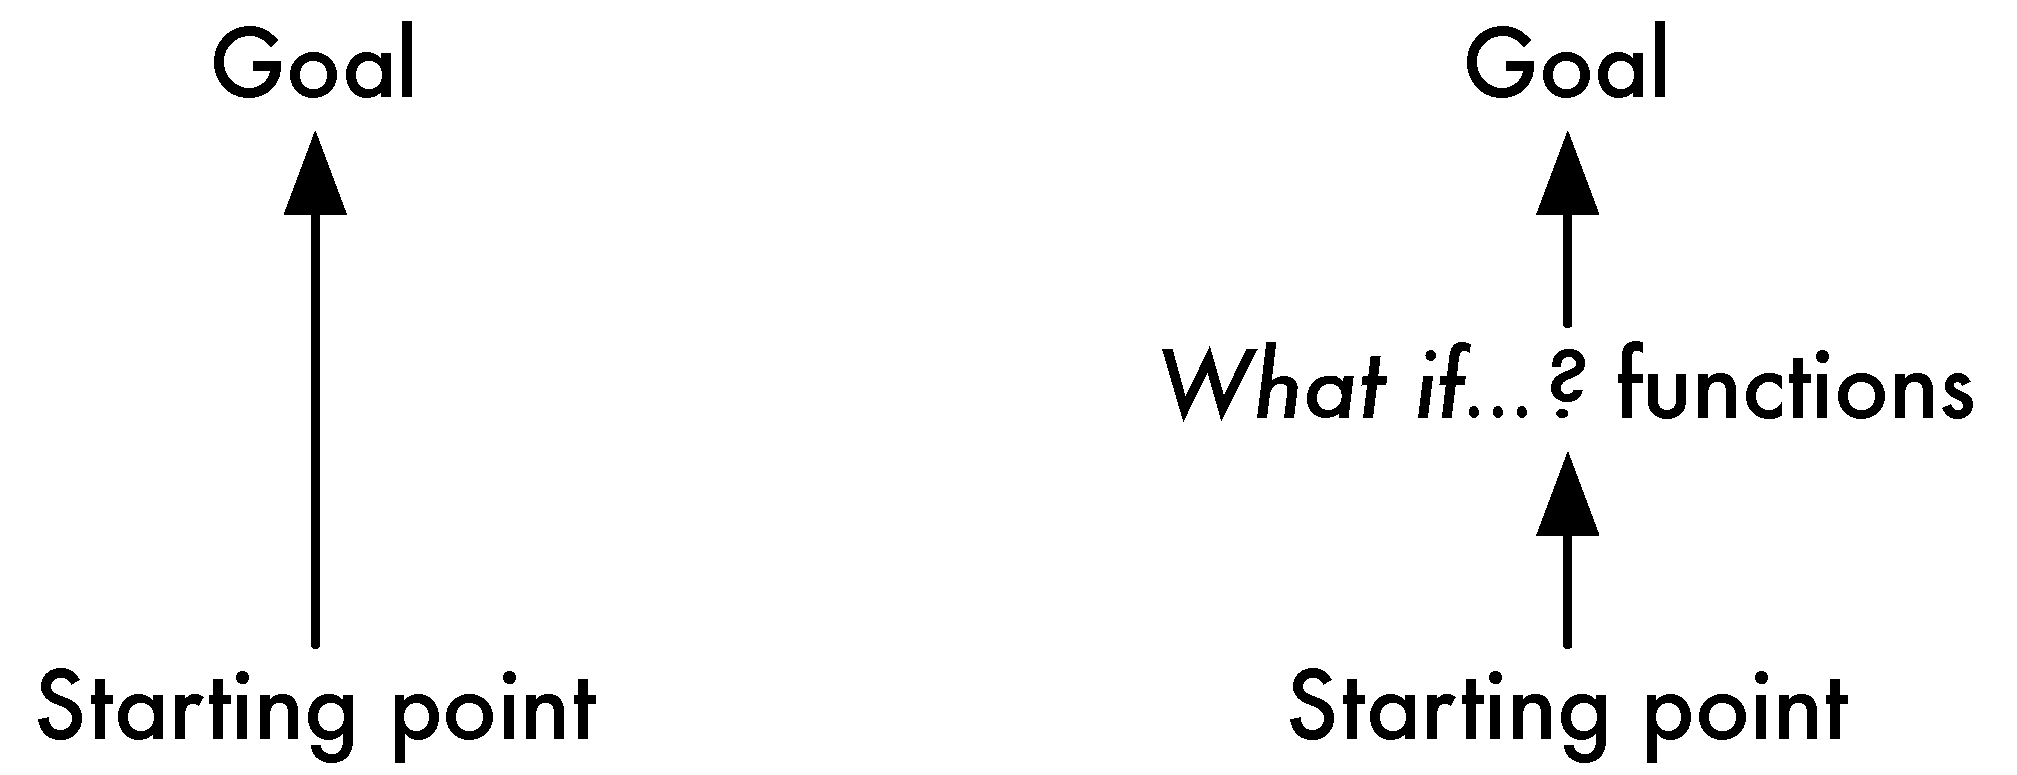
\includegraphics[width=3.5in]{Pictures/whatIf.pdf}
\end{center}
Instead of a single jump from the starting point to the goal, we have
two shorter jumps, each of which should be
easier to do. This approach is called \textbf{top-down}\index{design!top-down}
as we start at the top with the overall problem, and work by breaking it down into smaller
problems. 

This process can be done repeatedly, so that the overall problem is solved in a series
of small jumps.\index{design!iterative} We now look at an example; more examples appear in the exercises at the end
of the section.

Suppose we are faced with the problem of defining
\begin{alltt}\minx{middleNumber}
middleNumber :: Integer -> Integer -> Integer -> Integer 
\end{alltt}
according to the first of the alternatives described on page
\pageref{middleNumb}. A model is given by the definition of
\texttt{maxThree}, in which we give conditions for \texttt{x} to be the
solution, \texttt{y} to be the solution and so on. We can therefore
sketch out our solution like this
\begin{alltt}
middleNumber x y z
  | condition for x to be solution      = x
  | condition for y to be solution      = y
  ....
\end{alltt}
Now, the problem comes in writing down the conditions, but here we say
{\em what if\/} we had a function to do this. Let us call it
\texttt{between}. It has three numbers as arguments, and a Boolean
result, 
\begin{alltt}\minx{between}
between :: Integer -> Integer -> Integer -> Bool
\end{alltt}
and is defined so that \texttt{between m n p} is \texttt{True} if \texttt{n} is
between \texttt{m} and \texttt{p}. We can complete the definition of
\texttt{middleNumber} now:
\begin{alltt}
middleNumber x y z
  | between y x z      = x
  | between x y z      = y
  | otherwise          = z
\end{alltt}
The definition of the function \texttt{between} is left as an exercise for the reader.

This section has introduced some of the general ideas which can help us
to get started in solving a problem. Obviously, because programming is a creative
activity  there is not going to be a set of rules
which will always lead us mechanically to a solution to a problem. On
the other hand, the questions posed here will get us started, and show
us some of the alternative strategies we can use to plan how we are
going to write a program. 

We'll follow this up in the next section, where we look at another way we can break problems down and solve them in steps. After that we'll take a first look at how to define our own data types in solving problems. We take up the discussion again in Chapter \ref{moreDesign}.

\begin{exercises}

\item
This question is about the function
\begin{alltt}
maxFour :: Integer -> Integer -> Integer -> Integer -> Integer
\end{alltt}
which returns the maximum of four integers. Give three definitions of this
function: the first should be modelled
on that of \texttt{maxThree}, the second should use the function
\texttt{max} and the third should use the functions \texttt{max} and
\texttt{maxThree}. For your second and third solutions give diagrams
to illustrate your answers. Discuss the relative merits of the three
solutions
you have given.

\item
Give a definition of the function 
\begin{alltt}
between :: Integer -> Integer -> Integer -> Bool
\end{alltt}
discussed in this section. The definition should be consistent with what we said
in explaining how \texttt{middleNumber}
works. You also need to think carefully about the different ways that
one number can lie between two others. You might find it useful to
define a function
\begin{alltt}
weakAscendingOrder :: Integer -> Integer -> Integer -> Bool
\end{alltt}
so that \texttt{weakAscendingOrder m n p} is \texttt{True} exactly when
\texttt{m}, \texttt{n} and \texttt{p} are in weak ascending order, that is the sequence
does not go down at any point. An example of such a sequence is 
\texttt{2 3 3}.

\item
Give a definition of the function
\begin{alltt}\minx{howManyEqual}
howManyEqual :: Integer -> Integer -> Integer -> Integer
\end{alltt}
which returns how many of its three arguments are equal, so that
\begin{alltt}
howManyEqual 34 25 36 = 0
howManyEqual 34 25 34 = 2
howManyEqual 34 34 34 = 3
\end{alltt}
Think about what functions you have already seen -- perhaps in the exercises --
which you can use in the solution.

\item
Give a definition of the function
\begin{alltt}
howManyOfFourEqual :: Integer -> Integer -> Integer -> Integer -> Integer
\end{alltt}
which is the analogue of \texttt{howManyEqual} for four numbers. You may
need to think {\em what if \ldots?}.
\index{design!where do I start?|)}
\end{exercises}


\section{Solving a problem in steps: local definitions}
\label{intro-localdefs}\label{localDefs}\index{definition!local|(}

In this section we'll look at a way that we can make \emph{local} definitions as a part of making a function definition: these might be definitions of useful functions, or of values which we can use in defining our answers. We start by looking at some examples, and then discuss some of the details of the \texttt{where} and \texttt{let} constructs.

\subsection*{Examples}

\vspace*{-1cm}
\begin{wrapfigure}[5]{r}{3.5cm}
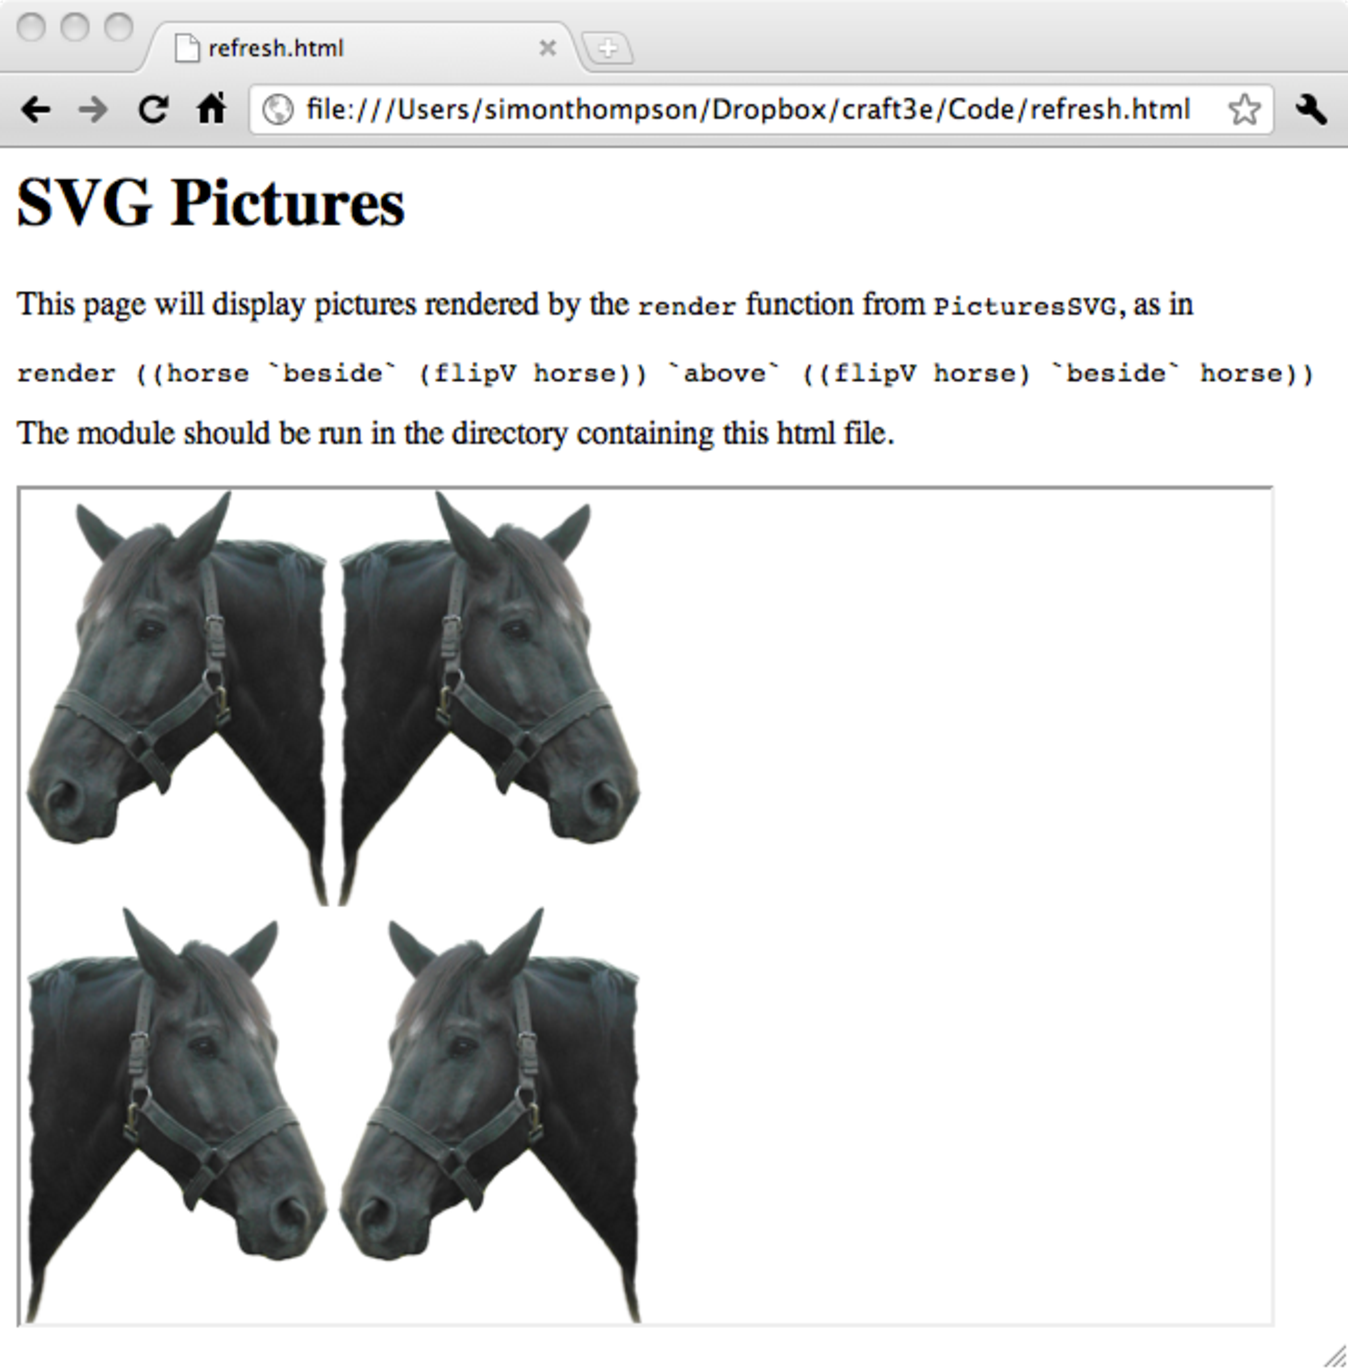
\includegraphics[width=3.5cm]{Pictures/ScreenSVG.pdf}
\end{wrapfigure}
\vspace*{1cm}
The example we will follow is to define a function over pictures, as implemented in the module \texttt{PicturesSVG.hs}. Suppose we want to define a function that takes a picture like horse, and delivers the picture first shown in Figure \ref{svgpix} on page \pageref{svgpix}. 

\medskip
\noindent
One way to tackle it is to start this way:
\begin{alltt}
fourPics :: Picture -> Picture

fourPics pic =
    left `beside` right
      where
        left  = ...
        right = ...
\end{alltt}


\noindent
where we define what \texttt{left} and \texttt{right} mean in the \emph{local definitions} that follow the \texttt{where}. The reason these are called `local' is that they can only be used in the definition of the \texttt{fourPics} function, and nowhere else. 

So, we have broken the problem down into two parts, each simpler than the whole problem. Let's look at the \texttt{left} first. We get this by putting the \texttt{pic} above an inverted version, so giving us
\begin{alltt}\minx{fourPics}\minx{where}
fourPics :: Picture -> Picture

fourPics pic =
    left `beside` right
      where
        left  = pic `above` invertColour pic
        right = ...
\end{alltt}
Now, there are a number of ways of finishing off the definition. Let's look at three of these now.
\begin{itemize}
\item
Let's start by defining \texttt{right} \emph{from scratch}, like this
\begin{alltt}
fourPics :: Picture -> Picture

fourPics pic =
    left `beside` right
      where
        left  = pic `above` invertColour pic
        right = invertColour (flipV pic) `above` flipV pic
\end{alltt}
\item
We could modify this solution so that we \emph{add another local definition} to help us. In this case we define \texttt{flipped} as the original \texttt{pic} flipped in a vertical mirror. We do this because we can use this in defining the right hand side in a similar way to how we defined the left.
\begin{alltt}
fourPics :: Picture -> Picture

fourPics pic =
    left `beside` right
      where
        left    = pic `above` invertColour pic
        right   = invertColour flipped `above` flipped
        flipped = flipV pic
\end{alltt}
\item
We could \emph{use} the definition of \texttt{left} in defining \texttt{right}: we get \texttt{right} from \texttt{left} by reflecting it in a vertical mirror, and then inverting the colour (or the other way around), so giving the definition
\begin{alltt}
fourPics :: Picture -> Picture

fourPics pic =
    left `beside` right
      where
        left  = pic `above` invertColour pic
        right = invertColour (flipV left)
\end{alltt}
\item
Finally, we could  define a \emph{local function}; this is a function we can use only within the definition of \texttt{fourPics}, and not elsewhere. The function \texttt{stack} will put a picture above its inverted version; we'll then use \texttt{stack} in defining the \texttt{left} and \texttt{right} parts of the picture.
\begin{alltt}
fourPics :: Picture -> Picture

fourPics pic =
    left `beside` right
      where
        stack p  = p `above` invertColour p
        left     = stack pic
        right    = stack (invertColour (flipV pic))
\end{alltt}

\end{itemize}
As you can see from this example, there's often more than one way of solving a problem, but a very useful tool in each of these solutions was to use local definitions.

Another more mathematical example is given by a function to calculate the area of a triangle with sides \texttt{a}, \texttt{b} and \texttt{c}. The formula for this is \[\sqrt{\mbox{\texttt{s*(s-a)*(s-b)*(s-c)}}}\]
where \texttt{s} is \texttt{(a+b+c)/2}. As a definition in Haskell this becomes
\begin{alltt}\minx{triArea}
triArea :: Float -> Float -> Float -> Float

triArea a b c 
    | possible   = sqrt(s*(s-a)*(s-b)*(s-c))
    | otherwise  = 0
    where
      s = (a+b+c)/2 
      possible = ... for you to define ...
\end{alltt}
Defining \texttt{possible} is left as an exercise: this value should be \texttt{True} only if it's possible to have a triangle with those sides. Each of the numbers should be positive, and each side should satisfy the \emph{triangle inequality}: the length of the side is less than the sum of the other two sides.


\begin{figure}[t]
\beware{\texttt{let} expressions}{\minx{let}It is also possible to make definitions local to an expression, rather than local to a function clause as for \texttt{where}. For instance,
we can write 
\begin{alltt}
let x = 3+2 in x\^{}2 + 2*x - 4
\end{alltt}
giving the result \texttt{31}. If more than one definition is included in one
line they
need to be separated by semi-colons, thus:
\begin{alltt}\minx{;}
let x = 3+2 ; y = 5-1 in x\^{}2 + 2*x - y
\end{alltt}
We shall find that we use this form only occasionally.}
\end{figure}

\subsection*{Calculation with local definitions}
\index{calculation!local definitions}

We  look at how to calculate with local definitions by taking the example of 
a function which is to
return the sum of the squares of two integers.  
\begin{alltt}
sumSquares :: Integer -> Integer -> Integer\minx{sumSquares}

sumSquares n m 
  = sqN + sqM
    where
    sqN = n*n
    sqM = m*m
\end{alltt}
where the \texttt{where} clause is used to find the two squares.

The way in which calculations are written
can be extended to deal with \texttt{where} clauses. The {\ttfamily
sumSquares} function in the previous section gives, for example
\begin{alltt}
sumSquares 4 3
= sqN + sqM
  where
  sqN = 4*4 = 16
\vertline{30pt}  sqM = 3*3 = 9
= 16 + 9
= 25
\end{alltt}
The values of the local definitions are calculated beneath the \texttt{where} if
their values are needed. All local evaluation below the \texttt{where} is indented. To
follow the top-level value, we just have to look at the calculation at the
left-hand side.

The vertical lines which appear are used to link the successive steps of
a
calculation when these have intermediate \texttt{where} calculations. The lines
can be omitted.

\index{definition!local|)}


\subsection*{Layout}

In definitions with \texttt{where} clauses, the layout is significant. The 
offside rule\index{offside rule} is
used by the 
system to determine the end of each definition in the \texttt{where} clause. 

The \texttt{where} clause
must be found in the definition to which it belongs, so that the \texttt{where}
must occur somewhere to the right of the start of the definition. Inside the
\texttt{where} clause, the same rules apply as at the top level: it is therefore
important that the definitions are aligned vertically -- if not, an error will
result.
Our recommended layout is therefore
\index{layout!recommended}
\index{function definition!layout|see{layout}}
\index{function definition!general form}
\begin{alltt}
f \pone \ptwo ... \pk
  | \gone          = \eone  
   ...
  | otherwise   = \er  
    where
    \vone  \aone ... \subscr{a}{n} = \rone
    \vtwo = \rtwo
    ....
\end{alltt}
The \texttt{where} clause here is attached to the whole of the
conditional equation, and so is attached to all the clauses of the
conditional equation.

This example also shows that the local definitions can include functions
-- here \texttt{\vone} is an example of a local function definition. We have
given type declarations for all top-level definitions; it is
\index{type declaration}
also possible to give type declarations for \texttt{where}-defined objects in
Haskell. In cases where the type of a locally defined object
is not obvious from its context, our convention is to
include a declaration of its type.\index{conventions!local type
declarations}
\vspace{5pt}


\subsection*{Scopes}
\index{scope}

A Haskell script consists of a sequence of definitions. The \textbf{scope} of
a definition is that part of the program in which the definition can be used.
All definitions at the top-level in Haskell have as their scope the whole script that
they are
defined in: that is, they can be used in all the definitions
the script contains. In particular they can be used in definitions
which occur before theirs in the script, as in
\begin{alltt}
isOdd, isEven :: Int -> Bool
\bl
isOdd n 
  | n<=0        = False
  | otherwise   = isEven (n-1)
\bl
isEven n 
  | n<0         = False
  | n==0        = True
  | otherwise   = isOdd (n-1)
\end{alltt}
Local definitions, given by \texttt{where} clauses, are not intended to be
`visible' in the whole of the script, but rather just in the conditional
equation in which
they appear. The same is true of the variables in a function definition:
their scope is the whole of the conditional equation in which they
appear. 

Specifically, in the example which follows, the scope of the
definitions of \texttt{sqx}, \texttt{sqy} and \texttt{sq} and of the variables \texttt{x}
and \texttt{y} is given by the large box; the smaller box gives the scope of the
variable \texttt{z}.
\begin{alltt}
maxsq x y \minx{maxsq}
  \framebox{\begin{minipage}{1in}\begin{tabbing}
\mbox{\ttfamily| sqx > sqy     = sqx}\\
\mbox{\mi| otherwise     = sqy}\\
\rule{0cm}{0.4cm}
\ttfamily    where\\
\ttfamily    sqx  = \mbox{\texttt{sq x}}\\
\ttfamily    sqy  = \mbox{\texttt{sq y}}\\
\rule{0cm}{0.4cm}
\ttfamily    sq :: Int -> Int\\
\ttfamily    sq z = \framebox{\texttt{z*z}}
\end{tabbing}
\end{minipage}
}
\bl
\end{alltt}
In particular it is important to see that
\begin{titemize}
\item the variables appearing on the left-hand side of the function 
definition --
\texttt{x} and \texttt{y} in this case -- can be used in the local definitions; here they are
used in \texttt{sqx} and \texttt{sqy}; 
\item local definitions can be used before they are defined: \texttt{sq} is used
in \texttt{sqx} here;
\item local definitions can be used in results and in guards as well as in
other local definitions.
\end{titemize}
It is possible for a script to have two definitions or variables with the
same name. In the example below, the variable \texttt{x} appears twice. Which
definition is in force at each point? The {\em most local\/} is the one which
is used. 
\index{scope!nested}
\begin{alltt}
maxsq x y 
  \framebox{\begin{minipage}{1in}\begin{tabbing}
\mbox{\ttfamily| sq x > sq y   = sq x}\\
\mbox{\ttfamily| otherwise     = sq y}\\
\rule{0cm}{0.4cm}
\ttfamily    where\\
\rule{0cm}{0.4cm}
\ttfamily    sq x = \framebox{\texttt{x*x}}
\end{tabbing}
\end{minipage}
}
\bl
\end{alltt}
In the example, we can think of the inner box {\em cutting a hole\/} in the
outer, so that the scope of the outer \texttt{x} will exclude the 
definition of \texttt{sq}. When one
definition is contained inside another the best advice is that different
variables and names should be used for the inner definitions unless there is a
very good reason for using the same name twice.

Finally note that it is not possible to have multiple definitions of the
same name at the same level; one of them needs to be hidden if a clash
occurs due to the combination of a number of modules.


\begin{exercises}

\item
Give two other ways of completing the definition of \texttt{fourPics} given in this section.

\item
Another way of solving the problem is to break it down into one picture above another, as in
\begin{alltt}
fourPics :: Picture -> Picture

fourPics pic =
    top `above` bottom
      where
        top    = ...
        bottom = ...
\end{alltt}
Give three different ways of completing this definition.

\item
Give two other ways of defining the \texttt{fourPics} function.

\item
Define the \texttt{possible} value as used in the \texttt{triArea} function.



\item 
Define the function
\begin{alltt}
maxThreeOccurs :: Int -> Int -> Int -> (Int,Int)
\end{alltt}
which returns the maximum of three integers paired with the number of times
it occurs among the three.
A natural solution first finds the maximum, and then investigates how often
it occurs among the three. Discuss how you would write your solution if
you were not allowed to use \texttt{where}-definitions.

\item
Give sample calculations of 
\begin{alltt}
maxThreeOccurs 4 5 5
maxThreeOccurs 4 5 4
\end{alltt}
using your definition of \texttt{maxThreeOccurs} from the previous
question.

\end{exercises}


\section{Defining types for ourselves: enumerated types}
\label{EnumTypes}\index{enumerated type|(}\index{type!enumerated|(}

Often the first thing we need to do in solving a problem is to find the right types to model the problem domain. While Haskell comes with a comprehensive set of basic data types, which we discussed in Chapter \ref{BasicTypes}, and ways of building complex types from simpler ones, which we'll discuss in the coming chapters, it also makes sense to define types which directly model the problem domain. This is done with Haskell \texttt{data} types: this section introduces the simplest cases of these types in the context of a gaming example. 


\subsection*{Rock - Paper - Scissors}\index{Rock - Paper - Scissors|(}\index{RPS|see{Rock - Paper - Scissors}}

\begin{wrapfigure}[8]{r}{5cm}
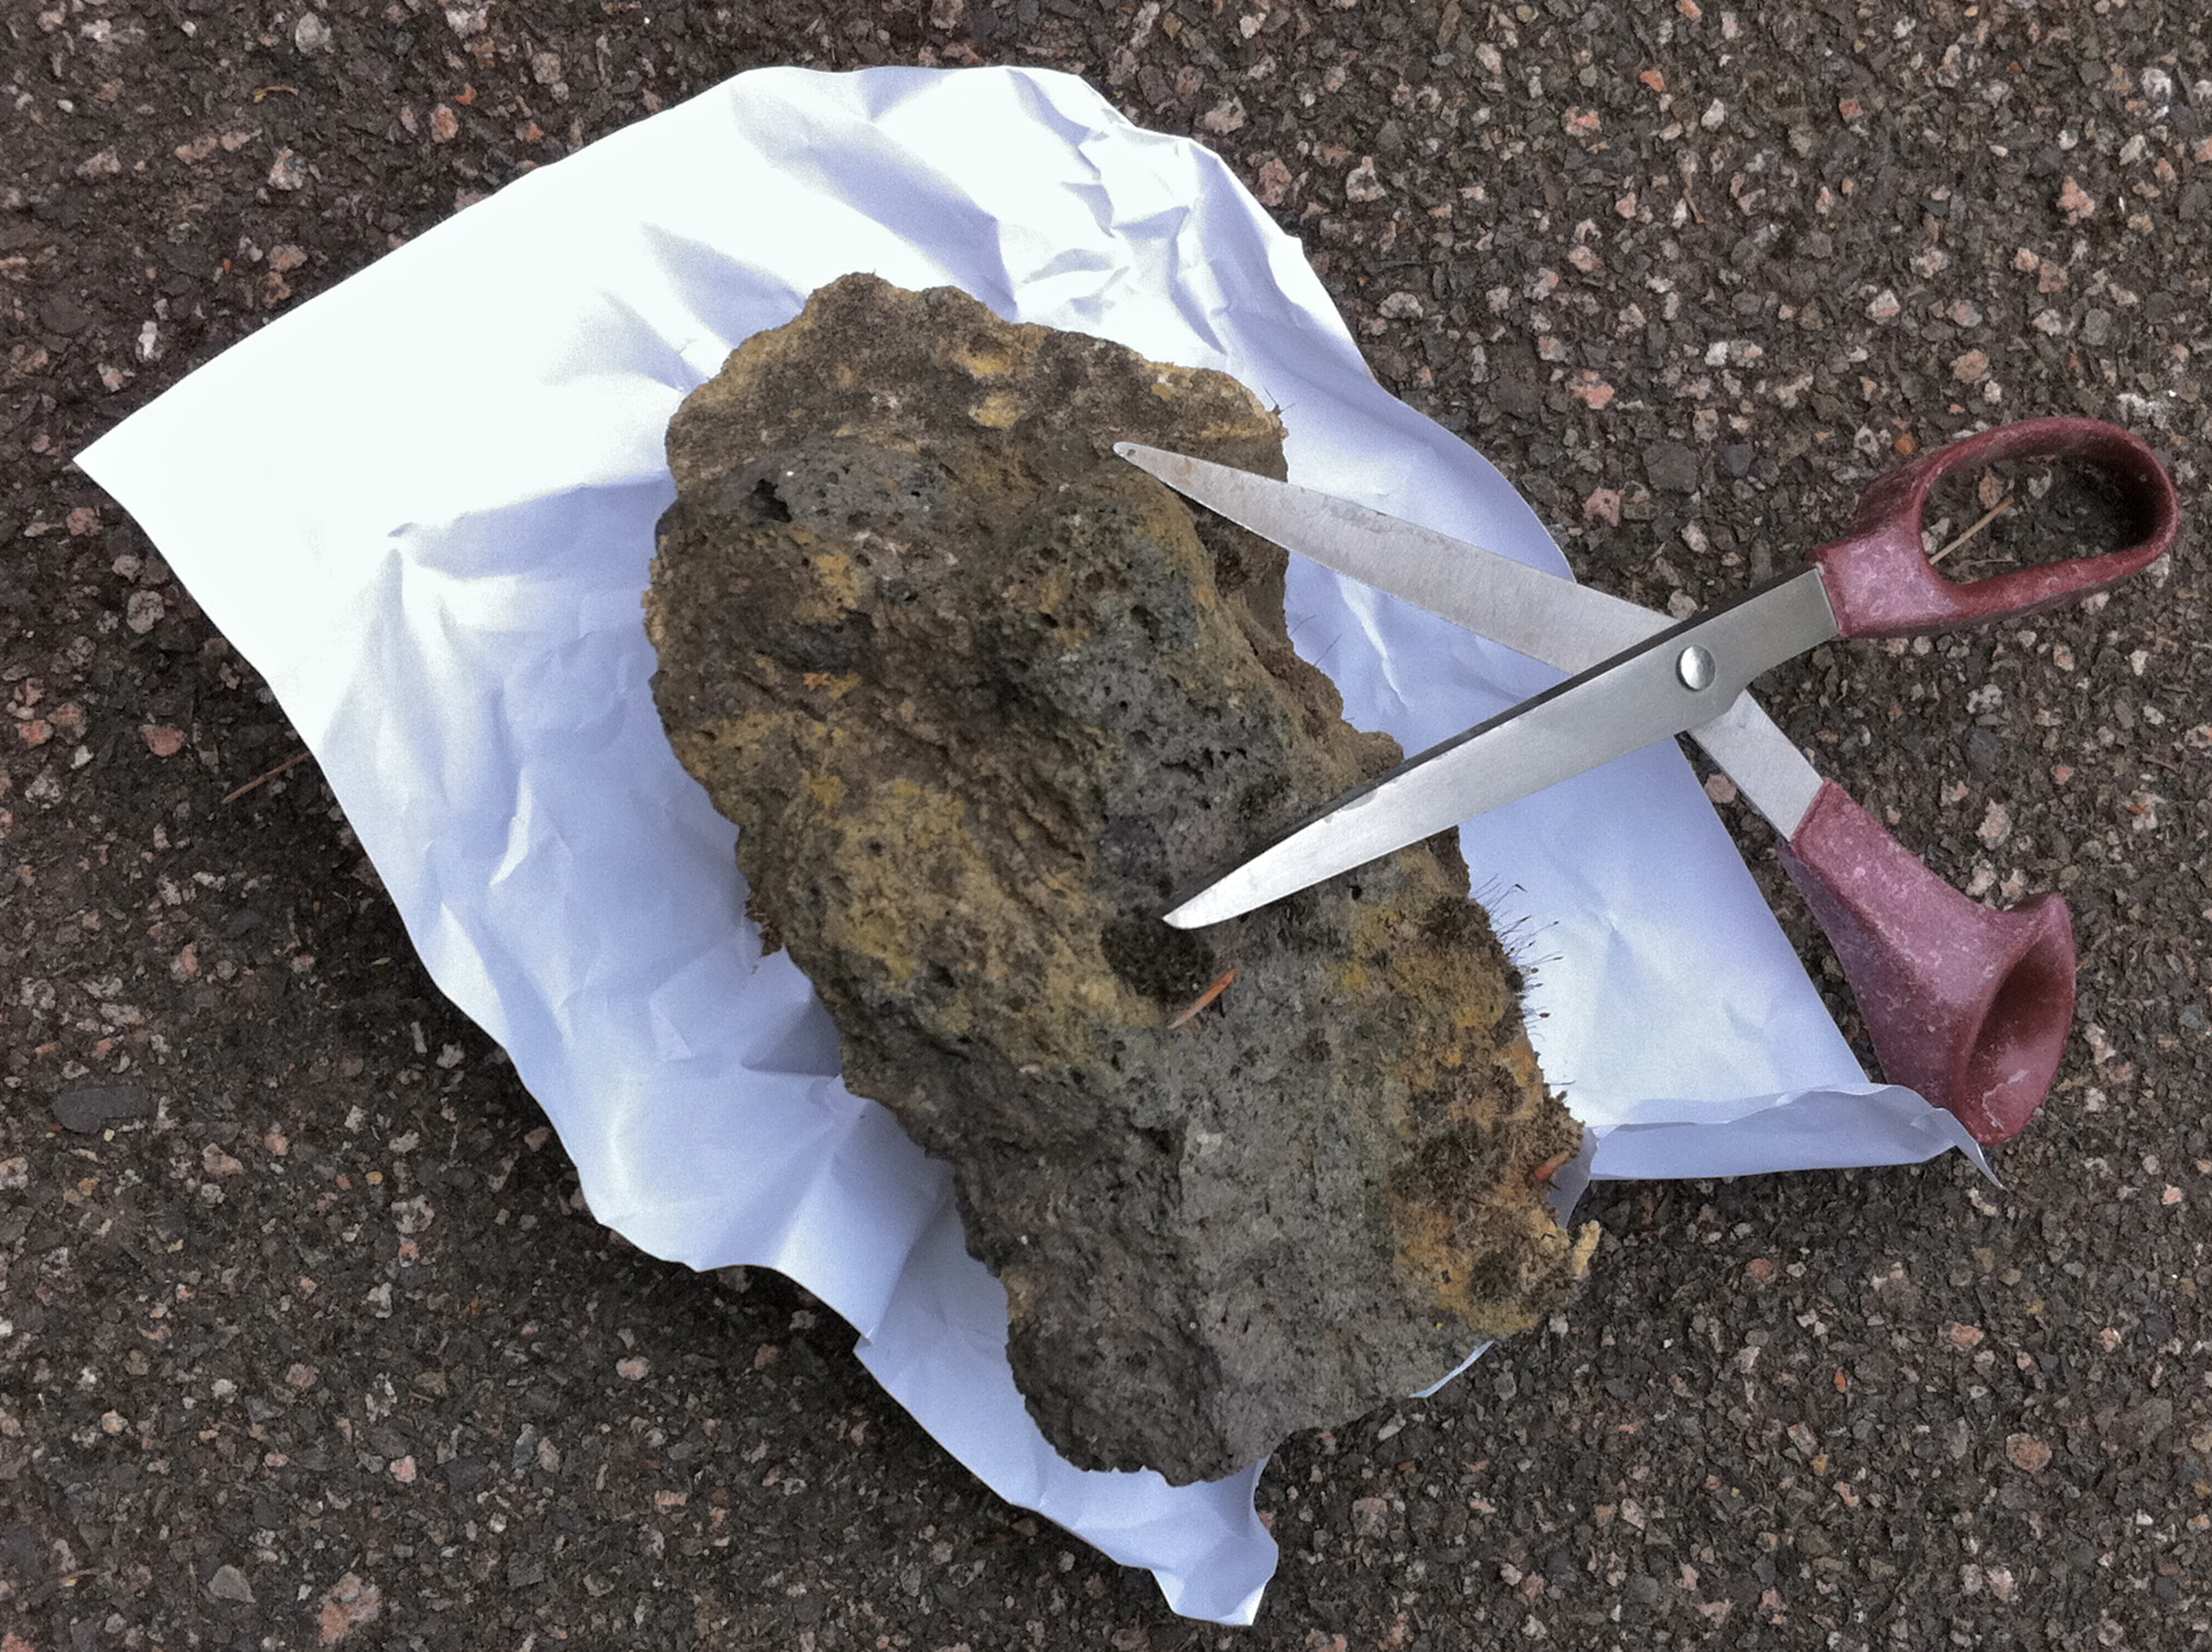
\includegraphics[width=5cm]{Pictures/RPS.pdf}
\end{wrapfigure}
Two players choose one of Rock, Paper and Scissors after counting to three and making one of these gestures:
\begin{itemize}
\item
\textbf{A clenched fist} which represents a rock.
\item
\textbf{A flat hand} representing a piece of paper.
\item
\textbf{Index and middle figure extended} which represents a pair of scissors.
\end{itemize}

\noindent
If they choose the same gesture, neither wins; if not, the result is decided this way:

\begin{itemize}
\item Rock defeats scissors, because a rock will blunt a pair of scissors.
\item Paper defeats rock, because a paper can wrap up a rock.
\item Scissors defeat paper, because scissors cut paper.
\end{itemize}
Suppose that we want to model this in Haskell. One option would be to use integers, characters or strings (which we'll find out about later), but none of these is ideal, for a number of reasons.
\begin{itemize}
\item
A choice may well be arbitrary: what numbers should we associate with `rock', which with `scissors'?
\item
The type we would choose would have lots of other elements which don't correspond to anything in the game.
\end{itemize} 
So, instead, we will define a \texttt{data} type with three members  
\begin{alltt}\minx{Move}
data Move = Rock | Paper | Scissors
\end{alltt}
where we list the members separated by a vertical bar. We can also put the different members on different lines, like this:
\begin{alltt}
data Move = Rock | 
            Paper | 
            Scissors
\end{alltt}
Whatever the case, we add another line -- some `Haskell magic' which we'll explain in Chapter \ref{typeClasses} -- which allows us to compare elements of this type for equality, and also to be able to see them printed out (or `shown'), like so:
\begin{alltt}\minx{deriving}
data Move = Rock | Paper | Scissors
            deriving (Show,Eq)
\end{alltt}
Now we can begin to define functions using the \texttt{Move} type.
Let's write a function which tells us the move to \texttt{beat} a particular move:
\begin{alltt}\minx{beat}
beat :: Move -> Move

beat Rock     = Paper
beat Paper    = Scissors
beat Scissors = Rock
\end{alltt}
and also the move that will \texttt{lose} against a particular move.
\begin{alltt}\minx{lose}
lose :: Move -> Move

lose Rock  = Scissors
lose Paper = Rock
lose _     = Paper
\end{alltt}
In the definition of \texttt{lose} we've used a wildcard `\_' instead of \texttt{Scissors} in the final clause of the definition. That is because this clause is only matched when the others don't, and that will only happen for the value \texttt{Scissors}.

We will come back to this example in Section \ref{strategiesRPS} once we have covered lists in Haskell, when we'll 
look at some of the strategies for playing (and winning!) Rock - Paper - Scissors.


\begin{exercises}

\item
Define a \texttt{data} type \texttt{Result} which represents the outcome of a round of rock - paper - scissors, which will either be a win. lose or draw.

\item
Define a function
\begin{alltt}
outcome :: Move -> Move -> Result
\end{alltt}
so that this gives the outcome of a round for the first player. For example, we should expect that \texttt{outcome Rock Scissors} should be a win.

\item
We have added some `magic' to the \texttt{Chapter4} module to allow QuickCheck properties to be tested over the \texttt{Move} type. Define a QuickCheck property which connects the results of \texttt{beat} and \texttt{lose}.

\item
How would you define a QuickCheck property to test the \texttt{outcome} function?

\end{exercises}

\subsection*{Standard types}

We can see some standard types as being defined in this way. In particular, we could define \texttt{Bool} like this:
\begin{alltt}\minx{Bool}
data Bool = False | True
            deriving (Show, Eq, Ord)
\end{alltt}
Deriving \texttt{Ord} means that the elements have an ordering defined on them; in this case \texttt{False < True}.

\begin{exercises}

\item
Define a type of seasons, \texttt{Season}, and give a function from seasons to temperature given by the type
\begin{alltt}
data Temp = Cold | Hot
            deriving (Eq, Show, Ord)
\end{alltt}
In defining this function assume that you're in the UK.

\item
Define a type \texttt{Month} and a function from this type to \texttt{Season}, assuming that you're in the northern hemisphere.

\end{exercises}

\index{Rock - Paper - Scissors|)}
\index{enumerated type|)}\index{type!enumerated|)}

\section{Recursion}
\label{recursionIntro}
\index{recursion|(}

Recursion is an important programming mechanism, in which a definition of
a function or other object refers to the object itself. This section
concentrates on explaining the idea of recursion, and why it makes
sense.
In particular we give two complementary explanations
of how primitive recursion works in defining the factorial function over the
natural numbers. In the section after this we look at how recursion is
{\em used\/} in practice.

\subsection*{Getting started: a story about factorials}
\index{factorial|(}
\index{recursion!justification|(}

Suppose that someone tells us that the factorial of a natural number is
the product of all natural numbers from one up to (and including) that number, so
that, for instance
\begin{alltt}
fac 6 = 1*2*3*4*5*6
\end{alltt}
Suppose we are also asked to write down a table of factorials, 
where we take the factorial of zero to be
one. We begin thus
\begin{alltt}
  n      fac n
  0        1
  1        1 
  2        1*2 = 2
  3        1*2*3 = 6
  4        1*2*3*4 = 24
\end{alltt}
but we notice that we are repeating a lot of multiplication in doing
this. In working out
\begin{alltt}
1*2*3*4
\end{alltt} we see that we are repeating the
multiplication of \texttt{1*2*3} before multiplying the result by
\texttt{4}
\begin{alltt}
\framebox{1*2*3}\hspace{3pt}*4
\end{alltt}
and this suggests that we can produce the table in a different way, by
saying how to start
\begin{alltt}
fac 0 = 1\hfill(fac.1)
\end{alltt}
which starts the table thus
\begin{alltt}
  n      fac n
  0        1
\end{alltt}
and then by saying how to go from one line to the next
\begin{alltt}
fac n = fac (n-1) * n\hfill(fac.2)
\end{alltt}
since this gives us the lines
\begin{alltt}
  n      fac n
  0        1
  1        1*1 = 1
  2        1*2 = 2
  3        2*3 = 6
  4        6*4 = 24
\end{alltt}
and so on.

What is the moral of this story? We started off describing the table in
one way, but came to see that all we needed was the information in
\texttt{(fac.1)} and \texttt{(fac.2)}.
\begin{itemize}
\item \texttt{(fac.1)} tells us the first line of the table, and
\item \texttt{(fac.2)} tells us how to get from one line of the table to
the next.
\end{itemize}
The table is just a written form of the factorial function, so we can
see that
\texttt{(fac.1)} and \texttt{(fac.2)}
actually describe the \textbf{function} to calculate the factorial, and
putting them together we get
\begin{alltt}\minx{fac}
fac :: Integer -> Integer
fac n
  | n==0        = 1
  | n>0         = fac (n-1) * n
\end{alltt}
A definition like this is called \textbf{recursive} because we actually
use \texttt{fac} in describing \texttt{fac}
itself. Put this way it may sound paradoxical: after all,
how can we describe something in
terms of itself? But, the story we have just told shows that the definition
is perfectly sensible, since it gives
\begin{itemize}
\item a starting point: the value of \texttt{fac} at \texttt{0}, and
\item a way of going from the value of \texttt{fac} at a particular
point, \texttt{fac (n-1)}, to the value of \texttt{fac} on the next
line, namely \texttt{fac n}.
\end{itemize}
These recursive rules will give a value to \texttt{fac n} whatever the
(positive) value \texttt{n}
has -- we just have to write out \texttt{n}
lines of the table, as it were.


\subsection*{Recursion and calculation}
\index{calculation!and recursion}
\index{recursion!and calculation}

The story in the previous section described how the definition of factorial
\begin{alltt}
fac :: Integer -> Integer
fac n
  | n==0        = 1\hfill(fac.1)
  | n>0         = fac (n-1) * n\hfill(fac.2)
\end{alltt}
can be seen as generating the table of factorials, starting from \texttt{fac
0} and working up to \texttt{fac 1}, \texttt{fac 2} and so forth, up to
any value we wish.

We can also read the definition in a calculational way, and see
recursion justified in another way. Take the example of \texttt{fac 4}
\begin{alltt}
fac 4
\step fac 3 * 4
\end{alltt}
so that \texttt{(fac.2)} replaces one goal -- \texttt{fac 4} -- with a
simpler goal -- finding \texttt{fac 3} (and multiplying it by
\texttt{4}). Continuing to use \texttt{(fac.2)}, we have
\begin{alltt}
fac 4
\step fac 3 * 4
\step (fac 2 * 3) * 4
\step ((fac 1 * 2) * 3) * 4
\step (((fac 0 * 1) * 2) * 3) * 4
\end{alltt}
Now, we have got down to the simplest case (or \textbf{base case}),
\index{recursion!base case}
which is solved by \texttt{(fac.1)}.
\begin{alltt}
\step (((1 * 1) * 2) * 3) * 4
\step ((1 * 2) * 3) * 4
\step (2 * 3) * 4
\step 6 * 4
\step 24
\end{alltt}
In the calculation we have worked from the goal back down to the base
case, using the \textbf{recursion step}
\index{recursion!recursion step}
 \texttt{(fac.2)}. We can again
see that we get the result we want, because the recursion step takes us
from a more complicated case to a simpler one, and we have given a value
for the simplest case (zero, here) which we will eventually reach.

We have now seen in the case of \texttt{fac} two explanations for why
recursion works. 
\begin{itemize}
\item\index{recursion!bottom-up}
The \textbf{bottom-up} explanation says that the \texttt{fac} equations can be 
seen to generate the
values of \texttt{fac} one-by-one from the base case at zero. 
\item\index{recursion!top-down}
A \textbf{top-down} view starts with a goal to be evaluated, and shows how
the equations simplify this until we hit the base case.
\end{itemize}
The two views here are related, since we can think of the top-down
explanation generating a table too, but in this case the table is
generated as it is needed. Starting with the goal of \texttt{fac 4} we
require the lines for \texttt{0} to \texttt{3} also.

Technically, we call the form of recursion we have seen here
\textbf{primitive recursion}.\index{recursion!primitive}
\index{primitive recursion} We will describe it more formally in the
next section, where we examine how to start to find recursive
definitions. Before we do that, we discuss another aspect of the
\texttt{fac} function as defined here.
\index{factorial|)}
\index{recursion!justification|)}

\subsection*{Undefined or error values}
\index{undefinedness}
\index{value!undefined}
\index{value!error}

Our definition of factorial covers zero and the positive integers. What
will be the effect of applying \texttt{fac}
to a negative number? On evaluating \texttt{fac (-2)} in GHCi we receive
the error message
\begin{alltt}
*** Exception: Chapter4.hs:(106,0)-(108,33): 
        Non-exhaustive patterns in function fac
\end{alltt}
because \texttt{fac} is not defined on the negative numbers, since the patterns in the definition of \texttt{fac} don't cover the case of negative numbers.

We could if
we wished extend the definition to zero, on the negative numbers, thus
\begin{alltt}
fac n
  | n==0        = 1
  | n>0         = fac (n-1) * n
  | otherwise   = 0
\end{alltt}
or we could include our own error message, as follows
\begin{alltt}
fac n
  | n==0        = 1
  | n>0         = fac (n-1) * n
  | otherwise   = error "fac only defined on natural numbers"\minx{error}
\end{alltt}
so that when we evaluate \texttt{fac (-2)} we receive the message
\begin{alltt}
Program error: fac only defined on natural numbers
\end{alltt}
The error message here is a Haskell string, as discussed in Chapter
5.

\begin{exercises}

\item Define the function \texttt{rangeProduct}
which when given natural numbers \texttt{m} and
\texttt{n} returns the product 
\begin{alltt}
m*(m+1)*...*(n-1)*n
\end{alltt}
You should include in your definition the type of the function, and your function
should return \texttt{0} when \texttt{n} is smaller than \texttt{m}.\\
{Hint:} you do
not need to use recursion in your definition, but you may if you wish.

\item As \texttt{fac} is a special case of \texttt{rangeProduct}, 
write a definition of \texttt{fac}
which {\em uses\/} \texttt{rangeProduct}.
\end{exercises}

\section{Primitive recursion in practice}

This section examines how primitive recursion is used in practice by
examining a number of examples.

The pattern of primitive recursion says that we can define a function
from the natural numbers \texttt{0}, \texttt{1}, \ldots by giving the
value at zero, and by explaining how to go from the value at
\texttt{n-1} to the value at \texttt{n}. We can give a \textbf{template} for this
\begin{alltt}\index{primitive recursion!template}
fun n
  | n==0        = ....\hfill(prim)
  | n>0         = .... fun (n-1) ....
\end{alltt}
where we have to supply the two right-hand sides.

How can we decide whether a function can be defined in this way? Just as we did
earlier in the chapter, we frame a question which summarizes the
essential property we need for 
primitive recursion to apply.

\subsubsection*{{\bfseries What if\/} we were given the value 
{\tt fun} {\tt (n-1)}. How could we define {\tt fun} {\tt n\/} from it?}

We see how this form of recursion works in practice by looking at some examples.
\index{primitive recursion!examples on numbers}

\begin{example} 
\noindent{\sf 1.}\hskip1em Suppose first that we are asked to
define the function to give us powers of two for natural numbers
\begin{alltt}
power2 :: Integer -> Integer
\end{alltt}
so that \texttt{power2 n} is \superscr{2}{n}, that is \texttt{2}
multiplied by itself \texttt{n} times.
The template is
\begin{alltt}
power2 n
  | n==0        = ....
  | n>0         = .... power2 (n-1) ....
\end{alltt}
In the zero case the result is \texttt{1}, and in general
\superscr{2}{n} is
\superscr{2}{n-1} multiplied by 2, so we define
\begin{alltt}\minx{power2}
power2 n
  | n==0        = 1
  | n>0         = 2 * power2 (n-1)
\end{alltt}

\subexample*{2.}As the next example we take the function
\begin{alltt}\minx{sumFacs}
sumFacs :: Integer -> Integer
\end{alltt}
so that
\begin{alltt}
sumFacs n = fac 0 + fac 1 + ... + fac (n-1) + fac n
\end{alltt}
If we are told that \texttt{sumFacs 4} is \texttt{34} then we can work
out \texttt{sumFacs 5} in one step: we simply add \texttt{fac 5}, that
is \texttt{120}, giving the result \texttt{154}. This works in general, and so 
we can fill in the
template like this:
\begin{alltt}\minx{sumFacs}
sumFacs :: Integer -> Integer
sumFacs n
  | n==0        = 1
  | n>0         = sumFacs (n-1) + fac n  
\end{alltt}
In fact this pattern works for any function \texttt{f} of type 
\texttt{Integer -> Integer} in the place of \texttt{fac}, so
we can say
\begin{alltt}\minx{sumFun}
sumFun :: (Integer -> Integer) -> Integer -> Integer
sumFun f n
  | n==0        = f 0
  | n>0         = sumFun f (n-1) + f n  
\end{alltt}
where the function whose values are being added is itself an argument of the 
\texttt{sumFun}
function.
A sample calculation using \texttt{sumFun} is
\begin{alltt}
sumFun fac 3
\step sumFun fac 2 + fac 3
\step sumFun fac 1 + fac 2 + fac 3
\step sumFun fac 0 + fac 1 + fac 2 + fac 3
\step fac 0 + fac 1 + fac 2 + fac 3
\step ...
\step 10
\end{alltt}
and we can define \texttt{sumFacs} from \texttt{sumFun} thus:
\begin{alltt}
sumFacs n = sumFun fac n
\end{alltt}

We briefly introduced the idea of functions as data
in Chapter \ref{intro}, and we will revisit it in detail in 
Chapter \ref{patternsGen}. As we mentioned in Chapter \ref{intro}, having functions as
arguments is powerful  and \texttt{sumFun}
gives a good example: one definition serves to sum the values of {\em any\/} function 
of type  \texttt{Integer -> Integer} over the range of arguments from \texttt{0} to \texttt{n}. 

\subexample*{3.}As a last example we look at a geometrical
problem. Suppose we want to find out the maximum number of
pieces we can get by making a given number of straight-line
cuts  across a piece of paper. With no cuts we get one piece;
what about the general case? Suppose we have \texttt{n-1} lines
already, and that we add one more. 
\begin{center}
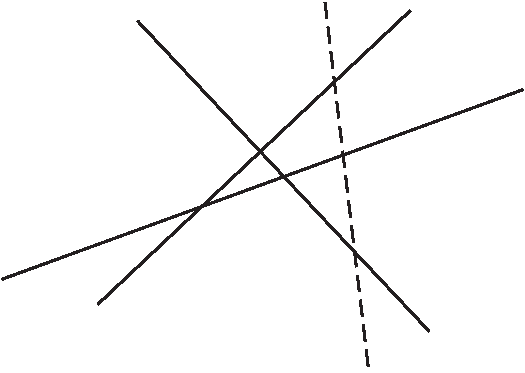
\includegraphics{Pictures/cuts.pdf}
\end{center}
We will get the most new
regions if we cross each of these lines; because they are straight
lines, we can only cut each one once. This means that the new line
crosses exactly \texttt{n} of the regions, and so splits each of these
into two. We therefore get \texttt{n} new regions by adding the
\texttt{n}th line. Our function definition is given by filling in the template 
\texttt{(prim)} according to what we have said.
\begin{alltt}\minx{regions}
regions :: Integer -> Integer 
regions n
  | n==0        = 1
  | n>0         = regions (n-1) + n
\end{alltt}
\end{example}

\begin{exercises}

\item Using the addition function over the natural numbers, give a recursive definition 
of multiplication of natural numbers.

\item The integer square root of a positive integer \texttt{n} is the largest
integer whose square is less than or equal to \texttt{n}. For instance,
the integer square roots of \texttt{15}
and \texttt{16} are \texttt{3} and \texttt{4}, respectively. Give a
primitive recursive definition of this function.

\item Given a function \texttt{f} of type \texttt{Integer -> Integer} give a
recursive definition of a function of type \texttt{Integer -> Integer}
which on input \texttt{n} returns the 
maximum of the values \texttt{f 0}, \texttt{f 1}, \ldots, \texttt{f n}. You
might find the \texttt{max} function defined in Section \ref{guards} useful.

To test this function, add to your script a definition of some values of
\texttt{f} thus:
\begin{alltt}
f 0 = 0
f 1 = 44
f 2 = 17
f _ = 0
\end{alltt}
and so on; then test your function at various values.

\item Given a function \texttt{f} of type \texttt{Integer -> Integer} give a
recursive definition of a function of type \texttt{Integer -> Bool}
which on input \texttt{n} returns \texttt{True} if one or more of the values
\texttt{f 0}, \texttt{f 1}, \ldots, \texttt{f n} is zero and
\texttt{False} otherwise.

\item
Can you give a definition of \texttt{regions}
which instead of being recursive {\em uses\/} the function \texttt{sumFun}?

\item 
{[Harder]} Find
out the maximum number of pieces we can get
by making a given number of flat (that is planar) cuts 
through a solid block. It is {\em not\/} the same answer as we calculated
for straight-line cuts of a flat piece of paper. 
\end{exercises}


\section{Extended exercise: pictures}
\index{pictures!extended exercise|(}

This section looks at how recursion over integers can be used to describe geometrical patterns, using pictures as implemented in \texttt{PicturesSVG} (or \texttt{Pictures}).
We start by giving a definition of a line of \texttt{n} black squares:
\begin{alltt}
blackSquares :: Integer -> Picture

blackSquares n
  | n<=1	     = black
  | otherwise = black `beside` blackSquares (n-1)
\end{alltt}
or diagrammatically,
\begin{center}

\includegraphics[width=2.5in]{Pictures/blackSquares.pdf}
\end{center}
Suppose that we want to build a line of alternating black and white squares: we get this by putting a black square on the front of a line beginning with a white square:
\begin{alltt}
blackWhite :: Integer -> Picture

blackWhite n
  | n<=1	     = black
  | otherwise = black `beside` whiteBlack (n-1)
\end{alltt}
where \texttt{whiteBlack} is the function that builds a line of alternating squares, beginning with a white. Diagrammatically this is given by
\begin{center}
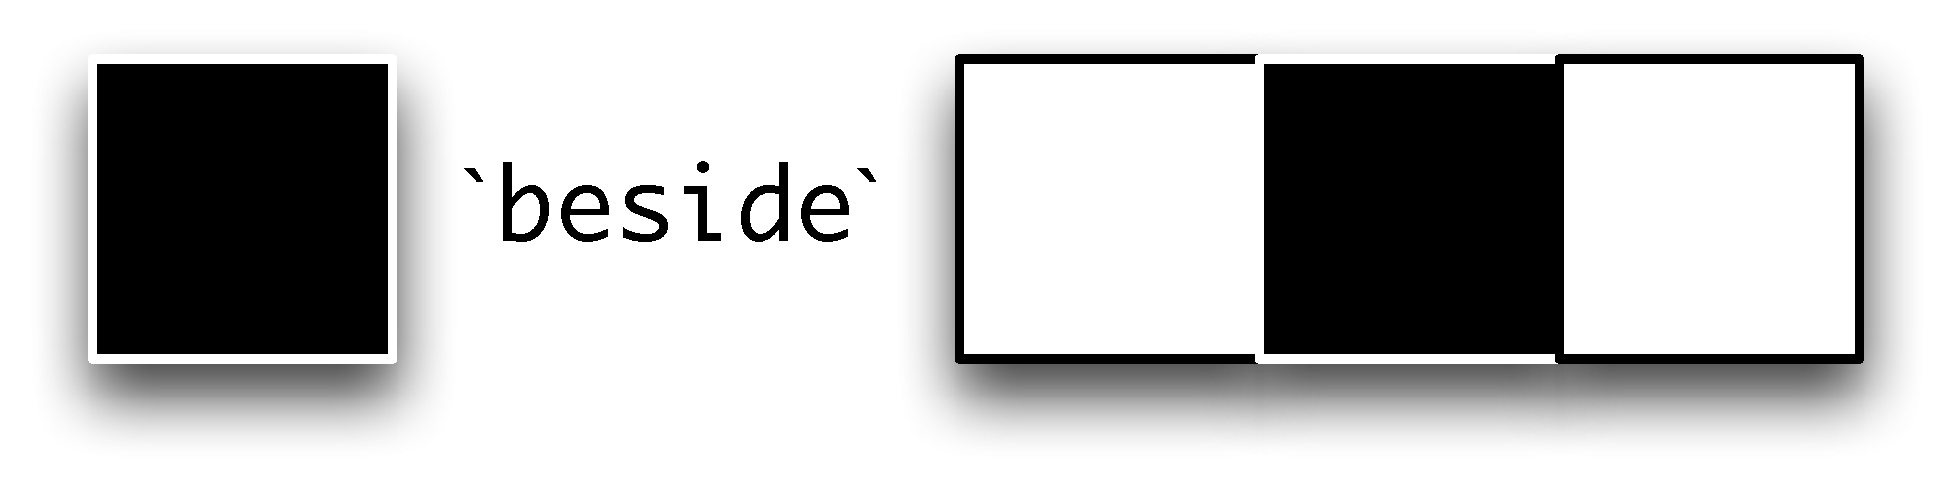
\includegraphics[width=2.5in]{Pictures/blackWhite.pdf}
\end{center}
Using these functions we can build chessboards of any shape:
\begin{alltt}
blackChess :: Integer -> Integer -> Picture

blackChess n m
  | n<=1	     = blackWhite m
  | otherwise = blackWhite m `above` whiteChess (n-1) m
\end{alltt}
where the corresponding function \texttt{whiteChess} builds a board with a white square in the top left-hand corner. Diagrammatically,
\begin{center}
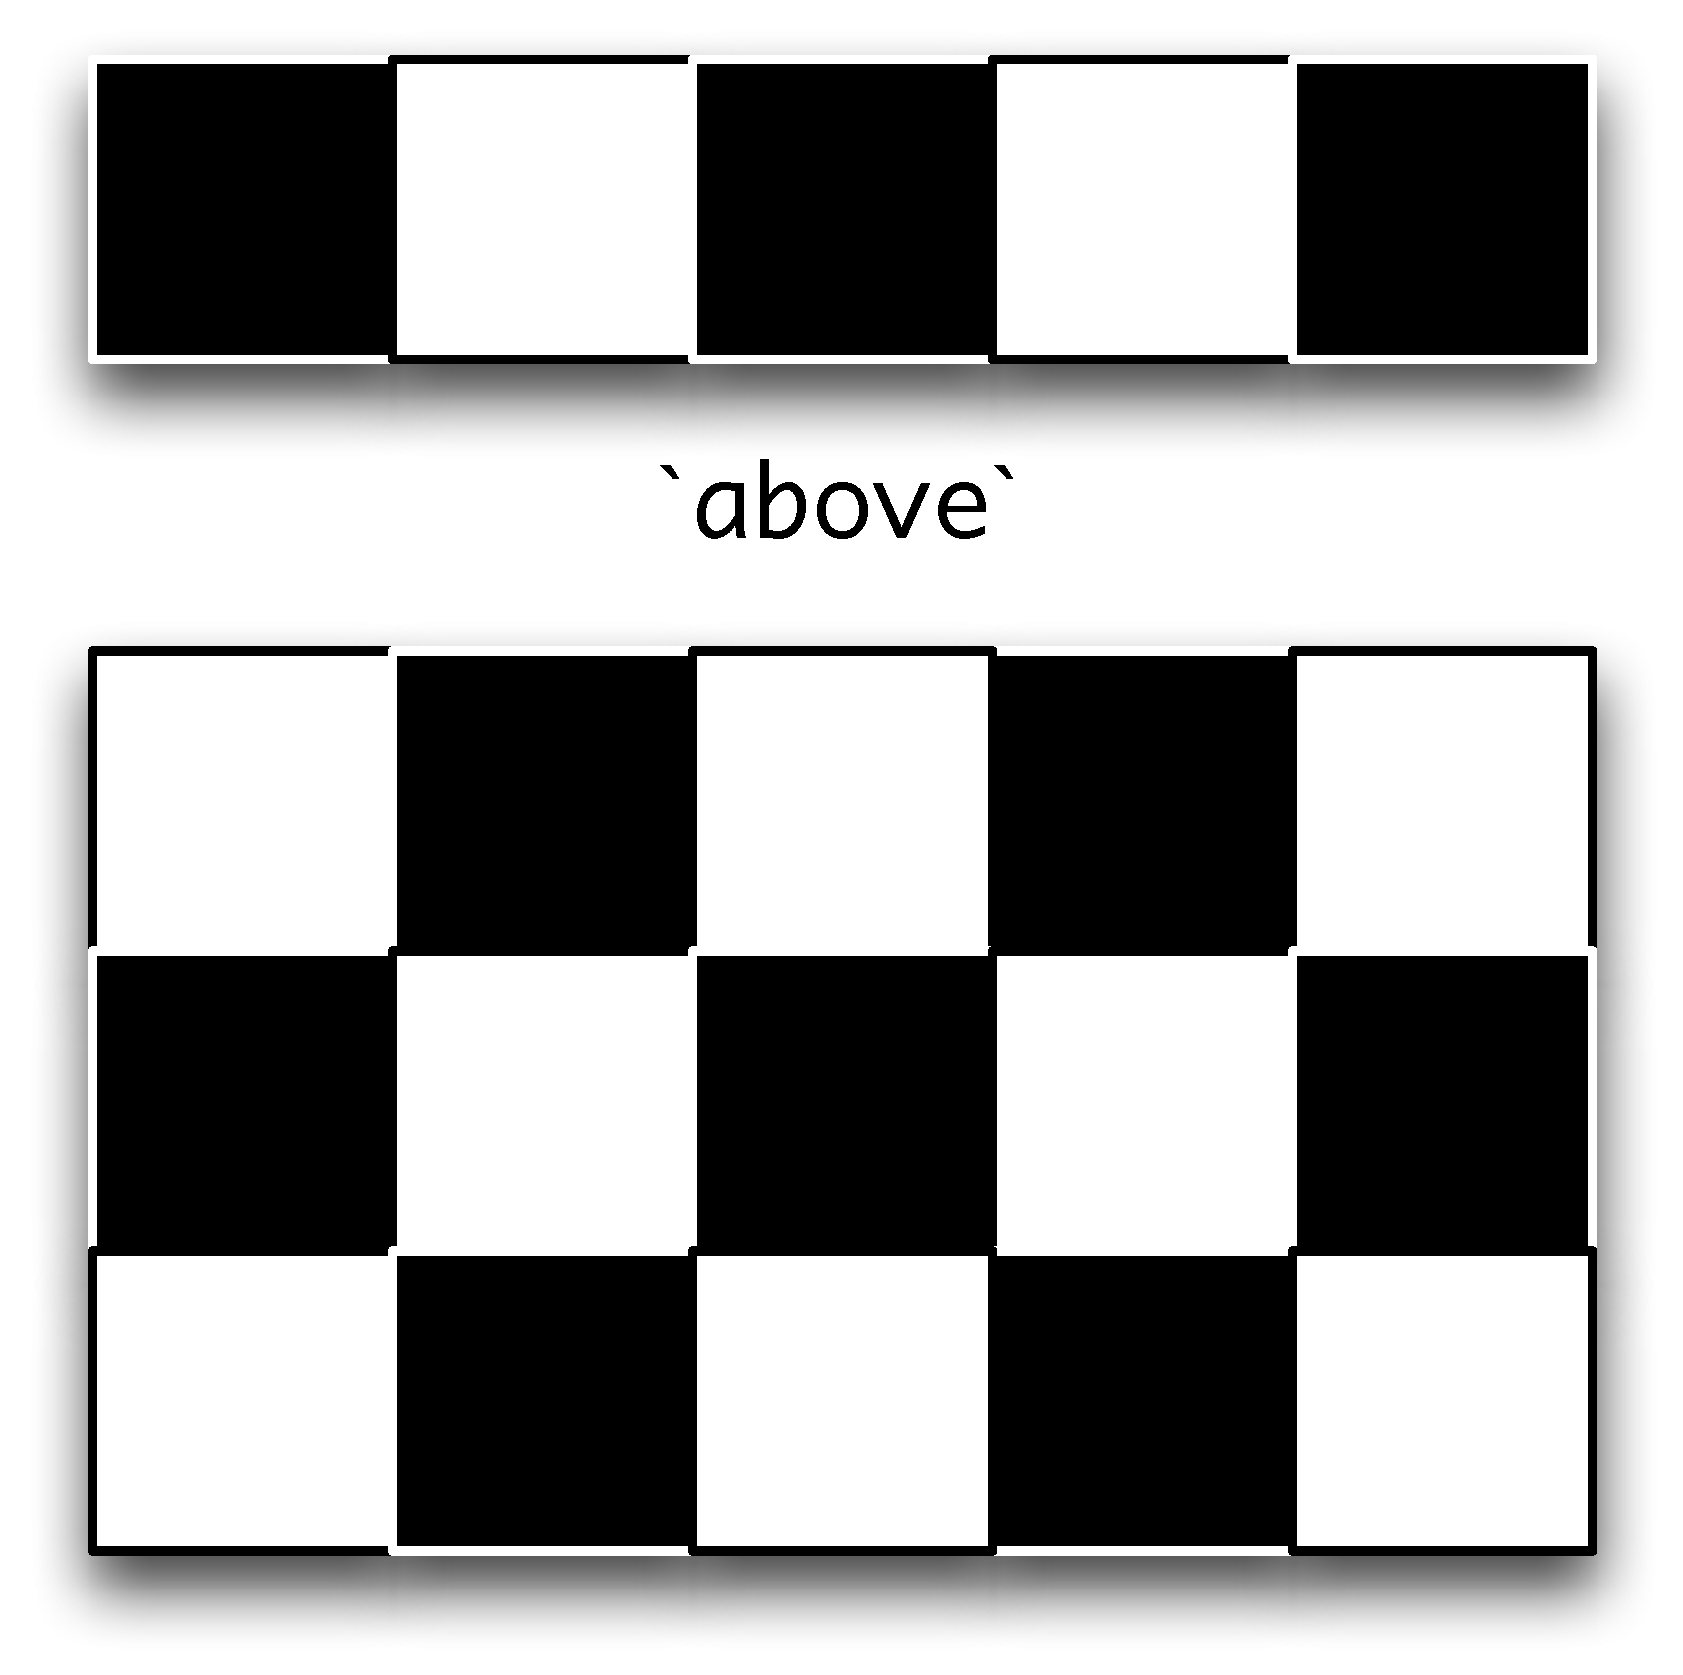
\includegraphics[width=2.5in]{Pictures/chess4.pdf}
\end{center}

\begin{wrapfigure}[8]{r}{1cm}
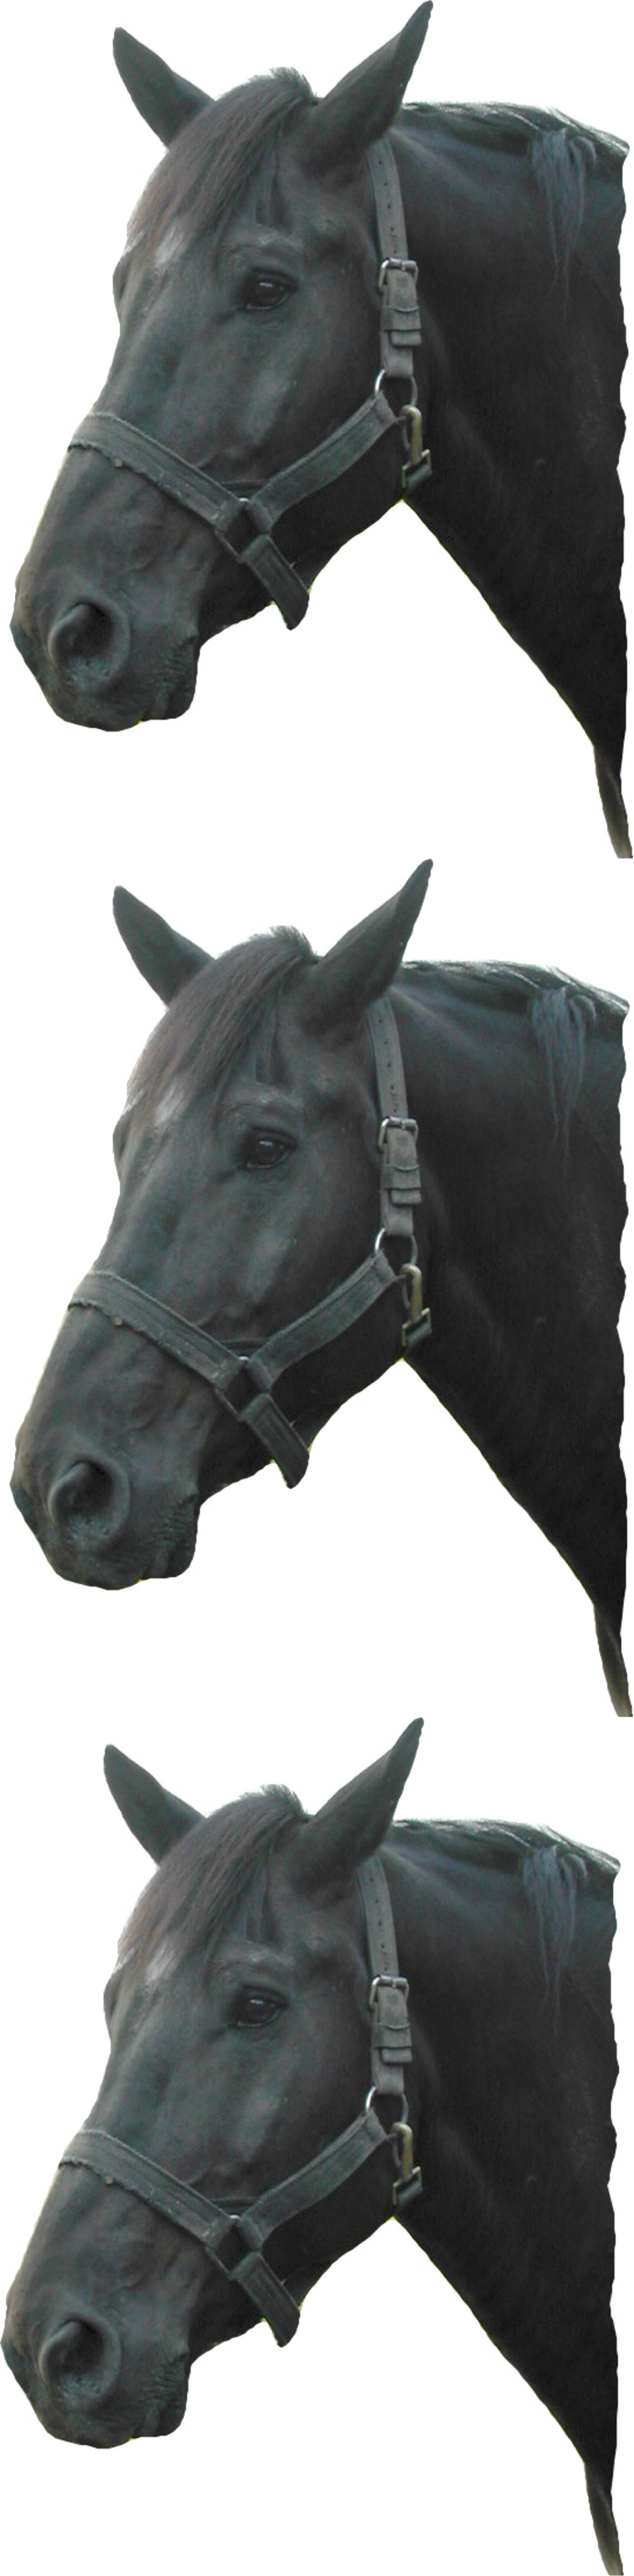
\includegraphics[width=1cm]{Pictures/threeHorses.pdf}
\end{wrapfigure}

\begin{exercises}

\item
Complete the definitions of \texttt{whiteBlack} and \texttt{whiteChess}.

\item
How would you define a function to give a column of pictures,
\begin{alltt}
column :: Picture -> Integer -> Picture
\end{alltt}
so that the result of \texttt{\ column horse 3\ } is as shown to the right.

\item
Give a Haskell function which takes an integer \texttt{n} and returns an  \texttt{n} by \texttt{n} white square with a diagonal black line from top left to bottom right, as in.
\begin{center}
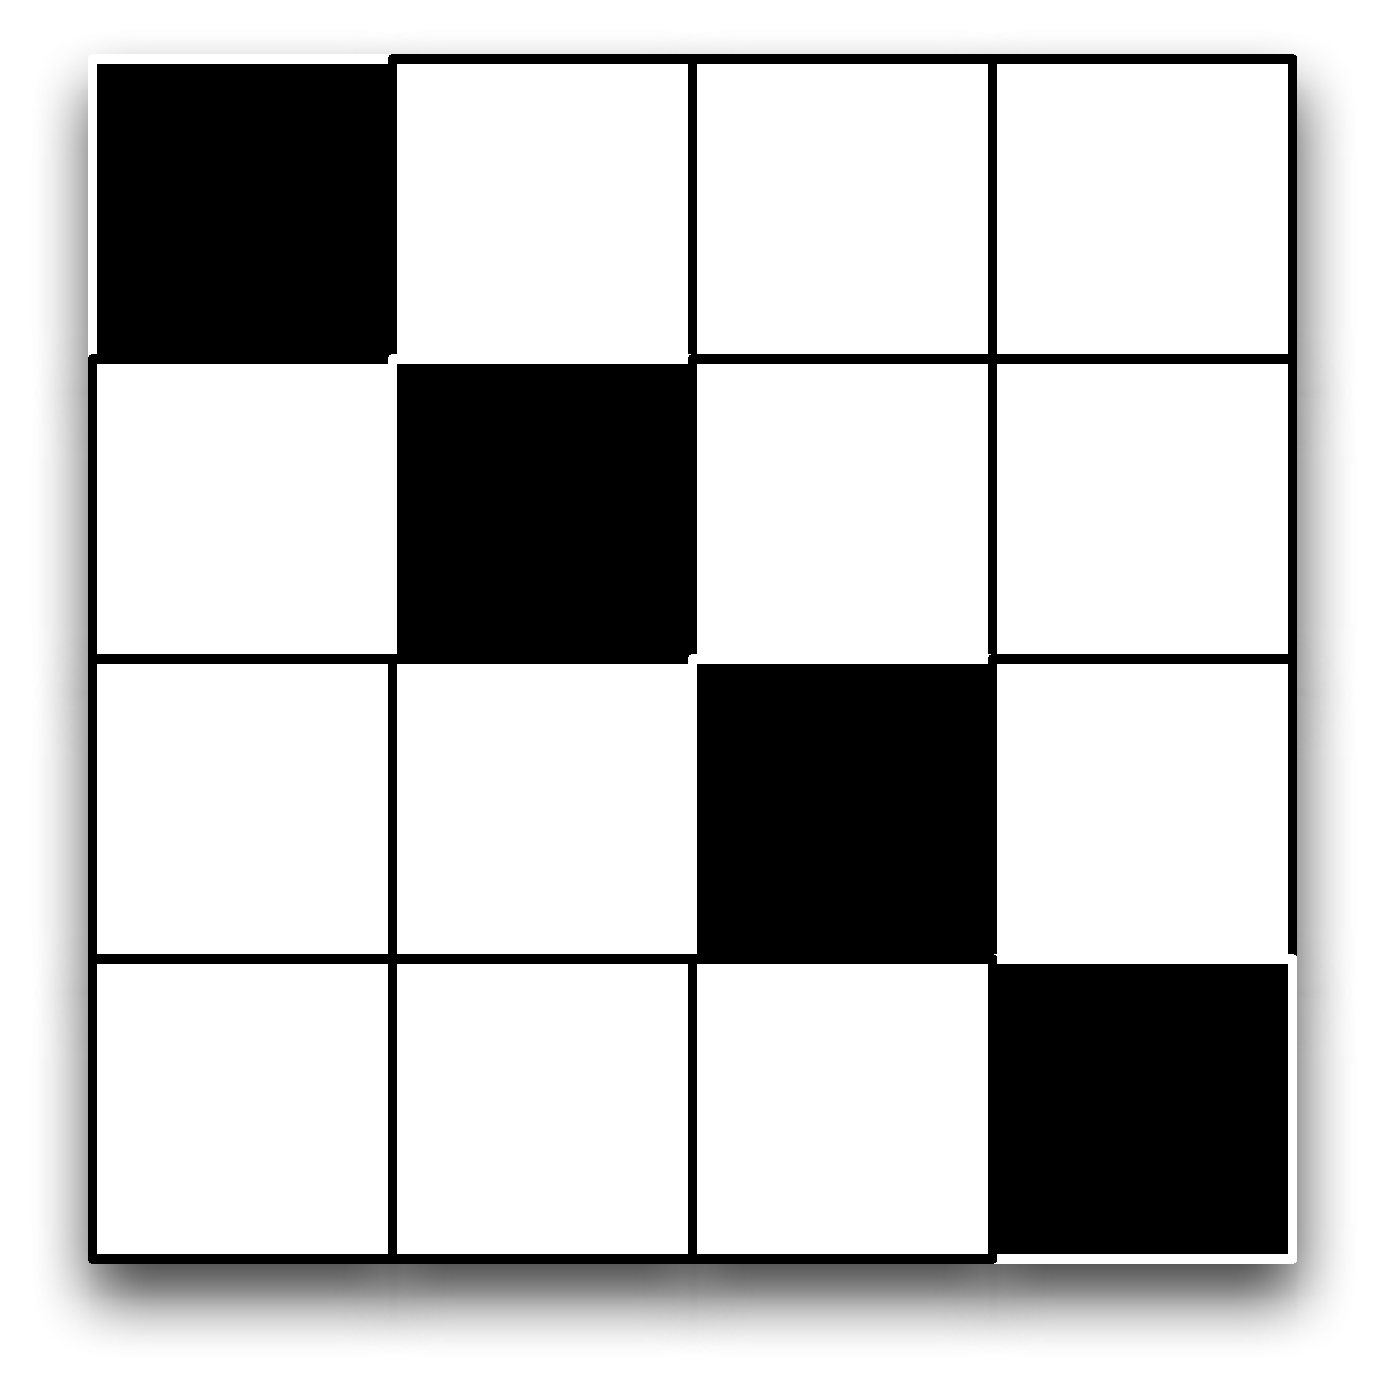
\includegraphics[width=1.5in]{Pictures/diag1.pdf}
\end{center}

\item
Give a Haskell function which takes an integer \texttt{n} and returns an  \texttt{n} by \texttt{n} white square with a diagonal black line from top right to bottom left, as in.
\begin{center}
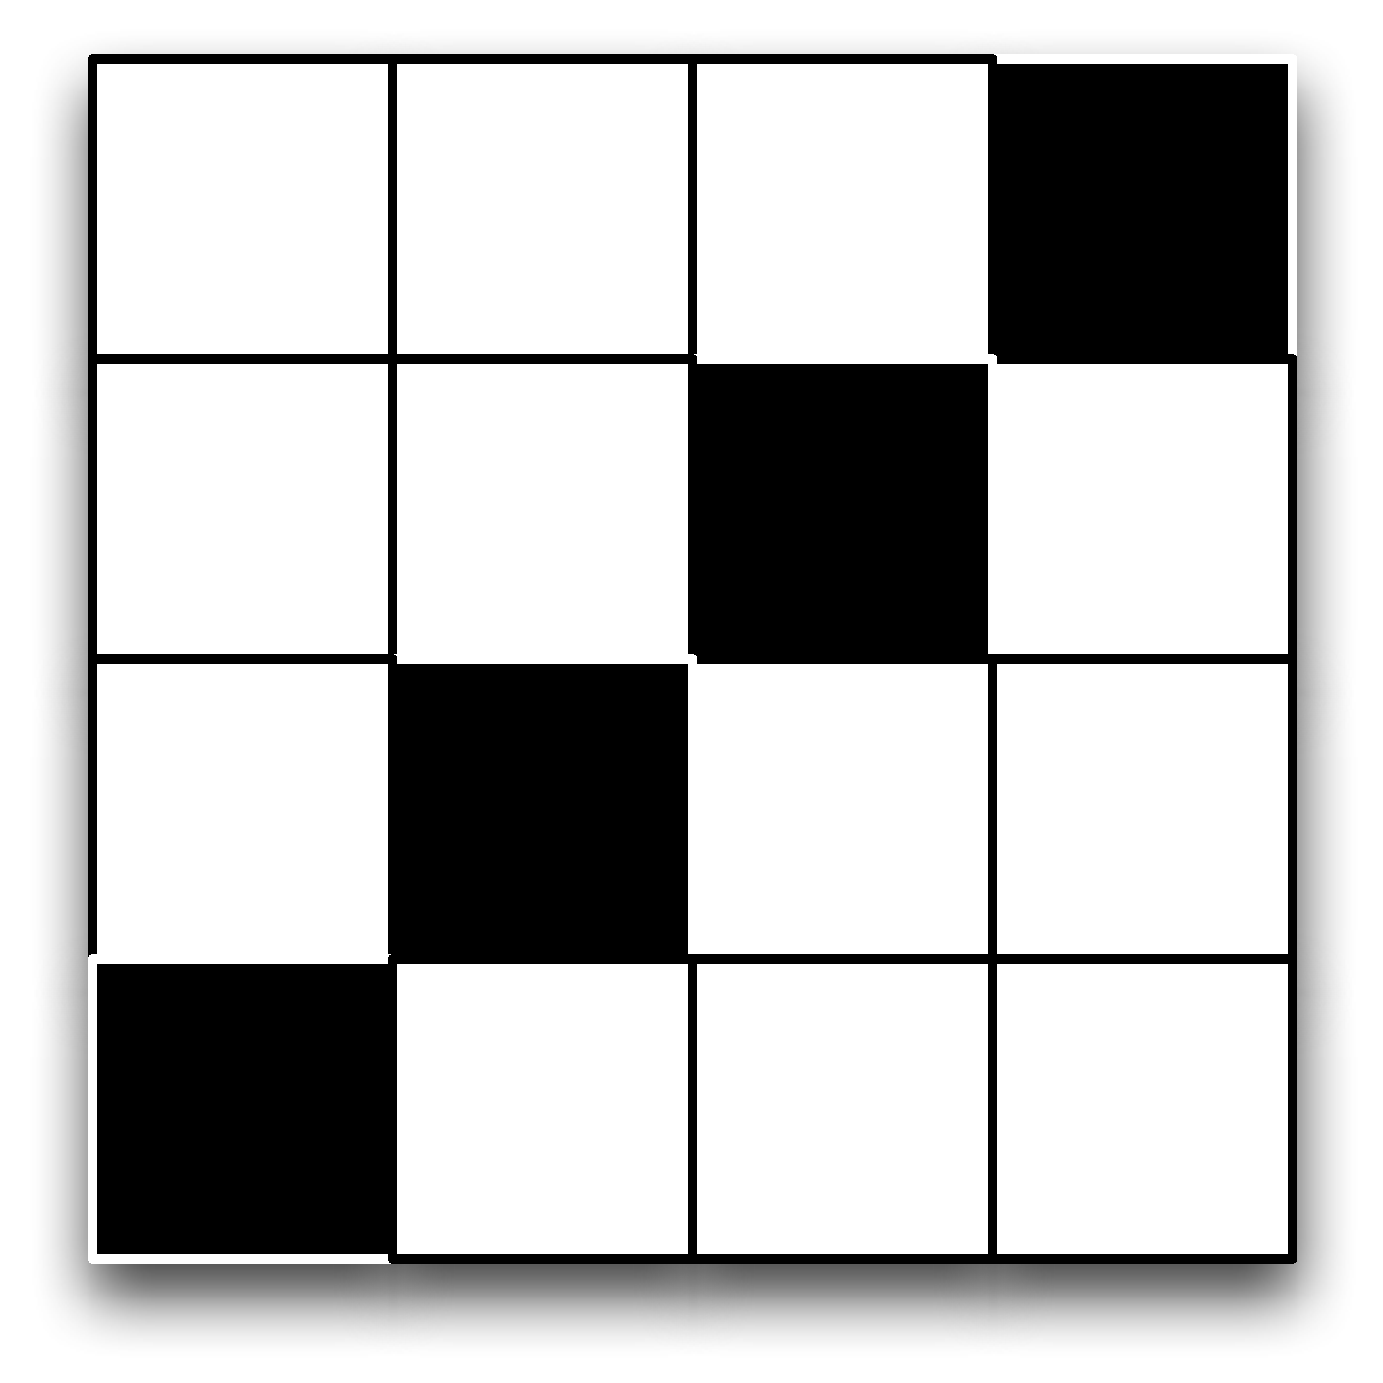
\includegraphics[width=1.5in]{Pictures/diag2.pdf}
\end{center}

\item
Give a Haskell function which takes an integer \texttt{n} and returns an  \texttt{n} by \texttt{n} white square with both diagonals coloured black, as in.
\begin{center}

\includegraphics[width=1.5in]{Pictures/diag3.pdf}
\end{center}

\item
Can you give a direct recursive definition of a  function 
\begin{alltt}
chessBoard :: Integer -> Picture
\end{alltt}
so that 
\begin{alltt}
chessBoard n = ... chessBoard (n-1) ...
\end{alltt}
Hint: you might want to use some of the functions defined here, or variants of them, in writing your definition.

\end{exercises}

\index{pictures!extended exercise|)}



\section{General forms of recursion}
\label{genRecursion}
\index{general recursion|(}
\index{recursion!general|(}

As we explained  in Section \ref{recursionIntro}, a recursive
definition of a function such as \texttt{fac} would give the value of
\texttt{fac n}
using the value \texttt{fac (n-1)}. We saw there that \texttt{fac (n-1)}
is {\em simpler\/} in being closer to the base case \texttt{fac 0}. As
long as we preserve this property of becoming simpler, different patterns
of recursion are possible  and we look at some of them in this section.
These more general forms of recursion are called \textbf{general
recursion}.
In trying to use recursion to define a function we need to pose the
question:

\subsubsection*{In defining {\tt f n} which values of
{\tt f k} would help me to work out the answer?}

\begin{example}
\subexample*{1.}The sequence of Fibonacci numbers starts with
\texttt{0} and
\texttt{1},
\index{Fibonacci numbers}
and subsequent values are given by adding the last two values, so that
we get \texttt{0+1=1}, \texttt{1+1=2} and so forth. This can be given a
recursive definition as follows
\begin{alltt}
fib :: Integer -> Integer
fib n 
  | n==0        = 0
  | n==1        = 1
  | n>1         = fib (n-2) + fib (n-1)
\end{alltt}
where we see in the general case that \texttt{fib n} depends upon not
only \texttt{fib (n-1)} but also \texttt{fib (n-2)}.

This gives a clear description of the Fibonacci numbers, but
unfortunately it gives a very inefficient program for calculating them.
We can see that calculating \texttt{fib n} requires us to calculate both
\texttt{fib (n-2)} and \texttt{fib (n-1)}, and in calculating
\texttt{fib (n-1)} we will have to calculate \texttt{fib (n-2)}
{\em again}. We   look at ways of overcoming this problem in Section 5.2.

\subexample*{2.}Dividing one positive integer by another can be
done in many different ways. One of the simplest ways is
repeatedly to subtract the divisor from the number being
divided,  and we give a program doing that here. In fact we will
define two functions
\begin{alltt}
remainder :: Integer -> Integer -> Integer
divide    :: Integer -> Integer -> Integer
\end{alltt}
which separately give the division's remainder and quotient.

In trying to find a definition it often helps to look at an example.
Suppose we want to divide \texttt{37} by
\texttt{10}. We expect that
\begin{alltt}
remainder 37 10 = 7
divide    37 10 = 3
\end{alltt} 
If we subtract the divisor, \texttt{10}, from the number being divided, \texttt{37}, 
how are the values related?
\begin{alltt}
remainder 27 10 = 7
divide    27 10 = 2
\end{alltt}
The remainder is the same, and the result of the division is one less. 
What happens at the base case? An example is
\begin{alltt}
remainder 7 10 = 7
divide    7 10 = 0
\end{alltt} 
Using these examples as
a guide, we have
\begin{alltt}
remainder m n 
  | m<n         = m
  | otherwise   = remainder (m-n) n
\end{alltt}
\begin{alltt}
divide m n
  | m<n         = 0
  | otherwise   = 1 + divide (m-n) n
\end{alltt}
\end{example}

These definitions also illustrate another important point: a general recursive function
does not always give an answer; instead an evaluation may go on forever. 
Look at what happens if we evaluate
\begin{alltt}
remainder 7 0
\step remainder (7-0) 0
\step remainder 7 0
\step ....
\end{alltt} 
This calculation will loop for ever, and indeed we should expect problems
if we try to divide by zero! However, the problem also appears if we try to divide by a
negative number, for instance
\begin{alltt}
divide 4 (-4)
\step divide (4-(-4)) (-4)
\step divide 8 (-4)
\step ...
\end{alltt}
The lesson of this example is that in general there is no guarantee that a function defined
by recursion will always \textbf{terminate}.\index{termination} 
We will have termination if we use primitive 
recursion, and other cases where we are sure that we always go from a more 
complex case to a simpler one; the problem in the example here is that
subtracting a negative number increases the result, giving a more complex application of the
function.
\index{recursion|)}
\index{general recursion|)}
\index{recursion!general|)}


\begin{exercises}

\item
Give a recursive definition of a function to find the highest common
factor of two positive integers.

\item 
Suppose we have to raise \texttt{2} to the power \texttt{n}. If
\texttt{n} is even, \texttt{2*m} say, then
\begin{alltt}
\superscr{2}{n} = \superscr{2}{2*m} = \superscr{(\superscr{2}{m})}{2}
\end{alltt}
If \texttt{n} is odd, \texttt{2*m+1} say, then
\begin{alltt}
\superscr{2}{n} = \superscr{2}{2*m+1} = \superscr{(\superscr{2}{m})}{2}*2
\end{alltt}
Give a recursive function to compute
\superscr{2}{n} which uses these insights.
\end{exercises}


\section{Program testing}
\label{testing}
\index{testing|(}

Just because a program is accepted by the Haskell system, it does not
mean that it necessarily does what it should.
How can we be sure that a program behaves as it is intended to? One
option, first aired in Section \ref{proof}, is to \textbf{prove} in some way that
it behaves correctly. Proof is, however, an expensive business,
and we can get a good deal of assurance that our programs behave
correctly by testing the program. 

If we are not to use proof, then we can use \textbf{QuickCheck} to test properties of functions using randomly generated data. This has a number of advantages -- we don't have to select input data, for example -- but we do need to define the properties to be tested, and it is not always clear how to do this. So, we can also do traditional testing, where we specify the inputs and expected result for a function.

The art of testing
is then to choose the inputs to be as comprehensive as possible. That is, we
want to test data to represent all the different `kinds' of input that can be
presented to the function.

How might we choose
test data? There are two possible approaches. We could simply be told
the \textbf{specification}\index{specification} of the function, and
devise test data according to that. This is called \textbf{black box}
testing\index{testing!black box}, as we cannot see into the box which
contains the function. On the other hand, in devising \textbf{white box}
\index{testing!white box}tests we can use the form of the function
definition itself to guide our choice of test data. We will explore
these two in turn, by addressing the example of the function
which is to return the maximum of three integers,
\begin{alltt}\minx{maxThree}
maxThree :: Integer -> Integer -> Integer -> Integer
\end{alltt}
 
\subsection*{Black box testing}
\index{testing!black box}

How can we make a rational choice
of test data for a function, rather than simply picking (supposedly) random numbers out
of the air? 

What we need to do is try to partition the inputs into
different \textbf{testing groups}\index{testing!testing groups}
where we expect the function to behave in a similar way for
all the values in a given group. In picking the test data
we then want to make sure that we choose at least one
representative from each group. 

We should also pay particular attention to 
any \textbf{special cases},\index{testing!special cases} 
which will occur on the `boundaries' of the
groups. If we have groups of positive and negative numbers, then we
should pay particular attention to the zero case, for instance.

What are the testing groups for the example of \texttt{maxThree}? There
is not a single right answer to this, but we can think about what is likely
to be relevant to the problem  and what is likely to be irrelevant. In
the case of \texttt{maxThree} it is reasonable to think that the size or
sign of the integers will not be relevant: what will determine the
result is their relative ordering. We can make a first subdivision this
way
\begin{itemize}
\item all three values different;
\item all three values the same;
\item two items equal, the third different. In fact, this represents two
cases
\begin{itemize}
\item two values equal to the maximum, one other;
\item one value equal to the maximum, two others.
\end{itemize}
\end{itemize}
We can then pick a set of test data thus
\begin{alltt}
6 4 1
6 6 6
2 6 6
2 2 6
\end{alltt}
If we test our definition in Section \ref{guards} with these data then
we see that the program gives the right results. 

We can code these tests in the HUnit\minx{HUnit} unit testing framework, like this:
\begin{alltt}
testMax1 = TestCase (assertEqual "for: maxThree 6 4 1" 6 (maxThree 6 4 1))
testMax2 = TestCase (assertEqual "for: maxThree 6 6 6" 6 (maxThree 6 6 6))
testMax3 = TestCase (assertEqual "for: maxThree 2 6 6" 6 (maxThree 2 6 6))
testMax4 = TestCase (assertEqual "for: maxThree 2 2 6" 6 (maxThree 2 2 6))

-- To run the tests, type 
--   runTestTT testsMax\minx{runTestTT}

testsMax = TestList [testMax1, testMax2, testMax3, testMax4]
\end{alltt}
Let's look at what is going on here. The final line collects all the tests into a list, which allows us to run the tests in one go, as we see below. Each test case involves some `boilerplate' code, but the crucial parts are the three arguments to \texttt{assertEqual} (which says we're doing a test of two things being equal):
\begin{itemize}
\item 
A \texttt{String} printed in case the test fails, e.g. \texttt{"for:\ maxThree 6 4 1"}.\looseness=-1
\item
The \emph{expected result}, e.g. \texttt{6}.
\item
The \emph{expression we want to evaluate}, e.g. \texttt{maxThree 6 4 1}.
\end{itemize}
We can run the tests in GHCi like this: 
\begin{alltt}
\textsl{*Chapter4>} runTestTT testsMax
\textsl{Cases: 4  Tried: 4  Errors: 0  Failures: 0
Counts \{cases = 4, tried = 4, errors = 0, failures = 0\}}
\end{alltt}
The
following program also meets these tests:
\begin{alltt}\minx{mysteryMax}
mysteryMax :: Integer -> Integer -> Integer -> Integer
mysteryMax x y z
  | x > y \&\& x > z      = x
  | y > x \&\& y > z      = y
  | otherwise           = z
\end{alltt}
so should we conclude that \texttt{mysteryMax} computes the maximum of the
three inputs? If we do, we are wrong, for we have that
\begin{alltt}
mysteryMax 6 6 2 \step 2
\end{alltt}
If we add the following test case to the test set:
\begin{alltt}
testMax5 = TestCase (assertEqual "for: mysteryMax 6 6 2" 6 (mysteryMax 6 6 2))
testsMMax = TestList [testMMax1, testMMax2, testMMax3, testMMax4, testMMax5]
\end{alltt}
and run the tests, we get these results:
\begin{alltt}\index{testing!failing case}
\textsl{*Chapter4>} runTestTT testsMMax
\textsl{### Failure in: 4
for: mysteryMax 6 6 2
expected: 6
 but got: 2
Cases: 5  Tried: 5  Errors: 0  Failures: 1
Counts \{cases = 5, tried = 5, errors = 0, failures = 1\}}
\end{alltt}
This is an important example: it tells us that \textbf{testing alone
cannot assure us that a function is correct}. 
How might we have spotted this error in designing our test data? We
could have said that not only did we need to consider the groups above,
but that we should have looked at all the different possible orderings
of the data, giving
\begin{itemize}
\item all three values different: six different orderings;
\item all three values the same: one ordering;
\item two items equal, the third different. In each of the two cases we
consider three orderings.
\end{itemize}
The final case generates the test data \texttt{6 6 2} which find the
error.

We mentioned special cases earlier: we could see this case of two equal
to the maximum in this way. Clearly the author of \texttt{mysteryMax}
was thinking about the general case of three different values, 
so we can see the example as underlining the importance of
looking at special cases.

\subsection*{White box testing}
\index{testing!white box}

In writing white box test data we will be guided by the principles
which apply to black box testing, but we can also use the form of the
program to help us choose data.
\begin{itemize}
\item If we have a function containing guards, we should supply data
for each case in the definition. We should also pay attention to
`boundary conditions' by testing the equality case when a guard uses
\texttt{>=} or \texttt{>}, for example.
\item If a function uses recursion we should test the zero case, the one
case and the general case.
\end{itemize}
In the example of \texttt{mysteryMax} we should be guided to the data 
\texttt{6 6 2} since the first two inputs are at the boundaries of the
guards
\begin{alltt}
x > y \&\& x > z                       y > x \&\& y > z
\end{alltt}
We take up the ideas discussed in this section when we discuss proof in
Chapter \ref{reasoningProgs}.


\begin{figure}[t]\index{QuickCheck!\texttt{Int} and \texttt{Integer}}
\beware{QuickCheck with \texttt{Int} and \texttt{Integer}}{
Suppose we define 
\begin{alltt}
\ \ fact :: Int -> Int
  
\ \ fact n

\ \ \ \ | n>1       = n * fact (n-1)

\ \ \ \ | otherwise = 1
\end{alltt}
we would expect this property to be true whatever the input \texttt{n}:
\begin{alltt}
\ \ prop\_fact n =

\ \ \ \ fact n > 0
\end{alltt}
But if we try this out, we get this result
\begin{alltt}
\ \ \textsl{*Chapter4>} quickCheck prop\_fact

\ \ \textsl{*** Failed! Falsifiable (after 14 tests and 2 shrinks):    
17}
\end{alltt}
and we can see that this is indeed true:
\begin{alltt}
\ \ \textsl{*Chapter4>} fact 17

\ \ \textsl{-288522240}
\end{alltt}
This is because \texttt{Int} is a fixed-size representation of integers, and when numbers become big enough, they `wrap around' into the negative. 

\medskip
The lesson of this example is that if you expect the integers in your program to behave like the `real' integers, then you should use \texttt{Integer} rather than \texttt{Int}.
}
\end{figure}



\begin{exercises}

\item
Devise test data for a function
\begin{alltt}
allEqual :: Integer -> Integer -> Integer -> Bool
\end{alltt}
intended to test whether its three integer inputs are equal.

\item
Use the test data from the previous question to test the function
\begin{alltt}
solution m n p = ((m+n+p)==3*p)
\end{alltt}
Discuss your results.

\item
The function 
\begin{alltt}
allDifferent :: Integer -> Integer -> Integer -> Bool
\end{alltt}
should return \texttt{True} only if all its inputs are different. Devise
black box test data for this function.

\item
Test the following function
\begin{alltt}
attempt m n p = (m/=n) \&\& (n/=p)
\end{alltt}
using the test data written in the previous question. What do you
conclude on the basis of your results?

\item
Devise test data for a function
\begin{alltt}
howManyAboveAverage :: Integer -> Integer -> Integer -> Integer
\end{alltt}
which returns how many of its three integer inputs are larger than their
average value.

\item
Devise test data for a function to raise two to a positive integer
power.

\item
Repeat these exercises to define QuickCheck properties which can be used to test these functions.
\index{testing|)}
\end{exercises}

\begin{summary}
This chapter has introduced some general principles of program design.
\begin{itemize}
\item We should think about how best to use what we already know. If we
have already defined a function \texttt{f} we can make use of it in two ways.
\begin{itemize}
\item[--] We can {\em model\/} our new definition on the
definition of \texttt{f}.
\item[--] We can {\em use\/} \texttt{f} in our new definition.
\end{itemize}
\item We should think about how to break the problem into smaller, more
easily solved, parts. We should ask {\em What if I had ...?}.
\begin{itemize}
\item[--] This could be another function, which we can define separately.
\item[--] It could also be a local definition, defined in a \texttt{where} clause.
\end{itemize}
\item We can define \texttt{data} types to model our problem domain. We'll come back to this in later chapters, where we'll discover ways of building complex types from simpler ones, as well as how to define more complex \texttt{data} types.
\item We can use recursion to define functions.
\end{itemize}
We also explained the basics of recursion, and saw how it is used in
practice to define a variety of functions. We shall see many more
illustrations of this when we look at recursion over lists in Chapter 7.

We concluded by showing that it was possible to think in a principled
way about designing
test data for function definitions rather than simply choosing the first
data that came to mind.
 \end{summary}

%\end{document}

%\documentclass{book}\usepackage{sjtfonts}\usepackage{includegraphics}\usepackage{alltt}\usepackage{latexsym}
%\usepackage{array}
%\begin{document}\input{defs0}%		miradefs.tex 		    June 1994

% opening and closing a quoted Miranda section

\newcommand{\mira}{\noindent\hrulefill\nopagebreak\so}
\newcommand{\arim}{\nopagebreak\st\hrulefill\\}

% backslash in the Miranda environment
% Only feasible approach is to use \verb+\+
% in line!

%\newcommand{\bs}{$\mi\backslash\!\!$}
%\newcommand{\lbs}{\mbox{\verb+\+}}

% ignoring part of the input

\newcommand{\ignore}[1]{}

% a blank line in a Miranda section

\newcommand{\bl}{\mbox{\ }}

% Signalling a diffculty.

\definecolor{light-gray}{gray}{0.95}

\newcommand{\beware}[2]
 {\medskip\noindent\colorbox{light-gray}{\parbox{\textwidth}
 {\mbox{\large\textbf{#1}} \medskip\noindent\\ #2}\medskip\noindent}}

% Subscripting in Miranda text
\newcommand{\subscr}[2]{\mbox{${\mbox{\texttt{#1}}}_{\mbox{\texttt{#2}}}$}}

%\newcommand{\subscr}[2]{\mbox{${\mbox{\mi #1}}_{\mbox{\smtt #2}}$}}
\newcommand{\aone}{\subscr{a}{1}}
\newcommand{\atwo}{\subscr{a}{2}}
\newcommand{\ak}{\subscr{a}{k}}

\newcommand{\aoneone}{\subscr{a}{1,1}}

\newcommand{\eone}{\subscr{e}{1}}
\newcommand{\etwo}{\subscr{e}{2}}
\newcommand{\ei}{\subscr{e}{i}}
\newcommand{\er}{\subscr{e}{r}}

\newcommand{\fone}{\subscr{f}{1}}
\newcommand{\fl}{\subscr{f}{l}}

\newcommand{\gone}{\subscr{g}{1}}
\newcommand{\gtwo}{\subscr{g}{2}}
\newcommand{\gi}{\subscr{g}{i}}
\newcommand{\gr}{\subscr{g}{r}}

\newcommand{\hone}{\subscr{h}{1}}
\newcommand{\hl}{\subscr{h}{l}}

\newcommand{\pone}{\subscr{p}{1}}
\newcommand{\ptwo}{\subscr{p}{2}}
\newcommand{\pk}{\subscr{p}{k}}

\newcommand{\qone}{\subscr{q}{1}}
\newcommand{\qtwo}{\subscr{q}{2}}
\newcommand{\qk}{\subscr{q}{k}}

\newcommand{\rone}{\subscr{r}{1}}
\newcommand{\rtwo}{\subscr{r}{2}}

\newcommand{\tone}{\subscr{t}{1}}
\newcommand{\ttwo}{\subscr{t}{2}}
\newcommand{\tn}{\subscr{t}{n}}

\newcommand{\vone}{\subscr{v}{1}}
\newcommand{\vtwo}{\subscr{v}{2}}
\newcommand{\vn}{\subscr{v}{n}}

% for regular expressions

\newcommand{\stone}{\subscr{st}{1}}
\newcommand{\sttwo}{\subscr{st}{2}}
\newcommand{\stn}{\subscr{st}{n}}
\newcommand{\rthree}{\subscr{r}{3}}

\newcommand{\eps}{$\varepsilon$}
\newcommand{\trans}[1]{\stackrel{\mbox{\tt #1}}{\longrightarrow}}



% superscript in Miranda text

\newcommand{\superscr}[2]{\mbox{${\mbox{\mi #1}}^{\mbox{\smtt #2}}$}}

% Not equals in Miranda text

\newcommand{\noteq}{\makebox[0pt][l]{=}/}
\newcommand{\overslash}{\makebox[0pt][l]{/}}

% Definitions in complexity chapter

\newfont{\oldSym}{cmsy10}
\newcommand{\Th}{\boldmath$\oldSym\Theta$}
\newcommand{\pow}[1]{\^{}#1}
\newcommand{\leqq}{$\leq$}
\newcommand{\geqq}{$\geq$}
\newcommand{\lll}{$\ll$}
\newcommand{\eqq}{$\equiv$}
\newcommand{\ltwo}{\subscr{log}{2}}

% Indexing

\newcommand{\minx}[1]{\index{#1@{\ttfamily{}#1}}}


\chapter{Data types, tuples and lists}
\chapstart
\label{tupleList}

Thus far we have looked at programs which work over the basic types \texttt{Integer}, \texttt{Int}, \texttt{Float}, \texttt{Bool} and \texttt{Char}, and we have also seen how to design enumerated types like the \texttt{Move} type in the Rock - Paper - Scissors game. We've also looked at strategies for designing programs in general, including breaking problems down into smaller problems to solve them in steps.
However, in practical problems we will want to represent more complex things, 
as we saw with our \texttt{Picture} example 
in Chapter \ref{intro}.

This chapter introduces two ways of building compound data built into Haskell; these are the \textbf{tuple} and the \textbf{list}, and in particular the \texttt{String} type. We'll also look again at ways of defining \texttt{data} types for ourselves. Together they are enough
to let us represent many different kinds of `structured' information.
We shall meet other ways of defining data types for ourselves 
in Chapters \ref{algTypes} and \ref{adt}. 

After looking at these various types, we'll explain how to manipulate tuples and lists, and in particular we introduce the `list
comprehension' notation to write down descriptions of how lists may be formed 
from other lists, and use this in a database case study. 

In the chapters to come we look at the range of built-in list processing functions, aw well as how list-manipulating functions can be defined from scratch.

\section{Introducing tuples and lists}
\index{tuples!and lists}

Both tuples and lists are built up by combining a number of pieces of data 
into a single object, but they have different properties. 
\begin{itemize}
\item
In a tuple, we
combine a fixed number of values of fixed types -- which might be 
different --
into a single object. 
\item
In a list we combine an arbitrary number of values
-- all of the same type -- into a single object. 
\end{itemize}
Let's look at an example to clarify the 
difference. Suppose that we want to
make a simple model of a supermarket, and as part of that model
we want to record the contents of someone's shopping basket.

\subsubsection*{Individual items}

A given item has a name and a price (in pence), and we therefore need somehow to 
combine these two pieces of information. We do this in a tuple,
such as
\begin{alltt}
("Salt:\ 1kg",139)
("Plain crisps",25)
\end{alltt}
where in each tuple a \texttt{String} is combined with an \texttt{Int}.
\begin{itemize}
\item
The \texttt{String} gives the name of the item.
\item
The \texttt{Int} gives its price, in pence.\footnote{We use an \texttt{Int} here rather than an \texttt{Integer} because we can be sure that prices of individual items, and also totals for shopping bills, will always be `small' integers.}
\end{itemize}
We can give names to types in Haskell, so that types are made easier to
read, and we name this \textbf{tuple type} \texttt{ShopItem} like this:
\begin{alltt}\minx{type}
type ShopItem = (String,Int)\minx{ShopItem}
\end{alltt}
Now we can say that `\texttt{("Salt:\ 1kg",139)} is a \texttt{ShopItem}' or
\begin{alltt}
("Salt:\ 1kg",139) ::\ ShopItem
\end{alltt}

\subsubsection*{The shopping basket}

\noindent
How are the contents of the basket represented? We know that we have a collection
of items, but we do not know in advance how many we have; one basket might contain
ten items, another one three; a third might be empty. Each item is represented in the same way,
as a member of the \texttt{ShopItem} type, and so we represent the
contents of the basket by a \textbf{list} of these, as in the list
\begin{alltt}
[ ("Salt:\ 1kg",139) , ("Plain crisps",25) , ("Gin:\ 1lt",1099) ]
\end{alltt}
This is a member of the \textbf{list type}
\begin{alltt}
[ (String,Int) ]
\end{alltt}
which we can also write
\begin{alltt}
[ ShopItem ]
\end{alltt}
Other members of this list type include the empty list, \texttt{[]},\minx{[]} and
the basket above with a second packet of crisps replacing the gin:
\begin{alltt}
[ ("Salt:\ 1kg",139) , ("Plain crisps",25) , ("Plain crisps",25) ]
\end{alltt}
We can give a name to this type too:
\begin{alltt}\minx{type}
type Basket   = [ShopItem]\minx{Basket}
\end{alltt}

\beware{Tuples, lists and type checking}{\index{type checking!tuples and lists}
Every member of the \texttt{ShopItem} type will have two components -- a \texttt{String}
and an \texttt{Int} -- as specified in the type
\texttt{(String,Int)}. If we are given a member of this type we can
therefore predict what type its components will have, and this means that we can 
check that these components are used in an appropriate way: we can check
that we deal with the second half as an \texttt{Int} and not a
\texttt{Bool}, for example. 

\medskip
Turning to the \texttt{Basket} type, since every member of the list has the same type, we can predict
the type of any item chosen from the list: it will be a \texttt{ShopItem}. 

\medskip
Suppose instead that Haskell allowed lists whose
members could have different types: if we choose the first element of
such a list we cannot predict its type, and so we lose the ability to
type-check programs before they are run. Because we want to keep this
important property, Haskell is designed so that lists
have to contain elements of the same type, but different lists will
contain elements of different types.

\medskip
We therefore keep the property, first
mentioned in Chapter \ref{intro}, that we can type-check \index{type-checking}
all programs prior
to execution, and so any type errors in a program can
be found before a program is actually executed.


}

\beware{Naming types}{
As we have seen, we can give names to types in Haskell, as in the definition
\begin{alltt}
type ShopItem = (String,Int)
\end{alltt}
The keyword \texttt{type}\minx{type} introduces the fact that this
is the definition of a type rather than a value. We can also tell this
because the type names \texttt{ShopItem} and \texttt{Basket} begin with
capital letters, as noted in Section \ref{syntax}. Built into the system is the definition
\begin{alltt}\minx{String}
type String = [Char]\minx{String}
\end{alltt}
so Haskell treats strings as a special case of the list type. Names such
as \texttt{ShopItem} and \texttt{String} are \textbf{synonyms}\index{synonym}
for the types which they name.

\medskip
\noindent
A \texttt{type}\minx{type} definition like this is treated as shorthand in Haskell -- wherever a name
like \texttt{ShopItem} is used, it has exactly the same effect as if {\mi
(String,Int)} had been written. Definitions like this make programs
more readable and also lead to more comprehensible type error
messages.
}

\medskip\noindent
We now look at tuple types in more detail, and examine some examples of
how tuples are used in practice.

\section{Tuple types}
\index{tuples|(}

The last section introduced the idea of tuple types. In general a tuple
type is 
built up from components of simpler types. The type
\begin{alltt}
(\tone,\ttwo,\ldots,\tn)
\end{alltt}
consists of tuples of values
\begin{alltt}
(\vone,\vtwo,\ldots,\vn)
\end{alltt}
in which \texttt{\vone ::\tone}, \ldots, \texttt{\vn ::\tn}. In other words, each
component \texttt{\subscr{v}{i}} of the tuple has to have the type  
\texttt{\subscr{t}{i}} given in the corresponding position 
in the tuple type. 


The reason for the name `tuple' is that these objects are usually called pairs,
triples, quadruples, quintuples, sextuples and so on. The general word for
them is therefore `tuple'. In other programming languages, these types are
called records or structures; see Appendix \ref{vs} for a more detailed
comparison. 

We can model a type of supermarket items by the \texttt{ShopItem} type
defined by
\begin{alltt}
type ShopItem = (String,Int)
\end{alltt}
and we saw above that its members include items like \texttt{("Gin,
1lt",1099)}.
How else are tuple types used in programs? We look at a series of examples now.


\begin{example}
\subexample*{1.} 
First, we can use a tuple to return
a compound result from a function, as in the example where we are
required to return both the minimum and the maximum of two \texttt{Integers}
\begin{alltt}
minAndMax :: Integer -> Integer -> (Integer,Integer)\minx{minAndMax}
minAndMax x y
  | x>=y        = (y,x)
  | otherwise   = (x,y)
\end{alltt}

\subexample*{2.} 
Secondly, suppose we are asked to find a (numerical) solution to a problem when it is 
uncertain whether
a solution actually exists in every case: this might be the question of where a straight line meets
the horizontal or x-axis, for instance.  
\begin{center}
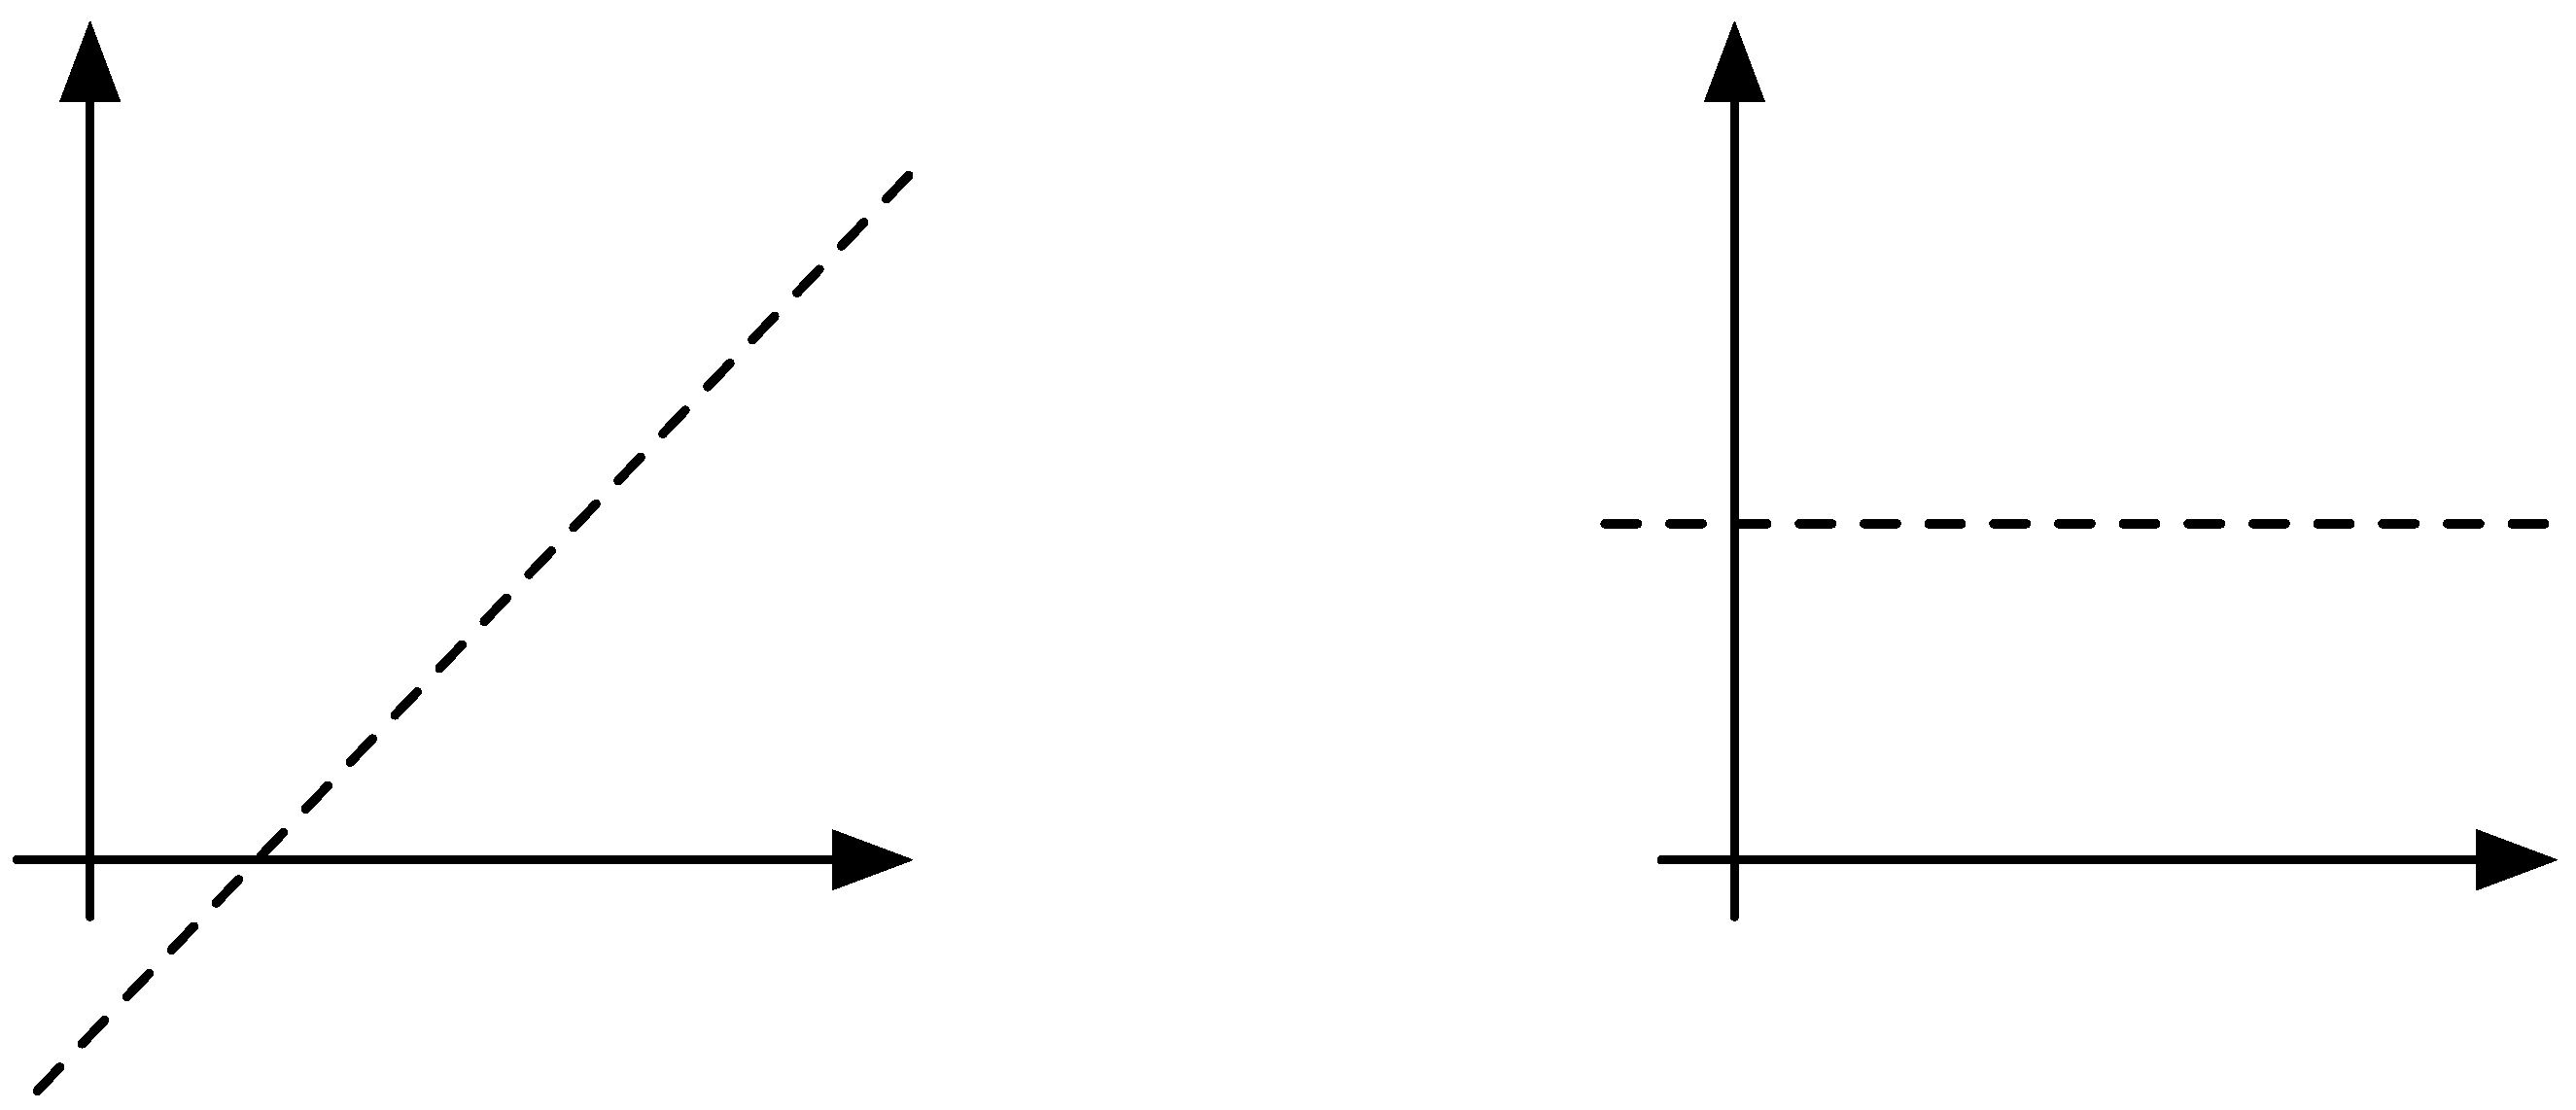
\includegraphics[width=3in]{Pictures/lineSoln.pdf}
\end{center}
One way of dealing with this is for the
function to return a \texttt{(Float,Bool)} pair. If the boolean part is {\mi
False}, this signals that no solution was found; if it is like {\mi
(2.1,True)}, it indicates that \texttt{2.1} is indeed the solution.
\end{example}

\subsection*{Pattern matching}

Next we turn to look at how functions can be defined over tuples.
Functions over tuples are usually defined by \textbf{pattern matching}\index{pattern matching}.
Instead of writing
a variable for an argument of type \texttt{(Integer,Integer)}, say, a \textbf{pattern},
\index{pattern}
\texttt{(x,y)}
is used. 
\begin{alltt}
addPair :: (Integer,Integer) -> Integer\minx{addPair}
addPair (x,y) = x+y
\end{alltt}
On application the components of the pattern
are matched by the corresponding components of the argument, so that on
applying the function \texttt{addPair} to the argument \texttt{(5,8)}
the value \texttt{5} is matched to \texttt{x}, and \texttt{8} to
\texttt{y}, giving the calculation
\begin{alltt}
addPair (5,8) 
\step 5+8
\step 13
\end{alltt}
Patterns can contain literals and nested patterns,\index{pattern!nested}
as in the examples
\begin{alltt}
addPair (0,y) = y
addPair (x,y) = x+y

shift :: ((Integer,Integer),Integer) -> (Integer,(Integer,Integer))
shift ((x,y),z) = (x,(y,z))
\end{alltt}
Functions which pick out particular parts of a tuple can be defined by
pattern matching. For the \texttt{ShopItem} type, the definitions might be
\begin{alltt}
name  :: ShopItem -> String
price :: ShopItem -> Int

name  (n,p) = n
price (n,p) = p
\end{alltt}
Haskell has these \textbf{selector functions} on pairs built in. They are
\index{selector}\index{function!selector}
\begin{alltt}
fst (x,y) = x\minx{fst}
snd (x,y) = y\minx{snd}
\end{alltt}
Given these selector functions we can avoid pattern matching if
we so wish. For instance, we could redefine \texttt{addPair} like this
\begin{alltt}
addPair :: (Integer,Integer) -> Integer\minx{addPair}
addPair p = fst p + snd p
\end{alltt}
but generally a pattern-matching definition is easier to read than
one which uses selector functions instead.


\begin{example}
\subexample*{3.} 
We first introduced the Fibonacci numbers\index{Fibonacci numbers} 
\begin{alltt}
0, 1, 1, 2, 3, 5, ... , u, v, (u+v), ...
\end{alltt}
in Section \ref{genRecursion}, where we gave an inefficient recursive definition of
the sequence. Using a tuple we can give an efficient
solution to the problem. The next value in the sequence is given by
adding the previous two, so what we do is to write a function which
returns {\em two consecutive values\/} as a result. In other words we want to define
a function \texttt{fibPair} so that it has the property that
\begin{alltt}
fibPair n = (fib n , fib (n+1))
\end{alltt} 
then given such a pair, \texttt{(u,v)} we get the next pair as
\texttt{(v,u+v)}, which is exactly the effect of the \texttt{fibStep} function:
\begin{alltt}
fibStep :: (Integer,Integer) -> (Integer,Integer)\minx{fibStep}
fibStep (u,v) = (v,u+v)
\end{alltt}
This gives us the definition of the `Fibonacci pair' function
\begin{alltt}
fibPair :: Integer -> (Integer,Integer)\minx{fibPair}
fibPair n
  | n==0        = (0,1)
  | otherwise   = fibStep (fibPair (n-1))
\end{alltt}
and we can define
\begin{alltt}
fastFib :: Integer -> Integer\minx{fastFib}
fastFib = fst . fibPair
\end{alltt}
where recall that `\texttt{.}'\minx{.} composes the two functions, passing the
output of \texttt{fibPair}
to the input of \texttt{fst}, which picks out its first component.
\end{example}

\beware{One pair or two arguments?}{\index{pitfalls!paired arguments}\index{argument!tuple}
It is important to distinguish between the functions\minx{fibStep}\minx{fibTwoStep}
\begin{alltt}
fibStep :: (Integer,Integer) -> (Integer,Integer)\\
fibStep (x,y) = (y,x+y)\\
\ \\
fibTwoStep :: Integer -> Integer -> (Integer,Integer)\\
fibTwoStep x y = (y,x+y)
\end{alltt}
\texttt{fibStep} has a single argument which is a pair of numbers,
while \texttt{fibTwoStep} has two arguments, each of which is
a number. We shall see later that the second function
can be used in a more flexible way than the first; for the moment it is
important to realize that there is a difference, and that type errors will
result if we confuse the two and write\index{type error}
\begin{alltt}
fibStep 2 3\ \ \ \ \ \ \ \ \ \ \ \ \ \ \ \ \ \ \ \ \ fibTwoStep (2,3)
\end{alltt}
We say more about the relationship between these two functions in Section
\ref{curry}.
}

\begin{exercises}
\item
Give a definition of the function
\begin{alltt}
maxOccurs :: Integer -> Integer -> (Integer,Integer)
\end{alltt}
which returns the maximum of two integers, together with the number of times
it occurs. Using this, or otherwise, define the function
\begin{alltt}
maxThreeOccurs :: Integer -> Integer -> Integer -> (Integer,Integer)
\end{alltt}
which does a similar thing for three arguments.

\item
Give a definition of a function
\begin{alltt}
orderTriple :: (Integer,Integer,Integer) -> (Integer,Integer,Integer)
\end{alltt} 
which puts the elements of a triple of three integers into ascending order.
You might like to use the \texttt{maxThree}, \texttt{middle} and
\texttt{minThree} functions defined earlier.

\item
Define the function which finds where a straight line crosses the x-axis. 
You will need to think about how to supply the information about the
straight line to the function.

\item Design test data for the preceding exercises; explain the choices you
have made in each case. Give a sample evaluation of each of your functions.
\index{tuples|)}

\end{exercises}



\section{Introducing algebraic types}
\label{introAlg}\index{type!algebraic|see{algebraic type}}\index{algebraic type|(}

We have already seen that it's useful to be able to define our own enumerated types, such as a move in the Rock - Paper - Scissors game, a day of the week, or a season of the year. In this section we'll see that we can use \texttt{data} types for much more general combinations of values. 


Algebraic data type definitions are introduced by the keyword \texttt{data}, followed by 
the name of the type, an equals sign and then information about how elements are constructed by applying 
\textbf{constructors}.\index{constructor}  The names of the type and the constructors begin with
capital letters.

We give a sequence of examples of increasing complexity, first recapping enumerated types, then looking at single constructor product types, and finally looking at types which contain a number of alternative `shapes' of data. We look again at \texttt{data} types in Chapter \ref{algTypes}.

\subsection*{Enumerated types}
\index{enumerated type}

We have already seen examples of this, such as the type modelling a move in the Rock - Paper - Scissors game, in Section \ref{EnumTypes}. Recall that the definition lists the elements of the type, thus: 
\begin{alltt}
data Move = Rock | Paper | Scissors \minx{Move}
            deriving (Eq,Show)
\end{alltt}
and we can define functions by pattern matching over the values, as in
\begin{alltt}\minx{score}
score :: Move -> Move -> Integer
score Rock Rock     = 0
score Rock Paper    = -1
score Rock Scissors = 1
score Paper Rock    = 1
\end{alltt}
As we noted in Section \ref{EnumTypes} we can derive definitions of functions like equality using a `\texttt{deriving}' clause in the definition of a \texttt{data} type so that we don't need to define these functions for ourselves when we introduce a new data type definition. We will talk about the details of what underlies this in Section \ref{algClasses}.
 
 
\subsection*{Product types}
\index{product type}

Instead of using a tuple we can define a \texttt{data} type with a number of
components or fields, often called a \textbf{product} type. An
example might be
\begin{alltt}\minx{Person}\minx{People}
data People = Person Name Age \hfill (People)
              deriving (Eq,Show)
\end{alltt}
where \texttt{Name} is a synonym for \texttt{String}, and \texttt{Age} for \texttt{Int},
written thus:
\begin{alltt}
type Name = String
type Age  = Int
\end{alltt}
The definition of \texttt{People} should be read as saying
\[
\parbox{28pc}{To construct an element of type \texttt{People}, you need to supply two values;
one,
\texttt{st} say, of
type \texttt{Name}, and another, \texttt{n} say, of type \texttt{Age}. The
element of \texttt{People} formed from them will be \texttt{Person st n}.} 
\]
Example values of this type include\index{Jemima, Electric Aunt}
\begin{alltt}
Person "Electric Aunt Jemima" 77
Person "Ronnie" 14
\end{alltt}
As before,  
functions are defined using \textbf{pattern matching}. Any element of type 
\texttt{People} will have the form \texttt{Person st n}, and so we can use this pattern on the
left-hand side of a definition,
\begin{alltt}
showPerson :: People -> String
showPerson (Person st n) = st ++ " -- " ++ show n
\end{alltt}
(recall that \texttt{show} gives a textual form of an \texttt{Int}). For instance,\index{Jemima, Electric Aunt}
\index{Electric Aunt Jemima|see{Jemima, Electric Aunt}}
\begin{alltt}
showPerson (Person "Electric Aunt Jemima" 77)
 = "Electric Aunt Jemima -- 77"
\end{alltt}
Elements of the \texttt{People} type are made (or \texttt{constructed}) by applying the \textbf{constructor} \texttt{Person}. This is called a 
\textbf{binary} constructor
\index{constructor!binary}
because it takes two values to form a value of type 
\texttt{People}. For the enumerated types like \texttt{Move} the constructors
are called \textbf{nullary}
\index{constructor!nullary}
(or {\em 0-ary}) as they take no arguments. 
 
The constructors introduced by algebraic type definitions can be used
just like functions, so that \texttt{Person st n} is the result of applying
the function \texttt{Person} to the arguments \texttt{st} and \texttt{n}; we can
interpret the definition \texttt{(People)} as giving the \textbf{type of the constructor}, here
\begin{alltt}
Person :: Name -> Age -> People
\end{alltt}

\begin{figure}[t]
\beware{Tuples and \texttt{data} types}{\index{type!tuples and \texttt{data} types}
An alternative definition of the type of people is given by the type
synonym
\begin{alltt}
type People = (Name,Age)
\end{alltt}
The advantages of using an algebraic type are threefold.
\begin{titemize}\index{algebraic type!compared with tuple}
\index{tuples!compared with algebraic type}
\item Each object of the type carries an explicit \textbf{label} of the
purpose of the element; in this case that it represents a person.
\item It is not possible accidentally to treat an arbitrary pair consisting of
a string and a number as a person; a person must be constructed using the
\texttt{Person} constructor.
\item The type will appear
in any error messages due to mis-typing; a type synonym might be expanded out 
and so disappear from any type error messages.
\end{titemize} 
There are also advantages of using a tuple type, with a synonym declaration.
\begin{titemize}
\item The elements are more compact, and so definitions will be shorter.
\item Using a tuple, especially a pair, allows us to reuse many 
polymorphic functions such as \texttt{fst}, \texttt{snd} and
\texttt{unzip} over tuple types; this will not be the case for the
algebraic type.
\end{titemize}
In each system that
we model we will have to choose between these alternatives: our
decisions will depend exactly on how we use the products, and on the
complexity of the system.


The approach here works equally well with unary constructors, so we
\index{constructor!unary}
might say
\begin{alltt}
data Age = Years Int
\end{alltt}
whose elements are \texttt{Years 45} and so on. It is clear from a definition
like this that \texttt{45} is here being used as an age in years, rather than
some unrelated numerical quantity. The disadvantage is that we cannot use
functions defined over \texttt{Int} directly over \texttt{Age}.
}\end{figure}

\begin{figure}[t]
\beware{Type and constructor names}{\index{pitfalls!type and constructor names}
We can use the same name, for instance \texttt{Person}, for both the type and the
constructor of a type, as in the definition
\begin{alltt}
data Person = Person Name Age
\end{alltt}
We choose not to do this, as using the same name for two related but
different objects can easily lead to confusion, but it is an idiom used
by a number of Haskell programmers and in many Haskell libraries.
}\end{figure}
The examples of types given here are a special case of what we look at next.


\subsection*{Alternatives}
\index{algebraic type!alternatives}

A shape in a simple geometrical program is either a circle or a
rectangle. These alternatives are given by the type
\begin{alltt}\minx{Circle}\minx{Rectangle}
data Shape = Circle Float |\hfill(Shape)\minx{Shape}
             Rectangle Float Float
             deriving (Eq,Ord,Show)
\end{alltt}
which says that there are two ways of building an element of \texttt{Shape}. One
way is to supply the radius of a \texttt{Circle}; the other alternative is to give
the sides of a \texttt{Rectangle}. Example objects of this type are

\begin{alltt}
Circle 3.0
Rectangle 45.9 87.6
\end{alltt}
Pattern matching allows us to define functions by cases, as
in\index{algebraic type!pattern matching}
\index{pattern matching!algebraic type}
\begin{alltt}
isRound :: Shape -> Bool
isRound (Circle _)      = True
isRound (Rectangle _ _) = False
\end{alltt}
and also lets us use the 
components of the elements:
\begin{alltt}\label{areaDef}
area :: Shape -> Float
area (Circle r)      = pi*r*r
area (Rectangle h w) = h*w
\end{alltt}
Another way of reading the definition \texttt{(Shape)} is to say that
there are two \textbf{constructor functions} for the type \texttt{Shape}, whose
types are
\begin{alltt}
Circle    :: Float -> Shape
Rectangle :: Float -> Float -> Shape
\end{alltt}
These functions are called constructor functions because the elements of
the type are constructed by applying these functions.

Extensions of this type, to accommodate the position of an object, are
discussed in the exercises at the end of this section.

\subsection*{The general form of algebraic type definitions}
\index{algebraic type!general form}

The general form of the algebraic type definitions which we have seen so far is
\begin{alltt}
data Typename \hfill (Typename)
  = \subscr{Con}{1} \subscr{t}{11} \ldots \subscr{t}{1\subscr{k}{1}} | 
    \subscr{Con}{2} \subscr{t}{21} \ldots \subscr{t}{2\subscr{k}{2}} | 
        ....
    \subscr{Con}{n} \subscr{t}{n1} \ldots \subscr{t}{n\subscr{k}{n}}   
\end{alltt}
Each \texttt{\subscr{Con}{i}} is a constructor, followed by 
\subscr{k}{i}\ types, where \subscr{k}{i}\ is a non-negative integer which may
be zero. We build elements of the type \texttt{Typename} by applying these constructor
functions to arguments of the types given in the definition, so that
\begin{alltt}
\subscr{Con}{i} \subscr{v}{i1} \ldots \subscr{v}{i\subscr{k}{i}}
\end{alltt}
will be a member of the type \texttt{Typename} if \subscr{v}{ij} is 
in \subscr{t}{ij} for \texttt{j} ranging from \texttt{1} to \subscr{k}{i}. 

Reading the constructors as functions, the 
definition \texttt{(Typename)} gives the constructors the following
types
\begin{alltt}
\subscr{Con}{i} :: \subscr{t}{i1} -> \ldots -> \subscr{t}{i\subscr{k}{i}} -> Typename
\end{alltt}
In Chapter \ref{algTypes} we shall see two
extensions of the definitions seen already. 
\begin{titemize}
\item The types can be \textbf{recursive}\index{algebraic type!recursive|see{recursive type}};
we can use the type we are defining,
\texttt{Typename}, as (part of) any of the types \subscr{t}{ij}. This gives us
lists, trees and many other data structures.
\item The \texttt{Typename} can be followed by one or more type
variables which may be used on the right-hand side, making the definition
\textbf{polymorphic}. 
\end{titemize}
Recursive polymorphic types combine these two ideas, and this powerful
mixture provides types which can be reused in many different situations --
the built-in type of lists is an example of this kind of type. We look at these in Chapter \ref{algTypes}.

For the moment, however, we'll deal with the simple cases we have covered in this section, which are enough to model a wide variety of different problem domains, particularly in conjunction with tuples and lists.

\begin{figure}[t]
\beware{\texttt{type} and \texttt{data} definitions}{\index{pitfalls!\texttt{type} and \texttt{data}}
\index{type@\texttt{type} and \texttt{data}}Before we move on, it is worth contrasting \texttt{type} and \texttt{data} definitions.
A synonym given by \texttt{type} is simply a shorthand, and so a synonym type can always be
expanded out, and therefore removed from the program. 

\medskip
\noindent
On the other hand, a \texttt{data}
definition creates a new type. Because synonyms are simply shorthand, a
synonym definition cannot be recursive; \texttt{data} definitions can be
and often are recursive, as we shall discover in Chapter \ref{algTypes}.
}\end{figure}





\begin{exercises}


\item
Define a function to give the length of the perimeter of a geometrical shape,
of type \texttt{Shape}. What is the type of this function?

\item
Re-define the \texttt{Item} type for supermarket products so that it uses a \texttt{data} definition rather than a \texttt{type} definition.

\item
Add an extra constructor to \texttt{Shape} for triangles, and extend the
functions \texttt{isRound}, \texttt{area} and \texttt{perimeter} to include triangles.

\item
Define a function which decides whether a \texttt{Shape} is regular: a circle is
regular, a square is a regular rectangle and being equilateral makes a
triangle regular.

\item
Investigate the derived definitions for \texttt{Move} and \texttt{Shape}: what form
do the  \texttt{show} functions take, for example?

\item
Define an \texttt{==} function over \texttt{Shape} so that all circles of negative radius are
equated. How would you treat rectangles with negative sides?

\item
The type \texttt{Shape} takes no account of the position or orientation of a 
shape. After deciding how to represent points, how would you modify the
original definition of \texttt{Shape} to contain the \textbf{centre} of each object? You
can assume that rectangles lie with their sides parallel to the axes, thus:
\begin{center}
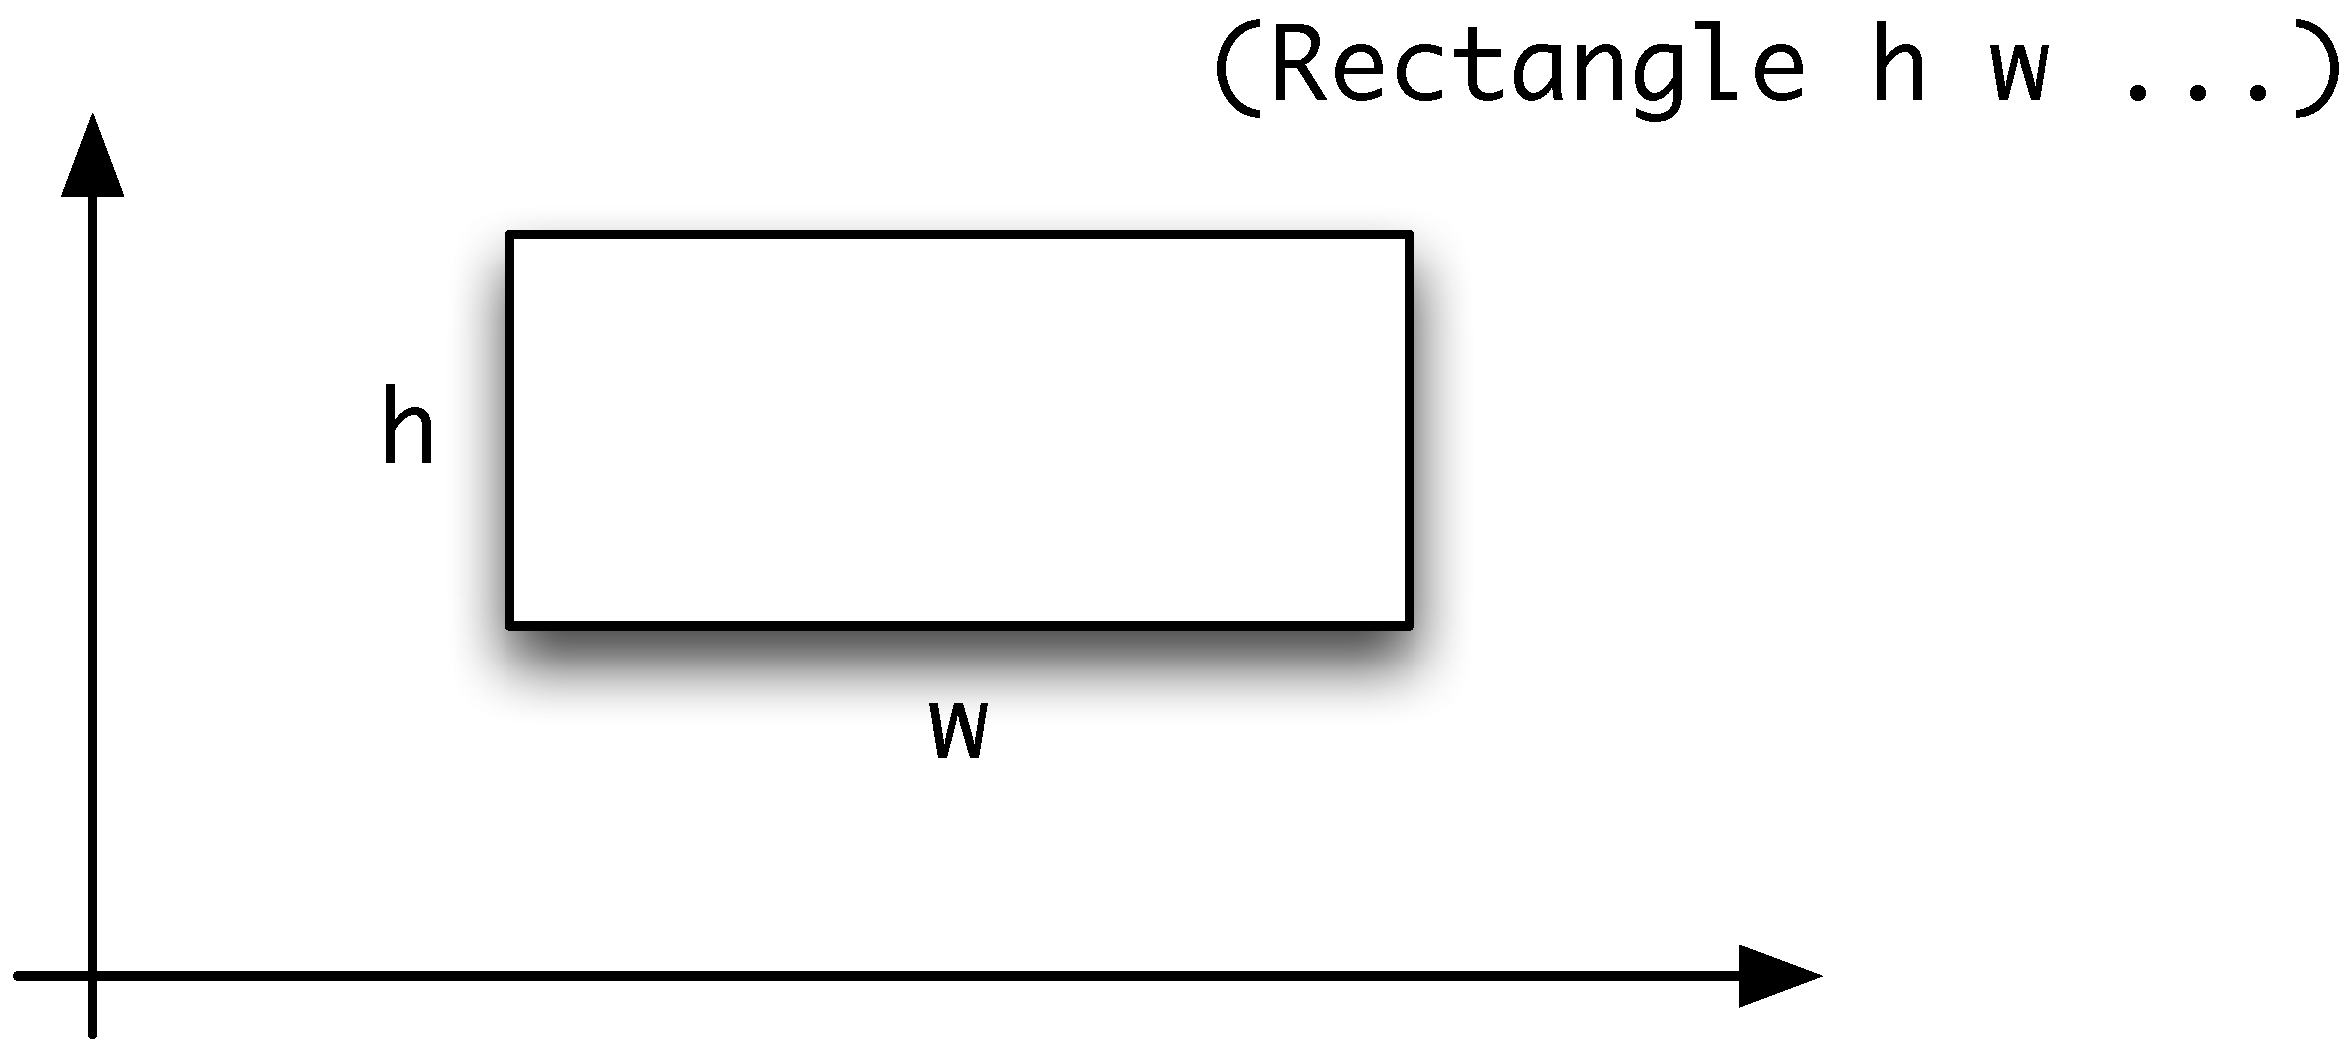
\includegraphics[width=3in]{Pictures/rectanglePos.pdf}
\end{center}

\item
Calling the new shape type \texttt{NewShape}, define a function 
\begin{alltt}
move :: Float -> Float -> NewShape -> NewShape 
\end{alltt}
which moves a shape by the two offsets given:
\begin{center}
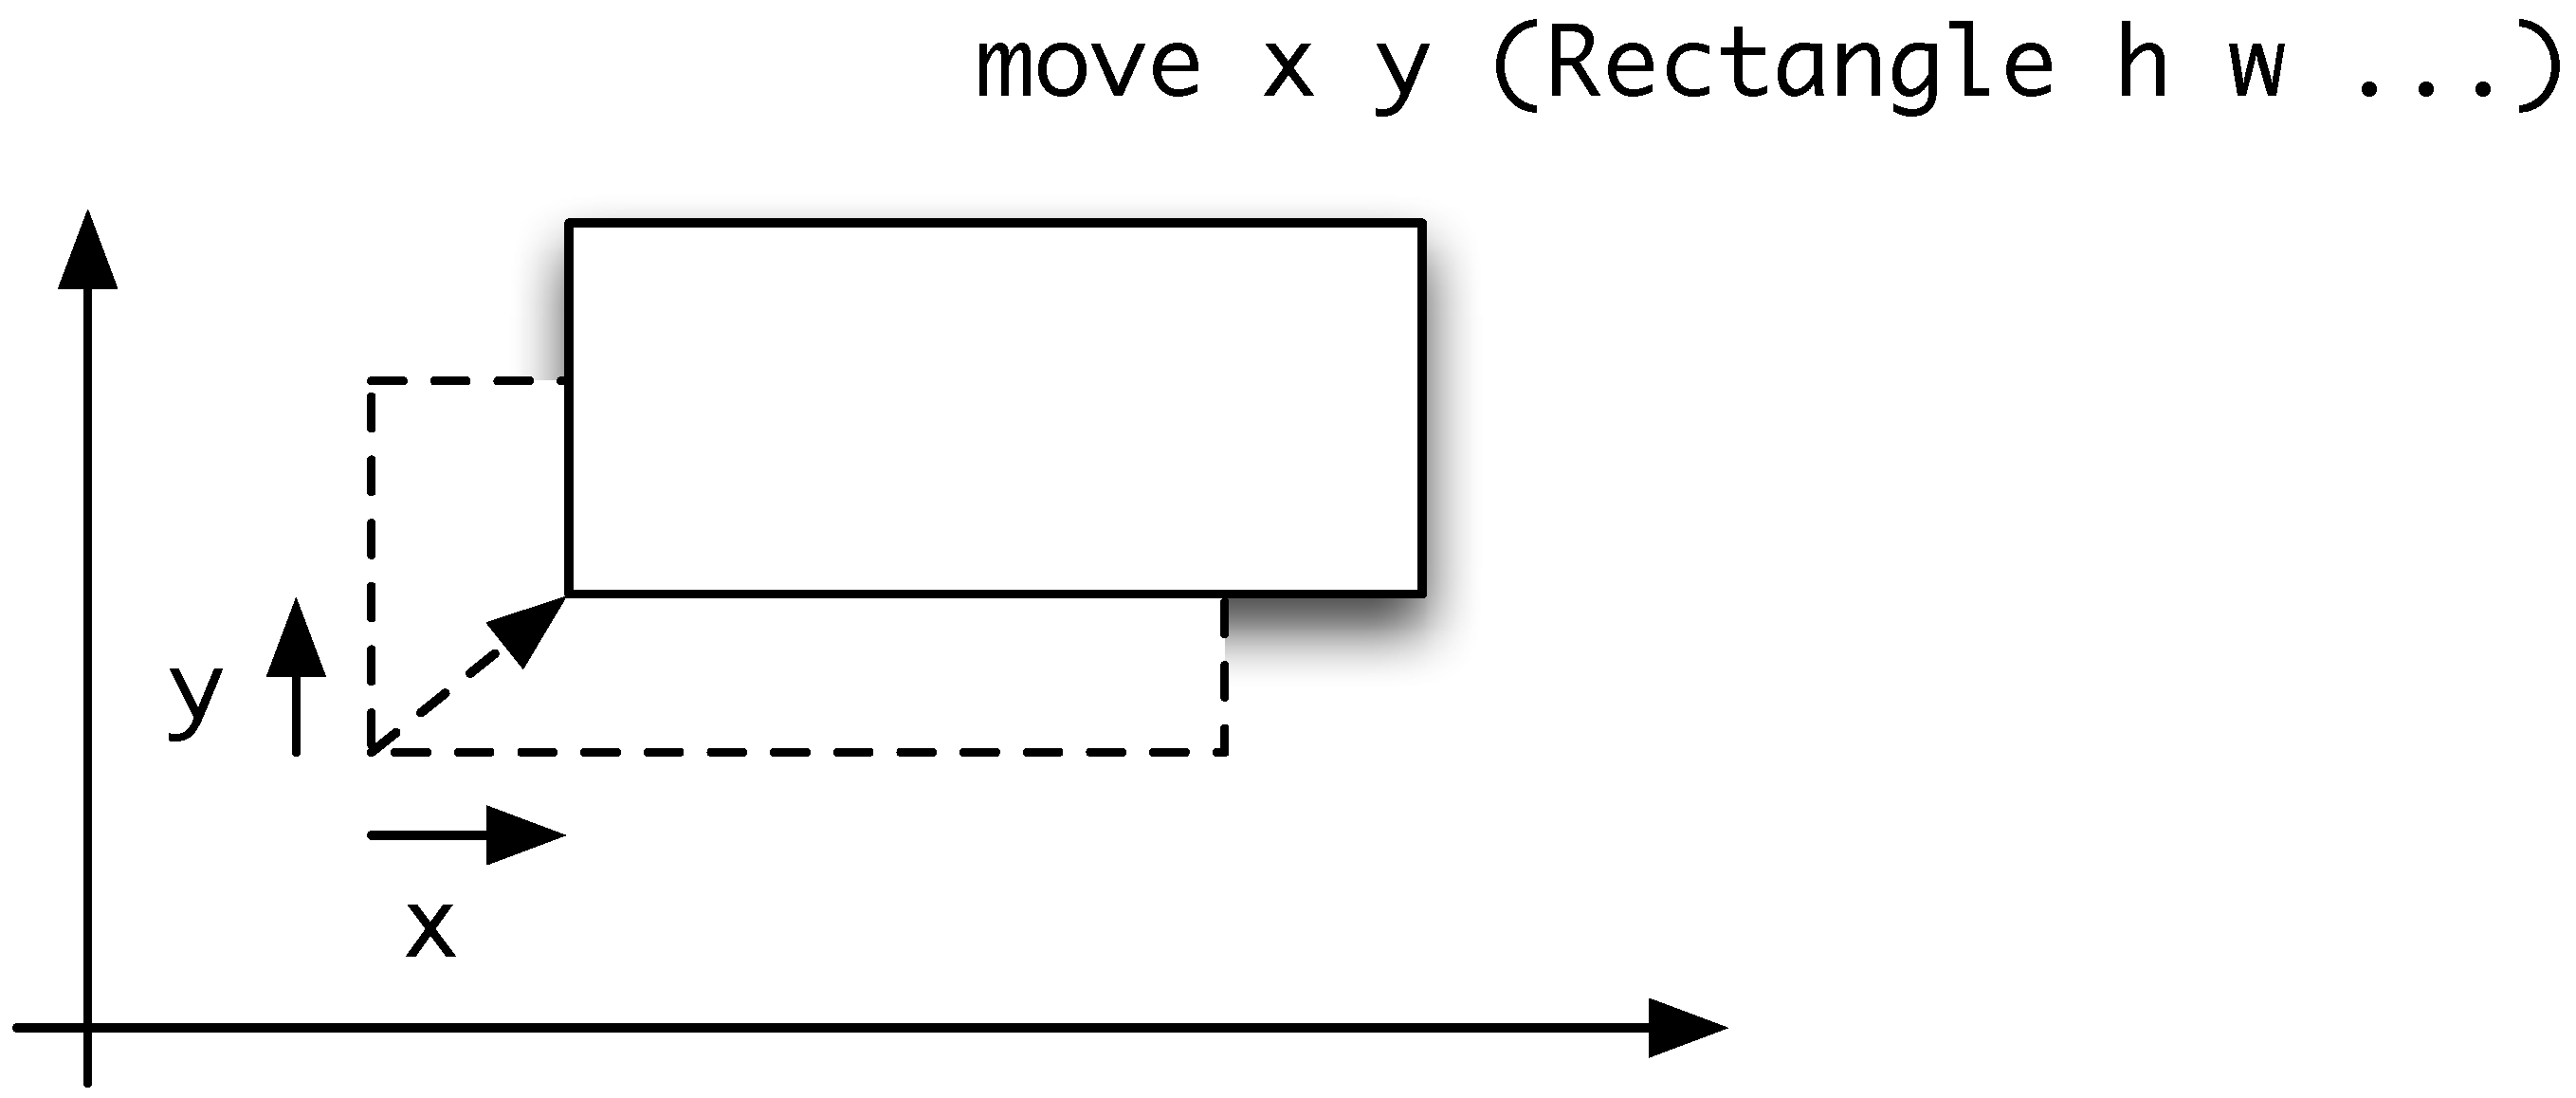
\includegraphics[width=3.5in]{Pictures/rectangleMove.pdf}
\end{center}


\item
Define a function to test whether two \texttt{NewShapes} overlap.

\item
Some houses have a number; others have a name.
How would you implement the type of `strings or numbers' used as a part of an
address? Write a function which gives the textual form of one of these objects. Give a
definition of a type of names and addresses using the type you have defined.


\end{exercises}


\index{algebraic type|)}


\section{Our approach to lists}
\index{lists|(}
\index{lists!approach taken}


Lists are a remarkably expressive data type. We can represent a text as
a list of lines, each of which is a list of words; we can represent a
collection of information, like a supermarket bill, as a list of
individual items of data; we can represent a collection of readings from
a measuring device as a list of \texttt{Floats}, to mention but three
potential applications. 

At the same time, there are many different things which we can
do to lists, some of which first came out in our implementation of \texttt{Pictures}
by lists\minx{Picture}
in Chapter \ref{intro}. Given a list we can split it up according to
various criteria, we can sort it, select items from it and transform all
its members in a particular way. We can combine lists by joining them
together or by coalescing corresponding elements. We can combine all
the members of a list together -- by taking their sum, maximum or
conjunction, say -- among many other operations. 
Haskell contains many built-in list functions
and operators in the standard prelude \texttt{Prelude.hs}\minx{Prelude.hs}
and also various library modules, including
\texttt{List.hs}. \minx{List.hs}

Because Haskell has so many list functions built in, we can approach our discussion of
lists in two very different ways. We could argue that we should start by 
defining list-manipulating functions for ourselves, and only use library
functions after we have understood their definitions.\footnote{This was
essentially the approach taken in the first edition of this book.} On
the other hand, we could adopt a `toolkit' approach, and simply discuss
the library functions and how they can be used. What we aim to do here
is to combine the two approaches, often introducing and using functions
before they are defined explicitly, but then looking `under the bonnet' to see
how these functions are defined  and how we can define other functions
for ourselves. 


In the remainder of this chapter we introduce some of the facilities for
list manipulation within Haskell, particularly \emph{list comprehensions} which give a flexible notation for transforming and selecting elements of lists. This is followed in Chapter \ref{progLists} with an overview of the list functions available to the Haskell programmer, and in Chapter \ref{defFunLists} we see how to define these and
other functions for ourselves.




\section{Lists in Haskell}

A list in Haskell is a collection of items from a given type. For every type \texttt{t}
there is a Haskell type \texttt{[t]} of lists of elements from \texttt{t}.
\begin{alltt}
[1,2,3,4,1,4] :: [Integer]
[True]        :: [Bool]
\end{alltt}
We read these as `\texttt{[1,2,3,4,1,4]} is a list of \texttt{Integer}' and
`\texttt{[True]} is a list of \texttt{Bool}'. \texttt{String} is a synonym
\minx{String}
for {\mi
[Char]} and the two lists which follow are the same.
\begin{alltt}
['a','a','b'] :: String
"aab"         :: String
\end{alltt}
We can build lists of items of any particular type, and so we can have lists of
functions and lists of lists of numbers, as in
\begin{alltt}
[fastFib,fastFib]  :: [ Integer -> Integer ]
[[12,2],[2,12],[]] :: [ [Integer] ]
\end{alltt}
As can be seen, the list with elements \texttt{\eone}, \texttt{\etwo}, \texttt{\subscr{e}{3}}, \texttt{\subscr{e}{4}} and \texttt{\subscr{e}{5}}  is written by enclosing the elements in square brackets, separated by commas, like this
\begin{alltt}
[\texttt{\eone},\texttt{\etwo},\texttt{\subscr{e}{3}},\texttt{\subscr{e}{4}},\texttt{\subscr{e}{5}}]
\end{alltt}
As a special case the empty list, \texttt{[]},\minx{[]} which contains no items, is
an element of every list type.

The order of the
items in a list is significant, as is the number of times that an item
appears. The three lists of numbers which follow are therefore all
different:
\begin{alltt}
[1,2,1,2,2]
[2,1,1,2,2]
[2,1,1,2]
\end{alltt}
The first two have length \texttt{5}, while the third has length
\texttt{4}; the first element of the first list is \texttt{1}, while
the first element of the second is \texttt{2}. A set\index{sets} is another kind of
collection in which the ordering of items and the number of 
occurrences of a particular item are not relevant; we look at sets in Chapter \ref{adt}.

There are some other ways of writing down lists of numbers, characters and other enumerated
types 
\begin{itemize}
\item \texttt{[n ..\ m]} is the list \texttt{[n,n+1,\ldots,m]}; if \minx{..}
\texttt{n} exceeds \texttt{m}, the list is empty.
\begin{alltt}
[2 ..\ 7]     \step{}[2,3,4,5,6,7]
[3.1 ..\ 7.0] \step{}[3.1,4.1,5.1,6.1,7.1]
['a' ..\ 'm'] \step{}"abcdefghijklm"
\end{alltt}
\item \texttt{[n,p ..\ m]} is the list of numbers whose first two elements are \texttt{n} and
\texttt{p} and whose last is \texttt{m}, with the numbers ascending in steps
of \texttt{p-n}. For example,
\begin{alltt}
[7,6 ..\ 3]       \step{}[7,6,5,4,3]
[0.0,0.3 ..\ 1.0] \step{}[0.0,0.3,0.6,0.8999999999999999]
['a','c' ..\ 'n'] \step{}"acegikm"
\end{alltt}
\item In both cases it can be seen that if the step size does not allow us to
reach \texttt{m} exactly, the last item of the list is the element in the
sequence that is closest to \texttt{m}, even if it appears to ``overshoot'' the limit. It can also
be the case that rounding errors on \texttt{Float} lead to lists being
different from what is anticipated; an example is given in the
exercises.
\end{itemize}
In the next section we turn to a powerful method of writing down lists which we can use to define
a variety of list-manipulating functions. 

\subsection*{The \texttt{String} type}
\index{strings|(}
\minx{String}

We first introduced the string type \texttt{String} in Section \ref{char}, and saw there that strings are sequences of characters, that is sequences of \texttt{Char}s. In fact, the \texttt{String} type is a special case of lists, 
\begin{alltt}
type String = [Char]
\end{alltt}
and all the polymorphic prelude functions in Figure \ref{polyListOps}
can be used over strings. We saw in Section \ref{char} how to write
the special characters such as newline and tab using the `escapes'
\texttt{'\bs{n}'} and \texttt{'\bs{t}'}, and also how we could join strings using `\texttt{++}': of course, we can use that operator on \emph{any} list type. 
Other functions over strings can be found in the library \texttt{Data.String}.\minx{Data.String}

%\subsection*{Strings and values}

Built into Haskell are the overloaded functions \texttt{show}\index{show@\texttt{show}}
and \texttt{read}\minx{read}, which convert from a value to a
\texttt{String} and
vice versa; for instance,
\begin{alltt}
show (2+3)           \step{}"5"
show (True || False) \step{}"True"
\end{alltt}
In the opposite direction, the function \texttt{read} is used to convert
a string to the value it represents, so that
\begin{alltt}
read "True" \step{}True
read "3"    \step{}3
\end{alltt}
In some situations it will not be clear what should be the result type
for
\texttt{read} -- it is then possible to give a type to the application,
as in
\begin{alltt}
(read "3") :: Integer
\end{alltt}
the  result of which will be \texttt{3} and its type, \texttt{Integer}. 

We saw in Section \ref{char} that \texttt{show} and \texttt{read} could be used to and from \texttt{String} from other types; a
full explanation of the types of \texttt{read} and \texttt{show} can be
found in Chapter \ref{typeClasses}.
\index{strings|)}


\begin{exercises}

\item
What value has the expression \texttt{[0, 0.1 ..\ 1]}? Check your answer
in GHCi  and explain any discrepancy there might be between the two.

\item
How many items does the list \texttt{[2,3]} contain? How many does \texttt{[[2,3]]}
contain? What is the type of \texttt{[[2,3]]}?

\item
What is the result of evaluating \texttt{[2 ..\ 2]}? What about \texttt{[2,7 ..\ 4]}?
Try evaluating \texttt{[2,2 ..\ 2]}; to \textbf{interrupt evaluation}\index{evaluation!interrupt}
\minx{Ctrl-C} in GHCi under Windows or Unix you
need to type \texttt{Ctrl-C}.
\end{exercises}



\section{List comprehensions}
\label{listComps}
\index{list comprehensions|(}

One of the distinct features of a functional language is the list
comprehension notation, which has no parallels in other paradigms.

In a list comprehension we write down a description of a list in terms
of the elements of another list. From the first list we
\textbf{generate} elements, which we \textbf{test} and
\textbf{transform} to form elements of the result. We will describe 
list comprehensions with a single generator in this section; Section
17.3 covers the general case. Nevertheless, the simple case we
look at here is very useful in writing a variety of list-processing
programs. We introduce the topic by a series of examples.

\begin{example}
\subexample*{1.}
Suppose that the list \texttt{ex} is \texttt{[2,4,7]}, then the list
comprehension
\begin{alltt}
[ 2*n | n<-ex]\hfill (1)
\end{alltt}
will be
\begin{alltt}
[4,8,14]
\end{alltt}
as it contains each of the elements \texttt{n} of the list \texttt{ex}, doubled:
\texttt{2*n}. We can read \texttt{(1)} as saying
\begin{quote}
`Take all \texttt{2*n} where \texttt{n} comes from \texttt{ex}.'
\end{quote}
where the symbol \texttt{<-}\minx{<-} is meant to resemble the mathematical symbol for
being an element, `$\in$'. We can write the evaluation of the list
comprehension in a table, thus:
\begin{alltt}
[ 2*n | n <- [2,4,7] ] 
 
  n   =   2   4   7
2*n   =   4   8  14
\end{alltt}

\subexample*{2.}
In a similar way, 
\begin{alltt}
[ isEven n | n<-ex ] \step{}[True,True,False]
\end{alltt}
if the function \texttt{isEven} has the 
definition
\begin{alltt}
isEven :: Integer -> Bool
isEven n = (n `mod` 2 == 0)
\end{alltt} 
In
list comprehensions \texttt{n<-ex} is called a {\bf generator} because it
\index{list comprehensions!generator}
generates the data from which the results are built. On the left-hand side
of the `\texttt{<-}'\minx{<-}
there is a variable, \texttt{n}, while on the right-hand
side we put the list, in this case \texttt{ex}, from which the elements are taken.


\subexample*{3.}
We can combine a generator with one or more {\bf tests}, 
\index{list comprehensions!test} which are Boolean
expressions, thus:
\begin{alltt}
[ 2*n | n <- ex , isEven n , n>3 ]\hfill (2)
\end{alltt}
\texttt{(2)} is paraphrased as
\begin{quote}
`Take all \texttt{2*n} where \texttt{n} comes from \texttt{ex}, \texttt{n} is even and
greater than \texttt{3}.'
\end{quote}
Again, we can write the evaluation in tabular form.
\begin{alltt}
[ 2*n | n <- [2,4,7] , isEven n , n>3 ]
 
       n   =   2   4   7
isEven n   =   T   T   F
     n>3   =   F   T   
     2*n   =       8   
\end{alltt}
The result of \texttt{(2)} will therefore be the list \texttt{[8]}, as \texttt{4} is
the only even element of \texttt{[2,4,7]} which is greater than \texttt{3}.

\subexample*{4.}
Instead of placing a variable to the left of the arrow `\texttt{<-}', we can put
a pattern. For instance,
\begin{alltt}
addPairs :: [(Integer,Integer)] -> [Integer]\minx{addPairs}
addPairs pairList = [ m+n | (m,n) <- pairList ]
\end{alltt}
Here we choose all the pairs in the list \texttt{pairList}, and add their
components to give a single number in the result list. For example,
\begin{alltt}
[ m+n | (m,n) <- [(2,3),(2,1),(7,8)] ]
 
  m   =   2   2   7  
  n   =   3   1   8
m+n   =   5   3  15
\end{alltt}
giving the result 
\begin{alltt}
addPairs [(2,3),(2,1),(7,8)] \step{}[5,3,15]
\end{alltt}

\subexample*{5.}
We can add tests in such a situation, too:
\begin{alltt}
addOrdPairs :: [(Integer,Integer)] -> [Integer]
addOrdPairs pairList = [ m+n | (m,n) <- pairList , m<n ]
\end{alltt}
so that with the same input example, 
\begin{alltt}
[ m+n | (m,n) <- [(2,3),(2,1),(7,8)] , m<n ]
 
  m   =   2   2   7  
  n   =   3   1   8
m<n   =   T   F   T
m+n   =   5      15
\end{alltt}
giving 
\begin{alltt}
addOrdPairs [(2,3),(2,1),(7,8)] \step{}[5,15]
\end{alltt}
since the second pair in the list, \texttt{(2,1)}, fails the test.

\subexample*{6.}
Note that we can simply test elements, with the
effect that we filter some of the elements of a list, according to a
Boolean condition. To find all the digits in a string we can say
\begin{alltt}
digits :: String -> String\minx{digits}
digits st = [ ch | ch<-st , isDigit ch ] 
\end{alltt}
where the function
\begin{alltt}
isDigit :: Char -> Bool
\end{alltt}
imported from the module \texttt{Data.Char} is \texttt{True} on those characters which are digits: \texttt{'0'},
\texttt{'1'} up to \texttt{'9'}.

\subexample*{7.}
A list comprehension can form a part of a larger function definition.
Suppose that we want to check whether all members of a list of integers
are even, or all are odd. We can write
\begin{alltt}
allEven xs = (xs == [x | x<-xs, isEven x])
allOdd xs  = ([] == [x | x<-xs, isEven x])
\end{alltt}
We will see list comprehensions in practice in the next section when we
examine a simple library database.


\subexample*{8.}
The pattern on the left-hand side of an arrow need not match everything in the list: take the example
\begin{alltt}
totalRadii :: [Shape] -> Float
totalRadii shapes = sum [r | Circle r <- shapes]
\end{alltt}
The effect of this is to match only the circles in the \texttt{shapes} list, and to ignore any other shapes, so that, for example
\begin{alltt}
totalRadii [Circle 2.1, Rectangle 2.1 3.2, Circle 4.7] \step{}6.8
\end{alltt}
This also applies to patterns for built-in types, so we can define
\begin{alltt}
sings :: [[Integer]] -> [Integer]
sings xss = [x | [x] <-xss ]
\end{alltt}
which extracts all singleton elements from a list of lists:
\begin{alltt}
sings [[],[1],[2,3],[4],[5,6,7],[8]] \step{}[1,4,8]
\end{alltt}

\end{example}
\begin{exercises}

\item
Give a definition of a function
\begin{alltt}
doubleAll :: [Integer] -> [Integer]
\end{alltt}
which doubles all the elements of a list of integers.

\item
Give a definition of a function
\begin{alltt}
capitalize :: String -> String
\end{alltt}
which converts all small letters in a \texttt{String}
into capitals, leaving the other characters unchanged. How would you
modify this function to give
\begin{alltt}
capitalizeLetters :: String -> String
\end{alltt}
which behaves in the same way except that all non-letters are
removed from the list? 

\item
Define the function
\begin{alltt}
divisors :: Integer -> [Integer]
\end{alltt}
which returns the list of divisors of a positive integer (and the empty
list for other inputs). For instance,
\begin{alltt}
divisors 12 \step{}[1,2,3,4,6,12]
\end{alltt}
A prime number \texttt{n} is a number whose only divisors are
\texttt{1} and \texttt{n}. Using \texttt{divisors}
or otherwise define a function
\begin{alltt}
isPrime :: Integer -> Bool
\end{alltt}
which checks whether or not a positive integer is prime (and returns
\texttt{False} if its input is not a positive integer).

\item
Define the function
\begin{alltt}
matches :: Integer -> [Integer] -> [Integer]
\end{alltt}
which picks out all occurrences of an integer n in a list. For instance,
\begin{alltt}
matches 1 [1,2,1,4,5,1] \step{}[1,1,1]
matches 1 [2,3,4,6]     \step{}[]
\end{alltt}
Using \texttt{matches} or otherwise, define a function
\begin{alltt}
elem :: Integer -> [Integer] -> Bool
\end{alltt}
which is \texttt{True}
if the \texttt{Integer} is an element of the list, and \texttt{False}
otherwise. For the examples above, we have
\begin{alltt}
elem 1 [1,2,1,4,5,1] \step{}True
elem 1 [2,3,4,6]     \step{}False
\end{alltt}
Since \texttt{elem} is a prelude function, you need to hide it as
described on page \pageref{redefName}.


\item Define a function 
\begin{alltt}
onSeparateLines :: [String] -> String
\end{alltt}
which takes a list of strings and returns a single string which when printed
shows the strings on separate lines.

\item Give a function 
\begin{alltt}
duplicate :: String -> Integer -> String
\end{alltt}
which takes a string and an integer, \texttt{n}. The result is \texttt{n}
copies of the string joined together.
If \texttt{n} is less than or equal to \texttt{0}, the result should be
the empty string, \texttt{""}, and if \texttt{n} is \texttt{1}, the result will be the
string itself.

\item Give a function 
\begin{alltt}
pushRight :: String -> String
\end{alltt}
which takes a string and
forms a string of length \texttt{linelength} by putting spaces at the front of
the
string. If \texttt{linelength} were \texttt{12} then \texttt{pushRight "crocodile"}
would be \texttt{"\ \ \ crocodile"}. How would you make \texttt{linelength}
a parameter of this function?

\item Can you criticize the way the previous function is specified? Look for a
case in which it is not defined what it should do -- it is an exceptional
case.

\item
Define a function 
\begin{alltt}
fibTable :: Integer -> String
\end{alltt}
which produces a table of Fibonacci numbers. For instance, the effect of
\texttt{putStr (fibTable 6)}
should be
\begin{alltt}
        n        fib n
        0            0
        1            1
        2            1
        3            2
        4            3
        5            5
        6            8                
\end{alltt}


\index{list comprehensions|)}
\end{exercises}


\section{A library database}
\label{library}
\index{examples!library database|see{library database}}
\index{library database|(}

This section presents a simple model of the loan data kept by a library,  and
illustrates how list comprehensions are used in practice.

A library uses a database to keep a record of the books on loan to
borrowers; we first look at which type to use to model the database, and
then look at the functions which extract information from a database.
This is followed by a discussion of how to model changes to the database, and we
conclude by exploring how the database functions can be tested.

\subsection*{Types}

In modelling this situation, we first look at the types of the objects
involved. People and books are represented by strings
\begin{alltt}\minx{Person}\minx{Book}
type Person = String
type Book   = String
\end{alltt}
The database can be represented in a number of different ways, including the following four possibilities:
\begin{itemize}
\item We could record each loan as a \texttt{(Person,Book)} pair.
\item We could define a \texttt{data} type for loans, like this:
\begin{alltt}
data Loan = Loan Person Book
\end{alltt}
and then record each loan in the form \texttt{Loan "Alice" "Asterix"}.
\item We could associate with each person the list of books that they
have borrowed, using a pair \texttt{(Person,[Book])}.
\item We could record a list of borrowers with each book, thus:
\texttt{([Person],Book)},
\end{itemize}
Here we choose to
make the database a list of \texttt{(Person,Book)} pairs. If the pair \texttt{("Alice" ,
"Asterix")} is in the list, it means that \texttt{"Alice"} has borrowed the book
called \texttt{"Asterix"}. We therefore define
\begin{alltt} 
type Database = [ (Person , Book) ] \minx{Database}
\end{alltt}
We have chosen this representation because it is simple, and also
treats people and books in the same way, rather than grouping data in an
asymmetrical way.

An example object of this type is
\begin{alltt}
exampleBase :: Database
exampleBase 
= [ ("Alice" , "Tintin")  , ("Anna" , "Little Women") ,
    ("Alice" , "Asterix") , ("Rory" , "Tintin") ]
\end{alltt}
After defining the types of the objects involved, we consider the functions
which work over the database.
\begin{titemize}
\item Given a person, we want to find the book(s) that he or she has borrowed, if any. 
\item Given a book, we want to find the borrower(s) of the book, if any. (It
is assumed that there may be more than one copy of any book.)
\item Given a book, we want to find out whether it is borrowed.
\item Given a person, we may want to find out the number of books that he or she has
borrowed.
\end{titemize}
Each of these {\bf lookup} functions will take a \texttt{Database}, and a 
\texttt{Person} or \texttt{Book}, and return the result of the query. Their types will be
\begin{alltt}
books       :: Database -> Person -> [Book]\minx{books}
borrowers   :: Database -> Book -> [Person]\minx{borrowers}
borrowed    :: Database -> Book -> Bool\minx{borrowed}
numBorrowed :: Database -> Person -> Int\minx{numBorrowed}
\end{alltt}
Note that \texttt{borrowers} and \texttt{books} return lists; these can contain
zero, one or more items, and so in particular an empty list can signal that a book has no
borrowers, or that a person has no books on loan.

Two other functions need to be defined. We need to be able to model a book being loaned to 
a person and a loaned book being returned. The functions modelling these
will take a
database, plus the loan information, and return a {\em different\/} database,
which is the original with the loan added or removed. These {\bf update}
functions will have type
\begin{alltt}
makeLoan   :: Database -> Person -> Book -> Database\minx{makeLoan}
returnLoan :: Database -> Person -> Book -> Database\minx{returnLoan}
\end{alltt}

\subsection*{Defining the lookup functions}

We concentrate on the definition of the function 
\minx{books}
\begin{alltt}
books :: Database -> Person -> [Book]\minx{books}
\end{alltt}
which forms a model for the other lookup functions. For the \texttt{exampleBase}, we have
\begin{alltt}
books exampleBase "Alice" = [ "Tintin" , "Asterix" ]
books exampleBase "Rory"  = [ "Tintin" ]
\end{alltt}
How are these found? In the \texttt{"Alice"} case we need to run through the 
list \texttt{exampleBase} finding all the pairs whose first component is
\texttt{"Alice"}; for each of these we return the second component. As a
list comprehension, we have
\begin{alltt}\index{list comprehensions!library database}
[ book | (person,book) <- exampleBase , person=="Alice" ]

person       =   "Alice"    "Anna"           "Alice"     "Rory"
  book       =   "Tintin"   "Little Women"   "Asterix"   "Tintin"
(person==    =      T          F                T           F 
 "Alice")
  book       =   "Tintin"                    "Asterix"           
\end{alltt}
We make this into a general function by saying
\begin{alltt}
books       :: Database -> Person -> [Book]\minx{books}\hfill(books.1)
books dBase findPerson
  = [ book | (person,book) <- dBase , person==findPerson ]
\end{alltt}
Note that in this definition \texttt{Person} is a type while
\texttt{person} is a variable of type \texttt{Person}.

As we said at the start, \texttt{books} forms a model for the other lookup
functions, which we leave as an exercise. 

\begin{figure}[t]
\beware{Variables in list comprehensions}{\index{pitfalls!list comprehensions}%
\index{list comprehensions!pitfalls}%
There is an important pitfall to do with the
behaviour of variables in list comprehensions. The definition \texttt{(books.1)}
of \texttt{books} above
might appear to be over-complicated. We might imagine that we could say
\begin{alltt}
books dBase findPerson\\\minx{books}
  = [ book | (findPerson,book) <- dBase ]\hfill(books.2)
\end{alltt}
The effect of this is to return all the books borrowed by \emph{all} borrowers,
not just the particular borrower \texttt{findPerson}. 

The reason for this is that the
\texttt{findPerson} in \texttt{(findPerson,book)} is a \emph{new} variable, and not the
variable on the left-hand side of the definition, so in fact \texttt{(books.2)} has
the same effect as
\begin{alltt}
books dBase findPerson = [ book | (new,book) <- dBase ]
\end{alltt}
where it is clear that there is no constraint on the value of \texttt{new} to be
equal to \texttt{findPerson}.
} % end beware
\end{figure}

\subsection*{Defining the update functions}

The database is modified, or updated, by the functions \texttt{makeLoan}
and
\texttt{returnLoan}.
Making a loan is done by adding a pair to the database, which can be done
simply by adding an extra pair to the front of the list of pairs.
\begin{alltt}
makeLoan   :: Database -> Person -> Book -> Database\minx{makeLoan}
makeLoan dBase pers bk = [ (pers,bk) ] ++ dBase
\end{alltt}
We have used the \texttt{++}\minx{++} operator here to join two
lists, namely 
the one element list \texttt{[(pers,bk)]} and the `old' database
\texttt{dBase}.

To return a loan, we need to check through the database, and to remove the
pair \texttt{(pers,bk)}. We therefore run through all the pairs in the
database, and retain those which are not equal to \texttt{(pers,bk)}, thus
\begin{alltt}
returnLoan   :: Database -> Person -> Book -> Database\minx{returnLoan}
returnLoan dBase pers bk
  = [ pair | pair <- dBase , pair /= (pers,bk) ]
\end{alltt}
Note that we have used a simple variable \texttt{pair} rather than a
pattern to run over the pairs in the \texttt{dBase}. This is because we
do not need to deal with the components separately; all we do is check
whether the whole pair is equal to the pair \texttt{(pers,bk)}. On the
other hand we could use a pattern thus:
\begin{alltt}
[ (p,b) | (p,b) <- dBase , (p,b) /= (pers,bk) ]
\end{alltt}
and get exactly the same result.

As we have defined it, the \texttt{returnLoan} function will remove {\em
all\/} pairs \texttt{(pers,bk)} from the database. We will return to
this point in the exercises in Section 9.3.


\subsection*{Testing}
\index{testing!library database}

A Haskell interpreter
acts like a calculator, and this is useful when we wish to test
functions like those in the library database. Any function can be tested by
typing expressions to the GHCi prompt. For example,
\begin{alltt}
makeLoan [] "Alice" "Rotten Romans"
\end{alltt}
To test more substantial examples, it is sensible to put test data into a
script, so we might include the definition of \texttt{exampleBase} as well as
various tests
\begin{alltt}
test1 :: Bool
test1 = borrowed exampleBase "Asterix"

test2 :: Database
test2 = makeLoan exampleBase "Alice" "Rotten Romans"
\end{alltt}
and so on. Adding them to the script means that we can repeatedly evaluate them
without having to type them out in full each time. Another device which can
help is to use \texttt{it},\minx{it}
which is short for `the last expression evaluated' in GHCi.
The following sequence makes a loan, then another, then returns the first.
\begin{alltt}
makeLoan exampleBase "Alice" "Rotten Romans"
makeLoan it "Rory" "Godzilla"
returnLoan it "Alice" "Rotten Romans"
\end{alltt}
To make the tests repeatable it is possible to define a sequence of \texttt{Database} values, and to describe as HUnit tests using these database values. We leave that as an exercise for the reader.

\subsection*{Testing in QuickCheck}
\index{QuickCheck!library database}

We can use QuickCheck to test the database, too. The \texttt{Chapter5} module has a number of properties, but here we include two basic ones:
\begin{itemize}
\item
If we loan \texttt{bk} to \texttt{pers} and then lookup the books loaned to \texttt{pers}, then \texttt{bk} should be in that list:
\begin{alltt}\minx{prop\_db*}
prop_db1 :: Database -> Person -> Book -> Bool

prop_db1 dBase pers bk =
    elem bk loanedAfterLoan == True
         where
           afterLoan = makeLoan dBase pers bk
           loanedAfterLoan = books afterLoan pers
\end{alltt}
\item
If we return the loan of \texttt{bk} to \texttt{pers} and then lookup the books loaned to \texttt{pers}, then \texttt{bk} should be \emph{not} in that list:
\begin{alltt}
prop_db2 :: Database -> Person -> Book -> Bool

prop_db2 dBase pers bk =
    elem bk loanedAfterReturn == False
         where
           afterReturn = returnLoan dBase pers bk
           loanedAfterReturn = books afterReturn pers
\end{alltt}
\end{itemize}

\begin{exercises}
\item
Go through the calculation of
\begin{alltt}
books exampleBase "Charlie" 
books exampleBase "Rory"
\end{alltt}

\item
Define the functions \texttt{borrowers},
\texttt{borrowed} and \texttt{numBorrowed}. To define
\texttt{numBorrowed} you will probably need the
\texttt{length}\minx{length}
function which returns the length of a list.

\item
Give calculations of  
\begin{alltt}
returnLoan exampleBase "Alice" "Asterix"
returnLoan exampleBase "Alice" "Little Women"
\end{alltt}


\item
How would you have to modify the database functions if you had used the type
\begin{alltt}
data Loan = Loan Person Book
\end{alltt}
to model individual loans, rather than the tuple type?

\item
How would you express this as a QuickCheck property: \begin{quote}``Suppose that a particular \texttt{bk} is \emph{not} loaned to a \texttt{pers}. Now make a random loan of \texttt{bk2} to \texttt{pers2}. \texttt{bk} should still not be loaned to \texttt{pers}.''\end{quote}
Would you expect this property to hold? If so, why? If not, why not, and how would you modify it so that it does hold?


\item
Discuss how you would implement the database functions had you used
the representation \texttt{[(Person,[Book])]} rather than
\texttt{[(Person,Book)]}for the database.

\item
How would the tests for the database have to be modified to work with the implementation defined in the previous question? Would the QuickCheck properties have to be modified: if so, how? If not, why not?


\item
Define functions to give more readable output from the database
operations of this section.


\index{library database|)}
\index{lists|)}
\end{exercises}











\begin{summary}
This chapter has introduced the structured types of tuples and lists,
and explained their differences: in a given tuple type, 
\texttt{(\tone,...\tn)}
the elements all have the same form, namely \texttt{(\vone,...\vn)},
with each component \texttt{\subscr{v}{i}} being a member of the corresponding
type \texttt{\subscr{t}{i}}. The list type \texttt{[t]} on the other hand contains
elements \texttt{[\eone,...,\subscr{e}{n}]} of different lengths but in which 
all the values \texttt{\subscr{e}{i}} have the same
type \texttt{t}.

Over tuples we introduced the notion of pattern matching -- in which a
pattern such as \texttt{(x,y)}
could be used to stand for an arbitrary member of a pair type -- and saw
how this led to more readable definitions.

We also saw how we could define our own \texttt{data} types to model product types -- like tuples -- and sums, which can represent types containing a number of different alternative elements.

The bulk of the chapter was an account of the facilities which
Haskell provides for working with lists. These include
various ways of writing lists of elements of base type, including ranges
like \texttt{[2,4..12]}, and \emph{list comprehensions}, in which the members of a list are
generated, tested and transformed from the elements of another list, as
exemplified by
\begin{alltt}
[ toUpper ch | ch <- string , isAlpha ch ]
\end{alltt}
which selects the alphabetic characters from a \texttt{string}, and
converts them to upper case, using functions imported from the module \texttt{Data.Char}. We also saw that \texttt{String} is the list type \texttt{[Char]}.

In the chapters to come we will use the list functions given here in making
our own definitions, as well as finding out about the prelude and library functions for lists, and how they are
themselves defined.
\end{summary}
%\end{document}

%\documentclass{book}\usepackage{sjtfonts}\usepackage{includegraphics}\usepackage{alltt}\usepackage{latexsym}
%\usepackage{array}
%\begin{document}\input{defs0}%		miradefs.tex 		    June 1994

% opening and closing a quoted Miranda section

\newcommand{\mira}{\noindent\hrulefill\nopagebreak\so}
\newcommand{\arim}{\nopagebreak\st\hrulefill\\}

% backslash in the Miranda environment
% Only feasible approach is to use \verb+\+
% in line!

%\newcommand{\bs}{$\mi\backslash\!\!$}
%\newcommand{\lbs}{\mbox{\verb+\+}}

% ignoring part of the input

\newcommand{\ignore}[1]{}

% a blank line in a Miranda section

\newcommand{\bl}{\mbox{\ }}

% Signalling a diffculty.

\definecolor{light-gray}{gray}{0.95}

\newcommand{\beware}[2]
 {\medskip\noindent\colorbox{light-gray}{\parbox{\textwidth}
 {\mbox{\large\textbf{#1}} \medskip\noindent\\ #2}\medskip\noindent}}

% Subscripting in Miranda text
\newcommand{\subscr}[2]{\mbox{${\mbox{\texttt{#1}}}_{\mbox{\texttt{#2}}}$}}

%\newcommand{\subscr}[2]{\mbox{${\mbox{\mi #1}}_{\mbox{\smtt #2}}$}}
\newcommand{\aone}{\subscr{a}{1}}
\newcommand{\atwo}{\subscr{a}{2}}
\newcommand{\ak}{\subscr{a}{k}}

\newcommand{\aoneone}{\subscr{a}{1,1}}

\newcommand{\eone}{\subscr{e}{1}}
\newcommand{\etwo}{\subscr{e}{2}}
\newcommand{\ei}{\subscr{e}{i}}
\newcommand{\er}{\subscr{e}{r}}

\newcommand{\fone}{\subscr{f}{1}}
\newcommand{\fl}{\subscr{f}{l}}

\newcommand{\gone}{\subscr{g}{1}}
\newcommand{\gtwo}{\subscr{g}{2}}
\newcommand{\gi}{\subscr{g}{i}}
\newcommand{\gr}{\subscr{g}{r}}

\newcommand{\hone}{\subscr{h}{1}}
\newcommand{\hl}{\subscr{h}{l}}

\newcommand{\pone}{\subscr{p}{1}}
\newcommand{\ptwo}{\subscr{p}{2}}
\newcommand{\pk}{\subscr{p}{k}}

\newcommand{\qone}{\subscr{q}{1}}
\newcommand{\qtwo}{\subscr{q}{2}}
\newcommand{\qk}{\subscr{q}{k}}

\newcommand{\rone}{\subscr{r}{1}}
\newcommand{\rtwo}{\subscr{r}{2}}

\newcommand{\tone}{\subscr{t}{1}}
\newcommand{\ttwo}{\subscr{t}{2}}
\newcommand{\tn}{\subscr{t}{n}}

\newcommand{\vone}{\subscr{v}{1}}
\newcommand{\vtwo}{\subscr{v}{2}}
\newcommand{\vn}{\subscr{v}{n}}

% for regular expressions

\newcommand{\stone}{\subscr{st}{1}}
\newcommand{\sttwo}{\subscr{st}{2}}
\newcommand{\stn}{\subscr{st}{n}}
\newcommand{\rthree}{\subscr{r}{3}}

\newcommand{\eps}{$\varepsilon$}
\newcommand{\trans}[1]{\stackrel{\mbox{\tt #1}}{\longrightarrow}}



% superscript in Miranda text

\newcommand{\superscr}[2]{\mbox{${\mbox{\mi #1}}^{\mbox{\smtt #2}}$}}

% Not equals in Miranda text

\newcommand{\noteq}{\makebox[0pt][l]{=}/}
\newcommand{\overslash}{\makebox[0pt][l]{/}}

% Definitions in complexity chapter

\newfont{\oldSym}{cmsy10}
\newcommand{\Th}{\boldmath$\oldSym\Theta$}
\newcommand{\pow}[1]{\^{}#1}
\newcommand{\leqq}{$\leq$}
\newcommand{\geqq}{$\geq$}
\newcommand{\lll}{$\ll$}
\newcommand{\eqq}{$\equiv$}
\newcommand{\ltwo}{\subscr{log}{2}}

% Indexing

\newcommand{\minx}[1]{\index{#1@{\ttfamily{}#1}}}


\chapter{Programming with lists}
\chapstart
\label{progLists}


The aim of this chapter is to introduce the operations on lists contained in the prelude and the libraries that come with Haskell 2010. In order to understand the types of these library functions we 
have to examine how generic or \textbf{polymorphic} functions.
Polymorphism is the mechanism by which a Haskell
function can act over more than one type: the \texttt{length} function
on lists can be used over any list type, for instance. 

After doing this we're in a position to review the functions in the prelude, in the Haskell 2010 libraries, and those others which appear on Hackage. All these are reviewed, and in particular we look at how we can discover functions with the type or behaviour that we're looking for.

To make use of these library functions, we then introduce a series of extended exercises to stretch the reader
rather more than the small exercises we have given thus far. These include extensions of the \texttt{Picture} functions and a billing program for a supermarket checkout, which has to produce
a formatted bill from the list of bar codes scanned in at a checkout. Finally we include the example of card games, which shows the importance of \emph{type design} in writing non-trivial programs.


\section{Generic functions: polymorphism}
\label{poly}
\index{polymorphism|(}
\index{genericity}
 
Before looking in detail at the functions on lists provided in the
Haskell prelude and libraries
we need to look at the idea of
\textbf{polymorphism}, which literally means `has many shapes'. A
function is polymorphic if it `has many types', and this is the case
for many list-manipulating functions. An example is the
\texttt{length}\minx{length}
function, which returns the length of a list, an \texttt{Int}. This function
can be applied to any
type of list, so that we can say
\begin{alltt}
length :: [Bool] -> Int
length :: [[Char]] -> Int
\end{alltt}
and so forth.
How do we write down a type for \texttt{length} which encapsulates this?
We say
\begin{alltt}
length :: [a] -> Int
\end{alltt}
where \texttt{a} is a \textbf{type variable}\index{type
variable}\index{variable!type}. Any identifier beginning with a small letter
can be used as a type variable;  conventionally, letters from the beginning of the
alphabet, \texttt{a}, \texttt{b}, \texttt{c}, \ldots\ are
used.\index{conventions!type variable names}
Just as in the definition
\begin{alltt}
square x = x*x
\end{alltt}
the variable \texttt{x} stands for an arbitrary value, 
so a type variable stands for an {\em
arbitrary type}, and so we can see all the types like 
\begin{alltt}
[Bool] -> Int          [[Char]] -> Int
\end{alltt}
as coming about by replacing the variable \texttt{a} by particular
types: here \texttt{Bool} and \texttt{[Char]}. 

Types like \texttt{[Bool] -> Int}
are called \textbf{instances}\index{instance}\index{type!instance} of the type
\texttt{[a] -> Int}, and because every type for \texttt{length} is an instance of
\texttt{[a] -> Int} we call this type the \textbf{most general type}
\index{type!most general} for \texttt{length}.
The type of the function to join together two lists, \texttt{++}, is 
\begin{alltt}\minx{++}
[a] -> [a] -> [a]
\end{alltt} 
The variable \texttt{a} stands for `an arbitrary type', but we should be
clear that all the \texttt{a}'s stand for the same type, just as in 
\begin{alltt}
square x = x*x
\end{alltt}
the \texttt{x}'s all stand for the same (arbitrary) value. Instances of
\texttt{[a]->[a]->[a]} will include 
\begin{alltt}
[Integer]->[Integer]->[Integer]
\end{alltt}
but {\em not\/} the type
\begin{alltt}
[Integer]->[Bool]->[Char]
\end{alltt}
This makes sense: we cannot expect to join a list of numbers and a list
of Booleans to give a string!

On the other hand, the functions \texttt{zip} and \texttt{unzip} convert
between pairs of lists and lists of pairs, and their types involve two
type variables:\minx{zip}\minx{unzip}
\begin{alltt}
zip   :: [a] -> [b] -> [(a,b)]
unzip :: [(a,b)] -> ([a],[b])
\end{alltt}
because the types of the lists being (un)zipped are not related.
Now, instances of the type of \texttt{zip} include
\begin{alltt}
[Integer]->[Bool]->[(Integer,Bool)]
\end{alltt}
where \texttt{a} and \texttt{b} are replaced by different types 
(\texttt{Integer} and \texttt{Bool}, here). It is, of course, possible to
replace both variables by the same type, giving 
\begin{alltt}
[Integer]->[Integer]->[(Integer,Integer)]
\end{alltt}
and the general type \texttt{[a] -> [a] -> [(a,a)]}.



\subsection*{Types and definitions}

How is a polymorphic function defined?\index{function!definition of
polymorphic}\index{polymorphism!function definition}
Consider the definition of the identity function,
\begin{alltt}\minx{id}
id x = x
\end{alltt}
which returns its argument unchanged. In the definition there is nothing
to \textbf{constrain}\index{constraint}\index{type!constraint} 
the type of \texttt{x} -- all we know about \texttt{x} is that it
is returned directly from the function. We know, therefore, that the
output type is the same as the input, and so the most general type will
be
\begin{alltt}
id :: a -> a
\end{alltt}
At work here is the principle that a function's type is as general as possible, 
consistent with the constraints put upon the types by its
definition. In the case of the \texttt{id} function, the only
constraint is that the input and output types are the same.

In a similar way, in defining
\begin{alltt}\minx{fst}
fst (x,y) = x
\end{alltt}
neither \texttt{x} nor \texttt{y} is constrained at all, and so they can
come from different types \texttt{a} and \texttt{b}, giving the type
\begin{alltt}
fst :: (a,b) -> a
\end{alltt}
A final example is given by 
\begin{alltt}
mystery (x,y) = if x then 'c' else 'd'
\end{alltt}
Here we see that \texttt{x} is used as a \texttt{Bool} in the 
\texttt{if x then ...}, whereas
\texttt{y} is not used at all, and so is not constrained in the definition,
giving \texttt{mystery} the type
\begin{alltt}
(Bool,a) -> Char
\end{alltt}
We shall examine the definitions of many of the \texttt{Prelude} and library functions in 
Chapter \ref{defFunLists}, and see there that, as outlined above, a function or other object
will have as general as possible a type, consistent with the constraints put upon the types by its
definition. We look in more depth at the mechanics of type checking in
Chapter \ref{types}.

GHCi can be used to give the most general type of a function definition,
using the \texttt{:type}\index{type@\texttt{:type}} command. If you have
given a type declaration for the function, this can be commented out
before asking for the type.

\subsection*{Polymorphism and overloading}
\index{polymorphism!and overloading}
\index{overloading!and polymorphism}

Polymorphism and overloading are both mechanisms by which the same
function name can be used at different types, but they have an
important difference.

A polymorphic function like \texttt{fst} has the same definition, namely
\begin{alltt}
fst (x,y) = x
\end{alltt}
at all types, so that it is the \textbf{same} function at all its
instances.

On the other hand, an overloaded name like \texttt{==} has different
definitions over different types, so that the same name is being used to 
mean \textbf{different} but similar functions at different types. For
example, \texttt{==} over \texttt{Integer} is built in, whereas over pairs
it will be defined by
\begin{alltt}
(n,m) == (p,q)
  = (n==p) \&\& (m==q)
\end{alltt}
More details about overloading can be found in Chapter \ref{typeClasses}.

\begin{exercises}

\item
Give the most general types for the functions \texttt{snd} and
\texttt{sing} defined by
\begin{alltt}
snd (x,y) = y
sing x = [x]
\end{alltt}

\item
Explain why 
\begin{alltt}
[[a]] -> [[a]]
\end{alltt}
is a type for \texttt{id} but why it is not the most general type
for this function.

\item
Earlier in the chapter we saw the example of 
\begin{alltt}
shift :: ((Integer,Integer),Integer) -> (Integer,(Integer,Integer))
shift ((x,y),z) = (x,(y,z))
\end{alltt}
What is the most general type for \texttt{shift}, if the type
declaration is omitted?
\index{polymorphism|)}

\end{exercises}




\section{Haskell list functions in the \texttt{Prelude}} 
\markright{Haskell list functions in the \texttt{\runinghead Prelude}}
\index{lists!prelude functions|(}

\begin{figure}
\minx{:}\minx{++}\minx{"!"!}\minx{concat}\minx{length}\minx{head}\minx{last}\minx{tail}
\minx{init}\minx{replicate}\minx{take}\minx{drop}\minx{splitAt}\minx{reverse}\minx{zip}\minx{unzip}
\centering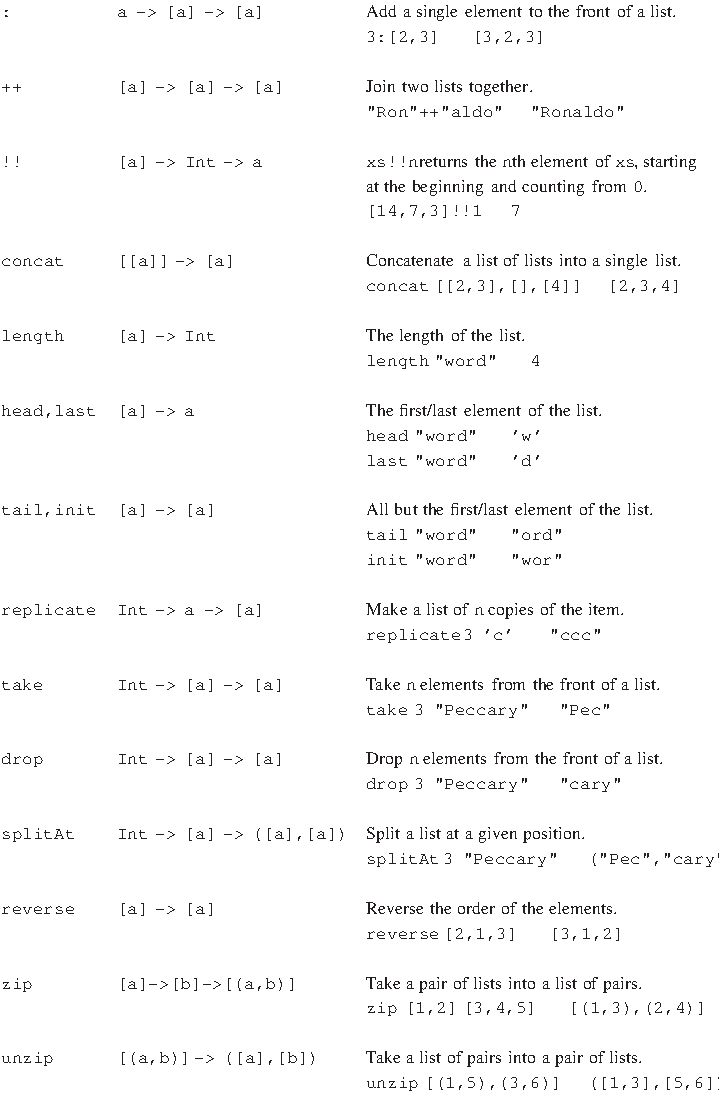
\includegraphics{Pictures/fig5-1.pdf}
\caption{Some polymorphic list operations from \texttt{Prelude.hs}.}
\label{polyListOps}\index{Peccary, Greggery}\index{Greggery Peccary|see{Peccary, Greggery}}
\end{figure}

Armed with the insight provided by the
previous section we can look at the descriptions of the polymorphic list
operations from \texttt{Prelude} given in Figure \ref{polyListOps}. 
In this table we give the name of the
function or operator, its type, a brief description of its effect and an
example, as in the description of \texttt{length}\minx{length}
\begin{center}
\begin{tabular}{>{\ttfamily}p{0.7in}>{\ttfamily}p{1.5in}>{\setlength{\rightskip}{0pt plus 1fil}}p{2.5in}}
length & [a] -> Int & The length of the list.\\
&& \texttt{length "word" \step 4}
\end{tabular}
\end{center}

As well as the polymorphic functions in Figure \ref{polyListOps}, the
standard prelude provides various operations over specific types; some
of these can be seen in Figure \ref{monoListOps}. The types of the
functions
\texttt{sum} and \texttt{product}, which are overloaded, 
will be discussed further in Chapter \ref{typeClasses}.

\begin{figure}
\begin{center}\minx{sum}\minx{product}\minx{and}\minx{or}
\begin{tabular}{>{\ttfamily}p{0.7in}>{\ttfamily}p{1.3in}>{\setlength{\rightskip}{0pt plus
1fil}}p{2.5in}} and & [Bool] -> Bool & The conjunction of a list of Booleans.\\
&& \texttt{and [True,False] \step False}\\ \\
or & [Bool] -> Bool & The disjunction of a list of
Booleans.\\
&& \texttt{or [True,False] \step True}\\ \\
sum & [Integer] -> Integer & The sum of a numeric list.\\
 & [Float] -> Float & \texttt{sum [2,3,4] \step 9}\\ \\
product & [Integer] -> Integer & The product of a numeric list.\\
 & [Float] -> Float & \texttt{product [0.1,0.4 ..\ 1] \step 0.028}
\end{tabular}
\end{center}
\vspace{-10pt}
\caption{Some monomorphic list operations from the \texttt{Prelude}.}
\label{monoListOps}
\vspace{-6pt}
\end{figure}



\subsection*{The importance of types}
\index{type!importance of types}

The single most useful piece of information about a function is its
\textbf{type}, and this is particularly true when we look at the polymorphic types
of functions in a library like Figure \ref{polyListOps}. Suppose we are
looking for a function to make a list from a number of copies of a single element.
It must take the item and a count and give a list, so its type will be 
one of 
\begin{alltt}
Integer -> a -> [a]             a -> Integer -> [a]
\end{alltt}
Looking at Figure \ref{polyListOps} we can quickly locate 
one function, \texttt{replicate}, which does have one of
these types and is indeed the function which we seek. If we want a
function to reverse a list it will have type \mbox{\texttt{[a] -> [a]}} and
although there is more than one function with this type, the search is
very much narrowed by looking at types. We'll see a little later on (page \pageref{hoogle}) that there's a web service called \emph{{hoogle}} to look up functions by type.

This insight is not confined to functional languages, but is of
particular use when a language supports polymorphic or \textbf{generic}
functions and operators as we have seen here.

\subsection*{Further functions}

We have not described all the functions in the prelude for two different
reasons. First, some of the general functions are \textbf{higher-order}
and we postpone discussion of these until Chapter \ref{patternsGen}; secondly,
some of the functions, such as \texttt{zip3}, are obvious variants of
things we have discussed here. Similarly, we have not chosen to
enumerate the functions in the library \texttt{Data.List}; \minx{Data.List}readers should
consult the library file itself, which contains type information and comments
about the effects of the functions, as well as the Haddock documentation for the library: we talk in detail about documentation in the next section.

\begin{figure}[t]
\begin{center}
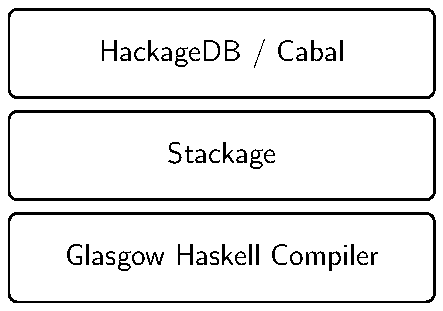
\includegraphics[width=3in]{Pictures/Infrastructure.pdf}
\end{center}
\caption{The Haskell infrastructure}
\label{HaskellInfrastr}
\end{figure}

\index{lists!prelude functions|)}


\section{Finding your way around the Haskell libraries}
\label{HaskellLibs}\index{libraries, finding your way around|(}

\begin{figure}[t]
\beware{A note on \texttt{module} names and exports}{\label{note-names}\index{modules!hierarchical names}\index{pitfalls!module names}
Module names in Haskell 2010 are ``hierarchical'' in style, and consist of a sequence of identifiers beginning with capital letters, separated with dots. Examples in the standard libraries include \texttt{Foreign.Marshal.Alloc}, \texttt{Data.Bool} and \texttt{Foreign}.
To quote from the report 
\begin{quote}
Module names can be thought of as being arranged in a hierarchy in which appending a new component creates a child of the original module name. For example, the module \texttt{Control.Monad.ST} is a child of the \texttt{Control.Monad} sub-hierarchy. This is purely a convention, however, and not part of the language definition.
\end{quote}
However, that's not quite the end of the story, because some modules are defined in such a way as to (re-)export all their ``children'': an example of this is the module \texttt{Foreign.C} (quoting again from the report)
\begin{quote}
The module \texttt{Foreign.C} combines the interfaces of all modules providing C-specific marshalling support, namely
\begin{alltt}
module Foreign.C.Types 

module Foreign.C.String 

module Foreign.C.Error
\end{alltt}
\end{quote}
while other modules export a subset of that functionality:
\begin{quote}
The module \texttt{Foreign} combines the interfaces of all modules providing language-independent marshalling support, namely
\begin{alltt}
module Data.Bits 

module Foreign.Ptr 

 ...
\end{alltt}
\end{quote}
}
\end{figure}

\begin{figure}[t]
\beware{Packages and Hackage}{\label{package-hackage}\index{HackageDB}\index{package}
\textbf{Hackage} is the standard online repository for Haskell code, bundled up as \textbf{packages}. The simplest package is a collection of Haskell modules, but more complex packages can contain C code, documentation, test cases and so on. Hackage keeps track of dependencies between packages, including which versions of each dependency a package is compatible with.

Combined with Cabal\index{Cabal}, this gives a straightforward way to download and maintain sets of Haskell libraries. Cabal has facilities for package developers and maintainers too, but we confine ourselves to user-facing features here.

\medskip
\textbf{Packages} have a globally unique \textbf{package name} and a \textbf{version number}, such as \texttt{mypackage-1.4.2}. Each package will \textbf{expose} some of the Haskell modules it contains. Crucially, the package will state which other packages it depends on, typically in as general as possible a way: a dependency such as \texttt{base >=4.14 \&\& <5} lets the package use any version of \texttt{base} in that range. Further details of how packages are described is available at the Hackage website, \url{https://hackage.haskell.org/}.
A typical package description page on Hackage is shown in Figure \ref{HackagePic}.
}
\end{figure}

\begin{figure}[t]
\beware{Cabal}{\label{cabal}\index{Cabal}
\textbf{Cabal} is the standard command-line tool for building Haskell projects and for installing packages -- and whatever they depend on -- on your system. It is installed automatically by GHCup\index{GHCup} alongside GHC itself, as described in Chapter \ref{getStart}. Day to day, working on this book's own code, you mainly need \texttt{cabal build} and \texttt{cabal repl}, described in Section \ref{multipleModuleProgs}, which build a project and its dependencies and open a GHCi session connected to them respectively: Cabal works out for itself, from the project's \texttt{.cabal} file, which packages need to be fetched and built.

For working with packages more generally these further commands are useful.
\begin{description}\index{Cabal!\texttt{cabal} commands}
\item{\mbox{\texttt{cabal update}}}
\\Refresh the local, cached list of packages available on Hackage. It's sensible to do this occasionally.
\item{\mbox{\texttt{cabal list string}}}
\\List all the packages whose descriptions contain a match of the \texttt{string}; all packages are listed if the string is omitted.
\item{\mbox{\texttt{cabal install pkg}}}
\\Install \texttt{pkg} as a standalone executable, so that it's available on the command line; add \texttt{-{}-lib} instead to make a package available as a library outside of any particular project.
\item{\mbox{\texttt{cabal install 'pkg < 2'}}}
\\Install a version of \texttt{pkg} with a constrained version number.
\item{\mbox{\texttt{cabal install pkg -{}-dry-run}}}
\\Dry run what happens if you install a particular \texttt{pkg}.
\item{\mbox{\texttt{cabal help}}}
\\Give a summary of all the available cabal commands.
\item{\mbox{\texttt{ghc-pkg list}}}\minx{ghc-pkg}
\\List all the packages currently visible to GHC.
\end{description}
Full documentation for Cabal is available at \url{https://cabal.readthedocs.io/}.
}
\end{figure}



Haskell comes with some great libraries which will allow you to get started writing programs in all sorts of different application areas without having to build up everything from scratch yourself, thanks to the contributions of thousands of people in the Haskell community.

\subsection*{What libraries are there?}

Libraries are found in the Haskell 2010 standard, including the \texttt{Prelude}, in curated distributions such as Stackage, and on the Hackage database.
We first describe the libraries in some more detail, and then explain how to find out more about them.


\begin{description}
\item[Prelude] 
The \texttt{Prelude} is a part of the language standard and gives definitions of standard types, functions and classes (which we come to later). The \texttt{Prelude} is listed in full in the Haskell 2010 Language Report.

The \texttt{Prelude} is special because it is imported into all modules by default. We have seen this already: if we want to re-define a \texttt{Prelude} function, then we have to import the \texttt{Prelude} explicitly, but \texttt{hiding} that function.

\item[Haskell 2010]\index{Haskell 2010} 
The standard libraries in Haskell 2010 use hierarchical names: see the note on module names on page \pageref{note-names} for more details of this. 

The libraries are grouped by name, and are described in depth in the Haskell 2010 Language Report:
\begin{description}
\item[Control]\minx{Control}
The \texttt{Control.Monad} library contains definitions which underly the IO mechanism in Haskell, as well as structuring side-effecting computations and DSL definitions.
\item[Data]\minx{Data}
These libraries contain additional data types, e.g. \texttt{Data.Array}, or additional operations on existing types, such as the bitwise operations on integers in \texttt{Data.Bit}.
\item[Foreign]\minx{Foreign}
The \texttt{Foreign} libraries provide support for interworking with other programming languages. This includes support for the communication of data between languages in \texttt{Foreign.C} and \texttt{Foreign.Marshal}, as well as facilities for pointers to foreign entities.
\item[Numeric]\minx{Numeric}
The \texttt{Numeric} library contains functions to read and print numbers in a variety of formats.
\item[System]\minx{System}
The \texttt{System} libraries have support for various forms of IO handling (in \texttt{System.IO} and \texttt{System.IO.Error}), and functions to interact with the command line and signals in Unix.
\end{description}

\item[Stackage]\index{Stackage}
Beyond the standard libraries, the great majority of Haskell code lives in packages on Hackage (described next). Because anyone can upload a package, and packages can drift out of sync with each other's dependencies, \textbf{Stackage}, \url{https://www.stackage.org/}, curates \textbf{snapshots}: large sets of Hackage packages that are tested and known to build together, including both a frequently-updated \textbf{Nightly} snapshot and slower-moving, long-term-support (\textbf{LTS}) snapshots. Between packages installed directly via Cabal and packages taken from a Stackage snapshot, the areas covered include the following.
\begin{itemize}
\item
Data and control structures, such as sets, finite maps, bytestrings and hash tables.
\item
Concurrency, including lightweight threads, MVars for thread synchronisation and channels.
\item
Testing and debugging, including \texttt{HUnit} and \texttt{QuickCheck}, as we use here.
\item
Network, system and web programming, including facilities for HTTP and socket programming, as well as access to many OS-level and lower-level operations.
\item
Other packages cover text processing, graphics and mathematics.
\end{itemize}
\item[HackageDB]\index{HackageDB}
HackageDB provides an online repository for sharing and distributing Haskell packages and libraries. It has been running continuously since 2007, and now hosts tens of thousands of packages, a testament to the strength and engagement of the Haskell developer community. The variety and number of packages make it impossible to give a summary of what's there: you'll need to consult the documentation to find out more. We turn to looking at that now.
\end{description}
Figure \ref{HaskellInfrastr} illustrates the layers of libraries available.



\subsection*{Where do I find out more?}

You can find out about the Haskell libraries in a number of different places, some installed locally alongside GHC, and others online. Much of the online documentation is generated using the \textbf{Haddock}\index{Haddock} system, which is itself installed alongside GHC. Haddock documents are hyperlinked for ease of navigation, and also provide links from the documentation into the source code, so that you don't have to look at that separately.

We'll go through these in turn now.

\begin{figure}[t] 
\begin{center}
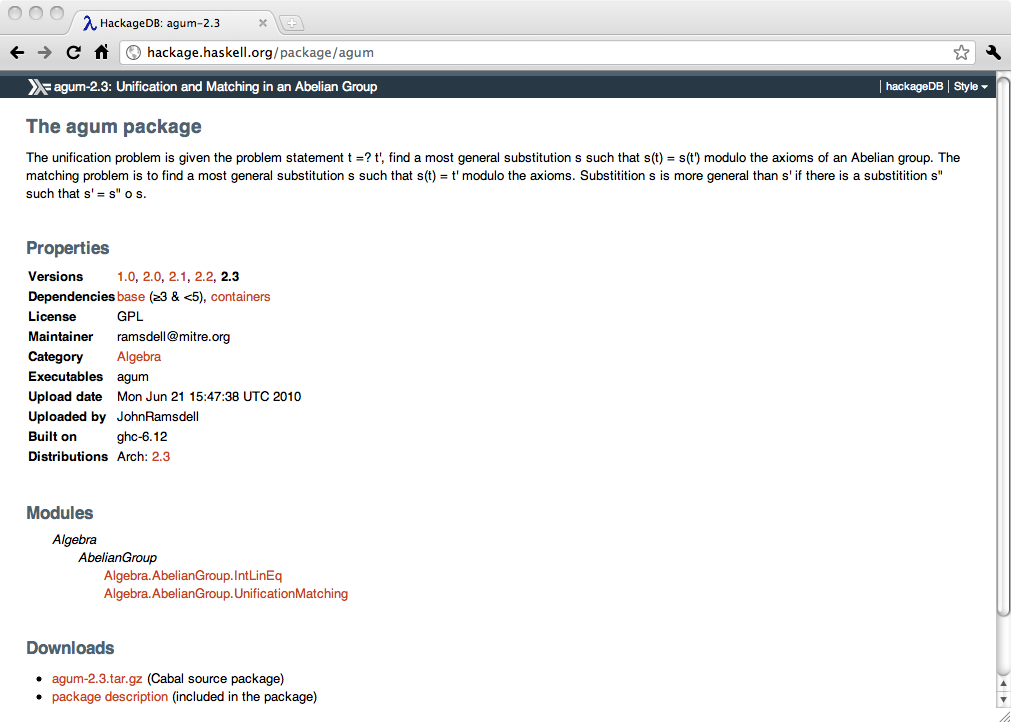
\includegraphics[width=12cm]{Pictures/HackagePic.png}
\end{center} 
\caption{The HackageDB description of the \texttt{accelerate} package}
\label{HackagePic}
\end{figure}

\begin{figure}[t] 
\begin{center}
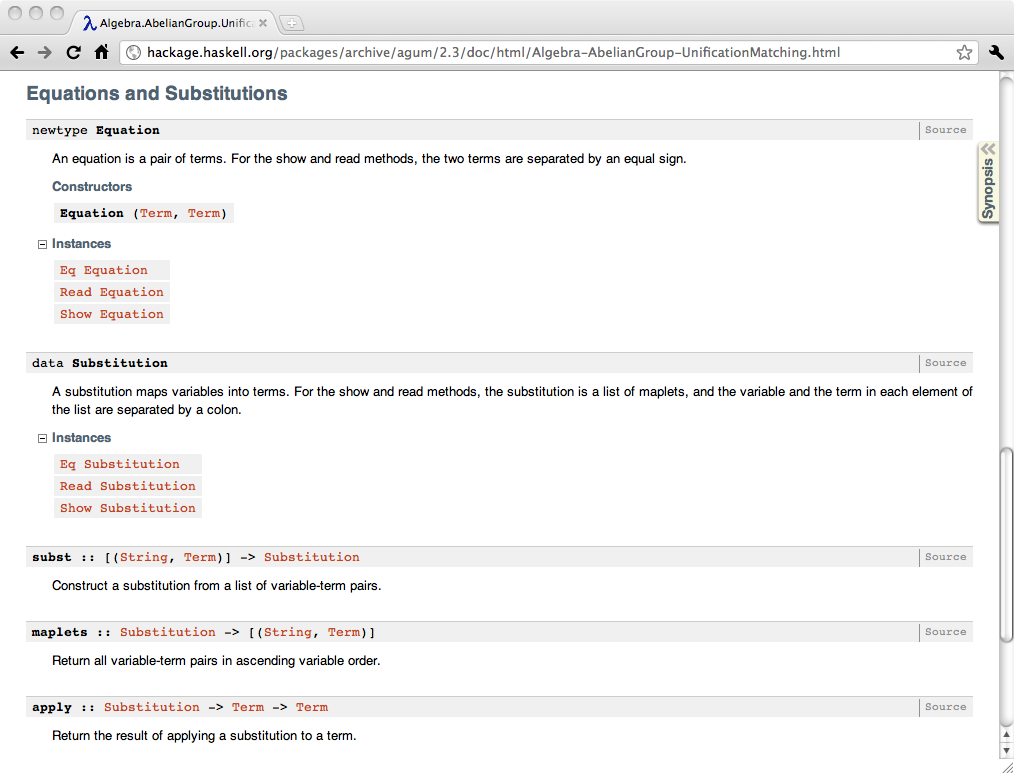
\includegraphics[width=12cm]{Pictures/HaddockPic.png}
\end{center} 
\caption{Haddock documentation for the \texttt{accelerate} package}
\label{Haddock}
\end{figure}


\begin{figure}[t] 
\begin{center}
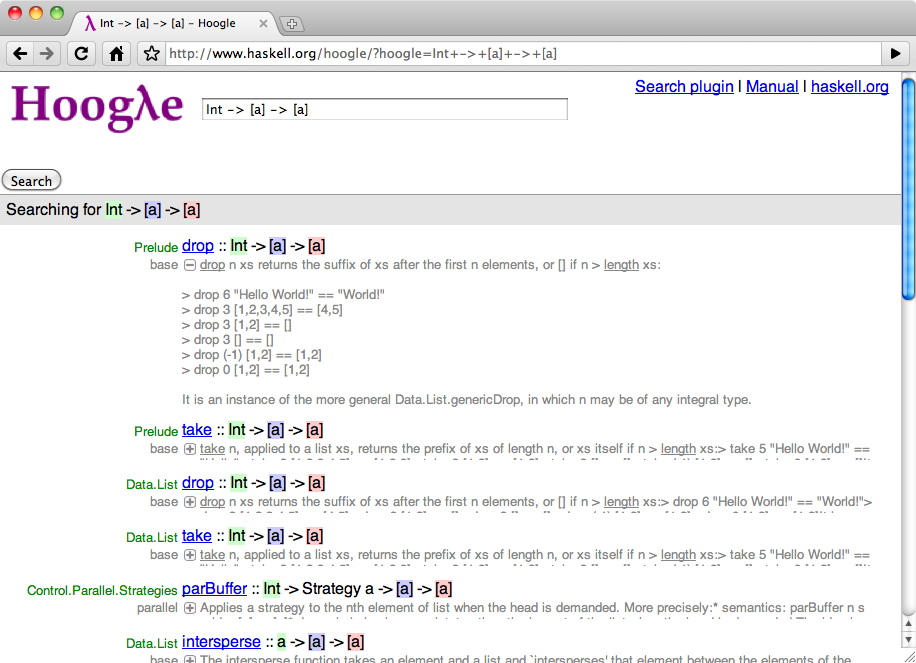
\includegraphics[width=12cm]{Pictures/Hoogle.png}
\end{center} 
\caption{Hoogle in action}
\label{Hoogle}
\end{figure}


\begin{description}
\item[System documentation]\index{documentation!system}
Once GHC is installed via GHCup\index{GHCup}, documentation for the compiler and the libraries that ship with it is also installed locally; GHCup's own documentation, \url{https://www.haskell.org/ghcup/}, explains where to find it on your platform. In practice, though, most readers find it quicker simply to use the online, Hackage-hosted documentation described below, which is always up to date and identical in content.
\item[Libraries]\index{documentation!libraries}
Haddock documentation for the libraries that ship with GHC -- \texttt{base}, \texttt{containers}, \texttt{bytestring} and so on -- is hosted on Hackage alongside everything else; see \textbf{Hackage}, below.
\item[Prelude]\index{documentation!prelude}
In particular, documentation for the \texttt{Prelude}, including descriptions of and examples for many of the functions, is part of the documentation for the \texttt{base} package, and is available directly at \url{https://hackage.haskell.org/package/base/docs/Prelude.html}, which always points to the documentation for whichever version of \texttt{base} ships with the current release of GHC.
\item[Hackage]\index{documentation!Hackage}
Haddock documentation is available for the great majority of packages on Hackage. This is accessible from \url{https://hackage.haskell.org/package/}, which is listed by category, but also searchable. A typical package page is shown in Figure \ref{HackagePic}: documentation for the modules making up the package is linked from the list of modules below the \textbf{Modules} header, towards the bottom of the page; an example is shown in Figure \ref{Haddock}.
\item[Hoogle search]\label{hoogle}\index{documentation!Hoogle}\index{Hoogle}
Hoogle allows you to search many of the standard and Hackage libraries: what is cool about Hoogle is that you can \textbf{search by type} as well as by name. Narrowing down a search by type can lead you very quickly to your answer, or at least eliminate a lot of ``noise'' in a search: \url{https://hoogle.haskell.org/}.
See Figure \ref{Hoogle} for example results. Be aware, though, that Hoogle doesn't cover every package on Hackage. A general web search -- even using a type signature as the search text -- is also often surprisingly effective.
\item[GHCi]\index{documentation!GHCi}\index{GHCi!documentation}
Once you have asked to \texttt{import} a module (\texttt{Foo}, say) into GHCi you can then find out the types of all its exported functions using the GHCi command
\begin{alltt}
:browse Foo
\end{alltt}
Information about a particular function (\texttt{foo}, say) which is in a module loaded in GHCi is given using the command
\begin{alltt} 
:info foo
\end{alltt}
\item[Online resources]
You can go online to ask questions. The Haskell Discourse, \url{https://discourse.haskell.org}, is now the liveliest general home for Haskell discussion and questions; the Haskell Cafe mailing list, \texttt{haskell-cafe@haskell.org}, IRC channels and Stack Overflow's \texttt{haskell} tag remain active too. Links to all of these can be found in the \textbf{Community} section of the Haskell website, \url{https://www.haskell.org}.
\item[Online texts]
Finally, you can find a number of texts online, including the community-maintained continuation of \emph{Learn You a Haskell for Great Good!}, \url{https://learnyouahaskell.github.io/}, and the \emph{Haskell wikibook}, \url{https://en.wikibooks.org/wiki/Haskell}.
\end{description}

\index{libraries, finding your way around|)}





\section{The \texttt{Picture} example: implementation}
\markright{The \texttt{\runinghead  Picture} example: implementation}
\label{picturesAgain}
\index{pictures|(}
\minx{Picture}

In this section we revisit the \texttt{Picture} example, first
introduced in Chapter \ref{intro} and re-examined in Section
\ref{picModuleEx}. What we do here is to look at how to implement
some of the operations over the \texttt{Picture} type, now that we know about list comprehensions and the list functions in the prelude. We also look at how to write more QuickCheck properties for the \texttt{Picture} functions.
\begin{alltt}
type Picture = [[Char]]
\end{alltt}
Some of the operations are defined as library functions. To flip a
picture in a horizontal mirror, we simply have to reverse the order of
the lines of the picture:
\begin{alltt}
flipH :: Picture -> Picture
flipH = reverse\minx{flipH}
\end{alltt}
and to place one picture above another it is sufficient to join the two lists of
lines together:
\begin{alltt}
above :: Picture -> Picture -> Picture
above = (++)\minx{above}
\end{alltt}
where we have enclosed the operator \texttt{++} in parentheses to make it 
a (prefix) function.

How do we flip a picture in a vertical mirror? We have to reverse each
of the lines, that is we have to transform each member of a list in some
way. This is one of the features of a list comprehension, so we can say
\begin{alltt}\index{list comprehensions}\minx{flipV}
flipV :: Picture -> Picture
flipV pic 
  = [ reverse line | line <- pic ]
\end{alltt}
and we can read off from this program its intended effect:
\begin{quote}
``\texttt{reverse} every \texttt{line} in the \texttt{pic}''.
\end{quote}
This is an example of the general operation of applying a function \texttt{f} to every 
element of a list \texttt{xs}, given by the list comprehension
\begin{alltt}
[ f x | x <- xs ]
\end{alltt}
We shall see that this operation is itself a higher-order function in
Chapter \ref{patternsGen} below.

Next we explore how to place two pictures side by side. What we want to
do is to join up the corresponding lines of the two pictures, as
illustrated on page \pageref{beside}. How can we accomplish this? We
can see this as like \texttt{flipV}, in that we want to do something to
every pair of lines -- namely join them with \texttt{++} -- 
but we need to associate corresponding lines before
we do this. That is exactly the purpose of the prelude
function \texttt{zip},\minx{zip} which takes two lists and
pairs corresponding elements, and so we can
say
\begin{alltt}\minx{beside}
beside :: Picture -> Picture -> Picture
beside picL picR
  = [ lineL ++ lineR | (lineL,lineR) <- zip picL picR ]
\end{alltt}
The effect of \texttt{zip} is to chop the list of pairs to the shorter
of the two inputs, and so \texttt{beside} will clip the bottom lines
off whichever picture is the longer; if they are the same length, then
there is no clipping. We can also use the higher-order \texttt{zipWith}
to define \texttt{beside}; we revisit this in Chapter~9.

In our pictures, white is represented by the dot `\texttt{.}' and black
by the hash symbol `\texttt{\#}'. To invert the colour of a single
character we define
\begin{alltt}\minx{invertChar}
invertChar :: Char -> Char
invertChar ch 
  = if ch=='.' then '\#' else '.'
\end{alltt}
The characters `\texttt{.}' and `\texttt{\#}' are swapped by this
definition (and any other character is transformed into `\texttt{.}',
too).
Now, how do we invert the colours in a whole picture? We need to invert
each character in a line, using  
\begin{alltt}\minx{invertLine}
invertLine :: [Char] -> [Char]
invertLine line 
  = [ invertChar ch | ch <- line ]
\end{alltt}
and we want to apply this to all the lines in the picture
\begin{alltt}\minx{invertColour}
invertColour :: Picture -> Picture
invertColour pic 
  = [ invertLine line | line <- pic ]
\end{alltt}
We could if we wish write this as a single definition, thus
\begin{alltt}
invertColour :: Picture -> Picture
invertColour pic 
  = [ [ invertChar ch | ch <- line ] | line <- pic ]
\end{alltt}
but our use of the auxiliary function \texttt{invertLine} makes the
previous
definition more readable.

In the next section we extend our model of pictures to give them a position as well
as some pictorial content.


\subsection*{Tests and properties}

We first discussed writing properties for the functions over pictures in Section \ref{pictureProps}; it's time to look at this again. In that section we looked at properties  of \texttt{flipH} and \texttt{flipV}, separately and together. Here we look at how these functions interact with \texttt{above} and \texttt{beside}, and we look at other properties in the exercises.\index{QuickCheck!pictures}

What happens if we flip \texttt{pic1 `above` pic2} in a vertical mirror? The result is the same as flipping the two pictures separately before putting them together. We can write this as a property
\begin{alltt}\minx{prop\_AboveFlipV}
prop_AboveFlipV :: Picture -> Picture -> Bool

prop_AboveFlipV pic1 pic2 = 
    flipV (pic1 `above` pic2) == (flipV pic1) `above` (flipV pic2) 
\end{alltt}
and test it by typing
\begin{alltt}
quickCheck prop_AboveFlipV
\end{alltt}
(ensuring that the module \texttt{Test.QuickCheck} is loaded.) Similarly we can write the property for \texttt{flipH}:
\begin{alltt}\minx{prop\_AboveFlipH}
prop_AboveFlipH :: Picture -> Picture -> Bool

prop_AboveFlipH pic1 pic2 = 
    flipH (pic1 `above` pic2) == (flipH pic1) `above` (flipH pic2) 
\end{alltt}
but this fails: why? Can you correct the property? Remember that \texttt{flipH} means that we're flipping the picture in a \emph{horizontal} mirror.

In Section \ref{localDefs} we put together four pictures as \texttt{fourPics}. We chose to do this by putting one picture beside another using \texttt{beside}: we could also have done this by putting one picture \texttt{above} another, and we could expect that this gives the same result, as expressed in the property
\begin{alltt}
propAboveBeside :: Picture -> Picture ->  Picture -> Picture -> Bool

propAboveBeside nw ne sw se =
  (nw `beside` ne) `above` (sw `beside` se) 
  == 
  (nw `above` sw) `beside` (ne `above` se) 
\end{alltt}
If we test this, then it fails. Why? Remember that we're using the built-in facilities of QuickCheck to generate \emph{random} values from \texttt{[String]}. If we look at a sample of the data,\footnote{We do this using\ \ \texttt{sample (arbitrary ::\ Gen\  [String]).}} the results look like this:
\begin{alltt}
[]
["a1","\bs{}EOT"]
[]
["","p\bs{}DC3=","\bs{}229\bs{}a\bs{}183","\bs{}218\bs{}SOH\bs{}194",""]
["g\}","P","_y","\bs{}169\bs{}131\bs{}FS\bs{}t","U\bs{}nl",":YicLX\bs{}194\bs{}198","\bs{}t3"] 
 \ldots
\end{alltt}
The elements are random, the pictures are generally not rectangular -- because within each list the strings are of different length -- it is also very likely that four of these chosen randomly will not have the right dimensions to be put together using \texttt{beside} and \texttt{above}. We'll see in Section \ref{qcGens} how to define random \emph{generators} of data for ourselves, and we'll see there how to generate `sensible' random pictures, built up from \texttt{'.'} and \texttt{'\#'} in rectangular patterns, and indeed to generate sets of pictures containing random data but all of the same size.

In the meantime we can say that we only want to check a property when the generated data  satisfy some conditions: let's take a look at an example.
\begin{alltt}
propAboveBeside3Correct :: Picture -> Picture -> Property

propAboveBeside3Correct w e =
  (rectangular w && rectangular e && height w == height e) 
  ==>
     (w `beside` e) `above` (w `beside` e) 
         == 
     (w `above` w) `beside` (e `above` e) 
\end{alltt}
In writing this property we have used \texttt{==>} which we can read as `implies'. 
The property following the \texttt{==>} is only checked when the \texttt{Bool}ean \emph{condition} before the arrow is true. Without the condition the property fails: try it out! 









\begin{exercises}


\item
Define a function
\begin{alltt}
superimposeChar :: Char -> Char -> Char
\end{alltt}
so that the superimposition of `\texttt{.}' with itself gives
`\texttt{.}' while any other combination of characters gives
`\texttt{\#}'.

\item
Define a function
\begin{alltt}
superimposeLine :: [Char] -> [Char] -> [Char]
\end{alltt}
which takes two lines -- which you can assume are of the same length --
and superimposes their corresponding characters using \texttt{superimposeChar}, so that, for example,
\begin{alltt}
superimposeLine ".##." ".#.#" = ".###"
\end{alltt}
You may want to use \texttt{zip} in your solution.

\item
In a similar way to \texttt{superimposeLine},
define the function
\begin{alltt}\minx{superimpose}
superimpose :: Picture -> Picture -> Picture
\end{alltt}
which superimposes two pictures, which you may assume have the same
dimensions. 

\item
Using the function 
\texttt{putStr ::\ String -> IO ()}
and any other functions you might need, define the function 
\begin{alltt}\minx{printPicture}
printPicture :: Picture -> IO ()
\end{alltt}
so that the effect of 
\texttt{printPicture [\,".\#\#."\,, ".\#.\#"\,, ".\#\#\#"\,, "\#\#\#\#"\,]}
is that
\begin{alltt}
.##.
.#.#
.###
####
\end{alltt}
is printed at the terminal window. \emph{Hint:} it is enough to transform this list of strings to the single string
\begin{alltt}
".\#\#.\bs{}n.\#.\#\bs{}n.\#\#\#\bs{}n\#\#\#\#\bs{}n"
\end{alltt}
and to pass that to \texttt{putStr}.


\item {[Harder]} 
Define a function
\begin{alltt}
rotate90 :: Picture -> Picture
\end{alltt}\minx{rotate90}
which rotates a picture through $90^\circ$ clockwise. For
instance, the effect of \texttt{rotate90} on the picture in the previous exercise
would be to give
\begin{alltt}
#...
####
##.#
###.
\end{alltt} 
Hint: you need to make a line of the new picture by picking out the
\texttt{i}th elements in each of the lines of the original picture, reflected 
in a horizontal mirror. 

\item
Using \texttt{rotate90} or otherwise, define a function which rotates a picture through
$90^\circ$ {\em anti}clockwise.

\item
{[Harder]} Define the function
\begin{alltt}\index{scale@\texttt{scale}}
scale :: Picture -> Int -> Picture
\end{alltt}
which scales the input picture by the integer provided as the second
argument. For instance, if \texttt{exPic} is the picture
\begin{alltt}
#.#
..#
\end{alltt}
then the result of \texttt{scale exPic 2} should be
\begin{alltt}
##..##
##..##
....##
....##
\end{alltt}
In the case of a zero or negative scale factor, you should
return an empty picture.


\item
Correct the property \texttt{prop\_AboveFlipH} given earlier.

\item
Define properties which describe how \texttt{beside} interacts with \texttt{flipH} and \texttt{flipV}.

\item
One property we can show holds is that if we take the same picture and put four copies of it together using \texttt{beside} and \texttt{above} in the two different ways, then the results are the same. Express this as a quick check property.

\item
You can test your implementation of \texttt{rotate90} using QuickCheck. Can you think of properties which only use \texttt{rotate90} and others that use \texttt{rotate}? You may want to impose a condition that any picture involved is rectangular: the function is given in the program code for this chapter.

\item
What property would you expect \texttt{invertColour} to have? Can you be sure that this will hold for randomly generated data?

\item {[Harder]}
Write the analogue of \texttt{propAboveBeside3Correct} where two pictures are again used, but with two the same at the top (call them \texttt{n}) and two the same at the bottom (\texttt{s}, say). Do you need the condition in this case?







\end{exercises}
 




\section{Extended exercise: alternative implementations of pictures}
\label{aliterPictures}
\index{extended exercise!picture implementations|(}


This section looks again at the pictures example, and explores alternative implementations. First we look at extending the implementation so that two pictures don't have to be of compatible size when joining them together into one. After that we look at various alternative implementations of pictures as lists.

\subsection*{Incompatible combinations}

In earlier discussions of the \texttt{Picture} type, we have made the assumption that binary functions like \texttt{above} have been called on arguments of compatible size: in the case of \texttt{above} this would mean that the \emph{width} of the two arguments was the same. What should be done if this is not the case? 

We could reasonably assume that each picture was \emph{rectangular} and define the functions so that this \emph{invariant} was preserved by the binary functions. In the example of \texttt{above} this requires that pictures can be padded in an appropriate way. Let's take the specific example of 
\begin{alltt}
(horse `beside` horse)
       `above`
horse
\end{alltt}
as shown in Figure \ref{lshapedhorses}.
\begin{figure}[t]
\begin{center}
\begin{alltt}
.......##..........##...
.....##..#.......##..#..
...##.....#....##.....#.
..#.......#...#.......#.
..#...#...#...#...#...#.
..#...###.#...#...###.#.
.#....#..##..#....#..##.
..#...#.......#...#.....
...#...#.......#...#....
....#..#........#..#....
.....#.#.........#.#....
......##..........##....
.......##...
.....##..#..
...##.....#.
..#.......#.
..#...#...#.
..#...###.#.
.#....#..##.
..#...#.....
...#...#....
....#..#....
.....#.#....
......##....
\end{alltt}
\end{center}
\caption{`Ragged' picture}
\label{lshapedhorses}
\end{figure}
To preserve the rectangular picture, we need to pad out the lower as shown in Figure \ref{paddedhorses}.
\begin{figure}[t]
\begin{center}
\begin{alltt}
.......##..........##...
.....##..#.......##..#..
...##.....#....##.....#.
..#.......#...#.......#.
..#...#...#...#...#...#.
..#...###.#...#...###.#.
.#....#..##..#....#..##.
..#...#.......#...#.....
...#...#.......#...#....
....#..#........#..#....
.....#.#.........#.#....
......##..........##....
.......##...............
.....##..#..............
...##.....#.............
..#.......#.............
..#...#...#.............
..#...###.#.............
.#....#..##.............
..#...#.................
...#...#................
....#..#................
.....#.#................
......##................
\end{alltt}
\end{center}
\caption{``Padded' picture}
\label{paddedhorses}
\end{figure}

\begin{exercises}

\item
Redefine the functions over pictures to pad pictures in the way just described. One way to solve the problem is to use the function
\begin{alltt}
replicate :: Int -> a -> [a]
\end{alltt}
\texttt{replicate n x} returns a list containing \texttt{n} \texttt{x}s, so \texttt{replicate 3 'g'} is \texttt{"ggg"}.

\item
How would you work with basic pictures that were not rectangular? Define a function which will take a picture - as a list of \texttt{String}s -- and return a rectangular list of strings, padding out each line as necessary. Once you start with rectangular pictures the functions you defined in the first part of this exercise should be enough to preserve them as rectangular.
\end{exercises}

\subsection*{Alternative representations}

In this section we look at a number of different ways that these "low fi" pictures can be represented.


\begin{exercises}


\item
An alternative representation of \texttt{Picture} is the type
\begin{alltt}\index{pictures!alternative representation of}
[[Bool]]
\end{alltt}
where \texttt{True}
and \texttt{False} represent black and white points in a picture. How
would you have to modify the functions working over \texttt{Picture} to
accommodate this change? What are the advantages and disadvantages of
the two representations?


\item
We have represented pictures as a list of rows: how would you redefine the functions working over pictures if they are represented as a \emph{list of columns}. 

\item {[Harder]}
How would you re-implement the function \texttt{printPicture}, defined in the solution to exercise 6.7, so that it works over this column-based representation?

\item
It would be possible to represent a \texttt{Picture} as \emph{a single list of characters}, with \texttt{'\bs{}n'} terminating each line of the picture, as in
\begin{alltt}
".\#\#.\bs{}n.\#.\#\bs{}n.\#\#\#\bs{}n\#\#\#\#\bs{}n"
\end{alltt}
How would you redefine the picture manipulating functions over this representation? Which functions become easier to define? Which more difficult?

\end{exercises}

\subsection*{Run-length encoding}\index{run-length encoding}

A more compact representation is given by run-length encoding of Pictures, which will code a repeated character \emph{run} like \texttt{"\#\#\#"} as a pair, \texttt{(3,'\#')}, and a picture is represented as a member of \texttt{[[(Int,Char)]]}. For example, the picture
\begin{alltt}
.##.
.#.#
.###
####
\end{alltt}
is represented like this
\begin{alltt}
[ [(1,'.'), (2,'#'), (1,'.')],
  [(1,'.'), (1,'#'), (1,'.'), (1,'#')],
  [(1,'.'), (3,'#')],
  [(4,'#')] ]
\end{alltt}
using run-length encoding for each row of the picture.

\begin{exercises}

\item
Re-implement the functions over pictures to work with this new representation. In particular, how would you print pictures which were represented in this way?

\item
Is it the case that all your answers to the last question give the most compact representation, so that you don't have adjacent runs of the same character, as in 
\begin{alltt}
[(1,'.'), (2,'.'), (1,'#')]
\end{alltt}
which could be given more compactly as
\begin{alltt}
[(3,'.'), (1,'#')]
\end{alltt}
If this can happen with your functions, how could you change your definitions to avoid it?

\item
Take another look at the QuickCheck properties you wrote to test pictures: rewrite these for your alternative implementations. How many of the properties carry over to the alternative implementations without alteration, and how many have to be modified in some way?

\item {[Harder]}
The run-length encoding above works a line at a time, but it would be possible to give a more compact representation which combines runs in different lines. The earlier example could then be given by 
\begin{alltt}
[(1,'.'), (2,'#'), (2,'.'),
 (1,'#'), (1,'.'), (1,'#'),
 (1,'.'), (7,'#')]
\end{alltt}
This representation loses the length of the rows, so you would have to keep information about the row length in the type too, giving
\begin{alltt}
type Picture = (Int, [(Int,Char)] )
\end{alltt}
as the representation. Re-implement the picture functions to work over this type.

\item {[Harder]}
If you know that only the characters \texttt{'.'} and \texttt{'\#'} are used in a picture, how could you make the representation of the previous question even more compact?

\item {[Harder]}
Define two more representations of pictures yourself, and re-implement the picture functions over these types.



\end{exercises}

\index{extended exercise!picture implementations|)}




\section{Extended exercise: positioned pictures}
\label{posPix}
\index{extended exercise!positioned pictures|(}

The pictures that we have modelled using the type \texttt{Picture} are not
anchored at any particular point in space: 
we can think of them concretely as being on pieces of
paper which can be joined together, superimposed, rotated and so on.

A different model of pictures gives each picture a \texttt{Position}\minx{Position} in
space: we can then think of moving these pictures, of superimposing
two of these pictures to give another picture, and so on.
\begin{figure}[t]
\begin{center}
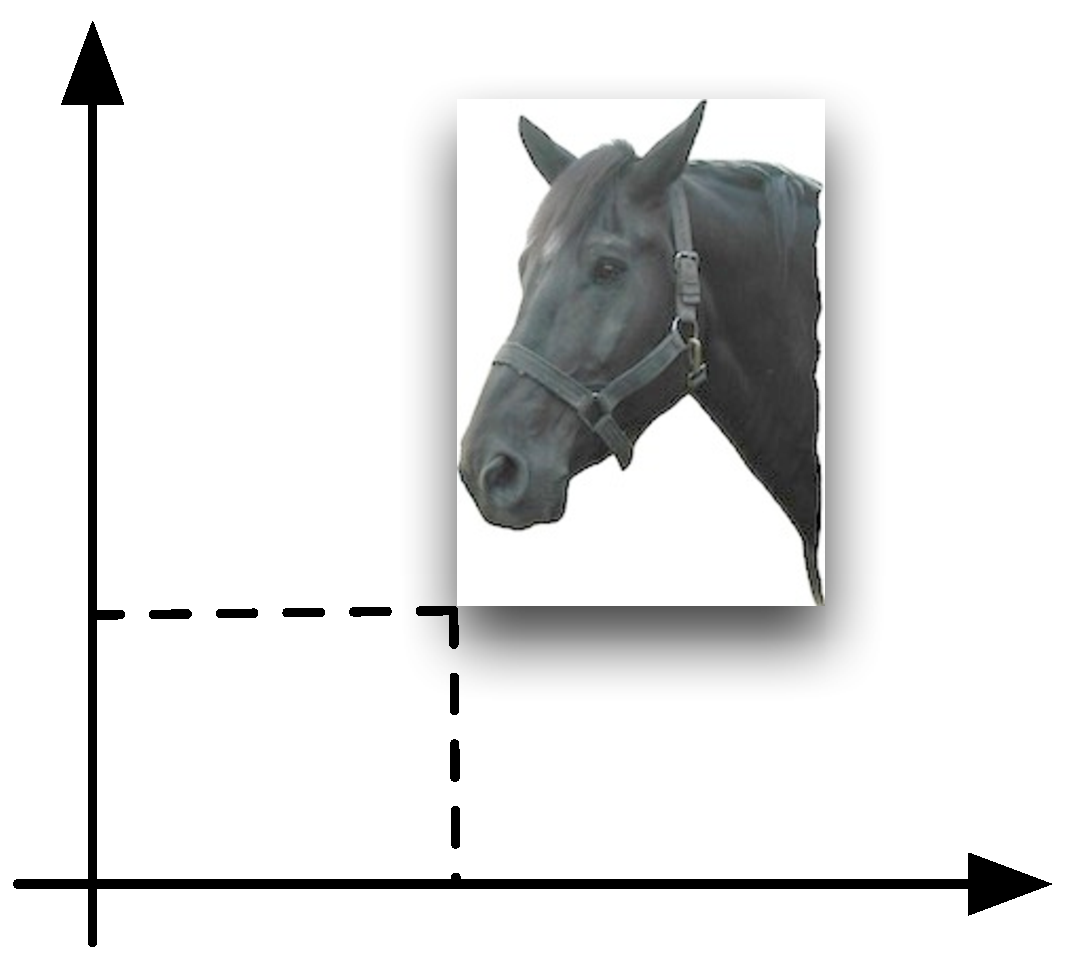
\includegraphics[width=2.5in]{Pictures/horsePos.pdf}
\end{center}
\caption{An example \texttt{Image}.\label{horsePos}}
\end{figure}

\subsection*{Basics}

How can we represent pictures with positions? First we need to
think about how we model positions on an {\em integer\/}
grid. A \texttt{Position} is given by a pair of integers,
\begin{alltt}
type Position = (Int,Int)
\end{alltt}
We will use the term \texttt{Image} for a picture with a position, and
so we define
\begin{alltt}\minx{Image}
type Image = (Picture,Position)
\end{alltt}
An example, in which we position the \texttt{horse} with its bottom
left-hand corner or \textbf{reference point}\index{reference point} at 
position \texttt{(31,23)}, is given in Figure
\ref{horsePos}.

The remainder of this section is a collection of exercises to write functions
which manipulate these \texttt{Images}; you can use any of the list
functions introduced in the previous chapter and also the functions
over \texttt{Picture}
which we have already defined.

\begin{exercises}


\item
Define a function
\begin{alltt}\minx{makeImage}
makeImage :: Picture -> Position -> Image
\end{alltt}
which makes an \texttt{Image}
from a \texttt{Picture} and a \texttt{Position}.

\item
Define a function
\begin{alltt}\minx{changePosition}
changePosition :: Image -> Position -> Image
\end{alltt}
which takes an \texttt{Image}
and returns a new \texttt{Image} whose \texttt{Picture} is unchanged but whose \texttt{Position}
is given by the second argument to \texttt{changePosition}.

\item
Give a definition of the function
\begin{alltt}\minx{moveImage}
moveImage :: Image -> Int -> Int -> Image
\end{alltt}
so that the effect of \texttt{moveImage img xMove yMove} is to move \texttt{img}
by \texttt{xMove} in the horizontal (\texttt{x}) direction and by \texttt{yMove} in
the vertical (\texttt{y}) direction.

\item
Define a function
\begin{alltt}
printImage :: Image -> IO ()
\end{alltt}
whose action is the analogue of \texttt{printPicture} for pictures.

\begin{figure}[t]
\begin{center}
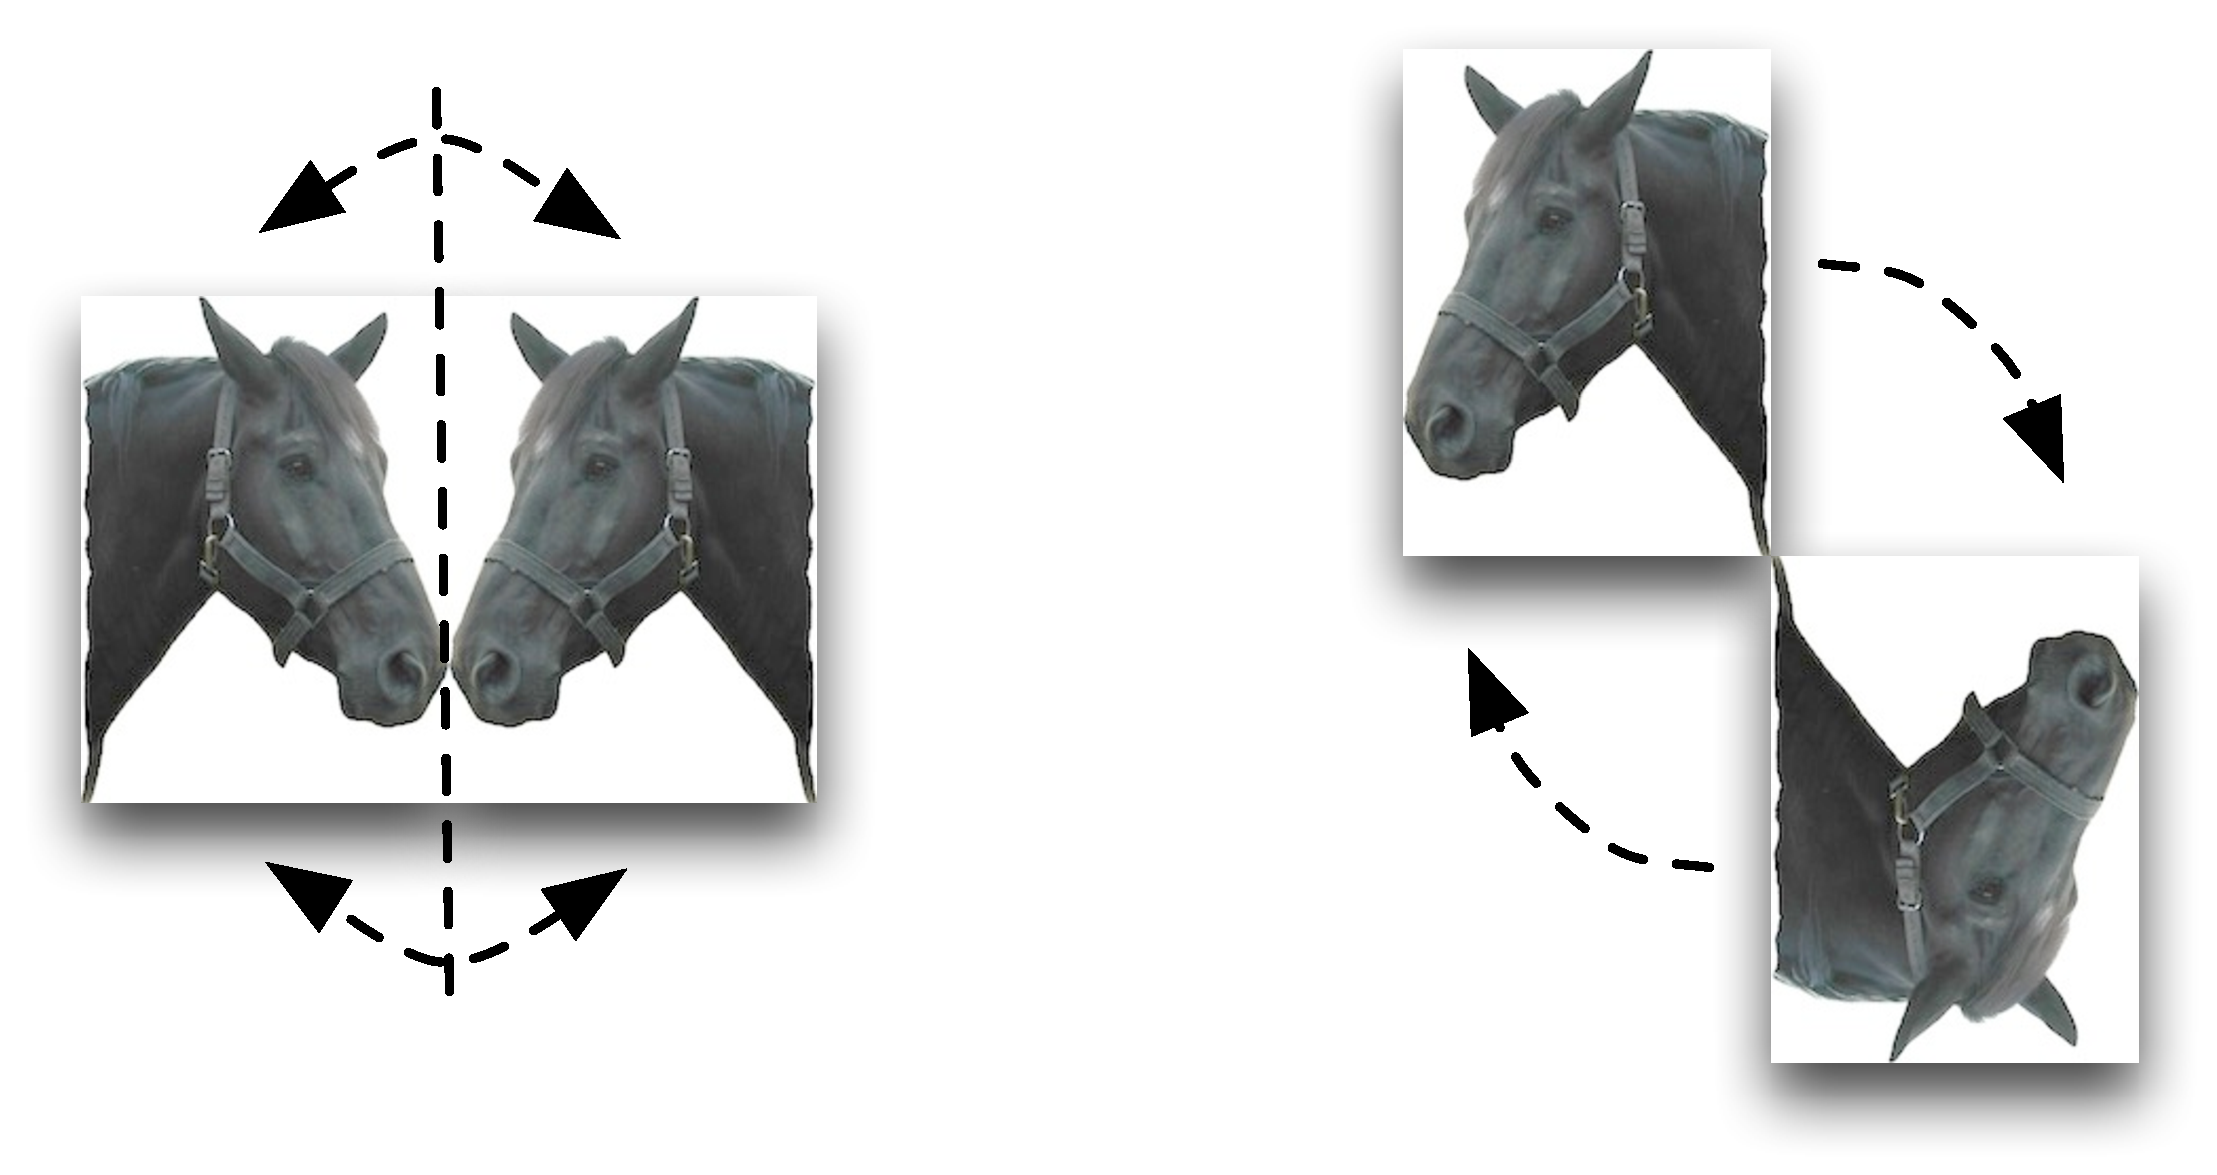
\includegraphics[width=4in]{Pictures/transfPos.pdf}
\end{center}
\caption{The geometrical view of \texttt{flipV} and \texttt{rotate}.}
\label{transfPos}
\end{figure}
\end{exercises}

\subsection*{Transformations}

We can extend the transformations over the type \texttt{Picture}
to the \texttt{Image} type, but we need to think about the effect of
these transformations on the position. One way to lift the
transformations from pictures to images
is simply to say that the pictures stay in the same
position -- we call this the \textbf{naive} view. 


If we think of reflections and rotations going on in space, then the
results are more likely to be as  shown in Figure \ref{transfPos},
where we see that the position of the resulting image has changed. Rotation is
about the reference point, and reflection is in the horizontal or vertical line through
the reference point; in general these operations will change the reference point. We
call this the \textbf{geometrical} view of the transformations. 

\begin{exercises}
\item
Implement for \texttt{Image} the analogues of \texttt{flipH}, \texttt{flipV},
\texttt{rotate} and \texttt{rotate90} under the naive view of how to lift the 
transformations.

\item
Implement for \texttt{Image} the analogues of \texttt{flipH}, \texttt{flipV},
\texttt{rotate} and \texttt{rotate90} under the geometrical view.
\end{exercises}

\subsection*{Superimposition}

When pictures have positions, superimposition can be more complex.
Consider the example illustrated in Figure \ref{superPos};
here we see one way of superimposing the two images is to use
\texttt{Picture} superimposition on two pictures which have first been
`padded out' with white space as shown in the figure. 

\begin{figure}[t]
\begin{center}
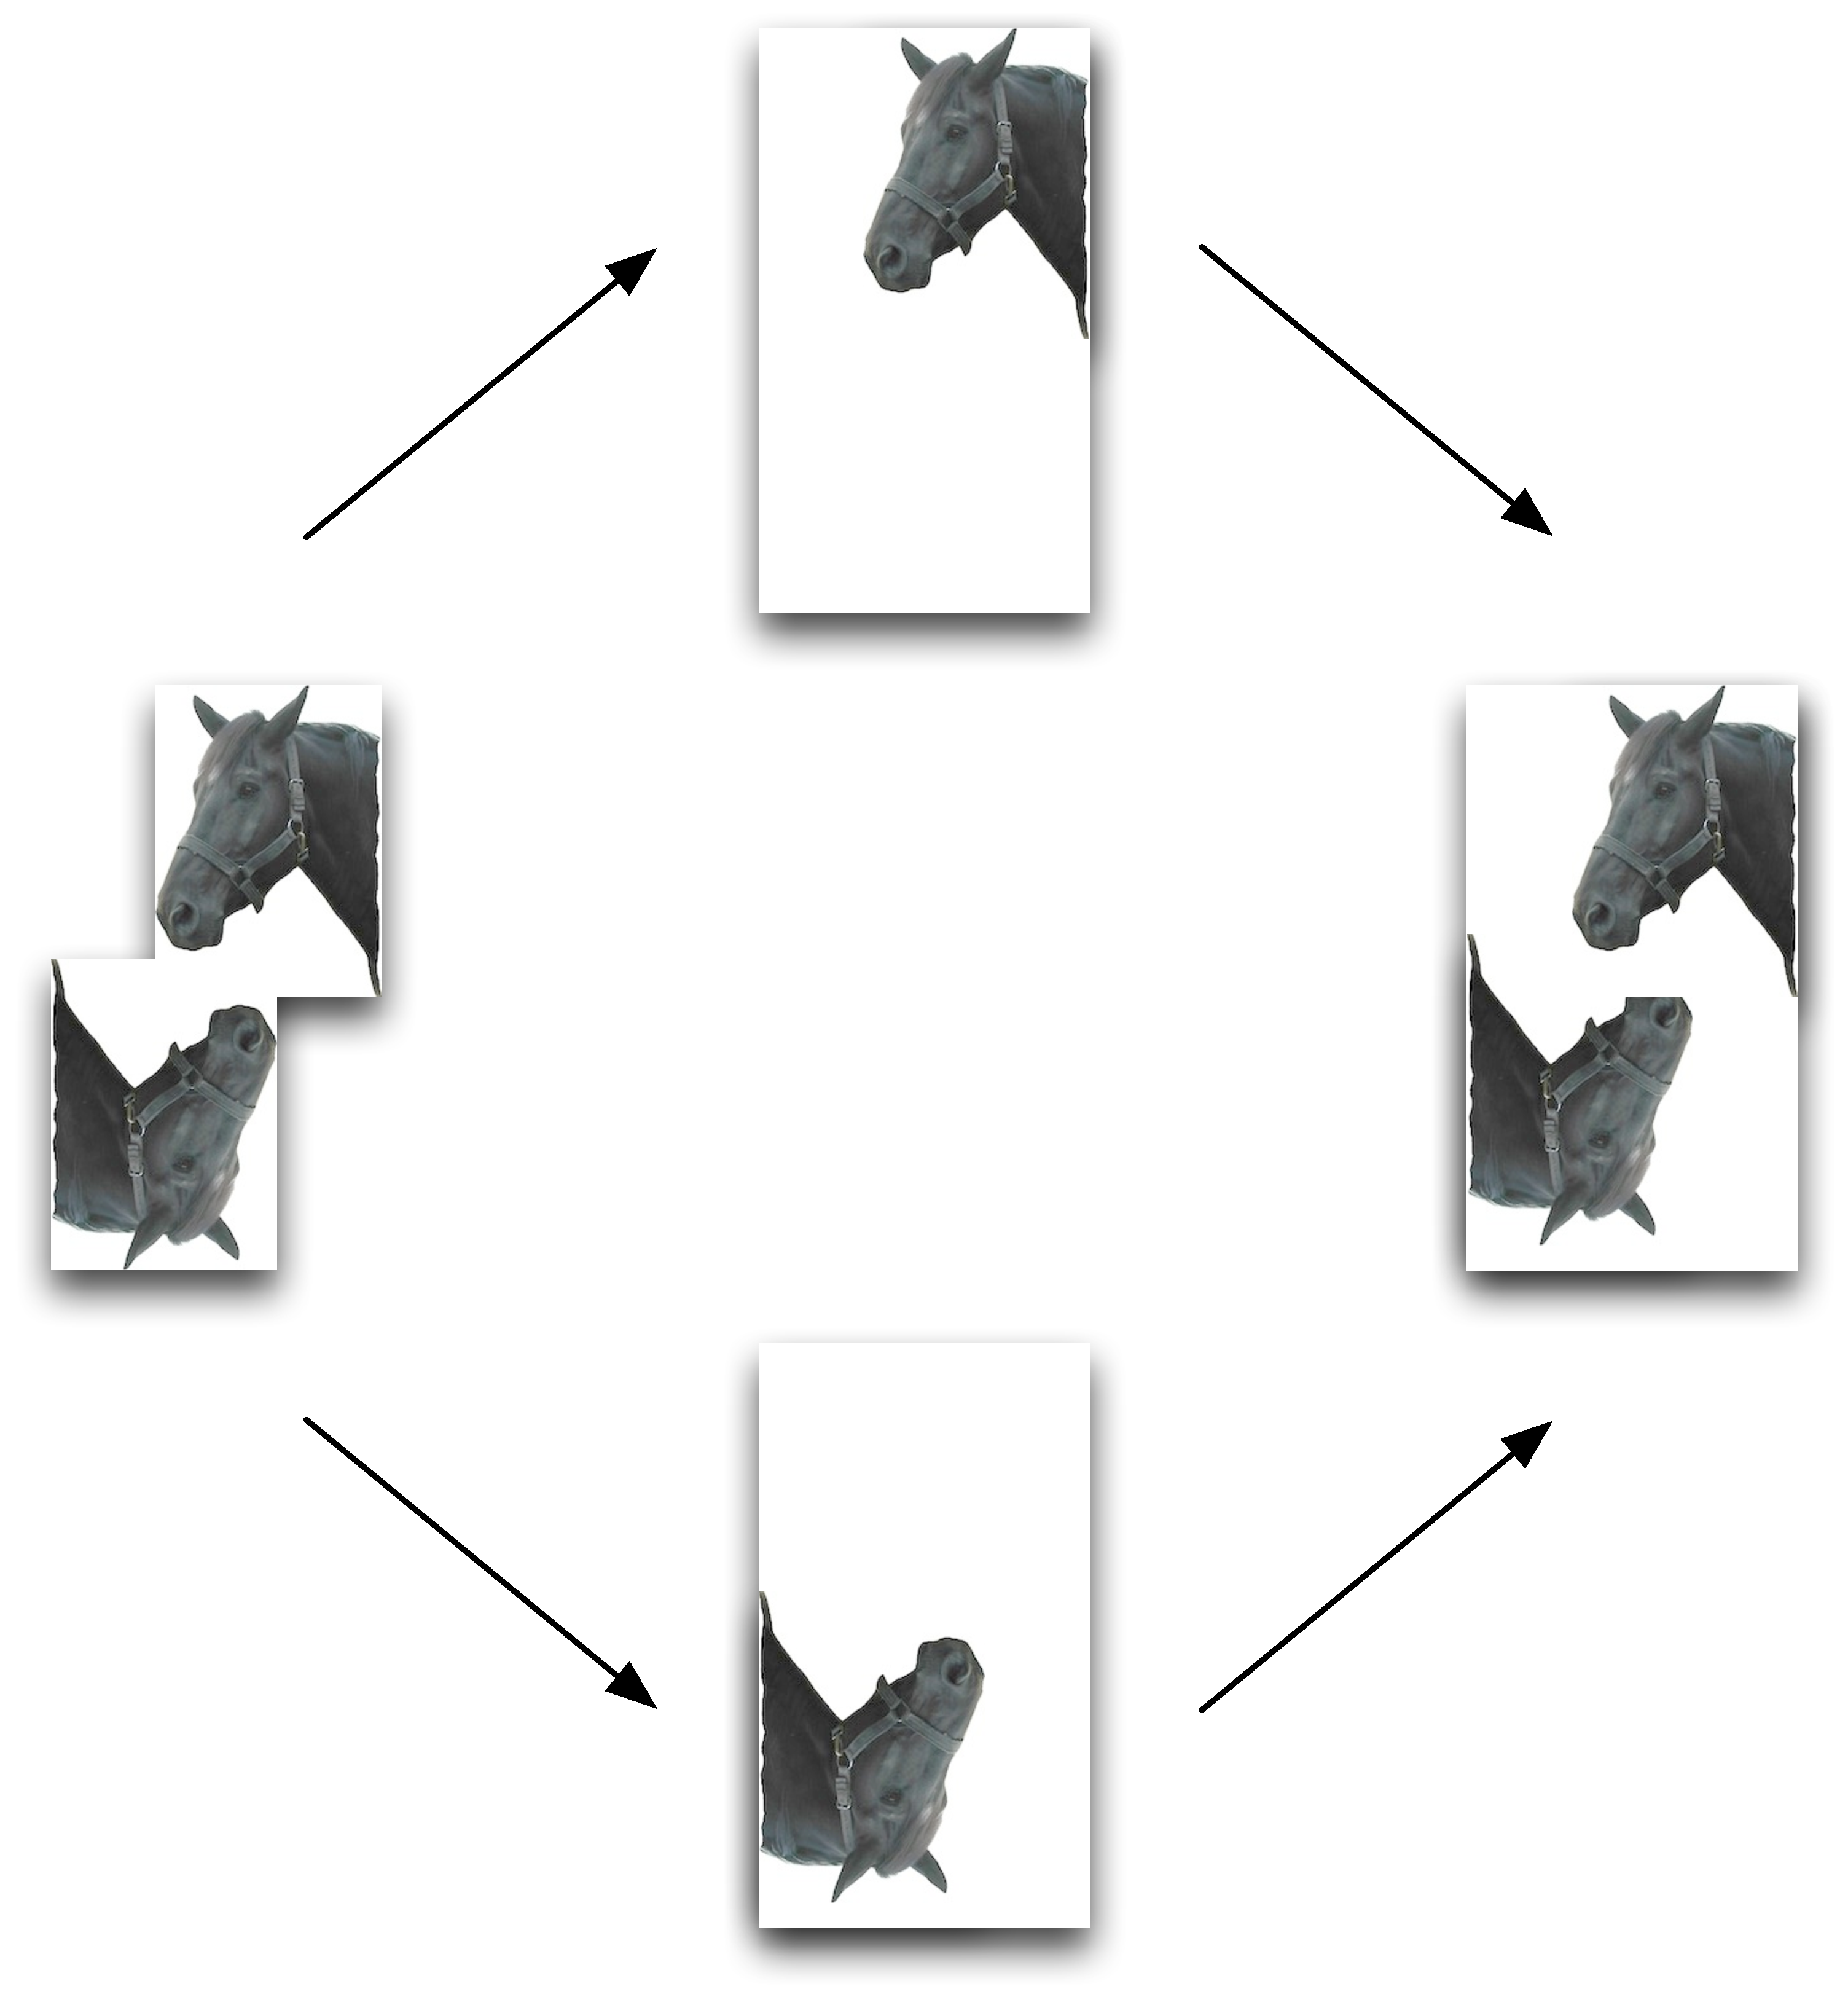
\includegraphics[width=3in]{Pictures/superPos.pdf}
\end{center}
\caption{Superimposing two \texttt{Images}.}
\label{superPos}
\end{figure}


\begin{exercises}


\item
Define functions to `pad out' a \texttt{Picture}
with an amount of white space, as shown in Figure \ref{superPos}.

You will need to think carefully about
the intended effect of the functions before you start to
implement them. You will need to have function parameters for the amount of padding
to the left, right, bottom and top of the image.

Note, in particular, that the \texttt{Position} of an
\texttt{Image} might change as a result of padding.

\item
Using the padding functions, define a superimposition function for
the \texttt{Image} type.

\item
How would you use \texttt{Image} superimposition to give analogues of 
\texttt{above} and \texttt{beside} for \texttt{Images}?

\item 
Define QuickCheck properties to check the implementation of the functions over the \texttt{Image} type. How many carry over from the \texttt{Picture} type, and how many have to be re-defined?

\index{pictures|)}
\index{extended exercise!positioned pictures|)}

\end{exercises}


\section{Extended exercise: supermarket billing}
\label{superBill}
\index{examples!supermarket billing|see{supermarket billing}}
\index{supermarket billing|(}

This collection of exercises looks at supermarket billing.\footnote{I am
grateful to Peter Lindsay {\em et\ al.\ }of the Department of
Computer Science at the University of New South Wales, Australia, for the
inspiration for this example, which was suggested by their lecture
notes.} The idea is to use the
list-manipulating techniques presented in Chapter \ref{tupleList}. In particular
we will be using list comprehensions and also the prelude functions
mentioned there. We will also expect local definitions -- as explained
in Section \ref{localDefs} -- to be used when
appropriate.

\begin{figure}[t]
\begin{alltt}
                          Haskell Stores\index{Haskell Stores@\verb+Haskell Stores+}
                     
                  Dry Sherry, 1lt...........5.40
                  Fish Fingers..............1.21
                  Orange Jelly..............0.56
                  Hula Hoops (Giant)........1.33
                  Unknown Item..............0.00
                  Dry Sherry, 1lt...........5.40
                       
                  Total....................13.90
\end{alltt}
\caption{A supermarket bill}
\label{basicBill}
\end{figure}


\subsection*{The problem}

A scanner at a supermarket checkout will produce from a basket
of shopping a list of bar codes,
like
\begin{alltt}
[1234,4719,3814,1112,1113,1234]
\end{alltt}
which has to be converted to a bill as shown in Figure \ref{basicBill}
We have to decide first how to model the objects involved. Bar codes and
prices (in pence) can be modelled by integers; names of goods by strings. We
say therefore that
\begin{alltt}
type Name    = String
type Price   = Int
type BarCode = Int
\end{alltt}
The conversion will be based on a \textbf{database}\index{database}
which links bar
codes, names and prices. As in the library, we use a list to model the
relationship. 
\begin{alltt}\minx{Database}
type Database = [ (BarCode,Name,Price) ]
\end{alltt}
The example database we use is
\begin{alltt}
codeIndex :: Database
codeIndex = [ (4719, "Fish Fingers" , 121),
              (5643, "Nappies" , 1010),
              (3814, "Orange Jelly", 56),
              (1111, "Hula Hoops", 21),
              (1112, "Hula Hoops (Giant)", 133),
              (1234, "Dry Sherry, 1lt", 540)]
\end{alltt}
The object of the script will be to convert a list of bar codes into a list
of \texttt{(Name,Price)} pairs; this then has to be converted into a string
for printing as above. We make the type definitions
\begin{alltt}
type TillType = [BarCode]
type BillType = [(Name,Price)]
\end{alltt} 
and then we can say that the functions we wish to define are 
\begin{alltt}
makeBill    :: TillType -> BillType\minx{makeBill}
\end{alltt}
which takes a list of bar codes to a list of name/price pairs,
\begin{alltt}
formatBill  :: BillType -> String\minx{formatBill}
\end{alltt}
which takes a list of name/price pairs into a formatted bill, and
\begin{alltt}
produceBill :: TillType -> String\minx{produceBill}
\end{alltt}
which will combine the effects of \texttt{makeBill} and
\texttt{formatBill}, thus
\begin{alltt}
produceBill = formatBill . makeBill
\end{alltt}
The length of a line in the bill is decided to be \texttt{30}. This is made a
constant, thus
\begin{alltt}
lineLength :: Int
lineLength = 30
\end{alltt}
Making \texttt{lineLength} a constant in this way means that to change the
\index{definition!constant!reason for}
length of a line in the bill, only one definition needs to be altered; if
\texttt{30} were used in each of the formatting functions, then each would have
to be modified on changing the line length. 
The rest of the script is developed through the sequences of
exercises which follow. 

\subsection*{Formatting the bill}
 
First we develop the \texttt{formatBill} function from
the bottom up: we design functions to format prices, lines, and the total, and
using these we finally build the \texttt{formatBill} function itself.

\begin{exercises}

\item
Given a number of pence, \texttt{1023} say, the pounds and pence parts are given
by \texttt{1023 `div` 100} and \texttt{1023 `mod` 100}. Using this fact, and the 
\texttt{show} function, define a function
\begin{alltt}
formatPence :: Price -> String
\end{alltt}
so that, for example, \texttt{formatPence 1023 = "10.23"}; you need to be
careful about cases like \texttt{"12.02"}.

\item
Using the \texttt{formatPence} function, define a function
\begin{alltt}
formatLine  :: (Name,Price) -> String
\end{alltt}
which formats a line of a bill, thus
\begin{alltt}
formatLine ("Dry Sherry, 1lt",540) 
               = "Dry Sherry, 1lt...........5.40\bs{n}"
\end{alltt}
Recall that \texttt{'\bs{n}'} is the newline character, 
that \texttt{++} can be used
to join two strings together, and that \texttt{length} will give the length of a
string. You might also find the \texttt{replicate} function useful.

\item
Using the \texttt{formatLine} function, define
\begin{alltt}
formatLines :: [ (Name,Price) ] -> String
\end{alltt}
which applies \texttt{formatLine} to each \texttt{(Name,Price)} pair, and joins the
results together. 

\item
Define a function 
\begin{alltt}
makeTotal :: BillType -> Price
\end{alltt}
which takes a list of \texttt{(Name,Price)} pairs, and gives the total of the
prices. For instance,
\begin{alltt}
makeTotal [(" ... ",540),(" ... ",121)] = 661
\end{alltt}

\item
Define the function
\begin{alltt}
formatTotal :: Price -> String
\end{alltt}
so that, for example,
\begin{alltt}
formatTotal 661 = "\bs{n}Total.....................6.61"
\end{alltt}

\item
Using the functions \texttt{formatLines}, \texttt{makeTotal} and \texttt{formatTotal},
define 
\begin{alltt}
formatBill :: BillType -> String\minx{formatBill}
\end{alltt} 
so that on the input
\begin{alltt}
[("Dry Sherry, 1lt",540),("Fish Fingers",121),
("Orange Jelly",56),("Hula Hoops (Giant)",133),
("Unknown Item",0),("Dry Sherry, 1lt",540)]
\end{alltt}
the example bill at the start of the section is produced.

\end{exercises}
\subsection*{Making the bill: bar codes into names and prices}

Now we have to look
at the database functions which accomplish the conversion of bar codes into 
names and prices.

\begin{exercises}

\item
Define a function
\begin{alltt}
look :: Database -> BarCode -> (Name,Price)
\end{alltt}
which returns the \texttt{(Name,Price)} pair corresponding to the \texttt{BarCode}
in the \texttt{Database}. If the \texttt{BarCode} does not appear in the database,
then the pair \texttt{("Unknown Item", 0)} should be the result.

Hint: using the ideas of the library database you might find that you
are returning a {\em list\/} of \texttt{(Name,Price)}
rather than a single value. You can assume
that each bar code occurs only once in the database, so you can extract
this value by taking the \texttt{head} of such a list {\em if it is non-empty}.

\item
Define a function
\begin{alltt}
lookup :: BarCode -> (Name,Price)
\end{alltt}
which uses \texttt{look} to look up an item in the particular database {\mi
codeIndex}. This function clashes with a function \texttt{lookup}
defined in the prelude; consult page \pageref{redefName} for details of how to
handle this.

\item
Define the function 
\begin{alltt}
makeBill   :: TillType -> BillType\minx{makeBill}
\end{alltt}
which applies \texttt{lookup} to every item in the input list. For instance,
when applied to \texttt{[1234,4719,3814,1112,1113,1234]} the result will be
the list of \texttt{(Name,Price)} pairs given in Exercise 6.25.
Note that \texttt{1113} does not appear in \texttt{codeIndex} and so is converted
to \texttt{("Unknown Item",0)}.

This completes the definition of \texttt{makeBill} and together
with 
\texttt{formatBill} gives the conversion program. 
\end{exercises}

\subsection*{Extending the problem}

We conclude with some further
exercises.

\begin{exercises}
\item
You are asked to add a discount for multiple buys
of sherry: for every two bottles bought, there is a %\pounds 
\texttt{1.00} discount. From the example list of bar codes
\begin{alltt}
[1234,4719,3814,1112,1113,1234]
\end{alltt}
the bill should be as illustrated in 
Figure \ref{newBill}.
\begin{figure}[t]
\begin{alltt}
                          Haskell Stores
                     
                  Dry Sherry, 1lt...........5.40
                  Fish Fingers..............1.21
                  Orange Jelly..............0.56
                  Hula Hoops (Giant)........1.33
                  Unknown Item..............0.00
                  Dry Sherry, 1lt...........5.40
                     
                  Discount..................1.00
                     
                  Total....................12.90
\end{alltt}
\caption{Bills with `multibuy' discounts.}
\label{newBill}
\end{figure}
You will probably find it helpful to define functions
\begin{alltt}
makeDiscount :: BillType -> Price
formatDiscount :: Price -> String
\end{alltt}
which you can use in a redefined
\begin{alltt}
formatBill :: BillType -> String
\end{alltt}

\item
Design functions which update the database of bar codes. You will need a
function to add a \texttt{BarCode} and a \texttt{(Name,Price)} pair to the {\mi
Database}, while at the same time removing any other reference to the bar
code already present in the database.

\item
Re-design your system so that bar codes which do not appear in the database
give no entry in the final bill. There are (at least) two ways of doing this.
\begin{titemize}
\item Keep the function \texttt{makeBill} as it is, and modify the 
formatting functions, or
\item modify the \texttt{makeBill} function to remove the `unknown item' pairs.
\end{titemize}


\item
{[Harder]}
How appropriate would it be to test your supermarket billing system using QuickCheck? Could you check parts of the system using QuickCheck? Could you use it to test the whole system, or could you do both?


\item
{[Project]} Design a script of functions to analyse collections
of sales. Given a list of \texttt{TillType}, produce a table
showing the total sales of each item. You might also analyse
the bills to see which {\em pairs\/} of items are bought
together; this could assist with placing items in the
supermarket.


\index{supermarket billing|)}
\end{exercises}

\section{Extended exercise: cards and card games}
\label{cardGames}
\index{extended exercise!card games|(}

\begin{wrapfigure}[8]{r}{5cm}
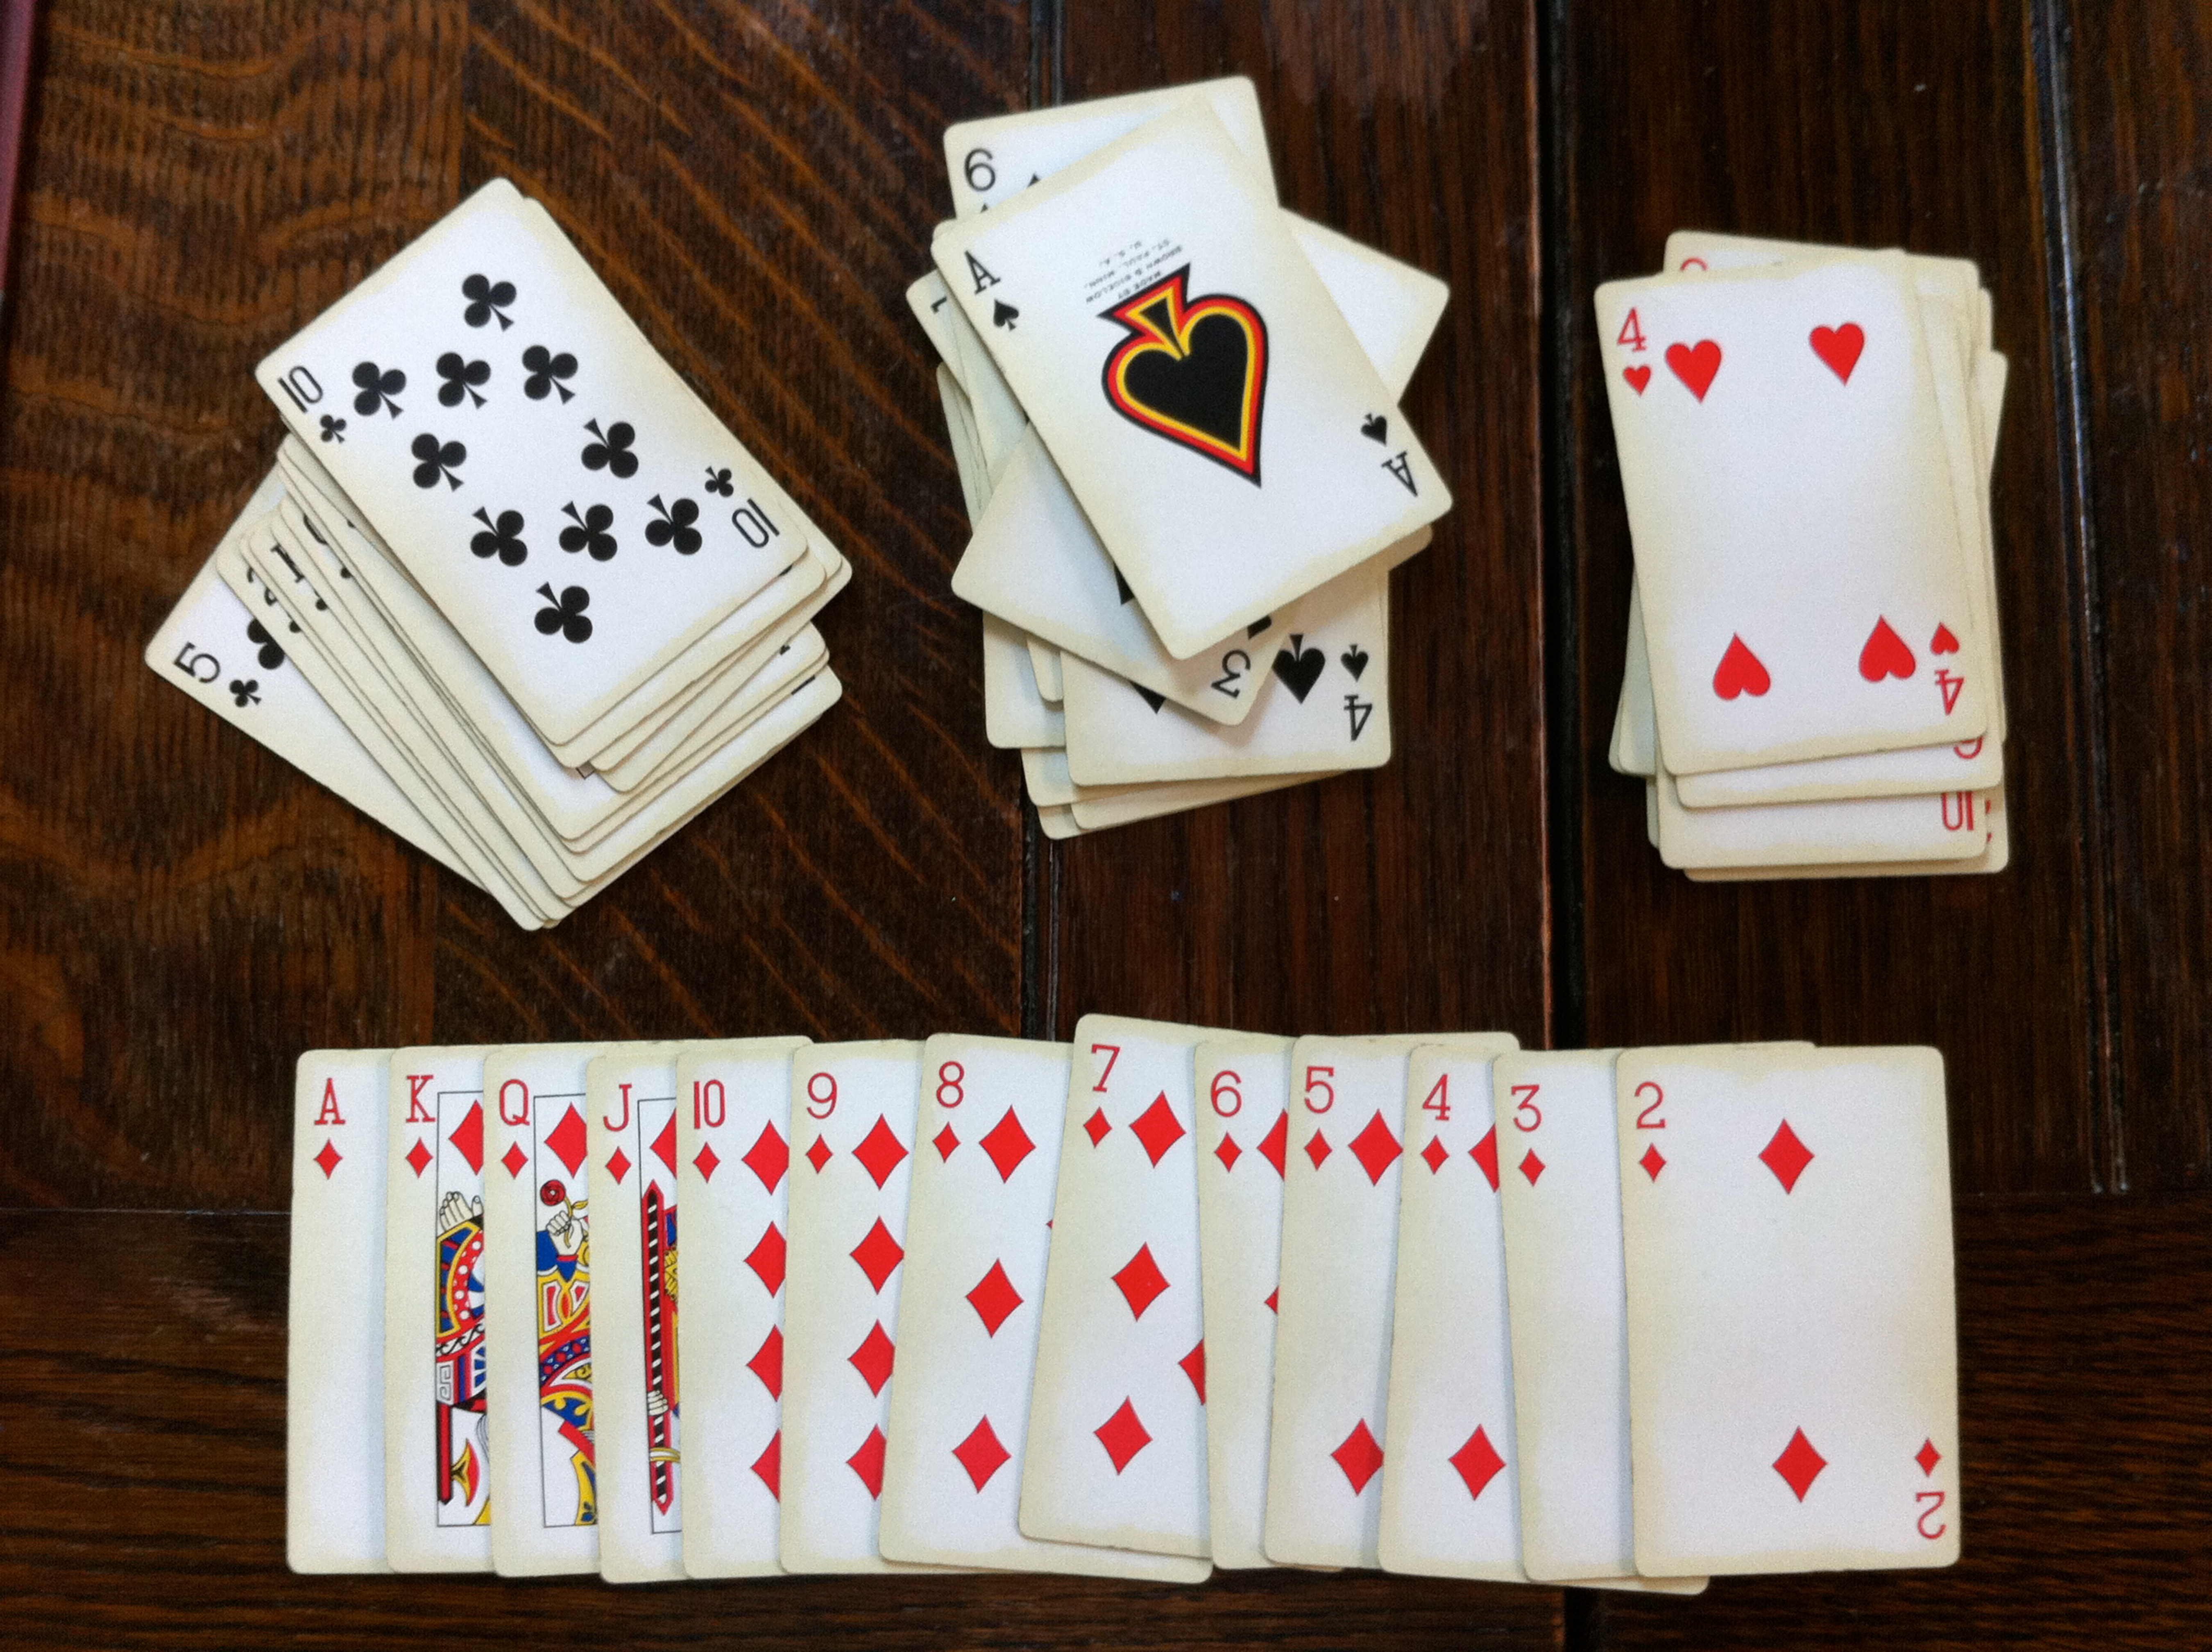
\includegraphics[width=5cm]{Pictures/Cards.pdf}
\end{wrapfigure}
An British deck (or pack) of cards has four suits: spades (\spade), hearts (\heart), diamonds (\dia) and clubs (\club). 

Each suit\index{suit} contains cards 2 to 10, and the court cards, Jack, Queen, King and Ace. The values of the cards increase in the same order, so, for example, a 9 beats a 2, a King beats a 10, and an Ace beats everything (in this discussion we're taking ``Aces high'').

\begin{exercises}

\item
Define a type \texttt{Suit} to represent \emph{suits} and a type \texttt{Value} to represent the \emph{value} of cards. Using these or otherwise, define a type \texttt{Deck} to represent a deck of cards. You may use type synonyms (\texttt{type}) or data type definitions (\texttt{data}), or both. 

\item Try to give a rationale for the choices you have made in answering the previous question: if you can, give alternative definitions which use the other mechanism, and compare your solutions. 

\end{exercises}

\begin{wrapfigure}[7]{r}{2cm}
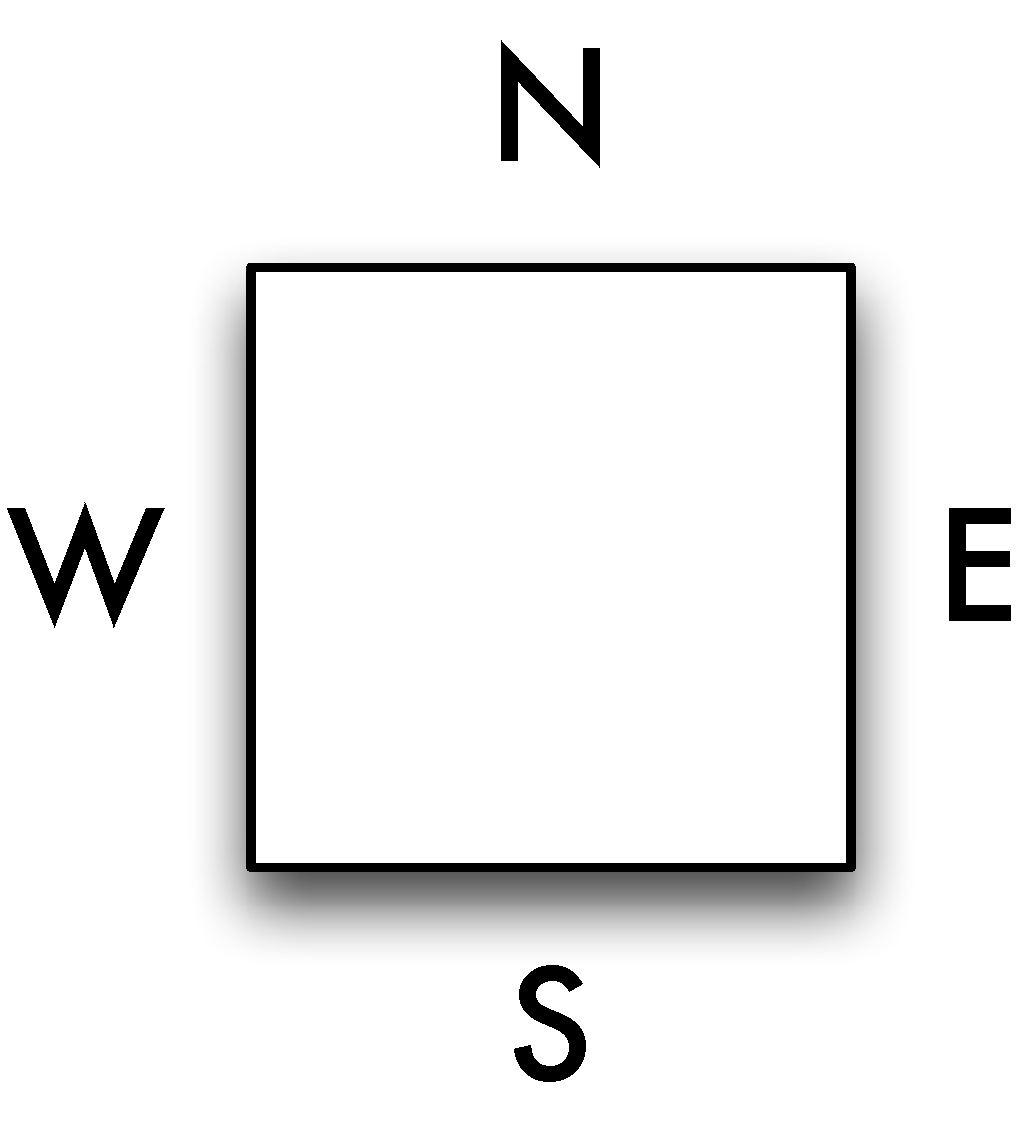
\includegraphics[width=2cm]{Pictures/NESW.pdf}
\end{wrapfigure}
\noindent
Many card games involve the idea of each player playing one card in turn, called a \emph{trick}.\index{trick} Traditionally for games like whist and bridge the players are called after the points of the compass: North, South, East and West. The play is in clockwise order: if East is the player to start (to \emph{lead}) then the players South, West and North follow in that order.

\begin{exercise}

\item
Define a type \texttt{Player} to represent the four players.

\end{exercise}

\noindent
There is an important rule about how players should choose cards to play.
A player should \emph{follow suit}: that is, if they can, they must play a card from the same suit as the card that was led (the card played by the person starting). A player can only play from a different suit if she has no cards left in the suit that was led.

\begin{wrapfigure}[12]{r}{3cm}
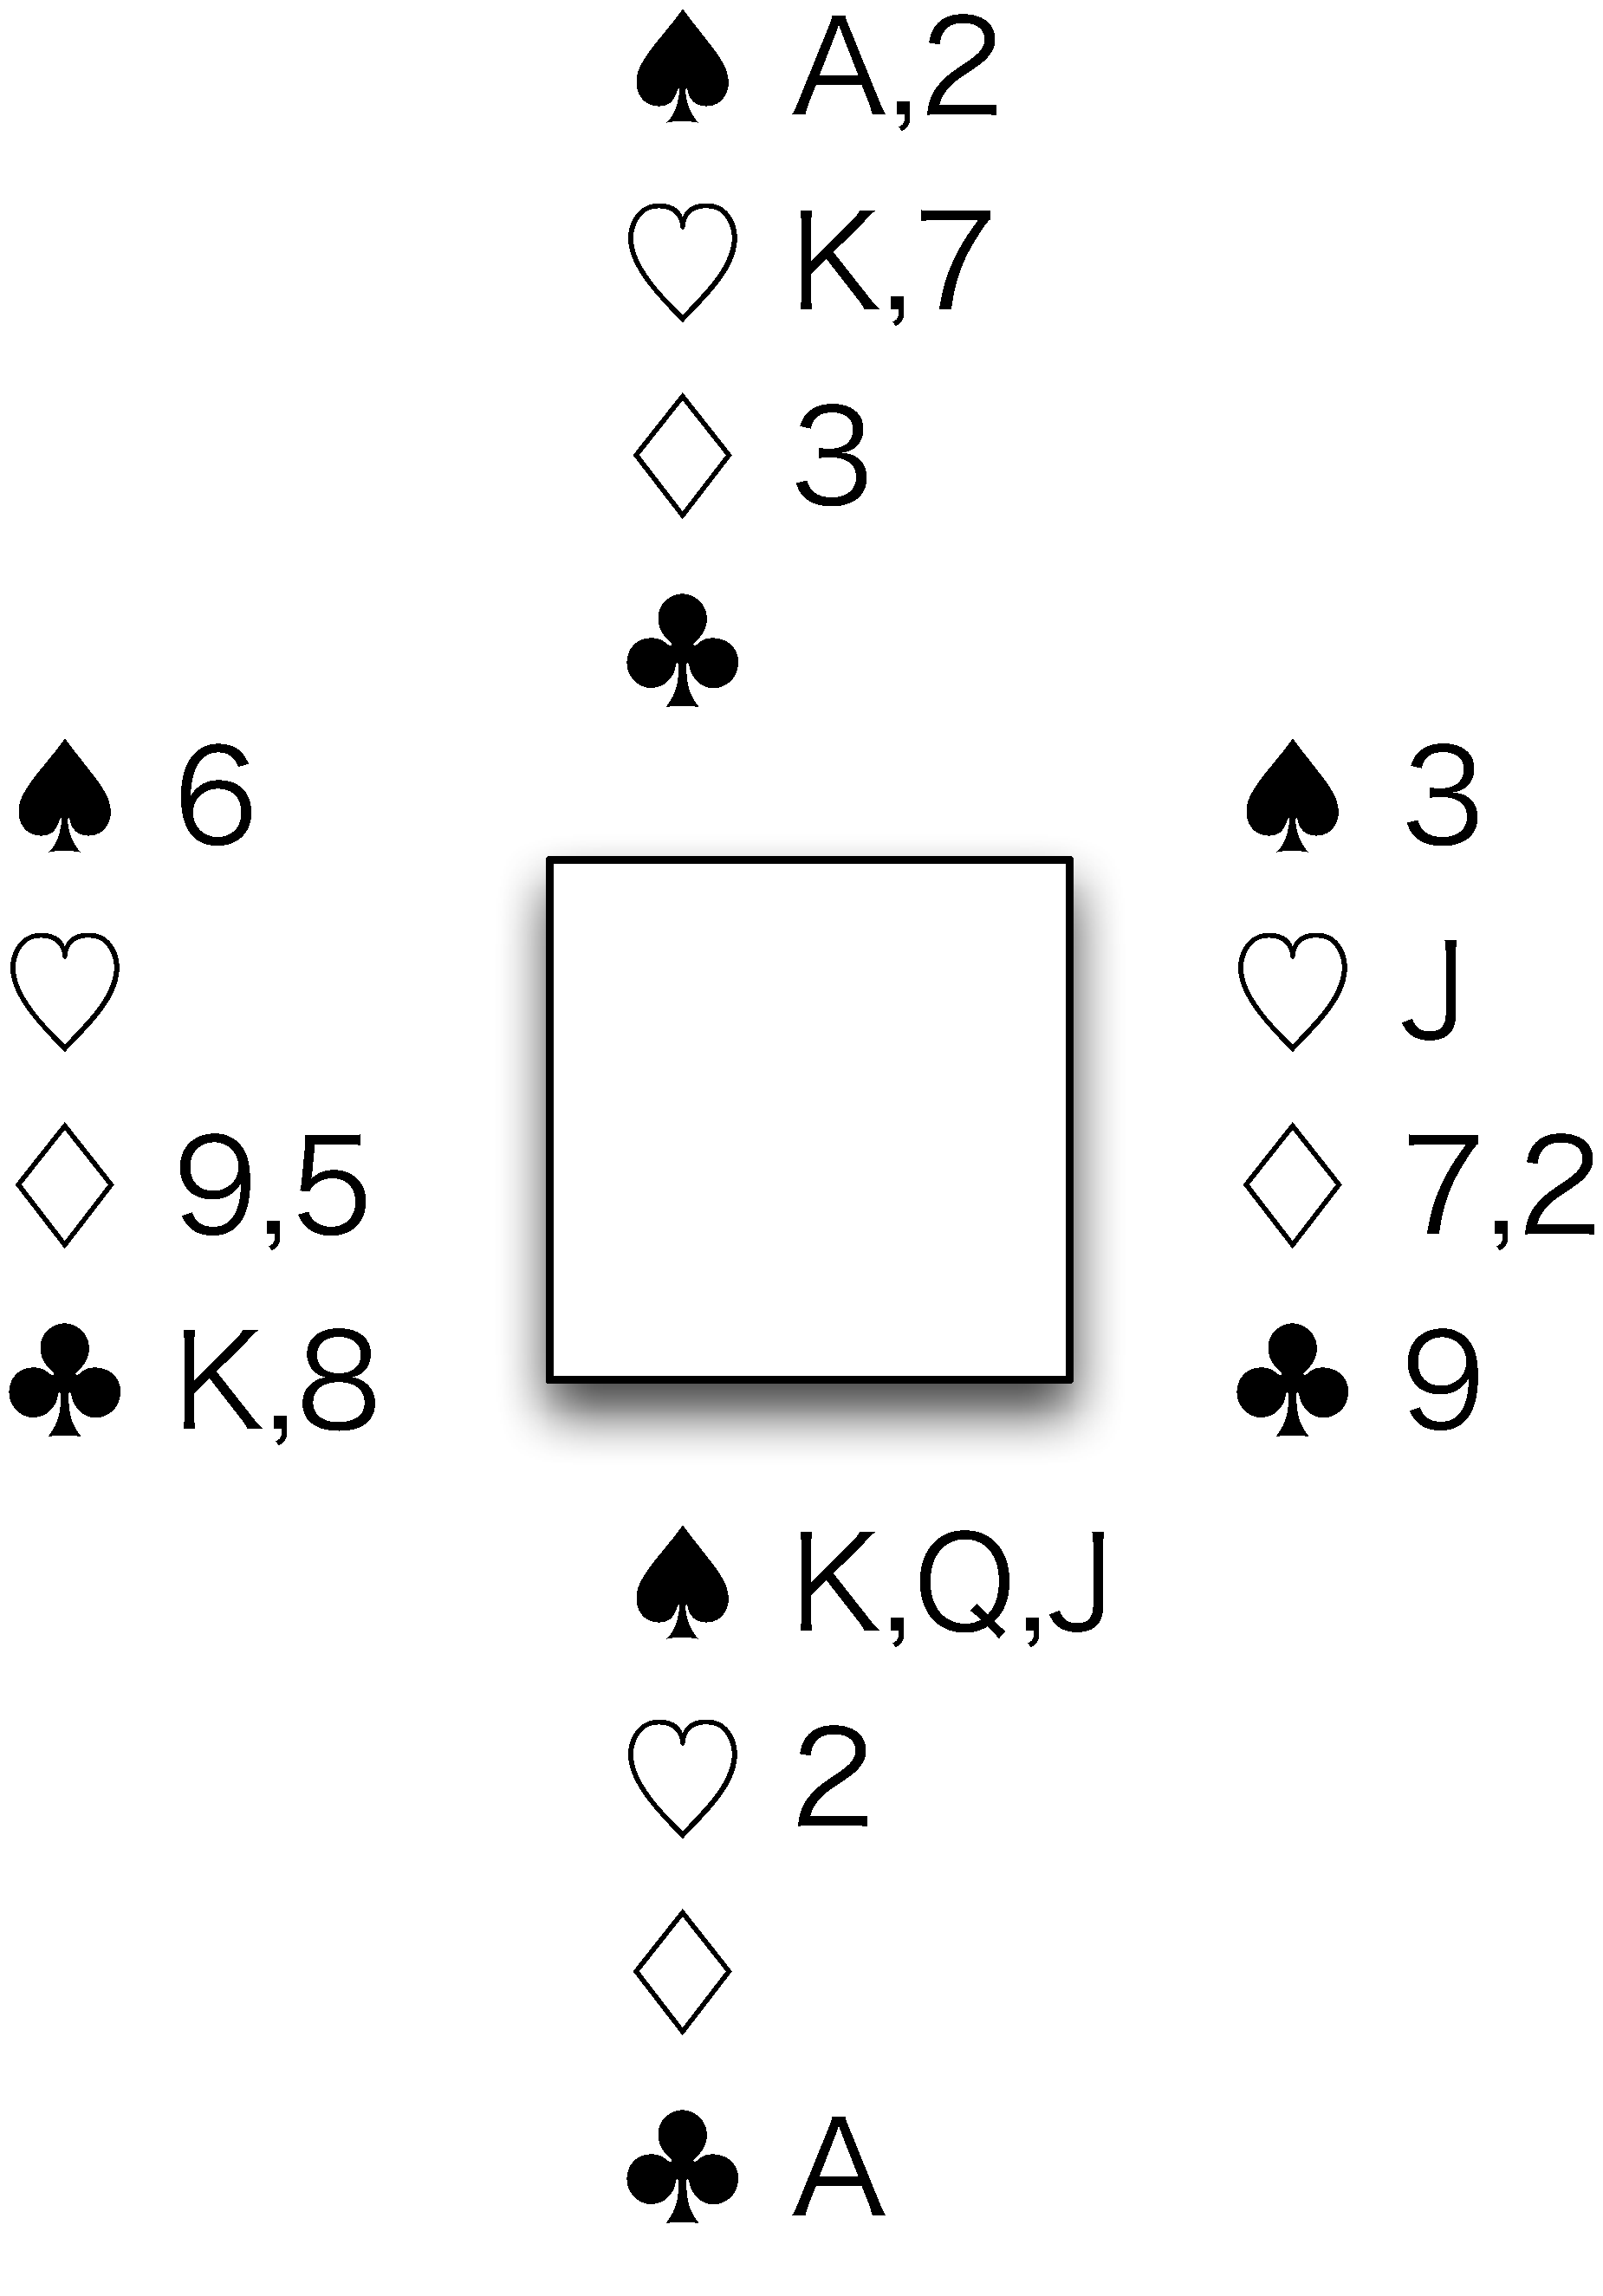
\includegraphics[width=3cm]{Pictures/Hand1.pdf}
\end{wrapfigure}
Let's have a look at an example. Suppose that each of the players has five cards left, as shown to the right. Suppose also that East is to lead and that she plays the Jack of Hearts.  
South has no choice: he has to play the 2 of Hearts. West has no Hearts, so she can choose any other card to play. Finally, North has a choice of two Hearts: the King or the 7, let's suppose that he plays the King.

Who wins the trick? Let's suppose first that there is no trump suit. The highest Heart will win the trick, and that's the King. Why Hearts? Because a Heart was led by East.\\
\hspace*{0.5cm} If there is a \emph{trump}\index{trump} suit, then the highest trump card wins if any trumps have been played, but remember that you can only play a trump if you're unable to follow suit. If Spades were trumps in this case, then West could win the trick by playing the 6 of Spades, no one else can play a trump as they are able to follow suit.

\begin{exercises}

\item
How would you represent a trick? Define a type \texttt{Trick}, using either a \texttt{type} or a \texttt{data} definition. Remember that you need to know which player has played which card, and also who led.

\item
Define a function
\begin{alltt}
winNT :: Trick -> Player
\end{alltt}
which decides the winner of a trick, assuming that there is no trump suit.

\item
Define a function
\begin{alltt}
winT :: Suit -> Trick -> Player
\end{alltt}
which decides the winner of a trick, assuming that there is a trump suit, which is passed in as the first argument.

\item
Define a type \texttt{Hand} which represents the collection of cards held by a player at one point during a game. In the earlier example, the hand held by North is \spade A, 2; \heart K, 7; \dia 3 (and no \club{} cards). 

\item Define a type \texttt{Hands} which describes the hands held by the four players at one point in the game. This should represent the four hands shown in the diagram above, for example.

\item
Define a function
\begin{alltt}
checkPlay :: Hands -> Trick -> Bool
\end{alltt}
which checks whether the play in a particular trick is both \emph{possible} and \emph{legal}. It should be possible in the sense that the card played by each player (given in the \texttt{Trick}) should be in their hand, as given in the \texttt{Hands}. It should be legal in following the rule that players should \emph{follow suit} if they can.
\end{exercises}

\noindent
What does a game look like? As there are 52 cards, when dealt to four players this results in each player receiving 13 cards. There will therefore be thirteen tricks played. In whist and bridge pairs of players -- North/South and East/West -- play together, so in an game of 13 tricks one side or the other will win.

\begin{exercises}

\item
Define a type \texttt{Team} to represent the two teams North/South and East/West. Define a function 
\begin{alltt}
winnerNT :: [Trick] -> Team
\end{alltt} 
which will give the winning team from the list of tricks, assuming that there are no trumps. Also define the function
\begin{alltt}
winnerT :: Suit -> [Trick] -> Team
\end{alltt} 
where the trump suit is passed in as the first argument.

\item {[Harder]}
Define a function 
\begin{alltt}
checkPlay :: [Trick] -> Bool
\end{alltt}
which checks whether the play in each trick is both \emph{possible} and \emph{legal}.
\emph{Hint:} you will need to deduce the hand in each case from the cards played subsequently: once you have done this, you can use \texttt{checkPlay} as defined earlier.

\end{exercises}
\index{extended exercise!card games|)}

 
\begin{summary}

This chapter has shown how the combination of list comprehensions and the built-in
functions from the prelude give us a powerful repertoire of tools with
which to build definitions over particular list types. This was evident
in the \texttt{Picture} example as well as in the case studies, and
these also gave an opportunity to see the way in which a larger program
was built as a collection of related functions.
returning a member of the same list type. The example in Section \ref{cardGames} particularly emphasised the process of choosing types to represent the various entities in the domain in question.

Section \ref{HaskellLibs} contains vital information about the libraries available in Haskell, including how to download them, how to find out more about their contents and how to search for functions performing particular tasks. 

In the next chapter we'll find out about how to define functions over lists for ourselves.
\end{summary}

%\end{document}

%\documentclass{book}\usepackage{sjtfonts}\usepackage{includegraphics}\usepackage{alltt}\usepackage{latexsym}
%\usepackage{array}
%\begin{document}\input{defs0}%		miradefs.tex 		    June 1994

% opening and closing a quoted Miranda section

\newcommand{\mira}{\noindent\hrulefill\nopagebreak\so}
\newcommand{\arim}{\nopagebreak\st\hrulefill\\}

% backslash in the Miranda environment
% Only feasible approach is to use \verb+\+
% in line!

%\newcommand{\bs}{$\mi\backslash\!\!$}
%\newcommand{\lbs}{\mbox{\verb+\+}}

% ignoring part of the input

\newcommand{\ignore}[1]{}

% a blank line in a Miranda section

\newcommand{\bl}{\mbox{\ }}

% Signalling a diffculty.

\definecolor{light-gray}{gray}{0.95}

\newcommand{\beware}[2]
 {\medskip\noindent\colorbox{light-gray}{\parbox{\textwidth}
 {\mbox{\large\textbf{#1}} \medskip\noindent\\ #2}\medskip\noindent}}

% Subscripting in Miranda text
\newcommand{\subscr}[2]{\mbox{${\mbox{\texttt{#1}}}_{\mbox{\texttt{#2}}}$}}

%\newcommand{\subscr}[2]{\mbox{${\mbox{\mi #1}}_{\mbox{\smtt #2}}$}}
\newcommand{\aone}{\subscr{a}{1}}
\newcommand{\atwo}{\subscr{a}{2}}
\newcommand{\ak}{\subscr{a}{k}}

\newcommand{\aoneone}{\subscr{a}{1,1}}

\newcommand{\eone}{\subscr{e}{1}}
\newcommand{\etwo}{\subscr{e}{2}}
\newcommand{\ei}{\subscr{e}{i}}
\newcommand{\er}{\subscr{e}{r}}

\newcommand{\fone}{\subscr{f}{1}}
\newcommand{\fl}{\subscr{f}{l}}

\newcommand{\gone}{\subscr{g}{1}}
\newcommand{\gtwo}{\subscr{g}{2}}
\newcommand{\gi}{\subscr{g}{i}}
\newcommand{\gr}{\subscr{g}{r}}

\newcommand{\hone}{\subscr{h}{1}}
\newcommand{\hl}{\subscr{h}{l}}

\newcommand{\pone}{\subscr{p}{1}}
\newcommand{\ptwo}{\subscr{p}{2}}
\newcommand{\pk}{\subscr{p}{k}}

\newcommand{\qone}{\subscr{q}{1}}
\newcommand{\qtwo}{\subscr{q}{2}}
\newcommand{\qk}{\subscr{q}{k}}

\newcommand{\rone}{\subscr{r}{1}}
\newcommand{\rtwo}{\subscr{r}{2}}

\newcommand{\tone}{\subscr{t}{1}}
\newcommand{\ttwo}{\subscr{t}{2}}
\newcommand{\tn}{\subscr{t}{n}}

\newcommand{\vone}{\subscr{v}{1}}
\newcommand{\vtwo}{\subscr{v}{2}}
\newcommand{\vn}{\subscr{v}{n}}

% for regular expressions

\newcommand{\stone}{\subscr{st}{1}}
\newcommand{\sttwo}{\subscr{st}{2}}
\newcommand{\stn}{\subscr{st}{n}}
\newcommand{\rthree}{\subscr{r}{3}}

\newcommand{\eps}{$\varepsilon$}
\newcommand{\trans}[1]{\stackrel{\mbox{\tt #1}}{\longrightarrow}}



% superscript in Miranda text

\newcommand{\superscr}[2]{\mbox{${\mbox{\mi #1}}^{\mbox{\smtt #2}}$}}

% Not equals in Miranda text

\newcommand{\noteq}{\makebox[0pt][l]{=}/}
\newcommand{\overslash}{\makebox[0pt][l]{/}}

% Definitions in complexity chapter

\newfont{\oldSym}{cmsy10}
\newcommand{\Th}{\boldmath$\oldSym\Theta$}
\newcommand{\pow}[1]{\^{}#1}
\newcommand{\leqq}{$\leq$}
\newcommand{\geqq}{$\geq$}
\newcommand{\lll}{$\ll$}
\newcommand{\eqq}{$\equiv$}
\newcommand{\ltwo}{\subscr{log}{2}}

% Indexing

\newcommand{\minx}[1]{\index{#1@{\ttfamily{}#1}}}


\chapter{Defining\,functions over lists}
\chapstart
\label{defFunLists}
\index{lists!defining functions|(}
\index{design!list functions|(}

We have already seen how to define a variety of functions over lists using a 
combination of list comprehensions and the built-in list processing functions
in the Haskell prelude and libraries. This chapter looks `under the bonnet' and explains how 
functions over lists can be defined by means of
recursion. This will allow us  to define the prelude functions we
have already been using, as well as letting us look at a wider class of
applications, including sorting and a case study of text processing.

The chapter begins with a summary of the mechanism of pattern matching,
and continues with a justification and explanation of recursion echoing
the discussion in Chapter \ref{writingProgs}. We then explore a variety
of examples both of functions defined by primitive recursion and of more
general recursive functions, and conclude with the case study mentioned
earlier.

\section{Pattern matching revisited}
\label{pattMatchRevisit}
\index{pattern matching|(}

We have seen that function definitions take the form of conditional equations like
\begin{alltt}
mystery :: Integer -> Integer -> Integer
mystery x y 
  | x==0        = y
  | otherwise   = x
\end{alltt}
where a choice of two alternatives is made by guards; we can rewrite
this into two equations, thus
\begin{alltt}
mystery 0 y = y\hfill(mystery.1)
mystery x y = x\hfill(mystery.2)
\end{alltt}
where we distinguish between the two cases by using a pattern -- here
the literal \texttt{0} -- instead of a variable. Just as for guards,
the equations are applied \textbf{sequentially}\index{pattern matching!sequentiality}, 
and so \texttt{(mystery.2)} will only be used
in cases that \texttt{(mystery.1)} does not apply.

Another aspect of this definition is that \texttt{y} is not used on the
right-hand side of \texttt{(mystery.2)}. Because of this we do not need to give a name
to the second argument in this case, and so we can replace the variable
y with the \textbf{wildcard} `\verb+_+' which matches anything, thus\index{wildcard (`\symbol{95}')}\index{pattern matching!wildcard (`\symbol{95}')}
\begin{alltt}\minx{\symbol{95}}
mystery 0 y = y
mystery x _ = x
\end{alltt}
We have therefore seen that pattern matching can be used for
distinguishing between certain sorts of 
\textbf{cases} in function definitions. We have also seen pattern matching used
to \textbf{name the components} of tuples, as in
\begin{alltt}
joinStrings :: (String,String) -> String
joinStrings (st1,st2) = st1 ++ "\bs{t}" ++ st2
\end{alltt}
where the variables \texttt{st1} and \texttt{st2} will be matched with
the components of any argument.


We can see the case switching and extracting components in action together in the definition of the function to give the \texttt{area} of a \texttt{Shape}, first seen in Section \ref{areaDef}:
\begin{alltt}\minx{Shape}\minx{area}
area :: Shape -> Float
area (Circle r)      = pi*r*r
area (Rectangle h w) = h*w
\end{alltt}
The two equations apply to different kinds of shape, and within each equation the appropriate information is extracted: from a circle its radius, \texttt{r}, and from a rectangle its height, \texttt{h}, and width, \texttt{w}. We see exactly this combination of case switching and component extraction in working with lists too, as we see in
the next section.

\subsection*{Summarizing patterns}

A pattern can be one of a number of things:
{\raggedright
\begin{itemize}
\item A {\bf literal value} such as \texttt{24}, \texttt{'f'} or
\texttt{True}; an argument matches this pattern if it is equal to the
value.\index{pattern matching!literals}
\item A {\bf variable} such as \texttt{x} or
\texttt{longVariableName}; any argument value will match
this.\index{pattern matching!variables}
\item A {\bf wildcard} `\verb+_+'; any argument
value will match this.
\item A {\bf tuple pattern}
\texttt{(\pone,\ptwo,...,\subscr{p}{n})}. To match this, an
argument must be of the form \texttt{(\vone,\vtwo,...,\vn)},
and each \texttt{\subscr{v}{k}} must match
\texttt{\subscr{p}{k}}.
\item A {\bf constructor} applied to a number of patterns \texttt{(C \pone\ \ptwo,...,\subscr{p}{n})}. To match this the argument must be an application of the constructor \texttt{C} to n arguments: each of the each \texttt{\subscr{v}{k}} must match the corresponding pattern \texttt{\subscr{p}{k}}. We'll look at this case again in the next section.\index{pattern matching!constructors}
\end{itemize}
} % end \raggedright

\noindent
In a function definition we have a number of conditional
equations, each of which will have a left-hand side in which the
function is applied to a number of patterns. When the function is
applied we try to match the arguments with the patterns in
sequence, and we use the first equation which applies; pattern
matching in Haskell is thus \textbf{sequential}, in a similar way to
the conditions expressed by guards.
\index{pattern matching!sequentiality of}

\section{Lists and list patterns}

Every list is either \textbf{empty}, \texttt{[]},\minx{[]} or is non-empty.
In the latter case -- take the example \texttt{[4,2,3]}\minx{:}
-- then it can be written in the form \texttt{x:xs}, where \texttt{x}
is the first item in the list and \texttt{xs} is the remainder of the list; in our example, we have
\texttt{4:[2,3]}. We call \texttt{4} the \textbf{head}\index{lists!head} of the
list and \texttt{[2,3]} the \textbf{tail}.\index{lists!tail}

What is more, every list can be built up from the
empty list by repeatedly applying `\texttt{:}', and indeed Haskell lists
are represented in that way internally. Our example list can be thought
of as being built step-by-step from the right, like this
\begin{alltt}
[]      3:[] = [3]      2:[3] = [2,3]      4:[2,3] = [4,2,3]
\end{alltt}
and we can write the list using `\texttt{:}' repeatedly like this:
\begin{alltt}
4:2:3:[]
\end{alltt}
Note that here we use the fact that `\texttt{:}' is \textbf{right associative}, 
so that for any values of \texttt{x}, \texttt{y} and
\texttt{zs},
\begin{alltt}
x:y:zs = x:(y:zs)
\end{alltt}
It is also not hard to see that \texttt{4:2:3:[]} is the 
{\em only\/} way that \texttt{[4,2,3]}
can be built using `\texttt{:}'.
The operator `\texttt{:}', of type
\begin{alltt}
a -> [a] -> [a]
\end{alltt}
therefore has a special role to play for lists: it is a
\textbf{constructor}\index{constructor}\index{lists!constructor} for
lists, since every list can be built up in a unique way from [] and
`\texttt{:}'. For historical reasons we sometimes call this constructor
\textbf{cons}\index{cons}. Not all functions that build lists are constructors:
\texttt{++} can be used to build lists, but this construction will not
be unique, since, for example
\begin{alltt}
[1] ++ [2,3] = [1,2,3] = [1,2] ++ [3]
\end{alltt}

\subsection*{Pattern-matching definitions}

If we want to make a definition covering all cases of lists we can write
\begin{alltt}
fun xs = ....
\end{alltt}
but more often than not we will want to distinguish between empty and
non-empty cases, as in the prelude functions
\begin{alltt}
head             :: [a] -> a
head (x:_)        = x

tail             :: [a] -> [a]
tail (_:xs)       = xs

null             :: [a] -> Bool
null []           = True
null (_:_)        = False
\end{alltt}
where \texttt{head} takes the first item in a non-empty list,
\texttt{tail} takes all but the head of a non-empty list and
\texttt{null} checks whether or not a list is empty. 

In the definition
of \texttt{null} the pattern \verb+(_:_)+ will match any non-empty list,
but it gives no names for the head and tail; when we need to name one of
these, as in \texttt{tail}, then a different pattern,
\verb+(_:xs)+,
is used.

It has become an informal convention in the Haskell community to write
variables over lists in the form \texttt{xs}, \texttt{ys}  (pronounced `exes', `whyes')
and so on,\minx{xs}\minx{ys}
with variables \texttt{x}, \texttt{y}, \ldots ranging over their
elements. We will -- when using short variable names -- often use that convention.\index{conventions!list variables}

We can now go back to the final case of \textbf{pattern matching}. A \textbf{constructor
pattern} over lists will either be \texttt{[]} or will have the form \texttt{(p:ps)}
where \texttt{p} \index{pattern matching!constructors}
and \texttt{ps} are themselves patterns. \index{constructor!pattern matching}
\begin{itemize}
\item
A list matches \texttt{[]} exactly when it is empty.
\item
A list will match the pattern \texttt{(p:ps)}
if it is non-empty, and also if its head matches the pattern
\texttt{p} and its tail the pattern \texttt{ps}. 
\end{itemize}
In the case of the
pattern \texttt{(x:xs)}, it is sufficient for the argument to be 
non-empty to match the pattern; the head of the argument is matched with \texttt{x} and
its tail with \texttt{xs}. 
Let's look at some examples in more detail.
\begin{itemize}
\item
The list \texttt{[2,3,4]} will match \texttt{(p:ps)}, because \texttt{2} is matched with \texttt{p} and \texttt{[3,4]} with \texttt{ps}.
\item
The list \texttt{[2,3,4]} will match \texttt{(q:(p:ps))}, because \texttt{2} is matched with \texttt{q}, \texttt{3} is matched with \texttt{p} and \texttt{[4]} with \texttt{ps}.
\item
The list \texttt{[5]} will \textbf{not} match \texttt{(q:(p:ps))}; this is because \texttt{5} can match with \texttt{q}, but \texttt{[]} cannot be matched with \texttt{(p:ps)}.
\end{itemize}

\begin{figure}[t]
\beware{Patterns and Parentheses}{\index{pattern matching!and parentheses}\index{parentheses}
A pattern involving a constructor like `\texttt{:}' will always have to be
parenthesized, since function application binds more tightly than any
other operation. This means that writing 
\begin{alltt}
f x:xs
\end{alltt} 
will be interpreted as 
\begin{alltt}
(f x):xs
\end{alltt} 
 and not as \begin{alltt}
f (x:xs)\end{alltt} 
as we would like.}
\end{figure}

\subsection*{The \texttt{case} construction}
\index{pattern matching!in expressions}
\minx{case}


So far we have seen how to perform a pattern match over the arguments of
functions; sometimes we might want to pattern match over other values. This
can be done by a \texttt{case} expression, which we introduce by means of an
example.

Suppose we are asked to find the first digit in the string \texttt{st},
returning 
\texttt{'\bs{0}'} in case no digit is found. We can use the function \texttt{digits} of
Section \ref{listComps}
to give us the list of all the digits in the string:
\texttt{digits st}. If this is not empty, that is if it matches \texttt{(x:\_)},
we want to return
its first element, \texttt{x}; if it is empty, we return \texttt{'\bs{0}'}. 

We therefore want to pattern match over the value of \texttt{(digits st)} and for
this we use a \texttt{case} expression as follows:
\begin{alltt}\minx{firstDigit}
firstDigit :: String -> Char

firstDigit st 
  = case (digits st) of
      []    -> '\bs{0}'
      (x:_) -> x
\end{alltt}
A \texttt{case} expression has the effect of distinguishing between various
alternatives -- here those of an empty and a non-empty list -- and of
extracting parts of a value, by associating values with the variables in a
pattern. 
In the case of matching \texttt{e} with \texttt{(x:\_)}
we associate the head of \texttt{e} with \texttt{x}; as we have used a wild-card
pattern in \texttt{(x:\_)}, the tail of \texttt{e} is not associated with any
variable.


So, \texttt{case} is a way of defining an expression using pattern matching, whereas up to now we have used pattern matching in defining a function. Both mechanisms are useful, and we will use them as appropriate. We can avoid using \texttt{case} by defining a function instead, but that is not always the best way of defining what we want.



In general, a \texttt{case} expression has the form\minx{->}
\begin{alltt}
case e of
  \pone -> \eone
  \ptwo -> \etwo
  ...
  \subscr{p}{k} -> \subscr{e}{k}
\end{alltt}
where \texttt{e} is an expression to be matched in turn against the patterns
\pone, \ptwo, \ldots, \subscr{p}{k}.
If \subscr{p}{i} is the first pattern which \texttt{e}
matches, the result is \subscr{e}{i} where the variables in 
\subscr{p}{i} are associated with the corresponding parts of \texttt{e}.

\index{pattern matching|)}


\begin{exercises}


\item
Give a pattern-matching definition of a function which returns the
first integer in a list plus one, if there is one, and returns zero otherwise.

\item
Give a pattern-matching definition of a function which adds together the
first two integers in a list, if a list contains at least two elements;
returns the head element if the list contains one, and returns zero
otherwise.

\item 
Give solutions to the previous two questions {\em without\/} using
pattern matching, using built-in functions instead.

\item
Give a definition of the \texttt{firstDigit} function without using a \texttt{case} expression.

\end{exercises}
\section{Primitive recursion over lists}
\index{primitive recursion!list|(}

Suppose we are to find the sum of a list of integers. Just as we
described calculating factorial in Section \ref{recursionIntro}, we can
think of laying out the values of \texttt{sum} in a table
thus:
\begin{alltt}\minx{sum}
         sum [] = 0
 ....    sum [5] = 5    .... 
 ....    sum [7,5] = 12    ....
 ....    sum [2,7,5] = 14     ....
 ....    sum [3,2,7,5] = 17      ....
 ....
\end{alltt}
and just as in the case of factorial, we can describe the table by describing the first line
and how to go from one line to the next, as follows:
\begin{alltt}
sum :: [Integer] -> Integer
sum []     = 0\hfill(sum.1)
sum (x:xs) = x + sum xs\hfill(sum.2)
\end{alltt}
This gives a definition of \texttt{sum} by \textbf{primitive recursion
over lists}. In such a definition we give
\begin{itemize}
\item a starting point: the value of \texttt{sum} at \texttt{[]}, and
\item a way of going from the value of \texttt{sum} at a particular
point -- \texttt{sum xs} -- to the value of \texttt{sum} on the next
line, namely \texttt{sum (x:xs)}.
\end{itemize}
There is also a calculational explanation for why this form of recursion
works; again, this is just like the case put forward in Section
\ref{recursionIntro}.
Consider the calculation of \texttt{sum [3,2,7,5]}. Using the equation
\texttt{(sum.2)} repeatedly we have
\begin{alltt}
sum [3,2,7,5]
\step 3 + sum [2,7,5]
\step 3 + (2 + sum [7,5])
\step 3 + (2 + (7 + sum [5]))
\step 3 + (2 + (7 + (5 + sum [])))
\end{alltt}
and now we can use the equation
\texttt{(sum.1)} and integer arithmetic to give
\begin{alltt}
\step 3 + (2 + (7 + (5 + 0)))
\step 17
\end{alltt}
We can see that the recursion used to define \texttt{sum} will give an
answer on any finite list since each recursion step takes us closer to the `base
case' where \texttt{sum} is applied to \texttt{[]}.

In the next section we look at a collection of examples of definitions
by primitive recursion, before we do that we talk about a nice way of using QuickCheck to test functions from the Prelude or any other library which we re-implement.

\begin{figure}[t]
\beware{Testing re-implemented functions using QuickCheck}{\label{qcretest}\index{QuickCheck}\index{qualified names}
Suppose we re-implement a function like \texttt{sum} which is already implemented in the Prelude. We need to make sure that we hide the Prelude definition, but we can also test our re-implementation against the original, using the \textbf{qualified} name of the hidden function. So, putting it all together we have
\begin{alltt}
module Chapter7 where\\
\ \\
import Prelude hiding (...,sum,...)\\
import qualified Prelude\\
\ \\
import Test.QuickCheck\\
\ \\
sum = ... our definition ...\\
\ \\
prop\_sum xs =  sum xs == Prelude.sum xs
\end{alltt}
Of course, this is also something we can do when we have ourselves written two different implementations of a particular function: test that they always give the same value using a QuickCheck property.}
\end{figure}

\begin{exercises}

\item
Define the function
\begin{alltt}
product :: [Integer] -> Integer
\end{alltt}
which gives the product of a list of integers, and returns \texttt{1}
for an empty list; why is this particular value 
chosen as the result for the empty list?

\item
Define the functions
\begin{alltt}
and, or :: [Bool] -> Bool
\end{alltt}
which give the conjunction and disjunction of a list of Booleans. For
instance,
\begin{alltt}
and [False, True] = False
or  [False, True] = True
\end{alltt}
On an empty list \texttt{and} gives \texttt{True} and \texttt{or} gives
\texttt{False}; explain the reason for these choices.
\end{exercises}
\section{Finding primitive recursive definitions}
\index{design!where do I start?|(}
\index{primitive recursion!finding definitions|(}

We saw in the last section how primitive recursion over lists works, by means of two 
explanations: tabulating a function and calculating the result of a function.
In this section we present a series of examples of primitive recursive definitions 
over lists. A template for a primitive recursive definition over lists is
\begin{alltt}
fun []     = ....
fun (x:xs) = .... x .... xs .... fun xs ....
\end{alltt}
The crucial question to ask in trying to find a primitive
recursive definition is:

\subsubsection*{{\bfseries What if\/} we were given the
value 
{\tt fun xs}. How could we define {\tt fun (x:xs)} from
it?}


We explore how definitions are found through a series of examples.

\begin{example}
\subexample*{1.}
By analogy with \texttt{sum}, many other functions can be defined by
`folding in' an operator. The prelude functions \texttt{product},
\texttt{and} and \texttt{or} are examples; here we look at how to define
the prelude function \texttt{concat},
\begin{alltt}\minx{concat}
concat :: [[a]] -> [a]\hfill(concat.0)
\end{alltt}
with the effect that 
\begin{alltt}
concat [\eone,\etwo,...,\subscr{e}{n}] = \eone++\etwo++...++\subscr{e}{n}
\end{alltt}
We can begin our definition
\begin{alltt}
concat []     = []
concat (x:xs) = ....
\end{alltt}
How do we find \texttt{concat (x:xs)} if we are given \texttt{concat
xs}? Look at the example where \texttt{(x:xs)} is the list 
\texttt{[\eone,\etwo,...,\subscr{e}{n}]}. The value of \texttt{concat xs} is going to be
\begin{alltt}
\etwo++...++\subscr{e}{n}
\end{alltt} and the result we want is 
\texttt{\eone++\etwo++...++\subscr{e}{n}}, and so we simply have to join 
the list \texttt{x} to the front of the
joined lists \texttt{concat xs}, giving the definition
\begin{alltt}
concat []     = []\hfill(concat.1)
concat (x:xs) = x ++ concat xs\hfill(concat.2)
\end{alltt}
Looking at the definition here we can see that \texttt{(x:xs)} is a list
of lists, since its element is joined to another list in
\texttt{(concat.2)}; the type of \texttt{x} will be the type of the
result. Putting these facts together we can conclude that the type of
the input is \texttt{[[a]]} and the type of the output is \texttt{[a]};
this agrees with the type given in \texttt{(concat.0)}.

\subexample*{2.}
How is the function \texttt{++}\minx{++} which we used in the previous
example itself defined? Can we use primitive
recursion? One strategy we can use is to look at examples, so, taking
\texttt{2} for \texttt{x} and \texttt{[3,4]} for \texttt{xs} we have
\begin{alltt}
[2,3,4] ++ [9,8] = [2,3,4,9,8]             
  [3,4] ++ [9,8] = [3,4,9,8]
\end{alltt}
so we get \texttt{[2,3,4] ++ [9,8]} by
putting \texttt{2} on the front of \texttt{[3,4] ++ [9,8]}.
In the case that the first list is empty,
\begin{alltt}
     [] ++ [9,8] = [9,8]
\end{alltt}
These examples suggest a definition
\begin{alltt}
(++) :: [a] -> [a] -> [a]

[]     ++ ys = ys
(x:xs) ++ ys = x:(xs++ys)
\end{alltt}
Note that the type of \texttt{++} allows lists of arbitrary type to be joined,
as long as the two lists are of the same type.

\subexample*{3.}
A third example is to check whether an \texttt{Int} is an element of an
\texttt{Integer} list,
\begin{alltt}\minx{elem}
elem :: Integer -> [Integer] -> Bool
\end{alltt}
Clearly, no value is an element of \texttt{[]}, but under what
circumstances is \texttt{x} an element of \texttt{(y:ys)}? 
If you are not sure about how to answer
this question, now is the point to stop and look at an example or two. 

Returning to
the question, since
\texttt{(y:ys)} is built by adding \texttt{y} to the front of \texttt{ys},
\texttt{x} can be an element of \texttt{y:ys} either
\begin{itemize}
\item by being equal to \texttt{y}, or
\item by being an element of \texttt{ys}.
\end{itemize}
It is this second case where we use the value \texttt{elem x ys}, and
we make the following primitive recursive definition of \texttt{elem}.
\begin{alltt}
elem x []     = False\hfill(elem.1)
elem x (y:ys) = (x==y) || (elem x ys)\hfill(elem.2)
\end{alltt}

\beware{Repeated variables in patterns}{\index{pitfalls!repeated variables in patterns}
\index{pattern matching!repeated variables}
Another candidate definition of \texttt{elem} is
\begin{alltt}
elem x (x:ys) = True\hfill(elem.3)\\
elem x (y:ys) = elem x ys
\end{alltt}
in which the equality check is done by repeating the variable \texttt{x}
on the left-hand side of \texttt{(elem.3)}. Unfortunately, repeated
variables like this are not permitted in Haskell patterns.
}


\subexample*{4.}
Suppose we wish to double every element of an integer list
\begin{alltt}\minx{doubleAll}
doubleAll :: [Integer] -> [Integer]
\end{alltt}
The neatest solution is to use a list comprehension
\begin{alltt}
doubleAll xs = [ 2*x | x<-xs ]
\end{alltt}
but we could ask whether this can be done `by hand', as it were, using
primitive recursion. Looking at some examples, we expect that
\begin{alltt}
  doubleAll [2,3] =   [4,6]               
doubleAll [4,2,3] = [8,4,6]
\end{alltt}
so that to double all the elements of \texttt{(x:xs)} we need to double
all the elements of \texttt{xs}, and to stick \texttt{2*x} on the front.
Formally, we have
\begin{alltt}
doubleAll []     = []\hfill(doubleAll.1)
doubleAll (x:xs) = 2*x : doubleAll xs\hfill(doubleAll.2)
\end{alltt}

\subexample*{5.} 
Suppose that we want to select the even elements from an integer list. 
\begin{alltt}\minx{selectEven}
selectEven :: [Integer] -> [Integer]
\end{alltt}
Using a list comprehension, we can say
\begin{alltt}
selectEven xs = [ x | x<-xs , isEven x ]
\end{alltt}
but can we give a primitive recursive definition of this function?
For an empty list, there are no elements to select from,
\begin{alltt}
selectEven [] = []\hfill(selectEven.1)
\end{alltt}
but what happens in the case of a non-empty list? Consider the examples
\begin{alltt}
selectEven [2,3,4] = [2,4] = 2 : selectEven [3,4]
selectEven [5,3,4] =   [4] =     selectEven [3,4]
\end{alltt}
It is thus a matter of taking \texttt{selectEven xs}, and adding \texttt{x}
to (the front of) this only when \texttt{x} is even. We therefore define
\begin{alltt}
selectEven (x:xs)\hfill(selectEven.2)
  | isEven x    = x : selectEven xs
  | otherwise   =     selectEven xs
\end{alltt}

\subexample*{6.} As a final example, suppose that we want to
\textbf{sort} a list of numbers into ascending order.
\index{sorting}One way to sort the list\\
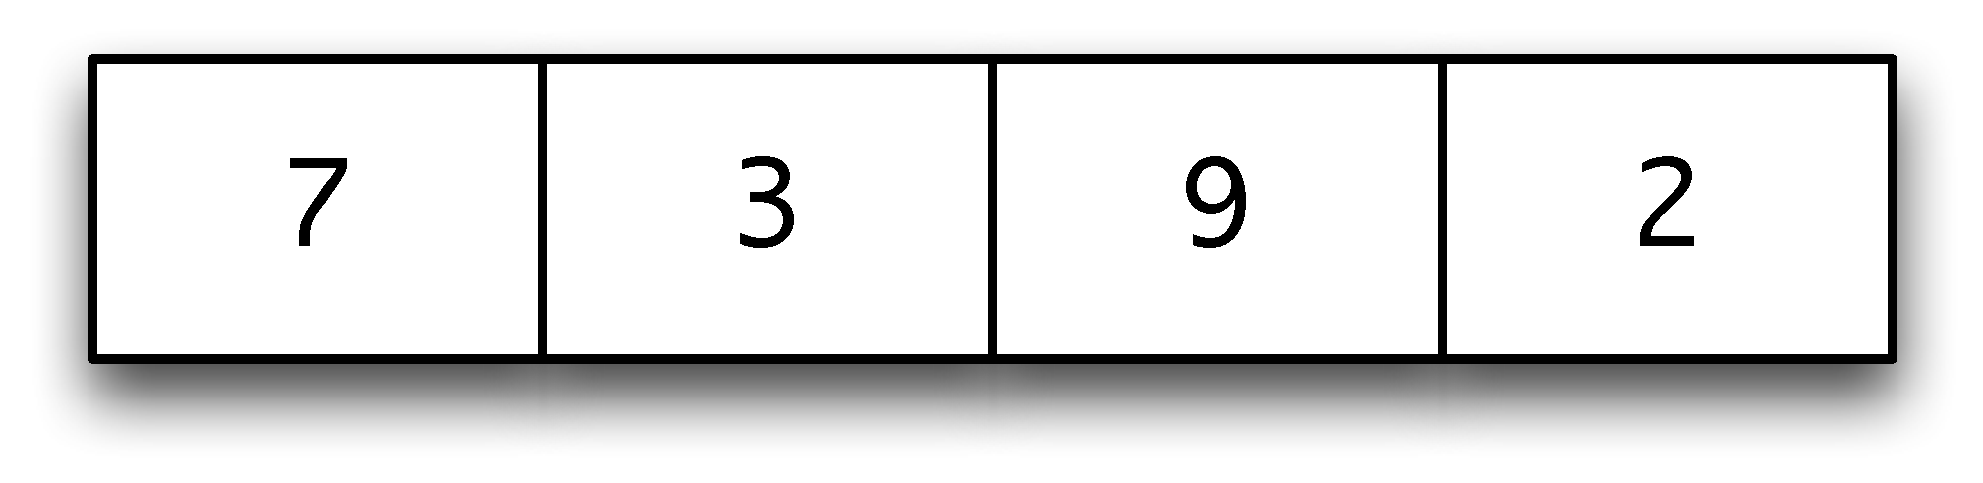
\includegraphics[height=1cm]{Pictures/list1.pdf}\\
is to sort the tail \texttt{[3,9,2]} to give\\
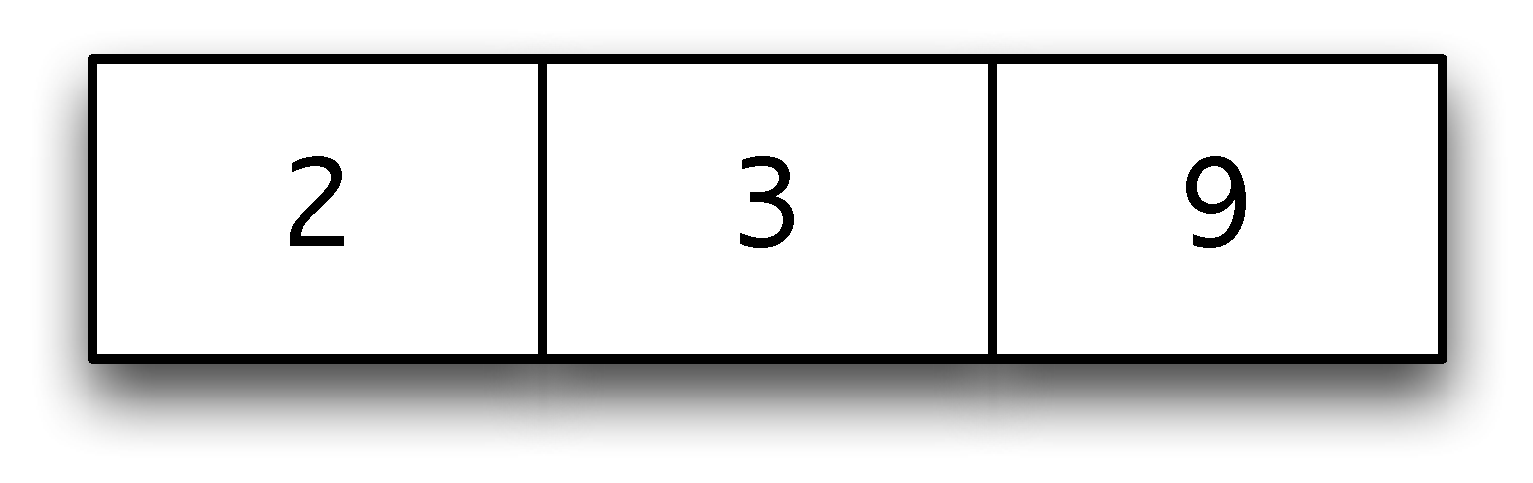
\includegraphics[height=1cm]{Pictures/list2.pdf}\\
It is then a matter of inserting the head, {\mi 7}, in the right place in
this list, to give the result\\
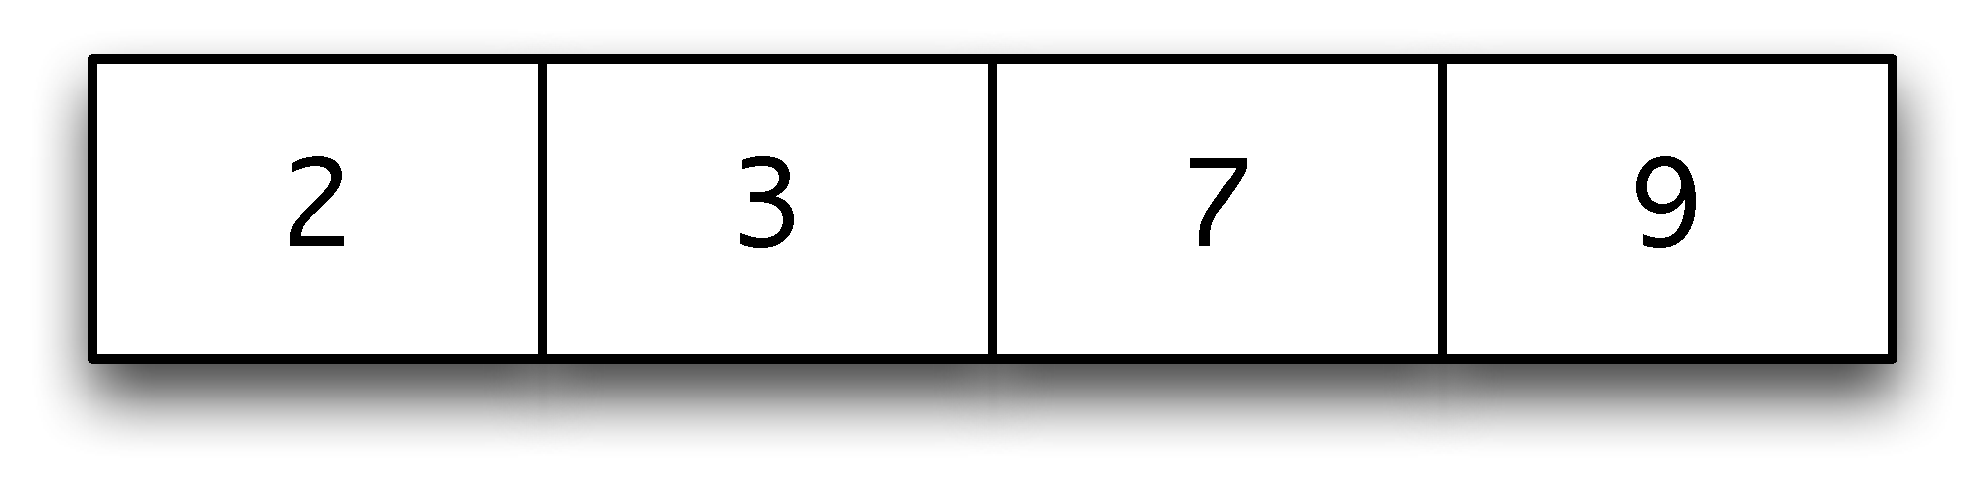
\includegraphics[height=1cm]{Pictures/list3.pdf}\\
This gives the definition of \texttt{iSort} -- the `\texttt{i}' is for
\textbf{ insertion} sort.\index{sorting!insertion}
\begin{alltt}
iSort :: [Integer] -> [Integer]\minx{iSort}
\bl
iSort []     = [] \hfill (iSort.1)
iSort (x:xs) = ins x (iSort xs) \hfill (iSort.2)
\end{alltt}
This is a typical example of top-down\index{design!top-down}
definition, first discussed in Section \ref{designProgram}. We have defined \texttt{iSort}
assuming we can define \texttt{ins}\minx{ins}.
The development of the program has been
in two separate parts, since we have a definition of the function \texttt{iSort}
using a simpler function \texttt{ins}, together with a definition of the
function \texttt{ins} itself. Solving each sub-problem is simpler than
solving the original problem itself.

Now we have to define the function
\begin{alltt}\minx{ins}
ins :: Integer -> [Integer] -> [Integer]
\end{alltt}
To get some guidance about how \texttt{ins} should behave, we look at
some examples. Inserting \texttt{7} into \texttt{[2,3,9]} was given above, while
inserting \texttt{1} into the same list gives\\
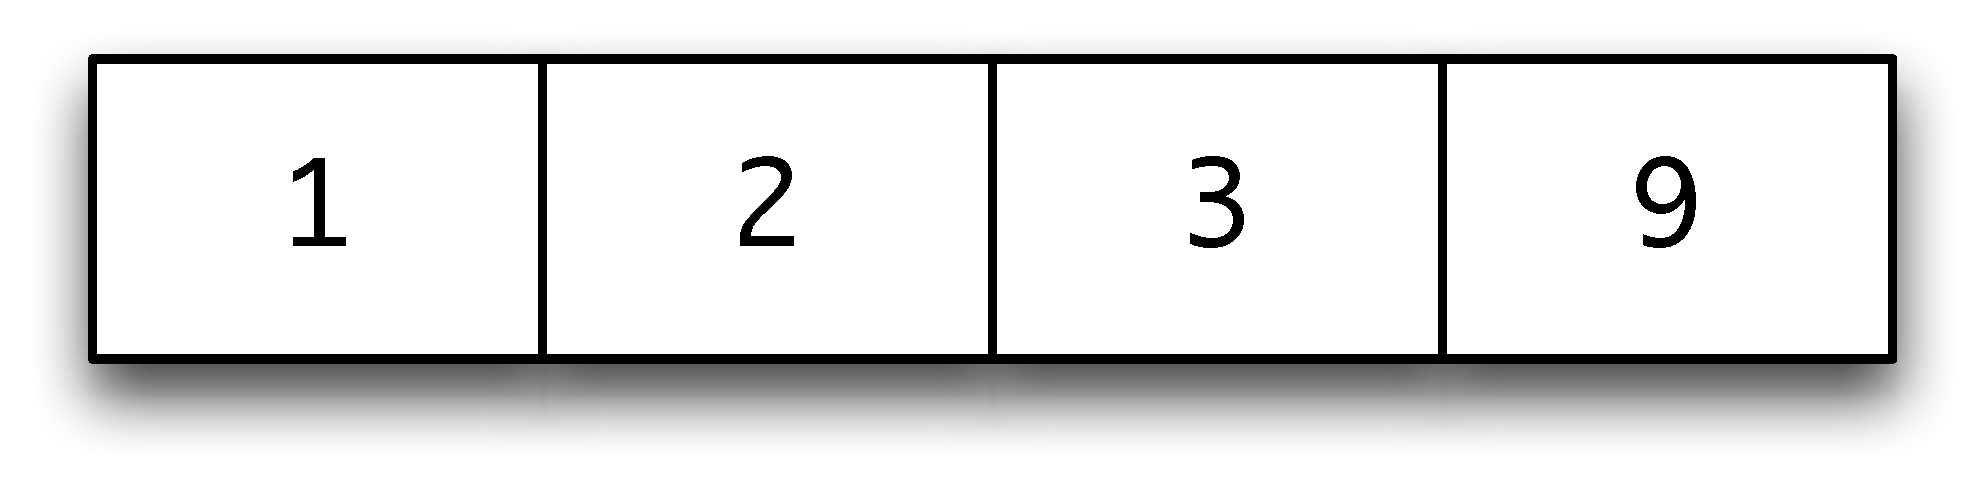
\includegraphics[height=1cm]{Pictures/list4.pdf}\\
Looking at these two examples we see that
\begin{titemize}
\item in the case of \texttt{1}, if the item to be inserted is no larger than
the head of the list, we cons it to the front of the list;
\item In the case of \texttt{7}, if the item is greater than the head, we
insert it in the tail of the list, and cons the head to the result, thus:
\end{titemize}
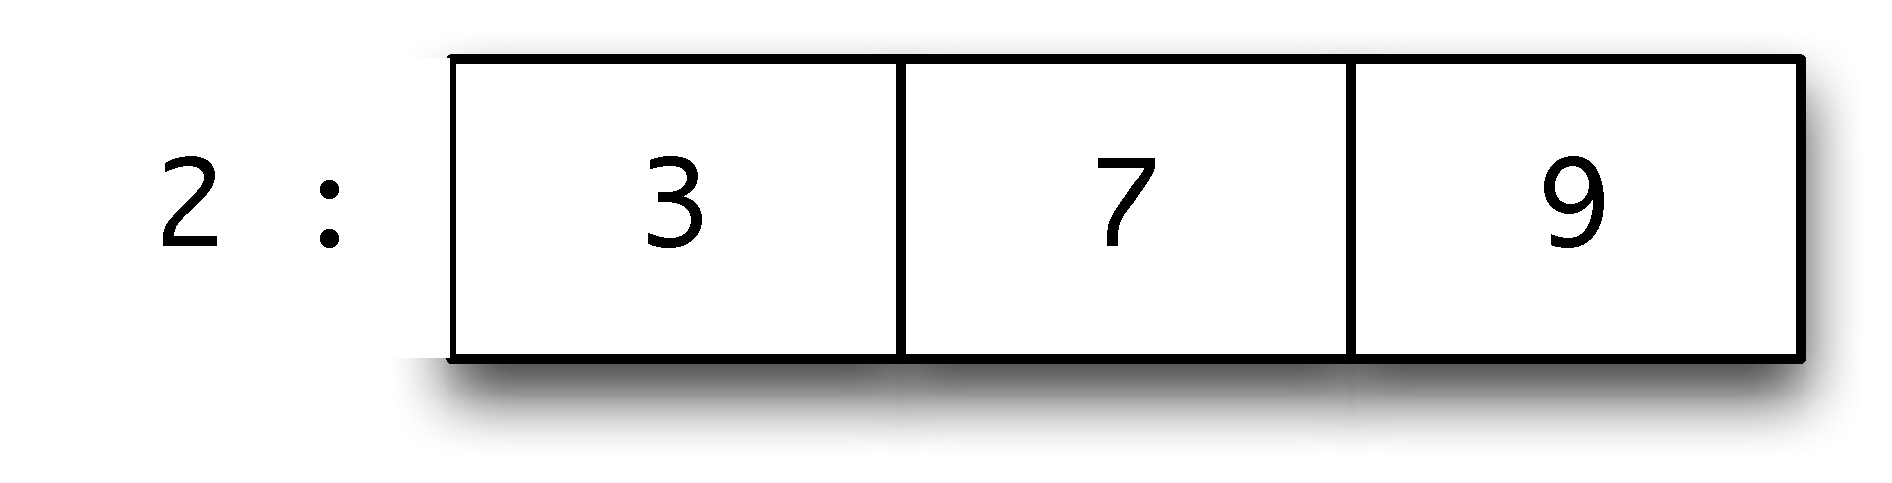
\includegraphics[height=1cm]{Pictures/list5.pdf}\\
The function can now be defined, including the case that the list is empty.
\begin{alltt}
ins x []    = [x] \hfill(ins.1)
ins x (y:ys) 
  | x <= y      = x:(y:ys)\hfill(ins.2)
  | otherwise   = y : ins x ys\hfill(ins.3)
\end{alltt}
We now show the functions in action, in the calculation\index{calculation} 
of \texttt{iSort [3,9,2]}:
\begin{alltt}
iSort [3,9,2]
\step ins 3 (iSort [9,2]) \hfill {\rm by} (iSort.2)
\step ins 3 (ins 9 (iSort [2])) \hfill {\rm by} (iSort.2)
\step ins 3 (ins 9 (ins 2 (iSort []))) \hfill {\rm by} (iSort.2)
\step ins 3 (ins 9 (ins 2 [])) \hfill {\rm by} (iSort.1)
\step ins 3 (ins 9 [2]) \hfill {\rm by} (ins.1)
\step ins 3 (2 : ins 9 []) \hfill {\rm by} (ins.3)
\step ins 3 [2,9] \hfill {\rm by} (ins.1)
\step 2 : ins 3 [9] \hfill {\rm by} (ins.3)
\step 2 : [3,9] \hfill {\rm by} (ins.2)
\step [2,3,9]
\end{alltt}
Developing this function has shown the advantage of looking at examples
while trying to define a function; the examples can give a guide about
how the definition might break into cases, or the pattern of the
recursion. We also saw how using top-down design can break a larger problem
into smaller problems which are easier to solve.

In the next section we look at definitions by more general forms of
recursion.

\index{design!list functions|)}
\index{primitive recursion!list|)}
\index{design!where do I start?|)}
\index{primitive recursion!finding definitions|)}
\end{example}
\begin{exercises}


\item
Test your implementations against the built-in definitions, using the method outlined on page \pageref{qcretest}.


\item Using primitive recursion over lists, define a function
\begin{alltt}
elemNum :: Integer -> [Integer] -> Integer
\end{alltt}
so that \texttt{elemNum x xs} returns the number of times that
\texttt{x} occurs in the list \texttt{xs}. 

Can you define \texttt{elemNum} without using primitive recursion,
using list comprehensions and built-in functions instead?

\item Define a function
\begin{alltt}
unique :: [Integer] -> [Integer]
\end{alltt}
so that \texttt{unique xs} returns the list of elements of \texttt{xs}
which occur exactly once. For example, \texttt{unique [4,2,1,3,2,3]} is
\texttt{[4,1]}. You might like to think of two solutions to this
problem: one using list comprehensions and the other not.

\item 
Can you write a property which links \texttt{elemNum} and \texttt{unique} from the previous two questions? Check to see whether this property does hold using QuickCheck.

\item
Give primitive recursive definitions of the prelude functions
\texttt{reverse} and \texttt{unzip}.


\item Can you use the \texttt{iSort} function to find the minimum and maximum
elements of a list of numbers? How would you find these elements without using
\texttt{iSort}? 

\item
Design test data for the \texttt{ins} function. Your data should address
different possible points of insertion, and also look at any exceptional
cases.

\item
Define a function
\begin{alltt}
isSorted :: [Integer] -> Bool
\end{alltt}
which is true when its argument is sorted in ascending order. How could you use this to write QuickCheck properties to check your \texttt{iSort} and \texttt{ins} functions?

\item {[Harder]}
Is it enough to test that the result of \texttt{iSort} is sorted? What other property should a sorting function have? Can you write a QuickCheck property to check this?


\item
By modifying the definition of the \texttt{ins} function we can change the
behaviour of the sort, \texttt{iSort}. Redefine \texttt{ins} in two different ways
so that 
\begin{titemize}
\item the list is sorted in descending order;
\item duplicates are removed from the list. For example,
\begin{alltt}
iSort [2,1,4,1,2] = [1,2,4]
\end{alltt}
under this definition. 
\end{titemize}

\item
Would you need to redefine your function \texttt{isSorted} to deal with the two different variations of sorting discussed in the last question? If so, how would you modify it; if not, explain why not.

\item
Design test data for the duplicate-removing version of
\texttt{iSort}, explaining your choices.

\item
By modifying the definition of the \texttt{ins} and \texttt{iSort} functions, 
define a function to sort lists of pairs of numbers. The ordering should
be \textbf{lexicographic} -- the dictionary ordering. 
\index{order!lexicographic} This ordering first
looks at the first halves of the pairs; only if these values are equal
are the second halves compared. For instance, \texttt{(2,73)}
is smaller than \texttt{(3,0)}, and this is smaller than \texttt{(3,2)}.
\end{exercises}

\section{General recursions over lists}
\index{general recursion!over lists|(}

Just as we argued in Section \ref{genRecursion}, a recursive definition
of a function need not always use the value of the function
on the tail;  any recursive call to
a value on a {\em simpler\/} list will be legitimate, and so a number of
different patterns of recursion are available for finding function
definitions over lists.
In trying to use recursion over lists to define a function we need to pose the
question:

\subsubsection*{In defining {\tt f (x:xs)} which values
of {\tt f ys} would help me to work out the answer?}

\begin{example}
\subexample*{1.} 
It is possible to use recursion over two arguments simultaneously, 
an example being the definition of the prelude function \texttt{zip}.
Recall that here we turn two lists into a list of pairs,
\begin{alltt}\minx{zip}
zip :: [a] -> [b] -> [(a,b)]
\end{alltt}
with the examples
\begin{alltt}
zip [1,5] ['c','d']     = [(1,'c'), (5,'d')]
zip [1,5] ['c','d','e'] = [(1,'c'), (5,'d')]
\end{alltt}
If each of the lists is non-empty, we form a pair from their heads,
and then zip their tails, giving
\begin{alltt}
zip (x:xs) (y:ys) = (x,y) : zip xs ys\hfill(zip.1)
\end{alltt}
but in all other cases -- that is when at least one of the lists is empty -- 
the result is empty:
\begin{alltt}
zip _ _ = []\hfill(zip.2)
\end{alltt}
Note that we rely on the sequential nature of pattern matching
here;\index{pattern matching!sequentiality of} we can give the patterns
for \texttt{(zip.2)} explicitly if we wish, thus:
\begin{alltt}
zip (x:xs) (y:ys) = (x,y) : zip xs ys
zip (x:xs) []     = []
zip []     zs     = []
\end{alltt}
and in the second definition we see the three separate cases given in
three separate equations. Using the original definition, an example
calculation gives
\begin{alltt}
zip [1,5] ['c','d','e']
\step (1,'c') : zip [5] ['d','e']\hfill\textrm{by }(zip.1)
\step (1,'c') : (5,'d') : zip [] ['e']\hfill\textrm{by }(zip.1)
\step (1,'c') : (5,'d') : []\hfill\textrm{by }(zip.2)
\step (1,'c') : [ (5,'d') ]\hfill\textrm{by defn\ of} :
\step [ (1,'c') , (5,'d') ]\hfill\textrm{by defn\ of} :
\end{alltt}
Note that we have used the fact that `\texttt{:}' is right
associative in writing this calculation.

\subexample*{2.} 
The function \texttt{take} is used to take a given number of values from
a list. For instance, 
\begin{alltt}\minx{take}
take 5  "Hot Rats" = "Hot R"
take 15 "Hot Rats" = "Hot Rats" 
\end{alltt}
In this example we do recursion over an \texttt{Int} and a list
\begin{alltt}
take :: Int -> [a] -> [a]
\end{alltt}
There are some special cases, when the \texttt{Int} is zero, or the list
is empty
\begin{alltt}
take 0 _        = []\hfill(take.1)
take _ []       = []\hfill(take.2)
\end{alltt}
What about the general case, when the list is non-empty and the
\texttt{Int}
greater than zero? We take \texttt{n-1} elements from the tail of the
list, and place the head on the front, thus:
\begin{alltt}
take n (x:xs)
  | n>0         = x : take (n-1) xs\hfill(take.3)
\end{alltt}
and in the other cases we give an error
\begin{alltt}\minx{error}
take _ _        = error "PreludeList.take: negative argument"
\ \hfill(take.4)
\end{alltt}

\subexample*{3.} \index{sorting!quicksort}\index{quicksort}
As a final example, we look at another method for sorting lists (of
integers). The \textbf{quicksort} algorithm works by 
generating {\em two} recursive calls to sort. Suppose we are to sort the
list
\begin{alltt}
                        [4,2,7,1,4,5,6]
\end{alltt}
we can take off the head, \texttt{4}, and then split the result 
\texttt{[2,7,1,4,5,6]} into two parts: 
\begin{alltt}
                        [2,1,4]           [7,5,6]
\end{alltt}
The first contains the elements no larger than \texttt{4}, the
second those exceeding \texttt{4}. We sort these two, giving
\begin{alltt}
                        [1,2,4]           [5,6,7]
\end{alltt}
and then we get an ordered version of the original list thus
\begin{alltt}
                        [1,2,4] ++ [4] ++ [5,6,7]
\end{alltt}
We can write this now
\begin{alltt}
qSort :: [Integer] -> [Integer]

qSort [] = []\hfill(qSort.1)
qSort (x:xs) 
  = qSort [ y | y<-xs , y<=x] ++ [x] ++ qSort [ y | y<-xs , y>x]
\ \hfill(qSort.2)
\end{alltt}
It is striking to see how close this program is to our informal
description of the algorithm, and this expressiveness is one 
of the important advantages of a functional approach.
 
We can see that this recursion will give an answer for every finite
list, since in the recursive calls we apply \texttt{qSort} to two
sublists of \texttt{xs}, which are necessarily smaller than
\texttt{(x:xs)}.


In Chapter \ref{behaviour} we talk about the efficiency of various
algorithms, and show that in general quicksort will be more efficient
than insertion sort.
In the following section we look at a larger example of definitions
which use general forms of recursion.
\end{example}

\begin{exercises}
\item 
Using the definition of \texttt{take} as a guide,
define the prelude functions \texttt{drop} and \texttt{splitAt}. Write QuickCheck tests for these re-defined functions.

\item
What is the value of \texttt{take (-3) []} according to the definition
of \texttt{take} given earlier? How would you modify the definition so
that there is an error reported whenever the \texttt{Int} argument is
negative?


\item
The \texttt{zip} function takes its two arguments separately: we can define this variant to take the arguments as a pair:
\begin{alltt}
zip' :: ([a],[b]) -> [(a,b)]
zip' (xs,ys) = zip xs ys
\end{alltt}
There's a built-in function, which has the reverse effect, taking a list of pairs into a pair of lists:
\begin{alltt}
unzip :: [(a,b)] -> ([a],[b])
\end{alltt}
Write a property for \texttt{zip'} and \texttt{unzip} that expresses that they are the `inverse' of each other: does it matter the order in which they are applied? Try both ways, and see what happens when you apply \texttt{quickCheck} in each case.
 
\item
How would you define a function \texttt{zip3} which zips together three
lists? Try to write a recursive definition and also one which {\em
uses\/} \texttt{zip} instead; what are the advantages and disadvantages
of the two different definitions?

\item
How would you modify \texttt{qSort} to sort a list into descending order?
How would you ensure that \texttt{qSort} removed duplicate elements?

\item
One list is a \textbf{sublist} of another if the elements of the first occur in the
second, in the same order. For instance, \texttt{"ship"} is a sublist
of \texttt{"Fish \& Chips"}, but not of \texttt{"hippies"}.

A list is a \textbf{subsequence} of another if it occurs as a sequence
of elements {\em next to each other}. For example, \texttt{"Chip"} is a
subsequence
of \texttt{"Fish \& Chips"}, but not of \texttt{"Chin up"}.

Define functions which decide whether one string is a sublist or a
subsequence of another string.

\item
Write QuickCheck properties which test your implementations of the tests for `sublist' and `subsequence'.

\end{exercises}

\section{Example: text processing}
\index{examples!text processing|see{text processing}}
\index{text processing|(}
\label{textProc}

In word processing systems it is customary for lines to be filled and
broken automatically, to enhance the appearance of the
text. This book is no exception. Input of the form
\begin{alltt}
{\hskip1pc}The heat bloomed     in December
 as the   carnival  season
            kicked into  gear.
Nearly helpless with sun and glare, I avoided Rio's brilliant
sidewalks
  and glittering beaches,
panting in dark   corners
and waiting out the inverted southern summer.
\end{alltt}
would be transformed by \textbf{filling} to \index{text processing!filling}
\begin{alltt}
{\hskip1pc}The heat bloomed in December as the
carnival season kicked into gear.
Nearly helpless with sun and glare,
I avoided Rio's brilliant sidewalks
and glittering beaches, panting in
dark corners and waiting out the
inverted southern summer.
\end{alltt}
To align the right-hand margin, the text is \textbf{justified} by adding extra
\index{text processing!justification}
inter-word spaces on all lines but the last:
\begin{alltt}
{\hskip1pc}The heat bloomed in December as the
carnival  season  kicked into gear.
Nearly helpless with sun and glare,
I avoided Rio's brilliant sidewalks
and glittering beaches, panting  in
dark  corners  and  waiting out the
inverted southern summer.
\end{alltt}
An input file in Haskell can be
treated as a string of characters, and so string-manipulating operations
play an important role here. Also, since strings are lists, this example
will exercise general list functions.

\subsection*{Overall strategy}

In this section we give an example of bottom-up program development,
thinking first about some of the components we will need to solve the
problem, rather than decomposing the solution in a top-down way.
\index{design!bottom up}

The first step in processing text will be to split an input string into 
\textbf{words}, discarding any white space. The words are then rearranged into
lines of the required length. These lines can then have spaces added so as to
justify the text. We therefore start by looking at how text is split into
\index{text processing!splitting into words}
words. 

\subsection*{Extracting words}

We first ask, given a string of characters, how should we define a
function to take the first word from the front of a string? 

A word is any sequence which does not contain
the \textbf{whitespace} characters space, tab and newline. 
\begin{alltt}
whitespace = ['\bs{n}','\bs{t}',' ']\minx{whitespace}
\end{alltt}
In defining \texttt{getWord} we will use the standard function \texttt{elem},
which tests whether an object is an element of a list. For instance,  
\texttt{elem 'a' whitespace} is \texttt{False}.

To guide the
definition, consider two examples.
\begin{itemize}
\item \texttt{getWord " boo"} should be \texttt{""} as the first character is
whitespace;
\item \texttt{getWord "cat dog"} is \texttt{"cat"}. We get this by putting {\mi
'c'} on the front of \texttt{"at"}, which is \texttt{getWord "at dog"}.
\end{itemize}
The definition is therefore given by:
\begin{alltt}
getWord :: String -> String\minx{getWord}
getWord []    = [] \hfill (getWord.1)
getWord (x:xs) 
  | elem x whitespace   = []\hfill(getWord.2)
  | otherwise           = x : getWord xs\hfill (getWord.3)
\end{alltt}
Consider an example
\begin{alltt}
getWord "cat dog"
\step 'c' : getWord "at dog" \hfill {\rm by} (getWord.3)
\step 'c' : 'a' : getWord "t dog" \hfill {\rm by} (getWord.3)
\step 'c' : 'a' : 't' : getWord " dog" \hfill {\rm by} (getWord.3)
\step 'c' : 'a' : 't' : [] \hfill {\rm by} (getWord.2)
\step "cat"
\end{alltt}
In a similar way, the first word of a string can be dropped.
\begin{alltt}
dropWord :: String -> String\minx{dropWord}
dropWord []    = []
dropWord (x:xs) 
  | elem x whitespace   = (x:xs)
  | otherwise           = dropWord xs
\end{alltt}
It is easy to check that \texttt{dropWord "cat dog" = " dog"}. We aim to
use the functions \texttt{getWord} and \texttt{dropWord} to split a string
into its constituent words. Note that before we take a word from the
string \texttt{" dog"}, we should remove the whitespace character(s) from the
front. The function \texttt{dropSpace} will do this.
\begin{alltt}
dropSpace :: String -> String\minx{dropSpace}
dropSpace []    = []
dropSpace (x:xs) 
  | elem x whitespace   = dropSpace xs
  | otherwise           = (x:xs)
\end{alltt}
How is a string \texttt{st} to be split into words? Assuming \texttt{st} has no
whitespace at the start,
\begin{titemize}
\item the first word in the output will be given by applying \texttt{getWord} to
\texttt{st};
\item the remainder will be given by splitting what remains after removing
the first word and the space following it:
\texttt{dropSpace (dropWord st)}.
\end{titemize}
The top-level function \texttt{splitWords} calls \texttt{split} after removing any
whitespace at the start of the string. 
\begin{alltt}
type Word = String\minx{Word}
\bl
splitWords :: String -> [Word]\minx{splitWords}
splitWords st = split (dropSpace st)
\bl
split :: String -> [Word]
split [] = []
split st
  = (getWord st) : split (dropSpace (dropWord st))
\end{alltt}
Consider a short example.
\begin{alltt}
splitWords "  dog cat"
\step split "dog cat"
\step (getWord "dog cat")
         : split (dropSpace (dropWord "dog cat"))
\step "dog" : split (dropSpace " cat")
\step "dog" : split "cat"
\step "dog" : (getWord "cat")
         : split (dropSpace (dropWord "cat"))
\step "dog" : "cat" : split (dropSpace [])
\step "dog" : "cat" : split []
\step "dog" : "cat" : []
\step [ "dog" , "cat" ]
\end{alltt}

\subsection*{Splitting into lines}

Now we have to consider how to break a list of words into lines. As before,
we look to see how we can take the first line from a list of words. 
\begin{alltt}
type Line = [Word]
getLine :: Int -> [Word] -> Line\minx{getLine}
\end{alltt}
\texttt{getLine} takes two parameters. The first is the length of the line to be
formed, and the second the list from which the words are taken. The definition 
uses \texttt{length} to give the length of a list.
The definition will have three cases
\begin{titemize}
\item In the case that no words are available, the line formed is empty.
\item If the first word available is \texttt{w}, then this goes on the line if
there is room for it: its length, \texttt{length w}, has to be no greater than the
length of the line, \texttt{len}.\\
 The remainder of the line is built from the 
words that remain by taking a
line of length  \texttt{len-(length w+1)}.
\item If the first word does not fit, the line has to be empty. 
\end{titemize}
\begin{alltt}
getLine len []     = []
getLine len (w:ws)
  | length w <= len     = w : restOfLine  
  | otherwise           = []
    where
    newlen      = len - (length w + 1)
    restOfLine  = getLine newlen ws
\end{alltt}
Why is the \texttt{rest} of the line of length \texttt{len-(length w+1)}? Space must
be allocated for the word \texttt{w} {\em and\/} the inter-word space needed to separate
it from the word which follows. How does the function work in an example?
\begin{alltt}
getLine 20 ["Mary","Poppins","looks","like",...
\step "Mary" : getLine 15 ["Poppins","looks","like",...
\step "Mary" : "Poppins" : getLine 7 ["looks","like",...
\step "Mary" : "Poppins" : "looks" : getLine 1 ["like",...
\step "Mary" : "Poppins" : "looks" : []
\step [ "Mary" , "Poppins" , "looks" ]
\end{alltt}
A companion function,
\begin{alltt}
dropLine :: Int -> [Word] -> Line\minx{dropLine}
\end{alltt}
removes a line from the front of a list of words, just as \texttt{dropWord} is a
companion to \texttt{getWord}. The function to split a list of words
into lines of length at most (the constant value) \texttt{lineLen} can now be defined:
\begin{alltt}
splitLines :: [Word] -> [Line]\minx{splitLines}
splitLines [] = []
splitLines ws
  = getLine lineLen ws
         : splitLines (dropLine lineLen ws)
\end{alltt}
This concludes the definition of the function \texttt{splitLines}, which gives
filled lines from a list of words. 

\subsection*{Conclusion}

To fill a text string
into lines, we write
\begin{alltt}
fill :: String -> [Line]\minx{fill}
fill = splitLines . splitWords
\end{alltt}
To make the result into a single string we need to write a function 
\begin{alltt}
joinLines :: [Line] -> String\minx{joinLines}
\end{alltt}
This is left as an exercise, as is justification of lines.
\index{text processing|)}


\begin{exercises}

\item
Define the function \texttt{dropLine}
specified in the text.

\item
Give a definition of the function
\begin{alltt}
{\hskip1pc}joinLine :: Line -> String
\end{alltt}
which turns a line into printable form. For example,
\begin{alltt}
{\hskip1pc}joinLine [ "dog" , "cat" ] = "dog cat"
\end{alltt}

\item
Using the function \texttt{joinLine}, or otherwise, define the function
\begin{alltt}
{\hskip1pc}joinLines :: [Line] -> String
\end{alltt}
which joins together the lines, separated by newlines.

\item
In this case study we have defined separate `take' and `drop' functions for
words and lines.
Redesign the program so that it uses `split' functions -- like the prelude
function \texttt{splitAt} -- instead.

\item
{[Harder]} Modify the function \texttt{joinLine} so that it justifies the
line to length \texttt{lineLen} by adding the appropriate number of spaces
between the words. 

\item
Design a function
\begin{alltt}
{\hskip1pc}wc :: String -> (Int,Int,Int)
\end{alltt}
which when given a text string returns the number of characters, words and
lines in the string. The end of a line in the string is signalled by the
newline character, \texttt{'\bs{n}'}. Define a similar function
\begin{alltt}
{\hskip1pc}wcFormat :: String -> (Int,Int,Int)
\end{alltt}
which returns the same statistics for the text {\em after\/} it has been
filled.

\item
Define a function
\begin{alltt}
{\hskip1pc}isPalin :: String -> Bool
\end{alltt}
which tests whether a string is a palindrome -- that is whether it is the
same read both backwards and forwards. An example is the string
\begin{alltt}
{\hskip1pc}Madam I'm Adam
\end{alltt}
Note that punctuation and white space are ignored in the test, and that no
distinction is made between capital and small letters. You might first like to
develop a test which simply tests whether the string is exactly the same
backwards and forwards, and only afterwards take account of punctuation and
capital letters.

\item
{[Harder]} Design a function
\begin{alltt}
{\hskip1pc}subst :: String -> String -> String -> String
\end{alltt}
so that
\begin{alltt}
subst oldSub newSub st
\end{alltt}
 is the result of replacing the first
occurrence in \texttt{st} of the substring \texttt{oldSub} by the substring \texttt{newSub}. For instance,
\begin{alltt}
{\hskip1pc}subst "much  " "tall " "How much  is that?"
  = "How tall is that?"
\end{alltt}
If the substring \texttt{oldSub} does not occur in \texttt{st}, the result should
be \texttt{st}.

\item {[Harder]} 
Define QuickCheck properties which test the behaviour of your \texttt{subst} function, defined in the previous question.


\index{lists!defining functions|)}
\index{general recursion!over lists|)}
\end{exercises}



\begin{summary}
This chapter has shown how functions can be defined by recursion over lists, and 
completes our account of the different ways that list-processing functions can be defined.
In the chapter we have looked at examples of the design
principles which we first discussed in Chapter \ref{writingProgs},
including `divide and conquer' and general pieces of advice about
designing recursive programs. The text processing case study provides a
broadly bottom-up approach to defining a library of functions. 
\end{summary}

%\end{document}

\chapter{Playing the game: I/O in Haskell}
\chapstart

\label{io}


This chapter completes the design and implementation of the Rock - Paper - Scissors game. We start by looking at how \emph{strategies} can be represented as functions. One of the real strengths of Haskell is to be able to treat functions just like any other data, and strategies are the first time we do that in practice.
 
Next we explore how the simplest kinds of programs, reading and writing
to a terminal, can be developed in Haskell. The model we describe forms
the foundation for more complex interactions like those in a mail system
or an operating system. We start by discussing how in the past I/O has been a problem for the
users of a functional language. 
The solution in Haskell is to 
introduce the types \texttt{IO a}, which we can
think of as \emph{programs} that do some input/output before returning a value
of type \texttt{a}. These programs include simple operations to read and write
information, as well complex programs which are built from a number of 
\texttt{IO} programs
sequenced into one by means of the \texttt{do} construct. 

We conclude the chapter by explaining how to play the Rock - Paper - Scissors game: we show how to play one strategy against another, as well as how you can play interactively against a strategy.

\section{Rock - Paper - Scissors: strategies}
\label{strategiesRPS}\index{Rock - Paper - Scissors|(}

\begin{wrapfigure}[8]{r}{5cm}
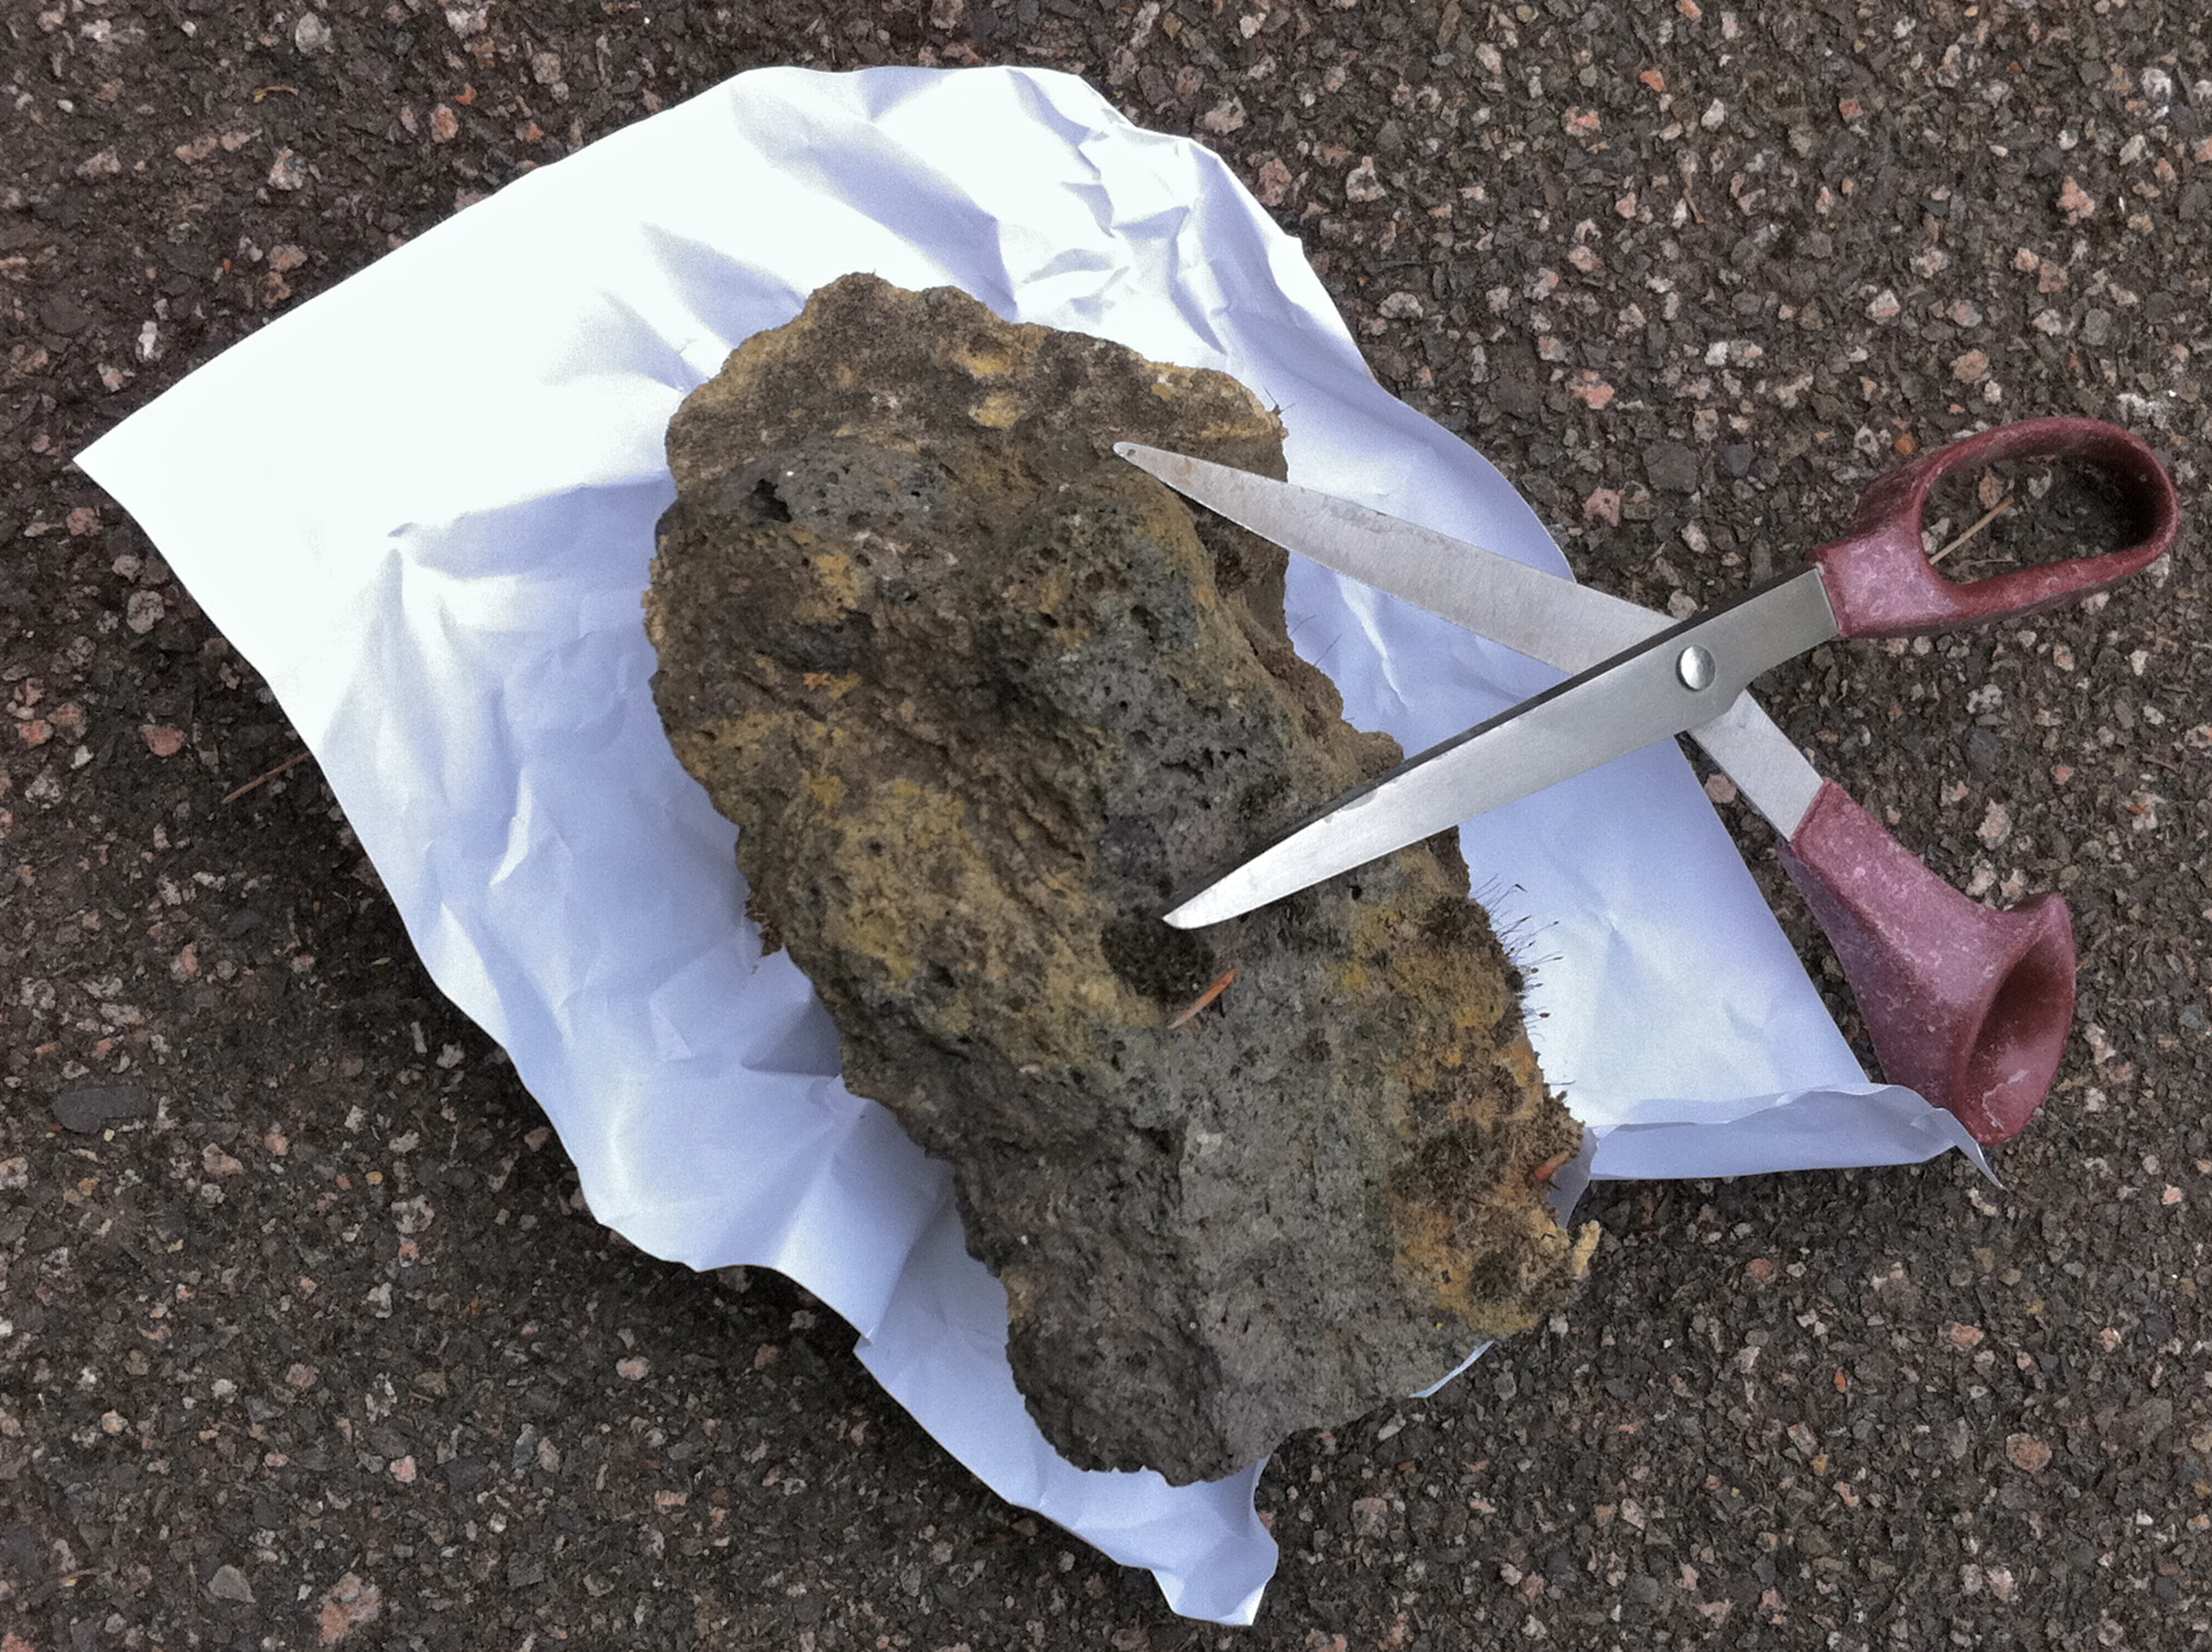
\includegraphics[width=5cm]{Pictures/RPS.pdf}
\end{wrapfigure}
Now that we have seen how to define functions over lists from scratch, as well as making use of functions in the prelude and other libraries, it is time to go back to the discussions of games that we started earlier in the book. In particular, we go back to the Rock - Paper - Scissors game, first introduced in Section \ref{EnumTypes}.

\subsection*{Scoring the moves}

Recall that we defined the \texttt{Move} type like this
\begin{alltt}
data Move = Rock | Paper | Scissors 
            deriving (Show,Eq) 
\end{alltt}
It's worth looking back at that section for definitions of the functions \texttt{beat} and \texttt{lose} as well as the type \texttt{Result} and the function \texttt{outcome} defined in the exercises. 

In that section we were concerned with a single move, but here we want to look at a whole \emph{tournament}, when two players play a sequence of moves against each other.
We can model a tournament by this type definition
\begin{alltt}\minx{Tournament}
type Tournament = ([Move],[Move])
\end{alltt}
where the lists model the moves made by the two players: let's call them A and B. An example tournament is given by
\begin{alltt}
([Rock,Rock,Paper],[Scissors,Paper,Rock])
\end{alltt}

\begin{exercises}

\item
Define a function \label{outcome}
\begin{alltt}
outcome :: Move -> Move -> Integer
\end{alltt}
which gives the outcome as 1, 0, or -1 according to whether the first \texttt{Move} beats, draws with or loses against the second \texttt{Move}. For example, we expect that 
\begin{alltt}
outcome Rock Scissors = 1
\end{alltt}

\item
Using the function \texttt{outcome} that you defined in the previous exercise, define a function
\begin{alltt}
tournamentOutcome :: Tournament -> Integer
\end{alltt}
which gives the outcome of a tournament, giving positive scores to player A, the first player. For example, we should expect
\begin{alltt}
tournamentOutcome ([Rock,Rock,Paper],[Scissors,Paper,Rock]) = 1
\end{alltt}
because the scores for the three rounds are 1, -1 and 1, summing to 1.

\end{exercises}

\subsection*{Strategies}

\index{strategies}

Suppose we want to build a program to play Rock - Paper - Scissors against an opponent. We need to find a way to describe how the machine should play, let's call this a \emph{strategy}. 

We can describe a strategy in words: something like "echo the last move" but that's not a program. Instead we can describe it as a \textbf{function}: the next move that I will play will depend (potentially) on all the moves that my opponent has played, so we can say
\begin{alltt}\minx{Strategy}
type Strategy = [Move] -> Move
\end{alltt}
Remember that \texttt{Strategy} is just shorthand for \texttt{[Move] -> Move}, so when we talk about strategies we are talking about functions that take a list of moves and return a single  `next' move. Let's take a look at some particular strategies now.


\begin{description}

\item[Constant strategy.]
The simplest way of playing is always to play the same thing! So, as strategies we have
\begin{alltt}
rock, paper, scissors :: Strategy 

rock _     = Rock
paper _    = Paper
scissors _ = Scissors
\end{alltt}
Each of these functions ignores its argument and returns the same move in every situation: it should be pretty easy to beat this once an opponent realises what's going on.

\item[Cycle through the possibilities.]
Another option is to cycle through the three possibilities in turn. One way of programming that strategy is this:
\begin{alltt}
cycle :: Strategy

cycle moves
  = case (length moves) `rem` 3 of 
      0 -> Rock
      1 -> Paper
      2 -> Scissors
\end{alltt}
How does this work? We look at the number of moves made so far, which is given by \texttt{length moves}; the remainder on dividing this by 3 cycles through 0, 1, 2 and we use a \texttt{case} expression to map these results to the three options \texttt{Rock}, \texttt{Paper}, \texttt{Scissors}.

\item[A random choice.]
We can make a random choice of play. 
\begin{alltt}
randomStrategy :: Strategy
\end{alltt}
This isn't really a proper function, in fact, because it doesn't always return the same result, we should program this using monads, as described in Chapter \ref{actions}. However, a little bit of `under the hood' work allows us to fake this in Haskell; the details are in the code for this chapter. We'll discuss the full implementation in Section \ref{furtherIO}.

\item[Echo the last move.]\label{echoStrat}
Given the list of moves made by our opponent, it's easy to play by echoing their last move. However, we have to think about one thing first: how are the moves listed in the list of moves: it could be `latest first', or `oldest first'. It's actually convenient to choose \textbf{latest first}, so that the list of moves
\begin{alltt}
[Rock,Rock,Paper]
\end{alltt}
says that \texttt{Paper} was played first, followed by two \texttt{Rock} moves. With this settled we can define the `echo' strategy:
\begin{alltt}
echo :: Strategy

echo (latest:rest) = latest
echo []            = Rock
\end{alltt}
We've had to say what is the response when there are \textbf{no} previous moves, and here we've made the arbitrary choice of \texttt{Rock}.

\item[More strategies.]
More strategies are described in the exercises, giving you a chance to code them as functions of type \texttt{Strategy} for yourself.  

\end{description}

\beware{Using functions as data}{This is an important example, and shows something that's really distinctive about functional programming, because it uses functions to model data in a completely natural way. One way to see this is to try to model strategies \emph{without} using functions: give it a try with the examples here and also those in the exercises, and you'll see that it's not possible to do it in as general a way as functions do!

\medskip
We'll talk more about functions as data and how they can be the input to and output from  other functions, called \emph{higher-order functions} in Chapters \ref{gen2} and \ref{developingHOPs}.
}

\begin{exercises}

\item
Define a strategy which plays the move which would have won against the opponent's last move. Define a strategy which plays the move which would have \emph{lost} against the opponent's last move. Which of these do you think will be a better strategy in practice? Explain your answer.

\item
Define a strategy which plays a random choice \emph{except} when the opponent's last two moves have been the same one. In this case we guess that her next move will not be the same: how does that help? Well, if we know that she's only got two choices, we can play \emph{not to lose}. 

Take the concrete example of \texttt{Rock} being played twice by our opponent. We guess that her next move will be \texttt{Paper} or \texttt{Scissors}: what should we play? The answer is \texttt{Scissors}, because then we'll win if she plays \texttt{Paper} or draw if she also plays \texttt{Scissors}!

\item
Define a strategy which looks at the frequencies that the opponent has played the three choices. If you assume they are making random plays, then why not predict they are about to play the least frequent, and use the trick from the previous exercise to make a choice.

\item {[Harder]}
Go to the World RPS website -- see the box at the end of this section -- to find out more strategies, and try to implement them.

\item {[Harder]}
Define a function 
\begin{alltt}
alternate :: Strategy -> Strategy -> Strategy
\end{alltt}
so that the strategy given by
\begin{alltt}
alternate str1 str2
\end{alltt}
is to combine the two strategies \texttt{str1} and \texttt{str2}, using them alternately.

\item {[Hard]}
Can you write a function which will \emph{analyse} an arbitrary strategy to work out what it does? You will need to think about how to represent this result: is it a string describing what the strategy does, or something a bit less informal?

\item {[Hard]}
Can you use the facilities of QuickCheck -- described in more detail in Section \ref{qcGens} -- to help to analyse what an arbitrary strategy does?

\end{exercises}



\beware{More information about Rock - Paper - Scissors }
{In fact the choice of the first move in defining \texttt{echo} is not completely arbitrary: men are most likely to choose \texttt{Rock} first. This and lots more information about Rock - Paper - Scissors can be found at the World RPS Society website:
\begin{alltt}
http://www.worldrps.com/
\end{alltt}
} 

\index{Rock - Paper - Scissors|)}


\section{Why is I/O an issue?}
\label{ioCaution}\index{I/O|(}
\index{I/O!history}

A functional program consists of a number of definitions, such as
\begin{alltt}
val :: Integer
val = 42

function :: Integer -> Integer
function n = val + n
\end{alltt}
The effect of these definitions is to associate a fixed value with each
name; in the case of \texttt{val} the value is an integer and in the case of
\texttt{function} it is a function from integers to integers.
How is an input or an output action to fit
into this model? 

One approach, taken in Standard ML \shortcite{defsml2e} and F\# \cite{Fsharp}, for instance,
is to include operations like
\begin{alltt}
inputInt :: Integer
\end{alltt}
whose effect is to read an integer from the input; the value read in becomes the value 
given to \texttt{inputInt}.
Each time \texttt{inputInt} is evaluated it will be given a new value, 
and so it is not a fixed integer value as it ought to
be according to our original model.

Allowing this operation into our language 
may not seem to cause too big a problem, but examining the example of
\begin{alltt}
inputDiff = inputInt - inputInt\hfill(inputDiff)
\end{alltt}
shows how it has two important consequences for our model of functional programming. 
\begin{itemize}
\item Suppose that the first item input is \texttt{4}, and that the next
is \texttt{3}. Depending upon the order in which the arguments to
`\texttt{-}' are evaluated, the value of \texttt{inputDiff} will be
either \texttt{1} or \texttt{-1}.
\item More seriously, \texttt{(inputDiff.1)} breaks the model of
reasoning which we have used. Up to now we would have thought that
subtracting a value from itself would have given a result of \texttt{0}, but that is
{\em not\/} the case here. 
\itempar
The reason for this is precisely that the meaning of an expression is
no longer determined by looking only at the meanings of its parts, since we cannot 
give a meaning to
\texttt{inputInt} without knowing where it occurs in a program; as we
saw in the previous point, the first and second occurrences of
\texttt{inputInt} in
\texttt{inputDiff} will generally have different values.
\end{itemize}
As the second point shows, if we take this approach then it will be
substantially more difficult to understand the meaning of any program. 
This is because {\em any\/} definition in a
program may be affected by the presence of the I/O operations. An
example is the function
\begin{alltt}
funny :: Integer -> Integer
funny n = inputInt + n
\end{alltt}
from whose definition we can see the dependence on I/O, but potentially
any function may be affected in a similar way.

Because of this, I/O proved to be a thorny issue for functional programmers
for some considerable time, and there have been a number of attempts to find the right
model for I/O -- indeed, earlier versions of Haskell included two of
these. An illuminating history and overview of functional I/O is given in
\citeN{gordon-book}. 

In this chapter we introduce the basics of I/O using the \texttt{IO} types; Chapter \ref{actions}  describes the \emph{monadic} approach to programming which underlies I/O and other forms of interaction with the `world outside'. 

\section{The basics of input/output}
\label{basicsIO}
\index{I/O!basics|(}



In
thinking about input/output\index{input/output|see{I/O}}\index{IO|see{I/O}} 
or \textbf{I/O} it makes more sense
to think of \emph{actions happening in sequence}. For instance, first
some input might be read,
and then on the basis of that some further input might be read, or output might be 
produced. 

Haskell provides the types \texttt{IO a}\minx{IO}
of \textbf{I/O actions} of type \texttt{a}\index{action, I/O} or \textbf{I/O programs} of type
\texttt{a}. An object belonging to \texttt{IO a}
is a \emph{program} which will do some I/O and then return a value of type
\texttt{a}. Built into Haskell are some primitive I/O programs, as well
as a mechanism to sequence these I/O programs. 

One way of looking
at the \texttt{IO a} types is that they provide a small \emph{imperative
programming \index{I/O!imperative programs}
language} for writing I/O programs on top of Haskell, without compromising the functional
model of Haskell itself.\footnote{The language is unusual in that it is \emph{single assignment}, like Erlang \cite{progErlang,erlangProg}; we'll explain this when we discuss the examples.}

We start by looking at the basic \texttt{IO} capabilities built into the standard prelude, and then we look at a whole lot of examples to see how to put these components together using the
\texttt{do} notation. In the next section we look at how to write `functional loops' to form more complex I/O programs.




\subsection*{Reading input}
\index{I/O!input}

The operation which reads a line of text from the standard input does some I/O and
returns a \texttt{String} which is the line just read. According to the
explanation above, this should be an object of type \texttt{IO String}, and
indeed, the built-in function 
\begin{alltt}\minx{getLine}
getLine :: IO String\minx{getLine}
\end{alltt}
reads a line from the standard input. In a similar way, 
\begin{alltt}
getChar :: IO Char\minx{getChar}
\end{alltt}
will read a single character from the input.

\subsection*{The one-element type}
\index{type!one element}

Haskell contains the type \texttt{()}, which contains one element only.
This element is also written \texttt{()}. A value of this type can convey no useful
information  and so the type is not often used. However, it {\em is\/} useful
in performing \texttt{IO}, as there are cases of IO programs
whose only significance is their I/O actions and not the results they return.
Programs of that sort will have type
\begin{alltt}
IO ()\minx{()}
\end{alltt}
and they will return the value \texttt{()} as their result.


\subsection*{The \texttt{Main} module and the \texttt{main} program}
\minx{Main}\minx{main}

If we compile a Haskell project using GHC, the Glasgow Haskell Compiler, then this produces executable program which runs the function
\begin{alltt}
main :: IO t
\end{alltt}
for some type \texttt{t}: often this is \texttt{()}, so that
\begin{alltt}
main :: IO ()
\end{alltt}
By default, this \texttt{main} program is expected to be in the \texttt{Main} module, but it can be given in any module from the project.


\subsection*{Writing \texttt{Strings}}
\index{I/O!output}

The operation of writing the string \texttt{"Hello, World!"} will be an
object which performs some I/O, but which has nothing of significance to
pass back to the program. It is therefore of type \texttt{IO ()}. 

The general operation to print a text string will be a 
\textbf{function} which
takes the string to be written, and gives back the I/O object which writes
that string:
\begin{alltt}
putStr :: String -> IO ()\minx{putStr}
\end{alltt}
and using this we can write our `hello, world' program.
\begin{alltt}\minx{helloWorld}
helloWorld :: IO ()
helloWorld = putStr "Hello, World!"
\end{alltt}
Using \texttt{putStr} we can define a function to write a line of output.
\begin{alltt}
putStrLn :: String -> IO ()\minx{putStrLn}
putStrLn = putStr . (++ "\bs{n}")
\end{alltt}
The effect of this is to add
a newline to the end of its input before passing it to
\texttt{putStr}.

\subsection*{Writing values in general}

The Haskell prelude provides the class \texttt{Show}
with the function
\begin{alltt}\minx{Show}
show :: Show a => a -> String
\end{alltt}
which can be used to write values of many types. For example, we
can define a general print function from the standard prelude thus
\begin{alltt}\minx{print}
print :: Show a => a -> IO ()
print = putStrLn . show
\end{alltt}

\subsection*{Returning a value: \texttt{return}}
\index{I/O!returning a value}
\minx{return}

Suppose we want to write an I/O action which does no I/O but does return
a value -- we will see examples of this in due course. This is achieved 
by the built-in function
\begin{alltt}
return :: a -> IO a
\end{alltt}
The effect of \texttt{return x} is to do no I/O, but simply to return the
result \texttt{x}. 

If we're writing a program of type \texttt{IO ()} then \texttt{return ()} has the effect of a `\texttt{skip}' in a traditional language: it's a command that does nothing. We use this in cases where we only want to perform an action when a condition holds, like this:
\begin{alltt}
if condition
  then action
  else return ()
\end{alltt}




\subsection*{Running an I/O program}
\index{I/O!running a program}

We have written a simple I/O program, namely \texttt{helloWorld}; how is
it run? In GHCi we can evaluate it at the prompt:
\begin{alltt}\minx{main}
\textsl{Main>} helloWorld
\textsl{Hello, World!}
\textsl{Main>} ...
\end{alltt}
Strictly speaking, the \texttt{main} definition of a Haskell
program should be of type \texttt{IO a} for some \texttt{a}. In GHCi, if
we ask to evaluate an expression \texttt{e} of type \texttt{b}
then it is wrapped up as an object of type \texttt{IO ()} by applying
the
\texttt{print} function.
\medskip

\noindent This completes our introduction to the basic I/O functions in the standard
prelude as well as the method by which \texttt{IO} programs are run.

Next we look at how programs are sequenced, and also how to use the values read in
by means of input programs like
\texttt{getLine}; this is the topic of the next section. 
\index{I/O!basics|)}

\section{The \texttt{do} notation}
\markright{The \texttt{\runinghead do} notation}
\index{sequencing|see{\texttt{do}}}
\index{do@\texttt{do} notation}
\index{I/O!\texttt{do} notation|(}

The \texttt{do} notation gives us a way of building IO programs from the components that we discussed in the previous section. The \texttt{do} notation supports two things:
\begin{itemize}
\item
it is used to \emph{sequence} I/O programs, and
\item
it is used to \textbf{name}\footnote{or `capture' or `bind'} the values returned by \texttt{IO} actions; this means that the later actions can depend on values captured earlier in the program.
\end{itemize}
Together these ideas make a \texttt{do} expression appear like a
simple imperative program, containing a sequence of commands and
assignments; although this analogy is not complete -- we examine how it
breaks down in the next section -- it shows that the model of I/O given
by the \texttt{IO} types is a familiar one, albeit in a different guise.

\subsection*{Sequencing I/O actions}

One purpose of the \texttt{do} construct is to sequence I/O actions 
and we show how it is used through a series of examples.
\begin{example}
\subexample*{1.} 
We begin by looking at
the definition of \texttt{putStrLn} from the standard
prelude. The effect of \texttt{putStrLn str} is to do two things: first
the string \texttt{str} is output, then a newline. This is accomplished
by
\begin{alltt}\minx{putStrLn}
putStrLn :: String -> IO ()

putStrLn str = do putStr str
                  putStr "\bs{n}"
\end{alltt}
Here we see the effect of \texttt{do} is to sequence a number of
\texttt{IO} actions into a single action. The syntax of \texttt{do} is
governed by the offside rule, and \texttt{do} can take any number of
arguments. We see an example of more arguments next.

\subexample*{2.} 
We can write an I/O program to print something four times. The first
version of this is 
\begin{alltt}
put4times :: String -> IO ()

put4times str 
  = do putStrLn str
       putStrLn str
       putStrLn str
       putStrLn str
\end{alltt}


\subexample*{3.} 
So far, we have only seen examples of output, but we can also make inputs a
part of a sequence of actions. For instance, we can read two lines of input and
then output the message \texttt{"Two lines read."}\ thus:
\begin{alltt}
read2lines :: IO ()

read2lines 
  = do getLine
       getLine
       putStrLn "Two lines read."
\end{alltt}
and by analogy with Example 3 it is not difficult to see that we could
write an I/O program which reads an arbitrary number of lines.

\end{example}
\subsection*{Capturing the values read}
\index{I/O!capturing values read}

As was apparent in Section \ref{ioCaution}, it is necessary to be careful in the
way that the results of input actions are handled. The operation
\texttt{inputInt ::\ Integer} was shown to be too powerful to fit into the
functional model, but some mechanism to handle input values is required. This is the
second purpose of the \texttt{do} notation; it is only possible to use the result of an
input within a \texttt{do} expression, and this limitation prevents the
I/O actions from `contaminating' the whole program. 

The sequence of examples continues by examining this aspect of the \texttt{do} notation. 


\begin{example}
\vspace{-5pt}

\subexample*{4.} 
The last example read two lines, but did nothing with the results of the
\texttt{getLine} actions. How can we use these lines in the remainder of
the I/O program? As part of a \texttt{do} program we can \textbf{name}
the results of \texttt{IO a} actions. A program to read a line and then
write that line is given by\minx{<-}
\begin{alltt}\minx{getNput}
getNput :: IO ()

getNput = do line <- getLine
             putStrLn line
\end{alltt}
where the `\texttt{line <-}' names the result of the \texttt{getLine}.

If you are familiar with imperative programming you can think of this as
like an assignment to a variable, as in \index{assignment!and \texttt{<-}}
\begin{alltt}
line := getLine
\end{alltt}
but you should be aware that there are important differences between the
names in a Haskell I/O program and the variables in an imperative
program. The essential difference is that each `\texttt{var <-}' creates a 
{\em new\/} variable \texttt{var}, and so the language 
permits `\textbf{single} assignment'\index{assignment!single}
rather than the
`updatable assignment' familiar from the vast majority of modern imperative languages;
we look at an example of the different in the exercises for Section \ref{ioIter}.

\subexample*{5.} 
We are not forced simply to output the lines we have read, unchanged, so
that we might define
\begin{alltt}
reverse2lines :: IO ()

reverse2lines
  = do line1 <- getLine
       line2 <- getLine
       putStrLn (reverse line2)
       putStrLn (reverse line1)
\end{alltt}
In this example, we read two lines, and then write them in the
opposite order, reversed.
\end{example}
\subsection*{Local definitions in a \texttt{do} expression}
\index{I/O!local definitions}
\index{do@\texttt{do} notation!local definitions}

The notation \texttt{var <- getLine} names the output of the
\texttt{getLine}, and
so acts like a definition. It is also possible to make local definitions
within a \texttt{do}
expression so that we can revisit the last example, as follows.

\subsection*{Example}
\subexample*{6.} 
Example 5 can be redefined to contain local definitions of the reversed lines
\begin{alltt}\minx{let}
reverse2lines :: IO ()

reverse2lines
  = do line1 <- getLine
       line2 <- getLine
       let rev1 = reverse line1
       let rev2 = reverse line2
       putStrLn rev2
       putStrLn rev1
\end{alltt}

\subsection*{Reading values in general}

Haskell contains the class \texttt{Read}
with the function\minx{read}
\begin{alltt}
read :: Read a => String -> a
\end{alltt}
which can be used to parse a string representing a value of a particular
type into that value. 

\subsection*{Example}
\subexample*{7.} 
As an example,
suppose that we want to write an I/O program to read in an integer
value.
To read an integer from a line of input we start by saying 
\begin{alltt}
do line <- getLine
\end{alltt}
but then we need to sequence this with an I/O action to return the \texttt{line}
interpreted as an \texttt{Integer}.
We can convert the \texttt{line} to an integer by the expression
\begin{alltt}
read line :: Integer
\end{alltt}
What we need is the \texttt{IO Integer} action which returns
this value -- this is the purpose of \texttt{return} introduced in the previous section.
Our program to read an \texttt{Integer} is therefore
\begin{alltt}\minx{getInt}
getInt :: IO Integer

getInt = do line <- getLine
            return (read line :: Integer)
\end{alltt}

\begin{summary}
This section has shown that a \texttt{do}
expression provides a context in which to do sequential programming.
It is possible to program complicated I/O interactions, by
sequencing simpler
I/O programs. Moreover, the `\texttt{<-}' allows us to name the value returned 
by an action
and then to use this named value in the remainder of the I/O program. 
It is also possible to make these
programs more readable by judicious use of \texttt{let} definitions
to name intermediate calculations.

In the next section we look at how to write repetitive I/O programs, 
reading all the lines
in the input, for example. We shall see that this can be done by
defining a looping construct recursively. We also discuss the way in
which `\texttt{<-}' behaves differently from the usual assignment
operator.
\index{I/O!\texttt{do} notation|)}
\end{summary}

\begin{exercises}

\item
Write an I/O program which will read a line of input and test whether the
input is a palindrome. The program should
`prompt' for its input and also
output an appropriate message after testing.

\item
Write an I/O program which will read two integers, each on a separate line, and return
their sum. The program should prompt for input and explain its output. 


\item
Define a function
\begin{alltt}
putNtimes :: Integer -> String -> IO ()
\end{alltt}
so that the effect of \texttt{putNtimes n str} is to output \texttt{str}, a string,  \texttt{n} times, one per line.

\item
Write an I/O program which will first read a positive integer,
\texttt{n} say, and then read \texttt{n} integers and write their sum. 
The program should prompt appropriately for its inputs and explain its output. 

\end{exercises}
\section{Loops and recursion}
\label{ioIter}
\index{I/O!loops and recursion}

In this section we examine how to build I/O programs with a repetitive
nature; again we do this by working through a series of examples, concluding with a general pattern for recursive IO programs. 
In particular we program a number of different variations of a function to copy lines from input to output.

\begin{example}

\subexample*{8.} The simplest copying program loops forever:
\begin{alltt}\minx{copy}
copy :: IO ()

copy =
    do line <- getLine 
       putStrLn line
       copy
\end{alltt}
The effect of \texttt{copy} is to read a line, and name the result \texttt{line}; in the next step this is output, and the final `command' is to call \texttt{copy} again, so looping forever. This can be run within GHCi simply by typing \texttt{copy}; it can be interrupted by typing \texttt{Ctrl-C}. 

Programs like this where the only recursive call to the function is the last statement in the \texttt{do} block are called \textbf{tail recursive}. Typically tail recursive functions are efficient to implement, because they resemble a loop in an imperative language.

\subexample*{9.} We can control the number of lines that are copied by passing the number as a parameter:
\begin{alltt}\minx{copyN}
copyN :: Integer -> IO ()

copyN n =
    if n <= 0
    then return ()
    else do line <- getLine
            putStrLn line
            copyN (n-1)
\end{alltt}
The effect of \texttt{copyN 3} should be to copy three lines of input to output. In general, if the number of lines to be copied is less then or equal to zero -- the \texttt{then} branch -- the program just returns \texttt{()}, which does no IO. On the other hand, in the \texttt{else} branch we read a line, print it out, and then call \texttt{copyN (n-1)}.

The \texttt{Integer} variable here is sometimes called the \textbf{loop data} and the value of the loop data is usually modified in the tail recursive call. You can think of the value of the data as like the value of a variable in an imperative language: in this case the value decreases by one at each call, and so we `count down' to the base case where the program terminates.

\subexample*{10.} We can also control the termination of the loop by a condition on the data; we will copy lines until an empty line is encountered.
\begin{alltt}\minx{copyEmpty}
copyEmpty :: IO ()

copyEmpty =
    do line <- getLine 
       if line == ""
          then return ()
          else do putStrLn line
                  copyEmpty
\end{alltt}
Here we first get a line from the input, and call it \texttt{line}. If it is empty we terminate -- just as we did in the last example -- by calling \texttt{return ()}. If it is not empty, we output the line, and tail-recursively call \texttt{copyEmpty}.

\subexample*{11.}
Putting together what we saw in examples 9 and 10, we can \emph{count} the number of lines that we have copied, outputting this when we reach an empty line:
\begin{alltt}\minx{copyCount}
copyCount :: Integer -> IO ()

copyCount n =
    do line <- getLine 
       if line == ""
          then putStrLn (show n ++ " lines copied.")
          else do putStrLn line
                  copyCount (n+1)
\end{alltt}
This behaves like example 10, except that we use the loop data to keep track of the number of lines copied. We can see this in action here:
\begin{alltt}
\textsl{*RPS>} copyCount 0
foo
foo
bar
bar

\textsl{2 lines copied.}
\end{alltt}

\end{example}

We will now look at how these ideas can be used to program a Rock - Paper - Scissors tournament.

\begin{exercises}

\item
Define a \texttt{wc} function which copies input to output until an empty line is read. The program should then output the number of lines, words and characters that have been copied. [\texttt{wc} is a standard unix command line program.]

\item
Define an interactive palindrome checker. You should neglect capitalisation, white space and punctuation, so that
\begin{alltt}
Madam I'm Adam.
\end{alltt}
is recognised as a palindrome.

\item
Write a program which repeatedly reads lines and tests whether they are
palindromes until an empty line is read. The program should explain
clearly to the user what input is expected and output is produced.

\item
Write a program which repeatedly reads integers (one per line) until finding
a zero value and
outputs the sum of the inputs read. 
\item
Write a program which repeatedly reads integers (one per line) until finding
a zero value and
outputs a sorted version of the inputs read. Which sorting algorithm is
most appropriate in such a case?


\item
Explain the behaviour of this \texttt{copy} program
\begin{alltt}
copy :: IO ()

copy =
    do
      line <- getLine
      let whileCopy = 
              do
                if (line == "")
                  then (return ())
                  else 
                    do putStrLn line
                       line <- getLine
                       whileCopy 
      whileCopy
\end{alltt}
where the definition of \texttt{whileCopy} is modelled on a \texttt{while} loop in a traditional programming language.
\end{exercises} 






\section{Rock - Paper - Scissors: playing the game}
\label{playingRPS}\index{Rock - Paper - Scissors|(}

In this section we look at how to play the Rock - Paper - Scissors game, both interactively and by playing one strategy off against another.

\subsection*{Playing interactively}

You can play interactively against a particular strategy using the function
\begin{alltt}\minx{play}
play :: Strategy -> IO ()
\end{alltt}
so that \texttt{play rock} allows you to play against the strategy which always plays \texttt{Rock}. More interesting to play against is 
\begin{alltt}
randomPlay :: IO ()
\end{alltt}
which makes a random choice of strategy for you to play against: this is much more of a challenge to play! A typical example in action is shown here, where you jusy have to hit a single key -- \texttt{r}, \texttt{p}, \texttt{s} or \texttt{R}, \texttt{P}, \texttt{S} -- to play:
\begin{alltt}
\textsl{*RPS>} randomPlay
r
\textsl{I play: p you play: r}
p
\textsl{I play: r you play: p}
s
\textsl{I play: s you play: s}
r
\textsl{I play: s you play: r}
p
\textsl{I play: r you play: p}
s
\textsl{I play: p you play: s}
s
\textsl{I play: r you play: s}
p
\textsl{I play: p you play: p}
r
\textsl{I play: r you play: r}

\textsl{You won: well done!}
\end{alltt}
where the `I' is the machine, and the `you' is the player. 
So, how do we define these functions? The top-level definition is 
\begin{alltt}\minx{play}
play :: Strategy -> IO ()

play strategy =
    playInteractive strategy ([],[])
\end{alltt}
where the worker function, \texttt{playInteractive} is defined like this:
\begin{alltt}\minx{playInteractive}
playInteractive :: Strategy -> Tournament -> IO ()

playInteractive s t@(mine,yours) =
    do 
      ch <- getChar
      if not (ch `elem` "rpsRPS") 
        then showResults t 
        else do let next = s yours 
                putStrLn ("\bs{n}I play: " ++ show next ++ 
                          " you play: " ++ [ch])
                let yourMove = convertMove ch
                playInteractive s (next:mine, yourMove:yours)
\end{alltt}
The pattern here is just like the functions defined in Section \ref{ioIter}: the function is tail recursive, and the \emph{loop data} is of \texttt{Tournament} type, and  represents what has happened in the tournament so far as a pair of lists. The function is called with the lists \texttt{(mine,yours)}; in the recursive call the current plays are added to give \texttt{(next:mine, yourMove:yours)}; remember  here that the latest plays go at the \emph{head} of the list.

So, what does the function do in detail? We read a character, and call the result of the  read \texttt{ch}. If that's not one of the playing characters we show the results of the tournament (see below); if it is one, we calculate what the computer should play, by applying its strategy \texttt{s} to the list of moves so far, we output what the two moves have been, and then we call the function recursively with new loop data,
\begin{alltt}
(next:mine, yourMove:yours)
\end{alltt}
This completes the implementation of the interactive Rock - Paper - Scissors game.

\begin{figure}[t]\index{do@\texttt{do} notation!local definitions}
\beware{\texttt{let} and \texttt{<-} in \texttt{do} blocks}{
We have used \texttt{let} to name values in the definition of \texttt{playInteractive}, just to make the definition more readable, but this is not essential: we can get the same effect replacing the names by the corresponding values, so replacing `\texttt{next}' by `\texttt{s yours}' everywhere it occurs.

\medskip
On the other hand, we need to use the name \texttt{ch} for the result of the \texttt{getChar} operation, as otherwise we have no way of referring to what has been read in. Remember that 
\begin{alltt}
ch <- getChar
\end{alltt}
gives a name to the \emph{result} of this IO program, which is of type \texttt{Char}, whereas if we wrote
\begin{alltt}
let ch = getChar
\end{alltt}
that would name the \emph{program} \texttt{getChar}, which is of type \texttt{IO Char} and not \texttt{Char}.
}\end{figure}


\subsection*{Strategy \emph{vs.} strategy}

We are aiming to define the function \texttt{playSvsS} for `play strategy \emph{versus} strategy':
\begin{alltt}
playSvsS :: Strategy -> Strategy -> Integer -> Tournament
\end{alltt}
so that \texttt{playSvsS strat1 strat2 n} plays a match of \texttt{n} turns between the two strategies \texttt{strat1} and \texttt{strat2}. 

What do we need to be able to do to implement this? What will help us is a function to add a single step to a tournament: once we have this we can apply it repeatedly to get a game of \texttt{n} moves. So, we need a function like this:
\begin{alltt}
step :: Strategy -> Strategy -> Tournament -> Tournament
\end{alltt}
and what this has to do is to apply the two strategies to give the next step for both sides:
\begin{alltt}
step strategyA strategyB ( movesA, movesB )
     = ( strategyA movesB : movesA , strategyB movesA : movesB )
\end{alltt}
As you can see, the next move that A makes is to apply her strategy, \texttt{strategyA}, to the list of moves made so far by B, \texttt{movesB}. This move is then added to the \emph{front} of the list of moves made by A, which we keep `latest first' (remember that we decided to keep the moves in this order when we discussed the \texttt{echo} strategy on page \pageref{echoStrat}). Completing the definition of \texttt{playSvsS} is left as an exercise.

\begin{exercises}

\item
Complete the definition of the function \texttt{playSvsS}.

\item \label{showTournament}
The result of applying \texttt{playSvsS} is a value of type \texttt{Tournament}. Define a function which prints out the results of such a tournament, including both the numerical score and the sequences of moves made. \emph{Hint:} it will be enough to define a function 
\begin{alltt}
showTournament :: Tournament -> String
\end{alltt}
You can then print out the result by applying \texttt{putStr} to the string.

\item
We have chosen to represent a strategy by a function 
\begin{alltt}
type Strategy = [Move] -> Move
\end{alltt}
which takes the list of the opponent's moves and computes our next move from that. An alternative definition would be
\begin{alltt}
type Strategy2 = Tournament -> Move
\end{alltt}
where we have access to both our moves and our opponent's moves in deciding our next move. What are the advantages of doing this? Are there any disadvantages to doing it?
Can you define any strategies using \texttt{Strategy2} that you couldn't do using \texttt{Strategy}?

\item {[Harder]}
After trying out tournaments of different strategies against each other, can you conclude anything about what is the best strategy for playing Rock - Paper - Scissors?
Can you turn this strategy into a \texttt{Strategy}?


\end{exercises}

\index{Rock - Paper - Scissors|)}
\index{I/O|)}
\begin{summary}

The chapter has shown how we can implement the Rock - Paper - Scissors game, after seeing how functions can be used to represent strategies within the game. This example has bracketed a discussion of how programs that perform I/O can be written in Haskell without compromising its `purity'. 

This is done by introducing the type \texttt{IO a} of programs which return results of type \texttt{a}, distinct from the type \texttt{a}, just as a cheque for \${}100 is not the same as \${}100 itself: we can \emph{cash} the cheque to get the money, just as we can \emph{run} the program to get its result, but the cheque (or program) and money (or result) are still very different things.

We introduced programming with \texttt{IO} types through a collection of examples, building up to writing simple interactive programs, such as echoing input to output, and playing the Rock - Paper - Scissors game.
\end{summary} 

%\documentclass{book}\usepackage{sjtfonts}\usepackage{includegraphics}\usepackage{alltt}\usepackage{latexsym}
%\usepackage{array}
%\begin{document}\input{defs0}%		miradefs.tex 		    June 1994

% opening and closing a quoted Miranda section

\newcommand{\mira}{\noindent\hrulefill\nopagebreak\so}
\newcommand{\arim}{\nopagebreak\st\hrulefill\\}

% backslash in the Miranda environment
% Only feasible approach is to use \verb+\+
% in line!

%\newcommand{\bs}{$\mi\backslash\!\!$}
%\newcommand{\lbs}{\mbox{\verb+\+}}

% ignoring part of the input

\newcommand{\ignore}[1]{}

% a blank line in a Miranda section

\newcommand{\bl}{\mbox{\ }}

% Signalling a diffculty.

\definecolor{light-gray}{gray}{0.95}

\newcommand{\beware}[2]
 {\medskip\noindent\colorbox{light-gray}{\parbox{\textwidth}
 {\mbox{\large\textbf{#1}} \medskip\noindent\\ #2}\medskip\noindent}}

% Subscripting in Miranda text
\newcommand{\subscr}[2]{\mbox{${\mbox{\texttt{#1}}}_{\mbox{\texttt{#2}}}$}}

%\newcommand{\subscr}[2]{\mbox{${\mbox{\mi #1}}_{\mbox{\smtt #2}}$}}
\newcommand{\aone}{\subscr{a}{1}}
\newcommand{\atwo}{\subscr{a}{2}}
\newcommand{\ak}{\subscr{a}{k}}

\newcommand{\aoneone}{\subscr{a}{1,1}}

\newcommand{\eone}{\subscr{e}{1}}
\newcommand{\etwo}{\subscr{e}{2}}
\newcommand{\ei}{\subscr{e}{i}}
\newcommand{\er}{\subscr{e}{r}}

\newcommand{\fone}{\subscr{f}{1}}
\newcommand{\fl}{\subscr{f}{l}}

\newcommand{\gone}{\subscr{g}{1}}
\newcommand{\gtwo}{\subscr{g}{2}}
\newcommand{\gi}{\subscr{g}{i}}
\newcommand{\gr}{\subscr{g}{r}}

\newcommand{\hone}{\subscr{h}{1}}
\newcommand{\hl}{\subscr{h}{l}}

\newcommand{\pone}{\subscr{p}{1}}
\newcommand{\ptwo}{\subscr{p}{2}}
\newcommand{\pk}{\subscr{p}{k}}

\newcommand{\qone}{\subscr{q}{1}}
\newcommand{\qtwo}{\subscr{q}{2}}
\newcommand{\qk}{\subscr{q}{k}}

\newcommand{\rone}{\subscr{r}{1}}
\newcommand{\rtwo}{\subscr{r}{2}}

\newcommand{\tone}{\subscr{t}{1}}
\newcommand{\ttwo}{\subscr{t}{2}}
\newcommand{\tn}{\subscr{t}{n}}

\newcommand{\vone}{\subscr{v}{1}}
\newcommand{\vtwo}{\subscr{v}{2}}
\newcommand{\vn}{\subscr{v}{n}}

% for regular expressions

\newcommand{\stone}{\subscr{st}{1}}
\newcommand{\sttwo}{\subscr{st}{2}}
\newcommand{\stn}{\subscr{st}{n}}
\newcommand{\rthree}{\subscr{r}{3}}

\newcommand{\eps}{$\varepsilon$}
\newcommand{\trans}[1]{\stackrel{\mbox{\tt #1}}{\longrightarrow}}



% superscript in Miranda text

\newcommand{\superscr}[2]{\mbox{${\mbox{\mi #1}}^{\mbox{\smtt #2}}$}}

% Not equals in Miranda text

\newcommand{\noteq}{\makebox[0pt][l]{=}/}
\newcommand{\overslash}{\makebox[0pt][l]{/}}

% Definitions in complexity chapter

\newfont{\oldSym}{cmsy10}
\newcommand{\Th}{\boldmath$\oldSym\Theta$}
\newcommand{\pow}[1]{\^{}#1}
\newcommand{\leqq}{$\leq$}
\newcommand{\geqq}{$\geq$}
\newcommand{\lll}{$\ll$}
\newcommand{\eqq}{$\equiv$}
\newcommand{\ltwo}{\subscr{log}{2}}

% Indexing

\newcommand{\minx}[1]{\index{#1@{\ttfamily{}#1}}}
\setcounter{chapter}{7}\setcounter{page}{127}

\chapter{Reasoning about programs}
\chapstart
\label{reasoningProgs}
\index{reasoning|see{proof}}
\index{proof|(}


We gave an introduction to proof in Section \ref{proof}, where we said
that a \emph{proof} is an argument that a particular proposition
holds. Often
a proposition will be \emph{general} in saying that something holds
\emph{for all} 
things of a certain sort. In mathematics we might give a proof of Pythagoras'
theorem, which states that there is a relationship {\tt a$^{\tt 2}$=b$^{\tt
2}$+c$^{\tt 2}$} between the sides of all right-angled triangles. 

In programming we can prove that programs have
a particular property \emph{for all} input values. Having a proof
means that we can be certain that the program will behave as we require
whatever the conditions. Compare this with program testing: a test
assures us that a program behaves as it should on a particular collection of input
values; it can only be an act of faith to infer from this that the program behaves as
expected on every possible input, and no mathematician would accept a proposition
as valid simply because it holds for a limited set of test data. 


Property-based testing -- as given by QuickCheck -- provides much better coverage, but it is still possible that the places where an error occurs could be missed by randomly generating data; proof avoids this, and gives an error `nowhere to hide': Figure \ref{TPP} on page \pageref{TPP} illustrates this. Even when we are sure that using QuickCheck shows that a particular property holds, a proof can tell us \emph{why} that property holds, not just that it is true.

Central to applying proof within functional programming is
the insight that we can read function definitions as \emph{logical
descriptions} of what they do; we discuss this in depth at the
start of the chapter. After looking again at the relationship of reasoning, testing and property-based testing, we look at some background topics in programming and logic,
before introducing the central idea of proof by induction over finite
lists.

Proofs by induction follow a pattern, and we illustrate this by giving a
sequence of examples. We also supply advice on how to go about finding
induction proofs. We also look at the QuickCheck properties that correspond to the propositions we prove, and indeed check them using QuickCheck.  The chapter concludes with a more challenging example
of proof, which you can omits on a first reading.

\section{Understanding definitions}

Suppose that we ask ourselves the seemingly obvious question: `how
do we understand what a function does?' There are various ways
of answering this. 
\begin{itemize}
\item We can evaluate what the function does on particular inputs, using an
implementation like GHCi.
\item We can do the same thing by hand, performing a line-by-line
calculation. This has the advantage of letting us see how the program
gets to its result, but the disadvantage of being slow and impractical
for all but the smallest of programs.
\item We can try to argue about how the program behaves in general. 
\end{itemize}
The third answer, in which we reason about the behaviour of our
programs, is the subject of this chapter, which builds on the
introduction of Section \ref{proof}.

Consider a simple functional program like
\begin{alltt}\minx{length}
length []     = 0\hfill(length.1)
length (x:xs) = 1 + length xs\hfill(length.2)
\end{alltt}
Using the definition we can calculate the length of any particular list
like [2,3,1]
\begin{alltt}
length [2,3,1]
\step 1 + length [3,1]\hfill\textrm{by }(length.2)
\step 1 + (1 + length [1])\hfill\textrm{by }(length.2)
\step 1 + (1 + (1 + length []))\hfill\textrm{by }(length.2)
\step 1 + (1 + (1 + 0))\hfill\textrm{by }(length.1)
\step 3
\end{alltt}
We can also read \texttt{(length.1)} and \texttt{(length.2)} as
\textbf{descriptions} of how \texttt{length} behaves in general.
\begin{itemize}
\item \texttt{(length.1)} says what \texttt{length []} is;
\item \texttt{(length.2)} says that \textbf{whatever values} of
\texttt{x} and \texttt{xs} we choose, \texttt{length (x:xs)} will be
equal to \texttt{1 + length xs}.
\end{itemize}
In the second case we have a \textbf{general property} of
\texttt{length}: it states something about
how length behaves on all non-empty lists.
On the basis of these equations we can conclude that 
\begin{alltt}
length [x] = 1\hfill(length.3)
\end{alltt}
How do we do that? We know that \texttt{(length.2)} holds for \textbf{all} 
values of \texttt{x} and \texttt{xs}, and so it will hold in particular
when \texttt{xs} is replaced by \texttt{[]}, so
\begin{alltt}
length [x] 
  = length (x:[])\hfill\textrm{by defn of \texttt[x]}
  = 1 + length []\hfill\textrm{by }(length.2)
  = 1 + 0 \hfill\textrm{by }(length.1)
  = 1
\end{alltt}
The lesson of this discussion is that we can read a function definition in
(at least) two different ways.
\begin{itemize}
\item We can take the definition as describing how to compute particular
results, such as \texttt{length [2,3,1]}.
\item We can also take the definition as a \textbf{general description}
of the behaviour of the function in question.
\index{function definition!as description}
\end{itemize}
From this general description we are able to deduce other facts, some
like
\texttt{(length.3)} being
utterly straightforward, and others like
\begin{alltt}
length (xs ++ ys) = length xs + length ys\hfill(length.4) 
\end{alltt}
expressing more complicated interactions between two or more
functions. We will prove \texttt{(length.4)} in Section \ref{furtherIndPrfs}.

Another way of looking at the proof of \texttt{(length.3)} above is that
we are doing \textbf{symbolic evaluation}; rather than evaluating
\index{symbolic evaluation}\index{evaluation!symbolic}
\texttt{length} at a particular value like \texttt{[2]} we have replaced
the number \texttt{2}
with a variable \texttt{x}, but used the evaluation rules in exactly
the way that we used them earlier. We will find that symbolic
evaluation forms an important part of our proofs, but we will need to
use another principle -- induction -- to do most proofs for recursive
functions.

To conclude this introduction, we have seen that functional programs
`describe themselves' in a direct way. If you are familiar with an
imperative language like Pascal, C or Java, think how you might convince
yourself of the analogues of \texttt{(length.3)}
or \texttt{(length.4)} for programs written in that language. 
It's very difficult to see how you might state
these properties, and even more difficult to work out how to prove them valid.

\section{Testing and proof}
\index{proof!and testing}
\index{proof!and QuickCheck}
\index{testing!and proof}
\index{QuickCheck!and proof}

When we introduced program testing in Section \ref{testing} we looked at the example
\begin{alltt}\minx{mysteryMax}
mysteryMax :: Integer -> Integer -> Integer -> Integer
mysteryMax x y z
  | x > y \&\& x > z      = x
  | y > x \&\& y > z      = y
  | otherwise           = z
\end{alltt} 
which was an attempted solution to the problem of finding the maximum of three integers.


If I asked you to give me five sets of test data for the function, and for you to test the function at those points, I would guess that you would conclude that the implementation works: try it!

We can write a \textbf{property}\index{property} that expresses that the function does as it should, like this:
\begin{alltt}\minx{prop\_mystery}
prop_mystery :: Integer -> Integer -> Integer -> Bool

prop_mystery x y z =
    mysteryMax x y z == (x `max` y) `max` z
\end{alltt} 
Let's see what happens when we check this property using QuickCheck:
\begin{alltt}
\textsl{*Chapter8>} quickCheck prop_mystery
\textsl{*** Failed! Falsifiable (after 91 tests and 2 shrinks):     
75
75
0
*Chapter8 Test.QuickCheck>} quickCheck prop_mystery
\textsl{*** Failed! Falsifiable (after 4 tests and 1 shrink):     
3
3
0
*Chapter8>} quickCheck prop_mystery
\textsl{+++ OK, passed 100 tests.}
\end{alltt}
The first time we check it, it takes 91 tests to find the error; in the second case we find it much more quickly, but in the third we don't catch it at all!

Now let's try to \textbf{prove} that the function behaves as it should. 
We need to look at various \emph{cases} of
the ordering of the values. If we first look at the cases
\begin{alltt}
x > y \&\& x > z
y > x \&\& y > z
z > x \&\& z > y
\end{alltt} 
then in each of these \texttt{mysteryMax} will produce the correct
solution. In the other cases, at least two of the three arguments are equal. If all three 
are equal,
\begin{alltt}
x == y \&\& y == z
\end{alltt}
the function also operates correctly. Finally, we start to look at the
cases where precisely two elements are equal. The function behaves
correctly when
\begin{alltt}
y == z \&\& z > x
\end{alltt}
but in the case of
\begin{alltt}
x == y \&\& y > z
\end{alltt}
we can see that the result will, erroneously, be \texttt{z}. 

Now, we can
see this process of attempting to prove a result as a general way of
testing the function -- it is a form of \textbf{symbolic testing} which
will consider all cases in turn, at least until an error is found. We can therefore see that reasoning can give us a powerful way
of debugging\index{debugging} programs by focusing on the reason why we cannot complete a proof of
correctness, as well as the more traditional view that a proof shows that a program 
meets the requirements put upon it.

On the other hand, as we mentioned in Section \ref{testing}, finding a proof is a
difficult enterprise, and so there are clearly roles for 
proof, property-based testing and traditional testing  in the development of reliable software. 


\section{Definedness, termination and finiteness}
\index{finiteness}

Before we say anything more about proof, we need to talk about two aspects of
programming upon which we have only touched so far. 

\subsection*{Definedness and termination}
\index{definedness}
\index{evaluation!definedness of}

Evaluating an expression
can have one of two outcomes:

\begin{titemize}
\item the evaluation can halt, or \textbf{terminate}, to give an answer; or
\index{termination}
\item the evaluation can go on forever.
\end{titemize}
If we make the definition
\begin{alltt}
fact :: Integer -> Integer
fact n
  | n==0        = 1
  | otherwise   = n * fact (n-1)
\end{alltt}
then examples of the two are given by the expressions
\begin{alltt}
fact 2                     fact (-2)
\end{alltt}
since in the latter case
\begin{alltt}
fact (-2)
\step (-2) * fact (-3)
\step (-2) * ((-3) * fact (-4))
\step ...
\end{alltt}
In the case that evaluation goes on for ever, we say that
the value of the expression is \textbf{undefined}, since no defined result is reached. In
writing proofs we often have to confine our attention to cases where a
value is \textbf{defined}, since it is only for defined values that many familiar
properties hold. One of the simplest examples is given by the expression
\begin{alltt}
0*e
\end{alltt}
which we expect to be \texttt{0} irrespective of the value of \texttt{e}.
That is certainly so if \texttt{e} has a defined
value, but if \texttt{e} is \texttt{fact (-2)}, the value of 
\begin{alltt}
0 * fact (-2)
\end{alltt}
will be undefined and {\em not\/} zero.

In many of the proofs we give, we state that results hold for all
defined values. This restriction does not cause problems in practice,
since the defined cases will be exactly those which interest
us the vast majority of the time. An undefined value {\it is\/}
of interest when a function does not give a defined value when it is
expected to -- a case of symbolic debugging.

\subsection*{Finiteness}
\index{finiteness}

We have said nothing so far about the order in which expressions are
evaluated in Haskell. In fact, Haskell evaluation is \textbf{lazy}, so
that arguments to functions are only evaluated if their values are
actually needed. This gives some Haskell programs a
distinctive flavour, which we explore in depth in Chapter \ref{lazy}.
What is important for us here is that lazy evaluation allows the
definition and use of \textbf{infinite} lists like\index{lists!infinite}
\begin{alltt}
[1,2,3, ... ]
\end{alltt}
and \textbf{partially defined}\index{lists!partially defined}
lists. In what follows we will
mainly confine our attention to \textbf{finite} lists, by which we mean
lists which have a defined, finite length and defined elements.
Examples are
\begin{alltt}
[]             [1,2,3]             [[4,5],[3,2,1],[]]
\end{alltt}
Reasoning about lazy programs is discussed explicitly
in Section \ref{lazyProof} below.

\begin{exercises}
\item
Given the definition of \texttt{fact} above, what are the results of
evaluating the following expressions?
\begin{alltt}
(4 > 2) || (fact (-1) == 17)
(4 > 2) \&\& (fact (-1) == 17)
\end{alltt}
Discuss the reasons why you think that you obtained these answers.

\item
Give a definition of a multiplication function
\begin{alltt}
mult :: Integer -> Integer -> Integer
\end{alltt}
so that \texttt{\ mult 0 (fact (-2))} evaluates to \texttt{0}.\\
What is the result of \texttt{\ mult (fact (-2)) 0} for your function?
Explain why.
\end{exercises}
\section{A little logic}

In order to appreciate how to reason about functional programs we
need not have a background in formal logic. Nevertheless, it is worth
discussing two aspects of logic before we proceed with our proofs.

\subsection*{Assumptions in proofs}

\newcommand{\poundSymbol}{\symbol{163}}

First, we look at the idea of proofs
which contain {\bf assumptions}\index{assumptions}.
Taking a particular example,
it follows from elementary arithmetic
that 
if we {\em assume\/} that petrol costs 27 pence per litre,
then we can prove that four litres will cost \pounds 1.08. 

What does this tell us? It does {\em not\/} tell us outright how much four
litres will cost; it only tells us the cost {\em if the assumption is valid}. To be
sure that
the cost will be \pounds 1.08, we need to supply some evidence that the
assumption is justified: this might be another proof --- perhaps based on
petrol costing \pounds 1.20 per gallon --- or direct evidence.

We can write what we have proved as a formula,
\[
\mbox{1 litre costs 27 pence \imp\ 4 litres cost \pounds 1.08}
\index{\imp@{\imp}}
\]
where the arrow, \imp, which is the logical symbol for
\textbf{implication},\index{implication@implication (\(\Rightarrow\))}
says that the second proposition
\textbf{follows from} the first. 

As we have seen, we prove an implication like $A\imp{}B$ by
assuming $A$ in proving $B$. If we then find a proof of $A$, then knowing the implication
will guarantee that $B$ is also valid. 

Yet another way of looking at this is to
see a proof of $A\imp{}B$ as a \emph{process} for turning a proof of $A$
into a proof of $B$.
We use this idea in proof by induction, as one of the tasks in building an
induction proof is the induction step, where we prove that one property
holds assuming another. 

\subsection*{Free variables and quantifiers}
\index{free variable}\index{variable!free}
\index{universal quantifier}\index{quantifier, universal}
\index{all@\all{}}

When we write an equation like
\begin{alltt}
square x = x*x
\end{alltt}
it is usually our intention to say that this holds \textbf{for all} (defined)
values of the free variable \texttt{x}. If we want to make this `for all' explicit we can
use a \textbf{quantifier} like this
\begin{alltt}
\all{}x (square x = x*x)
\end{alltt}
where we read the universal quantifier, `\texttt{\all{}x}', as saying
`for all \texttt{x}\ldots'.

\medskip

\noindent We now turn to induction, the main technique we use for proving
properties of programs.

\section{Induction}
\index{induction|(}

In Chapter \ref{defFunLists} we saw that a general method for defining lists was
primitive recursion, as exemplified by
\begin{alltt}
sum :: [Integer] -> Integer
sum []     = 0\hfill(sum.1)
sum (x:xs) = x + sum xs\hfill(sum.2)
\end{alltt}
Here we give a value outright at \texttt{[]}, and define the value of
\texttt{sum (x:xs)} using the value \texttt{sum xs}. Structural induction is a
proof principle which states:
\begin{definition}{{\sffamily Principle of structural induction for
lists}\index{structural induction}\index{structural induction!for
lists}\index{induction!for lists}


\medskip
\noindent
In order to prove that a logical property \texttt{P(xs)} holds for all \textbf{finite} lists
\texttt{xs} we have to do two things.
\begin{itemize}\index{induction!base case}
\item{\bf Base case.} Prove \texttt{P([])} outright.
\item{\bf Induction step.} Prove \texttt{P(x:xs)} on
\index{induction!induction step}the {\em assumption\/} that \texttt{P(xs)} holds. 

In other words 
\texttt{P(xs) \imp\ P(x:xs)} has to be proved.

The \texttt{P(xs)}
here is called the \textbf{induction hypothesis} since it is assumed in proving
\texttt{P(x:xs)}.
\index{induction!induction hypothesis}
\end{itemize}}
\end{definition}
It is interesting to see that this is just like primitive recursion,
except that instead of building the values of a function, we are
building up the parts of a proof. 
In both cases we deal with \texttt{[]}
as a basis, and then build the general thing by showing how to go from
\texttt{xs} to \texttt{(x:xs)}. In a function definition we define
\texttt{fun (x:xs)} using \texttt{fun xs}; in the proof of \texttt{P(x:xs)}
we are allowed to use \texttt{P(xs)}.

\subsection*{Justification}
\index{induction!justification of}

Just as we argued that recursion was not circular, so we can see proof
by induction building up the proof for all finite lists in stages. Suppose that we
are given proofs of
\texttt{P([])} and \texttt{P(xs) \imp\ P(x:xs)} for all \texttt{x} and \texttt{xs}
and we want to show that
\texttt{P([1,2,3])}. The list \texttt{[1,2,3]} is built up from
\texttt{[]} using cons like this,
\begin{alltt}
1:2:3:[]
\end{alltt}
and we can construct the proof of \texttt{P([1,2,3])} in a way which
mirrors this
step-by-step construction,
\begin{titemize}
\item \texttt{P([])} holds;
\item \texttt{P([]) \imp\ P([3])} holds, since it is a case of
\texttt{P(xs) \imp\ P(x:xs)};
\item Recall our
discussion of `\imp' above; if we know that both \texttt{P([]) \imp\ P([3])} and 
\texttt{P([])} hold, then 
we can infer that \texttt{P([3])} holds.
\item \texttt{P([3]) \imp\ P([2,3])} holds, and so for similar reasons
we get \texttt{P([2,3])}.
\item Finally, because \texttt{P([2,3]) \imp\ P([1,2,3])} holds,
we see that \texttt{P([1,2,3])} holds.
\end{titemize}
This explanation is for a particular finite list, but will work for any finite list: if
the list has \texttt{n} elements, then we will have \texttt{n+1} steps like the four above.
To conclude, this shows that we get \texttt{P(xs)} for every possible \textbf{finite} list 
\texttt{xs} if we know that both requirements of the induction principle hold.

\subsection*{A first example}

We have mentioned the definition of \texttt{sum}; recall also the
function to double all elements of a list
\begin{alltt}\minx{doubleAll}
doubleAll []     = []\hfill(doubleAll.1)
doubleAll (z:zs) = 2*z : doubleAll zs\hfill(doubleAll.2)
\end{alltt}
Now, how would we expect \texttt{doubleAll} and \texttt{sum} to
interact? If we \texttt{sum} a list after doubling all its elements, we
would expect to get the same result as by doubling the sum of the original
list:
\begin{alltt}\minx{sum}
sum (doubleAll xs) = 2 * sum xs\hfill(sum+dblAll)
\end{alltt}
We can make this a QuickCheck\index{QuickCheck} property, like this:
\begin{alltt}\minx{prop\_SumDoubleAll}
prop_SumDoubleAll :: [Integer] -> Bool

prop_SumDoubleAll xs =
    sum (doubleAll xs) == 2 * sum xs
\end{alltt}
which is identical except that we use the Boolean equality `\texttt{==}' rather than the mathematical equality `\texttt{=}'; the property repeatedly passes 100 tests when we QuickCheck it.


\subsubsection*{Setting up the induction}

How are we to prove this for all \texttt{xs}? According to the principle of structural induction
we get two induction goals. The first is the base case
\begin{alltt}
sum (doubleAll []) = 2 * sum []\hfill(base)
\end{alltt}
The second is the induction step, in which we have to prove
\begin{alltt}
sum (doubleAll (x:xs)) = 2 * sum (x:xs)\hfill(ind)
\end{alltt}
using the induction hypothesis 
\begin{alltt}
sum (doubleAll xs) = 2 * sum xs\hfill(hyp)
\end{alltt}
In all proofs that follow we will label the cases by \texttt{(base)}, \texttt{(ind)}
and \texttt{(hyp)}.
\index{base@\texttt{(base)}}
\index{ind@\texttt{(ind)}}
\index{hyp@\texttt{(hyp)}}

\subsubsection*{The base case}

We are required to prove \texttt{(base)}: how do we start?
The only resources we have are the equations \texttt{(sum.1)}, \texttt{(sum.2)},
\texttt{(doubleAll.1)} and \texttt{(doubleAll.2)}, so we have to
concentrate on using these. As we are trying to prove an equation, we
can think of simplifying the two sides separately, so working with the
left-hand side first,
\begin{alltt}
sum (doubleAll [])
  = sum [] \hfill \textrm{by }(doubleAll.1)
  = 0 \hfill \textrm{by }(sum.1)
\end{alltt}
Looking at the right-hand side, we have
\begin{alltt}
2 * sum []
  = 2 * 0  \hfill \textrm{by }(sum.1)
  = 0 \hfill \textrm{by }*
\end{alltt}
This shows that the two sides are the same, and so completes the proof of the base
case.

\subsubsection*{The induction step}

Here we are required to prove \texttt{(ind)}. As in the base
case we have the defining equations of \texttt{doubleAll}
and \texttt{sum}, but we also can -- and usually {\em should\/} -- use
the induction hypothesis \texttt{(hyp)}.

We work as we did in the base case, simplifying each side as much as we
can using the defining equations. First the left-hand side,
\begin{alltt}
sum (doubleAll (x:xs))
  = sum (2*x : doubleAll xs)\hfill \textrm{by }(doubleAll.2)
  = 2*x + sum (doubleAll xs)\hfill \textrm{by }(sum.2)
\end{alltt}
and then the right
\begin{alltt}
2 * sum (x:xs)
  = 2 * (x + sum xs)\hfill \textrm{by }(sum.2)
  = 2*x + 2 * sum xs\hfill \textrm{by arith.}
\end{alltt}
Now, we have simplified each side using the defining equations. The last
step equating the two is given by the induction hypothesis
\texttt{(hyp)}, which can be used to carry on the simplification of the left-hand side, giving 
\begin{alltt}
sum (doubleAll (x:xs))
  = sum (2*x : doubleAll xs)
  = 2*x + sum (doubleAll xs)
  = 2*x + 2 * sum xs\hfill \textrm{by }(hyp)
\end{alltt}
and so this final step makes the left- and right-hand sides equal, on the
assumption that the induction hypothesis holds. This completes the
induction step, and therefore the proof itself.\blackbox\index{\blackbox@{\rule{8pt}{8pt}}}

\medskip
\noindent
We use the box, \rule{8pt}{8pt}\ , to signify the end of a proof.

\subsection*{Finding induction proofs}
\index{induction!finding proofs}

Looking at the previous example, we can glean a number of pieces of
advice about how to find proofs of properties of recursively defined
functions.
\begin{itemize}
\item As a first step, it is a good idea to \textbf{state the goal as a QuickCheck property}.\index{QuickCheck} Once we have that we can check that it should be possible to prove it: if we find a counterexample then we'd better try to reformulate the goal, and not waste our time trying to prove something that doesn't hold!
\item State clearly the goal of the induction and the two sub-goals of the
induction proof: \texttt{(base)} and \texttt{(hyp) \imp\ (ind)}.
\item If any confusion is possible, change the names of the variables
in the relevant definitions so that they are different from the
variable(s) over which you are doing the induction.
\item The only resources available are the definitions of the functions
involved and the general rules of arithmetic. 
Use these to simplify the sub-goals. If the sub-goal is an
equation, then simplify each side separately.
\item In the case of the induction step, \texttt{(ind)}, you should expect to use the
induction hypothesis \texttt{(hyp)} in your proof; if you do not, then it is most
likely that your proof is incorrect.
\item Label each step of your proof with its justification: this is
usually one of the defining equations of a function.
\end{itemize}
In the next section we look at a series of examples.

\section{Further examples of proofs by induction}
\label{furtherIndPrfs}
In this section we present two more examples of proof by structural induction
over finite lists.
\begin{example}
\subsubexample*{1. \texttt{length} and \texttt{++}}\minx{length}\minx{++}
We begin by looking at the example \texttt{(length.4)} introduced
at the start of the chapter.
\begin{alltt}
length (xs ++ ys) = length xs + length ys\hfill(length.4) 
\end{alltt}
The Quick Check property expressing this is 
\begin{alltt}\minx{prop\_lengthPlusPlus}
prop_lengthPlusPlus :: [a] -> [a] -> Bool

prop_lengthPlusPlus xs ys =
    length (xs ++ ys) == length xs + length ys
\end{alltt}
and this is verified when the property is checked.
Recall the definitions of \texttt{length} and \texttt{++}
\begin{alltt}
length []     = 0\hfill(length.1)
length (z:zs) = 1 + length zs\hfill(length.2)
 
[]     ++ zs = zs\hfill(++.1)
(w:ws) ++ zs = w:(ws++zs)\hfill(++.2)
\end{alltt}
where we have chosen new names for the variables so as not to conflict
with the variables in the goal.

\index{induction!choice of induction variable}
There is some question about how to proceed with the proof, since
\texttt{(length.4)} involves two variables, \texttt{xs} and \texttt{ys}.
We can be guided by the definitions, where we see that the definition
of \texttt{++} is made by recursion over the {\em first\/} variable. We
therefore make the goal a proof of \texttt{(length.4)} for all finite
\texttt{xs} and \texttt{ys} by induction over \texttt{xs}; the proof
works for all \texttt{ys} as \texttt{ys} is a variable, which stands for
an \textbf{arbitrary} list, just like the variable \texttt{x} in the earlier proof of
\texttt{(length.3)} stood for an arbitrary list element.
\subparagraph*{Statement} We can now write down the two goals of the induction
proof. The base case requires that we prove
\begin{alltt}
length ([] ++ ys) = length [] + length ys\hfill(base) 
\end{alltt}
and in the induction step we have to prove
\begin{alltt}
length ((x:xs) ++ ys) = length (x:xs) + length ys\hfill(ind) 
\end{alltt}
from the inductive assumption
\begin{alltt}
length (xs ++ ys) = length xs + length ys\hfill(hyp) 
\end{alltt}

\subparagraph*{Base} We look separately at the two sides of \texttt{(base)}, left-hand
side first,
\begin{alltt}
length ([] ++ ys)
  = length ys\hfill \textrm{by }(++.1)

length [] + length ys
  = 0 + length ys\hfill \textrm{by }(length.1)
  = length ys
\end{alltt}
which shows their equality.

\subparagraph*{Induction} First we look at the left-hand side of \texttt{(ind)}
\begin{alltt}
length ((x:xs) ++ ys)
  = length (x:(xs ++ ys))\hfill \textrm{by }(++.2)
  = 1 + length (xs ++ ys)\hfill \textrm{by }(length.2)
\end{alltt}
We cannot simplify this further with the defining equations, but we can
use \texttt{(hyp)} to give us
\begin{alltt}
  = 1 + length xs + length ys\hfill \textrm{by }(hyp)
\end{alltt}
Now, looking at the right-hand side of \texttt{(ind)} we get
\begin{alltt}
length (x:xs) + length ys
  = 1 + length xs + length ys\hfill \textrm{by }(length.2)
\end{alltt}
and this shows that \texttt{(ind)} follows from \texttt{(hyp)},
completing the second half of the proof and so the proof itself.\blackbox

\begin{figure}[t]
\begin{center}
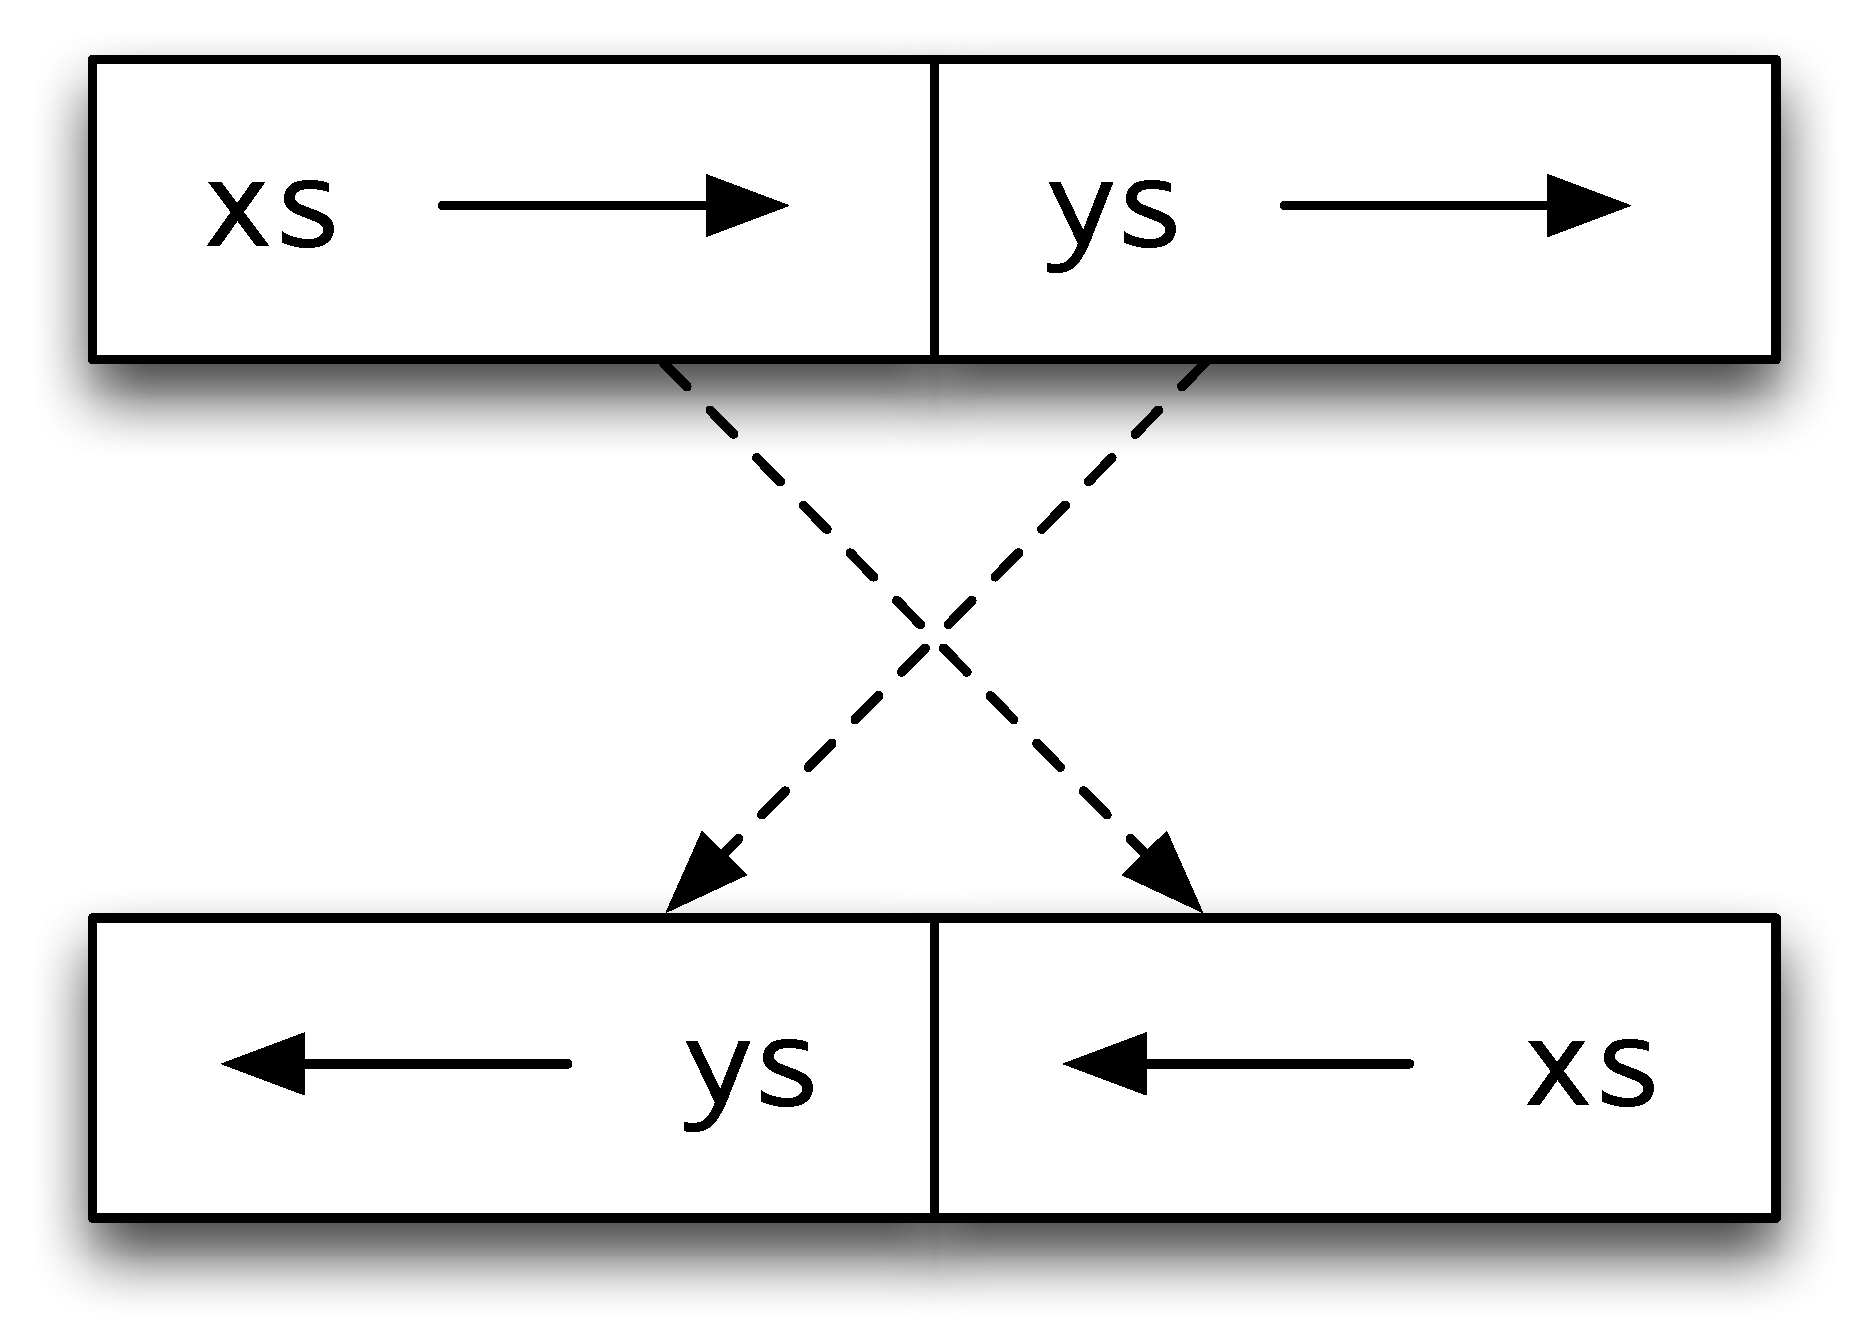
\includegraphics[width=2.5in]{Pictures/reverseSwap.pdf}
\end{center}
\caption{Reversing the list \texttt{xs++ys}}
\label{reverseSwap}
\end{figure}


\subsubexample*{2. \texttt{reverse} and \texttt{++}}\minx{reverse}\minx{++}

What happens when we reverse the join of two lists, \texttt{xs++ys}? The process is illustrated in Figure{reverseSwap}.
Each list is reversed, and they are swapped. In formal terms, 
\begin{alltt}
reverse (xs ++ ys) = reverse ys ++ reverse xs\hfill(reverse++)
\end{alltt}
where we define
\begin{alltt}
reverse []     = []\hfill(reverse.1)
reverse (z:zs) = reverse zs ++ [z]\hfill(reverse.2)
\end{alltt}
We will try to prove \texttt{(reverse++)} for all finite lists
\texttt{xs} and \texttt{ys}
by induction over \texttt{xs}.

\subparagraph*{Statement} The base case is
\begin{alltt}
reverse ([] ++ ys) = reverse ys ++ reverse []\hfill(base)
\end{alltt} 
and the induction goal is 
\begin{alltt}
reverse ((x:xs) ++ ys) = reverse ys ++ reverse (x:xs)\hfill(ind)
\end{alltt}
which is to be proved using the assumption
\begin{alltt}
reverse (xs ++ ys) = reverse ys ++ reverse xs\hfill(hyp)
\end{alltt}

\subparagraph*{Base} Simplifying both sides of \texttt{(base)} gives us 
\begin{alltt}
reverse ([] ++ ys) 
  = reverse ys \hfill \textrm{by }(++.1)

reverse ys ++ reverse []
  = reverse ys ++ [] \hfill \textrm{by }(reverse.1)
\end{alltt}
but we can prove the two equal only if we can show that appending an empty
list to the end of a list is an \textbf{identity} operation, that
is\index{identity}
\begin{alltt}
xs ++ [] = xs\hfill(++.3)
\end{alltt}
We leave a proof of this by induction over \texttt{xs} as an exercise for the reader.

\subparagraph*{Induction} Again, we look at the two sides of the equation, left-hand
side first.
\begin{alltt}
reverse ((x:xs) ++ ys) 
  = reverse (x:(xs ++ ys)) \hfill \textrm{by }(++.2)
  = reverse (xs ++ ys) ++ [x]  \hfill \textrm{by }(reverse.2)
  = (reverse ys ++ reverse xs) ++ [x]  \hfill \textrm{by }(hyp)
\end{alltt}
Examining the right-hand side, we have
\begin{alltt}
reverse ys ++ reverse (x:xs)
  = reverse ys ++ (reverse xs ++ [x]) \hfill \textrm{by }(reverse.2)
\end{alltt}
Now, these two are {\em almost\/} equal, except that the joins are
bracketed differently. We need another general property of \texttt{++},
namely that it is \textbf{associative}:
\begin{alltt}
xs ++ (ys ++ zs) = (xs ++ ys) ++ zs\hfill(++.4)
\end{alltt}
the proof of which we again leave as an exercise.\blackbox
\end{example}

\noindent This proof is instructive: it shows that often in proofs we use other
theorems or lemmas (the mathematician's term for a `little theorem') on
the way. If we do any serious proof we will build up a library of these
lemmas, with \texttt{(++.3)} and \texttt{(++.4)} being basic results about
\texttt{++} which we will call upon almost without thinking. We would expect
this library to resemble the standard prelude: it would contain all those
theorems which link the prelude functions and which will be called into use
whenever we use prelude functions. Many of the exercises at the end of the
section ask you to prove theorems concerning prelude functions.

\begin{figure}[t]\index{QuickCheck!properties over \texttt{[a]}}
\beware{QuickCheck and properties over \texttt{[a]}}{
If we test the QuickCheck property
\begin{alltt}
prop\_reversePlusPlus :: Eq a => [a] -> [a] -> Bool\\
\ \\
prop\_reversePlusPlus xs ys =\\
\hspace*{0.8cm}reverse (xs ++ ys) == reverse ys ++ reverse xs
\end{alltt}
we find that it holds. Fine, but if we check this property:
\begin{alltt}
prop\_reversePlusPlusOops :: Eq a => [a] -> [a] -> Bool\\
\ \\
prop\_reversePlusPlusOops xs ys =\\
\hspace*{0.8cm}reverse (xs ++ ys) == reverse xs ++ reverse ys
\end{alltt}
we find that this holds too! 

\medskip
What is happening here? The problem is that when we check a generic property -- that is one over a polymorphic type -- then it is in fact checked over a default type. This default type is \texttt{()}, which has exactly one element, also \texttt{()}. The incorrect property \emph{is} correct over lists of that type, because all their elements are the same!

\medskip
In order to restore sanity, it is enough to change the properties to a suitable non-generic type, using a type declaration like this:
\begin{alltt}
prop\_reversePlusPlusOops :: [Integer] -> [Integer] -> Bool
\end{alltt}
}
\end{figure}


\begin{exercises}

\item
Prove the properties for functions over \texttt{Picture} first discussed in Section \ref{proof}, that is, for all finite \texttt{pic}:
\begin{alltt}
flipV (flipH pic) = flipH (flipV pic)
flipV (flipV pic) = pic
flipH (flipV pic) = pic
\end{alltt}


\item
Look again at the properties for functions over \texttt{Picture} discussed in Section \ref{picturesAgain}, and prove those properties which should hold for all pictures.




\item
Prove for all finite \texttt{xs} and \texttt{ys} that
\begin{alltt}
sum (xs ++ ys) = sum xs + sum ys	\hfill(sum++)
\end{alltt}

\item
Prove the two rules for \texttt{++}:
\begin{alltt}
xs ++ [] = xs\hfill(++.3)
xs ++ (ys ++ zs) = (xs ++ ys) ++ zs\hfill(++.4)
\end{alltt}
for all finite \texttt{xs}, \texttt{ys} and \texttt{zs}.

\item
Show for all finite \texttt{xs} that
\begin{alltt}
sum (reverse xs)    = sum xs
length (reverse xs) = length xs
\end{alltt}
What common factors can you see in your two proofs?

\item
Show for all finite integer lists \texttt{xs} and \texttt{ys} that
\begin{alltt}
elem z (xs ++ ys) = elem z xs || elem z ys
\end{alltt}

\item
Show for all finite lists \texttt{ps} that
\begin{alltt}
zip (fst (unzip ps)) (snd (unzip ps)) = ps
\end{alltt}
Under what conditions on \texttt{xs} and \texttt{ys} is it the case that
\begin{alltt}
unzip (zip xs ys) = (xs,ys)
\end{alltt}
when \texttt{unzip} is defined by
\begin{alltt}\minx{unzip}
unzip [] = ([],[])
unzip ((x,y):ps) 
  = (x:xs,y:ys)
    where
    (xs,ys) = unzip ps                   
\end{alltt}
Give a proof in that case.

\item
\mbox{[Harder]} Show for all finite \texttt{xs} and defined \texttt{n} that
\begin{alltt}
take n xs ++ drop n xs = xs
\end{alltt}


\item
Write QuickCheck properties for the propositions that you have proved, and check that they indeed hold.

\end{exercises}
\index{induction|)}


\section{Generalizing the proof goal}
\label{genPrf}
\index{induction!generalizing the goal}

It is not always easy to build a proof in a straightforward way, by induction
over a goal we set ourselves. In this section we explore an example in which
we are able to build a proof of the property we
seek only after two false starts. 
The section is more challenging than the rest of the chapter and can safely
be omitted on first reading.


\subsection*{The shunting function}

The \texttt{shunt} function moves the elements from one list onto another, like this
\begin{alltt}
shunt :: [a] -> [a] -> [a]\minx{shunt}
\bl
shunt []     ys = ys\hfill (shunt.1)
shunt (x:xs) ys = shunt xs (x:ys) \hfill (shunt.2)
\end{alltt}
Starting with an empty second argument, we have
\begin{alltt}
shunt [2,3,1] []
\step shunt [3,1] [2]
\step shunt [1] [3,2]
\step shunt [] [1,3,2]
\step [1,3,2]
\end{alltt}
and so we can reverse lists using this function:
\begin{alltt}
rev :: [a] -> [a]\minx{rev}
rev xs = shunt xs []\hfill (rev.1)
\end{alltt}
Now we turn to looking at properties of the \texttt{rev} function.

\subsection*{First proof attempt}

Reversing a list twice should give us back the list we started with, and so
we aim to prove that 
\begin{alltt}
rev (rev xs) = xs \hfill Q(xs)
\end{alltt}
for
all finite lists \texttt{xs}. The base case is easily established, but when we
look at the induction step, we meet our first problem:
\begin{alltt}
rev (rev (x:xs))
  = shunt (shunt (x:xs) []) [] \hfill {\rm by} (rev.1)
  = shunt (shunt xs [x]) []\hfill {\rm by} (shunt.2)
\end{alltt} 
This has no direct relationship to the induction
hypothesis, which mentions only the function \texttt{rev}. A clue to the problem
is that \texttt{rev} is not the function defined by recursion --- it is simply a
specialization of \texttt{shunt}. Can we find a {\em generalization\/} of 
\texttt{Q(xs)} which talks explicitly about \texttt{shunt} and which is to be proved by
induction? 

In general the effect of \texttt{shunt xs ys} is to give
\begin{alltt}
(reverse xs) ++ ys
\end{alltt}
If we reverse this list, we should get
\begin{alltt}
(reverse ys) ++ xs
\end{alltt}
(try some examples!) and so we should be able to prove that
\begin{alltt}
shunt (shunt xs ys) [] = shunt ys xs
\end{alltt}
When \texttt{ys} is replaced by 
\texttt{[]}, we get \texttt{Q(xs)}. We therefore aim to prove this generalization.

\subsection*{Second proof attempt}

Our aim is to show
\begin{alltt}
shunt (shunt xs ys) [] = shunt ys xs
\end{alltt}
for all finite lists \texttt{xs} and \texttt{ys}. In the case that \texttt{xs} is {\mi
[]}, the proof is simple. Now we look at the induction step:
\begin{alltt}
shunt (shunt (x:xs) ys) [] 
  = shunt (shunt xs (x:ys)) [] \hfill {\rm by} (shunt.2)
\end{alltt}
We would now like to claim by induction that this is equal to \texttt{shunt
(x:ys) xs}, but to do this we need the induction hypothesis to give the result
that
\begin{alltt}
shunt (shunt xs (x:ys)) [] = shunt (x:ys) xs
\end{alltt}
rather than 
\begin{alltt}
shunt (shunt xs ys) [] = shunt ys xs\end{alltt}
To get around this, we strengthen the induction hypothesis to become
\begin{alltt}
shunt (shunt xs zs) [] = shunt zs xs {\rm for all finite lists} zs\end{alltt}
so that in particular it will hold when \texttt{(x:ys)} replaces \texttt{zs}. We now
try again.

\subsection*{The successful proof attempt} 

In logical notation, our goal is to prove
\begin{alltt}
\all{}zs (shunt (shunt xs zs) [] = shunt zs xs)
\end{alltt}
\index{\forall@$\forall$}
for all finite \texttt{xs} by induction.

\subparagraph*{Statement} Now we can state what is required. The base case is
\begin{alltt}
\all{}zs (shunt (shunt [] zs) [] = shunt zs []) \hfill (base)
\end{alltt}
and the induction step is to prove
\begin{alltt}
\all{}zs (shunt (shunt (x:xs) zs) [] = shunt zs (x:xs)) \hfill (ind)
\end{alltt}
assuming the induction hypothesis
\begin{alltt}
\all{}zs (shunt (shunt xs zs) [] = shunt zs xs) \hfill (hyp)
\end{alltt}

\subparagraph*{Base} In the base case we prove 
\begin{alltt}
\all{}zs (shunt (shunt [] zs) [] = shunt zs []) \hfill (base)
\end{alltt}
by proving it for an arbitrary \texttt{zs}. 
The left-hand side simplifies 
to the right-hand side in one step.
\begin{alltt}
shunt (shunt [] zs) []
  = shunt zs [] \hfill {\rm by} (shunt.1)
\end{alltt}

\subparagraph*{Induction} 
As in the base case, we prove  
\begin{alltt}
\all{}zs (shunt (shunt (x:xs) zs) [] = shunt zs (x:xs)) \hfill (ind)
\end{alltt}
by proving it for an arbitrary \texttt{zs}. Simplifying the left-hand side, we
have
\begin{alltt}
shunt (shunt (x:xs) zs) [] 
  = shunt (shunt xs (x:zs)) [] \hfill {\rm by} (shunt.2)
\end{alltt}
Now, by \texttt{(hyp)}, where we take the particular value \texttt{(x:zs)} to replace the
universally quantified variable \texttt{zs},
\begin{alltt}
  = shunt (x:zs) xs \hfill {\rm by} (hyp)
  = shunt zs (x:xs) \hfill {\rm by} (shunt.2)
\end{alltt}
This is the right-hand side, and so the proof is complete for an arbitrary
\texttt{ys}, giving a proof of \texttt{(ind)}, and completing the induction proof.
\blackbox

\medskip
\noindent
This example shows that we may have to generalize what has to be proved in
order for induction proofs to work. This seems paradoxical: we are making it
harder for ourselves, apparently. We are in one way, but at the same time we
make the induction hypothesis {\em stronger}, so that we have {\em more\/}
resources to use when proving the induction step.


\begin{exercises}
\item
Prove for all finite lists \texttt{xs} and \texttt{ys} that
\begin{alltt}
rev (xs ++ ys) = rev ys ++ rev xs
\end{alltt}

\item
Using the function
\begin{alltt}
facAux :: Integer -> Integer -> Integer
facAux 0 p = p
facAux n p = facAux (n-1) (n*p)
\end{alltt}
we can define
\begin{alltt}
fac2 n = facAux n 1
\end{alltt}
Prove that for all defined natural numbers \texttt{n},
\begin{alltt}
fac n = fac2 n
\end{alltt}


\item
Write a property expressing that the old and new \texttt{reverse} functions have the same behaviour.

\item
Write a property expressing that the old and new factorial functions have the same behaviour. What happens to the QuickCheck of the property if you allow arbitrary integer inputs to the factorial functions? how can you remedy this?




\end{exercises}


\begin{summary}
This chapter has shown that we can give Haskell programs a logical reading
which allows us to reason about them. Central to reasoning
about lists is the principle of structural induction, which does
for proof what primitive recursion does for definitions.

We gave a collection of hints about how we can build
proofs for functional programs, and illustrated these by giving a number of results
for common prelude functions such as \texttt{sum}, \texttt{++} and
\texttt{length}, as well as exercises involving others. We also saw how QuickCheck could be used to check whether or not a property appears to hold: this is a very useful way of making a `sanity check' of a property before we try to prove it.


\index{proof|)}

\end{summary}
%\end{document}

%\documentclass{book}\usepackage{sjtfonts}\usepackage{includegraphics}\usepackage{alltt}\usepackage{latexsym}
%\usepackage{array}
%\begin{document}\input{defs0}%		miradefs.tex 		    June 1994

% opening and closing a quoted Miranda section

\newcommand{\mira}{\noindent\hrulefill\nopagebreak\so}
\newcommand{\arim}{\nopagebreak\st\hrulefill\\}

% backslash in the Miranda environment
% Only feasible approach is to use \verb+\+
% in line!

%\newcommand{\bs}{$\mi\backslash\!\!$}
%\newcommand{\lbs}{\mbox{\verb+\+}}

% ignoring part of the input

\newcommand{\ignore}[1]{}

% a blank line in a Miranda section

\newcommand{\bl}{\mbox{\ }}

% Signalling a diffculty.

\definecolor{light-gray}{gray}{0.95}

\newcommand{\beware}[2]
 {\medskip\noindent\colorbox{light-gray}{\parbox{\textwidth}
 {\mbox{\large\textbf{#1}} \medskip\noindent\\ #2}\medskip\noindent}}

% Subscripting in Miranda text
\newcommand{\subscr}[2]{\mbox{${\mbox{\texttt{#1}}}_{\mbox{\texttt{#2}}}$}}

%\newcommand{\subscr}[2]{\mbox{${\mbox{\mi #1}}_{\mbox{\smtt #2}}$}}
\newcommand{\aone}{\subscr{a}{1}}
\newcommand{\atwo}{\subscr{a}{2}}
\newcommand{\ak}{\subscr{a}{k}}

\newcommand{\aoneone}{\subscr{a}{1,1}}

\newcommand{\eone}{\subscr{e}{1}}
\newcommand{\etwo}{\subscr{e}{2}}
\newcommand{\ei}{\subscr{e}{i}}
\newcommand{\er}{\subscr{e}{r}}

\newcommand{\fone}{\subscr{f}{1}}
\newcommand{\fl}{\subscr{f}{l}}

\newcommand{\gone}{\subscr{g}{1}}
\newcommand{\gtwo}{\subscr{g}{2}}
\newcommand{\gi}{\subscr{g}{i}}
\newcommand{\gr}{\subscr{g}{r}}

\newcommand{\hone}{\subscr{h}{1}}
\newcommand{\hl}{\subscr{h}{l}}

\newcommand{\pone}{\subscr{p}{1}}
\newcommand{\ptwo}{\subscr{p}{2}}
\newcommand{\pk}{\subscr{p}{k}}

\newcommand{\qone}{\subscr{q}{1}}
\newcommand{\qtwo}{\subscr{q}{2}}
\newcommand{\qk}{\subscr{q}{k}}

\newcommand{\rone}{\subscr{r}{1}}
\newcommand{\rtwo}{\subscr{r}{2}}

\newcommand{\tone}{\subscr{t}{1}}
\newcommand{\ttwo}{\subscr{t}{2}}
\newcommand{\tn}{\subscr{t}{n}}

\newcommand{\vone}{\subscr{v}{1}}
\newcommand{\vtwo}{\subscr{v}{2}}
\newcommand{\vn}{\subscr{v}{n}}

% for regular expressions

\newcommand{\stone}{\subscr{st}{1}}
\newcommand{\sttwo}{\subscr{st}{2}}
\newcommand{\stn}{\subscr{st}{n}}
\newcommand{\rthree}{\subscr{r}{3}}

\newcommand{\eps}{$\varepsilon$}
\newcommand{\trans}[1]{\stackrel{\mbox{\tt #1}}{\longrightarrow}}



% superscript in Miranda text

\newcommand{\superscr}[2]{\mbox{${\mbox{\mi #1}}^{\mbox{\smtt #2}}$}}

% Not equals in Miranda text

\newcommand{\noteq}{\makebox[0pt][l]{=}/}
\newcommand{\overslash}{\makebox[0pt][l]{/}}

% Definitions in complexity chapter

\newfont{\oldSym}{cmsy10}
\newcommand{\Th}{\boldmath$\oldSym\Theta$}
\newcommand{\pow}[1]{\^{}#1}
\newcommand{\leqq}{$\leq$}
\newcommand{\geqq}{$\geq$}
\newcommand{\lll}{$\ll$}
\newcommand{\eqq}{$\equiv$}
\newcommand{\ltwo}{\subscr{log}{2}}

% Indexing

\newcommand{\minx}[1]{\index{#1@{\ttfamily{}#1}}}
\setcounter{chapter}{8}\setcounter{page}{143}

\chapter{Generalization: patterns of computation}
\chapstart
\label{patternsGen}

Software reuse is a major goal of the software industry.
One of the great strengths of modern functional programming languages
like Haskell is that we can use them to define
general functions which can be used in many different applications. The Haskell
prelude functions over lists, for instance, 
form a toolkit to which we turn again and again in a host of
situations.

We have already seen one aspect of
this generality in \textbf{polymorphism}, under which the same program can
be used over many different types. The 
prelude functions over lists introduced in Chapter \ref{tupleList} 
provide many examples of this
including \texttt{length}, \texttt{++} and \texttt{take}. 

As we said, these functions have the same effect over every argument --
\texttt{length} computes the length of a list of any type, for instance. In this
chapter we explore a second mechanism, by which we can write functions
which embody a \textbf{pattern of computation}; two examples of what we mean 
\index{pattern of computation}
follow. 
\begin{itemize}
\item {\em Transform every element of a list in some way}. We might turn every
alphabetic character into upper case, or double every number.
\item {\em Combine the elements of a list using some operator}. We could add
together the elements of a numeric list in this way, for example.
\end{itemize}
How can we write general functions which implement patterns like this? 
We need to make the transformation
or operator into a \textbf{parameter} of the general function; in other
words we need to have functions as arguments of other functions. These 
\textbf{higher-order functions} are
the topic of this chapter.
Complementing this is the ability to make functions the \textbf{results}
of functions; we look at that in the next chapter.

We begin the chapter by examining the patterns of computation
over lists which we have encountered so far, and in the remaining
sections of the chapter we show how these are realized as higher-order
Haskell functions. We also re-examine primitive recursive definitions,
and see that they generalize the process of combining the elements of a
list using an operator. 

Next we look at an example of generalization: taking a
function over \texttt{String} into a polymorphic, higher-order function.
We do this by identifying the parts of the function which make it
specific to
\texttt{String} and turning those into a parameter of the function.
The example serves as a model for how we can generalize functions in any situation and so make them applicable in many more contexts. 


We conclude by revisiting a number of the case studies we have looked at earlier, and encourage you to look at these again, bearing in mind the new patterns of computation introduced in this chapter.

\section{Patterns of computation over lists}
\label{defForms}
\index{pattern of computation!over lists|(}

Many of the definitions of list processing functions we have seen so far
fall into a small number
of different sorts. In this section we look back over the previous chapters and discuss
the patterns which emerge. These patterns are realized as Haskell functions
later in the chapter.

\subsection*{Applying to all -- mapping}
\index{mapping}

Many functions call for all of the elements of a list to be transformed in some
way -- this we call {\bf mapping}. We have seen examples of this from the first chapter, where
we noted that to flip a picture in a vertical mirror -- \texttt{flipV} -- 
we needed to \texttt{reverse} each line of the \texttt{Picture}, which is a list of lines. 

We also saw mapping in
Chapter \ref{tupleList} in our first example of a list comprehension 
which was to double every element of a list of integers. 
\begin{alltt}
doubleAll [2,3,71] = [4,6,142]\minx{doubleAll}
\end{alltt}
Other
examples include
\begin{titemize}
\item taking the second element of each pair in  a list of pairs, as we do in the library
database;
\item in the supermarket billing example, converting every item in a list of bar codes to the corresponding 
\texttt{(Name,Price)} pair;
\item formatting each \texttt{(Name,Price)} pair in a list.
\end{titemize}

\subsection*{Selecting elements -- filtering}
\index{filter}

Selecting all the elements of a list with a given property is also common.
Chapter \ref{tupleList} contains the example of the function which selects the
digits from a string
\begin{alltt}
digits "29 February 2004" = "292004"\minx{digits}
\end{alltt}
Among the other cases we have seen are
\begin{titemize}
\item select each pair which has a particular person as its first element;
\item select each pair which is {\em not\/} equal to the loan pair being
returned.
\end{titemize}

\subsection*{Combining the items -- folding}
\index{folding}

The first example of primitive recursion in Chapter \ref{defFunLists} was
\texttt{sum}, 
\minx{sum}
which computes the total
of a list of integers. The total of the list is given by 
\textbf{folding} the function \texttt{+} into the list, thus:
\begin{alltt}
sum [2,3,71] = 2+3+71
\end{alltt}
In a similar way, 
\begin{titemize}
\item\ \texttt{++} can be folded into a list of lists to concatenate
it, as is done in the definition of \texttt{concat};
\minx{concat}\minx{++}
\item\ \texttt{\&\&} can be folded into a list of Booleans to take their
conjunction: this is the prelude function \texttt{and}; 
\item\ \texttt{max} can be folded into a list of integers to give their maximum.
\end{titemize}

\subsection*{Breaking up lists}

A common pattern in the text processing example of Chapter \ref{defFunLists} 
is to take or drop items from a list while they have some property. 
A first example is
\texttt{getWord},
\begin{alltt}
getWord "cat dog" = "cat"\minx{getWord}
\end{alltt}
in which we continue to take characters while they are alphabetic.
Other examples include \texttt{dropWord}, \texttt{dropSpace} and
\texttt{getLine}. In the last of these
the property in question depends not only upon the particular list item but also on
the part of the list selected so far.

\subsection*{Combinations}

These patterns of definition are often used together. In defining 
\texttt{books} for the library database, which returns all the books on loan to a
given person, we filter out all pairs involving the person, and then take all
second components of the results. The strength of list comprehensions is that
they give this combination of mapping and filtering,\index{list comprehensions}
which fits some examples -- like the library database -- particularly well.

Other combinations of functions are also common.
\begin{titemize}
\item In the pictures case study the function \texttt{invertColour}\minx{invertColour} 
inverts the colour of every character in a \texttt{Picture} 
by inverting every line; inverting a line requires us to invert every character, 
so here we have two, 
nested, uses of mapping.
\item Formatting the item part of a supermarket bill involves processing each
item in some way, then combining the results, using \texttt{++}.
\end{titemize}

\subsection*{Primitive recursion and folding}
\index{folding!and primitive recursion}
\index{primitive recursion!and folding}

The form of many definitions is primitive recursive. Sorting by
insertion is a classic example:\index{sorting!insertion}
\begin{alltt}
iSort []     = []\minx{iSort}
iSort (x:xs) = ins x (iSort xs)
\end{alltt}
Haskell provides a mechanism to turn a prefix function\index{function!prefix} like \texttt{ins}
into an infix\index{function!infix}
version. The name is enclosed by back quotes, \texttt{`ins`}, so
\begin{alltt}
iSort (x:xs) = x `ins` (iSort xs)
\end{alltt}
and, in a given example, we have
\begin{alltt}
iSort [4,2,3] = 4 `ins` 2 `ins` 3 `ins` []
\end{alltt}
Looked at this way, the definition looks like \texttt{`ins`} folded into the
list \texttt{[4,2,3]}. We shall look at this again in Section \ref{foldPrimRec}. 

\subsection*{The last 10\%}

The different kinds of definition discussed so far have all been primitive
recursive: we were able to define the result for \texttt{(x:xs)} in terms of the
result for \texttt{xs}. It has been said that at least 90\% of all definitions of
list processing functions are primitive recursive. Some are not, however; in
Chapter \ref{defFunLists} notable examples are quicksort and the \texttt{splitLines}
function,
\begin{alltt}\minx{splitLines}
splitLines [] = []
splitLines ws
  = getLine lineLen ws
         : splitLines (dropLine lineLen ws)
\end{alltt}
For a non-empty list of words \texttt{ws}, the result \texttt{splitLines ws} is defined using
a recursive call of \texttt{splitLines} not on the tail of \texttt{ws} but on 
\texttt{(dropLine lineLen ws)}.
This form of recursion will terminate
because \texttt{(dropLine lineLen ws)} will always be shorter than \texttt{ws} itself,
at least in sensible cases where no word in the list \texttt{ws} is longer than the line
length \texttt{lineLen}.  

\index{pattern of computation!over lists|)}


\section{Higher-order functions: functions as arguments}
\label{hofs}
\index{function!higher-order}
\index{higher-order function}

A function is \textbf{higher-order} if it takes a function as an
argument or returns a function as a result, or does both. In this section we
show how a variety of functions, including some of the patterns
discussed in the last section, can be written using functions as
arguments.

\subsection*{Mapping -- the \texttt{map} function}

We can double all the elements in an integer list in two ways, either
using a list comprehension,
\begin{alltt}\minx{doubleAll}
doubleAll :: [Integer] -> [Integer]
doubleAll xs = [ 2*x | x <- xs ]
\end{alltt}
or using primitive recursion,
\begin{alltt}
doubleAll []     = []
doubleAll (x:xs) = 2*x : doubleAll xs
\end{alltt}
In both cases, we can see that the specific operation of multiplying
by two is applied to an element of the list in the expression `\texttt{2*x}'. 

Suppose that we want to modify every element of
a list by
another operation -- for instance, the function \texttt{ord} that transforms 
a \texttt{Char} into an \texttt{Int} --
we could modify one of the definitions above by replacing the `\texttt{2*x}' 
by `\texttt{fromEnum x}' to give a different definition. 

Taking this approach would mean that we would write a whole lot of
definitions which differ only in the function used to make the
transformation. Instead of doing this, we can write a {\em single\/}
definition in which the 
function becomes a \textbf{parameter} of the
definition. Our general definition will be
\begin{alltt}\index{map@\texttt{map}}
map f xs = [ f x | x <- xs ]\hfill(map.0)
\end{alltt}
or we can give an explicit primitive recursion
\begin{alltt}
map f []     = []\hfill(map.1)
map f (x:xs) = f x : map f xs\hfill(map.2)
\end{alltt}
The function to \texttt{double} all the elements of a list can now be given
by applying \texttt{map} to two things: the transformation -- \texttt{double} -- and
the list in question.
\begin{alltt}
doubleAll xs = map double xs	       
\end{alltt}
where \texttt{double x = 2*x}. In a similar way, 
the function to convert all the characters into their codes will be
\begin{alltt}\minx{convertChrs}
convertChrs :: [Char] -> [Int]
convertChrs xs = map fromEnum xs
\end{alltt}
In the \texttt{Picture} case study to flip a picture in a vertical
mirror we can write
\begin{alltt}\minx{flipV}
flipV :: Picture -> Picture
flipV xs = map reverse xs
\end{alltt}
What is the type of \texttt{map}? It takes two arguments -- the first is
a function, 
and
the second is a list -- and it returns a list. 
\begin{center}
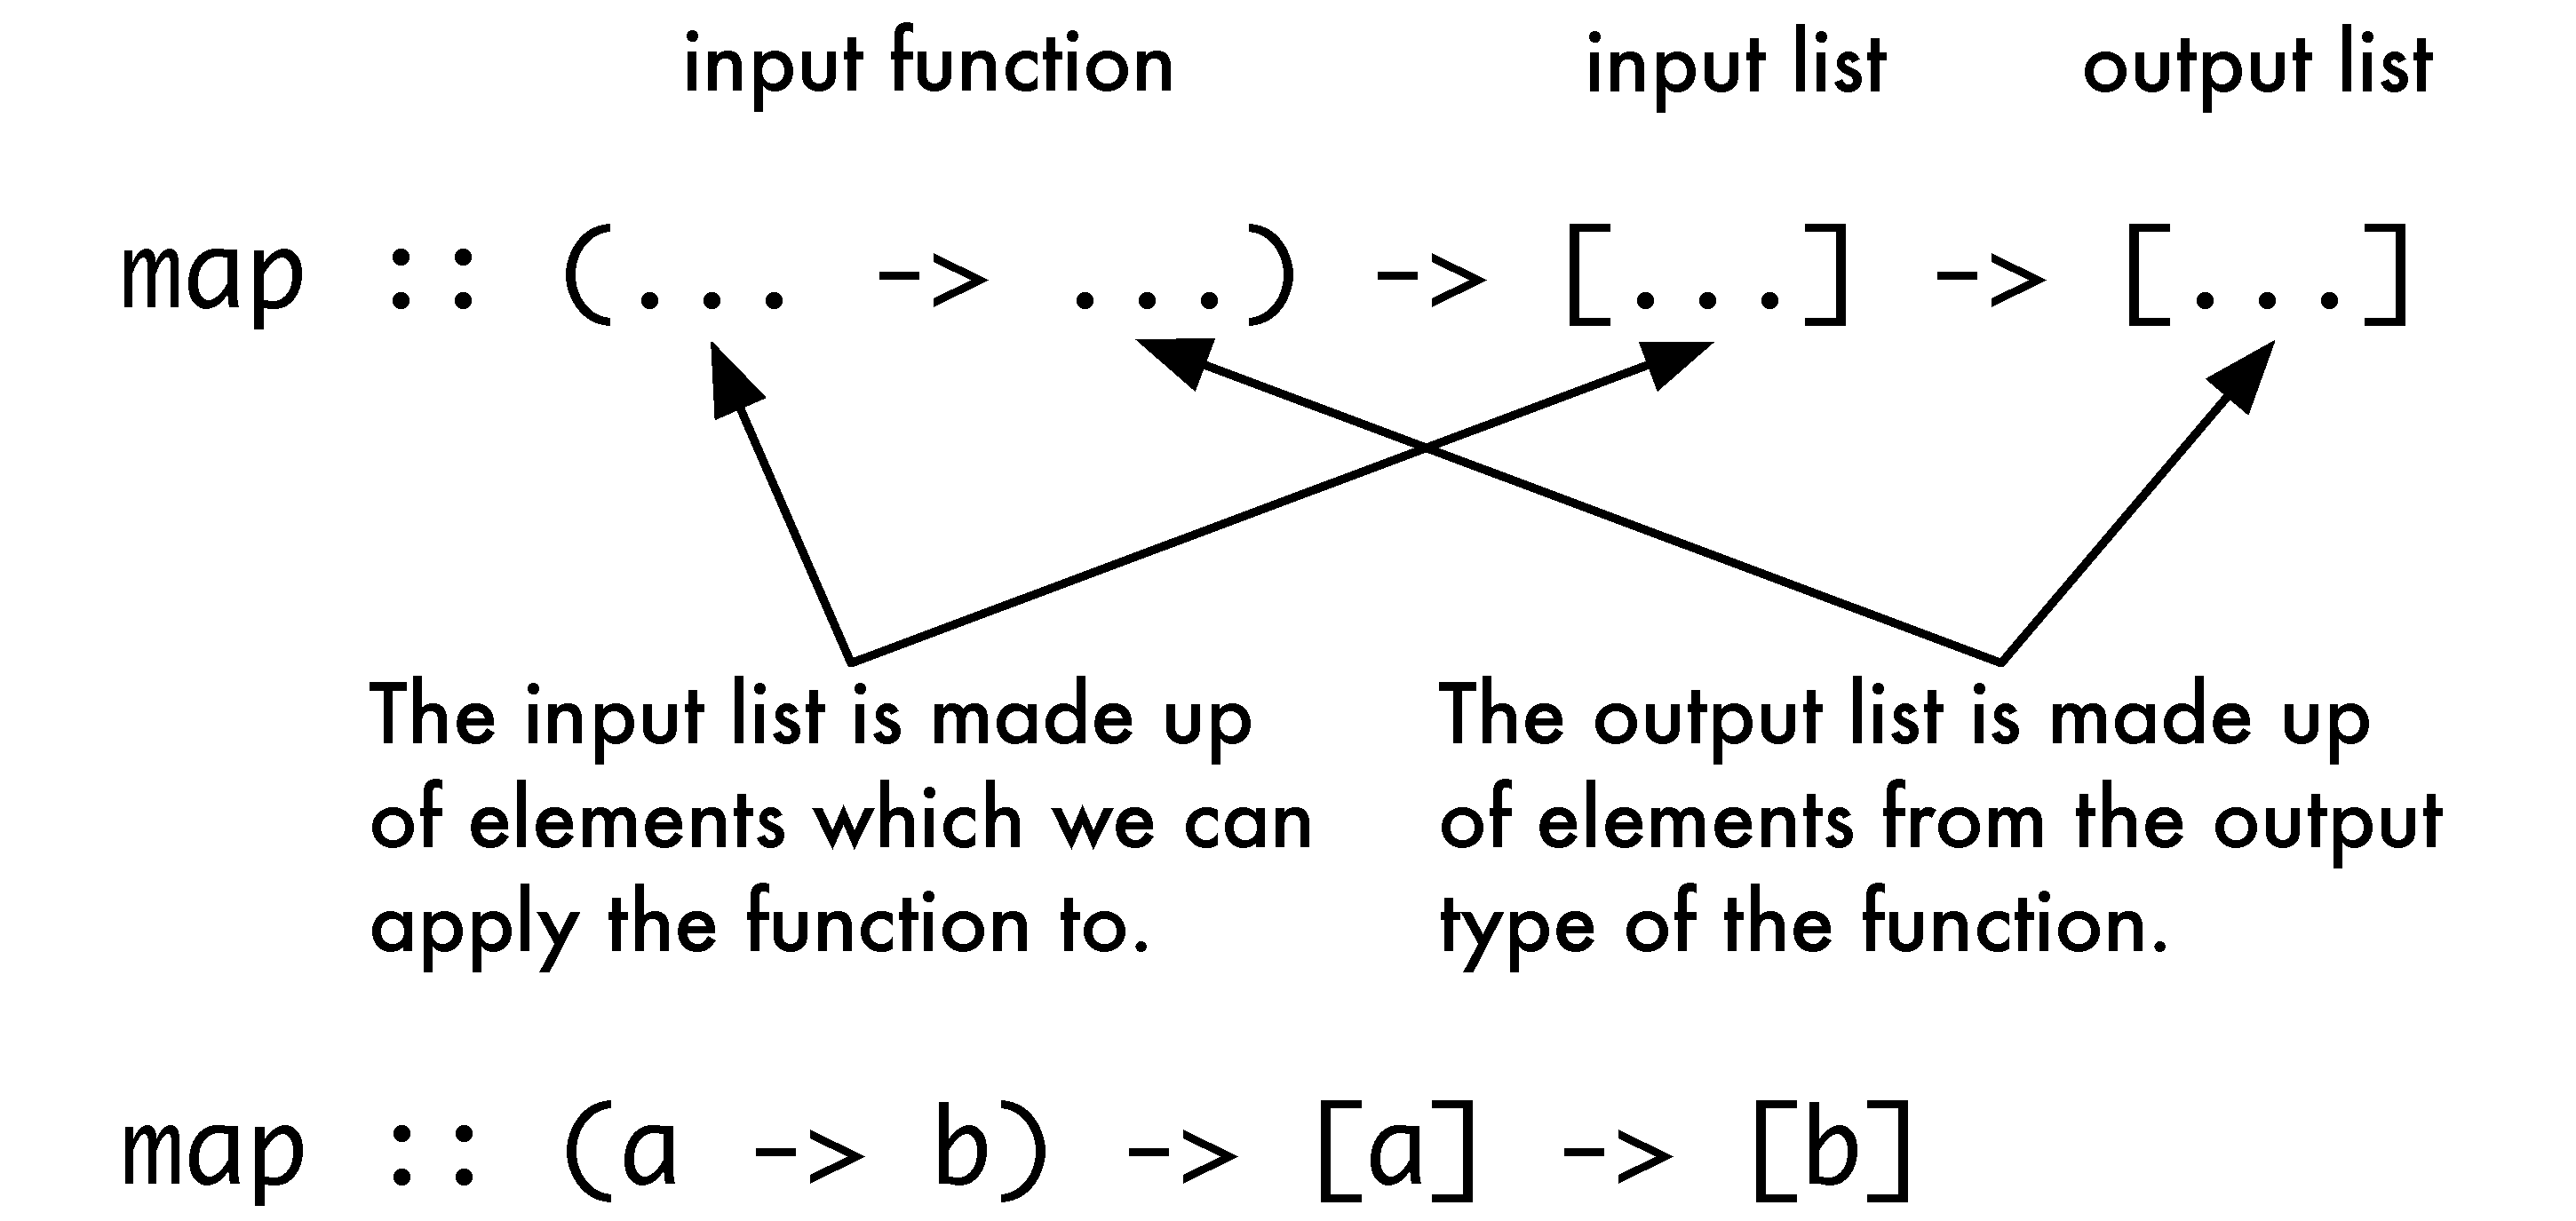
\includegraphics[width=4in]{Pictures/mapType.pdf}
\end{center}
The 
figure shows how the types of the functions and lists are related,
giving \texttt{map} the type
\begin{alltt}\index{map@\texttt{map}!type of}
map :: (a -> b) -> [a] -> [b]
\end{alltt}
where recall that \texttt{a} and \texttt{b} are type variables, standing
for arbitrary types.
Instances of the type of \texttt{map} include
\begin{alltt}
map :: (Integer -> Integer) -> [Integer] -> [Integer]
\end{alltt}
as used in the definition of \texttt{doubleAll}, where \texttt{map} is applied to
the function \texttt{double} of type \texttt{Int -> Int} and
\begin{alltt}
map :: (Char -> Int) -> [Char] -> [Int]
\end{alltt}
as in the definition of \texttt{convertChrs}.

\subsection*{Modelling properties as functions}
\index{properties as functions}
\index{function!representing properties}

Before defining the function to \textbf{filter}, or  select, 
those elements of a list having a given property, we need to think about how such
properties are to be modelled in Haskell. Take the example of filtering
the digits from a string -- the function \texttt{digits}
mentioned earlier. How is the property of `being a digit' to be
modelled? We have already seen that the library \texttt{Data.Char} contains a function
\begin{alltt}\minx{isDigit}
isDigit :: Char -> Bool
\end{alltt}
and we find out whether a particular character like \texttt{'d'} is a
digit or not by applying the function to the character to give a
Boolean result, that is \texttt{True}
or \texttt{False}.

This is the way that we can model a \textbf{property}\index{property}
over any type \texttt{t}.
The property is given by a function of type
\begin{alltt}
t -> Bool 
\end{alltt}
and an element
\texttt{x} has the property precisely when \texttt{f x} has the value
\texttt{True}. We have already seen the example of \texttt{isDigit};
other examples include
\begin{alltt}\minx{isEven}\minx{isSorted}
isEven :: Integer -> Bool
isEven n = (n `mod` 2 == 0)

isSorted :: [Integer] -> Bool
isSorted xs = (xs == iSort xs)
\end{alltt}
We usually adopt the convention that the names of properties begin with `\texttt{is}'.
\index{conventions!names of properties}

\subsection*{Filtering -- the \texttt{filter} function}
\index{filter@\texttt{filter}}

Building on our discussion of properties, we see that the \texttt{filter}
function will take a property and a list, and return those elements of
the list having the property:
\begin{alltt}
filter p [] = []\hfill(filter.1)
filter p (x:xs)
  | p x         = x : filter p xs\hfill(filter.2)
  | otherwise   =     filter p xs\hfill(filter.3)
\end{alltt}
In the case of an empty list, the result is empty.
For a non-empty list
\texttt{(x:xs)} there are two cases. If the guard condition \texttt{p x} is
true then the element \texttt{x} is the first element of the result list; the remainder
of the result is given by selecting those elements in \texttt{xs} which have the property 
\texttt{p}. If \texttt{p x} is \texttt{False}, \texttt{x} is not included, and the result is
given by searching \texttt{xs} for elements with 
property \texttt{p}.

A list comprehension also serves to define \texttt{filter},
\begin{alltt}
filter p xs = [ x | x <- xs , p x ]\hfill(filter.0)
\end{alltt}
where again we see that the condition for inclusion of \texttt{x} in the list is
that it has the property \texttt{p}.

Our example \texttt{digits}
is defined using \texttt{filter} as follows
\begin{alltt}\minx{digits}
digits xs = filter isDigit xs
\end{alltt}
Other applications of \texttt{filter} give
\begin{alltt}
filter isEven [2,3,4,5]                    \step [2,4]
filter isSorted [[2,3,4,5],[3,2,5],[],[3]] \step [[2,3,4,5],[],[3]]
\end{alltt}

What is the type of \texttt{filter}? It takes a property and a list, and
returns a list.
\begin{center}\index{filter@\texttt{filter}!type of}
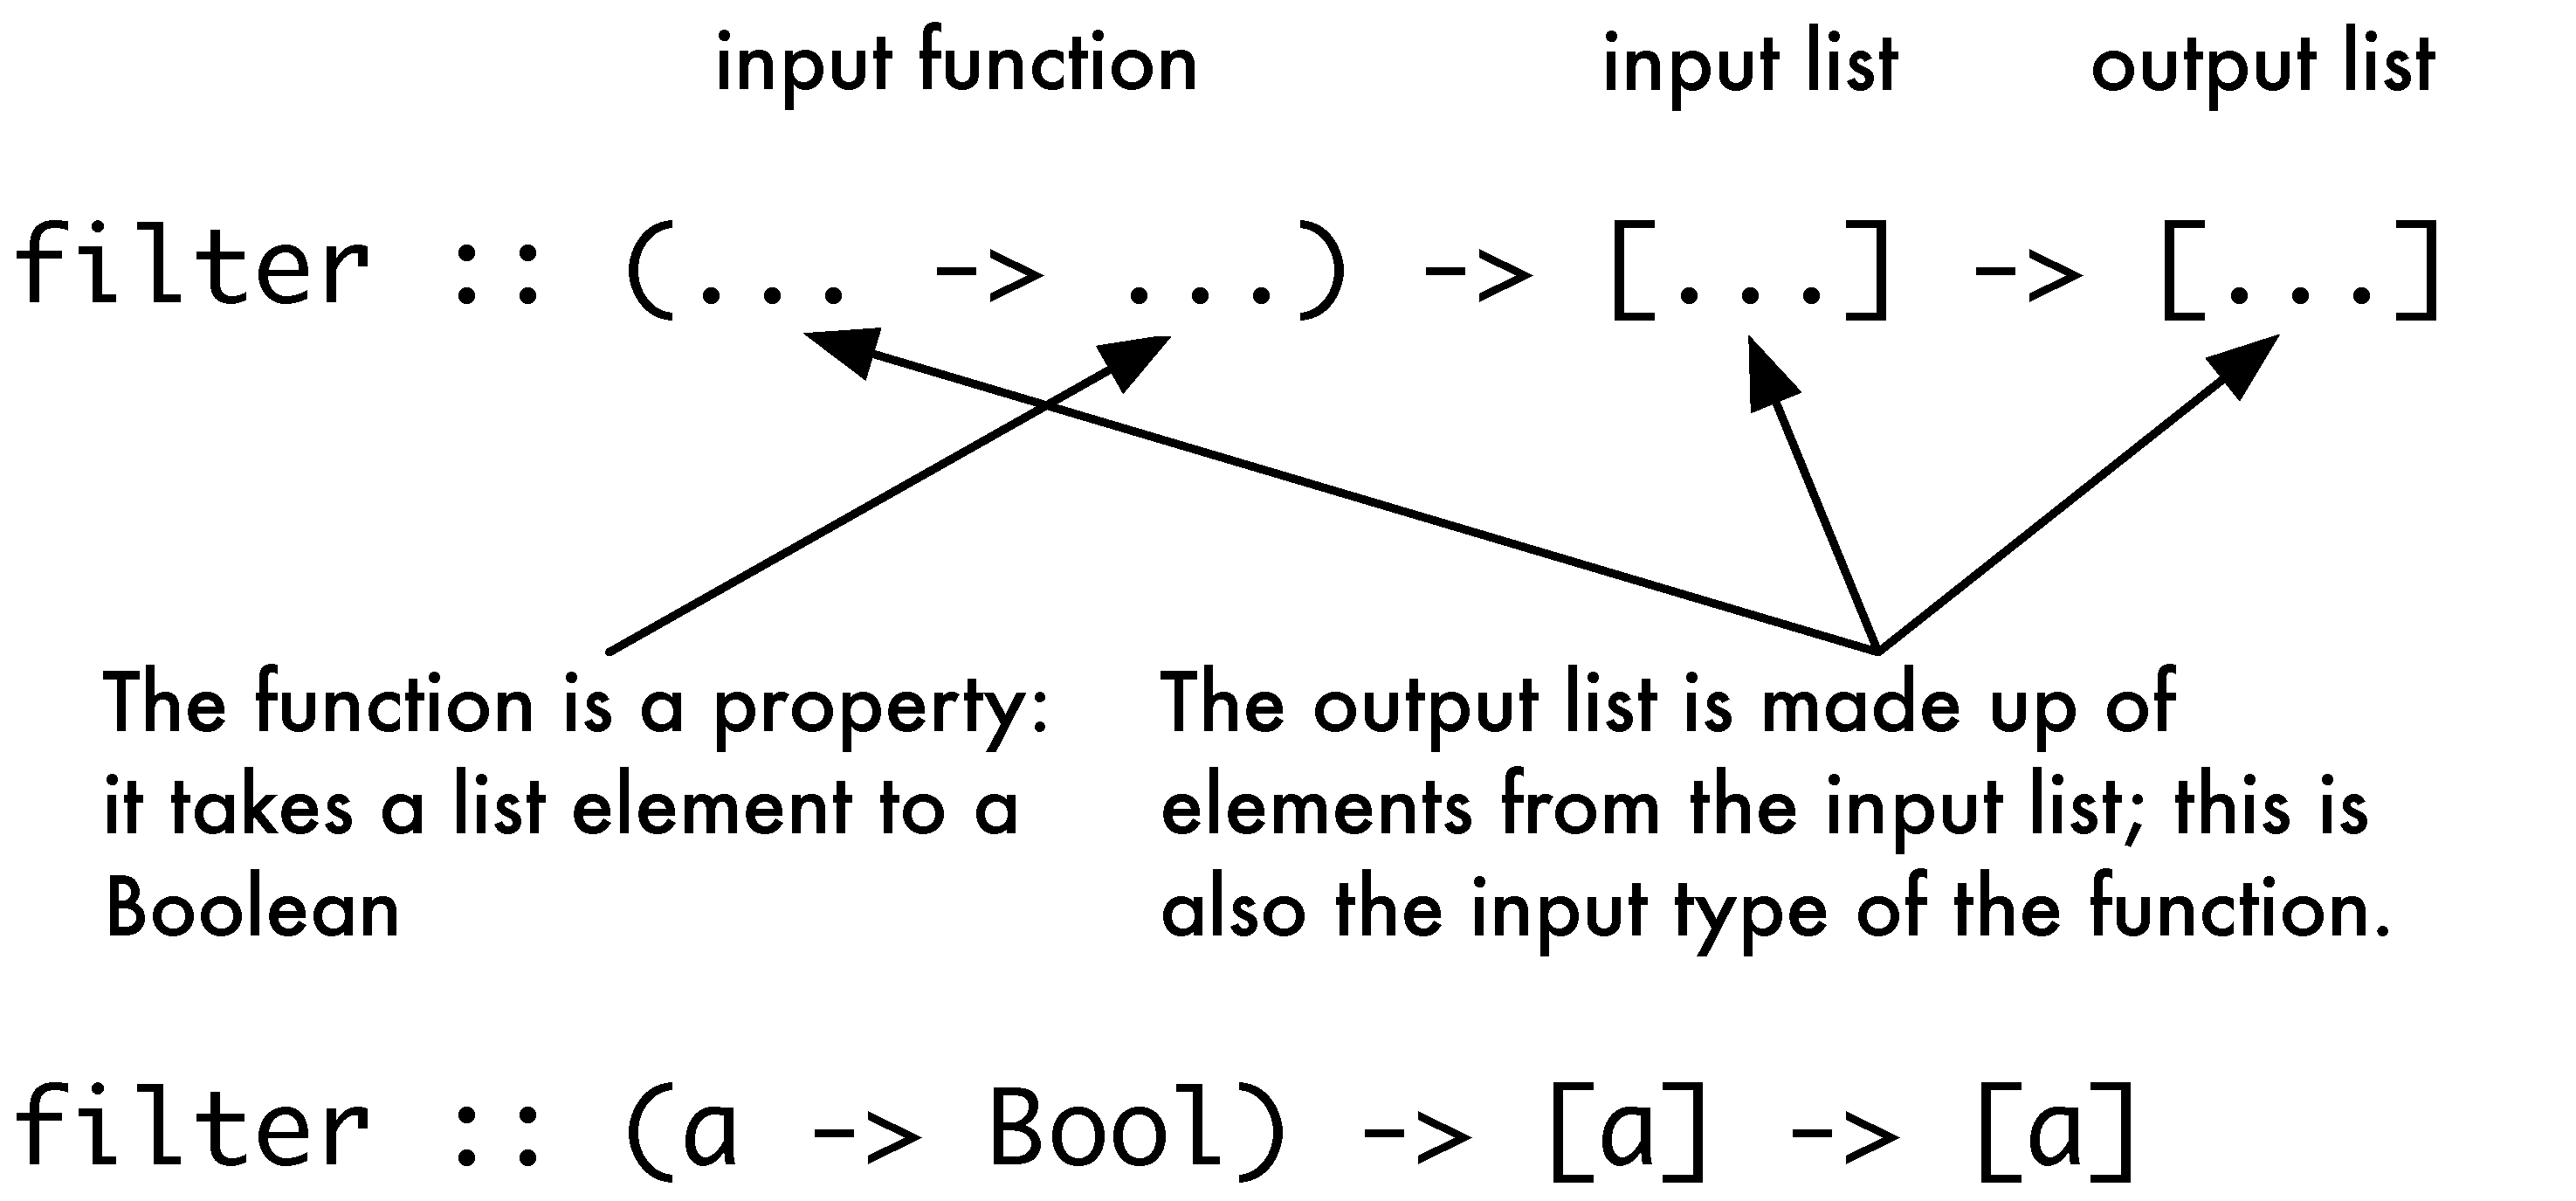
\includegraphics[width=4in]{Pictures/filterType.pdf}
\end{center}

\subsection*{Combining \texttt{zip} and \texttt{map} -- the
\texttt{zipWith} function}\index{zipWith@\texttt{zipWith}}

We have already seen the polymorphic function
\begin{alltt}
zip :: [a] -> [b] -> [(a,b)]
\end{alltt}
which `zips together' the the elements of two lists into a single list of pairs, pairing up corresponding elements in the two lists. For instance,
\begin{alltt}\index{Frank}
zip [2,3,4] "Frank" = [(2,'F'),(3,'r'),(4,'a')]
\end{alltt}
As the example shows, if the lists are of different lengths, we just drop the elements in the longer list with no element to pair with.

What happens if we want to do something to two corresponding elements 
other than making a
pair of them? Recall from Chapter \ref{intro} that in our \texttt{Picture}
case study to define \texttt{beside} we wanted to join
corresponding lines using (++).
To this end we define the \texttt{zipWith} function, which combines the
effect of zipping and mapping:
\begin{alltt}
zipWith f (x:xs) (y:ys) = f x y : zipWith f xs ys
zipWith f  _      _     = []
\end{alltt}
In the first case we see that if both lists are non-empty
we apply the function \texttt{f} to their heads to give the first element
of the result, and zip their tails with \texttt{f} in a similar way. In
the second case -- when at least one of the inputs is \texttt{[]} -- the
result is \texttt{[]}, just as it was in the definition of \texttt{zip}.

Returning to the \texttt{Picture} case study, we can then define
\begin{alltt}\minx{beside}
beside :: Picture -> Picture -> Picture
beside pic1 pic2 = zipWith (++) pic1 pic2
\end{alltt}
What is the type of \texttt{zipWith}?
The function takes three arguments. The second and third are lists of
arbitrary type, \texttt{[a]} and \texttt{[b]} respectively. The result is also
a list of arbitrary type, \texttt{[c]}. Now, the first argument is
applied to elements of the input lists to give an element of the output
list, so it must have type
\texttt{a -> b -> c}. Putting this together, we have
\begin{alltt}\index{zipWith@\texttt{zipWith}!type of}
zipWith :: (a -> b -> c) -> [a] -> [b] -> [c]
\end{alltt}

In the exercises we look further at the examples defined here, as well
as introducing other higher-order functions.

\begin{exercises}

\item
Write three line-by-line calculations of \texttt{doubleAll [2,1,7]} using
the three different definitions of \texttt{doubleAll} that use a list
comprehension, primitive recursion and \texttt{map}.

\item
How would you define the \texttt{length} function using \texttt{map} and
\texttt{sum}?


\item
Given the function
\begin{alltt}
addUp ns = filter greaterOne (map addOne ns)
\end{alltt}
where
\begin{alltt}
greaterOne n = n>1
addOne n     = n+1
\end{alltt}
how would you redefine it using \texttt{filter} before \texttt{map}, as
in
\begin{alltt} 
addUp ns = map fun1 (filter fun2 ns)
\end{alltt}

\item
Describe the effect of 
\begin{alltt}
map addOne (map addOne ns) 
\end{alltt}
Can you conclude anything in general about properties of
\texttt{map f (map g xs)}
where \texttt{f} and \texttt{g} are arbitrary functions?

\item
What is the effect of 
\begin{alltt}
filter greaterOne (filter lessTen ns)
\end{alltt}
where \texttt{lessTen n = n<10}? What about the general case of
\begin{alltt}
filter p (filter q xs)
\end{alltt}
where \texttt{p} and \texttt{q} are arbitrary properties?

\item
Give definitions of functions to take a list of integers, \texttt{ns}, and
\begin{titemize}
\item return the list consisting of the squares of the integers in \texttt{ns};
\item return the sum of squares of items in \texttt{ns};
\item check whether all items of the list are greater than zero.
\end{titemize}

\item
Using functions defined already wherever possible, write definitions of functions to 
\begin{titemize}
\item give the minimum value of a function \texttt{f} on inputs \texttt{0} to \texttt{n};
\item test whether the values of \texttt{f} on inputs \texttt{0} to \texttt{n} are all
equal;
\item test if all values of \texttt{f} on inputs \texttt{0} to \texttt{n} are greater
than zero, and,
\item check whether the values \texttt{f 0}, \texttt{f 1} to \texttt{f n} are in
increasing order.
\end{titemize}

\item
State the type of and define a function \texttt{twice} which takes a function from integers to integers
and an input integer, and whose output is the function applied to the input
twice. For instance, with the \texttt{double} function and \texttt{7} as input,
the result is \texttt{28}. What is the most general type of the function
you have defined?

\item
Give the type of and define a function \texttt{iter} so that
\begin{alltt}
iter n f x = f (f (f \ldots (f x)\ldots))  
\end{alltt}
where \texttt{f} occurs \texttt{n} times on the right-hand side of the equation.
For instance, we should have
\begin{alltt}
iter 3 f x = f (f (f x))
\end{alltt}
and \texttt{iter 0 f x} should return \texttt{x}.

\item
Using \texttt{iter} and \texttt{double} define a function which on input \texttt{n} 
returns $\texttt{2}^{\texttt{n}}$; remember that 
$\texttt{2}^{\texttt{n}}$ means one multiplied by two \texttt{n}
times.

\item
Define QuickCheck properties that you would expect to hold for the result of a \texttt{filter},
\begin{alltt}
filter p xs
\end{alltt}

\item
Suppose that \texttt{g} is the \emph{inverse} of \texttt{f}, so that 
\begin{alltt}
g (f x) \step{}x
f (g y) \step{}y
\end{alltt}
for all \texttt{x} and \texttt{y}, give properties that you would expect to hold for the result of the \texttt{map}:
\begin{alltt}
map f xs
\end{alltt}

\end{exercises}

\section{Folding and primitive recursion}
\label{foldPrimRec}
\index{folding!and primitive recursion|(}
\index{primitive recursion!and folding|(}


In this section we look at a particular sort of higher-order function
which implements the operation of \textbf{folding} an operator or function into a
list of values. We will see that this operation is more general than we
might first think, and that most primitive recursive functions over
lists can, in fact, be defined using a fold.

\subsection*{The functions \texttt{foldr1} and \texttt{foldr}}
\index{folding}
\index{foldr1@\texttt{foldr1}}\index{foldr@\texttt{foldr}}

Here we look at two sorts of folding function. First
we look at a function which folds a function into a non-empty list; it is defined in
\texttt{GHC.List} and is called \texttt{foldr1}; we will discuss why it is 
called this later in the section.

The definition of \texttt{foldr1}\index{foldr1@\texttt{foldr1}} will have two cases. 
Folding \texttt{f} into the singleton list \texttt{[a]} gives \texttt{a}.
Folding \texttt{f} into a longer list is given by 
\begin{alltt}
foldr1 f [\eone,\etwo,\ldots,\subscr{e}{k}]
  = \eone `f` (\etwo `f` ( \ldots `f` \subscr{e}{k})\ldots)
  = \eone `f` (foldr1 f [\etwo,\ldots,\subscr{e}{k}])
  = f \eone (foldr1 f [\etwo,\ldots,\subscr{e}{k}])
\end{alltt}
The Haskell definition is therefore
\begin{alltt}
foldr1 f [x]    = x\hfill(foldr1.1)
foldr1 f (x:xs) = f x (foldr1 f xs)\hfill(foldr1.2)
\end{alltt}
and the type of \texttt{foldr1} will be given by
\begin{alltt}\index{foldr1@\texttt{foldr1}!type of}
foldr1 :: (a -> a -> a) -> [a] -> a
\end{alltt}
The type shows that \texttt{foldr1} has two arguments.
\begin{itemize}
\item The first argument is a binary function over the type \texttt{a}; for
example, the function \texttt{(+)} over \texttt{Int}.
\item The second is a list of elements of type \texttt{a} which are to
be combined using the operator; for instance, \texttt{[3,98,1]}
\end{itemize}
The result is a single value of type \texttt{a}; in the running example we
have 
\begin{alltt}
foldr1 (+) [3,98,1] = 102
\end{alltt}
Other examples which use \texttt{foldr1} include
\begin{alltt}
foldr1 (||) [False,True,False] = True
foldr1 (++) ["Freak ", "Out" , "", "!"] = "Freak Out!"
foldr1 min [6] = 6
foldr1 (*) [1 ..\ 6] = 720
\end{alltt}
The function \texttt{foldr1} gives an error when applied to an empty list argument.

We can modify the
definition to give an extra argument which is the value returned on the empty list, so giving 
a function defined on all finite lists. This
function is called \texttt{foldr} 
and
is defined as follows
\begin{alltt}\index{foldr@\texttt{foldr}}
foldr f s []     = s\hfill(foldr.1)\index{foldr@\texttt{foldr}}
foldr f s (x:xs) = f x (foldr f s xs)\hfill(foldr.2)
\end{alltt}
The `\texttt{r}' in the definition is for `fold, bracketing to the \textbf{right}'.
Using this slightly more general function, whose type we predict is
\begin{center}\index{foldr@\texttt{foldr}!type of}
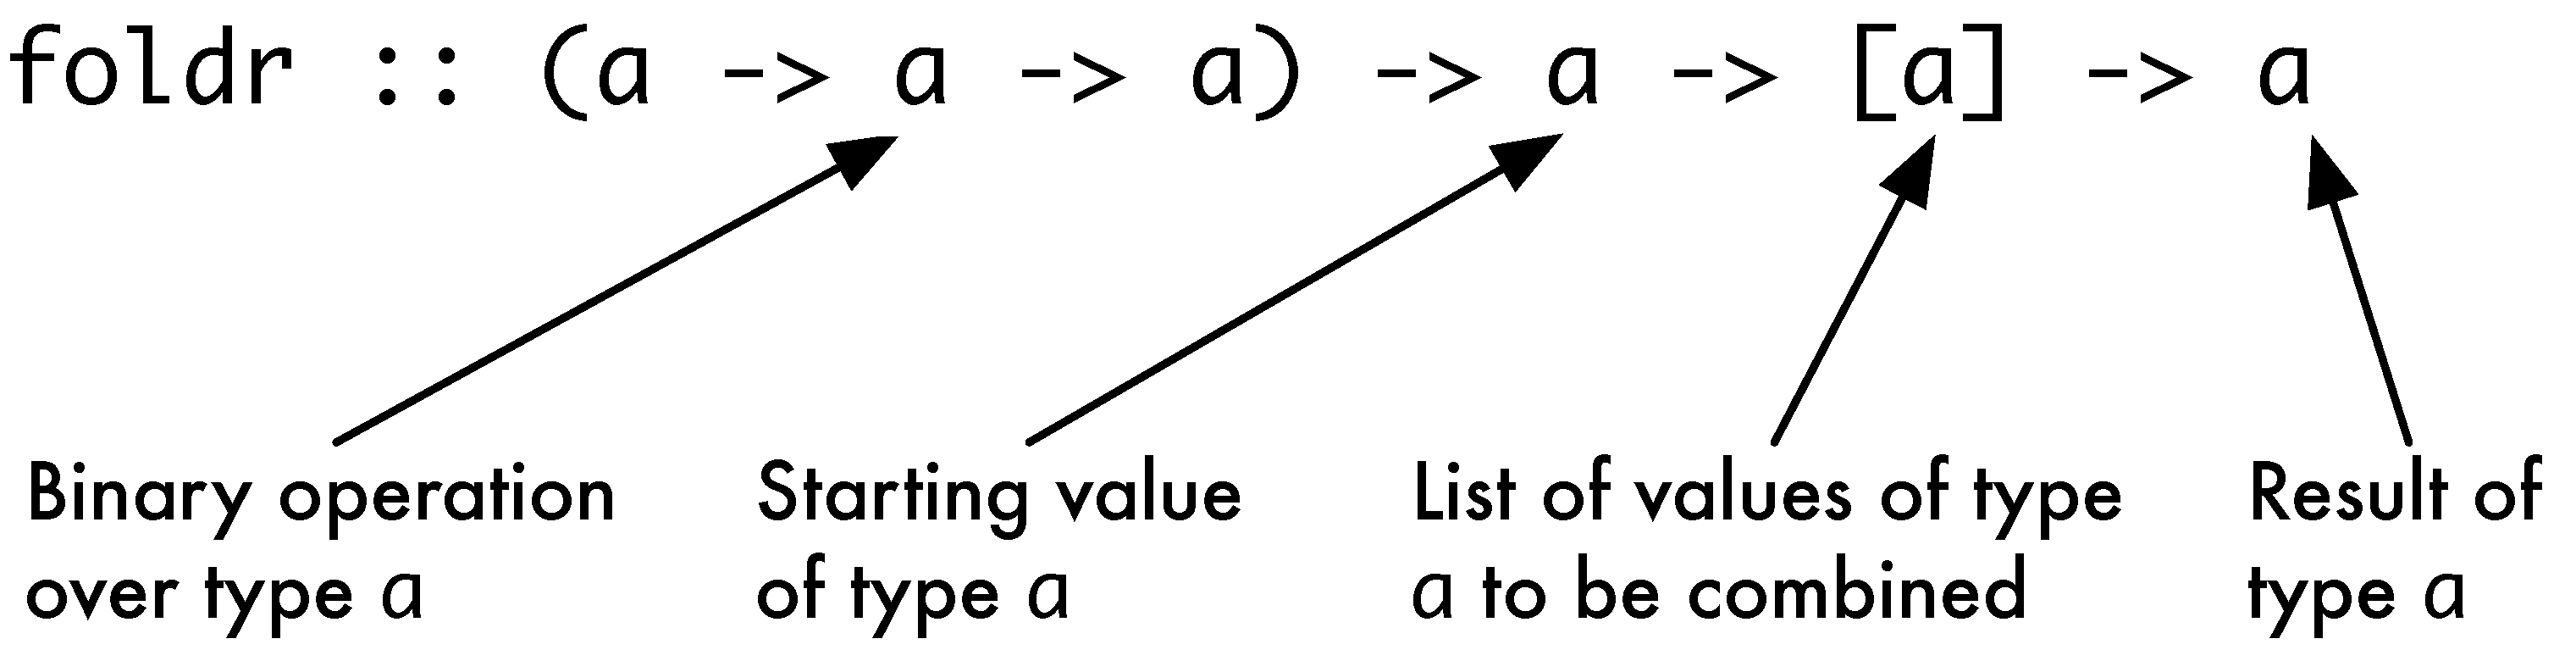
\includegraphics[width=4in]{Pictures/foldrType1.pdf}
\end{center}
we can now
define some of the standard functions of Haskell,
\begin{alltt}
concat :: [[a]] -> [a]\minx{concat}
concat xs = foldr (++) [] xs
\bl
and :: [Bool] -> Bool\minx{and}
and bs = foldr (\&\&) True bs
\end{alltt}
Returning to the start of the section, we can now see why
\texttt{foldr1} is so called: it is fold function, designed to take a
list with at least \textbf{one} element. We can also define
\texttt{foldr1} from \texttt{foldr}, like this
\begin{alltt}
foldr1 f xs = foldr f (last xs) (init xs)\hfill(foldr1.0)
\end{alltt}
where \texttt{last} gives the last element of a list, and \texttt{init} removes that element.

\subsection*{Folding in general -- \texttt{foldr} again}
\index{foldr@\texttt{foldr}}

In fact, the most general type of \texttt{foldr} is more general
than we predicted. Suppose that the starting value has type \texttt{b}
and the elements of the list are of type \texttt{a}, then
\begin{alltt}\index{foldr@\texttt{foldr}!type of}
foldr :: (a -> b -> b) -> b -> [a] -> b
\end{alltt}
We give a full explanation of how this type is derived in Section \ref{polyTypeCheck}.

With this insight about the type of \texttt{foldr} we can see
that \texttt{foldr} can be used to define another whole cohort of list functions.
For instance, we can reverse a list thus:
\begin{alltt}\minx{rev}
rev :: [a] -> [a]\minx{rev}
rev xs = foldr snoc [] xs
\bl
snoc :: a -> [a] -> [a]\minx{snoc}
snoc x xs = xs ++ [x]
\end{alltt}
This function is traditionally called \texttt{snoc} because it is like
`cons', \texttt{:},
in reverse.
We can also sort a list in this way
\begin{alltt}
iSort :: [Integer] -> [Integer]\minx{iSort}
iSort xs = foldr ins [] xs
\end{alltt}
Before we move on, we look for one last time at the definition of
\texttt{foldr}
\begin{alltt}
foldr f s []     = s\hfill(foldr.1)\index{foldr@\texttt{foldr}}
foldr f s (x:xs) = f x (foldr f s xs)\hfill(foldr.2)
\end{alltt}
What is the effect of \texttt{foldr f s}? We have two cases:
\begin{itemize}
\item the value at the empty list is given outright by \texttt{s};
\item the value at \texttt{(x:xs)} is defined in terms of the value at
\texttt{xs}, and \texttt{x} itself.
\end{itemize}
This is just like the definition of primitive recursion over
lists in Chapter \ref{defFunLists}.\footnote{There is an ambiguity in our original 
characterization. In defining the function \texttt{g} by primitive recursion the value of \texttt{g (x:xs)}
is defined in terms of both \texttt{x} and \texttt{xs} as well as the
value \texttt{g xs} itself; this makes
primitive recursion slightly more general than folding using \texttt{foldr}.}
Because of this it is no accident that we can define many of our
primitive recursive functions using \texttt{foldr}. It is usually mechanical to
go from a primitive recursive definition to the corresponding application of
\texttt{foldr}. 

How do the two approaches compare?
It is often easier initially to think of a function definition in recursive form and
only afterwards to transform it into an application of \texttt{foldr}.
One of the advantages of making this transformation is that we might
then recognize properties of the function by dint of its being a fold.
We look at proof for general functions like \texttt{map}, \texttt{filter} 
and \texttt{foldr} in Section \ref{verifGen} and we look at other fold functions in 
Chapter \ref{behaviour}.

\begin{exercises}

\item
How would you define the sum of the squares of the natural numbers \texttt{1} to
\texttt{n} using \texttt{map} and \texttt{foldr}?

\item
Define a function to give the sum of squares of the positive
integers in a list of integers.

\item
For the purposes of this exercise you should use \texttt{foldr} to
give definitions of the prelude functions
\texttt{unZip}, \texttt{last} and \texttt{init}, where examples of the
latter two
are given by\index{Peccary, Greggery}
\begin{alltt}
last "Greggery Peccary" = 'y'
init "Greggery Peccary" = "Greggery Peccar"
\end{alltt}


\item
How does the function
\begin{alltt}
mystery xs = foldr (++) [] (map sing xs)
\end{alltt}
behave, where \texttt{sing x = [x]} for all \texttt{x}?

\item
The function \texttt{formatLines} is intended to format a list of lines using the function
\begin{alltt}
formatLine :: Line -> String
\end{alltt}
to format each line in the list. Define a function 
\begin{alltt}
formatList :: (a -> String) -> [a] -> String
\end{alltt}
which takes as a parameter a function of type
\begin{alltt}
a -> String
\end{alltt}
to format each item of the list which is passed as the second parameter. Show
how \texttt{formatLines} can be defined using \texttt{formatList} and
\texttt{formatLine}.


\item
Define a function
\begin{alltt}
filterFirst :: (a -> Bool) -> [a] -> [a]
\end{alltt}
so that \texttt{filterFirst p xs} removes the first element of \texttt{xs} which does
not have the property \texttt{p}. Use this to give a version of \texttt{returnLoan}
which returns only one copy of a book. What does your function do on a list
all of whose elements have property \texttt{p}? 

\item
Can you define a function
\begin{alltt}
filterLast :: (a -> Bool) -> [a] -> [a]
\end{alltt}
which removes the last occurrence of an element of a list without property
\texttt{p}? How could you define it using \texttt{filterFirst}?



\item
How could you define a function \texttt{switchMap} which maps two functions along a list, alternating which to apply. For example,
\begin{alltt}
switchMap addOne addTen [1,2,3,4] \step{}[2,12,4,14]
\end{alltt}
where \texttt{addOne} and \texttt{addTen} behave as you would expect.
What is the most general type of \texttt{switchMap}?

\item
Define functions 
\begin{alltt}
split :: [a] -> ([a],[a])
merge :: ([a],[a]) -> [a]
\end{alltt}
so that \texttt{spilt} will split a list into two lists, picking elements alternately, while merge will interleave the two lists; for example,
\begin{alltt}
split [1,2,3,4,5] \step{}([1,3,5],[2,4])
merge ([1,3,5],[2,4]) \step{}[1,2,3,4,5]
\end{alltt}

\item
Can you formulate QuickCheck properties which characterise the way that \texttt{split} and \texttt{merge} work together?

\item {[Harder]}
Suppose that the function \texttt{g} is \emph{associative}, that is
\begin{alltt}
g x (g y z) = g (g x y) z
\end{alltt}
give a QuickCheck property that you would expect \texttt{foldr1 g (xs ++ ys)} to have. Can you think of a similar property for \texttt{foldr g s (xs ++ ys)}? Hint: you will need to think about what property \texttt{s} needs to obey.



\index{folding!and primitive recursion|)}
\index{primitive recursion!and folding|)}
\end{exercises}


\section{Generalizing: splitting up lists}
\index{generalization|(}
\index{text processing!splitting into words}

As a final example in this chapter we look at how we can generalize the
function \texttt{getWord} into a polymorphic, higher-order function.
This serves as a model for similar generalizations in many different
circumstances.

Many list manipulating programs involve splitting up lists in some way, as a
part of their processing. One way of doing this is to select some or all the
elements with a particular property -- this we have seen with \texttt{filter}.
Other ways of processing include taking or dropping elements of the list from
the front -- this we saw in the text processing example. If we know the
number of elements to be dropped, we can use
\begin{alltt}
take, drop :: Int -> [a] -> [a]\minx{take}\minx{drop}
\end{alltt}
where \texttt{take n xs} and \texttt{drop n xs} are intended to take or drop \texttt{n}
elements from the front of the list \texttt{xs}. These functions are defined in
Chapter \ref{defFunLists}.

Also in Chapter \ref{defFunLists} we looked at the example of text processing, in which
lists were split to yield words and lines. The functions 
\texttt{getWord} and \texttt{dropWord} defined there were {\em not\/} polymorphic, as they
were designed to split at whitespace characters. 

It is a general principle of functional programming that programs can often
be rewritten to use more general polymorphic and/or higher-order functions,
and we illustrate that here. 

The function \texttt{getWord} was originally defined thus:
\begin{alltt}
getWord :: String -> String\minx{getWord}
getWord []    = [] \hfill(getWord.1)
getWord (x:xs) 
  | elem x whitespace   = []\hfill(getWord.2)
  | otherwise           = x : getWord xs \hfill(getWord.3)
\end{alltt}
What forces this to work over strings is the test in \texttt{(getWord.2)}, where 
\texttt{x}
is checked for membership of \texttt{whitespace}. We can generalize the
function to have the test -- or property -- as a parameter. 

How is this to be done? Recall that a property over the type \texttt{a} is
represented by a function of type \texttt{(a -> Bool)}. Making this test a
parameter we have
\begin{alltt}
getUntil :: (a -> Bool) -> [a] -> [a]\minx{getUntil}
getUntil p []    = [] 
getUntil p (x:xs) 
  | p x         = []
  | otherwise   = x : getUntil p xs
\end{alltt}
in which the test \texttt{elem x whitespace} has been replaced by the test 
\texttt{p x}, the arbitrary property \texttt{p} applied to \texttt{x}. We can of course
recover \texttt{getWord} from this definition: 
\begin{alltt}
getWord xs 
  = getUntil p xs
    where 
    p x = elem x whitespace
\end{alltt}
\ignore{
Anticipating the next chapter a little, we can in fact write,
\begin{alltt}
getWord = getUntil (\bs{x} -> elem x whitespace)
\end{alltt}
} % end ignore
Built into Haskell are the functions \texttt{takeWhile}\minx{takeWhile}
and \texttt{dropWhile}\minx{dropWhile},
which are like \texttt{getUntil} and \texttt{dropUntil}, except that
they take or drop
elements while the condition is \texttt{True}. For instance,
\begin{alltt}
takeWhile :: (a -> Bool) -> [a] -> [a]
takeWhile p []    = [] 
takeWhile p (x:xs) 
  | p x         = x : takeWhile p xs
  | otherwise   = []
\end{alltt}
\texttt{getUntil} can be defined using \texttt{takeWhile}, and vice versa.

\index{generalization|)}


\begin{exercises}

\item
Give the type and definition of the generalization \texttt{dropUntil} of the function
\texttt{dropWord}.

\item
How would you define the function \texttt{dropSpace} using \texttt{dropUntil}?
How would you define \texttt{takeWhile}
using \texttt{getUntil}?

\item
How would you split a string into lines using \texttt{getUntil} and \texttt{dropUntil}?

\item
The function \texttt{getLine} of Chapter \ref{defFunLists} has a polymorphic type --
what is it? How could you generalize the test in this function? If you do
this, does the type of the function become more general? Explain your
answer.

\item
Can you give generalizations to polymorphic higher-order functions of the 
text processing functions \texttt{getLine}, \texttt{dropLine} and \texttt{splitLines}? 
\end{exercises}



\section{Case studies revisited}

We have already seen how the functions introduced here, \texttt{map}, \texttt{filter} and \texttt{zipWith} and so forth, can be used to re-define many of the functions from the pictures case study. This section goes back to look at other examples from that case study, as well as at others.

\subsection*{Pictures}\index{pictures}

We have discussed the \texttt{Picture} type and the functions over it already in Chapter \ref{intro}, Sections \ref{picModuleEx} and \ref{localDefs} and Chapter \ref{progLists}. In this chapter we have seen that we can define \texttt{flipV} using \texttt{map}, and \texttt{beside} using \texttt{zipWith}. The exercises that follow pick up other examples.

\begin{exercises}

\item
How can you use \texttt{map} to define the \texttt{invertColour} function, which turns a Picture into its negative?

\item
How can you use \texttt{zipWith} to define the \texttt{superimpose} function, 
\begin{alltt}
superimpose :: Picture -> Picture -> Picture
\end{alltt}
which superimposes one \texttt{Picture} (the first argument) on top of another (the second)? What does your function do if the pictures are not the same size? Can you modify your definition so that it handles this case properly?

\item {[Harder]}
Using \texttt{map} and any other functions that you need, define the function
\begin{alltt}
rotate90 :: Picture -> Picture
\end{alltt}
which rotates a picture through 90 degrees. 



\end{exercises}

\subsection*{Library database and supermarket billing}\index{library database}\index{supermarket billing}

In the database and supermarket billing examples, Sections \ref{library} and \ref{superBill}, we used list comprehensions heavily. Clearly we could have instead used \texttt{map},  \texttt{filter} and other standard list functions such as \texttt{sum}. It is a useful exercise to revisit these examples and to try re-defining some of the functions. 


\begin{exercises}

\item
Re-implement the functions
\begin{alltt}
books       :: Database -> Person -> [Book]
borrowers   :: Database -> Book -> [Person]
borrowed    :: Database -> Book -> Bool
numBorrowed :: Database -> Person -> Int
makeLoan   :: Database -> Person -> Book -> Database
returnLoan :: Database -> Person -> Book -> Database
\end{alltt}
using the functions \texttt{map},  \texttt{filter} and so on.

\item
Re-implement the functions from the previous exercise using this new definition of the 
\texttt{Database} type:
\begin{alltt}
type Database = [(Person,[Book])]
\end{alltt}

\item
Revisit the exercises of Section \ref{superBill}, where the supermarket billing example was developed, and re-implement your solutions using the prelude and library functions \texttt{map},  \texttt{filter} and so on.

\item
In the light of the previous exercises, can you come to any conclusions about when it is sensible to use list comprehensions, and when it is more useful to use the prelude and library functions explicitly?



\end{exercises}

\subsection*{Rock - Paper - Scissors}\index{Rock - Paper - Scissors}

We introduced the Rock - Paper - Scissors game in Section \ref{EnumTypes} and built on that by defining strategies in Section \ref{strategiesRPS} and showing how to play the game interactively in Section \ref{playingRPS}. 


\begin{exercises}

\item
Using the function \texttt{outcome} from Exercise 8.1 (page \pageref{outcome})
and standard list functions such as \texttt{map}, redefine the function
\begin{alltt}
tournamentOutcome :: Tournament -> Integer
\end{alltt}
described in Exercise 8.2.

\item
Redefine the function
\begin{alltt}
showTournament :: Tournament -> String
\end{alltt}
first introduced on page \pageref{showTournament}, using the standard list functions introduced in this chapter.



\end{exercises} 



\begin{summary}
This chapter has shown how the informal patterns of definition over
lists can be realized as higher-order, polymorphic functions, such as
\texttt{map}, \texttt{filter} and \texttt{foldr}. We saw how these
functions arose, and also how their types were derived, as well as
reviewing the ways in which they could be used to solve problems.

Next we looked at an example of how to generalize a function -- the
particular example was taken from the text processing case study, but
the example serves as a model for how to generalize functions in
general. The chapter concludes with a re-examination of some of the case studies.

The chapter has focused on how to write functions which take other
functions as arguments; where do these arguments come from? One answer
is that they are already defined; another is that they come themselves
as the results of Haskell functions -- this is the topic of the next
chapter.

\end{summary}


%\end{document}

%\documentclass{book}\usepackage{sjtfonts}\usepackage{includegraphics}\usepackage{alltt}\usepackage{latexsym}
%\usepackage{array}
%\begin{document}\input{defs0}%		miradefs.tex 		    June 1994

% opening and closing a quoted Miranda section

\newcommand{\mira}{\noindent\hrulefill\nopagebreak\so}
\newcommand{\arim}{\nopagebreak\st\hrulefill\\}

% backslash in the Miranda environment
% Only feasible approach is to use \verb+\+
% in line!

%\newcommand{\bs}{$\mi\backslash\!\!$}
%\newcommand{\lbs}{\mbox{\verb+\+}}

% ignoring part of the input

\newcommand{\ignore}[1]{}

% a blank line in a Miranda section

\newcommand{\bl}{\mbox{\ }}

% Signalling a diffculty.

\definecolor{light-gray}{gray}{0.95}

\newcommand{\beware}[2]
 {\medskip\noindent\colorbox{light-gray}{\parbox{\textwidth}
 {\mbox{\large\textbf{#1}} \medskip\noindent\\ #2}\medskip\noindent}}

% Subscripting in Miranda text
\newcommand{\subscr}[2]{\mbox{${\mbox{\texttt{#1}}}_{\mbox{\texttt{#2}}}$}}

%\newcommand{\subscr}[2]{\mbox{${\mbox{\mi #1}}_{\mbox{\smtt #2}}$}}
\newcommand{\aone}{\subscr{a}{1}}
\newcommand{\atwo}{\subscr{a}{2}}
\newcommand{\ak}{\subscr{a}{k}}

\newcommand{\aoneone}{\subscr{a}{1,1}}

\newcommand{\eone}{\subscr{e}{1}}
\newcommand{\etwo}{\subscr{e}{2}}
\newcommand{\ei}{\subscr{e}{i}}
\newcommand{\er}{\subscr{e}{r}}

\newcommand{\fone}{\subscr{f}{1}}
\newcommand{\fl}{\subscr{f}{l}}

\newcommand{\gone}{\subscr{g}{1}}
\newcommand{\gtwo}{\subscr{g}{2}}
\newcommand{\gi}{\subscr{g}{i}}
\newcommand{\gr}{\subscr{g}{r}}

\newcommand{\hone}{\subscr{h}{1}}
\newcommand{\hl}{\subscr{h}{l}}

\newcommand{\pone}{\subscr{p}{1}}
\newcommand{\ptwo}{\subscr{p}{2}}
\newcommand{\pk}{\subscr{p}{k}}

\newcommand{\qone}{\subscr{q}{1}}
\newcommand{\qtwo}{\subscr{q}{2}}
\newcommand{\qk}{\subscr{q}{k}}

\newcommand{\rone}{\subscr{r}{1}}
\newcommand{\rtwo}{\subscr{r}{2}}

\newcommand{\tone}{\subscr{t}{1}}
\newcommand{\ttwo}{\subscr{t}{2}}
\newcommand{\tn}{\subscr{t}{n}}

\newcommand{\vone}{\subscr{v}{1}}
\newcommand{\vtwo}{\subscr{v}{2}}
\newcommand{\vn}{\subscr{v}{n}}

% for regular expressions

\newcommand{\stone}{\subscr{st}{1}}
\newcommand{\sttwo}{\subscr{st}{2}}
\newcommand{\stn}{\subscr{st}{n}}
\newcommand{\rthree}{\subscr{r}{3}}

\newcommand{\eps}{$\varepsilon$}
\newcommand{\trans}[1]{\stackrel{\mbox{\tt #1}}{\longrightarrow}}



% superscript in Miranda text

\newcommand{\superscr}[2]{\mbox{${\mbox{\mi #1}}^{\mbox{\smtt #2}}$}}

% Not equals in Miranda text

\newcommand{\noteq}{\makebox[0pt][l]{=}/}
\newcommand{\overslash}{\makebox[0pt][l]{/}}

% Definitions in complexity chapter

\newfont{\oldSym}{cmsy10}
\newcommand{\Th}{\boldmath$\oldSym\Theta$}
\newcommand{\pow}[1]{\^{}#1}
\newcommand{\leqq}{$\leq$}
\newcommand{\geqq}{$\geq$}
\newcommand{\lll}{$\ll$}
\newcommand{\eqq}{$\equiv$}
\newcommand{\ltwo}{\subscr{log}{2}}

% Indexing

\newcommand{\minx}[1]{\index{#1@{\ttfamily{}#1}}}
\setcounter{chapter}{9}\setcounter{page}{157}


\chapter{Higher-order functions}
\chapstart
\label{gen2}
\index{higher-order function}

Haskell is a \emph{functional} programming language: that means that the main way in which we compute things is by defining functions which describe how to transform the inputs into the required output. Haskell has a collection of built-in data types which we can use to model the data in the problem domain, including numbers, booleans, lists, tuples and \texttt{data} types.

Haskell is also functional in a more distinctive way: \emph{functions are data} in Haskell, and can be treated just like data of any other type. \index{function!as data}
\begin{itemize}
\item
Functions can be combined using \emph{operators}, just like the numbers can be combined using the arithmetical operators.
\item
Haskell provides \emph{lambda abstractions}, which allow us to describe functions directly by expressions, rather than having to define and name a function in order to use it.
\item
Functions can be the inputs and outputs of other functions in exactly the same way as any other type. Functions which have other functions as arguments or results are called \emph{higher-order functions}.
\item
In particular, the syntax of Haskell makes it particularly easy to \emph{partially apply} functions and operators, so that functions are returned as the results of applying functions.
\end{itemize}
This chapter covers these topics, setting the scene for Chapter \ref{developingHOPs} where will put these ideas into practice.

Finally, we'll also see that we can start to write function-level definitions -- sometimes called `point-free' definitions -- which can be more concise, more readable and more suitable for program verification and transformation. Indeed, the chapter concludes with
some examples of program verification involving higher-order polymorphic
functions, and we see there that the theorems proved about them are reusable in
exactly the same way that the functions themselves are reusable.


\section{Operators: function composition and application}

This section describes the built-in operators for function composition and application, as well as defining a new operator, forward composition, which composes functions in the `natural' order.

\subsection*{Function composition: \texttt{.}}
\index{function composition|(}

\begin{figure}[t]
\begin{center}
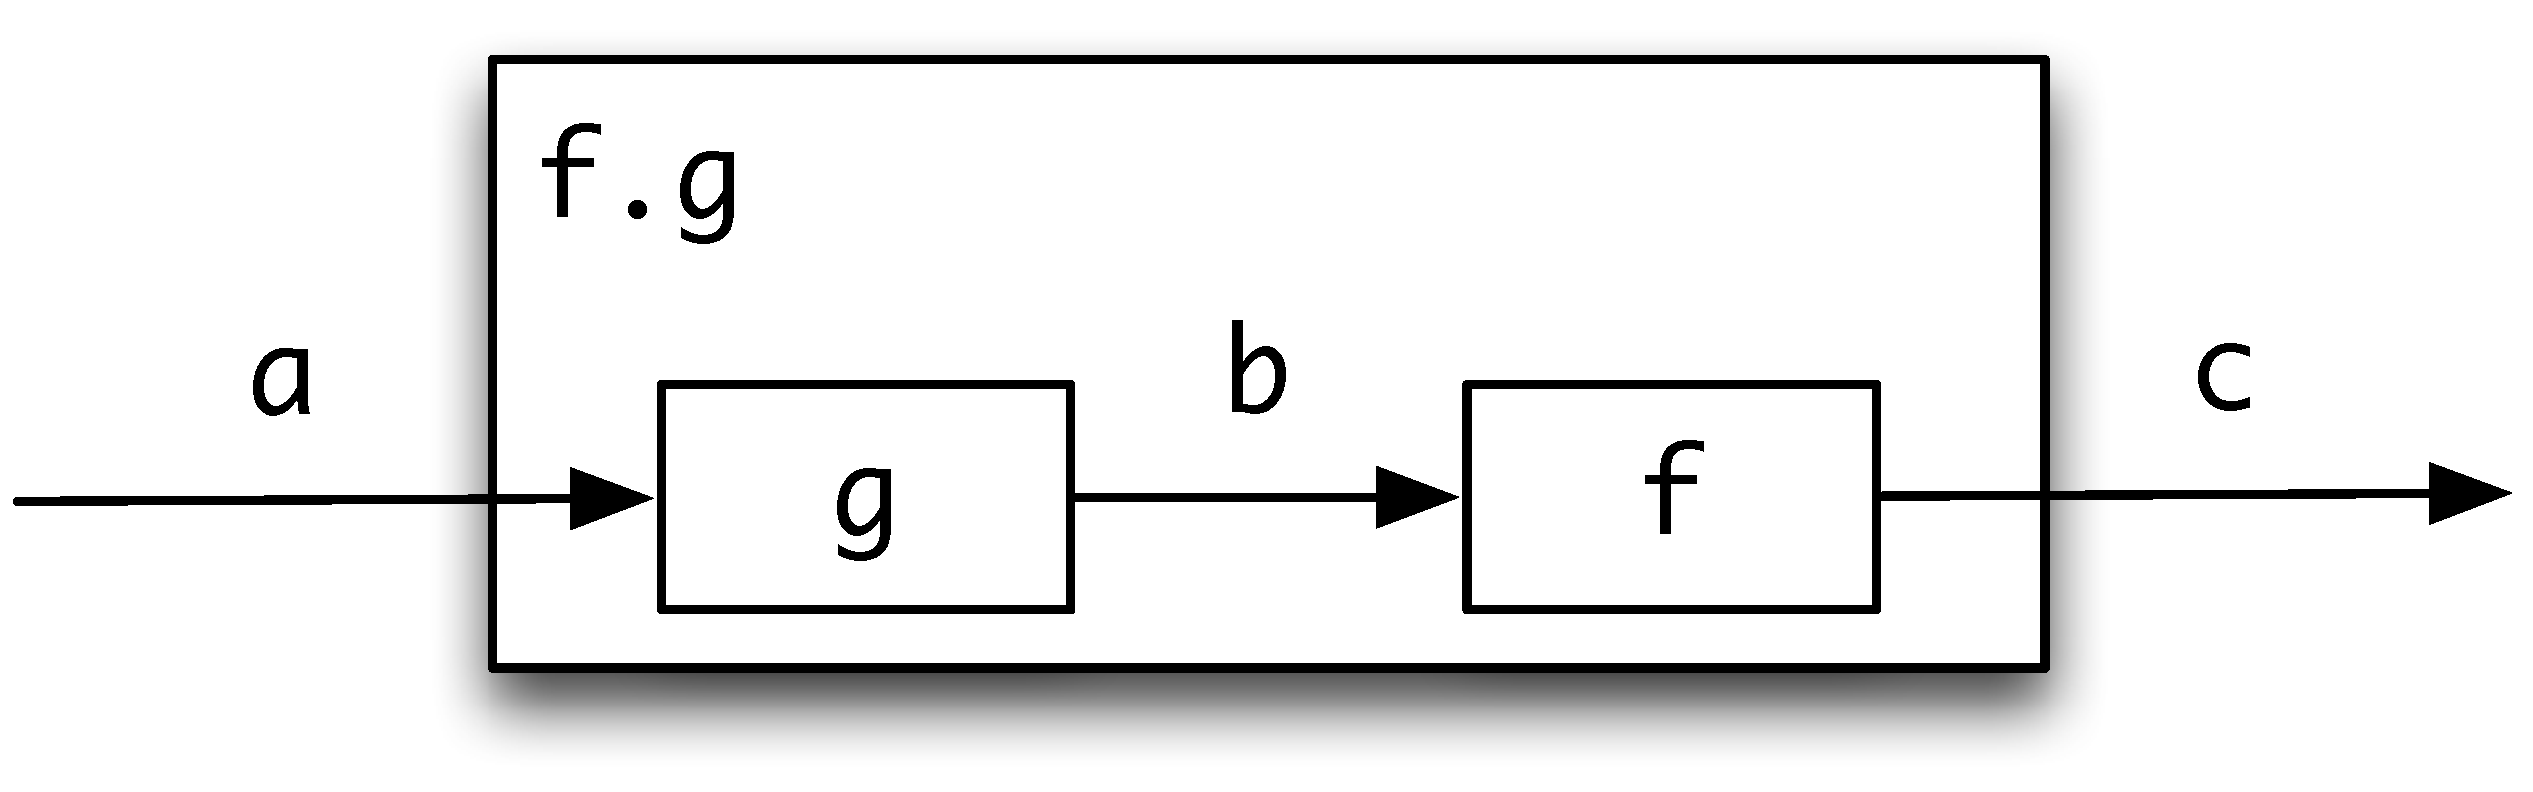
\includegraphics[width=3in]{Pictures/compos.pdf}
\end{center}
\caption{Function composition}
\label{funComp}
\end{figure}

Function composition is one of the simplest ways of structuring a program: do a number of things
one after the other: each part can be designed and implemented separately. 

Haskell has the \textbf{function composition}  operator over functions built in. The operator, which is denoted by the `\texttt{.}' between the two functions, has the effect of `wiring together' two functions: passing the output of one to the input of another, and it is .  This is pictured in Figure \ref{funComp}, where the annotations of the arrows in the diagram
indicate the types of elements involved.


For any functions \texttt{f} and \texttt{g}, the effect of \texttt{f.g} is given by
the definition
\begin{alltt}
(f.g) x = f (g x)\hfill(comp.1)
\end{alltt}
Not all pairs of functions can be composed. The output of \texttt{g}, \texttt{g x},
becomes the input of \texttt{f}, so that the output type of \texttt{g} must equal
the input type of \texttt{f}. 

Recalling the \texttt{Picture} example, we have already seen a definition of \texttt{rotate}:
\begin{alltt}\minx{rotate}
rotate :: Picture -> Picture
rotate pic = flipV (flipH pic)\hfill(rotate.1)
\end{alltt}
Using the composition operator we can say directly that \texttt{rotate} is the composition of \texttt{flipH} with \texttt{flipV}:
like
\begin{alltt}
rotate = flipV . flipH\hfill(rotate.2)
\end{alltt}
Notice that we explained the definition \texttt{(rotate.2)} as the `composition of \texttt{flipH} with \texttt{flipV}': why that way round? We do this because \texttt{flipH} is the function that is applied first, with \texttt{flipV} being applied to the result of the first application. We are able to compose \texttt{flipH} with \texttt{flipV} because the output of
\texttt{flipH} and the input of \texttt{flipV} are both of 
\texttt{Picture} type.



In general, the constraint on which functions can be composed 
is expressed by giving `\texttt{.}' the type
\begin{center}
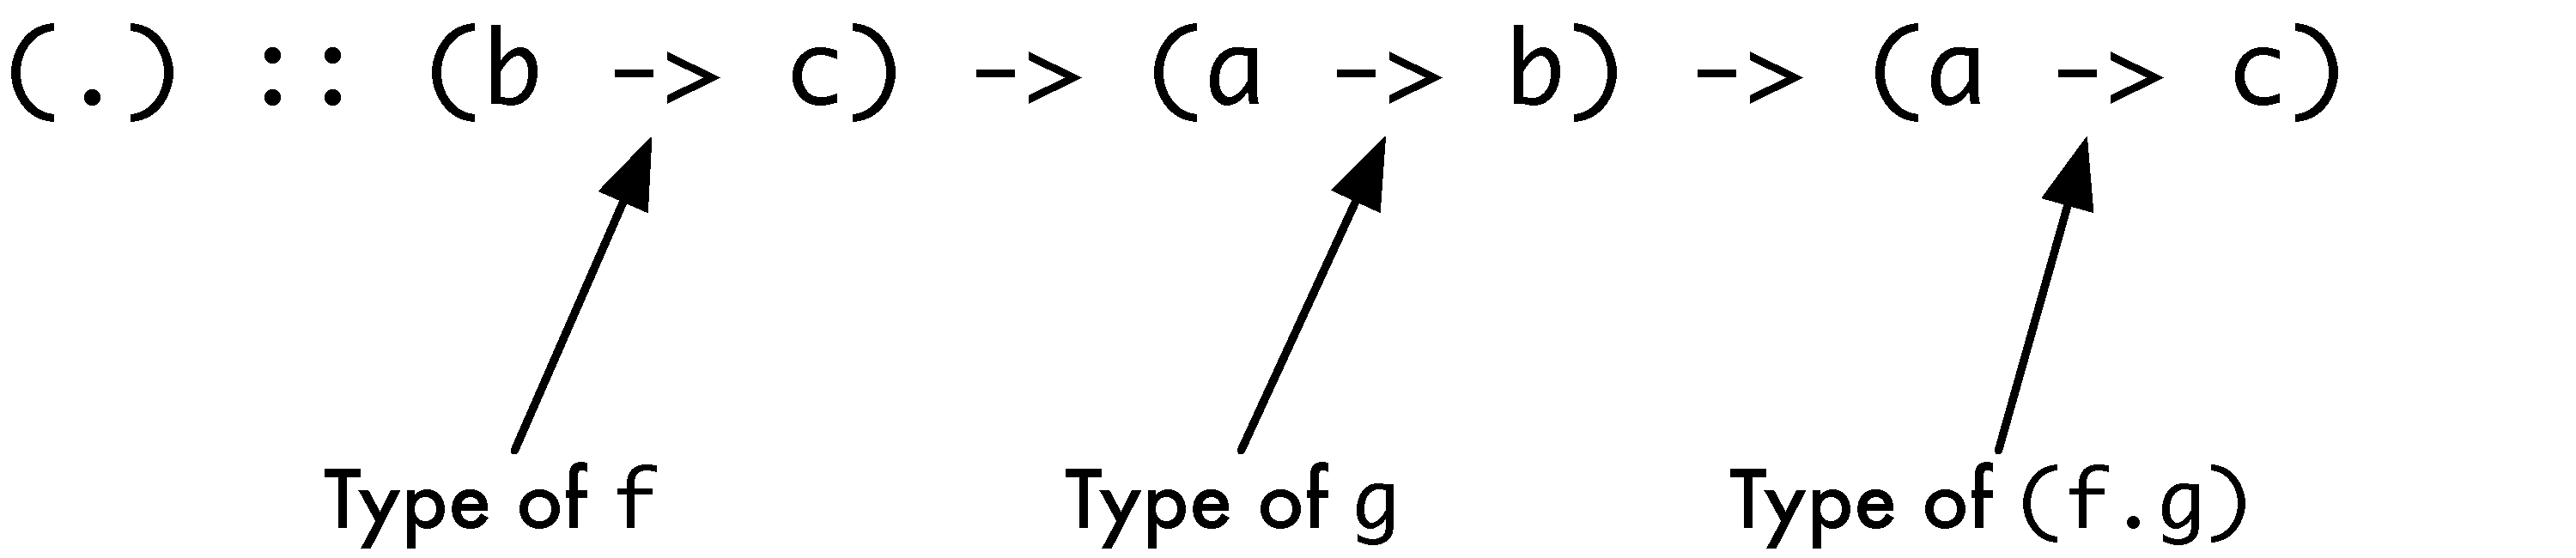
\includegraphics[width=3.5in]{Pictures/composType.pdf}
\end{center}\index{function composition!type of}
which shows that, if we call the first input \texttt{f} and the second \texttt{g}, 
\begin{titemize}
\item The input of \texttt{f} and the output of \texttt{g} are of the same type: 
\texttt{b}.
\item The result \texttt{f.g} has the same input type, \texttt{a}, as \texttt{g} and 
the same output type, \texttt{c}, as \texttt{f}.
\end{titemize}
Composition is {\bf associative}, that is \index{associativity}
\texttt{f.(g.h) } is equal to \texttt{(f.g).h} for all \texttt{f}, \texttt{g} and 
\texttt{h}. We can therefore write \texttt{f.g.h} unambiguously to mean `do \texttt{h}, then
\texttt{g}, then \texttt{f}'.\footnote{For technical reasons, the `\texttt{.}'
is treated as right associative in the Haskell standard prelude.}


\begin{figure}[t]\index{function composition!binding power of}
\beware{The `binding power' of composition}{
There is a common error caused by the binding powers of
function application and function composition. 

It is an error to write \texttt{f.g x} thinking it
means \texttt{(f.g)} applied to \texttt{x}. Because function application binds more
tightly than anything else, it is interpreted by the system
as \texttt{f.(g x)}, which will often lead to a type
error. 
For example, evaluating 
\begin{alltt}
not.not True
\end{alltt}
gives the type error message
\begin{alltt}
\ \ \ \ Couldn't match expected type `a -> Bool'

\ \ \ \ \ \ \ \ \ \ \ \ against inferred type `Bool'

\ \ \ \ In the second argument of `(.)', namely `not True'

\ \ \ \ In the expression: not . not True

\ \ \ \ In the definition of `it': it = not . not True
\end{alltt}
since there is an attempt to treat \texttt{not True} as a function to be composed
with \texttt{not}. Such a function needs to have type \texttt{a -> Bool}, 
whereas it actually has type \texttt{Bool}. 

In applying a composition we therefore need to be sure that it is
\textbf{parenthesized} like this:
\begin{alltt}
(not.not) True
\end{alltt}
}
\end{figure}


\subsection*{Forward composition: \texttt{>.>}}
\index{forward composition}
\index{function composition!forward}

The order in \texttt{f.g} is significant, and can be confusing; \texttt{(f.g)}
means `first apply \texttt{g} and then apply \texttt{f} to the result', so the function that is applied first comes second in the composition.


It is simple in Haskell to define an operator for composition which takes its
arguments in the opposite order to `\texttt{.}', like this:
\begin{alltt}\index{\symbol{62}\symbol{46}\symbol{62}@\texttt{\symbol{62}\symbol{46}\symbol{62}}}
infixl 9 >.>
\bl
(>.>) :: (a -> b) -> (b -> c) -> (a -> c)
\bl
g >.> f = f . g\hfill(fcomp.1)
\end{alltt}
This definition has the effect that
\begin{alltt}
(g >.> f) x = (f.g) x = f (g x)\hfill(fcomp.2)
\end{alltt}
showing that, as it were, the order of the \texttt{f} and \texttt{g} is swapped
before the functions are applied.
The \texttt{rotate} example can then be written
\begin{alltt}\minx{rotate}
rotate = flipH >.> flipV  
\end{alltt}
which we can read as \texttt{flipH} {\em then\/} \texttt{flipV}, with the
functions being applied \emph{from left to right}. 

The notation `\texttt{>.>}' contains a `\texttt{.}' to show that it is a form of
composition, with the arrows showing the direction in which information is
flowing. We will tend to use `\texttt{>.>}' in situations where a number
of functions are composed, and it is therefore tiresome to read some
lines down the page in order to work out the effect of a function
definition.





\index{function composition|)}

\subsection*{The application operator: \texttt{\$}}\minx{\$}\index{application operator (\texttt{\$})}

We're familiar in Haskell with how to write the application of a function \texttt{f} to an argument \texttt{e}: we just write \texttt{f} next to \texttt{e}, like this: \texttt{f e}. In other words, we \textbf{juxtapose} the function and its argument.

We can also explicitly write down an application using the application operator, `\texttt{\$}', like this: \texttt{f \$ e}. Why on earth would we want to do this, when we can write it without the `\texttt{\$}'? There are two reasons that an explicit application gets used:
\begin{itemize}
\item
Many Haskell programmers use `\texttt{\$}' as an alternative to parentheses, so you may well see this in libraries that people have written. 
Instead of writing something like
\begin{alltt}
flipV (flipH (rotate horse))
\end{alltt}
it is possible to write:
\begin{alltt}
flipV $ flipH $ rotate horse
\end{alltt}
with the same meaning. Arguably this is a little clearer, and it is shorter! Incidentally you can see from this example that `\texttt{\$}' is \textbf{right associative}.
\item
We need to use the application operator as a function, as in the example
\begin{alltt}
zipWith ($) [sum,product] [[1,2],[3,4]] 
\end{alltt}
where the application operator is applied to corresponding elements of the two lists.\end{itemize}

\begin{figure}[t]\index{application operator (\texttt{\$})!and composition}\index{function composition!and application (\texttt{\$})}
\beware{Application and composition}{
Application and composition can get confused. Function composition combines two functions,
while application combines a function and an argument (which can be a
function, of course).
\itempar
If, for example, 
\texttt{f} has type \texttt{Integer -> Bool}, then
\begin{itemize}
\item[--]
\texttt{f.x} means \texttt{f} composed with the {\em function\/} \texttt{x}; \texttt{x}
therefore needs to be of type \texttt{s~->~Integer} for some type \texttt{s}.  
\item[--]
\texttt{f x} means \texttt{f} applied to the object \texttt{x}, so \texttt{x} must
therefore be an integer.
\item[--]
\texttt{f \$ x} also means \texttt{f} applied to the object \texttt{x}, and so \texttt{x} must
again be an integer.
\end{itemize}
}
\end{figure}




\begin{exercises}

\item
Redefine the function \texttt{printBill} from the supermarket billing exercise
in Section \ref{superBill} so that composition is used. Repeat the exercise using
forward composition, \texttt{>.>}.

\item
If \texttt{id} is the polymorphic identity function, defined by 
\texttt{id x = x}, explain the
behaviour of the expressions 
\begin{alltt}
(id.f)         (f.id)         id f
\end{alltt}If \texttt{f} is of type
\texttt{Int -> Bool}, at what instance of its most general type \texttt{a -> a}
is \texttt{id} used in each case? What type does
\texttt{f} have if \texttt{f id} is properly typed?

\item
Define a function \texttt{composeList} which composes a list of
functions into a single function. You should give the
type of \texttt{composeList}, and explain why the function has this
type. What is the effect of your function on an empty list of functions?


\item
What is the type of the application operator, \texttt{\$}?

\item
What is the result of the expression given above:
\begin{alltt}
zipWith ($) [sum,product] [[1,2],[3,4]] 
\end{alltt}

\item
If \texttt{id} is the polymorphic identity function, defined by 
\texttt{id x = x}, explain the
behaviour of the expressions 
\begin{alltt}
(id \$ f)         (f \$ id)         id (\$)
\end{alltt}If \texttt{f} is of type
\texttt{Int -> Bool}, at what instance of its most general type \texttt{a -> a}
is \texttt{id} used in each case? What type does
\texttt{f} have if \texttt{f \$ id} is properly typed?





\end{exercises}



\section{Expressions for functions: lambda abstractions}
\label{exprFuns}

Haskell definitions give us a way of defining functions, and once we have defined a function we can use its name to refer to it, as in the application
\begin{alltt}
map addOne [2,3,4]
\end{alltt}
assuming that we've already defined
\begin{alltt}
addOne x = x+1
\end{alltt}
Haskell gives us a way of writing down an expression that means `the function that adds one to a number' directly, without having to give it a name. We write
\begin{alltt}
\bs{}x -> x+1
\end{alltt}
which we can read as saying `the function  that takes \texttt{x} to \texttt{x+1}', the initial `\bs{}' signalling that it's a function. So, we can add one to all the numbers in the list \texttt{[2,3,4]} by writing the expression
\begin{alltt}
map (\bs{}x -> x+1) [2,3,4]
\end{alltt}
An expression like \texttt{(\bs{}x -> x+1)} is called a \emph{lambda abstraction}.\index{lambda abstraction} 

\beware{Why is a called a `lambda abstraction'?}{The `lambda' comes from the lambda calculus, a
mathematical theory of functions. The symbol `\texttt{\bs{}}' is the closest
ASCII character to the Greek character lambda, $\lambda$, used in the $\lambda$-calculus. One of the inventors of the $\lambda$-calculus was Haskell B.\ Curry, after whom Haskell is named. 

The `abstraction' comes from the fact that the expression \texttt{(\bs{x} -> e)} is a function, which `abstracts away' from the particular expression \texttt{e}.}

\subsection*{Examples of lambda abstractions}

Let's take a look at some other uses of this notation now. Suppose that we want to take a list of functions and apply them all to a particular argument,
\begin{alltt}
mapFuns :: [a->b] -> a -> [b]
\end{alltt}
giving a list of results. We might do this in playing a game of Rock - Paper - Scissors  where we apply a number of different strategies to the current game position, and then compare the different results; we'll come back to this scenario later in the chapter.

We could define the function by recursion, like this:
\begin{alltt}
mapFuns [] x     = []
mapFuns (f:fs) x = f x : mapFuns fs x
\end{alltt}
but in fact we can use \texttt{map} in making the definition: what we have to do at each element of the list (remember, each element is a function) is to apply it to \texttt{x}, so
\begin{alltt}
mapFuns fs x = map (\bs{}f -> f x) fs
\end{alltt}
What's important to see here is that the function \texttt{(\bs{}f -> f x)} depends on the  value of \texttt{x}, and so we cannot define it as a top level function. We could, alternatively, define it in a \texttt{where} clause,
\begin{alltt}
mapFuns fs x = map applyToX fs
			   where
			   applyToX f = f x
\end{alltt}
The first definition is clearer, and defines the operative function directly, rather than having to name and define it in a \texttt{where} clause, separately from where it is used; of course, either is OK, and it's a matter of taste which you might use.  

One of the main uses of lambda abstractions is to define functions which are the results of functions. Let's look at the example of the function
\begin{alltt}
addNum :: Integer -> (Integer -> Integer)
\end{alltt}
The function takes an integer, 17 say, and returns a function: in this case the function that adds 17 to its argument. The definition says this directly:
\minx{->}\minx{addNum}
\begin{alltt}
addNum n = (\bs{m} -> n+m)
\end{alltt}

\subsection*{`Plumbing' functions together}

Another example which uses a lambda abstraction is given by the
`plumbing' illustrated in Figure \ref{plumb}.
\begin{figure}[t]
\begin{center}
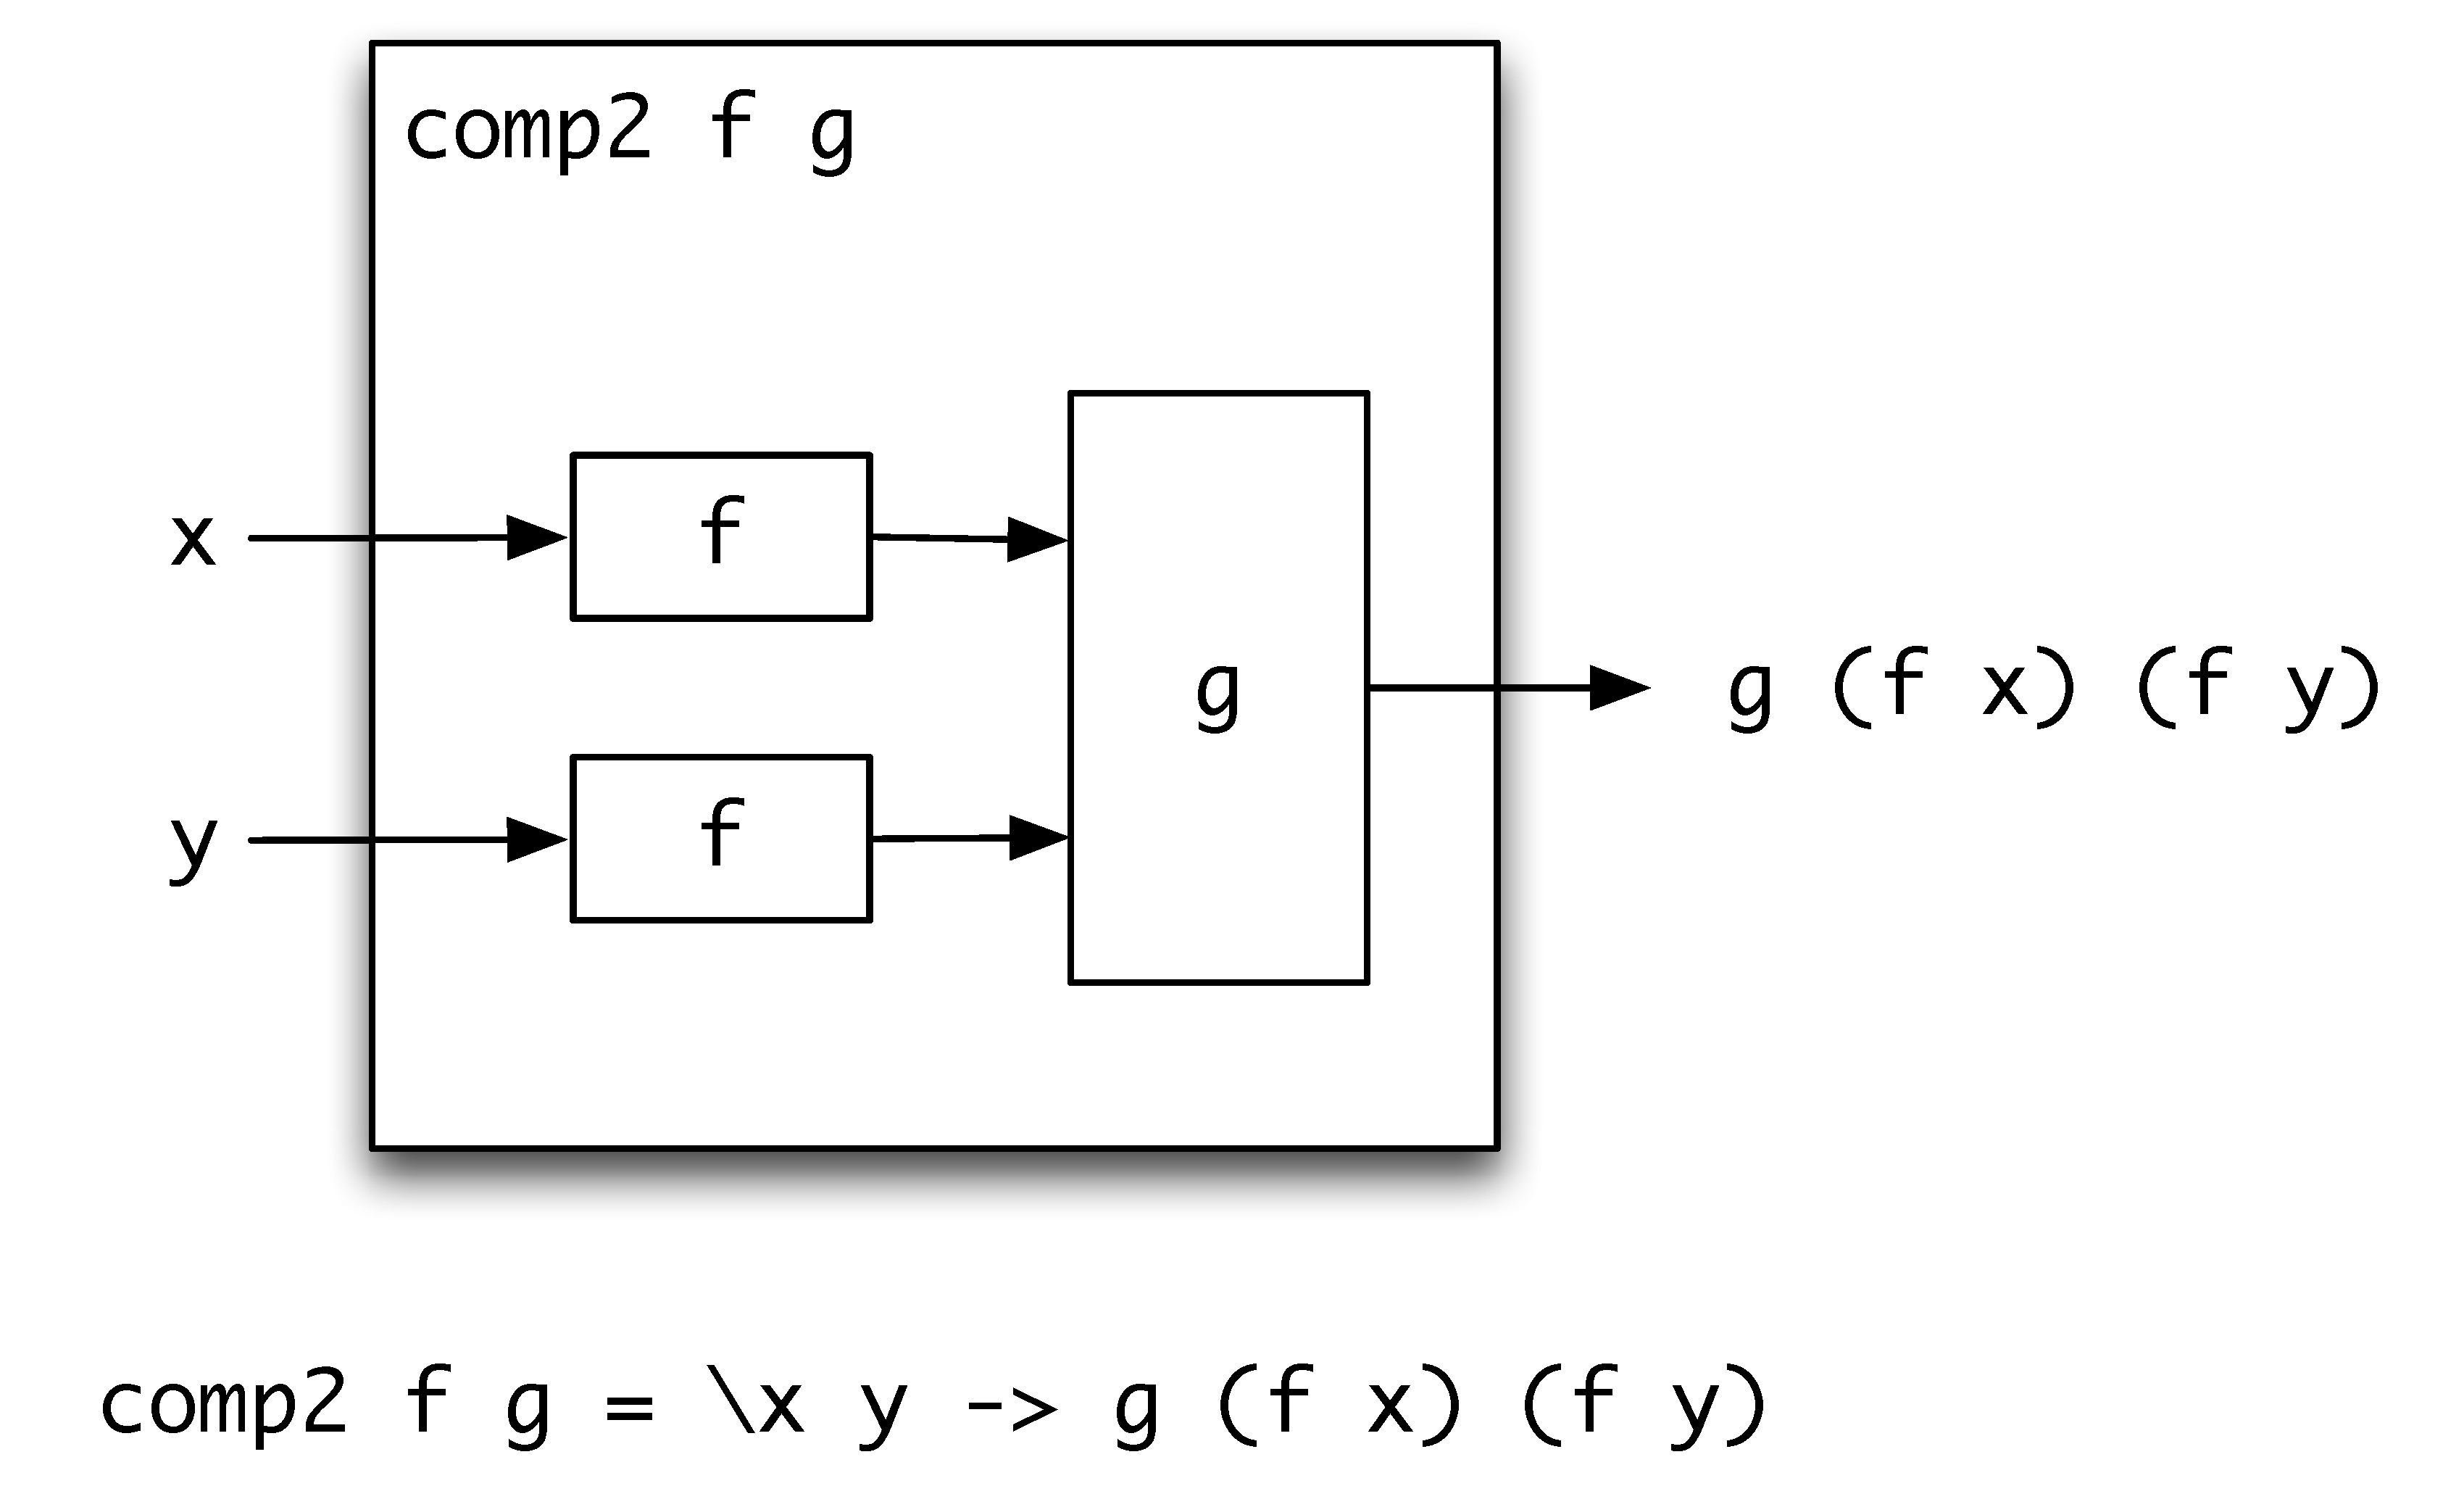
\includegraphics[width=4in]{Pictures/comp2.pdf}
\end{center}
\caption{Plumbing \texttt{f} and \texttt{g} together.}
\label{plumb}\index{plumbing}
\end{figure}
The object shown
is a function, whose arguments are \texttt{x} and \texttt{y}. The result 
of the function is 
\begin{alltt}
g (f x) (f y)
\end{alltt}
so the overall effect is to give a
function which applies \texttt{f} to each of its (two) arguments before applying
\texttt{g} to the results. Again, the definition states this directly:
\begin{alltt}\minx{comp2}
comp2 :: (a -> b) -> (b -> b -> c) -> (a -> a -> c)
\bl
comp2 f g = (\bs{x} y -> g (f x) (f y))
\end{alltt}
To add together the squares of \texttt{3} and \texttt{4} we can write
\begin{alltt}
comp2 sq add 3 4
\end{alltt}
where \texttt{add} and \texttt{sq} have the obvious definitions.

In general, a lambda abstraction is an \textbf{anonymous}
version\index{function!anonymous}
of the sort of function we have defined earlier. In other words, the
function \texttt{f} defined by
\begin{alltt}
f x y z = result
\end{alltt}
and the function
\begin{alltt}
\bs{}x y z -> result
\end{alltt}
have exactly the same effect.

We shall see in the next
section that partial application will make many definitions -- including some
of the functions here -- more straightforward. On the other hand the
lambda abstraction is more general, and thus can be used in situations when
a partial application could not.

\begin{exercises}

\item
Using a lambda abstraction, the Boolean function \texttt{not}
and the built-in function \texttt{elem}
describe a function of type
\begin{alltt}
{\hskip1pc}Char -> Bool
\end{alltt}
which is \texttt{True} only on non-whitespace characters, that is those which are
not elements of the list \texttt{" \bs{t}\bs{n}"}.

\item
Define a function \texttt{total}
\begin{alltt}
{\hskip1pc}total :: (Integer -> Integer) -> (Integer -> Integer)
\end{alltt}
so that \texttt{total f} is the function which at value \texttt{n} gives the total
\begin{alltt}
{\hskip1pc}f 0 + f 1 + \ldots + f n
\end{alltt}
You should be able to do this using built-in functions, rather than using recursion.

\item
Given a function \texttt{f} of type \texttt{a -> b -> c}, write down a lambda abstraction that
describes
the function of type \texttt{b -> a -> c} which behaves like \texttt{f} but
which takes its arguments in the other order. Pictorially,
\begin{center}
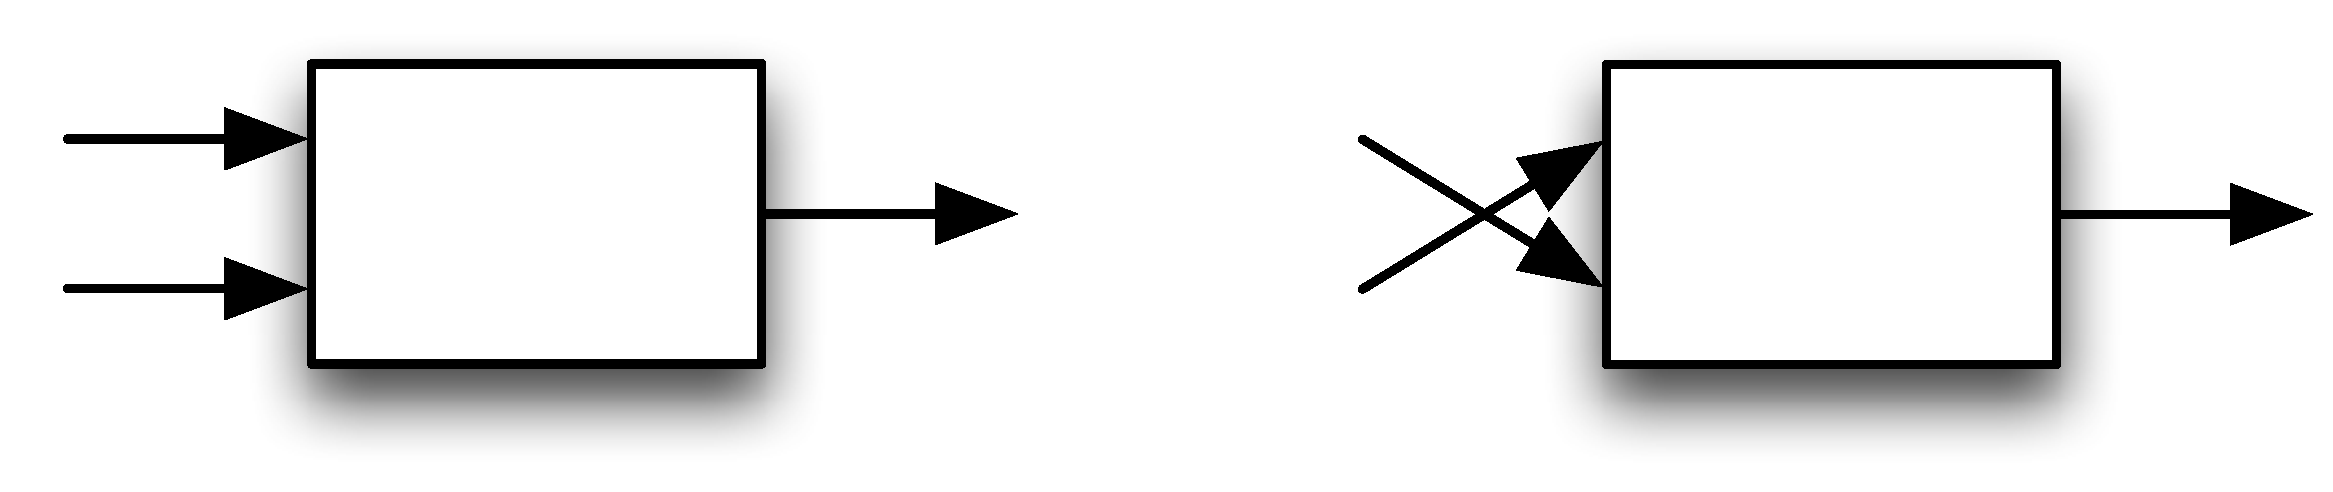
\includegraphics[width=3.4in]{Pictures/flip.pdf}
\end{center}


\item
Using the last exercise, or otherwise, give a definition of the function
\begin{alltt}
{\hskip1pc}{\hskip1pc}flip :: (a -> b -> c) -> (b -> a -> c)
\end{alltt}
which reverses the order in which its function argument takes its arguments.


\end{exercises}







\section{Partial application}\index{partial application|(}
\index{function application!partial|see{partial application}}


In this section we'll discover how it is possible to \emph{partially apply} functions in Haskell, and what the effect of this is. Underlying the Haskell approach to functions is what is called the \emph{curried} representation of functions, in honour of Haskell Curry; this is introduced in the section after this. 

\subsection*{Introducing partial application}


The function \texttt{multiply} multiplies together two arguments,
\begin{alltt}
multiply :: Int -> Int -> Int\minx{multiply}
multiply x y = x*y
\end{alltt}
We can view the function as a box, with two input arrows and an output arrow.
\begin{center}
\mbox{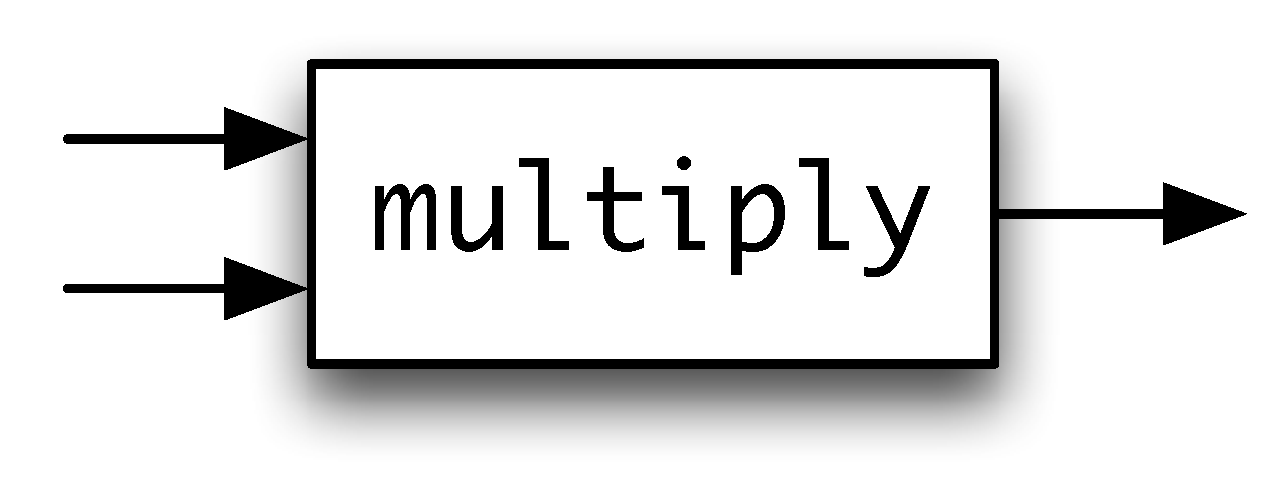
\includegraphics[height=1.5cm]{Pictures/mult1.pdf}}
\end{center}
If we apply the function to two arguments, the result is a number;
so that, for instance, \texttt{multiply 2 3} equals \texttt{6}. 
\begin{center}
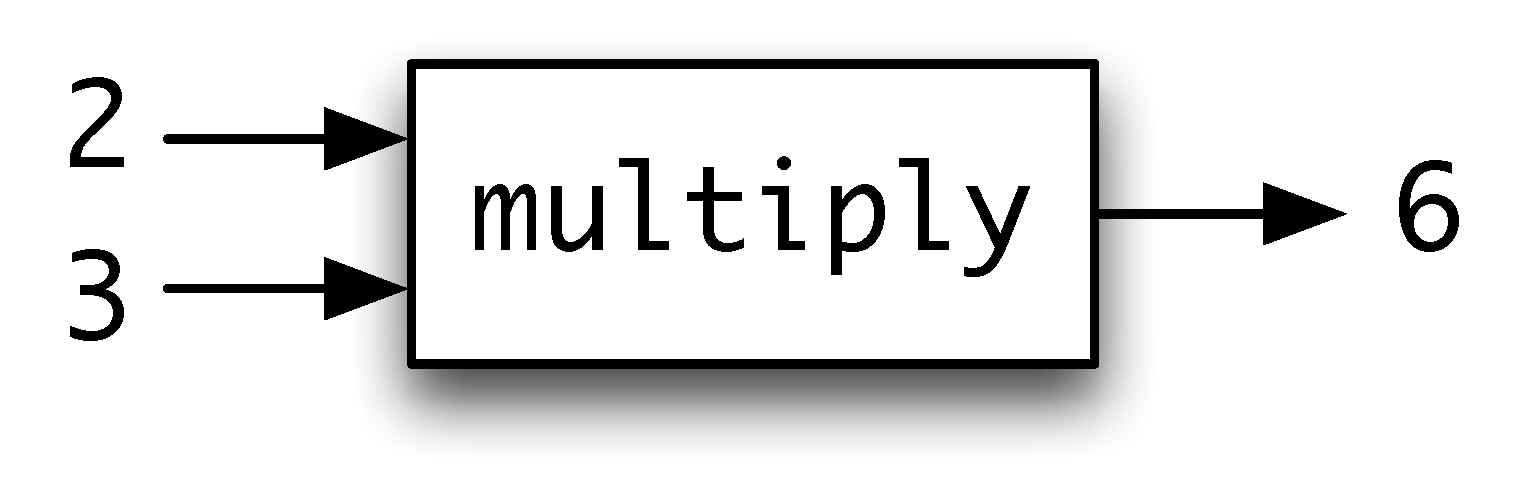
\includegraphics[height=1.5cm]{Pictures/mult2.pdf}
\end{center}
What happens if \texttt{multiply} is
applied to \textbf{one} argument \texttt{2}? Pictorially, we have
\begin{center}
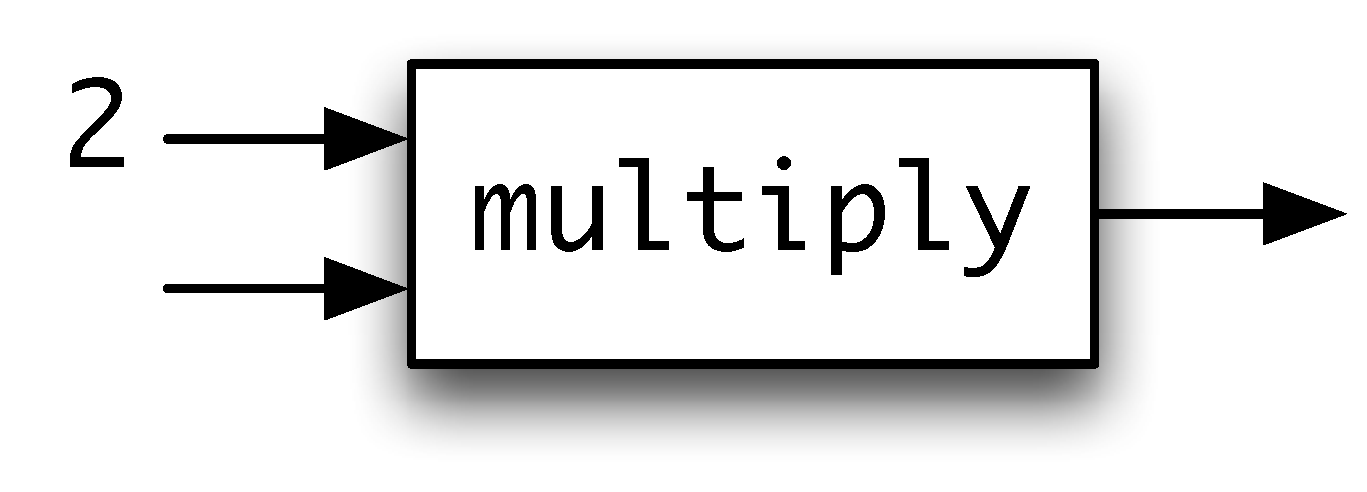
\includegraphics[height=1.5cm]{Pictures/mult3.pdf}
\end{center}
From the picture we can see that this represents a function, as there is 
still one input arrow to the function awaiting a value. This function 
will, when given the awaited argument \texttt{y}, return double its value, namely \texttt{2*y}.

This is an example of a general phenomenon: any function taking two or more
arguments can be \textbf{partially applied} to one or more arguments. This gives
a powerful way of forming functions as results. 



\subsection*{Example: the \texttt{doubleAll} function}


\noindent
To illustrate, we at the example of the function which doubles every element in a list of integers. The function can be defined like this:
\begin{alltt}
doubleAll :: [Int] -> [Int]\minx{doubleAll}
doubleAll = map (multiply 2)
\end{alltt}
In this definition there are two partial applications:
\begin{titemize}
\item \texttt{multiply 2} is a function from integers to integers, given by
applying \texttt{multiply} to one rather than two arguments;
\item \texttt{map (multiply 2)} is a function from \texttt{[Int]} to \texttt{[Int]},
given by partially applying \texttt{map}.
\end{titemize}
Partial application is being put to two different uses here.
\begin{titemize}
\item In the first case -- \texttt{multiply 2} -- the partial
application is used to form the function which
multiplies by two, and which is passed to \texttt{map} to form
the \texttt{doubleAll} function.
\item the second partial application -- of \texttt{map} to
\texttt{multiply 2} -- could be avoided by writing the argument to \texttt{doubleAll} 
\begin{alltt}
doubleAll xs = map (multiply 2) xs
\end{alltt}
but it is quite possible to write a \emph{function level} definition like this, and it is shorter and clearer than the definition with the arguments supplied.
\end{titemize}
In Section \ref{exprFuns} we saw the example of \texttt{addNum}, 
\begin{alltt}\minx{addNum}
addNum n = (\bs{m} -> n+m)
\end{alltt}
which when applied to an integer \texttt{n}
was intended to return the function which adds \texttt{n} to its
argument. With partial application we have a simpler mechanism, as we
can say
\begin{alltt}
addNum n m = n+m
\end{alltt}
since when \texttt{addNum} is applied to one argument \texttt{n} it returns the 
function adding \texttt{n} to its argument.

\begin{figure}[t]\index{argument!order of arguments}
\beware{Order of arguments}{
It is not always possible to make a partial application, since the argument to
which we
want to apply the function may not be its first argument.
Let's look at the function
\begin{alltt}\minx{elem}
elem :: Char -> [Char] -> Bool
\end{alltt}
We can test whether a character \texttt{ch} is a whitespace character by writing
\begin{alltt}
elem ch whitespace
\end{alltt}
where \texttt{whitespace} is the string
\texttt{" \bs{t}\bs{n}"}. We would like to write the function to test this by
partially applying \texttt{elem} to \texttt{whitespace}, but cannot, because this is the secdon argument rather than the first.

One solution is to define
a variant of \texttt{elem} which takes its arguments in the other order, as in
\begin{alltt}\minx{member}
member xs x = elem x xs
\end{alltt}
and write the function as the partial application 
\begin{alltt}
member whitespace
\end{alltt} 
Alternatively, we can
write down this function as a lambda abstraction, like this:
\begin{alltt}
\bs{ch} -> elem ch whitespace
\end{alltt}
}\end{figure}


\subsection*{Partially applied operators: operator sections}
\index{operator sections}
\label{opsecs}

The operators of the language can be partially applied, giving what are
known as {\bf operator sections}. Examples include

\medskip
\noindent
\begin{mytable}
\ttfamily (+2) & The function which adds two to its argument.\\
\ttfamily (2+) & The function which adds two to its argument.\\
\ttfamily (>2) & The function which returns whether a number is greater
than two.\\
\ttfamily (3:) & The function which puts the number \texttt{3} on the front of a
list.\\
\ttfamily (++"\bs{n}") & The function which puts a newline at the end of a string.\\
\ttfamily ("\bs{n}"++) & The function which puts a newline at the beginning of a string.\\ 
\ttfamily (\$ 3) & The function which applies its argument -- which will have to be a function -- to the integer \texttt{3}.\\ 
\end{mytable}

\medskip
\noindent
The general rule here is that a section of the operator \texttt{op} will put
its argument to the side which completes the application. That is, 
\begin{alltt}
(op x) y = y op x
(x op) y = x op y
\end{alltt}
When combined with higher-order functions like \texttt{map}, 
\texttt{filter} and composition, the notation is both powerful and elegant, 
enabling us to make a whole lot more function-level definitions. For example,
\begin{alltt}
filter (>0) . map (+1)
\end{alltt}
is the function which adds one to each member of a list, and then removes those
elements which are not positive.

\begin{figure}[t]\index{parentheses!different roles in Haskell}
\beware{Parentheses in Haskell}{
The main role of parentheses, \texttt{(} \ldots \texttt{)}, in Haskell is to group items together so that the system interprets what you have written in the right way. Typical examples include
\begin{titemize}
\item
enclosing a pattern in a definition, as in \texttt{sum (Node t1 t2) = \ldots};
\item
enclosing a negative literal in a function application, as in \texttt{fac (-1)};
\item
enclosing a type annotation, as in \texttt{foldr plus (1::Int) [1..1000]};
\item
overriding the binding power of operators, as in \texttt{(2+3)*6};
\item
grouping names in a \texttt{deriving} clause like \texttt{deriving (Eq, Show)
}.
\end{titemize}
However, other uses of parentheses have an effect of building data elements or changing the meaning of an identifier.
\begin{titemize}
\item
To form a tuple, it is necessary to enclose the items in parentheses, as in \texttt{(1,True)}; the notation \texttt{1,True} on its own is meaningless.
\item
To turn an infix operator into a prefix operator, it must be enclosed in parentheses, as in \texttt{(\&\&)}.
\item
To form an operator section, the operator and arguments are enclosed in parentheses as seen in this example: \texttt{(\&\& True).(0 /=).(`rem` 2)}.
\end{titemize}
}
\end{figure}

\subsection*{Using partial applications}

The partial application and operator sections is important in Haskell programming. We have already seen that
many functions can be defined as {\bf specializations} of general operations
\index{specialization}
like \texttt{map}, \texttt{filter} and so on. These specializations arise by
passing a function to the general operation -- this function is often
given by a partial application, as in the examples from the pictures
case study first seen in Chapter \ref{intro}:
\begin{alltt}\minx{flipV}\minx{beside}
flipV  = map reverse
beside = zipWith (++)
\end{alltt}
We return to look at the \texttt{Picture} case study in greater detail
in Section \ref{hofPicture}.

More examples of partial applications will be seen throughout the material to
come, and can be used to simplify and clarify many of the preceding examples.
Three simple examples are the text processing functions we first looked at in Section \ref{textProc}:
\begin{alltt}
dropSpace = dropWhile (member whitespace)\minx{dropSpace}
dropWord  = dropWhile (not .\ member whitespace)\minx{dropWord}
getWord   = takeWhile (not .\ member whitespace)\minx{getWord}
\end{alltt}
where
\begin{alltt}
member xs x = elem x xs
\end{alltt}
 
\begin{exercises}


\item
Use partial applications to define the functions \texttt{comp2} and
\texttt{total} given in Section \ref{exprFuns} and its exercises.

\item
Find operator sections \texttt{\subscr{sec}{1}} and
\texttt{\subscr{sec}{2}} so that
\begin{alltt}
map \subscr{sec}{1} . filter \subscr{sec}{2}
\end{alltt}
has the same effect as
\begin{alltt}
filter (>0) .\ map (+1)
\end{alltt}


\item
Re-define the function \texttt{mapFuns}, first defined in Section \ref{exprFuns}, using an operator section of the application operator, \texttt{\$}.
\end{exercises}

\section{Under the hood: curried functions}

Functions in Haskell are represented in \textbf{curried} form, where they take their arguments one at a time.
This
\index{Curry, Haskell B.}
is called {\bf currying} after Haskell Curry\footnote{In fact the first
person to describe the idea was Sch\"{o}nfinkel, but `Sch\"{o}nfinkeling' does
not sound so snappy!} who was one of the pioneers of 
the $\lambda$-calculus and after whom the Haskell language is named. This section explains how curried functions work, and how we can covert to and fro between curried and uncurried form.

Why are Haskell functions in curried form? A major reason is that it supports partial application, as explored in the previous section; it also gives a `clean' readable form to the syntax. One reason against choosing a curried representation is its unfamiliarity to most programmers; another is discussed towards the end of the section.

\index{partial application|)}

\subsection*{Curried functions and function arguments}
\index{function!number of arguments}

\index{partial application}
Partial application can appear confusing: in some contexts functions appear
to take one argument, and in others more than one. In fact, {\em every function in
Haskell takes exactly one argument}. This is called the \textbf{curried} representation of functions.If this application yields a function,
then this function may be applied to a further argument, and so on.
Consider the multiplication
function again. 
\begin{alltt} 
multiply :: Int -> Int -> Int\minx{multiply}
\end{alltt}
This is shorthand for
\begin{alltt} 
multiply :: Int -> (Int -> Int)
\end{alltt}
and so it can therefore be applied to an integer. Doing this
gives (for example)
\begin{alltt}
multiply 2 :: Int -> Int
\end{alltt}
This can
itself be applied to give
\begin{alltt}
(multiply 2) 5 :: Int
\end{alltt}
which, since function application is left associative, can be written 
\begin{alltt}
multiply 2 5 :: Int
\end{alltt}
Our explanations earlier in the book are consistent with this full explanation
of the system. We hid the fact that
\begin{alltt}
f \eone \etwo \ldots \subscr{e}{k}
\tone -> \ttwo -> \ldots \tn -> t
\end{alltt}
were shorthand for
\begin{alltt}
( \ldots((f \eone) \etwo) \ldots \subscr{e}{k})
\tone -> (\ttwo -> (\ldots(\tn -> t)\ldots))
\end{alltt}
but this did no harm to our understanding of how to use the Haskell
language. It is to support this shorthand that function application is
made left associative and \texttt{->} is made right associative.

\begin{figure}[t]
\beware{The syntax of application and \texttt{->}}{\index{function application!syntax}\index{syntax!of application}Function application is {\bf left associative} so
that
\texttt{f x y} means \texttt{(f x) y}, \emph{not} \texttt{f (x y)}.

\medskip
The function space symbol `\texttt{->}'\minx{->} is {\bf right
associative}, so that \texttt{a -> b -> c} means
\texttt{a~->~(b~->~c)}, \emph{not}
\texttt{(a~->~b)~->~c}.}
\end{figure}

\begin{figure}[t]\index{associativity!arrow not associative}
\beware{The arrow is not associative.}{Functions \texttt{f ::\ Int -> Int -> Int} and 
\texttt{g ::\ (Int -> Int) -> Int} are illustrated here
\begin{center}
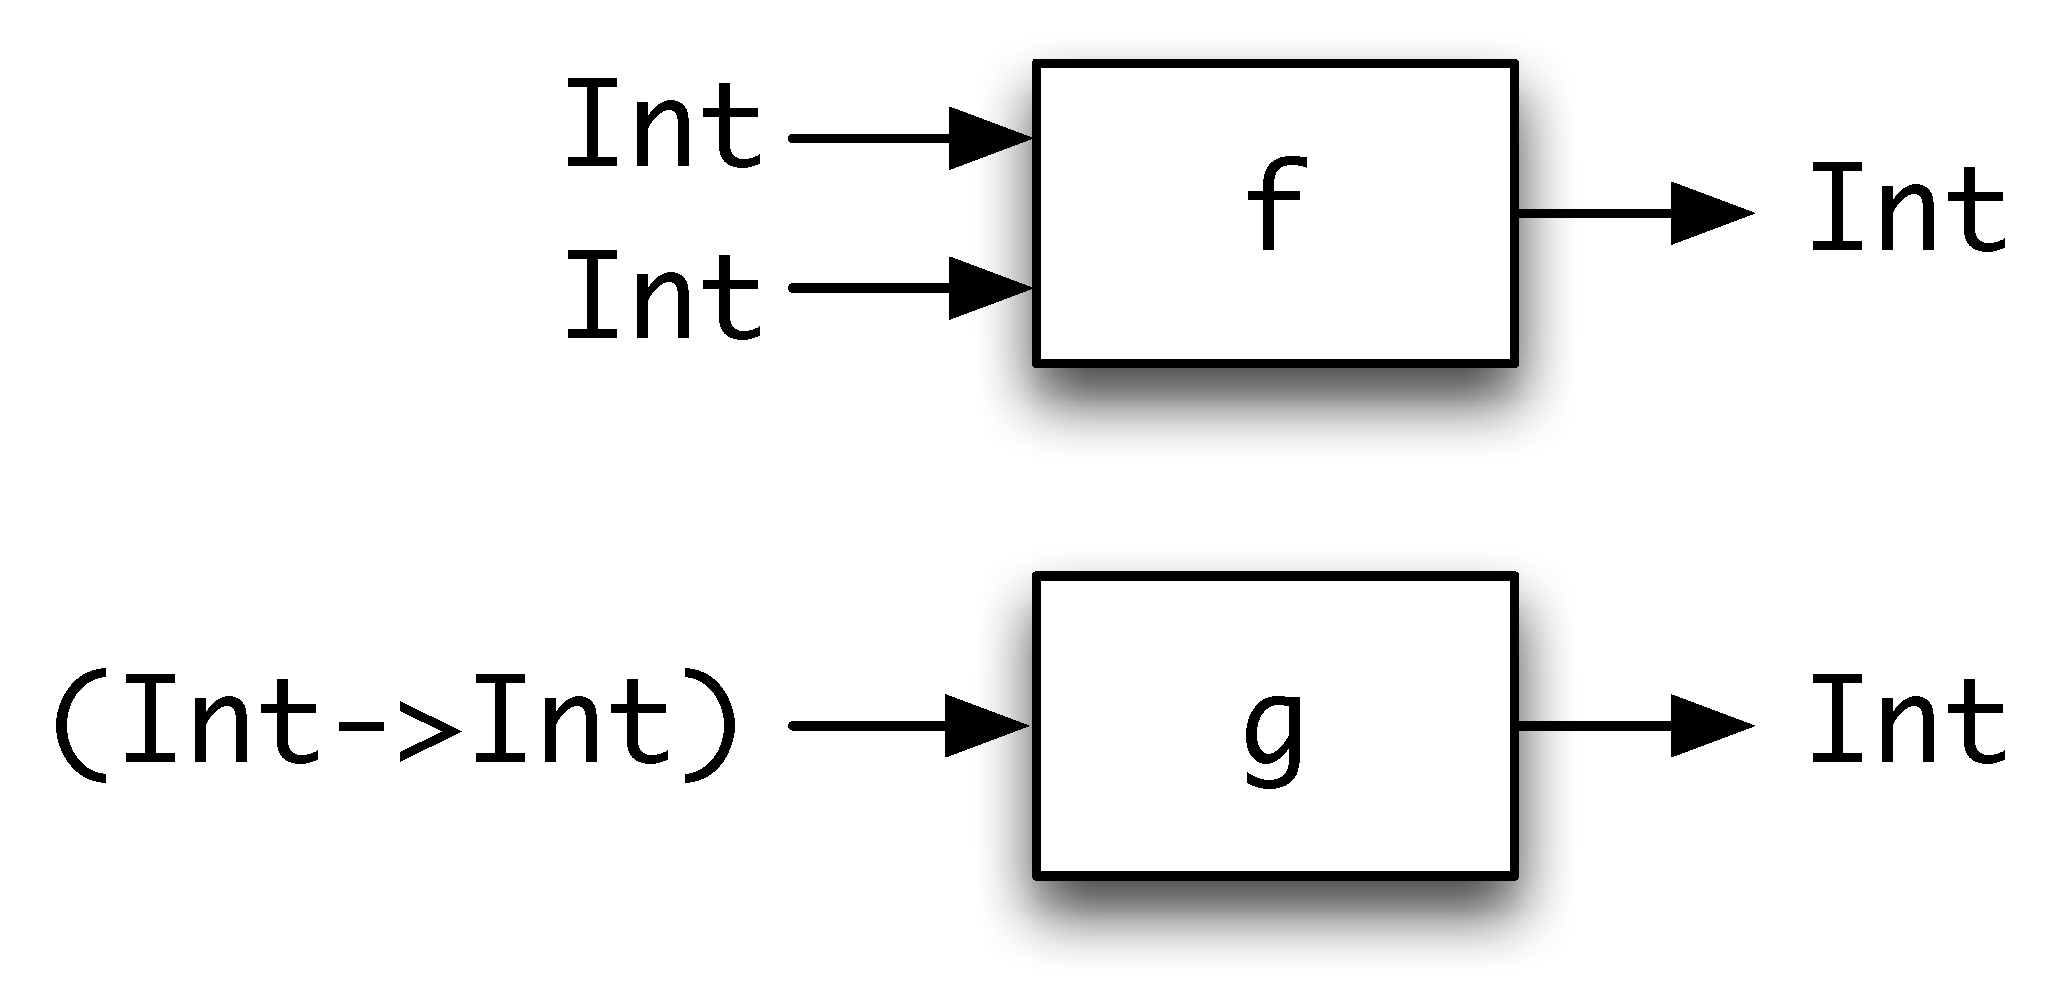
\includegraphics[width=3.0in]{Pictures/arrowDiags.pdf}
\end{center}
The function \texttt{f} will yield a
function from \texttt{Int} to \texttt{Int} when given a \texttt{Int} -- an example is
\texttt{multiply}. 
On the other hand,
when given a function of type \texttt{Int -> Int},
\texttt{g} yields a \texttt{Int}.
An example is
\begin{alltt}
g :: (Int -> Int) -> Int

g h = (h 0) + (h 1)
\end{alltt}
The function \texttt{g} defined here takes a function \texttt{h} as argument and
returns the sum of \texttt{h}'s values at \texttt{0} and \texttt{1}, and
so \texttt{g succ} will have the value \texttt{3}.
}\end{figure}

\subsection*{The types of partial applications}
\index{partial application!type of}

How is the type of a partial application determined? There
is a simple rule which explains it.

\begin{definition}{%
{\sffamily Rule of cancellation}
\medskip

\index{type checking!rule of cancellation}

\begin{quote}
If the type of a function \texttt{f} is
\begin{alltt}
{\hskip1pc}\tone -> \ttwo -> ... -> \tn -> t
\end{alltt}
and it is applied to arguments
\begin{alltt}
{\hskip1pc}\eone::\tone, \etwo::\ttwo, \ldots, \subscr{e}{k}::\subscr{t}{k}
\end{alltt}
(where$\;$\texttt{k$\leq$n})$\;$then$\;$the$\;$result$\;$type$\;$is$\;$given$\;$by$\;${\bf cancelling}$\;$the$\;$types$\;$\texttt{\tone}$\;$to~\subscr{t}{k}

\begin{alltt}
{\hskip1pc}\makebox[0pt][l]{/}\tone -> \makebox[0pt][l]{/}\ttwo -> ... -> \makebox[0pt][l]{/}\subscr{t}{k}-> \subscr{t}{k+1} -> ... -> \tn -> t
\end{alltt}
which gives the type
\begin{alltt}
{\hskip1pc}\subscr{t}{k+1} -> \subscr{t}{k+2} -> ... -> \tn -> t
\end{alltt}\end{quote}}
\end{definition}


\noindent
For example, using this rule we can see that we get the following types
\begin{alltt}
multiply 2      :: Int -> Int
multiply 2 3    :: Int
doubleAll       :: [Int] -> [Int]
doubleAll [2,3] :: [Int]
\end{alltt}


\subsection*{Currying and uncurrying}
\label{curry}
\index{function!curried|see{currying}}
\index{currying|(}

In Haskell we have a choice of how to model functions of two or more
arguments.  For
instance, a function to multiply two integers would normally be defined
thus:
\begin{alltt}\minx{multiply}
multiply :: Int -> Int -> Int
multiply x y = x*y
\end{alltt}
while an {\bf uncurried}\index{uncurrying} version 
can be given by bundling the arguments into a pair, thus:
\begin{alltt}\minx{multiplyUC}
multiplyUC :: (Int,Int) -> Int
multiplyUC (x,y) = x*y
\end{alltt}
Why do we usually opt for the curried form? There are a number of
reasons.
\begin{titemize}\index{currying!reasons for}
\item The notation is somewhat neater; we apply a function to a single
argument by juxtaposing the two, \texttt{f x}, and application to two arguments 
is done by extending this thus: \texttt{g x y}.
\item It permits partial application.\index{partial application!and currying} 
In the case of multiplication we
can write expressions like \texttt{multiply 2}, which returns a
function, while this is not possible if the two arguments are bundled
into a pair, as is the case for \texttt{multiplyUC}.
\end{titemize}
We can in any case move between the 
curried and uncurried representations with little difficulty, and indeed we 
can define
two higher-order functions which convert between curried and
uncurried functions.

Suppose first that we want to write a curried version of a function
\texttt{g}, which is itself uncurried and of type \texttt{(a,b) -> c}.
\begin{center}
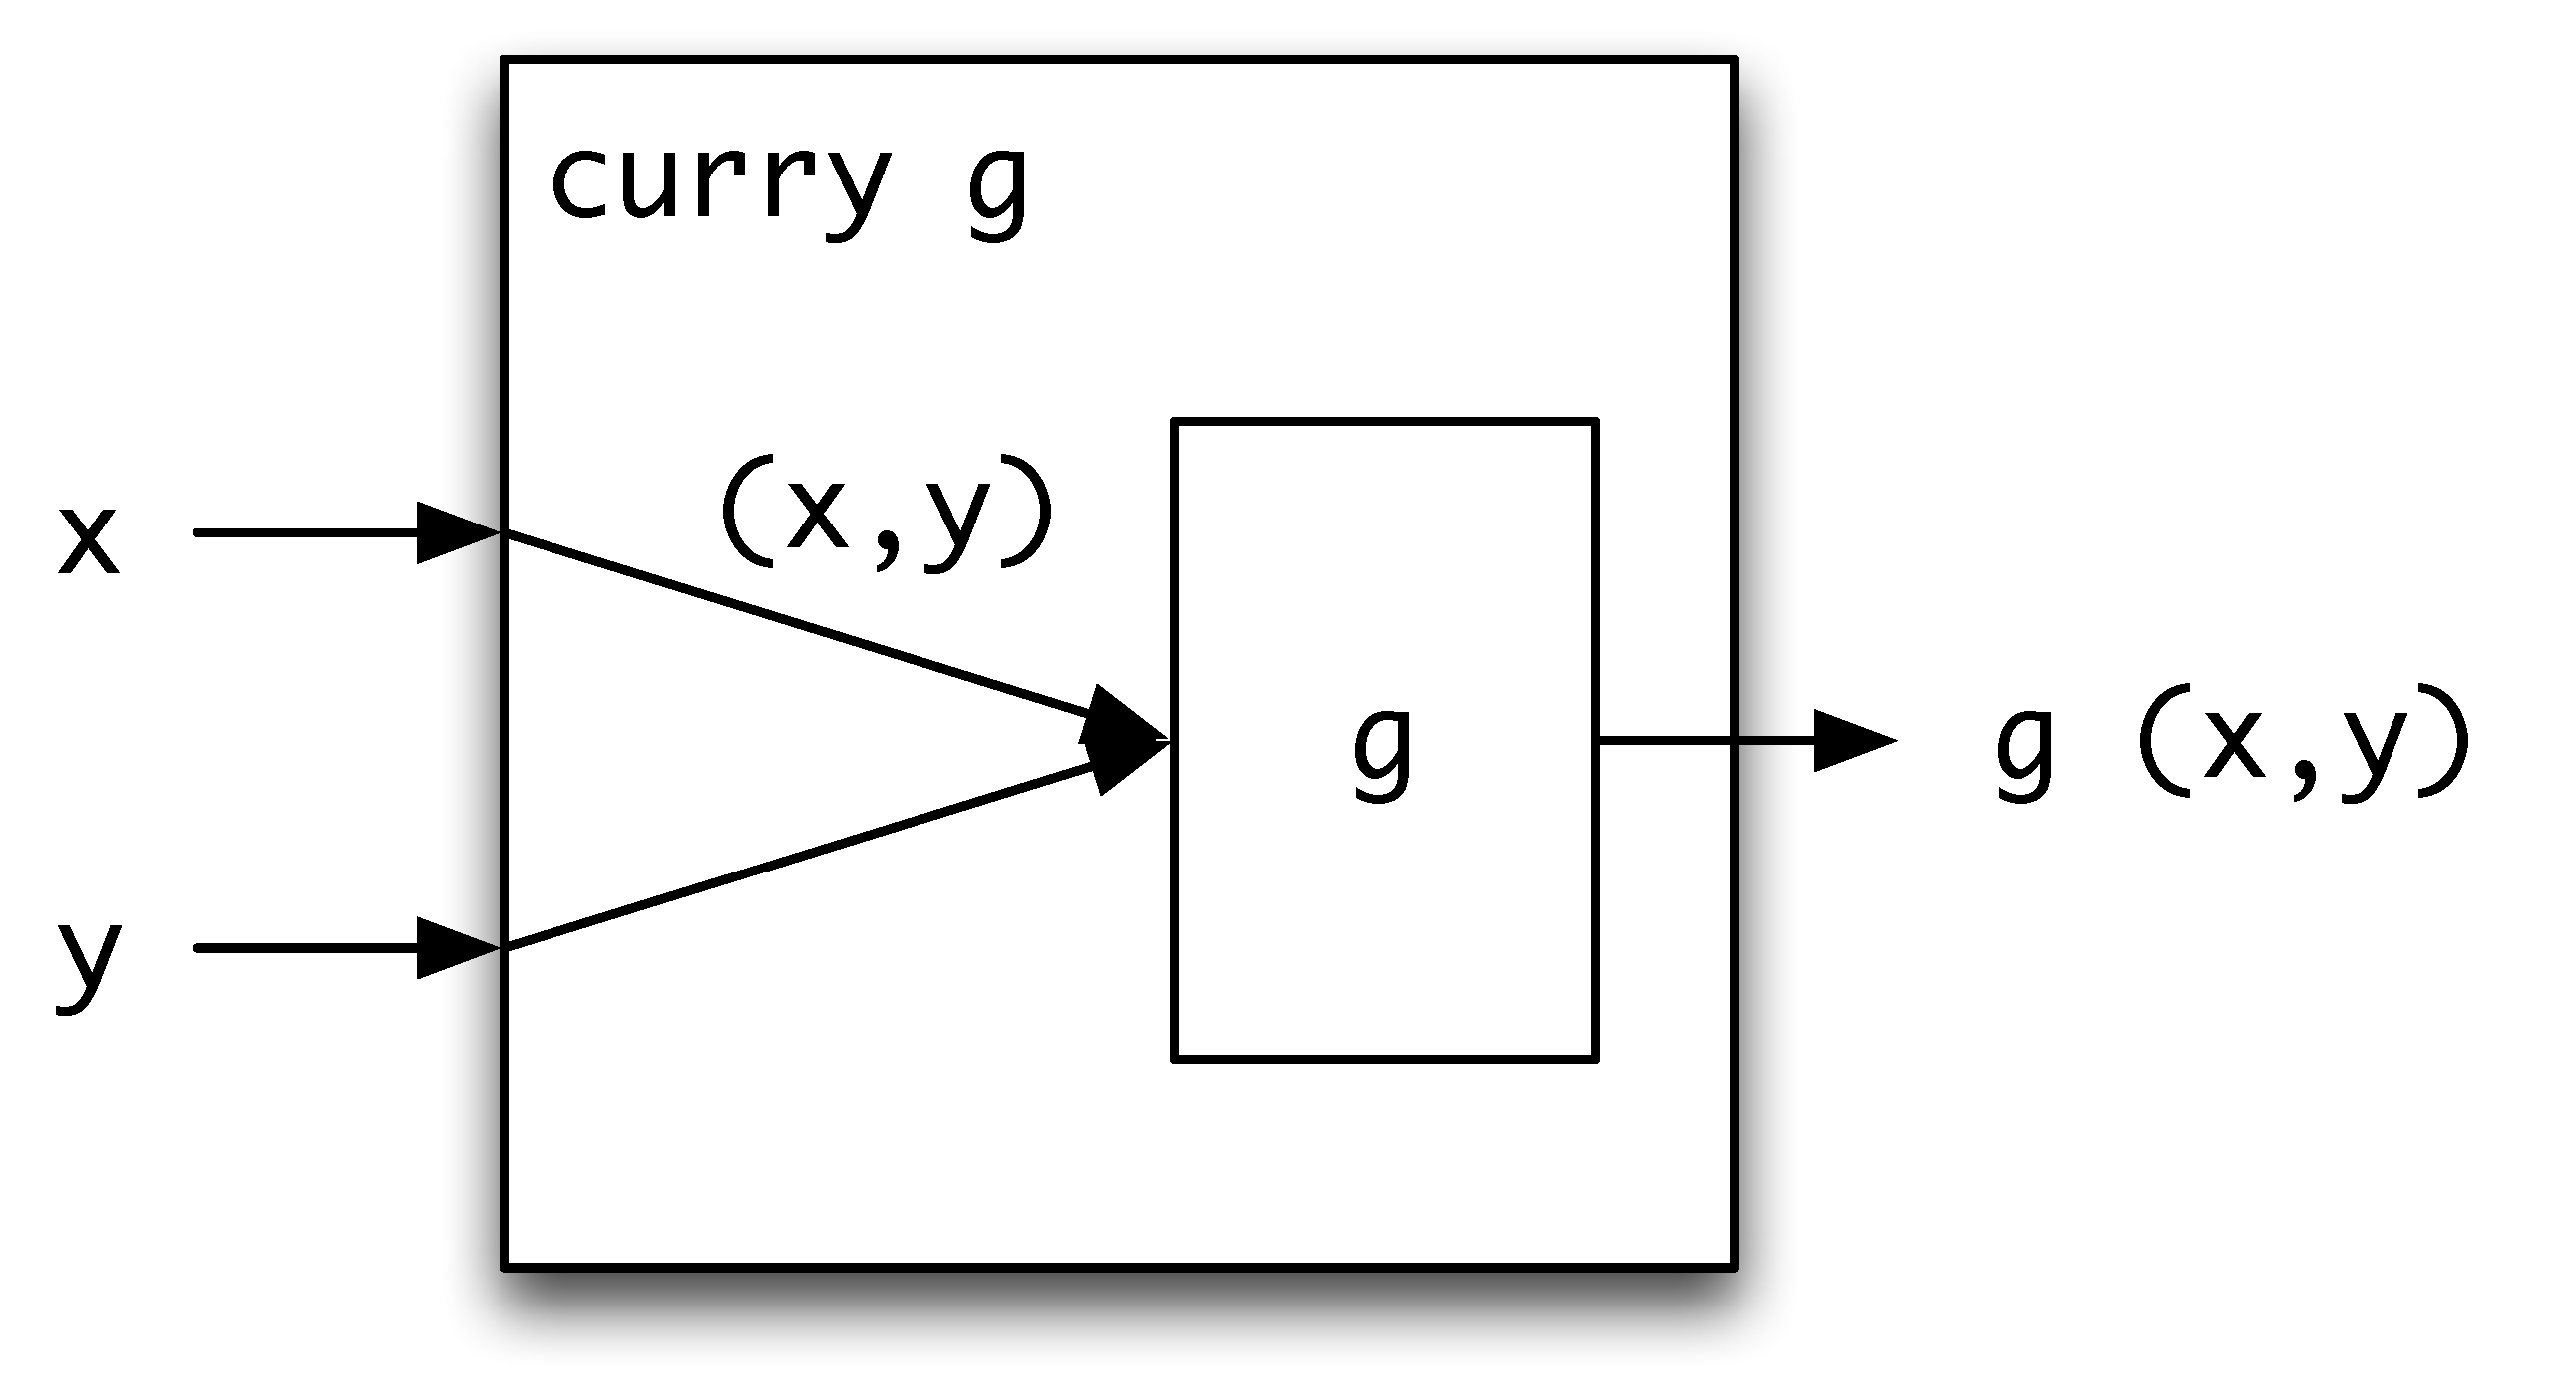
\includegraphics[width=3in]{Pictures/curry.pdf}
\end{center}
This function expects its arguments as a pair, but its curried version,
\texttt{curry g}, will take them separately -- we therefore have to form them into a
pair before applying \texttt{g} to them: 
\begin{alltt}
curry :: ((a,b) -> c) -> (a -> b -> c)\minx{curry}
curry g x y = g (x,y)
\end{alltt}
\texttt{curry multiplyUC} will be exactly the same function as \texttt{multiply}.

Suppose now that \texttt{f} is a curried function, of type 
\texttt{a -> b -> c}. 
\begin{center}
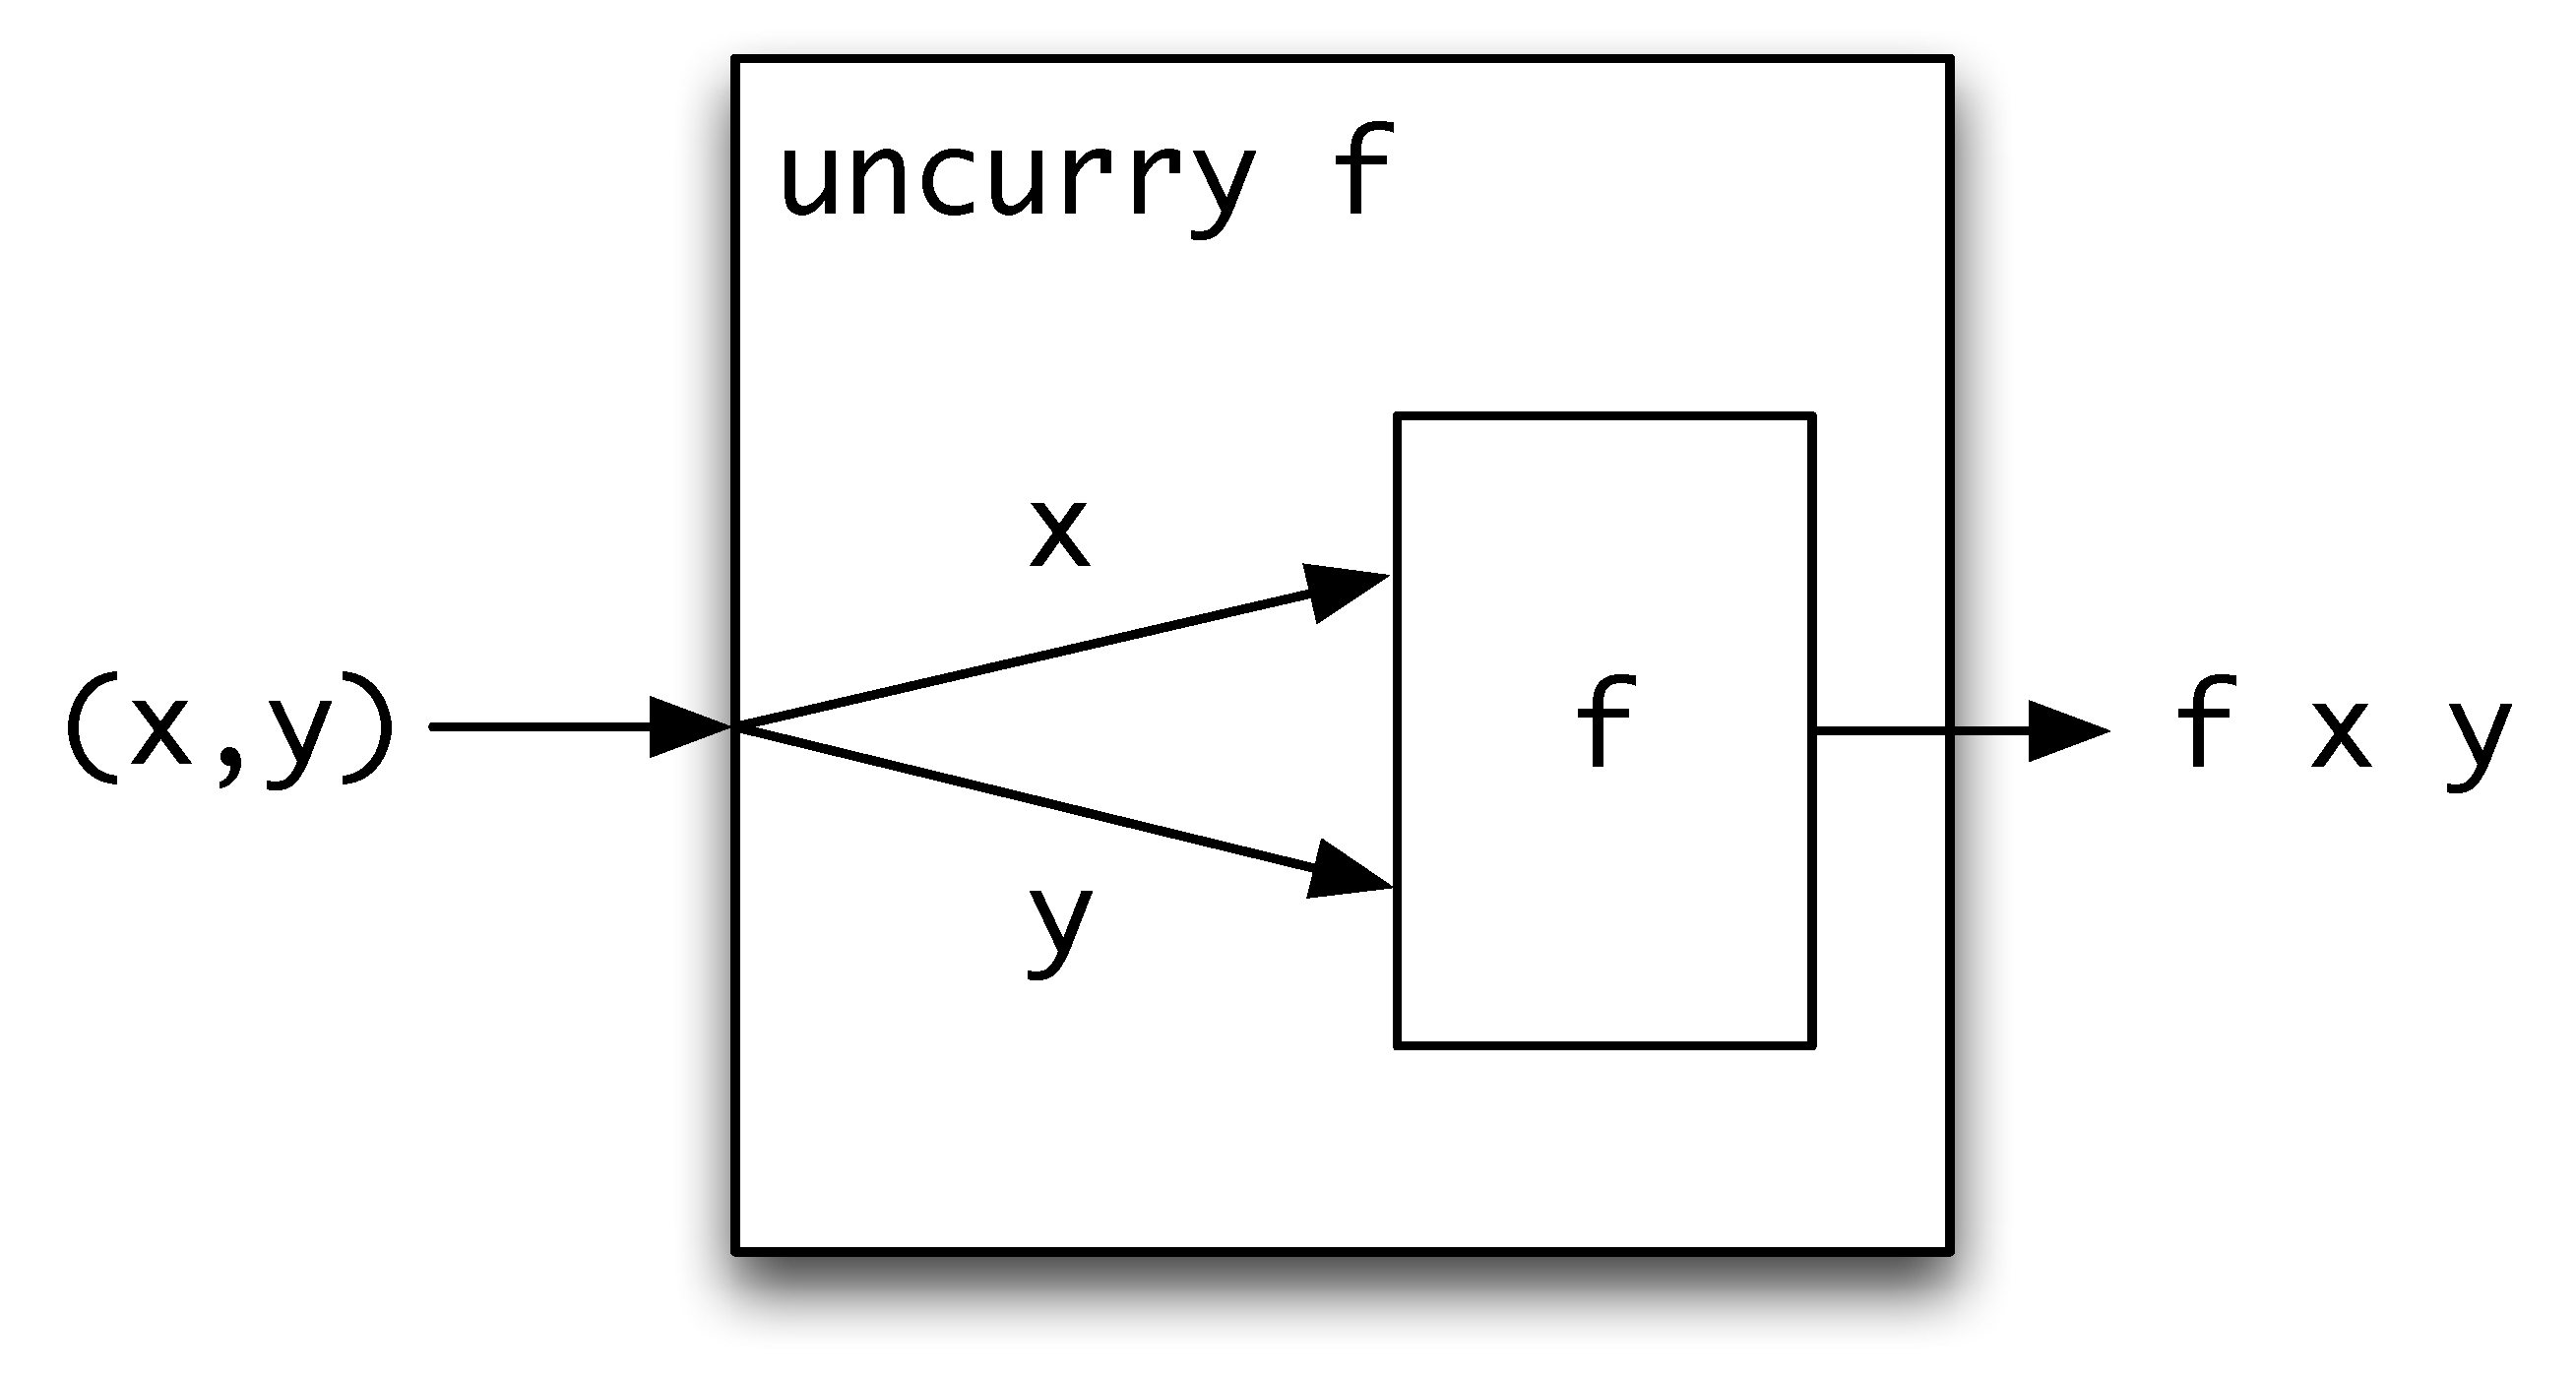
\includegraphics[width=3.0in]{Pictures/uncurry.pdf}
\end{center}
The function \texttt{uncurry f} will expect its
arguments as a pair, and these will have to be separated before
\texttt{f} can be applied to them:
\begin{alltt}
uncurry :: (a -> b -> c) -> ((a,b) -> c)\minx{uncurry}
uncurry f (x,y) = f x y
\end{alltt}
\texttt{uncurry multiply} will be exactly the same function as \texttt{multiplyUC}.
The functions \texttt{curry} and \texttt{uncurry} are inverse to each other.
\index{function!inverse}


A disadvantage of the curried representation of functions is that the inverse of a function like 
\begin{alltt}
unzip ::\ ([a,b]) -> ([a],[b])
\end{alltt}
is not \texttt{zip ::\ [a] -> [b] -> [(a,b)]} but in fact
\begin{alltt}
uncurry zip :: ([a],[b]) -> [(a,b)]
\end{alltt}
(or \texttt{zip'} as we called it earlier in the book) so that statements of properties of these functions, such as
\begin{alltt}
prop_zip xs = uncurry zip (unzip xs) == xs
\end{alltt}
will necessarily involve the uncurried version of the binary function, rather than the curried.

\begin{exercises}

\item
What is the effect of \texttt{uncurry (\$)}? What is its type? Answer a similiar question for \texttt{uncurry (:)}, \texttt{uncurry (.)}.

\item {[Harder]} What are the effects and types of \texttt{uncurry uncurry}, \texttt{curry uncurry}.

\item
Can you state a property relating \texttt{unzip} and \texttt{uncurry zip}, where the latter is the function applied first?

\item
Can you define functions 
\begin{alltt}
curry3 :: ((a,b,c) -> d) -> (a -> b -> c -> d)
uncurry3 :: (a -> b -> c -> d) -> ((a,b,c) -> d)
\end{alltt}
which perform the analogue of \texttt{curry} and \texttt{uncurry} but for three arguments rather than two? Can you use \texttt{curry} and \texttt{uncurry} in these definitions?

\item {[Harder]}
Can you define functions 
\begin{alltt}
curryList :: ([a] -> d) -> (a -> [a] -> d)
uncurryList :: (a -> [a] -> d) -> ([a] -> d)
\end{alltt}
which perform the analogue of \texttt{curry} and \texttt{uncurry} but for a list of  arguments rather than two distinct arguments? Can you use \texttt{curry} and \texttt{uncurry} in these definitions?

\end{exercises}

\index{currying|)}


\section{Defining higher-order functions}
\label{defHOFs}
\index{higher-order function!defining HOFs|(}

This section revises the different ways that we can use to define higher-order functions, and in particular functions that return functions as results. These functions are one of the features of functional programming not shared with most other programming languages that you might be familiar with, and give Haskell particular elegance and power.

\subsection*{Using the operators}

We can use the built-in operators in defining functions directly. We already saw that we could define forward composition in terms of composition,
\begin{alltt}
f >.> g = g.f
\end{alltt}
We also saw this in action in the definition of \texttt{rotate} from the \texttt{Picture} case study:
\begin{alltt}\minx{rotate}
rotate :: Picture -> Picture
rotate = flipV . flipH
\end{alltt}
where again the function is defined directly as the \emph{composition} of two other functions.
The meaning of this definition is just the same as one which has explicit arguments:
\begin{alltt}\minx{rotate}
rotate pic = flipV (flipH pic)
\end{alltt}
but the earlier definition is clearer to read and to
modify; we see \emph{explicitly} that the definition is a composition
of two functions, rather than having to see it as a consequence of the
way the right-hand side is defined in the latter equation.

More importantly, if we state a definition in this form, then we can
apply properties of `\texttt{.}' in analysing how \texttt{rotate}
behaves. This means that in proofs we are able to use properties of composition, as
well as being able to see examples of program transformations which will apply because of the form of composition involved. In general these remarks will apply to all 
higher-order, polymorphic functions, and we see examples of this in Section 
\ref{verifGen} below.


Let's look at some more examples which use composition in their definitions: the 
simplest is this: 
\begin{alltt}
twice f = f.f\hfill (twice.1)\minx{twice}
\end{alltt}
\texttt{f} is a function, and the result is \texttt{f} composed with itself. For
this to work, it needs to have the same input and output type, so we have
\begin{alltt}
twice :: (a -> a) -> (a -> a)
\end{alltt}
This states that \texttt{twice} takes one argument, a function of type 
\texttt{(a -> a)}, and returns a result of the same type. For instance, if \texttt{succ}
is the function to add one to an integer, 
\begin{alltt}
succ :: Integer -> Integer
succ n = n+1
\end{alltt}
then applying \texttt{twice} to it gives the example
\begin{alltt}
(twice succ) 12
\step (succ.succ) 12 \hfill {\rm by} (twice.1)
\step succ (succ 12) \hfill {\rm by definition of } .
\step 14
\end{alltt}
We can generalize \texttt{twice} so that we pass a parameter giving the number
of times the functional argument is to be composed with itself
\begin{alltt}
iter :: Integer -> (a -> a) -> (a -> a)\minx{iter}

iter n f 
  | n>0         = f . iter (n-1) f\hfill(iter.1)
  | otherwise   = id\hfill(iter.2)
\end{alltt}
This is a standard primitive recursion over the integer argument; in the
positive case we take the composition of \texttt{f} with itself
\texttt{n-1} times and compose once more with \texttt{f}. In the zero case
we apply \texttt{f} no times, so the result is a function which returns its argument unchanged, namely \texttt{id}. 

As an example of using \texttt{iter}, we can define \texttt{\superscr{2}{n}} as \texttt{iter n double
1}, if \texttt{double} doubles its argument. 


\begin{exercises}

\item
Give calculations of
\begin{alltt}
{\hskip1pc}iter 3 double 1
(comp2 succ (*)) 3 4
comp2 sq add 3 4
\end{alltt}

\item
What is the type and effect of the function
\begin{alltt}
\bs{n} -> iter n succ
\end{alltt}

\item 
Give an alternative ``constructive'' definition of \texttt{iter} which creates the list of \texttt{n} copies of \texttt{f}
\begin{alltt}
[f,f,...,f]
\end{alltt} and then composes these functions by folding in the
operator `\texttt{.}' to give 
\begin{alltt}
f . f . \ldots\ . f
\end{alltt}



\end{exercises}

\subsection*{Using local definitions}

Local definitions allow us to define functions as a subsidiary part of a function definition. We looked earlier at the example of 
\begin{alltt}
addNum :: Integer -> Integer -> Integer
\end{alltt}
We can use a local definition to give the result, either using a \texttt{where}
\begin{alltt}
addNum n = addN
		   where
		   addN m = n+m
\end{alltt}
or a \texttt{let}
\begin{alltt}
addNum n = let 
             addN m = n+m
           in
             addN
\end{alltt}
This gives us a way of defining results which are functions by locally defining that function and returning it as the result; it has the advantage of not requiring any more advanced machinery, but the disadvantage of introducing a named definition of \texttt{addN} which is extraneous to the actual result. 		   

\subsection*{Lambda abstractions}

Let's try to define a function that takes a binary function as argument, and which returns a binary function that takes its arguments in the opposite order; let's call it \texttt{flip}:
\begin{alltt}
flip :: (a -> b -> c) -> (b -> a -> c)\minx{flip}
\end{alltt}
We can use a lambda abstraction to give the result:
\begin{alltt}
flip f = \bs{}x y -> f y x\hfill(flip.1)
\end{alltt}
This makes clear that a function like
\texttt{flip map} takes as its first argument the list and as its second
the function to be mapped; it can then be partially applied to its first argument, having
the effect of applying \texttt{map} to its second only. This allows us to do a partial application to the second argument of a two argument function.

\subsection*{Partial application}

Partial applications give us a particularly direct way of defining some higher order functions. Taking the example we have just looked at, we can instead say
\begin{alltt}\minx{flip}
flip f x y = f y x
\end{alltt}
If we apply \texttt{flip} to one argument, we have a function which behaves just as described in \texttt{(flip.1)}. Similarly, the behaviour of 
\begin{alltt}
addNum n = addN
		   where
		   addN m = n+m
\end{alltt}
is given by the simple definition
\begin{alltt}
addNum n m = n+m
\end{alltt}
partially applied to \texttt{n}.

\beware{Constructors are functions too}{
Datatype constructors are functions, and so they can be partially applied, passed as arguments to functions or indeed returned as results. To give just one example, this expression creates a list of \texttt{People} from lists of names and ages:
\begin{alltt}
zipWith Person ["Geraint","Bob"] [45,67]
\end{alltt}
}

\begin{figure}[t]\index{point-free programming}
\beware{Point-free programming}{
Some function-level, or `point-free', definitions express what the function does with real clarity: writing\label{pointfree}
\texttt{
flipV = map reverse\ }
precisely describes how to flip a picture in a vertical mirror. However, it is possible to take this approach too far, and write definitions which it's very hard to understood. For instance, what does this function do:
\begin{alltt}
puzzle = (.) (.)
\end{alltt}
Reading the definition tells us that it is the composition operator partially applied to itself, but still it's not clear what the function will do. How can we work out what it does? The best way is to apply it to some arguments and see what it does:
\begin{alltt}
(.) (.) x \step{}(.).x
\end{alltt}
so
\begin{alltt}
(.) (.) x y \step{}((.).x) y \step{}(.) (x y)
\end{alltt}
Applying to a third argument gives
\begin{alltt}
(.) (.) x y z \step \ldots\ \step{}(.) (x y) z \step{}(x y) . z
\end{alltt}
and finally 
\begin{alltt}
(.) (.) x y z w \step \ldots\ \step{}((x y) . z) w \step{}(x y) (z w)
\end{alltt}
giving us the much more informative explanation:
\begin{alltt}
puzzle x y z w = (x y) (z w)
\end{alltt}
Finally, we use to get GHCi to give its type, like this \texttt{:type (.)(.)} and get
\begin{alltt}
(.)(.) :: (a1 -> b -> c) -> a1 -> (a -> b) -> a -> c
\end{alltt}
So there we are \ldots\ To be fair, once we understand what \texttt{puzzle} does, it can be useful to have the original definition which explicitly uses the composition operator, because then any general laws that we discover for \texttt{(.)} will apply to \texttt{puzzle} too.
}
\end{figure}




\subsection*{Examples}

We conclude this section by exploring how partial applications and operator sections can be
used to simplify and shorten definitions in a number of other examples. 
Often it is possible to avoid
giving an explicit function definition if we can use a partial application to
return a function. Revisiting the examples of Chapter \ref{defFunLists} we see that
to double all the elements in a list we can write
\begin{alltt}
doubleAll :: [Int] -> [Int]
doubleAll = map (*2)\minx{doubleAll}
\end{alltt}
using an operator section \texttt{(*2)} to replace the \texttt{double} function,
and giving the function definition directly by partially applying \texttt{map}.

To filter out the even elements in a numerical list, we have to check whether
the remainder on dividing by two is equal to zero. As a function we can write
\begin{alltt}
(==0).(`mod` 2)
\end{alltt}
This is the composition of two operator sections: first find the remainder on dividing by
two,
then check if it is equal to zero. (Why can we not write \texttt{(`mod` 2 ==
0)}?) The filtering function can then be written
\begin{alltt}\minx{getEvens}
getEvens :: [Int] -> [Int]
getEvens = filter ((==0).(`mod` 2))
\end{alltt}
Our final example comes from the list splitting study. We defined
\begin{alltt}
getWord xs 
  = getUntil p xs\minx{getWord}
    where 
    p x = elem x whitespace
\end{alltt}
The local definition is not now needed, as we can define the function \texttt{p}
by an operator section:
\begin{alltt}\minx{getWord}
getWord xs = getUntil (`elem` whitespace) xs
\end{alltt}
Note the way that we partially apply a
function to its {\em second\/} argument, by forming an operator section. This
works because
\begin{alltt}
(`elem` whitespace) x
= x `elem` whitespace
= elem x whitespace
\end{alltt}
as required.

Finally, the 
function \texttt{getWord} can itself be given a direct definition,
by partial application thus
\begin{alltt}
getWord = getUntil (`elem` whitespace)
\end{alltt}
This definition reads like an informal explanation -- to get a word, get
characters until a whitespace character is found.
 


\begin{exercises}

\item
Using partial application re-define the function 
\begin{alltt}
mapFuns :: [a->b] -> a -> [b]
\end{alltt}
first defined in Section \ref{exprFuns}.


\item
{[Harder]} Define a function
\begin{alltt}
{\hskip1pc}slope :: (Float -> Float) -> (Float -> Float)
\end{alltt}
which takes a function \texttt{f} as argument, and returns (an approximation to)
its derivative \texttt{f'} as result.


\item
{[Harder]} Define a function
\begin{alltt}
{\hskip1pc}integrate :: (Float -> Float) -> (Float -> Float -> Float)
\end{alltt}
which takes a function \texttt{f} as argument, and returns (an approximation to)
the two argument function which gives the area under its graph between two end
points as its result.

\end{exercises}
  
\index{higher-order function!defining HOFs|)}




\markright{Verification and general functions}

\section[Verification and general functions]{Verification and
general functions}
\index{proof!higher-order functions|(}
\index{higher-order function!proofs}
\label{verifGen}
\markright{Verification and general functions}

Verification can take on a different character when we look at higher-order
polymorphic functions. We can start to prove equalities between functions,
rather than between values of functions, and we shall also see that we are able
to prove theorems which resemble their subjects in being general and reusable,
and so applicable in many contexts.

\subsection*{Function-level verification}
\index{proof!function level}

We claimed in Section \ref{defHOFs} that the function \texttt{iter} is
a generalization of \texttt{twice}, since
\begin{alltt}\minx{iter}\minx{twice}
iter 2 f
  = f . iter 1 f\hfill {\rm by} (iter.1)
  = f . (f . iter 0 f)\hfill {\rm by} (iter.1)
  = f . (f . id)\hfill {\rm by} (iter.2)
  = f . f\hfill {\rm by} (compId)
  = twice f\hfill {\rm by} (twice.1)
\end{alltt}
In proving this we have used the equality between two functions
\begin{alltt}
f . id = f \hfill \texttt{(compId)}
\end{alltt}
How is this proved? We examine how each side behaves on an arbitrary argument
\texttt{x}
\begin{alltt}
(f . id) x
  = f (id x)
  = f x
\end{alltt}
so that for any argument \texttt{x} the two functions have the same
behaviour. As black boxes, they are therefore the same. 
As what interests us here is their behaviour,
we say that they are equal. We call this `black-box' concept of equality 
\textbf{extensional}.

\begin{definition}{{\sffamily Principle of extensionality:}
\index{extensionality principle}
\medskip

\noindent
Two functions \texttt{f} and \texttt{g} are equal if they have the same value at
every argument.}
\end{definition}

\noindent
This is called extensionality in contrast to the idea of\index{intensionality} 
\textbf{intensionality} in which we say two functions are the same only if they have
the same definitions -- we no longer think of them as black boxes; we
are allowed to look inside them to see how the mechanisms work, as it were. If
we are interested in the results of our programs, all that matters are the
values given by functions, not how they are arrived at. We therefore use
extensionality when we are reasoning about function behaviour in Haskell. If
we are interested in \textbf{efficiency} or other performance aspects of
programs, then the way in which a result is found {\em will\/} be significant,
however. This is discussed further in Chapter \ref{behaviour}.

\begin{exercises}


\item
Using the principle of extensionality, show that function composition 
is associative: that is, for all \texttt{f}, {\mi
g} and \texttt{h},
\begin{alltt}
f . (g . h) = (f . g) . h
\end{alltt}\index{function composition!associative}

\item
Show that for all \texttt{f},
\begin{alltt}
id . f = f
\end{alltt}

\item
Show that the function \texttt{flip} defined in Section \ref{curry} satisfies
\begin{alltt}
flip . flip = id
\end{alltt}
Hint: to show this, you might want to prove that for any \texttt{f},
\begin{alltt}
flip (flip f) = f
\end{alltt}

\item
Two functions \texttt{f} and \texttt{g} are \textbf{inverses} if it can be shown that
\index{function!inverse}
\begin{alltt}
f . g = id              g . f = id
\end{alltt}
Prove that the functions \texttt{curry} and \texttt{uncurry} of Section \ref{curry}
are inverses. Can you think of other pairs of inverse functions?

\item
Using induction, prove that for all natural numbers \texttt{n},
\begin{alltt}
iter n id = id
\end{alltt}

\item
A function \texttt{f} is called \textbf{idempotent} if\index{idempotence} 
\begin{alltt}
f . f = f
\end{alltt}
Show that the functions \texttt{abs} and \texttt{signum} are idempotent. Can you
think of any other idempotent functions?
\end{exercises}

\subsection*{Higher-level proofs}
\index{proof!higher-level}

Our verification thus far has concentrated on first-order, monomorphic
functions. Just as \texttt{map}, \texttt{filter} and \texttt{fold} generalize
patterns of definition, we shall find that proofs about these functions
generalize results we have seen already. To give some examples, it is
not hard to prove that
\begin{alltt}
doubleAll (xs++ys) = doubleAll xs ++ doubleAll ys\minx{doubleAll}
\end{alltt}
holds for all finite lists \texttt{xs} and \texttt{ys}.
When \texttt{doubleAll} is defined as \texttt{map (*2)} it becomes clear that we have an
example of a general result,
\begin{alltt}\index{map@\texttt{map}}
map f (xs++ys) = map f xs ++ map f ys\index{map@\texttt{map}}\hfill(map++)
\end{alltt}
which is valid for {\em any\/} function \texttt{f}.
We also claimed in an earlier exercise that
\begin{alltt}
sum (xs++ys) = sum xs + sum ys\hfill (sum.3)
\end{alltt}
for all finite lists \texttt{xs}, \texttt{ys}. The function \texttt{sum} is given by
folding in \texttt{(+)}, 
\begin{alltt}\minx{sum}\index{foldr@\texttt{foldr}}
sum = foldr (+) 0
\end{alltt}
and we have, generally,
if \texttt{f} is associative, and \texttt{st} is an identity for \texttt{f}, that is,
\begin{alltt}\label{assocId}
x `f` (y `f` z) = (x `f` y) `f` z
x `f` st = x = st `f` x
\end{alltt}
for all \texttt{x}, \texttt{y}, \texttt{z}
then the equation 
\begin{alltt}
foldr f st (xs++ys) = f (foldr f st xs) (foldr f st ys)\hfill (foldr.3)\index{foldr@\texttt{foldr}}
\end{alltt}
holds for all finite \texttt{xs} and \texttt{ys}. Obviously \texttt{(+)} is associative and has
\texttt{0} as an identity, and so \texttt{(sum.3)} is a special case of
\texttt{(foldr.3)}.
Now we give three proofs of examples in the same vein.

\subsection*{\texttt{map} and composition}
\index{function composition}\index{map@\texttt{map}}

A first example concerns \texttt{map} and composition. Recall the definitions
\begin{alltt}
map f []     = [] \hfill (map.1)
map f (x:xs) = f x : map f xs\hfill (map.2)
(f . g) x    = f (g x)\hfill (comp.1)
\end{alltt}
It is not hard to see that we should be able to prove that
\begin{alltt}
map (f . g) xs = (map f . map g) xs \hfill (map.3)
\end{alltt}
holds for every
finite list \texttt{xs}. 
\begin{center}
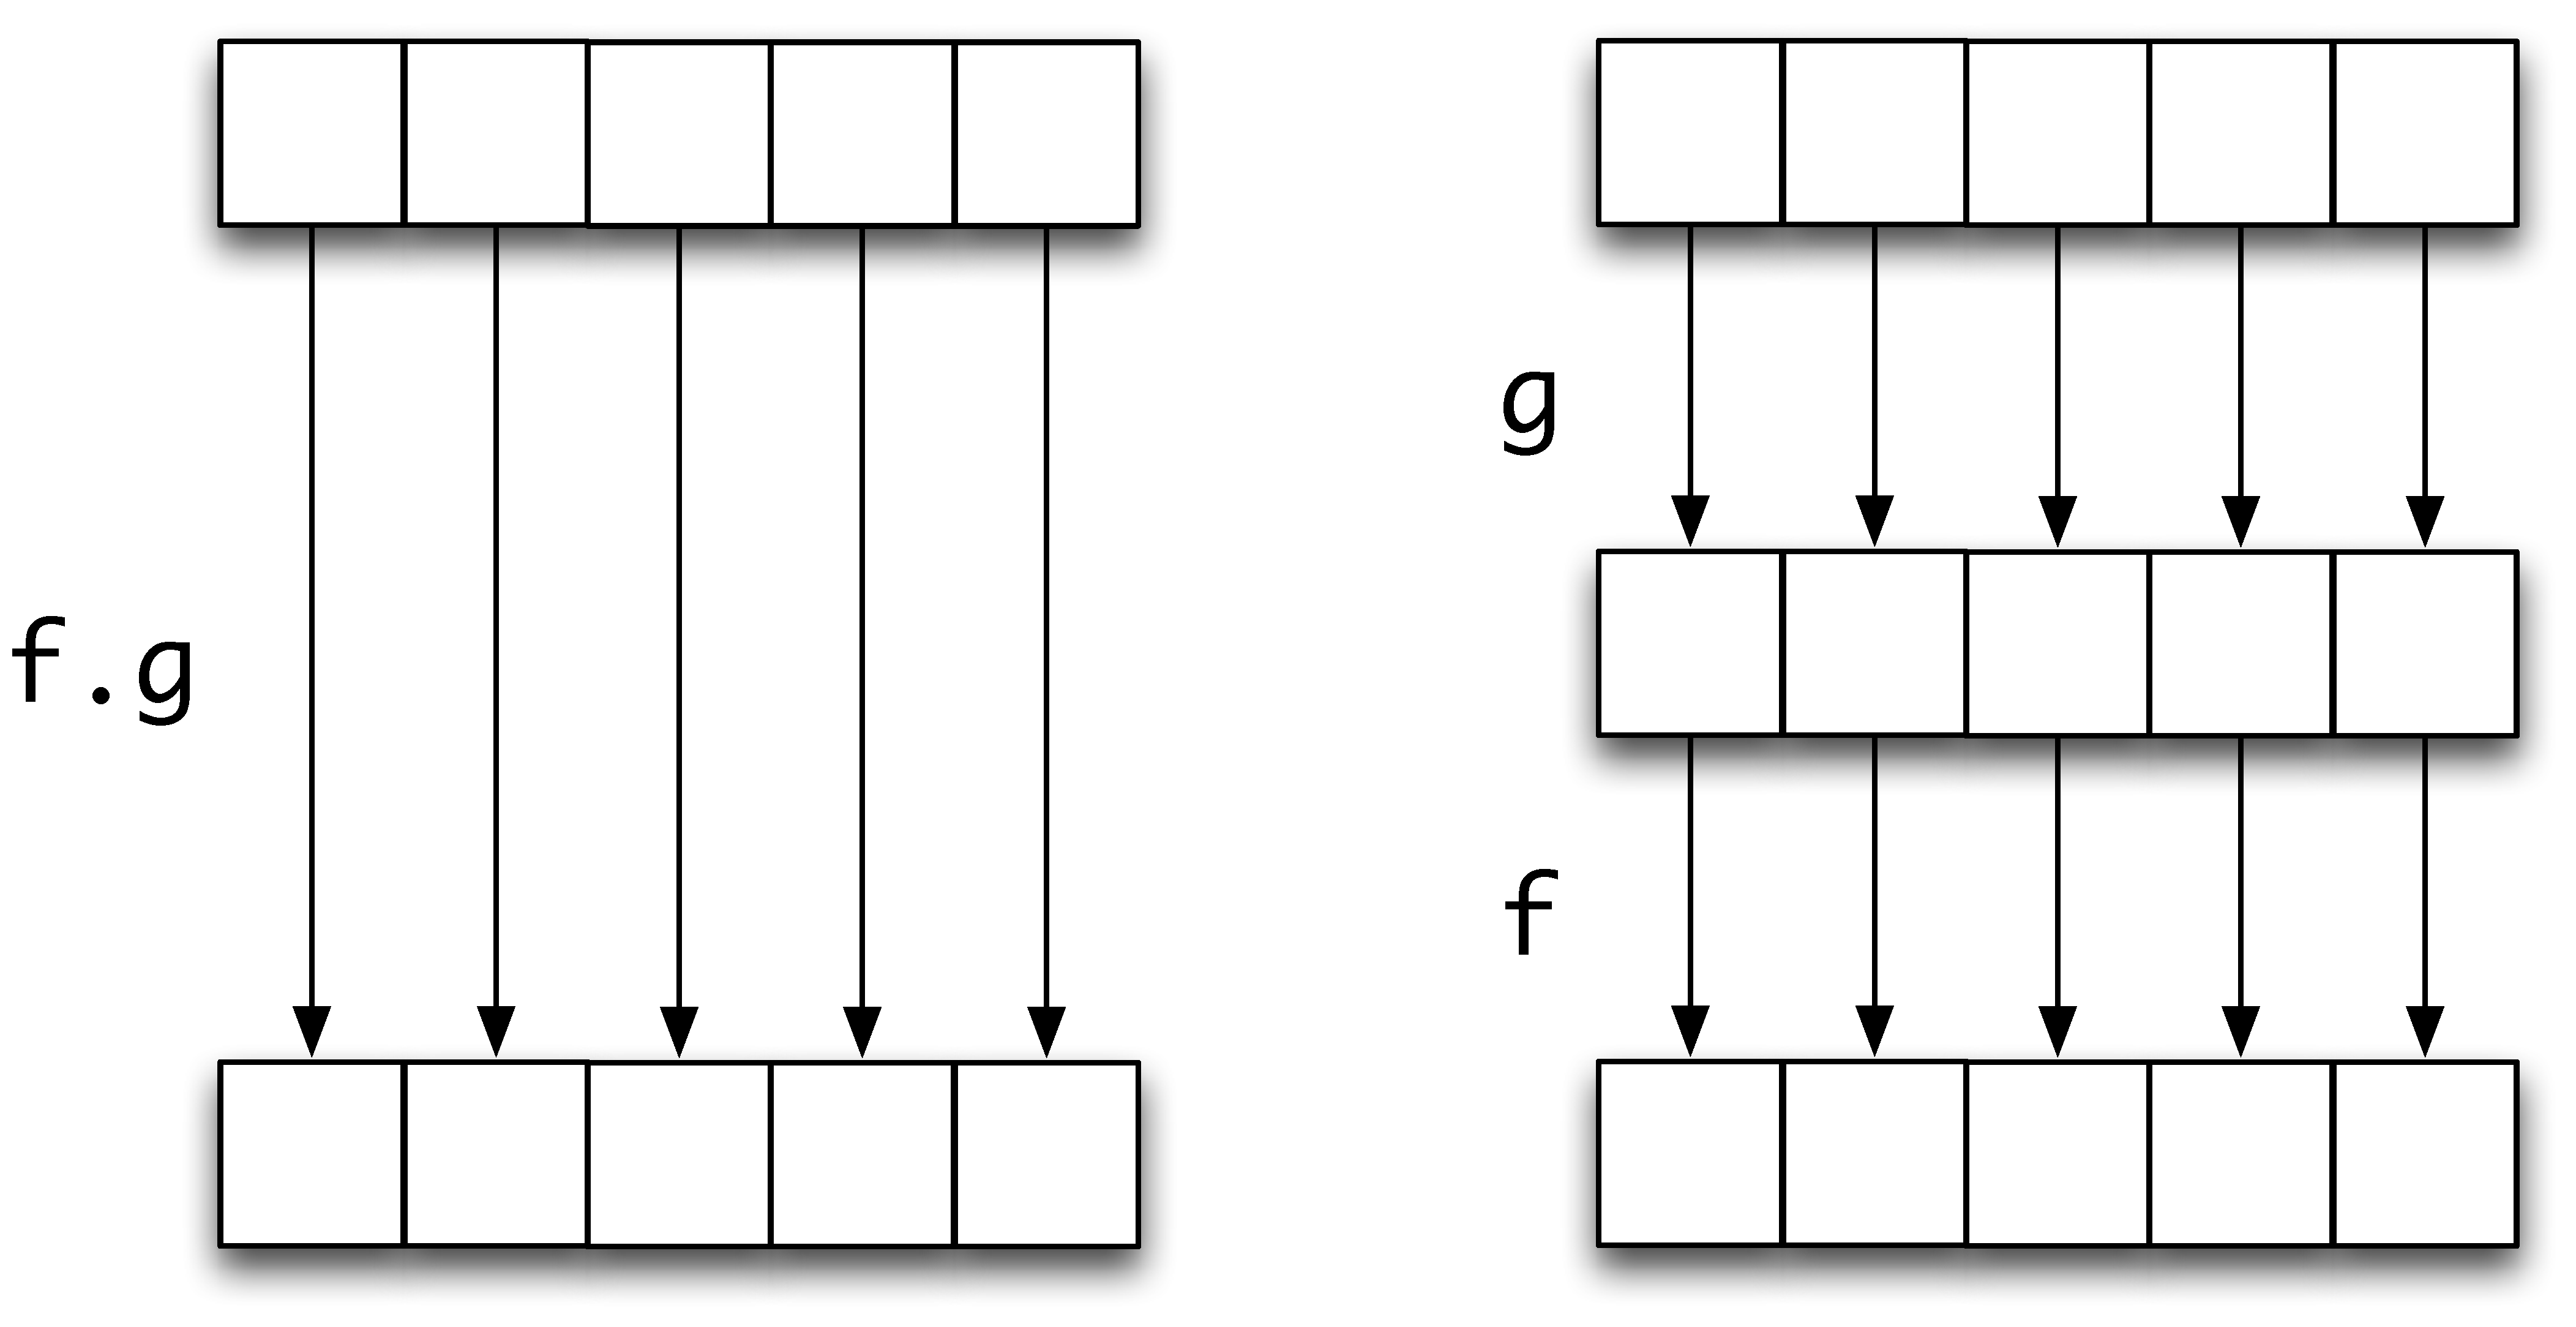
\includegraphics[width=3.5in]{Pictures/mapComp.pdf}
\end{center}
Applying 
\texttt{(f .\ g)} to every member of a list should be the same as applying \texttt{g} to
every member of the list and then applying \texttt{f} to every member of the result. It is proved
just as easily, by structural induction\index{structural induction}. 
The \texttt{(base)} case requires the identity
to be proved for the empty list.
\begin{alltt}
map (f . g) [] = [] \hfill {\rm by} (map.1)
\bl
(map f . map g) [] 
  = map f (map g []) \hfill {\rm by} (comp.1)
  = map f [] \hfill {\rm by} (map.1)
  = [] \hfill {\rm by} (map.1)
\end{alltt}
Assuming that 
\begin{alltt}
map (f .\ g) xs = (map f .\ map g) xs\hfill(hyp)
\end{alltt} is true,
it is now necessary to prove that 
\begin{alltt}
map (f . g) (x:xs) = (map f . map g) (x:xs)\hfill(ind)
\end{alltt}
Again, it is enough to analyse each side of the equation.
\begin{alltt}
map (f . g) (x:xs) 
  = (f . g) x : map (f . g) xs \hfill {\rm by} (map.2)
  = f (g x) : map (f . g) xs \hfill {\rm by} (comp.1)
\bl
(map f . map g) (x:xs) 
  = map f (map g (x:xs)) \hfill {\rm by} (comp.1)
  = map f (g x : map g xs) \hfill {\rm by} (map.2)
  = f (g x) : map f (map g xs) \hfill {\rm by} (map.2)
  = f (g x) : (map f . map g) xs \hfill {\rm by} (comp.1)
\end{alltt}
The induction hypothesis is exactly what is needed to prove the two sides
equal,
completing the proof of the induction step and the proof itself. \blackbox

Each Haskell list type, besides containing finite lists,
also contains infinite and partial lists. In Chapter \ref{lazy}
these will be explained and it will be shown that 
\texttt{(map.3)} is true for {\em all\/} lists \texttt{xs}, and therefore that the functional
equation
\begin{alltt}
map (f . g) = (map f) . (map g)
\end{alltt}
holds in general.

\subsection*{\texttt{map} and \texttt{filter}}
\index{map@\texttt{map}}\index{filter@\texttt{filter}}


The proof above showed how properties of functional programs could be proved
from the definitions of the functions in a straightforward way. The properties
can state how the program behaves -- that a sorting function returns an ordered
list, for instance -- or can relate one program to another. This latter idea
underlies \textbf{program transformation}\index{program transformation}
for functional languages. This section
introduces an example 
called \textbf{filter promotion} which is one of the most
useful of the basic functional transformations.
\begin{alltt}
filter p . map f = map f . filter (p . f)\hfill(filter/map)\label{filterMap}
\end{alltt}
The equation says that a \texttt{map} followed by a \texttt{filter} can be replaced
by a \texttt{filter} followed by a \texttt{map}. The right-hand side is potentially
more efficient than the left, since the \texttt{map} operation will there be
applied to a shorter list, consisting of just those elements with the property
\texttt{(p .\ f)}.
An example is given by the function first defined in Section \ref{opsecs}.
\begin{alltt}
filter (0<) . map (+1)
\end{alltt}
Instead of mapping first, the function can be replaced by
\begin{alltt}
map (+1) . filter ((0<) . (+1))
 = map (+1) . filter (0<=)
\end{alltt}
and it is clear that here the transformed version is more efficient,
since the test \texttt{(0<=)} is no more
costly than \texttt{(0<)}.
The proof that
\begin{alltt}
(filter p . map f) xs = (map f . filter (p . f)) xs
\end{alltt}
for finite lists \texttt{xs} is by structural induction.\index{structural
induction}
First we reiterate the definitions of \texttt{map}, \texttt{filter} and {\mi
composition}.
\begin{alltt}
map f []        = [] \hfill (map.1)
map f (x:xs)    = f x : map f xs\hfill (map.2)
\bl
filter p []     = []\hfill (filter.1)
filter p (x:xs) 
  | p x         = x : filter p xs\hfill (filter.2)
  | otherwise   =     filter p xs\hfill (filter.3)
\bl
(f . g) x       = f (g x)\hfill (comp.1)
\end{alltt}
The base case consists of a proof of 
\begin{alltt}
(filter p . map f) [] = (map f . filter (p . f)) [] \hfill (base)
\end{alltt}
This is true since
\begin{alltt}
(filter p . map f) []
  = filter p (map f []) \hfill {\rm by} (comp.1)
  = filter p [] \hfill {\rm by} (map.1)
  = [] \hfill {\rm by} (filter.1)
\end{alltt}
and
\begin{alltt}
(map f . filter (p . f)) []
  = map f (filter (p . f) [])  \hfill {\rm by} (comp.1)
  = map f []  \hfill {\rm by} (filter.1)
  = []  \hfill {\rm by} (map.1)
\end{alltt}
In the induction step, a proof of 
\begin{alltt}
(filter p . map f) (x:xs) = (map f . filter (p . f)) (x:xs) \hfill (ind)
\end{alltt}
is required, using the induction hypothesis
\begin{alltt}
(filter p . map f) xs = (map f . filter (p . f)) xs \hfill (hyp)
\end{alltt}
The proof begins with an analysis of the left-hand side of \texttt{(ind)}.
\begin{alltt}
(filter p . map f) (x:xs)
  = filter p (map f (x:xs))  \hfill {\rm by} (comp.1)
  = filter p (f x : map f xs) \hfill {\rm by} (map.2)
\end{alltt}
There are two\footnote{
We should also think about what happens when {\smtt p (f x)} is undefined; in
this case both sides will be undefined, and so equal.}
cases\index{proof!by cases} to consider:
whether \texttt{p (f x)} is \texttt{True} or \texttt{False}. Taking the case
where  \texttt{p (f x)} is \texttt{True}, we continue to examine the left-hand
side of \texttt{(ind)}, giving
\begin{alltt}
  = f x : filter p (map f xs)  \hfill {\rm by} (filter.2)
  = f x : (filter p . map f) xs \hfill {\rm by} (comp.1)
  = f x : (map f . filter (p . f)) xs \hfill {\rm by} (hyp)
\end{alltt}
Now we look at the right-hand side of \texttt{(ind)}, also assuming 
that \texttt{p (f x)} is \texttt{True}:
\begin{alltt}
(map f . filter (p . f)) (x:xs) 
  = map f (filter (p . f) (x:xs))\hfill {\rm by} (comp.1) 
  = map f (x: (filter (p . f) xs))\hfill {\rm by} (filter.2) 
  = f x : map f (filter (p . f) xs)\hfill {\rm by} (map.2)
  = f x : (map f . filter (p . f)) xs \hfill {\rm by} (comp.1)
\end{alltt}
which shows that \texttt{(ind)} holds in the case that \texttt{p (f
x)} is \texttt{True}.

A similar chain of reasoning gives the same result in the case where
\texttt{p (f x)} is \texttt{False}. This establishes \texttt{(ind)} assuming \texttt{(hyp)}, and so
together with \texttt{(base)} completes the proof of the filter promotion
transformation in the case of finite lists; it holds, in fact, for all
lists. \blackbox

\begin{figure}[t]\index{QuickCheck!and higher-order functions}\index{higher-order function!QuickCheck}
\beware{QuickCheck and higher-order functions}
{\label{QChofs}We've already seen that QuickCheck is a very good way of checking whether particular properties hold for functions that we define. QuickCheck works by generating random test  data and checking whether properties hold at these values. While generating data is not entirely straightforward for structured types like lists and algebraic types, it can be done. Generating random functions is more difficult, and isn't supported ``out of the box'' by QuickCheck: for it to work we need to be able to ``show'' functions. We examine how to do this, and so how to use QuickCheck to test properties involving higher-order functions, in Chapter \ref{dsls}. In the meantime we look at how to check properties for given functions and randomly-generated lists.

\medskip
Let's take the example of the property for \texttt{map} and \texttt{filter}, \texttt{(filter/map)} introduced on page \pageref{filterMap}:
\begin{alltt}
prop_mf p f = 

\ \ \ \ \bs{}xs -> (filter p . map f) xs == (map f . filter (p . f)) xs
\end{alltt}
We can check this for specific values of \texttt{p} and \texttt{f} like this
\begin{alltt}
\textsl{Prompt>} quickCheck (prop_mf (>0) (\bs{}x -> x*x))

\textsl{+++ OK, passed 100 tests.}

\textsl{Prompt>} quickCheck (prop_mf (>=0) (\bs{}x -> x*x*x))

\textsl{+++ OK, passed 100 tests.}
\end{alltt}
where for each instance of \texttt{p} and \texttt{f} the property is tested for 100 randomly generated values.
}\end{figure}


\subsection*{\texttt{map}, \texttt{reverse} and the \texttt{Picture} case study}
\index{map@\texttt{map}}\minx{reverse}\index{pictures}

When we introduced the \texttt{Picture} case study
in Chapter \ref{intro} we claimed that we could prove that 
\texttt{flipV} and \texttt{flipH}
can be applied in either order to give the same result. Our
implementation defines them thus
\begin{alltt}\minx{flipH}\minx{flipV}
flipH = reverse
flipV = map reverse
\end{alltt}
and we can see informally that 
\begin{itemize}
\item
\texttt{reverse} affects the order of the elements, while leaving the
elements unchanged;
\item 
\texttt{map reverse} affects each of the elements, while keeping their
order the same.
\end{itemize}
The second observation is a consequence of the function being a
\texttt{map}, and so we make the more general claim that for all finite lists \texttt{xs} and all
functions \texttt{f},
\begin{alltt}
map f (reverse xs) = reverse (map f xs)\hfill(map/reverse)
\end{alltt}
This has the consequence that
\begin{alltt}
flipV (flipH xs) = flipH (flipV xs)
\end{alltt}
if we replace \texttt{f} in \texttt{(map/reverse)}
by \texttt{reverse}. We will see in Chapter \ref{lazy} that we can
establish
\texttt{(map/reverse)}
for all lists \texttt{xs} and so conclude that the functional equations
hold:
\begin{alltt}
map f . reverse = reverse . map f
flipV . flipH   = flipH . flipV
\end{alltt}
We now prove \texttt{(map/reverse)}
by induction over \texttt{xs}.

We have seen the definition of \texttt{map} in the previous examples;
\texttt{reverse} is defined thus.
\begin{alltt}
reverse []     = []\hfill(reverse.1)
reverse (z:zs) = reverse zs ++ [z]\hfill(reverse.2)
\end{alltt}

\subparagraph{Statement} We first have to prove the base case:
\begin{alltt}
map f (reverse []) = reverse (map f [])\hfill(base)
\end{alltt}
and then we need to prove the induction step,
\begin{alltt}
map f (reverse (x:xs)) = reverse (map f (x:xs))\hfill(ind)
\end{alltt}
assuming the induction hypothesis:
\begin{alltt}
map f (reverse xs) = reverse (map f xs)\hfill(hyp)
\end{alltt}

\subparagraph{Base} Looking at the two sides of the base case in turn, we
have
\begin{alltt}
map f (reverse [])
  = map f [] \hfill {\rm by} (reverse.1)
  = [] \hfill {\rm by} (map.1)

reverse (map f [])
  = reverse [] \hfill {\rm by} (map.1)
  = [] \hfill {\rm by} (reverse.1)
\end{alltt}
and this shows that the two sides of the base case equation have the same value, and so
we move on to the induction case.

\subparagraph{Induction} 
We start by examining the left-hand side of \texttt{(ind)}:
\begin{alltt}
map f (reverse (x:xs)) 
  = map f (reverse xs ++ [x])\hfill {\rm by} (reverse.2)
\end{alltt}
Now, it is not hard to prove that
\begin{alltt}
map f (ys++zs) = map f ys ++ map f zs\hfill (map++)
\end{alltt}
(we leave this proof as an exercise for the reader)
and using \texttt{(map++)} we can continue to simplify the left-hand side
\begin{alltt}
  = map f (reverse xs) ++ map f [x] \hfill {\rm by} (map++)
  = map f (reverse xs) ++ [f x]  \hfill {\rm by} (map.1),(map.2)
\end{alltt}
Using the induction hypothesis, we can make one more step,
\begin{alltt}
  = reverse (map f xs) ++ [f x]\hfill {\rm by} (hyp)
\end{alltt}
Now looking at the right-hand side,
\begin{alltt}
reverse (map f (x:xs))
  = reverse (f x : map f xs) \hfill {\rm by} (map.2)
  = reverse (map f xs) ++ [f x]\hfill {\rm by} (reverse.2) 
\end{alltt}
and now we see that the two sides are equal, which establishes the
induction step and so completes the proof. \blackbox
\index{proof!higher-order functions|)}

\subsection*{Libraries of theorems}
\index{proof!libraries of theorems}

We have seen in this section that we can prove properties of general
functions like \texttt{map}, \texttt{filter}
and \texttt{foldr}. This means that when we define a function which
uses \texttt{map}, say, we can call on a whole library of properties of
\texttt{map}, including, for all finite \texttt{xs} and \texttt{ys}:
\begin{alltt}
map (f . g) xs        = (map f . map g) xs
(filter p . map f) xs = (map f . filter (p . f)) xs
map f (reverse xs)    = reverse (map f xs)
map f (ys++zs)        = map f ys ++ map f zs
\end{alltt}
We have seen that
 using the general functions \texttt{map}, \texttt{filter} and others allowed us to
make direct definitions of new functions rather than having to define them `from scratch'
using recursion. In exactly the same way,
these general theorems will mean that in many cases we can avoid writing an
induction proof about our specific function, and instead simply use one of these theorems.  


\begin{exercises}


\item 
Prove that for all \texttt{ys} and \texttt{zs} the equation
\begin{alltt}
map f (ys++zs) = map f ys ++ map f zs\hfill (map++)
\end{alltt}
as was used in the proof of the theorem about \texttt{map} and
\texttt{reverse}.


\item
If \texttt{f} is associative, and \texttt{st} is an identity for {\mi
f} -- these notions were defined on page \pageref{assocId} -- then prove that
the equation \texttt{(foldr.3)}:
\begin{alltt}
foldr f st (xs++ys) = f (foldr f st xs) (foldr f st ys)
\end{alltt}
holds for all
finite \texttt{xs} and \texttt{ys}.

\item
Argue that the result
\begin{alltt}
concat (xs ++ ys) = concat xs ++ concat ys
\end{alltt} 
is a special case of \texttt{(foldr.3)},  using 
\begin{alltt}
concat = foldr (++) []
\end{alltt}
as the definition of \texttt{concat}.

\item
Prove that for all finite lists \texttt{xs}, and functions \texttt{f},
\begin{alltt}
concat (map (map f) xs) = map f (concat xs)
\end{alltt}

\item
Prove that over the type \texttt{Int}
\begin{alltt}
(0<) . (+1) = (0<=)
\end{alltt}
as is used in the theorem relating \texttt{map} and \texttt{filter}.

\item
Prove for all finite lists \texttt{xs} that
\begin{alltt}
filter p (filter q xs) = filter (p \&\&\& q) xs
\end{alltt}
where the operator \texttt{\&\&\&} is defined by
\begin{alltt}
p \&\&\& q = \bs{x} -> (p x \&\& q x)
\end{alltt}

\end{exercises}

\begin{summary}
We have seen in this chapter how we can write functions with functions
as results. This means that we can create the functions by
applying operations like \texttt{map}, \texttt{filter} and \texttt{foldr} within
our programs, and that we can indeed treat functions as `first-class
citizens' of our programming language. A consequence of this has been that we
are able to explain the definitions of some of the \texttt{Picture}
operations first seen in Chapter~\ref{intro}.

The main mechanisms  introduced here have allowed us to create functions
by applying functions or operators to fewer arguments than we expected,
thus creating partial applications and operator sections. We also saw
how the Haskell-type system and syntax were adapted to deal with the
curried form of function definitions, by which multi-argument functions
take their arguments one at a time.

We concluded by showing that we could prove general properties about
general functions like \texttt{map}, and thus build up libraries of
results about these functions which can potentially be applied whenever the general
function is reused.

\end{summary}


%\documentclass{book}\usepackage{sjtfonts}\usepackage{includegraphics}\usepackage{alltt}\usepackage{latexsym}
%\usepackage{array}
%\begin{document}\input{defs0}%		miradefs.tex 		    June 1994

% opening and closing a quoted Miranda section

\newcommand{\mira}{\noindent\hrulefill\nopagebreak\so}
\newcommand{\arim}{\nopagebreak\st\hrulefill\\}

% backslash in the Miranda environment
% Only feasible approach is to use \verb+\+
% in line!

%\newcommand{\bs}{$\mi\backslash\!\!$}
%\newcommand{\lbs}{\mbox{\verb+\+}}

% ignoring part of the input

\newcommand{\ignore}[1]{}

% a blank line in a Miranda section

\newcommand{\bl}{\mbox{\ }}

% Signalling a diffculty.

\definecolor{light-gray}{gray}{0.95}

\newcommand{\beware}[2]
 {\medskip\noindent\colorbox{light-gray}{\parbox{\textwidth}
 {\mbox{\large\textbf{#1}} \medskip\noindent\\ #2}\medskip\noindent}}

% Subscripting in Miranda text
\newcommand{\subscr}[2]{\mbox{${\mbox{\texttt{#1}}}_{\mbox{\texttt{#2}}}$}}

%\newcommand{\subscr}[2]{\mbox{${\mbox{\mi #1}}_{\mbox{\smtt #2}}$}}
\newcommand{\aone}{\subscr{a}{1}}
\newcommand{\atwo}{\subscr{a}{2}}
\newcommand{\ak}{\subscr{a}{k}}

\newcommand{\aoneone}{\subscr{a}{1,1}}

\newcommand{\eone}{\subscr{e}{1}}
\newcommand{\etwo}{\subscr{e}{2}}
\newcommand{\ei}{\subscr{e}{i}}
\newcommand{\er}{\subscr{e}{r}}

\newcommand{\fone}{\subscr{f}{1}}
\newcommand{\fl}{\subscr{f}{l}}

\newcommand{\gone}{\subscr{g}{1}}
\newcommand{\gtwo}{\subscr{g}{2}}
\newcommand{\gi}{\subscr{g}{i}}
\newcommand{\gr}{\subscr{g}{r}}

\newcommand{\hone}{\subscr{h}{1}}
\newcommand{\hl}{\subscr{h}{l}}

\newcommand{\pone}{\subscr{p}{1}}
\newcommand{\ptwo}{\subscr{p}{2}}
\newcommand{\pk}{\subscr{p}{k}}

\newcommand{\qone}{\subscr{q}{1}}
\newcommand{\qtwo}{\subscr{q}{2}}
\newcommand{\qk}{\subscr{q}{k}}

\newcommand{\rone}{\subscr{r}{1}}
\newcommand{\rtwo}{\subscr{r}{2}}

\newcommand{\tone}{\subscr{t}{1}}
\newcommand{\ttwo}{\subscr{t}{2}}
\newcommand{\tn}{\subscr{t}{n}}

\newcommand{\vone}{\subscr{v}{1}}
\newcommand{\vtwo}{\subscr{v}{2}}
\newcommand{\vn}{\subscr{v}{n}}

% for regular expressions

\newcommand{\stone}{\subscr{st}{1}}
\newcommand{\sttwo}{\subscr{st}{2}}
\newcommand{\stn}{\subscr{st}{n}}
\newcommand{\rthree}{\subscr{r}{3}}

\newcommand{\eps}{$\varepsilon$}
\newcommand{\trans}[1]{\stackrel{\mbox{\tt #1}}{\longrightarrow}}



% superscript in Miranda text

\newcommand{\superscr}[2]{\mbox{${\mbox{\mi #1}}^{\mbox{\smtt #2}}$}}

% Not equals in Miranda text

\newcommand{\noteq}{\makebox[0pt][l]{=}/}
\newcommand{\overslash}{\makebox[0pt][l]{/}}

% Definitions in complexity chapter

\newfont{\oldSym}{cmsy10}
\newcommand{\Th}{\boldmath$\oldSym\Theta$}
\newcommand{\pow}[1]{\^{}#1}
\newcommand{\leqq}{$\leq$}
\newcommand{\geqq}{$\geq$}
\newcommand{\lll}{$\ll$}
\newcommand{\eqq}{$\equiv$}
\newcommand{\ltwo}{\subscr{log}{2}}

% Indexing

\newcommand{\minx}[1]{\index{#1@{\ttfamily{}#1}}}
\setcounter{chapter}{10}\setcounter{page}{191}






\chapter{Developing higher-order programs}
\chapstart
\label{moreDesign}
\label{developingHOPs}
\index{program development|(}
\index{higher-order function!defining HOFs|(}



This chapter doesn't introduce any new Haskell features; instead it gives a series of examples, exercises and case studies which build on what we have covered so far. In particular it uses what we have learned about higher-order functions in the previous chapter.

As we saw there, functions in Haskell are data values just like any other, and so they can be used in modelling just as easily as using other data types. This is completely different from other kinds of programming languages, such as Java, C or C\#, where there is a rigid distinction between data and the methods operating over that data. We'll see that having functions as data gives us a powerful new tool for programming, and that is illustrated in this chapter through a series of examples and exercises.

We also include in this chapter a longer example  -- building an index for a document -- which shows how program development can proceed in Haskell, using higher-order functions as a natural part of the development of larger programs. We start the chapter by revisiting the \texttt{Picture} example, and conclude with some general advice about program development, and about how to read and understand an unfamiliar function definition in Haskell. 




\section{Revisiting the \texttt{Picture} example}
\markright{Revisiting the \texttt{\runinghead Picture} example}
\label{hofPicture}
\index{pictures|(}

Now that we have been introduced to higher-order functions, and in particular partial 
application, we can revisit the example of pictures  and complete our
definitions of the functions over the \texttt{Picture} type. The case
study was introduced in
Chapter \ref{intro} and further
developed in Sections \ref{picModuleEx} and \ref{picturesAgain}.

Recall that a picture is a list of lines, each of which is made up of a
list of characters
\begin{alltt}
type Picture = [[Char]]
\end{alltt}
We first define reflection in a horizontal mirror, which is given simply
by reversing the list of lines,
\begin{alltt}\minx{flipH}
flipH :: Picture -> Picture
flipH = reverse
\end{alltt}
To reflect in a vertical mirror we need to reverse every line -- clearly
a task for \texttt{map}:
\begin{alltt}\minx{flipV}
flipV :: Picture -> Picture
flipV = map reverse
\end{alltt}
To place pictures next to each other we have two functions. To put one
picture above
the other we join together the two lists of lines
\begin{alltt}\minx{above}
above :: Picture -> Picture -> Picture
above = (++)
\end{alltt}
while placing the pictures side-by-side requires corresponding lines to
be joined together with \texttt{++}, using the function \texttt{zipWith}
first introduced in Section \ref{hofs}.
\begin{alltt}\minx{beside}
beside :: Picture -> Picture -> Picture
beside = zipWith (++)
\end{alltt}
Among the other functions mentioned were 
\begin{alltt}
invertColour :: Picture -> Picture
superimpose  :: Picture -> Picture -> Picture
printPicture :: Picture -> IO ()
\end{alltt}
and we give their definitions now. To invert the colour in a picture, we
need to invert the colour in every line, so
\begin{alltt}\minx{invertColour}
invertColour = map ...
\end{alltt}
where \texttt{...} will be the function to invert the colour in a
single line.
To invert every character in a line -- which is itself a list of
characters -- we will again use \texttt{map}. The function mapped is
\texttt{invertChar}, first defined in Section \ref{picturesAgain}. This gives
the definition 
\begin{alltt}\minx{invertChar}
invertColour :: Picture -> Picture
invertColour = map (map invertChar)
\end{alltt}
which we can read as saying
\begin{quote}
apply \texttt{map invertChar} to every line in the \texttt{Picture};
that is, apply the function \texttt{invertChar} to every character in the
\texttt{Picture}, which is a list of lists of characters.
\end{quote}
Suppose we are equipped with a function
\begin{alltt}\minx{combineChar}
combineChar :: Char -> Char -> Char
\end{alltt}
which superimposes two characters; how are we to use this in
superimposing two pictures? Recall the function 
\begin{alltt}
zipWith :: (a -> b -> c) -> [a] -> [b] -> [c]
\end{alltt}
where \texttt{zipWith f xs ys} produces a list by applying the function \texttt{f}
to corresponding elements chosen from \texttt{xs} and \texttt{ys}, so that, for instance
\begin{alltt}
zipWith (*) [2,0] [3,1] = [6,0]
\end{alltt}
To superimpose the pictures, we will need to
superimpose corresponding lines, so
\begin{alltt}\minx{superimpose}
superimpose = zipWith ...
\end{alltt}
where \texttt{...} will be required to superimpose two single lines. 

In doing this, we have to superimpose corresponding
characters, so this is again an application of \texttt{zipWith}. What is
used to perform the combination of individual characters? The answer is 
\texttt{combineChar}, and so we have
\begin{alltt}
superimpose :: Picture -> Picture -> Picture
superimpose = zipWith (zipWith combineChar)
\end{alltt}

Our final definition is of \texttt{printPicture}, which outputs a \texttt{Picture}
to the screen. We have already seen that to output a \texttt{String}
we can use the function
\begin{alltt}
putStr :: String -> IO ()
\end{alltt}
so it will be sufficient for us to precede application of this by a function
to turn the list of lines making up the \texttt{Picture} into a string,
in which the lines are separated by newline characters. This we can write
as a composition
\begin{alltt}
concat . map (++"\bs{n}")
\end{alltt}
since the effect of this is first to add a newline character to every
line -- the role of \texttt{map (++"\bs{n}")} -- and then to join this list of 
strings into a single string -- the effect of the \texttt{concat}. We
therefore define the printing function thus:
\begin{alltt}\minx{printPicture}
printPicture :: Picture -> IO ()
printPicture = putStr . concat . map (++"\bs{n}")
\end{alltt}

\begin{exercises}
\item[]\parbox\textwidth{\leftskip -2.8em In these exercises we
suggest further operations over pictures.\par}
\item
Define a function
\begin{alltt}
chessBoard :: Int -> Picture
\end{alltt}
so that \texttt{chessBoard n}
is a picture of an \texttt{n} by \texttt{n} chess board.

\item
How would you implement \texttt{invertColour}, \texttt{superimpose} and
\texttt{printPicture} if \texttt{Picture} was defined to be
\texttt{[[Bool]]}?

\item
Define a function
\begin{alltt}
makePicture :: Int -> Int -> [(Int,Int)] -> Picture
\end{alltt}
where the list argument gives the positions of the black points in the
picture, and the two integer arguments give the width and height of the picture.
For example,
\begin{alltt}
makePicture 7 5 [(1,3),(3,2)]
\end{alltt}
will have the form
\begin{alltt}
.......
...#...
.......
..#....
.......
\end{alltt}
It is evident from this that positions within lines and lines themselves
are counted from zero, with line zero being the top line.

\item
Define a function 
\begin{alltt}
pictureToRep :: Picture -> ( Int , Int , [(Int,Int)] )
\end{alltt}
which has the reverse effect of \texttt{makePicture}. For example, if 
\texttt{pic} is
\begin{alltt}
....
.##.
....
\end{alltt}
then \texttt{pictureToRep pic} will be \texttt{( 4 , 3, [(1,1),(1,2)] )}

\item
If we make the definition
\begin{alltt}
type Rep = ( Int , Int , [(Int,Int)] )
\end{alltt}
discuss how you would define functions over \texttt{Rep} to rotate,
reflect and superimpose 
pictures under this alternative representation. Discuss the advantages
and disadvantages of this representation in comparison with
the original representation given by
the \texttt{Picture} type.

\item
In the light of the discussion in the last four chapters, redo the exercises of 
Section \ref{posPix}, which deal with positioned
pictures.
\index{pictures|)}
\end{exercises}


\section{Functions as data: strategy combinators}
\label{strategyCombs}
\index{function!as data|(}\index{strategies}

This section revisits the Rock - Paper - Scissors game, which we have already looked at in Section \ref{EnumTypes} which introduced the \texttt{Move} type, in Section \ref{strategiesRPS} where we defined the \texttt{Strategy} type, and in Section \ref{playingRPS} where we saw how the game could be played. Strategies are represented by functions
\begin{alltt}\minx{Strategy}
type Strategy = [Move] -> Move
\end{alltt}
Section \ref{strategiesRPS} introduced a number of strategies, including random, cycling and constant strategies. One way of building new strategies is to combine existing strategies in different ways: we do this by defining functions or \textbf{combinators} working over strategies. Because strategies are represented by functions, these new functions will be \emph{higher-order}, having functions as arguments and results.

\index{combinator}
\beware{Why `combinator'?}{
Why do we use the word `combinator'? It's a piece of history that certain functions in the $\lambda$-calculus were called combinators, and this usage has passed over to the functional programming community. Just remember that `combinator' is another word for `function', typically a higher-order function. A `combinator library' is just a library of (higher-order) functions, too.}

\subsection*{Choosing between alternatives}

Let's begin by defining the function
\begin{alltt}\minx{alternate}
alternate :: Strategy -> Strategy -> Strategy
\end{alltt}
so that the strategy given by
\begin{alltt}
alternate str1 str2
\end{alltt}
is to combine the two strategies \texttt{str1} and \texttt{str2}, using them alternately. We can define the function using partial application like this
\begin{alltt}
alternate str1 str2 moves =
    case length moves `rem` 2 of
      1 -> str1 moves
      0 -> str2 moves\end{alltt}
or using a lambda abstraction we have
\begin{alltt}
alternate str1 str2 = 
    \bs{}moves ->
        case length moves `rem` 2 of
          1 -> str1 moves
          0 -> str2 moves
\end{alltt}
In both definitions we check whether the length of list of \texttt{moves} is even or odd to decide between the two alternatives. Another way to define the function is this:
\begin{alltt}
alternate str1 str2 moves = 
    map ($ moves) [str1,str2] !! (length moves `rem` 2) 
\end{alltt}
In this definition both of the strategies -- put into a list -- are applied to the \texttt{moves} and then one of the elements of that list is chosen using \texttt{(length moves `rem` 2)} as an index into the list. In reading this definition, recall that \texttt{xs!!j} is the \texttt{j}th element of \texttt{xs}, starting counting at \texttt{0}, and that \texttt{(\$ moves)} is a partial application of \texttt{\$}, the application operator, so that
\begin{alltt}
($ moves) str1 \step{}(str1 $ moves) \step{}str1 moves
\end{alltt}

\begin{exercises}

\item
Using \texttt{randInt n}, which returns a random integer in the range \texttt{[0 .. n-1]}, or otherwise, define a function
\begin{alltt}
sToss :: Strategy -> Strategy -> Strategy
\end{alltt}
so that \texttt{sToss srt1 srt2} makes a random choice between the two strategies each time the function is applied to a list of moves.

\item
Define a function 
\begin{alltt}
alternativeList :: [Strategy] -> Strategy
\end{alltt}
which cycles through all the strategies in the argument in turn. \emph{Hint:} you may want to model you definition on one of the definitions of \texttt{alternative} above.
You may also want to think about what your function does when passed the empty list of strategies!

\item
Define a function 
\begin{alltt}
sTossList :: [Strategy] -> Strategy
\end{alltt}
which makes a random choice of which strategy it should apply form its argument list, each time it applied. In writing the definition, you will need to think about what \texttt{sTossList []} should be.

\item 
Can you use the function \texttt{sTossList} to give another definition of the \texttt{randomStrategy} strategy first defined in Section \ref{strategiesRPS}?

\end{exercises}

\subsection*{Other strategy combinators}

There are more sophisticated ways of playing Rock - Paper - Scissors than playing randomly or cycling through a set of alternatives. A first approach is to make a hypothesis about what strategy our opponent is playing, and for us to play to beat that. We achieve that by applying our opponent's strategy (here called \texttt{opponent}) and choose to \texttt{beat} that:
\begin{alltt}\minx{beatStrategy}
beatStrategy :: Strategy -> Strategy

beatStrategy opponent moves =
    beat (opponent moves)
\end{alltt} 
We will look at some other suggested strategy combinators in the following exercises.

\begin{exercises}

\item
Define a function
\begin{alltt}
majority :: [Strategy] -> Strategy
\end{alltt}
which works by applying all the strategies in the list at each stage, choosing the option that is chosen by the most strategies: in the case of a draw, a choice is made randomly.

\item
Define a function
\begin{alltt}
train :: Moves -> [Strategy] -> Strategy
\end{alltt}
which is supplied with a list of opponent's moves to train it, and a list of possible strategies to use. The function should run all the strategies in the list on the list of moves, and choose the strategy which is most successful in winning against the given moves. 



\end{exercises}


\section{Functions as data: recognising regular expressions}
\label{regExps}\index{regular expressions|(}

Regular expressions are \emph{patterns} which can be used to describe sets of strings
of characters of various kinds, such as these.
\begin{itemize}
\item The identifiers of a programming language
-- strings of alphanumeric characters
which begin with an alphabetic character.
\item The numbers -- integer or real -- given in a programming language.
\item
Regular expressions can also be used to extend the pattern language in a programming language, allowing functions to match in more powerful ways than those built in.
\end{itemize}
There are five sorts of pattern, or regular expression:

\medskip
\noindent
\begin{tabular}{ll}
\eps & This is the Greek character {\em epsilon}, which matches the
empty string.\\
\tt x & {\tt x} is any character. This matches the character itself.\\
\tt (\rone|\rtwo) & \rone\ and \rtwo\ are regular expressions.\\
\tt (\rone\rtwo) & \rone\ and \rtwo\ are regular expressions.\\
\tt (r)* & {\tt r} is a regular expression.
\end{tabular}

\bigskip
\noindent
Examples of regular expressions include {\tt (a|(ba))},
{\tt ((ba)|(\eps|(a)*))} and {\tt hello}. 
In order to give a more readable 
version of these, it is assumed that {\tt *} binds more tightly than
juxtaposition ({\em i.e.} {\tt (\rone\rtwo)}), and that juxtaposition binds
more tightly than {\tt |}. This means that {\tt \rone\rtwo*} will
mean {\tt (\rone(\rtwo)*)}, {\em not} {\tt ((\rone\rtwo))*}, and that
{\tt \rone|\rtwo\rthree} will mean {\tt \rone|(\rtwo\rthree)}, {\em not} 
{\tt (\rone|\rtwo)\rthree}.

\medskip
\noindent
Regular expressions are patterns, so we need to describe which strings match each
regular expression.

\bigskip
\noindent
\begin{tabular}{lp{4in}}
\eps & The empty string matches epsilon.\\ \ \\
\tt x & The character {\tt x} matches the pattern {\tt x},
for any character {\tt x}. \\ \ \\
\tt (\rone|\rtwo) & The string {\tt st} will match {\tt (\rone|\rtwo)}
if {\tt st}  matches either \rone\ or
\rtwo\ (or both).\\ \ \\
\tt (\rone\rtwo) & The string {\tt st} will match {\tt (\rone\rtwo)}
if {\tt st} can be
split into two substrings \stone\ and \sttwo, {\tt st = \stone++\sttwo}, so
that \stone\ matches \rone\ and \sttwo\ matches \rtwo.\\ \ \\
\tt (r)* & The string {\tt st} will match  {\tt (r)*}
if {\tt st} can be split into 
zero or more substrings, {\tt st = \stone++\sttwo++...++\stn}, each of which
matches {\tt r}. The zero case implies that the empty string will match
{\tt (r)*} for {\em any\/} regular expression {\tt r}.
\end{tabular}

\medskip
\noindent
Let's build a model of regular expressions in Haskell; we choose to embed them as functions from \texttt{String} to \texttt{Bool}, which is the function which recognises exactly the strings matching the pattern.
\begin{alltt}\minx{RegExp}
type RegExp = String -> Bool
\end{alltt}
Now we define the five different kinds of regular expression, starting off with epsilon, $\epsilon$, which is matched by the empty string only. We use an operator section to define the function:
\begin{alltt}\minx{epsilon}
epsilon :: RegExp
epsilon = (=="")
\end{alltt}
We use a similar definition for the function that recognises a single character, passed in as its argument
\begin{alltt}\minx{char}
char :: Char -> RegExp
char ch = (==[ch])
\end{alltt}
We next define the Haskell operator \texttt{|||}, which implements the `or' operation, \texttt{|}. Applying this to \texttt{e1} and \texttt{e2} gives a function which takes the string \texttt{x} to the `or' of the two values \texttt{e1 x} and \texttt{e2 x}: 
\begin{alltt}\minx{"|"|"|}
(|||) :: RegExp -> RegExp -> RegExp

e1 ||| e2 = 
    \bs{}x -> e1 x || e2 x
\end{alltt}
Sequencing the match of two regular expressions is given by the Haskell \texttt{<*>} operator. In defining this we'll use the function \texttt{splits} that returns a list of all the ways that a string can be split in two
\begin{alltt}\minx{splits}
splits "Spy" \step{}[("","Spy"),("S","py"),("Sp","y"),("Spy","")]
\end{alltt}
Now we can give the definition of \texttt{<*>}\minx{<*>}
\begin{alltt}
(<*>) :: RegExp -> RegExp ->  RegExp

e1 <*> e2 =
    \bs{}x -> or [ e1 y && e2 z | (y,z) <- splits x ]
\end{alltt}
How does this definition work? The list comprehension runs through all the splits of the input string, \texttt{x}. For each of these we test whether the front half (\texttt{y}) matches the first pattern (\texttt{e1}) by \emph{applying} \texttt{e1} to \texttt{x}, and similarly we apply \texttt{e2} to the second half of the string (\texttt{z}). Since we need both matches to succeed, we combine the results with `and', \texttt{\&\&}. The result of this is to give a list of the answers for each split: we only need \emph{one} of these to succeed, and so we combine the results with the built-in function \texttt{or} that takes the `or' of a list of Boolean values. 

We can define the star operation using the operators that we've already defined, like this:
\begin{alltt}\minx{star}
star :: RegExp -> RegExp

star p = epsilon ||| (p <*> star p)
\end{alltt}
The definition says 'to match {\tt (p)*}, either match it zero times (\texttt{epsilon}) or match \texttt{p} followed by \texttt{(p)*}'. What is elegant about this is that we just used the operators \texttt{|||} and \texttt{<*>}, together with recursion, to make the definition at the level of the \texttt{RegExp} type; we didn't need to think about \texttt{star p} being a function.

\beware{Getting \texttt{star} right}{
There is a flaw in the definition of \texttt{star} that we have just given: if it is possible for \texttt{p} to match the empty string, i.e. if \texttt{p ""} is \texttt{True}, then the definition may go into an infinite loop. 

\medskip
We need to modify the definition of \texttt{star} to say
instead that   
\begin{alltt}
star p = epsilon ||| (p <**> star p)
\end{alltt}
where \texttt{<**>} is defined like \texttt{<*>} except that it omits the split \texttt{("",st)} from \texttt{splits st}. This change is enough to make sure that the infinite loop is avoided, as it means that the first match of \texttt{p} can't be with an empty string, and so the next match of \texttt{(p)*} must be on a shorter string.}

\begin{exercises}

\item
Define the function
\begin{alltt}
splits :: [a] -> ([a],[a])
\end{alltt}
which defines the list of all the ways that a list can be split in two (see the example of \texttt{splits "Spy"} above).

\item
By trying it with a number of examples, which strings does this regular expression match?
\begin{alltt}
star ((a ||| b) <*> (a ||| b))
\end{alltt}
where \texttt{a} and \texttt{b} are defined by
\begin{alltt}
a, b :: RegExp
a = char 'a'
b = char 'b'
\end{alltt}

\item
Which strings does this regular expression match?
\begin{alltt}
star (star ((a ||| b) <*> (a ||| b)))
\end{alltt}
 
\item
Define functions
\begin{alltt}
option, plus :: RegExp -> RegExp
\end{alltt}
where \texttt{option e} matches zero or one occurrences of the pattern \texttt{e}, and \texttt{plus e} matches one or more occurrences of the pattern \texttt{e}.

\item
Define regular expressions which match 
\begin{itemize}
\item
Strings of digits which begin with a non-zero digit.
\item
Fractional numbers: two strings of digits separated by '.'; make sure that these numbers  have no superfluous zeroes at the beginning or the end, so exclude strings like \texttt{"01.34"} and \texttt{"1.20"}.
\end{itemize}
In doing this you might find it useful to define a function
\begin{alltt}
range :: Char -> Char -> RegExp
\end{alltt}
so that, for example, \texttt{range 'A' 'Z'} will match any capital letter. 

\item
Give regular expressions describing the following sets of strings
\begin{itemize}
\item All strings of {\tt a}s and {\tt b}s containing at most two {\tt a}s.
\item All strings of {\tt a}s and {\tt b}s containing exactly two {\tt a}s.
\item All strings of {\tt a}s and {\tt b}s of length at most three.
\item All strings of {\tt a}s and {\tt b}s which contain no repeated adjacent
characters, that is no substring of the form {\tt a{}a} or {\tt b{}b}.
\end{itemize}

\item {[Hard]}
Add to the regular expressions the facility to name substrings that match particular sub-expressions, so that instead of returning a \texttt{Bool} a \texttt{RegExp} will return a \emph{list} of bindings of names to substrings. 

Why a list? First, it allows for no matching to happen (empty list, \texttt{[]}) or for \emph{multiple} matches, which can also happen as matching the regular expressions \texttt{(\rone\rtwo)} and \texttt{(r)*} can succeed in multiple different ways.

\end{exercises}
\index{regular expressions|)}


\section{Case studies: functions as data}

This section introduces a number of shorter case studies which use functions to represent data. First we show then we can model natural numbers as higher-order functions, next we look at graphics can be represented by functions, in a `bit-mapped' style.


\subsection*{Natural numbers as functions}\index{numbers!natural numbers}

We can represent the natural numbers 0, 1, 2, \ldots by functions of type 
\begin{alltt}\minx{Natural}
type Natural a = (a -> a) -> (a -> a)
\end{alltt}
where the number \texttt{n} is represented by ``apply the argument \texttt{n} times'', so
\begin{alltt}
zero f = id
one f  = f
two f  = f.f
\end{alltt}
and so on. We can get a visible version of one of the numbers using the function
\begin{alltt}
int :: Natural Int -> Int
int n = n (+1) 0
\end{alltt}

\begin{exercises}

\item
Define functions 
\begin{alltt}
succ :: Natural a -> Natural a
  -- sends representation of n to rep. of n+1

plus :: Natural a -> Natural a -> Natural a
  -- sends reps. of n and m to rep. of n+m

times :: Natural a -> Natural a -> Natural a
  -- sends reps. of n and m to rep. of n*m
\end{alltt}
and test your answers using \texttt{int}. 

\item
Can you write QuickCheck properties which can be used to test these functions and this representation of natural numbers?
\end{exercises}

\subsection*{Graphics as functions}\index{higher-order function!graphics}

Bitmaps represent graphical images, recording information pixel by pixel, typically for a rectangular region. Dealing with real bitmap formats, such as BMP, GIF, TIFF and others, requires grappling with the details of the encoding and compression used to store images compactly. Many of these formats are supported in the packages on Hackage, and as an \emph{extended exercise} it is possible to transform the representation we discuss here into a real graphical format. The remainder of this section develops this ``lo fi'' model through a series of exercises.

\subsubsection*{Representation}

We should think how to model Pictures in this way. If we use our previous representation of positions, 
\begin{alltt}
type Position = (Int,Int)
\end{alltt}
where the first coordinate is the \texttt{x} or horizontal coordinate and the second is the \texttt{y} or vertical one.
We can then think of a bitmap being defined like this:
\begin{alltt}
type Bitmap = Position -> Pixel\hfill{(Bitmap.1)}
\end{alltt}
where \texttt{Pixel} contains the particular information held about an individual pixel.
One ``lo fi'' model of this -- consistent with the \texttt{Picture} type -- is to define
\begin{alltt}
type Pixel = Char
\end{alltt}
but more complex representations of each pixel are possible. The representation \texttt{(Bitmap.1)} is an \emph{infinite} bitmap, and to represent finite objects we need to specify the area that is represented. 
\begin{itemize}
\item
We can do this by supplying a single \texttt{Position} which specifies the dimensions of the bitmap, so that given position \texttt{(width,height)} the relevant values of the function are those \texttt{(x,y)} where \texttt{x} is between \texttt{0} and \texttt{width-1}, and similarly for \texttt{y}. We call this the \emph{floating} representation.
\item
Alternatively, we can specify two positions which give the bottom left and top right corners of the relevant area of the mapping. This is the \texttt{positioned} representation.
\end{itemize}

\begin{exercises}

\item 
Give new definitions of \texttt{Bitmap} which embody the floating and positioned representations outlined above.

\item
Define functions that will convert between your definitions of \texttt{Bitmap} and \texttt{Picture}.

\item {[Harder]}
Investigate the \texttt{Data.Map} module as another representation of bitmaps.

\end{exercises}

\subsubsection*{Operations}

We have already discussed pictures in Chapter \ref{intro} and then in Sections \ref{picModuleEx}, \ref{picturesAgain} and \ref{hofPicture}, and these sections present various operations over the \texttt{Picture} type.

\begin{exercises}

\item 
Try to re-implement the operations over pictures using the two representations of \texttt{Bitmap} you developed earlier. Is it possible to implement all the operations: if not, explain why not.

\item {[Harder]}
Re-implement the operations over the \texttt{Data.Map} representation of bitmaps.

\end{exercises}



\subsubsection*{Taking it further} 

It is possible to develop a more realistic implementation of bitmaps using facilities that are available in Hackage.



\begin{exercises}

\item 
Develop a variant of \texttt{Bitmap} that allows for pixels to be \emph{coloured}. You can render this to a terminal using the facilities of the package \texttt{ansi-terminal}, which is available on Hackage.

\item {[Hard]}
Transform the ``lo fi'' representation we discussed in this section into a real graphical format such as BMP, GIF or TIFF, using the facilities provided in Hackage.


\item {[Hard]}
As an application of one of the bitmap formats supported by Haskell, create a program to yield a \emph{pixel visualisation} of a text file, such as a computer program. In this visualisation each character in the file is rendered as a pixel, and it is particularly effective for visualising program code which has been processed with some sort of syntax highlighting.


\end{exercises}

\index{function!as data|)}

\index{higher-order function!defining HOFs|)}



\section{Example: creating an index}
\label{indexExam}
\index{examples!document index|see{document index}}
\index{document index|(}

This section explores a different aspect of text processing from those we have
looked at already. How can an index for a document be produced
automatically? We use the example to illustrate how higher-order functions are
used in many parts of the final program. Polymorphism allows their use at
different types, and their function parameters mean that they can be used to
different effect in different situations.

To make the example texts shorter, a
scaled-down version of the indexing problem is investigated. This is only
done for ease of presentation, as all the important aspects of the system
are explored here. 

\subsection*{Specification} 

We should first specify what the program is to do. The input is a text
string, in which lines are separated by the newline character {\mi
'\bs{n}'}. The index should give every line on which the word in question
occurs. Only words of length at least four letters are to be indexed, and an
alphabetical listing of the results produced. Within each entry, a line number
should not be duplicated. For example, on the input 
\begin{alltt}
"cathedral doggerel cathedral\bs{n}battery doggerel cathedral\bs{n}cathedral"
\end{alltt}
we would expect to get an index
\begin{alltt}
battery         2
cathedral       1, 2, 3
doggerel        1, 2
\end{alltt}

\subsection*{Designing the program}
\index{design!index example}

We can represent the index as a list, with each entry being an item. What
will a single entry be? It has to associate a collection of line numbers with
each word in the text; we can therefore represent each entry by a pair
consisting of a list of numbers, of type \texttt{[Int]}, and a word, of type {\mi
String}. The top-level function will therefore be
\begin{alltt}
makeIndex :: Doc -> [ ([Int],Word) ]\minx{makeIndex}
\end{alltt}
where we use the type synonyms
\begin{alltt}
type Doc  = String
type Line = String
type Word = String
\end{alltt}
to distinguish the different uses of the string type in the design which
follows. Note that these are all the same type; we use the names to make
our discussion of types carry more information: the definition of `\texttt{Line}' can be
read as saying `\texttt{String} thought of as representing a
line', for example.

How can the program be designed? 
We focus on the {\bf data
structures} which the program will produce, and we can see the program as working 
by making a series of modifications to the data with which we begin. This {\bf
data-directed} design\index{design!data-directed}
is common in Haskell functional program development.

At the top level, the solution will be a
{\bf composition} of functions\index{function composition}. 
\index{design!function composition} These perform the following operations, in
turn.
\begin{titemize}
\item Split the text, a \texttt{Doc}, into lines, giving an object of type {\mi
[Line]}. 
\item Pair each line with its line number, giving an object of type
\texttt{[(Int,Line)]}.
\item Split the lines into words, associating each word with the number of the
line on which it occurs. This gives a list of type \texttt{[(Int,Word)]}.
\item Sort this list according to the alphabetical ordering of words ({\mi
String}s), giving
a list of the same type.
\item Modify the lists so that each word is paired with a list containing a 
single line number. This gives a result of type \texttt{[([Int],Word)]}.
\item Amalgamate entries for the same word into a list of numbers, giving a
list
of type \texttt{[([Int],Word)]}.
\item Shorten the list by removing all entries for words of less than four
letters, giving a list of type \texttt{[([Int],Word)]}.
\end{titemize}
The definition follows; note that we have used comments to give the type of
each component function in the forward composition:
\begin{alltt}
makeIndex
  = lines       >.>     --   Doc            -> [Line]
    numLines    >.>     --   [Line]         -> [(Int,Line)] 
    allNumWords >.>     --   [(Int,Line)]   -> [(Int,Word)]
    sortLs      >.>     --   [(Int,Word)]   -> [(Int,Word)]
    makeLists   >.>     --   [(Int,Word)]   -> [([Int],Word)]
    amalgamate  >.>     --   [([Int],Word)] -> [([Int],Word)]
    shorten             --   [([Int],Word)] -> [([Int],Word)]
\end{alltt}
Once the type of each of the functions is given, development of each can 
proceed independently. The only information necessary to use a function
is its {\em type}, and these types are specified in the definition above.
Each of the functions can now be given, in turn. 

\subsection*{Implementing the component functions}
 
To split a string into a list
of lines it must be split at each occurrence of the newline character,
\texttt{'\bs{n}'}. How is this written as a function? One solution is to
write functions analogous to \texttt{getWord} and \texttt{dropWord}, which together
were used earlier in \texttt{splitWords}. Alternatively, we can use the
functions \texttt{getUntil} and \texttt{dropUntil} from Chapter \ref{defFunLists}. A
third alternative is to look in the standard prelude where we find the
function \texttt{lines} already defined; we therefore use that.
\begin{alltt}\minx{lines}
lines :: Doc -> [Line]
\end{alltt}
The next function should pair each line with its line number. If the list of
lines is \texttt{linels}, then the list of line numbers is
\begin{alltt}
[1 ..\ length linels]
\end{alltt}
Stepping back from the problem, it is apparent that the lists of lines and
line numbers need to be combined into a \textbf{list of pairs}, by 
zipping the two lists together. The \texttt{zip}\minx{zip}
function has already been
defined to do exactly this, so the required function is 
\begin{alltt}\minx{numLines}
numLines :: [Line] -> [ ( Int , Line ) ]
numLines linels
  = zip [1 ..\ length linels] linels
\end{alltt}
Now the lines have to be split into words, and line numbers attached. We
first consider the problem for a single line.
\begin{alltt}\minx{numWords}
numWords :: ( Int , Line ) -> [ ( Int , Word ) ]
\end{alltt}
Splitting into words can be done by the function \texttt{splitWords} of Chapter
\ref{defFunLists}, modified slightly. When we defined \texttt{splitWords} we preserved any punctuation
characters, as these were to appear in the output of the text processor. In contrast here we
will modify the definition of whitespace to include punctuation, and so remove the
punctuation from the resulting words. We define
\begin{alltt}
whitespace :: String
whitespace = " \bs{n}\bs{t};:.,\bs{'}\bs{"}!?()-"
\end{alltt}  
Each of these words is then to be paired with the (same) line
number. Stepping back from the problem, we see that we have to perform an
operation on every item of a list, the list of words making up the line. This
is a job for \texttt{map},
\begin{alltt}
numWords (number , line)
  = map (\bs{word} -> (number,word)) (splitWords line)
\end{alltt}
or a list comprehension
\begin{alltt}
numWords (number , line)
  = [ (number , word) | word <- splitWords line ]
\end{alltt}
To apply this to the whole text,
the function \texttt{numWords} has to be applied to every line. This is again done
by \texttt{map}, and the individual results joined together or {\bf concatenated}.
We make a direct definition of the function, by composing its two parts. First
we map the function \texttt{numWords}, then we concatenate the results, using
\texttt{concat}.

\begin{alltt}\minx{allNumWords}
allNumWords :: [ ( Int , Line ) ] -> [ ( Int , Word ) ]
allNumWords = concat . map numWords
\end{alltt}
What has been achieved so far? The text has been transformed into a list of
line-number/word pairs, from which an index is to be built. For instance,
the text
\begin{alltt}
"cat dog\bs{n}bat dog\bs{n}cat"
\end{alltt}
will be converted to
\begin{alltt}
[(1,"cat") , (1,"dog") , (2,"bat") , (2,"dog") , (3,"cat")]
\end{alltt}
The list must next be
sorted by word order, and lists of lines on which a word appears be built.
The ordering relation on pairs of numbers and 
words is given by
\begin{alltt}\minx{orderPair}
orderPair :: ( Int , Word ) -> ( Int , Word ) -> Bool
orderPair ( n1 , w1 ) ( n2 , w2 )
  = w1 < w2 || ( w1 == w2 \&\& n1 < n2 )
\end{alltt}
The words are compared for dictionary order. For pairs containing the same
words, ordering is by line number.

Sorting a list is most easily done by a version of the \textbf{quicksort} algorithm. The list is split into parts smaller than and larger
than a given element; each of these halves can be sorted separately, and
then joined together to form the result. \index{sorting!quicksort}

\label{sortLs}\begin{alltt}\minx{sortLs}
sortLs :: [ ( Int , Word ) ] -> [ ( Int , Word ) ]\minx{sortLs}
\bl
sortLs []     = []
sortLs (p:ps) = sortLs smaller ++ [p] ++ sortLs larger
\end{alltt}
The lists \texttt{smaller} and \texttt{larger} are the lists of elements of \texttt{ps}
which are smaller (or larger) than the pair \texttt{p}. Note that it is here
that duplicate copies are removed -- any other occurrence of the pair {\mi
p} in the list \texttt{ps} does not appear in either \texttt{smaller} or \texttt{larger}.

How are the two lists defined? They are given by selecting those elements of
\texttt{ps} with given properties: a job for \texttt{filter}, or a list
comprehension. Going back to the definition of \texttt{sortLs},
\begin{alltt}
sortLs (p:ps)
  = sortLs smaller ++ [p] ++ sortLs larger
    where
    smaller = [ q | q<-ps , orderPair q p ]
    larger  = [ q | q<-ps , orderPair p q ]
\end{alltt}
After sorting the running example will be
\begin{alltt}
[(2,"bat") , (1,"cat") , (3,"cat") , (1,"dog") , (2,"dog")]
\end{alltt}
The entries for the same word need to be accumulated together.
First each entry is converted to having a {\em list\/} of line numbers associated with
it, thus
\begin{alltt}
makeLists ::  [ (Int,Word) ] -> [ ([Int],Word) ]
makeLists 
  = map mklis 
    where
    mklis ( n , st ) = ( [n] , st )
\end{alltt}
For our example, this gives
\begin{alltt}
[ ([2],"bat") , ([1],"cat") , ([3],"cat") , 
  ([1],"dog") , ([2],"dog") ]
\end{alltt}
After this, the lists associated with the same words are amalgamated.
\begin{alltt}\minx{amalgamate}
amalgamate :: [ ([Int],Word) ] -> [ ([Int],Word) ]
\bl
amalgamate [] = []
amalgamate [p] = [p]
amalgamate ((l1,w1):(l2,w2):rest)
  | w1 /= w2    = (l1,w1) : amalgamate ((l2,w2):rest)\hfill(amalg.1)  
  | otherwise   = amalgamate ((l1++l2,w1):rest)\hfill(amalg.2)
\end{alltt}
The first two equations are simple, with the third doing the work. 
\begin{titemize}
\item If we have two
adjacent entries with different words, case \texttt{(amalg.1)}, then we 
know that there is nothing to add to the first entry -- we therefore have to
amalgamate entries in the {\em tail\/} only.
\item If two adjacent entries have the same word associated, case \texttt{(amalg.2)},
they are amalgamated and the function is called again on the result. This is
because there may be other entries with the same word, also to be amalgamated
into the leading entry.
\end{titemize}
Consider an example 
\begin{alltt}
amalgamate [ ([2],"bat") , ([1],"cat") , ([3],"cat") ]
\step ([2],"bat") : amalgamate [([1],"cat"),([3],"cat")]\hfill\textrm{by} (amalg.1)
\step ([2],"bat") : amalgamate [ ([1,3],"cat") ] \hfill\textrm{by} (amalg.2)
\step ([2],"bat") : [ ([1,3],"cat") ]
\step [ ([2],"bat") , ([1,3],"cat") ]
\end{alltt}
To meet the requirements, one other operation needs to be performed. `Small'
words of less than four letters are to be removed.
\begin{alltt}
shorten 
  = filter sizer 
    where
    sizer (nl,wd) = length wd > 3
\end{alltt}
Again, the \texttt{filter} function proves useful.
The index function can now be defined in full:
\begin{alltt}
makeIndex :: Doc -> [ ([Int],Word) ]
makeIndex
  = lines >.> numLines >.> allNumWords >.> sortLs >.>
    makeLists >.> amalgamate >.> shorten 
\end{alltt}
As was said at the beginning of this section, function composition provides a
powerful method for structuring designs: programs are written as a
{\bf pipeline}\index{pipeline}\index{function composition!as pipeline}
of operations, passing the appropriate data structures between
them. 
\begin{center}
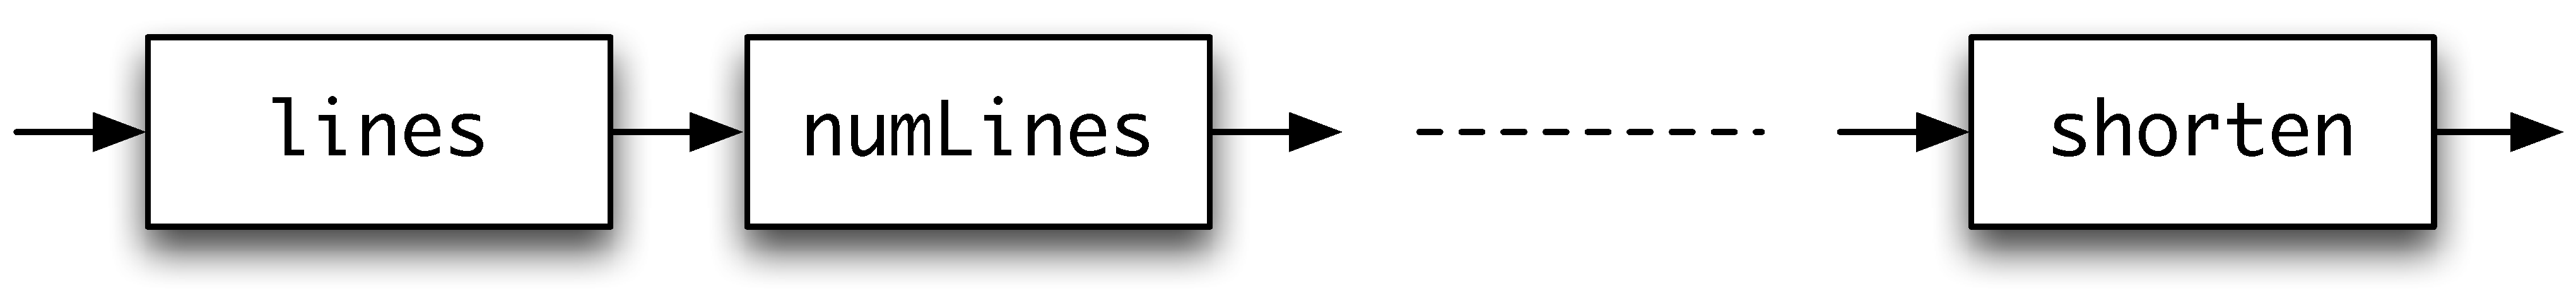
\includegraphics[width=4.5in]{Pictures/pipeline.pdf}
\end{center}
It is easy to see how designs like these can be modified. To take one example,
the indexing program above filters out short words only as its final operation.
There are a number of earlier points in the chain at which this could have been
done, and it is a worthwhile exercise to consider these.

\begin{exercises}


\item
Define the function \texttt{lines} using the functions \texttt{getUntil} and 
\texttt{dropUntil} from Chapter \ref{patternsGen}, or the built-in functions \texttt{takeWhile}
and \texttt{dropWhile}. You should be careful that your functions do not give an
empty word when there are empty lines in the \texttt{Doc}; this might happen for the
examples \texttt{"cat\bs{n}\bs{n}dog"} and \texttt{"fish\bs{n}"}.

\item
How would you use lambda expressions to replace the local definitions in
\texttt{makeLists} and \texttt{shorten}? How would you define these
functions using list comprehensions?

\item
In the index for this book, instead of printing an entry like
\begin{alltt}
cathedral        3, 5, 6, 7, 9, 10
\end{alltt}
a number of ranges could be given:
\begin{alltt}
cathedral        3, 5-7, 9-10
\end{alltt}
How would you redesign your program to do this? Hint: first think about the type
of the new index representation and then consider adding
another function to the (forward) composition which currently forms the
definition of \texttt{makeIndex}.


\item 
How would you re-define \texttt{sortLs} so that duplicate copies of an item are
{\em not\/} removed? For the index, this means that if a word occurs twice on line
\texttt{123} say, then \texttt{123} occurs twice in the index entry for that word.

\item
How could the functions \texttt{getUntil} and \texttt{dropUntil} be used in the
definition of \texttt{amalgamate}?

\item
Explain how the function \texttt{sizer} defined locally in \texttt{shorten}
can be defined as a composition of
built-in functions and operator sections; the role of \texttt{sizer} is
to pick the second half of a pair, find its length, and compare the result
with \texttt{4}.

\item
How is the following definition of the last conditional
equation for \texttt{amalgamate}
incorrect? Give an example calculation to justify your answer.
\begin{alltt}
amalgamate ((l1,w1):(l2,w2):rest)
  | w1 /= w2    = (l1,w1) : amalgamate ((l2,w2):rest)
  | otherwise   = (l1++l2,w1) : amalgamate rest
\end{alltt}

\item
Give a definition of
\begin{alltt}
printIndex :: [ ([Int],Word) ] -> IO ()
\end{alltt}
which gives a neatly laid-out printable version of an index, as shown at
the start of the section. You might find it useful to define a function 
\begin{alltt}
showIndex :: [ ([Int],Word) ] -> String
\end{alltt}
and to use this as a part of your definition of \texttt{printIndex}.

\item 
Modify the program so that words of less than four letters are removed
as a part of the
definition of \texttt{allNumWords}.

\item 
Modify the \texttt{makeIndex} function so that instead of
returning the list of line numbers on which a word occurs, the function
returns
the total number of times that the word occurs. You will need to make
sure that multiple occurrences of a word in a single line are counted. There
are two ways of tackling the problem.
\begin{titemize}
\item Modify the program as little as is necessary -- you could return the
length of a list rather than the list itself, for instance.
\item Take the program structure as a guide, and write a (simpler) program
which calculates the number of occurrences directly.
\end{titemize}

\item
Modify the program so that capitalized words like \texttt{"Dog"} are indexed under
their uncapitalized equivalents (\texttt{"dog"}). This does not work well for
proper names like \texttt{"Amelia"} --- what could you do about that?

\item
The function \texttt{sortLs} is limited to sorting lists of type 
\texttt{[(Int,Word)]} because it calls the \texttt{orderPair} function. Redefine the
function so that it takes the comparison function as a {\em parameter}. What is
its type after this redefinition?
\index{document index|)}

\item 
How would you modify the program if it was to be used to form the index
for a Haskell script? Hint: you need to think about what it is sensible to
ignore in such an enterprise.
\end{exercises}



\section{Development in practice}
\index{program development!in practice|(}

This section goes back to the advice on design and programming
from Chapter \ref{writingProgs} and illustrates how it can be used in a series of
programming examples.

\subsection*{Generalizing the problem}
\index{generalization}

Suppose that we are asked to define the lists \texttt{[1 ..\ n]} for
ourselves. A first attempt might try to use recursion, thus\minx{..}
\begin{alltt}
[1 ..\ n] = 1 : [2 ..\ n]\hfill(..1)
\end{alltt}
but the problem here is that \texttt{[2 ..\ n]} is not an instance of
what we are trying to define. The presence of the \texttt{2} here suggests 
that instead of solving the particular
problem of lists starting at \texttt{1} we should solve the more general problem
of defining lists beginning at an arbitrary value. We therefore define \texttt{[m ..\ n]}:
\begin{alltt}
[m .. n]
  | m>n         = []\hfill(..2)
  | otherwise   = m : [m+1 .. n]
\end{alltt}
Another solution is given by 
\begin{alltt}
[1 .. n] 
  | 1>n         = []\hfill(..3)
  | otherwise   = [1 .. n-1] ++ [n]
\end{alltt}
but \texttt{(..3)} has the disadvantage that it is substantially less
efficient than \texttt{(..2)}, a topic we pick up in Chapter
\ref{behaviour}.

Another example of generalization was given in the text processing
example in Section \ref{textProc} where we defined a function
\texttt{getLine}. The effect of this function is to take a list of words
and to return the list of words making up the maximal first line (of length
\texttt{lineLen}) which can be
built from the words. It was apparent in making the definition that we
needed to make the line length a parameter of the definition, so that
we defined
\begin{alltt}\minx{getLine}
getLine :: Int -> [Word] -> Line
\end{alltt}
rather than giving it the type \texttt{[Word] -> Line}.

\subsection*{Simplifying the problem}
\index{simplification}

Suppose that we are asked to solve the problem of identifying strings
which are palindromes, like
\begin{alltt}\index{palindrome}
"Madam I\bs{'}m Adam"
\end{alltt}
One way of approaching the problem is first to think of identifying
palindromes where punctuation and capitalization are not considered,
such as \texttt{"ABBA"}. We might solve this by
\begin{alltt}
simplePalCheck :: String -> Bool\label{simplePalCheck}
simplePalCheck st = (reverse st == st)
\end{alltt}
for instance, but note that there are at least two other different ways we might
implement the function \texttt{simplePalCheck}. Once we have this function we can
then {\em modify\/} it to solve the original problem. Alternatively we can {\em use\/} 
this solution to a simplified problem in the full solution:
\begin{alltt}\minx{palCheck}
palCheck = simplePalCheck . clean
\end{alltt}
where
\begin{alltt}
clean :: String -> String
\end{alltt}
puts all capitals into small letters and removes punctuation. We look at this in the next section.

\subsection*{Design choices}
\index{design!choices in}

The \texttt{clean} function combines mapping (capitals to smalls) and
filtering (removing punctuation) and so can be solved thus
\begin{alltt}
clean = map toSmall . filter notPunct\hfill(clean.1)
\end{alltt}
or by means of a list comprehension
\begin{alltt}
clean st = [ toSmall ch | ch <- st , notPunct ch ]\hfill(clean.2)
\end{alltt}
How do we choose between these options? One advantage of
\texttt{(clean.1)} is that we see clearly that we have a function
composition, but perhaps \texttt{(clean.2)} is more readable.

\subsection*{Auxiliary functions}

Suppose we are asked to define when one string is a subsequence of
another. By that we mean that the characters of the first string occur
next to each other inside the second string, so that \texttt{"Chip"} is
a subsequence of \texttt{"Fish \& Chips"}, but not of \texttt{"Chin
up"}. The function we seek to define is
\begin{alltt}\minx{subseq}
subseq :: String -> String -> Bool
\end{alltt}
and we try to define this by recursion. Starting with the cases of the
empty string,
\begin{alltt}
subseq []    _  = True
subseq (_:_) [] = False
\end{alltt}
so what is the general case, \texttt{subseq (x:xs) (y:ys)}? 
\begin{itemize}
\item One
alternative is that \texttt{(x:xs)}
is a subsequence of \texttt{ys}, as in \\
\texttt{subseq "Chip" "Fish \& Chips"}
\item The other alternative is that \texttt{(x:xs)} occurs at the start of 
\texttt{(y:ys)}, as in\\
\texttt{subseq "Chip" "Chips"}
\end{itemize}
This latter is not a recursive call to the function we are defining, so
we have to say 
\begin{alltt}
subseq (x:xs) (y:ys)
  = subseq (x:xs) ys || frontseq (x:xs) (y:ys)
\end{alltt}
and write an auxiliary function definition to check this new condition.
\begin{alltt}\minx{frontseq}
frontseq :: String -> String -> Bool
frontseq []     _  = True
frontseq (_:_)  [] = False
frontseq (x:xs) (y:ys)
  = (x==y) \&\& frontseq xs ys
\end{alltt}



\begin{exercises}


\item
Give a recursive definition of the range
\begin{alltt}
[m,n .. p]
\end{alltt}

\item
Think of two more ways of implementing the function
\begin{alltt}
simplePalCheck :: String -> Bool
\end{alltt}
discussed on page \pageref{simplePalCheck}.

\item
Define a function 
\begin{alltt}
subst :: String -> String -> String ->  String
\end{alltt}
so that the result of \texttt{subst start find replace} is the string
\texttt{start}
modified so that the first occurrence of \texttt{find} as a subsequence
is replaced by \texttt{replace}. If there is no such subsequence, the
string should be returned unmodified, so that, for instance,
\begin{alltt}
subst "Fish \& Chips" "Chip" "Boat" \step "Fish \& Boats"
subst "Fish \& Chips" "Ship" "Boat" \step "Fish \& Chips"
\end{alltt}
Modify the definition so that every occurrence of \texttt{find} is
replaced by \texttt{replace}.
Explain what your original and modified definitions do in the case of the example 
\begin{alltt}
subst "Fish \& Chips" "" "Boat"
\end{alltt}
\index{program development!in practice|)}
\end{exercises}

\section{Understanding programs}
\label{understanding}
\index{understanding programs}

This section offers advice to readers confronted with an 
unfamiliar function definition. There are various things we can do 
with the definition, and these are examined in turn here.
Given a functional program like
\begin{alltt}
mapWhile :: (a -> b) -> (a -> Bool) -> [a] -> [b]\minx{mapWhile}
\bl
mapWhile f p []    = [] \hfill (mapWhile.1)
mapWhile f p (x:xs)
  | p x            = f x : mapWhile f p xs \hfill (mapWhile.2)
  | otherwise      = [] \hfill (mapWhile.3)
\end{alltt}
we can understand what it means in various different ways. We can read
the program itself, we can write calculations of examples using
the program, we can prove properties of the program, and we can
estimate its space and time complexity,

\subsection*{Reading the program}
Besides any comments which might accompany a program, the program itself is
its most important documentation. 

The type declaration\index{type declaration}
gives information about
the input and output types: for \texttt{mapWhile}, we have to supply three
arguments:
\begin{titemize}
\item a function, \texttt{f} say, of arbitrary type, \texttt{a -> b};
\item a \textbf{property\/} of objects of type \texttt{a}; that is a function
taking an \texttt{a} to a Boolean value; and,
\item a list of items of type \texttt{a}.
\end{titemize}
The output is a list of elements of type \texttt{b} --
the output type of \texttt{f}.

The function definition itself is used to give values of \texttt{mapWhile}, but
also can be read directly as a description of the program.
\begin{titemize}
\item On \texttt{[]}, the result is \texttt{[]}.
\item On a non-empty list, if the head \texttt{x} has property \texttt{p}, then
according to \texttt{(mapWhile.2)}, we have \texttt{f x} as the first element of the
result, with the remainder given by a recursive call on \texttt{xs}.
\item If the property \texttt{p} fails of \texttt{x}, the result is terminated, as
it were, by returning the empty list \texttt{[]}.
\end{titemize}
In the definition we have a complete description of how the program behaves,
but we can animate this by trying specific examples.


\subsection*{Calculating with the program}
\index{calculation}

A more concrete view of what the program does is given by calculating
particular examples. For instance,
\begin{alltt}
mapWhile (2+) (>7) [8,12,7,13,16]
\step 2+8 : mapWhile (2+) (>7) [12,7,13,16] \hfill {\rm by} (mapWhile.2)
\step 10 : 2+12 : mapWhile (2+) (>7) [7,13,16] \hfill {\rm by} (mapWhile.2)
\step 10 : 14 : [] \hfill {\rm by} (mapWhile.3)
\step [10,14]
\end{alltt}
Other examples include
\begin{alltt}
mapWhile (2+) (>2) [8,12,7,13,16] \step [10,14,9,15,18]
mapWhile (2+) (>2) []             \step []
\end{alltt}
Note that in these examples we use \texttt{mapWhile} at the instance
\begin{alltt}
(Int -> Int) -> (Int -> Bool) -> [Int] -> [Int]
\end{alltt} 
of its polymorphic type,
given by replacing the type variables \texttt{a} and \texttt{b} by the type 
\texttt{Int}.

\subsection*{Reasoning about the program}
\index{proof}

We can get a deeper understanding about a program by \textbf{proving} properties
that the program might have. For \texttt{mapWhile}, we might prove that for all
\texttt{f}, \texttt{p} and finite lists \texttt{xs},
\begin{alltt}
mapWhile f p xs            = map f (takeWhile p xs)\hfill(mapWhile.4)
mapWhile f (const True) xs = map f xs\hfill(mapWhile.5)
mapWhile id p xs           = takeWhile p xs\hfill(mapWhile.6)
\end{alltt}
where we can, in fact, see \texttt{(mapWhile.5)} and \texttt{(mapWhile.6)} as consequences of the
characterization of \texttt{mapWhile} given by property \texttt{(mapWhile.4)}. 

Rather than proving these properties, it is possible to use QuickCheck to test them with random data. Recall the discussion in the breakout box `QuickCheck and higher-order functions'  on page \pageref{QChofs},\index{QuickCheck} which outlines how functions of this sort can be tested on a selection of functional arguments and randomly-generated list data.


\subsection*{Program behaviour}
\index{behaviour}
It is not hard to see that the program will at worst take time linear (that is
\texttt{O(n\uppp{1})}) in the length (\texttt{n}) of the list argument assuming \texttt{O(n\uppp{0})}
behaviour of \texttt{f} and \texttt{p}, as it runs through the elements of the list
once, if at all.

The \textbf{space\/} behaviour is more interesting; because we can output the
head of a list once produced, the space required will be constant, as
suggested by underlining the parts which can be output in the calculation
above.
\begin{alltt}
mapWhile (2+) (>7) [8,12,7,13,16]
\step 2+8 : mapWhile (2+) (>7) [12,7,13,16] 
\step \underline{10} : 2+12 : mapWhile (2+) (>7) [7,13,16] 
\step \underline{10 : 14} : [] 
\step \underline{[10,14]}
\end{alltt}
We return to a fuller discussion of program behaviour in Chapter \ref{behaviour}.

\subsection*{Getting started}

Each view of the program gives us a different understanding of its
behaviour, but when we are presented with an unfamiliar definition we can
begin to understand what its effect is by calculating various small examples.
If we are given a collection of functions, we can test out the functions from
the bottom up, building one calculation on top of another, using GHCi as a calculator. 
 
The important
thing is to realize that rather than being stuck, we can get started by
calculating representative examples to show us the way.

\begin{summary}
This chapter has explored the idea that program development works in a cycle: first we
clarify the specification of the problem to be solved, next we devise a
plan of how to solve the problem, and only then do we implement the
solution. 

At each stage we should reflect on and evaluate what we have
done: this aspect is crucial particularly when we are learning to
program. For example, being aware of the errors that we make can help us to prevent
making them in the future. Also, if we take a problem we have already solved and 
try to solve it with a new technique we will learn something about the new technique
as well as seeing how it fits in with what we have learned already. This is
something that we do by continually revisiting the \texttt{Picture}
case study.

\index{program development|)}
\end{summary}

%\end{document}

%\documentclass{book}\usepackage{sjtfonts}\usepackage{includegraphics}\usepackage{alltt}\usepackage{latexsym}
%\usepackage{array}
%\begin{document}\input{defs0}%		miradefs.tex 		    June 1994

% opening and closing a quoted Miranda section

\newcommand{\mira}{\noindent\hrulefill\nopagebreak\so}
\newcommand{\arim}{\nopagebreak\st\hrulefill\\}

% backslash in the Miranda environment
% Only feasible approach is to use \verb+\+
% in line!

%\newcommand{\bs}{$\mi\backslash\!\!$}
%\newcommand{\lbs}{\mbox{\verb+\+}}

% ignoring part of the input

\newcommand{\ignore}[1]{}

% a blank line in a Miranda section

\newcommand{\bl}{\mbox{\ }}

% Signalling a diffculty.

\definecolor{light-gray}{gray}{0.95}

\newcommand{\beware}[2]
 {\medskip\noindent\colorbox{light-gray}{\parbox{\textwidth}
 {\mbox{\large\textbf{#1}} \medskip\noindent\\ #2}\medskip\noindent}}

% Subscripting in Miranda text
\newcommand{\subscr}[2]{\mbox{${\mbox{\texttt{#1}}}_{\mbox{\texttt{#2}}}$}}

%\newcommand{\subscr}[2]{\mbox{${\mbox{\mi #1}}_{\mbox{\smtt #2}}$}}
\newcommand{\aone}{\subscr{a}{1}}
\newcommand{\atwo}{\subscr{a}{2}}
\newcommand{\ak}{\subscr{a}{k}}

\newcommand{\aoneone}{\subscr{a}{1,1}}

\newcommand{\eone}{\subscr{e}{1}}
\newcommand{\etwo}{\subscr{e}{2}}
\newcommand{\ei}{\subscr{e}{i}}
\newcommand{\er}{\subscr{e}{r}}

\newcommand{\fone}{\subscr{f}{1}}
\newcommand{\fl}{\subscr{f}{l}}

\newcommand{\gone}{\subscr{g}{1}}
\newcommand{\gtwo}{\subscr{g}{2}}
\newcommand{\gi}{\subscr{g}{i}}
\newcommand{\gr}{\subscr{g}{r}}

\newcommand{\hone}{\subscr{h}{1}}
\newcommand{\hl}{\subscr{h}{l}}

\newcommand{\pone}{\subscr{p}{1}}
\newcommand{\ptwo}{\subscr{p}{2}}
\newcommand{\pk}{\subscr{p}{k}}

\newcommand{\qone}{\subscr{q}{1}}
\newcommand{\qtwo}{\subscr{q}{2}}
\newcommand{\qk}{\subscr{q}{k}}

\newcommand{\rone}{\subscr{r}{1}}
\newcommand{\rtwo}{\subscr{r}{2}}

\newcommand{\tone}{\subscr{t}{1}}
\newcommand{\ttwo}{\subscr{t}{2}}
\newcommand{\tn}{\subscr{t}{n}}

\newcommand{\vone}{\subscr{v}{1}}
\newcommand{\vtwo}{\subscr{v}{2}}
\newcommand{\vn}{\subscr{v}{n}}

% for regular expressions

\newcommand{\stone}{\subscr{st}{1}}
\newcommand{\sttwo}{\subscr{st}{2}}
\newcommand{\stn}{\subscr{st}{n}}
\newcommand{\rthree}{\subscr{r}{3}}

\newcommand{\eps}{$\varepsilon$}
\newcommand{\trans}[1]{\stackrel{\mbox{\tt #1}}{\longrightarrow}}



% superscript in Miranda text

\newcommand{\superscr}[2]{\mbox{${\mbox{\mi #1}}^{\mbox{\smtt #2}}$}}

% Not equals in Miranda text

\newcommand{\noteq}{\makebox[0pt][l]{=}/}
\newcommand{\overslash}{\makebox[0pt][l]{/}}

% Definitions in complexity chapter

\newfont{\oldSym}{cmsy10}
\newcommand{\Th}{\boldmath$\oldSym\Theta$}
\newcommand{\pow}[1]{\^{}#1}
\newcommand{\leqq}{$\leq$}
\newcommand{\geqq}{$\geq$}
\newcommand{\lll}{$\ll$}
\newcommand{\eqq}{$\equiv$}
\newcommand{\ltwo}{\subscr{log}{2}}

% Indexing

\newcommand{\minx}[1]{\index{#1@{\ttfamily{}#1}}}
\setcounter{chapter}{11}\setcounter{page}{201}

\chapter{Overloading, type classes and type checking}
\chapstart
\label{typeClasses}\label{types}
\label{classes}
\index{classes|(}
\index{type classes|see{classes}}

In looking at Haskell so far we have seen two kinds of function which
work over more than one type.
A polymorphic function such as \texttt{length} has a \emph{single}
definition which works over all its types. On the other hand, 
\textbf{overloaded}\index{function!overloaded|see{overloading}}\index{overloading}
functions like equality, \texttt{+} and \texttt{show} can be used at a
variety of types, but with different definitions at the different
types. 

The chapter starts with a discussion of the benefits of overloading, before looking at 
\textbf{type classes}, which are collections of types; what the
members of a class have in common is the fact that certain functions are
defined over the type. For instance, the members of the equality type
class, \texttt{Eq}, are those types which carry an equality function,
\texttt{==}. Type classes are thus the mechanism by which overloaded
functions can be given types in Haskell.

We shall see how to define type classes and types which belong to these
classes: the \textbf{instances} of the class. 
Haskell's prelude and libraries contain a number of classes and
instances, particularly for numeric types -- we survey these, referring
readers to the Haskell report \cite{haskell2010} for a full exposition.


We then look at how type inference and type checking work in Haskell, first looking at types without type variables -- monomorphic definitions -- and then at polymorphic, overloaded definitions, and see how they are given types, illustrated by a series of examples.

\section{Why overloading?}
\index{overloading!reason for}
\label{whyOver}

This section looks at the reason for including overloading in Haskell;
we do this by looking at a scenario.

Suppose that Haskell did not have overloading, and that we wanted to
check whether a particular element is a member of a list of type
\texttt{Bool}. We would define a function like
\begin{alltt}\minx{elemBool}
elemBool :: Bool -> [Bool] -> Bool
elemBool x [] = False
elemBool x (y:ys)
  = (x \subscr{==}{Bool} y) || elemBool x ys
\end{alltt}
where we have written \texttt{\subscr{==}{Bool}} for the equality 
function over \texttt{Bool}. 

Suppose now that we want to check whether
an integer is a member of an integer list, then we need to define a
\textit{new}
function 
\begin{alltt}\minx{elemInt}
elemInt :: Int -> [Int] -> Bool
\end{alltt}
which differs from \texttt{elemBool} only in using \texttt{\subscr{==}{Int}}
instead of \texttt{\subscr{==}{Bool}}. Each time we want to check
membership of a list of a different type we will have to define yet
another -- very similar -- function. 
One way out of this problem is to make the equality function a parameter
of a general function 
\begin{alltt}
elemGen :: (a -> a -> Bool) -> a -> [a] -> Bool
\end{alltt} but this gives too much
generality, because it can be used with {\em any\/} parameter of type
\texttt{a -> a -> Bool} rather than just an equality function. More importantly, using this definition the parameter has to be passed in explicitly each time the
function \texttt{elemGen} is used, like this
\begin{alltt}
elemGen (\subscr{==}{Bool})
\end{alltt}
making programs less easy to read.\footnote{In fact, the implementation of classes works like this, passing in a \emph{dictionary} argument containing the appropriate equality function at each point that \texttt{elem} is used, after it has been transformed into  \texttt{elemGen}.}
The alternative is to define a function which uses the overloaded
equality,
\begin{alltt}
elem :: a -> [a] -> Bool
\end{alltt}
where the type \texttt{a} \emph{has to be restricted to those types \texttt{a} which have
an equality}. The advantages of this approach are
\begin{itemize}
\item{\bf Reuse}\hskip 1em The definition of \texttt{elem} can be used over all types
with equality.
\item{\bf Readability}\hskip 1em It is much easier to read \texttt{==} than
\texttt{\subscr{==}{Int}} and so on. This argument holds particularly for numeric operators, where
it is more than tiresome to have to write \texttt{\subscr{+}{Int}},
\texttt{\subscr{*}{Float}} and so on.
\end{itemize}
What this discussion shows is that a mechanism is needed to give a type
to functions like \texttt{elem}: that is precisely the purpose of type
classes.

\section{Introducing classes}
\index{classes}

The \texttt{elem} function appears to have the type
\begin{alltt}
elem :: a -> [a] -> Bool
\end{alltt}
\emph{but} \texttt{elem} \emph{only has this type for types} \texttt{a} \emph{which have an equality
function}. How is this to be expressed?
We need some way of saying whether we have an equality
function over a given type. We call the collection of types over which a
function is defined a \textbf{type class} or simply a \textbf{class}. For instance, 
the set of types over which \texttt{==} is
defined is the \textbf{equality class}, \texttt{Eq}.
\minx{Eq}

\subsection*{Defining the equality class, \texttt{Eq}} 
\index{equality}

How do we define a class, such as \texttt{Eq}? 
We say what is needed for a type 
\texttt{a} to be in a class. In this case we need a function \texttt{==} defined
over \texttt{a}, of type \texttt{a->a->Bool}. 
\begin{alltt}\minx{class}
class Eq a where
  (==) :: a -> a -> Bool
\end{alltt}
In general we will specify an \textbf{interface} or  \textbf{signature} which has to be implemented for a type to belong to the class.

Members of a type class are called its
\textbf{instances}, and a type is made into an instance by giving an implementation of the interface for that type. This is called an instance declaration.
Built-in instances of \texttt{Eq}\index{instance!of class}\index{classes!instance}
include the base types
\texttt{Int}, \texttt{Float}, \texttt{Bool}, \texttt{Char}. Other instances are given by
tuples and lists
built from types which are themselves instances of \texttt{Eq}; examples include
the types \texttt{(Int,Bool)} and \texttt{[[Char]]}. 

Not all types will necessarily
carry an equality; we may choose not to define one, for reasons of information
hiding, or there may be no natural way of defining an equality on a particular
type. 

For example, function
types like \texttt{Integer -> Integer} are not instances of
\texttt{Eq}, since there is no way that we can write a program which will decide
whether two functions over \texttt{Integer} have the same behaviour, that is have the same values at every possible input.


\beware{`Instances' in Haskell}{
It is unfortunate that the term {\em instance\/} is used in two
\index{instance!different meanings in Haskell}
different ways in Haskell. We talked in Section \ref{poly}
of a type \texttt{\subscr{t}{1}}
being an instance of a
{\em type\/} \texttt{\subscr{t}{2}}, when we can substitute for a type
variable in \texttt{\subscr{t}{2}} to give \texttt{\subscr{t}{1}}. Here we have
talked about a type being an instance of a {\em class}. It should be clear which one we mean from the context of a discussion, but it's helpful to bear this `overloading' of terminology in mind.}

\subsection*{Functions that use equality}

Many of the functions which we have defined so far use equality
over particular types. The function 
\begin{alltt}\minx{allEqual}
allEqual :: Int -> Int -> Int -> Bool
allEqual m n p = (m==n) \&\& (n==p)
\end{alltt}
decides whether three integers are equal. If we examine the definition
itself, it contains nothing which is specific to integers; the only constraint
it makes is that \texttt{m}, \texttt{n} and \texttt{p} are compared for equality. Their
type can be \texttt{a} \emph{for any \texttt{a} in the type class} \texttt{Eq}. This
gives \texttt{allEqual} a most general type thus:
\begin{alltt}\index{\symbol{61}\symbol{62}@\texttt{\symbol{61}\symbol{62}}}
allEqual :: Eq a => a -> a -> a -> Bool
allEqual m n p = (m==n) \&\& (n==p)
\end{alltt}
The part before the \texttt{=>} is called the \textbf{context}. We can read the type
\index{context}
as saying that 
\begin{quote}
\texttt{allEqual} has type
\texttt{a -> a -> a -> Bool} for all types \texttt{a} in the class \texttt{Eq} (that is,  all types \texttt{a} for which \texttt{==} is defined)
\end{quote}
This means that \texttt{allEqual} can be used at many types, including these
\begin{alltt}
allEqual :: Char -> Char -> Char -> Bool
allEqual :: (Int,Bool) -> (Int,Bool) -> (Int,Bool) -> Bool
\end{alltt}
since both \texttt{Char} and \texttt{(Int,Bool)} belong to \texttt{Eq}.

What happens if we break this constraint by trying
to compare three functions for equality? If we define
\index{errors!and classes}
\begin{alltt}
suc :: Integer -> Integer
suc = (+1)
\end{alltt}
and try to evaluate
\begin{alltt}
allEqual suc suc suc 
\end{alltt}
in GHCi we get the message\index{type error!instance error}
\begin{alltt}
    No instance for (Eq (Integer -> Integer))
      arising from a use of `allEqual' at <interactive>:1:0-19
    Possible fix:
      add an instance declaration for (Eq (Integer -> Integer))
    In the expression: allEqual suc suc suc
    In the definition of `it': it = allEqual suc suc suc
\end{alltt}
which conveys the fact that \texttt{(Integer -> Integer)} is not in the \texttt{Eq} class, and suggests that the way to fix the problem is to add an instance declaration for that type. 

\subsection*{More equality examples}

The \texttt{elem} example in Section \ref{whyOver} will have the type
\begin{alltt}
elem :: Eq a => a -> [a] -> Bool
\end{alltt}
and so it will be usable at the types
\begin{alltt}
Bool -> [Bool] -> Bool
Int  -> [Int]  -> Bool
\end{alltt}
and so on. Many of the functions we have defined already use equality in an
overloaded way. We can
use GHCi to deduce the most general type of a function, such as
the
\texttt{books} function from the library database of Section \ref{library},
by commenting out its type declaration in the script, thus
\begin{alltt}
-- books :: Database -> Person -> [Book]\minx{books}
\end{alltt}
and then by typing\index{type@\texttt{:type}}
\begin{alltt}
:type books
\end{alltt}
to the prompt. The result we get in that case is
\begin{alltt}
books :: Eq a => [ (a,b) ] -> a -> [b]\minx{books}
\end{alltt}
which is perhaps a surprise at first. This is less so if we rewrite the
definition with \texttt{books} renamed \texttt{lookupFirst},
because it looks up all the pairs with a particular first part, and returns
their corresponding second parts. Here it is with its variables renamed
as well
\begin{alltt}\minx{lookupFirst}
lookupFirst :: Eq a => [ (a,b) ] -> a -> [b]
\bl
lookupFirst ws x 
  = [ z | (y,z) <- ws , y==x ]
\end{alltt}
Clearly from this definition there is nothing specific about books or
people
and so it is polymorphic, if we can compare objects in the first halves of the
pairs for equality. This condition gives rise to the context \texttt{Eq a}.
Finally from Section \ref{library}, as we saw for \texttt{books},
\begin{alltt}
borrowed    :: Eq b => [ (a,b) ] -> b -> Bool\minx{borrowed}
numBorrowed :: Eq a => [ (a,b) ] -> a -> Int\minx{numBorrowed}
\end{alltt}

\begin{summary}
In this section we have introduced the idea of a class, which is a collection
of types, its instances, with the property that certain functions described in an interface are
defined over the type. One way we can think of a class is as an \textbf{adjective}: 
any particular type is or is not in the class, just as the 
\index{classes!as adjective}
weather at any particular moment might or might not be sunny.

We saw how equality could be seen as being defined over all the types in the
class \texttt{Eq}. This allows many of the functions defined so
far to be given polymorphic type, allowing them to be used over any type in
the class \texttt{Eq}. In the following sections we explain how classes and
instances are defined in general, and explore the consequences of classes for
programming in Haskell.
\end{summary}

\begin{exercises}

\item
How would you define the `not equal'
operation, \texttt{/=}, from equality, \texttt{==}? What is the type of
\texttt{/=}?

\item
Define the function \texttt{numEqual} which takes a list of items, \texttt{xs} say,
and an item, \texttt{x} say, and returns the number of times \texttt{x} occurs in
\texttt{xs}. What is the type of your function? How could you use \texttt{numEqual}
to define \texttt{member}?

\item
Define functions
\begin{alltt}
oneLookupFirst  :: Eq a => [ (a,b) ] -> a -> b
oneLookupSecond :: Eq b => [ (a,b) ] -> b -> a
\end{alltt}
\texttt{oneLookupFirst} takes a list of pairs and an item, and returns the second
part of the first pair whose first part equals the item. You
should explain what your function does if there is no such pair. 
\texttt{oneLookupSecond} returns the first pair with the roles of first and second
reversed.
\end{exercises}

\section{Signatures and instances}
\label{sigInsts}

In the last section we saw that the operation of equality, \texttt{==}, 
is overloaded. This allows \texttt{==} to be used over a variety of types, and
also
allows for functions using \texttt{==}
to be defined over all instances of the class of types \texttt{Eq}.
This section explains the mechanics of how classes are introduced, and then
how instances of them may be declared. This allows us to
program with classes that we define ourselves, rather than simply using the
built-in classes of Haskell.


\subsection*{Declaring a class}

As we saw earlier, a class is introduced by a declaration like:
\begin{alltt}
class Info a where\minx{class}\minx{Info}
  examples :: [a]
  size     :: a -> Int
\end{alltt}
The declaration introduces the name of the class, \texttt{Info}, and this is
followed by an \textbf{interface} or signature, that is a list of identifiers and their types. To be in the \texttt{Info} class the type
\index{signature}\index{interface}
\texttt{a} must carry the two bindings in the
\minx{Info}
signature:
\begin{titemize}
\item the \texttt{examples} list, which is a list of objects of type \texttt{a}, which we can think of as giving a list of representative examples from the type, and,
\item the \texttt{size} function, which returns a measure of the size of the
argument, as an integer.
\end{titemize}
The general form of a class definition will be:
\begin{alltt}\index{classes!general form of definition}
class Name ty where
  ... signature involving the type variable ty ...
\end{alltt}
Now, how are types made instances of such a class?

\subsection*{Defining the instances of a class}

A type is made a member or \textbf{instance} of a class by defining
the interface functions for the type. For example,
\begin{alltt}
instance Eq Bool where\minx{instance}\index{classes!instance}\minx{Eq}
  True  == True  = True
  False == False = True
  _     == _     = False
\end{alltt}
describes how \texttt{Bool} is an instance of the equality class. The
declarations that numeric types like \texttt{Int} and \texttt{Float} are in the
equality class (and indeed other built-in classes) involve the appropriate
primitive
equality functions supplied by the implementation. 

Although we have called the class \texttt{Eq} the equality class, there is
no requirement that the \texttt{==} function we define has any of the usual
properties of equality apart from having the same type as equality. It is up
to the user to ensure that he or she makes sensible definitions, and documents
them adequately.

Going back to our \texttt{Info} example, we might say
\begin{alltt}
instance Info Char where\minx{Info}
  examples = ['a','A','z','Z','0','9']
  size _   = 1
\end{alltt}
This gives a list of six typical characters and states that each character is of size one. We can also make \texttt{Bool} and \texttt{Int} instances of \texttt{Info}, like this:
\begin{alltt}
instance Info Bool where
  examples = [True,False]
  size _   = 1
  
instance Info Int where
  examples = [-100..100]
  size _   = 1  
\end{alltt}
In the \texttt{examples} for \texttt{Bool} we can list all the elements, for integers we choose a range of ``small'' numbers; as for characters, we say each object is of size one. Finally we can look at the \texttt{data} type of \texttt{Shape}s, and declare an instance for them:
\begin{alltt}
instance Info Shape where
  examples = [ Circle 3.0, Rectangle 45.9 87.6 ]
  size     = round . area
\end{alltt}
Here we just list a couple of typical shapes, and use the \texttt{area}, rounded to an integer, as an indication of size

\subsubsection*{Instances and contexts}

Suppose that the type \texttt{a} is in the \texttt{Info} classs: this means that
we can estimate the size of a value in
\texttt{a}, and we have a list of examples of type \texttt{a}. Using this function and list we are able to define a \texttt{size} function for \texttt{[a]} and a list of examples of type \texttt{[a]} like thisto define those
functions over \texttt{[a]}, so we can declare the following instance
\begin{alltt}\index{context}
instance Info a => Info [a] where ....
\end{alltt}
in which the\index{classes!context}
\textbf{context} \texttt{Info a} appears, making clear that we are only providing information about lists of objects for which we already have information about the individual members.

\begin{figure}[t]\index{errors!type error messages}
\beware{Type error messages}{
We first saw the example of a type error message mentioning `instances' in Section \ref{errors} where the application \texttt{4 double} gave rise to the error message
\begin{alltt}
\ \ \ \ No instance for (Num ((Integer -> Integer) -> t))

\ \ \ \ \ \ arising from the literal `4' at <interactive>:1:0-7
    ...
\end{alltt}
instead of the simple message ``attempt to apply a number to a function''.

\medskip
The problem is that we \emph{could} have overloaded the numbers to have this sort of behaviour, but common sense suggest that we haven't; it's difficult, though, to get error messages to reflect common sense, because it it inconsistent and context-dependent. At least, though, we can now understand what is being said in the error message, even if the appropriate course of action is quite different \ldots\ .
}
\end{figure}

We can complete the
definition like this
\begin{alltt}\label{visiDec}
instance Info a => Info [a] where
  examples = [ [] ] ++ 
             [ [x] | x<-examples ] ++ 
             [ [x,y] | x<-examples , y<-examples ]
  size     = foldr (+) 1 . map size  
\end{alltt}
Out list of examples is made up by the empty list, together with all the one and two element lists that can be built up from the \texttt{examples} of type \texttt{a}. So, in this definition we see overloading in action: on the left hand side of the \texttt{examples} is used at type \texttt{[a]}, while on the right hand side the three occurrences are all at type \texttt{a}.

To estimate the size of a list of \texttt{a} we
take the size of each element (\texttt{map size}), and add one to the total of
these sizes using \texttt{foldr (+) 1}. Again, on the 
right-hand side of this
definition we use \texttt{size} over the type \texttt{a}; this
shows that we need the context which says that \texttt{a} is in the \texttt{Info}
class.

\subsubsection*{Limitations}\index{classes!limitations}

Instances in Haskell are \emph{global}, so that once you have declared an instance for a type, that instance is the one that you will have to use with that type: in particular it isn't possible to make instances \emph{local} to a module or set of modules. If you still want to do this, the mechanism to use would be to define a `wrapped' type, like
\begin{alltt}
data WInt = Wrap Int
\end{alltt}
and to declare the instances you want for this type of integers.

There are also some limitations to what can be declared as an instance, in other
words on what can appear after the \texttt{=>} (if any) in an instance
declaration. This must either be a base type like \texttt{Int}, or consist of a
type constructor like \texttt{[...]}, \texttt{(...,...)} or \texttt{Shape} applied to
distinct type variables.

We will {\em not\/} be able, for example, to declare
\texttt{(Float,Float)} as an instance; nor can we use named types (introduced by
a \texttt{type} definition). More details of the mechanism can be found in the
Haskell 2010 report \cite{haskell2010}.

\beware{Haskell 2010 \emph{vs.}\ GHC Haskell}{\index{Haskell 2010!and GHC Haskell}
In fact, GHC implements a more flexible mechanism for type classes and instances, and choosing this option within GHC or GHCi using the flag \texttt{-XFlexibleInstances} allows us to move away from Haskell 2010. This can be achieved by putting this as the first line in a Haskell file, preceding the \texttt{module} declaration:
\begin{alltt}
\{-\# OPTIONS\_GHC -XFlexibleInstances \#-\}
\end{alltt}

The problem with doing this is that your program becomes reliant on GHC rather than Haskell 2010, which is supported by a number of compilers, and also runs the risk of depending on a feature which might change. Sufficiently many Haskell programmers are prepared to take little risks like this that it is difficult to find a project of any size which is fully Haskell 2010 compliant.
}



\subsection*{Default definitions}

\index{classes!default definitions}
To return to our example of equality, the Haskell equality class is in fact
defined by
\begin{alltt}
class Eq a where
  (==), (/=) :: a -> a -> Bool
  x /= y     = not (x==y)
  x == y     = not (x/=y)
\end{alltt}
To the equality operation is added inequality, \texttt{/=}. As well as this,
there are \textbf{default} definitions of \texttt{/=} from \texttt{==} and of \texttt{==} from
\texttt{/=}. These definitions have
two purposes; they give a definition over all equality types, but as
defaults
they can \textbf{overridden} by an \texttt{instance} declaration. 

At any
instance a definition of at least one of \texttt{==} and
\texttt{/=} needs to be supplied for there to be a proper definition of (in)equality, but a
definition of either is sufficient to give both, by means of the
defaults.

It is also possible to define both of the operations in an instance
delaration , so that if we wanted to
define a different version of \texttt{/=} over \texttt{Bool}, we could add to our
instance declaration for \texttt{Bool} the line
\begin{alltt}
  x /= y     = ... our definition ...
\end{alltt}
In our \texttt{Info} example you will probably have noticed that for many of the base types we simply said that the \texttt{size} of all the objects was one; we can add this as a default to the definition of \texttt{Info} like this:
\begin{alltt}\minx{Info}
class Info a where
  examples :: [a]
  size     :: a -> Int
  size _   = 1
\end{alltt}
and then the declarations for \texttt{Int}, \texttt{Char} and \texttt{Bool} become  
\begin{alltt}
instance Info Int where
  examples = [-100..100]

instance Info Char where
  examples = ['a','A','z','Z','0','9']

instance Info Bool where
  examples = [True,False]
\end{alltt}

\beware{Default or top-level?}{\index{instance!default}
If we want to \emph{stop} a default being overridden, we should remove
the operation from the class, and instead give its
definition at the
top level and not in the signature. In the case of the operation \texttt{/=} in
\texttt{Eq} we would give the top-level definition
\begin{alltt}
x /= y       = not (x == y)
\end{alltt}
which has the type 
\begin{alltt}
(/=) :: Eq a => a -> a -> Bool
\end{alltt}
and will be effective over all types which carry the \texttt{==} operation.

\medskip
There are some situations when it is better to give
default definitions, which can be overridden, rather than top-level
definitions, which cannot. Over the numerical types, for instance, an
implementation may well supply all the operations as hardware instructions,
which will be much more efficient than the default definitions.
}


\subsection*{Derived classes}

\index{classes!derived}
Functions and instances can depend upon types being in classes; this is also
true of classes. The simplest example in Haskell is the class of ordered
types,
\texttt{Ord}. To be ordered, a type must carry the operations \texttt{>}, \texttt{>=}
and so on, as well as the equality operations. We say
\begin{alltt}
class Eq a => Ord a where\minx{Ord}
  (<), (<=), (>), (>=) :: a -> a -> Bool
  max, min             :: a -> a -> a
  compare              :: a -> a -> Ordering
\end{alltt}
For a type \texttt{a} to be
in the class \texttt{Ord}, we must supply over
\texttt{a} definitions of the operations of
\texttt{Eq} 
as well as the ones in the signature of \texttt{Ord}. Given a definition of 
\texttt{<} we can supply default definitions of the remaining operations of 
\texttt{Ord}.
For instance,
\begin{alltt}
x <= y     = (x < y || x == y)
x >  y     =  y < x
\end{alltt}
We will explain the type \texttt{Ordering} and the function \texttt{compare}
in Section \ref{haskellClasses}.

A simple example of a function defined over types in the class \texttt{Ord} is the
insertion sort function \texttt{iSort} of Chapter \ref{defFunLists}. Its most general type is
\begin{alltt}
iSort :: Ord a => [a] -> [a]\minx{iSort}
\end{alltt}
Indeed, any sorting function (which sorts using the ordering given by 
\texttt{<=}) would be expected to have this type.

From a different point of view, we can see the class \texttt{Ord} as 
\textbf{inheriting} the operations of \texttt{Eq}; inheritance is one of the central\index{inheritance}
\index{object-oriented}
ideas of object-oriented programming.

\subsection*{Multiple constraints}

\index{context!multiple}
In the contexts we have seen so far, we have a single constraint on a type,
such as \texttt{Eq a}. There is no reason why we should not have multiple
constraints on types. This section introduces the notation we use, and some
examples where it is needed.

Suppose we wish to sort a list and then show the results as a string. We can
write
\begin{alltt}
vSort = show . iSort 
\end{alltt}
To sort the elements, we need the list to consist of elements from an ordered
type, as we saw above.
To convert the results to a \texttt{String} we need \texttt{[a]} to be in the \texttt{Show} class (which we discuss in detail in the next section). To do this it is sufficient for each  element of type 
\texttt{a} to be printable, and so the type of \texttt{vSort} is 
\begin{alltt}
vSort :: (Ord a,Show a) => [a] -> String
\end{alltt}
showing that \texttt{a} must be in both the classes \texttt{Ord} and \texttt{Show}.
Such types include \texttt{Bool}, \texttt{[Char]} and so on.

In a similar way, suppose we are to use \texttt{lookupFirst}, and then make the
results visible. We write
\begin{alltt}
vLookupFirst xs x = show (lookupFirst xs x)
\end{alltt}
We have twin constraints again on our list type \texttt{[(a,b)]}. We need to be
able to compare the first halves of the pairs, so \texttt{Eq a} is required. We
also want to turn the second halves into strings, so needing \texttt{Show b}.
This gives the type
\begin{alltt}
vLookupFirst :: (Eq a,Show b) => [(a,b)] -> a -> String
\end{alltt}
Multiple constraints can occur in an instance declaration, such as
\begin{alltt}\index{equality!on pairs}
instance (Eq a,Eq b) => Eq (a,b) where
  (x,y) == (z,w)  =  x==z \&\& y==w
\end{alltt}
which shows that a pair of types in \texttt{Eq} again belongs to
\texttt{Eq}. Multiple constraints can 
also occur in the definition of a class,
\begin{alltt}
class (Ord a,Show a) => OrdShow a
\end{alltt}
In such a declaration, the class inherits the operations of both \texttt{Ord}
and \texttt{Show}.

In this particular
case, the class declaration contains an empty signature. To be
in \texttt{OrdShow}, the type \texttt{a} must simply be in the classes \texttt{Ord} and
\texttt{Show}. We could then modify the type of \texttt{vSort} to say
\begin{alltt}
vSort :: OrdShow a => [a] -> String
\end{alltt}
The situation when a class is built on top of two or more classes is called
\textbf{multiple inheritance}; this has consequences for programming
\index{inheritance!multiple}
style, explored in Section \ref{oop}.


\subsection*{\texttt{infoCheck}: a QuickCheck clone}
\label{infoCheck}\index{infoCheck@\texttt{infoCheck}|(}
\index{QuickCheck!\texttt{infoCheck} clone}

We can define a stripped-down version of QuickCheck for ourselves, using the \texttt{examples} that the \texttt{Info} type class provides. Suppose we have these examples for type \texttt{a}: how do we check that a \texttt{property} of type \texttt{a -> Bool}? We want to check that the \texttt{property} holds for all the examples, so we apply it to all of them, using \texttt{map} and then take their conjunction, using \texttt{and}:
\begin{alltt}
infoCheck :: (Info a) => (a -> Bool) -> Bool

infoCheck property = and (map property examples)\hfill(infoCheck.1)  
\end{alltt}
We could do a similar thing for a two argument property, defining
\begin{alltt}
infoCheck2 :: (Info a, Info b) => (b -> a -> Bool) -> Bool

infoCheck2 property = 
    and (map (infoCheck.property) examples) \hfill(infoCheck.2)  
\end{alltt}
Note that \texttt{infoCheck2} uses \texttt{infoCheck} in its definition. Similarly we can define \texttt{infoCheck3} and so on. We could stop here, but we can do better, using overloading to define a single \texttt{infoCheck} function, just as there is a single \texttt{quickCheck} function.

To do this we define another type class, and say that a type is \texttt{Checkable} if it's something that can be checked by applying it to the \texttt{examples} given in an \texttt{Info} type:
\begin{alltt}
class Checkable b where
 infoCheck :: (Info a) => (a -> b) -> Bool
\end{alltt}
What instances can we define? Well, the definition of \texttt{(infoCheck.1)} is the same as an instance declaration for \texttt{Bool}:
\begin{alltt}
instance Checkable Bool where
  infoCheck property = and (map property examples)  
\end{alltt}
The definition \texttt{(infoCheck.2)} gives us a way of making checkable functions with an additional argument,
\begin{alltt}
instance (Info a, Checkable b) => Checkable (a -> b) where
  infoCheck property = and (map (infoCheck.property) examples) 
\end{alltt}
Taking these together, we have \texttt{infoCheck} defined over all these types:
\begin{alltt}
Bool -> Bool
Shape -> Bool
Int -> Shape -> Bool
Bool -> Int -> Shape -> Bool
\end{alltt}
In short, we can apply \texttt{infoCheck} to any type where the argument types are in the \texttt{Info} class, and where the result is a \texttt{Bool}, just as in the original definition of the \texttt{quickCheck} function.

\index{infoCheck@\texttt{infoCheck}|)}



\begin{summary}
This section has explained the basic details of the class mechanism in
Haskell. We have seen that a class definition specifies a signature, and that
in defining an instance of a class we must provide definitions of each of the
operations of the signature.
These definitions override any default
definitions which are given in the class declaration. Contexts were seen to
contain one or more constraints on the type variables which appear in
polymorphic types, instance declarations and class declarations.
\end{summary}

\begin{exercises}



\item
How would you make \texttt{Move}, playing cards (as defined in Section \ref{cardGames}), and triple types,
\texttt{(a,b,c)}, into \texttt{Info} types?

\item {[Harder]}
Moving beyond Haskell 2010 to use the \texttt{-XFlexibleInstances} for GHCi, declare instances of \texttt{Info} for \texttt{Int -> Bool} and \texttt{Int -> Int}.

\item
Give an instance of \texttt{Info} for the \texttt{Float} type, and using this re-define the instance of \texttt{Info} for the \texttt{Shape} type.


\item
What is the type of the function
\begin{alltt}
compare x y    = size x <= size y ?
\end{alltt}

\item
Complete the default definitions for the class \texttt{Ord}.

\item
Complete the following instance declarations:
\begin{alltt}
instance (Ord a, Ord b) => Ord (a,b) where ...
instance Ord b => Ord [b] where ...
\end{alltt}
where pairs and lists should be ordered \textbf{lexicographically}, like the words in a
dictionary.
\end{exercises}



\section{A tour of the built-in Haskell classes}
\label{haskellClasses}

Haskell contains a number of built-in classes, which we briefly introduce in
this section. Many of the classes are numeric, and are built to deal with
overloading of the numerical operations over integers, floating-point reals,
complex numbers and rationals (that is integer fractions like $\frac{22}{7}$).
Rather than give complete details of the numeric types, we give an exposition
of their major features. Full details of the classes are given in the Haskell 2010 report \cite{haskell2010}, and their dependencies are illustrated in Figure \ref{ClassesDiagram}, taken from the Haskell 2010 report.

\subsection*{Equality: \texttt{Eq}}

Equality was described above; to recap, we define it by
\begin{alltt}
class Eq a where\minx{Eq}
  (==), (/=) :: a -> a -> Bool  
  x /= y   =  not (x==y)
  x == y   =  not (x/=y)
\end{alltt}

\subsection*{Ordering: \texttt{Ord}}

Similarly, we build the ordered class on \texttt{Eq}:
\begin{alltt}
class (Eq a) => Ord a where\minx{Ord}
  compare              :: a -> a -> Ordering
  (<), (<=), (>=), (>) :: a -> a -> Bool
  max, min             :: a -> a -> a
\end{alltt}
The \texttt{data} type \texttt{Ordering} contains three values
\texttt{LT},\minx{Ordering}\minx{compare}
\texttt{EQ} and \texttt{GT}, which represent the three possible
outcomes from comparing two elements in the ordering, and is defined thus:
\begin{alltt}
data Ordering = LT | EQ | GT
\end{alltt} 
The advantage of
using \texttt{compare} is that a single function application decides the exact
relationship between
two inputs,
whereas when using the ordering operators -- which return Boolean results --
two comparisons might well be necessary. Indeed, we see this in the
default definition of \texttt{compare} from \texttt{==} and \texttt{<=},
where two tests are needed to reach the results \texttt{LT} and
\texttt{GT}.
\begin{alltt}
  compare x y
    | x == y      = EQ
    | x <= y      = LT
    | otherwise   = GT
\end{alltt}
The defaults also contain definitions of the ordering operators from \texttt{compare}:
\begin{alltt}
  x <= y          = compare x y /= GT
  x <  y          = compare x y == LT
  x >= y          = compare x y /= LT
  x >  y          = compare x y == GT
\end{alltt}
There are default definitions for all the operations of \texttt{Ord},
but we need to supply an implementation of either 
\texttt{compare} or \texttt{<=} in order to give an instance of \texttt{Ord}.

\begin{figure}[t]
\begin{center}
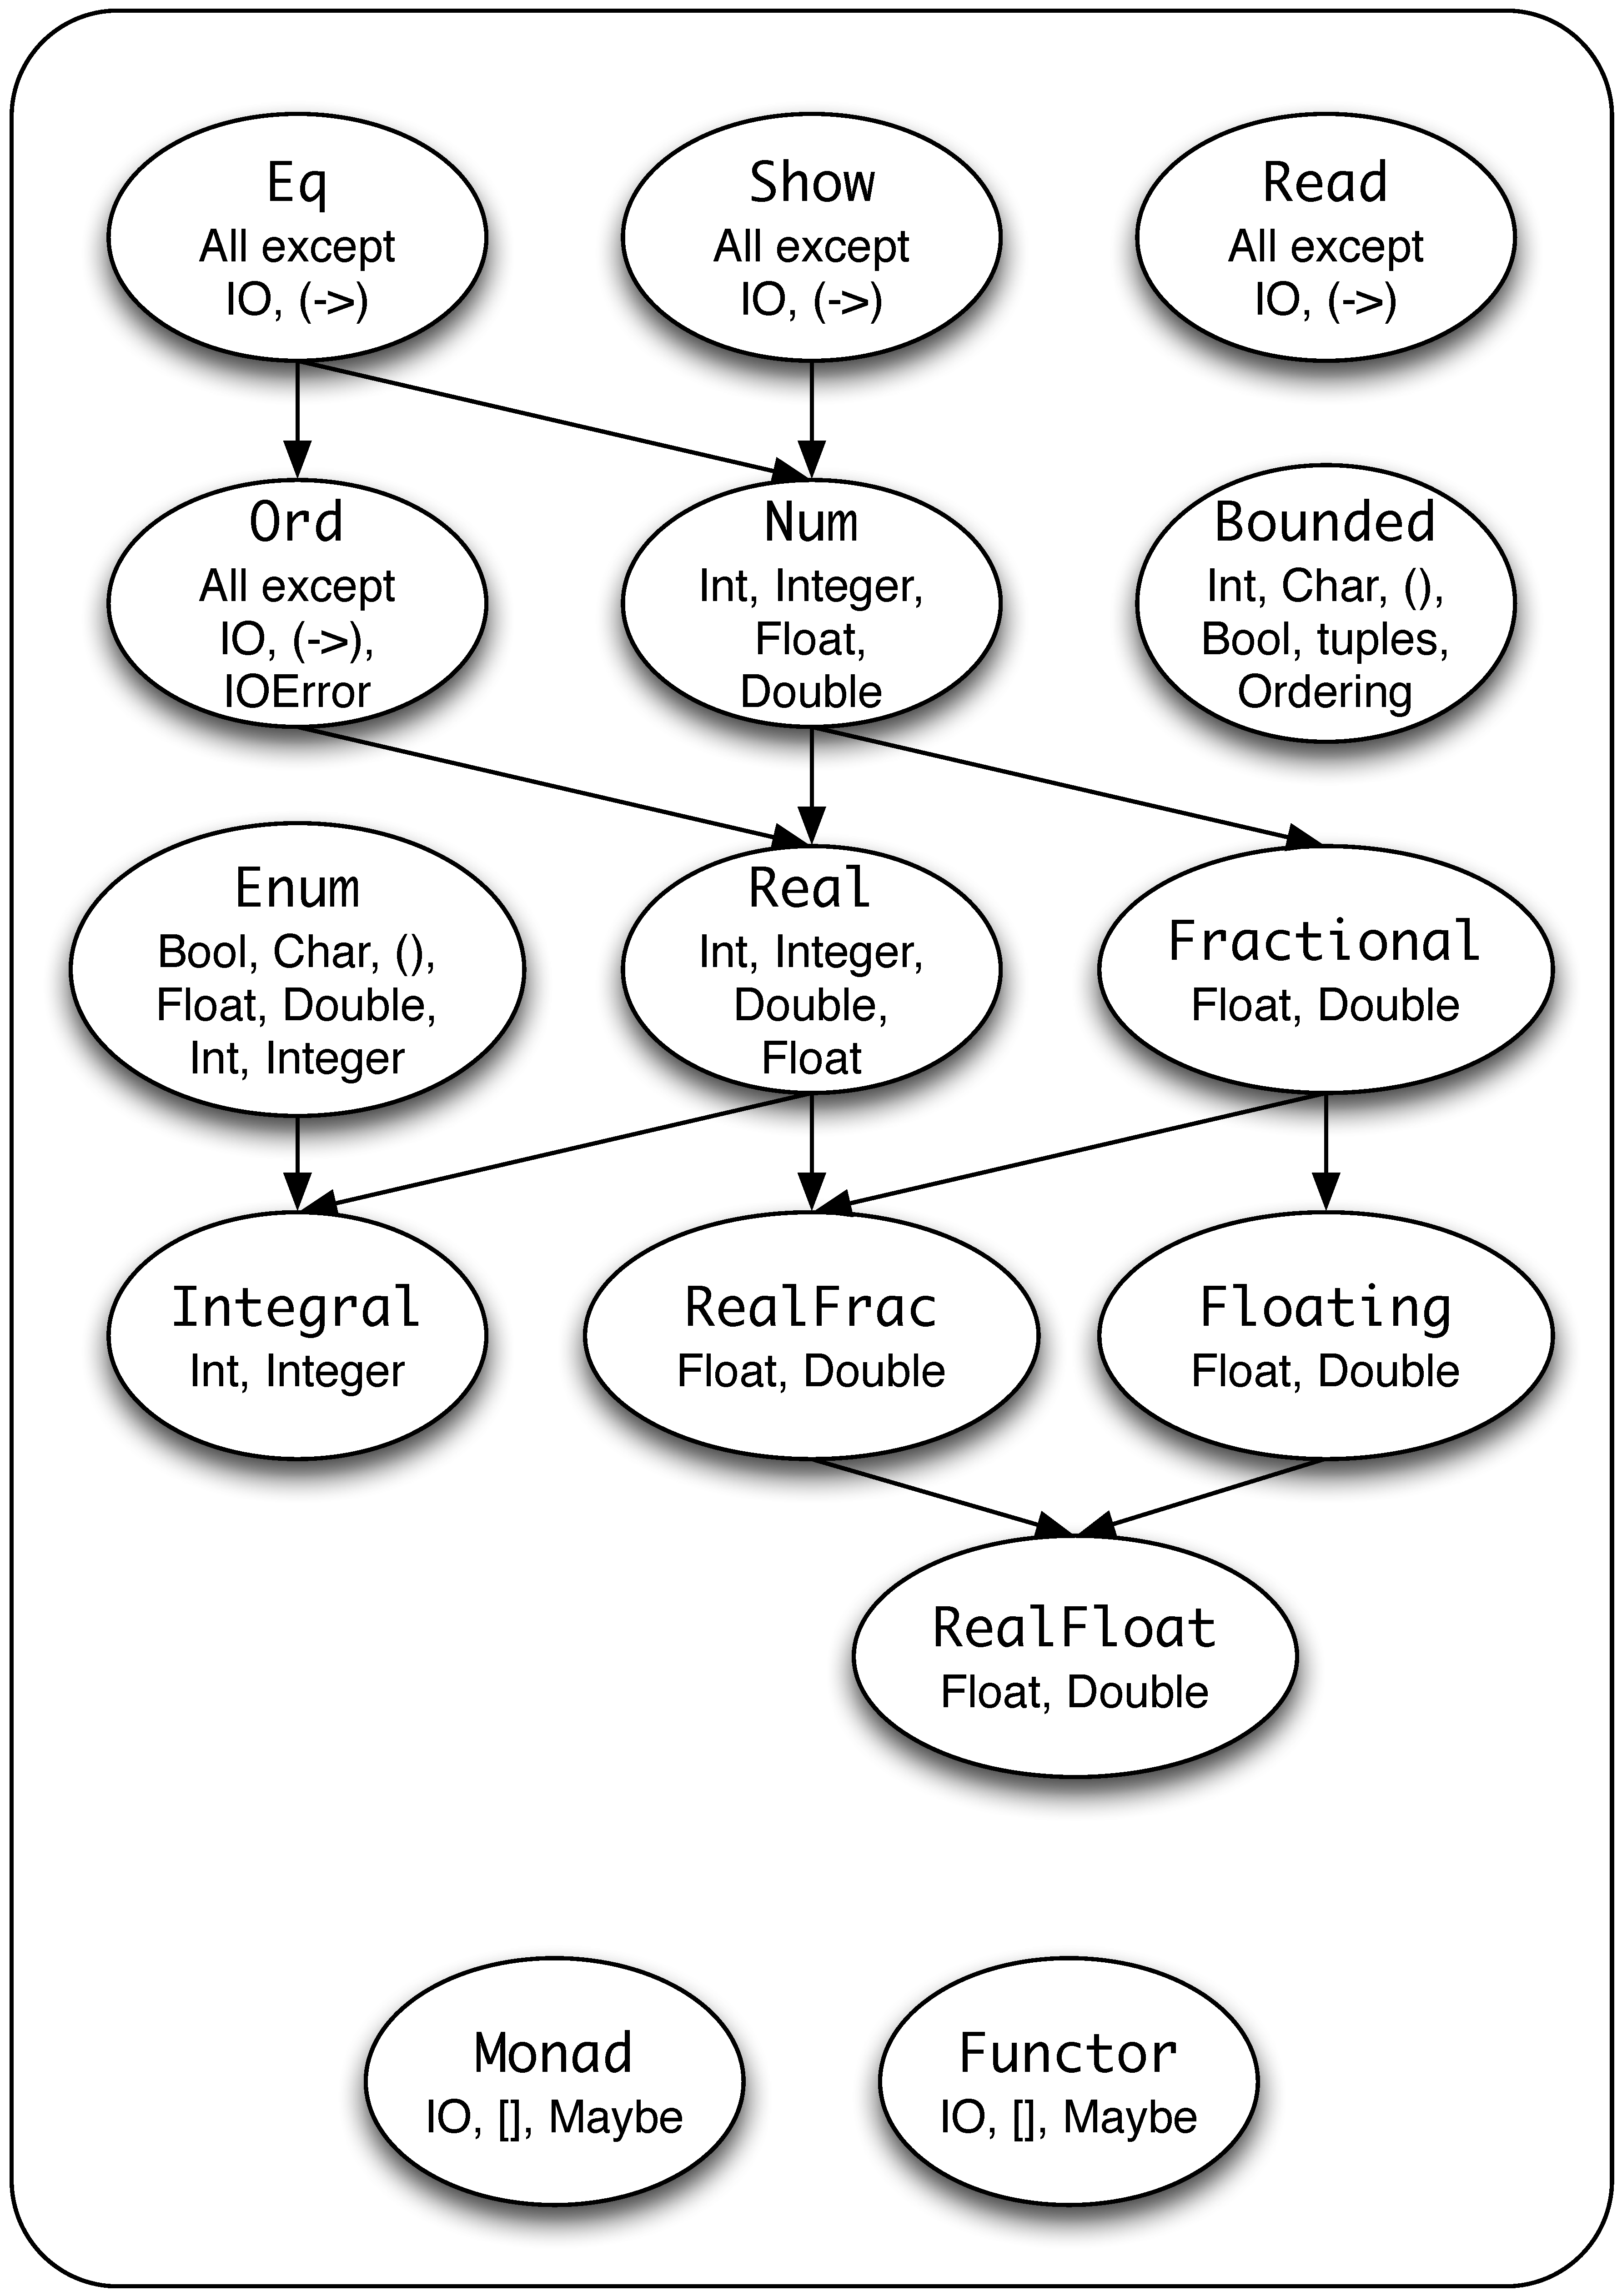
\includegraphics[width=3.5in]{Pictures/Classes.pdf}
\end{center}
\caption{The Haskell 2010 classes}
\label{ClassesDiagram}\index{Haskell 2010!classes diagram}\index{classes!diagram for Haskell 2010}
\end{figure}



Finally we have default definitions for the maximum and minimum
operations,
\begin{alltt}\minx{max}\minx{min}
  max x y 
    | x <= y      = y
    | otherwise   = x
  min x y 
    | x <= y      = x
    | otherwise   = y
\end{alltt}
Most Haskell types belong to these equality and ordering classes: among the exceptions
are function types, and some of the abstract data types we meet below in
Chapter \ref{adt}.

\subsection*{Enumeration: \texttt{Enum}}

It is useful to generate lists like \texttt{[2,4,6,8]} using the enumeration
expression
\begin{alltt}
[2,4 ..\ 8]
\end{alltt}
but enumerations can be built over other types as well: characters, floating-point numbers, and so on. The class definition is 
\begin{alltt}
class (Ord a) => Enum a where\minx{Enum}\minx{toEnum}\minx{fromEnum}
  succ, pred       :: a -> a
  toEnum           :: Int -> a
  fromEnum         :: a -> Int
  enumFrom         :: a -> [a]              -- [n ..\ ]
  enumFromThen     :: a -> a -> [a]         -- [n,m ..\ ]
  enumFromTo       :: a -> a -> [a]         -- [n ..\ m]
  enumFromThenTo   :: a -> a -> a -> [a]    -- [n,n' ..\ m]
\end{alltt}
where \texttt{enumFromTo} and \texttt{enumFromThenTo} have default definitions,
which we leave as exercises for the reader. 

The signature of the class also contains operations \texttt{fromEnum} and
\texttt{toEnum} which convert
between the type and \texttt{Int}. Finally, the class contains \texttt{succ} and \texttt{pred} which step through the enumeration upwards and downwards: when \texttt{succ} is called at the greatest element, an error is returned. 

Confusingly, the Haskell report
states that `these functions [\texttt{toEnum} and \texttt{fromEnum}] are 
not meaningful for all instances of
\texttt{Enum}', and using these operations over floating-point values or 
full precision integers will result in a run-time error.

Full instances of the class include \texttt{Int}, \texttt{Char},
\texttt{Bool} and other finite types like \texttt{Ordering}. 

\subsection*{Bounded types: \texttt{Bounded}}\minx{Bounded}
\minx{minBound}\minx{maxBound}
The \texttt{Bounded} class is specified by the declaration
\begin{alltt}
class Bounded a where
  minBound, maxBound :: a
\end{alltt}
and the two values give the minimum and maximum values in these types.
The types \texttt{Int}, \texttt{Char}, \texttt{Bool}, \texttt{Ordering}
belong to this class. Types that are in both \texttt{Bounded} and \texttt{Enum} obey some extra constraints that are explained in detail in the Haskell 2010 report \cite{haskell2010}.

\subsection*{Turning values to strings: \texttt{Show}}\index{show@\texttt{show}}

The standard prelude defines the class
\texttt{Show}, 
which contains types whose values can be written (or `shown') as strings. 
\begin{alltt}
type ShowS = String -> String

class Show a where
  showsPrec :: Int -> a -> ShowS
  show      :: a -> String
  showList  :: [a] -> ShowS
\end{alltt}
The function \texttt{showsPrec} supports flexible and efficient conversion of large data values, but in an
introductory context, the function
\begin{alltt}
show :: a -> String
\end{alltt}
which converts a value into a string is all that is needed. The class contains default definitions of
\texttt{showsPrec} from \texttt{show} and vice versa. Further details about how to exploit the subtleties of
\texttt{showsPrec} can be found in
\citeN{gentle98}.

Most types belong to the class \texttt{Show}, but absent are function types and \texttt{IO}. For other types, example instance declarations might be
\begin{alltt}
instance Show Bool where
   show True  = "True"
   show False = "False"

instance (Show a, Show b) => Show (a,b) where
   show (x,y) = "(" ++ show x ++ "," ++ show y ++ ")"
\end{alltt}
In fact we discuss how some function types might be shown in Section \ref{qcGens}.


\subsection*{Turning strings to values: \texttt{Read}}

The class \texttt{Read}\minx{Read}
contains types whose values can be read from
strings. To use the class it is enough to know about the function
\begin{alltt}
read :: (Read a) => String -> a\minx{Read}\minx{read}
\end{alltt}
The result of a
\texttt{read} may not be properly defined: there needs to be exactly one object
of the required type in the input string (which may optionally also contain
whitespace or nested
comments); in any other case the \texttt{read} will fail with an error. More
details of how strings are \textbf{parsed} in this way can be found in Section
\ref{parsing}.

It is also important to see that
in many cases the type of the result of the \texttt{read} has to be
specified, since it could potentially be of any type in the class \texttt{Read}.
For instance, we can write
\begin{alltt}
(read " 1 ") :: Int
\end{alltt}
which indicates
that in this case we require the result of the \texttt{read} to be
an \texttt{Int}. Without this type declaration we get this error on evaluating \texttt{(read " 1 ")}:
\begin{alltt}
Ambiguous type variable `a' in the constraint:
  `Read a' arising from a use of `read' at <interactive>:1:0-8
Probable fix: add a type signature that fixes these type variable(s)
\end{alltt}
The class \texttt{Read} complements \texttt{Show}, since strings produced
by \texttt{show} are usually readable by \texttt{read}. Many types can be read, but
exclusions include function types.

\subsection*{The Haskell numeric types and classes}

\index{type!numeric types|(}\index{classes!numeric|(}\minx{Int}\minx{Float}
One of the purposes of the Haskell
design was to build a functional programming language
which had a strong type system -- in which any type errors in definitions and
expressions are found before evaluation -- yet which contains a rich set of
numeric types, as befits a language suitable to substantial `real world' tasks.
Among Haskell's numeric types are 
\begin{titemize} 
\item The fixed precision integers, \texttt{Int}, and the full precision
integers, \texttt{Integer}, which represent {\em all\/} integers faithfully.
\item The floating-point numbers, \texttt{Float}, and the double-precision
floating-point numbers, \texttt{Double}.
\item Rational numbers, that is fractions, represented as ratios of integers;
built-in is the type \texttt{Rational} of \texttt{Integer} fractions.
\item Complex numbers, which can be built over other types such as 
\texttt{Float}.
\end{titemize}
The design also required that the usual operations like \texttt{+} and \texttt{/}
and literals such as \texttt{23} and \texttt{57.4} would be overloaded. For
instance, \texttt{Int} and \texttt{Integer} will carry identical
operations\footnote{Apart from (de)coding of {\smtt Char}, \texttt{take}, \texttt{drop}
and so forth.} and have
identical literals, as indeed will \texttt{Float} and \texttt{Double}; a guide to
the operations over integers and floats was given in Sections \ref{ints} and
\ref{float}. This
overloading can lead to situations  where the type of an expression is
undetermined; in such a case we can give an explicit type to an expression,
thus:
\begin{alltt}
(2+3)::Int
\end{alltt}
The Haskell report \cite{haskell2010}, Section 4.3.4, discusses a mechanism by which
a \emph{default} type can be given to numeric expressions.\label{ambiguity} These default directives mean that whole numbers are taken to be \texttt{Integer} and others to be \texttt{Double} in the absence of any other type information. This can be seen in action in this snapshot of GHCi:
\begin{alltt}
\textsl{Prelude>} let myadd = (+)
\textsl{Prelude>} :type myadd
\textsl{myadd :: Integer -> Integer -> Integer}
\end{alltt}
Overloading of numeric functions is achieved by defining a collection of classes. 
Full details of
these can be found in the Haskell report \cite{haskell2010}, and in the standard
prelude, \texttt{Prelude.hs}\minx{Prelude.hs}; a
brief introduction follows here.

The base class to which all numeric types belong is \texttt{Num}\minx{Num}, which
has the signature\index{numbers!\texttt{Num}}\minx{-}
\begin{alltt}\minx{+}\minx{*}\minx{Eq}\minx{Show}
class (Eq a, Show a) => Num a where
  (+), (-), (*)  :: a -> a -> a
  negate         :: a -> a\minx{negate}
  abs, signum    :: a -> a\minx{abs}\minx{signum}
  fromInteger    :: Integer -> a\minx{fromInteger}

  x - y           = x + negate y
\end{alltt}
This signature has the effect that all numeric types carry 
equality and \texttt{show} functions, together
with addition, subtraction, multiplication and related operations. It is
also possible to convert an \texttt{Int} or and \texttt{Integer} into a
value of any numeric type.

Integer literals are of any numeric type, so that, for
example\index{numbers!integer literals}\index{overloaded
literals!integer}
\begin{alltt}
2 :: Num a => a
\end{alltt}
The integer types belong to the class \texttt{Integral}\minx{Integral}
among whose signature functions are\index{numbers!\texttt{Integral}}
\begin{alltt}\minx{quot}\minx{rem}\minx{div}\minx{mod}
quot, rem :: a -> a -> a
div, mod  :: a -> a -> a
\end{alltt}
which give two variants of integer division, \texttt{`quot`} truncating
towards zero, and \texttt{`div`} truncating below.

Numbers with fractional parts have a substantially richer class structure. 
Literals of this kind belong to every type in the \texttt{Fractional}
class,
\begin{alltt}\minx{Fractional}\index{numbers!\texttt{Fractional}}
2.3 :: Fractional a => a 
\end{alltt}
which extends \texttt{Num} with fractional division and reciprocal,
\begin{alltt}\minx{/}\minx{recip}
class (Num a) => Fractional a where
  (/)          :: a -> a -> a
  recip        :: a -> a
  fromRational :: Rational -> a

  recip x       = 1 / x
\end{alltt}
The floating-point numbers in \texttt{Float}\minx{Float} and \texttt{Double}\minx{Double} 
belong to the class
\texttt{Floating}, which carries the `mathematical' functions. A part of
its signature follows, \index{floating-point
operators}\index{numbers!floating-point}
\begin{alltt}\minx{Floating}
class (Fractional a) => Floating a where
  pi                  :: a\minx{pi}
  exp, log, sqrt      :: a -> a\minx{exp}\minx{log}\minx{sqrt}
  (**), logBase       :: a -> a -> a\minx{**}\minx{logBase}
  sin, cos, tan       :: a -> a\minx{sin}\minx{cos}\minx{tan}
   ....
\end{alltt}
and the full signature is to be found in \texttt{Prelude.hs}. Further
details of this and 
the complex and rational types can be found in the prelude, libraries and the
Haskell documentation.
\index{classes!numeric|)}
\index{type!numeric types|)}


\subsection*{Derived instances}\index{instance!derived}

When a new \texttt{data} type is introduced, it comes with facilities for pattern matching but no other pre-defined functions. On the other hand, it's possible to come up with standard definitions of equality, ordering, \texttt{show} and \texttt{read} functions for these types, and this \textbf{deriving} mechanism is the bit of `Haskell magic' which we mentioned in Sections \ref{EnumTypes} and \ref{introAlg} when we introduced \texttt{data} type definitions. If we make a definition like
\begin{alltt}\minx{People}
data People = Person Name Age
              deriving (Eq,Show)
\end{alltt}
then definitions of \texttt{==} and \texttt{show} which ``do the obvious thing'' are synthesised for this type. This could be done for all the standard classes, but we could  also choose to define instances of other standard classes for ourselves, so that we might read name, age pairs from a comma separated variable (CSV) file, rather than using the standard definition of \texttt{read}, which would expect input of the form
\begin{alltt}
Person "name" age
\end{alltt}

\beware{\texttt{Functor} and \texttt{Monad}}{
We talk about the \texttt{Functor} and \texttt{Monad} classes in Chapter \ref{actions}.
}


\begin{exercises}
 

\item
Investigate the Haskell definition of `\texttt{<}' on the types \texttt{Bool} and
\texttt{(\tone,\ttwo,\ldots,\subscr{t}{k})}.

\item
Define a function
\begin{alltt}
showBoolFun :: (Bool -> Bool) -> String
\end{alltt}
which displays a Boolean function as a table. Generalize this to
\begin{alltt}
showBoolFunGen :: (a -> String) -> (Bool -> a) -> String
\end{alltt}
whose first argument is a
function to show elements of \texttt{a}. This argument is used in giving a table
of the results of the function. How would you extend your answer to deal
with multiple-argument Boolean functions?

\item
Using your answer to the previous question, or otherwise, describe how
you would make \texttt{Bool -> Bool} an instance of the class
\texttt{Show}. (Note, however, that this will {\em not\/} be legitimate Haskell 2010,
since \texttt{Bool -> Bool} is not of the right form for an instance
declaration; you \emph{can} achieve this using the GHC option \texttt{-XFlexibleInstances}.)

\item
How can you write a general instance for \texttt{Show} for function types: you could do this by showing a ``sample'' of the values from the function, that is showing how a sample of inputs are sent to the corresponding outputs.

\item
Some types are not enumerated in the sense that they can be listed from smallest to largest: a good example is the \texttt{Move} type from the Rock - Paper - Scissors game. Define a type class to which the \texttt{Move} type can belong, and give an instance for \texttt{Move}. What other types can you think of giving an instance for: give some examples and their instances, too.

\item
Define a \texttt{data} type \texttt{Roman} like this
\begin{alltt}
data Roman = Roman Integer
\end{alltt}
and define instances of \texttt{Show} and \texttt{Num} for this type. The \texttt{show} function should display numbers in the form of Roman numerals, so that
\begin{alltt}
show (Roman 99) = "IC"
show (Roman 1327) = "MCCCXXVII"
\end{alltt}
and so forth. The instance of \texttt{Num} should obey
\begin{alltt}
(Roman n) + (Roman m) \step{} Roman (n+m)
\end{alltt}

\item {[Harder]}
For the \texttt{data} type \texttt{Roman} define an instances of the \texttt{Read} class, which is the inverse of the \texttt{show} function in the previous question.



\end{exercises}



\beware{Type classes and object-oriented programming}{
\label{advClasses}
\index{classes!and OO programming}
This note discusses the relationship between Haskell type classes and the
classes of object-oriented programming; it can be omitted on first reading.

\medskip
The type system of Haskell can be seen as giving monomorphic types to 
functions. Polymorphic types like
\begin{alltt}
show :: Show a => a -> String
\end{alltt}
which involve type classes can be seen as shorthand for 
collections of typings, such as
\begin{alltt}
show :: Bool -> String
show :: Char -> String
\end{alltt}
for each type \texttt{Bool}, \texttt{Char}, \ldots\ belonging to the
class.

In Haskell a class is a collection of types. Other languages such as 
\texttt{C++} make a type and a class the same thing. Under that approach, 
introducing the class of visible
objects would effectively give us a type\footnote{In \texttt{C++} teminology
this would be an abstract base class, with \texttt{Bool} etc. inheriting 
and being forced to implement the
operations of that class.} \texttt{ShowType}. This class would be
characterized by having the function
\begin{alltt}\minx{ShowType}
show :: ShowType -> String
\end{alltt}
in its interface. The class 
\texttt{ShowType}
would have \texttt{Bool} and \texttt{Char} among its sub-classes (or sub-types).
This would allow us
to write values like
\begin{alltt}
[True,'N',False] :: [ShowType]
\end{alltt}
Moreover, to convert such a list to a \texttt{String} we could write
\begin{alltt}
concat . map show :: [ShowType] -> String
\end{alltt}
At different items of the list we use {\em different\/} versions of the 
\texttt{show} function; on the first we use the \texttt{Bool} function, on the second
the \texttt{Char} function and so forth. This so-called \textbf{dynamic binding} is
a powerful feature of many object-oriented languages, including \texttt{C++},
but it is not a feature of
Haskell 98; an extension which would allow dynamic binding is
described in \citeN{extTypes}.

\medskip
Returning to our example, what is the type of \texttt{concat .\ map show} in Haskell? 
It is not hard to see that it is
\begin{alltt}
Show a => [a] -> [Char]
\end{alltt}
so that it can be applied to elements of \texttt{[Bool]}, \texttt{[Char]} and so on,
but not to hetero\-geneous lists like \texttt{[True,'N',False]} which are
not legitimately typed in Haskell.

\medskip
Java allows users to define interfaces, which consist of a signature.
A part of a class definition can say which interfaces the class
implements. This is very like the way in which Haskell types are made
instances of type classes, except that in Haskell it is not necessary to
make the instance declaration a part of the type definition itself. This
has the effect of allowing {\em post hoc\/} extensions to the operations
supported by a type, in a way which is not possible for a class in Java.}

\index{classes|)}


\section{Type checking and type inference: an overview}
\index{type checking|(}

Now that we have covered classes, we can see that every value in Haskell has a defined type, 
which might be monomorphic, polymorphic, or involve one or more type class 
constraints in a context. For example,
\begin{alltt}
'w'   :: Char
flip  :: (a -> b -> c) -> (b -> a -> c)
elem  :: Eq a => a -> [a] -> Bool
\end{alltt}
Strong typing means that we can \textbf{check} whether or
not expressions we
wish to
evaluate or definitions we wish to use obey the typing rules of the
language without any evaluation taking place. The benefit of this is
obvious: we can catch a whole lot of errors before we run a program.



\subsection*{Type declarations or type inference?}\index{type declaration!why to write them}

Haskell types can be \emph{inferred} from expressions and definitions, and so it is possible never to write a type declaration. For example, we can write a definition like this
\begin{alltt}\minx{prodFun}
prodFun f g = \bs{}x -> (f x, g x)
\end{alltt}
either in a module or directly in GHCi, and then ask for its type in CHGi like this:
\begin{alltt}
\textsl{*TypeError>} :type prodFun
\textsl{prodFun :: (t -> t1) -> (t -> t2) -> t -> (t1,t2)}
\end{alltt}
Because of this facility, some Haskellers never write a type declaration, but others, including the author, always do: why?
\begin{itemize}
\item
The type of an object is the \emph{most important single piece of documentation} for the object, since it tells us how it can be used -- what arguments need to be passed to it, and what type the result has -- without us having to understand precisely how it is implemented.
\item
We can use a type declaration to \emph{give a more specific type to a definition}. This was the mechanism underlying the first part of the book, which turned polymorphic functions into monomorphic versions. To be clear, if we define \texttt{prodFun} like this
\begin{alltt}
prodFun :: (Int -> Bool) -> (Int -> Char) -> Int -> (Bool,Char)
prodFun f g = \bs{}x -> (f x, g x)
\end{alltt}
then it will have this more specific type. It is not difficult to recover the most general type for the definition: just comment out the type declaration.
\item
In writing a type declaration we are saying \emph{what type we think a function has}. We may have not got this right, and the function is properly typed, but has a different type. For instance, typing
\begin{alltt}
fun :: Int -> Bool -> Int

fun True 0 = 0
fun True n = n-1
fun _ n    = n\end{alltt}
gives rise to this error in GHCi:
\begin{alltt}
    Couldn't match expected type `Int' against inferred type `Bool'
    In the pattern: True
    In the definition of `fun': fun True 0 = 0
\end{alltt}
In a case like this it is useful to \emph{know} that we were wrong, and then we can either correct the type declaration, or modify the function so that it has the type we wanted. Here the problem is fixed by swapping the types of the two arguments.
\end{itemize}
There is one case where we \emph{do} need to use type declarations or annotations: this is in resolving ambiguity due to overloading (we talked briefly about this earlier, in Section \ref{ambiguity}, page \pageref{ambiguity}).

\subsection*{Types and libraries}


\noindent
Types are also useful in locating functions in a library. Suppose we want to define
a function to remove the duplicate elements from a list, transforming
\texttt{[2,3,2,1,3,4]} to \texttt{[2,3,1,4]}, for instance. Such a
function will have type
\begin{alltt}
(Eq a) => [a] -> [a]
\end{alltt}
A Hoogle search of the standard prelude and libraries reveals just one function of this type, namely
\texttt{nub},\minx{nub} which does exactly what we want. Plainly in practice
there might be multiple matches (or missed matches because of the choice of
parameter order) but nonetheless the types provide a valuable
way into the Haskell library.

\subsection*{Overview}

In the remainder this chapter we give an informal overview of the way in which types
are checked. We start by looking at how type checking works in a
monomorphic framework, in which every properly typed expression has a
single type.
Building on this, we then look at the polymorphic case, and see that it
can be understood by looking at the 
\textbf{constraints}\index{constraint}\index{type checking!constraints} put on the type
of an expression by the way that the expression is constructed. Crucial to this is the
notion of \textbf{unification}, through which constraints are combined.
We conclude the chapter by looking
at the \textbf{contexts} which contain information about the class membership of 
type variables, and which thus manage \textbf{overloading}.

\section{Monomorphic type checking}
\label{monoCheck}
\index{type checking!monomorphic|(}


In this section we look at how type checking works in a monomorphic
setting, without polymorphism or overloading. The main focus here is
type-checking function applications.
The simplified
picture we see here prepares us for Haskell type checking in 
general, which
is examined in the section after this. 

We look first at the way that we type-check expressions, and then look at how definitions 
are type-checked.

\subsection*{Expressions}

In general, an expression is either a literal, a variable or a constant or it 
is built up by applying a function to some
arguments, which are themselves expressions. 

The case of function applications includes
rather more than we might at first expect. For example, we can see list
expressions like \texttt{[True,False]} as the result of applying the
constructor function, `\texttt{:}', thus: \texttt{True:[False]}.
Also, operators and the \texttt{if} \ldots \texttt{then} \ldots \texttt{else}
\index{if@{\texttt{if}\ldots\texttt{then}\ldots\texttt{else}}}\index{operator!type
checking}
construct act in exactly the same way as functions, albeit with a different
syntax.

The rule for type checking a function application is set out in the
following
diagram, where we see that a function of type \texttt{s -> t} must be applied 
to an argument of
type \texttt{s}.
A properly typed application results in an expression of type
\texttt{t}.
\begin{center}
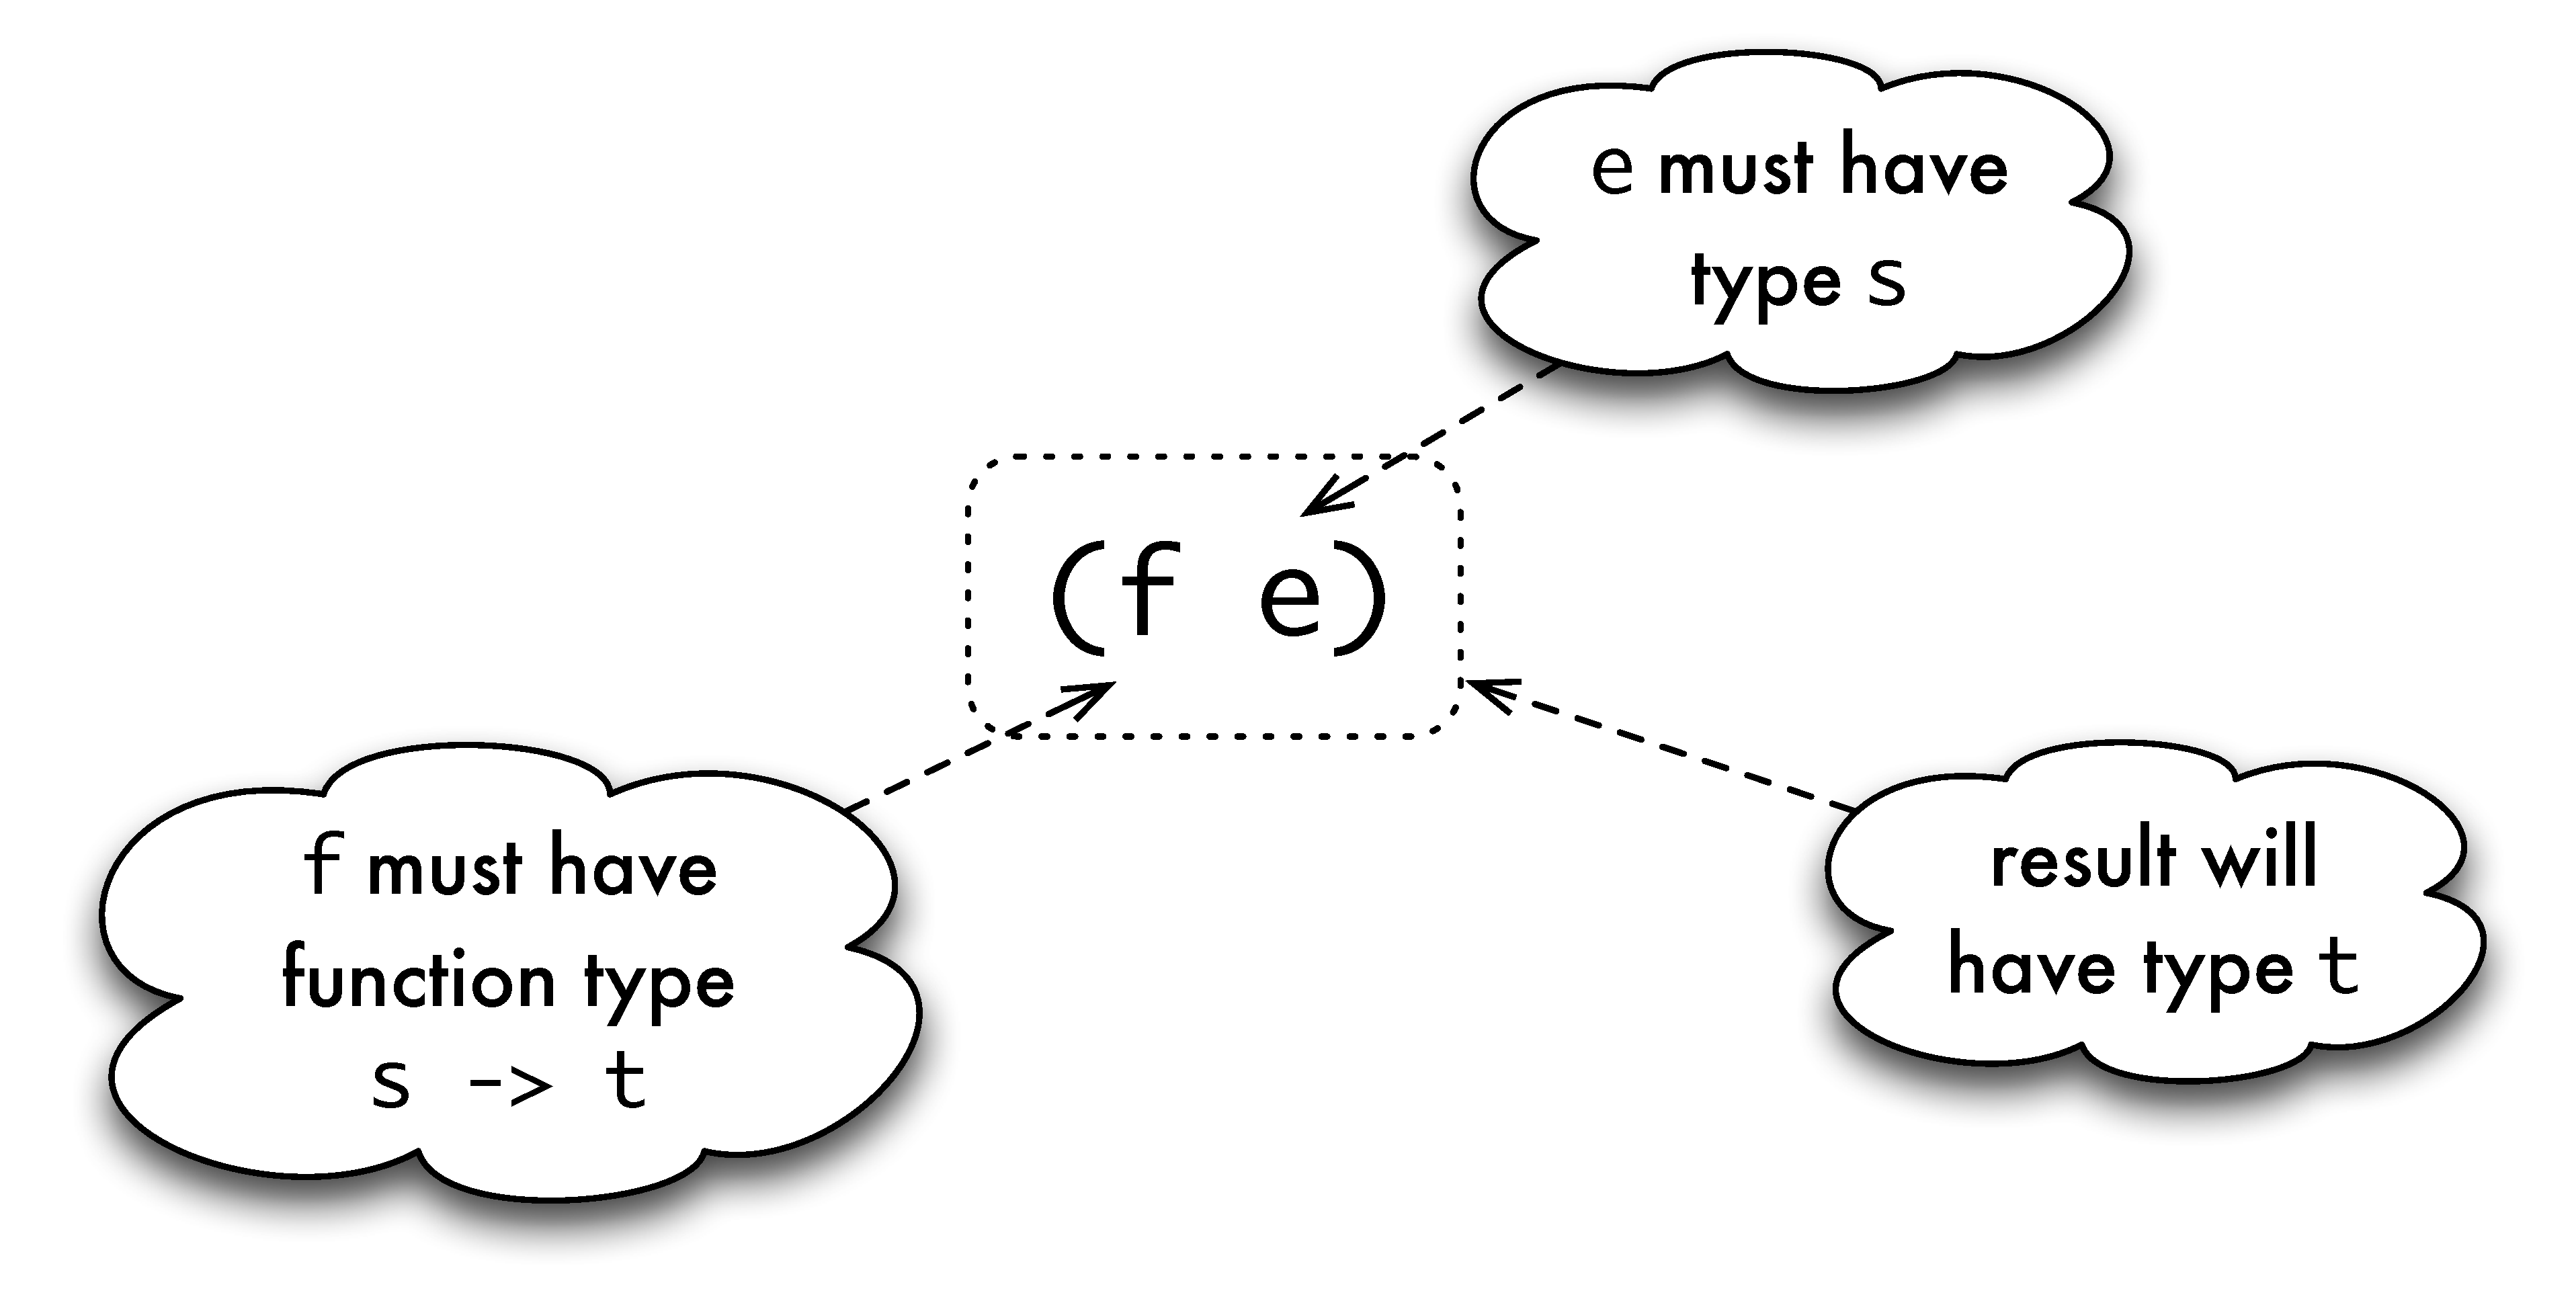
\includegraphics[width=3in]{Pictures/FunctionApp.pdf}
\end{center}
We now look at two examples. First we take \texttt{(not False) \&\& True},
a correctly typed expression of type
\texttt{Bool},
\begin{center}
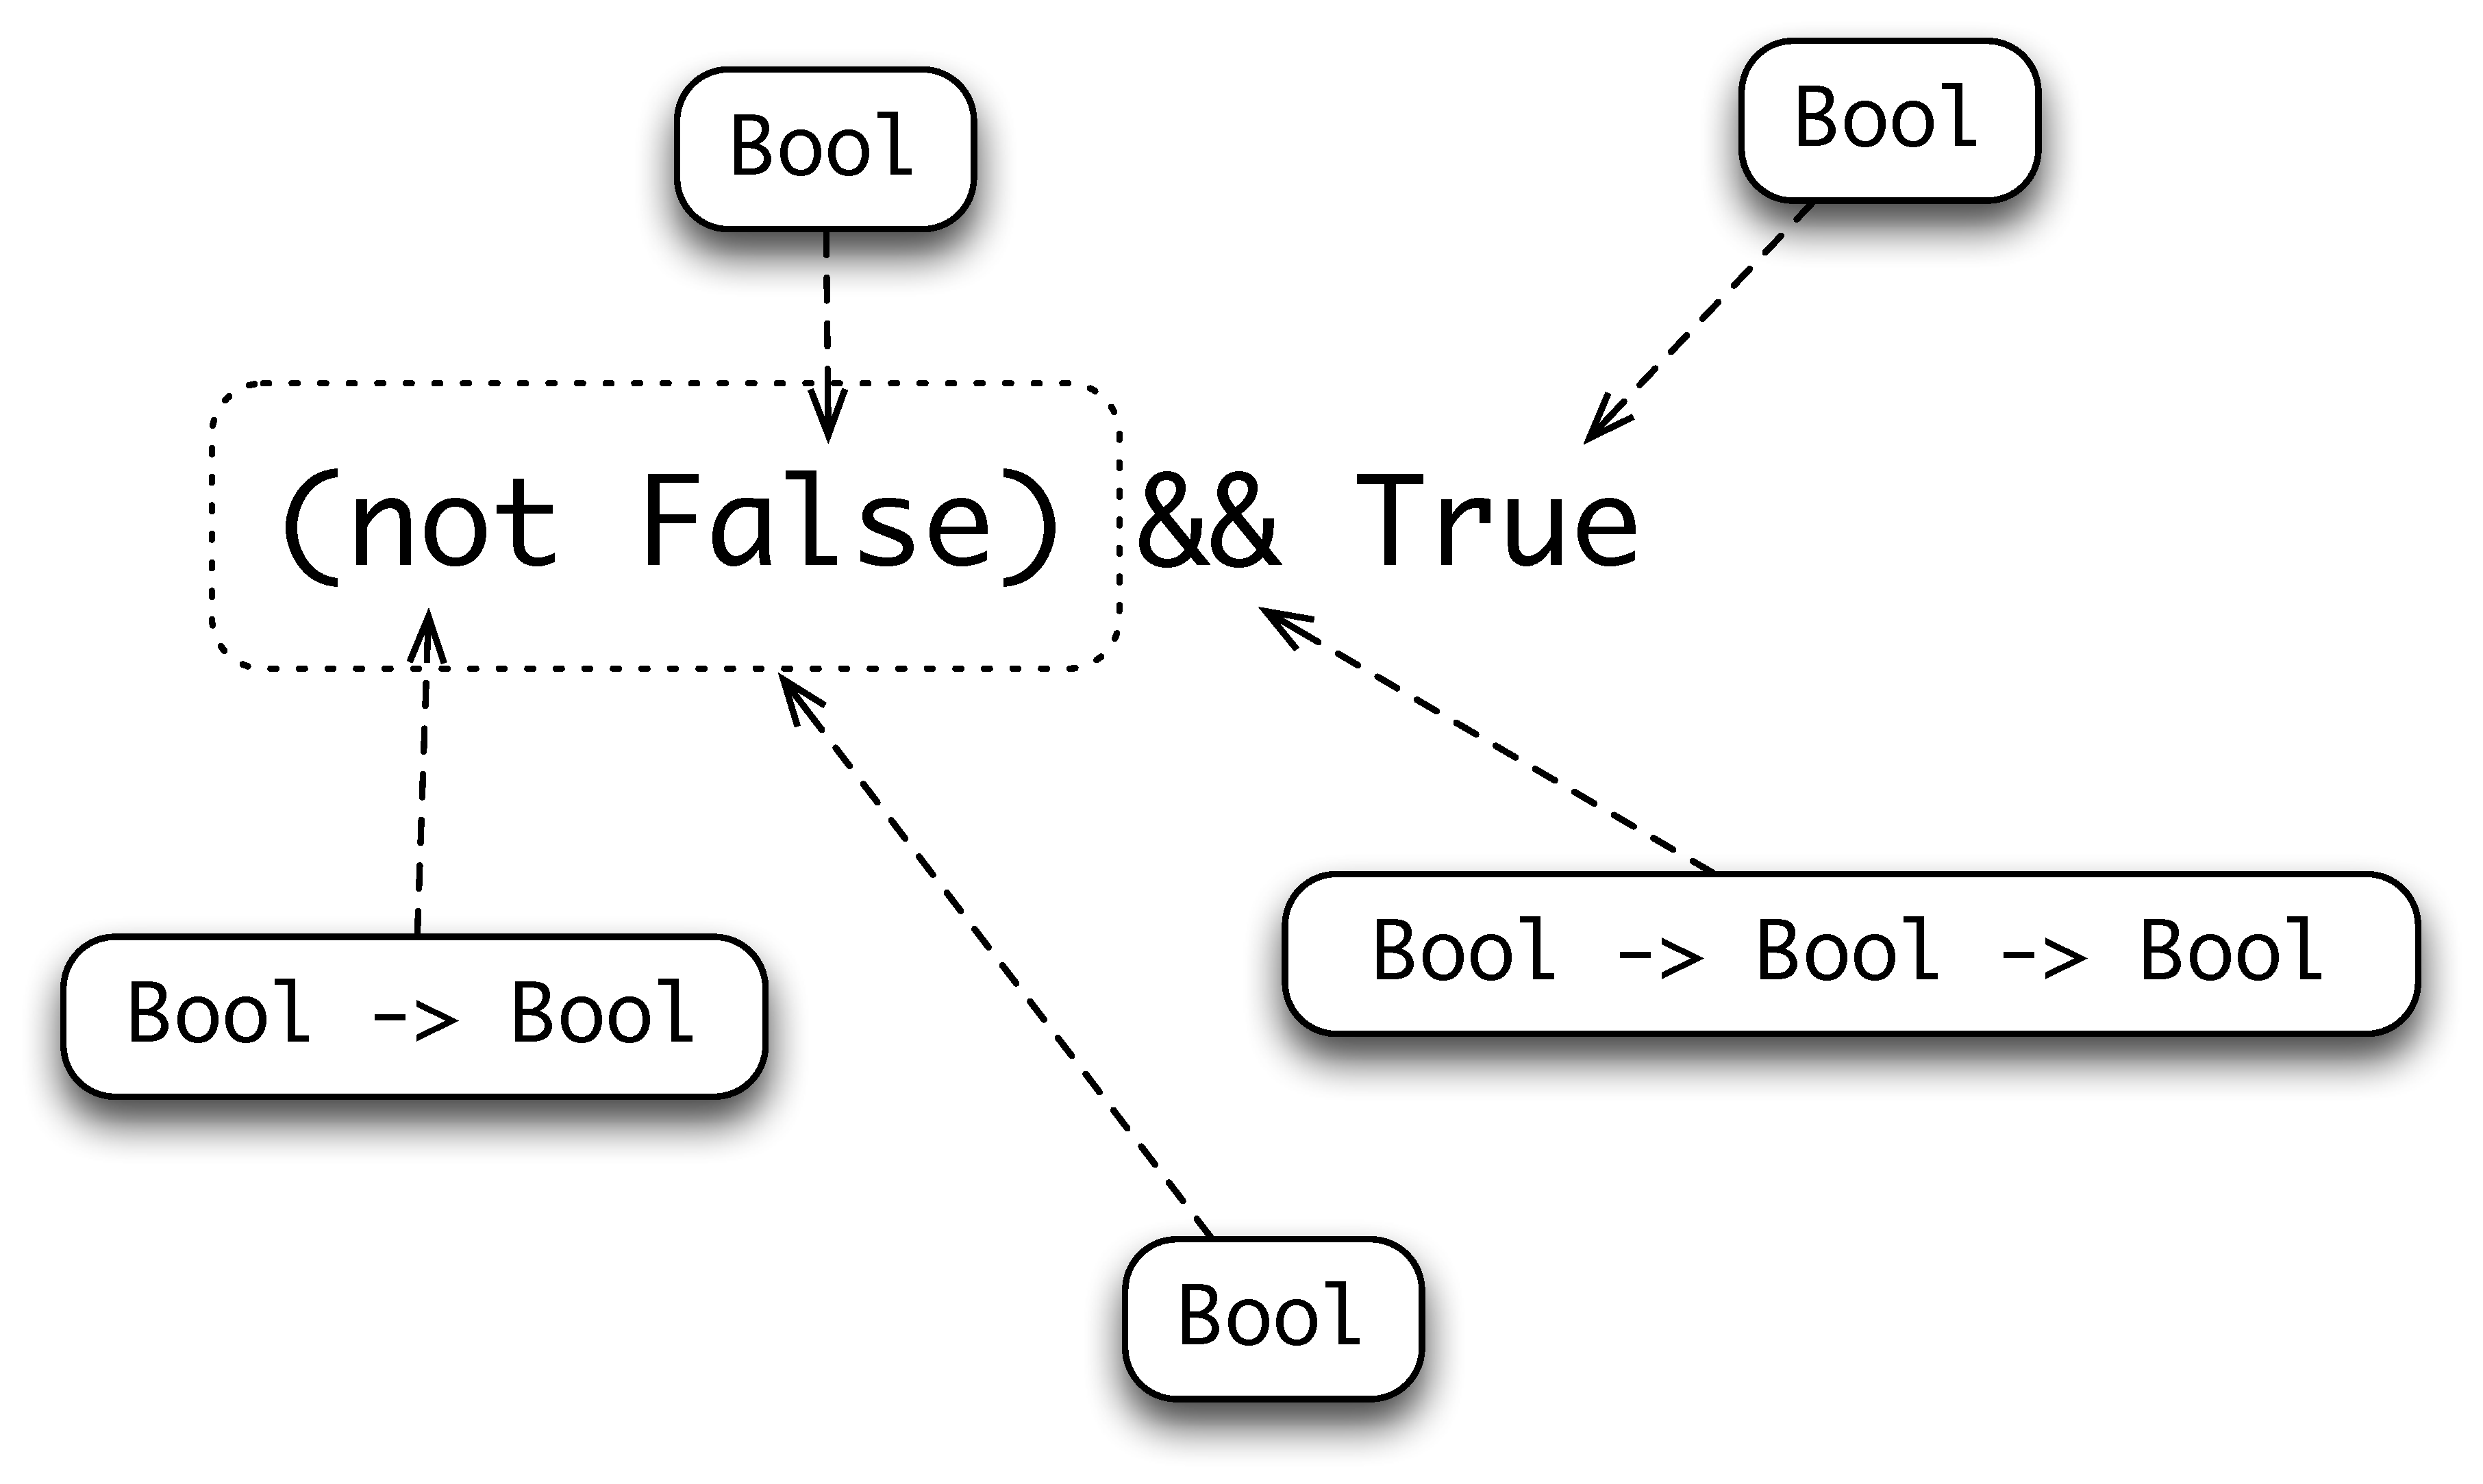
\includegraphics[width=3in]{Pictures/BoolTypeCheck1.pdf}
\end{center}
The application of \texttt{not}\minx{not} to \texttt{False} results in an expression of
type \texttt{Bool}. The second argument to \texttt{\&\&} is also a
\texttt{Bool}, so the application of \texttt{\&\&} is correctly
typed, and gives a result of type \texttt{Bool}.

If we modify the example to \texttt{(not 'c') \&\& True}, we now see a type error, since a character
argument, \texttt{'c'}, is presented to an operator 
expecting\index{type error!in application} a
\texttt{Bool} argument, \texttt{not}.
\begin{center}
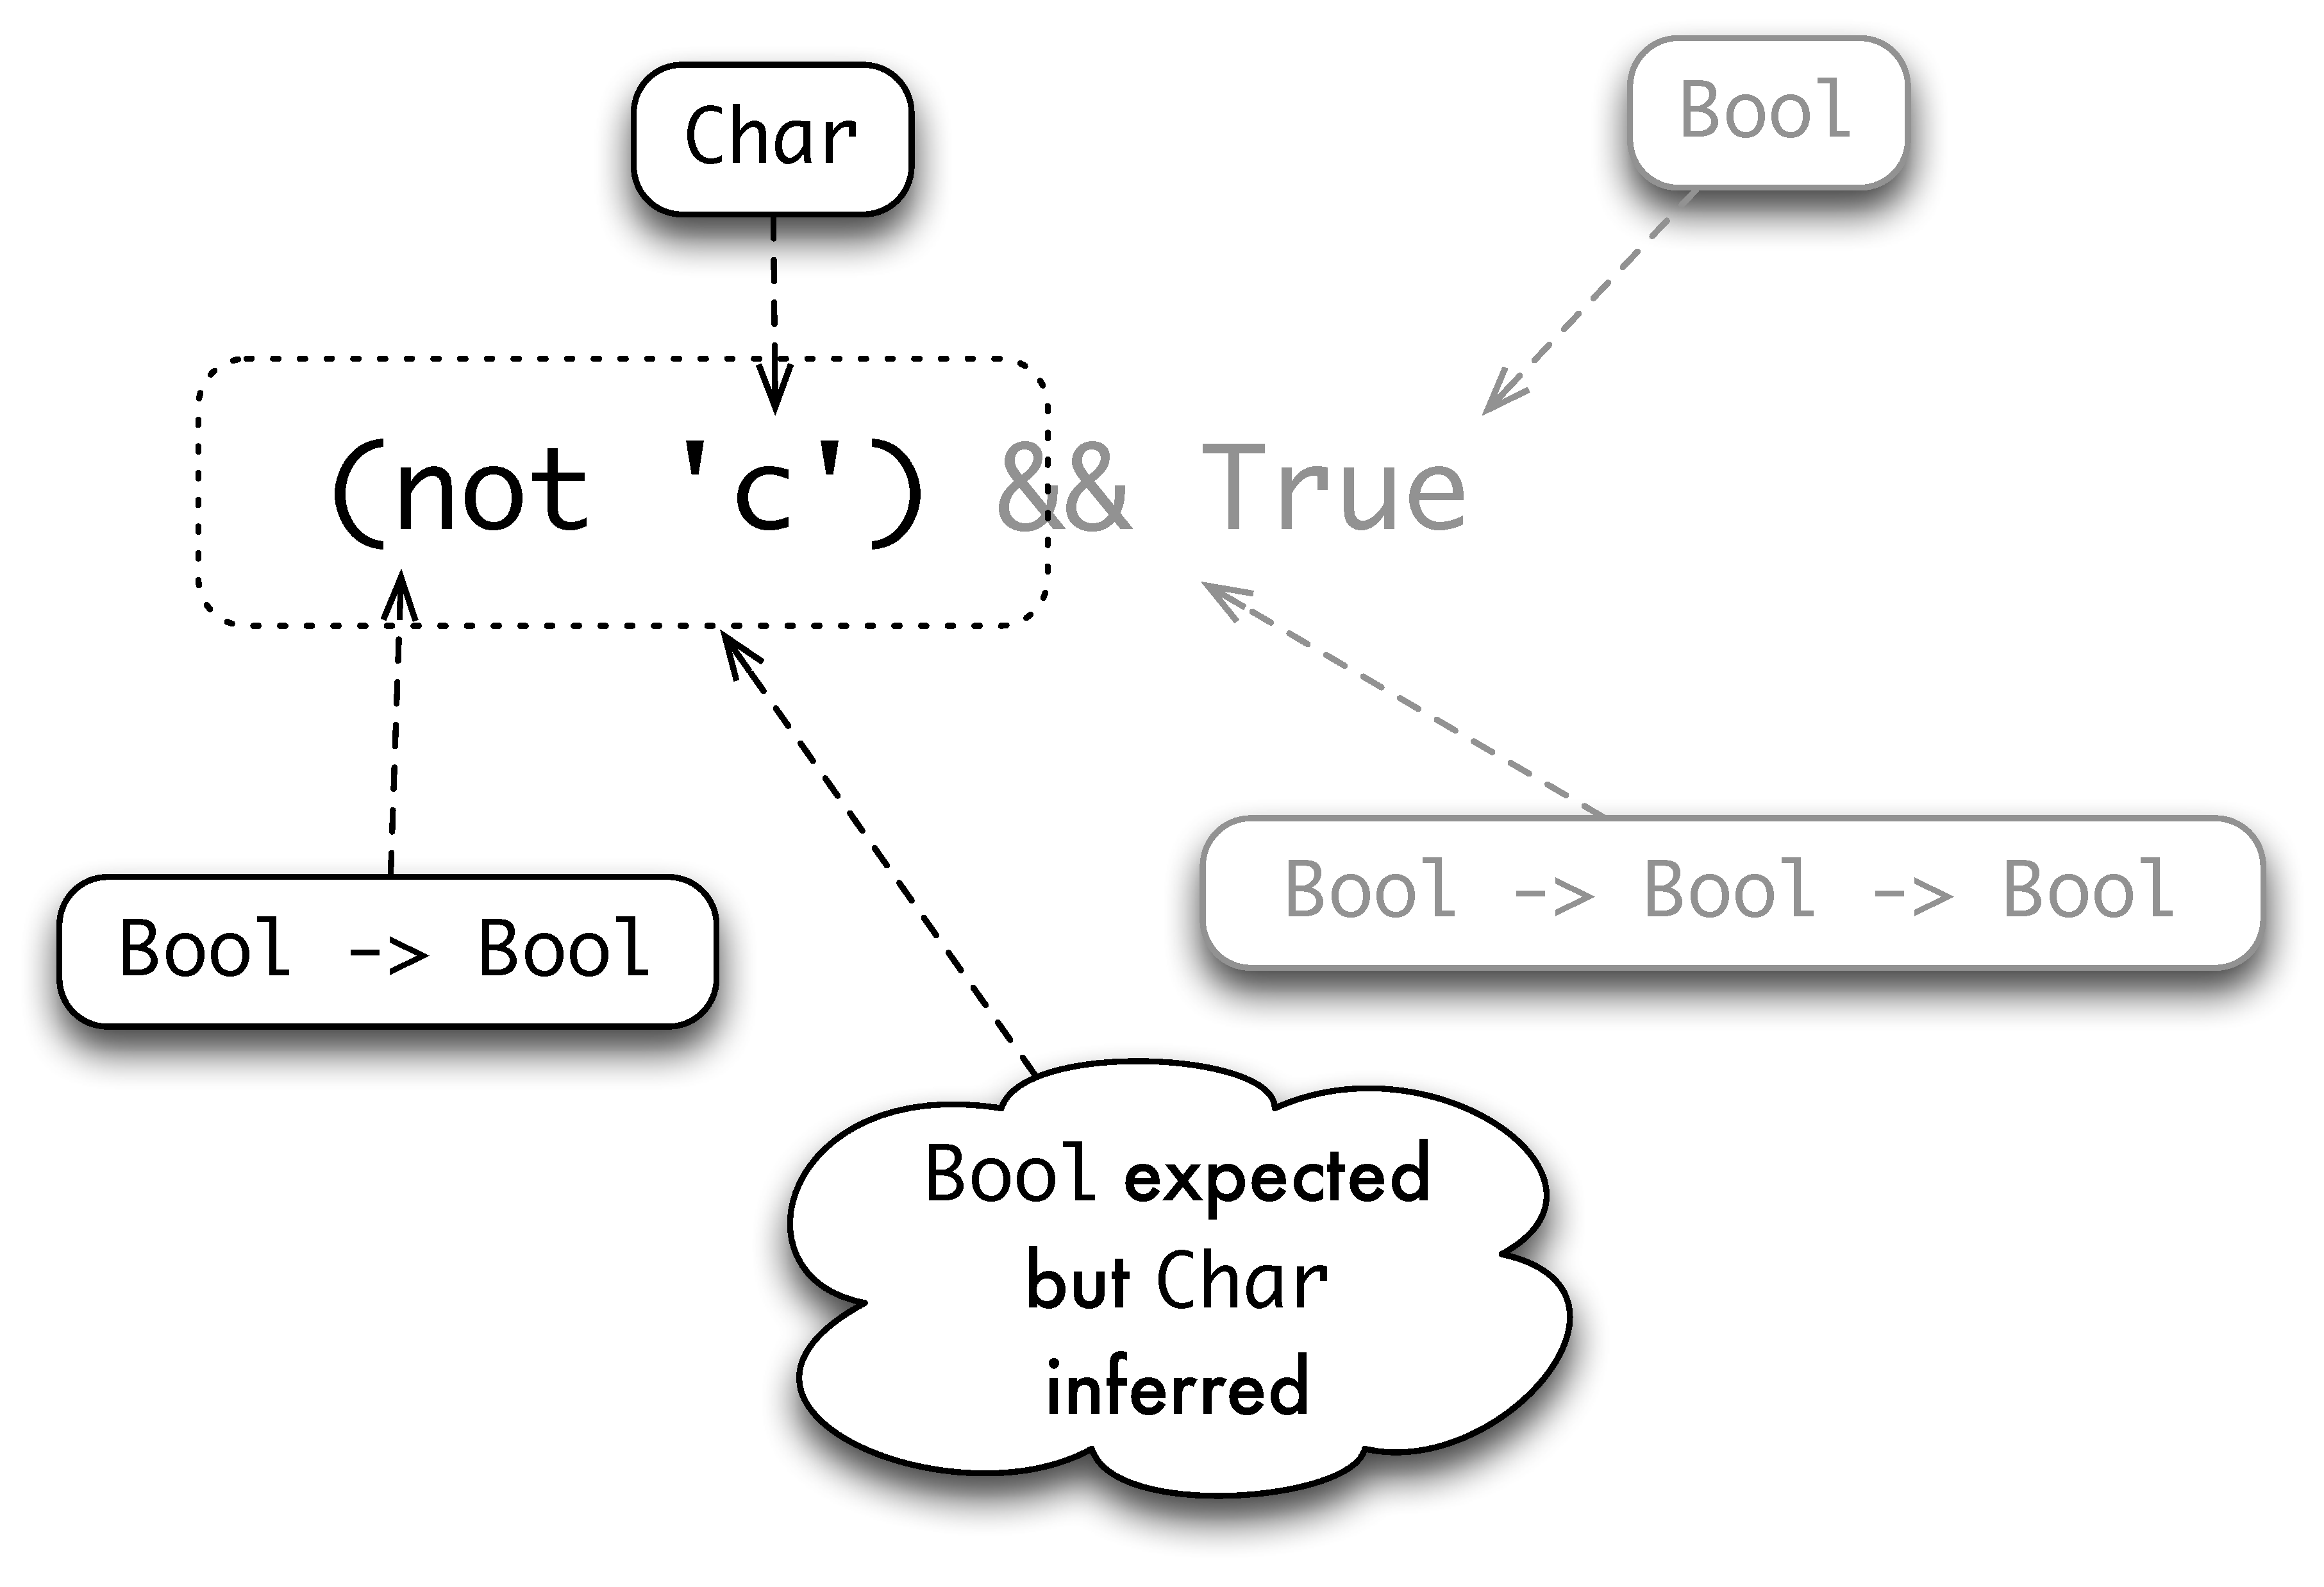
\includegraphics[width=3in]{Pictures/BoolTypeCheck2.pdf}
\end{center}
The GHCi error message for this indicates the cause of the problem:
\begin{alltt}
    Couldn't match expected type `Bool' against inferred type `Char'
    In the first argument of `not', namely 'c'
    In the first argument of `(&&)', namely `(not 'c')'
    In the expression: (not 'c') && True
\end{alltt}

\subsection*{Function definitions}

In type-checking a monomorphic function definition such as 
\begin{alltt}
f :: \smsubscr{t}{1} -> \smsubscr{t}{2} -> \ldots  -> \smsubscr{t}{k} -> t\hfill(fdef)

f \smsubscr{p}{1} \smsubscr{p}{2} \ldots \smsubscr{p}{k}
  | \smsubscr{g}{1}     = \smsubscr{e}{1}
  | \smsubscr{g}{2}     = \smsubscr{e}{2}
  \ldots
  | \smsubscr{g}{l}     = \smsubscr{e}{l}
\end{alltt}
\label{fdef}
we need to check three
things.
\begin{itemize}
\item Each of the guards \smsubscr{g}{i} must be of type \texttt{Bool}.
\item The value \smsubscr{e}{i} returned in each clause must be of type \texttt{t}.
\item The pattern \smsubscr{p}{j} must be consistent with type
of that argument, namely \smsubscr{t}{j}. 
\end{itemize}
A pattern is \textbf{consistent}\index{pattern!consistent with type} with a type if it will match (some) elements of
the type. We now look at the various cases.
A variable is consistent with
any type; a literal is consistent with its type. A pattern \texttt{(p:q)} is consistent with the type
\texttt{[t]} if \texttt{p} is consistent with \texttt{t} and
\texttt{q} is consistent with \texttt{[t]}. For example, \texttt{(0:xs)} is consistent with
the type \texttt{[Int]}, and \texttt{(x:xs)} is consistent with any type
of lists.
The other cases of the
definition are similar. 

This concludes our discussion of type checking in the monomorphic case;
we turn to polymorphism next.


\begin{exerciseone}
\item
Predict the type errors you would obtain by defining the following functions
\begin{alltt}
f n     = 37+n
f True  = 34

g 0 = 37
g n = True

h x 
  | x>0         = True
  | otherwise   = 37

k x = 34
k 0 = 35
\end{alltt}
Check your answers by typing each definition into a Haskell script, and
loading the script into GHCi. Remember that you can use \texttt{:type}
to give the type of an expression.
\index{type checking!monomorphic|)}
\end{exerciseone}

\section{Polymorphic type checking}
\label{polyTypeCheck}
\index{type checking!polymorphic|(}
\index{polymorphism!type checking|(}

In a monomorphic situation, an expression is either well typed, and has
a single type, or is not well typed and has none. In a polymorphic
language like Haskell, the situation is more complicated, since a
polymorphic object is precisely one which has many types. 

In this section we first re-examine what is meant by polymorphism,
before explaining type checking by means of \textbf{constraint satisfaction}.
Central to this is the notion of \textbf{unification}, by which we find
the types simultaneously satisfying two type constraints.


\subsection*{Polymorphism}

We are familiar with functions like
\begin{alltt}
length :: [a] -> Int\hfill(length)
\end{alltt}
whose types are polymorphic, but how should we understand the type
variable \texttt{a} in this type? We can see \texttt{(length)} as
shorthand for saying that \texttt{length} has a \textbf{set} of types,
\begin{alltt}
[Int] -> Int
[(Bool,Char)] -> Int
 ...
\end{alltt}
in fact containing all the types \texttt{[t] -> Int} where \texttt{t} is
a \textbf{monotype},\index{monotype} that is a type not containing type variables.

When we apply \texttt{length} we need to determine at which of these types
\texttt{length}
is being used. For example, when we write
\begin{alltt}
length ['c','d']
\end{alltt}
we can see that \texttt{length}
is being applied to a list of \texttt{Char}, and so we are using
\texttt{length} at type \texttt{[Char] -> Int}.

\subsection*{Constraints}
\index{constraint!in type checking|(}
\index{type checking!constraints|(}

How can we explain what is going on here in general? We can see
different parts of an expression as putting different
\textbf{constraints}
on its type. Under this interpretation, type checking becomes a matter
of working out whether we can find types which meet the constraints.
We have seen some informal examples of this when we discussed the types
of \texttt{map} and \texttt{filter} in Section \ref{hofs}. We consider
some further examples now.

\subsubsection*{Example 1}
Consider the definition
\begin{alltt}
f (x,y) = (x , ['a' .. y])
\end{alltt}
The argument of \texttt{f} is a pair, and we consider separately what
constraints there are on the types of \texttt{x} and \texttt{y}. 
\texttt{x} is completely unconstrained, as it is
returned as the first half of a pair. On the other hand, \texttt{y} is
used
within the expression \texttt{['a' ..\ y]}, which denotes a range within
an enumerated type, starting at the character \texttt{'a'}. This forces
\texttt{y} to have the type \texttt{Char}, and gives the type for
\texttt{f}:
\begin{alltt}
f :: (a,Char) -> (a,[Char])
\end{alltt}

\subsubsection*{Example 2}
Now we examine the definition
\begin{alltt}
g (m,zs) = m + length zs
\end{alltt}
What constraints are placed on the types of \texttt{m} and \texttt{zs} in
this definition? 
We can see that \texttt{m} is added to something, so \texttt{m} must
have a numeric type -- which one it is remains to be seen. The other
argument of the addition is \texttt{length zs}, which tells us two
things. 
\begin{center}
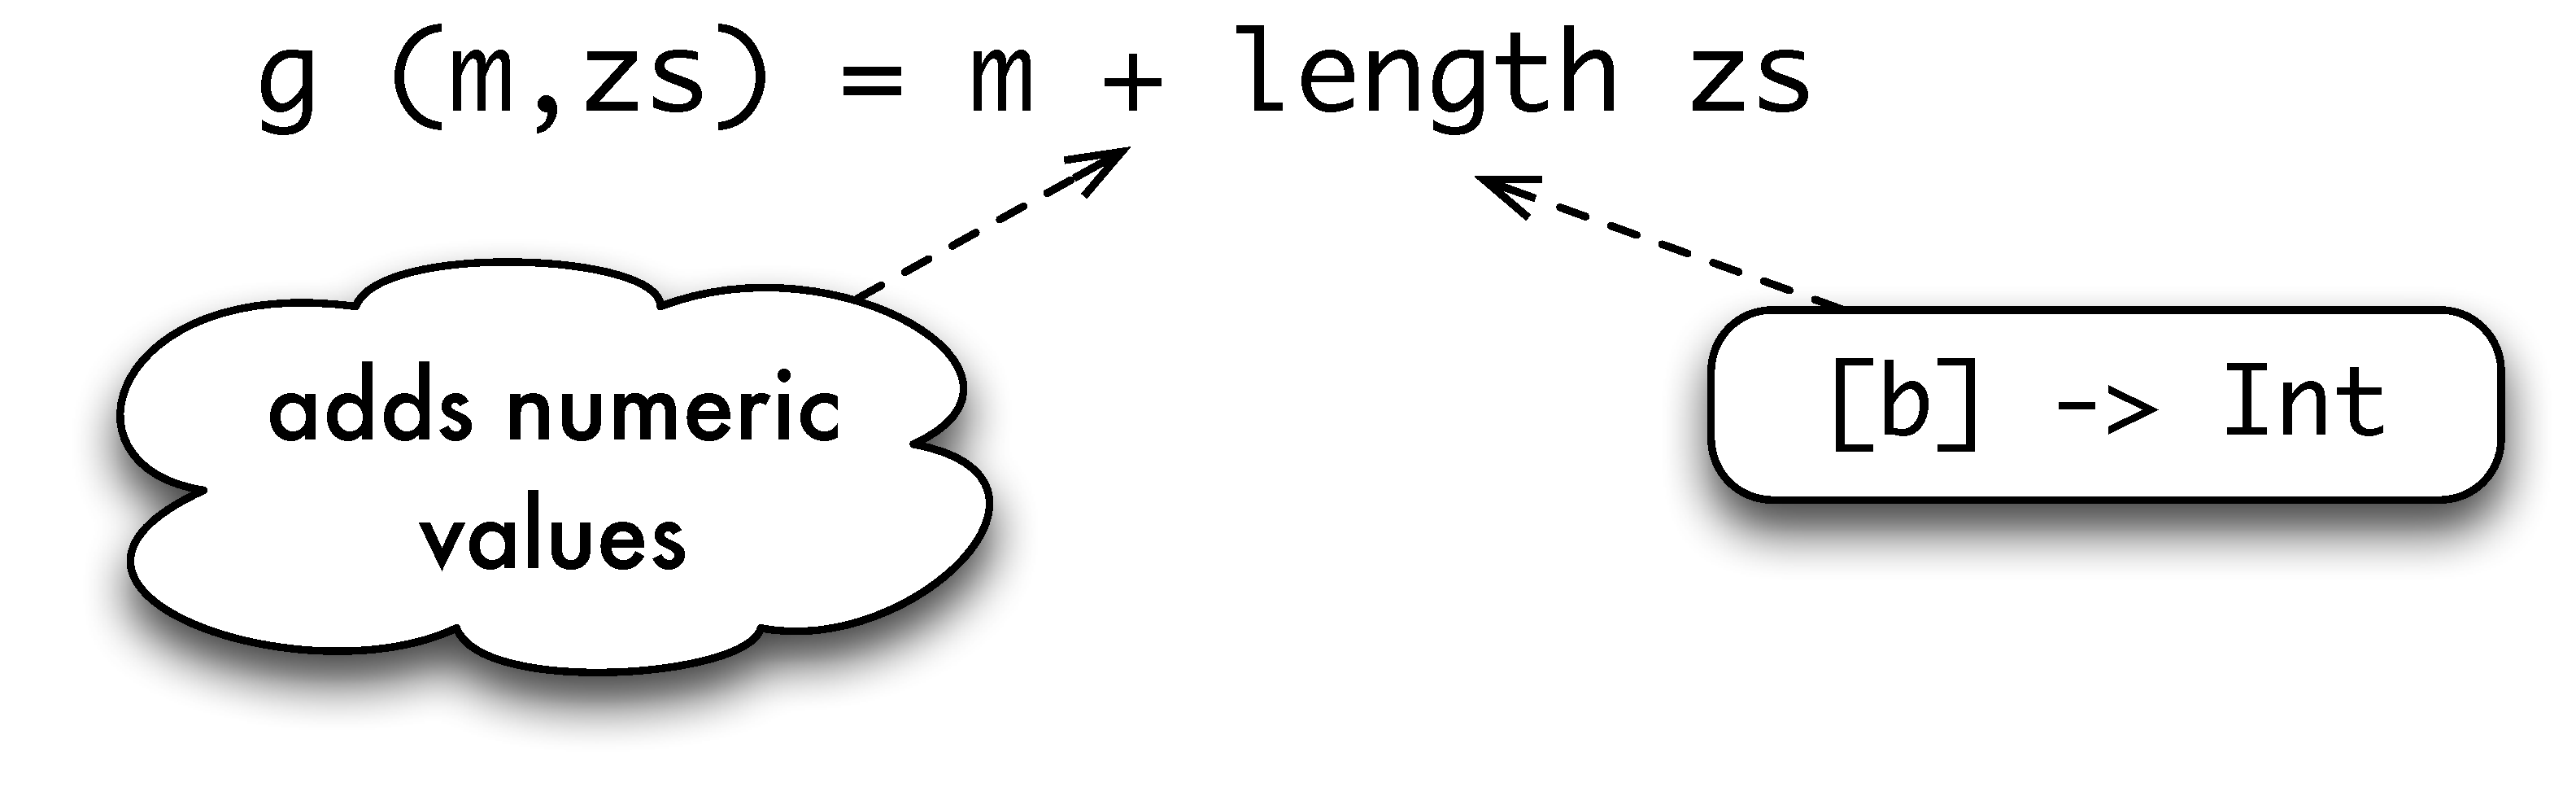
\includegraphics[width=3in]{Pictures/TypeCheckEx2.pdf}
\end{center}
First, we see that \texttt{zs} will have to be of type
\texttt{[b]}, and also that the result is an \texttt{Int}.
This forces \texttt{+} to be used at \texttt{Int}, and so forces
\texttt{m} to have type \texttt{Int}, giving the result
\begin{alltt}
g :: (Int,[b]) -> Int
\end{alltt}

\subsubsection*{Example 3}
\index{function composition}
We now consider the composition of the last two examples,
\begin{alltt}
h = g . f
\end{alltt}
In a composition \texttt{g .\ f}, the output of \texttt{f} becomes
the input of \texttt{g},
\begin{center}
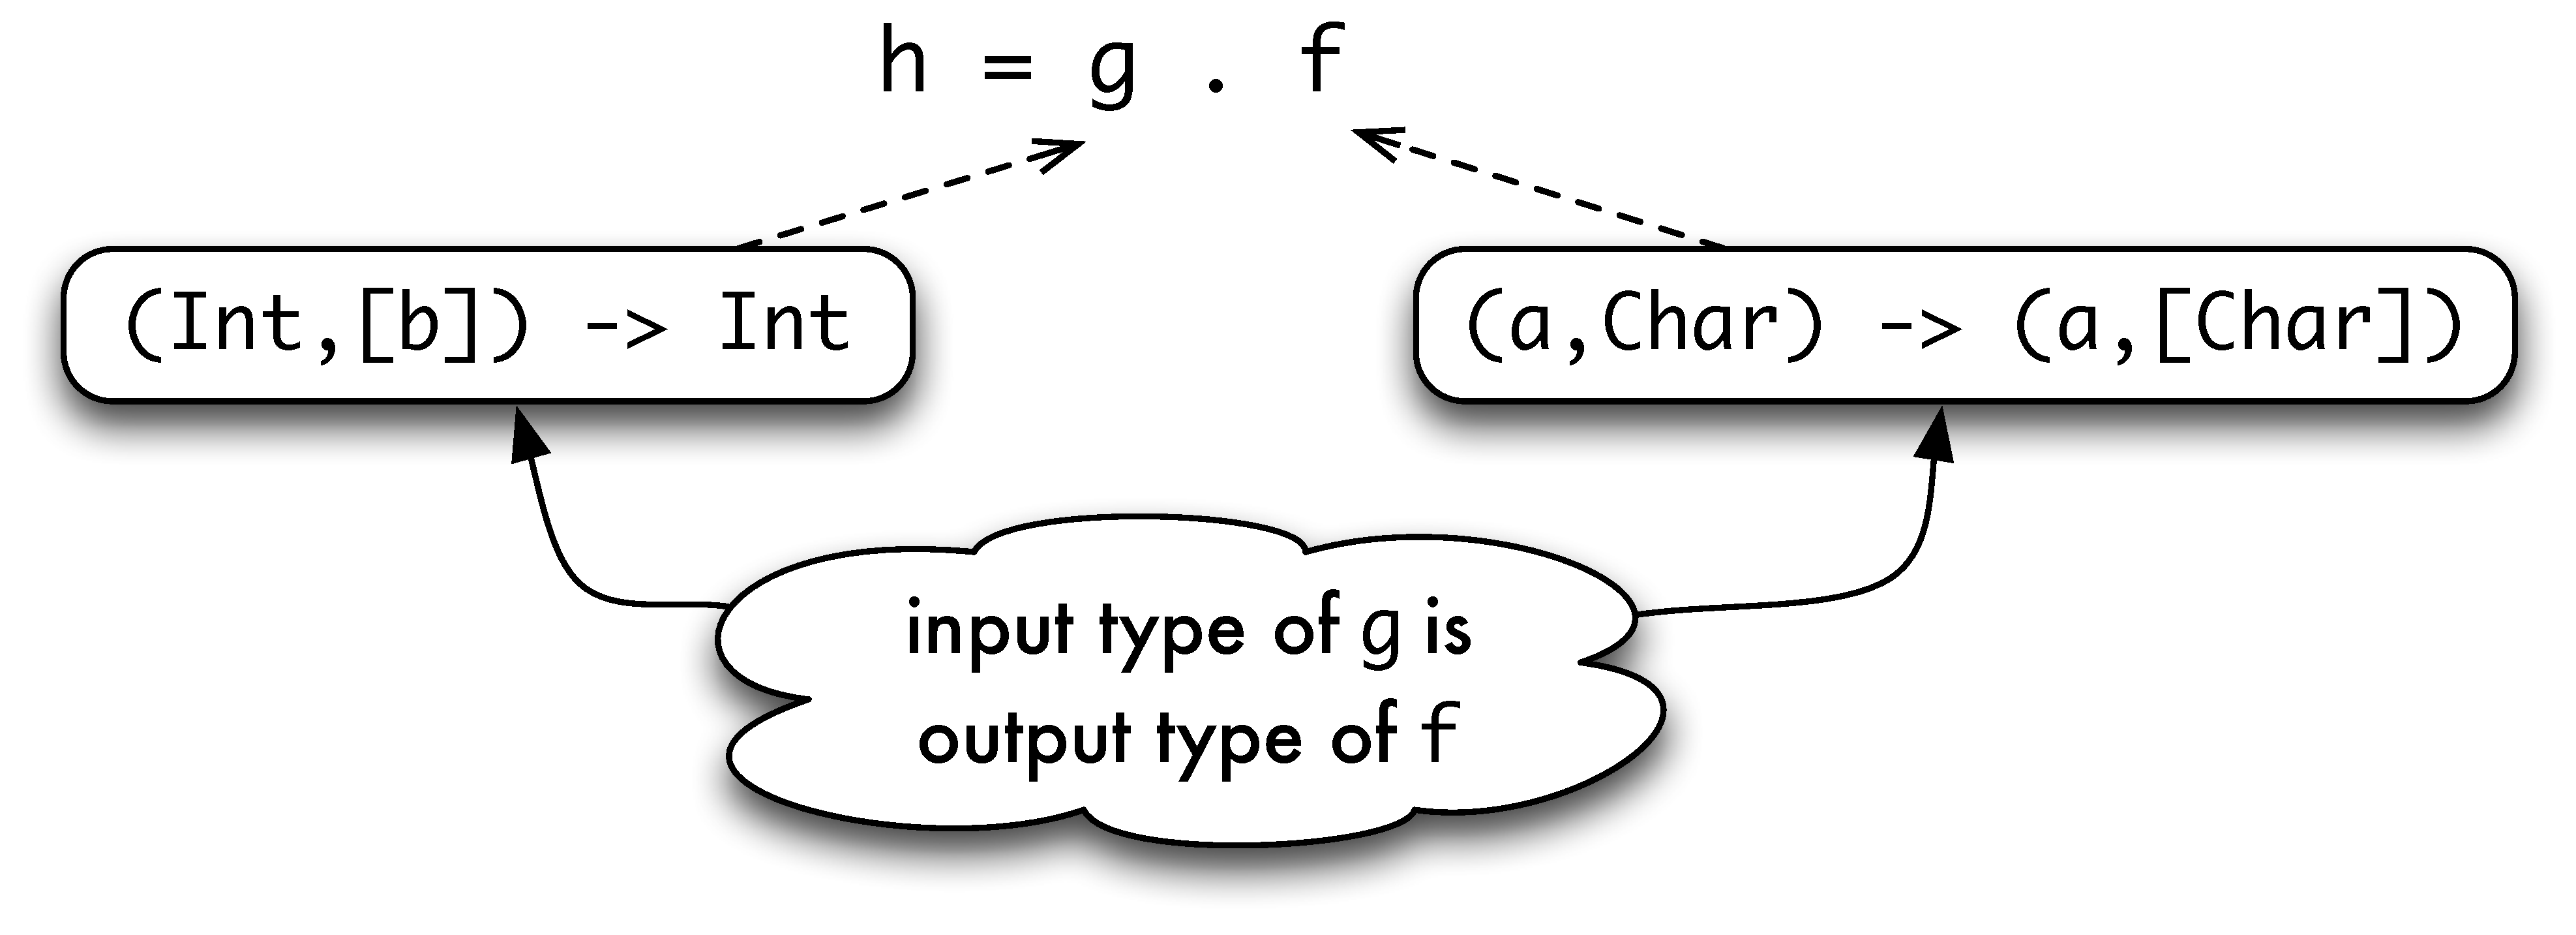
\includegraphics[width=4in]{Pictures/TypeCheckEx3.pdf}
\end{center}
Here we should recall the meaning of types which involve type variables;
we can see them as shorthand for sets of types. The output of \texttt{f}
is described by \texttt{(a,[Char])}, and the input of \texttt{g} by
\texttt{(Int,[b])}. We therefore have to look for types which meet
both these descriptions. We will now look at this general topic,
returning to the example in the course of this dicussion.



\subsection*{Unification}
\index{unification|(}

How are we to describe the types which meet the two descriptions
\texttt{(a,[Char])} and \texttt{(Int,[b])}?
\begin{center}
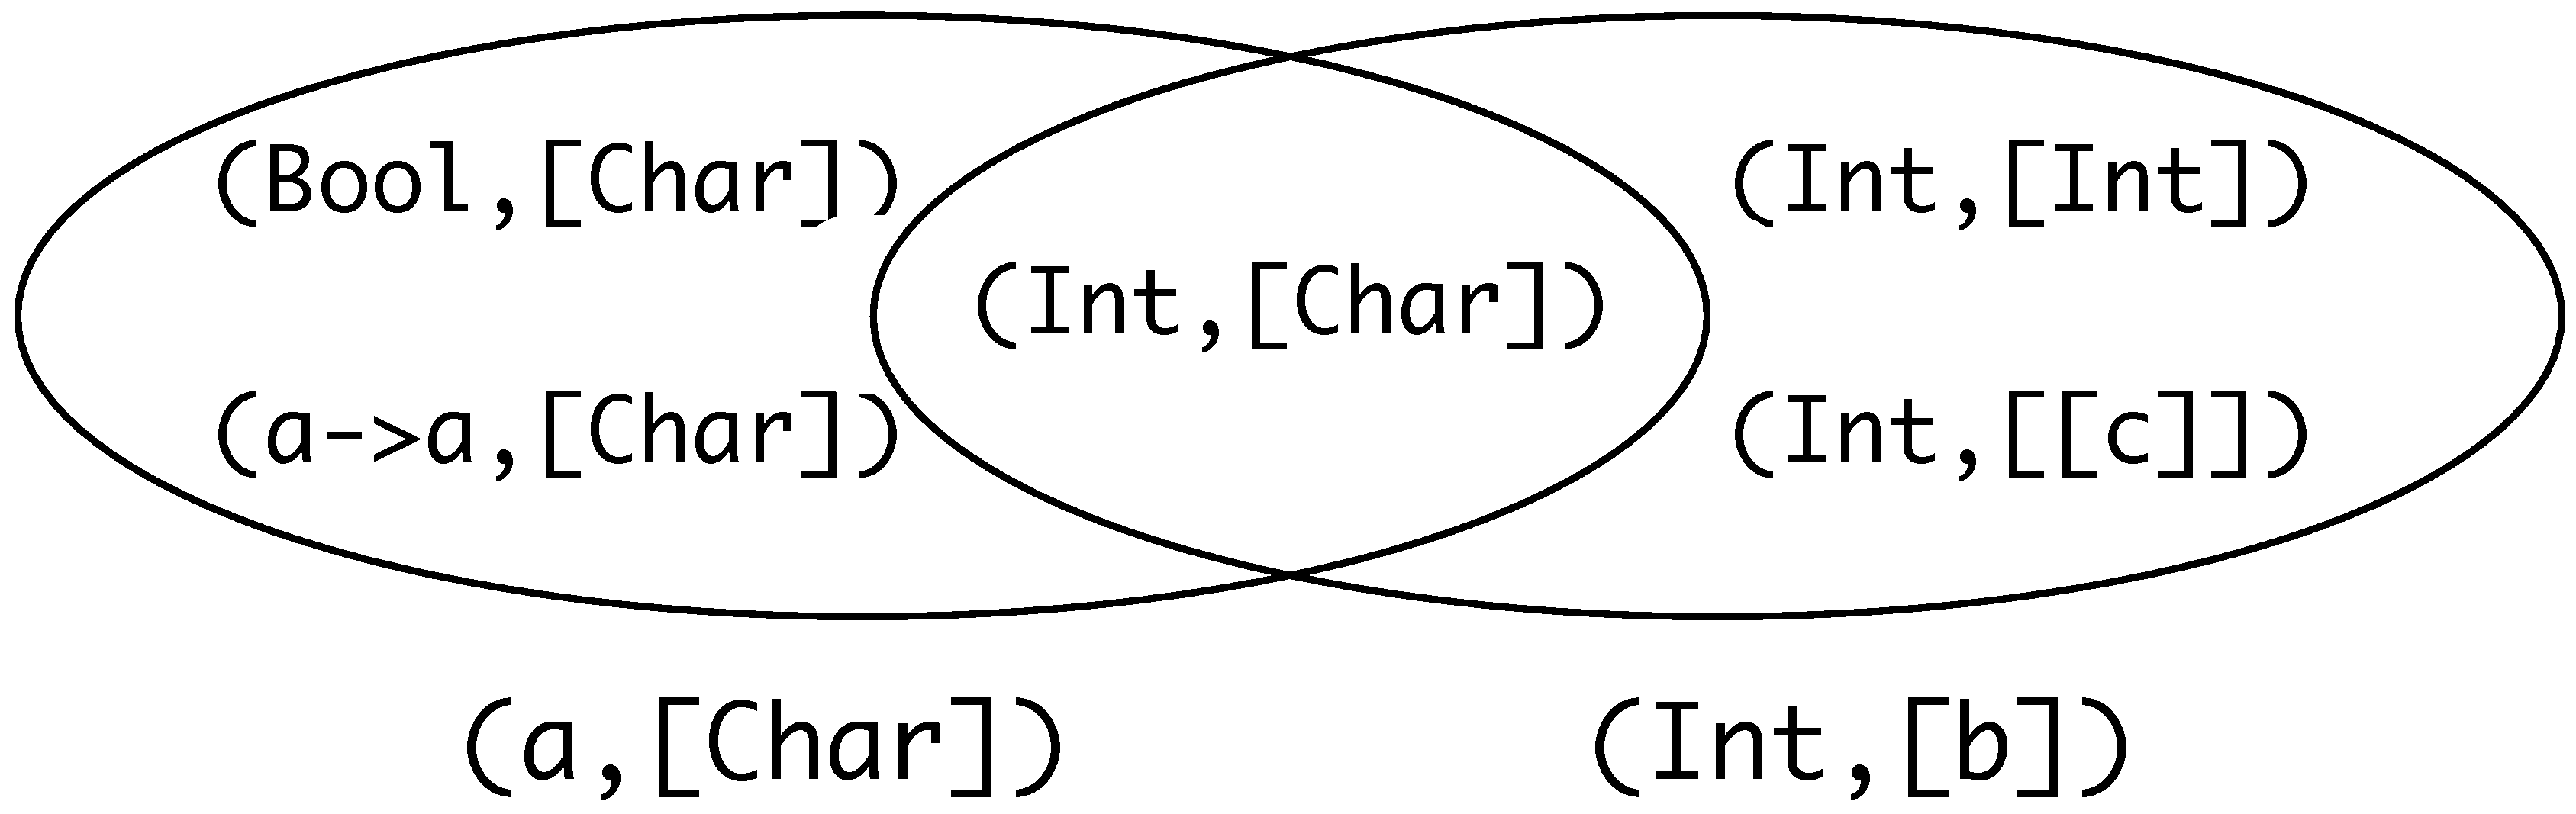
\includegraphics[width=3in]{Pictures/Unification.pdf}
\end{center}
As sets of types, we look for the intersection of the sets
given by \texttt{(a,[Char])} and \texttt{(Int,[b])}. How can we work
out a description of this intersection? Before we do this, we revise and
introduce some terminology. 

Recall that an \textbf{instance} of a
type is given by replacing a type variable or variables by type
expressions. A type expression is a common instance of two type
expressions if it is an instance of each expression. The most general
common instance of two expressions is a common instance \texttt{mgci}
with the property that every other common instance is an instance of
\texttt{mgci}.

Now we can describe the intersection of the sets given by two type expressions.
It is called the 
\textbf{unification} of the two, which is the \textbf{most general common
instance} of the two type expressions.

\subsubsection*{Example 3 (continued)}
In this example, we have
\begin{center}
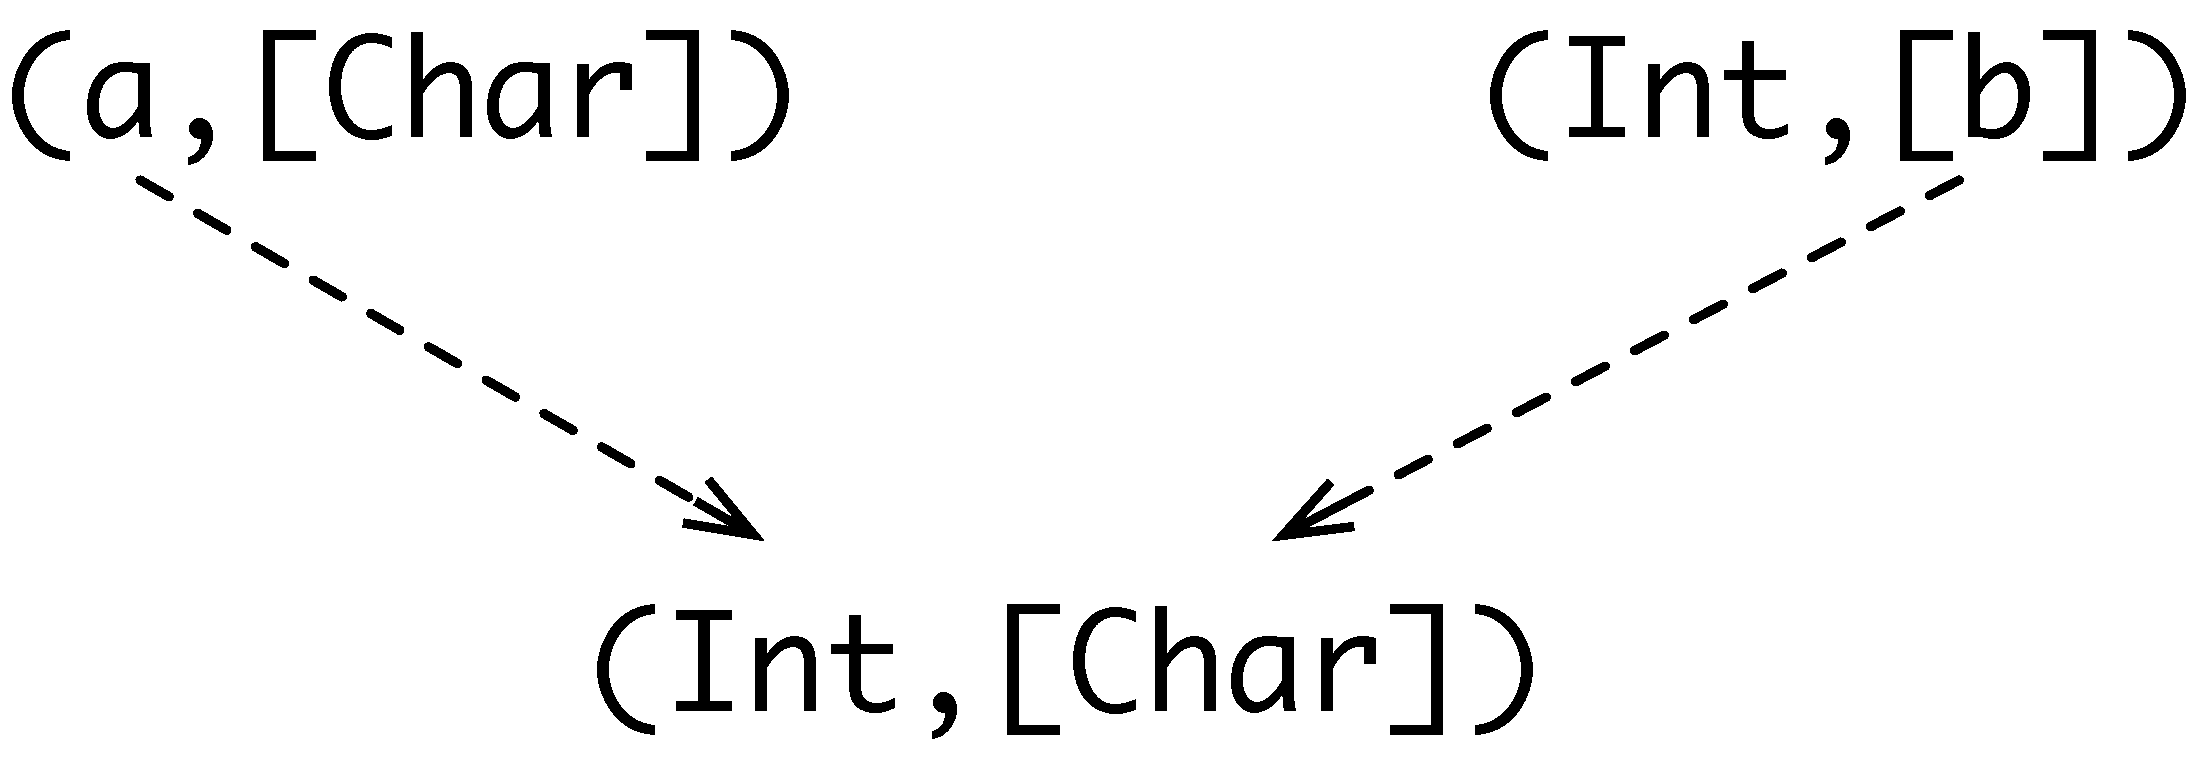
\includegraphics[width=2.5in]{Pictures/Unification2.pdf}
\end{center}
with a single type resulting. This means that the type \texttt{a} has to be \texttt{Int} and so the type of the function \texttt{h = g.f} is 
\begin{alltt}
h :: (Int,Char) -> Int
\end{alltt}
This concludes the discussion of example 3.
%\stoprule
\subsubsection*{Unification, revisited}


\noindent Unification need not result in a monotype. In the example of unifying
the types \texttt{(a,[a])} and \texttt{([b],c)},
\begin{center}
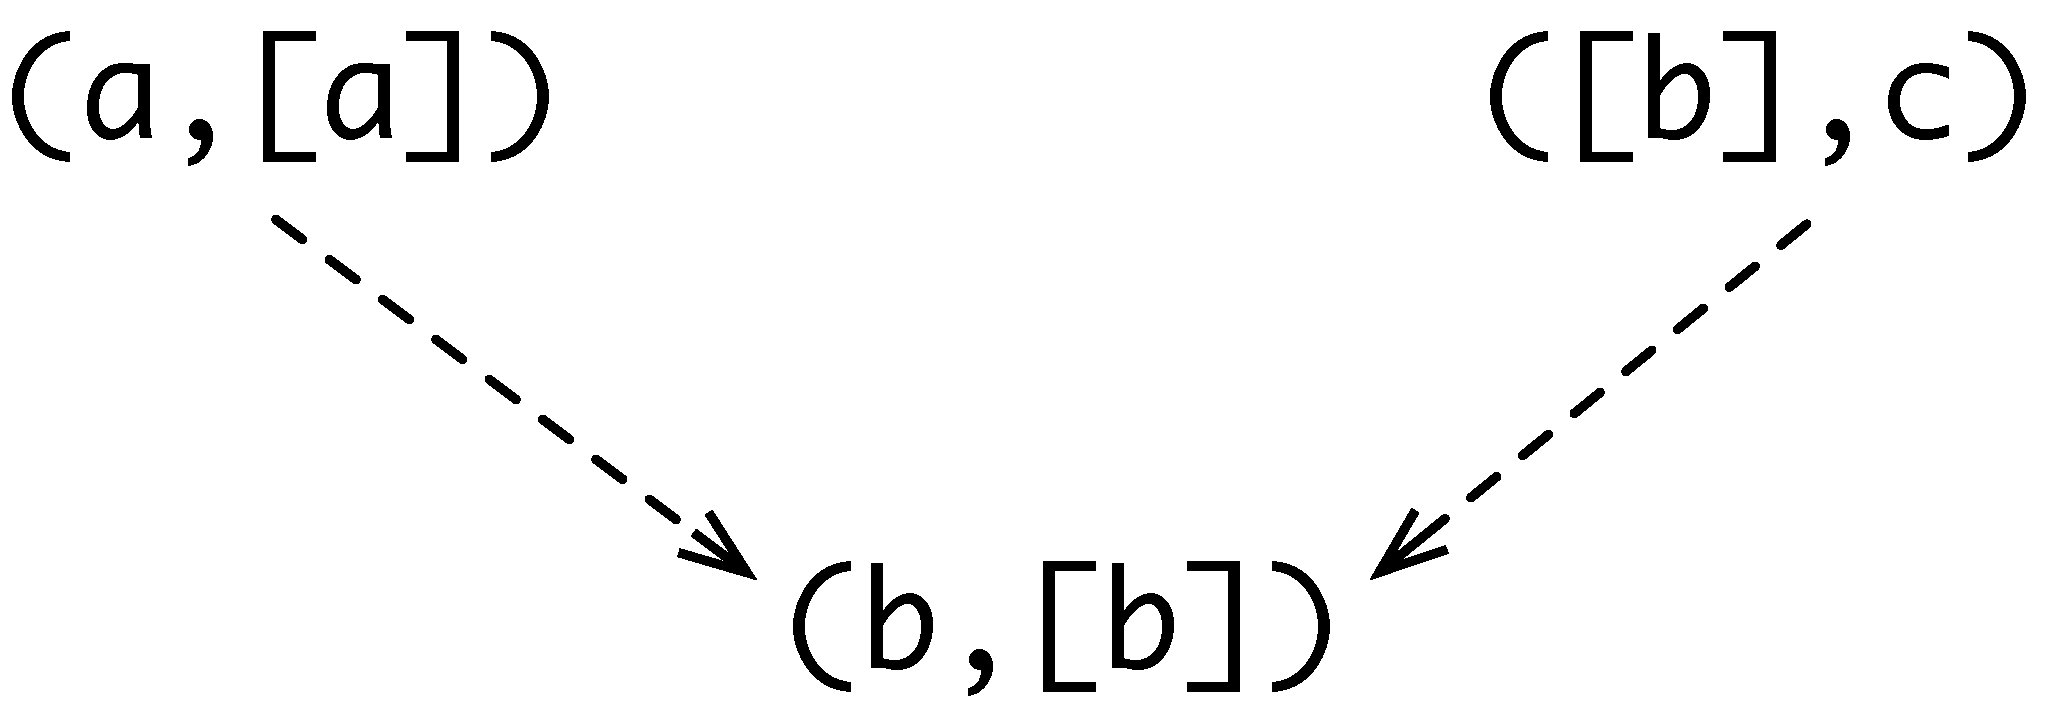
\includegraphics[width=2.5in]{Pictures/Unification3.pdf}
\end{center}
the result is the type \texttt{([b],[[b]])}. This is because the expression \texttt{(a,[a])}
constrains the type to have in its second component a list of elements of the first
component type, while the expression \texttt{([b],c)} constrains its first
component to be a list. Thus satisfying the two gives the type
\texttt{([b],[[b]])}. 

In the last example, note that there are many common instances of the
two type expressions, including \texttt{([Bool],[[Bool]])} and
\texttt{([[c]],[[[c]]])}, but neither of these examples is the unifier,
since \texttt{([b],[[b]])} is not an instance of either of them. On the
other hand, they are each instances of \texttt{([b],[[b]])}, as it is
the most general common instance, and so the unifier of the two type
expressions.

Not every pair of types can be unified: consider the case of 
\texttt{[Int] -> [Int]} and \hbox{\texttt{a -> [a]}}.
\begin{center}
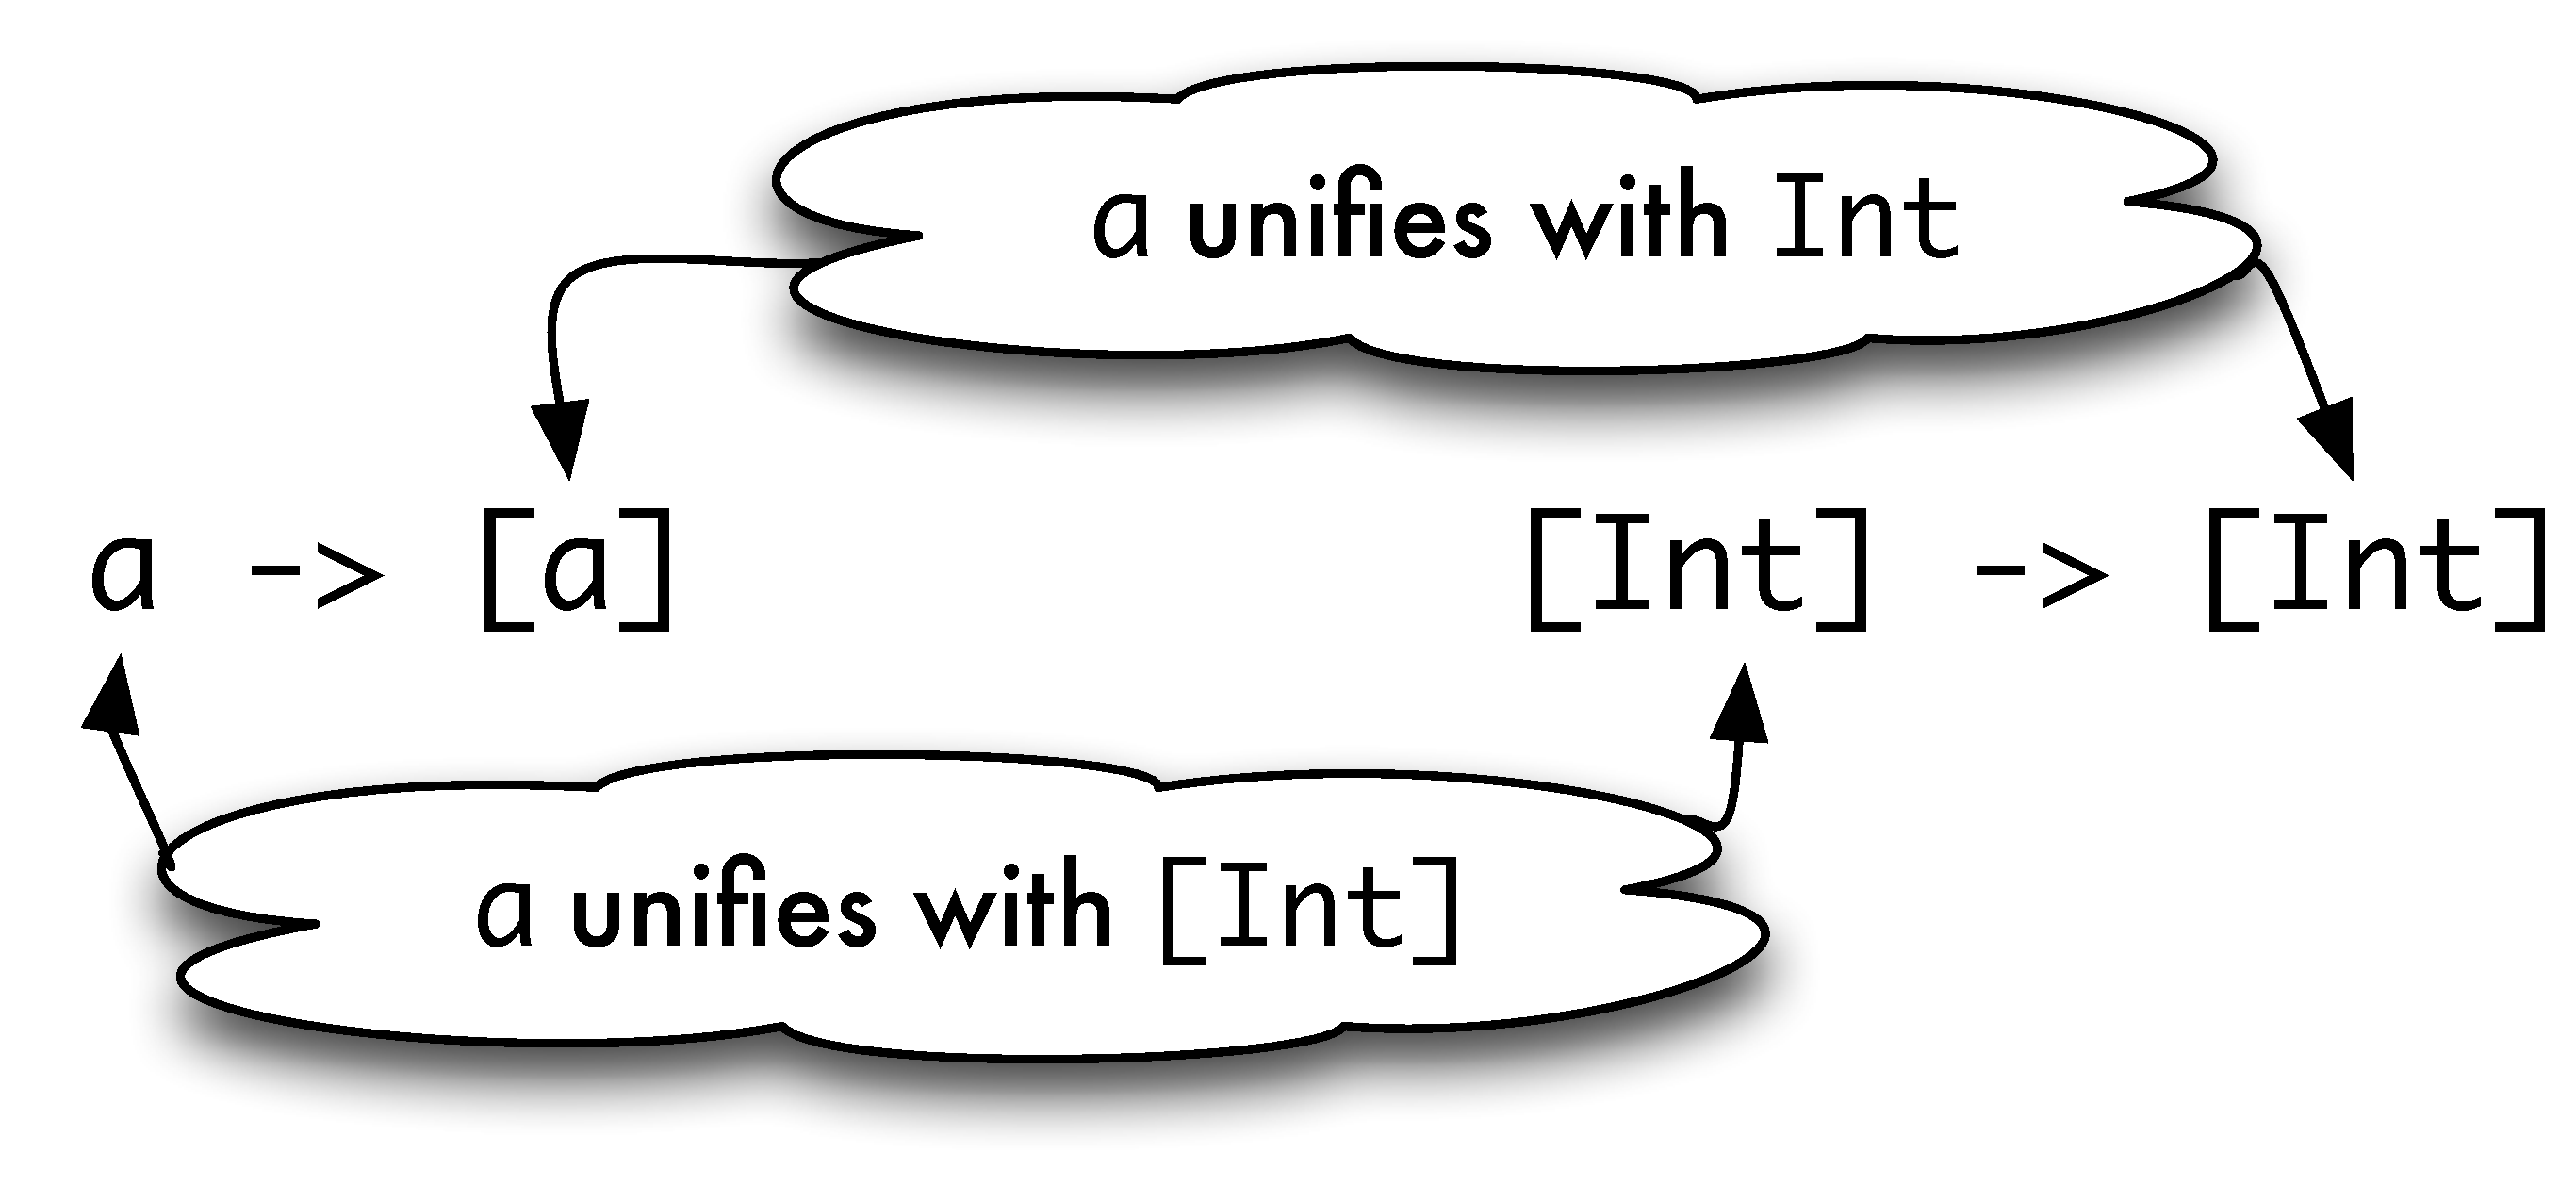
\includegraphics[width=3in]{Pictures/Unification4.pdf}
\end{center}
 Unifying the argument types requires
\texttt{a} to become \texttt{[Int]}, while unifying the result types
requires \texttt{a} to become \texttt{Int}; clearly these constraints
are inconsistent, and so the unification fails.
\index{unification|)}

\subsection*{Type-checking expressions}

As we saw in Section \ref{monoCheck}, function application is central to
expression formation. This means that type checking also hinges on
function applications. 

\subsubsection*{Type-checking polymorphic function application}
\index{type checking!polymorphic function application}
\begin{center}
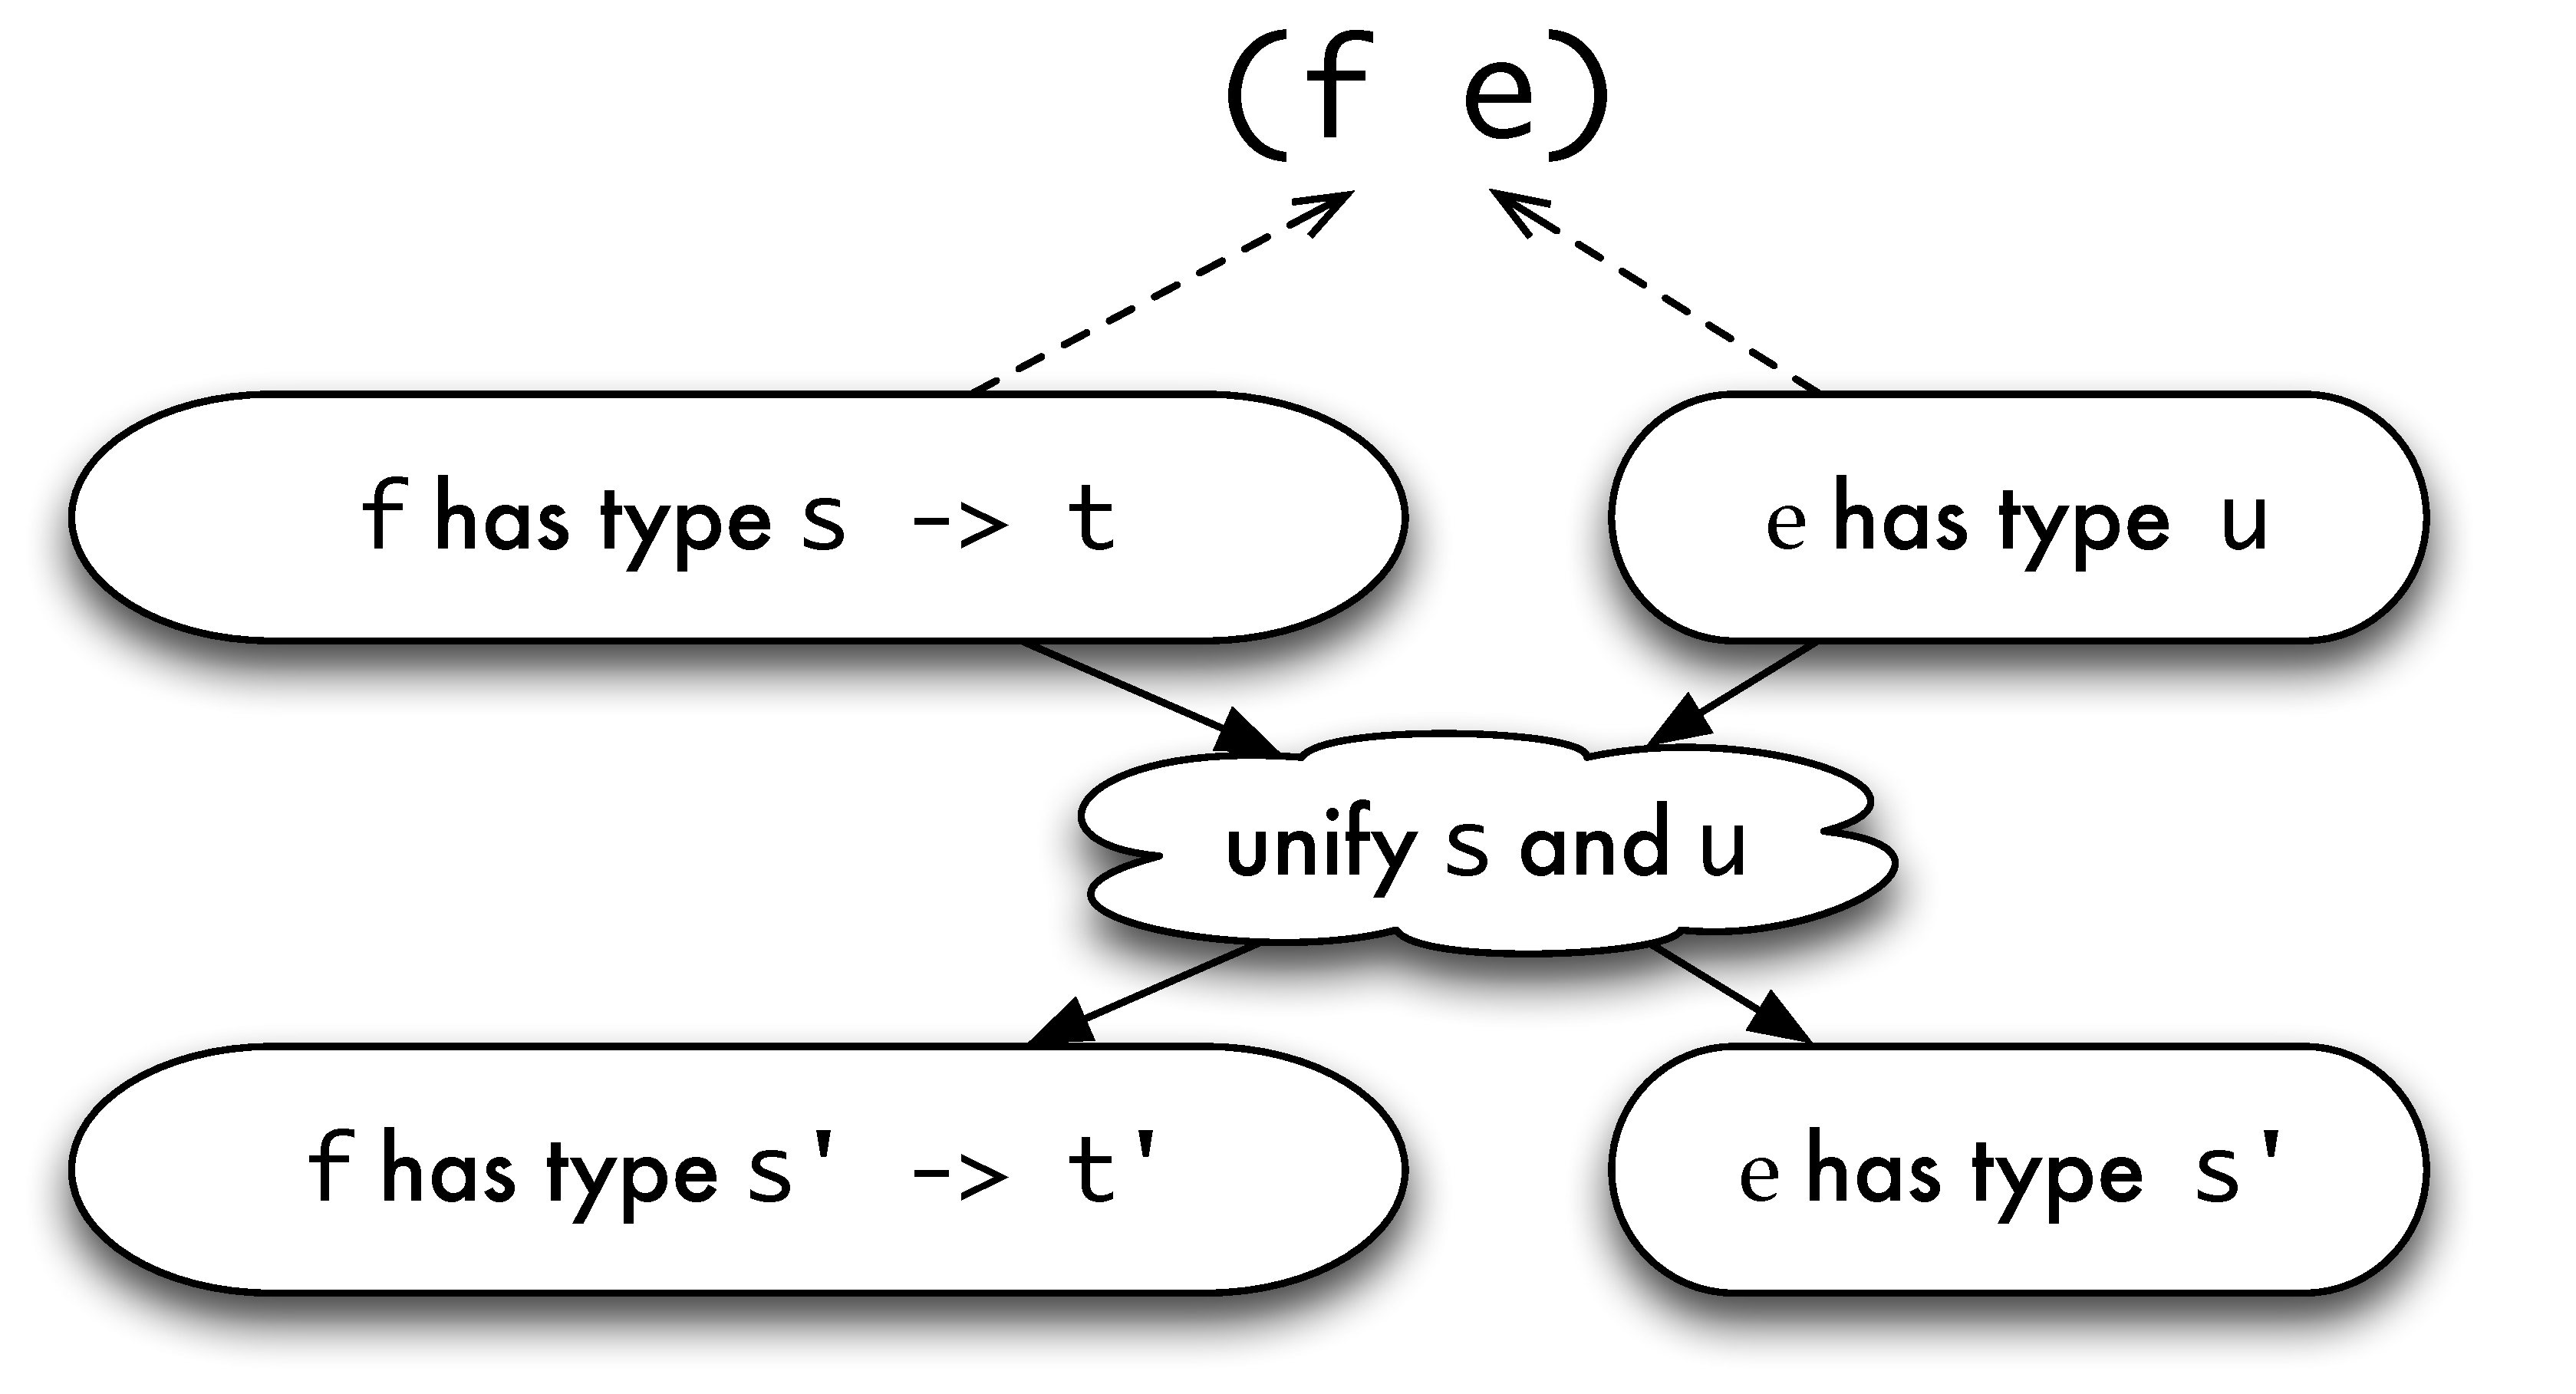
\includegraphics[width=3.5in]{Pictures/PolymorphicFunctionApp.pdf}
\end{center}
In applying a function \texttt{f ::\ s -> t} to
an argument \texttt{e ::\ u} we do not require that \texttt{s} and
\texttt{u} are equal, but instead that they are unifiable to a type \texttt{s'}, say, giving
\texttt{e ::\ s'} and \texttt{f ::\ s' -> t'}; the result in that case
is of type \texttt{t'.} 

\subsubsection*{Example 4}

As an example, consider the application
\texttt{map Circle} where \texttt{Circle} is one of the constructor functions for the \texttt{Shape} type.
\begin{alltt}
map :: (a -> b) -> [a] -> [b]
Circle :: Float -> Shape
\end{alltt}
Unifying \texttt{a -> b} and \texttt{Float -> Shape}
results in \texttt{a} becoming \texttt{Float} and \texttt{b} becoming
\texttt{Shape}; this gives
\begin{alltt}
map :: (Float -> Shape) -> [Float] -> [Shape]
\end{alltt}
and so
\begin{alltt}
map Circle :: [Float] -> [Shape]
\end{alltt}
As in the monomorphic case, we can use this discussion of typing and function application
in explaining type checking all aspects of
expressions. We now look at another example, before examining a more
technical aspect of type checking.

\subsubsection*{Example 5, \texttt{foldr} revisited}
\index{foldr@\texttt{foldr}!type of} 
In Section
\ref{foldPrimRec} we introduced the \texttt{foldr} function
\begin{alltt}
foldr f s []     = s\hfill(foldr.1)\index{foldr@\texttt{foldr}}
foldr f s (x:xs) = f x (foldr f s xs)\hfill(foldr.2)
\end{alltt}
which could be used to fold an operator into a list, as in
\begin{alltt}
foldr (+) 0 [2,3,1] = 2+(3+(1+0))
\end{alltt}
so that it appears as if \texttt{foldr} has the type given by
\begin{alltt}
foldr :: (a -> a -> a) -> a -> [a] -> a
\end{alltt}
In fact, the most general type of \texttt{foldr} is more general
than this. Suppose that the starting value has type \texttt{b}
and the elements of the list are of type \texttt{a}
\begin{alltt}
foldr :: (... -> ... -> ...) -> b -> [a] -> ...
\end{alltt}
Then we can picture the definition thus:
\begin{center}
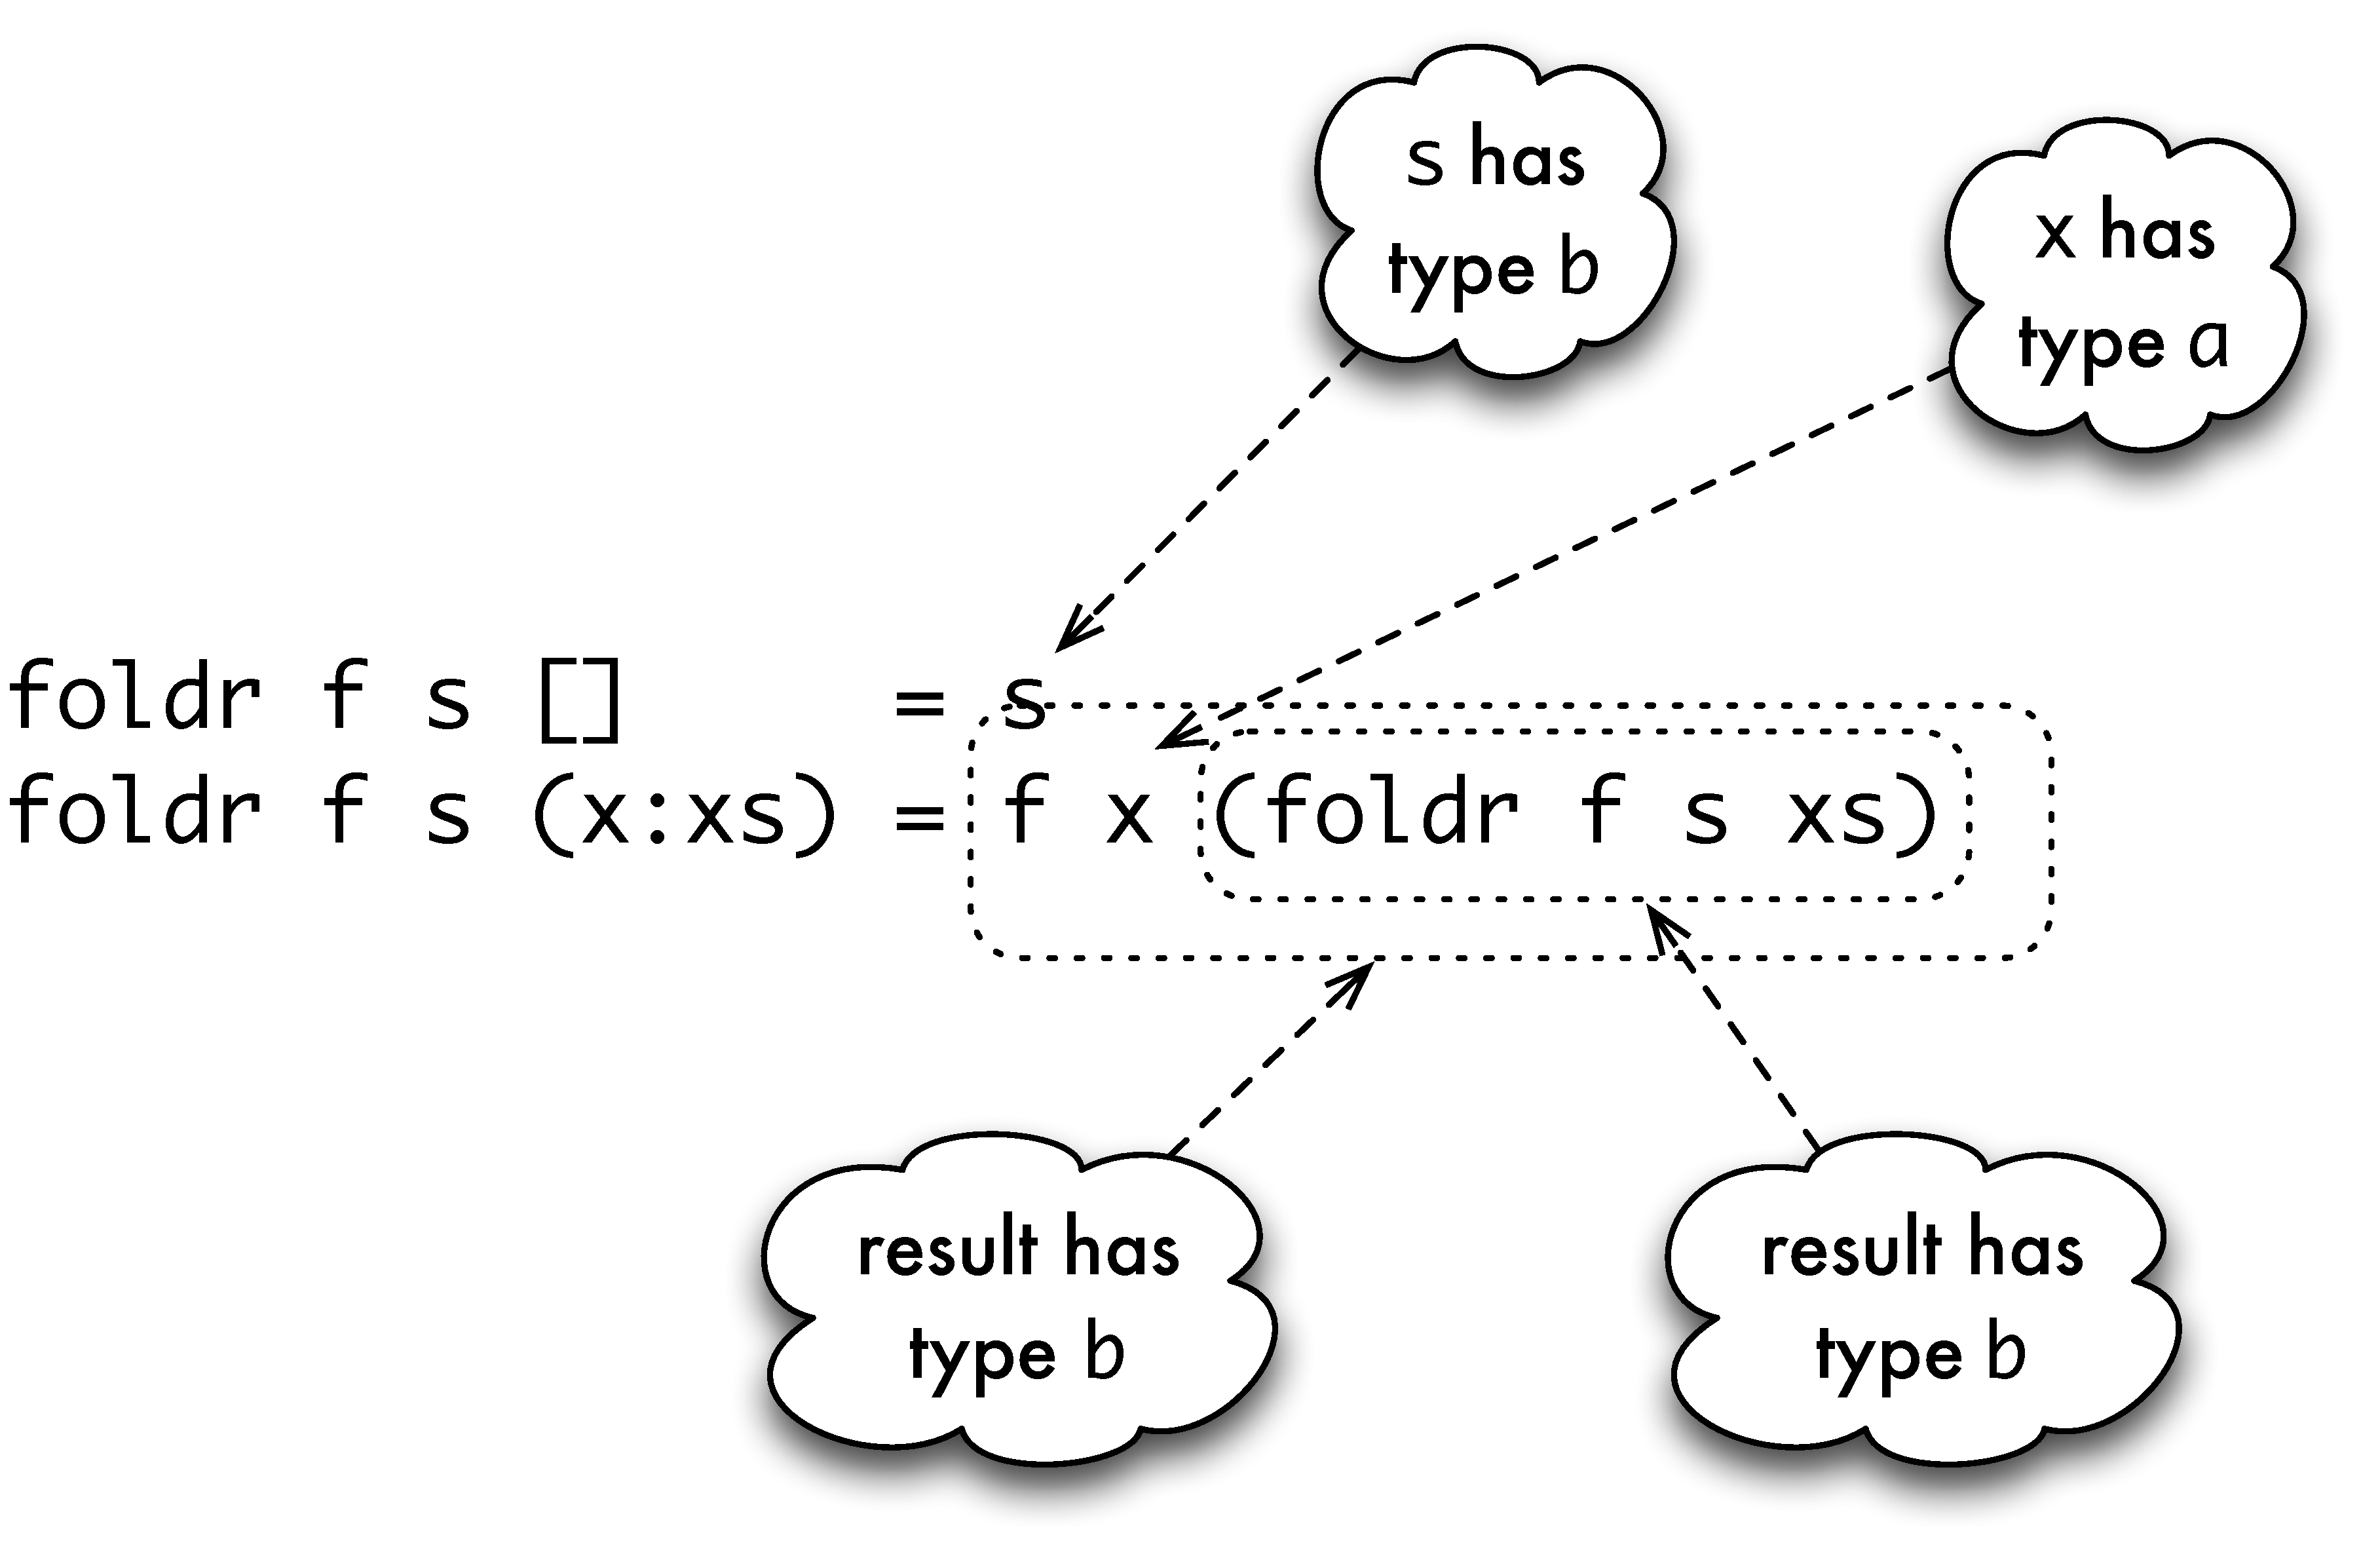
\includegraphics[width=4in]{Pictures/FoldrDef.pdf}
\end{center}
\texttt{s} is the result of the first equation, and so the result type of the
\texttt{foldr} function itself will be \texttt{b}, the type of \texttt{s}
\begin{alltt}
foldr :: (... -> ... -> ...) -> b -> [a] -> b
\end{alltt}
In the second equation, \texttt{f} is applied to \texttt{x} as first
argument, giving
\begin{alltt}
foldr :: (a -> ... -> ...) -> b -> [a] -> b
\end{alltt}
The second argument of \texttt{f} is the result of a \texttt{foldr}, and
so of type \texttt{b},
\begin{alltt}
foldr :: (a -> b -> ...) -> b -> [a] -> b
\end{alltt}
Finally, the result of the second equation is an application of
\texttt{f}; this result must have the same result type as the
\texttt{foldr} itself, \texttt{b}.
\begin{alltt}
foldr :: (a -> b -> b) -> b -> [a] -> b
\end{alltt}
With this insight about the type of \texttt{foldr} we were able to see that 
\texttt{foldr} could be used to define another whole cohort of list
functions, such as an insertion sort,
\begin{alltt}\minx{iSort}
iSort :: Ord a => [a] -> [a]
iSort = foldr ins []
\end{alltt}
in which \texttt{ins} has the type \texttt{Ord a => a -> [a] -> [a]}.
\vspace{10pt}

\subsection*{Polymorphic definitions and variables}
\index{type checking!polymorphic definitions}

Here we examine a more technical aspect of how type checking works over
polymorphic definitions; it may be omitted on first reading.

Functions and constants can be used at different types in the same
expression. A simple instance is
\begin{alltt}
expr = length ([]++[True]) + length ([]++[2,3,4]) \hfill (expr)
\end{alltt}
The first occurrence of \texttt{[]} is at \texttt{[Bool]}, whilst the second is at
\texttt{[Integer]}. This is completely legitimate, and is one of the advantages of
a polymorphic definition.
Now suppose that we replace the \texttt{[]} by a variable, and define
\begin{alltt}
funny xs = length (xs++[True]) + length (xs++[2,3,4]) \hfill (funny)
\end{alltt}
The variable \texttt{xs} is forced to have type \texttt{[Bool]} {\em and\/} type
\texttt{[Integer]}; it is forced to be polymorphic, in other words. This is
not allowed in Haskell, as there is no way of expressing the type of 
\texttt{funny}. It might be thought that
\begin{alltt}
funny :: [a] -> Int
\end{alltt}
was a correct type, but this would mean that \texttt{funny} would have all
the instance types
\begin{alltt}
funny :: [Int] -> Int
funny :: [[Char]] -> Int
  ...
\end{alltt}
which it clearly does not. We conclude that constants and variables are
treated differently: constants may very well appear at different
incompatible types in the same expression, variables cannot. 

What is the significance of disallowing the definition \texttt{(funny)} but
allowing the definition \texttt{(expr)}? Taking \texttt{(expr)} first, we have a polymorphic
definition of the form
\texttt{[] ::\ [a]}
and an expression in which 
\texttt{[]} occurs twice; the first occurrence is at \texttt{[Bool]}, the second at 
\texttt{[Integer]}. To allow these independent uses to occur, we
type-check each use
of a polymorphic definition with different type variables, so
that a constraint on one use does not affect any of the others.

On the other hand, how is the definition of \texttt{(funny)} disallowed? When we
type check the use of a variable we will not treat each instance as
being of an independent type. Suppose we begin with no constraint on \texttt{xs},
so \texttt{xs::t}, say. The first occurrence of \texttt{xs} forces
\texttt{xs::[Bool]}, the second requires \texttt{xs::[Integer]}; these
two constraints cannot be satisfied simultaneously, and thus the
definition \texttt{(funny)} fails to type check.

The crucial point to remember from this example is that the
definition of a function can't force any of
its arguments to be polymorphic. 

\subsection*{Function definitions}
\index{type checking!function definitions}

In type checking a function definition like \texttt{(fdef)} on page \pageref{fdef} above we have
to obey rules similar to the monomorphic case.
\begin{itemize}
\item Each of the guards \smsubscr{g}{i} must be of type \texttt{Bool}.
\item The value \smsubscr{e}{i} returned in each clause must have a type \smsubscr{s}{i} 
which is at least as general as \texttt{t}; that is, \smsubscr{s}{i} must have
\texttt{t} as an instance.
\item The pattern \smsubscr{p}{j} must be \textbf{consistent} with type
of that argument, namely \smsubscr{t}{j}. 
\end{itemize}
We take up a final aspect of type checking -- the impact of type classes
-- in the next section.

\begin{exercises}

\item
Do the following pairs of types -- listed vertically -- unify? If so, give a most general
unifier for them; if not, explain why they fail to unify.
\begin{alltt}
(Int -> b)  \hspace*{2cm} (Int,a,a)
(a -> Bool) \hspace*{2cm} (a,a,[Bool])
\end{alltt}

\item
Show that we can unify \texttt{(a,[a])} with
\texttt{(b,c)} to give \texttt{(Bool,[Bool])}. 

\item
Can the function
\begin{alltt}
f :: (a,[a]) -> b
\end{alltt}
be applied to the arguments \texttt{(2,[3])}, \texttt{(2,[])} and \texttt{(2,[True])};
if so, what are the types of the results?
Explain your answers.

\item
Repeat the previous question for the function
\begin{alltt}
f :: (a,[a]) -> a
\end{alltt}
Explain your answers.

\item
Give the type of \texttt{f [] []} if \texttt{f} has type
\begin{alltt}
f :: [a] -> [b] -> a -> b
\end{alltt}
What is the type of the function \texttt{h} given by the definition
\begin{alltt}
h x = f x x ?
\end{alltt}

\item
How can you use the Haskell system to check whether two type expressions are
unifiable, and if so what is their unification? Hint: you can make dummy definitions
in Haskell in which the defined value, \texttt{zircon}
say, is equated with itself:
\begin{alltt}
zircon = zircon
\end{alltt}
Values defined like this can be declared to have any type you wish.

\item
{[Harder]} Recalling the definitions of \texttt{curry} and
\texttt{uncurry} from Section \ref{curry}, what are the types of
\begin{alltt}
curry id
uncurry id
curry (curry id)
uncurry (uncurry id)
uncurry curry
\end{alltt}
Explain why the following expressions do not type-check:
\begin{alltt}
curry uncurry
curry curry
\end{alltt} 

\item
{[Harder]} Give an {\em algorithm\/} which decides whether two
type expressions are unifiable. If they are, your algorithm
should return a most general unifying substitution; if not, it
should give some explanation of why the unification fails.
\index{type checking!polymorphic|)}
\index{constraint!in type checking|)}
\index{type checking!constraints|)}
\index{polymorphism!type checking|)}
\end{exercises}

\section{Type checking and classes}
\label{typeCheckClasses}
\index{type checking!and classes|(}
\index{classes!type checking|(}

Classes in Haskell restrict the use of some functions, such as \texttt{==}, to
types in the class over which they are defined, in this case \texttt{Eq}. These
restrictions are apparent in the \textbf{contexts}\index{context} which appear in some types.
For instance, if we define
\begin{alltt}
member []     y = False\minx{member}
member (x:xs) y = (x==y) || member xs y
\end{alltt}
its type will be
\begin{alltt}
Eq a => [a] -> a -> Bool\index{context}
\end{alltt} 
because \texttt{x} and \texttt{y} of type \texttt{a} are compared for
equality in the definition, thus forcing the type 
\texttt{a} to belong to
the equality class \texttt{Eq}.

This section explores the way in which type checking takes place when overloading
is involved; the material is presented informally, by means of an
example. 

Suppose we are to apply the function \texttt{member} to an expression \texttt{e},
whose type is 
\begin{alltt}
Ord b => [[b]]
\end{alltt}
Informally, \texttt{e} is a list of lists of objects, which belong to
a type which carries an
ordering. In the absence of the contexts we would unify the type
expressions, giving
\begin{alltt}
member :: [[b]] -> [b] -> Bool \hspace*{2cm} e :: [[b]]
\end{alltt}
and so giving the application \texttt{member e}
the type \texttt{[b] -> Bool}. We do the same here,
but we also apply the unification to the contexts, producing the context
\begin{alltt}
(Eq [b] , Ord b)\hfill(ctx.1)\minx{Eq}\minx{Ord}
\end{alltt}
Now, we check and simplify the context.
\index{context!simplifying}
\begin{titemize}
\item The requirements in a context can only apply to type variables, so we need to eliminate
requirements like \texttt{Eq [b]}. The only way these can be eliminated is to use
the \texttt{instance} declarations. In this case the built-in instance
declaration
\begin{alltt}
instance Eq a => Eq [a] where ....
\end{alltt}
allows us to replace the requirement \texttt{Eq [b]} with \texttt{Eq b} in \texttt{(ctx.1)},
giving the new context
\begin{alltt}
(Eq b , Ord b)\hfill(ctx.2)
\end{alltt}
We repeat this process until no more instances apply.
\itempar
If we fail to reduce all the requirements to ones involving a type
variable, the application fails, and an error message would be generated. This
happens if we apply \texttt{member} to \texttt{[id]}; 
\begin{alltt}
    No instance for (Eq (a -> a))
      arising from a use of `member' at <interactive>:1:0-10
    Possible fix: add an instance declaration for (Eq (a -> a))
    In the expression: member [id]
    In the definition of `it': it = member [id]
\end{alltt}
since \texttt{id} is a function, whose type is not it the class \texttt{Eq}.
\index{type checking!instance error}

\item We then simplify the context using the \texttt{class} definitions. In our
example we have both \texttt{Eq b} and \texttt{Ord b}, but recall that
\minx{class}
\begin{alltt}
class Eq a => Ord a where ...
\end{alltt}
so that any instance of \texttt{Ord} is automatically an instance of \texttt{Eq};
this means that we can simplify \texttt{(ctx.2)} to
\begin{alltt}
Ord b
\end{alltt}
This is repeated until no further simplifications result.
\end{titemize}
For our example, we thus have the type
\begin{alltt}
member e :: Ord b => [b] -> Bool
\end{alltt}
This three-stage
process of unification, checking (with instances) and simplification is
the general pattern for type checking with contexts in Haskell. 

Finally, we should explain how contexts are introduced into the types of the
language. They originate in types for the functions in class declarations, so
that, in the example of the \texttt{Info} class from earlier in the chapter, we have
\begin{alltt}
examples :: Info a => [a]\minx{Info}
size     :: Info a => a -> Int
\end{alltt}
The type checking of
functions which use these overloaded functions will propagate
and combine the contexts as we have seen above.

We have seen informally how the Haskell type system accommodates type
checking for the overloaded names which belong to type classes. A more
thorough overview of the technical aspects of this, including a
discussion of the `monomorphism restriction' which needs to be placed on
certain polymorphic bindings, is to be found in the Haskell 2010
report \cite{haskell2010}.

\index{type checking!and classes|)}
\index{classes!type checking|)}

\begin{exercises}

\item
Give the type of each of the individual conditional
equations which follow, and discuss the
type of the function which together they define.
\begin{alltt}
merge (x:xs) (y:ys) 
  | x<y         = x : merge xs (y:ys)
  | x==y        = x : merge xs ys
  | otherwise   = y : merge (x:xs) ys
merge (x:xs) []    = (x:xs)
merge []    (y:ys) = (y:ys)
merge []    []     = []
\end{alltt}

\item
Define a polymorphic sorting function, and show how its type is derived from
the type of the ordering relation
\begin{alltt}
compare :: Ord a => a -> a -> Ordering
\end{alltt}

\item
Investigate the types of the following numerical functions; you will
find that the types refer to some of the built-in numeric classes.
\begin{alltt}
mult x y = x*y
divide x = x `div` 2
share x  = x / 2.0
\end{alltt}
Recall that these can be given more restrictive types, such as
\begin{alltt}
divide :: Int -> Int
\end{alltt}
by explicitly asserting their types as above.
\end{exercises}

\index{type checking|)}














\begin{summary}
This chapter has shown how names such as \texttt{read} and \texttt{show} and
operators like \texttt{+} can be overloaded to have different definitions at
different types. The mechanism which enables this is the system of Haskell
classes. A \texttt{class} definition contains a signature which contains
the names and types of operations which must be supplied if a type is to
be a member of the class. For a particular type, the function definitions are
contained in an \texttt{instance} declaration.

In giving the type of a function, or introducing a class or an instance, we can
supply a context, which constrains the type variables occurring. Examples
include
\begin{alltt}
member :: Eq a => [a] -> a -> Bool\minx{Eq}
instance  Eq a => Eq [a] where ....
class     Eq a => Ord a  where ....\minx{Ord}
\end{alltt}
In the examples, it can be seen that \texttt{member} can only be used over types
in the class \texttt{Eq}. Lists of \texttt{a} can be given an equality, provided
that \texttt{a} itself can; types in the class \texttt{Ord} must already be in the
class \texttt{Eq}. 
After giving examples of the various mechanisms, we looked at the classes in
the standard preludes of Haskell. 

We concluded the chapter with a discussion of how type checking of expressions and definitions is performed in
Haskell, initially in the monomorphic case, and then in full generality with polymorphic and overloaded functions. In that case we saw type checking as
a process of extracting and consolidating constraints which come from the 
unification of type expressions which contain type variables. 
\end{summary}


%\end{document}

%\documentclass{book}\usepackage{sjtfonts}\usepackage{includegraphics}\usepackage{alltt}\usepackage{latexsym}
%\usepackage{array}
%\begin{document}\input{defs0}%		miradefs.tex 		    June 1994

% opening and closing a quoted Miranda section

\newcommand{\mira}{\noindent\hrulefill\nopagebreak\so}
\newcommand{\arim}{\nopagebreak\st\hrulefill\\}

% backslash in the Miranda environment
% Only feasible approach is to use \verb+\+
% in line!

%\newcommand{\bs}{$\mi\backslash\!\!$}
%\newcommand{\lbs}{\mbox{\verb+\+}}

% ignoring part of the input

\newcommand{\ignore}[1]{}

% a blank line in a Miranda section

\newcommand{\bl}{\mbox{\ }}

% Signalling a diffculty.

\definecolor{light-gray}{gray}{0.95}

\newcommand{\beware}[2]
 {\medskip\noindent\colorbox{light-gray}{\parbox{\textwidth}
 {\mbox{\large\textbf{#1}} \medskip\noindent\\ #2}\medskip\noindent}}

% Subscripting in Miranda text
\newcommand{\subscr}[2]{\mbox{${\mbox{\texttt{#1}}}_{\mbox{\texttt{#2}}}$}}

%\newcommand{\subscr}[2]{\mbox{${\mbox{\mi #1}}_{\mbox{\smtt #2}}$}}
\newcommand{\aone}{\subscr{a}{1}}
\newcommand{\atwo}{\subscr{a}{2}}
\newcommand{\ak}{\subscr{a}{k}}

\newcommand{\aoneone}{\subscr{a}{1,1}}

\newcommand{\eone}{\subscr{e}{1}}
\newcommand{\etwo}{\subscr{e}{2}}
\newcommand{\ei}{\subscr{e}{i}}
\newcommand{\er}{\subscr{e}{r}}

\newcommand{\fone}{\subscr{f}{1}}
\newcommand{\fl}{\subscr{f}{l}}

\newcommand{\gone}{\subscr{g}{1}}
\newcommand{\gtwo}{\subscr{g}{2}}
\newcommand{\gi}{\subscr{g}{i}}
\newcommand{\gr}{\subscr{g}{r}}

\newcommand{\hone}{\subscr{h}{1}}
\newcommand{\hl}{\subscr{h}{l}}

\newcommand{\pone}{\subscr{p}{1}}
\newcommand{\ptwo}{\subscr{p}{2}}
\newcommand{\pk}{\subscr{p}{k}}

\newcommand{\qone}{\subscr{q}{1}}
\newcommand{\qtwo}{\subscr{q}{2}}
\newcommand{\qk}{\subscr{q}{k}}

\newcommand{\rone}{\subscr{r}{1}}
\newcommand{\rtwo}{\subscr{r}{2}}

\newcommand{\tone}{\subscr{t}{1}}
\newcommand{\ttwo}{\subscr{t}{2}}
\newcommand{\tn}{\subscr{t}{n}}

\newcommand{\vone}{\subscr{v}{1}}
\newcommand{\vtwo}{\subscr{v}{2}}
\newcommand{\vn}{\subscr{v}{n}}

% for regular expressions

\newcommand{\stone}{\subscr{st}{1}}
\newcommand{\sttwo}{\subscr{st}{2}}
\newcommand{\stn}{\subscr{st}{n}}
\newcommand{\rthree}{\subscr{r}{3}}

\newcommand{\eps}{$\varepsilon$}
\newcommand{\trans}[1]{\stackrel{\mbox{\tt #1}}{\longrightarrow}}



% superscript in Miranda text

\newcommand{\superscr}[2]{\mbox{${\mbox{\mi #1}}^{\mbox{\smtt #2}}$}}

% Not equals in Miranda text

\newcommand{\noteq}{\makebox[0pt][l]{=}/}
\newcommand{\overslash}{\makebox[0pt][l]{/}}

% Definitions in complexity chapter

\newfont{\oldSym}{cmsy10}
\newcommand{\Th}{\boldmath$\oldSym\Theta$}
\newcommand{\pow}[1]{\^{}#1}
\newcommand{\leqq}{$\leq$}
\newcommand{\geqq}{$\geq$}
\newcommand{\lll}{$\ll$}
\newcommand{\eqq}{$\equiv$}
\newcommand{\ltwo}{\subscr{log}{2}}

% Indexing

\newcommand{\minx}[1]{\index{#1@{\ttfamily{}#1}}}
\setcounter{chapter}{13}\setcounter{page}{231}

\chapter{Algebraic types}
\chapstart
\label{algTypes}
\index{algebraic type|(}

\begin{figure}[t]
\begin{center}
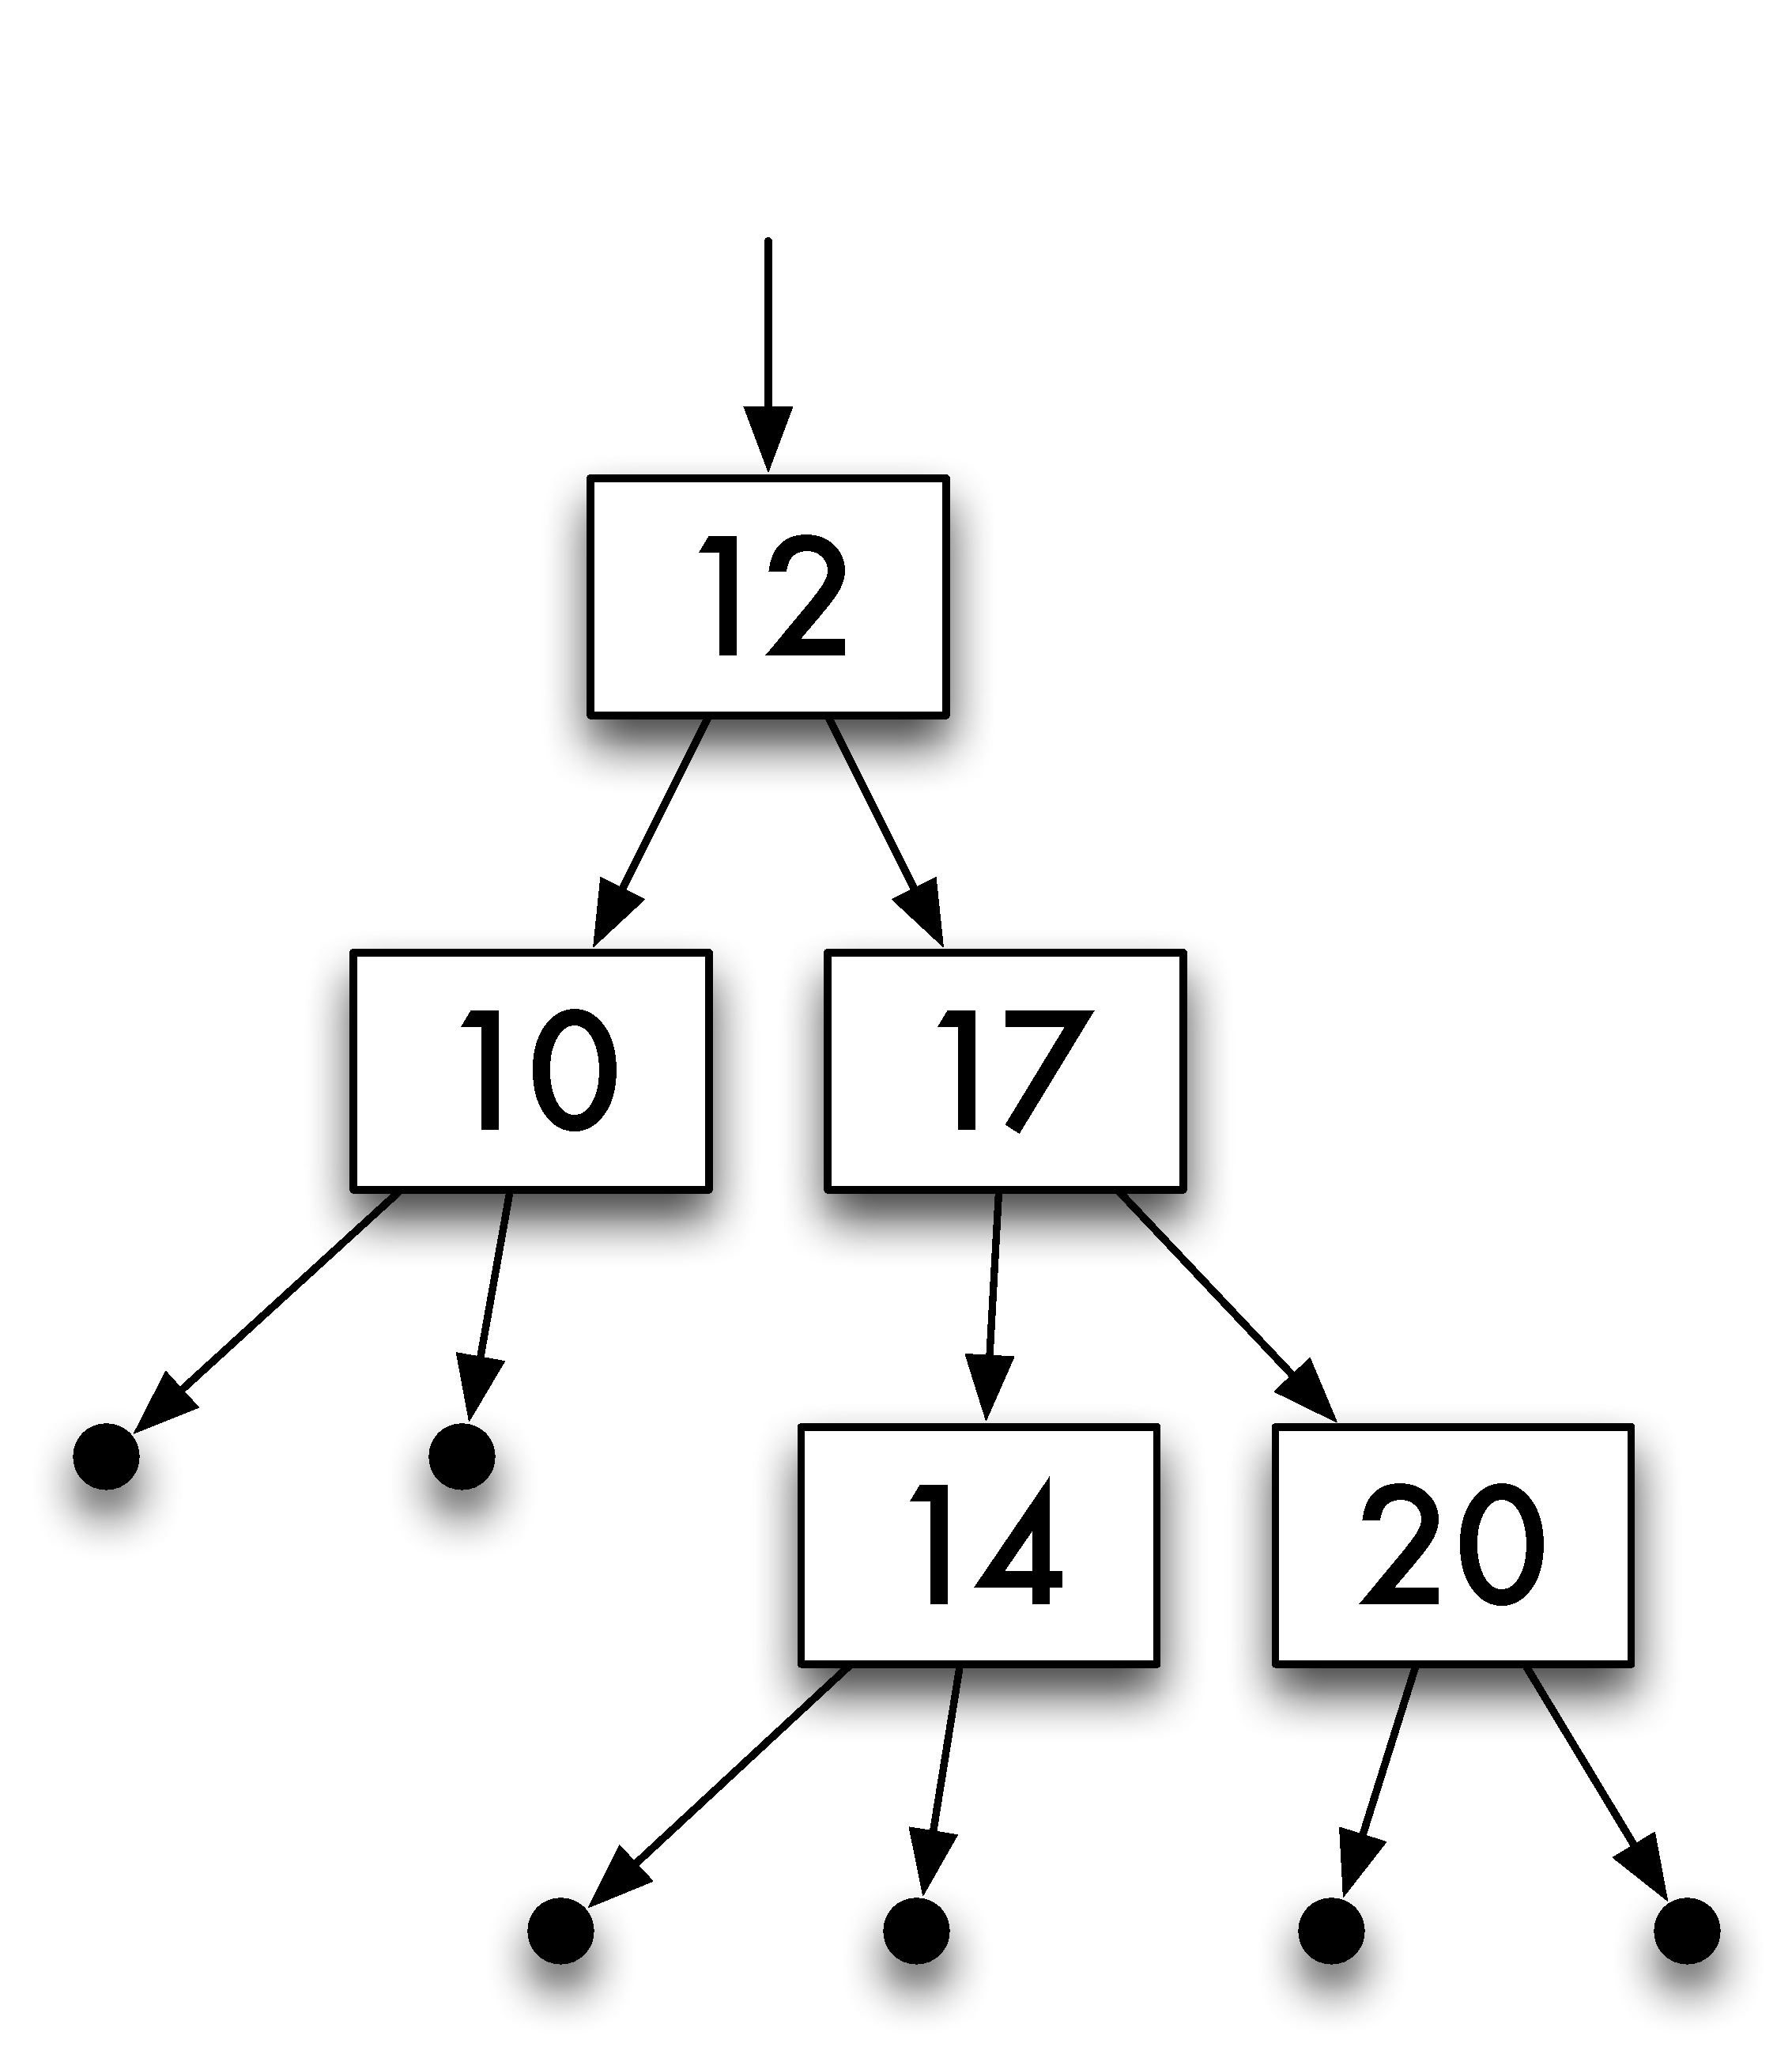
\includegraphics[width=3in]{Pictures/NewTree.pdf}
\end{center}
\caption{An example of a tree of integers.}
\label{treeFig}
\end{figure}

So far in our discussion of Haskell we have been able to model entities using
\begin{titemize}
\item the base types, \texttt{Int}, \texttt{Float}, \texttt{Bool} and \texttt{Char}, and
\item composite types: tuple types, \texttt{(\tone,\ttwo,\ldots,\subscr{t}{n})};
list types,
\texttt{[\tone]}; and function types, \texttt{(\tone\ -> \ttwo)}; where 
\texttt{\tone}, \ldots, \texttt{\subscr{t}{n}} are themselves types,
\item algebraic types, including enumerated types, as introduced in Section \ref{EnumTypes}, and product and sum type, first given in Section \ref{introAlg}.
\end{titemize}
This gives a wide range of types to use in modelling different domains in Haskell. This chapter completes our coverage of the topic of algebraic types and looks at two extensions in some detail:

\begin{titemize}
\item The types can be \textbf{recursive}\index{algebraic type!recursive|see{recursive type}};
we can use the type we are defining,
\texttt{Typename}, as (part of) any of the component types, as in the definition of numeric trees ``\texttt{NTree}s'':
\begin{alltt}
data NTree = NilT |\minx{NTree}
             Node Integer NTree NTree
\end{alltt}
an illustration of a tree from \texttt{NTree} is given in Figure \ref{treeFig}. Recursion in \texttt{data} type definitions gives us
lists, trees and many other useful data structures.
\item The name of the type being defined can be followed by one or more type
variables which may be used on the right-hand side, making the definition
\textbf{polymorphic}.\index{algebraic type!polymorphic} An example built-into Haskell is the \texttt{Maybe} type,
\begin{alltt}
data Maybe a = Nothing | Just a
\end{alltt}
which can be used in modelling program errors.
\end{titemize}
Recursive polymorphic types combine these two ideas, and this powerful
mixture provides types which can be reused in many different situations --
the built-in type of lists is an example which we have already seen. We'll look again at the \texttt{NTree} and \texttt{Maybe} types later in this chapter, and other
examples are given in the sections which follow.

\section{Algebraic type definitions revisited}
\label{algRevisited}
Algebraic data type definitions are introduced by the keyword \texttt{data}, followed by
\index{data@\texttt{data} type|see{algebraic type}}
the name of the type, an equals sign and then the
\textbf{constructors} of the\index{constructor}
type being defined.  The name of the type and the names of
constructors begin with
capital letters.

The general form of the algebraic type definitions which we have seen so far is \index{algebraic type!general form of definition}
\begin{alltt}
data Typename \hfill (Typename)
  = \subscr{Con}{1} \subscr{t}{11} \ldots \subscr{t}{1\subscr{k}{1}} | 
    \subscr{Con}{2} \subscr{t}{21} \ldots \subscr{t}{2\subscr{k}{2}} | 
        ....
    \subscr{Con}{n} \subscr{t}{n1} \ldots \subscr{t}{n\subscr{k}{n}}   
\end{alltt}
Each \texttt{\subscr{Con}{i}} is a constructor, followed by 
\subscr{k}{i}\ types, where \subscr{k}{i}\ is a non-negative integer which may
be zero. We build elements of the type \texttt{Typename} by applying these constructor
functions to arguments of the types given in the definition, so that
\begin{alltt}
\subscr{Con}{i} \subscr{v}{i1} \ldots \subscr{v}{i\subscr{k}{i}}
\end{alltt}
will be a member of the type \texttt{Typename} if \subscr{v}{ij} is 
in \subscr{t}{ij} for \texttt{j} ranging from \texttt{1} to \subscr{k}{i}. 
Reading the constructors as functions, the 
definition \texttt{(Typename)} gives the constructors the following
types
\begin{alltt}
\subscr{Con}{i} :: \subscr{t}{i1} -> \ldots -> \subscr{t}{i\subscr{k}{i}} -> Typename
\end{alltt}
Of the examples we have seen so far, enumerated types have constructors which take no arguments, 
\begin{alltt}
data Season = Spring | Summer | Autumn | Winter\minx{Season}
\end{alltt}
product types have a single constructor, 
\begin{alltt}
data People = Person Name Age \minx{People}
\end{alltt}
and sum types are the most general: they have a number of constructors taking different arguments, as in the definition
\begin{alltt}\minx{Shape}
data Shape = Circle Float |
             Rectangle Float Float
\end{alltt}
Definitions over algebraic types use pattern matching both to distinguish between different alternatives and to extract components from particular elements:
\begin{alltt}
area :: Shape -> Float
area (Circle r)      = pi*r*r
area (Rectangle h w) = h*w
\end{alltt}
As we discussed in Section \ref{haskellClasses},  Haskell has a number of built-in classes including
 \texttt{Eq},  \texttt{Ord}, 
  \texttt{Enum}, \texttt{Show}, and \texttt{Read}. When we introduce a new algebraic type it's possible to \texttt{derive} instances of these classes for the new type, like this:
\begin{alltt}\minx{Season}
data Season = Spring | Summer | Autumn | Winter 
              deriving (Eq,Ord,Enum,Show,Read)
\end{alltt}
We can thus compare seasons for equality and order, write expressions of
the form \texttt{[Spring .. Autumn]} denoting the list \texttt{[Spring, Summer, Autumn]}, and \texttt{show} and read values of the type.


\begin{exercises}





\item
Reimplement the library database\index{library database}
of Section \ref{library} to use an
algebraic type like \texttt{People} rather than a pair. Compare
the two approaches to this example.

\item
The library database of Section \ref{library} is to be extended in the
following ways.
\begin{titemize}
\item CDs and videos as well as books are available for loan.
\item A record is kept of the authors of books as well as their titles.
Similar information is kept about CDs, but not about videos.
\item Each loan has a period: books one month, CDs one week and videos three
days.
\end{titemize}
Explain how you would modify the types used to implement the database, and
how the function types might be changed. 
The system should perform the following operations. For each case, give the
types and definitions of the functions involved.
\begin{titemize}
\item Find all items on loan to a given person.
\item Find all books, CDs or videos on loan to a particular person.
\item Find all items in the database due back on or before a particular day,
and the same information for any given person.
\item Update the database with loans; the constant \texttt{today}
can be assumed to contain today's date, in a format of your
choice.
\end{titemize} 
What other functions would have to be defined to make the
system usable? Give their types, but not their definitions.
\end{exercises}



\section{Recursive algebraic types}
\label{recTypes}
\index{recursive type|(}

Types are often naturally described in terms of themselves. For instance, an
integer expression is either a \textbf{literal} integer, like \texttt{347}, or is given by
combining two expressions using an arithmetic operator such as plus or
minus,
as in \texttt{(3-1)+3}.
\begin{alltt}\minx{Lit}\minx{Add}\minx{Sub}
data Expr = Lit Integer |\minx{Expr}
            Add Expr Expr |
            Sub Expr Expr
\end{alltt}
Similarly, a tree is either nil or is given by combining a value and
two sub-trees. For example, the number \texttt{12} and the trees in Figure
\ref{treeFig2} 
are assembled to give the tree in Figure \ref{treeFig}. 
\begin{figure}[t]
\begin{center}
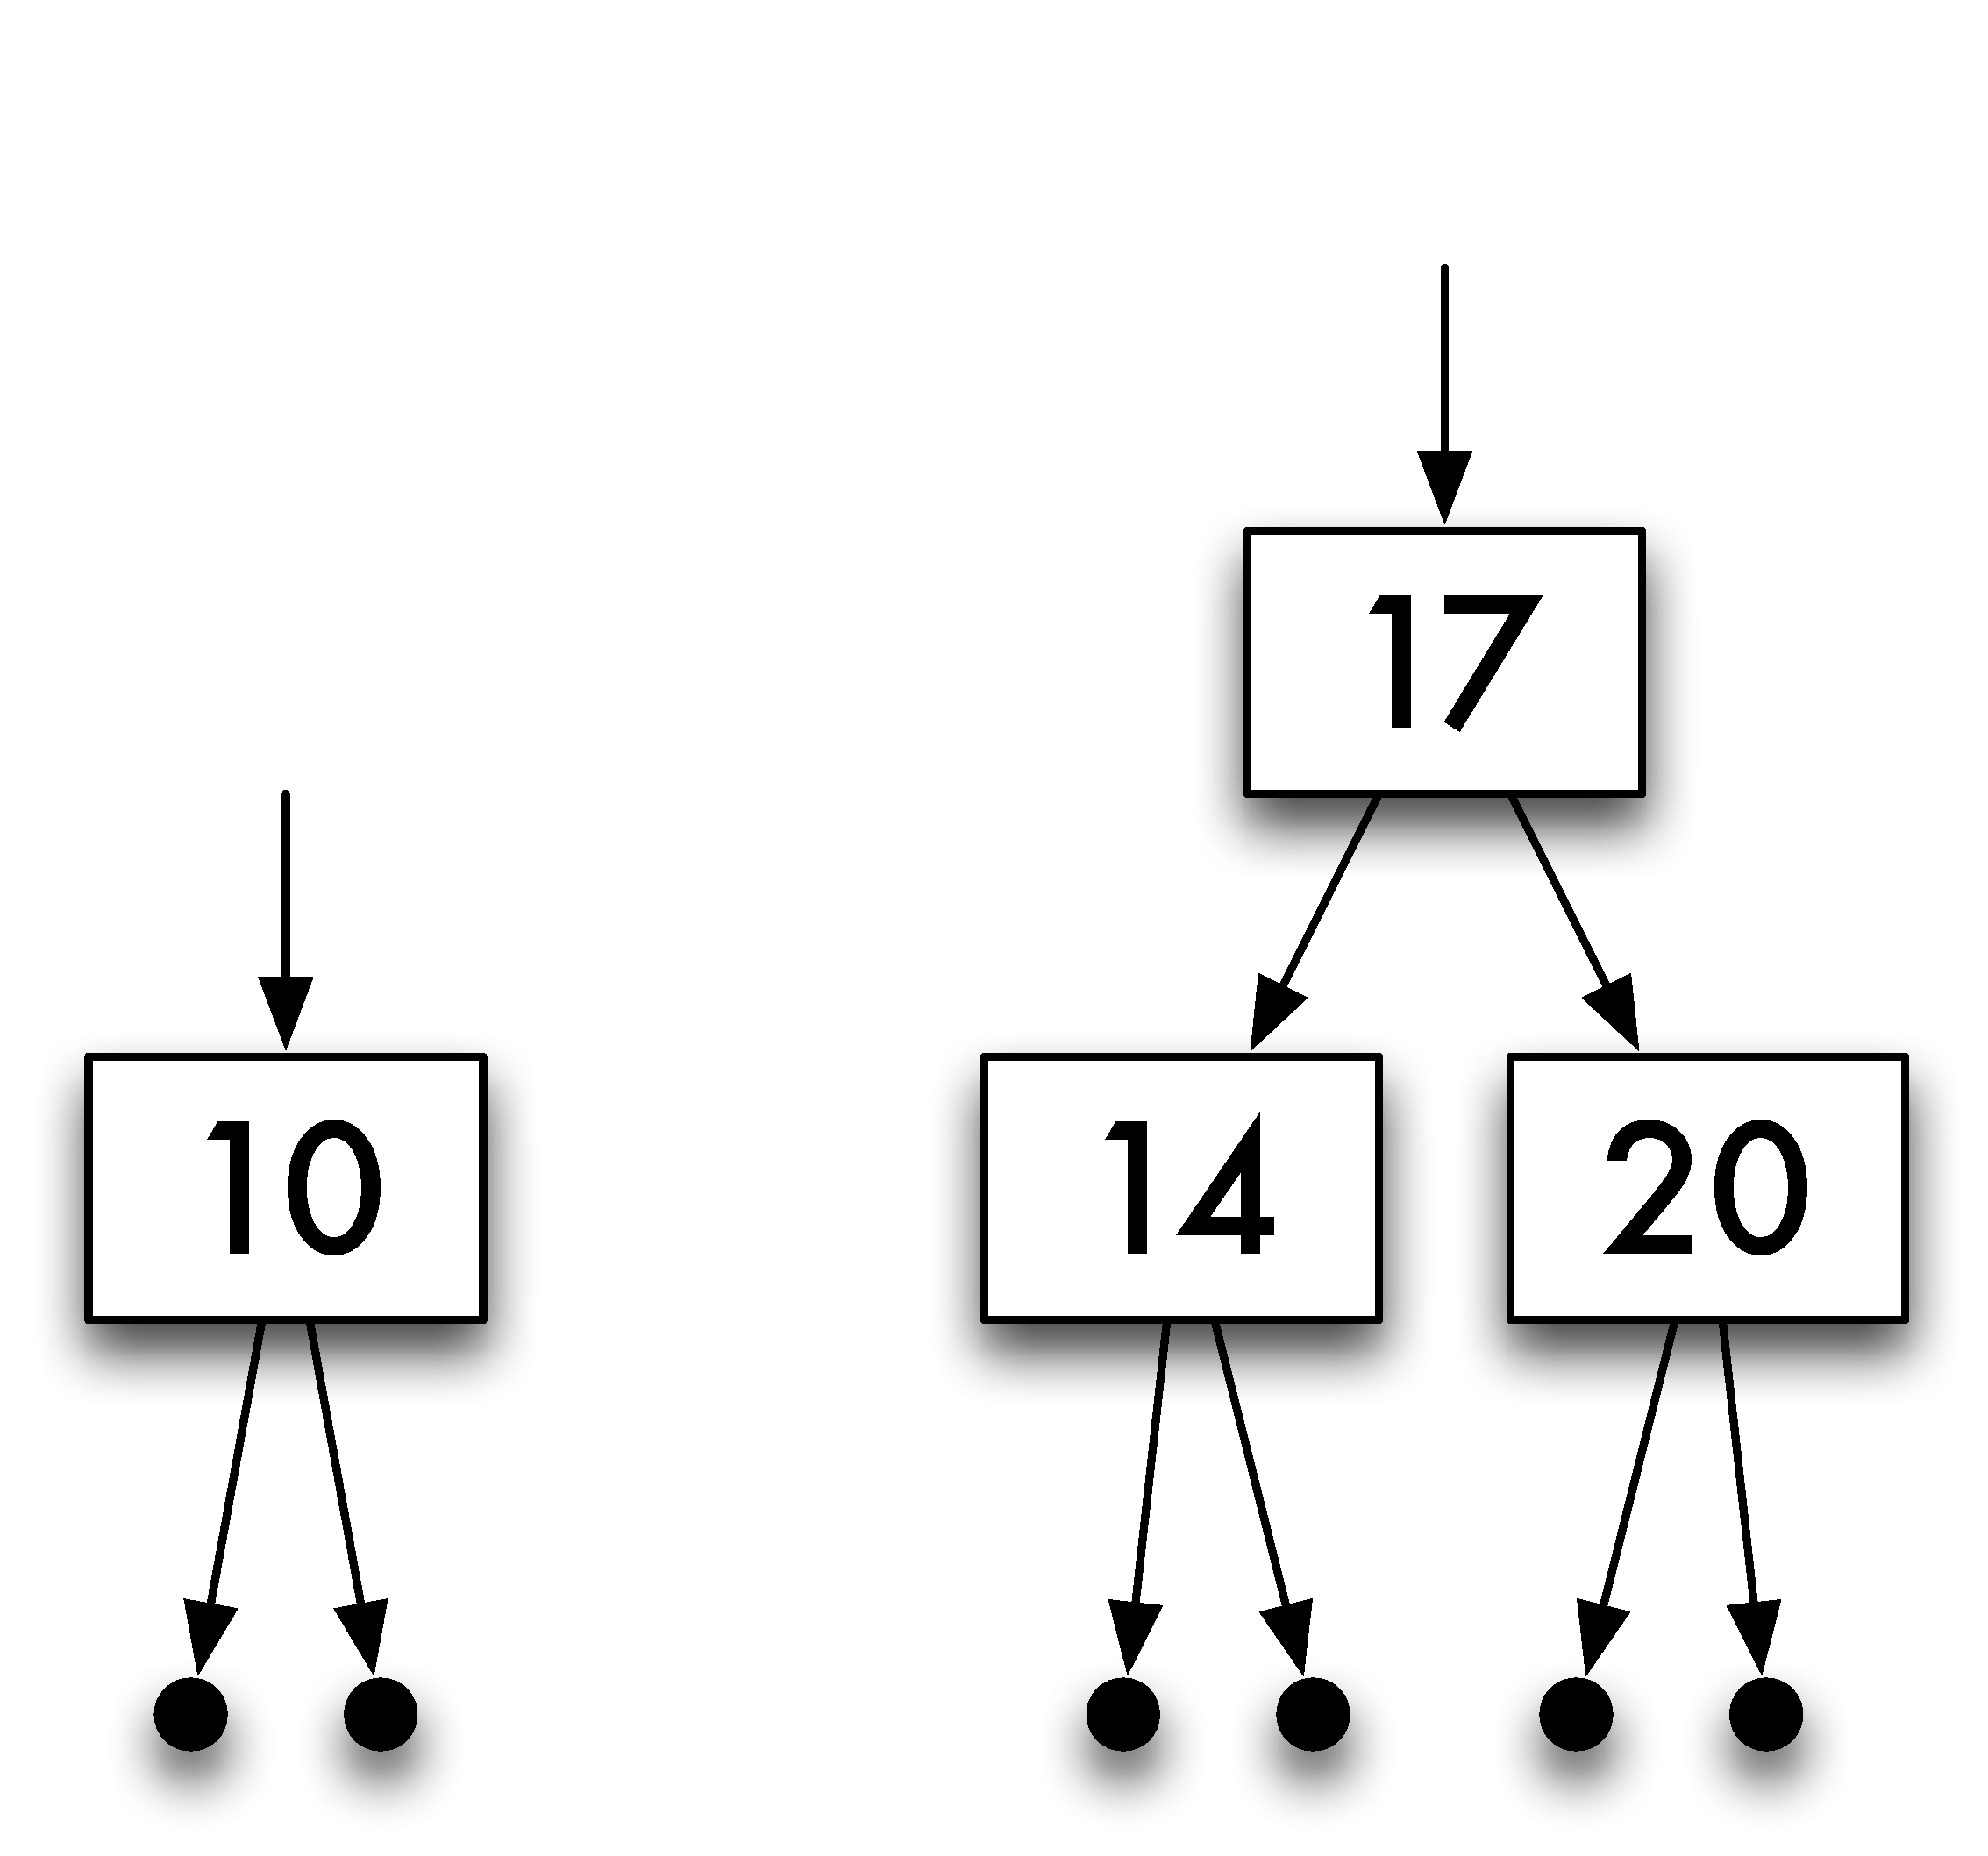
\includegraphics[width=3in]{Pictures/NewTwoTrees.pdf}
\end{center}
\caption{Two trees.}
\label{treeFig2}
\end{figure}
As a Haskell type we
say
\begin{alltt}
data NTree = NilT |\minx{NTree}
             Node Integer NTree NTree
\end{alltt}
Finally, we have already used the type of lists: a list is either empty (
\texttt{[]}) or is built from a head and a tail -- another list -- using the list
constructor `\texttt{:}'. Lists will provide a good guide to using recursive
(and polymorphic) definitions. In particular they suggest how `general'
polymorphic higher-order functions over other algebraic types are defined, and
how programs are verified.  We now look at some examples in more detail.

\subsection*{Expressions}
\index{expression type|see{\texttt{Expr}}}\index{calculator|(}

The type \texttt{Expr} gives a model of the simple numerical expressions discussed
above. These might be used in implementing a simple numerical calculator,
for instance. 
\begin{alltt}\minx{Expr}
data Expr = Lit Integer |
            Add Expr Expr |
            Sub Expr Expr
\end{alltt}
Some examples are

\begin{mytable}
\mi 2 & \mi Lit 2\\
\mi 2+3 & \mi Add (Lit 2) (Lit 3)\\
\mi (3-1)+3 & \mi Add (Sub (Lit 3) (Lit 1)) (Lit 3)  
\end{mytable}

\medskip
\noindent
where the informal expressions are listed in the left-hand column, and their
\texttt{Expr} forms in the right. Given an expression, we might want to
\begin{titemize}
\item evaluate it;
\item turn it into a string, which can then be printed;
\item estimate its size -- count the operators, say.
\end{titemize}
Each of these functions will be defined in the same way, using \textbf{primitive
recursion}.\index{primitive recursion}
As the type is itself recursive, it is not a surprise that the
functions which handle the type are also recursive. Also, the form of the
recursive definitions follows the recursion in the type definition. For
instance, to evaluate an operator expression we work out the values of the
arguments and combine the results using the operator.
\begin{alltt}
eval :: Expr -> Integer\minx{eval}

eval (Lit n)     = n
eval (Add e1 e2) = (eval e1) + (eval e2)
eval (Sub e1 e2) = (eval e1) - (eval e2)
\end{alltt}
Primitive recursive definitions have two parts:
\begin{titemize}
\item At the non-recursive, {\em base\/} cases -- \texttt{(Lit n)} here -- the
value is given outright. 
\index{primitive recursion!base case}
\item At the recursive cases, the values of the function at the
\index{primitive recursion!recursive case}
sub-expressions from which the expression is formed -- \texttt{eval e1} and 
\texttt{eval e2} here -- can be used in
calculating the result. 
\end{titemize}
The \texttt{show} function has a similar form
\begin{alltt}
show :: Expr -> String\index{show@\texttt{show}!\texttt{Expr}}

show (Lit n) = show n
show (Add e1 e2) 
  = "(" ++ show e1 ++ "+" ++ show e2 ++ ")"
show (Sub e1 e2) 
  = "(" ++ show e1 ++ "-" ++ show e2 ++ ")"
\end{alltt}
as does the function to calculate the number of operators in an expression;
we leave this as an exercise. Other exercises at the end of the section look
at a different representation of expressions for which a separate type is used
to represent the different possible operators. Next, we look at another
recursive algebraic type, but after that we return to \texttt{Expr} and give an
example of a non-primitive-recursive definition of a function to rearrange
expressions in a particular way.
\index{calculator|)}

\subsection*{Trees of integers}
\index{tree!numeric}

Trees of integers like that in Figure \ref{treeFig} can be modelled by the type
\begin{alltt}
data NTree = NilT |\minx{NTree}
             Node Integer NTree NTree
\end{alltt}
The null tree is given by \texttt{NilT}, and the trees in Figure \ref{treeFig2}
by
\begin{alltt}
Node 10 NilT NilT
Node 17 (Node 14 NilT NilT) (Node 20 NilT NilT)
\end{alltt}
Definitions of many functions are primitive recursive. For instance,
\index{primitive recursion}
\begin{alltt}
sumTree,depth :: NTree -> Integer\minx{sumTree}\minx{depth}

sumTree NilT           = 0
sumTree (Node n t1 t2) = n + sumTree t1 + sumTree t2

depth NilT             = 0
depth (Node n t1 t2)   = 1 + max (depth t1) (depth t2)
\end{alltt}
with, for example,
\begin{alltt}
sumTree (Node 3 (Node 4 NilT NilT) NilT) = 7
depth   (Node 3 (Node 4 NilT NilT) NilT) = 2
\end{alltt}
As another example, take the problem of finding out how many times a number,
\texttt{p} say, occurs in a tree. The primitive recursion suggests two cases,
depending upon the tree.
\begin{titemize} 
\item For a null tree, \texttt{NilT}, the answer must be zero.
\item For a non-null tree, \texttt{(Node n t1 t2)}, we can find out how many
times \texttt{p} occurs in the sub-trees \texttt{t1} and \texttt{t2} by two recursive
calls; we have to make a case split depending on whether \texttt{p} occurs at the
particular node, that is depending on whether or not \texttt{p==n}. 
\end{titemize}
The final definition is 
\begin{alltt}\minx{occurs}
occurs :: NTree -> Integer -> Integer

occurs NilT p = 0
occurs (Node n t1 t2) p
  | n==p        = 1 + occurs t1 p + occurs t2 p
  | otherwise   =     occurs t1 p + occurs t2 p
\end{alltt}

The exercises at the end of the section give a number of other
examples of functions defined over trees using primitive
recursion. We next look at a particular example where a
different form of recursion is used. 


\subsection*{Rearranging expressions}
%\index{expression type!rearranging}

The next example shows a definition which uses a more general recursion than
we have seen so far. After showing why the generality is necessary, we argue
that the function we have defined is total: it will give a result on all
well-defined expressions.

The operation of addition over the integers
is associative\index{associativity}, so that the way in which an
expression is bracketed is irrelevant to its value. We can, therefore, decide
to bracket expressions involving `\texttt{+}' in any way we choose. The aim here
is to write a program to turn expressions into right bracketed form, as shown in Figure \ref{associate} and
in the following table:
\begin{alltt}
(2+3)+4                 2+(3+4)
((2+3)+4)+5             2+(3+(4+5))
((2-((6+7)+8))+4)+5    (2-(6+(7+8)))+(4+5)
\end{alltt}
What is the program to do? The main aim is to spot occurrences of
\begin{alltt}\minx{Expr}
Add (Add e1 e2) e3 \hfill (AddL)
\end{alltt}
and to transform them to
\begin{alltt}
Add e1 (Add e2 e3)\hfill (AddR)
\end{alltt}
so a first attempt at the program might say
\begin{alltt}
try (Add (Add e1 e2) e3) 
  = Add (try e1) (Add (try e2) (try e3))
try ...
\end{alltt}
which is primitive recursive: on the right-hand side of their definition the
function \texttt{try} is only used on sub-expressions of the argument. This
function will have the effect of transforming \texttt{(AddL)} to \texttt{(AddR)}, but
unfortunately 
\texttt{(AddExL)} will be sent to \texttt{(AddExR)}:
\begin{alltt}
((2+3)+4)+5 \hfill (AddExL) 
(2+3)+(4+5)\hfill (AddExR)  
\end{alltt}

\begin{figure}[t]
\begin{center}
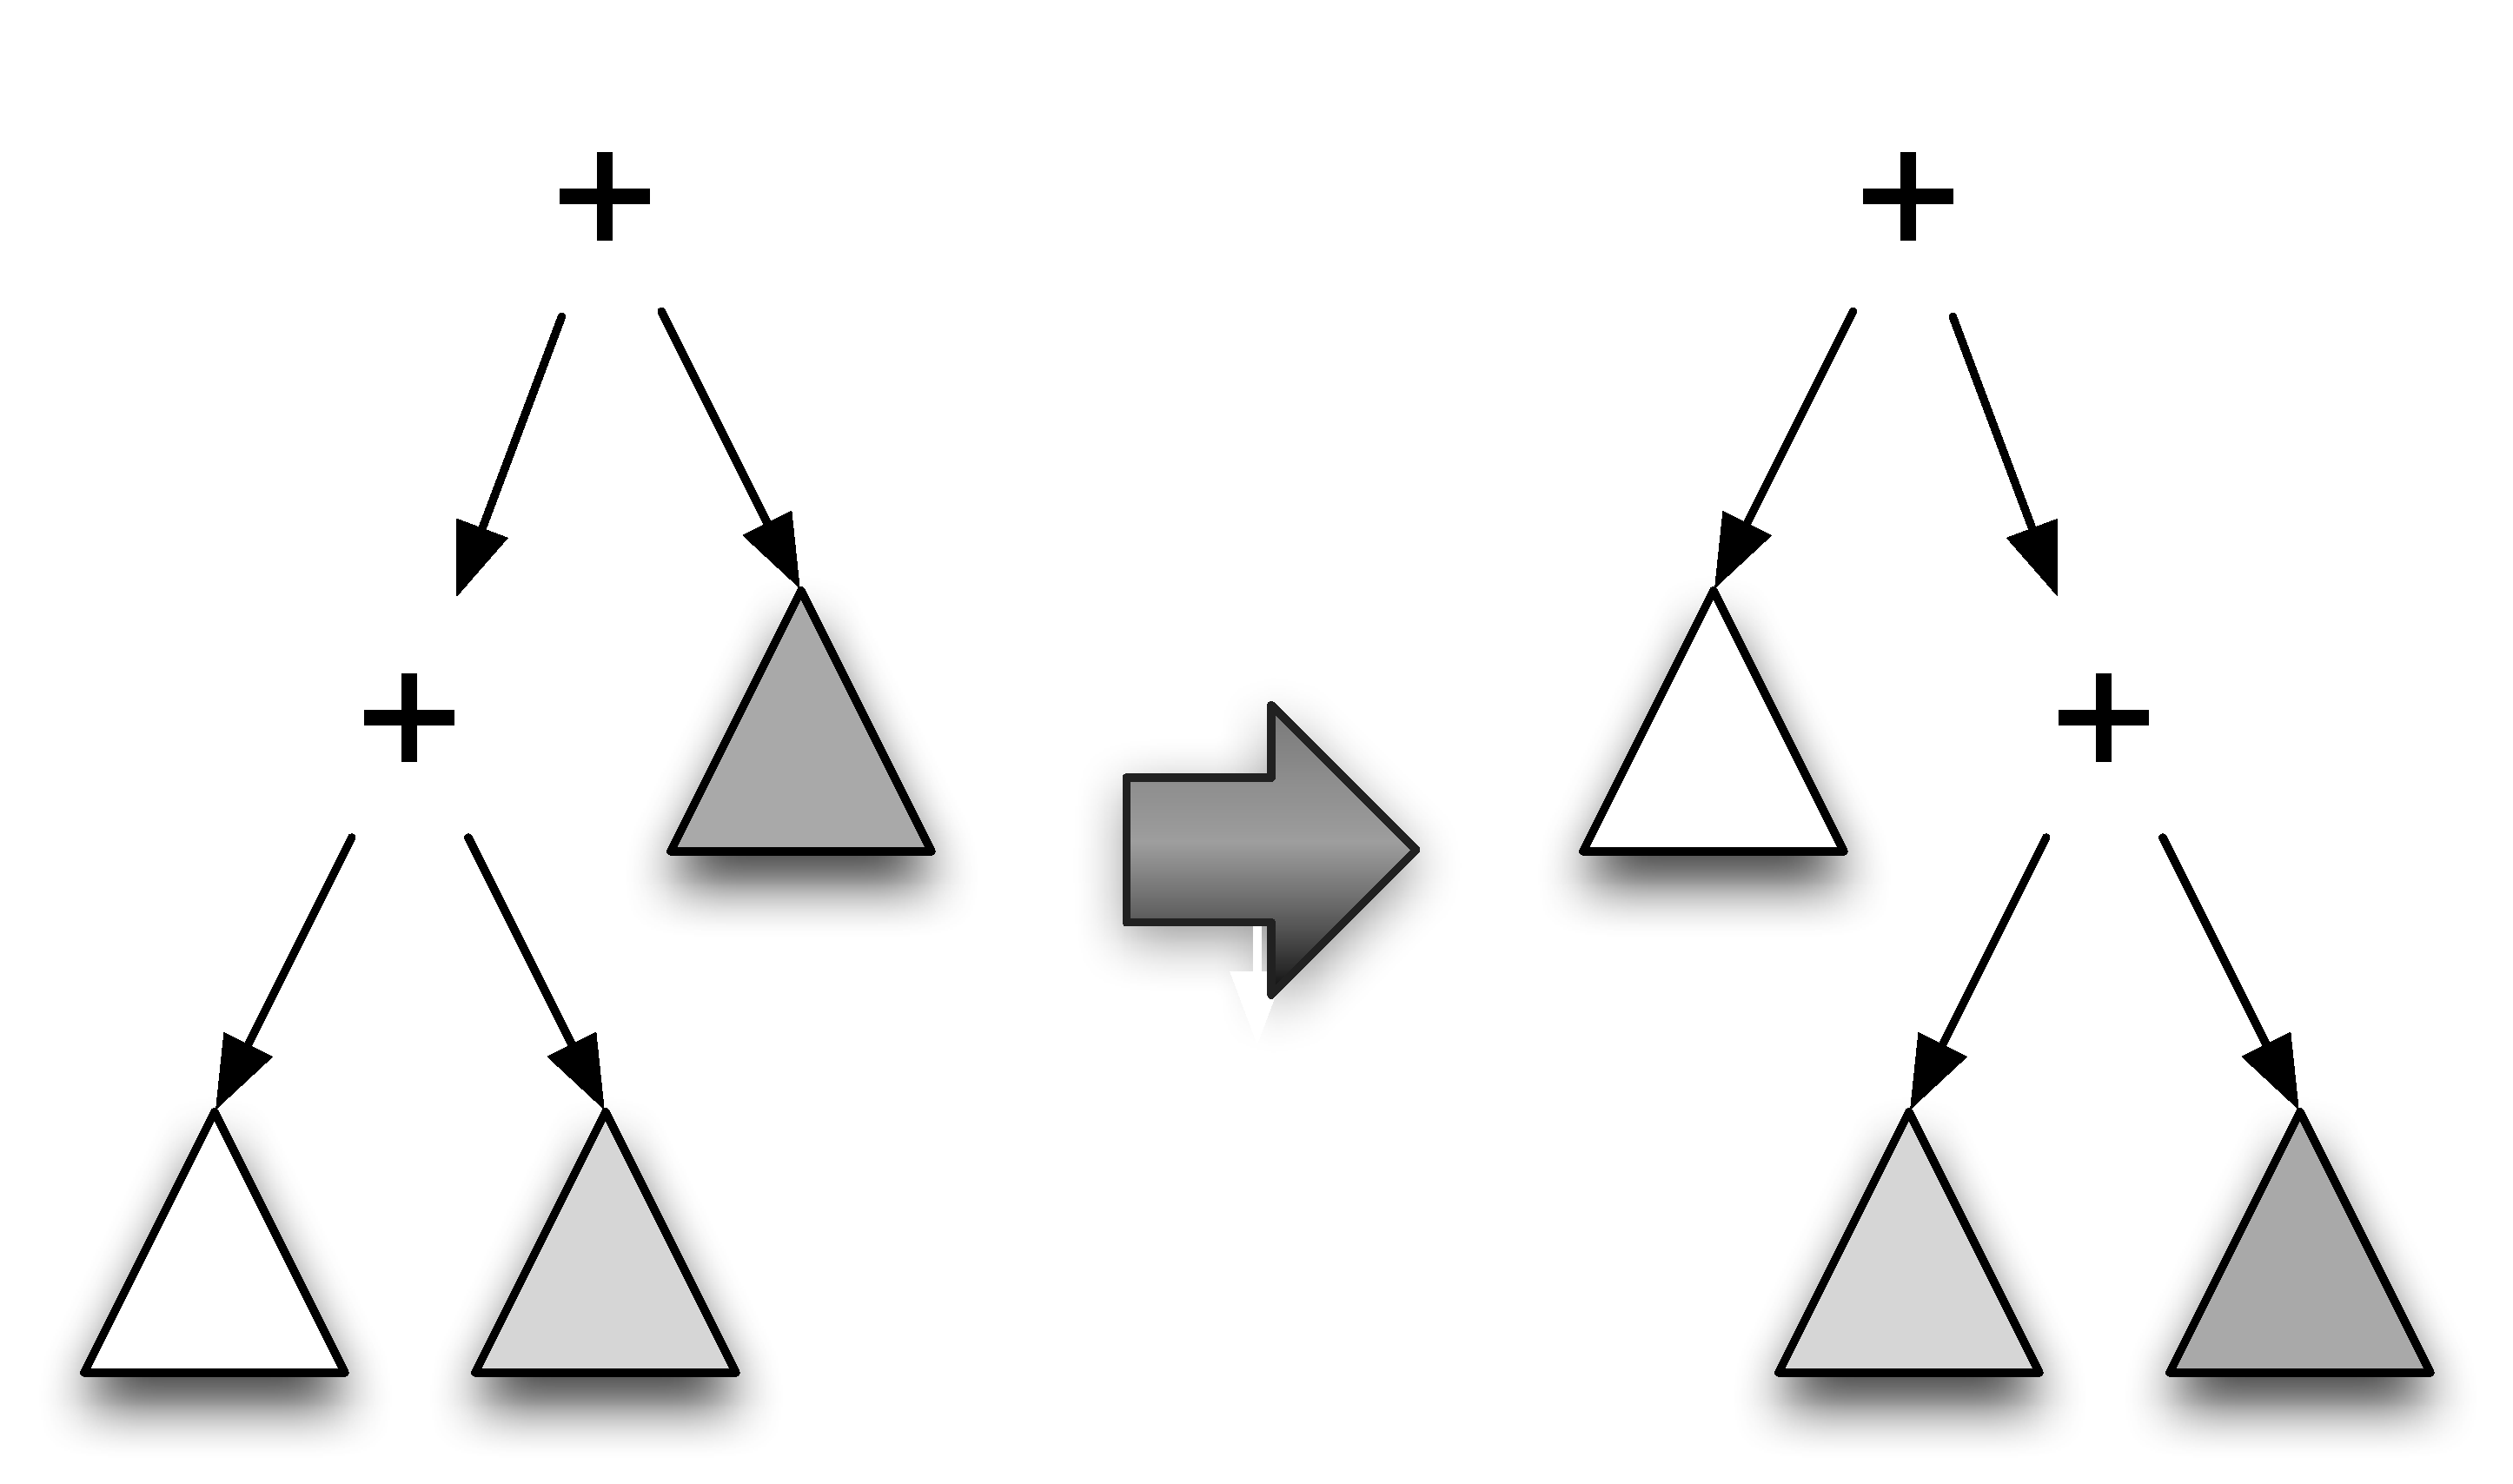
\includegraphics[width=3in]{Pictures/Associate.pdf}
\end{center}
\caption{Rearranging additions}
\label{associate}
\end{figure}

\noindent
The problem is that
in transforming \texttt{(AddL)} to \texttt{(AddR)} we may produce another pattern we are
looking for at the top level: this is precisely what happens when \texttt{(AddExL)}
is transformed to \texttt{(AddExR)}. We therefore have to call the function {\em again\/} on the
result of the rearrangement
\begin{alltt}
assoc :: Expr -> Expr\minx{assoc}

assoc (Add (Add e1 e2) e3)
  = assoc (Add e1 (Add e2 e3)) \hfill (Add.1)
\end{alltt}
The other cases in the definition make sure that the {\em parts\/} of an
expression are rearranged as they should be.
\begin{alltt}
assoc (Add e1 e2) 
  = Add (assoc e1) (assoc e2) \hfill (Add.2)
assoc (Sub e1 e2) 
  = Sub (assoc e1) (assoc e2)
assoc (Lit n) 
  = Lit n
\end{alltt}
The equation \texttt{(Add.2)} will only be applied to the cases where \texttt{(Add.1)} does
not apply -- this is when \texttt{e1} is either a \texttt{Sub} or a \texttt{Lit}
expression. This is always the case in pattern matching\index{pattern matching}; the {\em first\/}
applicable equation is used.

When we use primitive recursion we can be sure that the recursion will {\bf
terminate}\index{termination}
to give an answer: the  recursive calls are only made on smaller
expressions and so, after a finite number of calls to the function, a base
case will be reached. 

The \texttt{assoc} function is more complicated, and we
need a more subtle argument to see that the function will always give a
result. The equation \texttt{(Add.1)} is the tricky one, but intuitively, we can see
that some progress has been made -- some of the `weight' of the tree has moved
from left to right. In particular, one addition symbol has swapped sides.
None of the other equations moves a plus in the other direction, so
that after applying \texttt{(Add.1)} a finite number of times, there will be no more
exposed addition symbols at the top level of the left-hand side. This means
that the recursion cannot go on indefinitely, and so the function always
leads to a result.

In Section \ref{proofAlgTypes} we'll look at specifying QuickCheck properties for functions over algebraic types, including \texttt{assoc}, as well as showing how some of these can be proved by induction.

\subsection*{Syntax: infix constructors}
\index{constructor!infix}

We have seen that functions can be written in infix form; this also applies to
constructors. We can, for example, redefine the function \texttt{assoc} thus:
\begin{alltt}
assoc ((e1 `Add` e2) `Add` e3)
  = assoc (e1 `Add` (e2 `Add` e3))
 ...
\end{alltt}
using the infix form of the constructor, given by surrounding it with
back-quotes. 

When an expression like this is \texttt{show}n, it appears in prefix
form, so that the expression \texttt{(Lit 3) `Add` (Lit 4)} appears as
\begin{alltt}
Add (Lit 3) (Lit 4)
\end{alltt}
In a \texttt{data}
definition we can define Haskell operators which are themselves constructors. 
These constructors have the same syntax as
operator symbols, except that their first character must be a `\texttt{:}', which
is reminiscent of `\texttt{:}', itself an infix constructor. For our type of
integer expressions, we might define
\begin{alltt}
data Expr = Lit Integer |
            Expr :+: Expr |
            Expr :-: Expr
\end{alltt}
When an expression involving operator constructors is printed, the
constructors appear in the infix position, unlike the quoted constructors
above.

It is left as an exercise to complete the redefinition of functions over 
\texttt{Expr} under this redefinition of the \texttt{Expr} type.

\subsection*{Mutual recursion}
\index{recursion!mutual}
\index{recursive type!mutually recursive}

In describing one type, it is often useful to use others; these in turn may
refer back to the original type: this gives a pair of \textbf{mutually
recursive} types. A description of a person might include biographical
details,
which in turn might refer to other people. For instance: 
\begin{alltt}
data Person = Adult Name Address Bio |
              Child Name
data Bio    = Parent String [Person] |
              NonParent String
\end{alltt}
In the case of a
parent, the biography contains some text, as well as a list of their children,
as elements of the type \texttt{Person}.

Suppose that we want to define a function which shows information about a person as
a string. Showing this information will require us to show some biographical
information, which itself contains further information about people. We thus have two
mutually recursive functions:
\begin{alltt}
showPerson (Adult nm ad bio) 
  = show nm ++ show ad ++ showBio bio
  ...
showBio (Parent st perList)
  = st ++ concat (map showPerson perList)
  ...
\end{alltt}
\index{calculator|(}
\begin{exercises}

\item
Give calculations of 
\begin{alltt}
eval (Lit 67)
eval (Add (Sub (Lit 3) (Lit 1)) (Lit 3))
show (Add (Lit 67) (Lit (-34)))
\end{alltt}

\item
Define the function
\begin{alltt}
size :: Expr -> Integer
\end{alltt}
which counts the number of operators in an expression.

\item
Add the operations of multiplication and integer division to the type 
\texttt{Expr}, and redefine the functions \texttt{eval}, \texttt{show} and \texttt{size}
to include these new cases. What does your definition of \texttt{eval} do when
asked to perform a division by zero?

\item
Instead of adding extra constructors to the \texttt{Expr} type, as in the
previous question, it is possible to factor the definition thus:

\label{modExpr}\begin{alltt}
data Expr = Lit Integer |\minx{Expr}
            Op Ops Expr Expr

data Ops  = Add | Sub | Mul | Div \minx{Ops}
\end{alltt}
Show how the functions \texttt{eval}, \texttt{show} and \texttt{size} are defined
for this type, and discuss the changes you have to make to your definitions if
you add the extra operation \texttt{Mod} for remainder on integer division.

\item
Give line-by-line calculations of 
\begin{alltt}
sumTree (Node 3 (Node 4 NilT NilT) NilT)
depth   (Node 3 (Node 4 NilT NilT) NilT)
\end{alltt}

\item
Complete the redefinition of functions over \texttt{Expr} after it has been
defined using the infix constructors \texttt{:+:} and \texttt{:-:}.

\item
Define functions to return the left- and right-hand sub-trees
of an \texttt{NTree}.

\item
Define a function to decide whether a number is an element of an \texttt{NTree}.

\item
Define functions to find the maximum and minimum values held in an 
\texttt{NTree}.

\item
A tree is reflected by swapping left and right sub-trees, recursively. Define\break
a function to reflect an \texttt{NTree}. What is the result of
reflecting twice,\break \texttt{reflect .\ reflect}?

\item
Define functions
\begin{alltt}
collapse, sort :: NTree -> [Integer]
\end{alltt}
which turn a tree into a list. The function \texttt{collapse} should enumerate the
left sub-tree, then the value at the node and finally the right sub-tree;
\texttt{sort} should sort the elements in ascending order. For instance, 
\begin{alltt}
collapse (Node 3 (Node 4 NilT NilT) NilT) = [4,3]
sort     (Node 3 (Node 4 NilT NilT) NilT) = [3,4]
\end{alltt}

\item
Complete the definitions of \texttt{showPerson} and \texttt{showBio} which were
left incomplete in the text.

\item
It is possible to extend the type \texttt{Expr} so that it contains
{\em conditional \/}
expressions, \texttt{If b e1 e2},
where \texttt{e1} and \texttt{e2} are expressions, and
\texttt{b} is a Boolean expression, a member of the type \texttt{BExp},
\begin{alltt}
data Expr = Lit Integer |\minx{Expr}
            Op Ops Expr Expr |
            If BExp Expr Expr
\end{alltt}
The expression
\begin{alltt}
If b e1 e2
\end{alltt}
has the value of \texttt{e1} if \texttt{b} has the
value \texttt{True} and otherwise it has the value of \texttt{e2}.
\begin{alltt}
data BExp = BoolLit Bool |\minx{BExp}
            And BExp BExp |
            Not BExp |
            Equal Expr Expr |
            Greater Expr Expr
\end{alltt}
The five clauses here give
\begin{titemize}
\item Boolean literals, \texttt{BoolLit True} and \texttt{BoolLit False}.
\item The conjunction of two expressions; it is \texttt{True} if both sub-expressions have
the value \texttt{True}.
\item The negation of an expression. \texttt{Not be} has value \texttt{True} if
\texttt{be} has the value \texttt{False}.
\item \texttt{Equal e1 e2} is \texttt{True} when the two numerical expressions have
equal values.
\item \texttt{Greater e1 e2} is \texttt{True} when the numerical expression 
\texttt{e1} has a larger value then \texttt{e2}.
\end{titemize}
Define the functions 
\begin{alltt}
eval  :: Expr -> Integer \minx{eval}
bEval :: BExp -> Bool\minx{bEval}
\end{alltt}
by mutual recursion, and
extend the function \texttt{show} to show the redefined type of expressions.
\index{recursive type|)}
\index{calculator|)}
\end{exercises}
\section{Polymorphic algebraic types}
\label{polyAlg}
\index{algebraic type!polymorphic|(}


Algebraic type definitions can contain the type variables \texttt{a}, \texttt{b}
and so on, defining polymorphic types. The definitions are as before, with the
type variables used in the definition appearing after the type name on the 
left-hand side of the definition. A simple example is
\begin{alltt}
data Pairs a = Pr a a\minx{Pairs}
\end{alltt}
and example elements of the type are
\begin{alltt}
Pr 2 3    :: Pairs Integer
Pr [] [3] :: Pairs [Int]
Pr [] []  :: Pairs [a]
\end{alltt}
A function to test the equality of the two halves of a pair is given by
\begin{alltt}\minx{equalPair}
equalPair :: Eq a => Pairs a -> Bool
equalPair (Pr x y) = (x==y)
\end{alltt}
The remainder of this section explores a sequence of further examples.

\subsection*{Lists}
\index{lists!algebraic type of}


The built-in type of lists can be given by a definition like
\begin{alltt}\minx{List}\minx{:::}
infixr 5 :::

data List a = NilL | a ::: (List a)
              deriving (Eq,Ord,Show,Read)
\end{alltt}
where the syntax \texttt{[a]}, \texttt{[]} and `\texttt{:}' is used for \texttt{List a},
\texttt{NilList} and \texttt{:::}. Note that we have given a \textbf{fixity declaration} for \texttt{:::} to give it the same fixity and associativity as \texttt{:}, we can therefore write expressions like this:\index{fixity!declaration}
\begin{alltt}
\textsl{*Chapter14>} 2+3 ::: 4+5 ::: NilL
\textsl{5 ::: (9 ::: NilL)}
\end{alltt}
much as lists are written with \texttt{:}.

Lists form a useful paradigm
for recursive polymorphic types. In particular, we can see the possibility of
defining useful families of functions over such types, and the way in which
program verification can proceed by induction over the structure of a type.

\subsection*{Binary trees}
\index{tree!binary}\index{binary tree|see{tree}}

The trees of Section \ref{recTypes} carry numbers at each node; there is
nothing special about numbers, and we can equally well say that
they have elements of an arbitrary type at the nodes:
\begin{alltt}\minx{Nil}\minx{Node}
data Tree a = Nil | Node a (Tree a) (Tree a)\minx{Tree}
              deriving (Eq,Ord,Show,Read)
\end{alltt}
The definitions of \texttt{depth} and \texttt{occurs} carry over unchanged:
\begin{alltt}
depth :: Tree a -> Integer\minx{depth}
depth Nil            = 0
depth (Node n t1 t2) = 1 + max (depth t1) (depth t2)
\end{alltt}
as do many of the functions defined in the exercises at the end of Section
\ref{recTypes}.  
One of these is the function collapsing a tree into a list. This is done
by visiting the elements of the tree `inorder', that is visiting first the left
sub-tree, then the node itself, then the right sub-tree, thus:
\begin{alltt}
collapse :: Tree a -> [a]\minx{collapse}
collapse Nil = []
collapse (Node x t1 t2)
  = collapse t1 ++ [x] ++ collapse t2
\end{alltt}
For example,
\begin{alltt}
collapse (Node 12 
               (Node 34 Nil Nil) 
               (Node 3 (Node 17 Nil Nil) Nil))
  = [34,12,17,3]
\end{alltt}
Various higher-order functions are definable, also,
\begin{alltt}
mapTree :: (a -> b) -> Tree a -> Tree b\minx{mapTree}
mapTree f Nil = Nil
mapTree f (Node x t1 t2)
  = Node (f x) (mapTree f t1) (mapTree f t2)
\end{alltt}
We shall return to trees in Section \ref{srchTrees}, where
particular `search' trees form a case study.


\subsection*{The union type, \texttt{Either}}
\index{union type}\index{sum type}

Type definitions can take more than one parameter. We saw earlier the example
of the type whose elements were either a name or a number. In general we can
form a type whose elements come either from \texttt{a} or from \texttt{b}:
\begin{alltt}\minx{Left}\minx{Right}
data Either a b = Left a | Right b
                  deriving (Eq,Ord,Read,Show)\minx{Either}
\end{alltt}
Members of the `union' or `sum' type are \texttt{(Left x)}, with
\texttt{x::a}, and
\texttt{(Right y)} with \texttt{y::b}. The `name or number' type is given by 
\texttt{Either String Int} and
\begin{alltt}
Left "Duke of Prunes" :: Either String Int
Right 33312           :: Either String Int
\end{alltt}
We can tell whether an element is in the first half of the 
union by\minx{isLeft}
\begin{alltt} 
isLeft :: Either a b -> Bool
isLeft (Left _)  = True
isLeft (Right _) = False
\end{alltt}
To define a function from \texttt{Either a b} to \texttt{Int}, say, we have to deal
with two cases,
\begin{alltt}
fun :: Either a b -> Int
fun (Left x)  = ... x ...
fun (Right y) = ... y ...
\end{alltt}
In the first case, the right-hand side takes \texttt{x} to an \texttt{Int}, so is
given by
a function from \texttt{a} to \texttt{Int}; in the second case \texttt{y} is taken to
an \texttt{Int}, thus being given by a function from \texttt{b} to \texttt{Int}. 

Guided by this, we can give a higher-order
function which {\em joins together\/} two functions defined on \texttt{a} and 
\texttt{b} to a function on \texttt{Either a b}. The definition follows, and is
illustrated in Figure \ref{either}.
\begin{figure}[t]
\begin{center}
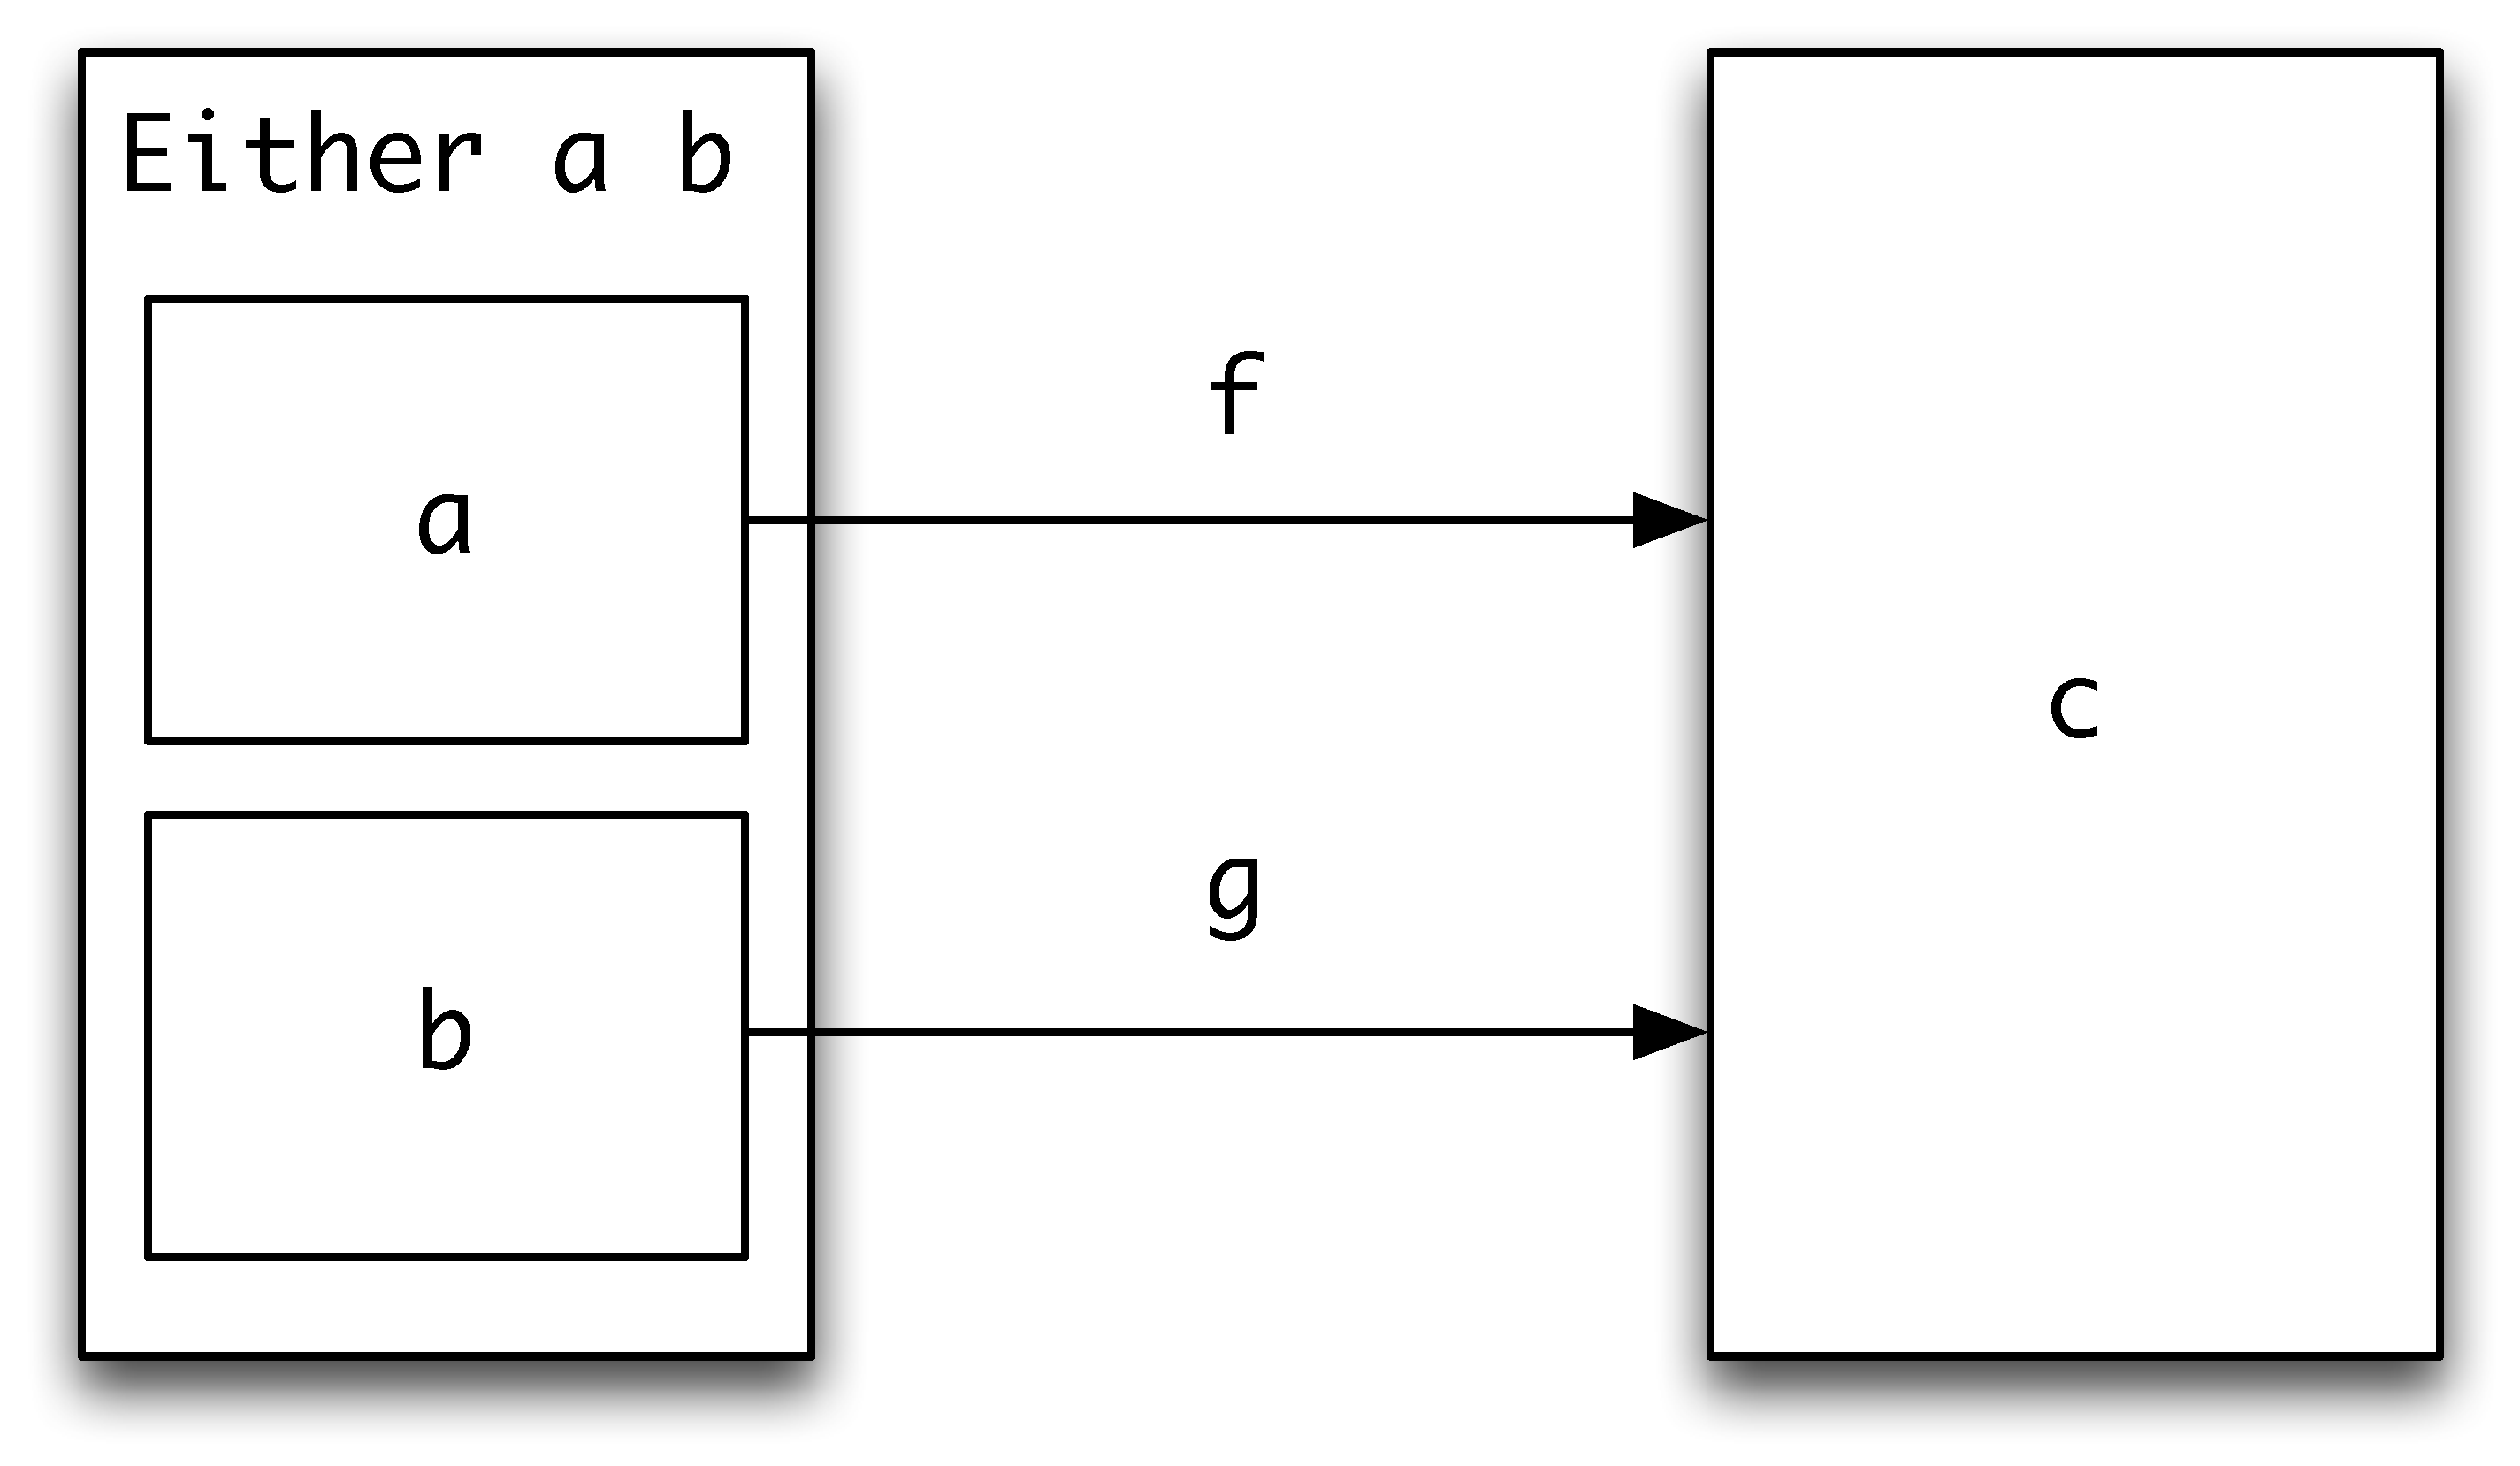
\includegraphics[width=3in]{Pictures/either1}
\end{center}
\label{either}
\caption{Joining together functions.}
\end{figure} 
\begin{alltt}\minx{either}
either :: (a -> c) -> (b -> c) -> Either a b -> c

either f g (Left x)  = f x
either f g (Right y) = g y
\end{alltt}
If we have a function \texttt{f::a -> c} and we wish to apply it to an element
of \mbox{\texttt{Either a b}}, there is a problem: what do we do if the element is
in the right-hand side of the \texttt{Either} type? 
A simple answer is to raise an \texttt{error}
\begin{alltt}\minx{applyLeft}
applyLeft :: (a -> c) -> Either a b -> c
applyLeft f (Left x)  = f x
applyLeft f (Right _) = error "applyLeft applied to Right"
\end{alltt}
but in the next section we shall explore other ways of handling errors in more
detail.

\index{algebraic type!polymorphic|)}
\begin{exercises}

\item
Investigate which of the functions over trees discussed in the exercises of
Section \ref{recTypes} can be made polymorphic.

\item
Define a function \texttt{twist} which swaps the order of a union
\begin{alltt}
twist :: Either a b -> Either b a
\end{alltt}
What is the effect of \texttt{(twist .\ twist)}?

\item
How would you define \texttt{applyLeft} using the function
\texttt{either}?

\item
Show that any function of type \texttt{a -> b} can be transformed into
functions of type
\begin{alltt}
a -> Either b c
a -> Either c b
\end{alltt}

\item
How could you generalize \texttt{either} to \texttt{join} so that it has type
\begin{alltt}
join :: (a -> c) -> (b -> d) -> Either a b -> Either c d
\end{alltt}
You might find the answer to the previous exercise useful here, if you want
to define \texttt{join} using \texttt{either}.
\end{exercises}

\medskip\noindent
The trees defined in the text are {\em binary}: each non-nil
tree has exactly two
sub-trees. We can instead define general
trees with an arbitrary list of sub-trees,
thus:
\begin{alltt}
data GTree a = Leaf a | Gnode [GTree a]\minx{GTree}
\end{alltt}
The exercises which follow concern these trees.

\begin{exercises}
\item
Define functions 
\begin{titemize} 
\item to count the number of leaves in a \texttt{GTree}; 
\item to find
the depth of a \texttt{GTree}; 
\item to sum a numeric \texttt{GTree Int}; 
\item to find whether
an element appears in a \texttt{GTree}; 
\item to map a function over the elements at
the leaves of a \texttt{GTree}; and 
\item to flatten a \texttt{GTree} to a list.
\end{titemize}
In each case give the type of the function that you have defined.
\item
How is the completely empty tree represented as a \texttt{GTree}?

\end{exercises}
\section{Modelling program errors}
\label{progErrs}
\index{error handling|(}

\noindent
How should a program deal with a situation which ought not to occur? Examples
of such situations include
\begin{titemize}
\item attempts to divide by zero, to take the square root of a negative
number, and other arithmetical transgressions;
\item attempts to take the head of an empty list -- this is a special case
of a definition over an algebraic type from which one case (here the empty
list) is absent.
\end{titemize}
This section examines the problem, giving three approaches of increasing
sophistication. The simplest method is to stop computation  and to report the
source of  the problem. This is indeed what the Haskell system does in the
cases listed above, and we can do this in functions we define ourselves using
the \texttt{error} function,
\begin{alltt}
error :: String -> a\minx{error}
\end{alltt}
An attempt to evaluate the expression 
\texttt{error "Circle with negative radius"}
in GHCi results in the message 
\begin{alltt}
*** Exception: Circle with negative radius
\end{alltt}
being printed and computation stopping.

The problem with this approach is that all the useful information in the
computation is lost; instead of this, the error can be dealt with in some way
{\em without\/} stopping computation completely. Two approaches suggest
themselves, and we look at them in turn now.

\subsection*{Dummy values}
\index{dummy values at errors}

The function \texttt{tail} is supposed to give the tail of a list, and it gives an
error message on an empty list:
\begin{alltt}
tail :: [a] -> [a]\minx{tail}
tail (_:xs) = xs
tail []     = error "Prelude.tail: empty list"
\end{alltt}
We could redefine it to say
\begin{alltt}
tl :: [a] -> [a]\minx{tl}
tl (_:xs) = xs
tl []     = []
\end{alltt}
Now, an attempt to take the tail of {\em any\/} list will succeed. In a
similar way we could say
\begin{alltt}
divide :: Integer -> Integer -> Integer
divide n m 
  | (m /= 0)    = n `div` m
  | otherwise   = 0
\end{alltt}
so that division by zero gives some answer. For \texttt{tl} and \texttt{divide}
there have been obvious choices about what the value in the `error' case
should be; for \texttt{head} there is not, and instead we can supply an extra
parameter to \texttt{head}, which is to be used in the case of the list being
empty.
\begin{alltt}\minx{hd}
hd :: a -> [a] -> a
hd y (x:_) = x
hd y []    = y
\end{alltt}
This approach is completely general; if a function \texttt{f} (of one
argument, say) usually raises an error when \texttt{cond} is \texttt{True}, we can
define a new function
\begin{alltt}
fErr y x 
  | cond        = y
  | otherwise   = f x
\end{alltt}
This approach works well in many cases; the only drawback is that we have no
way of telling when an error has occurred, since we may get the result 
\texttt{y} from either the error or the `normal' case.
Alternatively we can use an error type to trap and process errors; this
we look at now.

\subsection*{Error types}
\index{error handling!error type}
\minx{Maybe}

The previous approach works by returning a dummy value when an error has
occurred. Why not instead return an error {\em value\/} as a result? We
define the type
\begin{alltt}\minx{Nothing}\minx{Just}
data Maybe a = Nothing | Just a\minx{Maybe}
               deriving (Eq,Ord,Read,Show)
\end{alltt}
which is effectively the type \texttt{a} with an extra value \texttt{Nothing} added.
We can now define a division function \texttt{errDiv} thus
\begin{alltt}\minx{errDiv}
errDiv :: Integer -> Integer -> Maybe Integer
errDiv n m 
  | (m /= 0)    = Just (n `div` m)
  | otherwise   = Nothing 
\end{alltt}
and in the general case, where \texttt{f} gives an error when \texttt{cond} holds,
\begin{alltt}
fErr x 
  | cond        = Nothing
  | otherwise   = Just (f x)
\end{alltt}
The results of these functions are now not of the original output type, \texttt{a}
say, but
of type \texttt{Maybe a}. These \texttt{Maybe} types allow us to \textbf{raise} an error,
potentially. We can do two things with a potential error which has been 
raised
\begin{titemize}
\item we can {\em transmit\/} the error through a function, the effect
of \texttt{mapMaybe};\minx{mapMaybe}
\index{error handling!error transmission}
\item we can {\em trap\/} an error, the role of \texttt{maybe}.
\index{error handling!error trapping}\minx{maybe}
\end{titemize}
These two operations are illustrated in Figure \ref{errPic}, and we define them now.

The function \texttt{mapMaybe} transmits an error value through the application of
the function \texttt{g}. Suppose that \texttt{g} is a function of type \texttt{a -> b}, and that
we are to lift it to operate on the type \texttt{Maybe a}. In the case
of an argument
\texttt{Just x}, \texttt{g} can be
applied to the \texttt{x} to give a result, \texttt{g x}, of type \texttt{b}; this is put 
into \texttt{Maybe b}
by applying  the constructor function \texttt{Just}. On the other hand, if \texttt{Nothing} is the argument then 
\texttt{Nothing} is the result.
\begin{alltt}
mapMaybe :: (a -> b) -> Maybe a -> Maybe b\minx{mapMaybe}

mapMaybe g Nothing  = Nothing
mapMaybe g (Just x) = Just (g x)
\end{alltt}
In trapping an error, we aim to return a result of type \texttt{b}, from an
input of type \texttt{Maybe a}; we have two cases to deal with
\begin{titemize}
\item in the \texttt{Just} case, we apply a function from \texttt{a} to \texttt{b};
\item in the \texttt{Nothing} case, we have to give the value of type \texttt{b} which
is to be returned. (This is rather like the value we
supplied to \texttt{hd} earlier.)
\end{titemize}
The higher-order function which achieves this
is \texttt{maybe}, whose arguments \texttt{n} and \texttt{f} are used in the \texttt{Nothing}
and \texttt{Just} cases respectively. 
\begin{figure}[t]
\begin{center}
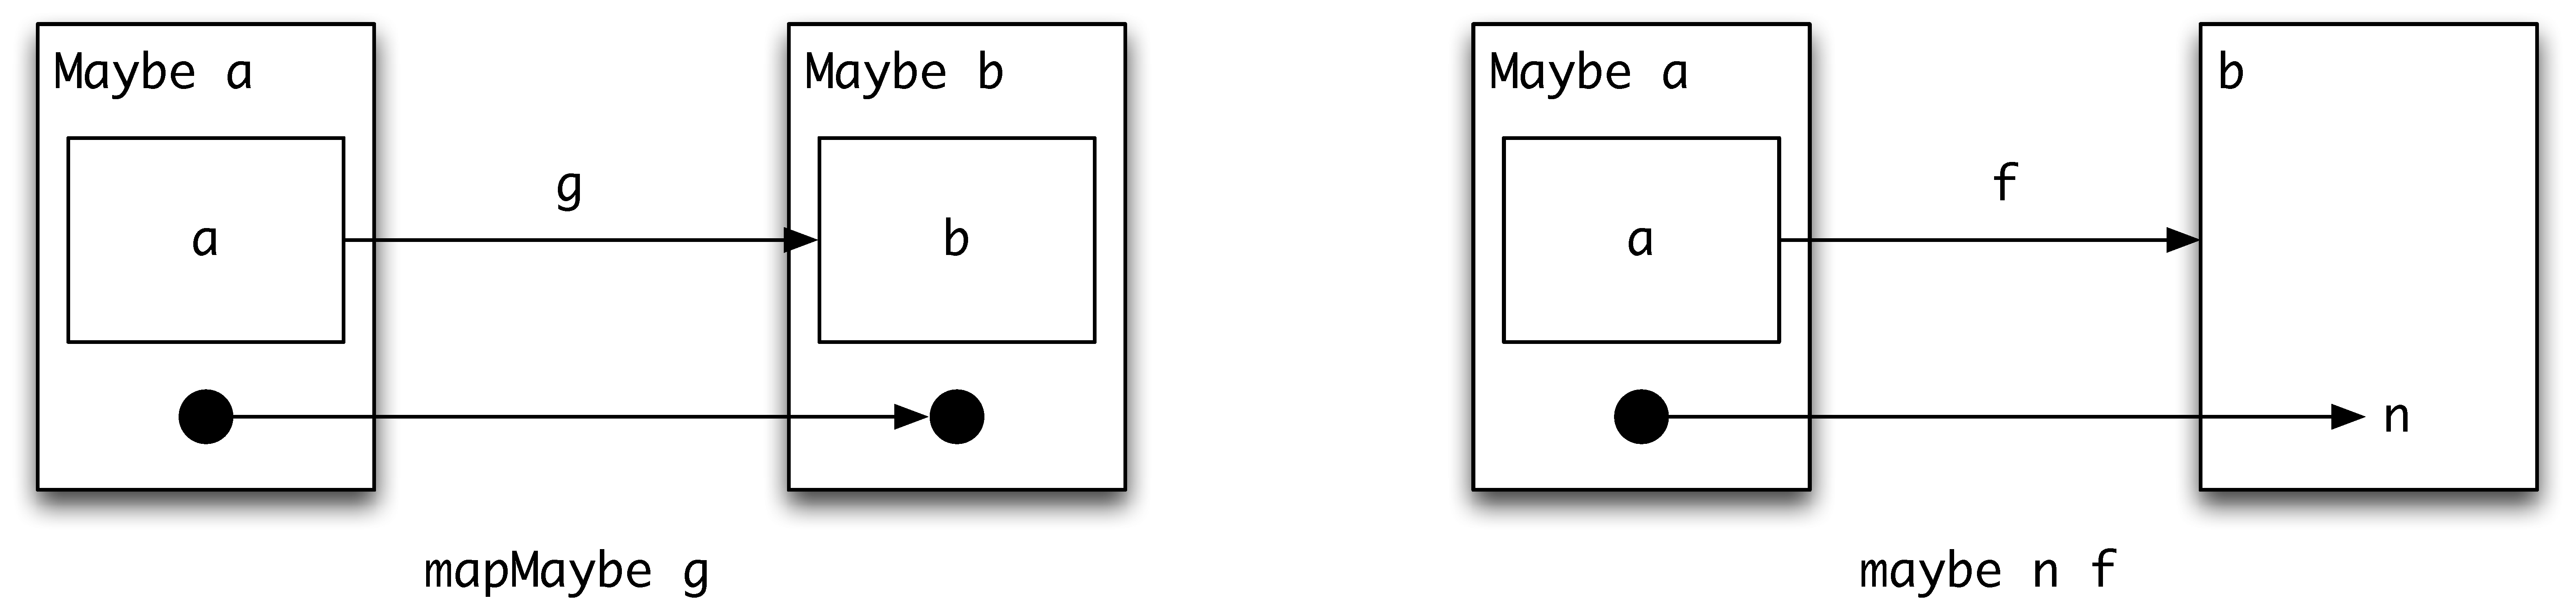
\includegraphics[width=5in]{Pictures/maybe1.pdf}
\end{center}
\label{errPic}
\caption{Error-handling functions.}
\end{figure}
\begin{alltt}
maybe :: b -> (a -> b) -> Maybe a -> b\minx{maybe}

maybe n f Nothing  = n
maybe n f (Just x) = f x
\end{alltt}
We can see the functions \texttt{mapMaybe} and \texttt{maybe} in action in the examples 
which follow. In the first, a division by zero leads to a \texttt{Nothing} which
passes through the lifting to be trapped -- \texttt{56} is therefore returned:
\begin{alltt}
maybe 56 (1+) (mapMaybe (*3) (errDiv 9 0)) 
= maybe 56 (1+) (mapMaybe (*3) Nothing)
= maybe 56 (1+) Nothing
= 56
\end{alltt}
In the second, a normal division returns a \texttt{Just 9}. This is multiplied by
three, and the \texttt{maybe} at the outer level adds one and removes the 
\texttt{Just}:
\begin{alltt}
maybe 56 (1+) (mapMaybe (*3) (errDiv 9 1))  
= maybe 56 (1+) (mapMaybe (*3) (Just 9)) 
= maybe 56 (1+) (Just 27)
= 1 + 27 
= 28
\end{alltt}
\index{design!error handling}
The advantage of the approach discussed here is that we can first define the
system without error handling, and afterwards add the error handling, using
the \texttt{mapMaybe} and \texttt{maybe} functions together with the modified functions
to \textbf{raise} the error. As we have seen numerous times already, separating
a problem into two parts has made the solution of each, and therefore the
whole, more accessible.

We revisit the \texttt{Maybe} type in Section \ref{monadFP} where we see that 
it is
an example of a more general programming structure, a monad. In
particular there we examine the relationship between the function
\texttt{mapMaybe} and the \texttt{map} function over lists.

\begin{exercises}

\item
Using the functions \texttt{mapMaybe} and \texttt{maybe}, or otherwise, define a function 
\begin{alltt}
process :: [Int] -> Int -> Int -> Int
\end{alltt}
so that \texttt{process xs n m} takes the \texttt{n}th and \texttt{m}th items of the list
of numbers \texttt{xs}, and returns their sum. Your function should return \texttt{0}
if either of the numbers is not one of the indices of the list:
for a list of length \texttt{p}, the indices are \texttt{0}, \ldots, 
\texttt{p-1} inclusive.

\item
Discuss the advantages and disadvantages of the three approaches to error
handling presented in this section.

\item
What are the values of type \texttt{Maybe (Maybe a)}?
Define a function
\begin{alltt}\minx{squashMaybe}
squashMaybe :: Maybe (Maybe a) -> Maybe a
\end{alltt}
which will `squash' \texttt{Just (Just x)} to \texttt{Just x} and all other values to
\texttt{Nothing}.

\item
In a similar way to \texttt{mapMaybe}, define the function
\begin{alltt}\minx{composeMaybe}
composeMaybe :: (a -> Maybe b) -> 
                (b -> Maybe c) -> 
                (a -> Maybe c)
\end{alltt}
which composes two error-raising functions. How could you use \texttt{mapMaybe}, the
function composition operator
and the \texttt{squash} function to define \texttt{composeMaybe}?

\item
The \texttt{Maybe} type could be generalized to allow messages to be carried in the
\texttt{Nothing} part, thus: 
\begin{alltt}
data Err a = OK a | Error String\minx{Err}
\end{alltt}
How do the definitions of \texttt{mapMaybe}, \texttt{maybe} and \texttt{composeMaybe} have to
be modified to accommodate this new definition?
\index{error handling|)}
\end{exercises}
\section{Design with algebraic data types}
\label{algDesign}
\index{design!and algebraic types|(}

Algebraic data types provide us with a powerful mechanism for modelling types
which occur both in problems themselves, and within the programs
designed to solve them. In this section we suggest a three-stage method for
finding the appropriate algebraic type definitions. We apply it in two
examples: finding the `edit distance' between two words, and a simulation problem.

An important moral of the discussion here is that we can start to design
data types 
{\em independently\/} of the program itself. For a system of any size
we should do this, as we will be more likely to succeed if we can think about
separate parts of the system separately. 

We shall have more to say about design of data types in the next two chapters.

\subsection*{Edit distance: problem statement}
\index{examples!edit distance|see{edit distance}}
\index{edit distance|(}

In discussing the stages of design, 
we follow the example of finding the \textbf{edit distance} between two
strings. This is the shortest sequence of simple editing operations which can
take us from one string to the other. 
 
The example is a version of a practical
problem: in keeping a display (of windows or simple text) up-to-date, the
speed with which updates can be done is crucial. It is therefore desirable to
be able to make the updates from as few elementary operations as possible;
this is what the edit distance program achieves in a different context.

We suppose that there are five basic editing operations on a string. We can
change one character into another, copy a character without modifying it,
delete or insert a character and delete (kill) to the end of the string. We
also assume that each operation has the same cost, except a copy which is
free. 

\begin{wrapfigure}[19]{l}{4cm}
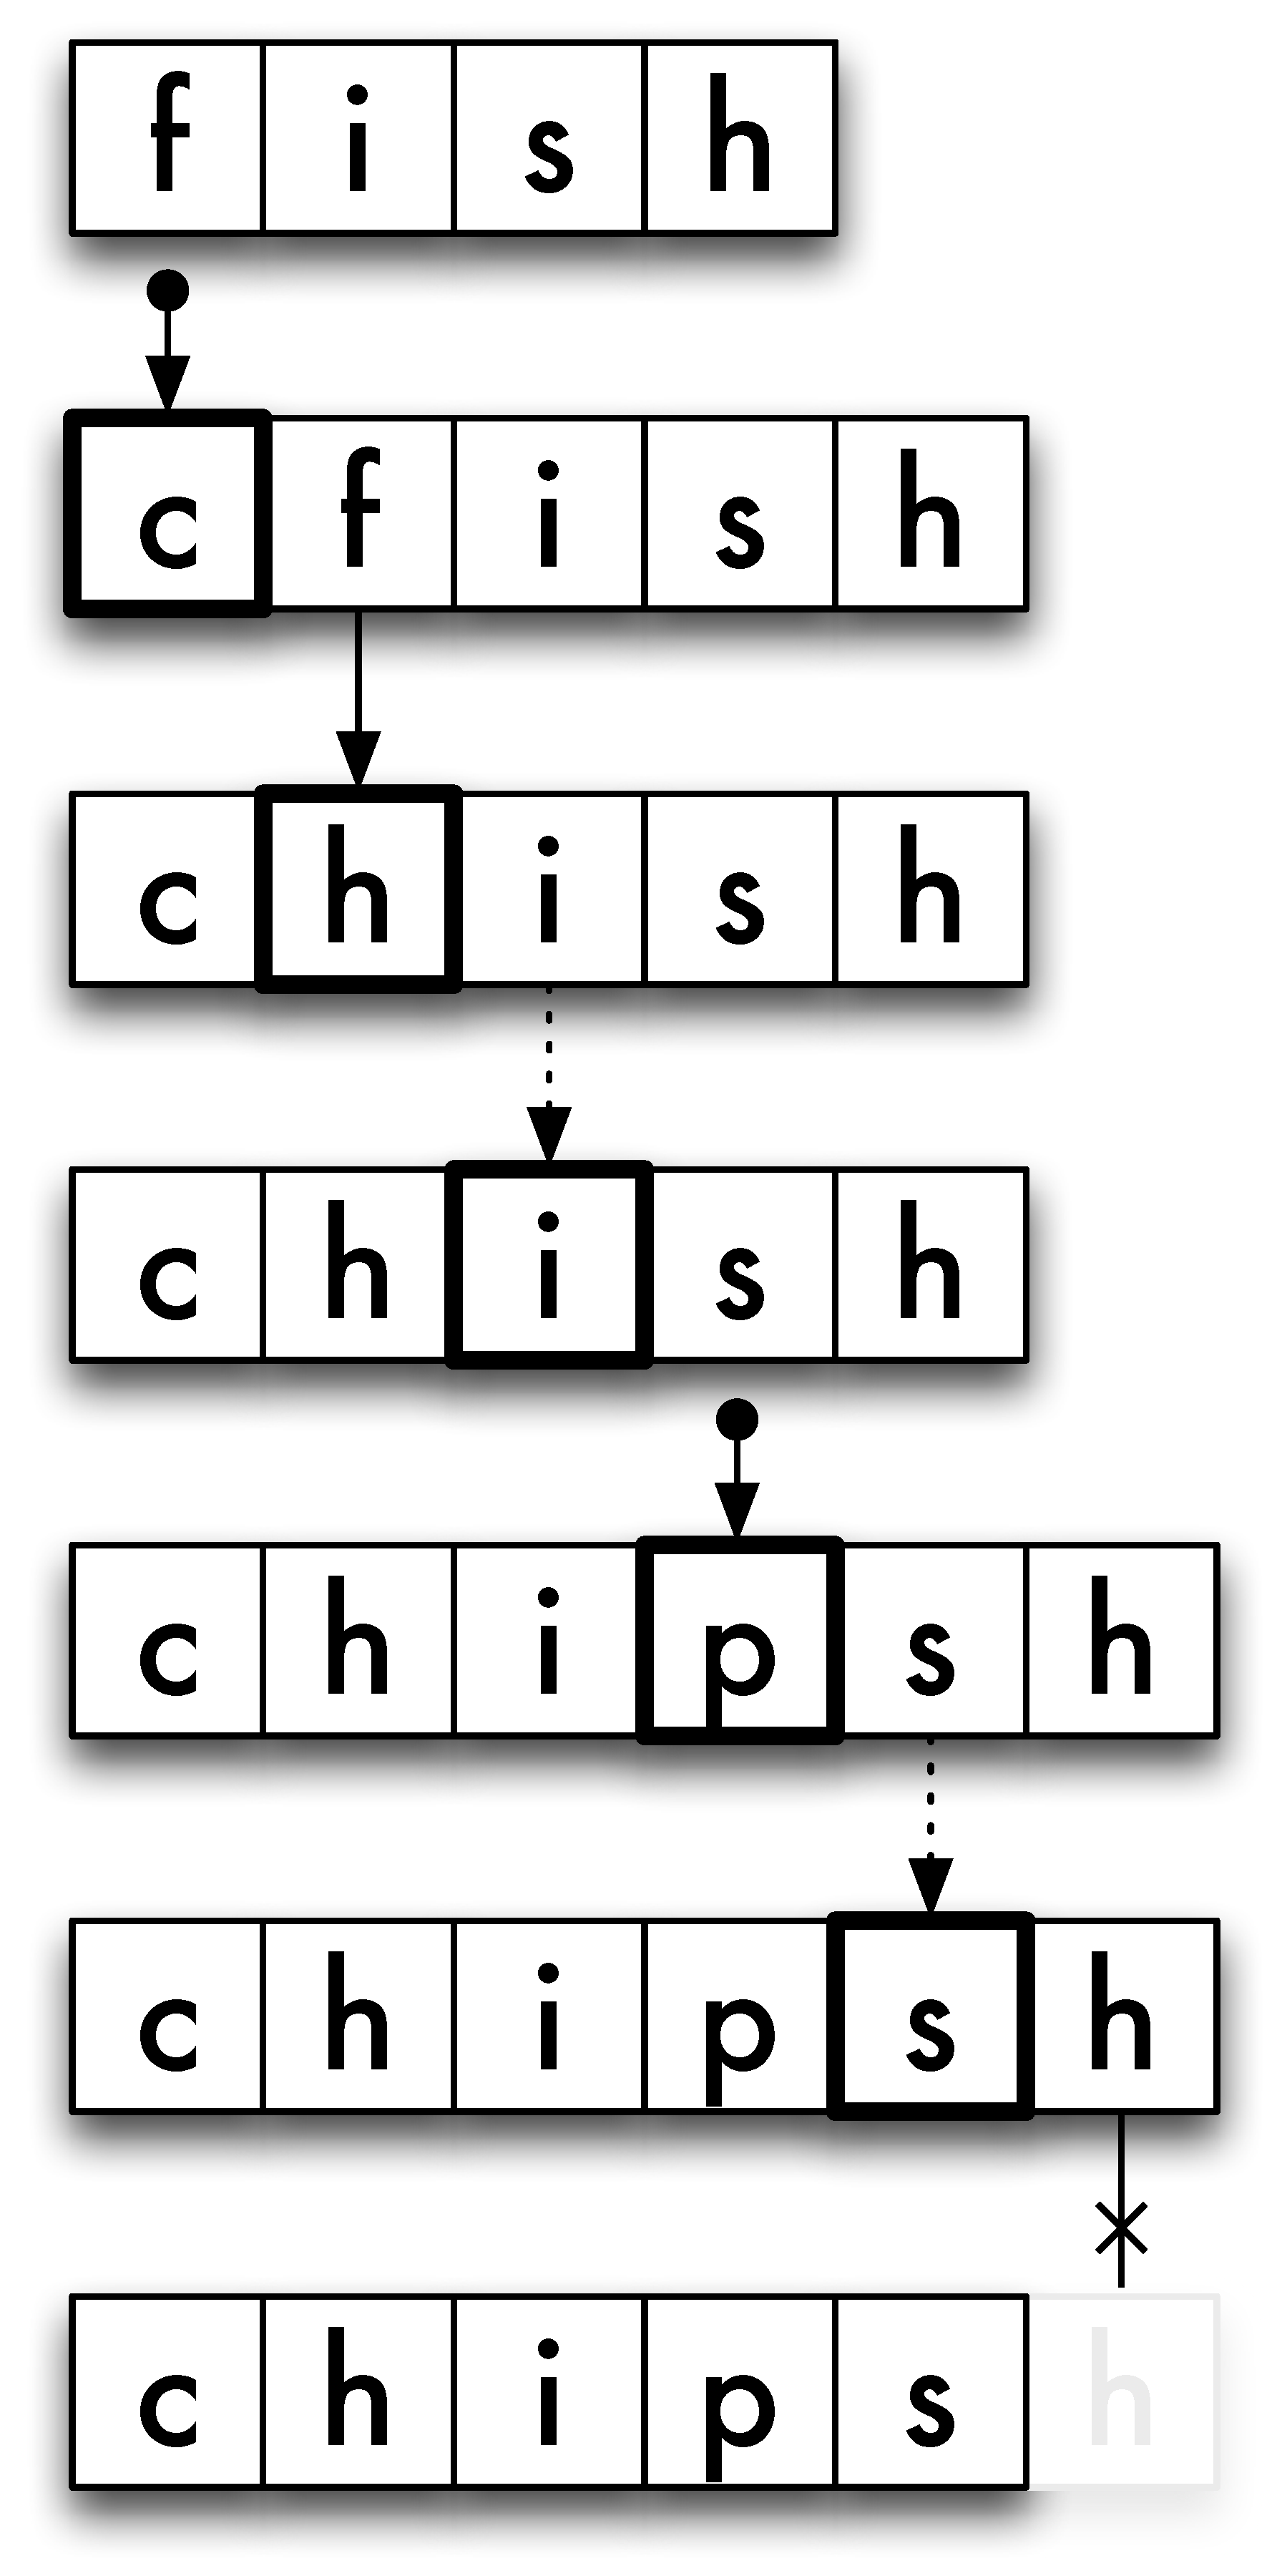
\includegraphics[width=4cm]{Pictures/FishChips.pdf}
\end{wrapfigure}
To turn the string \texttt{"fish"} into \texttt{"chips"}, we could kill the
whole string, then insert the characters one-by-one, at a total cost of six.
An optimal solution will copy as much of the string as possible, and is given
by 
\begin{titemize}
\item inserting the character \texttt{'c'}, 
\item changing \texttt{'f'} to \texttt{'h'},
\item copying \texttt{'i'},
\item inserting \texttt{'p'},
\item copying \texttt{'s'}, and finally
\item deleting the remainder of the string, \texttt{"h"}.
\end{titemize}
In the remainder of this section we design a type to represent the editing
steps, and after looking at another example of data type design, define a
function to give an optimal sequence of editing steps from one string to
another.

The analysis here can also be used to describe the difference between two
lists of arbitrary type. If each item is a line of a file, the behaviour
of the function is similar to the Unix \texttt{diff} utility, which is
used to give the difference between two text files.

\subsection*{Design stages in the edit distance problem}

Now we look at the three stages of algebraic type definition in detail.
\begin{titemize}
\item First we have to identify the {\em types\/} of data involved. In the
example, we have to define
\begin{alltt}
data Edit = ...\minx{Edit}
\end{alltt}
which represents the editing operations.
\item Next, we have to identify the different sorts of data in each of
the types. Each sort of data is given by a \textbf{constructor}\index{constructor}. In the
example, we can change, copy, delete or insert a character and delete (kill)
to the end of the string. Our type definition is therefore
\begin{alltt}
data Edit = Change ... |
            Copy ... |
            Delete ... |
            Insert ... |
            Kill ... 
\end{alltt}
The `\texttt{...}' show that we have not yet said anything about the types of the
constructors. 
\item
Finally, for each of the constructors, we need to decide what its \textbf{components} or arguments are. Some of the constructors -- \texttt{Copy}, 
\texttt{Delete} and \texttt{Kill} -- require no information; the others need to indicate
the new character to be inserted, so
\begin{alltt}
data Edit = Change Char |
            Copy |
            Delete |
            Insert Char |
            Kill  
            deriving (Eq,Show)\minx{deriving}
\end{alltt}
This completes the definition.
\end{titemize}
We now illustrate how other type definitions work in a similar way,
before returning to give a solution to the `edit distance' problem.
\index{edit distance|)}
%\pagebreak

\subsection*{Simulation}
\index{case studies!simulation|see{simulation}}
\index{simulation|(}
\vspace{3pt}

Suppose we want to model, or \textbf{simulate}, how the queues in a bank or Post
Office behave; perhaps we want to decide how many bank clerks need to be
working at particular times of the day. Our system will take as input the
arrivals of customers, and give as output their departures. Each of these can
be modelled using a type.
\vspace{3pt}
\begin{titemize}
\item \texttt{Inmess}\minx{Inmess} is the type of input messages. At a given time, there are
two possibilities:
\vspace{3pt}
\begin{titemize}
\item[--] No-one arrives, represented by the 0-ary constructor \texttt{No};
\item[--] Someone arrives, represented by the constructor \texttt{Yes}. This will
have components giving the arrival time of the customer, and the amount of time
that will
be needed to serve them. 
\end{titemize}
Hence we have
\begin{alltt}
data Inmess = No | Yes Arrival Service

type Arrival = Integer
type Service = Integer
\end{alltt}  
\item Similarly, we have \texttt{Outmess}\minx{Outmess}, the type of output messages. Either
no-one leaves (\texttt{None}), or a person is discharged (\texttt{Discharge}). The
relevant information they carry is the time they have waited, together with
when they arrived and their service time. We therefore define
\begin{alltt}
data Outmess = None | Discharge Arrival Wait Service

type Wait = Integer
\end{alltt}
\end{titemize}
We return to the simulation example in Chapter \ref{adt}.
\index{simulation|)}


\subsection*{Edit distance: solution}
\index{edit distance|(}
\vspace{3pt}

The problem is to find the lowest-cost sequence of edits to take us from one
string to another. We can begin the definition thus:
\begin{alltt}
transform :: String -> String -> [Edit]\minx{transform}

transform [] [] = []
\end{alltt}
To transform the non-empty string \texttt{st} to \texttt{[]}, we simply have to
\texttt{Kill} it, while to transform \texttt{[]} to \texttt{st} we have to 
\texttt{Insert} each of the characters in turn:
\begin{alltt}
transform xs [] = [Kill]
transform [] ys = map Insert ys
\end{alltt}
In the general case, we have a choice: should we first use \texttt{Copy}, 
\texttt{Delete}, \texttt{Insert} or \texttt{Change}? If the first characters of the
strings are equal we should copy; but if not, there is no obvious choice. We
therefore try {\em all\/} possibilities and choose the best of them:
\begin{alltt}
transform (x:xs) (y:ys)
  | x==y        = Copy : transform xs ys
  | otherwise   = best [ Delete   : transform xs (y:ys) ,
                         Insert y : transform (x:xs) ys ,
                         Change y : transform xs ys ]
\end{alltt}
How do we choose the \texttt{best} sequence? We choose the one with the lowest
cost.
\begin{alltt}\minx{best}
best :: [[Edit]] -> [Edit]
best [x]   = x
best (x:xs) 
  | cost x <= cost b    = x
  | otherwise           = b
      where 
      b = best xs
\end{alltt}
The \texttt{cost} is given by charging one for every operation except copy,
which is equivalent to `leave unchanged'.
\begin{alltt}
cost :: [Edit] -> Int\minx{cost}
cost = length . filter (/=Copy)
\end{alltt}
\index{design!and algebraic types|)}
\index{edit distance|)}


\beware{Testing \texttt{transform} using QuickCheck}{\index{QuickCheck!testing edit distance}
We can use to QuickCheck to test two of the fundamental properties of the \texttt{transform} function. 

\medskip
First, it should produce a list whose cost is no bigger than the cost of building up the target string letter by letter, and then killing the original string, a cost of \texttt{length ys + 1}: we can state this as the property
\begin{alltt}
prop\_transformLength :: String -> String -> Property

\ 

prop\_transformLength xs ys =

\ \ \ \ length (xs++ys) <= 15 ==> 

\ \ \ \ \ \ \ \ cost (transform xs ys) <= length ys + 1
\end{alltt}
where we have guarded the test on the overall length of the two lists, for efficiency reasons.

\medskip
Secondly, the sequence of edits given by \texttt{transform xs ys} should indeed take the string \texttt{xs} to \texttt{ys} when it is applied, so
\begin{alltt}
prop\_transform xs ys =

\ \ \ \ length (xs++ys) <= 15 ==> 

\ \ \ \ \ \ \ \ edit (transform xs ys) xs == ys
\end{alltt}
We leave it as an exercise for the reader to define the function 
\begin{alltt}
edit :: [Edit] -> String -> String
\end{alltt}
so that, for instance
\begin{alltt}
edit [Insert 'c',Change 'h',Copy,Insert 'p',Copy,Kill] "fish"

\ \ \ \step{} "chips"
\end{alltt}
}


\begin{exercises}


\item
How would you modify the edit distance program to accommodate a \texttt{Swap}
operation, which can be used to transform \texttt{"abxyz"} to \texttt{"baxyz"} in a
single step?

\item
Write a definition of the \texttt{edit} function described above, which when given a list of edits and a string \texttt{st},
returns the sequence of strings given by applying the edits to \texttt{st} in
sequence.

\item
Can you give other QuickCheck properties that you would expect the edit distance program to have? You could think, for example, about particular sorts of inputs, e.g. where the input is an initial segment of the output.

\item
Give a calculation of \texttt{transform "cat" "am"}. What do you conclude about
the efficiency of the \texttt{transform} function?

\item {[Harder]}
Can you give a more efficient implementation of the function calculating the \texttt{transform}?

\end{exercises}
 
 
\noindent
The remaining questions are designed
to make you think about how data types are designed. These
questions are not intended to have a single `right' answer,
rather you should satisfy yourself that you have adequately
represented the types which appear in your informal picture of
the problem.

\begin{exercises}

\item
It is decided to keep a record of vehicles which will use a particular car
park. Design an algebraic data type to represent them.

\item
If you knew that the records of vehicles were to be used for comparative
tests of fuel efficiency, how would you modify your answer to the last
question?

\item
Discuss the data types you might use in a database of students' marks for
classes and the like. Explain the design of any algebraic data types that
you use.

\item
What data types might be used to represent the objects which can be drawn
using an interactive drawing program? To give yourself more of a challenge, you
might like to think about grouping of objects, multiple copies of objects, and
scaling. 
 
\end{exercises} 
 
 
\section{Algebraic types and type classes}
\label{algClasses}
\index{classes!and algebraic types|(}
\index{design!type classes}
\label{oop}


We have reached a point where it is possible to explore rather more
substantial examples of type classes, first introduced in Chapter \ref{typeClasses}. 

\subsection*{Movable objects}



\begin{figure}[t]
\begin{alltt}
data Vector = Vec Float Float\minx{Vector}

class Movable a where\minx{Movable}
  move      :: Vector -> a -> a
  reflectX  :: a -> a
  reflectY  :: a -> a
  rotate180 :: a -> a
  rotate180 = reflectX . reflectY

data Point = Point Float Float 
             deriving Show

instance Movable Point where\minx{Point}
  move (Vec v1 v2) (Point c1 c2) = Point (c1+v1) (c2+v2)
  reflectX (Point c1 c2)  = Point c1 (-c2)
  reflectY (Point c1 c2)  = Point (-c1) c2
  rotate180 (Point c1 c2) = Point (-c1) (-c2)
\end{alltt}
\caption{Movable objects (1).}
\label{movOb1}
\end{figure}

\begin{figure}[t]
\begin{alltt}
data Figure = Line Point Point |\minx{Figure}
              Circle Point Float 
              deriving Show

instance Movable Figure where
  move v (Line p1 p2) = Line (move v p1) (move v p2)
  move v (Circle p r) = Circle (move v p) r

  reflectX (Line p1 p2) = Line (reflectX p1) (reflectX p2)
  reflectX (Circle p r) = Circle (reflectX p) r

  reflectY (Line p1 p2) = Line (reflectY p1) (reflectY p2)
  reflectY (Circle p r) = Circle (reflectY p) r

instance Movable a => Movable [a] where
  move v   = map (move v)
  reflectX = map reflectX
  reflectY = map reflectY
\end{alltt}
\caption{Movable objects (2).}
\label{movOb2}
\end{figure}



We start by 
building a class of types whose members are geometrical objects in two
dimensions. The operations of the class are those to move the objects in
various different ways.

We now work through the definitions, which are
illustrated in Figures \ref{movOb1} and \ref{movOb2}.
Some moves will be dictated by vectors, so we
first define

\begin{alltt}
data Vector = Vec Float Float
\end{alltt}
The class definition itself is
\begin{alltt}
class Movable a where
  move      :: Vector -> a -> a
  reflectX  :: a -> a
  reflectY  :: a -> a
  rotate180 :: a -> a
  rotate180 = reflectX . reflectY
\end{alltt}
and it shows the ways in which an object can be moved. First
it can be moved by a vector, as in the diagram below.

\medskip
\noindent
\begin{center}
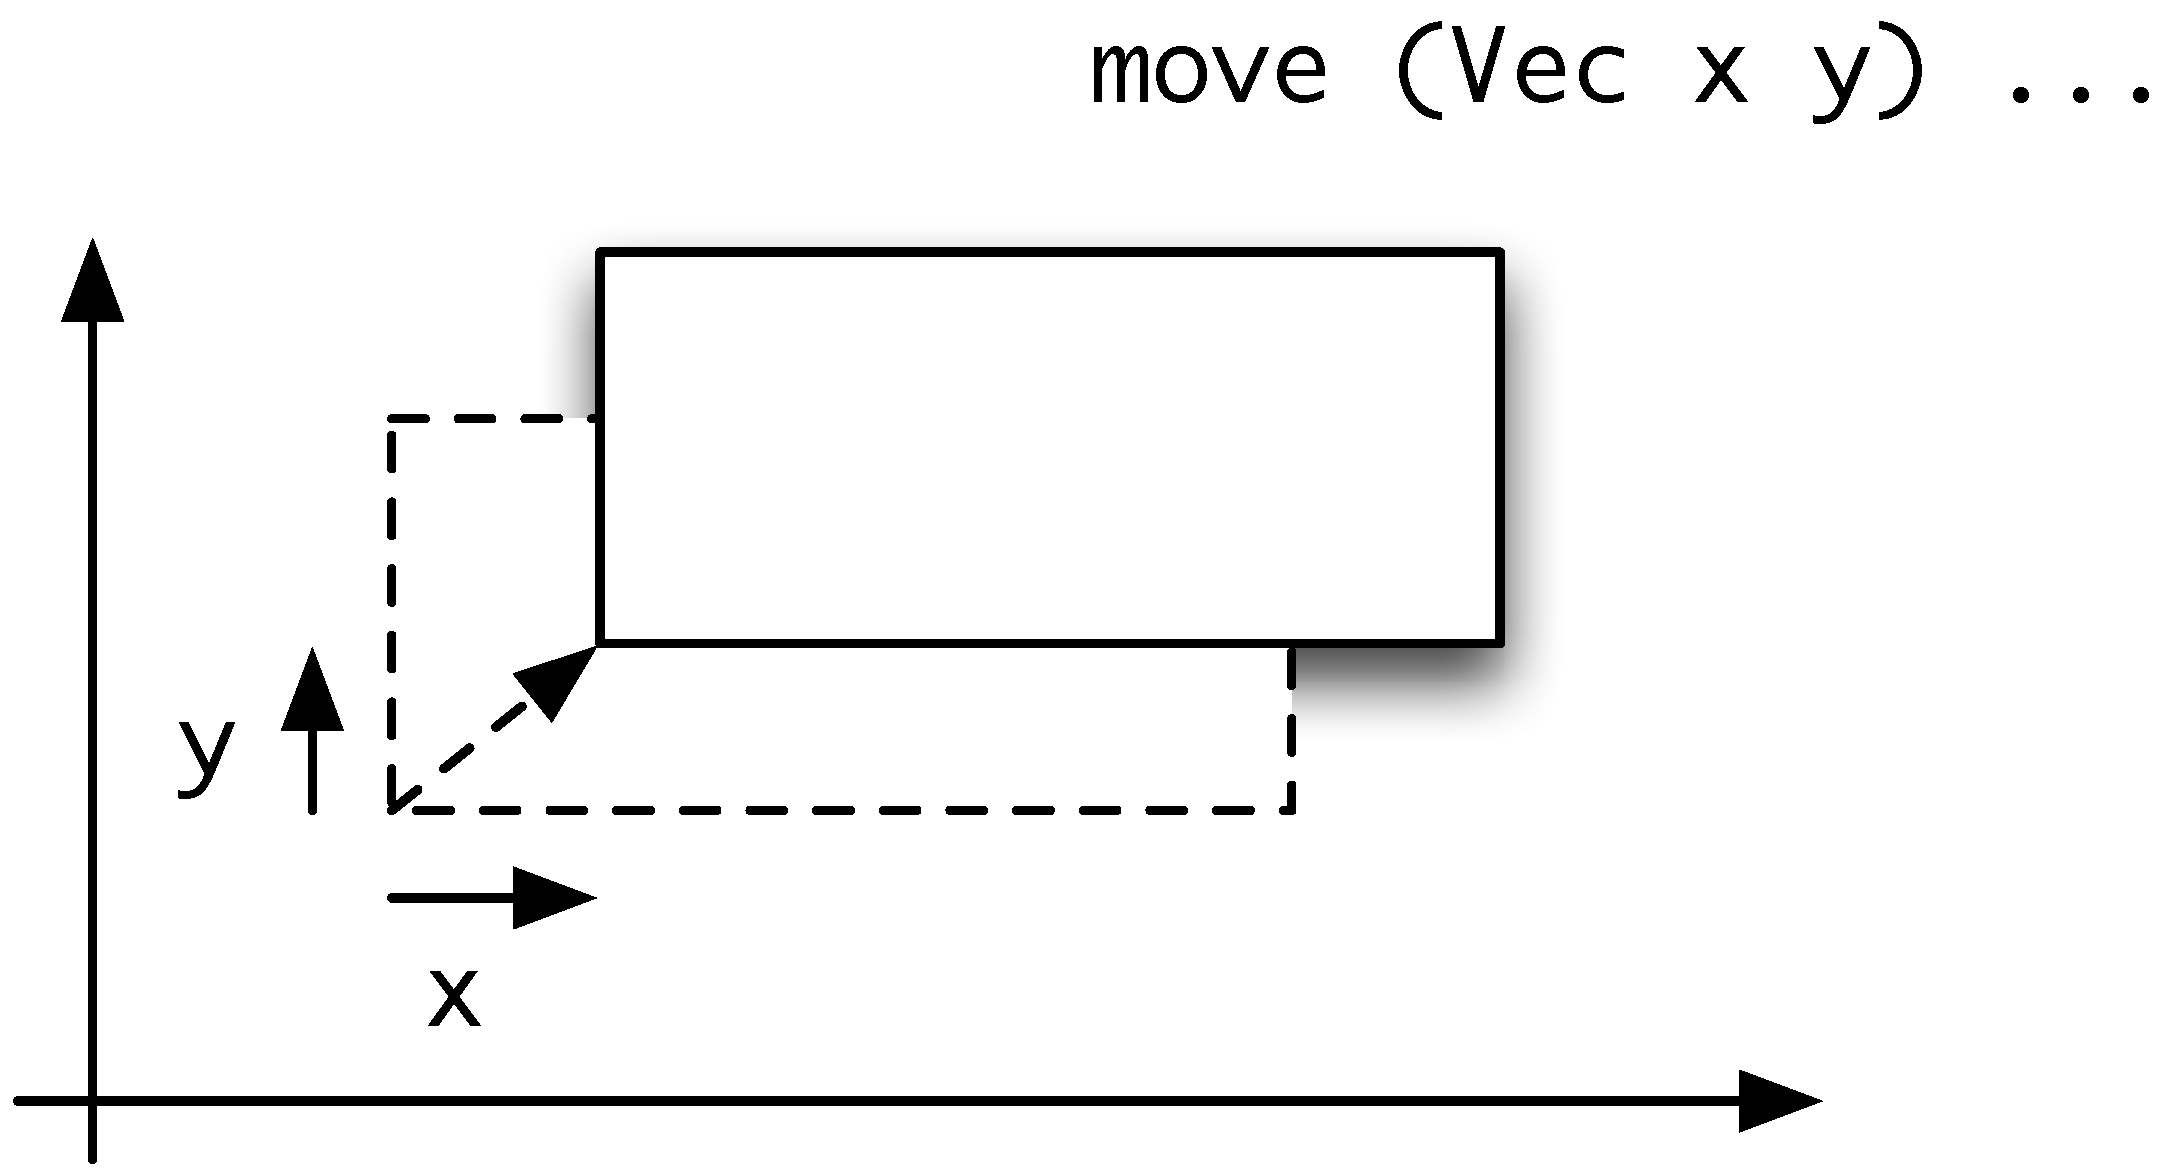
\includegraphics[width=3in]{Pictures/moveVec.pdf}
\end{center}

\begin{figure}[t]
\begin{alltt}
data Name a = Pair a String

exam1 = Pair (Point 0.0 0.0) "Dweezil"

instance Named (Name a) where\hfill(1)
  lookName (Pair obj nm) = nm
  giveName nm (Pair obj _) = (Pair obj nm)

mapName :: (a -> b) -> Name a -> Name b

mapName f (Pair obj nm) = Pair (f obj) nm

instance Movable a => Movable (Name a) where\hfill(2)
  move v   = mapName (move v)
  reflectX = mapName reflectX
  reflectY = mapName reflectY

class (Movable b, Named b) => NamedMovable b\hfill(3)\minx{NamedMovable}

instance Movable a => NamedMovable (Name a)
\end{alltt}
\caption{Named movable objects.}
\label{nMovObj}
\vspace{5pt}
\end{figure}



We can also reflect an object in the x-axis (the horizontal axis) or the y-axis
(the vertical),
or rotate a figure through $180^{\circ}$ around the origin (the point where
the axes meet). The default definition
of \texttt{rotate180} works by reflecting first in the y-axis and then
the x, as we did with the \texttt{Picture} type in Chapter \ref{intro}.


We can now define a hierarchy of movable objects; first we have the 
\texttt{Point},
\begin{alltt}
data Point = Point Float Float
             deriving Show
\end{alltt}
To make \texttt{Point} an instance of \texttt{Movable} we have to give
definitions of \texttt{move}, \texttt{reflectX} and \texttt{reflectY}
over the \texttt{Point} type.
\begin{alltt}
move (Vec v1 v2) (Point c1 c2) = Point (c1+v1) (c2+v2)
\end{alltt}
Here we can see that the move is achieved by adding the components \texttt{v1}
and \texttt{v2} to the coordinates of the point.
Reflection is given by changing the sign of one of the coordinates
\begin{alltt}
reflectX (Point c1 c2) = Point c1 (-c2)
reflectY (Point c1 c2) = Point (-c1) c2
\end{alltt}
For this instance we\index{classes!overriding defaults}
override the default definition of \texttt{rotate180} by changing the sign
of both coordinates. This is a more efficient way of achieving the same
transformation than the default definition.
\begin{alltt}
rotate180 (Point c1 c2) = Point (-c1) (-c2)
\end{alltt}
Using the type of points we can build figures:
\begin{alltt}
data Figure = Line Point Point |
              Circle Point Float
\end{alltt}
and in the instance declaration of \texttt{Movable} for \texttt{Figure} given in Figure
\ref{movOb2} we use the corresponding
operations on \texttt{Point}; for example,
\begin{alltt}
move v (Line p1 p2) = Line (move v p1) (move v p2)
move v (Circle p r) = Circle (move v p) r       
\end{alltt}
This same approach works again when we consider a list of movable objects:
\begin{alltt}
instance Movable a => Movable [a] where
  move v   = map (move v)
  reflectX = map reflectX
\end{alltt}
and so on. Using overloading in this way has a number of advantages.
\begin{titemize}
\item The code is much easier to read: at each point we write \texttt{move},
rather than \texttt{movePoint}, and so on.
\item We can reuse definitions; the instance declaration for 
\texttt{Movable [a]} makes lists of any sort of movable object movable themselves.
This includes lists of
points and lists of figures. Without overloading we would not be able to
achieve this.
\end{titemize}\index{overloading!advantages of}

\subsection*{Named objects}

Many forms of data contain some sort of name, a \texttt{String} which identifies
the object in question. What do we expect to be able to do with a value of
such a type?
\begin{itemize}
\item We should be able to identify the name of a value, and
\item we ought to be able to give a new name to a value.
\end{itemize}
These operations are embodied in the \texttt{Named} class:
\begin{alltt}
class Named a where\minx{Named}
  lookName :: a -> String
  giveName :: String -> a -> a
\end{alltt}
and an example of \texttt{Named} types is given by
\begin{alltt}
data Name a = Pair a String\minx{Name}
\end{alltt}
the one-constructor type whose two components are of type \texttt{a} and 
\texttt{String}. The \texttt{instance} declaration for this type is
\begin{alltt}
instance Named (Name a) where\hfill(1)
  lookName (Pair obj nm) = nm
  giveName nm (Pair obj _) = (Pair obj nm)
\end{alltt}

\subsection*{Putting together classes}
\index{classes!putting together}

An important aspect of object-oriented software development is the way in
which one class can be built upon another, reusing the operations of the
original class on the subclass. In this section we explore how to combine the
\texttt{Movable} and \texttt{Named} classes, to give objects which are both movable
and named. The section is
rather more advanced, and
can be omitted on first reading.


Suppose we are to add names to our movable objects -- how might this be done?
We examine one approach in the text, and another in the exercises.

Our approach is to build the type \texttt{Name a} where elements of type \texttt{a}
are movable, that is \texttt{Movable a} holds. We then
want to establish that the type \texttt{Name a} is in both the classes 
\texttt{Movable} and \texttt{Named}. We have shown the latter for {\em any\/} type 
\texttt{a} already in \texttt{(1)} above, so we concentrate on the former.


The crucial insight is that the naming is independent of the named type; any
operation on the type can be \textbf{lifted} to work over named types thus:
\begin{alltt}\minx{mapName}
mapName :: (a -> b) -> Name a -> Name b

mapName f (Pair obj nm) = Pair (f obj) nm
\end{alltt}
We can then argue that all the operations of the \texttt{Movable} class can be
lifted.
\begin{alltt}
instance Movable a => Movable (Name a) where\hfill(2)
  move v   = mapName (move v)
  reflectX = mapName reflectX
  reflectY = mapName reflectY
\end{alltt}
Now we already know that \texttt{Named (Name a)} by \texttt{(1)} above, so
if we define a class combining these attributes
\begin{alltt}
class (Movable b, Named b) => NamedMovable b\hfill(3)
\end{alltt}
we can declare the instance
\begin{alltt}
instance Movable a => NamedMovable (Name a)
\end{alltt}
This last instance is established by showing that the two constraints of
\texttt{(3)} hold when \texttt{b} is replaced by \texttt{Name a},
but this is exactly what \texttt{(1)} and \texttt{(2)} say given the constraint 
\texttt{Movable a}. 


This completes the demonstration that \texttt{NamedMovable (Name a)}
holds when we know that \texttt{Movable a}. It is worth realising that this demonstration is
produced automatically by the Haskell system -- we only need to type what is
seen in Figure \ref{nMovObj}.

This section has begun to illustrate how classes can be used in the software
development process. In particular we have shown how our movable objects can
be named in a way which allows reuse of all the code to move the objects.
\index{reuse}

\index{classes!and algebraic types|)}


\vspace{8pt}

\begin{exercises}
\vspace{3pt}

\item
A different way of combining the classes \texttt{Named} and \texttt{Movable} is to
establish the instance
\begin{alltt}
instance (Movable b,Named c) => NamedMovable (b,c)
\end{alltt}
This is done by giving the instances
\begin{alltt}
instance Movable b => Movable (b,c) where ....
instance Named c   => Named (b,c) where ....
\end{alltt}
Complete these instance declarations.

\item 
Show that the method of the previous question can be used to combine
instances of {\em any\/} two classes.

\item
The example in the final part of this section shows how we can combine an
arbitrary instance of the \texttt{Movable} class, \texttt{a},
with a {\em particular\/}
instance of the \texttt{Named} class, \texttt{String}. Show how it can be used to
combine an arbitrary instance of one class with a particular instance of
another for {\em any\/} two classes whatever.

\item
Extend the collection of operations for moving objects to include scaling and
rotation by an arbitrary angle. This can be done by re-defining \texttt{Movable}
or by defining a class \texttt{MovablePlus} over the class \texttt{Movable}. Which
approach is preferable? Explain your answer.

\item
Design a collection of classes to model bank accounts. These have different
forms: current, deposit and so on, as well as different levels of
functionality. Can you reuse the \texttt{Named} class here?
\end{exercises}

\section{Reasoning about algebraic types}
\index{proof!algebraic types}
\index{algebraic type!proofs}
%\label{algProofs}
\label{proofAlgTypes}

Verification for algebraic types follows the example of lists, as first
discussed in Chapter \ref{reasoningProgs}. The general pattern of structural
induction over an algebraic type states that the result has to be proved for
each constructor; when a constructor is recursive, we are allowed to use the
corresponding induction hypotheses in making the proof. We first give some
representative examples in this section, and conclude with a rather more
sophisticated proof.

\subsection*{Trees}
\minx{Tree}

Structural induction over the type \texttt{Tree}
of trees is stated as follows.
\subsubsection*{Structural induction over trees} 
\index{structural induction!trees}

To prove the property \texttt{P(tr)} for all finite \texttt{tr} of type 
\texttt{Tree t} we have to do two things.

\medskip
\noindent
\begin{mytable}
\bf \texttt{Nil} case & Prove \texttt{P(Nil)}. \\
\bf \texttt{Node} case & Prove \texttt{P(Node x tr1 tr2)} for all
\texttt{x} of
type \texttt{t}\\
& assuming that \texttt{P(tr1)} and 
\texttt{P(tr2)} hold already.
\end{mytable}

\medskip
\noindent
The advice of Chapter \ref{reasoningProgs} about finding proofs can easily be carried over to
the situation here. 
Now we give a representative
example of a proof. We aim to prove for all finite trees \texttt{tr} that
\begin{alltt}\index{map@\texttt{map}}\minx{collapse}\minx{mapTree}
map f (collapse tr) = collapse (mapTree f tr)\hfill(map-collapse)
\end{alltt}
which states that if we map a function over a tree, and then collapse the
result we get the same result as collapsing before mapping over the list.
The functions we use are defined as follows
\begin{alltt}
map f []     = [] \hfill (map.1)\index{map@\texttt{map}}
map f (x:xs) = f x : map f xs \hfill (map.2)

mapTree f Nil = Nil\hfill (mapTree.1)\minx{mapTree}
mapTree f (Node x t1 t2)
  = Node (f x) (mapTree f t1) (mapTree f t2) \hfill (mapTree.2)

collapse Nil = []\hfill (collapse.1)\minx{collapse}
collapse (Node x t1 t2)
  = collapse t1 ++ [x] ++ collapse t2\hfill (collapse.2)
\end{alltt}

\subparagraph{Base} In the \texttt{Nil} case, we simplify each side, giving
\begin{alltt}
map f (collapse Nil)
  = map f [] \hfill {\rm by} (collapse.1)
  = [] \hfill  {\rm by} (map.1)

collapse (mapTree f Nil)
  = collapse Nil \hfill {\rm by} (mapTree.1)
  = [] \hfill {\rm by} (collapse.1)
\end{alltt}
This shows that the base case holds.

\subparagraph{Induction} 
In the \texttt{Node} case, we have to prove:
\begin{alltt}
map f (collapse (Node x tr1 tr2)) 
  = collapse (mapTree f (Node x tr1 tr2))\hfill(ind)
\end{alltt}
assuming the two induction hypotheses:
\begin{alltt}
map f (collapse tr1) = collapse (mapTree f tr1) \hfill (hyp.1)
map f (collapse tr2) = collapse (mapTree f tr2)\hfill (hyp.2)
\end{alltt}
Looking at \texttt{(ind)}, we can simplify the left-hand side thus
\begin{alltt}
map f (collapse (Node x tr1 tr2))
  = map f (collapse tr1 ++ [x] ++ collapse tr2)\hfill{\rm by} (collapse.2)
  = map f (collapse tr1) ++ [f x] ++ map f (collapse tr2)
       \hfill{\rm by} (map++)
  = collapse (mapTree f tr1) ++ [f x] ++ 
    collapse (mapTree f tr2)\hfill{\rm by} (hyp1,hyp2) 
\end{alltt}
The final step is given by the two induction hypotheses, that the result
holds for the two subtrees \texttt{tr1} and \texttt{tr2}. The result \texttt{(map++)} is the
theorem
\begin{alltt}
map g (ys++zs) = map g ys ++ map g zs \hfill (map++)
\end{alltt}
discussed in Chapter \ref{gen2}. Examining the right-hand side now, we have
\begin{alltt}
collapse (mapTree f (Node x tr1 tr2))
  = collapse (Node (f x) (mapTree f tr1) 
                         (mapTree f tr2))\hfill{\rm by} (mapTree.2)
  = collapse (mapTree f tr1) ++ [f x] ++ 
    collapse (mapTree f tr2)\hfill{\rm by} (collapse.2)
\end{alltt}
and this finishes the proof in the \texttt{Node} case. As this is the
second
of the two cases, the proof is complete. 
\blackbox

\subsection*{The \texttt{Maybe} type}
\index{error handling!error type}
\minx{Maybe}

Structural induction for the type \texttt{Maybe t} becomes proof by cases --
because the type is not recursive, in none of the cases is there an appeal to
an induction hypothesis. The rule is

\subsubsection*{Structural induction over the \texttt{Maybe} type} 
\index{structural induction!\texttt{Maybe} type}

To prove the property \texttt{P(x)} for all defined\footnote{When the type is
not recursive, the induction principle gives a proof for all defined objects.
An object of this type is defined if it is \texttt{Nothing}, or \texttt{Just y} for a
defined \texttt{y}.}  \texttt{x} of type \texttt{Maybe t} we have to do two things:

\medskip
\noindent
\begin{mytable}
\bf \texttt{Nothing} case & Prove \texttt{P(Nothing)}. \\
\bf \texttt{Just} case & Prove \texttt{P(Just y)} for all defined \texttt{y} of type \texttt{t}.
\end{mytable}

\medskip
\noindent
Our example proof is that, for all defined values \texttt{x} of type 
\texttt{Maybe Int},
\begin{alltt}
maybe 2 abs x \(\geq\) 0\minx{maybe}
\end{alltt}

\startpr\ The proof has two cases. In the first \texttt{x} is replaced by 
\texttt{Nothing}:
\begin{alltt}
maybe 2 abs Nothing
  = 2 \(\geq\) 0
\end{alltt}
In the second, \texttt{x} is replaced by \texttt{Just y} for a defined \texttt{y}.
\begin{alltt}
maybe 2 abs (Just y)
  = abs y \(\geq\) 0
\end{alltt}
In both cases the result holds, and so the result is valid in general.
\blackbox

\subsection*{Other forms of proof}
\index{proof!non-primitive recursive}

We have seen that not all functions are defined by primitive recursion. The
example we saw in Section \ref{recTypes} was of the function \texttt{assoc},
which is used to rearrange arithmetic expressions represented by the type \texttt{Expr}. 
Recall that
\begin{alltt}
assoc (Add (Add e1 e2) e3)\minx{assoc}
  = assoc (Add e1 (Add e2 e3)) \hfill (assoc.1)
assoc (Add e1 e2) = Add (assoc e1) (assoc e2)\hfill (assoc.2)
assoc (Sub e1 e2) = Sub (assoc e1) (assoc e2)\hfill (assoc.3)
assoc (Lit n)     = Lit n\hfill (assoc.4)
\end{alltt}
with \texttt{(assoc.1)} being the non-primitive recursive case. We would like to
prove that the rearrangement does not affect the value of the expression:
\begin{alltt}\minx{eval}
eval (assoc ex) = eval ex \hfill (eval-assoc)
\end{alltt}
for all finite expressions \texttt{ex}. The induction principle for the \texttt{Expr}
\index{structural induction!expression type}
type has three cases.

\medskip
\noindent
\begin{mytable}
\bf \texttt{Lit} case & Prove \texttt{P(Lit n)}. \\
\bf \texttt{Add} case & Prove \texttt{P(Add e1 e2)}, assuming \texttt{P(e1)} and 
\texttt{P(e2)} \\
\bf \texttt{Sub} case & Prove \texttt{P(Sub e1 e2)}, assuming \texttt{P(e1)} and 
\texttt{P(e2)}
\end{mytable}

\medskip
\noindent
To prove \texttt{(eval-assoc)} for all finite expressions, we have the three cases given
above. The \texttt{Lit} and \texttt{Sub} cases are given, respectively, by 
\texttt{(assoc.4)} and \texttt{(assoc.3)}, but the \texttt{Add} case is more subtle. 
For this we will
prove
\begin{alltt}
eval (assoc (Add e1 e2)) = eval (Add e1 e2) \hfill (eval-Add)
\end{alltt}
by induction on the number of \texttt{Add}s which are left-nested at the top
level of the expression \texttt{e1} -- recall that it was by counting these
and noting that \texttt{assoc} preserves the total number of \texttt{Adds} overall
that we proved the function would always terminate. Now, if there are no 
\texttt{Add}s at the top-level of \texttt{e1}, the equation \texttt{(assoc.2)} gives \texttt{(eval-Add)}.
Otherwise we rearrange thus:
\begin{alltt}
eval (assoc (Add (Add f1 f2) e2))) 
= eval (assoc (Add f1 (Add f2 e2)))\hfill {\rm by} (assoc.1) 
\end{alltt}
and since \texttt{f1} contains fewer \texttt{Add}s at top level, 
\begin{alltt}
= eval (Add f1 (Add f2 e2))
= eval (Add (Add f1 f2) e2) \hfill {\rm by associativity of} +
\end{alltt}
which gives the induction step, and therefore completes the proof. 
\blackbox

This result shows that verification is possible for functions defined in a
more general way than primitive recursion.

\begin{figure}[t]\index{QuickCheck!properties of trees}
\beware{Checking properties in QuickCheck}{
Many of these properties can be checked in QuickCheck; we can define properties like this:
\begin{alltt}
prop\_assoc :: Expr -> Bool

prop\_assoc expr = 

\ \ \ \ eval expr == eval (assoc expr)

\ 

prop\_depth :: NTree -> Bool

prop\_depth t =

\ \ \ \ size t < 2\^{}(depth t)

\ 
    
prop\_collapse :: Eq b => (a -> b) -> Tree a -> Bool

prop\_collapse f =

\ \ \ \ \bs{t} -> map f (collapse t) == collapse (mapTree f t)
\end{alltt}
To be checkable, we need to be able to generate random values of the types \texttt{Expr}, \texttt{NTree} and \texttt{Tree a} (for types \texttt{a} for which random values can be generated). We have done this in the module available online, and we will explain the code in more detail in Chapter \ref{dsls}.
}
\end{figure}



\begin{exercises}

\item
Prove that the function \texttt{weather}\minx{weather} from Section \ref{introAlg} has the same
behaviour as  
\begin{alltt}
newWeather = makeHot . isSummer
\end{alltt}
when
\begin{alltt}
makeHot True  = Hot
makeHot False = Cold
isSummer = (==Summer)
\end{alltt}
where recall that \texttt{(==Summer)} is an operator section whose effect is to
test whether its argument is equal to \texttt{Summer}.

\item
Is it the case that the \texttt{area} of each \texttt{Shape} from Section
\ref{introAlg} is non-negative? If so, give a proof; if not, give an example
which shows that it is not the case.

\item
If we define the \texttt{size} of an \texttt{NTree} thus
\begin{alltt}
size NilT           = 0
size (Node x t1 t2) = 1 + size t1 + size t2
\end{alltt}
then prove that for all finite \texttt{nTree}s, \texttt{tr},
\begin{alltt}
size tr \(<\) \(\mbox{\texttt{2}}^{\mbox{\texttt{(depth tr)}}}\)
\end{alltt}

\item
Show for all finite \texttt{NTree}s \texttt{tr} that
\begin{alltt}
occurs tr x = length (filter (==x) (collapse tr))
\end{alltt}

\medskip
\noindent
The next two exercises refer back to the exercises of Section \ref{polyAlg}.

\item
Prove that the function \texttt{twist} has the property that
\begin{alltt}
twist . twist = id
\end{alltt}

\item
Explain the principle of structural induction for the type \texttt{GTree}.
Formulate and prove the equivalent of the theorem relating \texttt{map}, 
\texttt{mapTree} and \texttt{collapse} for this type of trees.
\end{exercises}
\begin{summary}
Algebraic types sharpen our ability to model types in our programs: we have
seen in this chapter how simple, finite types like \texttt{Temp} can be defined,
as well as the more complex \texttt{Either} and recursive types. Many of these
recursive types are varieties of tree\index{tree}: we looked at numerical trees; elements
of the type \texttt{Expr} can also be thought of as trees representing the
underlying structure of arithmetical 
expressions.

The type of lists gives a guiding example for various aspects of algebraic
types.
\begin{titemize}
\item The definition of the type is
recursive and polymorphic, and many polymorphic higher-order
functions can be defined over lists -- this carries over to the various types
of tree and the error type, \texttt{Maybe}, for example.
\item There is a simple
principle for reasoning over lists, structural induction, which is the model
for structural induction over algebraic types.
\end{titemize}
The chapter also gives guidelines for defining algebraic types. The definition
can be given in three parts: first the type name is identified, then the
constructors are named, and finally their component types are specified. As
in other aspects of program development, this separation of concerns assists
the system developer to produce simple and correct solutions.

Having introduced algebraic data types we are able to give more substantial
examples of classes and their instances. We can see that the overloading that
classes bring makes code both easier to read and more amenable to reuse; we can see in
particular how software can be extended in a way that requires little
modification to the code.

In the chapters to come, algebraic types will be an integral part of the
systems we develop, and indeed in the next case study we exhibit various
aspects of these types. We shall also explore a different approach to types:
abstract data types, and see how this approach complements and contrasts with
the use of algebraic data types.

\index{algebraic type|)}

\end{summary}



%\end{document}

%\documentclass{book}\usepackage{sjtfonts}\usepackage{includegraphics}\usepackage{alltt}\usepackage{latexsym}
%\usepackage{array}
%\begin{document}\input{defs0}%		miradefs.tex 		    June 1994

% opening and closing a quoted Miranda section

\newcommand{\mira}{\noindent\hrulefill\nopagebreak\so}
\newcommand{\arim}{\nopagebreak\st\hrulefill\\}

% backslash in the Miranda environment
% Only feasible approach is to use \verb+\+
% in line!

%\newcommand{\bs}{$\mi\backslash\!\!$}
%\newcommand{\lbs}{\mbox{\verb+\+}}

% ignoring part of the input

\newcommand{\ignore}[1]{}

% a blank line in a Miranda section

\newcommand{\bl}{\mbox{\ }}

% Signalling a diffculty.

\definecolor{light-gray}{gray}{0.95}

\newcommand{\beware}[2]
 {\medskip\noindent\colorbox{light-gray}{\parbox{\textwidth}
 {\mbox{\large\textbf{#1}} \medskip\noindent\\ #2}\medskip\noindent}}

% Subscripting in Miranda text
\newcommand{\subscr}[2]{\mbox{${\mbox{\texttt{#1}}}_{\mbox{\texttt{#2}}}$}}

%\newcommand{\subscr}[2]{\mbox{${\mbox{\mi #1}}_{\mbox{\smtt #2}}$}}
\newcommand{\aone}{\subscr{a}{1}}
\newcommand{\atwo}{\subscr{a}{2}}
\newcommand{\ak}{\subscr{a}{k}}

\newcommand{\aoneone}{\subscr{a}{1,1}}

\newcommand{\eone}{\subscr{e}{1}}
\newcommand{\etwo}{\subscr{e}{2}}
\newcommand{\ei}{\subscr{e}{i}}
\newcommand{\er}{\subscr{e}{r}}

\newcommand{\fone}{\subscr{f}{1}}
\newcommand{\fl}{\subscr{f}{l}}

\newcommand{\gone}{\subscr{g}{1}}
\newcommand{\gtwo}{\subscr{g}{2}}
\newcommand{\gi}{\subscr{g}{i}}
\newcommand{\gr}{\subscr{g}{r}}

\newcommand{\hone}{\subscr{h}{1}}
\newcommand{\hl}{\subscr{h}{l}}

\newcommand{\pone}{\subscr{p}{1}}
\newcommand{\ptwo}{\subscr{p}{2}}
\newcommand{\pk}{\subscr{p}{k}}

\newcommand{\qone}{\subscr{q}{1}}
\newcommand{\qtwo}{\subscr{q}{2}}
\newcommand{\qk}{\subscr{q}{k}}

\newcommand{\rone}{\subscr{r}{1}}
\newcommand{\rtwo}{\subscr{r}{2}}

\newcommand{\tone}{\subscr{t}{1}}
\newcommand{\ttwo}{\subscr{t}{2}}
\newcommand{\tn}{\subscr{t}{n}}

\newcommand{\vone}{\subscr{v}{1}}
\newcommand{\vtwo}{\subscr{v}{2}}
\newcommand{\vn}{\subscr{v}{n}}

% for regular expressions

\newcommand{\stone}{\subscr{st}{1}}
\newcommand{\sttwo}{\subscr{st}{2}}
\newcommand{\stn}{\subscr{st}{n}}
\newcommand{\rthree}{\subscr{r}{3}}

\newcommand{\eps}{$\varepsilon$}
\newcommand{\trans}[1]{\stackrel{\mbox{\tt #1}}{\longrightarrow}}



% superscript in Miranda text

\newcommand{\superscr}[2]{\mbox{${\mbox{\mi #1}}^{\mbox{\smtt #2}}$}}

% Not equals in Miranda text

\newcommand{\noteq}{\makebox[0pt][l]{=}/}
\newcommand{\overslash}{\makebox[0pt][l]{/}}

% Definitions in complexity chapter

\newfont{\oldSym}{cmsy10}
\newcommand{\Th}{\boldmath$\oldSym\Theta$}
\newcommand{\pow}[1]{\^{}#1}
\newcommand{\leqq}{$\leq$}
\newcommand{\geqq}{$\geq$}
\newcommand{\lll}{$\ll$}
\newcommand{\eqq}{$\equiv$}
\newcommand{\ltwo}{\subscr{log}{2}}

% Indexing

\newcommand{\minx}[1]{\index{#1@{\ttfamily{}#1}}}
\setcounter{chapter}{14}\setcounter{page}{269}

\chapter{Case study: Huffman codes}
\chapstart
\label{codes}
\index{Huffman codes|(}
\index{case studies!Huffman codes|see{Huffman codes}}

We use the case study in this chapter as a vehicle to illustrate many of the
features of the previous chapters -- polymorphism, algebraic types and
program design -- and to illustrate the module system of Haskell,
which is discussed first.


\section{Modules in Haskell}
\index{modules|(}

As we first saw in Section \ref{introModules}, a module
consists of a number of definitions of types, functions and so on, with a
clearly defined \emph{interface} stating what the module \texttt{exports} to
other modules which use or \texttt{import} it. We also saw in Section \ref{HaskellLibs} that module names can be composite, as in \texttt{Data.Bits}, taking the form of hierarchical names.

\medskip
\noindent
Using modules to structure a large program has a number of advantages.
\begin{titemize}
\item Parts of the system can be built separately from each other. Suppose we
want to monitor traffic on a network: one module might produce the statistics,
while another displays them in a suitable form.
If we agree which statistics are to
be presented (their type etc.), that is we agree the interface, then
development of the two parts of the system can go on independently.
\item Parts of a system can be compiled separately; this is a great advantage
for a system of any complexity.
\item Libraries of components can be reused, by importing the appropriate
modules containing them.
\end{titemize}
In the definition of Haskell 2010, there is no identification
between modules and files. Nonetheless, we
choose here to write one module per file, and indeed this is required by GHC.

Now we look at the details of Haskell modules, before giving our case study which
exhibits the system in action.

\subsection*{Module headers}

Each module is named, so an example named \texttt{Ant} might be
\begin{alltt}
module Ant where\minx{module}\minx{Ant}

data Ants  = ...
anteater x = ...
\end{alltt}
Note that the definitions all begin in the column under the keyword
\texttt{module}; it is safest to make this the leftmost column of the
file.


We also assume that a module \texttt{Foo} will live in the file \texttt{Foo.hs}; GHC allows module and file names to be different, but we recommend that you keep them the same. \index{conventions!module file names}

\subsection*{Importing a module}

The basic operation on modules is to \texttt{import} one into another, so in
defining \texttt{Bee} we might say
\begin{alltt}
module Bee where\minx{Bee}

import Ant\minx{import}

beeKeeper = ...
\end{alltt}
This means that the \textbf{visible} definitions from \texttt{Ant}
can be used in 
\texttt{Bee}. By default the visible definitions in\index{visibility of
definitions}\index{definition!visibility of}
a module are those which appear in the module itself. If we define
\begin{alltt}
module Cow where\minx{Cow}

import Bee
\end{alltt}
the definitions of \texttt{Ants} and \texttt{anteater} will not be visible in 
\texttt{Cow}. They can be made visible either by importing \texttt{Ant} explicitly,
or by using the export controls
discussed below to modify exactly what is exported from \texttt{Bee}.


\subsection*{Export controls}
\index{export}

As we explained when \texttt{import} was introduced,
the default is that all top-level definitions of a
module are exported. 
\begin{titemize}
\item This may be too much: we might wish not to export some
auxiliary functions, such as the \texttt{shunt} function below
\begin{alltt}
reverse :: [a] -> [a]
reverse = shunt []

shunt :: [a] -> [a] -> [a]
shunt ys []     = ys
shunt ys (x:xs) = shunt (x:ys) xs
\end{alltt}
since its only role is in defining the \texttt{reverse} function.
\item On the other hand, it might be too little: we perhaps want
to export some of the definitions we imported from other modules. The modules
\texttt{Ant}, \texttt{Bee} and \texttt{Cow} above provide an example of this.
\end{titemize}
We can control what is exported by following the name of the module with a
list of what is to be exported. For instance, we say in the case of \texttt{Bee}
\begin{alltt}
module Bee ( beeKeeper, Ants(..), anteater ) where ...\minx{module}\index{modules!export list}
\end{alltt}
The list contains names of defined objects, such as \texttt{beeKeeper}, and also
\texttt{data} types like \texttt{Ants}.
In the latter case we follow the type name with \texttt{(..)} to indicate
that the constructors of the type are exported with the type
itself; if this is omitted, then the type acts like an \textbf{abstract
data type},\index{abstract data type} which we investigate further in the next chapter. The
\texttt{(..)} is\minx{(..)}
not necessary for a \texttt{type} definition.

Such a list works on a definition-by-definition basis; we can also state that
all the definitions in a module are to be exported, as in
\begin{alltt}
module Bee ( beeKeeper, module Ant ) where ...
\end{alltt}
or equivalently
\begin{alltt}
module Bee ( module Bee , module Ant ) where ...
\end{alltt}
where preceding the name of a module by the keyword \texttt{module} 
is shorthand for
all the names defined within the module. The simple header
\begin{alltt}
module Fish where
\end{alltt}
is therefore equivalent to 
\begin{alltt}
module Fish ( module Fish ) where
\end{alltt}


\beware{The \texttt{Main} module}{
Each system of modules should contain a top-level
module called \texttt{Main}, which gives a
definition to the name \texttt{main}. In a compiled system, this is
the\minx{Main}\minx{main}
expression which is evaluated when the compiled code is run. In an
interpreter like GHCi, where we can run code in any module, it is of less significance. 

\medskip
A module 
without a header is treated as though it contains the header 
\begin{alltt}
module Main(main) where
\end{alltt} 
}


\subsection*{Import controls}
\minx{import}

We can control how objects are to be imported, just as we can control their
export. We do this by following the \texttt{import} statement with a list of
objects, types or classes. For instance, if we choose not to import 
\texttt{anteater} from \texttt{Ant} we can write

\index{modules!import list}\begin{alltt}
import Ant ( Ants(..) )
\end{alltt}
stating that we want just the type \texttt{Ants}; we can alternatively say which
names we wish to {\em hide}:
\begin{alltt} 
import Ant hiding ( anteater )\minx{hiding}
\end{alltt}
Suppose that in our module we have a definition of \texttt{bear}, and also there
is an object named \texttt{bear} in the module \texttt{Ant}. How can we gain access
to {\em both\/} definitions? The answer is that we use the \textbf{qualified}
name \texttt{Ant.bear} for the imported object, reserving \texttt{bear} for the
locally defined one.\index{name!qualified} 

A qualified name is built from the
name of a module and the name of an object in that module, separated by a full
stop. Note that there should be {\em no\/}
white space between the `\texttt{.}' and the
two names, so as to avoid confusion with the composition operator. 
To use qualified names we should make the import like this:
\begin{alltt}
import qualified Ant\minx{qualified}
\end{alltt}
In the qualified case we can also state which particular items are to be
imported or hidden, just as in the unqualified case above. It is
possible to use a local name for an imported module, as in
\index{modules!local name on \texttt{import}}\minx{=}
\begin{alltt}
import Insect as Ant
\end{alltt}
which gives the local name \texttt{Ant} to the imported module
\texttt{Insect}.


\beware{Qualified and unqualified names}{\index{qualified names}
When a file is imported unqualified, that is without the \texttt{qualified} keyword, it is still possible to used qualified naming, so after importing \texttt{Ant} we can use both \texttt{anteater} and \texttt{Ant.anteater} to name the anteater function defined in that module. 

\medskip
On the other hand, if a file is imported \texttt{qualified} then only qualified names can be used. This note also applies when a module is given a local name, as in 
\begin{alltt}
import qualified Ant as Insect
\end{alltt}
after which the \texttt{anteater} function can only be invoked using \texttt{Insect.anteater}.

\medskip
One thing you need to be careful about is that you can't use a qualified name for a function \emph{within the function definition itself}, but only outside that definition.}




\subsection*{The standard \texttt{Prelude}}

The standard \texttt{Prelude} is implicitly imported into
every module. If we wish we can modify this import, perhaps
\texttt{hiding} one or more bindings thus
\begin{alltt}\minx{Prelude.hs}
module Eagle where

import Prelude hiding (words)
\end{alltt}
so that we can give our own definition of the name \texttt{words}. If we
import \texttt{Eagle}
into another module, this module will also have explicitly to hide the import of
\texttt{words} from the \texttt{Prelude} if conflicting definitions are to be avoided, and
so we see that a re-definition of a \texttt{Prelude} function cannot be
done `invisibly', as it were. 

If we also wish to have access to the original definition of \texttt{words}
we can make a qualified import of the prelude,
\begin{alltt}
import qualified Prelude
\end{alltt}
and use the original \texttt{words} by writing its qualified name
\texttt{Prelude.words}.

\subsection*{Further details}

Further information about the Haskell module system can be found
in the language report
\cite{haskell2010};
note that some of the details will be different in particular
implementations.



\begin{exercises}

\item
Can you get the effect of export controls using \texttt{import}? Can you get
the effect of the qualifications of \texttt{import} using export controls?
Discuss why both directives are included in the language.

\item
Explain why you think it is the default that \texttt{import}ed definitions
are not themselves exported.

\item
It is proposed to add the following option to the \texttt{module} export
control and the \texttt{import} statement.
If the item \texttt{-module Dog}
appears, then none of the definitions in the module \texttt{Dog} is exported or
imported. Discuss the advantages and disadvantages of this proposal. How would
you achieve the effect of this feature in the existing Haskell module system?
\index{modules|)}
\end{exercises}

\section{Modular design}
\index{design!modules}

Any computer system which is used seriously will be modified during its
lifetime, either by the person or team who wrote it, or more likely by
others.
For this reason, all systems should be designed with {\em change\/} in mind. 

We
mentioned this earlier when we said that systems should be \textbf{documented}, with
types given to all top-level definitions, and comments accompanying each
script and substantial definition. Another useful form of description is to
link each definition with proofs which concern it; if we know some of the
logical properties of a function, we have a more solid conception of its
purpose.\index{proof!as documentation}

Documentation \index{documentation}makes a script easier to understand, and therefore change, but
we can give \textbf{structure} to a collection of definitions if they are split
among modules or scripts, each script concerning a separate part of
the overall system. The directives which link the files tell us how the parts
of the system fit together. If we want to modify a particular part of a
system, we should therefore be able to modify a single module (at least
initially), rather than starting by modifying the whole of the
system as a single unit.

How should we begin to design a system as a collection of modules? The pieces
of advice which follow are aimed to make modification as straightforward as
possible.
\begin{titemize}
\item Each module should have a \textbf{clearly identified role}.
\item Each module should do \textbf{one} thing only. If a module has two
separate purposes, these should be split between two separate modules. The
chance of a change to one affecting the other is thereby reduced.  
\item Each part of the system should be performed by one module: each module
should do one thing completely; it should be self-contained, in other
words. If performing one part of the whole is split between two modules, then
either their code should be merged, or there should be a module defined with
the single purpose of bringing the two components together. 
\item Each module should export only what is necessary. It is then
clearer what the effect of an \texttt{import} is: precisely the
functions which are needed are imported. This process is often called
\textbf{information hiding}\index{information hiding} 
in software engineering, which is itself the general
study of principles for programming in the large.
\item Modules should be \textbf{small}. As a rule of thumb, no module should be
larger than can be printed on two or three sides of paper.  
\end{titemize}
We
have also mentioned design for \textbf{reuse}\index{reuse}, particularly in the context of
polymorphic types and higher-order functions. The module will be the unit of
reuse, and a library will be accessed by means
of an \texttt{import} statement. Similar principles apply to the design of
libraries. Each library should have a clearly defined purpose, like
implementing a type together with basic operations over the type. In addition,
we can say that  
\begin{titemize}
\item on including a general-purpose module, it
is possible to suppress the definitions which are not used;
\item a qualified \texttt{import} can be used to avoid the name-clashes
which can often occur: despite the (infinite) choice of names for functions,
in practice we tend to choose from a very small subset! 
\end{titemize}
The advice here might seem dry -- what has
been said is illustrated in the case study which follows. In the next chapter we will return
to the idea of information hiding when we meet abstract data types. In the
remainder of this chapter we examine the case study of Huffman coding, the 
foundations of which we explore now.



\section{Coding and decoding}
\label{codeIntro}
\index{coding|(}

Electronic messages of various kinds are sent between machines and people by
the billion each day. Such messages are usually sent as sequences of binary
`bits'. For the transmission to be swift, the messages need to be coded
as efficiently as possible. The area we explore here is how to build codes --
translations of characters into sequences of bits -- which produce 
messages as compact as possible.

Trees \index{coding!tree}
can be used to code and decode messages. Consider as an example the tree
\begin{center}
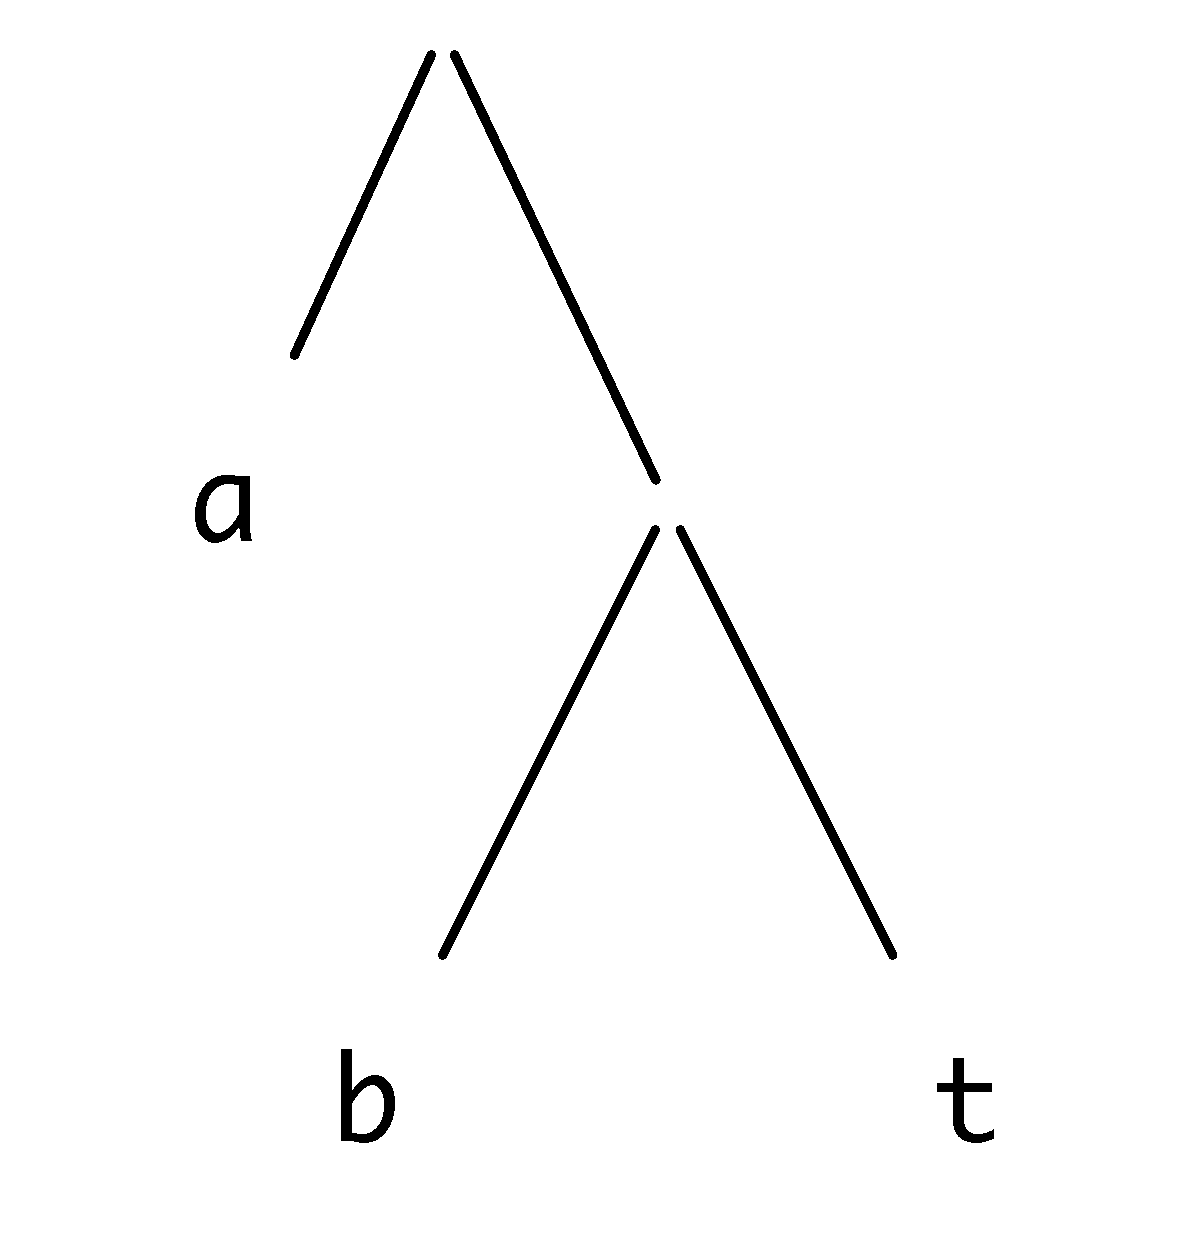
\includegraphics[width=1in]{Pictures/Huffman1.pdf}
\end{center}
We can see this as giving codes for the letters \texttt{a}, \texttt{b} and \texttt{t}
by looking at the \textbf{routes} taken to reach the letters. For example, to
get to \texttt{b}, we go {\em right\/} at the top node, and {\em left\/} at the
next: 
\begin{center}
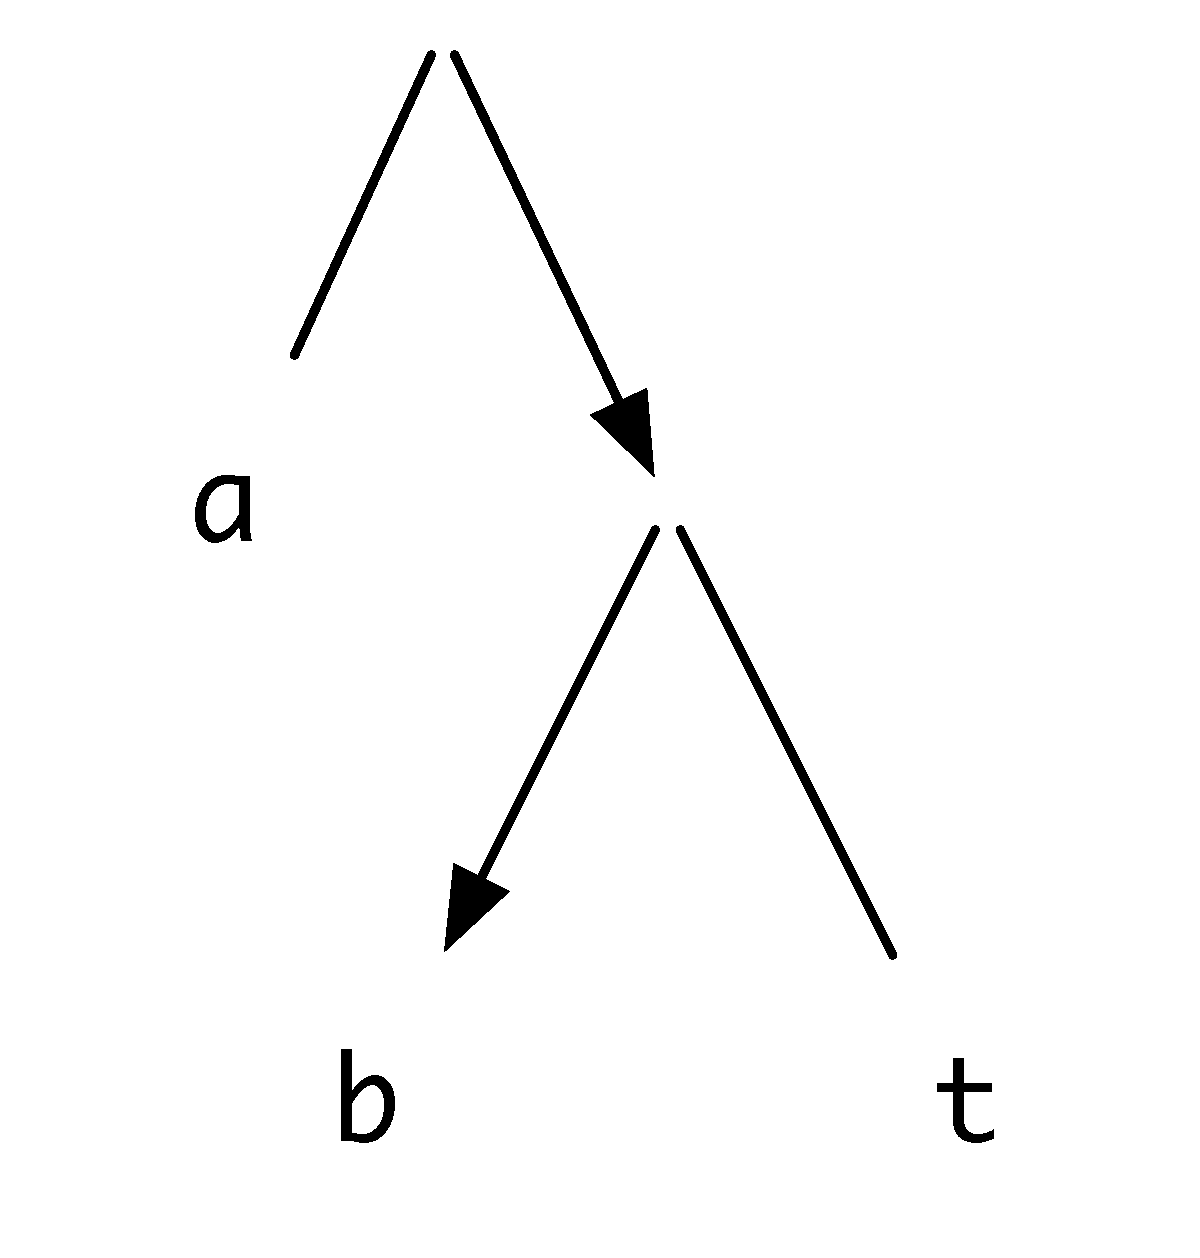
\includegraphics[width=1in]{Pictures/Huffman2.pdf}
\end{center}
which gives \texttt{b} the code \texttt{RL}. Similarly, \texttt{L} codes \texttt{a}, and
\texttt{RR} the letter \texttt{t}. 

The codes given by trees are  \textbf{prefix codes}\index{coding!prefix codes}; in these codes 
no code for a letter is the start (or prefix) of the code for another. This is
because no route to a leaf of the tree can be the start of the route to
another leaf. For more information about Huffman codes and
a wealth of general material on algorithms, see \citeN{cormen}.

A message is also \textbf{decoded} using the tree. Consider the message
\texttt{RLLRRRRLRR}. To decode we follow the route through the tree given,
moving right then left, to give the letter \texttt{b},
\begin{center}
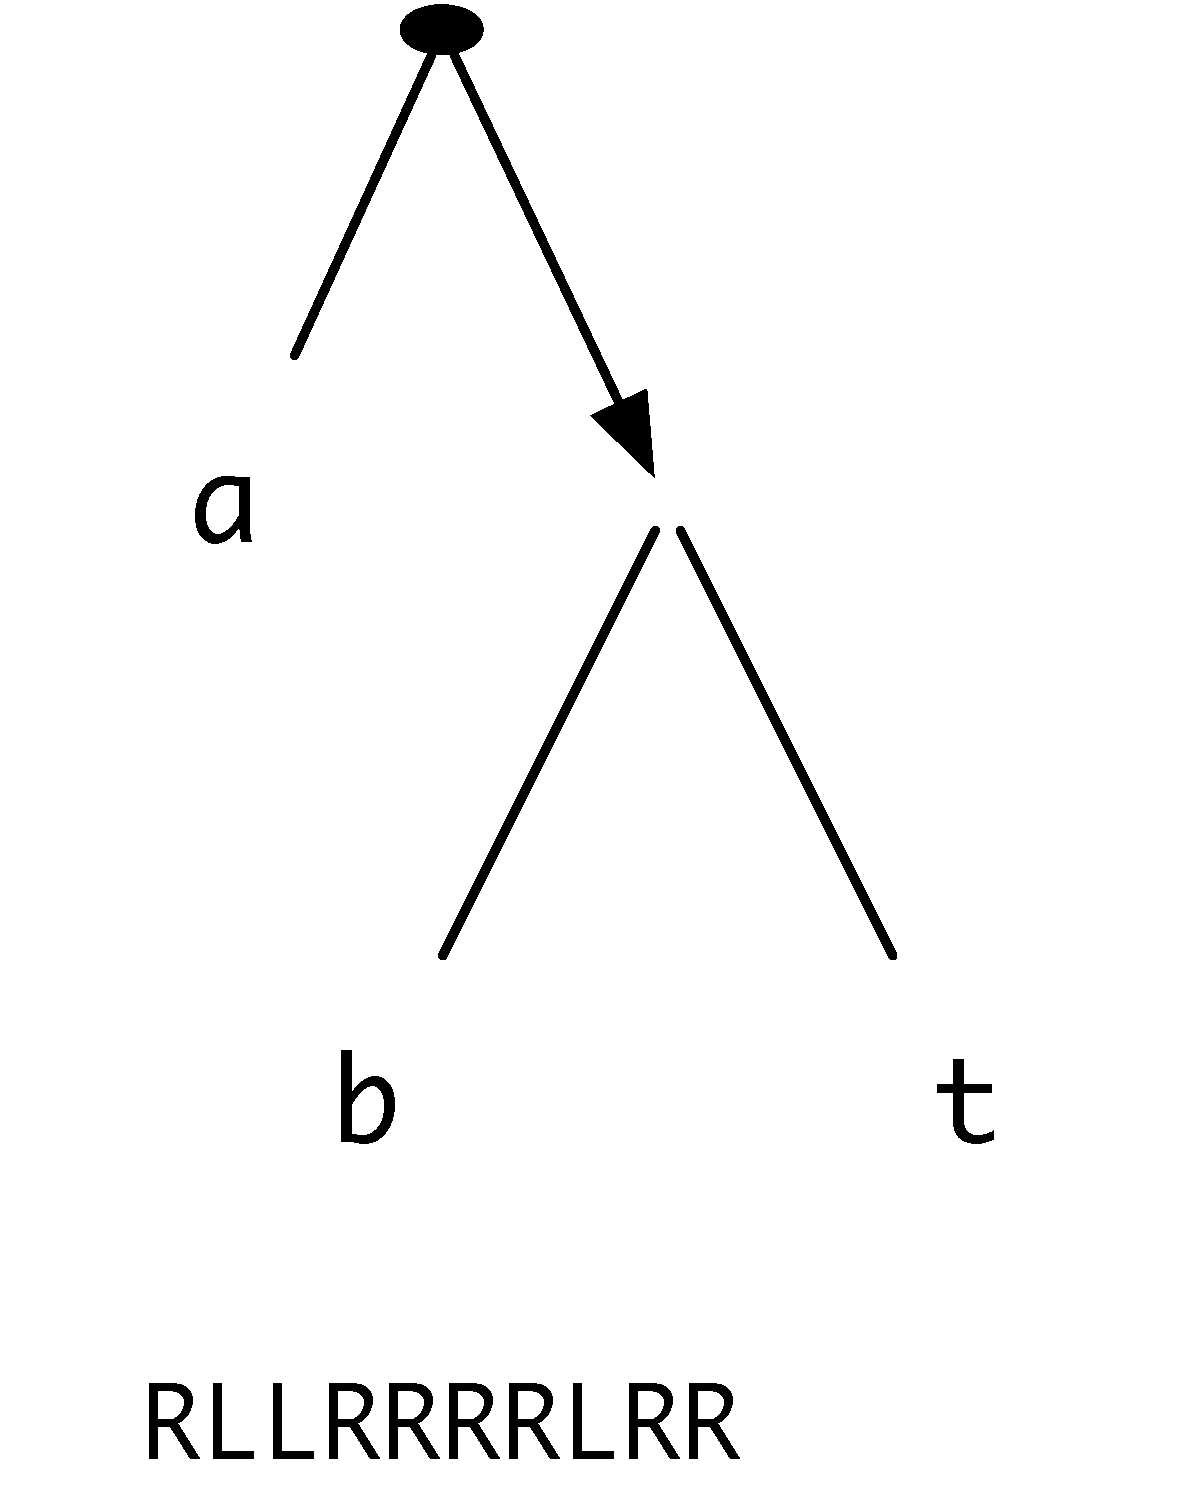
\includegraphics[width=1in]{Pictures/Huffman3.pdf}\hfill
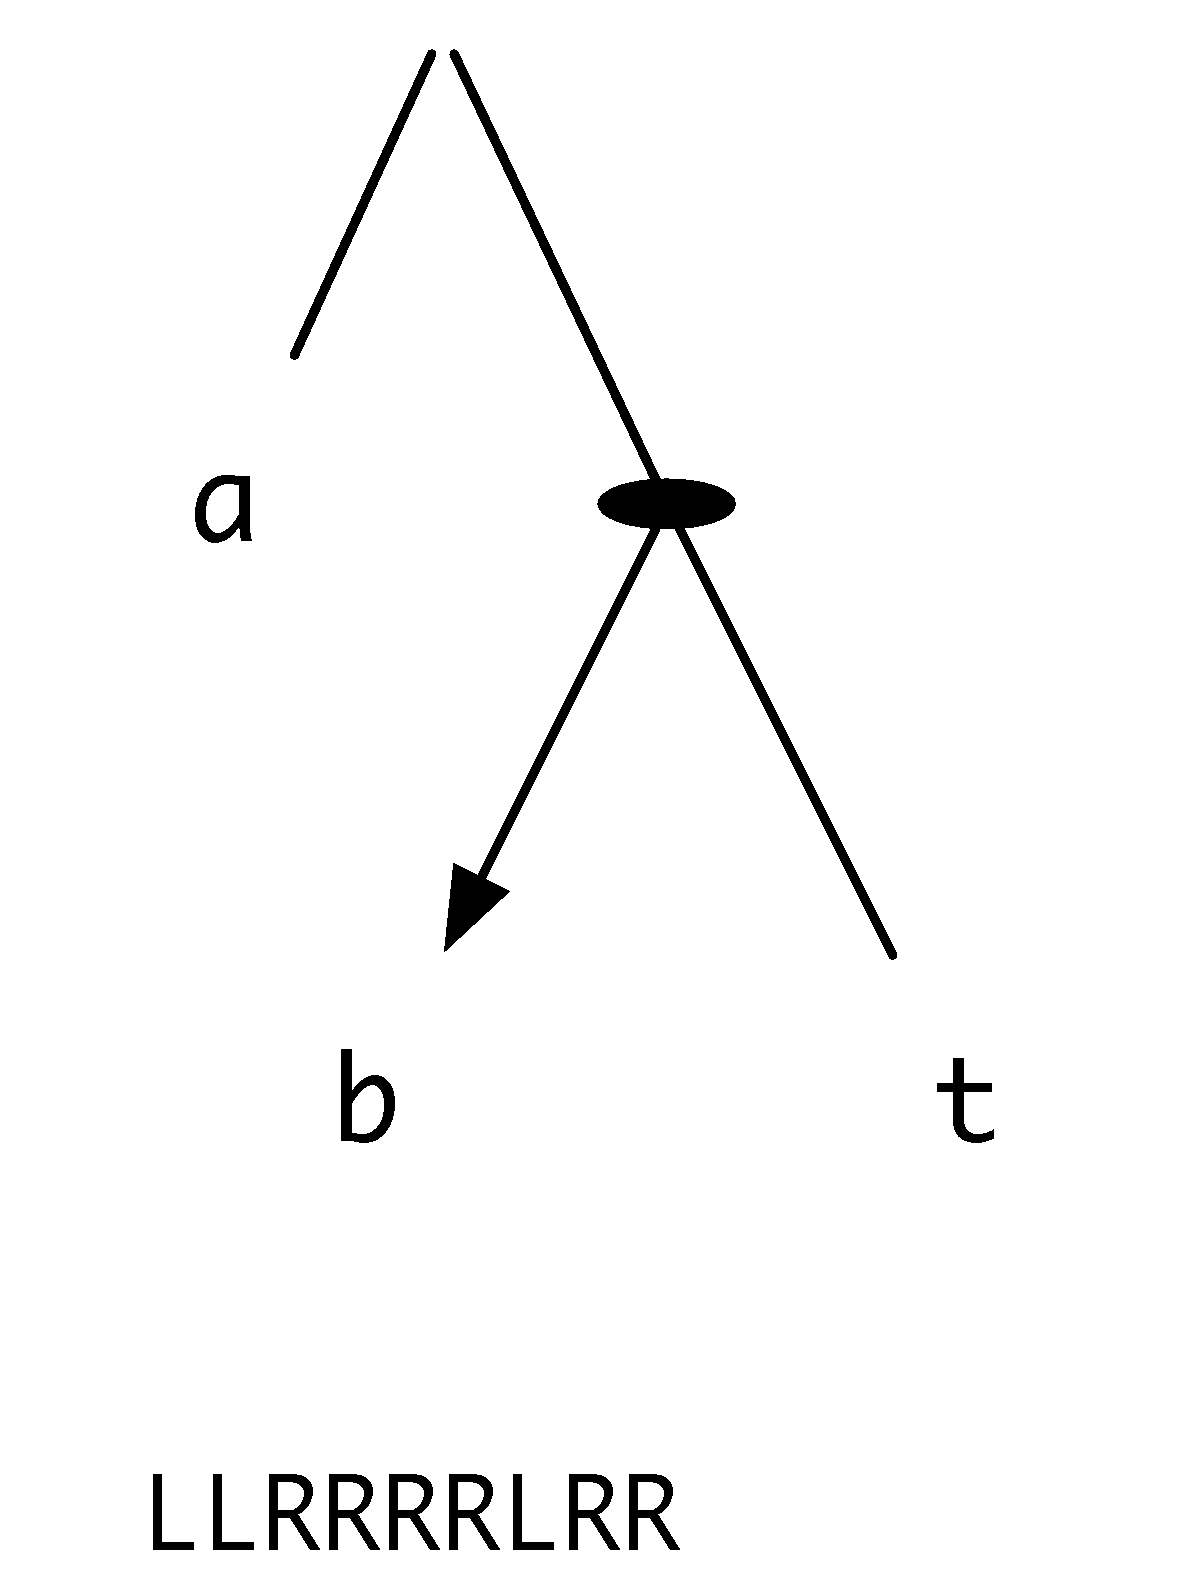
\includegraphics[width=1in]{Pictures/Huffman4.pdf}\hfill
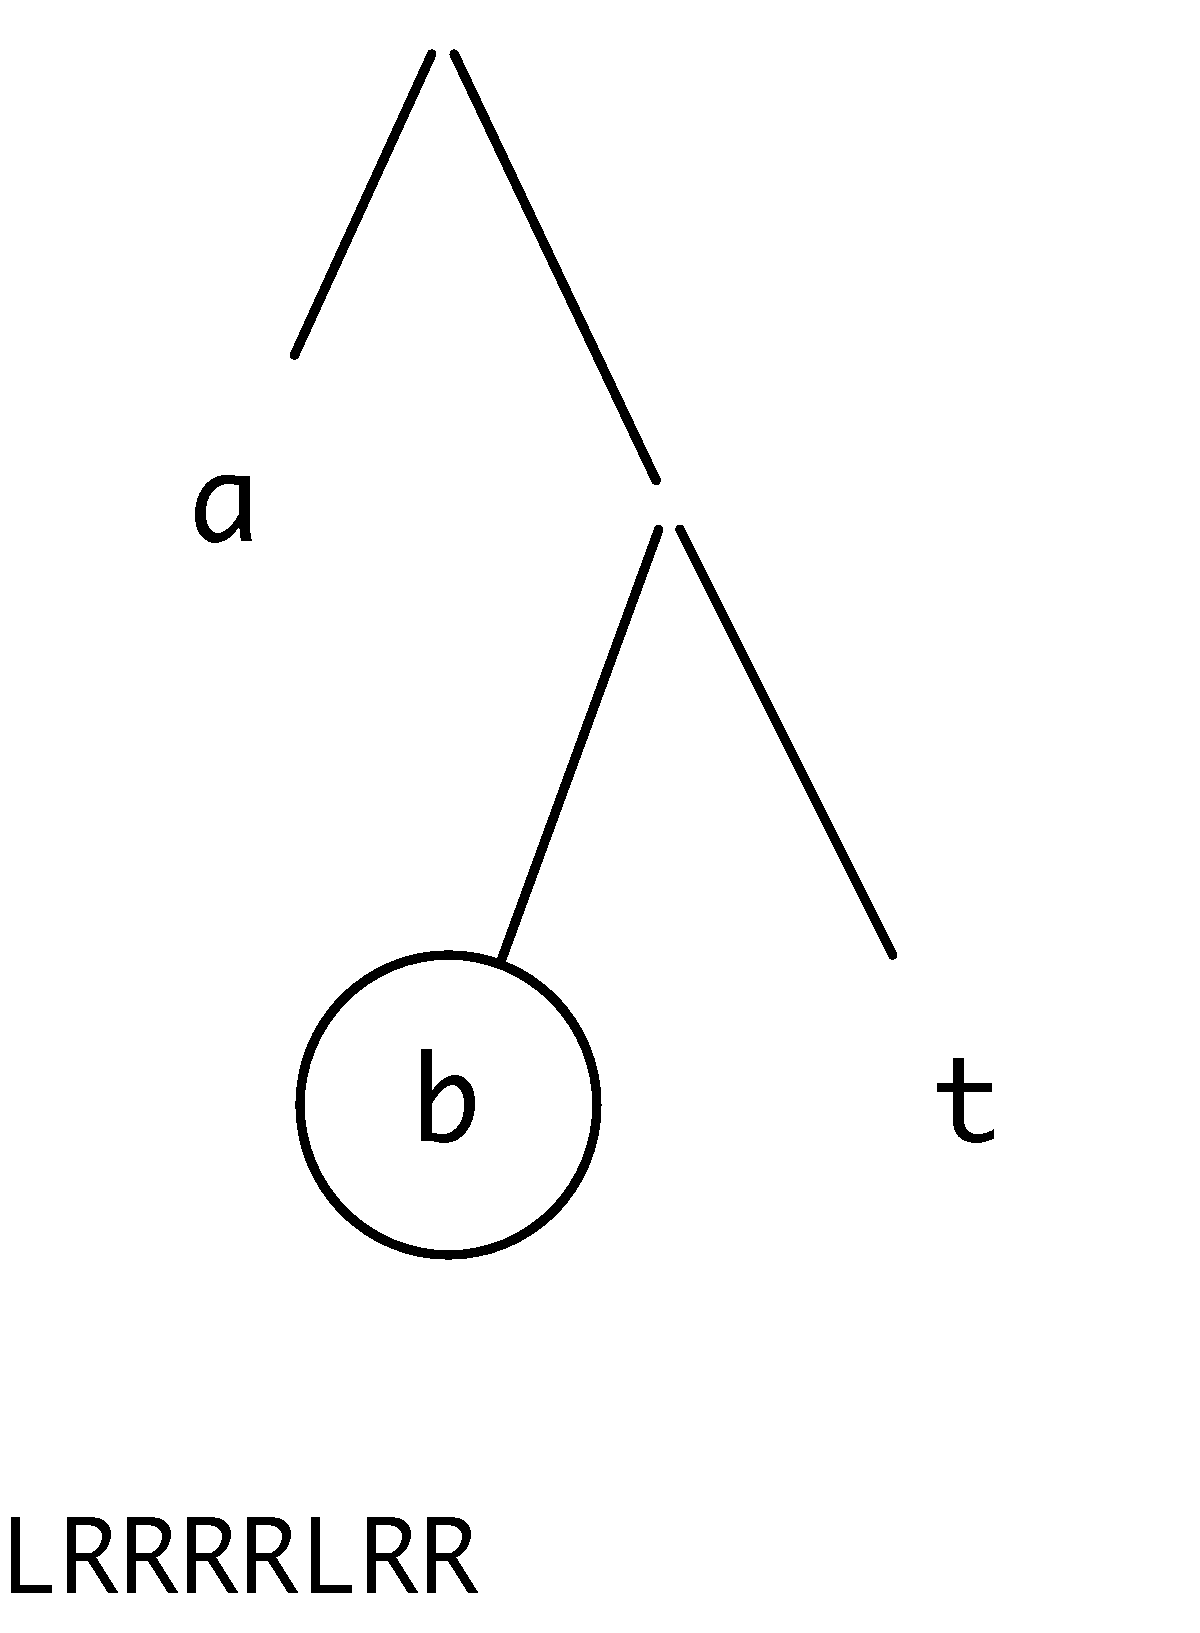
\includegraphics[width=1in]{Pictures/Huffman5.pdf}
\end{center}
where we have shown under each tree the sequence of bits remaining to be
decoded. Continuing again from the top, we have the codes for \texttt{a} then
\texttt{t},  
\begin{center}
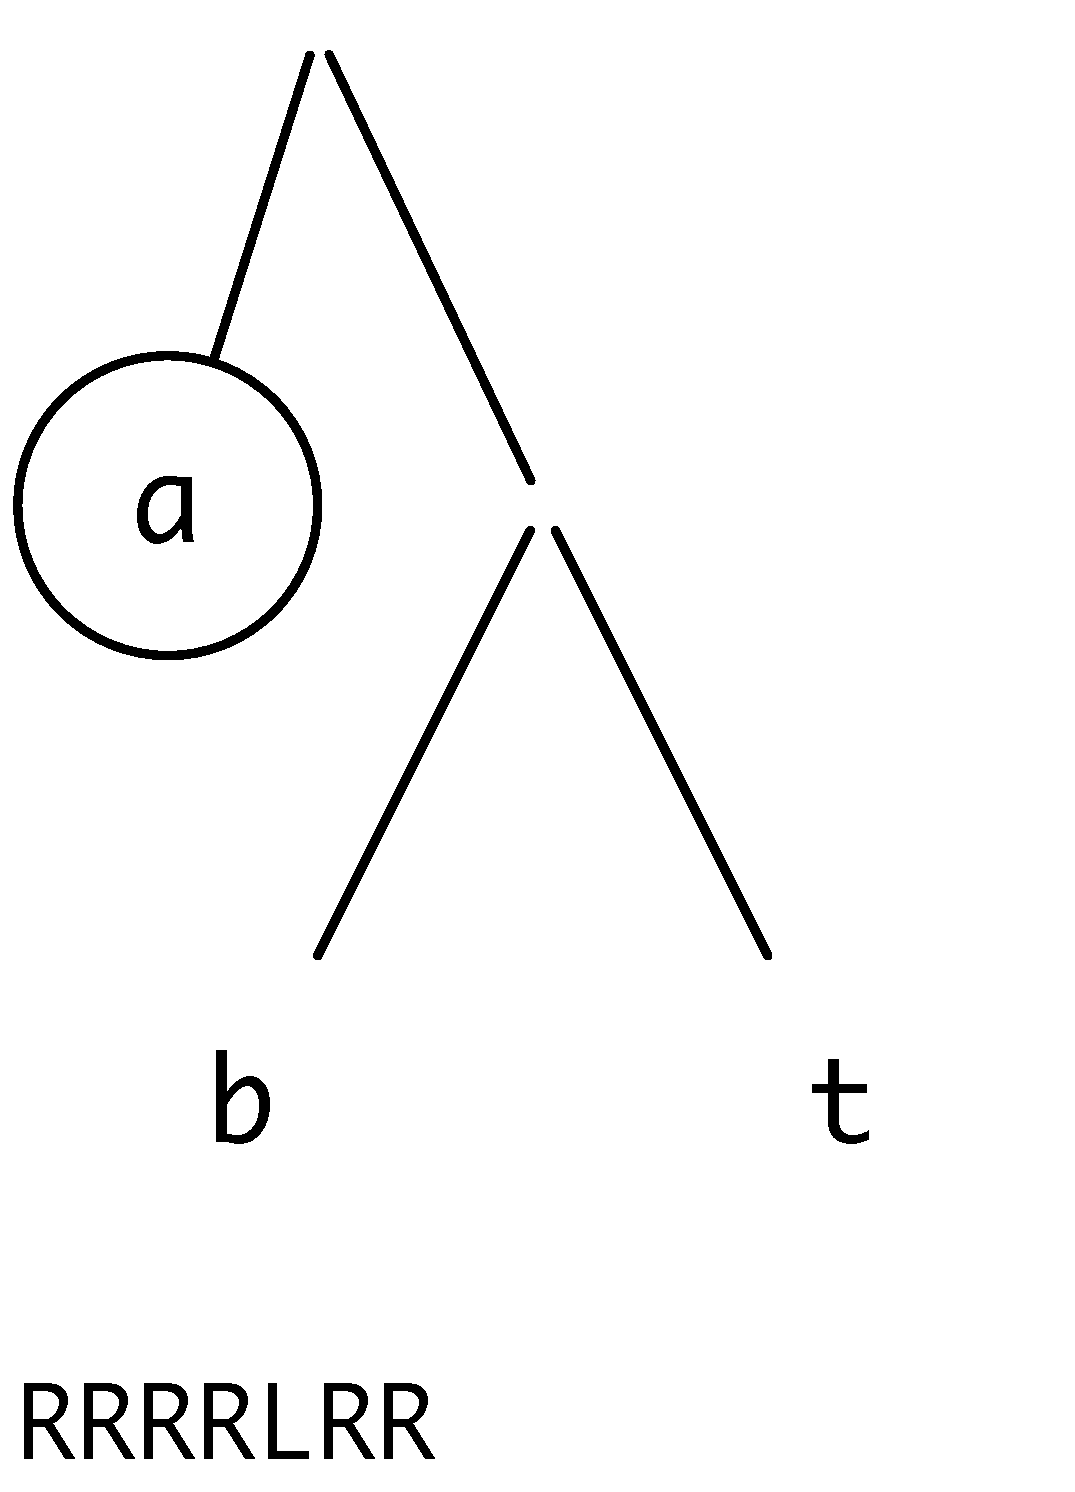
\includegraphics[width=1in]{Pictures/Huffman6.pdf}\hfill
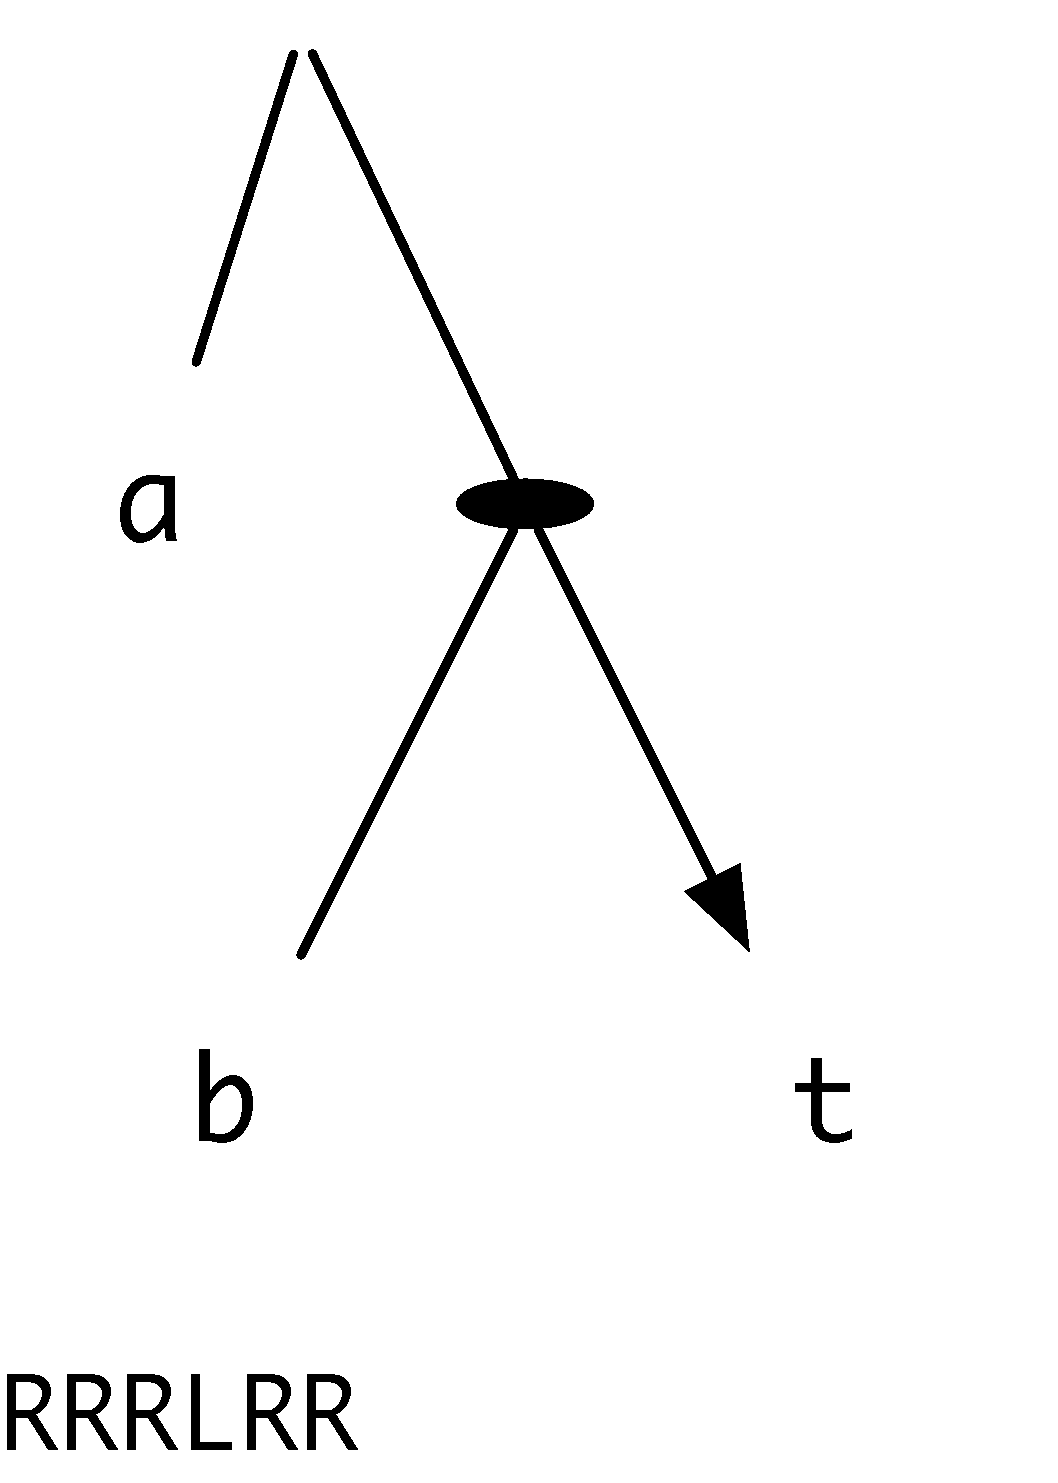
\includegraphics[width=1in]{Pictures/Huffman7.pdf}\hfill
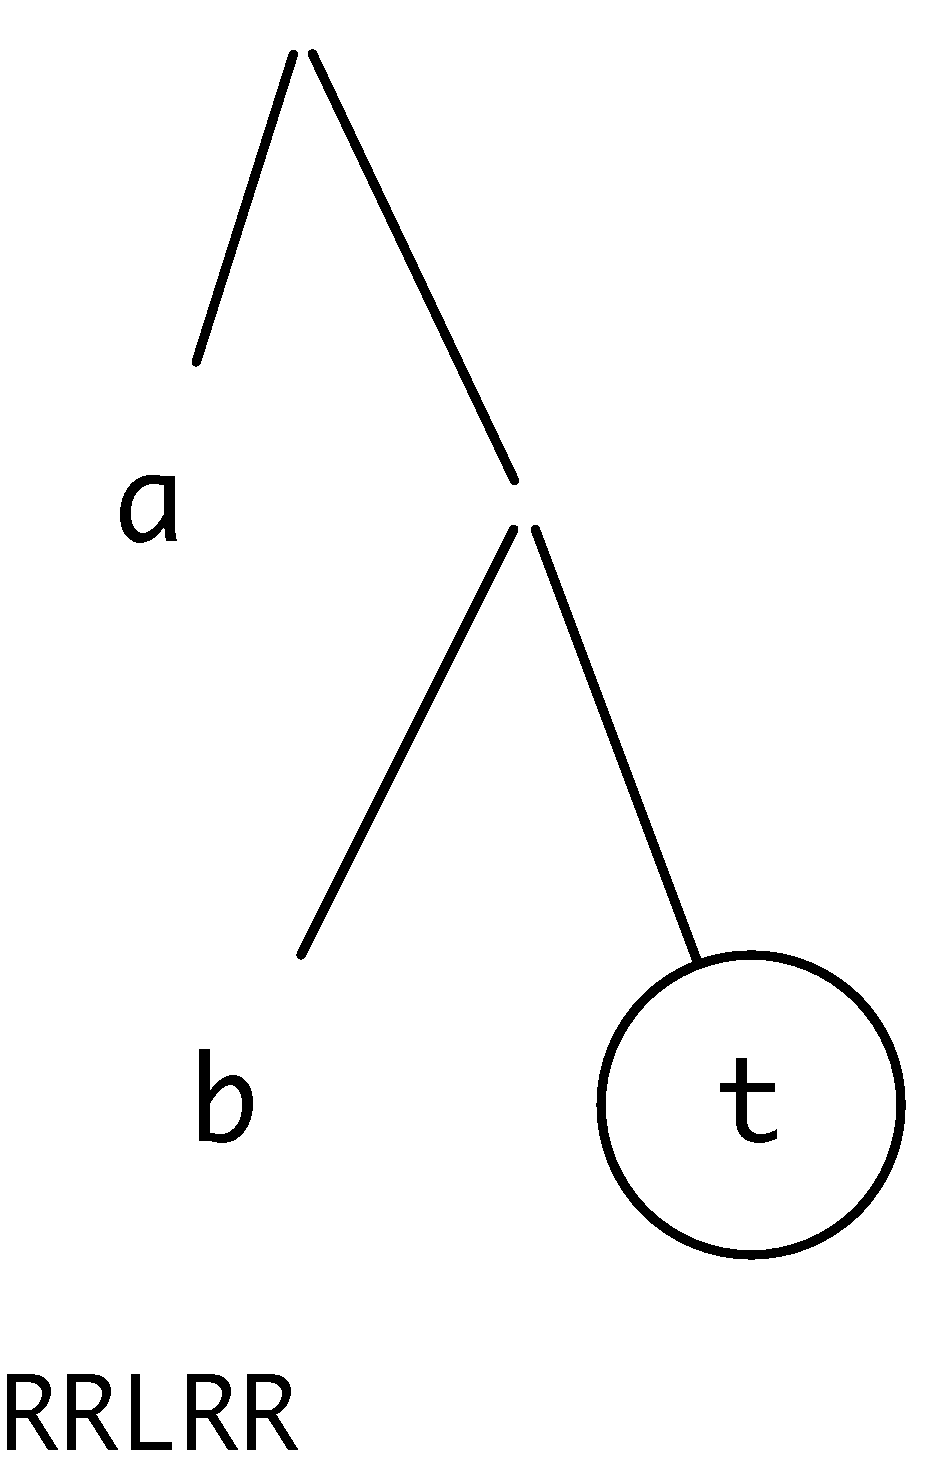
\includegraphics[width=0.9in]{Pictures/Huffman8.pdf}
\end{center}
so
the decoded message begins with the letters \texttt{bat}. 

In full, the message is \texttt{battat}, and the coded message is ten bits
long. The codes for individual characters are of different lengths; \texttt{a}
is coded in one bit, and the other characters in two. Is this a wise choice of
code in view of a message in which the letter \texttt{t} predominates? Using the
tree
\begin{center}
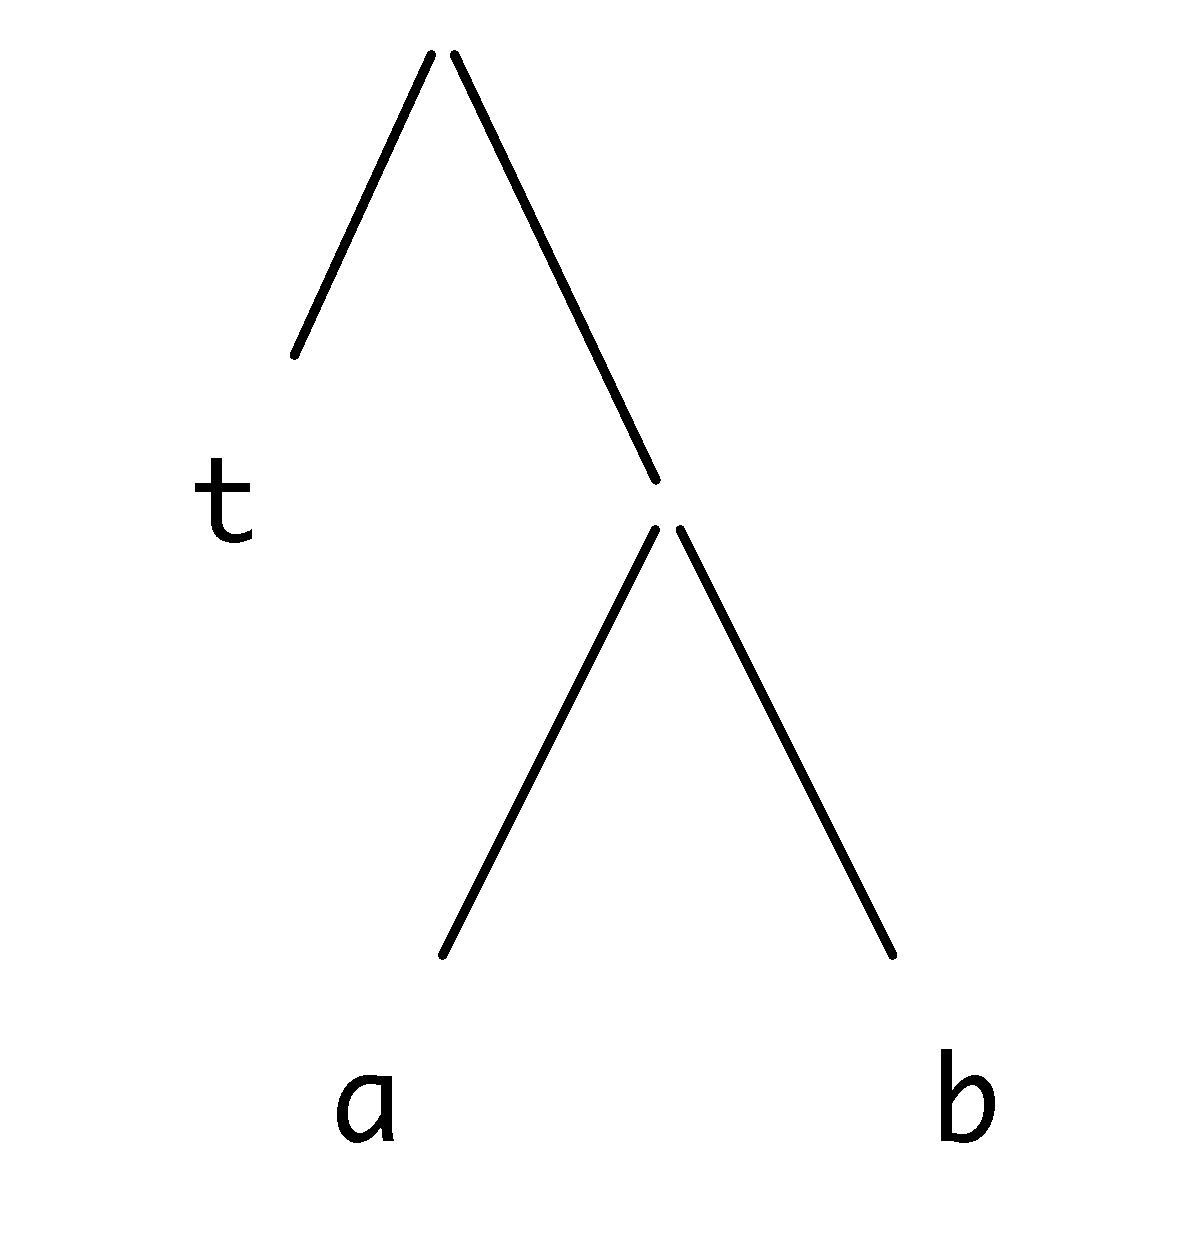
\includegraphics[width=1in]{Pictures/Huffman9.pdf}
\end{center}
the coded message becomes \texttt{RRRLLLRLL}, a nine-bit coding. A
Huffman\index{coding!Huffman} code is built so that the most frequent letters have the shortest
sequences of code bits, and the less frequent have more `expensive' code
sequences, justified by the rarity of their occurrence; Morse code is an
example of a Huffman code in common use.

The remainder of the chapter explores the implementation of Huffman coding,
illustrating the module system of Haskell.
\index{coding|)}

\begin{exercises}

\item
What is the coding of the message \texttt{battat} using the following
tree?
\begin{center}
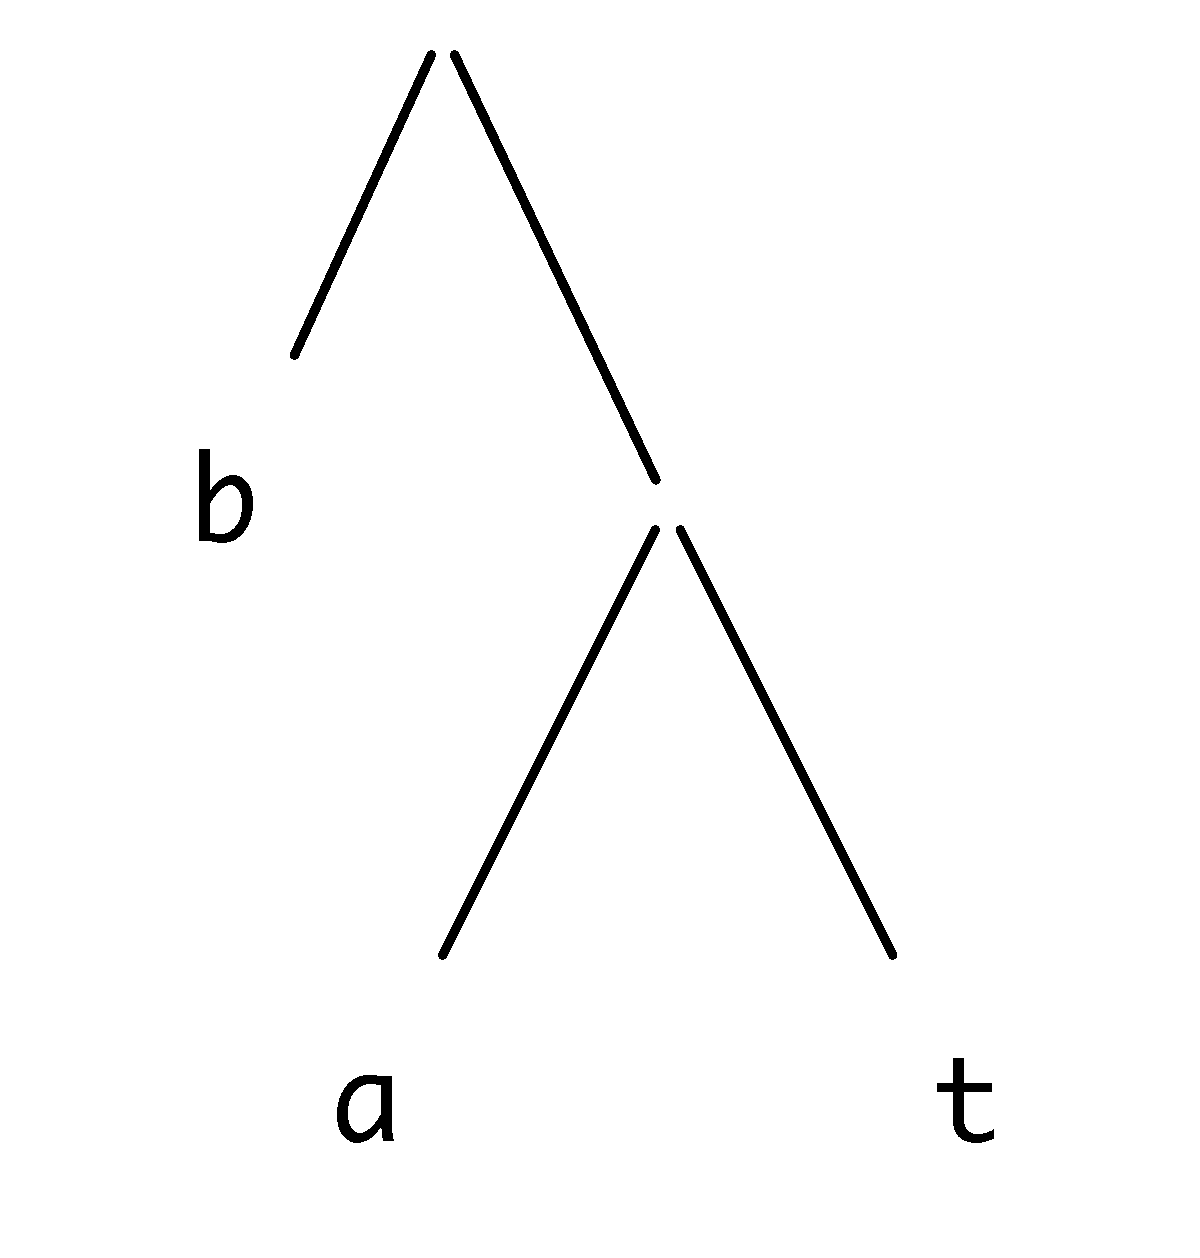
\includegraphics[width=1in]{Pictures/Huffman10.pdf}
\end{center}
Compare the length of the coding with the others given earlier. 

\item
Using the first coding tree, decode the coded
message \texttt{RLLRLRLLRR}. Which tree
would you expect to give the best coding of the message? Check your answer by
trying the three possibilities.
\end{exercises}


\section{Implementation -- I}

We now begin to implement the Huffman coding and decoding, in a series of
Haskell modules. The overall structure of the system we develop is illustrated
at the end of the chapter in Figure \ref{overallMod}. 

As earlier, we first develop the
types used in the system.

\subsection*{The types -- \texttt{Types.hs}}
\minx{Types.hs}

The codes are sequences of bits, so we define
\begin{alltt}
data Bit   =  L | R deriving (Eq,Show)\minx{Bit}\minx{HCode}
type HCode = [Bit]
\end{alltt}
and in the translation we will convert the Huffman tree to a table for ease
of coding.
\begin{alltt}
type Table = [ (Char,HCode) ]\minx{Table}
\end{alltt}
The Huffman trees themselves carry characters at the leaves. We shall see
presently that during their formation we also use information about the
frequency with which each character appears; hence the inclusion of 
integers
both at the leaves and at the internal nodes.
\begin{alltt}
data Tree = Leaf Char Int |\minx{Tree}
            Node Int Tree Tree
\end{alltt}
The file containing the module is illustrated in Figure
\ref{typeMod}.
\begin{figure}
\begin{alltt}
--         Types.hs							
--  
--         The types used in the Huffman coding example.			

-- The interface to the module Types is written out		
-- explicitly here, after the module name.                    	

module Types ( Tree(Leaf,Node), 
               Bit(L,R),  
               HCode , 
               Table  ) where

-- Trees to represent the relative frequencies of characters 	
-- and therefore the Huffman codes.						

data Tree = Leaf Char Int | Node Int Tree Tree

-- The types of bits, Huffman codes and tables of Huffman codes.	

data Bit = L | R deriving (Eq,Show)

type HCode = [Bit]

type Table = [ (Char,HCode) ]
\end{alltt}
\caption{The file \texttt{Types.hs}.}
\label{typeMod}
\end{figure}
The name of the file, with an indication of its purpose, is listed at the 
start of the file; each of the definitions is preceded by a comment as to its
purpose.

Note that we have given a full description of what is exported by the module,
by listing the items after the module name. For the \texttt{data} types which
are exported, \texttt{Tree} and 
\texttt{Bit}, the
constructors are exported explicitly; this could also be done by following their names
with \texttt{(..)}. 
This interface information could have been omitted, but we include it here as useful
documentation of the interface to the module.
\index{modules!interface documentation}

\subsection*{Coding and decoding -- \texttt{Coding.hs}}
\minx{Coding.hs}

This module uses the types in \texttt{Types.hs}, and so imports them like this
\begin{alltt}
\mbox{import Types ( Tree(Leaf,Node), Bit(L,R), HCode, Table )}
\end{alltt}
We have chosen to list the names imported here; the statement \texttt{import
Types} would have the same effect, but would lose the extra documentation.

The purpose of the module is to define functions to code and decode
messages: we export only these, and not the auxiliary function(s) which may
be used in their definition. Our module therefore has the header
\begin{alltt}
module Coding ( codeMessage , decodeMessage ) 
\end{alltt}
To code a message according to a table of
codes, we look up each character in the table, and concatenate the results.
\begin{alltt}
codeMessage :: Table -> [Char] -> HCode\minx{codeMessage}

codeMessage tbl = concat . map (lookupTable tbl)
\end{alltt}
It is interesting to see that the function level definition here gives an
exact implementation of the description which precedes it; using partial
application and function composition has made the definition clearer.

We now define \texttt{lookupTable}, which is a standard
function to look up the value corresponding to a `key' in a table.
\begin{alltt}
lookupTable :: Table -> Char -> HCode\minx{lookupTable}

lookupTable [] c = error "lookupTable"
lookupTable ((ch,n):tb) c
  | ch==c       = n
  | otherwise   = lookupTable tb c 
\end{alltt}
Because it is not included in the list of identifiers in the  \texttt{module} statement above, this definition is not exported.

To decode a message, which is a sequence of bits,  that is an element of
\texttt{HCode}, we use a \texttt{Tree}. 
\begin{alltt}
decodeMessage :: Tree -> HCode -> [Char]\minx{decodeMessage}
\end{alltt}
We saw in Section \ref{codeIntro} that decoding according to the tree \texttt{tr}
has two main cases. 
\begin{titemize}
\item If we are at an internal \texttt{Node}, we choose the sub-tree dictated by
the first bit of the code.
\item If at a leaf, we read off the character found, and then begin to decode
the remainder of the code at the top of the tree \texttt{tr}.
\end{titemize}
When the code is exhausted, so is the decoded message.
\begin{alltt}
decodeMessage tr
  = decodeByt tr
    where
    decodeByt (Node n t1 t2) (L:rest)
      = decodeByt t1 rest
    decodeByt (Node n t1 t2) (R:rest)
      = decodeByt t2 rest
    decodeByt (Leaf c n) rest
      = c : decodeByt tr rest
    decodeByt t [] = []
\end{alltt}
The locally defined function is called \texttt{decodeByt} because it decodes `by
\texttt{t}'.

The first coding tree and example message of Section \ref{codeIntro} can be
given by
\begin{alltt}
exam1 = Node 0 (Leaf 'a' 0)
               (Node 0 (Leaf 'b' 0) (Leaf 't' 0))
mess1 = [R,L,L,R,R,R,R,L,R,R]
\end{alltt}
and decoding of this message begins thus
\begin{alltt}
decodeMessage exam1 mess1
\step decodeByt exam1 mess1
\step decodeByt exam1 [R,L,L,R,R,R,R,L,R,R]
\step decodeByt (Node 0 (Leaf 'b' 0) (Leaf 't' 0)) 
                                 [L,L,R,R,R,R,L,R,R]
\step decodeByt (Leaf 'b' 0) [L,R,R,R,R,L,R,R]
\step 'b' : decodeByt exam1 [L,R,R,R,R,L,R,R] 
\step 'b' : decodeByt (Leaf 'a' 0) [R,R,R,R,L,R,R]
\step 'b' : 'a' : decodeByt exam1 [R,R,R,R,L,R,R] 
\end{alltt}
Before looking at the implementation any further, we look at how to construct
the Huffman coding tree, given a text.

\begin{exercises}

\item
Complete the calculation of \texttt{decodeMessage exam1 mess1} begun above.

\item
With the table
\begin{alltt}
table1 = [ ('a',[L]) , ('b',[R,L]) , ('t',[R,R]) ]
\end{alltt}
give a calculation of 
\begin{alltt}
codeMessage table1 "battab"
\end{alltt}
\end{exercises}
\section{Building Huffman trees}
%\index{Huffman trees!building}

Given a text, such as \texttt{"battat"}, how do we find the tree giving the
optimal code for the text? We explain it in a number of
stages following Section 17.3
of \citeN{cormen}.
\begin{titemize} 
\item We first find the frequencies of the
individual letters, in this case giving
\begin{alltt}
[('b',1),('a',2),('t',3)]
\end{alltt}
\item The main idea of the translation is to build the tree by taking the two
characters occurring least frequently, and making a {\em single\/} character
(or {\em tree\/}) of them. This process is repeated until a single tree
results; the steps which follow give this process in more detail.
\item Each of \texttt{('b',1)}, \ldots\ is turned into a tree, giving the list of
trees
\begin{alltt}
[ Leaf 'b' 1 , Leaf 'a' 2 , Leaf 't' 3 ]
\end{alltt}
which is sorted into frequency order.
\item We then begin to {\em amalgamate together\/} trees: we take the two
trees of lowest frequency, put them together, and insert the result in the
appropriate place to preserve the frequency order.
\begin{alltt}
[ Node 3 (Leaf 'b' 1) (Leaf 'a' 2) , Leaf 't' 3 ]
\end{alltt}
\item This process is repeated, until a single tree results
\begin{alltt}
Node 6 (Node 3 (Leaf 'b' 1) (Leaf 'a' 2)) (Leaf 't' 3)
\end{alltt}
which is pictured like this
\begin{center}
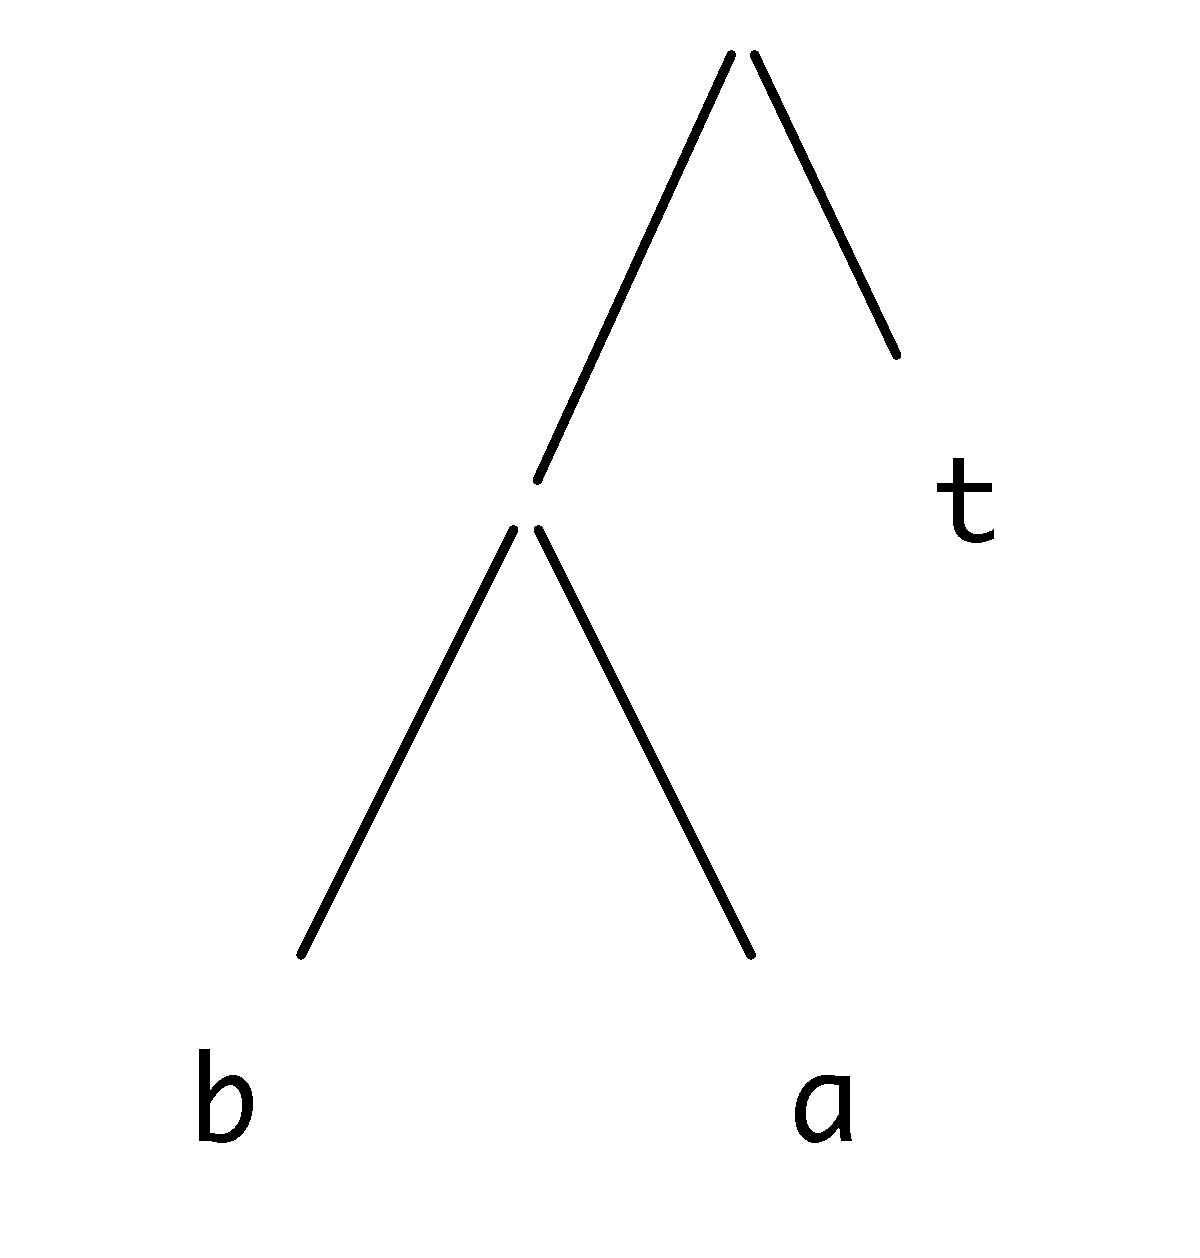
\includegraphics[width=1in]{Pictures/Huffman11.pdf}
\end{center}
\item This tree can then be turned into a \texttt{Table}
\begin{alltt}
[ ('b',[L,L]) , ('a',[L,R]) , ('t',[R]) ]
\end{alltt}
\end{titemize}
We now look at how the system is implemented in Haskell.

\section{Design}
\index{design!Huffman coding system}

Implementing the system will involve us in designing various modules to
perform the stages given above. We start by deciding what the modules will
be  and the functions that they will implement. This is the equivalent at the
larger scale of \textbf{divide and conquer}\index{divide and conquer};
we separate the problem into
manageable portions, which can be solved separately, and which are put
together using the \texttt{import} and \texttt{module} statements. We design
these \textbf{interfaces} \index{interface}before implementing the functions.

The three stages of conversion are summarized in Figure \ref{codeDesign},
which shows the module directives of the three component files. We have added
as comments the types of objects to be exported, so that these directives
contain enough information for the exported functions in the
files to be used without knowing {\em how\/} they are defined. 

\begin{figure}\begin{alltt}
Frequency.hs:

module Frequency ( frequency )  -- [Char] -> [(Char,Int)]

\hrulefill

MakeTree.hs:

module MakeTree ( makeTree )    -- [(Char,Int)] -> Tree
import Types

\hrulefill

CodeTable.hs:

module CodeTable ( codeTable )  -- Tree -> Table
import Types 
\end{alltt}
\caption{Module directives for Huffman tree formation.}
\label{codeDesign}
\end{figure}
In fact the component functions \texttt{frequency} and \texttt{makeTree} will
never be used separately, and so we compose them in the module 
\texttt{MakeCode.hs} when bringing the three files together. This is given in Figure
\ref{makeCode}.

\begin{figure}
\begin{alltt}
-- 								
--         MakeCode.hs							
-- 								
--         Huffman coding in Haskell.					
-- 								

module MakeCode ( codes, codeTable ) where

import Types
import Frequency ( frequency )
import MakeTree  ( makeTree )
import CodeTable ( codeTable )

-- Putting together frequency calculation and tree conversion	

codes :: [Char] -> Tree

codes = makeTree . frequency
\end{alltt}
\caption{The module \texttt{MakeCode.hs}.}
\label{makeCode}
\end{figure}
Our next task is to implement each module in full and we turn to that now.

\section{Implementation -- II}

In this section we discuss in turn the three implementation modules.

\subsection*{Counting characters --- \texttt{Frequency.hs}}
\minx{Frequency.hs}

The aim of the function \texttt{frequency}\minx{frequency} is to take a text such as 
\texttt{"battat"} to a list of characters, in increasing frequency of occurrence,
\texttt{[('b',1),('a',2),('t',3)]}. We do this in three stages:
\begin{titemize}
\item First we pair each character with the count of \texttt{1}, giving
\begin{alltt}
[('b',1),('a',1),('t',1),('t',1),('a',1),('t',1)]
\end{alltt}
\item Next, we sort the list on the characters, bringing together the counts of
equal characters.
\begin{alltt}
[('a',2),('b',1),('t',3)]
\end{alltt}
\item Finally, we sort the list into increasing frequency order, to give the
list above.
\end{titemize}
The function uses two different sorts -- one on character, one on
frequency -- to achieve its result. Is there any way we can define a single
sorting function to perform both sorts? 

We can give a general merge sort
\index{sorting!merge sort}
function, which works by \textbf{merging}, in order, the results of sorting the
front and rear halves of the list.
\begin{alltt}
mergeSort :: ([a]->[a]->[a]) -> [a] -> [a]\minx{mergeSort}

mergeSort merge xs
  | length xs < 2 	= xs					
  | otherwise		
      = merge (mergeSort merge first)
              (mergeSort merge second)	
        where
        first  = take half xs
        second = drop half xs
        half   = (length xs) `div` 2
\end{alltt}
The first argument to \texttt{mergeSort} is the merging function, which takes
two sorted lists and merges their contents in order. It is by making this
operation a {\em parameter\/} that the \texttt{mergeSort} function becomes
reusable.

In sorting the characters, we amalgamate entries for the same character
\begin{alltt}\minx{alphaMerge}
alphaMerge :: [(Char,Int)] -> [(Char,Int)] -> [(Char,Int)]	

alphaMerge xs [] = xs
alphaMerge [] ys = ys
alphaMerge ((p,n):xs) ((q,m):ys)
  | (p==q)      = (p,n+m) : alphaMerge xs ys		
  | (p<q)       = (p,n) : alphaMerge xs ((q,m):ys)	
  | otherwise   = (q,m) : alphaMerge ((p,n):xs) ys	
\end{alltt}
while when sorting on frequency we compare frequencies; when two
pairs have the same frequency, we order according to the character ordering.
\begin{alltt}\minx{freqMerge}
freqMerge :: [(Char,Int)] -> [(Char,Int)] -> [(Char,Int)]	

freqMerge xs [] = xs
freqMerge [] ys = ys
freqMerge ((p,n):xs) ((q,m):ys)
  | (n<m || (n==m && p<q)) 
    = (p,n) : freqMerge xs ((q,m):ys)	
  | otherwise 
    = (q,m) : freqMerge ((p,n):xs) ys	
\end{alltt}
We can now give the top-level definition of \texttt{frequency}
\begin{alltt}
frequency :: [Char] -> [ (Char,Int) ]\minx{frequency}

frequency
  = mergeSort freqMerge . mergeSort alphaMerge . map start
    where
    start ch = (ch,1)
\end{alltt}
which we can see is a direct combination of the three stages listed in the
informal description of the algorithm.

Note that of all the functions defined in this module, only \texttt{frequency}
is exported.

\subsection*{Making the Huffman tree -- \texttt{MakeTree.hs}}
\minx{MakeTree.hs}

We have two stages in making a Huffman tree from a list of characters with
their frequencies.
\begin{alltt}
makeTree :: [ (Char,Int) ] -> Tree\minx{makeTree}
makeTree  = makeCodes . toTreeList
\end{alltt}
where
\begin{alltt}\minx{toTreeList}\minx{makeCodes}
toTreeList :: [ (Char,Int) ] -> [Tree]
makeCodes  :: [Tree] -> Tree
\end{alltt}
The function \texttt{toTreeList} converts each character-number pair into a
tree, thus
\begin{alltt}
toTreeList = map (uncurry Leaf)
\end{alltt}
where note that we use the prelude function \texttt{uncurry} to make an uncurried version
of the constructor function \texttt{Leaf}.

The function \texttt{makeCodes} amalgamates trees successively into a single
tree
\begin{alltt}
makeCodes [t] = t
makeCodes ts  = makeCodes (amalgamate ts)
\end{alltt}
How are trees amalgamated? We have to pair together the first two trees in
the list (since the list is kept in ascending order of frequency) and then
insert the result in the list preserving the frequency order. Working top-down, we have 
\begin{alltt}
amalgamate :: [ Tree ] -> [ Tree ]

amalgamate (t1:t2:ts) = insTree (pair t1 t2) ts
\end{alltt}
When we pair two trees, we need to combine their frequency counts, so
\begin{alltt}
pair :: Tree -> Tree -> Tree

pair t1 t2 = Node (v1+v2) t1 t2
             where
             v1 = value t1
             v2 = value t2
\end{alltt}
where the value of a tree is given by
\begin{alltt}
value :: Tree -> Int

value (Leaf _ n)   = n
value (Node n _ _) = n
\end{alltt}
The definition of \texttt{insTree}, which is similar to that used in an insertion
sort, is left as an exercise. Again, the definition of the exported function
uses various others whose definitions are not visible to the `outside world'.

\subsection*{The code table -- \texttt{CodeTable.hs}}
\minx{CodeTable.hs}

Here we give the function \texttt{codeTable} which takes a Huffman tree into a
code table. In converting the tree \texttt{Node n t1 t2} we have to convert 
\texttt{t1}, adding \texttt{L} at the front of the code, and \texttt{t2} with \texttt{R} at
the head. We therefore write the more general conversion function
\begin{alltt}
convert :: HCode -> Tree -> Table\minx{convert}
\end{alltt}
whose first argument is the `path so far' into the tree. The definition is
\begin{alltt}
convert cd (Leaf c n) 
      =  [(c,cd)]
convert cd (Node n t1 t2)
      = (convert (cd++[L]) t1) ++ (convert (cd++[R]) t2)
\end{alltt}
The \texttt{codeTable} function is given by starting the conversion with an
empty code string
\begin{alltt}\minx{codeTable}
codeTable :: Tree -> Table
codeTable = convert []
\end{alltt}
Consider the calculation of
\begin{alltt}
codeTable (Node 6 (Node 3 (Leaf 'b' 1) (Leaf 'a' 2)) 
                  (Leaf 't' 3))
\step convert [] (Node 6 (Node 3 (Leaf 'b' 1) (Leaf 'a' 2)) 
                       (Leaf 't' 3))
\step convert [L] (Node 3 (Leaf 'b' 1) (Leaf 'a' 2)) ++
    convert [R] (Leaf 't' 3)
\step convert [L,L] (Leaf 'b' 1) ++ 
    convert [L,R] (Leaf 'a' 2) ++ 
    [ ('t',[R]) ]
\step [ ('b',[L,L]) , ('a',[L,R]) , ('t',[R]) ]
\end{alltt}

\begin{figure}[t]
\begin{center}
\begin{alltt}
-- The main module of the Huffman example

module Main (main, codeMessage, decodeMessage, codes, codeTable ) where

import Types    ( Tree(Leaf,Node), Bit(L,R), HCode , Table )
import Coding   ( codeMessage, decodeMessage ) 
import MakeCode ( codes, codeTable )

-- Main expression: print the coded and decoded 
-- example text "there is a green hill".
main = print decoded

-- The example message to be coded.
message :: String
message = "there are green hills here"

-- The Huffman tree generated from the example.
treeEx :: Tree
treeEx = codes "there is a green hill"

-- The coding table generated from the example.					
tableEx :: Table
tableEx = codeTable (codes "there is a green hill")

-- The example in code.
coded :: HCode
coded = codeMessage tableEx message

-- The example coded and then decoded.
decoded :: String
decoded = decodeMessage treeEx coded
\end{alltt}
\end{center}
\caption{The \texttt{Main} module of the Huffman coding system.}
\label{mainMod}
\end{figure}


\begin{figure}[t]
\begin{center}
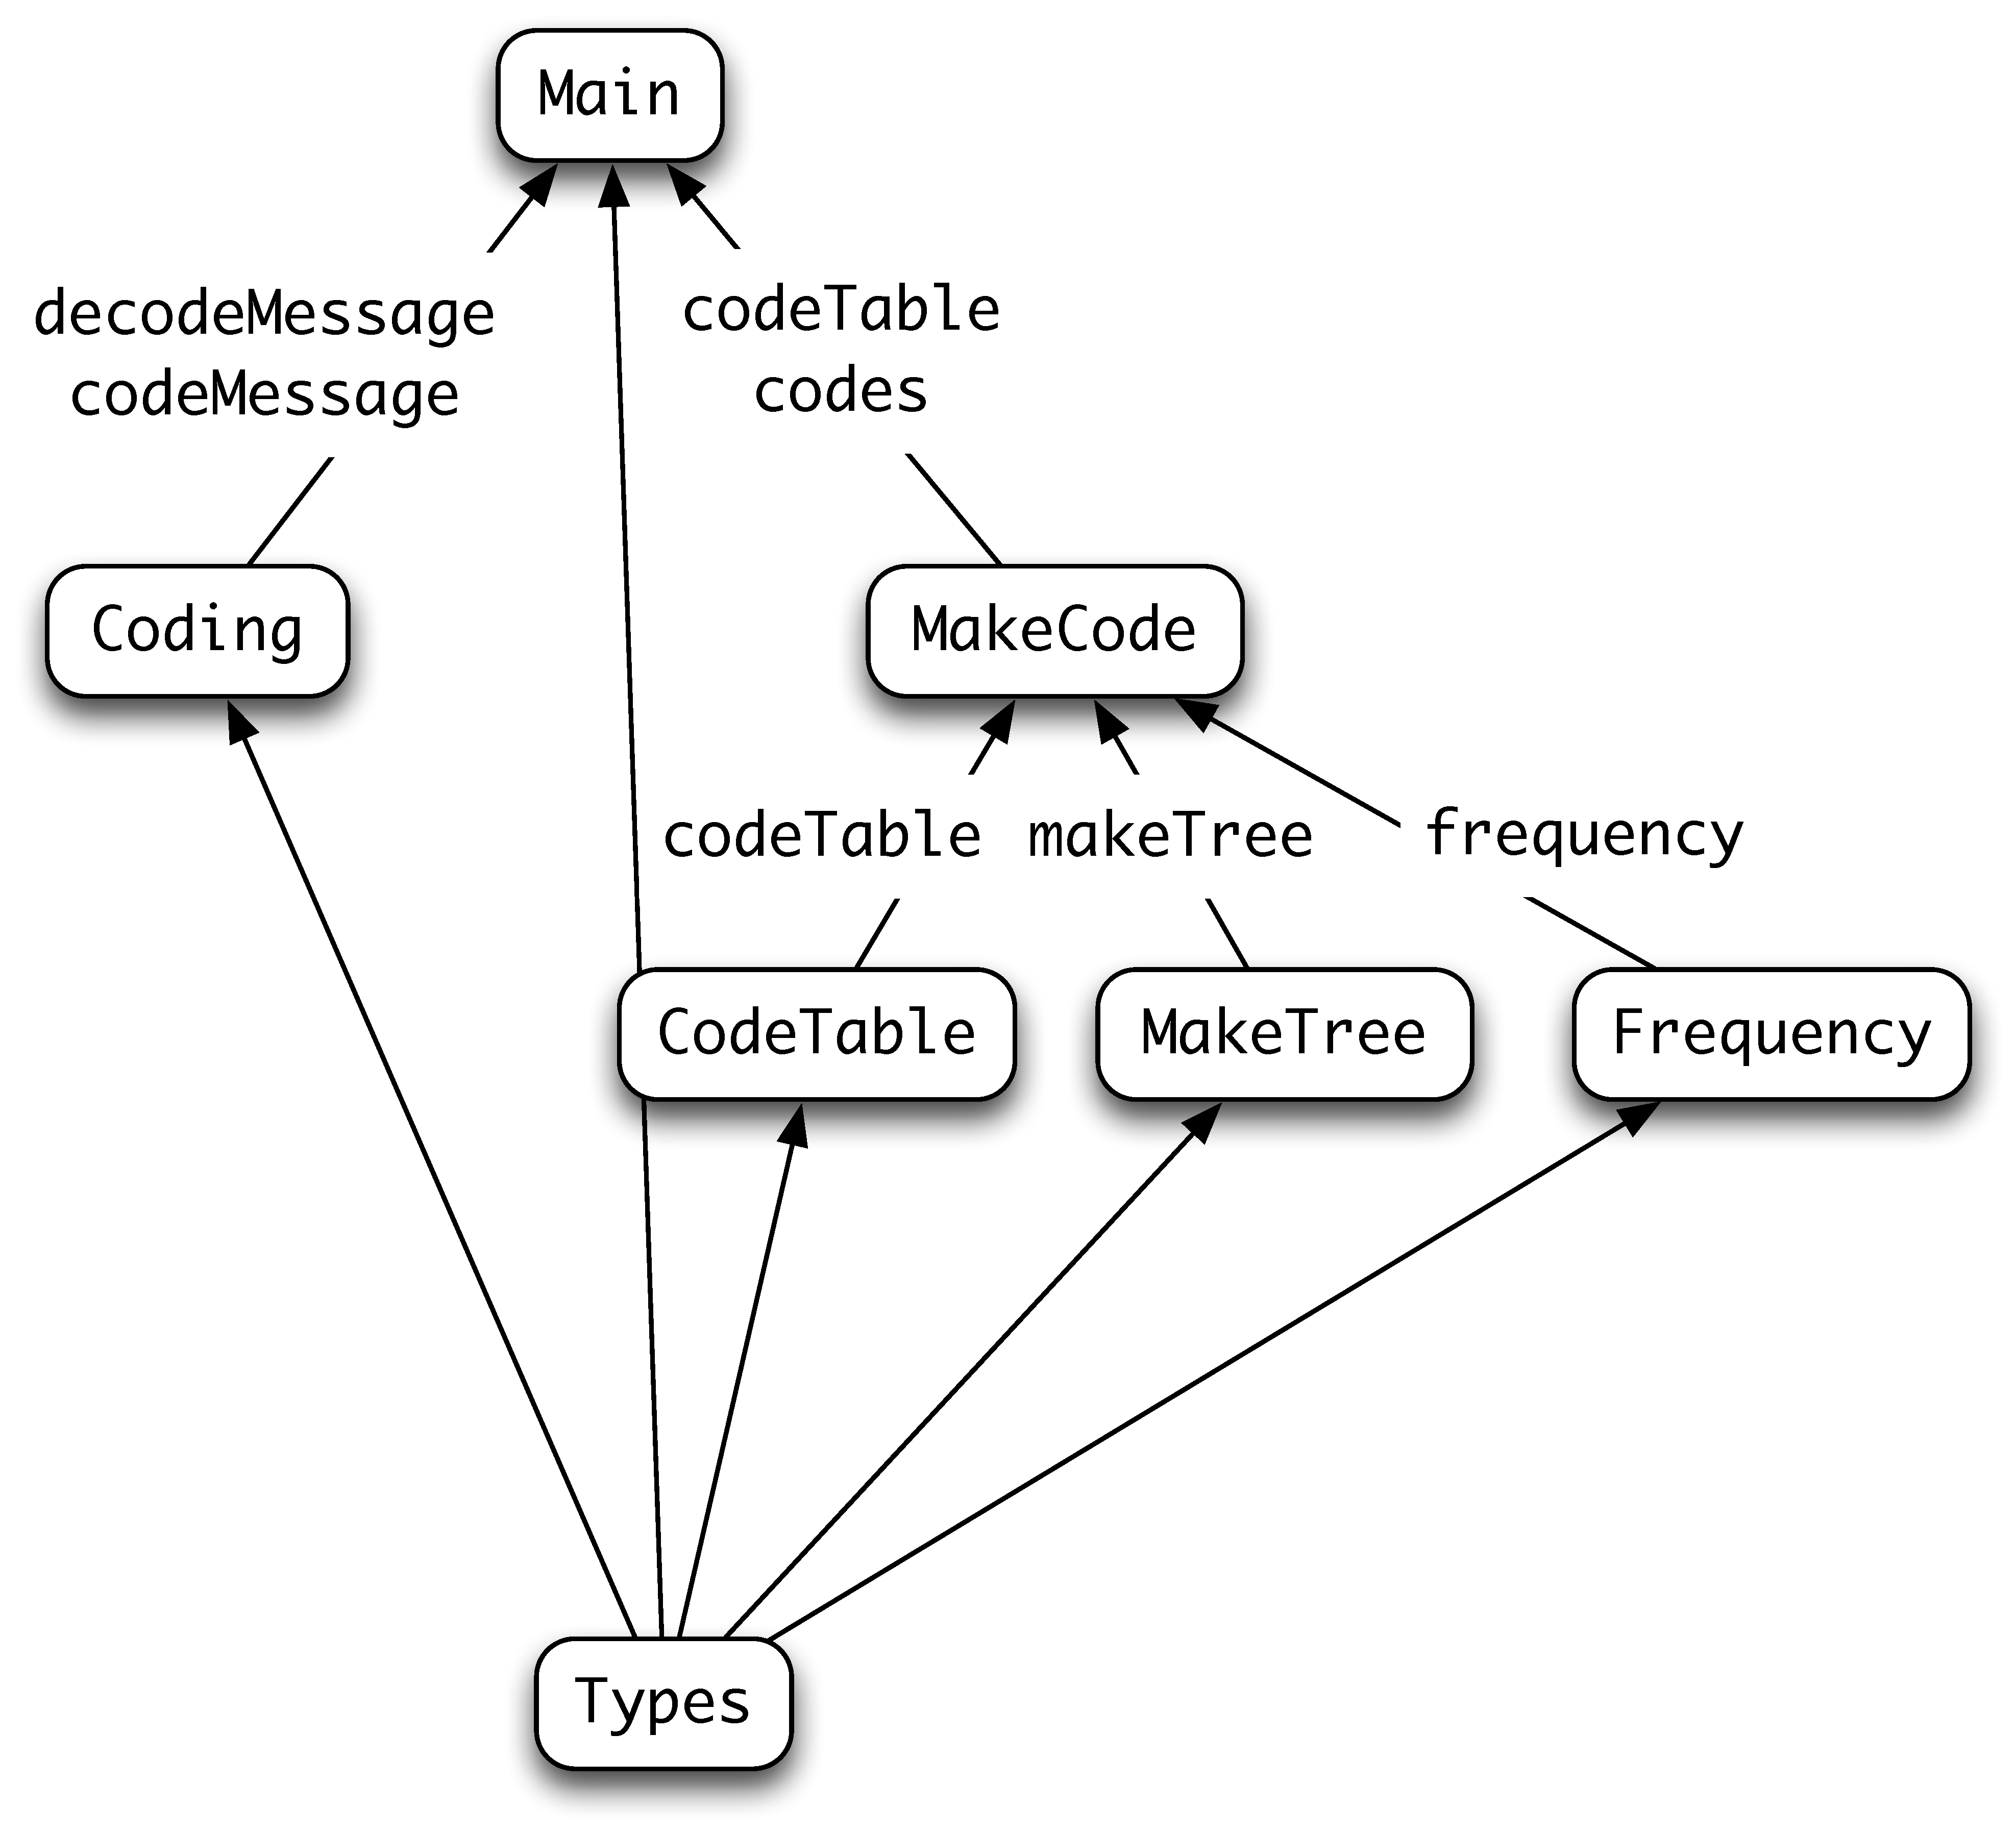
\includegraphics[width=4in]{Pictures/modules.pdf}
\end{center}
\caption{The modules of the Huffman coding system.}
\label{overallMod}
\index{modules!structure diagram}
\end{figure}



\subsection*{The top-level file -- \texttt{Main.hs}}
\minx{Main.hs}

We can now pull all the parts of the system together into a top-level file.
\begin{alltt}
module Main (main) where

import Types    ( Tree(Leaf,Node), Bit(L,R), HCode , Table )
import Coding   ( codeMessage , decodeMessage )
import MakeCode ( codes, codeTable )
\end{alltt}
In this file we can include representative examples, using the major
functions listed in the \texttt{import} statements; the code is illustrated in Figure \ref{mainMod}. 

The
structure of the system is given in Figure \ref{overallMod}. Modules are
represented by boxes, and an arrow from \texttt{A} to \texttt{B} indicates that
\texttt{A.hs} is imported into \texttt{B.hs}. An arrow is marked to indicate the
functions exported by the included module, so that, for example, \texttt{codes}
and \texttt{codeTable} are exported from \texttt{MakeCode.hs} to \texttt{Main.hs}.


If this
coding system were to be used as a component of a larger system, a 
\texttt{module} directive could be used to control which of the four functions and
the types are exported, after the module had been renamed.
It is important to realize that the types will need to
be exported (or be included in the file including \texttt{Main.hs})
if the functions are to be used.

\subsection*{Testing the system}

We can write a top-level test for a system like this, by taking an example string, coding it and then decoding it. This should take us back to the string we started with, and indeed we can see this in the particular example in Figure \ref{mainMod}. It is possible to change this to a QuickCheck property, which checks that coding/decoding is the identity for a whole collection of strings; we leave this as an exercise for the reader.\index{QuickCheck!Huffman codes}

The top-level test corresponds to a \emph{system} test, in that it uses all the functions defined -- implicitly or explicitly -- and checks the overall functionality of the system. It is also possible to write \emph{unit} tests, which check that a particular function or module has the required functionality.

For example, we might look at the module \texttt{Frequency.hs}, and in particular at the functions designed to merge or sort their arguments. A QuickCheck property embodying a unit test for these would include
\begin{alltt}\minx{prop\_mergeSort}
prop_mergeSort :: [Int] -> Bool

prop_mergeSort xs =
    sorted (mergeSort merge xs) 
\end{alltt}
where \texttt{sorted} expresses that its argument is sorted into ascending order and \texttt{merge} will merge two ordered lists in order.



\begin{exercises}

\item
Give a definition of merge sort which uses the built-in ordering `\texttt{<=}'.
What is its type?

\item
Modifying your previous answer if necessary, give a version of merge sort
which removes duplicate entries.

\item
Give a version of merge sort which takes an ordering function as a parameter:
\begin{alltt}
ordering :: a -> a -> Ordering
\end{alltt}
Explain how to implement \texttt{mergeSort freqMerge} using this version of
merge sort, and discuss why you {\em cannot\/} implement \texttt{mergeSort
alphaMerge} this way.

\item
Define the \texttt{insTree} function, used in the definition of \texttt{makeTree}.

\item
Give a calculation of
\begin{alltt}
makeTree  [('b',2),('a',2),('t',3),('e',4)]
\end{alltt}

\item
Define functions
\begin{alltt}
showTree  :: Tree  -> String
showTable :: Table -> String
\end{alltt}
which give printable versions of Huffman trees and code tables. One general
way of printing trees is to use indentation to indicate the structure.
Schematically, this looks like
\begin{alltt}
    left sub tree,  indented by 4 characters
value(s) at Node
    right sub tree, indented by 4 characters
\end{alltt}



\item
Define a QuickCheck property to test coding and decoding: specifically this should code a string and decode it, and compare the result with the original. You may need to restrict the strings over which the test is made.

\item
Define  \texttt{sorted} so that it checks whether its argument is sorted into ascending order and define \texttt{merge} which will merge two ordered lists in order. Using these check whether the property \texttt{prop\_mergeSort ::\ [Int] -> Bool}, defined earlier, holds.

\item
Write QuickCheck unit tests for other functions in \texttt{Frequency.hs} and other modules of the Hufmann coding system.

\item
You may find that it is necessary to restrict the domain over which some properties hold in order for them to QuickCheck successfully: can you re-define the functions involved so that the properties hold for \emph{all} randomly generated inputs.

\item
The correctness property for the Huffman system formulated earlier states that \texttt{decode.code} is the identity. Would you expect that \texttt{code.decode} is the identity: if so, over what domain; if not, can you give a sub-domain over which you wold expect it to hold?


\end{exercises}

\begin{summary}
When writing a program of any size, we need to divide up the work in a
sensible way. The Haskell module system allows one script to be
included in another. At the boundary, it is possible to control exactly which
definitions are exported from one module and imported into another.

We gave a number of guidelines for the design of a program into its
constituent modules. The most important advice is to make each module perform
one clearly defined task, and for only as much information as is needed to be
exported -- the principle of \textbf{information hiding}. This principle 
is extended in the next chapter when we examine abstract
data types.

The design principles were put into practice in the Huffman coding
example. In particular, it was shown for the file \texttt{MakeCode.hs} and
its three sub-modules that design can begin with the design of modules and
their \textbf{interfaces} -- that is the definitions (and their types) which are
exported. Thus the design process starts {\em before\/} any
implementation takes place.
 

\index{Huffman codes|)}

\end{summary}


%\end{document}

%\documentclass{book}\usepackage{sjtfonts}\usepackage{includegraphics}\usepackage{alltt}\usepackage{latexsym}
%\usepackage{array}
%\begin{document}\input{defs0}%		miradefs.tex 		    June 1994

% opening and closing a quoted Miranda section

\newcommand{\mira}{\noindent\hrulefill\nopagebreak\so}
\newcommand{\arim}{\nopagebreak\st\hrulefill\\}

% backslash in the Miranda environment
% Only feasible approach is to use \verb+\+
% in line!

%\newcommand{\bs}{$\mi\backslash\!\!$}
%\newcommand{\lbs}{\mbox{\verb+\+}}

% ignoring part of the input

\newcommand{\ignore}[1]{}

% a blank line in a Miranda section

\newcommand{\bl}{\mbox{\ }}

% Signalling a diffculty.

\definecolor{light-gray}{gray}{0.95}

\newcommand{\beware}[2]
 {\medskip\noindent\colorbox{light-gray}{\parbox{\textwidth}
 {\mbox{\large\textbf{#1}} \medskip\noindent\\ #2}\medskip\noindent}}

% Subscripting in Miranda text
\newcommand{\subscr}[2]{\mbox{${\mbox{\texttt{#1}}}_{\mbox{\texttt{#2}}}$}}

%\newcommand{\subscr}[2]{\mbox{${\mbox{\mi #1}}_{\mbox{\smtt #2}}$}}
\newcommand{\aone}{\subscr{a}{1}}
\newcommand{\atwo}{\subscr{a}{2}}
\newcommand{\ak}{\subscr{a}{k}}

\newcommand{\aoneone}{\subscr{a}{1,1}}

\newcommand{\eone}{\subscr{e}{1}}
\newcommand{\etwo}{\subscr{e}{2}}
\newcommand{\ei}{\subscr{e}{i}}
\newcommand{\er}{\subscr{e}{r}}

\newcommand{\fone}{\subscr{f}{1}}
\newcommand{\fl}{\subscr{f}{l}}

\newcommand{\gone}{\subscr{g}{1}}
\newcommand{\gtwo}{\subscr{g}{2}}
\newcommand{\gi}{\subscr{g}{i}}
\newcommand{\gr}{\subscr{g}{r}}

\newcommand{\hone}{\subscr{h}{1}}
\newcommand{\hl}{\subscr{h}{l}}

\newcommand{\pone}{\subscr{p}{1}}
\newcommand{\ptwo}{\subscr{p}{2}}
\newcommand{\pk}{\subscr{p}{k}}

\newcommand{\qone}{\subscr{q}{1}}
\newcommand{\qtwo}{\subscr{q}{2}}
\newcommand{\qk}{\subscr{q}{k}}

\newcommand{\rone}{\subscr{r}{1}}
\newcommand{\rtwo}{\subscr{r}{2}}

\newcommand{\tone}{\subscr{t}{1}}
\newcommand{\ttwo}{\subscr{t}{2}}
\newcommand{\tn}{\subscr{t}{n}}

\newcommand{\vone}{\subscr{v}{1}}
\newcommand{\vtwo}{\subscr{v}{2}}
\newcommand{\vn}{\subscr{v}{n}}

% for regular expressions

\newcommand{\stone}{\subscr{st}{1}}
\newcommand{\sttwo}{\subscr{st}{2}}
\newcommand{\stn}{\subscr{st}{n}}
\newcommand{\rthree}{\subscr{r}{3}}

\newcommand{\eps}{$\varepsilon$}
\newcommand{\trans}[1]{\stackrel{\mbox{\tt #1}}{\longrightarrow}}



% superscript in Miranda text

\newcommand{\superscr}[2]{\mbox{${\mbox{\mi #1}}^{\mbox{\smtt #2}}$}}

% Not equals in Miranda text

\newcommand{\noteq}{\makebox[0pt][l]{=}/}
\newcommand{\overslash}{\makebox[0pt][l]{/}}

% Definitions in complexity chapter

\newfont{\oldSym}{cmsy10}
\newcommand{\Th}{\boldmath$\oldSym\Theta$}
\newcommand{\pow}[1]{\^{}#1}
\newcommand{\leqq}{$\leq$}
\newcommand{\geqq}{$\geq$}
\newcommand{\lll}{$\ll$}
\newcommand{\eqq}{$\equiv$}
\newcommand{\ltwo}{\subscr{log}{2}}

% Indexing

\newcommand{\minx}[1]{\index{#1@{\ttfamily{}#1}}}
\setcounter{chapter}{15}\setcounter{page}{287}

\chapter{Abstract data types}
\chapstart
\label{adt}
\index{abstract data type|(}
\index{abstract data type!sets|see{sets}}
\index{abstract data type!store|see{store}}

The Haskell module system allows definitions of functions and other objects to
be hidden when one module is imported into another. Those definitions
hidden are only of use in defining the exported functions, and hiding them
makes clearer the exact interface between the two modules: only those features
of the module which are needed will be visible.

This chapter shows that information hiding is equally applicable for types,
giving what are known as \textbf{abstract data types}, or \textbf{ADT}s. We explain the abstract data type 
mechanism here, as well as
providing a number of examples of ADTs, including queues, sets, relations and the fundamental
types belonging to a simulation case study.
\minx{module}\minx{type}

\section{Type representations}

We begin our discussion with a scenario which is intended to show both the
purpose and the operation of the abstract data type mechanism.

Suppose we are to build a calculator for numerical expressions, like those
given by the \texttt{Expr}\minx{Expr} type of Section \ref{recTypes}, but with variables
included.
The calculator is to provide the facility to set the values of variables, as
well as for variables to form parts of expressions. 

As a part of our system, we need to
be able to model the current values of the variables, which we might call the
\textbf{store} of the calculator. How can this be done? A number of models
present themselves, including:\index{store}\index{case
studies!calculator|see{calculator}}\index{calculator|(}
\begin{titemize}
\item a list of integer/variable pairs: \texttt{[(Integer,Var)]}; and
\item a function from variables to integers: \texttt{(Var -> Integer)}.
\end{titemize}
Both models allow us to look up and update the values of variables, as well
as set a starting value for the store. These operations have types as
follows. 
\begin{alltt}\minx{initial}\minx{value}\minx{update}
initial :: Store
value   :: Store -> Var -> Integer  \hfill(StoreSig)\minx{Store}
update  :: Store -> Var -> Integer -> Store
\end{alltt}
but each model
allows more than that: we can, for instance, reverse a list, or compose a
function with others. In using the type \texttt{Store} we intend
only to use the three operations given, but it is always possible to use the
model in unintended ways.

How can we give a better model of a store? The answer is to define a
type which \textbf{only} has the operations \texttt{initial}, \texttt{value} and
\texttt{update}, so that we cannot abuse the representation. We
therefore hide the information about how the type is actually
implemented, and only allow the operations \texttt{(StoreSig)} to manipulate objects
of the type. 

When we provide a limited interface to a type by means of a specified set
of operations we call the type an \textbf{abstract data type} (or ADT).
\index{ADT|see{abstract data type}} 
Since the
`concrete' type itself is no longer accessible and we
may only access the type by
means of the operations provided, these operations give a more `abstract'
view of the type.

\begin{figure}[t]
\begin{center}
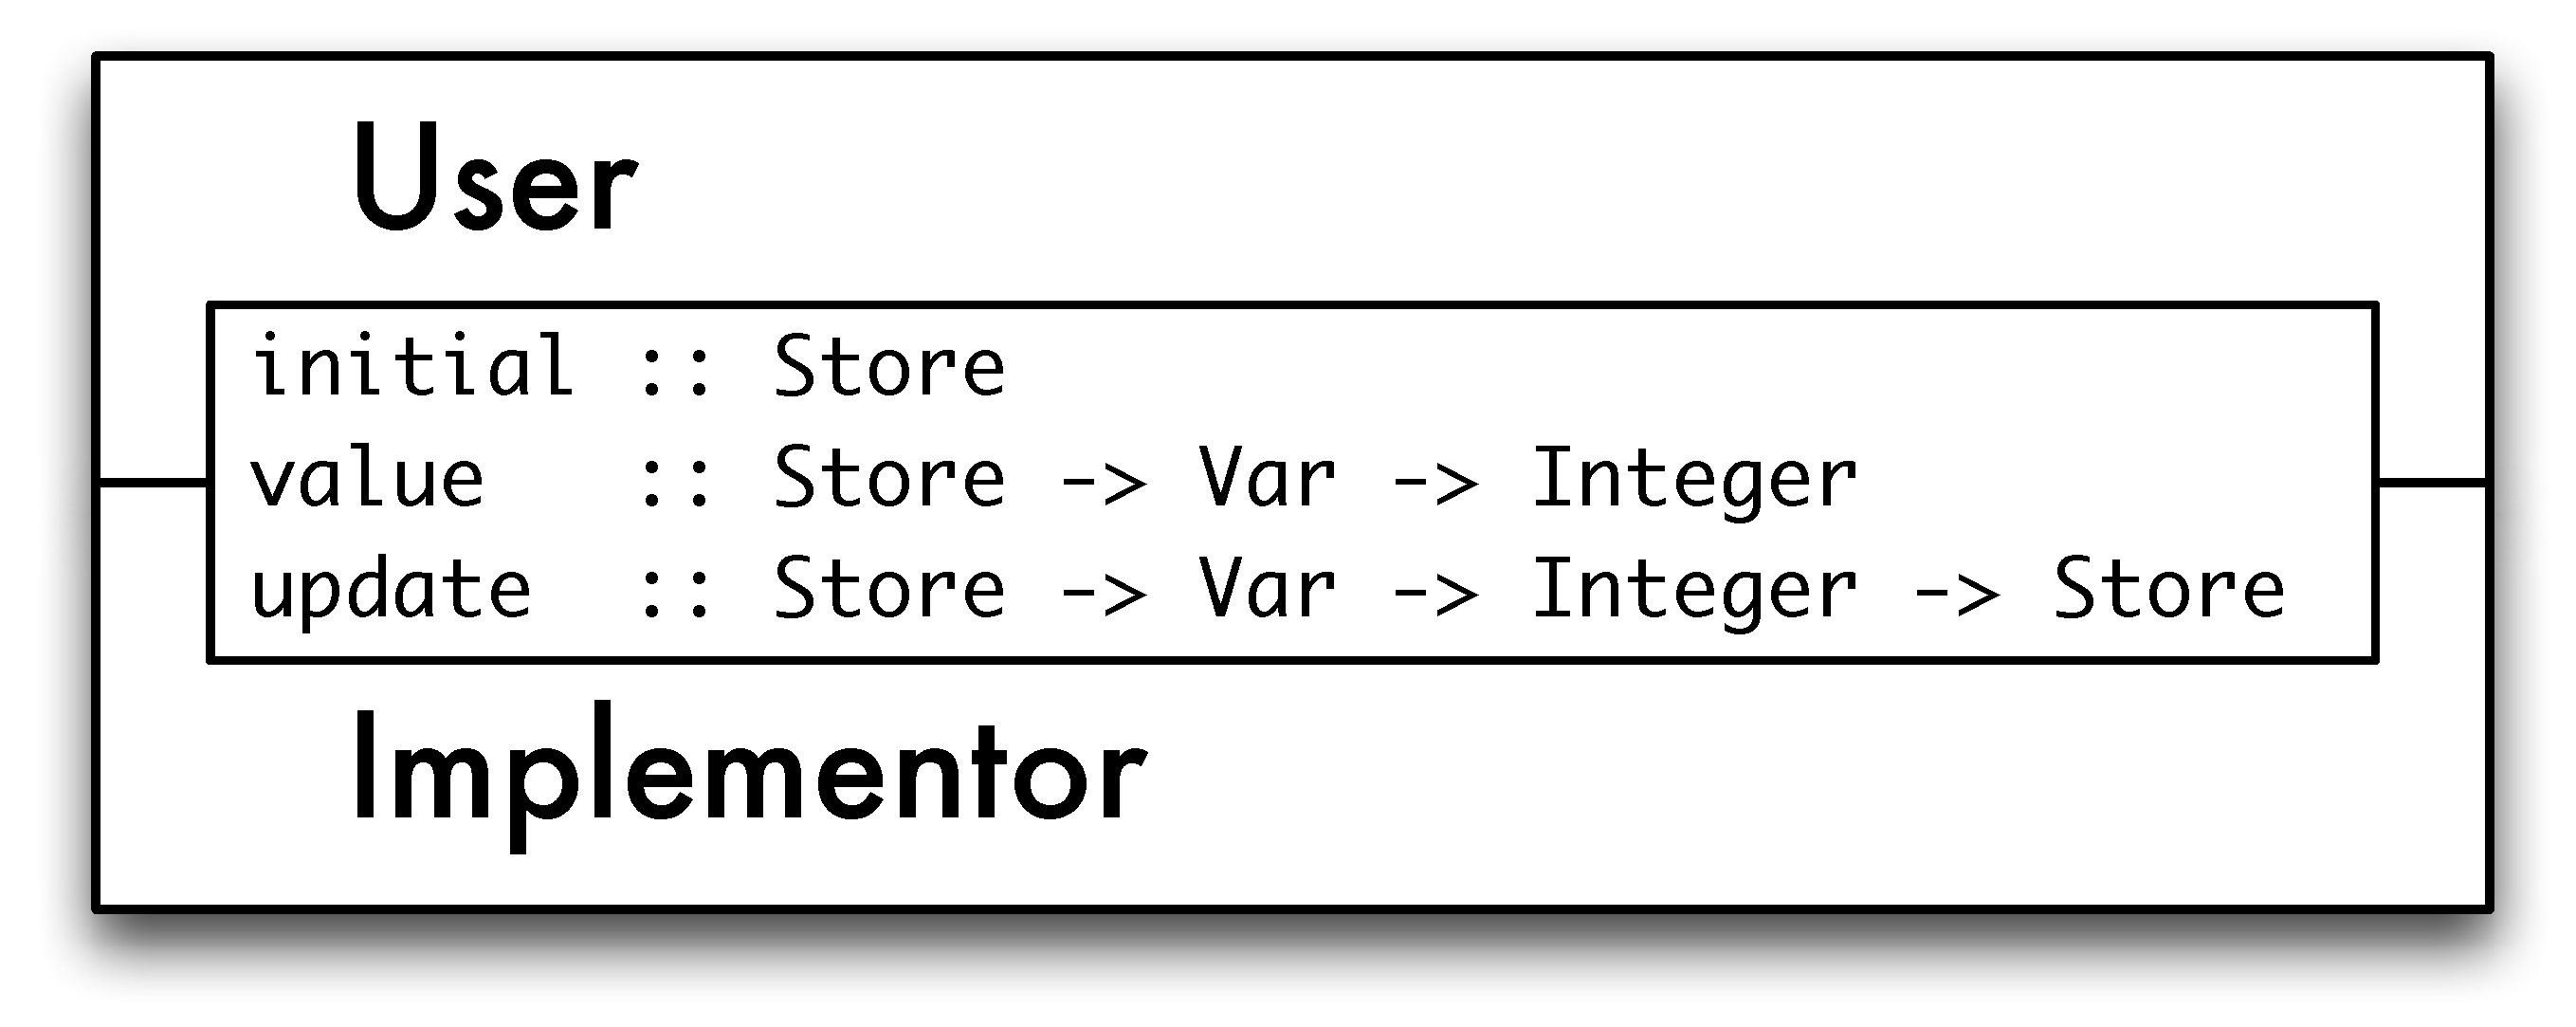
\includegraphics[width=3.5in]{Pictures/StoreADT.pdf}
\end{center}
\caption{The \texttt{Store} abstract data type.}
\label{storePic}
\end{figure}
Figure \ref{storePic} illustrates the situation, and suggests that as
well as giving a natural representation of the type of stores, there are
two other benefits of type abstraction.
\begin{titemize}
\item The type declarations in \texttt{(StoreSig)} form a clearly defined {\bf
interface},
\index{interface}
which is called the {\bf
signature}\index{signature}\index{abstract data type!signature} of the ADT, 
between the user of the type and its implementer. The only information that
they have to agree on is the signature; once this is agreed, they can work
independently. This is therefore another way of breaking a complex problem
into simpler parts; another aspect of the
`divide and conquer' method. \index{divide and conquer}
\item We can \textbf{modify} \index{program modification}the implementation of the \texttt{Store} without
having any effect on the user. Contrast this with the situation
where the implementation is visible to the user. In particular, if the
implementation is an algebraic type\index{algebraic type!vs ADT} then
any change in the implementation will mean that all
definitions that use pattern matching will have to be changed. These
will include not just those in the signature, but also any user-defined
functions which use pattern matching.
\end{titemize} 
We shall see both
aspects illustrated in the sections to come; first we look at the
details of the Haskell abstract data type mechanism.

\section{The Haskell abstract data type mechanism}
\index{abstract data type!\texttt{Store}|(}

When we introduced the Haskell module system in Chapter \ref{codes} we
saw that there were two ways in which we could export a \texttt{data}
type, called \texttt{Data} say. If we include \texttt{Data(..)} in the export
list of the module, the type is exported with its constructors; if we
include \texttt{Data} then the constructors are {\em not\/} exported,
and so we can only operate over the type using the other operations of
the signature.\index{modules!ADT via export list}

In the case of the \texttt{Store} type, our module header would be
\begin{alltt}
module Store ( Store, initial, value, update ) where
\end{alltt}
which shows that we can access the type only through the three functions
mentioned. In this book we will adopt the convention that we will also
include as comments in the module header the types of the exported
functions, giving in the case of \texttt{Store} the following header.
\index{conventions!type comments in module headers}
\begin{alltt}
module Store \minx{module}\minx{initial}\minx{value}\minx{update}
   ( Store, 
     initial,     -- Store
     value,       -- Store -> Var -> Integer
     update       -- Store -> Var -> Integer -> Store
    ) where
\end{alltt}
Now, the module must contain a definition of the \texttt{Store} type and
the functions over it. 

If the implementation type was a \texttt{data} type, then this would
complete the realization of the abstract data type. However, in our running example of
stores, we
suggested earlier that we would use a list of
pairs, \texttt{[ (Integer,Var) ]}, to model the type, and so we will have to 
define a new
\texttt{data} type, called \texttt{Store}
\begin{alltt}
data Store = Store [ (Integer,Var) ] 
\end{alltt}
which has a single constructor which we also call \texttt{Store}. This
is the function which converts a list into an element of the
\texttt{Store} type; we can think of it as `wrapping up' a list to make
it into a \texttt{Store}.\index{abstract data type!`wrapping up'
representation}

We now have to define the functions \texttt{initial}, \texttt{value} and
\texttt{update} over the \texttt{Store} type. One approach is to define
the analogous functions over \texttt{[(Integer,Var)]} and then to adapt
those. We can say\index{store!as a list}
\begin{alltt}\minx{initial}\minx{value}\minx{update}
init :: [(Integer,Var)]
init = []
     
val :: [(Integer,Var)] -> Var -> Integer
val [] v        = 0
val ((n,w):sto) v 
  | v==w        = n
  | otherwise   = val sto v

upd :: [(Integer,Var)] -> Var -> Integer -> [(Integer,Var)]
upd sto v n   = (n,v):sto
\end{alltt}
The initial store, \texttt{init}, is represented by an empty list; the value of \texttt{v}
is looked up by finding the first pair \texttt{(n,v)} in the list, and
the store is updated by adding a new \texttt{(Integer,Var)} at the front of
the list.

These functions then have to be converted to work over the type \texttt{Store}, so that
arguments and results are of the form \texttt{Store xs}
with \texttt{xs::[(Integer,Var)]}. The definitions become
\begin{alltt}\index{store!as a ADT}\minx{initial}\minx{value}\minx{update}
initial :: Store 
initial = Store []

value  :: Store -> Var -> Integer
value (Store []) v  = 0
value (Store ((n,w):sto)) v 
  | v==w            = n
  | otherwise       = value (Store sto) v

update  :: Store -> Var -> Integer -> Store
update (Store sto) v n = Store ((n,v):sto)
\end{alltt}
where we can see that the pattern of the definitions is similar, except
that we have to `unwrap' arguments of the form \texttt{(Store sto)} on
the left-hand side, and  `wrap up' results using \texttt{Store} on the
right-hand side. We look at a general mechanism for `wrapping up'
functions in the example of the \texttt{Set} ADT in Section
\ref{caseSets}.

What happens if we try to
break the abstraction barrier and deal with a \texttt{Store} as having 
the form \texttt{(Store xs)}? On typing
\begin{alltt}
initial == Store []
\end{alltt}
in a module importing \texttt{Store}
we get the type error message
\index{errors!type abstraction}\index{type error!ADT}
\begin{alltt}
Not in scope: data constructor `Store'
\end{alltt}
The fact that \texttt{initial} is indeed implemented as \texttt{Store []} is irrelevant,
since the implementation is not in scope outside the \texttt{Store} module.

\subsection*{The \texttt{newtype} construction}
\minx{newtype}

In fact in this case rather than using a \texttt{data} type we will define 
\begin{alltt}
newtype Store = Store [ (Integer,Var) ]
\end{alltt}
which has the same effect as declaring a \texttt{data} type with one unary constructor
but which is implemented in a more efficient fashion. 


\beware{Naming \texttt{newtypes}}{\index{naming \texttt{newtypes}}
Another possible way of implementing the type would be to say
\begin{alltt}
newtype Store = Sto [ (Integer,Var) ]
\end{alltt}
using different names for the type and its constructor. Although this makes it clear whether we are talking about the type or the constructor, we prefer to use a single name within this \texttt{newtype}, as otherwise we need to choose two different -- but related -- names. 

\medskip
Moreover, in practice, when we use \texttt{Store} we will always be able to tell which use -- type name or constructor -- is meant.
Finally, this convention is in widespread use in the Haskell developer community, and so it's helpful to be aware of the fact.}


\subsection*{Type classes: showing values and equality}
\index{classes!and ADTs}
\index{abstract data type!and classes}

We can declare types as belonging to particular type classes such as
\texttt{Show} and \texttt{Eq}, and this applies equally well to abstract data
types. In the case of \texttt{Store} we can say
\begin{alltt}
instance Eq Store where 
  (Store sto1) == (Store sto2) = (sto1 == sto2)					

instance Show Store where
  showsPrec n (Store sto) = showsPrec n sto		
\end{alltt}
Note, however, that once declared, these instances \textbf{cannot be
hidden}, so that even though they are not named in the export list, the
functions over \texttt{Store} which are defined by means of these
\texttt{instance} declarations will be available whenever the module
\texttt{Store} is imported. Of course, we can choose {\em not\/} to
declare these instances, and so not to provide an equality or a
\texttt{show} function over \texttt{Stores}.

\subsection*{Stores as functions}
\index{store!as function}

A different implementation of \texttt{Store} is given by the type of functions
from variables to integers. \minx{Store}
\begin{alltt}\minx{initial}\minx{value}\minx{update}
newtype Store = Store (Var -> Integer) 					

initial :: Store 
initial = Store (\bs{v} -> 0)

value :: Store -> Var -> Integer
value (Store sto) v = sto v

update  :: Store -> Var -> Integer -> Store
update (Store sto) v n 
  = Store (\bs{w} -> if v==w then n else sto w)
\end{alltt}
Under this implementation, 
\begin{itemize}
\item
the \texttt{initial} store maps every variable to
\texttt{0};
\item
to look up a \texttt{value} of a variable \texttt{v}
the store function \texttt{sto} is applied to \texttt{v}, and 
\item
in the case
of an \texttt{update}, a function returned is identical to \texttt{sto}
except on the variable whose value is changed.
\end{itemize}


\subsection*{Testing ADTs}
\index{testing!ADTs}\index{abstract data type!testing}\index{QuickCheck!testing ADTs}

Suppose that we have implemented a store as a list of integer-variable pairs. We can inspect the result of updating a store, which will be a new list, and check that it has the properties that we would expect. For example, we might take the difference of the lists before and after the update.

If we implement queues as an ADT, we \emph{can't} look directly at the underlying implementation; instead we have to write properties using the interface functions, here \texttt{initial}, \texttt{value} and \texttt{update}. We can start by saying what happens if we look up a value in the initial store:
\begin{alltt}\minx{prop\_Initial}
prop\_Initial :: Char -> Bool

prop\_Initial ch =
   value initial ch == 0
\end{alltt}
What can we say about the effect of an \texttt{update} on a store? First, if perform an update for the variable \texttt{ch} and then look up the value, we would expect to see the new value:
\begin{alltt}\minx{prop\_Update*}
prop\_Update1 :: Char -> Integer -> Store -> Bool

prop\_Update1 ch int st =
    value (update st ch int) ch == int
\end{alltt}
Finally, what if we look up the value of another variable after this update? Its value should be the same as it was before:
\begin{alltt}
prop_Update2 :: Char -> Char -> Integer -> Store -> Bool

prop_Update2 ch1 ch2 int st =
    value (update st ch2 int) ch1 == value st ch1
\end{alltt}
If we perform a QuickCheck on these properties -- the appropriate QuickCheck magic is given in the module \texttt{StoreTest} and the properties in \texttt{QCStoreTest} -- the first two pass every time, but the third one sometimes fails: that is when \texttt{ch1} and \texttt{ch2} are equal! 

Modifying the test to take this into account, we get a test that always passes:
\begin{alltt}
prop_Update2 :: Char -> Char -> Integer -> Store -> Bool

prop_Update2 ch1 ch2 int st =
    value (update st ch2 int) ch1 == value st ch1 || ch1==ch2
\end{alltt}
Because the tests are written in terms of the interface only, if we were to change the implementation then the tests could still be applied, assuming that we have the right QuickCheck definitions in place.


\begin{exercises}

\item
Give an implementation of \texttt{Store} using lists whose entries are ordered
according to the variable names. Discuss why this might be preferable to the
original list implementation, and also its disadvantages, if any.

\item 
For the implementation of \texttt{Store} as a list type \texttt{[(Integer,Var)]}, give a
definition of equality which equates any two stores which give the same values
to each variable. Can this operation be defined for the second implementation?
If not, give a modification of the implementation which allows it to be
defined.

\item
In this question you should use the type \texttt{Maybe a}.
Suppose it is an error to look up the \texttt{value}
of a variable which does not have a value in the given store. Explain how you
would modify both the signature of \texttt{Store} and the two implementations.

\item
Rather than giving an error when looking up a variable which does not have a
value in the particular store, extend the signature to provide a test of
whether a variable has a value in a given store, and explain how  would
modify the two implementations to define the test.

\item
Suppose you are to implement a fourth operation over \texttt{Store}
\begin{alltt}
setAll :: Integer -> Store
\end{alltt}
so that \texttt{setAll n} is the store where every variable has the value 
\texttt{n}. Can you do this for both the example implementations? Show how if you
can, and explain why, if not.

\item 
Design an ADT for the library database, first examined in
Chapter \ref{tupleList}.
\index{abstract data type!\texttt{Store}|)}
\index{calculator|)}
\end{exercises}


\section{Queues}
\index{abstract data type!queue|(}

A queue is a `first in, first out' structure. If first \texttt{Flo} and
then \texttt{Eddie} joins an initially\index{Flo}\index{Eddie}
empty queue, the first person to leave will be 
\texttt{Flo}. As an abstract data type, we expect to be able to add items and remove
items as well as there being an empty queue.
\begin{alltt}
module Queue \minx{Queue}\minx{emptyQ}\minx{isEmptyQ}\minx{addQ}\minx{remQ}
  ( Queue , 
    emptyQ ,       --  Queue a
    isEmptyQ ,     --  Queue a -> Bool 
    addQ ,         --  a -> Queue a -> Queue a
    remQ           --  Queue a -> (  a , Queue a )
   ) where 
\end{alltt}
The function \texttt{remQ} returns a pair -- the item removed together with the
part of the queue that remains -- if there are any items in the queue. If not,
the standard function \texttt{error} is called.

A list can be used to model a queue: we add to the end of the list, and
remove from the front, giving
\begin{alltt}\index{abstract data type!queue!as list}
newtype Queue a = Queue [a]
 
emptyQ :: Queue a
emptyQ = Queue []

isEmptyQ :: Queue a -> Bool
isEmptyQ (Queue []) = True
isEmptyQ _          = False

addQ   :: a -> Queue a -> Queue a
addQ x (Queue xs) = Queue (xs++[x])

remQ   :: Queue a -> (  a , Queue a )
remQ q@(Queue xs)
  | not (isEmptyQ q)   = (head xs , Queue (tail xs))
  | otherwise          = error "remQ"
\end{alltt}


\beware{As (\texttt{@}) patterns}{
The definition of \texttt{remQ} uses an aspect of pattern matching which
we have not seen so far. We use the pattern \texttt{q@(Queue xs)}, where we can read
`\texttt{@}' as `as', to match\index{pattern matching!\texttt{"@}: `as'
pattern}\index{"@@\texttt{"@}}
the input. The variable \texttt{q} matches the whole
input, while it is also matched against \texttt{Queue xs}, so that
\texttt{xs} gives us access to the list from which it is built. This
means that we can refer directly to the whole input {\em and\/} to its
components in the definition. Without this, the alternative would be
\begin{alltt}
remQ (Queue xs)

\ \ | not (isEmptyQ (Queue xs)) = (head xs , Queue (tail xs))
  
\ \ | otherwise\ \ \ \ \ \ \ \ \ \ \ \ \ \ \ \ \ = error "remQ"
\end{alltt}
in which we have to rebuild the original queue from \texttt{xs}. 
}

\medskip\noindent
In implementing queues, rather than adding elements at the end of the list, we could choose to add them at the beginning of the list.
This leaves \texttt{emptyQ} and \texttt{isEmptyQ}
unchanged, and gives
\begin{alltt}\index{abstract data type!queue!as list}
addQ x (Queue xs) = Queue (x:xs)

remQ q@(Queue xs)
  | not (isEmptyQ q)   = (last xs , Queue (init xs))
  | otherwise          = error "remQ"
\end{alltt}
where the built-in functions \texttt{last} and \texttt{init} take the last element
and the remainder of a list.

Although we have not said exactly how to calculate the cost of evaluation (a
topic we take up in Chapter \ref{behaviour}), we can see that in each
implementation one of the operations is `cheap'  and the other is `expensive'.
The `cheap'  functions -- \texttt{remQ} in the first implementation and 
\texttt{addQ} in the second -- can be
evaluated in one step, while in both cases the `expensive' function will have
to run along a list \texttt{xs} one step per element, and so will be
costly if the list is long.

Is there any way of making both operations `cheap'? The idea is to make the
queue out of {\em two\/} lists, so that both adding and removing an element
can take place at the head of a list. The process is illustrated in Figure
\ref{twoListQ},
\begin{figure}[t]
\begin{alltt}
\end{alltt}
\begin{center}
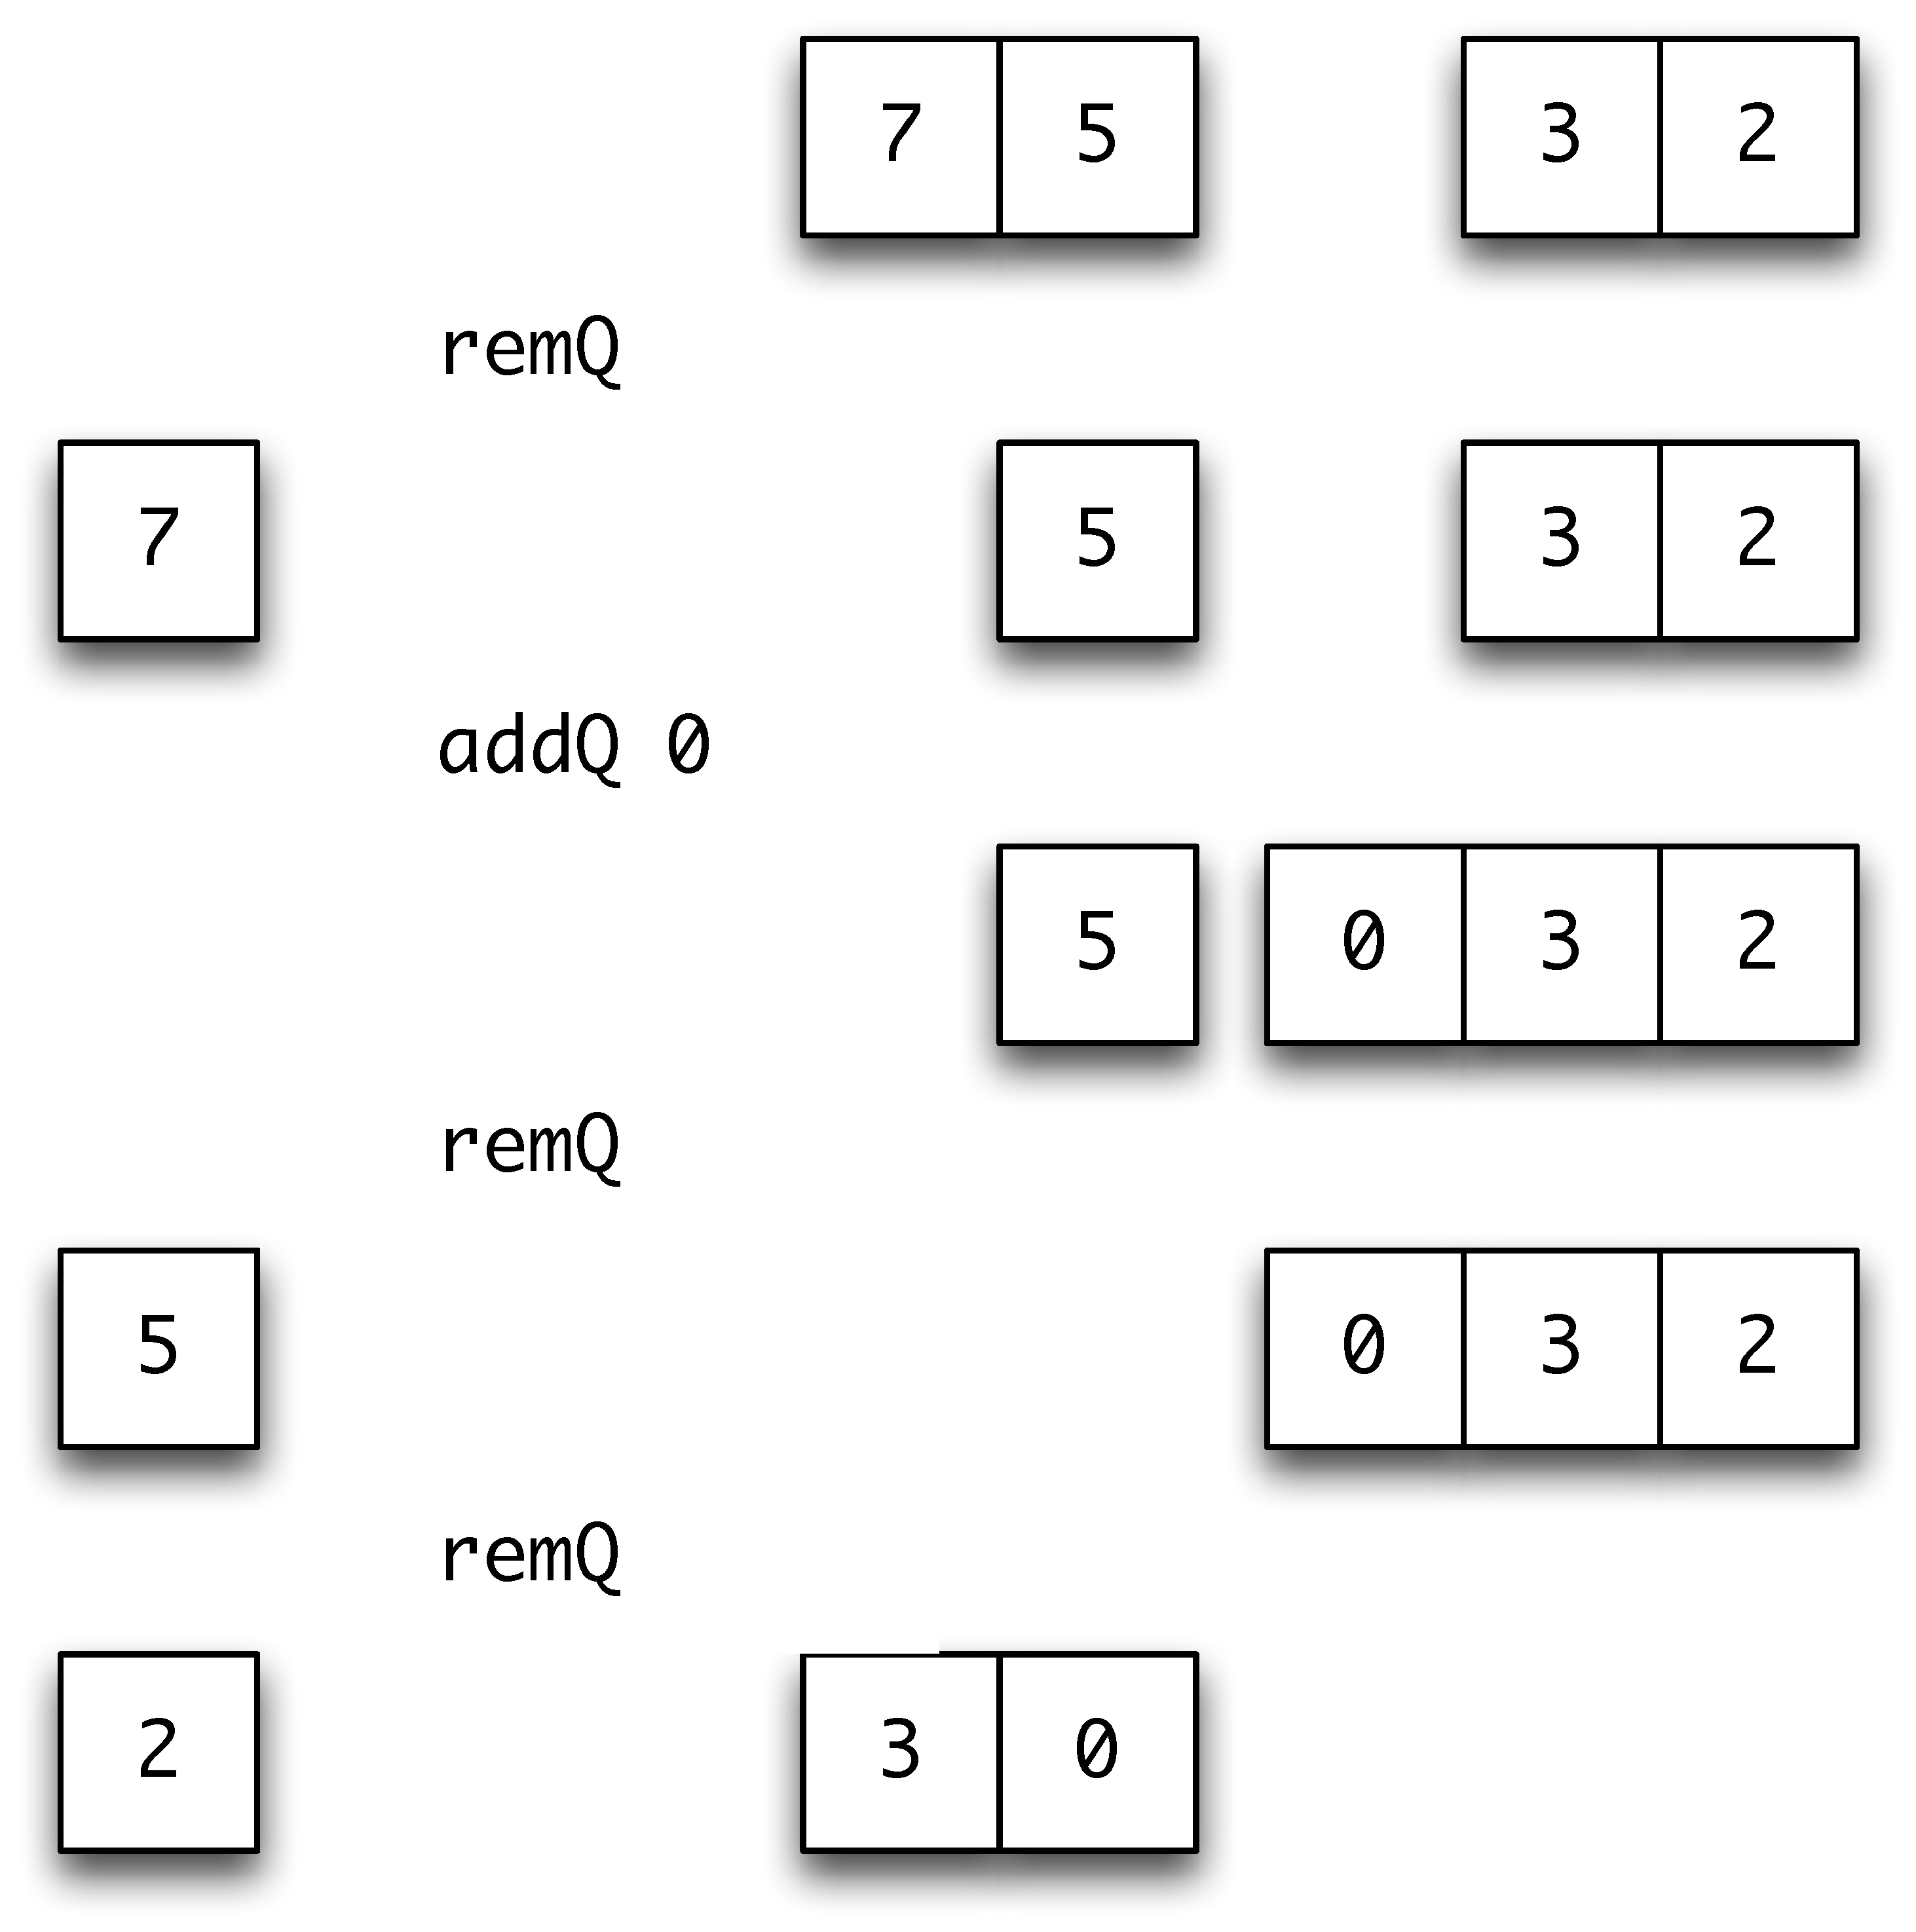
\includegraphics[width=3in]{Pictures/TwoListQueue.pdf}
\end{center}
\begin{alltt}
\end{alltt}
\caption{A two-list queue in action.}
\label{twoListQ}
\end{figure}\index{abstract data type!queue!as two lists}
which represents a number of queues. Initially the queue containing the elements
\texttt{7}, \texttt{5}, \texttt{2} and \texttt{3} is shown: here \texttt{7} is the oldest element in the queue and \texttt{3} the most recent addition. Subsequently
we see the effect of
removing an element, adding the element \texttt{0}, and removing two further
elements. In each case the queue is represented by two lists, each being shown with its head at the left-hand side.

The function \texttt{remQ} removes elements from the head of the left-hand list,
and \texttt{addQ} adds elements to the head of the right. This works until the
left-hand list is empty, when the elements of the right-hand queue have to be
transferred to the
left, reversing their order.  

This case in which we have to transfer elements is expensive, as we have to run
along a list to reverse it,
but we would not in general expect to perform this every
time we remove an element from the queue.
The Haskell implementation follows now.
\begin{alltt}
data Queue a = Queue [a] [a]

emptyQ :: Queue a
emptyQ = Queue [] []

isEmptyQ :: Queue a -> Bool
isEmptyQ (Queue [] []) = True
isEmptyQ _             = False

addQ   :: a -> Queue a -> Queue a
addQ x (Queue xs ys) = Queue xs (x:ys)

remQ   :: Queue a -> (  a , Queue a )
remQ (Queue (x:xs) ys)    = (x , Queue xs ys)
remQ (Queue [] ys@(z:zs)) = remQ (Queue (reverse ys) [])
remQ (Queue [] [])        = error "remQ"
\end{alltt}
As we commented for the \texttt{Store} types, the behaviour of this implementation
will be indistinguishable from the first two, as far as the operations of the
abstract data type
are concerned. On the other hand, the implementation will be
substantially more efficient than the single list implementations, as we
explained above. A thorough examination of recent work on the efficient implementation
of data structures in functional languages  can be found in \citeN{okasakiBook}.
\index{abstract data type!queue|)}

\beware{Using \texttt{newtype}}{
Why didn't we use a \texttt{newtype} in the definition of \texttt{Queue}? The reason is that a  \texttt{newtype} must have a single argument, and \texttt{Queue} has two; we could pair the arguments, and then use a \texttt{newtype}. We leave this as an exercise for the reader.}

\begin{exercises}

\item
Give calculations of
\begin{alltt}
"abcde" ++ "f"
init "abcdef"
last "abcdef"
\end{alltt}
where
\begin{alltt}
init x = take (length x-1) x
last x = x !! (length x-1)
\end{alltt}

\item
Explain the behaviour of the three queue models if you are asked to
perform the following sequence of queue operations: 
add 2,
add 1,
remove item,
add 3,
remove item,
add 1,
add 4,
remove item,
remove item.


\item
Define QuickCheck properties which will test the queue implementations given here. We will show how to define the appropriate generators needed to perform the tests in Chapter \ref{dsls}.


\item
A double-ended queue, or deque, allows elements to be added or removed from
either end of the structure. Give a signature for the ADT \texttt{Deque a},
and give two different implementations of the deque type.

\item
A unique queue can contain only one occurrence of each entry (the one to
arrive earliest). Give a signature for the ADT of these queues, and an
implementation of the ADT.

\item
Each element of a priority queue has a numerical priority. When an element is
removed, it will be of the highest priority in the queue. If there is more
than one of these, the earliest to arrive is chosen. Give a signature and
implementation of the ADT of priority queues. 

\item
{[Harder]}
Examine how priority queues could be used to implement the Huffman coding
system in Chapter \ref{codes}.
\end{exercises}

\section{Design}
\label{adtDesign}
\index{design!abstract data types|(}

This section examines the design of Haskell abstract data types, and how the
presence of this mechanism affects design in general.

\subsection*{General principles}

In building a system, the choice of types is fundamental, and affects the
subsequent design and implementation profoundly. If we use abstract data
types at an early stage we hope to find `natural' representations of the
types occurring in the problem. Designing the abstract data types is a three-stage process.  
\begin{titemize}
\item First we need
to identify and \textbf{name} the types in the system.
\item Next, we should give
an \textbf{informal description} of what is expected from each type. 
\item Using this
description we can then move to writing the \textbf{signature}\index{signature} of each 
abstract data type.
\end{titemize}
How do we decide what should go in the signature? This is the \$64,000
question, of course, but there are some general questions we can ask of any
abstract data type signature.
\begin{titemize}
\item Can we create objects of the type? For instance, in the \texttt{Queue a}
type, we have the object \texttt{emptyQ}, and in a type of sets, we might give a
function taking an element to the `singleton' set containing that element
alone. If there are no such objects or functions, something is wrong!
\item Can we check what sort of object we have? In a tree ADT we might
want to check whether we have a leaf or a node, for instance.
\item Can we extract the components of objects, if we so require? Can we take
the head of a \texttt{Queue a}, say?
\item Can we transform objects: can we reverse a list, perhaps, or add an
item to a queue? 
\item Can we combine objects? We might want to be able to join
together two trees, for example.
\item Can we collapse objects? Can we take the sum of a numerical list, or
find the size of an object, say? 
\end{titemize}
Not all these questions are appropriate in every case, but the majority of
operations we perform on types fall into one of these categories. All the
operations in the following signature for binary trees can be so classified,
for instance.
\begin{alltt}
module Tree\minx{Tree}\index{signature!for \texttt{Tree}}
  (Tree,
   nil,           -- Tree a
   isNil,         -- Tree a -> Bool  
   isNode,        -- Tree a -> Bool
   leftSub,       -- Tree a -> Tree a 
   rightSub,      -- Tree a -> Tree a 
   treeVal,       -- Tree a -> a
   insTree,       -- Ord a => a -> Tree a -> Tree a 
   delete,        -- Ord a => a -> Tree a -> Tree a
   minTree        -- Ord a => Tree a -> Maybe a
  ) where
\end{alltt}
Other functions might be included in the signature; in the case of \texttt{Tree
a} we might want to include the \texttt{size}
function. This function can be defined
using the other operations.
\begin{alltt}
size :: Tree a -> Integer\minx{size}
size t 
  | isNil t     = 0
  | otherwise   = 1 + size (leftSub t) + size (rightSub t)
\end{alltt}
This definition of \texttt{size} is \textbf{independent} of the implementation,
and so would not have to be reimplemented if the implementation type for
\texttt{Tree a} changed. This is a good reason for leaving \texttt{size} out
of the signature, and this is a check we can make for any signature: are all
the functions in the signature needed? We come back to this point, and the
tree type, later in the chapter. Now we look at a larger-scale example.

\begin{exercises}

\item
Are all the operations in the \texttt{Tree a} signature necessary? Identify those
which can be implemented using the other operations of the signature.

\item
Design a signature for an abstract type of library databases, as first
introduced in Chapter \ref{tupleList}.

\item
Design a signature for an abstract type of indexes, as examined in Section
\ref{indexExam}. 

\index{abstract data type|)}
\index{design!abstract data types|)}
\end{exercises}
\section{Simulation}
\index{simulation|(}

\label{simEx}

We first introduced the simulation example in Section \ref{algDesign}, where
we designed the algebraic types \texttt{Inmess} and \texttt{Outmess}. Let us
suppose, for ease of exposition, that the system time is measured in minutes.

The \minx{Inmess}\minx{Outmess}
\texttt{Inmess} \texttt{No} signals no arrival, while \texttt{Yes 34 12} signals the
arrival of a customer at the \texttt{34}th minute, who will need \texttt{12} minutes
to be served. 

The \texttt{Outmess} \texttt{Discharge 34 27 12} signals that the person arriving
at time \texttt{34} waited \texttt{27} minutes before receiving their \texttt{12}
minutes of service.

Our aim in this section is to design the ADTs for a simple
simulation of queueing. We start by looking at a single queue. Working
through the stages, we will call the type \texttt{QueueState}, and it can be
described thus. 
\begin{quote}
There are two main operations on a queue. The first is to add a new item, an
\texttt{Inmess}, to the queue. The second is to process the queue by a one-minute
step; the effect of this is to give one minute's further processing to the
item at the head of the queue (if there is such a thing). Two outcomes are
possible: the item might have its processing completed, in which case an 
\texttt{Outmess} is generated, or further processing may be needed.

Other items we need are an empty queue, an indication of
the length of a queue and a test of whether a queue is empty.
\end{quote}
This description leads directly to a signature declaration
\begin{alltt}
module QueueState \minx{QueueState}
  ( QueueState ,
    addMessage,      -- Inmess -> QueueState -> QueueState
    queueStep,       -- QueueState -> ( QueueState , [Outmess] )
    queueStart,      -- QueueState
    queueLength,     -- QueueState -> Int
    queueEmpty       -- QueueState -> Bool
    ) where
\end{alltt}
The \texttt{queueStep} function returns a pair: the \texttt{QueueState}
after a step of
processing, and a \textbf{list} of \texttt{Outmess}. A list is used, rather
than a single \texttt{Outmess}, so that in the case of no output an empty list
can be returned.

The \texttt{QueueState} type allows us to model a situation in which all
customers are served by a single processor (or bank clerk). How can we model
the case where there is more than one queue? We call this a \textbf{server}
and it is to be modelled by the \texttt{ServerState} ADT.
\begin{quote}
A server consists of a collection of queues, which can be identified by
the integers \texttt{0}, \texttt{1} and so on. It is assumed that the system
receives one \texttt{Inmess} each minute: at most one person arrives every
minute, in other words. 
 
There are three principal operations on a server.
First, we should be able to add an \texttt{Inmess} to one of the queues.
Second, a processing step of the server is given by processing each of the
constituent queues by one step: this can generate a list of \texttt{Outmess}, as
each queue can generate such a message. Finally, a step of the simulation
combines a server step with allocation of the \texttt{Inmess} to the shortest
queue in the server.

Three other operations are necessary. We have a starting server, consisting
of the appropriate number of empty queues, and we should be able to identify
the number of queues in a server, as well as the shortest queue it contains.

\end{quote}
\vspace{5pt}

As a signature, we have
\begin{alltt}
module ServerState \minx{ServerState}
  ( ServerState ,
    addToQueue,     -- Int -> Inmess -> ServerState -> ServerState
    serverStep,     -- ServerState -> ( ServerState , [Outmess] )
    simulationStep, -- ServerState -> Inmess -> ( ServerState , 
                                                  [Outmess] ) 
    serverStart,    -- ServerState
    serverSize,     -- ServerState -> Int
    shortestQueue   -- ServerState -> Int
  ) where
\end{alltt}
In the next section we explore how to implement these two abstract data types.
It is important to realize that users of the ADTs can begin to do their
programming now: all the information that they need to know is contained
in the signature of the abstract data type.\looseness=-1

\begin{exercises}
\item
Are there redundant operations in the signatures of the ADTs 
\texttt{QueueState} and \texttt{ServerState}?

\item
Design a signature for \textbf{round-robin} simulation,
in which allocation of the first item is to queue \texttt{0}, the second to queue
\texttt{1}, and so on, starting again at \texttt{0} after the final queue has had an 
element assigned to it. 
\end{exercises}

\section{Implementing the simulation}

This section gives an implementation of the ADTs for a queue and a
server. The \texttt{QueueState} is implemented from scratch, while the 
\texttt{ServerState} implementation builds on the \texttt{QueueState} ADT. This
means that the two implementations are independent; modifying the
implementation of \texttt{QueueState} has no effect on the implementation of
\texttt{ServerState}.
\subsection*{The queue}
\index{simulation!the queue}

In the previous section, we designed the interfaces for the ADT;
how do we proceed with implementation? First we ought to look again at the
description of the \texttt{QueueState} type. What information does this imply
the type should contain?
\begin{titemize}
\item There has to be a \textbf{queue} of \texttt{Inmess} to be processed. This
can be represented by a list, and we can take the item at the head of the
list as the item currently being processed.
\item We need to keep a record of the processing time given to the head item,
up to the particular time represented by the state.
\item In an \texttt{Outmess}, we need to give the waiting
time for the particular item being processed. We know the time of arrival
and the time needed for processing -- if we also know the current time, we
can calculate the waiting time from these three numbers.
\end{titemize} 
It therefore seems sensible to define
\begin{alltt}
data QueueState = QS Time Service [Inmess]
                  deriving (Eq, Show)\minx{QueueState}
\end{alltt}
where the first field gives the current time, the second the service time so
far for the item currently being processed,
and the third the queue itself. Now we look at the operations one by one.
To add a message, it is put at the end of the list of messages.
\begin{alltt}
addMessage  :: Inmess -> QueueState -> QueueState

addMessage im (QS time serv ml) = QS time serv (ml++[im])
\end{alltt}
The most complicated definition is of \texttt{queueStep}. As was explained
informally, there are two principal cases, when there is an item being
processed.
\begin{alltt}
queueStep   :: QueueState -> ( QueueState , [Outmess] )\minx{queueStep}

queueStep (QS time servSoFar (Yes arr serv : inRest))
  | servSoFar < serv
    = (QS (time+1) (servSoFar+1) (Yes arr serv : inRest) , [])
  | otherwise
    = (QS (time+1) 0 inRest , [Discharge arr (time-serv-arr) serv])
\end{alltt}
In the first case, when the service time so far (\texttt{servSoFar}) is smaller
than is required (\texttt{serv}), processing is not complete. We therefore add one to
the time, and the service so far, and produce no output message. 
 
If processing is complete -- which is the
\texttt{otherwise} case -- the new state of the queue is  
\texttt{QS (time+1) 0 inRest}. In this state the time is advanced by one,  
processing time is set to zero and the head item in the list is removed.
An output message is also produced in which the
waiting time is given by subtracting the service and arrival times from the
current time.

If there is nothing to process, then we simply have to advance the current
time by one, and produce no output.
\begin{alltt}
queueStep (QS time serv []) = (QS (time+1) serv [] , [])
\end{alltt}
Note that the case of an input message \texttt{No} is not handled here since these
messages
are filtered out by the server; this is discussed below.

The three other functions are given by
\begin{alltt}
queueStart  :: QueueState
queueStart  =  QS 0 0 [] 

queueLength :: QueueState -> Int
queueLength (QS _ _ q) = length q

queueEmpty  :: QueueState -> Bool
queueEmpty (QS _ _ q)  = (q==[])
\end{alltt}
and this completes the implementation.

Obviously there are different possible implementations. We might choose to
take the item being processed and hold it separately from the queue, or
to use an ADT for the queue part, rather than a `concrete' list. 

\subsection*{The server}
\index{simulation!the server}

The server consists of a collection of queues, accessed by integers from 
\texttt{0}; we choose to use a \textbf{list} of queues.
\begin{alltt}
newtype ServerState = SS [QueueState] 
                         deriving (Eq, Show)\minx{ServerState}
\end{alltt}
Note that the implementation of this ADT builds on another ADT; this
is not unusual. Now we take the functions in turn.

Adding an element to a queue uses the function \texttt{addMessage} from the 
\texttt{QueueState} abstract type.
\begin{alltt}\minx{addToQueue} 
addToQueue :: Int -> Inmess -> ServerState -> ServerState
 
addToQueue n im (SS st)
  = SS (take n st ++ [newQueueState] ++ drop (n+1) st)
    where
    newQueueState = addMessage im (st!!n)
\end{alltt}
A step of the server is given by making a step in each of the constituent
queues, and concatenating together the output messages they produce.
\begin{alltt} 
serverStep :: ServerState -> ( ServerState , [Outmess] )\minx{serverStep}

serverStep (SS [])
  = (SS [],[])
serverStep (SS (q:qs)) 
  =  (SS (q':qs') , mess++messes)
    where
    (q' , mess)       = queueStep  q
    (SS qs' , messes) = serverStep (SS qs)
\end{alltt}
In making a simulation step, we perform a server step, and then add the
incoming message, if it indicates an arrival, to the shortest queue. 
\begin{alltt}
simulationStep       \minx{simulationStep}
  :: ServerState -> Inmess -> ( ServerState , [Outmess] )

simulationStep servSt im 
  = (addNewObject im servSt1 , outmess)
    where
    (servSt1 , outmess) = serverStep servSt
\end{alltt}
Adding the message to the shortest queue is done by \texttt{addNewObject}, which
is not in the signature. The reason for this is that it can be defined using
the operations \texttt{addToQueue} and \texttt{shortestQueue}.
\begin{alltt}
addNewObject :: Inmess -> ServerState -> ServerState

addNewObject No servSt = servSt

addNewObject (Yes arr wait) servSt
  = addToQueue (shortestQueue servSt) (Yes arr wait) servSt
\end{alltt}
It is in this function that the input messages \texttt{No} are not passed to the
queues, as was mentioned above.

The other three functions of the signature are standard.
\begin{alltt}
serverStart :: ServerState
serverStart = SS (replicate numQueues queueStart) 
\end{alltt}
where \texttt{numQueues} is a constant to be defined, and the standard function
\texttt{replicate} returns a list of \texttt{n} copies of \texttt{x} when applied thus: 
\texttt{replicate n x}.
\begin{alltt} 
serverSize :: ServerState -> Int
serverSize (SS xs) = length xs
\end{alltt}
In finding the shortest queue, we use the \texttt{queueLength} function from the
\texttt{QueueState} type.
\begin{alltt}
shortestQueue :: ServerState -> Int
 
shortestQueue (SS [q]) = 0
shortestQueue (SS (q:qs)) 
  | (queueLength (qs!!short) <= queueLength q)   = short+1
  | otherwise                                    = 0
      where
      short = shortestQueue (SS qs)
\end{alltt}
This concludes the implementation of the two simulation ADTs. The example
is intended to show the merit of designing in stages. First we gave an
informal description of  the operations on the types, then a description of
their signature, and finally an implementation. Dividing the problem up in
this way makes each stage easier to solve. 

The example also shows that types
can be implemented \textbf{independently}: since \texttt{ServerState} uses only the
abstract data type operations over \texttt{QueueState}, we can reimplement  
\texttt{QueueState} without affecting the server state at all.

\begin{exercises} 

\item
Give calculations of the expressions
\begin{alltt}
queueStep (QS 12 3 [Yes 8 4])
queueStep (QS 13 4 [Yes 8 4])
queueStep (QS 14 0 [])
\end{alltt}

\item
If we let
\begin{alltt}
serverSt1 = SS [ (QS 13 4 [Yes 8 4]) , (QS 13 3 [Yes 8 4]) ]
\end{alltt}
then give calculations of 
\begin{alltt}
serverStep serverSt1
simulationStep (Yes 13 10) serverSt1
\end{alltt}


\item
Define QuickCheck properties which will test the simulation system. We will show how to define the appropriate generators needed to perform the tests in Chapter \ref{dsls}.



\item
Explain why we cannot use the function type \texttt{(Int -> QueueState)} as the
representation type of \texttt{ServerState}. Design an extension of this type
which will represent the server state, and implement the functions of the
signature over this type.

\item
Given the implementations of the ADTs from this section,
is your answer to the question of
whether there are redundant operations in the signatures of queues and servers
any different?

\item
If you have not done so already, design a signature for round-robin simulation,
in which allocation of the first item is to queue \texttt{0}, the second to queue
\texttt{1}, and so on. 

\item 
Give an implementation of the round-robin simulation which {\em uses\/} the 
\texttt{ServerState} ADT.

\item
Give a different implementation
of the round-robin simulation which {\em modifies\/}
the implementation of the type \texttt{ServerState} itself.
\end{exercises}
\index{simulation|)}


\section{Search trees}
\label{srchTrees}
\index{search tree|(}

A binary search tree is an object of type \texttt{Tree a} whose elements are
\textbf{ordered}.  A general binary tree is implemented by the algebraic
data type \texttt{Tree}:
\begin{alltt}\minx{Tree}
data Tree a = Nil | Node a (Tree a) (Tree a)
\end{alltt}
When is a tree ordered?
The tree {\mi(Node val \tone\ \ttwo)} is ordered if 
\begin{titemize}
\item all values in \texttt{\tone} are
smaller than \texttt{val},  
\item all values in \texttt{\ttwo} are larger than \texttt{val}, and
\item the trees \texttt{\tone} and \texttt{\ttwo} are themselves ordered;
\end{titemize}
and the tree \texttt{Nil} is ordered.

Search trees are used to represent sets of elements, for instance. How can we
create a type of search trees? The concrete (algebraic) type \texttt{Tree a} will not serve, as it
contains elements like \texttt{Node 2 (Node 3 Nil Nil) Nil}, which are not
ordered.

The answer is to build elements of the type \texttt{Tree a}
using only operations which create
or preserve order. We ensure that only these `approved' operations are used
by making the type an abstract data type. 

\subsection*{The abstract data type for search trees}
\index{abstract data type!search tree}

We discussed the signature of the abstract data type earlier, in Section
\ref{adtDesign}, but we repeat it here.
\begin{alltt}
module Tree\minx{Tree}\index{signature!for \texttt{Tree}}
  (Tree,
   nil,           -- Tree a
   isNil,         -- Tree a -> Bool  
   isNode,        -- Tree a -> Bool
   leftSub,       -- Tree a -> Tree a 
   rightSub,      -- Tree a -> Tree a 
   treeVal,       -- Tree a -> a
   insTree,       -- Ord a => a -> Tree a -> Tree a 
   delete,        -- Ord a => a -> Tree a -> Tree a
   minTree        -- Ord a => Tree a -> Maybe a
  ) where
\end{alltt}
As we have said, the
implementation type is 
\begin{alltt}
data Tree a = Nil | Node a (Tree a) (Tree a)\minx{Tree}
\end{alltt}
and the standard operations to discriminate between different sorts of
tree and to extract components are defined by
\begin{alltt}
nil :: Tree a\minx{nil}
nil = Nil

isNil :: Tree a -> Bool\minx{isNil}
isNil Nil = True
isNil _   = False

isNode :: Tree a -> Bool\minx{isNode}
isNode Nil = False 
isNode _   = True

leftSub :: Tree a -> Tree a\minx{leftSub}
leftSub Nil            = error "leftSub"
leftSub (Node _ t1 _)  = t1

rightSub :: Tree a -> Tree a\minx{rightSub}
rightSub Nil            = error "rightSub"
rightSub (Node _ _ t2)  = t2

treeVal  :: Tree a -> a\minx{treeVal}
treeVal Nil            = error "treeVal"
treeVal (Node v _ _)   = v
\end{alltt}

\begin{figure}[t]
\begin{center}
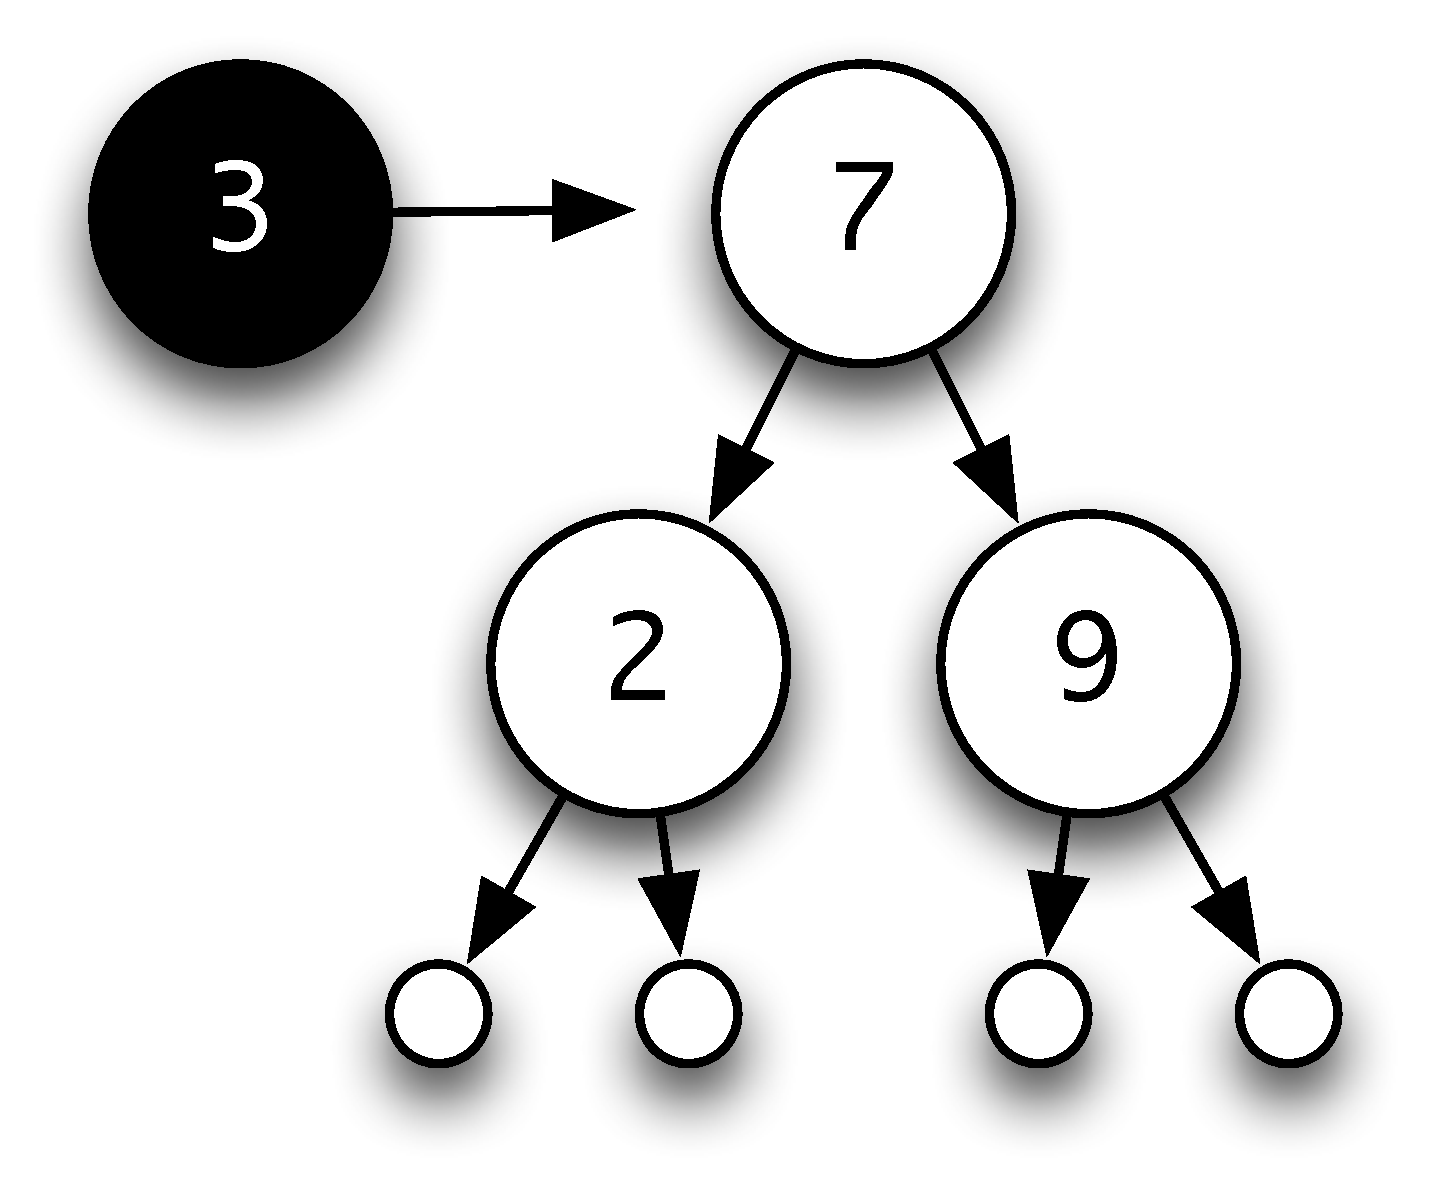
\includegraphics[width=1.3in]{Pictures/SearchTree1.pdf}\hfill
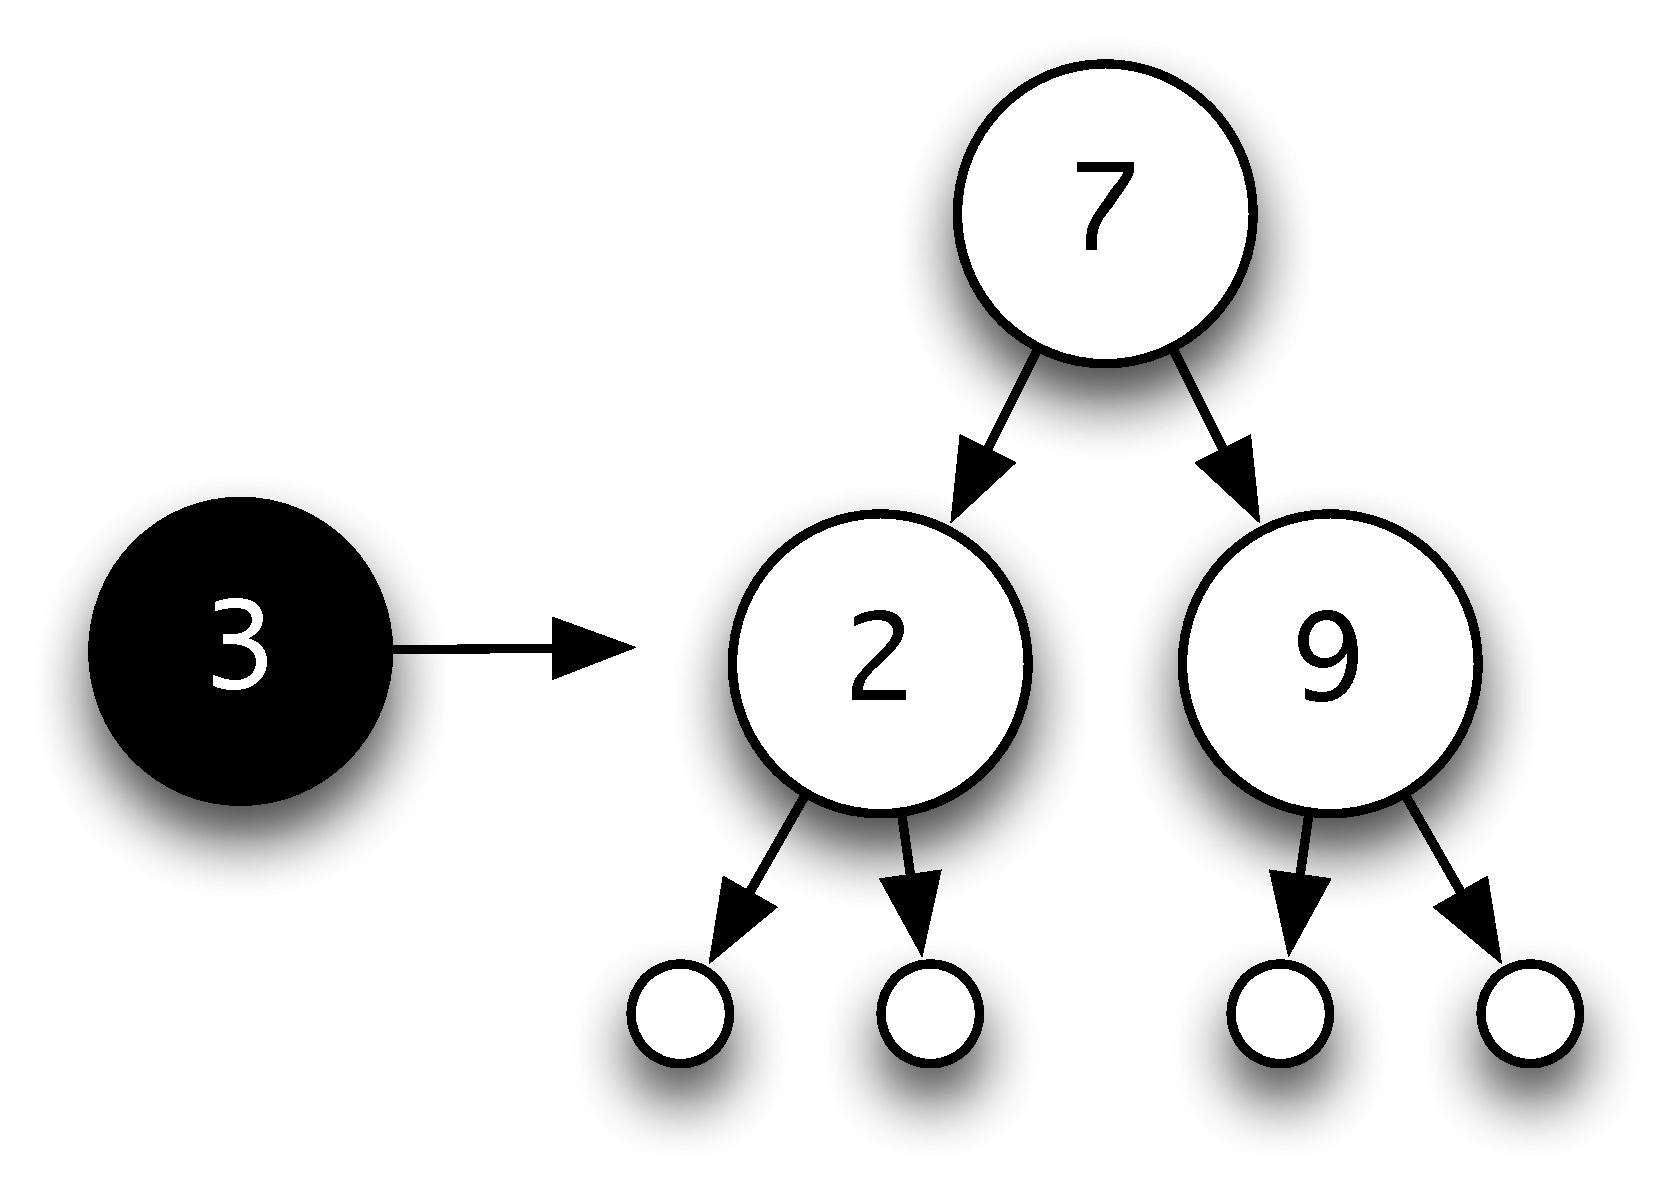
\includegraphics[width=1.5in]{Pictures/SearchTree2.pdf}\hfill
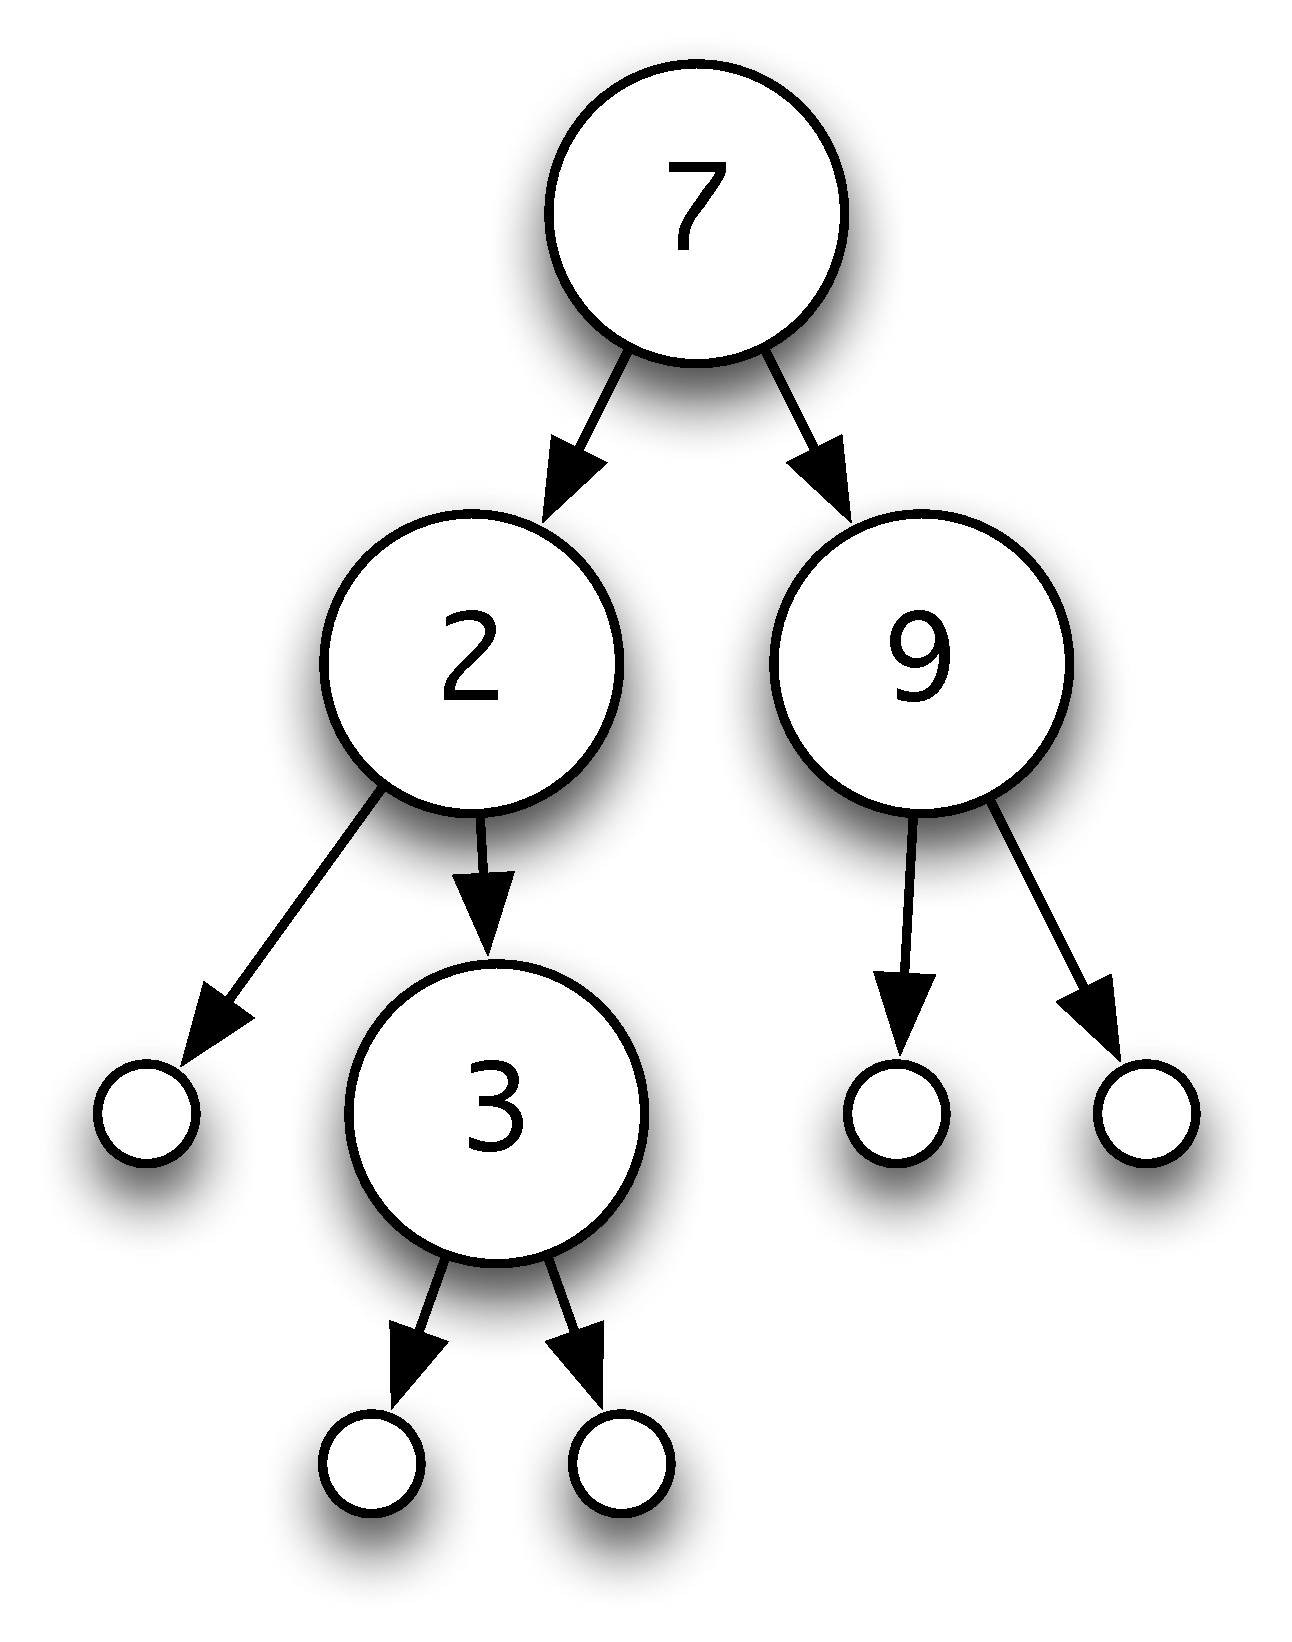
\includegraphics[width=1.2in]{Pictures/SearchTree3.pdf}
\end{center}
\caption{Insertion into a search tree}
\label{insertSearchTree}
\end{figure}



\begin{figure}
\begin{alltt}
insTree :: Ord a => a -> Tree a -> Tree a\minx{insTree}

insTree val Nil = (Node val Nil Nil)

insTree val (Node v t1 t2)
  | v==val      = Node v t1 t2
  | val > v     = Node v t1 (insTree val t2)	
  | val < v     = Node v (insTree val t1) t2	

delete :: Ord a => a -> Tree a -> Tree a\minx{delete}

delete val (Node v t1 t2)
  | val < v     = Node v (delete val t1) t2
  | val > v     = Node v t1 (delete val t2)
  | isNil t2    = t1
  | isNil t1    = t2
  | otherwise   = join t1 t2

minTree :: Ord a => Tree a -> Maybe a\minx{minTree}

minTree t
  | isNil t     = Nothing
  | isNil t1    = Just v
  | otherwise   = minTree t1
      where
      t1 = leftSub t
      v  = treeVal t

--      join is an auxiliary function, used in delete;
--      it is not exported.

join :: Ord a => Tree a -> Tree a -> Tree a\minx{join}

join t1 t2 
  = Node mini t1 newt
    where
    (Just mini) = minTree t2
    newt        = delete mini t2 
\end{alltt}
\caption{Operations over search trees.}
\label{treeOps}
\index{search tree!operations}
\end{figure}
\noindent
Figure \ref{treeOps} contains the definitions of the insertion, deletion and
\index{search tree!insertion}
join functions. The function \texttt{join} is used
to join two trees with the property that all elements in the left are
smaller than all in the right; that will be the case for the call in
\texttt{delete} where it is used. It is not exported, as it can break the ordered property of
search trees if it is applied to an arbitrary pair of search trees.

\begin{figure}[t]
\begin{center}
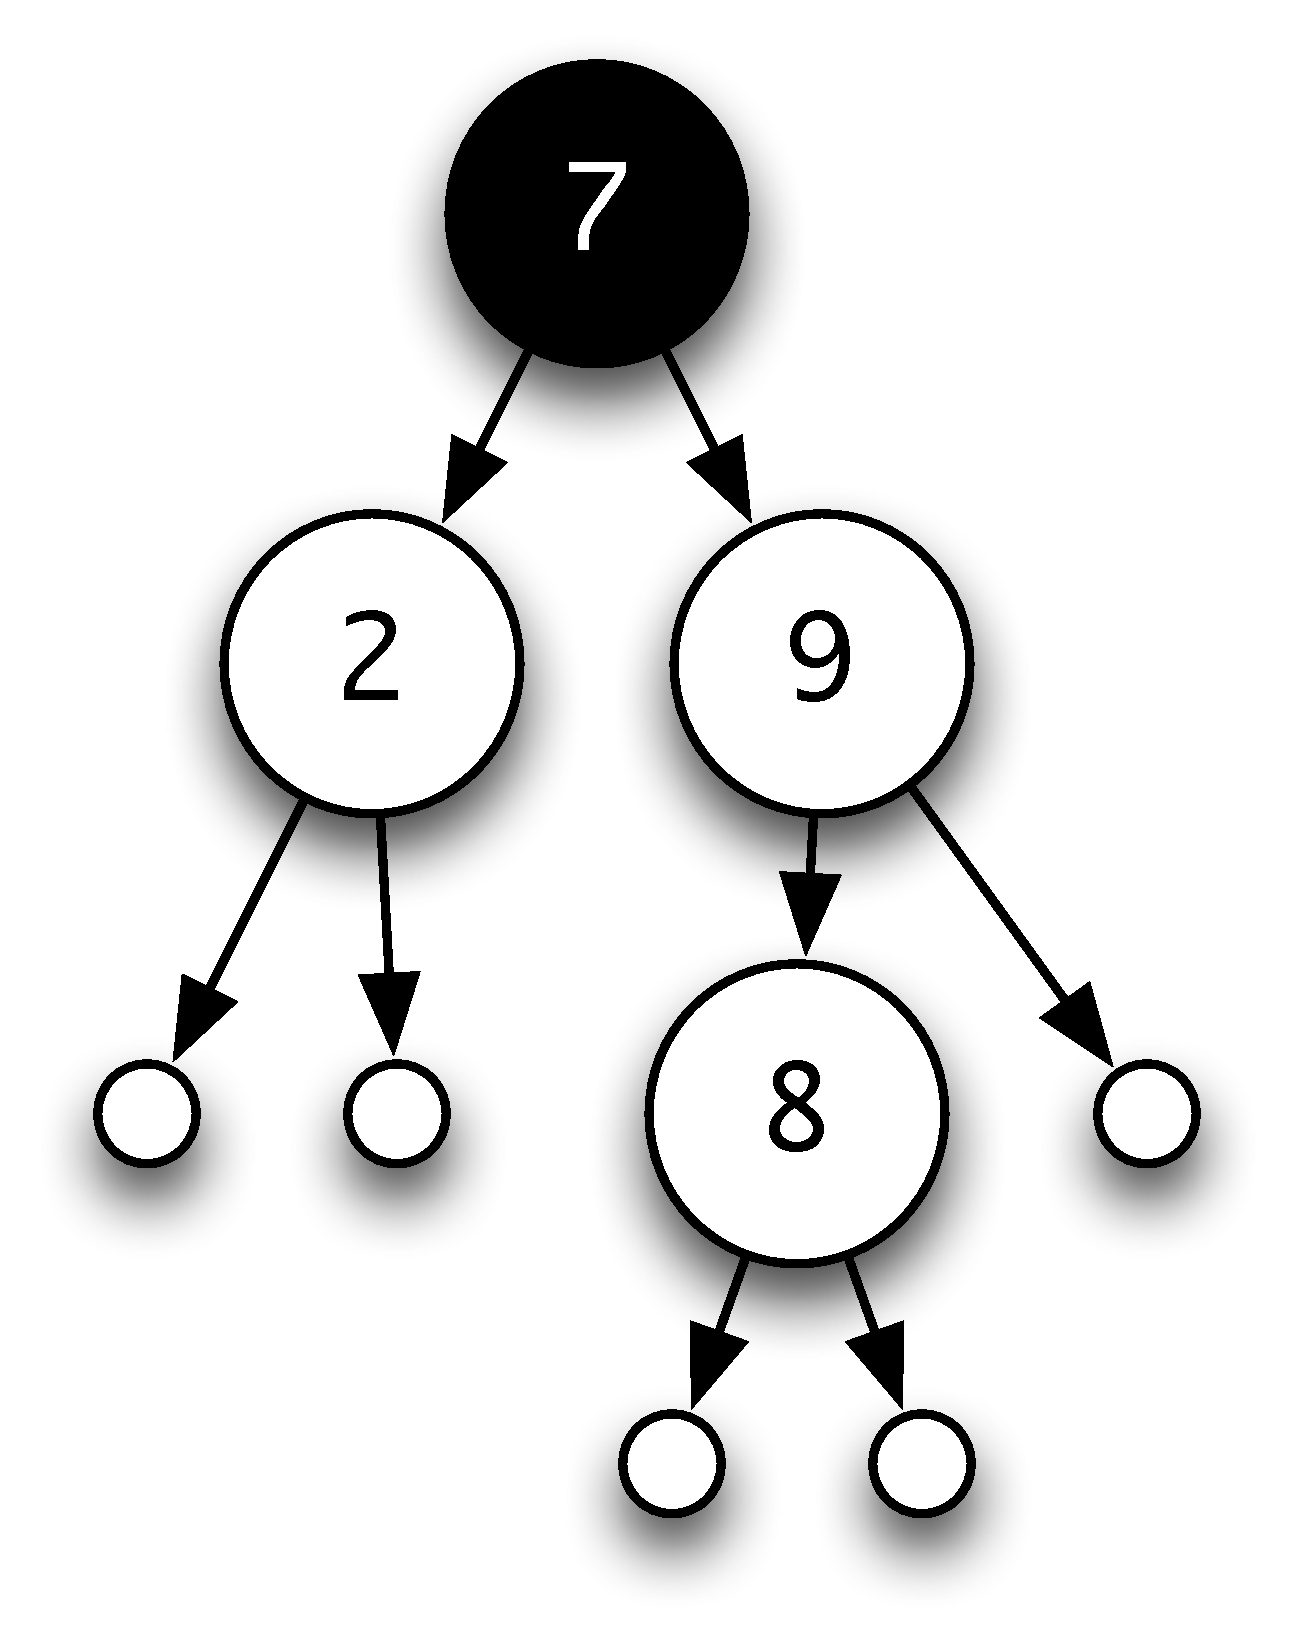
\includegraphics[width=1.1in]{Pictures/SearchTree4.pdf}\hfill
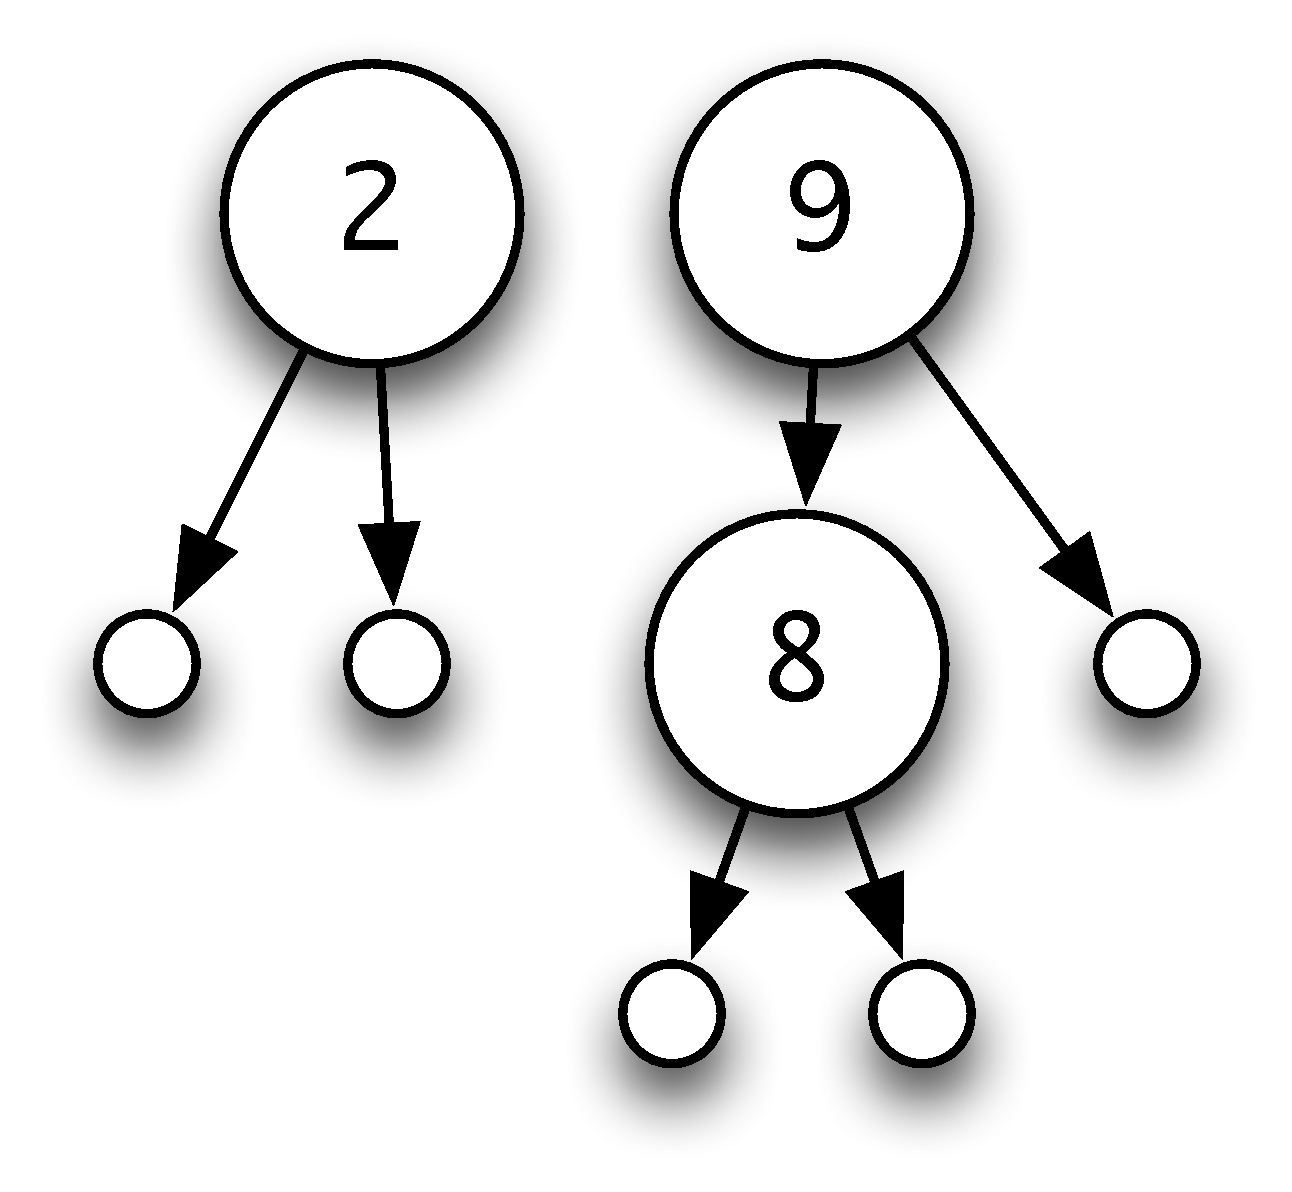
\includegraphics[width=1.1in]{Pictures/SearchTree5.pdf}\hfill
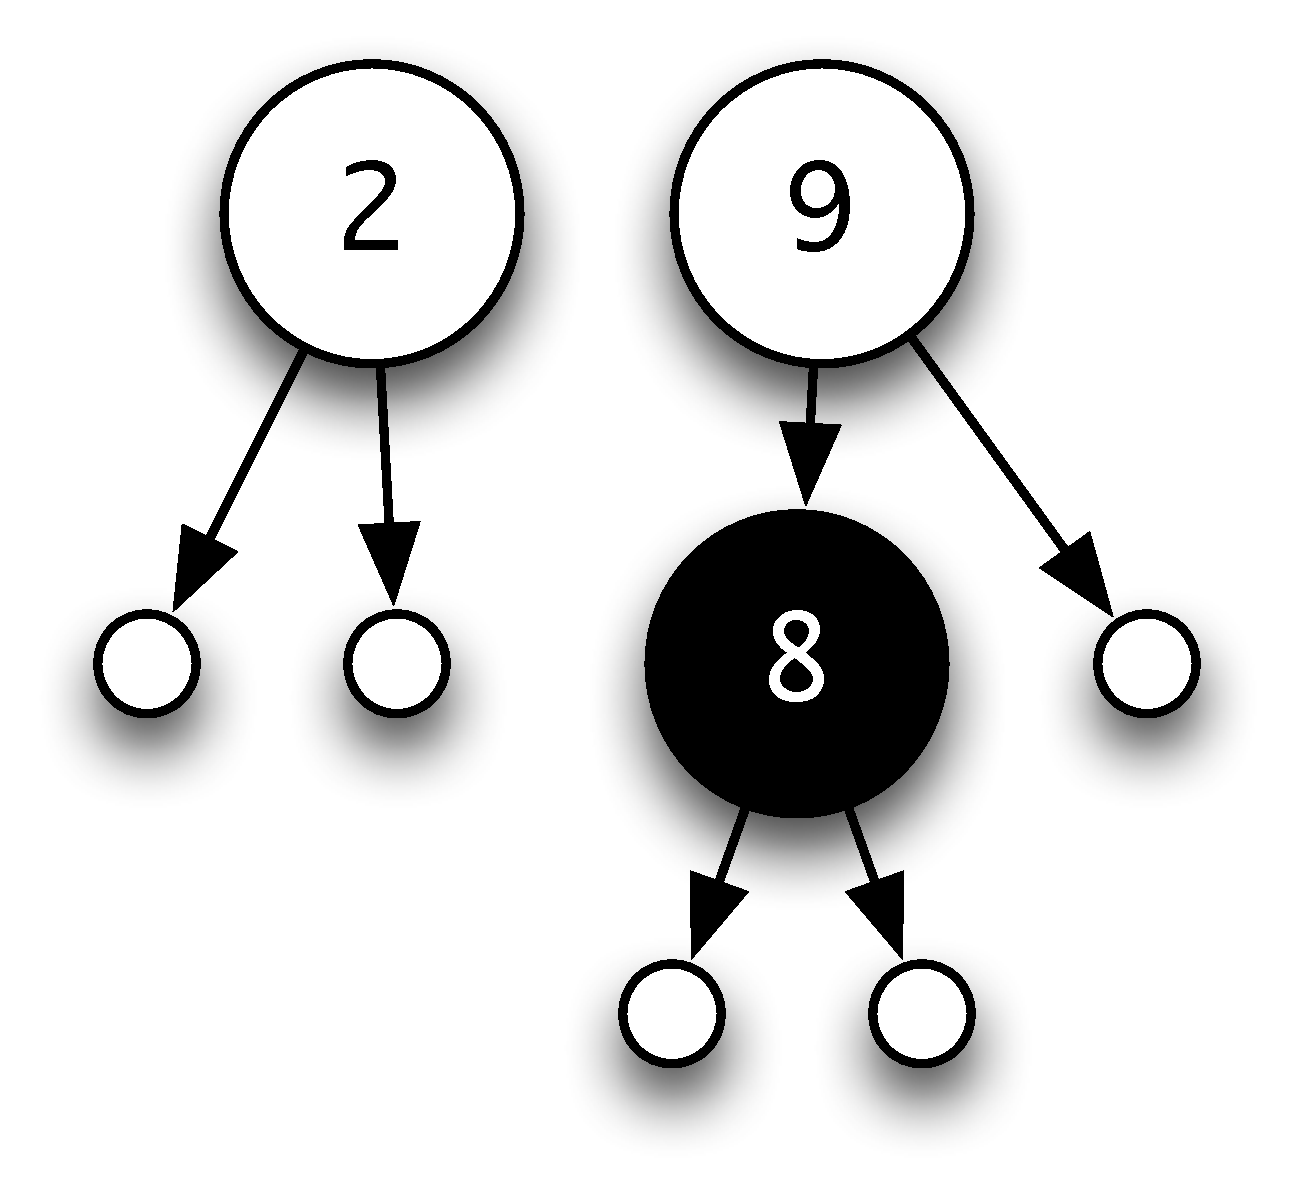
\includegraphics[width=1.1in]{Pictures/SearchTree6.pdf}\hfill
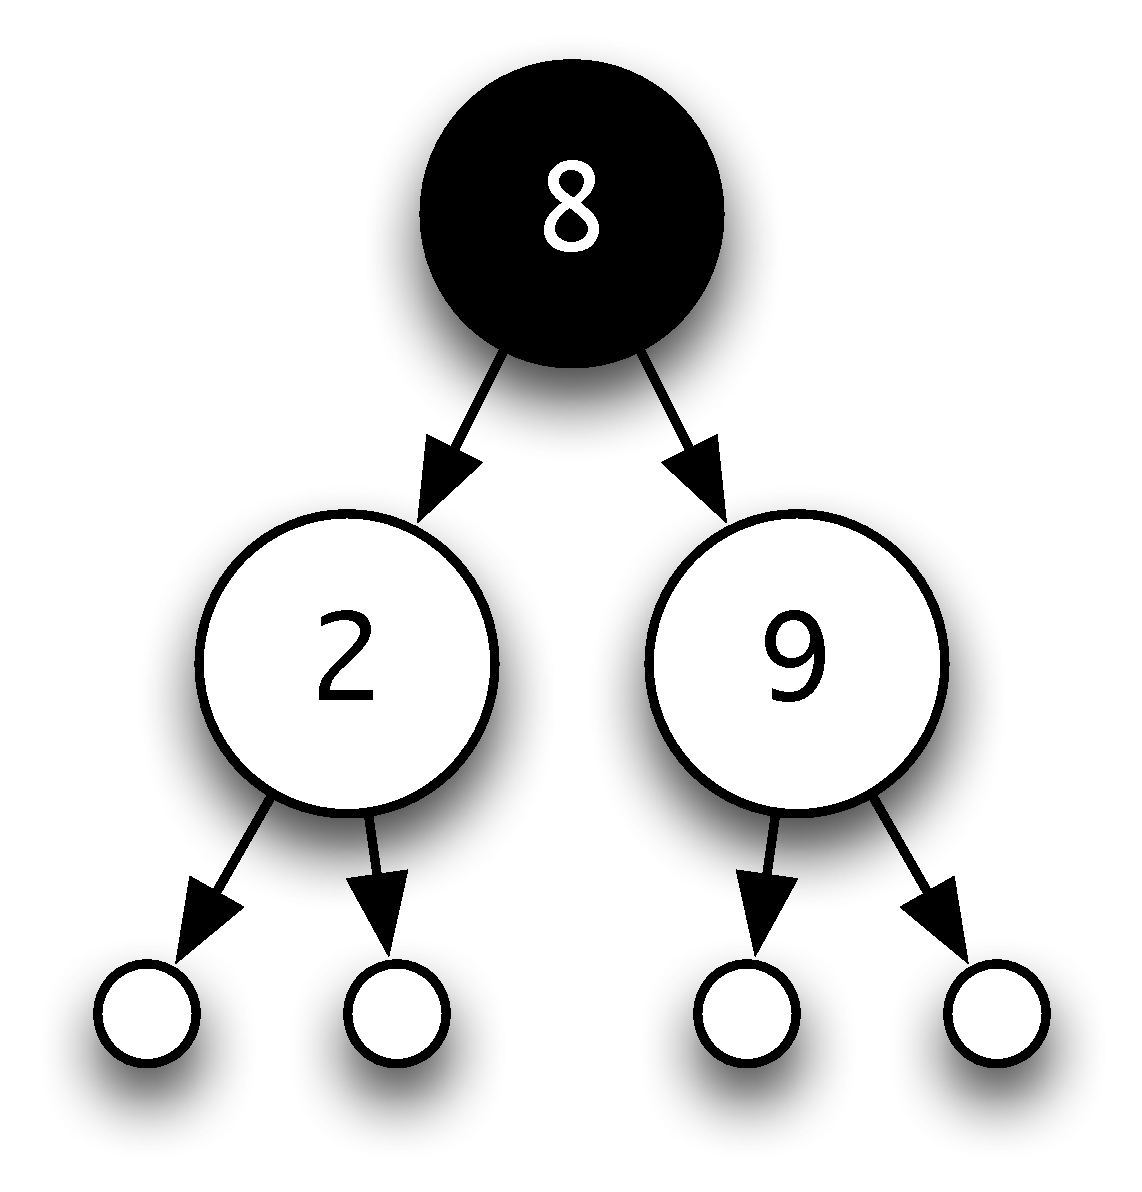
\includegraphics[width=1in]{Pictures/SearchTree7.pdf}
\end{center}
\caption{Deletion from a search tree}
\label{deleteSearchTree}
\end{figure}




Note that the types of \texttt{insTree}, \texttt{delete},
\texttt{minTree} and \texttt{join}
contain the
context \texttt{Ord a}.\minx{Ord}
Recall from Chapter \ref{classes} that this constraint means that
these functions can only be used over types which carry an ordering operation,
\texttt{<=}. It is easy to see from the definitions of these functions that they
do indeed use the ordering, and given the definition of search trees it
is unsurprising that we use an ordering in these operations. Now we look
at the definitions in Figure \ref{treeOps} in turn.

Inserting an element which is already present has no effect,
\index{abstract data type!search tree!insertion}
while inserting an element smaller (larger) than the value at the root causes
it to be inserted in the left (right) subtree. Figure \ref{insertSearchTree} shows \texttt{3} being
inserted in the tree 
\begin{alltt}
(Node 7 (Node 2 Nil Nil) (Node 9 Nil Nil))
\end{alltt}
to give
\begin{alltt}
(Node 7 (Node 2 Nil (Node 3 Nil Nil)) (Node 9 Nil Nil))
\end{alltt}


Deletion is straightforward when the value is smaller (larger) than the value
\index{search tree!deletion}\index{abstract data type!search tree!deletion}
at the root node: the deletion is made in the left (right) sub-tree. If the
value to be deleted lies at the root, deletion is again simple if either
sub-tree is \texttt{Nil}: the other sub-tree is returned. The problem comes when
both sub-trees are non-\texttt{Nil}. In this case, the two sub-trees have to be
joined together, keeping the ordering intact. 

To \texttt{join} two non-\texttt{Nil} trees \texttt{t1} and \texttt{t2}, where it is assumed that
\texttt{t1} is smaller than \texttt{t2}, we pick the
minimum element, \texttt{mini}, of \texttt{t2} to be the value at the root. The left
sub-tree is \texttt{t1}, and the right is given by deleting \texttt{mini} from 
\texttt{t2}. Figure \ref{deleteSearchTree}  shows the deletion of
\texttt{7} from
\begin{alltt}
(Node 7 (Node 2 Nil Nil) (Node 9 (Node 8 Nil Nil) Nil))
\end{alltt} 
to give
\begin{alltt}
(Node 8 (Node 2 Nil Nil) (Node 9 Nil Nil))
\end{alltt} 
The \texttt{minTree} function returns a value of type
\texttt{Maybe a}, since a \texttt{Nil} tree has no minimum. The \texttt{Just} constructor
therefore has to be removed in the \texttt{where} clause of \texttt{join}.

\subsection*{Modifying the implementation}
\index{abstract data type!modifying implementation}
\index{program modification}

Given a search tree, we might be asked for its \texttt{n}th element, 
\begin{alltt}
indexT :: Int -> Tree a -> a

indexT n t \hfill (indexT)
  | isNil t     = error "indexT"
  | n < st1     = indexT n t1  
  | n == st1    = v           
  | otherwise   = indexT (n-st1-1) t2 
    where
    v   = treeVal t
    t1  = leftSub t
    t2  = rightSub t
    st1 = size t1
\end{alltt}
where the \texttt{size} is given by
\begin{alltt}\minx{size}
size :: Tree a -> Int
size t 
  | isNil t     = 0
  | otherwise   = 1 + size (leftSub t) + size (rightSub t)
\end{alltt}
If we are often asked to index elements of a tree, we will repeatedly have to
find the \texttt{size} of search trees, and this will require computation.

We can think of making the size operation more efficient by {\em changing the 
implementation\/} of \texttt{Tree a}, so that an extra field is given in an
\texttt{Stree} to hold the size of the tree:
\begin{alltt}\minx{Stree}
data Stree a = Nil | Node a Int (Stree a) (Stree a)
\end{alltt}
What will have to be changed? 
\begin{titemize}
\item 
We will have to redefine all the operations in the signature, since
they access the implementation type, and this has changed. For example, the
insertion function has the new definition
\begin{alltt} 
insTree val Nil = (Node val 1 Nil Nil)

insTree val (Node v n t1 t2)
  | v==val      = Node v n t1 t2
  | val > v     = Node v (1 + size t1 + size nt2) t1 nt2
  | val < v     = Node v (1 + size nt1 + size t2) nt1 t2
    where
    nt1 = insTree val t1
    nt2 = insTree val t2
\end{alltt}
\item 
We will have to add \texttt{size} to the
signature, and redefine it thus:
\begin{alltt}
size Nil            = 0
size (Node _ n _ _) = n
\end{alltt}
to use the value held in the tree.
\end{titemize}
Nothing else needs to be changed, however. In particular, the definition of
\texttt{indexT} given in \texttt{(indexT)} is unchanged. This is a powerful argument
in favour of using abstract data type
definitions, and against using
pattern matching. If \texttt{(indexT)} had used a pattern match over its argument,
then it would have to be rewritten if the underlying type changed. This
shows that ADTs make programs more easily modifiable, as we argued
at the start of the chapter.

In conclusion, it should be said that these search trees form a model for
a collection of types, as they can be modified to
carry different sorts of information. For, example, we could carry a count of
the number of times an element occurs. This would be increased when an element
is inserted, and reduced by one on deletion. Indeed any type of
additional information can be held at the nodes -- the insertion, deletion
and other operations use the ordering on the elements to structure the tree
irrespective of whatever else is held there. An example might be to store
indexing information together with a word, for instance. This would form the
basis for a reimplementation of the indexing system of Section
\index{document index}
\ref{indexExam}.
\index{search tree|)}

\begin{exercises}

\item
Explain how you would {\em test\/} the implementations of the functions over
search trees. You might need to augment the signature of the type with a
function to print a tree.


\item
Define QuickCheck properties which will test the implementation of search trees. We will show how to define the appropriate generators needed to perform the tests in Chapter \ref{dsls}.




\item
 Define the functions
\begin{alltt}
successor :: Ord a => a -> Tree a -> Maybe a
closest   :: Int -> Tree Int -> Int 
\end{alltt}
The successor of \texttt{v} in a tree \texttt{t} is the smallest value in \texttt{t} larger
than \texttt{v}, while the closest value to \texttt{v} in a numerical tree \texttt{t}
is a value in \texttt{t} which has the smallest difference from \texttt{v}. 
You
can assume that \texttt{closest} is always called on a non-\texttt{Nil} tree, so
always returns an answer.

\item
Redefine the functions of the \texttt{Tree a} signature over the
\texttt{Stree} implementation type.

\item
To speed up the calculation of \texttt{maxTree} and other functions, you could
imagine storing the maximum and minimum of the sub-tree at each node.
Redefine the functions of the signature to manipulate these maxima and
minima, and redefine the functions \texttt{maxTree}, \texttt{minTree} and 
\texttt{successor} to make use of this extra information stored in the trees. 

\item
You are asked to implement search trees with a count of the number of times an
element occurs. How would this affect the signature of the type? How would
you implement the operations? How much of the previously written
implementation could be re-used?

\item
Using a modified version of search trees instead of lists, reimplement the
indexing software of Section \ref{indexExam}.

\item
Design a polymorphic abstract data type
\begin{alltt}
Tree a b c
\end{alltt}
so that entries at each node contain an item of type \texttt{a}, on which the
tree is ordered, and an item of type \texttt{b}, which might be something like
the count, or a list of index entries. 

\hskip1em On inserting an element, information
of type \texttt{c} is given (a single index entry in that example); this
information has to be combined with the information already present. The
method of combination can be a functional parameter. There also needs to be a
function to describe the way in which information is transformed at deletion.

\hskip1em As a test of your type, you should be able to implement the count trees and
the index trees as instances.

\end{exercises}


\section{Sets}
\label{caseSets}
\index{case studies!sets|see{sets}}
\index{sets|(}


A finite set is a collection of
elements of a particular type, which is both like and unlike a list. Lists
are, of course, familiar, and examples include
\begin{alltt}
[Joe,Sue,Ben]     [Ben,Sue,Joe]
[Joe,Sue,Sue,Ben] [Joe,Sue,Ben,Sue]
\end{alltt}
Each of these lists is different -- not only do the elements of a list matter,
but also the \textbf{order} in which they occur and the number of times that
each element occurs (its \textbf{multiplicity}) are significant.\index{multiplicity}
\index{lists!and sets}
\index{sets!and lists}

In many situations, order and multiplicity are irrelevant. If we want to talk
about the collection of people going to a birthday party, we just want the
names; a person is either there or not and so multiplicity is not
important and the order in which we might list them is also of no interest. In other
words, all we want to know is the \textbf{set} of people coming. In the example
above, this is the set consisting of \texttt{Joe}, \texttt{Sue} and \texttt{Ben}.

Like lists, queues, trees and so on,
sets can be combined in many different ways:
the operations which combine sets form the signature of the abstract data type.
The search trees we saw
earlier provide operations which concentrate on elements of a single ordered
set:
`what is the successor of element \texttt{e} in set \texttt{s}?' for instance. 

In
this section we focus on the combining operations for sets.
The signature
\index{signature}for sets is as follows. We explain the purpose of
the operations at the same time as giving their implementation.
\begin{alltt}\minx{Set}
module Set 
 ( Set ,
  empty              , -- Set a
  sing               , -- a -> Set a
  memSet             , -- Ord a => Set a -> a -> Bool
  union,inter,diff   , -- Ord a => Set a -> Set a -> Set a
  eqSet              , -- Eq a  => Set a -> Set a -> Bool
  subSet             , -- Ord a => Set a -> Set a -> Bool
  makeSet            , -- Ord a => [a] -> Set a
  mapSet             , -- Ord b => (a -> b) -> Set a -> Set b
  filterSet          , -- (a->Bool) -> Set a -> Set a
  foldSet            , -- (a -> a -> a) -> a -> Set a -> a
  showSet            , -- (a -> String) -> Set a -> String
  card                 -- Set a -> Int
 ) where
\end{alltt}
There are numerous possible signatures for sets, some of which assume certain
properties of the element type. To test for elementhood, we need the elements
to belong to a type in the \texttt{Eq} class; here we assume that the elements
are in fact from an ordered type, which enlarges the class of operations over
\texttt{Set a}. This gives the contexts 
\texttt{Ord a} and \texttt{Ord b}, which are seen in some of the types in the signature
above.

\subsection*{Implementing the type and operations}

We choose to represent a set as an \textbf{ordered list of
elements without repetitions}:
\begin{alltt}
newtype Set a = Set [a]
\end{alltt}
The principal definitions over \texttt{Set a} are given in Figures
\ref{setDefs1} and \ref{setDefs2}. At the start of the file we see that 
we import the library \texttt{List}, but as there is
a definition of \texttt{union} in there we have to hide this
on import, thus,
\begin{alltt}
import List hiding ( union )
\end{alltt}
Also at the start of the file we give the \texttt{instance} declarations
for the type. It is important to list these at the start because there
is no explicit record of them in the \texttt{module} header.
\index{modules!instance declarations}

We now run through the individual functions as they are implemented in Figures
\ref{setDefs1} and \ref{setDefs2}. In our descriptions we use
curly brackets `\texttt{\{}', `\texttt{\}}', to
represent sets in examples -- this is emphatically not part of Haskell notation.

\paragraph{Empty set and singleton.}
The empty set \texttt{\{\}} is represented by an empty list, and the singleton 
set \texttt{\{x\}},
consisting of the single element \texttt{x}, by a one-element list.
\begin{figure}
\begin{alltt}
import List hiding ( union )

instance Eq a => Eq (Set a) where
  (==) = eqSet
instance Ord a => Ord (Set a) where
  (<=) = leqSet

newtype Set a = Set [a]\minx{Set}

empty :: Set a\minx{empty}
empty  = Set []

sing :: a -> Set a\minx{sing}
sing x = Set [x]

memSet :: Ord a => Set a -> a -> Bool\minx{memSet}
memSet (Set []) y     = False
memSet (Set (x:xs)) y 
  | x<y         = memSet (Set xs) y\hfill(memSet.1)
  | x==y        = True\hfill(memSet.2)
  | otherwise   = False\hfill(memSet.3)

union :: Ord a => Set a -> Set a -> Set a\minx{union}
union (Set xs) (Set ys) = Set (uni xs ys)

uni :: Ord a => [a] -> [a] -> [a]
uni [] ys       = ys
uni xs []       = xs
uni (x:xs) (y:ys) 
  | x<y         = x : uni xs (y:ys)
  | x==y        = x : uni xs ys
  | otherwise   = y : uni (x:xs) ys

inter :: Ord a => Set a -> Set a -> Set a\minx{inter}
inter (Set xs) (Set ys) = Set (int xs ys)

int :: Ord a => [a] -> [a] -> [a]
int [] ys       = []
int xs []       = []
int (x:xs) (y:ys) 
  | x<y         = int xs (y:ys)
  | x==y        = x : int xs ys
  | otherwise   = int (x:xs) ys
\end{alltt}
\caption{Operations over the set abstract data type, part 1.}
\label{setDefs1}
\index{sets!operations}
\end{figure}

\begin{figure}
\begin{alltt}
subSet :: Ord a => Set a -> Set a -> Bool\minx{subSet}
subSet (Set xs) (Set ys) = subS xs ys

subS :: Ord a => [a] -> [a] -> Bool
subS [] ys      = True
subS xs []      = False
subS (x:xs) (y:ys) 
  | x<y         = False
  | x==y        = subS xs ys
  | x>y         = subS (x:xs) ys

eqSet :: Eq a => Set a -> Set a -> Bool\minx{eqSet}
eqSet (Set xs) (Set ys) = (xs == ys)

leqSet :: Ord a => Set a -> Set a -> Bool
leqSet (Set xs) (Set ys) = (xs <= ys)
	
makeSet :: Ord a => [a] -> Set a\minx{makeSet}
makeSet = Set . remDups . sort
          where
          remDups []     = []
          remDups [x]    = [x]
          remDups (x:y:xs) 
            | x < y      = x : remDups (y:xs)
            | otherwise  = remDups (y:xs)

mapSet :: Ord b => (a -> b) -> Set a -> Set b\minx{mapSet}
mapSet f (Set xs) = makeSet (map f xs)

filterSet :: (a -> Bool) -> Set a -> Set a\minx{filterSet}
filterSet p (Set xs) = Set (filter p xs)

foldSet :: (a -> a -> a) -> a -> Set a -> a\minx{foldSet}
foldSet f x (Set xs) = (foldr f x xs)

showSet :: (a->String) -> Set a -> String\minx{showSet}
showSet f (Set xs) = concat (map ((++"\bs{n}") . f) xs)

card :: Set a -> Int\minx{card}
card (Set xs) = length xs
\end{alltt}
\caption{Operations over the set abstract data type, part 2.}
\label{setDefs2}
\index{sets!operations}
\end{figure}

\paragraph{Membership.}
To test for membership of a set, we define \texttt{memSet}. It is important to
see that we exploit the ordering in giving this definition.
Consider the three cases where the list is non-empty. In \texttt{(memSet.1)}, the head
element of the set, \texttt{x}, is smaller than the element \texttt{y} which we seek, and so we
should check recursively for the presence of \texttt{y} in the tail \texttt{xs}. 
In case \texttt{(memSet.2)} we have found
the element, while in case \texttt{(memSet.3)} the head element is larger than
\texttt{y}; since the list is ordered, all elements will be larger than
\texttt{y}, so it cannot be a member of the list. This definition would 
not work if we chose to use arbitrary lists to represent sets.

\paragraph{Union, intersection, difference.}
The functions \texttt{union,inter,diff} give the union, intersection and difference of two
sets. The union consists of the elements occurring in either set (or both), the
intersection of those elements in both sets and the difference of those
elements in the first but not the second set -- we leave the definition of \texttt{diff}
as an exercise for the reader. For example,
\begin{alltt}
union \{Joe,Sue\}\ \{Sue,Ben\}\ =  \{Joe,Sue,Ben\}
inter \{Joe,Sue\}\ \{Sue,Ben\}\ =  \{Sue\}
diff  \{Joe,Sue\}\ \{Sue,Ben\}\ =  \{Joe\}
\end{alltt}
In making these definitions we again exploit the fact that the two arguments
are ordered. We also define the functions by `wrapping up' a function
over the `bare' list type. For instance, in defining \texttt{union} we first
define
\begin{alltt}\minx{union}
uni :: Ord a => [a] -> [a] -> [a]
\end{alltt}
which works directly over ordered lists, and then make a version
which works over \texttt{Set},
\begin{alltt}
union :: Ord a => Set a -> Set a -> Set a
union (Set xs) (Set ys) = Set (uni xs ys)
\end{alltt}
Recall that the brackets  `\texttt{\{}', `\texttt{\}}' are not a part of Haskell; 
we can see them as shorthand for Haskell expressions as follows.
\begin{alltt}
\{\eone, \ldots\ ,\subscr{e}{n}\} = makeSet [\eone, \ldots\ ,\subscr{e}{n}]
\end{alltt}

\paragraph{Subset and equality tests.}
To test whether the first argument is a subset of the second, we use 
\texttt{subSet}; \texttt{x} is a subset of \texttt{y} if every element of \texttt{x} is an
element of \texttt{y}.

Two sets are going to be equal if their representations as ordered lists are
the same -- hence the definition of \texttt{eqSet} as list equality; note that
we require equality on \texttt{a} to define equality on \texttt{Set a}.
The function \texttt{eqSet} is exported as part of the signature, but
also we declare an instance of the \texttt{Eq} class, binding \texttt{==} to \texttt{eqSet}
thus
\begin{alltt}
instance Eq a => Eq (Set a) where\minx{==}
  (==) = eqSet
\end{alltt}
The ADT equality will not in general
be the equality on the underlying type:
if we were to choose arbitrary lists to
model sets, the equality test would be more complex, since \texttt{[1,2]} and
\texttt{[2,1,2,2]} would represent the same set.

\paragraph{Ordering.}
We also export list ordering as an ordering over \texttt{Set}.
\begin{alltt}
instance Ord a => Ord (Set a) where
  (<=) = leqSet
\end{alltt}
The subset ordering is not bound to \texttt{<=} since it is customary
for the \texttt{<=} in \texttt{Ord} to be a total order, that is for all elements
\texttt{x} and \texttt{y}, either \texttt{x<=y} or \texttt{y<=x} will hold. 
\index{order!total}\index{order!partial}
The subset ordering is
not a total order, while the lexicographic ordering over (ordered)
lists is total. Some examples for comparison are given in the exercises.

\paragraph{Construction.}
To form a set from an arbitrary list, \texttt{makeSet}, the list is sorted, and
then duplicate elements are removed, before it is wrapped with \texttt{Set}. 
The definition of \texttt{sort} is
imported from the \texttt{List} library.

\paragraph{Higher-order functions.}
\texttt{mapSet}, \texttt{filterSet} and \texttt{foldSet}
behave like \texttt{map}, \texttt{filter} and \texttt{foldr}
except that they operate over sets. The latter two are essentially given by \texttt{filter}
and \texttt{foldr}; in \texttt{mapSet} duplicates have to be removed after mapping.

\paragraph{Print.}
\texttt{showSet f (Set xs)} gives a printable version of a set, one item per line,
using the function \texttt{f} to give a printable version of each element.
\begin{alltt}
showSet f (Set xs) = concat (map ((++"\bs{n}") . f) xs)
\end{alltt}
\paragraph{Cardinality.}
The cardinality of a set is the number of its members. The function \texttt{card}
gives this, as it returns the \texttt{length} of the list.
 
\medskip\noindent 
In the next section we build a library of functions to work with relations and
graphs which uses the \texttt{Set} library as its basis.

\begin{exercises}

\item
Compare how the following pairs of sets are related by the orderings
\texttt{<=} and \texttt{subSet}.
\begin{alltt}
\{3\}          \{3,4\}
\{2,3\}        \{3,4\}
\{2,9\}        \{2,7,9\}
\end{alltt}

\item
Define the function \texttt{diff} so that \texttt{diff s1 s2} consists of the 
elements of \texttt{s1} which do not belong to \texttt{s2}.  

\item
Define the function
\begin{alltt}
symmDiff :: Ord a => Set a -> Set a -> Set a
\end{alltt}
which gives the \textbf{symmetric difference} of two sets. This consists of the
elements which lie in one of the sets but not the other, so that
\begin{alltt}
symmDiff \{Joe,Sue\}\ \{Sue,Ben\}\ =  \{Joe,Ben\}
\end{alltt}
Can you use the function \texttt{diff} in your definition?

\item
How can you define the
function
\begin{alltt}
powerSet :: Ord a => Set a -> Set (Set a)
\end{alltt}
which returns the set of all
subsets of a set defined? Can you give a definition which uses only the
operations of the abstract data type and not the concrete implementation?

\item
How are the
functions
\begin{alltt}
setUnion :: Ord a => Set (Set a) -> Set a
setInter :: Ord a => Set (Set a) -> Set a
\end{alltt}
which return the union and intersection
of a set of sets defined using the operations of the abstract data type?

\item
Can infinite sets (of numbers, for instance) be adequately
represented by ordered lists? Can you tell if two infinite lists are equal,
for instance?

\item
The abstract data type \texttt{Set a} can be represented in a number of different ways.
Alternatives include  arbitrary lists (rather than ordered lists without
repetitions) and Boolean valued functions, that is elements of the type 
\texttt{a -> Bool}. Give implementations of the type using these two representations.

\item
Give an implementation of the \texttt{Set} abstract data type using search trees.

\item
Give an implementation of the search tree abstract data type using ordered lists. Compare
the behaviour of the two implementations.


\item
Give a set of QuickCheck properties for the \texttt{Set} type. These should reflect the mathematical properties of sets. \emph{Hint:} you could begin by thinking about corresponding properties of lists, and about which of these you would expect to hold for sets and which would not.


\index{sets|)}

\end{exercises}

\section{Relations and graphs}
\label{rels}


We now use the \texttt{Set} abstract data type as a means of implementing relations and,
taking an alternative view of the same objects, graphs.
\vspace{-5pt}

\subsection*{Relations}
\index{relations|(}

A binary relation\index{relation}
relates together certain elements of a set. A family
relationship
can be summarized by saying that
the \texttt{isParent} relation holds between \texttt{Ben} and \texttt{Sue}, between
\texttt{Ben} and \texttt{Leo} and between \texttt{Sue} and \texttt{Joe}. In other
words, it relates the \textbf{pairs} \texttt{(Ben,Sue)}, \texttt{(Ben,Leo)} and 
\texttt{(Sue,Joe)}, and so we can think of this particular relation as the set
\begin{alltt}
isParent = \{(Ben,Sue) , (Ben,Leo) , (Sue,Joe)\}
\end{alltt}
In general we say
\begin{alltt}
type Relation a = Set (a,a)\minx{Relation}
\end{alltt}
This definition means that all the set operations are available on relations.
We can test whether a relation holds of two elements using \texttt{memSet}; the
\texttt{union} of two relations like \texttt{isParent} and \texttt{isSibling} gives
the relationship of being either a parent {\em or\/} a sibling, and so on.

We look at two examples of \textbf{family relations},
\index{relation!family relations} based on a relation \texttt{isParent}\minx{isParent}
which we assume is given to us. We first set ourselves the task of defining the function
\texttt{addChildren} which adds to a set of people all their children; we then aim to define
the \texttt{isAncestor} relation. The full code for the functions discussed here is given in
Figure
\ref{relFuns}.
\begin{figure}
\begin{alltt}
image :: Ord a => Relation a -> a -> Set a\minx{image}
image rel val = mapSet snd (filterSet ((==val).fst) rel)
 
setImage :: Ord a => Relation a -> Set a -> Set a\minx{setImage}
setImage rel = unionSet . mapSet (image rel) 
 
unionSet :: Ord a => Set (Set a) -> Set a\minx{unionSet}
unionSet = foldSet union empty

addImage :: Ord a => Relation a -> Set a -> Set a\minx{addImage}
addImage rel st = st `union` setImage rel st

addChildren :: Set People -> Set People\minx{addChildren}
addChildren = addImage isParent 

\hspace*{0cm}\hrulefill\hspace*{0cm}\\

compose :: Ord a => Relation a -> Relation a -> Relation a\minx{compose}
compose rel1 rel2
  =  mapSet outer (filterSet equals (setProduct rel1 rel2))
     where
     equals ((a,b),(c,d)) = (b==c)
     outer  ((a,b),(c,d)) = (a,d)
 
setProduct :: (Ord a,Ord b) => Set a -> Set b -> Set (a,b)\minx{setProduct}
setProduct st1 st2 = unionSet (mapSet (adjoin st1) st2)
 
adjoin :: (Ord a,Ord b) => Set a -> b -> Set (a,b)\minx{adjoin}
adjoin st el = mapSet (addEl el) st
               where
               addEl el el' = (el',el)
 
tClosure :: Ord a => Relation a -> Relation a\minx{tClosure}
tClosure rel = limit addGen rel
               where
               addGen rel' = rel' `union` (rel' `compose` rel)

limit:: Eq a => (a -> a) -> a -> a\minx{limit}
limit f x 
  | x == next     = x
  | otherwise     = limit f next
    where
    next = f x
\end{alltt}
\caption{Functions over the type of relations, \texttt{Relation a}.}
\label{relFuns}
\index{relation!operations}
\end{figure}

\subsection*{Defining \texttt{addChildren}}

\paragraph{The image of an element.}
Working bottom-up, we first ask how we find all elements related to a given
element: who are all \texttt{Ben}'s children, for instance? We need to find all
pairs beginning with \texttt{Ben}, and then return their second halves. The
function to perform this is called \texttt{image}
and the set of \texttt{Ben}'s children will be 
\begin{alltt}
image isParent Ben = \{Sue,Leo\}
\end{alltt}

\paragraph{The image of a set of elements.}
Now, how can we find all the elements related to a {\em set} of elements? We
find the \texttt{image} of each element separately  and then take the union of
these sets.
The union of a set of sets is given by folding the binary union
operation into the set.
\begin{alltt}
unionSet \{\subscr{s}{1}, \ldots\ ,\subscr{s}{n}\}
  = \subscr{s}{1} \(\cup\) \ldots\ \(\cup\)\ \subscr{s}{n} 
  = \subscr{s}{1} `union` \ldots\ `union` \subscr{s}{n}
\end{alltt}
Now, how do we add all the children to a set of people? We find the image of
the set under \texttt{isParent}, and combine it with the set itself. This is
given by the function \texttt{addChildren}.

\subsection*{Defining \texttt{isAncestor}}

The second task we set ourselves was to find the \texttt{isAncestor}
relation.
The general problem is to find the transitive closure of a
relation, the function \texttt{tClosure}\minx{tClosure} of Figure \ref{relFuns}. We do this by
closing up the relation, so we add grandparenthood,  great-grandparenthood
and so forth to the relation until nothing further is added. We explain
transitive closure formally later in this section.

\paragraph{The `grandparent' relation: relational composition.}
How do
we define the relation \texttt{isGrandparent}? We match together pairs like
\begin{alltt}
(Ben,Sue)    (Sue,Joe)
\end{alltt}
and see that this gives that \texttt{Ben} is a grandparent of \texttt{Joe}. We call
this the relational composition\index{relation!composition}
of \texttt{isParent} with itself. In general,
\begin{alltt}
isGrandparent 
  = isParent `compose` isParent
  = \{(Ben,Joe)\}
\end{alltt}

\paragraph{Set product.}
In defining \texttt{compose}
we have used the \texttt{setProduct} function to give the product of
\index{sets!product}
two sets. This is formed by pairing every element of the first set with every
element of the second. For instance,
\begin{alltt}
setProduct \{Ben,Suzie\}\ \{Sue,Joe\} 
  = \{ (Ben,Sue) , (Ben,Joe) , (Suzie,Sue) , (Suzie,Joe) \} 
\end{alltt}
\texttt{setProduct} uses the function \texttt{adjoin} to pair each element of a set
with a given element. For instance,
\begin{alltt}
adjoin \{Ben,Sue\}\ Joe = \{ (Ben,Joe) , (Sue,Joe) \} 
\end{alltt}

\paragraph{Transitive closure and limits.}
A relation \texttt{rel} is \textbf{transitive} if for all\index{relation!transitive} 
\texttt{(a,b)} and \texttt{(b,c)} in \texttt{rel}, \texttt{(a,c)} is in \texttt{rel}.
The transitive closure of a relation \texttt{rel} is the\index{relation!transitive
closure}
smallest relation extending \texttt{rel} which is transitive. We compute the
transitive closure of \texttt{rel}, \texttt{tClosure rel}, by repeatedly adding one
more `generation' of \texttt{rel}, using \texttt{compose}, until nothing more is
added.

To do this, we make use of the \texttt{limit}\minx{limit} function,
 a polymorphic higher-order function of
general use. \texttt{limit f x}\minx{limit} gives the \textbf{limit} of the sequence
\begin{alltt}
x , f x , f (f x) , f (f (f x)) , ...
\end{alltt}
The
limit is the value to which the sequence settles down if it exists. It is
found by taking the first element in the sequence whose successor is equal
to the element itself.  
 
\paragraph{Example.}
As an example, take \texttt{Ben} to be 
\texttt{Sue}'s father, \texttt{Sue} to be \texttt{Joe}'s mother, who himself has no children.
Now define 
\begin{alltt}
addChildren :: Set Person -> Set Person
\end{alltt}
to add to a set the children of all members of the set, so that
for instance
\begin{alltt}
addChildren \{Joe,Ben\} = \{Joe,Sue,Ben\}
\end{alltt}
Now we can give an example calculation of a \texttt{limit} of a function over sets.
\begin{alltt}
limit addChildren \{Ben\}
  ??  \{Ben\}==\{Ben,Sue\} \step False
\step limit addChildren \{Ben,Sue\}
  ??  \{Ben,Sue\}==\{Ben,Joe,Sue\} \step False
\step limit addChildren \{Ben,Joe,Sue\}
  ??  \{Ben,Joe,Sue\}==\{Ben,Joe,Sue\} \step True
\step \{Ben,Joe,Sue\}
\end{alltt}


\beware{Context simplification}{
\index{classes!context simplification}\index{context!simplifying}
The functions of Figure \ref{relFuns} give an interesting example of context 
simplification for type
classes. The \texttt{adjoin} function requires that the types \texttt{a}
and \texttt{b} carry an ordering. Haskell contains the instance declaration
\begin{alltt}
instance (Ord a, Ord b) => Ord (a,b) ....\hfill(pair)
\end{alltt}
and so this is sufficient to ensure \texttt{Ord (a,b)},
which is required for the application of \texttt{mapSet} within \texttt{adjoin}. 

\medskip
Similarly, in defining \texttt{compose} we require an ordering on the type 
\texttt{((a,a),(a,a))}; again, knowing \texttt{Ord a} is sufficient to give this,
since \texttt{(pair)} can be used to derive the ordering on \texttt{((a,a),(a,a))}.
}

\index{relations|)}

\subsection*{Graphs}
\index{graph|(}

Another way of seeing a relation is as a directed \textbf{graph}. For example, the
relation
\begin{alltt}
graph1 = \{ (1,2) , (1,3) , (3,2) , (3,4) , (4,2) , (2,4) \}
\end{alltt}
can be pictured like this
\begin{center}
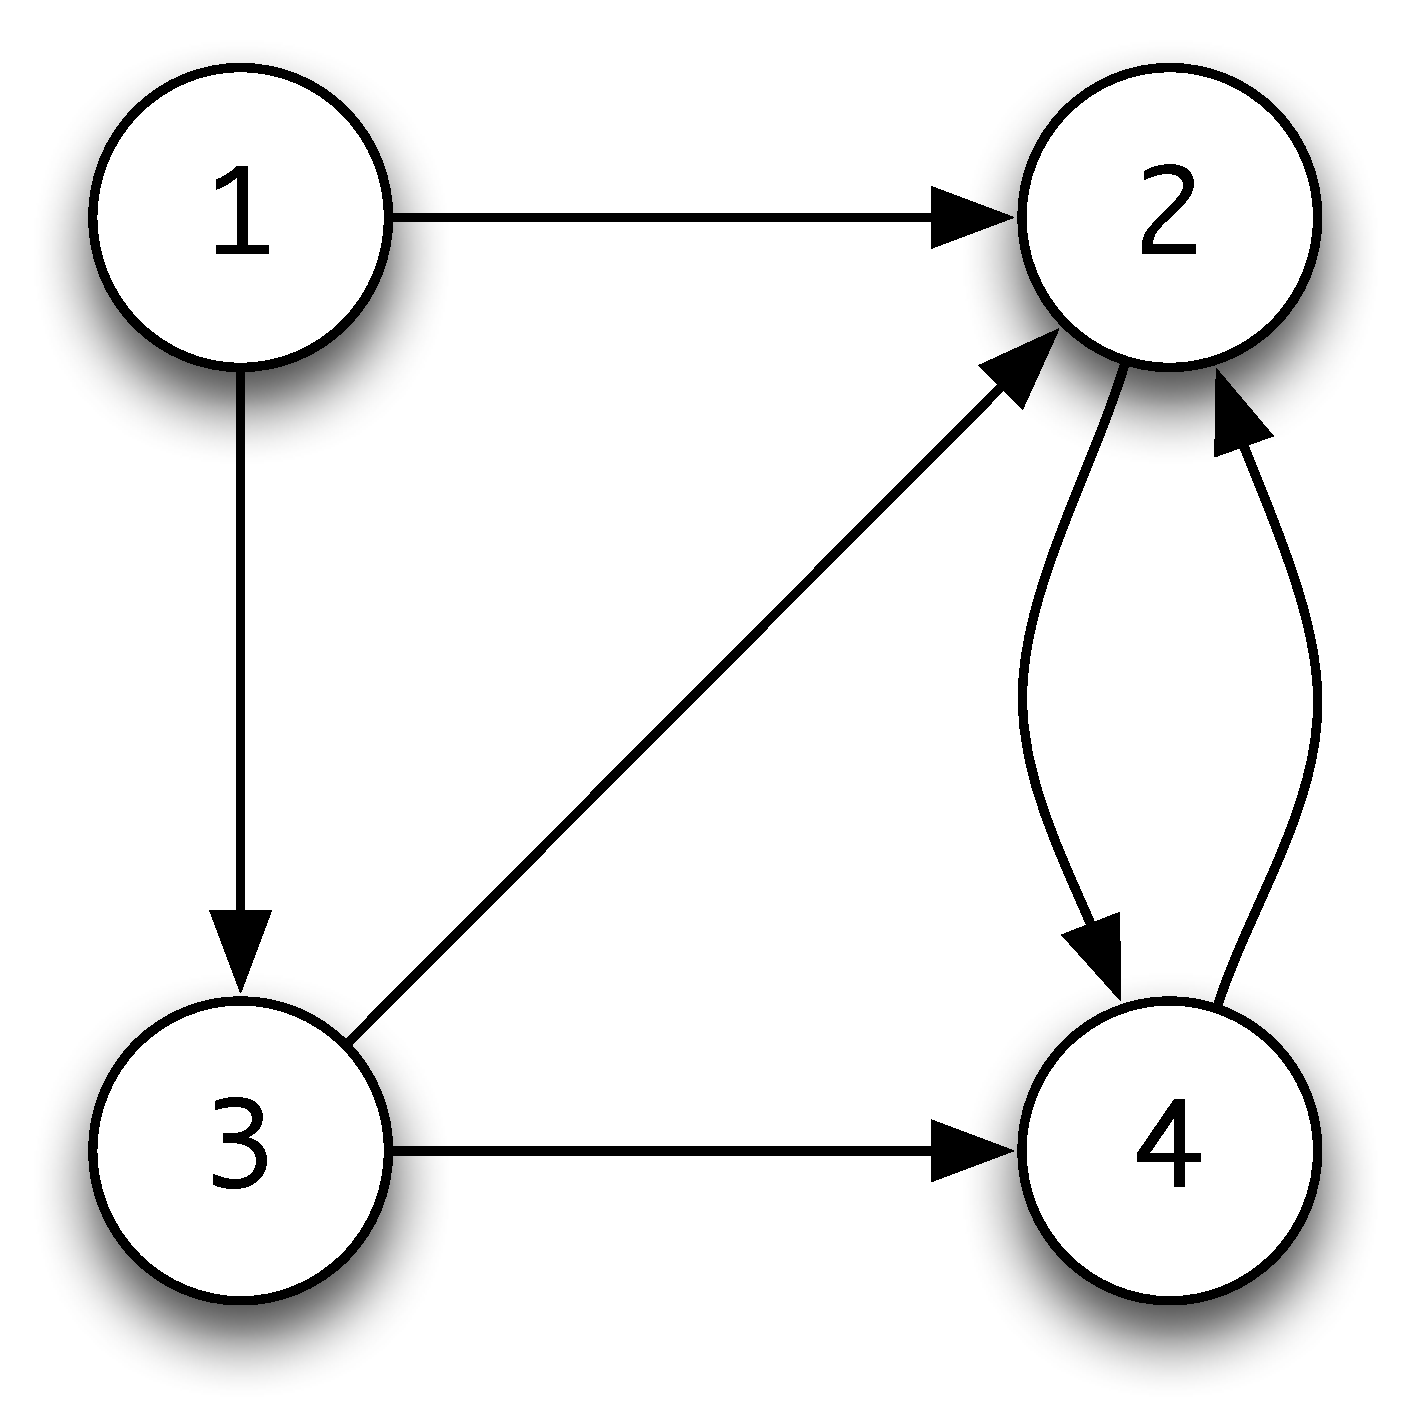
\includegraphics[width=1.5in]{Pictures/Graph.pdf}
\end{center}
where we draw an arrow joining \texttt{a} to \texttt{b} if the pair
\texttt{(a,b)} is in the relation. What then does the transitive closure represent? Two
points
\texttt{a} and \texttt{b} are related by \texttt{tClosure graph1}\minx{tClosure} if there is a
\textbf{path}\index{graph!path in} 
from \texttt{a} to \texttt{b} through the graph. For example, the pair
\texttt{(1,4)} is in the closure, since a path leads from \texttt{1} to \texttt{3}
then to \texttt{2} and finally to \texttt{4}, while the pair \texttt{(2,1)} is not in
the closure, since no path leads from \texttt{2} to \texttt{1} through the graph.

\subsection*{Strongly connected components}

A problem occurring in many different application areas, including networks
and compilers, is to find the \textbf{strongly connected components} of a graph.
\index{graph!strongly connected components}
Every graph can have its nodes split into sets or components with the
property that every node in a component is connected by a path to all
other nodes in the same component. The components of \texttt{graph1} are 
\texttt{\{1\}}, \texttt{\{3\}} and \texttt{\{2,4\}}. 

We solve the problem in two stages:
\begin{titemize}
\item we first form the relation which links points in the same component,
then
\item we form the components (or equivalence classes) generated by this
relation.
\end{titemize}
There is a path from \texttt{x} to \texttt{y} and vice versa if both \texttt{(x,y)}
and \texttt{(y,x)} are in the closure, so we define
\begin{alltt}
connect :: Ord a => Relation a -> Relation a\minx{connect}
connect rel = clos `inter` solc
              where
              clos = tClosure rel
              solc = inverse clos

inverse :: Ord a => Relation a -> Relation a\minx{inverse}
inverse = mapSet swap
          where 
          swap (x,y) = (y,x)
\end{alltt}
Now, how do we form the components given by the relation \texttt{graph1}? We start
with the set 
\begin{alltt}
\{\{1\},\{2\},\{3\},\{4\}\}
\end{alltt}
and repeatedly add the images under the relation to each of the classes,
until a fixed point is reached. In general this gives
\begin{alltt}
classes :: Ord a => Relation a -> Set (Set a)\minx{classes}
classes rel 
  = limit (addImages rel) start
    where
    start = mapSet sing (eles rel)
\end{alltt}
where the auxiliary functions used are
\begin{alltt}
eles :: Ord a => Relation a -> Set a
eles rel = mapSet fst rel `union` mapSet snd rel

addImages :: Ord a => Relation a -> Set (Set a) -> Set (Set a)
addImages rel = mapSet (addImage rel)
\end{alltt}

\subsection*{Searching in graphs}
\index{graph!search}

Many algorithms require us to \textbf{search} through the nodes of a graph: 
we might want to find a shortest path from one point to another, or to
count the number of paths between two points. 

Two general patterns of search are depth-first and breadth-first. In a
depth-first search, we explore all elements below a given child before moving
to the next child; a breadth-first search examines all the children before
examining the grandchildren, and so on. In the case of searching below node
\texttt{1} in \texttt{graph1}, the sequence \texttt{[1,2,4,3]} is depth-first (\texttt{4}
is visited before \texttt{3}), while \texttt{[1,2,3,4]} is breadth-first. These
examples show that we can characterize the searches as functions
\begin{alltt}
breadthFirst :: Ord a => Relation a -> a -> [a]
depthFirst   :: Ord a => Relation a -> a -> [a]
\end{alltt}
with  \texttt{breadthFirst graph1 1 = [1,2,3,4]}, for instance. The use of a
list in these functions is crucial -- we are not simply interested in
finding the nodes below a node (\texttt{tClosure} does this), we are interested
in the {\em order\/} in which they occur.

The essential step in both searches is to find all the descendants of a node which
have not been visited so far. We can write
\begin{alltt}
newDescs :: Ord a => Relation a -> Set a -> a -> Set a
newDescs rel st v = image rel v `diff` st
\end{alltt}
which returns the \textbf{set} of descendants of \texttt{v} in \texttt{rel} which
are not in the set \texttt{st}. Here we have a problem; the result of this
function is a set and not a list, but we require the elements in some order.
One solution is to add to the \texttt{Set} abstract data type a function
\begin{alltt}
flatten :: Set a -> [a]\hfill (setList)
flatten (Set xs) = xs
\end{alltt}
which breaks the abstraction barrier in the case of the ordered list
implementation. An alternative is to supply as a parameter a function
\begin{alltt}
minSet :: Set a -> Maybe a
\end{alltt}
which returns the minimum of a non-empty set
and which can be used in flattening a set to a list without breaking the
abstraction barrier. Unconcerned about its particular definition, we assume the existence
of a flatten function of type \texttt{(setList)}. Then we can say
\begin{alltt}
findDescs :: Ord a => Relation a -> [a] -> a -> [a]
findDescs rel xs v = flatten (newDescs rel (makeSet xs) v)
\end{alltt}

\subsubsection*{Breadth-first search}
\index{graph!search!breadth-first}

A breadth-first search involves repeatedly applying \texttt{findDescs} until a
limit is reached. The \texttt{limit} function discussed earlier will
find this, so we define
\begin{alltt}
breadthFirst :: Ord a => Relation a -> a -> [a]\minx{breadthFirst}
breadthFirst rel val
	= limit step start
	  where
	  start = [val]
	  step xs = xs ++ nub (concat (map (findDescs rel xs) xs))
\end{alltt}
A \texttt{step} performs a number of operations:
\begin{titemize}
\item First, all the descendants of
elements in \texttt{xs} which are not already in \texttt{xs} are found. This is given
by mapping \texttt{(findDescs rel xs)} along the list \texttt{xs}.
\item This list of
lists is then concatenated into a single list.  
\item Duplicates can occur
in this list, as a node may be a descendant of more than one node, 
and so any
duplicated elements must be removed. This is the effect of the library
function
\begin{alltt}\minx{nub}
nub :: Eq a => [a] -> [a]
\end{alltt}
which removes all but the first
occurrence of each element in a list.
\end{titemize}

\subsubsection*{Depth-first search}
\index{graph!search!depth-first}

How does depth-first search proceed? We first generalize the problem to
\index{generalization}
\begin{alltt}
depthSearch :: Ord a => Relation a -> a -> [a] -> [a]\minx{depthSearch}
depthFirst rel v = depthSearch rel v []
\end{alltt}
where the third argument is used to carry the list of nodes already
visited, and which are therefore not to appear in the result of the function call.
\begin{alltt}
depthSearch rel v used
        = v : depthList rel (findDescs rel used' v) used'
          where
          used' = v:used
\end{alltt}
Here we call the auxiliary function \texttt{depthList}, which finds all the
descendants of a list of nodes. 
\begin{alltt}
depthList :: Ord a => Relation a -> [a] -> [a] -> [a]

depthList rel [] used = [] 

depthList rel (val:rest) used
  = next ++ depthList rel rest (used++next)
    where
    next = if   elem val used
           then []
           else depthSearch rel val used
\end{alltt}
The definition has two equations, the first giving the trivial case where no
nodes are to be explored. In the second there are two parts to the solution:
\begin{titemize}
\item \texttt{next} gives the part of the graph accessible below \texttt{val}. This
may be \texttt{[]}, if \texttt{val} is a member of the list \texttt{used}, otherwise
\texttt{depthSearch} is called. 
\item \texttt{depthList} is then called on the tail
of the list, but with \texttt{next} appended to the list of nodes already visited.
\end{titemize}
This pair of definitions is a good example of definition by \textbf{mutual
recursion}\index{recursion!mutual}, since each calls the other. It is possible to define a single
function to perform the effect of the two, but this pair of functions seems
to express the algorithm in the most natural way.

\index{graph|)}


\begin{exercises}

\item
Calculate
\begin{alltt}
classes (connect graph1)
classes (connect graph2)
\end{alltt}
where \texttt{graph2 = graph1 \(\cup\) \{(4,3)\}}.

\item
Give calculations of 
\begin{alltt}
breadthFirst graph2 1
depthFirst graph2 1
\end{alltt}
where \texttt{graph2} is defined in the previous question.

\item
Using the searches as a model, give a function
\begin{alltt}
distance :: Eq a => Relation a -> a -> a -> Int
\end{alltt}
which gives the length of a shortest path from one node to another in a
graph. For instance,
\begin{alltt}
distance graph1 1 4 = 2
distance graph1 4 1 = 0
\end{alltt}
\texttt{0} is the result when no such path exists, or when the two nodes are
equal. 

\item
A weighted graph carries a numerical \textbf{weight} with each edge. Design a type to
model this. Give functions for breadth-first and depth-first search which
return lists of pairs. Each pair consists of a node, together with the
length of a shortest path to that node from the node at the start of the
search.

\item
A \textbf{heterogeneous} relation relates objects of different type. An
example might be the relation relating a person to their age. Design a type
to model these relations; how do you have to modify the functions defined over
\texttt{Relation a} to work over this type, if it is possible?


\item {[Harder]}
Formulate QuickCheck properties for the search functions given in this section. You should try to think of properties which are shared by all search functions, and also other properties which hold of particular search functions.





\end{exercises}



\section{Commentary}
\label{adtCommentary}

This section explores a number of issues raised by the introduction of ADTs
into our repertoire.

First, we
have not yet said anything about verification of functions over abstract
data types.
\index{proof!abstract data types and}
This is because there is nothing new to say about the {\em proof\/} of
theorems: these are proved for the implementation types exactly as we have
seen earlier. The theorems valid for an abstract data type
are precisely those which
obey the type constraints on the functions in the signature. For a queue type,
for instance, we will be able to prove that
\begin{alltt}
remQ (addQ x emptyQ) = (x , emptyQ)
\end{alltt}
by proving the appropriate result about the implementation. What would not be
valid would be an equation like 
\begin{alltt}
emptyQ = Qu []
\end{alltt}
since this breaks the information-hiding barrier and reveals something of the
implementation itself.

Next we note that our
implementation of sets gives rise to some properties which we
ought to prove, often called \textbf{invariants}.
\index{invariant}
We have assumed that our sets
are implemented as ordered lists without repetitions; we ought to prove that
each operation over our implementation preserves this property.
Both the properties of the functions, and the invariants over the implementation, can be formulated as QuickCheck properties; we leave these as exercises for the reader.

Finally, observe that both classes and
abstract data types use signatures, so it is worth surveying
their similarities and differences.
\index{classes!and ADTs}\index{signature}
\index{abstract data type!and classes}
\begin{titemize}
\item Their purposes are different: ADTs are used to provide information
hiding, and to structure programs; classes are used to overload names, to
allow the same name to be used over a class of different types.
\index{signature}
\item The signature in an ADT is associated with a single implementation
type, which may
be monomorphic or polymorphic. On the other hand, the signature in a class
will be associated with multiple instances; this is the whole point of
including classes, in fact.
\item The functions in the signature of an ADT provide the only access
to the underlying type. There is no such information hiding over classes: to
be a member of a class, a type must provide at least the types in
signature.
\end{titemize}

\begin{summary}
The abstract data types of this chapter have three
important and related properties.
\begin{titemize}
\item They provide a natural representation of a type,
which avoids being over-specific. An abstract data type carries precisely
the operations which are naturally associated with the type  and
nothing more.
\item The signature of an abstract data type
is a firm interface between the user
and the implementer: development of a system can proceed completely
independently on the two sides of the interface.
\item If the implementation of a type is to be modified,
then only the operations in the signature need to be changed;
any operation using the signature functions can be used
unchanged. We saw an example of this with search trees, when
the implementation  was modified to include size information.
\end{titemize}
We saw various examples of ADT development. Most importantly we saw
the practical example of the simulation types being designed in the three
stages suggested. First the types are named, then they are described
informally  and finally a signature is written down. After that we are able
to implement the operations of the signature as a separate task.

One of the difficulties in writing a signature is being sure that all the
relevant operations have been included; we have given a check-list of the kinds of
operations which should be present, and against which it is sensible to
evaluate any candidate signature definitions. 


\end{summary}


%\end{document}

%\documentclass{book}\usepackage{sjtfonts}\usepackage{includegraphics}\usepackage{alltt}\usepackage{latexsym}
%\usepackage{array}
%\begin{document}\input{defs0}%		miradefs.tex 		    June 1994

% opening and closing a quoted Miranda section

\newcommand{\mira}{\noindent\hrulefill\nopagebreak\so}
\newcommand{\arim}{\nopagebreak\st\hrulefill\\}

% backslash in the Miranda environment
% Only feasible approach is to use \verb+\+
% in line!

%\newcommand{\bs}{$\mi\backslash\!\!$}
%\newcommand{\lbs}{\mbox{\verb+\+}}

% ignoring part of the input

\newcommand{\ignore}[1]{}

% a blank line in a Miranda section

\newcommand{\bl}{\mbox{\ }}

% Signalling a diffculty.

\definecolor{light-gray}{gray}{0.95}

\newcommand{\beware}[2]
 {\medskip\noindent\colorbox{light-gray}{\parbox{\textwidth}
 {\mbox{\large\textbf{#1}} \medskip\noindent\\ #2}\medskip\noindent}}

% Subscripting in Miranda text
\newcommand{\subscr}[2]{\mbox{${\mbox{\texttt{#1}}}_{\mbox{\texttt{#2}}}$}}

%\newcommand{\subscr}[2]{\mbox{${\mbox{\mi #1}}_{\mbox{\smtt #2}}$}}
\newcommand{\aone}{\subscr{a}{1}}
\newcommand{\atwo}{\subscr{a}{2}}
\newcommand{\ak}{\subscr{a}{k}}

\newcommand{\aoneone}{\subscr{a}{1,1}}

\newcommand{\eone}{\subscr{e}{1}}
\newcommand{\etwo}{\subscr{e}{2}}
\newcommand{\ei}{\subscr{e}{i}}
\newcommand{\er}{\subscr{e}{r}}

\newcommand{\fone}{\subscr{f}{1}}
\newcommand{\fl}{\subscr{f}{l}}

\newcommand{\gone}{\subscr{g}{1}}
\newcommand{\gtwo}{\subscr{g}{2}}
\newcommand{\gi}{\subscr{g}{i}}
\newcommand{\gr}{\subscr{g}{r}}

\newcommand{\hone}{\subscr{h}{1}}
\newcommand{\hl}{\subscr{h}{l}}

\newcommand{\pone}{\subscr{p}{1}}
\newcommand{\ptwo}{\subscr{p}{2}}
\newcommand{\pk}{\subscr{p}{k}}

\newcommand{\qone}{\subscr{q}{1}}
\newcommand{\qtwo}{\subscr{q}{2}}
\newcommand{\qk}{\subscr{q}{k}}

\newcommand{\rone}{\subscr{r}{1}}
\newcommand{\rtwo}{\subscr{r}{2}}

\newcommand{\tone}{\subscr{t}{1}}
\newcommand{\ttwo}{\subscr{t}{2}}
\newcommand{\tn}{\subscr{t}{n}}

\newcommand{\vone}{\subscr{v}{1}}
\newcommand{\vtwo}{\subscr{v}{2}}
\newcommand{\vn}{\subscr{v}{n}}

% for regular expressions

\newcommand{\stone}{\subscr{st}{1}}
\newcommand{\sttwo}{\subscr{st}{2}}
\newcommand{\stn}{\subscr{st}{n}}
\newcommand{\rthree}{\subscr{r}{3}}

\newcommand{\eps}{$\varepsilon$}
\newcommand{\trans}[1]{\stackrel{\mbox{\tt #1}}{\longrightarrow}}



% superscript in Miranda text

\newcommand{\superscr}[2]{\mbox{${\mbox{\mi #1}}^{\mbox{\smtt #2}}$}}

% Not equals in Miranda text

\newcommand{\noteq}{\makebox[0pt][l]{=}/}
\newcommand{\overslash}{\makebox[0pt][l]{/}}

% Definitions in complexity chapter

\newfont{\oldSym}{cmsy10}
\newcommand{\Th}{\boldmath$\oldSym\Theta$}
\newcommand{\pow}[1]{\^{}#1}
\newcommand{\leqq}{$\leq$}
\newcommand{\geqq}{$\geq$}
\newcommand{\lll}{$\ll$}
\newcommand{\eqq}{$\equiv$}
\newcommand{\ltwo}{\subscr{log}{2}}

% Indexing

\newcommand{\minx}[1]{\index{#1@{\ttfamily{}#1}}}
\setcounter{chapter}{16}\setcounter{page}{323}

\chapter{Lazy programming}
\chapstart
\label{lazy}
\index{lazy evaluation|(}

In our calculations so far we have said that the order in which we make
evaluation steps will not affect the results produced -- it may only affect
whether the sequence leads to a result. This chapter describes precisely the
\emph{lazy evaluation} strategy which underlies Haskell. Lazy evaluation is
well named: a lazy evaluator will only evaluate an argument to a function if
that argument's value is needed to compute the overall result.
Moreover, if an argument is structured (a list or a tuple, for instance),
only those parts of the argument which are needed to make the computation continue will be evaluated; we'll look at how this works in practice in some examples.

Lazy evaluation has consequences for the style of programs we can write. 
Since an intermediate list
will only be generated on demand, using an intermediate list will not
necessarily be expensive computationally. We examine this in the context of a
series of examples, culminating in a case study of parsing. 

To build
parsers we construct a \emph{toolkit} of polymorphic, higher-order
functions which can be combined in a flexible and extensible way to make
language processors of all sorts. One of the distinctive features of a 
functional language is the collection of facilities it provides for defining libraries like this; we'll come back to this example when we discuss domain-specific languages in Chapter \ref{dsls}.

We also take the opportunity to extend the \emph{list comprehension}
notation. This does not allow us to write any new programs, but does
make a lot of list processing programs -- especially those which work by
generating and then testing possible solutions
-- easier to express and understand.

Another consequence of lazy evaluation is that it is
possible for the language to describe \emph{infinite} structures. These
would require an infinite amount of time to evaluate fully, but under lazy
evaluation, only parts of a data structure need to be examined.  Any recursive
type will contain infinite objects; we concentrate on lists here, as infinite
lists are
by far the  most widely used infinite structures.

After introducing a variety of examples, such as infinite lists of prime and
random numbers, we discuss the importance of infinite lists for \emph{program
design}, and see that programs manipulating infinite lists can be thought of
as processes consuming and creating `streams' of data. Based on this idea, we
explore how to complete the simulation case study.

The chapter concludes with an update on program \emph{verification} in the light of
lazy evaluation and the existence of infinite lists; this section can only
give a flavour of the area, but contains references to more detailed
presentations.

Sections \ref{lazyEval} and \ref{calcRules} are essential reading, but the sections that follow explore the impact of laziness on a number of things we have looked at already, including list comprehensions and the simulation case study, as well as examining design and verification questions.

\section{Lazy evaluation}
\label{lazyEval}

Central to evaluation in Haskell is function application. The basic idea
behind this is simple: to evaluate the function \texttt{f} applied to arguments
\texttt{\subscr{a}{1}},  \texttt{\subscr{a}{2}}, \ldots , \texttt{\subscr{a}{k}}, we
simply \textbf{substitute} \index{substitution}
the expressions \texttt{\subscr{a}{i}} for the
corresponding variables in the definition of the function. For instance, if
\begin{alltt}
f x y = x+y
\end{alltt}
then 
\begin{alltt}
f (9-3) (f 34 3)
\step (9-3)+(f 34 3)
\end{alltt}
since we replace \texttt{x}  by \texttt{(9-3)} and \texttt{y} by \texttt{(f 34 3)}.
The expressions \texttt{(f 34 3)} and \texttt{(9-3)} are not evaluated
before they are passed to the function. 

In this case, for evaluation to continue, we need
to evaluate the arguments to `\texttt{+}', giving  
\begin{alltt}
\step 6+(f 34 3)
\step 6+(34+3) 
\step 6+37 
\step 43
\end{alltt}
In this example, both of the arguments are evaluated eventually, but this is not
always the case. If we define
\begin{alltt}
g x y = x+12
\end{alltt}
then 
\begin{alltt}
g (9-3) (g 34 3)
\step (9-3)+12 
\step 6+12 
\step 18
\end{alltt}
Here \texttt{(9-3)} is substituted for \texttt{x}, but as \texttt{y} does not appear
on the right-hand side of the equation, the argument \texttt{(g 34 3)} will
not appear in the result, and so is not evaluated. Here we see the first
advantage of lazy evaluation: \emph{an argument which is not needed will not be
evaluated}. This example is rather too simple: why would we write the second
argument if its value is never needed? A rather more realistic example is
\begin{alltt}
switch :: Integer -> a -> a -> a
switch n x y
  | n>0         = x
  | otherwise   = y
\end{alltt}
If the integer \texttt{n} is positive, the result is the value of
\texttt{x}; otherwise it is the value of
\texttt{y}. Either of
the arguments \texttt{x} and \texttt{y} might be used, but in the first
case \texttt{y} is not evaluated and in the second \texttt{x} is not
evaluated.
A third example is
\begin{alltt}
h x y = x+x
\end{alltt}
so that
\begin{alltt}
h (9-3) (h 34 3)\hfill (h-eval)
\step (9-3)+(9-3) 
\end{alltt}
It appears here that we will have to evaluate the argument \texttt{(9-3)}
twice since it is duplicated on substitution.\index{substitution!duplication on}
Lazy evaluation ensures that
\emph{a duplicated argument is never evaluated more than once}. This can be
modelled in a calculation by doing the corresponding steps simultaneously,
thus
\begin{alltt}
h (9-3) 17
\step (9-3)+(9-3) 
\step 6+6
\step 12 
\end{alltt}
In the implementation, there is no duplicated evaluation because
calculations are made over \textbf{graphs} \index{calculation!over graphs}
rather than trees to represent the expressions being evaluated.
For instance,
instead of duplicating the argument, as in (a) below, the evaluation of 
\texttt{(h-eval)} will give a graph in which on both sides of the plus there is the
{\em same\/} expression. This is shown in (b).
\begin{center}
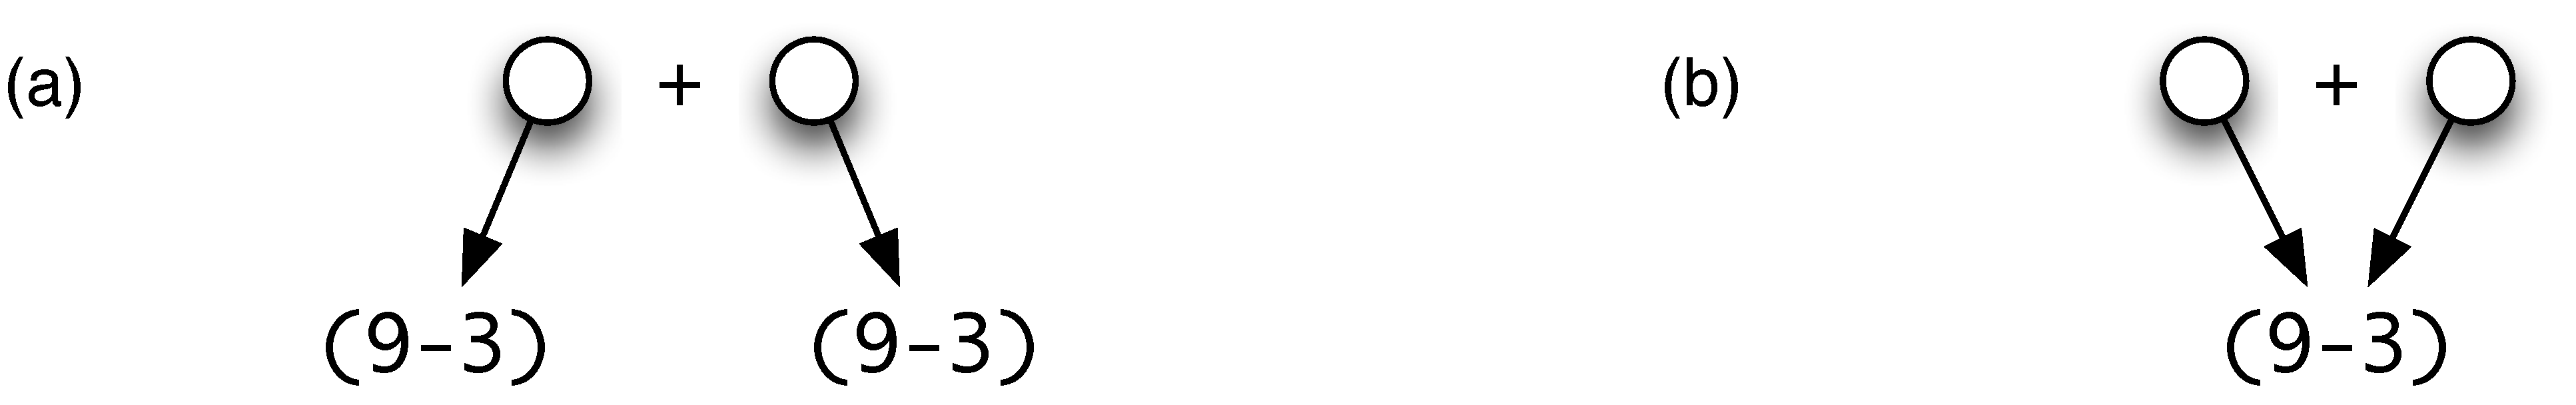
\includegraphics[width=4in]{Pictures/Sharing.pdf}
\end{center}
A final example is given by the pattern matching \index{pattern matching}
function,
\begin{alltt}
pm (x,y) = x+1
\end{alltt}
applied to the pair \texttt{(3+2,4-17)}. 
\begin{alltt}
pm (3+2,4-17)
\step (3+2)+1
\step 6
\end{alltt}
The argument is examined, and part of it is evaluated. The second
half of the pair remains unevaluated, as it is not needed in the calculation.
This completes the informal introduction to lazy evaluation, which can be
summarized in the three points:
\begin{titemize}
\item arguments to functions are evaluated only when this is necessary for
evaluation to continue;
\item an argument is not necessarily evaluated fully: only the parts that are
needed are examined;
\item an argument is evaluated at most only once. This is done in the
implementation by replacing expressions by graphs and calculating
over them.
\end{titemize}
We now give a more formal account of the calculation rules which embody lazy
evaluation.
\index{lazy evaluation|)}

\section{Calculation rules and lazy evaluation}
\label{calcRules}
\index{calculation!rules|(}

As we first saw in Section \ref{syntax}, the definition of a function
consists of a number of conditional
equations. Each conditional equation can contain multiple clauses 
and may have a number of local definitions given in a
\texttt{where} clause. Each equation will have on its left-hand side the function
under definition applied to a number of patterns.
\begin{alltt}
f \pone \ptwo ... \pk
  | \gone          = \eone
  | \gtwo          = \etwo
  ...
  | otherwise   = \er
    where
    \vone  \aoneone ... = \rone
    ....
f \qone \qtwo ... \qk
  = ...
\end{alltt}
In calculating \texttt{f \subscr{a}{1} \ldots\ \subscr{a}{k}} there are
three aspects. 

\subsection*{Calculation -- pattern matching}
\index{pattern matching!calculation}

In order to determine which of the equations is used, the arguments are
evaluated. The arguments are not evaluated fully, rather they are
evaluated sufficiently to see whether they match the corresponding patterns.
If they match the patterns \texttt{\subscr{p}{1}} to \texttt{\subscr{p}{k}},
then evaluation proceeds using the first equation; if not, they are checked
against the second equation, which may require further evaluation. This is
repeated until a match is given, or until there are no more equations (which would
generate a \texttt{Program  error}). For instance,
given the definition
\begin{alltt}
f :: [Int] -> [Int] -> Int
f [] ys         = 0 \hfill (f.1)
f (x:xs) []     = 0 \hfill (f.2)
f (x:xs) (y:ys) = x+y \hfill (f.3)
\end{alltt}
the evaluation of \texttt{f [1 ..\ 3] [1 ..\ 3]} proceeds thus
\begin{alltt}
f [1 ..\ 3] [1 ..\ 3]\hfill (1)
\step f (1:[2 ..\ 3]) [1 ..\ 3]\hfill (2)
\step f (1:[2 ..\ 3]) (1:[2 ..\ 3])\hfill (3)
\step 1+1\hfill (4)
\end{alltt}
At stage \texttt{(1)}, there is not enough information about the arguments to
determine whether there is a match with \texttt{(f.1)}. One step of evaluation
gives \texttt{(2)}, and shows there is not a match with \texttt{(f.1)}.

The first argument of \texttt{(2)} matches the first pattern of \texttt{(f.2)}, so
we need to check the second. One step of calculation in \texttt{(3)} shows that
there is no match with \texttt{(f.2)}, but that there is with \texttt{(f.3)}; hence we
have \texttt{(4)}.

\subsection*{Calculation -- guards}
\index{guard!calculation}

Suppose that the first conditional equation matches (simply for the sake of
explanation). The expressions
\texttt{\subscr{a}{1}} to \texttt{\subscr{a}{k}} are 
substituted for the patterns  \texttt{\subscr{p}{1}} to \texttt{\subscr{p}{k}}
throughout the conditional equation. We must next
determine which of the clauses on the right-hand side applies. The guards
are evaluated in turn, until one is found which gives the value 
\texttt{True}; the corresponding clause is then used. If we have
\begin{alltt}
f :: Int -> Int -> Int -> Int
f m n p
  | m>=n \&\& m>=p        = m
  | n>=m \&\& n>=p        = n
  | otherwise           = p
\end{alltt}
then
\begin{alltt}
f (2+3) (4-1) (3+9)
  ??  (2+3)>=(4-1) \&\& (2+3)>=(3+9)
  ??    \step 5>=3 \&\& 5>=(3+9)
  ??    \step True \&\& 5>=(3+9) 
  ??    \step 5>=(3+9)
  ??    \step 5>=12
  ??    \step False
  ??  3>=5 \&\& 3>=12
  ??    \step False \&\& 3>=12
  ??    \step False
  ??  otherwise \step True
\step 12
\end{alltt}
We leave it as an exercise for the reader to work out which parts of the
calculation above are shared.

\subsection*{Calculation -- local definitions}
\index{local definitions!calculation}

Values in \texttt{where} clauses are calculated on demand: only
when a value is needed does calculation begin. Given the definitions
\begin{alltt}
f :: Int -> Int -> Int

f m n
  | notNil xs    = front xs
  | otherwise    = n
    where
    xs = [m ..\ n]

front (x:y:zs) = x+y
front [x]      = x

notNil []    = False
notNil (_:_) = True
\end{alltt}
the calculation of \texttt{f 3 5} will be
\begin{alltt}
f 3 5
  ?? notNil xs
  ??     where 
  ??     xs = [3 ..\ 5]
  ??\vertline{30pt}       \step 3:[4 ..\ 5] \hfill (1)
  ?? \step notNil (3:[4 ..\ 5])
  ?? \step True
\step front xs
       where
       xs = 3:[4 ..\ 5]
\vertline{30pt}          \step 3:4:[5] \hfill (2)
\step 3+4\hfill (3)
\step 7
\end{alltt}
To evaluate the guard \texttt{notNil xs}, evaluation of \texttt{xs} begins, and after
one step, \texttt{(1)} shows that the guard is \texttt{True}. Evaluating \texttt{front
xs} requires more information about \texttt{xs}, and so we evaluate by one more
step to give \texttt{(2)}. A successful pattern match in the definition of 
\texttt{front} then gives \texttt{(3)}, and so the result.

This section has described \texttt{where} clauses; a similar explanation applies to \texttt{let} expressions.

\subsection*{Operators and other expression formers}
\index{operator!calculation}

The three aspects of evaluating a function application are now complete; we
should now say something about the built-in operators. If they can be given
Haskell definitions, such as
\begin{alltt}
True  \&\& x = x\index{\&@\texttt{\&}}
False \&\& x = False
\end{alltt}
then they will follow the rules for Haskell definitions. The left-to-right
order means that `\texttt{\&\&}' will not evaluate its second argument in the case that its
first is \texttt{False}, for instance. This is unlike many programming languages, where
the `and' function will evaluate both its arguments.

The other operations, such as the
arithmetic operators, vary. Multiplication \minx{*} needs both its arguments
to return a result\footnote{In fact, multiplication could be `lazier', since it is possible to say that \texttt{0*n} is \texttt{0} without evaluating \texttt{n}.} but the equality \index{equality}
on lists can return \texttt{False} on
comparing \texttt{[]} and \texttt{(x:xs)} without evaluating \texttt{x} or \texttt{xs}. In
general the language is implemented so that no manifestly
unnecessary evaluation takes
place.

Recall that \texttt{if} \ldots \texttt{then} \ldots \texttt{else} \ldots;
\texttt{cases}; \texttt{let} and lambda
expressions can be used in forming expressions. Their evaluation follows the
form we have seen for function applications. Specifically, 
\texttt{if} \ldots \texttt{then} \ldots \texttt{else} \ldots
\ is evaluated like a guard, \texttt{cases} like a pattern match, 
\texttt{let} like a \texttt{where} clause and a lambda expression like the application of
a named function such as \texttt{f} above.

Finally, we turn to the way in which a choice is made between applications.
              
\subsection*{Evaluation order}
\index{evaluation order}

What characterizes evaluation in Haskell, apart from the fact that no argument
is evaluated more than once, is the \textbf{order} in which applications are evaluated
when there is a choice.
\begin{titemize}
\item Evaluation is \textbf{from the outside in}. In a situation like
\begin{alltt}
\underline{\subscr{f}{1} \eone\ \underline{(\subscr{f}{2} \etwo\ 17)}}
\end{alltt}
where one application encloses another, the outer one is evaluated. In the example, the outer one, \texttt{\subscr{f}{1}~\eone~(\subscr{f}{2} \etwo\ 17)}, is
chosen for evaluation. 
\item Otherwise, evaluation is \textbf{from left to right}.
In the expression
\begin{alltt}
\underline{\subscr{f}{1} \eone} + \underline{\subscr{f}{2} \etwo}
\end{alltt}
the underlined expressions are both to be evaluated. The left-hand one, 
\texttt{\subscr{f}{1} \eone}, will be evaluated first.
\end{titemize}
These rules are enough to describe the way in which lazy evaluation works. In
the sections to come we look at the consequences of a lazy approach for
functional programming.

\index{calculation!rules|)}

\section{List comprehensions revisited}
\label{listCompRev}
\index{list comprehensions|(}

The list comprehension notation does not add any new programs to the
Haskell language, but it does allow us to (re-)write programs in a new and
clearer way. Building on the introduction in Section \ref{listComps}, the
notation lets us combine multiple \texttt{map}s and \texttt{filter}s together in a
single expression. Combinations of these functions
allow us to write algorithms which generate and test: all the elements
of a particular form are generated and  combinations of them are tested, before
results depending upon them are returned. 

We begin the section with a
re-examination of the syntax of the list comprehension, before giving some
simple examples to illustrate the features that we describe. After that we give the rules for calculating
with list comprehensions, and we finish the section with a series of longer
examples.

\subsection*{Syntax}
\index{list comprehensions!syntax}

A list comprehension has the form
\begin{alltt}
[ e | \subscr{q}{1} , \ldots\ , \subscr{q}{k} ]
\end{alltt}
where each \textbf{qualifier}\index{qualifier} \texttt{\subscr{q}{i}} has one of two forms.
\begin{titemize}
\item It can be a \textbf{generator}, \index{list comprehensions!generator}
\texttt{p <- lExp},
where \texttt{p} %each \texttt{\subscr{p}{j}} 
is a pattern and \texttt{lExp} is an
expression of list type.
\item It can be a \textbf{test}, \texttt{bExp}, \index{list comprehensions!test}
which is a boolean expression.
\end{titemize}
An expression \texttt{lExp} or \texttt{bExp} appearing in qualifier 
\texttt{\subscr{q}{i}} can refer to the
variables used in the patterns of qualifiers \texttt{\subscr{q}{1}} to 
\texttt{\subscr{q}{i-1}}.

\subsection*{Simpler examples}

Multiple generators \index{list comprehensions!multiple generators}
allow us to combine elements from two or more lists
\begin{alltt}
pairs :: [a] -> [b] -> [(a,b)]
pairs xs ys = [ (x,y) | x<-xs , y<-ys ]
\end{alltt}
This example is important as it shows the way in which the values \texttt{x} and
\texttt{y} are chosen.
\begin{alltt}
pairs [1,2,3] [4,5] 
\step [(1,4),(1,5),(2,4),(2,5),(3,4),(3,5)]
\end{alltt}
The first element of \texttt{xs}, \texttt{1}, is given to \texttt{x}, and then {\em for
this fixed value\/} all possible values of \texttt{y} in \texttt{ys} are chosen. This
process is repeated for the remaining values \texttt{x} in \texttt{xs}, namely 
\texttt{2} and \texttt{3}. 

This choice is not accidental, since if we have
\begin{alltt}
triangle :: Int -> [(Int,Int)]\minx{triangle}
triangle n = [ (x,y) | x <- [1 ..\ n] , y <- [1 ..\ x] ]
\end{alltt}
the second generator, \texttt{y <- [1 ..\ x]} depends on the value of \texttt{x} given
by the first generator.
\begin{alltt}
triangle 3 
\step [(1,1),(2,1),(2,2),(3,1),(3,2),(3,3)]
\end{alltt}
For the first choice of \texttt{x}, \texttt{1}, the value of \texttt{y} is 
chosen from \texttt{[1 ..\ 1]},
for the second choice of \texttt{x}, the value of \texttt{y} is chosen from 
\texttt{[1 ..\ 2]}, and so on.

Three positive integers form a \emph{Pythagorean 
triple}\index{Pythagorean triple} if the sum of squares of the first 
two is equal to the square of the third. The list of all triples with all sides
below a
particular bound, \texttt{n}, is given by
\begin{alltt}\minx{pyTriple}
pyTriple n
  = [ (x,y,z) | x <- [2 ..\ n] , y <- [x+1 ..\ n] , 
                z <- [y+1 ..\ n] , x*x + y*y == z*z ]

pyTriple 100 
\step [(3,4,5),(5,12,13),(6,8,10),...,(65,72,97)]         
\end{alltt}
Here the test combines values from the three generators.



\subsection*{Calculating with list comprehensions}
\index{list comprehensions!calculation rules}

How can we describe the way in which the results of list comprehensions are
obtained? One way is to give a translation of the comprehensions into
applications of \texttt{map}, \texttt{filter} and \texttt{concat}.
We give a different approach here, of calculating {\em directly\/} with the
expressions. 

Before we do this, we introduce one piece of very helpful notation. We write
\texttt{e\{f/x\}} \index{substitution}
for the expression \texttt{e} in which every occurrence of the
variable \texttt{x} has been replaced by the expression \texttt{f}. This is the
\textbf{substitution} of \texttt{f} for \texttt{x} in \texttt{e}. If \texttt{p} is a
pattern, we use  \texttt{e\{f/p\}} for the substitution of the appropriate parts
of \texttt{f} for the variables in \texttt{p}. For instance,
\begin{alltt}
[ (x,y) | x<-xs ]\{[2,3]/xs\}    = [ (x,y) | x<-[2,3] ]

(x + sum xs)\{(2,[3,4])/(x,xs)\} = 2 + sum [3,4]
\end{alltt} 
since \texttt{2} matches \texttt{x}, and \texttt{[3,4]} matches \texttt{xs} when 
\texttt{(2,[3,4])} is matched against \texttt{(x,xs)}.

We now explain list comprehensions. The notation looks a bit daunting,
but the effect should be clear. The generator \texttt{v <-
[\subscr{a}{1},...,\subscr{a}{n}]} has the effect of setting \texttt{v} to the
values \texttt{\subscr{a}{1}} to \texttt{\subscr{a}{n}} in turn. Setting the value
appears in the calculation as \textbf{substitution} of a value for a variable. 
\begin{alltt}
[ e | v <- [\subscr{a}{1},...,\subscr{a}{n}] , \subscr{q}{2} , \ldots\ , \subscr{q}{k} ]  
\step [ e\{\subscr{a}{1}/v\} | \subscr{q}{2}\{\subscr{a}{1}/v\} , \ldots\ , \subscr{q}{k}\{\subscr{a}{1}/v\} ] 
    ++ ... ++
    [ e\{\subscr{a}{n}/v\} | \subscr{q}{2}\{\subscr{a}{n}/v\} , \ldots\ , \subscr{q}{k}\{\subscr{a}{n}/v\} ] 
\end{alltt}
As a running example for this section we take 
\begin{alltt}
[ x+y | x <- [1,2] , isEven x , y <- [x ..\ 2*x] ]
\step [ 1+y | isEven 1 , y <- [1 ..\ 2*1] ] ++
    [ 2+y | isEven 2 , y <- [2 ..\ 2*2] ]
\end{alltt} 
where the values \texttt{1} and \texttt{2} are substituted for \texttt{x}.
The rules for tests are simple,
\begin{alltt}
[ e | True  , \subscr{q}{2} , \ldots\ , \subscr{q}{k} ] 
\step [ e | \subscr{q}{2} , \ldots\ , \subscr{q}{k} ]

[ e | False , \subscr{q}{2} , \ldots\ , \subscr{q}{k} ] 
\step []
\end{alltt}
so that our example is
\begin{alltt}
\step [ 1+y | False , y <- [1 ..\ 2*1] ] ++
    [ 2+y | True , y <- [2 ..\ 2*2] ]
\step [ 2+y | y <- [2,3,4] ]
\step [ 2+2 | ] ++ [ 2+3 | ] ++ [ 2+4 | ]
\end{alltt}
and when there are no qualifiers,
\begin{alltt}
[ e | ] = [ e ]
\end{alltt}
Completing the example, we have
\begin{alltt}
[ x+y | x <- [1,2] , isEven x , y <- [x ..\ 2*x] ] 
\step [4,5,6]
\end{alltt}
Now we consider some more examples.
\begin{alltt}
triangle 3
\step [ (x,y) | x <- [1 ..\ 3] , y <- [1 ..\ x] ]
\step [ (1,y) | y <- [1 ..\ 1] ] ++ 
    [ (2,y) | y <- [1 ..\ 2] ] ++
    [ (3,y) | y <- [1 ..\ 3] ]
\step [ (1,1) | ] ++ 
    [ (2,1) | ] ++ [ (2,2) | ] ++
    [ (3,1) | ] ++ [ (3,2) | ] ++ [ (3,3) | ]
\step [(1,1),(2,1),(2,2),(3,1),(3,2),(3,3)]
\end{alltt}
as we argued above. Another example contains a test:
\begin{alltt}
[ m*m | m <- [1 ..\ 10] , m*m<50 ]
\step [ 1*1 | 1*1<50 ] ++ [ 2*2 | 2*2<50 ] ++ ...
    [ 7*7 | 7*7<50 ] ++ [ 8*8 | 8*8<50 ] ++ ...
\step [ 1  | True ] ++ [ 4  | True ] ++ ...
    [ 49 | True ] ++ [ 64 | False ] ++ ...
\step [1,4,...49]
\end{alltt}
We now look at two longer examples, the  solutions for which are aided by the list
comprehension style.
%\pagebreak
\subsection*{Example}
\subsubsection*{List permutations}
\index{lists!permutations}

A permutation of a list is a list with the 
same elements in a different order. For a list of \texttt{n} elements, there are \texttt{n\ensuremath{!}} (\texttt{n} factorial) permutations of the list. The \texttt{perms} function returns a list
of all permutations of a list.\minx{perms}
\begin{alltt} 
perms :: Eq a => [a] -> [[a]]
\end{alltt}
The empty list has one permutation, 
itself. If \texttt{xs} is not empty, a permutation is given by 
picking an element \texttt{x} from \texttt{xs} and 
putting \texttt{x} at the front of a permutation of the 
remainder \texttt{xs} with \texttt{x} removed. To do this we use the `\texttt{\bs{}\bs{}}' operator, defined in \texttt{Data.List}.

The operator `\texttt{\bs{}\bs{}}' returns the difference of
two lists: \texttt{xs\bs{}\bs{}ys} is the list \texttt{xs} with each element of \texttt{ys}
removed, if it is present. The number of duplications is taken into account, so that for  example \texttt{[2,3,2]\bs{}\bs{}[3,2,3]} is \texttt{[2]}. We can now write the definition of the function giving all the permutations like this
\begin{alltt}
perms [] = [[]]
perms xs = [ x:ps | x <- xs , ps <- perms (xs\bs{}\bs{}[x]) ]
\end{alltt}
Example evaluations give, for a one-element list,
\begin{alltt}
perms [2]
\step [x:ps| x <- [2] , ps <- perms [] ] 
\step [x:ps| x <- [2] , ps <- [[]] ] 
\step [2:ps| ps <- [[]] ] 
\step [2:[] | ]
\step [[2]]
\end{alltt}
for a two-element list,
\begin{alltt}
perms [2,3]
\step [ x:ps | x <- [2,3] , ps <- perms([2,3]\bs{}\bs{}[x]) ]
\step [ 2:ps | ps <- perms [3] ] ++ [ 3:ps | ps <- perms [2] ]
\step [ 2:[3] ] ++ [ 3:[2] ]
\step [ [2,3] , [3,2] ]
\end{alltt}
and finally for a three-element list,
\begin{alltt}
perms [1,2,3]
\step [ x:ps | x <- [1,2,3] , ps <- perms([1,2,3]\bs{}\bs{}[x]) ]
\step [ 1:ps | ps <- perms [2,3]] ++...++ [ 3:ps | ps <- perms [1,2]]
\step [ 1:ps | ps<-[[2,3],[3,2]]] ++...++ [ 3:ps | ps<-[[1,2],[2,1]]]
\step [[1,2,3],[1,3,2],[2,1,3],[2,3,1],[3,1,2],[3,2,1]]
\end{alltt}
There is another algorithm for permutations: in this, a permutation of a
list \texttt{(x:xs)} is given by forming a 
permutation of \texttt{xs}, and by inserting \texttt{x} into this somewhere. The
possible insertion points are given by finding all the possible {\em splits\/}
of the list into two halves.\minx{perm}
\begin{alltt}
perm :: [a] -> [[a]]

perm []     = [[]]
perm (x:xs) = [ ps++[x]++qs | rs <- perm xs ,
                              (ps,qs) <- splits rs ]
\end{alltt}
We get the list of all possible \texttt{splits} of a list \texttt{xs} after seeing
that on splitting \texttt{(y:ys)}, we either split at the front of \texttt{(y:ys)}, or
somewhere inside \texttt{ys}, as given by a split of \texttt{ys}.
\begin{alltt}
splits :: [a]->[([a],[a])]

splits []     = [ ([],[]) ]
splits (y:ys) = ([],y:ys) : [ (y:ps,qs) | (ps,qs) <- splits ys]
\end{alltt}
Before moving on, observe that the type of \texttt{perms} requires that
\texttt{a} must be in the class \texttt{Eq}.
This is needed for the list difference operator \texttt{\bs{}\bs{}}
to be defined over the type
\texttt{[a]}. There is no such restriction on the type of \texttt{perm}, which
uses a different method for calculating the permutations.


\subsection*{Vectors and matrices}

In this section we give one model for vectors and matrices of real numbers;
others exist, and are suitable for different purposes. In particular, the \texttt{Data.Array}\minx{Data.Array} package provides implementations of both immutable and mutable arrays: the former are `functional', and so can only be updated by copying,  while the latter can be updated `in place'.

In our implementation, a vector is a list of real numbers, as in the example vector \texttt{[2.1,3.0,4.0]}. 
\begin{alltt}
type Vector = [Float]\minx{Vector}
\end{alltt}
The scalar product of
two vectors (assumed to be the same length) is given by multiplying together
corresponding elements and taking the total of the results.
\begin{alltt}
scalarProduct [2.0,3.1] [4.1,5.0] 
\step 2.0*4.1 + 3.1*5.0 
\step 23.7
\end{alltt}
As a first attempt we might write
\begin{alltt}
mul xs ys = sum [ x*y | x<-xs , y<-ys ]
\end{alltt}
but this gives
\begin{alltt}
mul [2.0,3.1] [4.1,5.0] 
\step sum [8.2,10.0,12.71,15.5] 
\step 46.41
\end{alltt}
since {\em all\/} combinations of pairs from the lists are taken. In order to
multiply together corresponding pairs, we first \texttt{zip} 
the lists together:
\begin{alltt}\minx{scalarProduct}
scalarProduct :: Vector -> Vector -> Float
scalarProduct xs ys = sum [ x*y | (x,y) <- zip xs ys ]
\end{alltt}
and a calculation shows that this gives the required result. It is also
possible to use \texttt{zipWith} to define \texttt{scalarProduct}; we leave this as an exercise. A matrix like
\[ 
\left( \begin{array}{rrr} 2.0 & 3.0 & 4.0 \\ 5.0 & 6.0 & -1.0 \end{array} \right)
\]
can be
thought of as a list of rows or a list of columns; we choose a list of rows
here.
\begin{alltt}
type Matrix = [Vector]\minx{Matrix}
\end{alltt}
The example matrix is 
\begin{alltt}
[[2.0,3.0,4.0],[5.0,6.0,-1.0]]
\end{alltt}
Two matrices \texttt{M} and 
\texttt{P} are multiplied by taking the scalar products of rows of \texttt{M} with
columns of \texttt{P}.
\[ 
\left( \begin{array}{rrr} 2.0 & 3.0 & 4.0 \\ 5.0 & 6.0 & -1.0 \end{array} \right)
\times
\left( \begin{array}{rr} 1.0 & 0.0 \\ 1.0 & 1.0 \\ 0.0 & -1.0 \end{array} \right)
= 
\left( \begin{array}{rr} 5.0 & -1.0 \\ 11.0 & 7.0 \end{array} \right)
\]
We therefore define
\begin{alltt}\minx{matrixProduct}
matrixProduct :: Matrix -> Matrix -> Matrix
matrixProduct m p
  = [ [scalarProduct r c | c <- columns p] | r <- m ]
\end{alltt}
where the function \texttt{columns} gives the representation of a matrix as a
list of columns.
\begin{alltt}
columns :: Matrix -> Matrix

columns y = [ [ z!!j | z <- y ] | j <- [0 ..\ s] ]
            where 
            s = length (head y)-1
\end{alltt}
The expression \texttt{[ z!!j | z <- y ]} picks the \texttt{j}th element from 
each row \texttt{z} in \texttt{y}; this is exactly the \texttt{j}th 
column of \texttt{y}. \texttt{length (head y)}
is the length of a row in \texttt{y}, and so
the indices \texttt{j} will be in the range \texttt{0} to \texttt{s =
length (head y)-1}. Another variant of the \texttt{columns} function is
\texttt{transpose} which is in the library \texttt{Data.List}.

\subsubsection*{Refutable patterns in generators}
\index{list comprehensions!refutable patterns}
\index{pattern!refutable}

Some patterns are \textbf{refutable}, meaning that
an attempt to pattern-match against them may fail. If a refutable pattern is
used on the left-hand side of an `\texttt{<-}', its effect is to filter from the
list only the elements matching the pattern. For example,
\begin{alltt}
[ x | (x:xs) <- [[],[2],[],[4,5]] ] \step [2,4]
\end{alltt}
The rules for calculation with generators containing a refutable pattern on
their left-hand side are similar to those given above,
except that before performing the
substitution for the pattern, the list is filtered for the elements which
match the pattern. The details are left as an exercise.

\begin{exercises}

\item
Give a calculation of the expression
\begin{alltt}
[ x+y | x <- [1 ..\ 4] , y <- [2 ..\ 4] , x>y ]
\end{alltt}

\item
Using the list comprehension notation, define the functions 
\begin{alltt}
subLists,subSequences :: [a] -> [[a]]
\end{alltt}
which return all the
sublists and subsequences of a list. A sublist is obtained by omitting some
of the elements of a list; a subsequence is a
continuous block from a list. For instance, both \texttt{[2,4]} and \texttt{[3,4]}
are sublists of \texttt{[2,3,4]}, but only \texttt{[3,4]} is a subsequence.

\item
Give calculations of the expressions
\begin{alltt}
perm [2]
perm [2,3]
perm [1,2,3]
\end{alltt}
and of the matrix multiplication
\begin{alltt}
matrixProduct [[2.0,3.0,4.0],[5.0,6.0,-1.0]] 
              [[1.0,0.0],[1.0,1.0],[0.0,-1.0]]
\end{alltt}

\item
Give a definition of \texttt{scalarProduct} using \texttt{zipWith}.

\item
Define functions to calculate
the determinant of a square matrix and, if this is
non-zero, to invert the matrix.

\item
The calculation rules for list comprehensions can be re-stated for the two
cases \texttt{[]} and \texttt{(x:xs)}, instead of for the arbitrary list 
\texttt{[\subscr{a}{1},...,\subscr{a}{n}]}.
Give these rules by completing the equations
\begin{alltt}
[ e | v <- []     , \subscr{q}{2} , \ldots\ , \subscr{q}{k} ] \step ...
[ e | v <- (x:xs) , \subscr{q}{2} , \ldots\ , \subscr{q}{k} ] \step ...
\end{alltt}

\item
Give the precise rules for calculating with a generator containing a refutable 
pattern,
like \texttt{(x:xs) <- lExp}. You might need to define auxiliary functions to do
this.

\item
List comprehensions can be translated into expressions involving \texttt{map},
\texttt{filter} and \texttt{concat} by the following equations.
\begin{alltt}
[ x | x<-xs ]              = xs
[ f x | x<-xs ]            = map f xs
[ e | x<-xs , p x , ... ]  = [ e | x <- filter p xs , ... ]
[ e | x<-xs , y<-ys , .. ] = concat [ [e|y<-ys, ..] | x<-xs]
\end{alltt}
Translate the expressions
\begin{alltt}
[ m*m | m <- [1 ..\ 10] ]
[ m*m | m <- [1 ..\ 10] , m*m<50 ]
[ x+y | x <- [1 ..\ 4] , y <- [2 ..\ 4] , x>y ]
[ x:p | x <- xs , p <- perms (xs\bs{}\bs{}[x]) ]
\end{alltt}
using these equations; you will need to define some auxiliary functions as a
part of your translation.

\index{list comprehensions|)}

\end{exercises}


\section{Data-directed programming}
\index{data-directed programming|(}
\index{design!data-directed}

This section looks at style of programming made possible by lazy evaluation,
\textbf{data-directed programming}. This is an approach where we design the program by thinking about it as a sequence of transformations of data.  

`In a traditional language it may well be too efficient to do this in practice, as we might have to compute a series of complex data structures which are `internal' to the program. In a lazy language these are only constructed as they are needed, and in practice they may never be constructed completely: we just build the data structures incrementally, and once a part of it has been used, it can be `recycled'. Luckily this is done by the implementation, and we do not have to worry about it ourselves. 


All this should become clearer as we look at a particular example; let's start by looking at the example of finding the sum
of fourth powers of numbers from \texttt{1} to \texttt{n}. A data-directed
solution is to
\begin{titemize}
\item build the list of numbers \texttt{[1 ..\ n]};
\item take the power of each number, giving 
\texttt{[1,16,\ldots,\superscr{n}{4}]}, and
\item find the sum of this list.
\end{titemize}
As a program, we have
\begin{alltt}
sumFourthPowers n = sum (map (\^{}4) [1 ..\ n])
\end{alltt}
How does the calculation proceed?
\begin{alltt}
sumFourthPowers n 
\step sum (map (\^{}4) [1 ..\ n])
\ \hfill \mbox{\textrm{create first part of the list with \texttt{:}}}
\step sum (map (\^{}4) (1:[2 ..\ n]))\hfill \mbox{\textrm{allows pattern match}}
\step sum (1\^{}4 : map (\^{}4) [2 ..\ n])\hfill \mbox{\textrm{by definition of \texttt{map}}}
\step (1\^{}4) + sum (map (\^{}4) [2 ..\ n]) \hfill \mbox{\textrm{by definition of \texttt{sum}}}
\ \ \hfill \mbox{\textrm{now we can recycle the first part of the list}}
\step 1 + sum (map (\^{}4) [2 ..\ n]) 
\step ...
\step 1 + (16 + sum (map (\^{}4) [3 ..\ n])) 
\step ...
\step 1 + (16 + (81 + ... + \superscr{n}{4})) 
\end{alltt}
As can be seen, none of the intermediate lists is created in full in this
calculation. As soon as the first part of the list is created, its fourth power is
taken, and it becomes a part of the sum which produces the final result, and so the first part can be recycled.


\begin{example}

\subsubexample*{1. List minimum}
\index{lists!minimum of}

A more striking example is given by the problem of finding the minimum of a
list of numbers. One solution is to sort the list, and take its head! This
would be ridiculous if the whole list were sorted in the process, but, in
fact we have, using the definition of insertion sort from
Chapter \ref{defFunLists},
\begin{alltt}
iSort [8,6,1,7,5]\minx{iSort}\minx{ins}
\step ins 8 (ins 6 (ins 1 (ins 7 (ins 5 []))))
\step ins 8 (ins 6 (ins 1 (ins 7 \underline{[5]}))) 
\step ins 8 (ins 6 (ins 1 \underline{(5 : ins 7 [])}))
\step ins 8 (ins 6 \underline{(1 : (5 : ins 7 []))})
\step ins 8 \underline{(1 : ins 6 (5 : ins 7 []))}
\step \underline{1 : ins 8 (ins 6 (5 : ins 7 []))}
\end{alltt}
As can be seen from the underlined parts of the calculation, each application
of \texttt{ins} calculates the minimum of a larger part of the list, since the
head of the result of \texttt{ins} is given in a single step. The head of the
whole list is determined in this case without us working out the value of the
tail, and this means that we have a sensible algorithm for minimum given by
\texttt{(head .\ iSort)}.

\subsubexample*{2. Routes through a graph}
\index{graph!routes through}

A graph can be seen as an object of type \texttt{Relation a}\minx{Relation},
as defined in
Section \ref{rels}. How can we find a route from one point in a graph to
another? For example, in the graph
\begin{center}
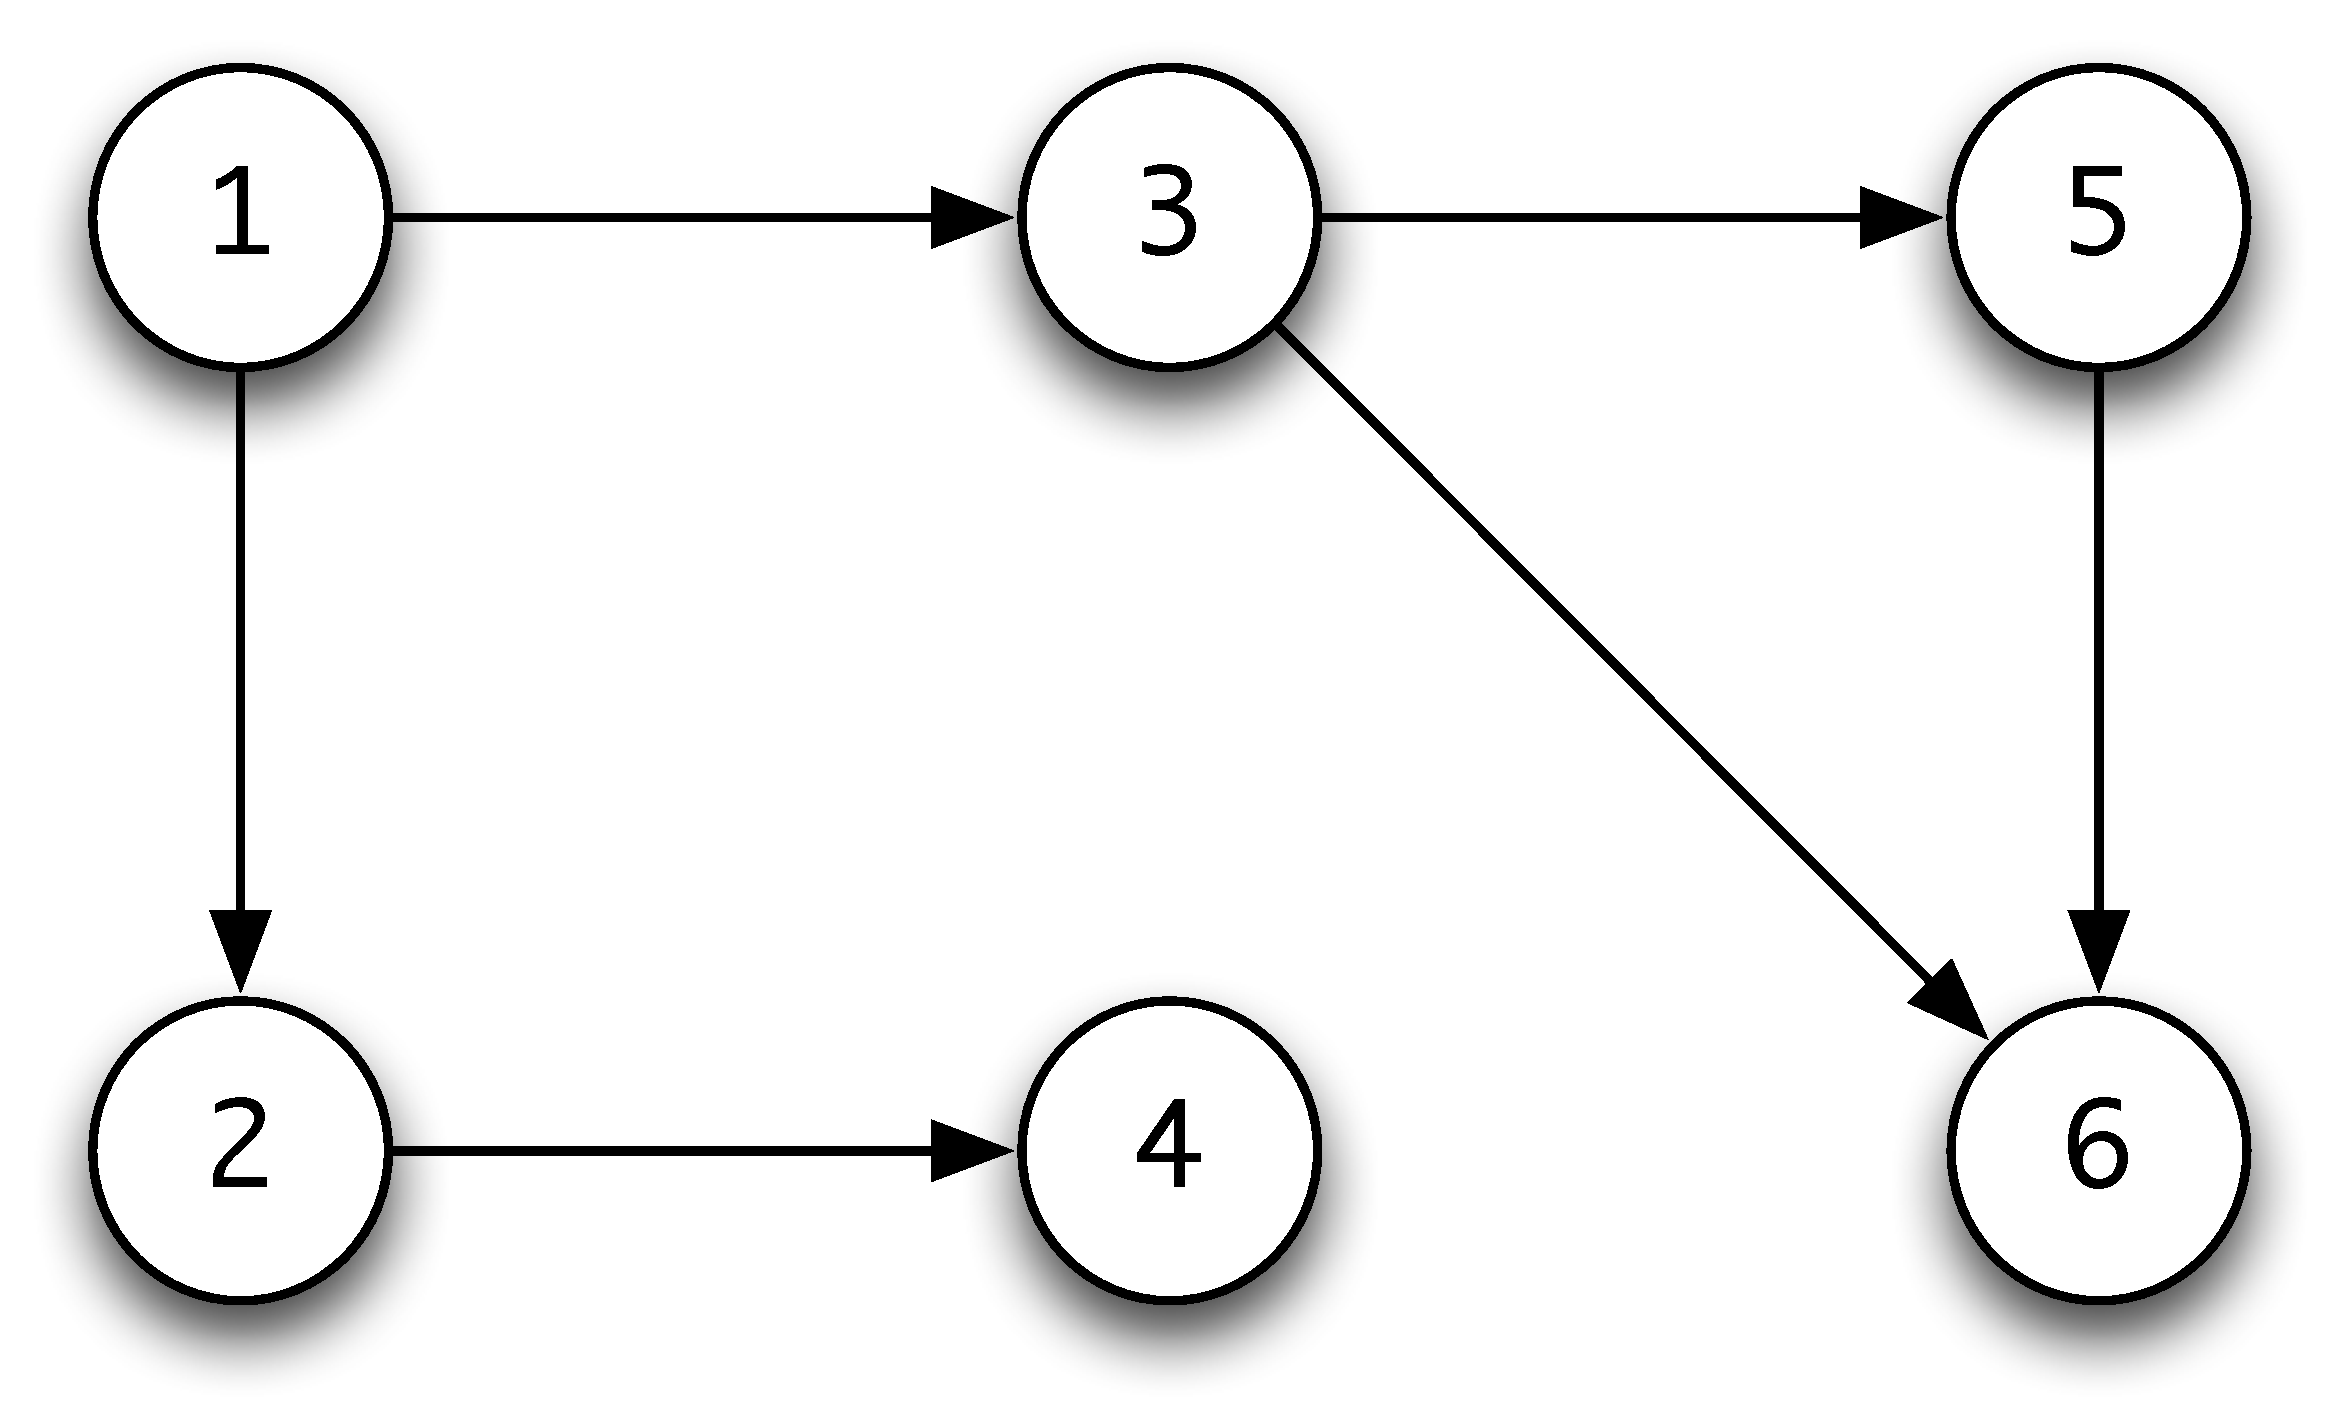
\includegraphics[width=2in]{Pictures/Graph2.pdf}
\end{center} 
\begin{alltt}
graphEx = makeSet [(1,2),(1,3),(2,4),(3,5),(5,6),(3,6)]
\end{alltt}
a route from \texttt{1} to \texttt{4} is the list \texttt{[1,2,4]}. 

We solve a
slightly different problem: find the list of {\em all\/} routes from \texttt{x} to
\texttt{y}; our original problem is solved by taking the head of this list. Note
that as a list is returned, the algorithm allows for the possibility of there
being {\em no\/} route from \texttt{x} to \texttt{y} -- the empty list of routes is
the answer in such a case. This method, which is applicable in many different
situations, is often called the \textbf{list of successes}
\index{list of successes method}
technique: instead of
returning one result, or an error if there is none, we return a list; the
error case is signalled by the empty list. The method also allows for multiple
results to be returned, as we shall see.

How do we solve the new problem? 


\paragraph{Acyclic case.}

For the present
we assume that the graph is \textbf{acyclic}: there is no circular path from
any node back to itself.

\begin{titemize} 
\item The only route from \texttt{x} to \texttt{x} is \texttt{[x]}.
\item A route from \texttt{x} to \texttt{y} will start with a step to one of 
\texttt{x}'s neighbours, \texttt{z} say. The remainder will be a path from
\texttt{z} to \texttt{y}.
\end{titemize}
We therefore look for all paths from \texttt{x} to \texttt{y} going through 
\texttt{z}, for each neighbour \texttt{z} of \texttt{x}.
\begin{alltt}\minx{routes}
routes :: Ord a => Relation a -> a -> a -> [[a]]
routes rel x y
  | x==y        = [[x]]
  | otherwise   = [ x:r | z <- nbhrs rel x ,
                          r <- routes rel z y ]
\end{alltt}
The \texttt{nbhrs} function is defined by
\begin{alltt}\minx{nbhrs}
nbhrs :: Ord a => Relation a -> a -> [a]
nbhrs rel x = flatten (image rel x)
\end{alltt} 
where \texttt{flatten} turns a set into a list.
Now consider the example, where we write \texttt{routes'} for \texttt{routes
graphEx} and \texttt{nbhrs'} for \texttt{nbhrs graphEx},
to make the calculation more readable:
\begin{alltt}
routes' 1 4
\step [ 1:r | z <- nbhrs' 1 , r <- routes' z 4 ]
\step [ 1:r | z <- [2,3] , r <- routes' z 4 ]
\step [ 1:r | r <- routes' 2 4 ] ++ 
    [ 1:r | r <- routes' 3 4 ]\hfill (\dag)
\step [ 1:r | r <- [ 2:s | w <- nbhrs' 2 , s <- routes' w 4 ]]++...
\step [ 1:r | r <- [ 2:s | w <- [4] , s <- routes' w 4 ] ] ++ ...
\step [ 1:r | r <- [ 2:s | s <- routes' 4 4 ] ] ++ ...\hfill (\ddag)
\step [ 1:r | r <- [ 2:s | s <- [[4]] ] ] ++ ...
\step [ 1:r | r <- [ [2,4] ] ] ++ ...
\step [[1,2,4]] ++ ...
\end{alltt}
The head of the list is given by exploring only the first neighbour of 
\texttt{1}, namely \texttt{2}, and its first neighbour, \texttt{4}. In this case 
the search
for a route leads directly to a result. This is not always so. Take the
example of
\begin{alltt}
routes' 1 6 = ...
\step [ 1:r | r <- routes' 2 6 ] ++ 
    [ 1:r | r <- routes' 3 6 ]\hfill (\dag)
\step ...
\step [ 1:r | r <- [ 2:s | s <- routes' 4 6 ] ] ++ 
    [ 1:r | r <- routes' 3 6 ]\hfill (\ddag)
\end{alltt}
Corresponding points in the calculations are marked by \texttt{(\dag)} and
\texttt{(\ddag)}. The search for routes from \texttt{4} to \texttt{6} will {\em fail\/},
though, as \texttt{4} has no neighbours -- we therefore have
\begin{alltt}
\step [] ++ [ 1:r | r <- routes' 3 6 ] = ...
\step [ 1:r | r <- [ 3:s | s <- routes' 5 6 ] ] ++ ...
\step [[1,3,5,6]] ++ ...
\end{alltt}
The effect of this algorithm is to \textbf{backtrack} \index{backtracking}
when a search has
failed: there is no route from \texttt{1} to \texttt{6} via \texttt{2}, so the other
possibility of going through \texttt{3} is explored. This is done  {\em only\/}
when the first possibility is exhausted, however, so lazy evaluation ensures
that this search through `all' the paths turns out to be an efficient method
of finding a single path. Moreover, we don't have to think explicitly about backtracking, it simply falls out from our description of the list of all solutions, evaluated lazily.


\paragraph{General case.}

We assumed at the start of this development that the graph was acyclic, so
that we have no chance of a path looping back on itself, and so of a search
going into a loop. We can make a simple addition to the program to make sure
that only paths without cycles are explored, and so that the program will
work for an arbitrary graph. We add a list argument for the points not to be
visited (again), and so have
\begin{alltt}\minx{routesC}
routesC :: Ord a => Relation a -> a -> a -> [a] -> [[a]]
routesC rel x y avoid
  | x==y        = [[x]]
  | otherwise   = [ x:r | z <- nbhrs rel x \bs{}\bs{} avoid ,
                          r <- routesC rel z y (x:avoid) ]
\end{alltt}
Two changes are made in the recursive case.
\begin{titemize}
\item In looking for neighbours of \texttt{x} we look only for those which are
not in the list \texttt{avoid};
\item in looking for routes from \texttt{z} to \texttt{y}, we exclude visiting both
the elements of \texttt{avoid} and the node \texttt{x} itself. 
\end{titemize}
A search for a route from \texttt{x} to \texttt{y} in \texttt{rel} is given by \texttt{
routesC rel x y []}.
\end{example}

\begin{exerciseone}
\item
Defining \texttt{graphEx2} to be
\begin{alltt} 
makeSet [(1,2),(2,1),(1,3),(2,4),(3,5),(5,6),(3,6)]
\end{alltt}
try calculating
the effect of the original definition on  
\begin{alltt}
routes graphEx 1 4
\end{alltt}
Repeat the calculation with the revised definition which follows:
\begin{alltt}
routes rel x y
  | x==y        = [[x]]   
  | otherwise   = [ x:r | z <- nbhrs rel x ,
                          r <- routes rel z y ,
                          not (elem x r) ]
\end{alltt}
and explain why this definition is not suitable for use on cyclic graphs.
Finally, give a calculation of 
\begin{alltt}
routesC graphEx 1 4 []
\end{alltt}
\index{data-directed programming|)}
\end{exerciseone}


\section{Case study: parsing expressions}
\label{parsing}
\index{case studies!parsing|see{parsing}}
\index{parsing|(}
\index{calculator|(}

We have already seen the definition of \texttt{Expr}, the type of arithmetic
expressions, in Section \ref{recTypes} and in a 
revised version given on page \pageref{modExpr}:
\begin{alltt}
data Expr = Lit Int | Var Var | Op Ops Expr Expr\minx{Expr}
data Ops  = Add | Sub | Mul | Div | Mod\minx{Ops}
\end{alltt}
and showed there how we could calculate
the results of these expressions using the function \texttt{eval}. Chapter
\minx{eval}\minx{Store}
\ref{adt} began with a discussion of how to represent the values held in the
variables using the abstract data type \texttt{Store}. Using these components, we
can build a calculator for simple arithmetical expressions, but the
input is unacceptably crude, as we have to enter members of the \texttt{Expr}
type, so that to add \texttt{2} and \texttt{3}, we are forced to type
%\begin{alltt}
\texttt{Op Add (Lit 2) (Lit 3)}. %\hfill(exp)
%\end{alltt}
What we need to make the input reasonable is a function which performs the
reverse of \texttt{show}: it will take the string \texttt{"(2+3)"} and return the
expression \texttt{Op Add (Lit 2) (Lit 3)}, which is of type \texttt{Expr}. A function like this is called a \textbf{parser} and the process of turning a `flat' string into a structure like an \texttt{Expr} is called \textbf{parsing}.

Constructing a parser for a type like \texttt{Expr} gives a \texttt{read} function
which essentially gives the functionality of the \texttt{Read} class, introduced in
Section \ref{haskellClasses} above. Note, however, that the
\texttt{derived} definition of \texttt{read} for \texttt{Expr} will
parse strings of the form \texttt{"Op Add (Lit 2) (Lit 3)"}, which doesn't help us to build the parser for strings like \texttt{"(2+3)"}.
\index{parsing!and \texttt{read}}

\subsection*{The type of parsers: \texttt{Parse}}
\minx{Parse}

In building a library of parsing functions, we first have to establish the
type we shall use to represent parsers.  Our approach here is again \emph{data directed}: we will look at how a parser is represented as a function of a particular type, and in looking at how particular parsers are constructed we'll again concentrate on how data is transformed through the parsing process.
 
The problem of parsing is to take a list of objects -- of type
\texttt{a} and
characters in our example \texttt{"(2+3)"} -- and from it to extract an object
of some other type, \texttt{b}, in this case \texttt{Expr}. As a first attempt, we
might define the type of parsers thus:
\begin{alltt}
type Parse1 a b = [a] -> b
\end{alltt}
Suppose that \texttt{bracket} and \texttt{number} are the parsers of this type
which recognize brackets and numbers then we have
\begin{alltt}
bracket "(xyz" \step '('
number  "234"  \step 2 {\rm{}or} 23 {\rm{}or} 234{\rm{}?}
bracket "234"  \step {\rm{}no result?}
\end{alltt}
The problem evident here is that a parser can return more than one result --
as in \texttt{number "234"} -- or none at all, as seen in the final case.
Instead of the original type, we suggest
\begin{alltt}
type Parse2 a b = [a] -> [b]
\end{alltt}
where a list of results is returned. In our examples,
\begin{alltt}
bracket "(xyz" \step ['(']
number  "234"  \step [2 , 23 , 234]
bracket "234"  \step []
\end{alltt}
In this case an empty list signals failure to find what was sought, while
multiple results show that more than one successful parse was possible. We
are using the `list of successes' technique again, in fact.

Another problem presents itself. What if we look for a bracket {\em followed
by\/} a number, which we have to do in parsing our expressions? We need to
know the part of the input which remains after the successful parse. Hence we
define
\begin{alltt}\minx{Parse}
type Parse a b = [a] -> [(b,[a])]
\end{alltt}
and our example functions will give
\begin{alltt}
bracket "(xyz" \step [('(' , "xyz")]
number  "234"  \step [(2,"34") , (23,"4") , (234,"")]
bracket "234"  \step []
\end{alltt}
Each element in the output list represents a successful parse. In
\texttt{number "234"} we see three successful parses, each recognizing a number.
In the first, the number \texttt{2} is recognized, leaving \texttt{"34"}
unexamined, for instance.

The type \texttt{ReadS b},\minx{ReadS} which appears in the standard prelude and is used in
defining the \texttt{Read} class, is a special case of the type \texttt{Parse a b} in which
\texttt{[a]} is replaced by \texttt{String}, that is, \texttt{a} is replaced by \texttt{Char}.

\subsection*{Some basic parsers}
\index{parsing!basic parsers}

Now we have established the type we shall use, we can begin to write some
parsers. These and the parser-combining functions are illustrated in Figure
\ref{majParsing}; we go through the definitions now.

The first is a parser which always fails, so accepts nothing. There
are no entries in its output list.
\begin{alltt}\minx{none}
none :: Parse a b
none inp = []
\end{alltt}
On the other hand, we can succeed immediately, without reading any input.
The value recognized is a parameter of the function.
\begin{alltt}
succeed :: b -> Parse a b\minx{succeed} 
succeed val inp = [(val,inp)]
\end{alltt}
More useful is a parser to recognize a single object or token, \texttt{t}, say. We
define
\begin{alltt}
token :: Eq a => a -> Parse a a\minx{token}
token t (x:xs) 
  | t==x        = [(t,xs)]
  | otherwise   = []
token t []      = []
\end{alltt}
More generally, we can recognize (or \texttt{spot}) objects with a particular
property, as represented by a Boolean-valued function.
\begin{alltt}
spot :: (a -> Bool) -> Parse a a\minx{spot}
spot p (x:xs) 
  | p x         = [(x,xs)]
  | otherwise   = []
spot p []       = []
\end{alltt}
These parsers allow us to recognize single characters like a left bracket,
or a single digit,
\begin{alltt}
bracket = token '('
dig     = spot isDigit
\end{alltt}
and indeed, we can define \texttt{token} from \texttt{spot}:
\begin{alltt}
token t = spot (==t)
\end{alltt}
If we are to build parsers for
complex structures like expressions we will
need to be able to combine these simple parsers into more complicated
ones to, for instance, recognize numbers consisting of lists of digits.

\begin{figure}
\begin{alltt}
infixr 5 >*>

type Parse a b = [a] -> [(b,[a])]\minx{Parse}
 
none :: Parse a b\minx{none}
none inp = []
 
succeed :: b -> Parse a b \minx{succeed}
succeed val inp = [(val,inp)]
 
token :: Eq a => a -> Parse a a\minx{token}
token t = spot (==t)
 
spot :: (a -> Bool) -> Parse a a\minx{spot}
spot p (x:xs) 
  | p x         = [(x,xs)]
  | otherwise   = []
spot p []       = []
 
alt :: Parse a b -> Parse a b -> Parse a b\minx{alt}
alt p1 p2 inp = p1 inp ++ p2 inp

(>*>) :: Parse a b -> Parse a c -> Parse a (b,c)\index{\symbol{62}\symbol{42}\symbol{62}@\texttt{\symbol{62}\symbol{42}\symbol{62}}}	
(>*>) p1 p2 inp 
  = [((y,z),rem2) | (y,rem1) <- p1 inp , (z,rem2) <- p2 rem1 ]
 
build :: Parse a b -> (b -> c) -> Parse a c\minx{build}
build p f inp = [ (f x,rem) | (x,rem) <- p inp ]
	
list :: Parse a b -> Parse a [b]\minx{list}
list p = (succeed []) `alt`
         ((p >*> list p) `build` (uncurry (:)))
\end{alltt}
\caption{The major parsing functions.}
\label{majParsing}
\end{figure}

\subsection*{Combining parsers}
\index{parsing!combinators}

Here we build a library of higher-order polymorphic functions, which we then
use to give our parser for expressions. First we have to think about the ways
in which  parsers need to be combined. 

Looking at the expression example, an
expression is {\em either\/} a literal, {\em or\/} a variable {\em or\/} an
operator expression. From parsers for the three sorts of expression, we want
to build a single parser for expressions. For this we use \texttt{alt}
\begin{alltt}
alt :: Parse a b -> Parse a b -> Parse a b\minx{alt}

alt p1 p2 inp = p1 inp ++ p2 inp
\end{alltt}
The parser combines the results of the parses given by parsers \texttt{p1} and
\texttt{p2} into a single list, so a success in either is a success of the
combination. For example,
\begin{alltt}
(bracket `alt` dig) "234" 
\step [] ++ [('2',"34")]
\end{alltt}
the parse by \texttt{bracket} fails, but that by \texttt{dig} succeeds, so the
combined parser succeeds.

For our second function, we look again at the expression example. In
recognizing an operator expression we see a bracket {\em then\/} a number. How
do we put parsers together so that the second is applied to the input that
remains after the first has been applied?

We make this function an operator, as we find that it is often used to combine
a sequence of parsers, and an infix form with defined associativity is most
convenient for this.
\begin{alltt}
infixr 5 >*>

(>*>) :: Parse a b -> Parse a c -> Parse a (b,c)\index{\symbol{62}\symbol{42}\symbol{62}@\texttt{\symbol{62}\symbol{42}\symbol{62}}}

(>*>) p1 p2 inp 
  = [((y,z),rem2) | (y,rem1) <- p1 inp , (z,rem2) <- p2 rem1 ]
\end{alltt}
The values \texttt{(y,rem1)} run through the 
possible results of parsing \texttt{inp} using 
\texttt{p1}. For each of these, we apply \texttt{p2} to 
\texttt{rem1}, which is the input which is unconsumed by \texttt{p1} in that
particular case. The results of the two successful parses, \texttt{y} and 
\texttt{z}, are returned as a pair.

As an example, assume that \texttt{digList} recognizes non-empty
sequences of digits, and
look at \texttt{(digList >*> bracket) "24("}.
Applying \texttt{digList} to the string \texttt{"24("} gives two results,
\begin{alltt}
digList "24(" \step [("2","4(") , ("24","(")]
\end{alltt}
and so \texttt{(y,rem1)} runs through two cases
\begin{alltt}
(digList >*> bracket) "24("
\step [((y,z),rem2) | (y,rem1) <- [("2","4(") , ("24","(")] ,
                    (z,rem2)  <- bracket rem1 ]
\step [(("2",z),rem2)  | (z,rem2)  <- bracket "4(" ] ++
    [(("24",z),rem2) | (z,rem2)  <- bracket "(" ] 
\end{alltt}
Now, \texttt{bracket "4(" \step []}, so fails, giving
\begin{alltt}
\step [] ++ [(("24",z),rem2) | (z,rem2)  <- bracket "(" ] 
\end{alltt}
and
\begin{alltt}
bracket "(" \step [('(',"")]
\end{alltt}
which signals success, and finally gives\begin{alltt}   
\step [(("24",z),rem2) | (z,rem2)  <- [('(',"")] ] 
\step [ (("24",'(') , "") ]
\end{alltt}
This shows we have one successful parse, in which we have recognized the digit list
\texttt{"24"} followed by the left bracket \texttt{'('}.

Our final operation is to change the item returned by a parser, or to 
\texttt{build} something from it. Consider again the case of the parser, \texttt{digList}, which
returns a list of digits. Can we make it return the number which the list of
digits represents? We apply conversion to the results,
thus
\begin{alltt}
build :: Parse a b -> (b -> c) -> Parse a c\minx{build}

build p f inp = [ (f x,rem) | (x,rem) <- p inp ]
\end{alltt}
so in an example, we have
\begin{alltt}
(digList `build` digsToNum) "21a3"
\step [ (digsToNum x,rem) | (x,rem) <- digList "21a3" ]
\step [ (digsToNum x,rem) | (x,rem) <- [("2","1a3"),("21","a3")]]
\step [ (digsToNum "2" , "1a3") , (digsToNum "21" , "a3") ]
\step [ (2,"1a3") , (21,"a3")]
\end{alltt}
Using the three operations or \textbf{combinators} \texttt{alt}, \texttt{>*>} and
\texttt{build} together with the primitives of the last section we will be able to
define all the parsers we require.

As an example, we show how to define a parser
for a \textbf{list} of objects, when we are given
a parser to recognize a single object. There are two sorts of list:
\begin{titemize}
\item A list can be empty, which will be recognized by the parser 
\texttt{succeed []}.
\item Any other list is non-empty, and consists of an object followed by a
list of objects. A pair like this is recognized by \texttt{p >*> list p}; we
then have to turn this pair \texttt{(x,xs)} into the list \texttt{(x:xs)}, for which
we use \texttt{build}, applied to the uncurried form of \texttt{(:)},
which takes its arguments as a pair, and thus converts \texttt{(x,xs)}
to \texttt{(x:xs)}.
\end{titemize}
\begin{alltt}
list :: Parse a b -> Parse a [b]

list p = (succeed []) `alt`
         ((p >*> list p) `build` (uncurry (:)))
\end{alltt}

\begin{exercises}

\item
Define the functions
\begin{alltt}
neList   :: Parse a b -> Parse a [b]
optional :: Parse a b -> Parse a [b]
\end{alltt}
so that \texttt{neList p} recognizes a non-empty list of the objects
which are
recognized by \texttt{p}, and \texttt{optional p} recognizes such an object
{\em optionally\/} -- it may recognize an object or succeed immediately.

\item
Define the function
\begin{alltt}
nTimes :: Integer -> Parse a b -> Parse a [b]
\end{alltt}
so that \texttt{nTimes n p} recognizes \texttt{n} of the
objects recognized by \texttt{p}.
\end{exercises}

\subsection*{A parser for expressions}
\minx{Expr}
\index{parsing!expressions|(}

Now we can describe our expressions and define the parser for them.
Expressions have three forms:
\begin{titemize}%\index{expression type}
\item Literals: \texttt{67}, \texttt{\twid89}, where `\texttt{\twid}' is used for
unary minus.
\item Variables:        \texttt{'a'} to \texttt{'z'}.
\item Applications of the binary operations \texttt{+,*,-,/,\%}, where \texttt{\%}
is used for \texttt{mod}, and \texttt{/} gives integer division. Expressions are
fully bracketed, if compound, thus: \texttt{(23+(34-45))}, and white
space not permitted.
\end{titemize}
The parser has three parts
\begin{alltt}
parser :: Parse Char Expr\minx{parser}
parser = litParse `alt` varParse `alt` opExpParse
\end{alltt}
corresponding to the three sorts of expression. The simplest to define is
\begin{alltt}\minx{varParse}
varParse :: Parse Char Expr
varParse = spot isVar `build` Var

isVar :: Char -> Bool
isVar x = ('a' <= x \&\& x <= 'z')
\end{alltt}
(Here the constructor \texttt{Var} is used as a function taking a character to
the type \texttt{Expr}.)

An operator expression will consist of two expressions joined by an operator,
the whole construct between a matching pair of parentheses:
\label{opExpParse}\begin{alltt}\minx{opExpParse}
opExpParse 
  = (token '(' >*>
     parser    >*>
     spot isOp >*>
     parser    >*>
     token ')') 
     `build` makeExpr
\end{alltt}
where the conversion function takes a nested sequence of pairs, like

\begin{alltt}
('(',(Lit 23,('+',(Var 'x',')'))))
\end{alltt}
into the expression \texttt{Op Add (Lit 23) (Var 'x')}, thus
\begin{alltt}
makeExpr (_,(e1,(bop,(e2,_)))) = Op (charToOp bop) e1 e2
\end{alltt}
Defining the functions \texttt{isOp} and \texttt{charToOp} is left as an
exercise. 

Finally, we look at the case of literals. A number consists of a non-empty
list of digits, with an optional `\texttt{\twid}' at the front. We therefore use
the functions from the exercises of the previous section to say
\begin{alltt}
litParse \minx{litParse}
  = ((optional (token '\twid')) >*>
     (neList (spot isDigit)) 
    `build` (charlistToExpr . uncurry (++)) 
\end{alltt}
Left undefined here is the function \texttt{charlistToExpr} which should convert
a list of characters to a literal integer; this is an exercise for the reader.

\begin{exercises}

\item
Define the functions 
\begin{alltt}
isOp     :: Char -> Bool
charToOp :: Char -> Ops
\end{alltt}
used in the parsing of expressions.


\item
A \textbf{recogniser}\index{recogniser} is like a parser, but simpler: all it needs to do is to recognise whether (the first part of) a string is what we are looking for. Taking a particular example, a recogniser for numbers, \texttt{numberRec}, should behave like this
\begin{alltt}
numberRec "234"  \step{}["34" , "4" , ""]
numberRec "(34"  \step{}[]
\end{alltt}
where the corresponding \texttt{number} parser gives:
\begin{alltt}
number "234"  \step{}[(2,"34") , (23,"4") , (234,"")]
number "(34"  \step{}[]
\end{alltt}
Explain how you could define \texttt{numberRec} from \texttt{number}, and then give a general set of library functions for building recognisers in a similar way to the library for building parsers.



\item
Define the function
\begin{alltt}
charlistToExpr :: [Char] -> Expr
\end{alltt}
so that
\begin{alltt}
charlistToExpr "234" \step{}Lit 234
charlistToExpr "\twid98" \step{}Lit (-98)
\end{alltt}
which is used in parsing literal expressions.

\item
A command to the calculator to assign the value of \texttt{expr} to the variable
\texttt{var} is represented thus
\begin{alltt}
var:expr
\end{alltt}
Give a parser for these commands.

\item
How would you change the parser for numbers if decimal fractions are to be
allowed in addition to integers?

\item
How would you change the parser for variables if names longer than a single
character are to be allowed? 

\item
Explain how you would modify your parser so that the {\em whitespace\/}
characters space and tab can be used in expressions, but would be ignored on
parsing. (Hint: there is a simple pre-processor which does the trick!)

\item 
(Note: this exercise is for those familiar with Backus-Naur
notation for grammars.) 

Expressions without bracketing and allowing the
multiplicative expressions higher binding power are described by the grammar
\begin{alltt}
Expr  ::= Integer | Var | (Expr Ops Expr) |
          Lexpr Mop Mexpr | Mexpr Aop Expr
Lexpr ::= Integer | Var | (Expr Ops Expr)
Mexpr ::= Integer | Var | (Expr Ops Expr) | Lexpr Mop Mexpr
Mop   ::= '*' | '/' | '\%'
Aop   ::= '+' | '-'     
Ops   ::= Mop | Aop
\end{alltt}
Give a Haskell parser for this grammar. Discuss the associativity of the
operator `\texttt{-}' in this grammar.
\end{exercises}
\subsection*{The top-level parser}
\index{parsing!top-level parser}

The parser defined in the last section, \texttt{parser} is of type 
\begin{alltt}
[Char] -> [ (Expr,[Char]) ]
\end{alltt}
yet what we need is to convert this to a function taking a string to the
expression it represents. We therefore define the function
\begin{alltt}
topLevel :: Parse a b -> b -> [a] -> b\minx{topLevel}
topLevel p defaultVal inp
  = case results of
      [] -> defaultVal
      _  -> head results
    where
    results = [ found | (found,[]) <- p inp ]
\end{alltt}
The parse \texttt{p inp} is successful if the result contains at least one parse
(the second case) in which all the input has
been read (the test given by the pattern match to \texttt{(found,[])}). If this
happens, the first value \texttt{found} is returned; otherwise (the first case) we return the default value of type \texttt{b}, \texttt{defaultVal}, which in our case study will be the default command, \texttt{Null}.

We can define the type of commands thus
\begin{alltt}\minx{Command}
data Command = Eval Expr | Assign Var Expr | Null
\end{alltt}
which are intended to cause 
\begin{titemize}
\item the evaluation of the expression,
\item the assignment of the value of the expression to the variable, and
\item no effect.
\end{titemize}
If the assignment command takes the form \texttt{var:expr}, then it is not
difficult to design a parser for this type,
\begin{alltt}\minx{commandParse}
commandParse :: Parse Char Command
\end{alltt}
We will assume this has been built when we revisit the calculator example
below.
\index{calculator|)}

\beware{Testing parsers in QuickCheck}{
If we're able to generate random terms of type \texttt{Expr} or \texttt{Command} then we can write some elegant QuickCheck tests by `round tripping' from expression to string -- via a \texttt{show} function -- and then back to an expression by parsing the string. We show how to generate these random terms in Section \ref{qcGens}.
}

\subsection*{Conclusions}

The type of parsers \texttt{Parse a b} with the functions
\begin{alltt}\index{parsing!library}\minx{Parse}
none     :: Parse a b
succeed  :: b -> Parse a b 
spot     :: (a -> Bool) -> Parse a a
alt      :: Parse a b -> Parse a b -> Parse a b
>*>      :: Parse a b -> Parse a c -> Parse a (b,c)
build    :: Parse a b -> (b -> c) -> Parse a c
topLevel :: Parse a b -> [a] -> b
\end{alltt}
allow us to construct so-called recursive descent parsers in a
straightforward way. It is worth looking at the aspects of the language we
have exploited.
\begin{titemize}
\item The type \texttt{Parse a b} is represented by a function type, so that
all the parser combinators are higher order functions.
\item Because of polymorphism, we do not need to be specific about
either the input or the output type of the parsers we build. 
\itempar
In our example
we have confined ourselves to inputs which are strings of characters, but
they could have been {\em tokens\/} of any other type, if required: we might
take the tokens to be {\em words\/} which are then parsed into sentences, for
instance. 
\itempar
More importantly in our example, we can return objects of any
type using the same combinators, and in the example we returned lists and
pairs as well as simple characters and expressions.
\item Lazy evaluation plays a role here also. The possible parses we build
are generated {\em on demand\/} as the alternatives are tested. The parsers
will backtrack\index{backtracking} through the different options until a successful one is found.
\end{titemize}
Building general libraries like this parser library is one of the major
advantages of using a modern functional programming language 
with the facilities mentioned
above. From a\index{advantages of functional programming}
toolkit like this it is possible to build a whole range of parsers and
language processors which can form the front ends of systems of all sorts.

We will return to a discussion of parsing in Chapter 18; note
also that we could make the type of \texttt{Parse a b} into an abstract
data type, along the lines discussed in Chapter \ref{adt}. On the other
hand, it would also be useful to leave the implementation open to
extension by users, which is the way in which other Haskell libraries
are made available.

\begin{exercises}

\item
Define a parser which recognizes strings representing Haskell lists of integers,
like
\texttt{"[2,-3,45]"}.

\item
Define a parser to recognize simple sentences of English, with a subject,
verb and object. You will need to provide some vocabulary, \texttt{"cat"},
\texttt{"dog"}, and so on, and a parser to recognize a string. You will also need
to define a function
\begin{alltt}
tokenList :: Eq a => [a] -> Parse a [a]
\end{alltt}
so that, for instance,
\begin{alltt}
tokenList "Hello" "Hello Sailor" \step [ ("Hello"," Sailor") ]
\end{alltt}


\item
Define the function
\begin{alltt}
spotWhile :: (a -> Bool) -> Parse a [a]
\end{alltt}
whose parameter is a function which tests elements of the input type, and
returns the longest initial part of the input, all of whose elements have the
required property. For instance
\begin{alltt}
spotWhile digit "234abc"  \step [ ("234","abc") ]
spotWhile digit "abc234"  \step [ ([],"abc234") ]
\end{alltt}
\index{parsing|)}
\index{parsing!expressions|)}

\end{exercises}
\section[Infinite lists]{Infinite lists}
\label{infLists}
\index{lists!infinite|(}
\markright{Infinite lists}

One important consequence of lazy evaluation is that it is
possible for the language to describe \textbf{infinite} structures. These
would require an infinite amount of time to evaluate fully, but under lazy
evaluation it is possible to compute with only portions of a data structure rather than
the whole object.  Any recursive
type will contain infinite objects; we concentrate on lists here, as these are
by far the most widely used infinite structures.

In this section we look at a variety of examples, starting with simple
one-line definitions and moving to an examination
of random numbers to be used in our
simulation case study.
The simplest examples of infinite lists are constant lists like
\begin{alltt}\minx{ones}
ones = 1 : ones
\end{alltt}
Evaluation of this in a Haskell system
produces a list of ones, indefinitely. This
can be \textbf{interrupted}\index{evaluation!interruption} in GHCi
by typing \texttt{Ctrl-C}; this produces the result
\begin{alltt}
[1,1,1,1,1,1,1,\^{}C,1,1,1,Interrupted.
\end{alltt}
We can sensibly evaluate functions applied to \texttt{ones}. If we define
\begin{alltt}
addFirstTwo :: [Integer] -> Integer
addFirstTwo (x:y:zs) = x+y
\end{alltt}
then applied to \texttt{ones} we have
\begin{alltt}
addFirstTwo ones
\step addFirstTwo (1:ones) 
\step addFirstTwo (1:1:ones)
\step 1+1
\step 2
\end{alltt} 
Built into the system are the lists \texttt{[n ..\ ]}, \texttt{[n,m ..\ ]}, so that
\begin{alltt}
[3 ..\ ]   = [3,4,5,6,...
[3,5 ..\ ] = [3,5,7,9,...
\end{alltt}
We can define these ourselves:
\begin{alltt}
from :: Integer -> [Integer]
from n = n : from (n+1)

fromStep :: Integer -> Integer -> [Integer]
fromStep n m = n : fromStep (n+m) m
\end{alltt}
and an example evaluation gives
\begin{alltt}
fromStep 3 2
\step 3 : fromStep 5 2
\step 3 : 5 : fromStep 7 2
\step ...
\end{alltt}
These functions are also defined over any instance of the
\texttt{Enum}\minx{Enum} class;
details can be found in standard prelude.

\index{list comprehensions!infinite}
List comprehensions can also define infinite lists. The list of {\em all\/}
Pythagorean triples\index{Pythagorean triple} -- whole numbers which can the sides of a right-angled triangle -- 
is given by selecting \texttt{z} in \texttt{[2 ..\ ]}, and
then selecting suitable values of \texttt{x} and \texttt{y} below that.
\begin{alltt}\minx{pythagTriples}
pythagTriples =
  [ (x,y,z) | z <- [2 ..\ ] , y <- [2 ..\ z-1] , 
              x <- [2 ..\ y-1] , x*x + y*y == z*z ]
pythagTriples
= [(3,4,5),(6,8,10),(5,12,13),(9,12,15),(8,15,17),(12,16,20),...
\end{alltt}
The powers of an integer are given by
\begin{alltt}
powers :: Integer -> [Integer]
powers n = [ n\^{}x | x <- [0 ..\ ] ] 
\end{alltt}
and this is a special case of the prelude function \texttt{iterate}, which gives the
infinite list
\begin{alltt}
[ x , f x , .. , \superscr{f}{n} x , ..
\end{alltt}  
\begin{alltt}
iterate :: (a -> a) -> a -> [a]\minx{iterate}
iterate f x = x : iterate f (f x)
\end{alltt}

\begin{example}
\subsubexample*{1. Generating prime numbers}
\index{numbers!prime}

A positive integer greater than one is \textbf{prime} if it is divisible only by
itself and one. 
The {\em Sieve of Eratosthenes} -- \index{Eratosthenes}
an algorithm known for over two
thousand years -- works by cancelling out all the multiples of numbers, once
they are established as prime. The primes are the only elements which
remain in the list. The process is illustrated in Figure \ref{sievePic}.
\begin{figure}
\begin{center}
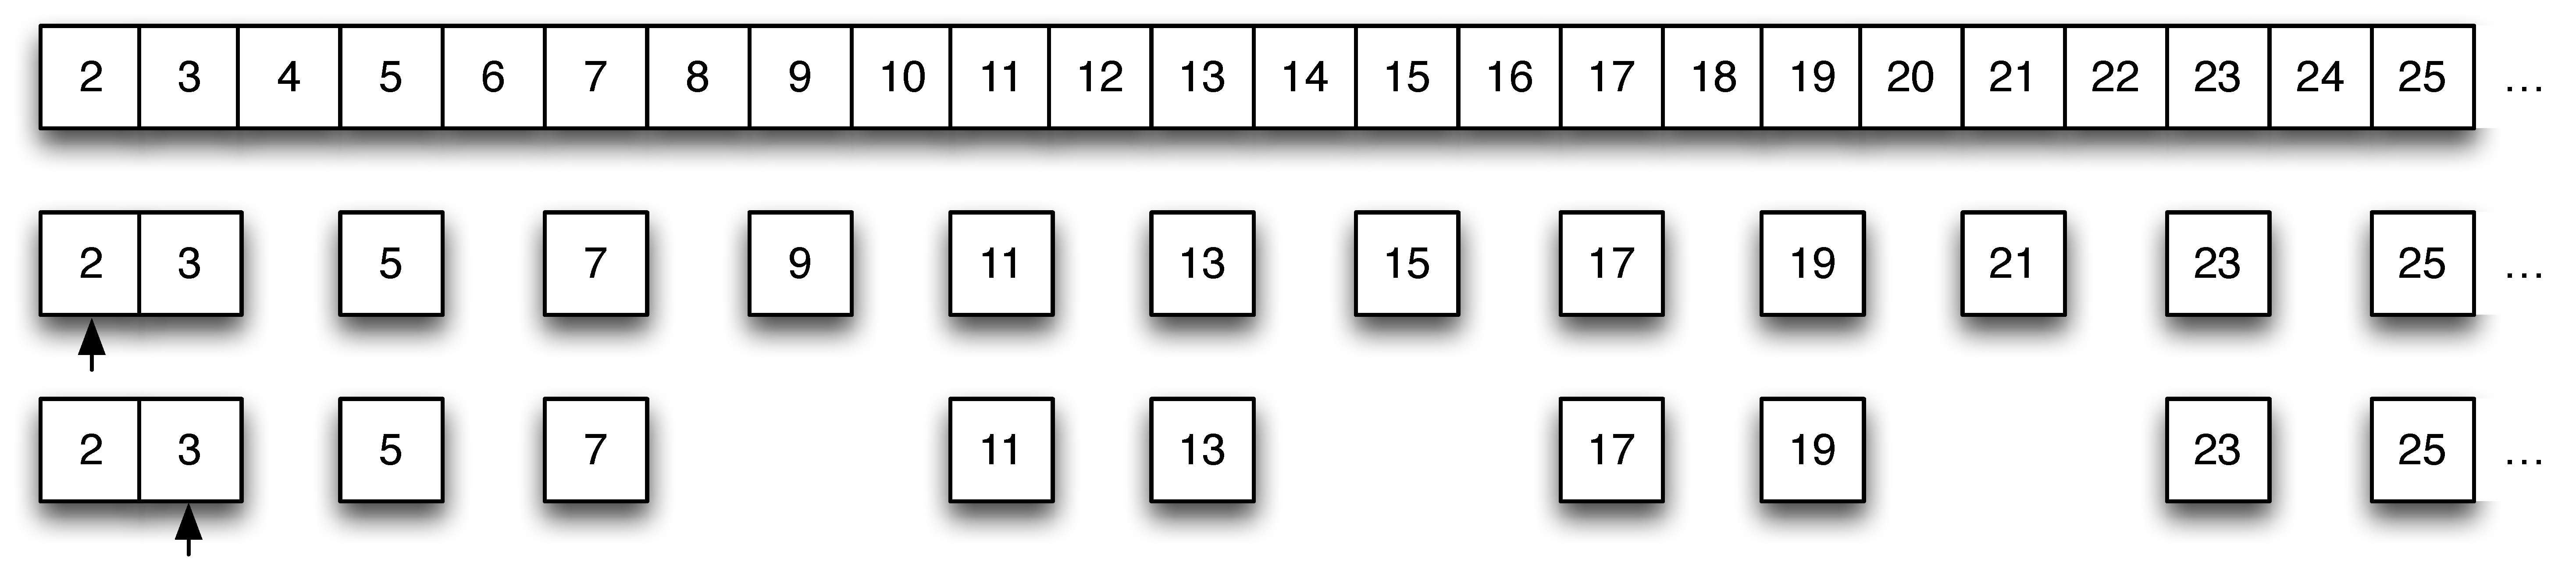
\includegraphics[width=5in]{Pictures/Sieve.pdf}
\end{center} 
\caption{The Sieve of Eratosthenes.}
\label{sievePic}
\end{figure}

We begin with the list of numbers starting at \texttt{2}. The head is
\texttt{2}, and we remove all the multiples of \texttt{2} from the list. The head
of the remainder of the list, \texttt{3}, is prime, since it was not removed in
the sieve by \texttt{2}. We therefore sieve the remainder of the list of
multiples of \texttt{3}, and repeat the process indefinitely. 
As a Haskell definition, we write
\begin{alltt}\minx{primes}\minx{sieve}
primes :: [Integer]

primes       = sieve [2 ..\ ]
sieve (x:xs) = x : sieve [ y | y <- xs , y `mod` x > 0]
\end{alltt}
where we test whether \texttt{x} divides 
\texttt{y} by evaluating \texttt{y `mod` x}; \texttt{y} is a multiple of \texttt{x} if this
value is zero. Beginning the evaluation, we have
\begin{alltt}
primes 
\step sieve [2 ..\ ]
\step 2 : sieve [ y | y <- [3 ..\ ] , y `mod` 2 > 0]
\step 2 : sieve (3 : [ y | y <- [4 ..\ ] , y `mod` 2 > 0])
\mbox{\texttt{\step 2 : 3 : sieve [ z | z <- [ y | y <- [4 ..\ ] , y `mod` 2 > 0],}}
                      z `mod` 3 > 0]  
\step ...
\step 2 : 3 : sieve [ z | z <- [5,7,9...] , z `mod` 3 > 0]  
\step ...
\step 2 : 3 : sieve [5,7,11,...]  
\step ...
\end{alltt}
Can we use \texttt{primes} to test for a number being a prime? If we evaluate 
\texttt{member primes 7} we get the response \texttt{True},
while \texttt{member primes 6} gives no answer. This is because an 
infinite number of elements have to be checked before we conclude that
\texttt{6} is not in the list. The problem is that \texttt{member} cannot use the
fact that \texttt{primes} is ordered. This we do in \texttt{memberOrd}.
\begin{alltt}\minx{memberOrd}
memberOrd :: Ord a => [a] -> a -> Bool
memberOrd (x:xs) n
  | x<n         = memberOrd xs n
  | x==n        = True
  | otherwise   = False
\end{alltt}
The difference here is in the final case: if the head of the list (\texttt{x)}
is greater
than the element we seek (\texttt{n}),
the element cannot be a member of the ordered list.
Evaluating the test again,
\begin{alltt}
memberOrd [2,3,5,7,11,...] 6
\step memberOrd [3,5,7,11,...] 6  
\step memberOrd [5,7,11,...] 6  
\step memberOrd [7,11,...] 6 
\step False
\end{alltt}
\vspace{5pt}

\subsubexample*{2. Generating random numbers}
\index{numbers!random}


Many computer systems require us to generate `random' numbers, one after
another. Our queuing simulation is a particular example upon which we focus
here, after looking at the basics of the problem.

No Haskell program can produce a truly random sequence; after all, we
want to be able to predict the behaviour of our programs, and randomness is
inherently unpredictable. What we can do, however, is generate a {\bf
pseudo-random}\index{pseudo-random numbers} sequence of natural numbers, smaller than \texttt{modulus}. 
This \textbf{linear congruential method} works by starting with a \texttt{seed},
and then by getting the next element of the sequence from the previous value
thus
\begin{alltt}
nextRand :: Integer -> Integer
nextRand n = (multiplier*n + increment) `mod` modulus
\end{alltt}
A (pseudo-)random sequence is given by iterating this function,
\begin{alltt}
randomSequence :: Integer -> [Integer]\minx{randomSequence}
randomSequence = iterate nextRand
\end{alltt}
Given the values
\begin{alltt}
seed       = 17489
multiplier = 25173
increment  = 13849
modulus    = 65536
\end{alltt}
the sequence produced by \texttt{randomSequence seed} begins
\begin{alltt}
[17489,59134,9327,52468,43805,8378,...
\end{alltt}
The numbers in this sequence, which range from \texttt{0} to \texttt{65535}, all
occur with the same frequency. What are we to do if instead we want the
numbers to come in the (integer) range \texttt{a} to \texttt{b} inclusive? We need
to scale the sequence, which is achieved by a \texttt{map}:
\begin{alltt}\minx{scaleSequence}
scaleSequence :: Integer -> Integer -> [Integer] -> [Integer]
scaleSequence s t
  = map scale
    where
    scale n = n `div` denom + s
    range   = t-s+1
    denom   = modulus `div` range
\end{alltt}
The original range of numbers \texttt{0} to \texttt{modulus-1} is split into 
\texttt{range} blocks, each of the same length. The number \texttt{s} is assigned to
values in the first block, \texttt{s+1} to values in the next, and so on.

In our simulation example, we want to generate for each arrival the length of 
service that person will need on being served. For illustration, we suppose
that they range from \texttt{1} to \texttt{6} minutes, but that they are supposed
to happen with different probabilities.
\begin{center}
\begin{tabular}{|l||c|c|c|c|c|c|}
\hline
Waiting time & \mi 1 & \mi 2 & \mi 3 & \mi 4 & \mi 5 & \mi 6 \\ \hline
Probability & \mi 0.2 & \mi 0.25 & \mi 0.25 & \mi 0.15 & \mi 0.1 & \mi 0.05 \\
\hline 
\end{tabular}
\end{center}
We need a function to turn such a distribution into a transformer of
infinite lists. Once we have a function transforming individual values, we
can \texttt{map} it along the list.

We can represent a distribution of objects of type \texttt{a} by a list of type
\texttt{[(a,Float)]}, where we assume that the numeric entries add up to one.  Our
function transforming individual values will be
\begin{alltt}
makeFunction :: [(a,Float)] -> (Float -> a)\minx{makeFunction}
\end{alltt}
so that numbers in the range \texttt{0} to \texttt{65535} are transformed into
items of type \texttt{a}. The idea of the function 
is to give the following ranges to the entries for the list above.
\begin{center}
\begin{tabular}{|l||c|c|c|c|}
\hline
Waiting time & \mi 1 & \mi 2 & \mi 3 & \mi \ldots  \\ \hline
Range start& \mi 0 & \mi (m*0.2)+1 & 
\mi (m*0.45)+1 & \mi \ldots  \\ \hline 
Range end& \mi m*0.2 & \mi m*0.45 & 
\mi m*0.7 & \mi \ldots  \\ \hline 
\end{tabular}
\end{center}
where \texttt{m} is used for \texttt{modulus}.
The definition follows:
\begin{alltt}
makeFunction dist = makeFun dist 0.0

makeFun ((ob,p):dist) nLast rand
  | nNext >= rand \&\& rand > nLast     
        = ob
  | otherwise                           
        = makeFun dist nNext rand
          where
          nNext = p*fromIntegral modulus + nLast
\end{alltt}
The \texttt{makeFun} function has an extra argument, which carries the position
in the range \texttt{0} to \texttt{modulus-1} reached so far in the search; it is
initially zero. The \texttt{fromIntegral} function used here converts an \texttt{Int} to
an equivalent \texttt{Float}.

The transformation of a list of random numbers is given by
\begin{alltt}
map (makeFunction dist)
\end{alltt}
and the random distribution of waiting times we require begins
thus
\begin{alltt}
map (makeFunction dist . fromIntegral) (randomSequence seed)
= [2,5,1,4,3,1,2,5,4,2,2,2,1,3,2,5,...
\end{alltt}
with \texttt{6} first appearing at the \texttt{35}th position.


A full library for generating random numbers and random data for other types is given in  
\texttt{System.Random}.\minx{System.Random}

\begin{figure}[t]
\beware{Infinite list generators}{\index{list comprehensions!infinite generators}%
\index{pitfalls!infinite list generators}%
The list comprehension \texttt{pythagTriples2}, intended to produce the list of
all Pythagorean triples, instead produces {\em no\/} output to the prompt. 
\index{Pythagorean triple}
\begin{alltt}
pythagTriples2 =
\end{alltt}
\vspace*{-17pt}
\begin{alltt}
\ \ =\ [ (x,y,z) | x <- [2 .. ] ,
\end{alltt}
\vspace*{-17pt}
\begin{alltt}
\ \ \ \ \ \ \ \ \ \ \ \ \ \ \ \ y <- [x+1 .. ] ,
\end{alltt}
\vspace*{-17pt}
\begin{alltt}
\ \ \ \ \ \ \ \ \ \ \ \ \ \ \ \ z <- [y+1 .. ] ,
\end{alltt}
\vspace*{-17pt}
\begin{alltt}
\ \ \ \ \ \ \ \ \ \ \ \ \ \ \ \ x*x + y*y == z*z ]
\end{alltt}
The
problem is in the order of choice of the elements. The first choice for 
\texttt{x} is \texttt{2}, and for \texttt{y} is \texttt{3}; given this, 
there are an infinite
number of values to try for \texttt{z}: \texttt{4}, \texttt{5} and so
on, indefinitely. We therefore never try any of the other choices for
\texttt{x} or \texttt{y}, among which the triples lie.

Two options present themselves. First we can redefine the solution, as
in the original
\texttt{pythagTriples}, so that it involves only one infinite list.
Alternatively, we can try to write a function which returns all pairs of 
elements from two infinite lists:
\begin{alltt}
infiniteProduct :: [a] -> [b] -> [(a,b)]
\end{alltt}
This is left as an exercise. Using such a function it is possible to adapt the
definition of \texttt{pythagTriples2} to make it give all the Pythagorean triples.
}
\end{figure}

\end{example}
\begin{exercises}

\item 
Define the infinite lists of factorial and Fibonacci numbers, 
\begin{alltt}
factorial = [1,1,2,6,24,120,720,...]
fibonacci = [0,1,1,2,3,5,8,13,21,...]
\end{alltt}

\item
Give a definition of the function
\begin{alltt}
factors :: Int -> [Int]
\end{alltt}
which returns a list containing the factors of a positive integer. For
instance,
\begin{alltt}
factors 12 = [1,2,3,4,6,12]
\end{alltt}
Using this function or otherwise, define the list of numbers whose only prime
factors are \texttt{2}, \texttt{3} and \texttt{5}, the so-called \textbf{Hamming numbers}:
\index{Hamming numbers}\label{HamNos}
\begin{alltt}
hamming = [1,2,3,4,5,6,8,9,10,12,15,...
\end{alltt}

\item
Define the function
\begin{alltt}
runningSums :: [Int] -> [Int]
\end{alltt}
which calculates the running sums
\begin{alltt}
[0,\subscr{a}{0},\subscr{a}{0}+\subscr{a}{1},\subscr{a}{0}+\subscr{a}{1}+\subscr{a}{2},...
\end{alltt}
of a list
\begin{alltt}
[\subscr{a}{0},\subscr{a}{1},\subscr{a}{2},...
\end{alltt}

\item
Define the function \texttt{infiniteProduct} specified above, and use it to
correct the definition of \texttt{pythagTriples2}.
\end{exercises}
\section{Why infinite lists?}
\label{whyInfLis}
\index{design!and infinite lists|(}
\index{lists!infinite!why?}
\index{infinite lists|see{lists, infinite}}

Haskell supports infinite lists and other infinite structures, 
and we saw in the last section that we could define a number of quite
complicated
lists, like the list of prime numbers, and lists of random numbers. The
question remains, though, of whether these lists are anything other than a
curiosity. There are two arguments which show their importance in functional
programming.

First, an infinite version of a program can be more \textbf{abstract}, and so simpler
\index{abstraction}
to write. Consider the problem of finding the \texttt{n}th prime number, using the
Sieve of Eratosthenes. If we work with finite lists, we need to know in
advance how large a list is needed to accommodate the first \texttt{n} primes; if
we work with an infinite list, this is not necessary: only that part of the
list which is needed will be generated as computation proceeds.\looseness=1

In a similar way, the random numbers given by \texttt{randomSequence seed}
provided an unlimited resource: we can take as many random numbers from the
list as we require. There needs to be no decision at the start of programming
as to the size of sequence needed. (These arguments are rather like those for
\textbf{virtual memory} in a computer. It is often the case that predicting
the memory use of a program is possible, but tiresome; virtual memory makes
this unnecessary, and so frees the programmer to proceed with other tasks.)

The second argument is of wider significance, and can be seen by re-examining
the way in which we generated random numbers. We generated an infinite list
by means of \texttt{iterate}, and we transformed the values using \texttt{map};
these operations are pictured in Figure \ref{processes1}
as a generator of and a transformer of lists of values. These
values are shown in the dashed boxes.\index{lists!as
processes}\index{processes}
These components can then be linked together, giving more complex
combinations, as in Figure \ref{processes2}.
\begin{figure}[t]
\begin{center}
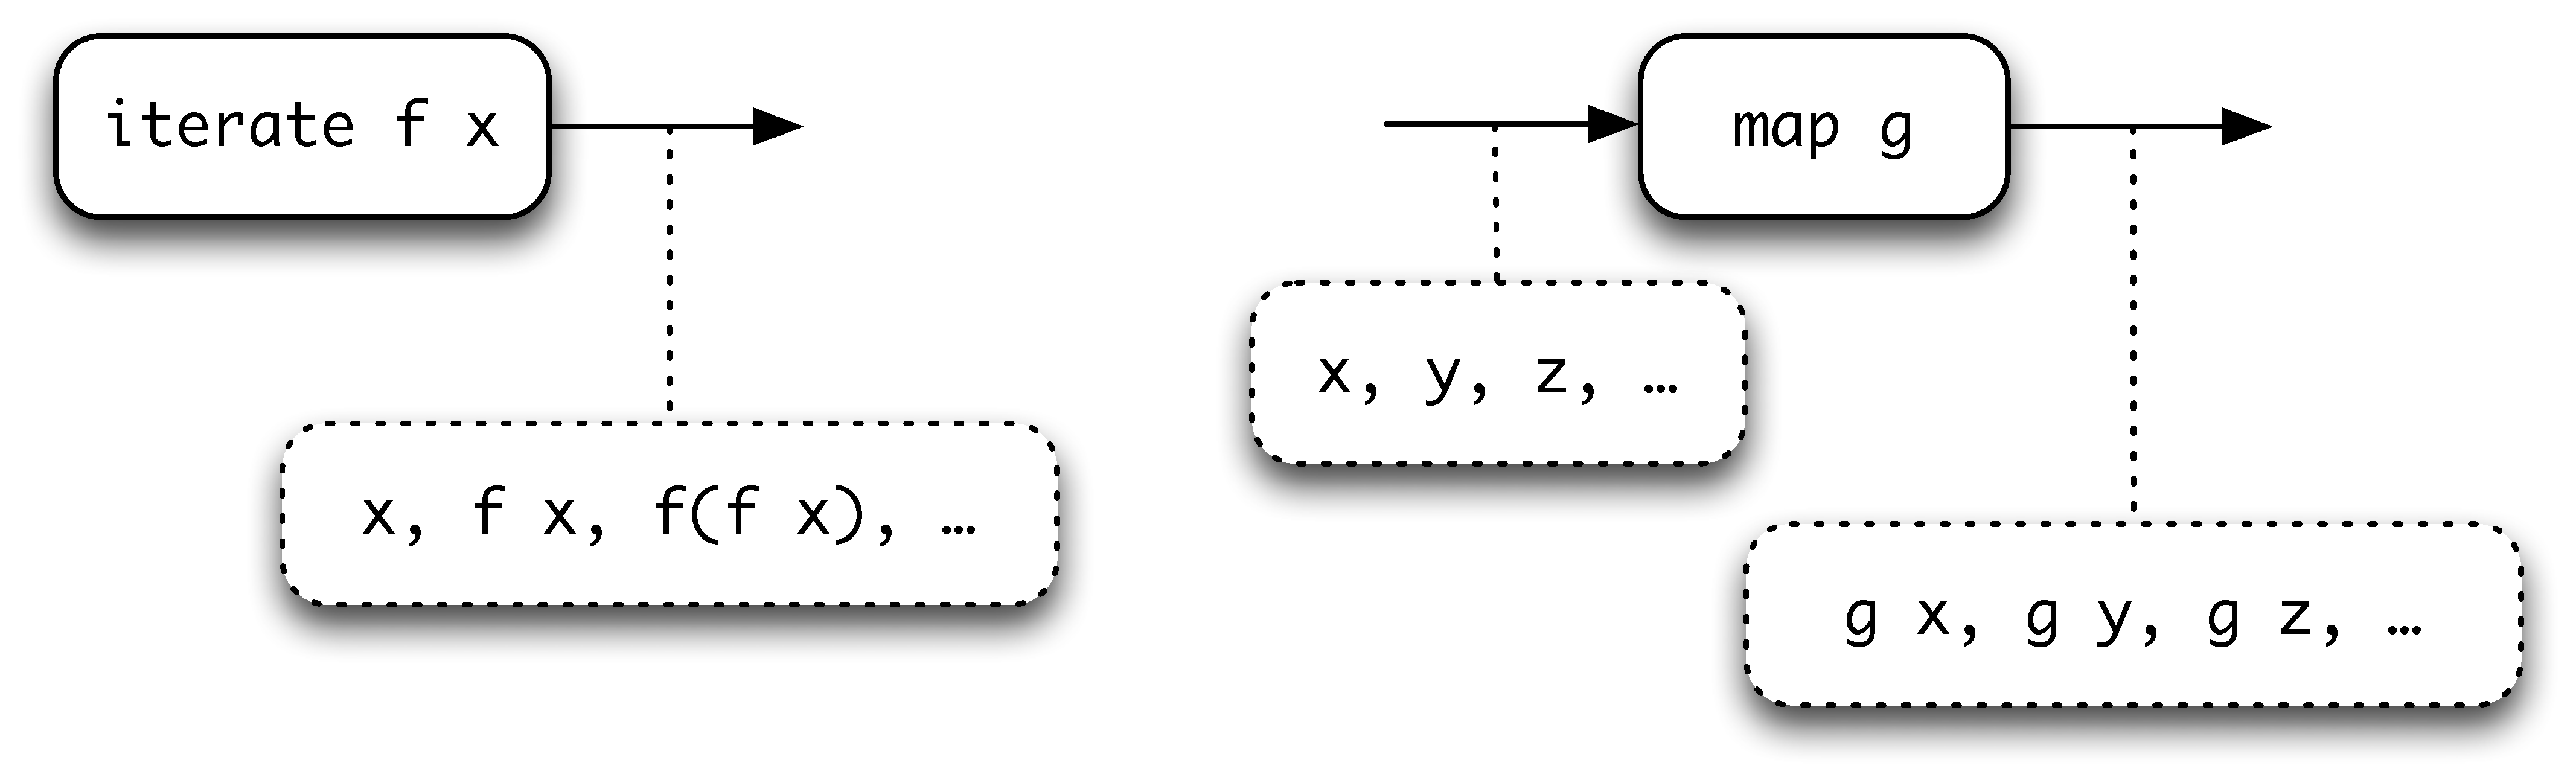
\includegraphics[width=5in]{Pictures/Processes1.pdf}
\end{center} 
\caption{A generator and a transformer.}
\label{processes1}
\end{figure}
\begin{figure}[t]
\begin{center}
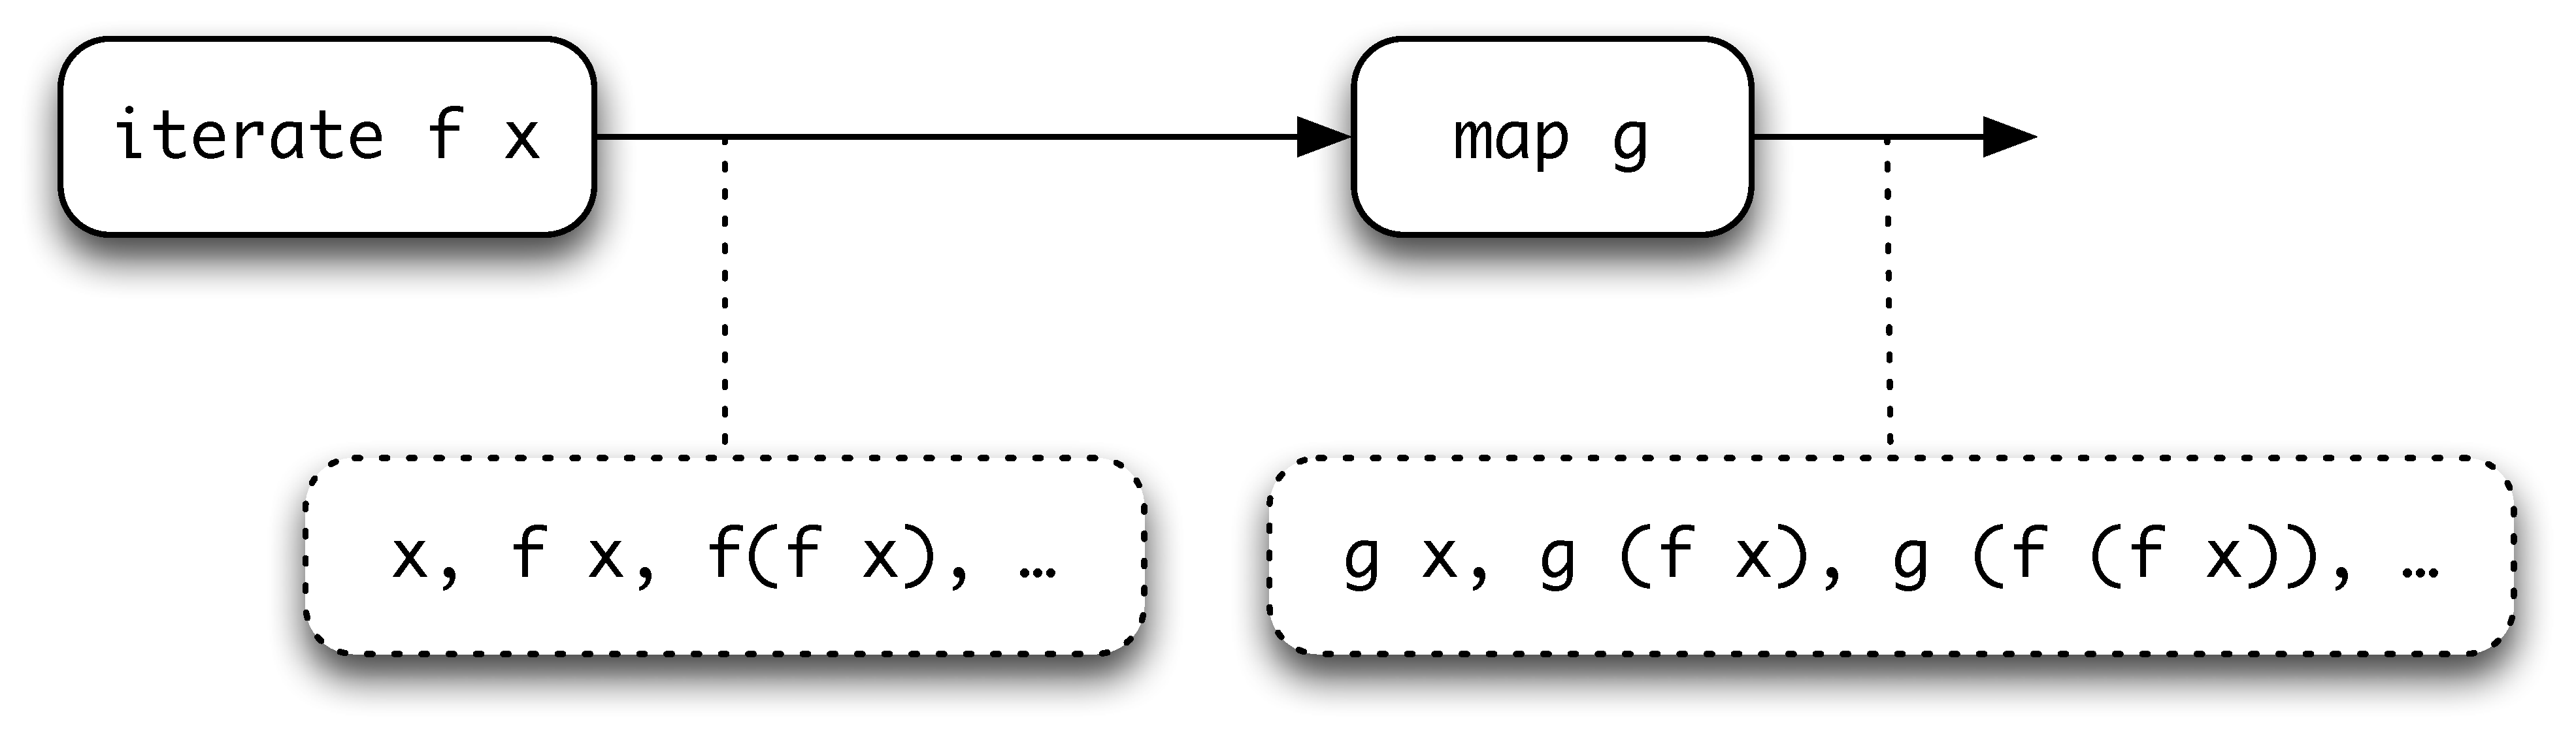
\includegraphics[width=5in]{Pictures/Processes2.pdf}
\end{center} 
\caption{Linking processes together.}
\label{processes2}
\end{figure}
This approach \textbf{modularizes} the generation of values in a distribution in
an interesting way. We have separated the generation of the values from
their transformation, and this means we can change each part independently of
the other.

Once we have seen the view of infinite lists as the links between
processes, other combinations suggest themselves, and in particular we can
begin to write process-style programs which involve \textbf{recursion}.
\index{recursion}

Among the exercises in the last section was the problem of finding the running
sums
\begin{alltt}
[0,\subscr{a}{0},\subscr{a}{0}+\subscr{a}{1},\subscr{a}{0}+\subscr{a}{1}+\subscr{a}{2},...
\end{alltt}
of the list \texttt{[\subscr{a}{0},\subscr{a}{1},\subscr{a}{2},...}. Given the
sum up to \texttt{\subscr{a}{k}}, say, we get the next sum by adding the next
value in the input, \texttt{\subscr{a}{k+1}}. It is as if we {\em feed the sum
back\/}\index{feedback}
into the process to have the value \texttt{\subscr{a}{k+1}} added. This
is precisely the effect of the network of processes in Figure \ref{sumStream}, where
the values passing along the links are shown in the dotted boxes.\looseness=1
\begin{figure}
\begin{center}
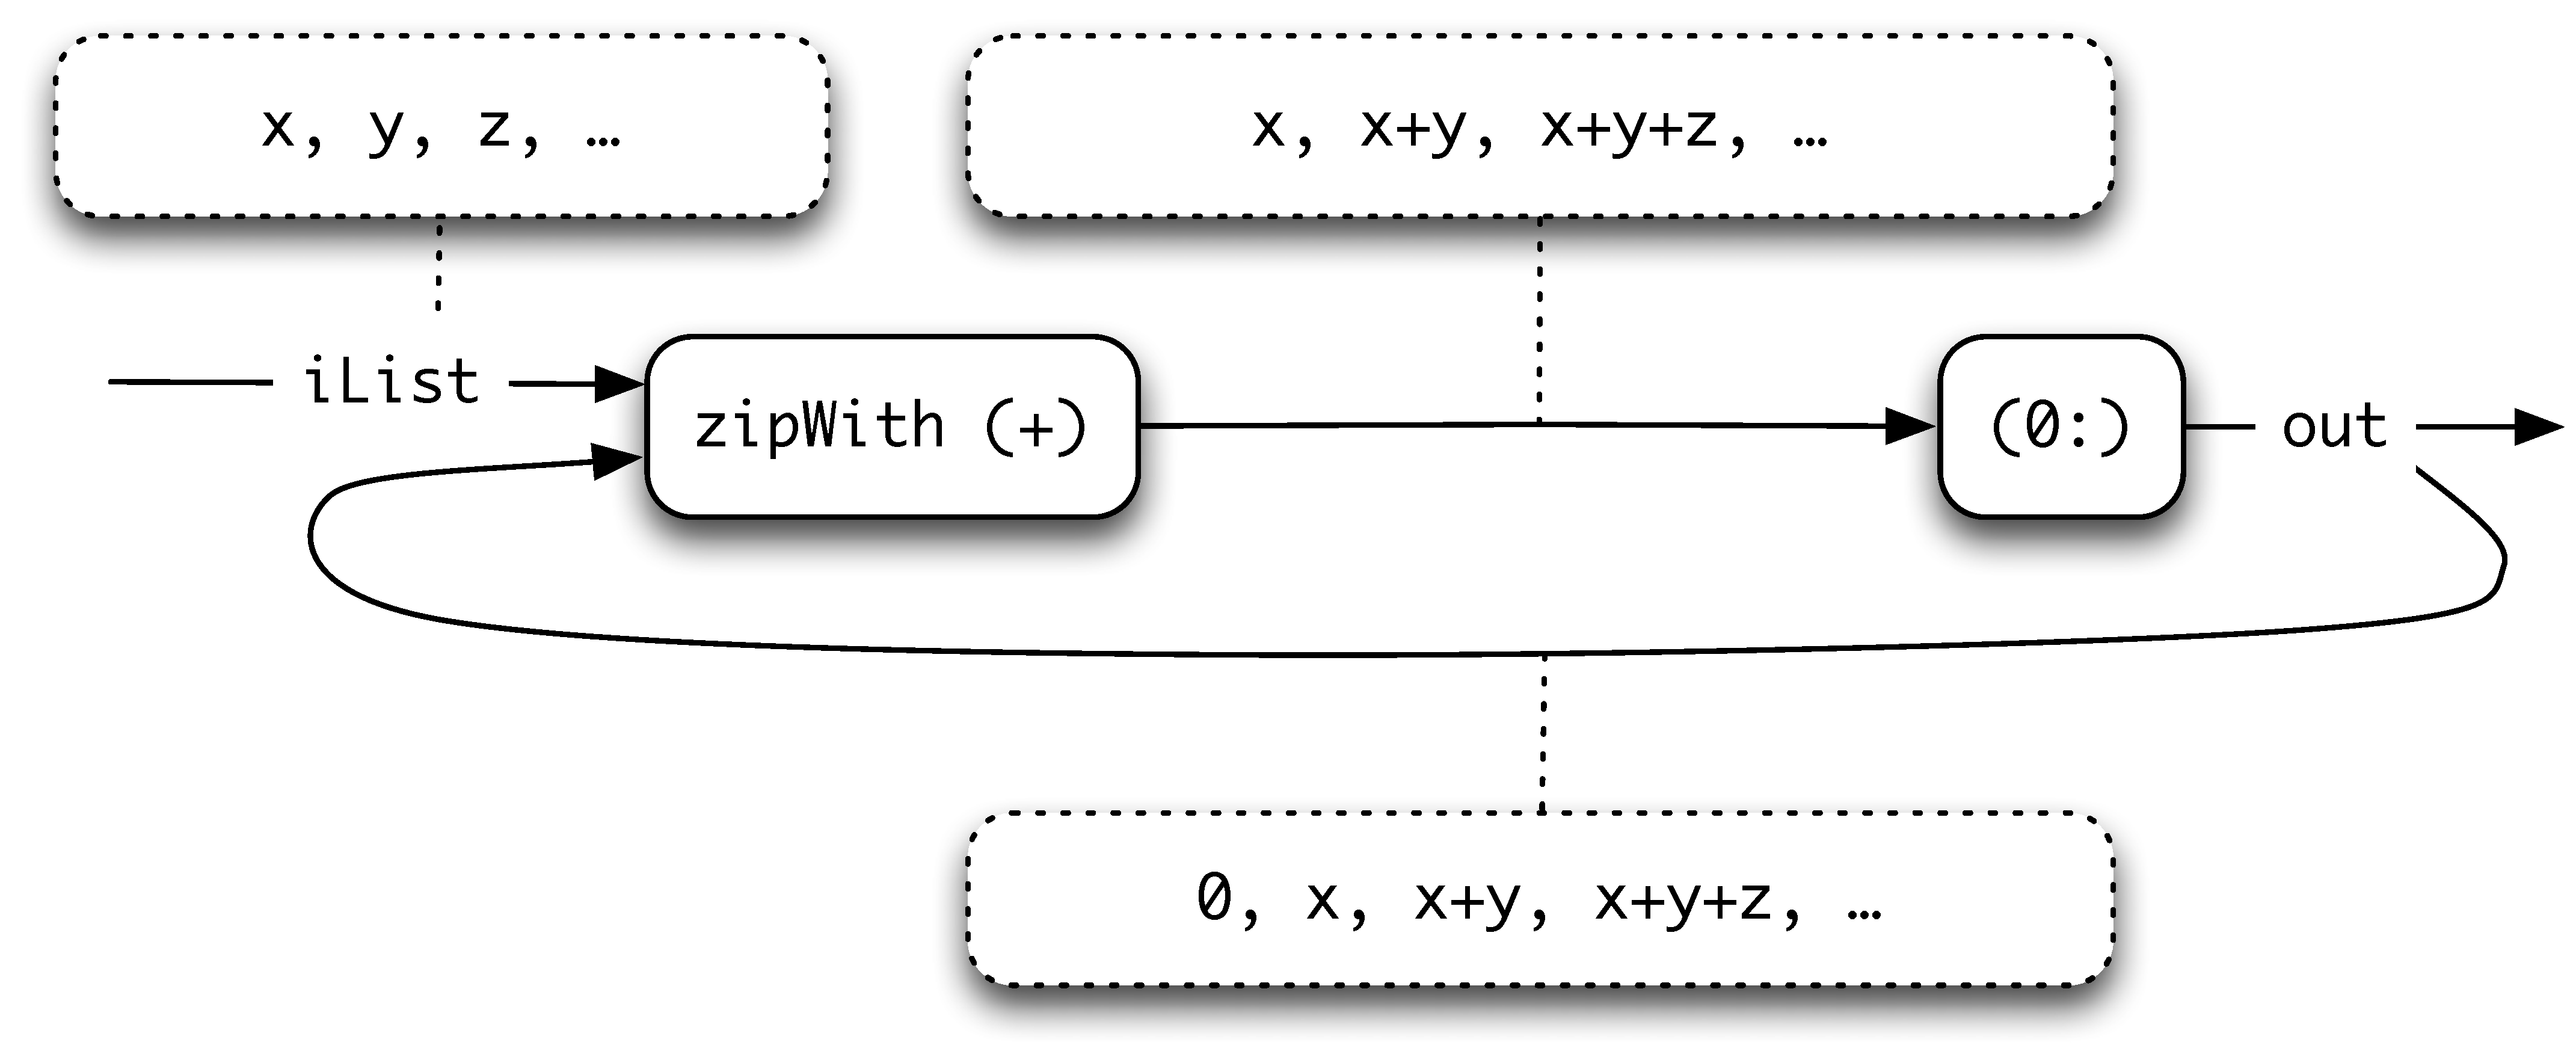
\includegraphics[width=5in]{Pictures/Processes3.pdf}
\end{center}
\caption{A process to compute the running sums of a list.}
\label{sumStream}
\end{figure}

The first value in the output \texttt{out} is \texttt{0}, and we get  the remaining values 
 by adding the next value in \texttt{iList} to the previous sum, appearing in
the list \texttt{out}.
This is translated into Haskell as follows. The output of the function on 
input \texttt{iList} is \texttt{out}. This is itself got by adding \texttt{0} to the
front of the output from the \texttt{zipWith (+)}, which itself has inputs 
\texttt{iList} and \texttt{out}. In other words,
\begin{alltt} 
listSums :: [Integer] -> [Integer]

listSums iList = out
                 where
                 out = 0 : zipWith (+) iList out
\end{alltt} 
where we recall that \texttt{zipWith} is defined by\index{zipWith@\texttt{zipWith}}
\begin{alltt}
zipWith f (x:xs) (y:ys) = f x y : zipWith f xs ys
zipWith f _     _       = []
\end{alltt}
and the operator section \texttt{(0:)} puts a zero on the front of a list. 
We give a calculation of an example now.
\begin{alltt}\minx{listSums}
listSums [1 ..\ ]
\step out
\step 0 : zipWith (+) [1 ..\ ] out
\step 0 : zipWith (+) [1 ..\ ] (0:...) \hfill(1)
\step 0 : 1+0 : zipWith (+) [2 ..\ ] (1+0:...)\hfill(2)
\step 0 : 1 : 2+1 : zipWith (+) [3 ..\ ] (2+1:...)  \step ...
\end{alltt} 
In making this calculation, we replace the occurrence of \texttt{out} in line
\texttt{(1)} with the incomplete list \texttt{(0:...)}. In a similar way, we
replace the tail of \texttt{out} by \texttt{(1+0:...)} in line \texttt{(2)}.

The definition of \texttt{listSums} is an example of the general function \texttt{scanl'},
which combines values using the function \texttt{f}, and whose first output is
\texttt{st}.
\begin{alltt}
scanl' :: (a -> b -> b) -> b -> [a] -> [b]\index{scanl@\texttt{scanl\symbol{39}}}
scanl' f st iList
  = out 
    where
    out = st : zipWith f iList out
\end{alltt}
The function \texttt{listSums} is given by \texttt{scanl' (+) 0}, and a function which
keeps a running sort of the initial parts of list is 
\texttt{sorts = scanl' ins []}, where \texttt{ins} inserts an element in the
appropriate place in a sorted list. The list of factorial values, 
\texttt{\index{factorial}
[1,1,2,6,...]} is given by \texttt{scanl' (*) 1 [1 ..\ ]}, and taking this as a
model, any primitive recursive function \index{primitive recursion}
can be described in a similar way.

The definition we give here is a minor variant of
the standard function \texttt{scanl},\minx{scanl}
but we choose to give the definition here because of its close
correspondence to the process networks for running sums given in Figure
\ref{sumStream}.

\begin{exercises}

\item
Give a definition of the list \texttt{[ 2\^{}n | n <- [0 ..\ ] ]} using a process
network based on \texttt{scanl'}. (Hint: you can take the example of factorial as a
guide.)

\item
How would you select certain elements of an infinite list? For instance, how
would you keep running sums of the {\em positive\/} numbers in a list of
numbers?

\item
How would you {\em merge\/} two infinite lists, assuming that they are
sorted?
How would you remove duplicates from the list which results? As an example,
how would you merge the lists of powers of \texttt{2} and \texttt{3}?

\item
Give definitions of the lists of Fibonacci numbers 
\texttt{\index{Fibonacci numbers}
[0,1,1,2,3,5,...]} and Hamming numbers \texttt{[1,2,3,4,5,6,8,9,...]} (defined on
page \pageref{HamNos}) using 
\index{Hamming numbers}
networks of processes. For the latter problem, you may find
the merge function of the previous question useful.

\index{design!and infinite lists|)}

\end{exercises}

\section{Case study: simulation}
\index{simulation|(}

We are now in a position to put together the ingredients of the queue
simulation covered in 
\begin{titemize}
\item Section \ref{algDesign}, where we designed the algebraic types
\texttt{Inmess} and \texttt{Outmess},
\item Section \ref{simEx}, where the abstract types \texttt{QueueState} and 
\texttt{ServerState} were introduced, and in 
\item Section \ref{infLists}, where we showed how to generate an infinite list
of pseudo-random waiting times chosen according to 
a distribution over the times \texttt{1} to \texttt{6}.
\end{titemize}
As we said in Section \ref{algDesign}, our top-level simulation will be a
function from a series of input messages to a series of output messages, so
\begin{alltt}
doSimulation :: ServerState -> [Inmess] -> [Outmess]
\end{alltt}
where the first parameter is the state of the server at the start of the
simulation. In Section \ref{simEx} we presented the function performing
one step of the simulation,
\begin{alltt}
simulationStep :: ServerState -> 
                  Inmess -> 
                  (ServerState, [Outmess])
\end{alltt}
which takes the current server state, and the input message arriving at the
current minute and returns the state after one minute's  processing, paired
with the list of the output messages produced by the queues that minute (potentially
every queue could release a customer at the same instant, just as no
customers might be released.)

The output of the simulation will be given by the output messages generated
in the first minute, and after those the results of a new simulation beginning
with the updated state:
\begin{alltt}
doSimulation servSt (im:messes)
  = outmesses ++ doSimulation servStNext messes
    where
    (servStNext , outmesses) = simulationStep servSt im
\end{alltt}
How do we generate an input sequence? From Section \ref{infLists} we have the 
sequence of times given by 
\begin{alltt}
randomTimes \minx{randomTimes}
  = map (makeFunction dist . fromIntegral) (randomSequence seed)
  \step [2,5,1,4,3,1,2,5,...
\end{alltt}
We are to have arrivals of one person per minute, so the input messages we
generate are
\begin{alltt}
simulationInput 
  = zipWith Yes [1 ..\ ] randomTimes \minx{simulationInput}
  \step [ Yes 1 2 , Yes 2 5 , Yes 3 1 , Yes 4 4 , Yes 5 3 ,...
\end{alltt}
What are the outputs produced when we run the simulation on this input with
four queues, by setting the constant \texttt{numQueues} to \texttt{4}? The output
begins
\begin{alltt}
doSimulation serverStart simulationInput
\step [Discharge 1 0 2, Discharge 3 0 1, Discharge 6 0 1, 
     Discharge 2 0 5, Discharge 5 0 3, Discharge 4 0 4,
     Discharge 7 2 2,...
\end{alltt}
The first six inputs are processed without delay, but the seventh requires a
waiting time of \texttt{2} before being served. 

The infinite number of arrivals
represented by \texttt{simulationInput} will obviously generate a corresponding
infinite number of output messages. We can make a finite approximation by
giving the input
\begin{alltt}
simulationInput2 = take 50 simulationInput ++ noes
noes = No : noes
\end{alltt}
where after one arrival in each of the first 50 minutes, no further
people arrive. Fifty output messages will be generated, and we define this
list of outputs thus:
\begin{alltt}
take 50 (doSimulation serverStart simulationInput2)
\end{alltt}

\subsection*{Experimenting}
\index{simulation!experimenting}

We now have the facilities to begin experimenting with different data, such
as the distribution and the number of queues. The total waiting time for a
(finite) sequence of \texttt{Outmess} is given by
\begin{alltt}
totalWait :: [Outmess] -> Int
totalWait = sum . map waitTime
            where
            waitTime (Discharge _ w _) = w
\end{alltt}
For \texttt{simulationInput2} the total waiting time is \texttt{29}, going up to
\texttt{287} with three queues and down to zero with five. We leave it to the
reader to experiment with the \textbf{round robin} simulation outlined in the
exercises of Section \ref{simEx}.

A more substantial project is to model a set-up with a single queue feeding a
number of bank clerks -- one way to do this is to extend the 
\texttt{serverState} with an extra queue which feeds into the individual queues: an
element leaves the feeder queue when one of the small queues is empty. This
should avoid the unnecessary waiting time we face when making the wrong
choice of queue, and the simulation shows that waiting times are reduced by
this strategy, though by less than we might expect if service times are short.

\index{simulation|)}
\index{lists!infinite|)}



\section{Proof revisited}
\label{lazyProof}

After summarizing the effect that lazy evaluation has on the types of
Haskell, we examine the consequences for reasoning about programs. Taking lists
as a representative example, we look at how we can prove properties of infinite
lists, and of all lists, rather than simply the set of finite
lists, which was the scope of the proofs we looked at in Chapters
\ref{reasoningProgs}, \ref{gen2} and \ref{algTypes}.

This section cannot give complete coverage of the issues of verification; we
conclude with pointers to further reading.

\subsection*{Undefinedness}
\index{undefinedness}

In nearly every programming language, it is possible to write a program which
fails to terminate, and Haskell is no exception. We call the value of such
programs the \textbf{undefined} value, as it gives no result to a computation.

The simplest expression which gives an undefined result is 
\begin{alltt}
undef :: a\minx{undef}
undef = undef\hfill(undef.1)
\end{alltt}
which gives a non-terminating or
undefined value of every type, but of course we can write an
undefined program without intending to, as in
\begin{alltt}
fak n = (n+1) * fak n
\end{alltt}
where we have confused the use of \texttt{n} and \texttt{n+1} in
attempting to define the
factorial function. The value of \texttt{fak n} will be the same as \texttt{undef}, as they
are both non-terminating.

We should remark that we
are using the term `undefined' in two different ways here. The \textbf{name}
\index{name}
\index{value!undefined}
\texttt{undef} is given a definition by \texttt{(undef.1)}; the \textbf{value} that the
definition gives it is the undefined value, which represents the result of a
calculation or evaluation which fails to terminate (and therefore fails to
define a result).

The existence of these undefined values has an effect on the type of lists.
What if we define, for example, the list
\begin{alltt}
list1 = 2:3:undef
\end{alltt}
The list has a well-defined head, \texttt{2}, and tail \texttt{3:undef}. Similarly,
the tail has a head, \texttt{3}, but its tail is undefined. The type \texttt{[Integer]}
therefore contains \textbf{partial} lists \index{lists!partial}
like \texttt{list1}, built from the
undefined list, \texttt{undef}, parts of which are defined and parts of which are
not.

Of course, there are also undefined
integers, so we also include in \texttt{[Integer]} lists like
\begin{alltt}
list2 = undef:[2,3]
list3 = undef:4:undef
\end{alltt}
which contain undefined values, and might also be partial. Note that in 
\texttt{list3} the first occurrence of \texttt{undef} is at type \texttt{Integer} while the
second is at type \texttt{[Integer]}.

What happens when a function is applied to \texttt{undef}? We use the rules for
calculation we have seen already, so that the \texttt{const} function of the 
standard prelude satisfies
\begin{alltt}
const 17 undef \step 17
\end{alltt}
If the function applied to \texttt{undef} has to pattern match, then the result of
the function will be \texttt{undef}, since the pattern match has to look at the
structure of \texttt{undef}, which will never terminate. For instance, for the
functions used in Chapter \ref{reasoningProgs},
\begin{alltt}
sum undef       \step undef \hfill (sum.u)
doubleAll undef \step undef \hfill (doubleAll.u)
\end{alltt}
In writing proofs earlier in the book we were careful to state that in some
cases the results hold only for \textbf{defined} values. \index{value!defined}

An integer is defined \index{numbers!defined}
if it is not equal to \texttt{undef}; a list is defined \index{lists!defined}
if it
is a finite list of defined values; using this as a model it is not
difficult to give a definition of the defined values of any algebraic type. 
 
A
finite list as we have defined it may contain undefined values. Note that in
some earlier proofs we stipulated that the results hold only for (finite)
lists of defined values, that is for defined lists.



\subsection*{List induction revisited}

As we said above, since there is an undefined list, \texttt{undef}, in each list
type, lists can be built up from this; there will therefore be two base
cases in the induction principle.

\subsubsection*{Proof by structural induction: fp-lists} 
\index{structural induction}

To prove the property \texttt{P(xs)} for all finite or partial lists
(\textbf{fp-lists}) \texttt{xs} we have to do three things:
\index{fp-list}
\index{lists!finite/partial}

\medskip
\noindent
\begin{mytable}
\bf Base cases & Prove \texttt{P([])} and \texttt{P(undef)}. \\
\bf Induction step & Prove \texttt{P(x:xs)} assuming that \texttt{P(xs)} holds
already.
\end{mytable}

\medskip
\noindent
Among the results we proved by structural induction in Chapter \ref{reasoningProgs}
were the equations
\begin{alltt}
sum (doubleAll xs) = 2 * sum xs \hfill (sum-double)\minx{sum}\minx{doubleAll}
xs ++ (ys ++ zs)   = (xs ++ ys) ++ zs\hfill (assoc++)\minx{++}
reverse (xs ++ ys) = reverse ys ++ reverse xs\hfill (reverse++)\minx{reverse}
\end{alltt}
for all \textbf{finite} lists \texttt{xs}, \texttt{ys} and \texttt{zs}. For these results to
hold for all fp-lists, we need to show that
\begin{alltt}
sum (doubleAll undef) = 2 * sum undef \hfill (sum-double.u)
undef ++ (ys ++ zs)   = (undef ++ ys) ++ zs\hfill (assoc++.u)
reverse (undef ++ ys) = reverse ys ++ reverse undef\hfill (reverse++.u)
\end{alltt}
as well as being sure that the induction step is valid for all fp-lists.
Now, by \texttt{(sum.u)} and \texttt{(doubleAll.u)} the equation \texttt{(sum-double.u)} 
holds, and so \texttt{(sum-double)}
holds for all fp-lists. In a similar way, we can show \texttt{(assoc++.u)}.
More interesting is \texttt{(reverse++.u)}. Recall the definition of \texttt{reverse}:
\begin{alltt}
reverse []    = []
reverse (x:xs) = reverse xs ++ [x] 
\end{alltt}
It is clear from this that since there is a pattern match on the
parameter, \texttt{undef} as the first parameter will give an \texttt{undef}
result, so
\begin{alltt}
reverse undef = undef
\end{alltt}
Taking a defined list, like \texttt{[2,3]} for \texttt{ys} in \texttt{(reverse++.u)}
gives
\begin{alltt}
reverse (undef ++ [2,3])
  = reverse undef
  = undef

reverse [2,3] ++ reverse undef
  = [3,2] ++ undef
\end{alltt}
This is enough to show that \texttt{(reverse++.u)} does not hold, and that we cannot
infer that \texttt{(reverse++)} holds for all fp-lists. Indeed the example above shows
exactly that \texttt{(reverse++)} is not valid.

\subsection*{Infinite lists}
\index{lists!infinite}

Beside the fp-lists, there are \textbf{infinite} members of the list types.
How can we prove properties of infinite lists? A hint is given by our
discussion of printing the results of evaluating an infinite list. In practice
what happens is that we interrupt evaluation by hitting \texttt{Ctrl-C}
after some period of time. We can think of what we see on the screen as an
\textbf{approximation}\index{lists!infinite!approximation to} to the infinite list. 

If what we see are the elements 
\texttt{\subscr{a}{0},\subscr{a}{1},\subscr{a}{2},\ldots,\subscr{a}{n}}, we can think
of the approximation being the list
\begin{alltt}
\subscr{a}{0}:\subscr{a}{1}:\subscr{a}{2}:\ldots:\subscr{a}{n}:undef
\end{alltt}
since we have no information about the list beyond the element 
\texttt{\subscr{a}{n}}.

More formally, we say that the partial lists
\begin{alltt}
undef, \subscr{a}{0}:undef, \subscr{a}{0}:\subscr{a}{1}:undef, \subscr{a}{0}:\subscr{a}{1}:\subscr{a}{2}:undef, \ldots
\end{alltt}
are approximations to the infinite list 
\texttt{[\subscr{a}{0},\subscr{a}{1},\subscr{a}{2},\ldots,\subscr{a}{n},\ldots]}. 

Two lists \texttt{xs} and \texttt{ys} are equal if all their
approximants are equal, that is for all natural numbers \texttt{n},
\texttt{take n xs = take n ys}.
(The \texttt{take} function gives the defined portion of the \texttt{n}th
approximant, and it is enough to compare these parts.) A more usable
version of this principle applies to infinite lists only.

\subsubsection*{Infinite list equality}
\index{equality!infinite lists}
A list \texttt{xs} is infinite if for all natural numbers
\texttt{n}, \texttt{take n xs
\noteq\ take (n+1) xs}.\\
Two infinite lists \texttt{xs} and \texttt{ys} are equal if for all natural
numbers \texttt{n},
\texttt{xs!!n = ys!!n}.

\subsection*{Example}
\subsubsection*{Two factorial lists}

Our example here is inspired by the process-based programs of Section
\ref{whyInfLis}. If \texttt{fac} is the factorial function
\begin{alltt}
fac :: Int -> Int\minx{fac}
fac 0 = 1\hfill (fac.1)
fac m = m * fac (m-1)\hfill (fac.2)
\end{alltt}
one way of defining the infinite list of factorials is
\begin{alltt}\minx{facMap}
facMap = map fac [0 ..\ ]\hfill (facMap.1) 
\end{alltt}
while a process-based solution is
\begin{alltt}\minx{facs}
facs = 1 : zipWith (*) [1 ..\ ] facs\hfill (facs.1)
\end{alltt}
Assuming these lists are infinite (which they clearly are), we have to prove
for all natural numbers \texttt{n} that 
\begin{alltt}
facMap!!n = facs!!n \hfill (facMap.!!)
\end{alltt}
\startpr
In our proof we will assume for all natural numbers \texttt{n} the results
\begin{alltt}
(map f xs)!!n        = f (xs!!n)\hfill (map.!!)
(zipWith g xs ys)!!n = g (xs!!n) (ys!!n)\hfill (zipWith.!!)
\end{alltt}
which we discuss again later in this section.
 
\texttt{(facMap.!!)} is proved by mathematical induction\index{mathematical induction},
that is we prove the result for \texttt{0} outright, and we prove the
result for a positive \texttt{n} assuming the result for \texttt{n-1}.

\subparagraph*{Base}
We start by proving the
result at zero. Examining the left-hand side first,
\begin{alltt}
facMap!!0 
  = (map fac [0 ..\ ])!!0 \hfill {\rm by} (facMap.1)
  = fac ([0 ..\ ]!!0) \hfill {\rm by} (map.!!)
  = fac 0\hfill {\rm by def of} [0 ..\ ],!!
  = 1 \hfill {\rm by} (fac.1)
\end{alltt}
The right-hand side is
\begin{alltt}
facs!!0
  = (1 : zipWith (*) [1 ..\ ] facs)!!0 \hfill {\rm by} (facs.1)
  = 1\hfill {\rm by def of} !!
\end{alltt}
thus establishing the base case. 

\subparagraph*{Induction}
In the induction case we have to prove \texttt{(facMap.!!)}
using the induction hypothesis:
\begin{alltt}
facMap!!(n-1) = facs!!(n-1) \hfill (hyp)
\end{alltt}
The left-hand side of \texttt{(facMap.!!)} is
\begin{alltt}
facMap!!n
  = (map fac [0 ..\ ])!!n \hfill {\rm by} (facMap.1)
  = fac ([0 ..\ ]!!n) \hfill {\rm by} (map.!!)
  = fac n \hfill {\rm by def of} [0 ..\ ],!!
  = n * fac (n-1) \hfill {\rm by} (fac.2)
\end{alltt}
It is not hard to see that we have 
\texttt{facMap !!\ (n-1) = fac (n-1)} by a similar argument to the first three steps here
and so,
\begin{alltt}
  = n * (facMap!!(n-1))
\end{alltt}
The right-hand side of \texttt{(facMap.!!)} is 
\begin{alltt}
facs!!n
  = (1 : zipWith (*) [1 ..\ ] facs)!!n \hfill{\rm by} (facs.1)
  = (zipWith (*) [1 ..\ ] facs)!!(n-1) \hfill {\rm by def of} !!
  = (*) ([1 ..\ ]!!(n-1)) (facs!!(n-1))\hfill {\rm by} (zipWith.!!)
  = ([1 ..\ ]!!(n-1)) * (facs!!(n-1))\hfill {\rm by def of} (*)
  = n * (facs!!(n-1)) \hfill {\rm by def of} [1 ..\ ],!!
  = n * (facMap!!(n-1)) \hfill {\rm by} (hyp)
\end{alltt}
The final step of this proof is given by the induction hypothesis, and
completes the proof of the induction step and the result itself. \blackbox

\subsection*{Proofs for infinite lists}

When are results we prove for all fp-lists valid for all lists? If a
result holds for all fp-lists, then it holds for all {\em approximations\/}
to infinite lists. For some properties it is enough to know the property
for all approximations to know that it will be valid for all infinite lists
as well. In particular, this is true for all {\em equations\/}. This means
that, for example, we can assert that for {\em all\/} lists \texttt{xs},
\begin{alltt}
(map f . map g) xs = map (f.g) xs
\end{alltt}
and therefore by the principle of extensionality for functions,
\index{extensionality principle}
\begin{alltt}
map f . map g = map (f.g)
\end{alltt}
Many other of the equations we proved initially for finite lists can be
extended to proof for the fp-lists, and therefore to all lists. Some
of these are given in the exercises which follow.

\subsection*{Further reading}

The techniques we have given here provide a flavour of how to write
proofs for
infinite lists and infinite data structures in general. We cannot give the
breadth or depth of a full presentation, but refer the reader to 
\citeN{logicandcomp} for
more details. An alternative approach to proving the factorial list
example is given in \citeN{sjtProofFP}, which also gives a survey of proof
in functional programming.



\begin{exercises}

\item
Show that for all fp-lists \texttt{ys} and \texttt{zs},
\begin{alltt}
undef ++ (ys ++ zs)  = (undef ++ ys) ++ zs
\end{alltt}
to infer that \texttt{++} is associative over all lists.

\item
If \texttt{rev xs} is defined to be \texttt{shunt xs []}, as
in Section \ref{genPrf}, show that
\begin{alltt}
rev (rev undef) = undef \hfill (rev-rev.1)
\end{alltt}
In Chapter \ref{reasoningProgs} we proved that 
\begin{alltt}
rev (rev xs) = xs \hfill (rev-rev.2)
\end{alltt}
for all
finite lists \texttt{xs}. 

Why can we not infer from \texttt{(rev-rev.1)} and \texttt{(rev-rev.2)}
that the equation \texttt{rev (rev xs) = xs} holds for all fp-lists \texttt{xs}? 

\item
Prove for all natural numbers \texttt{m}, \texttt{n} and functions 
\texttt{f ::\ Int -> a} that 
\begin{alltt}
(map f [m ..\ ])!!n = f (m+n)
\end{alltt}
[Hint: you will need to choose the right variable for the induction proof.]

\item
Prove that the lists
\begin{alltt}
facMap = map fac [0 ..\ ]
facs = 1 : zipWith (*) [1 ..\ ] facs
\end{alltt}
are infinite.

\item
If we define indexing thus
\begin{alltt}
(x:_)!!0  = x
(_:xs)!!n = xs!!(n-1)
[]!!n     = error "Indexing"
\end{alltt}
show that for all strict functions \texttt{f}, fp-lists \texttt{xs} and natural numbers \texttt{n},
\begin{alltt}
(map f xs)!!n = f (xs!!n)
\end{alltt}
and therefore infer that the result is valid for all lists \texttt{xs}.
State and prove a similar result for \texttt{zipWith}.

\item
Show that the following equations hold between functions.
\begin{alltt}
filter p . map f     = map f . filter (p . f)
filter p . filter q  = filter (q \&\&\& p)
concat . map (map f) = map f . concat      
\end{alltt}
where the operator \texttt{\&\&\&} is defined by
\begin{alltt}
(q \&\&\& p) x = q x \&\& p x
\end{alltt}
\end{exercises}

\begin{summary}
Lazy evaluation of Haskell expressions means that we can write
programs in a different style. A data structure created within a program
execution will only be created on demand, as we saw with the example of
finding the sum of fourth powers. In finding routes through a graph we saw
that we could explore just that part of the graph which is needed to reveal a
path. In these and many more cases the advantage of lazy evaluation is to
give programs whose purpose is clear and whose execution is efficient.

We re-examined the list comprehension notation, which
makes many list processing programs easier to express; we saw this in the
particular examples of route finding and parsing.

A design principle exploited in this chapter involved
the use of lazy lists: if a function can return multiple
results it is possible to represent this as a list; using lazy evaluation, the
multiple results will only be generated one-by-one, as they are required.
Also, we are able to represent `no result' by the empty list, \texttt{[]}. This
`list of successes' method is useful in a variety of contexts.

Exploiting this principle as well as higher-order functions, polymorphism and 
list comprehensions we
gave a library of parsing functions, which we saw applied to the type of
arithmetical expressions, \texttt{Expr}. This showed one of the strengths of
modern functional programming languages, whose constructs are especially well
suited to describing general toolkits of this sort.

Rather than being simply a curiosity, this chapter has shown that we can
exploit infinite lists for a variety of purposes.
\begin{titemize}
\item In giving an {\em infinite\/} list of prime or random numbers we
provide an unlimited resource: we do not have to know how much of the
resource we need while constructing the program; this {\em abstraction\/}
makes programming simpler and clearer.
\item Infinite lists provide a mechanism for process-based programming in
a functional setting.
\end{titemize}

The chapter concluded with a discussion of how proofs could be lifted to the
partial and infinite elements of the list type: criteria were given in both
cases  and we gave examples and counter-examples in illustration.

\end{summary}

%\end{document}

%\documentclass{book}\usepackage{sjtfonts}\usepackage{includegraphics}\usepackage{alltt}\usepackage{latexsym}
%\usepackage{array}
%\begin{document}\input{defs0}%		miradefs.tex 		    June 1994

% opening and closing a quoted Miranda section

\newcommand{\mira}{\noindent\hrulefill\nopagebreak\so}
\newcommand{\arim}{\nopagebreak\st\hrulefill\\}

% backslash in the Miranda environment
% Only feasible approach is to use \verb+\+
% in line!

%\newcommand{\bs}{$\mi\backslash\!\!$}
%\newcommand{\lbs}{\mbox{\verb+\+}}

% ignoring part of the input

\newcommand{\ignore}[1]{}

% a blank line in a Miranda section

\newcommand{\bl}{\mbox{\ }}

% Signalling a diffculty.

\definecolor{light-gray}{gray}{0.95}

\newcommand{\beware}[2]
 {\medskip\noindent\colorbox{light-gray}{\parbox{\textwidth}
 {\mbox{\large\textbf{#1}} \medskip\noindent\\ #2}\medskip\noindent}}

% Subscripting in Miranda text
\newcommand{\subscr}[2]{\mbox{${\mbox{\texttt{#1}}}_{\mbox{\texttt{#2}}}$}}

%\newcommand{\subscr}[2]{\mbox{${\mbox{\mi #1}}_{\mbox{\smtt #2}}$}}
\newcommand{\aone}{\subscr{a}{1}}
\newcommand{\atwo}{\subscr{a}{2}}
\newcommand{\ak}{\subscr{a}{k}}

\newcommand{\aoneone}{\subscr{a}{1,1}}

\newcommand{\eone}{\subscr{e}{1}}
\newcommand{\etwo}{\subscr{e}{2}}
\newcommand{\ei}{\subscr{e}{i}}
\newcommand{\er}{\subscr{e}{r}}

\newcommand{\fone}{\subscr{f}{1}}
\newcommand{\fl}{\subscr{f}{l}}

\newcommand{\gone}{\subscr{g}{1}}
\newcommand{\gtwo}{\subscr{g}{2}}
\newcommand{\gi}{\subscr{g}{i}}
\newcommand{\gr}{\subscr{g}{r}}

\newcommand{\hone}{\subscr{h}{1}}
\newcommand{\hl}{\subscr{h}{l}}

\newcommand{\pone}{\subscr{p}{1}}
\newcommand{\ptwo}{\subscr{p}{2}}
\newcommand{\pk}{\subscr{p}{k}}

\newcommand{\qone}{\subscr{q}{1}}
\newcommand{\qtwo}{\subscr{q}{2}}
\newcommand{\qk}{\subscr{q}{k}}

\newcommand{\rone}{\subscr{r}{1}}
\newcommand{\rtwo}{\subscr{r}{2}}

\newcommand{\tone}{\subscr{t}{1}}
\newcommand{\ttwo}{\subscr{t}{2}}
\newcommand{\tn}{\subscr{t}{n}}

\newcommand{\vone}{\subscr{v}{1}}
\newcommand{\vtwo}{\subscr{v}{2}}
\newcommand{\vn}{\subscr{v}{n}}

% for regular expressions

\newcommand{\stone}{\subscr{st}{1}}
\newcommand{\sttwo}{\subscr{st}{2}}
\newcommand{\stn}{\subscr{st}{n}}
\newcommand{\rthree}{\subscr{r}{3}}

\newcommand{\eps}{$\varepsilon$}
\newcommand{\trans}[1]{\stackrel{\mbox{\tt #1}}{\longrightarrow}}



% superscript in Miranda text

\newcommand{\superscr}[2]{\mbox{${\mbox{\mi #1}}^{\mbox{\smtt #2}}$}}

% Not equals in Miranda text

\newcommand{\noteq}{\makebox[0pt][l]{=}/}
\newcommand{\overslash}{\makebox[0pt][l]{/}}

% Definitions in complexity chapter

\newfont{\oldSym}{cmsy10}
\newcommand{\Th}{\boldmath$\oldSym\Theta$}
\newcommand{\pow}[1]{\^{}#1}
\newcommand{\leqq}{$\leq$}
\newcommand{\geqq}{$\geq$}
\newcommand{\lll}{$\ll$}
\newcommand{\eqq}{$\equiv$}
\newcommand{\ltwo}{\subscr{log}{2}}

% Indexing

\newcommand{\minx}[1]{\index{#1@{\ttfamily{}#1}}}
\setcounter{chapter}{17}\setcounter{page}{363}

\chapter{I/O programming}
\chapstart
\label{io-programming}
%\label{actions}
\index{I/O|(}


This chapter looks again at I/O in Haskell, particularly focussing on the \texttt{do} notation which we use to write I/O programs.  In the next chapter we'll see that we can write all sorts of different programs using \texttt{do} notation, including programs that manipulate state, that non-deterministically return more than one result, as well as programs that may fail, or raise exceptions. 
Underlying each of these is a \textbf{monad}. A monad provides the infrastructure for sequencing and naming used in the \texttt{do} notation, and we will show instances of the \texttt{Monad} class for lists, the \texttt{Maybe} type, a parsing monad and more.




\section{I/O programming}\index{interactive programs}

We first looked at I/O programming in Haskell using the \texttt{IO} types in Chapter \ref{io}. Something of type \texttt{IO t} is a \emph{program} which will perform I/O and return a value of type \texttt{t}. Among the I/O primitives of Haskell are
\begin{alltt}
putStr :: String -> IO ()
getLine :: IO String
\end{alltt}
The effect of running \texttt{putStr str} is to output the string \texttt{str} and then to terminate; it will return the value \texttt{()} which is (the only value) of type \texttt{()}.\minx{()} The effect of executing \texttt{getLine} is to get a line of input, and to return that line as its result.

Programs are built using the \texttt{do} notation to \emph{sequence statements} of type \texttt{IO t}. A program to read a line then output a message is given by
\begin{alltt}
readWrite :: IO ()

readWrite =
    do
      getLine
      putStrLn "one line read"
\end{alltt}
where the two statements are sequenced one after the other. It is also possible to \emph{name} the results of statements for use in the program, so that we can name the line read, and output it, like this:
\begin{alltt}
readEcho :: IO ()

readEcho =
    do
      line <-getLine
      putStrLn ("line read: " ++ line)
\end{alltt}
In this program \texttt{line <- getLine} names the result of the \texttt{getLine} and so it can be echoed in the next statement.

\subsection*{Adding a sequence of integers}

Now suppose we want to write an interactive program to sum integers
supplied one per line until zero is input. We will write an I/O program
\begin{alltt}\minx{sumInts}
sumInts :: Integer -> IO Integer
\end{alltt}
which is passed a starting value for the sum, and which returns the sum from there; so, to sum from scratch we call \texttt{sumInts 0}. This gives the program
\begin{alltt}
sumInts s
  = do n <- getInt
       if n==0 
          then return s
          else sumInts (s+n)
\end{alltt}
In writing the program there are two cases: we first read an integer value, using the \texttt{getInt} function defined in Chapter \ref{io}. If
we read zero then the result must be the sum so far, \texttt{s}; if not, we get the result by calling \texttt{sumInts} again, with the parameter set to \texttt{(s+n)}.



The program is written in the style we saw in Chapter \ref{io}: the function is \emph{tail-recursive} -- being called as the last statement in the program -- and the \emph{loop data} is used to carry the ``sum so far'': here \texttt{s} and \texttt{s+n}. 



It is interesting with compare the definition of \texttt{sumInts} with the recursion in
\begin{alltt}\minx{sumAcc}
sumAcc s [] = s
sumAcc s (n:ns) 
  = if n==0
       then s
       else sumAcc (s+n) ns
\end{alltt}
Here we use the first variable to \texttt{sumAcc} as an \emph{accumulator} where the ``result so far'' can be held. 

We can also put the \texttt{sumInts} program inside a `wrapper' which explains its
purpose and prints the sum at the end.
\begin{alltt}\minx{sumInteract}
sumInteract :: IO ()
sumInteract
  = do putStrLn "Enter integers one per line"
       putStrLn "These will be summed until zero is entered"
       sum <- sumInts 0
       putStr "The sum is "
       print sum
\end{alltt}


\begin{exercises}

\item
Compare the definition of \texttt{sumInts} above with this definition:
\begin{alltt}
sumInts :: IO Integer
sumInts
  = do n <- getInt
       if n==0 
          then return 0
          else (do m <- sumInts
                   return (n+m))
\end{alltt}
Which will have the better performance, do you think? Wny?

\item
Give a definition of the function
\begin{alltt}
fmap :: (a -> b) -> IO a -> IO b
\end{alltt}
the effect of which is to transform an interaction by applying the function to its
result. You should define it using the \texttt{do} construct.

\item
Define the function
\begin{alltt}
repeat ::  IO Bool -> IO () -> IO ()
\end{alltt}
so that \texttt{repeat test oper} has the effect of repeating \texttt{oper} until
the condition \texttt{test} is \texttt{True}.

\item
Define the higher-order function \texttt{while} in which the condition and the operation
work over values of type \texttt{a}. Its type should be
\begin{alltt}
whileG :: (a -> IO Bool) -> (a -> IO a) -> (a -> IO a)
\end{alltt}

\item 
Using the function \texttt{whileG} or otherwise, define an interaction which
reads a number, \texttt{n} say, and then reads a further \texttt{n} numbers and
finally returns their average.

\item
Modify your answer to the previous question so that if the end of file is
reached before \texttt{n} numbers have been read, a message to that effect is
printed.

\item
Define a function
\begin{alltt}
accumulate :: [IO a] -> IO [a]
\end{alltt}
which performs a sequence of interactions and accumulates their result in a
list. Also give a definition of the function
\begin{alltt}
sequence :: [IO a] -> IO ()
\end{alltt}
which performs the interactions in turn, but discards their results. Finally,
show how you would sequence a series, passing values from one to the next:
\begin{alltt}
seqList :: [a -> IO a] -> a -> IO a
\end{alltt}
What will be the result on an empty list?
\end{exercises}

\section{Further I/O}
\label{furtherIO}

In this section we survey further features of Haskell I/O, defined in the \texttt{System.IO} module.

\subsection*{Interaction at the terminal}\index{interactive programs}

We have seen that we can read from the terminal -- the `standard input' -- and write to
the screen -- the `standard output'. Terminal input can be configured to work in different ways, depending on the way that the input is \texttt{buffered}. 

The default is that input is unbuffered, and so each character is available to the I/O program immediately it is typed; a disadvantage of this mode is that it is impossible to use \texttt{Ctrl-D} to signal ``end of file'' in the interactive input. Setting to line buffering, where input is assembled into lines before being available to the I/O program, remedies this problem. To set the buffering modes we use \texttt{hSetBuffering} as in this example:
\begin{alltt}\minx{copyInteract}
copyInteract :: IO ()

copyInteract = 
    do
      hSetBuffering stdin LineBuffering
      copyEOF
      hSetBuffering stdin NoBuffering
\end{alltt}
where we can see that the buffering mode can be changed within an I/O program. The \texttt{copyEOF} program itself is given by 
\begin{alltt}\minx{copyEOF}
copyEOF :: IO ()

copyEOF = 
    do 
      eof <- isEOF
      if eof  
        then return () 
        else do line <- getLine 
                putStrLn line
                copyEOF
\end{alltt}
where \texttt{isEOF ::\ IO Bool} is an I/O program to determine whether or not the end of standard input has been reached. 

Give this a try within GHCi: you will find that you can use \texttt{Ctrl-D} to terminate your input if you run \texttt{copyInteract}; if on the other hand you run \texttt{copyEOF} directly, you will need to interrupt the program using \texttt{Ctrl-C}.

\subsection*{File I/O}
\index{I/O!files}
As well as reading and writing to a terminal, the Haskell I/O model also provides for reading from and
writing and appending to files, by means of the functions
\begin{alltt}\minx{readFile}\minx{writeFile}\minx{appendFile}
readFile   :: FilePath -> IO String
writeFile  :: FilePath -> String -> IO ()
appendFile :: FilePath -> String -> IO ()
\end{alltt} 
where
\begin{alltt}\minx{FilePath}
type FilePath = String
\end{alltt}                                                                               
and files are specified by the text strings appropriate to the
implementation in question.

\subsection*{Errors}
\index{I/O!errors}

I/O programs can raise errors, which belong to the system-dependent
\texttt{data} type \texttt{IOError}. The function
\begin{alltt}\minx{ioError}
ioError :: IOError -> IO a
\end{alltt}
builds an I/O action which fails giving the appropriate error, and the program
\begin{alltt}\minx{catch}
catch :: IO a -> (IOError -> IO a) -> IO a
\end{alltt}
will catch an error raised by the first argument and
handle it using the second argument, which gives a handler -- that is an
action of type \texttt{IO a} -- for each possible \texttt{IOError}.

\subsection*{Input and output as lazy lists}
\index{I/O!as lazy lists}

An alternative view of I/O programs, popular in earlier lazy functional 
programming languages, was to see the input and output as
\texttt{Strings}, that is as lists of characters. Under that model an
I/O program is a function
\begin{alltt}
listIOprog :: String -> String
\end{alltt}
This obviously makes sense in a `batch' program, where all the input is
read before any output is produced, but in fact it also works for
interactive programs where input and output are interleaved, if the
language is \textbf{lazy}. This is because in a lazy language we can
begin to print the result of a computation -- the output of the
interactive program here -- before the argument -- the interactive input --
is fully evaluated. As an example, repeatedly to reverse lines of input
under this model one can write
\begin{alltt}
listIOprog  = unlines . map reverse . lines
\end{alltt}
The drawback of this approach is in scaling it up. It is often difficult
to predict in advance the way in which the input and output are
interleaved: often output comes after it is expected, and sometimes even
before; the \texttt{IO} approach in Haskell avoids such problems.
Nevertheless, support for this style is available, using
\begin{alltt}\minx{getContents}
getContents :: IO String
\end{alltt}
a primitive to get the contents of the standard input, and which is used
in this function, also defined in \texttt{System.IO}\minx{System.IO}
\begin{alltt}\minx{interact}
interact :: (String -> String) -> IO ()
interact f = do s <- getContents
                putStr (f s)
\end{alltt}
Try out the program \texttt{interact listIOprog} in GHCi to see for yourself that the input and output lines are interleaved one-by-one just as you would expect.

\subsection*{Generating random numbers}\index{random numbers}

We introduced the \texttt{randomStrategy} in Chapter \ref{io}, but pointed out there that it should properly be programmed using a monad, since it is a function which returns different values on different calls. We generate a random integer less than \texttt{n} based on the current time, which is accessible within the \texttt{IO} monad:
\begin{alltt}\minx{randomInt}
randomInt :: Integer -> IO Integer
randomInt n = 
    do
      time <- getCurrentTime
      return ( (`rem` n) $ read $ take 6 $ 
                         formatTime defaultTimeLocale "%q" time)
      
randInt :: Integer -> Integer
randInt = unsafePerformIO . randomInt 
      
sRandom :: Strategy
sRandom _ = convertToMove (randInt 3)
\end{alltt}
Here we use the \texttt{unsafePerformIO} function to extract the result from the \texttt{IO} monad. As its name suggests this is (potentially) unsafe, and should be used with care; some would go further, and say that it should never be used.

If we want to avoid \texttt{unsafePerformIO} we need to look again at the design of our case study. In Chapter \ref{io} defined strategies to belong to the type 
\begin{alltt}\minx{Strategy}
type Strategy = [Move] -> Move
\end{alltt}
if we want to include monadic functions, then we should redefine them to be monadic, like this
\begin{alltt}
type StrategyM = [Move] -> IO Move
\end{alltt}
We leave the reimplementation of the case study to use monadic strategies as an exercise for the reader.

\subsection*{The \texttt{System.IO} library}
\minx{System.IO}

There is much more to the  \texttt{System.IO} library than we are able to cover here; see the system documentation for more details.

\begin{exercises}

\item
Write a file-handling version of the program
\texttt{sumInts}, which reads the integer sequence from a file.

\item
Write a lazy-list version of the program \texttt{sumInts}, which you can then run using \texttt{interact}.

\item{[Harder]}
Write a lazy-list version of the calculator program.

\item{[Harder]}
Reimplement the Rock - Paper - Scissors case study to use the monadic strategies in \texttt{StrategyM}.

\end{exercises}

\section{The calculator}
\label{interactiveCalc}
\index{calculator|(}

The ingredients of the calculator are contained in three places in the text.
\begin{titemize}
\item In Section \ref{recTypes} we saw the introduction of the algebraic type of
expressions, \texttt{Expr}, which we subsequently revised in Section
\ref{parsing}, giving
\begin{alltt}
data Expr = Lit Integer | Var Var | Op Ops Expr Expr\minx{Expr}
data Ops  = Add | Sub | Mul | Div | Mod\minx{Ops}
type Var  = Char
\end{alltt}
We revise the evaluation of expressions after discussing the store below. 
\item In Chapter \ref{adt} we introduced the abstract type
\texttt{Store}\minx{Store}, which we use to model the values of the variables
currently held. The signature of the abstract data type is
\begin{alltt}
initial :: Store 
value   :: Store -> Var -> Integer
update  :: Store -> Var -> Integer -> Store
\end{alltt}
\item In Section \ref{parsing} we looked at how to parse expressions and
commands, 
\begin{alltt}\minx{Command}
data Command = Eval Expr | Assign Var Expr | Null
\end{alltt}
and defined the ingredients of the function
\begin{alltt}
commLine :: String -> Command\minx{commLine}
\end{alltt}
which is used to parse each line of input into a \texttt{Command}. For instance,
\begin{alltt}
commLine "(3+x)"   = (Eval (Op Add (Lit 3) (Var 'x')))
commLine "x:(3+x)" = (Assign 'x' (Op Add (Lit 3) (Var 'x')))
commLine "something unparsable" = Null
\end{alltt} 
\end{titemize}
Expressions are evaluated by
\begin{alltt}
eval :: Expr -> Store -> Integer\minx{eval}

eval (Lit n) st = n
eval (Var v) st = value st v
eval (Op op e1 e2) st
  = opValue op v1 v2
    where
    v1 = eval e1 st
    v2 = eval e2 st
\end{alltt}
where the \texttt{opValue} function  of type \texttt{Ops->Integer->Integer->Integer}
interprets each operator, such as \texttt{Add}, as the corresponding function,
like \texttt{(+)}. 

What is the effect of a command? An expression should return the value
of the expression in the current store; an assignment will change the
store, and a null command will do nothing. We therefore define a
function which returns both a value and a store,
\begin{alltt}
command :: Command -> Store -> (Integer,Store)\minx{command}

command Null st     = (0 , st)
command (Eval e) st = (eval e st , st)
command (Assign v e) st 
  = (val , newSt)
    where
    val   = eval e st
    newSt = update st v val
\end{alltt}
A single step of the calculator will take a starting \texttt{Store}, and
read an input line, evaluate the command in the line, print some output
and finally return an updated \texttt{Store},
\begin{alltt}\minx{calcStep}
calcStep :: Store -> IO Store

calcStep st
  = do line <- getLine
       let comm        = commLine line\hfill(1)
       let (val,newSt) = command comm st\hfill(2)
       print val
       return newSt
\end{alltt}
In lines \texttt{(1)} and \texttt{(2)}
of the definition of \texttt{calcStep} we see an example of the use
of \texttt{let} within a \texttt{do} expression. Line
\texttt{(1)},
\begin{alltt}\minx{let}
let comm        = commLine line
\end{alltt}
gives \texttt{comm} the value of parsing the \texttt{line}, and this is
subsequently used in \texttt{(2)},
\begin{alltt}
let (val,newSt) = command comm st
\end{alltt}
which simultaneously gives \texttt{val} and \texttt{newSt} the value of
the expression read and the new state. In the lines that
follow the \texttt{let}s, the value \texttt{val} is printed and the new state \texttt{newSt} is returned as the
overall result of the interaction. 
A sequence of calculator steps is given by
\begin{alltt}\minx{calcSteps}
calcSteps :: Store -> IO ()

calcSteps st =
    do
      eof <- isEOF
      if eof
         then return ()
         else do newSt <- calcStep st
                 calcSteps newSt
\end{alltt}
The main I/O program for the calculator is given by starting off
\texttt{calcSteps} with the \texttt{initial} store, operating in modified buffering mode
\begin{alltt}\minx{mainCalc}
mainCalc :: IO ()
mainCalc = 
    do
      hSetBuffering stdin LineBuffering
      calcSteps initial
      hSetBuffering stdin NoBuffering
\end{alltt}
In the exercises various extensions and modifications of the calculator
program are discussed.


\begin{exercises}

\item
How would you add initial and final messages to the output of the calculator?

\item
Discuss how you would have to modify the system to allow variables to have
arbitrarily long names, consisting of letters and numbers, starting with a
letter.

\item
How would you extend the calculator to deal with decimal floating-point numbers
as well as
integers?

\item
Discuss how you would modify the calculator so that it could read input
commands split over more than one line. You will need to decide how this
sort of split is signalled by the user -- maybe by \texttt{\bs{}} at the end of the line --
and how to modify the interaction program to accommodate this.
Alternatively, you might let the user do this without signalling; can
you modify the program to do that?

\item
How would you modify the parser so that `white space' is permitted in
the input commands, as in the example
\begin{alltt}
"    x : (2\bs{t}+3)     "
\end{alltt}
which parses to the \texttt{Command}
\begin{alltt}
(Assign 'x' (Op Add (Lit 2) (Lit 3)))
\end{alltt}
\index{calculator|)}
\end{exercises}
\index{I/O|)}



\begin{summary}%

In this chapter we have seen more examples of how the \texttt{do} notation can be used for I/O programming. The mechanism which underlies the \texttt{do} notation is the \texttt{Monad} class, and we return to that in the next chapter.

\end{summary}

%\end{document}

%\documentclass{book}\usepackage{sjtfonts}\usepackage{includegraphics}\usepackage{alltt}\usepackage{latexsym}
%\usepackage{array}
%\begin{document}\input{defs0}%		miradefs.tex 		    June 1994

% opening and closing a quoted Miranda section

\newcommand{\mira}{\noindent\hrulefill\nopagebreak\so}
\newcommand{\arim}{\nopagebreak\st\hrulefill\\}

% backslash in the Miranda environment
% Only feasible approach is to use \verb+\+
% in line!

%\newcommand{\bs}{$\mi\backslash\!\!$}
%\newcommand{\lbs}{\mbox{\verb+\+}}

% ignoring part of the input

\newcommand{\ignore}[1]{}

% a blank line in a Miranda section

\newcommand{\bl}{\mbox{\ }}

% Signalling a diffculty.

\definecolor{light-gray}{gray}{0.95}

\newcommand{\beware}[2]
 {\medskip\noindent\colorbox{light-gray}{\parbox{\textwidth}
 {\mbox{\large\textbf{#1}} \medskip\noindent\\ #2}\medskip\noindent}}

% Subscripting in Miranda text
\newcommand{\subscr}[2]{\mbox{${\mbox{\texttt{#1}}}_{\mbox{\texttt{#2}}}$}}

%\newcommand{\subscr}[2]{\mbox{${\mbox{\mi #1}}_{\mbox{\smtt #2}}$}}
\newcommand{\aone}{\subscr{a}{1}}
\newcommand{\atwo}{\subscr{a}{2}}
\newcommand{\ak}{\subscr{a}{k}}

\newcommand{\aoneone}{\subscr{a}{1,1}}

\newcommand{\eone}{\subscr{e}{1}}
\newcommand{\etwo}{\subscr{e}{2}}
\newcommand{\ei}{\subscr{e}{i}}
\newcommand{\er}{\subscr{e}{r}}

\newcommand{\fone}{\subscr{f}{1}}
\newcommand{\fl}{\subscr{f}{l}}

\newcommand{\gone}{\subscr{g}{1}}
\newcommand{\gtwo}{\subscr{g}{2}}
\newcommand{\gi}{\subscr{g}{i}}
\newcommand{\gr}{\subscr{g}{r}}

\newcommand{\hone}{\subscr{h}{1}}
\newcommand{\hl}{\subscr{h}{l}}

\newcommand{\pone}{\subscr{p}{1}}
\newcommand{\ptwo}{\subscr{p}{2}}
\newcommand{\pk}{\subscr{p}{k}}

\newcommand{\qone}{\subscr{q}{1}}
\newcommand{\qtwo}{\subscr{q}{2}}
\newcommand{\qk}{\subscr{q}{k}}

\newcommand{\rone}{\subscr{r}{1}}
\newcommand{\rtwo}{\subscr{r}{2}}

\newcommand{\tone}{\subscr{t}{1}}
\newcommand{\ttwo}{\subscr{t}{2}}
\newcommand{\tn}{\subscr{t}{n}}

\newcommand{\vone}{\subscr{v}{1}}
\newcommand{\vtwo}{\subscr{v}{2}}
\newcommand{\vn}{\subscr{v}{n}}

% for regular expressions

\newcommand{\stone}{\subscr{st}{1}}
\newcommand{\sttwo}{\subscr{st}{2}}
\newcommand{\stn}{\subscr{st}{n}}
\newcommand{\rthree}{\subscr{r}{3}}

\newcommand{\eps}{$\varepsilon$}
\newcommand{\trans}[1]{\stackrel{\mbox{\tt #1}}{\longrightarrow}}



% superscript in Miranda text

\newcommand{\superscr}[2]{\mbox{${\mbox{\mi #1}}^{\mbox{\smtt #2}}$}}

% Not equals in Miranda text

\newcommand{\noteq}{\makebox[0pt][l]{=}/}
\newcommand{\overslash}{\makebox[0pt][l]{/}}

% Definitions in complexity chapter

\newfont{\oldSym}{cmsy10}
\newcommand{\Th}{\boldmath$\oldSym\Theta$}
\newcommand{\pow}[1]{\^{}#1}
\newcommand{\leqq}{$\leq$}
\newcommand{\geqq}{$\geq$}
\newcommand{\lll}{$\ll$}
\newcommand{\eqq}{$\equiv$}
\newcommand{\ltwo}{\subscr{log}{2}}

% Indexing

\newcommand{\minx}[1]{\index{#1@{\ttfamily{}#1}}}
\setcounter{chapter}{17}\setcounter{page}{363}

\chapter{Abstraction: functors, monads and folding}
\chapstart
\label{actions}
\index{actions|(}

This chapter introduces some of the key abstractions of the Haskell type / class system, central to which is the notion of a \textbf{monad}. A monad provides the infrastructure for sequencing and naming used in the \texttt{do} notation, and we will show instances of the \texttt{Monad} class for lists, the \texttt{Maybe} type, a parsing monad and more. Before we do that we also introduce the \texttt{Functor} and \texttt{Applicative} classes on which \texttt{Monad} is built.

The chapter then looks again at I/O in Haskell, particularly focussing on the \texttt{do} notation which we can use to write all sorts of different programs, including ones that manipulate state, that non-deterministically return more than one result, or indeed none, as well as programs that may fail, or raise exceptions. 

As well as looking at these definitions, we will program a number of examples, showing how a monadic style, using \texttt{do}, makes programs more readable and flexible.
Each instance of a monad gives a `little language' for writing programs, and we'll come back to look at this in detail in the next chapter.

\section{Abstraction}
\label{abstraction}
\index{abstraction}

This section talks about abstraction and the way it is reflected in some of the standard type classes of Haskell. We talked earlier about abstraction as a question of spotting a pattern — maybe in some data, or maybe in a computation — and representing it directly as an object, as something in the language: an artifact in the language. We talked about spotting the pattern of mapping along a list: taking a function and applying that function \texttt{f} to every element of the list. 
\begin{alltt}
map :: (a -> b) -> [a] -> [b]
\end{alltt}
In this definition we're saying: apply \texttt{f} to every element of the list. But why just lists? We could think, why not apply f to every element in the data structure? In other words, we can think of mapping across data structures other than lists.

We also saw the idea of folding: taking a function which combines all the elements of a list.
\begin{alltt}
foldr :: (a -> b -> b) -> b -> [a] -> b

foldr g s []     = s
foldr g s (x:xs) = g x (foldr g s xs)   
\end{alltt}
We saw that this pattern embodied primitive recursion, so we could define all sorts of functions over lists by means of that fold. Just as we did with \texttt{map}, we could think of combining all the elements in a data structure using a function, using an operator. 

So can we think of types that might be \emph{``mappable''}, types that might be \emph{``foldable}. The way that we do that is by representing it in a type class, and that's what we're going to do in this chapter. We're going to look at the type classes of \texttt{Functor} and \texttt{Applicative}, and then we'll move on to \texttt{Monad}, which is really where all this discussion began — how we represent computation inside our Haskell type system.

\section{The \texttt{Functor} class}

We began to look at the type classes built into Haskell in Section \ref{haskellClasses}, and we looked mainly at the numeric type classes and some of the simpler ones, like \texttt{Eq} and \texttt{Ord}. This chapter looks at what was not covered there, namely the type classes at the bottom of the diagram — those that represent ``mappable'' and ``foldable''. Building on top of mappable we get \texttt{Applicative}, and then \texttt{Monad}s, we talk about each of those type classes, except \texttt{Traversable}, in the sections to come.

First we need to introduce a piece of terminology. Before talking about mappable types, let us talk about a functor as \emph{a function taking types to types}. For example, \texttt{Maybe} is a function: it takes the type \texttt{Int} to the type \texttt{Maybe Int}, which is the type of ``maybe-integers''. Similarly, we can build trees of a particular type — that's applying the \texttt{Tree} functor to a particular type like \texttt{Int} or \texttt{Bool}.

Similarly, you can think of list formation as a functor: it takes a type like \texttt{Bool} to the type of lists of Booleans. So functors are these things that take types to types. And often many of these type functions — these functors — are mappable. For example,  if we have a list of \texttt{Bool}, we can turn that list of \texttt{Bool} into a list of \texttt{Int} by taking a function that turns \texttt{Bool}s into \texttt{Int}s and applying it to each element of the list.

So let's reflect that in a type class definition. What we say here is: \texttt{class Functor g}. So for \texttt{g} to be in this type class, \texttt{g} must be a functor — a function from types to types. 
\begin{alltt}
class Functor g where
  fmap :: (a -> b) -> g a -> g b
\end{alltt}
How do we declare an instance of the \texttt{Functor} type class? We have to have a function called \texttt{fmap}, which, given a function from \texttt{a} to \texttt{b} and something of type \texttt{g a}, gives us back something of type \texttt{g b} where, for example, \texttt{g} is the list type. In the case of lists, this is just the familiar \texttt{map} function; but what we do in general is traverse the data structure, typically recursively, and apply \texttt{f} to anything of type \texttt{a} that we find — we know the definition for lists, but what are these other types?

A first example is the \texttt{Maybe} type.
\begin{alltt}
data Maybe a =  
  Nothing |
  Just a
\end{alltt}
There are two kinds of elements: one is \texttt{Nothing}, and the other is \texttt{Just x} where \texttt{x} is of type \texttt{a}. In other words, something of type \texttt{a}, or nothing. What does \texttt{fmap} do over that type? 
\begin{alltt}
instance Functor Maybe where
  fmap f Nothing  = Nothing
  fmap f (Just x) = Just (f x)
\end{alltt}
If we apply \texttt{fmap f} to \texttt{Nothing}, we get \texttt{Nothing}. Whereas if we apply \texttt{fmap f} to \texttt{Just x}, \texttt{f} can be applied to \texttt{x} and return \texttt{Just (f x)}, which is of type \texttt{Maybe b}. In both cases we start off with something of type \texttt{Maybe a} and we finish up with something of type \texttt{Maybe a}.

We can do a similar thing for a binary tree. We can map across all the objects of type \texttt{a} inside a tree — remember, here's the type of the tree.
\begin{alltt}
data Tree a =
   Nil |
   Node a (Tree a) (Tree a)
\end{alltt}
An element of this type is either empty, \texttt{Nil}, or it's a node with a value of type \texttt{a}, a left subtree, and a right subtree. (This is the same \texttt{Tree} type we use later in the chapter, in Section \ref{monadicTrees}.) What do we do to apply \texttt{f} to everything of type \texttt{a} in the tree?
\begin{alltt}
instance Functor Tree where
  fmap f Nil  = Nil
  fmap f (Node x t1 t2) =
       Node (f x) (fmap f t1) (fmap f t2)
\end{alltt}
If we apply \texttt{fmap f} to \texttt{Nil}, we get \texttt{Nil}; if we apply \texttt{fmap f} to a \texttt{Node}, we recursively apply \texttt{fmap f} to the left subtree \texttt{t1} and the right subtree \texttt{t2}, and we apply \texttt{f} to the value \texttt{x} of type \texttt{a} sitting at the node, and that gives us a value of type \texttt{b}. In summary, a tree is a complicated structure, but at each internal node there is a value of type \texttt{a}, and what we have done is to apply \texttt{f} to transform that to something of type \texttt{b}.

Of course, we shouldn't forget lists themselves — we write the list type constructor as \texttt{[]}.
\begin{alltt}
instance Functor [] where
  fmap f []  = []
  fmap f (x:xs) = 
       f x : fmap f xs
\end{alltt}
The instance for lists defines \texttt{fmap f} on the empty list as the empty list, and on \texttt{(x:xs)} to be \texttt{f x : fmap f xs}; in other words, \texttt{fmap} is \texttt{map} over lists. There are many more examples, but they follow the pattern that we have seen here.

\section{The \texttt{Applicative} class}

You will not be surprised to learn that there are ways of generalizing what we have just talked about for \texttt{Functor}, and one way of doing it is to build the \texttt{Applicative} type class. \texttt{Applicative} takes a two argument function, and applies it to \emph{two} objects of the data type, to deliver something of that type. An example of this is the \texttt{zipWith} function over lists
\begin{alltt}
zipWith :: (a -> b -> c) -> [a] -> [b] -> [c]

zipWith g [] _ = []
zipWith g _ [] = []
zipWith g (x:xs) (y:ys) =
  g x y : zipWith g xs ys
\end{alltt}
With \texttt{zipWith} we have two lists and a two-argument function, and we apply that function to corresponding elements of the lists and built a list of the answers we found.

\texttt{zipWith} is not the only way of applying a two argument function to the values contained in two lists: rather than taking \emph{corresponding} pairs of elements, as in 
\begin{alltt}
ghci> zipWith (+) [2,3] [20,30]
[22,33]
\end{alltt}
we could take \emph{all} pairs of elements like this:
\begin{alltt}
ghci> let zipAll g xs ys = [ g x y | x<-xs, y<-ys ]
ghci> zipAll (+) [2,3] [20,30]
[22,32,23,33]
\end{alltt}
The \texttt{zipAll} option is more satisfactory, because it doesn't ``lose'' any elements, as \texttt{zipWith} does when lists are of unequal length, but obviously either could be used to make a definition of the function \texttt{liftA2} in an instance of the \texttt{Applicative} class:
\begin{alltt}
class Functor g => Applicative g where
  pure :: a -> g a
  (<*>) :: g (a -> b) -> g a -> g b
  liftA2 :: (a -> b -> c) -> g a -> g b -> g c   
\end{alltt}
This \texttt{class} definition adds some other things too.
\begin{itemize}
\item
\texttt{Applicative} is built on top of \texttt{Functor}. That seems natural, and in fact it is possible to define \texttt{fmap} using the functions defined in the signature of the class; see the exercises below.
\item
The signature includes an operator \texttt{<*>}, which is like application, but for things in the data type. Thinking of lists, it takes a list of functions and a list of arguments and returns a list of results: just as before, these could be all the possible applications (by analogy with \texttt{zipAll}), or the application of a function to the corresponding element of the argument list (as for \texttt{zipWith}).
\item 
In fact, \texttt{<*>} and \texttt{liftA2} can be defined in terms of each other; see the exercises below.
\item 
Finally, the \texttt{pure} function is added. This takes an element, \texttt{x} say, and lifts it to the data type: for lists this would return \texttt{[x]}, for \texttt{Maybe} it would return \texttt{Just x}.
\end{itemize}
Because we have talked about generalizing \texttt{zipWith} or \texttt{zipAll}, we can think of writing instances of \texttt{Applicative} for lists. But what else can we do? Well, the \texttt{Maybe} type again comes to mind.
\begin{alltt}
instance Applicative Maybe where
  pure x = Just x

  liftA2 f (Just x) (Just y) =
    Just (f x y)
  liftA2 _ _ _ = Nothing
\end{alltt}
Suppose we're lifting a function \texttt{f}. We take two arguments of type \texttt{Maybe a}. If we have \texttt{Just x} and \texttt{Just y}, we can apply \texttt{f} to \texttt{x} and \texttt{y} and return \texttt{Just (f x y)}. In every other case, we don't have something of both types \texttt{a} and \texttt{b}, so we return \texttt{Nothing}.
We can also define an instance for trees. 
\begin{alltt}
instance Applicative Tree where
  pure x = Node x Nil Nil

  liftA2 f Nil _ = Nil
  liftA2 f _ Nil = Nil
  liftA2 f (Node x t1 t2) (Node y s1 s2) =
    Node (f x y)
         (liftA2 f t1 s1)
         (liftA2 f t2 s2)
\end{alltt}
Let's look at the \texttt{Nil} cases first.
If you've got \texttt{Nil} on the left, there are no values on the left-hand side; if you've got \texttt{Nil} on the right, there are no values on the right-hand side. So in both those cases, we return \texttt{Nil}.

What about the remaining case, where we have two \texttt{Node}s — we have a value \texttt{x} of type \texttt{a} and a value \texttt{y} of type \texttt{b}? We can apply \texttt{f} to those, giving us \texttt{f x y} of type \texttt{c}. Then, on the left, we recursively apply \texttt{liftA2 f} to \texttt{t1} and \texttt{s1}, the left subtrees; and on the right we apply it to \texttt{t2} and \texttt{s2}, the right subtrees. So only in the case where there are corresponding values of type \texttt{a} and \texttt{b} are we able to apply \texttt{f} — otherwise we simply return \texttt{Nil}. (This definition is by analogy with \texttt{zipWith}; is there also a definition analogous to \texttt{zipAll}?)

We can also define instances in another way — defining the \texttt{<*>} operator — which says we can think of applying a structure of functions to a structure of arguments: we traverse the function data structure and the argument data structure, and we apply a function that we find to an element of type \texttt{a} that we find. Let's see how those definitions work out. In the case of \texttt{Maybe}, if we have \texttt{Just f} and \texttt{Just x}, we can return \texttt{Just (f x)}; otherwise we return \texttt{Nothing}. 
\begin{alltt}
instance Applicative Maybe where
  …
  (Just f) <*> (Just x) = Just (f x)
  _ <*> _ = Nothing
\end{alltt}
So that's the way this other \texttt{Applicative} operation works — it's a sort of applicative \emph{application}, applying a structure of functions to a structure of argument values. Now, for lists, we can see there are two ways we can define lists as an instance of \texttt{Applicative}. We can traverse the data structures simultaneously, applying functions to arguments, or we can traverse the data structures returning every combination of a function applied to an argument. So which is the correct one? Well, the answer is that the one that fits better with what we want to say later is the second one, and it's the basis on which we build our explanation of how lists form a monad.

And that's what we're going to talk about next section: what monads are, and how they're defined in Haskell, after revisiting the \texttt{do} notation.

\begin{exercises}
 

\item
Define \texttt{fmap} using the functions specified in the \texttt{Applicative} type class definition.

\item
Define \texttt{liftA2} using \texttt{<*>} and vice versa.

\item
Define \texttt{<*>} for the \texttt{Tree} example.

\end{exercises}



\section{The \texttt{do} notation revisited}
\index{do@\texttt{do} notation}

We have seen that the type \texttt{IO a} comes with various functions,
including
\begin{alltt}
return  :: a -> IO a
putStr  :: String -> IO ()
getLine :: IO String
\end{alltt}
but also items of the \texttt{IO a} type can be sequenced using the
\texttt{do} construct. In this section we look `under the bonnet' to see
how the \texttt{do} works, as this will lead to us seeing \texttt{IO} as
just one example of a general phenomenon. 

The key to understanding the \texttt{do} is the operation \texttt{(>>=)}, 
which is often pronounced `{\bf bind}', which sequences two operations,
one after the other, binding the result of the first and making it available as a parameter to the second. 
\begin{alltt}
(>>=) :: IO a -> (a -> IO b) -> IO b\index{\symbol{62}\symbol{62}\symbol{61}@\texttt{\symbol{62}\symbol{62}\symbol{61}}}
\end{alltt}
What is the effect of this operation? It combines an \texttt{IO a}
\begin{center}
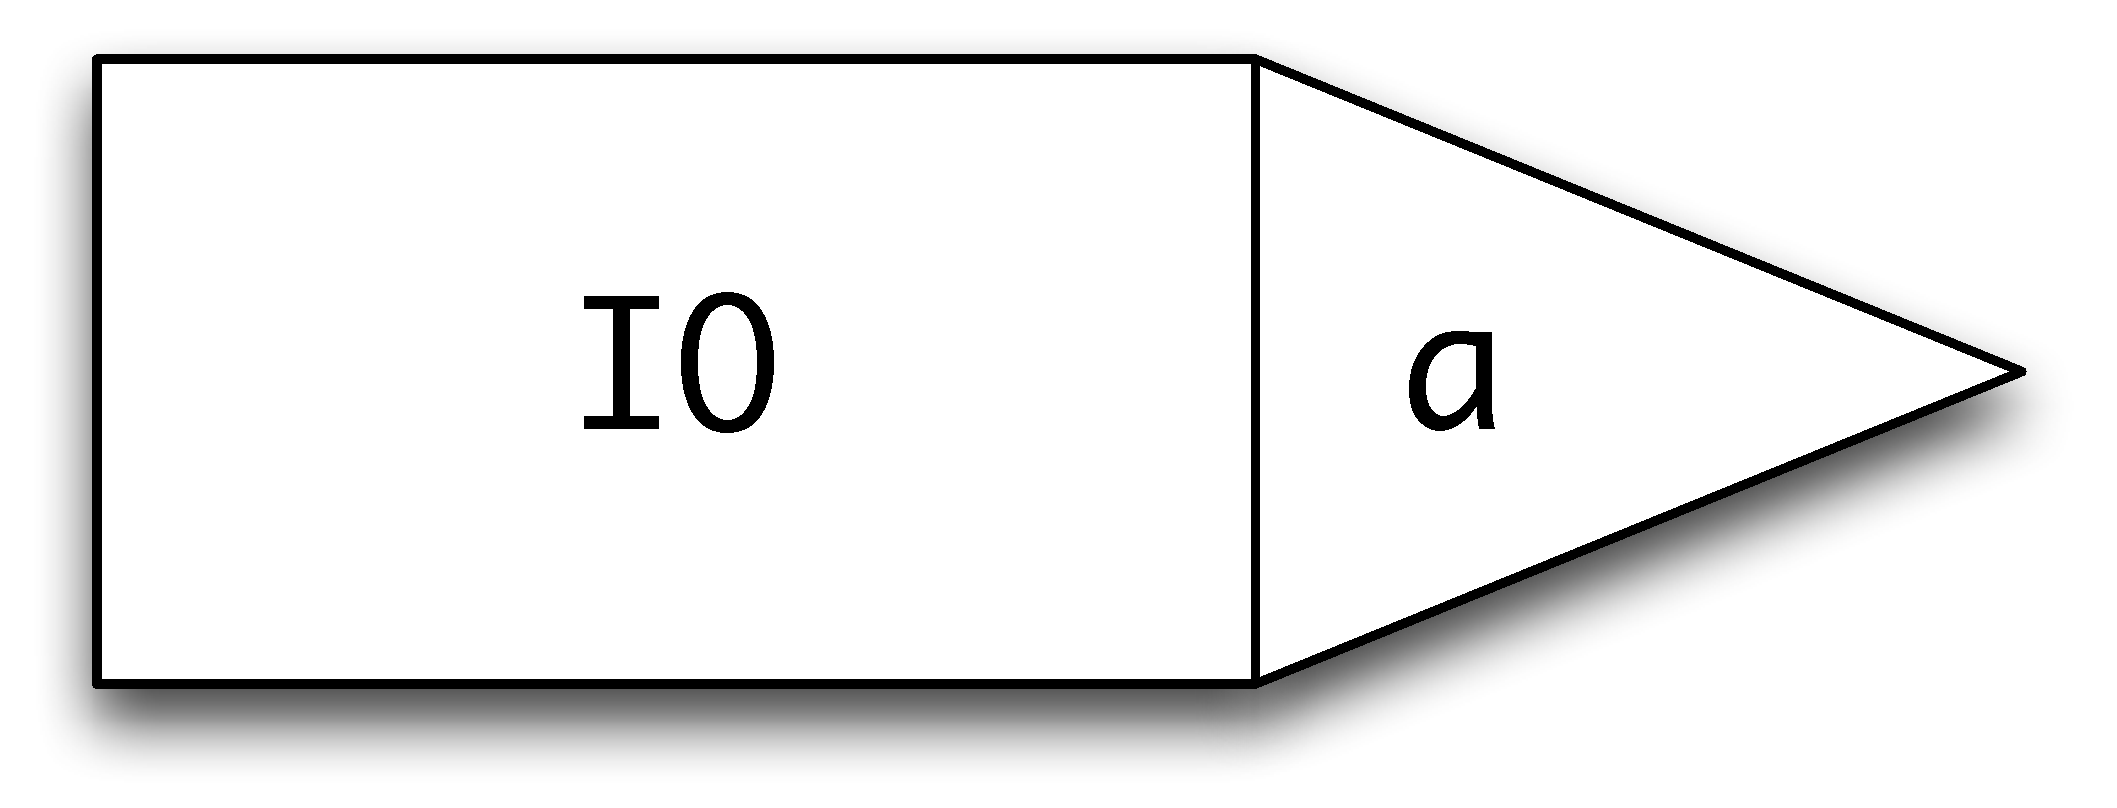
\includegraphics[height=1.2cm]{Pictures/Monad1.pdf}
\end{center}
with a \textbf{function}
taking the result of this (of type \texttt{a}) into an \texttt{IO b}, that is 
an object of type \texttt{a -> IO b},
\begin{center}

\includegraphics[height=1.2cm]{Pictures/Monad2.pdf}
\end{center}
We can join them together, passing the result of the first as an argument to
the second, thus:
\begin{center}
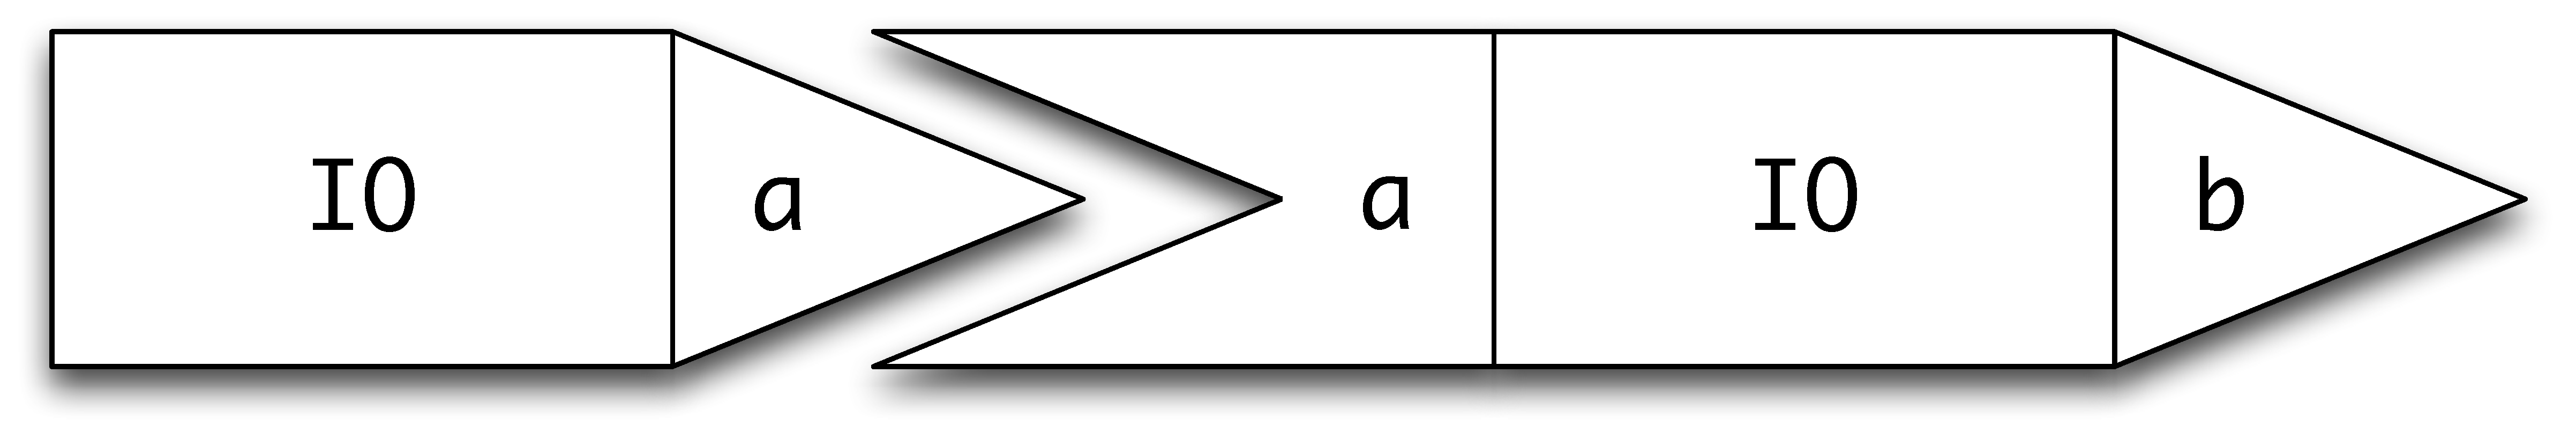
\includegraphics[height=1.2cm]{Pictures/Monad3.pdf}
\end{center}
The result of putting them together is something which does some I/O before
returning a value of type \texttt{b}:
\begin{center}
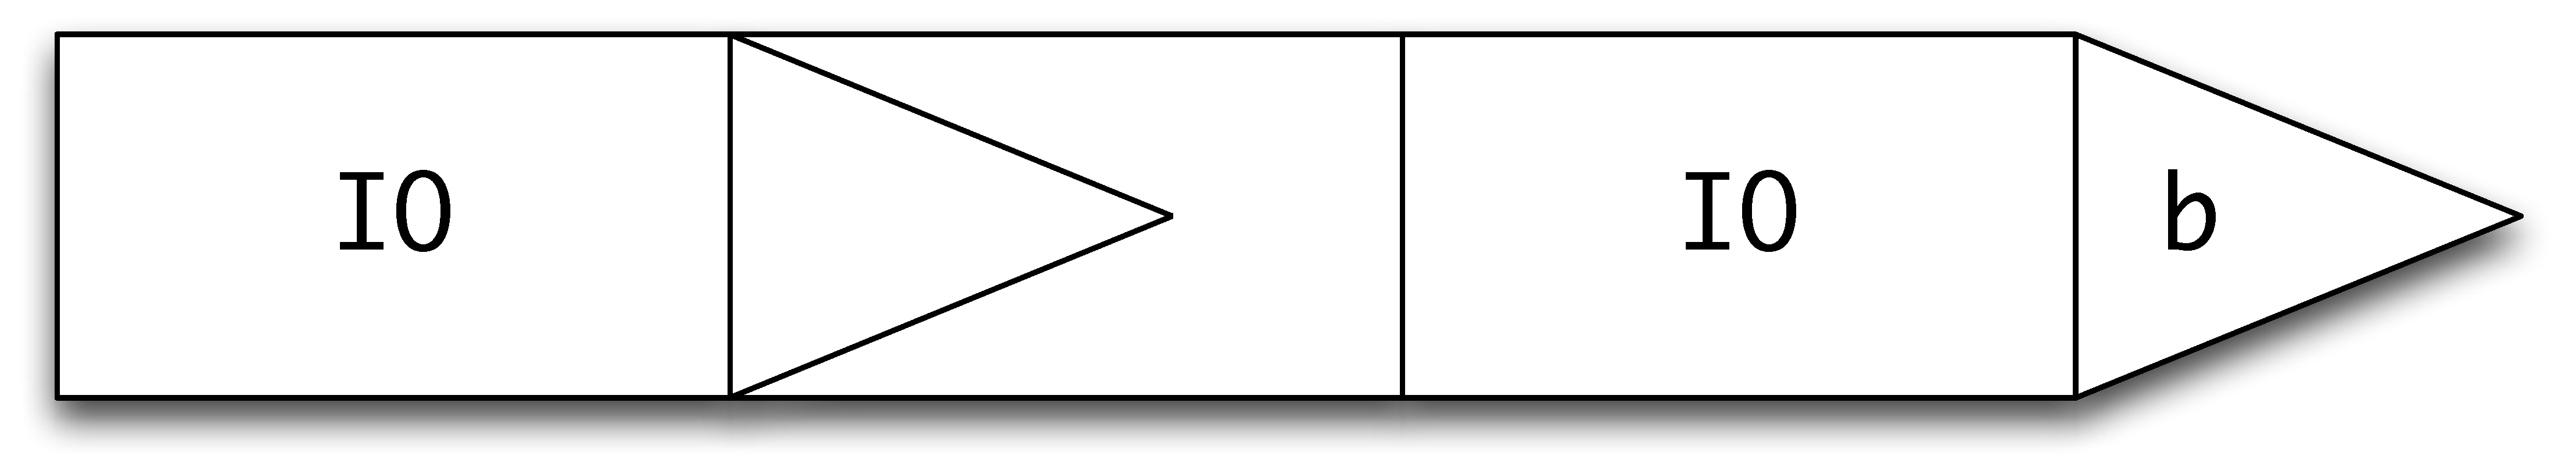
\includegraphics[height=1.2cm]{Pictures/Monad4.pdf}
\end{center}
in other words, an object of type \texttt{IO b}. 

How does this relate to
the \texttt{do} notation? The bind operation, \texttt{(>>=)}, is one of the simplest possible things we can define using \texttt{do}:
\begin{alltt}
m >>= f =
    do
      res <- m
      f res
\end{alltt}
First what we do is execute \texttt{m}, which is to type \texttt{IO a}, and name its result \texttt{res}; we then pass that to the function \texttt{f}, giving \texttt{f res} ,which is of type \texttt{IO b}.

In fact we can translate \emph{every} use of \texttt{do} into calls to \texttt{(>>=)}; \texttt{do} is just \emph{syntactic sugar} to make writing IO programs more readable.
Let's look at a particular example; consider what happens in the program
\begin{alltt}\minx{addOneInt}
addOneInt :: IO ()
addOneInt 
  = do line <- getLine
       putStrLn (show (1 + read line :: Int))       
\end{alltt}
The value returned by \texttt{getLine} is called \texttt{line} and then
used in the subsequent interaction. Using \texttt{(>>=)} we have to
sequence the interaction with a function expecting an argument of type
\texttt{String}, so we write
\begin{alltt}
addOneInt 
  = getLine >>= \bs{line} ->
    putStrLn (show (1 + read line :: Int))       
\end{alltt}
where recall that \texttt{\bs{x} -> e} is the function which takes the
parameter \texttt{x} to result \texttt{e}, so here the parameter is
called \texttt{line}, and used just as above. More complex examples
are translated in a similar way. 

As you can see from this simple example, using \texttt{(>>=)} makes programs more difficult to read and understand: the \texttt{do} notation highlights the essential features of I/O programming:
\begin{titemize}
\item sequencing operations, and,
\item binding the results of statements for use later on in the program.
\end{titemize}
and gives a readable and comprehensible way of writing these programs within Haskell.

We'll continue to use the
\texttt{do} notation, but will keep in mind that it essentially boils down to the existence of a
function \texttt{(>>=)} which does the work of sequencing I/O programs, and binding their results for future use.

\begin{exerciseone}
\item
Repeat some of the earlier examples and exercises using the \texttt{>>=}
operator instead of a \texttt{do} expression.
\index{I/O|)}
\end{exerciseone}

\section{Monads: languages for functional programming}
\label{monadFP}
\index{monad|(}


The \texttt{do} notation allows us to write \emph{programs} which perform I/O while calculating results; as we discussed in the last section, all we need to support the \texttt{do} notation is to have the `bind' function and `return' functions:
\begin{alltt}\minx{return}\index{\symbol{62}\symbol{62}\symbol{61}@\texttt{\symbol{62}\symbol{62}\symbol{61}}}
(>>=) :: IO a -> (a -> IO b) -> IO b
return :: a -> IO a
\end{alltt} 
The \texttt{IO} types give one kind of program which we can describe with the \texttt{do} notation, but there are other kinds of program we might want to write in a similar way, such as
\begin{titemize}
\item
programs that are \emph{non-deterministic}: we can think of these as programs which return a collection of results, as a list, say;
\item
programs that might give no answer at all;
\item
programs that work by manipulating a \emph{state}: that is programs that have variables in the sense of imperative languages like Java and C;
\item
programs that raise \emph{exceptions}, and can have those exceptions handled within the program.
\end{titemize}
Well, we \emph{can} do this, so long as the types have the analogue of the bind and return functions. In other words, we need to implement functions in a particular kind of \emph{interface}, and we know from Chapter \ref{classes} that this is given in Haskell by the \texttt{Monad} class, like this:
\begin{alltt}\minx{Monad}
class Monad m where
  (>>=)  :: m a -> (a -> m b) -> m b
  return :: a -> m a
\end{alltt}
Once we have an instance of this class we can use the \texttt{do} notation over the type. 

Let's look at the example of programs that might might give no answer, the second in the list of examples above. We looked at these in Section \ref{progErrs} where we saw that the \texttt{Maybe} type was a good model for values including a potentially absent result:
\begin{alltt}\minx{Maybe}\index{monad!\texttt{Maybe}}
data Maybe a = Nothing | Just a
\end{alltt}
and we developed a number of functions which worked with \texttt{Maybe} types to transmit errors through the code. Alternatively we can use the \texttt{do} notation, because we have this \texttt{instance} for \texttt{Monad}:
\begin{alltt}
instance Monad Maybe where
  (Just x) >>= k  =  k x
  Nothing  >>= k  =  Nothing
  return x        =  Just x
\end{alltt}
so that we get this behaviour using \texttt{do}:
\begin{alltt}
\textsl{Prelude>} do \{ x <- Just 1; y <- Just 2; return (x+y) \}
\textsl{Just 3}
\textsl{Prelude>} do \{ x <- Just 1; y <- Nothing; return (x+y) \}
\textsl{Nothing}
\textsl{Prelude>} do \{ x <- Nothing; y <- Just 2; return (x+y) \}
\textsl{Nothing}
\end{alltt}
where we are using the braces `\{', `\}' and explicit separator `:' to put the statements in the \texttt{do} program on a single line, as first introduced in Chapter \ref{writingProgs}. In a similar way, lists form a monad:
\begin{alltt}\index{monad!list}
instance Monad [] where
  xs >>= f  = concat (map f xs)
  return x  = [x]
\end{alltt} 
and we can use \texttt{do} notation over lists, like this:
\begin{alltt}
\textsl{Prelude>} do \{ x <- [1,2]; y <- [3,4]; return (x+y) \}
\textsl{[4,5,5,6]}
\end{alltt}
From this example we can see that lists model \emph{non-deterministic} computation: each of \texttt{x} and \texttt{y} have two possible values, and that gives four possibilities for \texttt{(x+y)}. The definition of \texttt{(>>=)} over lists reflects this: \texttt{f} is applied to all the possibilities in \texttt{xs} and the results are concatenated together.

In the next section we fill in some of the formalities about monads, but this latter section can be skipped on first reading, if you wish. We then look at some more examples of monads.

\beware{Why `monad'?}{\index{monad!terminology}
Why is this type class called `monad'? The name originates in category theory, which was used by Eugenio Moggi to build mathematical models of different kinds of computations. However, that doesn't mean that you need to learn category theory to use them, any more than you need to understand the intricacies of modern microprocessors to use your computer! Understanding that the \texttt{do} notation gives sequencing and binding (or naming) is all you need to understand to get started.}

\subsection*{Monads, formally}
\index{monad!definition}\minx{>>}

\index{\symbol{62}\symbol{62}\symbol{61}@\texttt{\symbol{62}\symbol{62}\symbol{61}}}
\minx{return}
A monad is a family of types \texttt{m a}, based on a polymorphic type
constructor \texttt{m}, with functions \texttt{return}, \texttt{(>>=)} and
\texttt{(>>)}:
\begin{alltt}
class Monad m where
  (>>=)  :: m a -> (a -> m b) -> m b
  return :: a -> m a
  (>>)   :: m a -> m b -> m b
\end{alltt}
This is an example of a \textbf{class}, whose instances are
\textbf{type constructors} -- that is functions which build types from
types -- rather than types. Examples of type constructors are `list',
written \texttt{[]} in Haskell, 
and \texttt{IO} as we have seen already.

The definition of \texttt{Monad} also contains a default declaration for \texttt{>>}:
\begin{alltt}
m >> k = m >>= \bs{}\_ -> k 
\end{alltt}
From this definition it can be seen that \texttt{>>} acts like \texttt{>>=}, except that the value
returned by the first argument is discarded rather than being passed to the second argument.

In order properly to be a monad, the functions \texttt{return} and \texttt{(>>=)}
should have some simple properties. Informally we can state the requirements
like this:
\begin{itemize}
\item
The operation \texttt{return x} should simply return the value
\texttt{x}, without any additional computational effect, such as input
or output in the case of the \texttt{IO} monad.
\item
The sequencing given by \texttt{>>=} should be irrelevant of the way
that expressions are bracketed.
\end{itemize}
The laws are much clearer when stated in terms of a derived operator,
\texttt{>=>}, prnounced `fish', that is defined in \texttt{Control.Monad}:
\index{\symbol{62}\symbol{64}\symbol{62}@\texttt{\symbol{62}\symbol{64}\symbol{62}}}
\begin{alltt}
(>=>) :: Monad m => (a -> m b) ->
                    (b -> m c) ->
                    (a -> m c)

f >=> g = \bs{x} -> (f x) >>= g
\end{alltt} 
This operator generalizes function composition\footnote{In category theory, this
operation is called \textbf{Kleisli composition}\index{Kleisli composition}.} \index{function composition}
in that it composes
objects 
\begin{center}

\includegraphics[height=1.2cm]{Pictures/Monad5.pdf}
\end{center}
to give
\begin{center}

\includegraphics[height=1.2cm]{Pictures/Monad6.pdf}
\end{center}
Note also that \texttt{return} is of this shape, as its type is
\texttt{a -> m a}. 

Now we can state formally the rules that the operations of
a monad should satisfy. \index{monad!properties}
First,
\texttt{return} is an \textbf{identity}\index{identity} for the operator \texttt{>=>}:
\begin{alltt}
return >=> f = f\hfill(M1)
f >=> return = f\hfill(M2)
\end{alltt}
and the operator \texttt{>=>} should be \textbf{associative}:\index{associativity}
\begin{alltt}
(f >=> g) >=> h = f >=> (g >=> h)\hfill (M3)
\end{alltt}
The derived sequencing operator, \texttt{>>}\minx{>>}, is also associative.

Of course, there is no way that we can make the requirements \texttt{(M1)}--\texttt{(M3)} 
a part of
the Haskell definition of \texttt{Monad}. 
We can also restate the rules in terms of
\texttt{do}, since, as we saw earlier,
\begin{alltt}
m >>= f  =  do \{ x <- m; f x \}
\end{alltt}
The first two rules become
\begin{alltt}
do \{ y <- return x; f y \} =  f x
do \{ x <- m; return x \}   =  m
\end{alltt}
and the third is implicit in the fact that the \texttt{do}
construct is associative.

\subsection*{Adding failure, \texttt{MonadFail}}
This type class adds a function marking that a computation has failed, \texttt{fail}, to an existing monad.
\begin{alltt}\minx{MonadFail}\minx{fail}
class Monad m => MonadFail m where
  fail   :: String -> m a
\end{alltt}
\item
The value \texttt{fail} \texttt{s} corresponds to a computation which
\textbf{fails}, giving the error message \texttt{s}. \index{monad!failure in (\texttt{fail})}

The definition of \texttt{MonadFail} also contains a default declaration for \texttt{fail}
\begin{alltt}
fail s = error s
\end{alltt}

\begin{exercises}
 

\item
Show that lists and the \texttt{Maybe} type are instances of \texttt{MonadFail}. Hint: in both cases the \texttt{String} argument is ignored.

\item
Once a computation has failed, it cannot be ``unfailed'' as it were. As a law this is expressed as \texttt{fail s >>= f  =  fail s}. Show that this rule holds for the instances of \texttt{MonadFail} that you defined in the previous exercise.


\end{exercises}

\subsection*{Some more examples}
\index{monad!examples}

Now we have seen the definition of what it means to be a monad, with or without failure, we look at some more examples of monads in Haskell.



\subsubsection*{The parsing monad}
\index{parsing!monad}
\index{monad!parsing}


A more substantial example is given by parsing, where we can show that
\texttt{Parse a} is a monad. To make a formal declaration of this we
need to wrap it in a \texttt{newtype} constructor, \texttt{MP},
which clutters the definition a bit.
\begin{alltt}
newtype MP a b = MP \{ mp :: (Parse a b) \}

instance Monad (MP a) where
  return x = MP (succeed x)
  (MP pr) >>= f 
    = MP (\bs{st} -> concat [ mp (f x) rest | (x,rest) <- pr st ])

instance MonadFail (MP a) where
  fail s   = MP none
\end{alltt}
The crux of the definition of \texttt{(>>=)} is like that of
\texttt{(>*>)} -- a parse is done by one parser, \texttt{pr}, and the remains of the
input are passed to a second parser \texttt{f}, here dependent on the result of the
first parse, and so a result of the first parse, \texttt{x}, is passed
to \texttt{f} to give a second parser, which is applied to the remaining
input, \texttt{rest}.

How does the monadic approach to parsing look in practice? Let's go back to the calculator example, and in particular the definition of \texttt{opExpParse} in Section \ref{parsing}, page \pageref{opExpParse}. If we redefine it monadically, we get
\begin{alltt}
opExpParseM :: MP Char Expr
opExpParseM =
    do
      tokenM '('
      e1 <- parseExprM 
      bop <- spotM isOp
      e2 <- parseExprM
      tokenM ')'
      return (Op (charToOp bop) e1 e2)
\end{alltt}
where \texttt{tokenM} is the monadic equivalent of \texttt{token}, and so forth. How do the definitions differ? It is mainly in the handling of the results: in the earlier treatment we built the results into a nested tuple, gathering a result for each step whether or not we needed it, and then passed the tuple to a function, via \texttt{build}. The approach here has the advantage that
\begin{titemize}
\item
we only name the results of the sub-parses that we need, and
\item
we can build the final result directly, using these names, rather than having to use a function to re-jig the tuple into the value we want.
\end{titemize} 
The disadvantage of the non-monadic approach is reminiscent of the discussion of `point-free' programming on page \pageref{pointfree}: under both we combine functions, when the judicious use of names (of variables, of intermediate results) make the program substantially easier to read, write and understand.

\subsubsection*{The identity monad}
\index{monad!identity}

The identity monad, which takes a type to itself, is the simplest
example of a monad, with the definitions
\begin{alltt}
x >>= f = f x 
return = id
\end{alltt}
In order for this to be a legal Haskell definition we need to define the identity type constructor, and, within Haskell 2010, any instance declaration needs to be for a \texttt{data} type, \texttt{newtype} or primitive type. So, we define, as in \texttt{Control.Monad.Identity},   
\begin{alltt}
newtype Identity a = Identity { identity :: a }
\end{alltt}
where the constructor \texttt{Identity} `wraps' the value up, and the field name, \texttt{identity} is used to `unwrap' them.. Now we can define the instance itself,
\begin{alltt} 
instance Monad Identity where
    (Identity x) >>= f = f x          --  x >>= f = f x 
    return a           = Identity a   --  return = id 
\end{alltt}
We can then run things in this monad, if we give a \texttt{Show} instance for \texttt{Identity}
\begin{alltt}
instance Show a => Show (Identity a) where
    show (Identity x) = show x
\end{alltt}
as in this example, which also shows how we can give multi-line input to GHCi interactively.
\begin{alltt}
\textsl{*UseMonads>} :\{
\textsl{*UseMonads}| do \{ x <- return 'c' :: Identity Char;
\textsl{*UseMonads}|      y <- return 'd';
\textsl{*UseMonads}|      return [x,y] \}
\textsl{*UseMonads}| :\}
\textsl{"cd"}
\end{alltt}
Computationally, this monad represents the trivial state in which no
actions are performed, and values are returned immediately.




\subsubsection*{The state monad}
\index{monad!state}

Later in this chapter we will give an example of a \textbf{state} monad, 
\texttt{State a b}. An operation of this type can change the state (of type 
\texttt{a}) before returning
a value of type \texttt{b}.





\subsection*{Some standard functions and the \texttt{Functor} class}

There is a set of standard functions over monads, defined in \texttt{Control.Monad}; we just look at two of these here. Their types should be
familiar from the list case
\begin{alltt}\minx{fmap}\minx{join}
fmap :: Monad m => (a -> b) -> m a -> m b
join :: Monad m => m (m a) -> m a
\end{alltt}
and their definitions are
\begin{alltt}
fmap f m 
  = do x <- m 
       return (f x)
join m  
  = do x <- m
       x
\end{alltt}
Over lists these functions are called \texttt{map} and \texttt{concat};
many of the properties of \texttt{map} and \texttt{concat} over lists lift to these
functions. For instance, we can show using properties \texttt{(M1)} to \texttt{(M3)}
that for all \texttt{f} and \texttt{g}
\begin{alltt}
fmap (f.g) = fmap f . fmap g\hfill(M4)
\end{alltt}
In fact, \texttt{fmap} is defined over a wider set of types that monads, and it is the function that characterises the \texttt{Functor}\minx{Functor} class that we saw earlier:
\begin{alltt}
class Functor f where
  fmap :: (a -> b) -> f a -> f b
\end{alltt}
Example instances of \texttt{Functor} which are not monads include \texttt{(a,a)}, \texttt{([a],[a])} and \texttt{Tree a} (from the next section).

\begin{exercises}

\item
Show that sets and binary trees
can be given a monad structure, as can the type:
\begin{alltt}
data Error a = OK a | Error String
\end{alltt}

\item
For the monads \texttt{Id} , \texttt{[]} and \texttt{Maybe} prove the rules 
\texttt{(M1)} to \texttt{(M3)}. Also show that
these rules hold for your implementations in the
previous exercise.

\item
Prove the property \texttt{(M4)} using the laws \texttt{(M1)} to \texttt{(M3)}.

\item 
Prove the following properties using the monad laws:
\begin{alltt}
join . return = join . fmap return
join . return = id
\end{alltt}

\item
Can you define a different monad structure over lists from that given above?
Check that your definition has properties \texttt{(M1)} to \texttt{(M3)}.

\item
Write down the definitions of \texttt{map} and \texttt{join} over lists
using list comprehensions. Compare them with the definitions of
\texttt{fmap} and \texttt{join} given in the \texttt{do} notation in this section.

\item
Re-implement the parser for the calculator using the \texttt{do}
construct (based on \texttt{>>=}) 
rather than \texttt{(>*>)} and \texttt{build}. Contrast the two
approaches.

\item
Show that the type functions \texttt{(a,a)}, \texttt{([a],[a])} and \texttt{Tree a} are instances of \texttt{Functor}.

\end{exercises}

\section{Example: monadic computation over trees}
\index{monad!trees}
\label{monadicTrees}

We now illustrate how computations over the type of 
\begin{alltt}
data Tree a = Nil | Node a (Tree a) (Tree a)\minx{Tree}
\end{alltt}
can be given a monadic structure. We first look at a simple example, and then
we look at a rather more realistic one. 

We see that with a monadic approach the top-level
structure of the two solutions 
is exactly the same. This structure guides the way that we build the
implementation of the second example, as we shall see.

The moral of these examples is
that monads provide an important structuring mechanism for program
construction, as they encourage a \textbf{separation of concerns}. The
top-level structure of the computation is given in terms of a
monad whose specific properties are only touched upon. Within the monad itself
is the appropriate computational behaviour to, for example, 
maintain a state or to perform some
IO (or both); the particular sequencing operation of the monad will
ensure that values are passed between the parts of the program in an
appropriate way.

This separation of concerns comes into its own when changes are required
in the details of the computation: it is usually possible to change the monad
implementing a computation with at most minimal changes required at the
top level. This is in stark contrast to a non-monadic computation in
which data representations are visible: a wholesale restructuring is
often required in such a situation.

\subsection*{Summing a tree of integers}

Suppose we are asked to give the sum of a tree of integers,
\begin{alltt}
sTree :: Tree Integer -> Integer
\end{alltt}
A direct recursive solution is
\begin{alltt}\minx{sTree}
sTree Nil            = 0
sTree (Node n t1 t2) = n + sTree t1 + sTree t2
\end{alltt}
In writing this we give no explicit sequence to the calculation of the sum: we
could calculate \texttt{sTree t1} and \texttt{sTree t2} one after the other, or
indeed in parallel. How might a monadic solution proceed?
\begin{alltt}
sumTree :: Tree Integer -> St Integer\minx{sumTree}
\end{alltt}
where \texttt{St} is a monad which we have yet to define. In the \texttt{Nil} case,
\begin{alltt}
sumTree Nil = return 0
\end{alltt}
while in the case of a \texttt{Node} we calculate the parts in a given order:
\begin{alltt}
sumTree (Node n t1 t2)\hfill(sumTree)\label{sumTree}
  = do num <- return n
       s1  <- sumTree t1
       s2  <- sumTree t2
       return (num + s1 + s2)
\end{alltt}
How is the definition structured? We put the operations in sequence, using
\texttt{do}. First we \texttt{return} the value \texttt{n}, giving it the 
name \texttt{num}. Next we calculate \texttt{sumTree t1} and \texttt{sumTree t2}, naming 
their results \texttt{s1} and \texttt{s2}. Finally we \texttt{return} the result, which
is the sum \texttt{num+s1+s2}. 

Now, since all we are doing here is calculating values and not trying to do
any I/O or other side-effecting operation, we make the monad 
\texttt{St} the {\em identity\/} monad \texttt{Identity} which we mentioned
earlier, so we have
\begin{alltt}
sumTree :: Tree Integer -> Identity Integer
\end{alltt}
There is a similarity between the definition \texttt{(sumTree)} and an
imperative program, bearing in mind that \texttt{do} performs a sequencing and
\texttt{j <- ...} gives (or assigns) a value to \texttt{j}. In an imperative
setting, we might well write 
\begin{alltt}
num := n ;
s1  := sumTree t1 ;
s2  := sumTree t2 ;
return (num + s1 + s2) ;
\end{alltt}
where `\texttt{num :=}' corresponds to the `\texttt{<-}' and \texttt{do} puts a 
sequence of commands one after the other, as does the semi-colon. Remember, though, that this is a \emph{single-assignment} language, so that \texttt{num}, \texttt{s1} and so on are names not variables!
\index{monad!and imperative programming}
\index{imperative programming!and monads}

To give a function of type \texttt{Tree Integer -> Integer} we compose with the
\texttt{identity} function to give
\begin{alltt}
identity . sumTree
\end{alltt}
where
\begin{alltt}
identity :: Identity a -> a
identity (Identity x) = x
\end{alltt}
takes the wrapper off an element \texttt{Identity x} to give the element
\texttt{x}.
In the next section we tackle a more complex problem, but see the same monadic
structure repeated.

\subsection*{Using a state monad in a tree calculation}
\index{monad!state}

Building on the experience of the last section in defining \texttt{sumTree} we
tackle here a rather more tricky problem. We want to write a function
\begin{alltt}
numTree :: Eq a => Tree a -> Tree Integer
\end{alltt}
so that given an arbitrary tree we transform it to a tree of integers in which
the original elements are replaced by natural numbers, starting from \texttt{0}.
An example is given in Figure \ref{treeTrans}.
The same element has to be replaced by the same number at every occurrence,
and when we meet an as-yet-unvisited element we have to find a `new' number to
match it with.

\begin{figure}[t]
\begin{center}
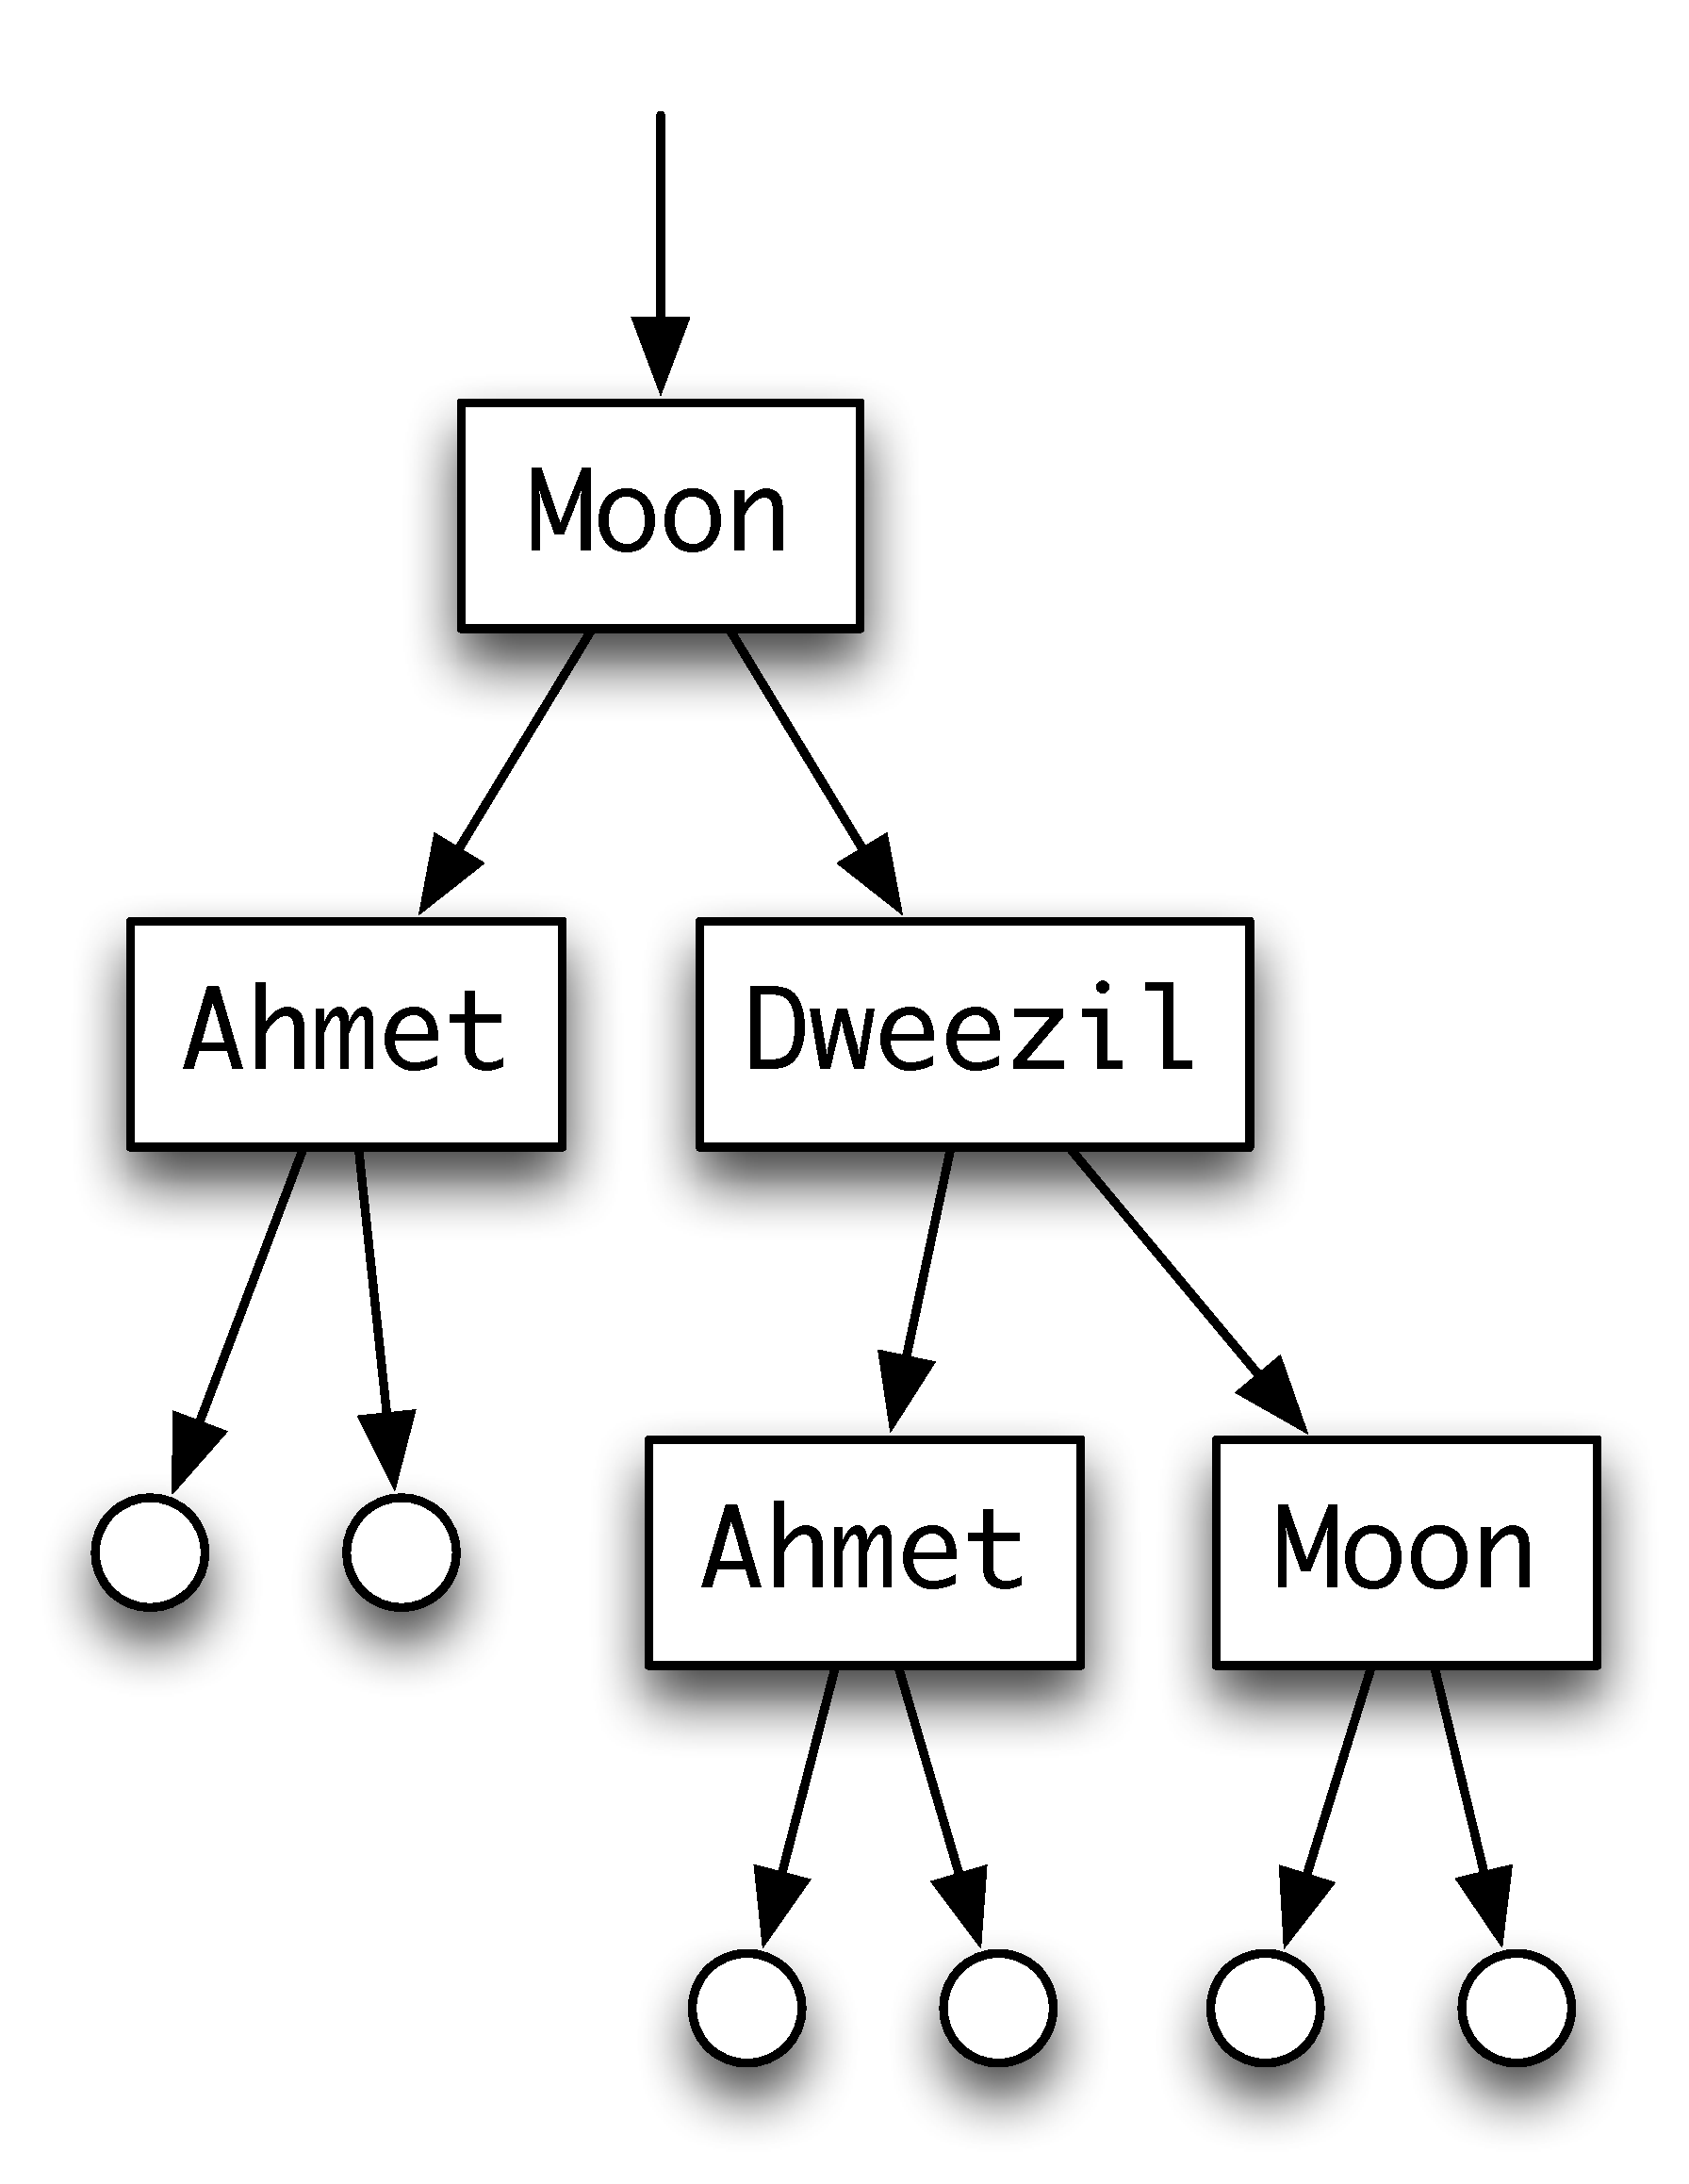
\includegraphics[height=6cm]{Pictures/TreeBefore.pdf}\hspace*{1cm}
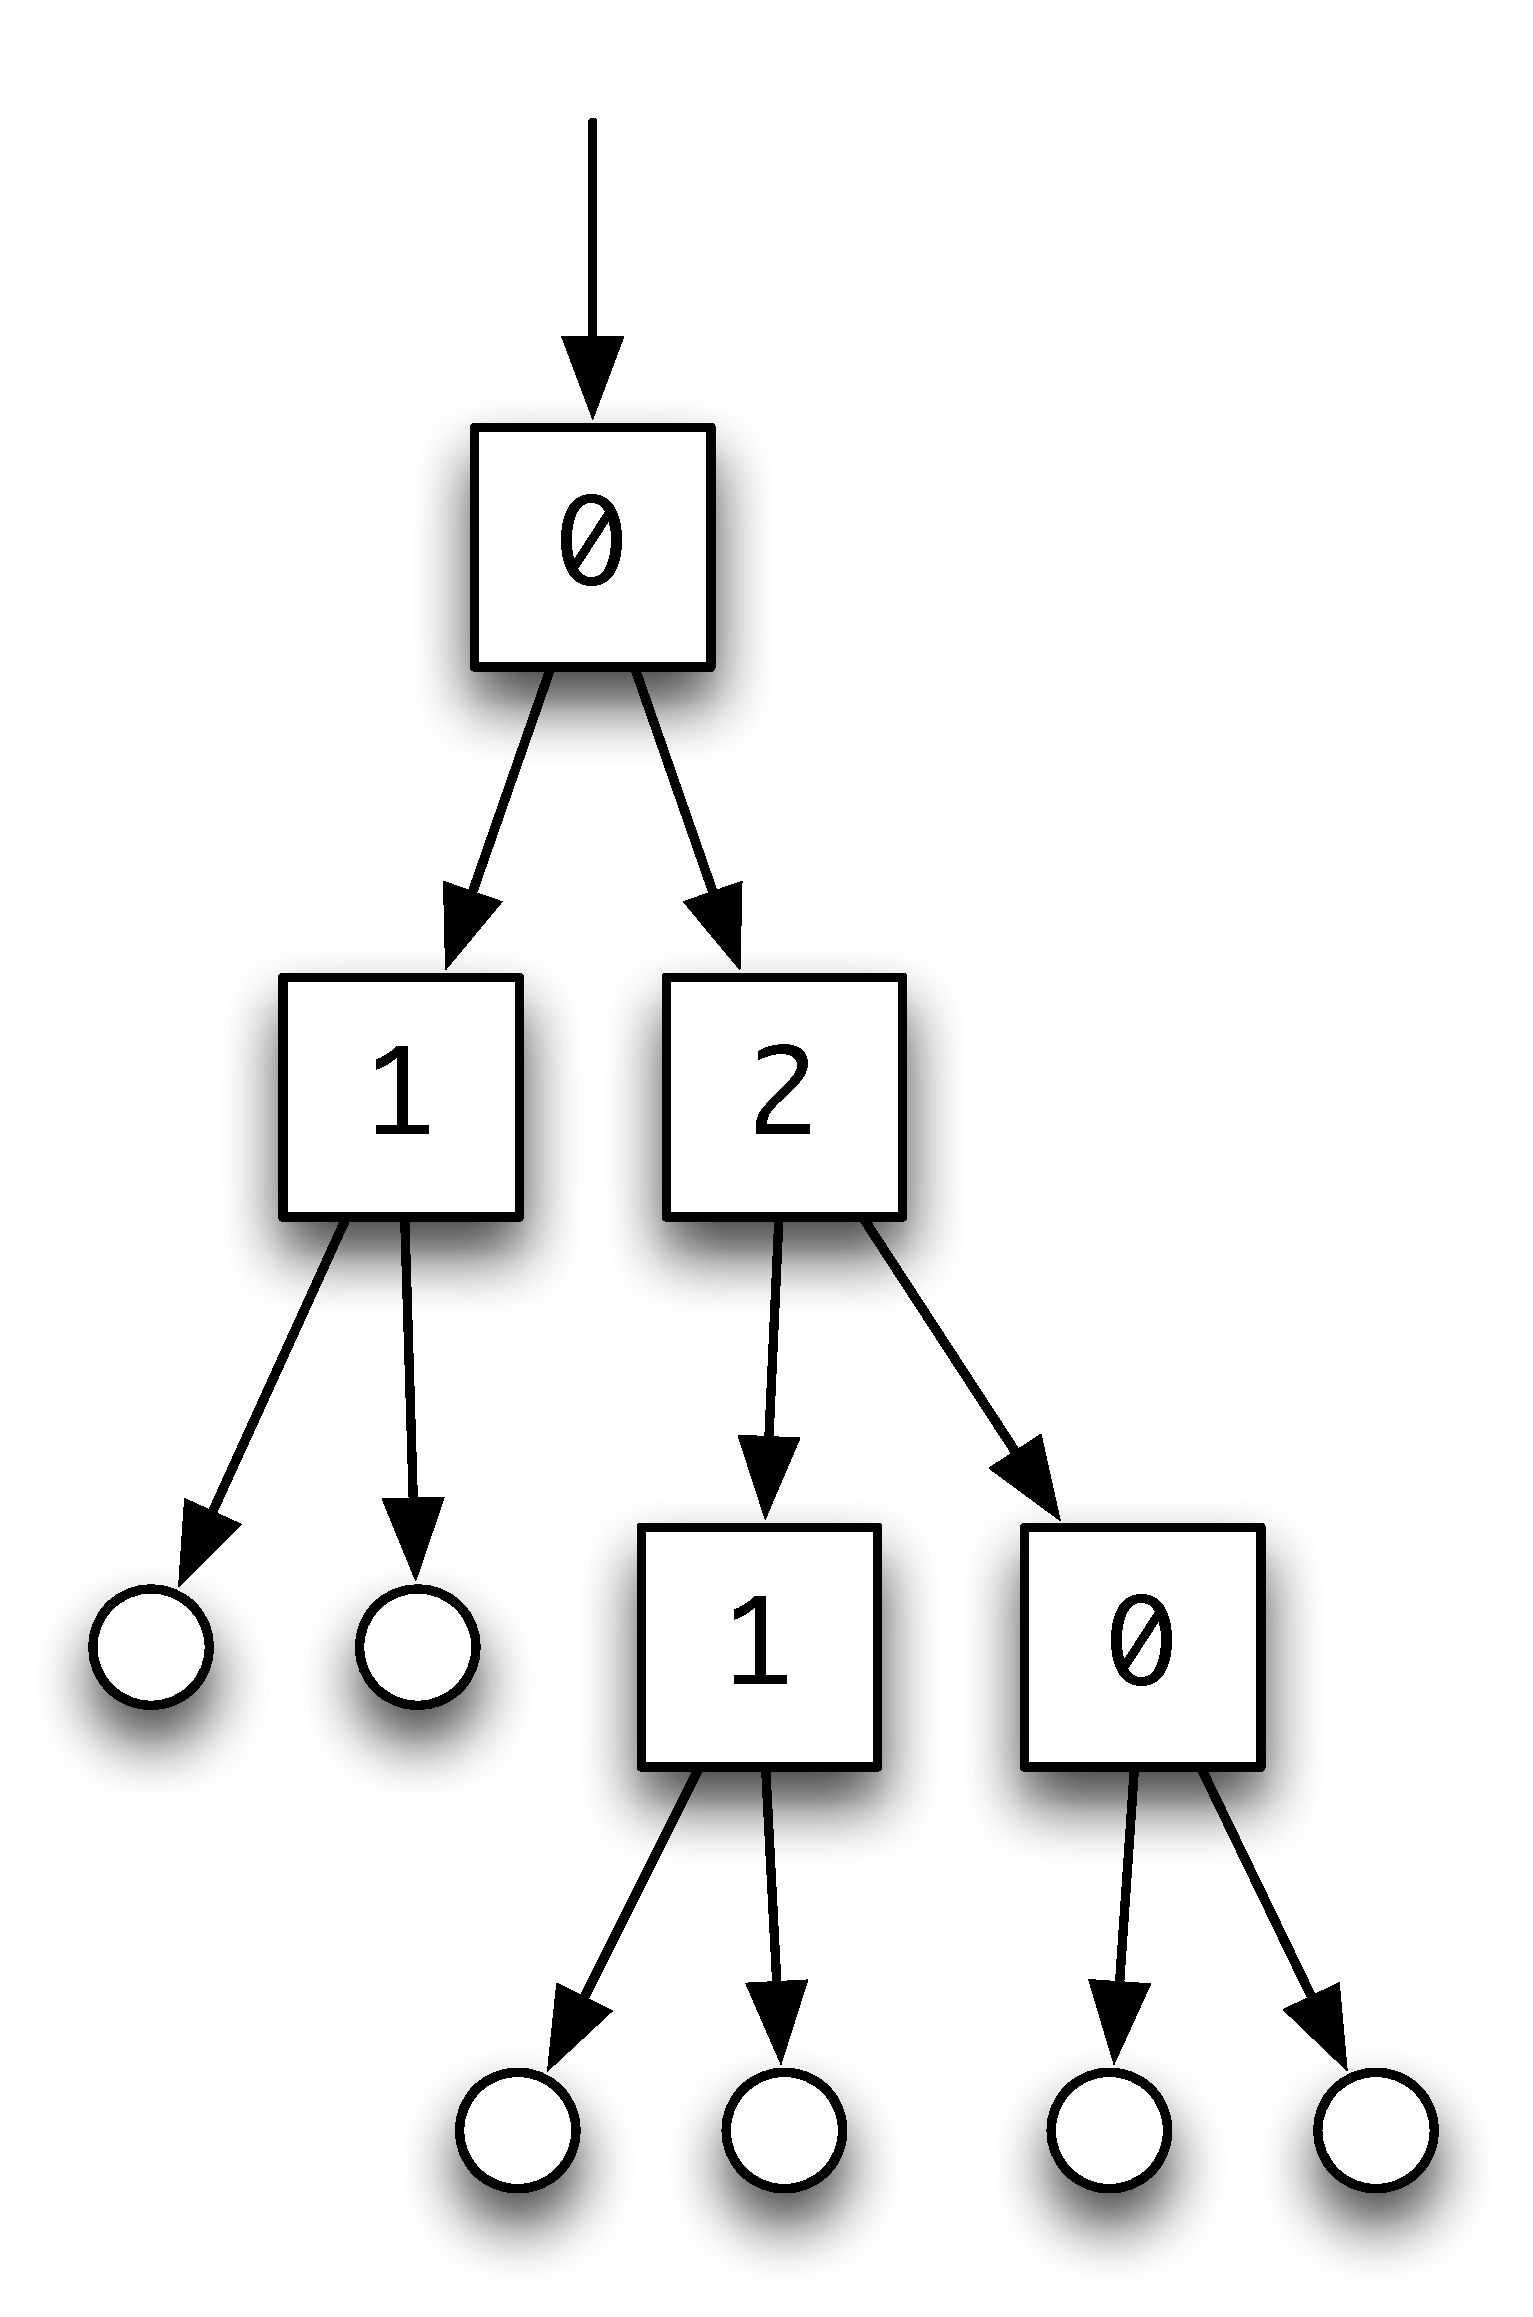
\includegraphics[height=6cm]{Pictures/TreeAfter.pdf}
\end{center}
\caption{Replacing the elements of a tree with natural numbers.}
\label{treeTrans}
\end{figure}

\subsubsection*{Describing the calculation}


How does our definition appear? We give the function a type,
\begin{alltt}\minx{numberTree}
numberTree :: Eq a => Tree a -> State a (Tree Integer)
\end{alltt}
in which the monad \texttt{State a} will have to carry about enough information
to allow us to replace the elements in the correct way. The structure of the
program then is
\begin{alltt}
numberTree Nil = return Nil

numberTree (Node x t1 t2)\hfill(numberTree)
  = do num <- numberNode x
       nt1 <- numberTree t1
       nt2 <- numberTree t2
       return (Node num nt1 nt2)
\end{alltt}
The structure here is exactly the same as that of \texttt{(sumTree)} on
page \pageref{sumTree}; we perform
the operations on the components \texttt{x}, \texttt{t1} and \texttt{t2} (for the
subtrees we use recursion) and then combine them in the result 
\texttt{(Node num nt1 nt2)}.

What else do we have to define to give the result? We need to identify the
monad \texttt{State a} and to define the function which replaces an individual
\minx{State}
entry, 
\begin{alltt}
numberNode :: Eq a => a -> State a Integer
\end{alltt}
We now have to think about the implementation of the monad. We have called it
\texttt{State} since it keeps a record of the state, that is of which values are
associated with which numbers. This we do in a table:
\begin{alltt}\minx{Table}
type Table a = [a]
\end{alltt}
where the table \texttt{[True,False]} indicates that \texttt{True} is associated
with \texttt{0} and \texttt{False} with \texttt{1}.

\subsubsection*{The \texttt{State} monad}

What then is the state monad? It consists of functions
\begin{alltt}\minx{State}
data State a b = State (Table a -> (Table a , b))
\end{alltt}
which, after we strip off the constructor \texttt{State},
we can think of as taking the state {\em before\/} doing the operation
to the state {\em after\/} the operation, together with its result. In other
words, we return a value of type \texttt{b}, but perhaps we change the value of
the state of type \texttt{Table a} as a side-effect.

Next we have to define the two monad operations.
\begin{alltt}
instance Monad (State a) where
\end{alltt}
To \texttt{return} a value, we leave the state
unchanged.
\begin{alltt}\minx{return}
  return x = State (\bs{t}ab -> (tab,x))
\end{alltt}
How do we sequence the operations?
The intended effect here is to do \texttt{st}, pass its result to \texttt{f}
and then do the resulting operation.

In more detail, to perform \texttt{st}, we pass it the table \texttt{tab}; the output of this is a
new state, \texttt{newTab}, and a value \texttt{y}. This \texttt{y} is passed to 
\texttt{f}, giving an object of type \texttt{State~a~b}; this is then performed starting
with the {\em new\/} state \texttt{newTab}. 
\begin{alltt}\index{\symbol{62}\symbol{62}\symbol{61}@\texttt{\symbol{62}\symbol{62}\symbol{61}}}
  (State st) >>= f 
    = State (\bs{t}ab -> let 
                     (newTab,y)    = st tab
                     (State trans) = f y 
                     in
                     trans newTab)
\end{alltt}
Here we can see that the operations are
indeed done in sequence, leading from one state value to the next.

\subsubsection*{Completing the definition}


This has given us the monad; all that remains is to define the function 
\texttt{numberNode}. Our definition is
\begin{alltt}\minx{numberNode}
numberNode :: Eq a => a -> State a Integer
numberNode x = State (nNode x)

nNode :: Eq a => a -> (Table a -> (Table a , Integer))
nNode x table
  | elem x table        = (table      , lookup x table)
  | otherwise           = (table++[x] , integerLength table)
    where
    integerLength = toInteger.length
\end{alltt}
If \texttt{x} is an element of \texttt{table}, we return its position in the table,
given by \texttt{lookup}; if it is not, we add it to the end of the table, and
return its position, which is the length of the table. The definition
of 
\begin{alltt}
lookup :: Eq a => a -> Table a -> Integer
\end{alltt}
is standard, and we leave it as an exercise for the reader.

\subsubsection*{Running the program}

Standing back, we can see that we have completed our definition of the
function
\begin{alltt}
numberTree :: Eq a => Tree a -> State a (Tree Integer)
\end{alltt}
but one ingredient of the solution is still needed. If we form
\begin{alltt}
numberTree exampleTree
\end{alltt}
for some \texttt{exampleTree} of the tree type, we have an object in 
\begin{alltt}
State a (Tree Integer)
\end{alltt}
In order to \emph{extract} the result of running the program, we have to write a function
\begin{alltt}
runST :: State a b -> b
\end{alltt}
This has to perform the calculation, starting with some initial table, and
return the resulting value of type \texttt{b}. The definition is
\begin{alltt}
runST :: State a b -> b
runST (State st) = snd (st [])
\end{alltt}
where we see that \texttt{st} is applied to the initial state \texttt{[]}. The result
of this is a pair, from which we select the second part, of type \texttt{b}.
Now we can define our function
\begin{alltt}
numTree :: Eq a => Tree a -> Tree Integer
numTree = runST . numberTree
\end{alltt}
which has the effect we require.

\subsubsection*{Discussion}


To conclude, we have shown how a complex calculation over a tree, 
\texttt{(numberTree)}, can be structured in exactly the same way as a simple one, 
\texttt{(sumTree)}. In the case of a tree type the advantage is tangible, but for more
complex types a monadic structure becomes almost essential if we are to follow
a computation with complicated side-effects. 

To see how much the monadic approach has tidied up the computation, it's interesting to see what the computation would look like if we passed the state around explicitly. Each function would need to take a `before' state as part of its input, and return an `after' state as part of its result. We'd then have to thread state values through the functions so that state is updated as we compute. With the monadic approach, all the explicit threading is in the definition of \texttt{(>>=)} and the rest is given by the \texttt{do} notation.

\beware{The \texttt{Control.Monad.State} module}{\minx{Control.Monad.State}
What we have presented here gives the essential idea behind the state monad in Haskell. The monad contained in \texttt{Control.Monad.State} is more complicated than the version presented here; our simplified version still gives the essential idea of a monad which threads state through a calculation.
}

\subsection*{Taking it further}\index{monad!further reading}

What we have presented here just scratches the surface of monadic programming in Haskell. We have covered the basic monads, but not looked how multiple monads -- such as state and exceptions -- can be combined into a single monad: this is done using \emph{monad transformers}, for which a number of libraries are available.

We have also not looked in any detail at monadic approaches to \emph{parsing}, beyond showing how our earlier, non-monadic, parser combinators could support a monadic view too. Most of the available Haskell parsing libraries -- which extend the basic approach in both expressivity and efficiency -- are monadic.

There are extensions to the \texttt{Monad} interface: many monads, including lists and the \texttt{Maybe} monad, have a natural notion of a sum and zero: this gives the \texttt{MonadPlus} interface. At the same time, there are various weakenings of the notion of monad, including applicative functors and arrows, each with their own advantages and disadvantages.

There is no shortage of online tutorials on monads and these other features, and other texts cover them in more detail too. A standout among these is Peyton Jones' tutorial \cite{awkwardSquad} on the `awkward squad' of monads that support IO, exceptions and other computational effects.







\index{monad|)}

\begin{exercises}

\item
Give a non-monadic definition of \texttt{numTree}, threading the state through the computation explicitly; compare your solution with the monadic version given here.

\item 
Show how to look up the position of an element in a list
\begin{alltt}
lookup :: Eq a => a -> Table a -> Int
\end{alltt}
You might find it useful to define a function
\begin{alltt}
look :: Eq a => a -> Table a -> Int -> Int
\end{alltt}
where the extra integer parameter carries the current `offset' into the list.

\item
Show how you can use a \texttt{State}-style monad in a computation to replace
each element in a tree by a random integer, generated using the techniques of
Section \ref{infLists}.

\item
We can use monads to extend the case study of the calculator in a variety of
ways. Consider how you would
\begin{titemize}
\item add exceptions or messages to be given on an attempt to divide by zero;
\item count the number of steps taken in a calculation; and
\item combine the two.
\end{titemize}

\end{exercises}



\begin{summary}%
\index{design!monads and}%
\index{monad!advantages of monads}%

In this chapter we have seen how the \texttt{do} notation, which we first saw used for I/O programming, can be used to support a whole lot of different kinds of program: non-deterministic, stateful, parsing and so on. The mechanism which underlies the \texttt{do} notation is the \texttt{Monad} class, which embodies the functionality needed to sequence sub-programs, and to name their results for use later on in the program.

Like any abstract data type interface, the advantage of programming against the interface is that it is possible to modify the underlying implementation without changing the higher-level program. We saw this in action in the final section of the chapter, where two very different computations over a tree had the same top-level structure, described in a monad.

We will come back to monads in the next chapter, where we look at how Haskell is a host for `little languages' that describe how to compute in a particular application area.

\index{actions|)}

\end{summary}

%\end{document}

%\documentclass{book}\usepackage{sjtfonts}\usepackage{includegraphics}\usepackage{alltt}\usepackage{latexsym}
%\usepackage{array}
%\begin{document}\input{defs0}%		miradefs.tex 		    June 1994

% opening and closing a quoted Miranda section

\newcommand{\mira}{\noindent\hrulefill\nopagebreak\so}
\newcommand{\arim}{\nopagebreak\st\hrulefill\\}

% backslash in the Miranda environment
% Only feasible approach is to use \verb+\+
% in line!

%\newcommand{\bs}{$\mi\backslash\!\!$}
%\newcommand{\lbs}{\mbox{\verb+\+}}

% ignoring part of the input

\newcommand{\ignore}[1]{}

% a blank line in a Miranda section

\newcommand{\bl}{\mbox{\ }}

% Signalling a diffculty.

\definecolor{light-gray}{gray}{0.95}

\newcommand{\beware}[2]
 {\medskip\noindent\colorbox{light-gray}{\parbox{\textwidth}
 {\mbox{\large\textbf{#1}} \medskip\noindent\\ #2}\medskip\noindent}}

% Subscripting in Miranda text
\newcommand{\subscr}[2]{\mbox{${\mbox{\texttt{#1}}}_{\mbox{\texttt{#2}}}$}}

%\newcommand{\subscr}[2]{\mbox{${\mbox{\mi #1}}_{\mbox{\smtt #2}}$}}
\newcommand{\aone}{\subscr{a}{1}}
\newcommand{\atwo}{\subscr{a}{2}}
\newcommand{\ak}{\subscr{a}{k}}

\newcommand{\aoneone}{\subscr{a}{1,1}}

\newcommand{\eone}{\subscr{e}{1}}
\newcommand{\etwo}{\subscr{e}{2}}
\newcommand{\ei}{\subscr{e}{i}}
\newcommand{\er}{\subscr{e}{r}}

\newcommand{\fone}{\subscr{f}{1}}
\newcommand{\fl}{\subscr{f}{l}}

\newcommand{\gone}{\subscr{g}{1}}
\newcommand{\gtwo}{\subscr{g}{2}}
\newcommand{\gi}{\subscr{g}{i}}
\newcommand{\gr}{\subscr{g}{r}}

\newcommand{\hone}{\subscr{h}{1}}
\newcommand{\hl}{\subscr{h}{l}}

\newcommand{\pone}{\subscr{p}{1}}
\newcommand{\ptwo}{\subscr{p}{2}}
\newcommand{\pk}{\subscr{p}{k}}

\newcommand{\qone}{\subscr{q}{1}}
\newcommand{\qtwo}{\subscr{q}{2}}
\newcommand{\qk}{\subscr{q}{k}}

\newcommand{\rone}{\subscr{r}{1}}
\newcommand{\rtwo}{\subscr{r}{2}}

\newcommand{\tone}{\subscr{t}{1}}
\newcommand{\ttwo}{\subscr{t}{2}}
\newcommand{\tn}{\subscr{t}{n}}

\newcommand{\vone}{\subscr{v}{1}}
\newcommand{\vtwo}{\subscr{v}{2}}
\newcommand{\vn}{\subscr{v}{n}}

% for regular expressions

\newcommand{\stone}{\subscr{st}{1}}
\newcommand{\sttwo}{\subscr{st}{2}}
\newcommand{\stn}{\subscr{st}{n}}
\newcommand{\rthree}{\subscr{r}{3}}

\newcommand{\eps}{$\varepsilon$}
\newcommand{\trans}[1]{\stackrel{\mbox{\tt #1}}{\longrightarrow}}



% superscript in Miranda text

\newcommand{\superscr}[2]{\mbox{${\mbox{\mi #1}}^{\mbox{\smtt #2}}$}}

% Not equals in Miranda text

\newcommand{\noteq}{\makebox[0pt][l]{=}/}
\newcommand{\overslash}{\makebox[0pt][l]{/}}

% Definitions in complexity chapter

\newfont{\oldSym}{cmsy10}
\newcommand{\Th}{\boldmath$\oldSym\Theta$}
\newcommand{\pow}[1]{\^{}#1}
\newcommand{\leqq}{$\leq$}
\newcommand{\geqq}{$\geq$}
\newcommand{\lll}{$\ll$}
\newcommand{\eqq}{$\equiv$}
\newcommand{\ltwo}{\subscr{log}{2}}

% Indexing

\newcommand{\minx}[1]{\index{#1@{\ttfamily{}#1}}}
\setcounter{chapter}{18}\setcounter{page}{1001}


\chapter{Time and space behaviour}
\chapstart
\label{behaviour}
\index{behaviour|(}

\newcommand{\up}[1]{\ensuremath{{}^{\mbox{\footnotesize\texttt #1}}}}

This chapter explores not the values which programs compute, but the way in
which those values are reached; we are interested here
in program \emph{efficiency} rather than program correctness. 

We begin our
discussion by asking how we can measure complexity in general, before
asking how we measure the time and space behaviour of our functional programs.
We work out the time complexity of a sequence of functions, leading up to
looking at various implementations of the \texttt{Set} abstype.

The \emph{space} behaviour of lazy programs is complex: we show that some
programs use less space than we might predict, while others use more. This
leads into a discussion of folding functions into lists, and we
introduce the \texttt{foldl'} function, which folds from the left, and gives more
space-efficient versions of folds of operators which need their arguments --
the \emph{strict} operations. In contrast to this, \texttt{foldr} gives better
performance on lazy folds, in general.

In many algorithms, the naive implementation causes recomputation of  parts
of the solution, and thus a poor performance. In the final section of the
chapter we show how to exploit lazy evaluation to give more efficient
implementations, by \emph{memoizing} the partial results in a table.

\section{Complexity of functions}
\index{complexity|(}
\label{funComplex}

If we are trying to measure the behaviour of functions, one approach is to ask
how much time and space are consumed in evaluations for different
input values. We might, for example, given a function \texttt{fred} over the
natural numbers, count the number of steps taken in calculating the value of
\texttt{fred n} for natural numbers \texttt{n}. This gives us a function, call it
\texttt{stepsFred}, and then we can ask how complex that function is. 

One way of estimating the complexity of a function is to look at how fast it
grows for large values of its argument. The idea of this is that the essential
behaviour of a function becomes clearer for large values. To start with, we examine this idea 
through an example.
How fast does the function
\begin{alltt}
f n = 2*n\up{2} + 4*n + 13
\end{alltt}
grow, as \texttt{n} gets large? The function has
three components:
\begin{titemize}
\item a constant \texttt{13}, 
\item a term \texttt{4*n}, and 
\item a term, \texttt{2*n\up{2}}. (Note that here we use the mathematical
notation for powers, \texttt{n\up{2}}, rather than the Haskell notation,
\texttt{n\pow{2}}.)
\end{titemize}
As the values of \texttt{n} become large, how do these components behave?
\begin{titemize}
\item The constant \texttt{13} is unchanged; 
\item the term \texttt{4*n} grows like a straight line; but 
\item a square term, \texttt{2*n\up{2}}, will grow the most quickly.
\end{titemize}
For `large' values of \texttt{n} the square term is greater than the others, and
so we say that \texttt{f} is of \textbf{order} \index{order}
\texttt{n\up{2}}, \texttt{O(n\up{2})}. In this
case the square dominates for any \texttt{n} greater than or equal to \texttt{3}; we
shall say exactly what is meant by `large' when we make the definition of
order precise. As a rule of thumb we can say that order classifies how
functions behave when all but the fastest-growing
components are removed, and constant
multipliers are ignored; the remainder of the section makes this precise, but
this explanation should be sufficient for understanding the remainder of the
chapter.

The notation \texttt{n\up{2}} is the usual way that mathematicians write down
`the function that takes \texttt{n} to \texttt{n\up{2}}'. This is the notation which
is generally used in describing complexity, and so we use it here. In
a Haskell program to describe the function we would either
write \texttt{\bs{n} -> n\pow{2}} or use the operator section
\index{operator sections}
\texttt{(\pow{2})}.

In the remainder of this section we make the idea of order precise, before
examining various examples  and placing them on a scale for measuring
complexity.

\subsection*{The `big-Oh' and Theta notation -- upper bounds}
\index{+@\texttt{O}}
\index{+@\texttt{\Th}}
A function \texttt{f ::\ Integer -> Integer} is \texttt{O(g)} -- pronounced `{\em big-Oh} \texttt{g}' -- if
there are positive integers \texttt{m} and \texttt{d}, so that for all 
\texttt{n\geqq{}m},
\begin{alltt}
f n \leqq\ d*(g n)
\end{alltt}
The definition expresses the fact that when numbers are large enough
(\texttt{n\geqq{}m}) the value of \texttt{f} is no larger than  a multiple
of the function \texttt{g}, namely \texttt{(d*).g}. 

For example, \texttt{f} above is \texttt{O(n\up{2})} since, for \texttt{n} greater than
or equal to \texttt{1},
\begin{alltt}
2*n\up{2} + 4*n + 13 \leqq\ 2*n\up{2} + 4*n\up{2} + 13*n\up{2} = 19*n\up{2} 
\end{alltt}
so the definition is satisfied by taking \texttt{m} as 
\texttt{1} and \texttt{d} as \texttt{19}.

Note that the measure gives an upper bound, which may be an overestimate; by
similar reasoning, \texttt{f} is \texttt{O(n\up{17})} as well. In most cases we 
consider
the bound will in fact be a tight one. One way of expressing that \texttt{g} is
a tight bound on \texttt{f} is that in addition to \texttt{f} being \texttt{O(g)},
\texttt{g} is \texttt{O(f)}; we then say that \texttt{f} is \texttt{\Th(g)} -- pronounced `{\em Theta}
\texttt{g}' -- our example \texttt{f} is in fact \texttt{\Th(n\up{2})}.

\ignore{

\subsubsection*{The Theta notation -- tight bounds}

A function \texttt{f ::\ Integer -> Integer} is \texttt{\Th(g)}, {\em Theta} \texttt{g}, if
there are positive integers \texttt{m}, \texttt{c}  and \texttt{d}, so that for all 
\texttt{n\geqq{}m},
\begin{alltt}
c*(g n) \leqq\ f n \leqq\ d*(g n)
\end{alltt}
Our example \texttt{f} is in fact \texttt{\Th(n\up{2})}, as if we choose \texttt{c} to
be \texttt{2}, and keep \texttt{d} and \texttt{m} as the same values, for all 
\texttt{n\geqq{}1},
\begin{alltt}
2*n\up{2} \leqq\ 2*n\up{2} + 4*n + 13
\end{alltt}
It is {\em not\/} the case that \texttt{f} is \texttt{\Th(n\up{17})}.
} % end ignore

\subsection*{A scale of measurement}

We say that \texttt{f \lll\ g} \minx{\lll}
if \texttt{f} is \texttt{O(g)}, but \texttt{g} is 
\texttt{not\/} \texttt{O(f)}; we also use \texttt{f \eqq\ g} to mean that \texttt{f} is  
\texttt{O(g)} and simultaneously \texttt{g} is \texttt{O(f)}. 

We now give a scale by which function complexity can be measured.
Constants which are
\texttt{O(n\up{0})} grow more slowly than \textbf{linear} -- \texttt{O(n\up{1})} --
\index{complexity!linear}
functions,
which in turn grow more slowly than \textbf{quadratic} 
\index{complexity!quadratic}
functions  of order \texttt{O(n\up{2})}.
This continues through the powers, and all the powers \texttt{(n\up{k})} are bounded
by exponential functions, such as \texttt{2\up{n}}.

\begin{alltt}
n\up{0} \lll\ n\up{1} \lll\ n\up{2} \lll\ \ldots\ \lll\ n\up{k} \lll\ \ldots\ \lll\ 2\up{n} \lll\ \ldots
\end{alltt}
Two other points ought to be added to the scale. The logarithm function, \texttt{log}, grows more slowly 
than any positive power, and the product of the functions 
\texttt{n} and \texttt{log n},  
\texttt{n(log n)} fits between linear and quadratic, like this:
\begin{alltt}
n\up{0} \lll\ log n \lll\ n\up{1} \lll\ n(log n) \lll\ n\up{2} \lll\ \ldots
\end{alltt}

\subsection*{Counting}
\index{counting}
\label{counting}

Many of the arguments we make will involve counting. In this section we look at
some general examples which we will come across in examining the behaviour of
functions below.
\begin{example}
\subexample*{1.}\index{lists!bisection of}
The first question we ask is -- given a list, how many times can we \textbf{bisect} it,
before we cut it into pieces of length one? If the length is \texttt{n}, after
the first cut, the length of each half is \texttt{n/2}, and after \texttt{p} cuts,
the length of each piece is \texttt{n/(2\up{p})}. This number will be smaller
than or equal to one when 
\begin{alltt}
(2\up{p}) \geqq\ n > (2\up{(p-1)})
\end{alltt}
which when we take \texttt{\subscr{log}{2}} of each side gives
\begin{alltt}
p \geqq\ \subscr{log}{2} n > p-1
\end{alltt}
The function giving the number of steps in terms of the length of the
list, \texttt{n},
will thus be \texttt{\Th(\subscr{log}{2} n)}.


\subexample*{2.}
The second question concerns trees. A tree is called \textbf{balanced}
\index{tree!balanced}\index{tree!branch length}
if all its branches are the same length. Suppose we have a balanced binary
tree, whose branches are of length \texttt{b}; how many nodes does the tree
have? 
\begin{figure}[t]
\begin{center}
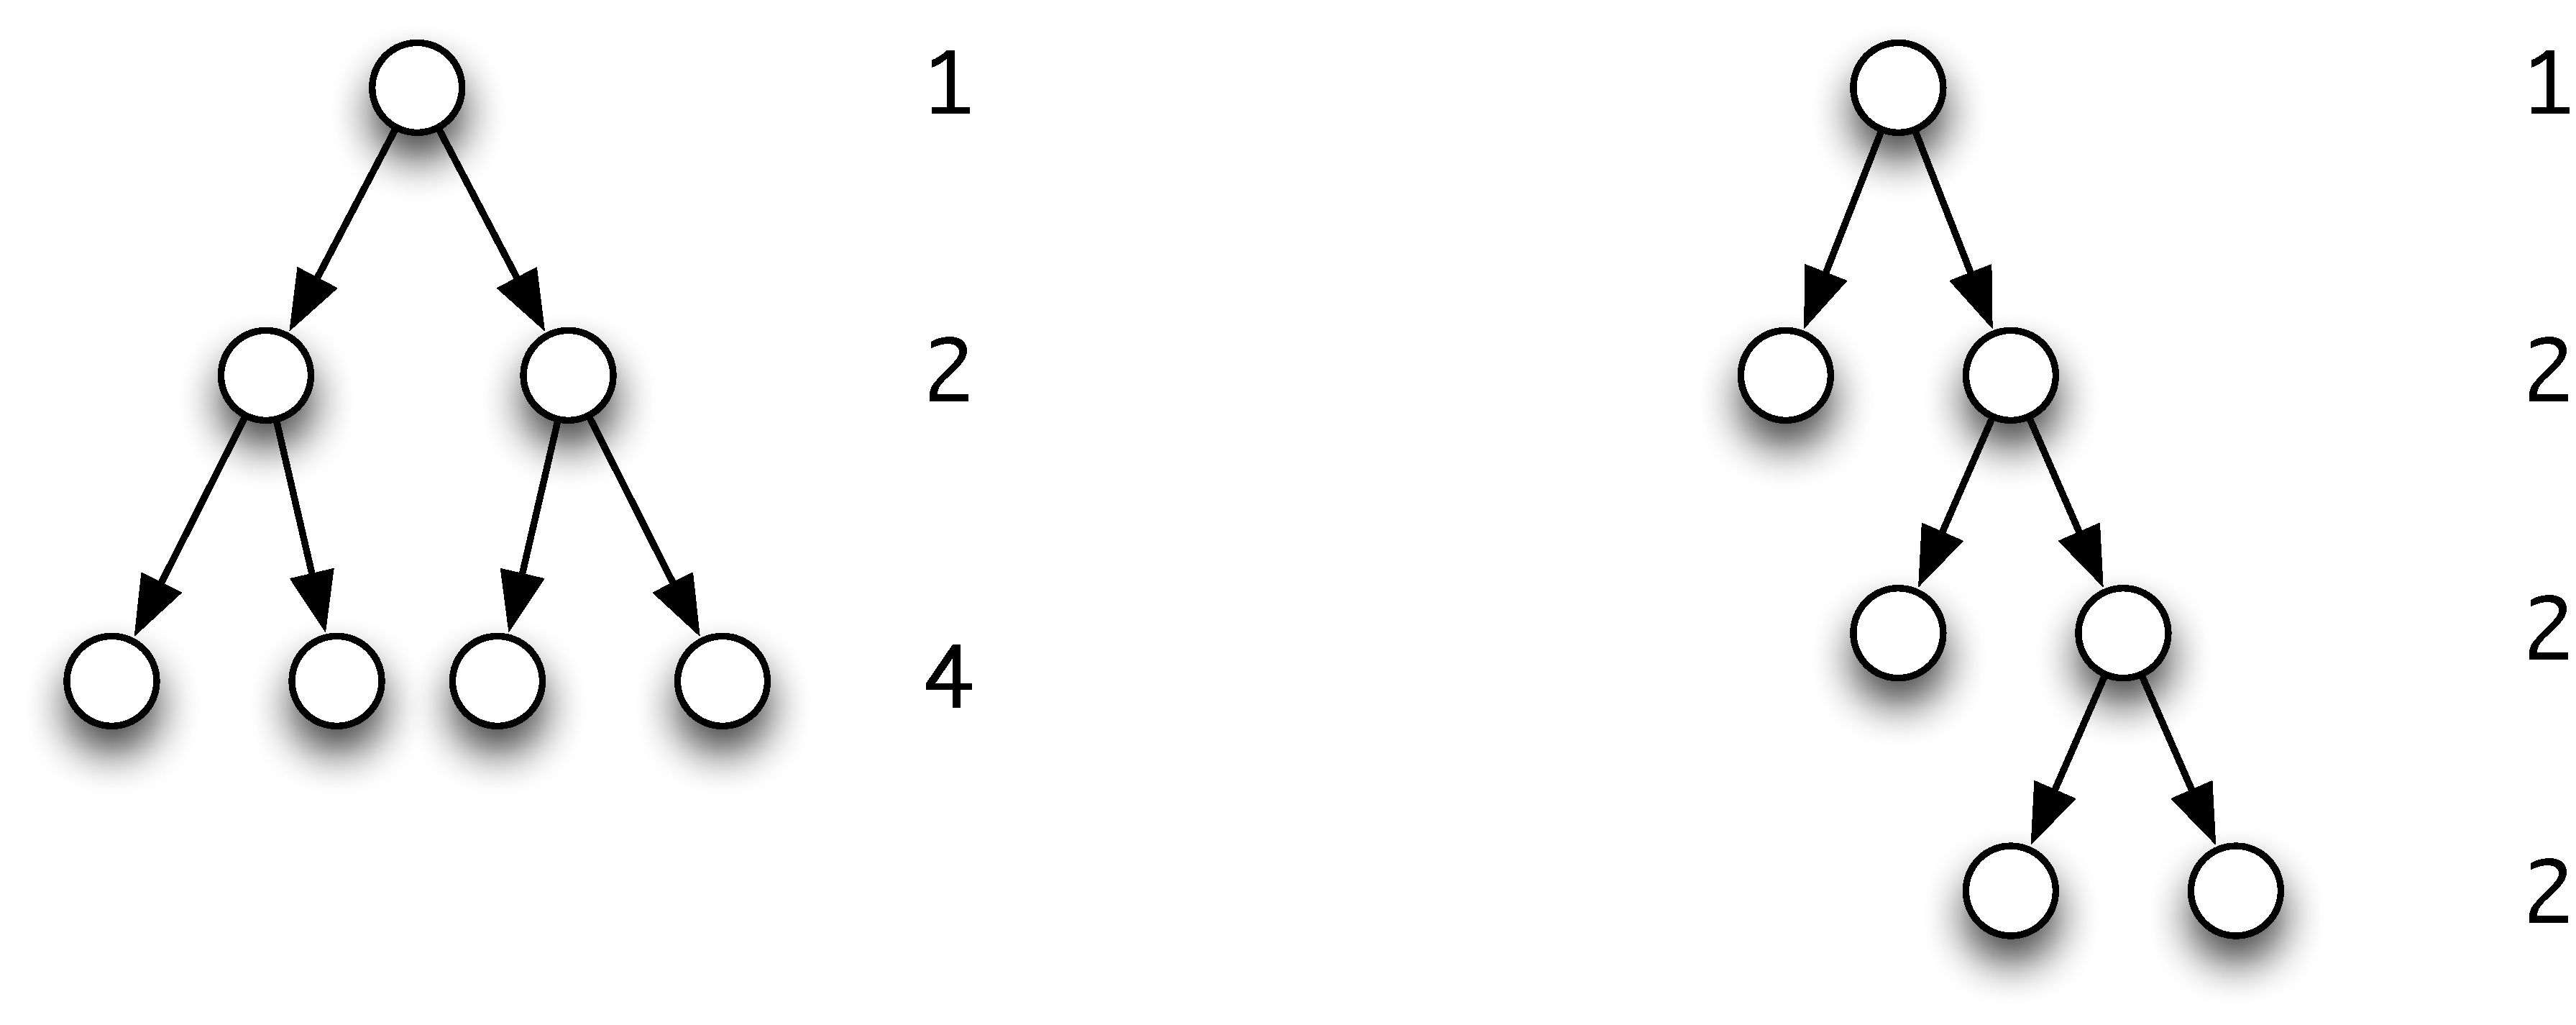
\includegraphics[width=3in]{Pictures/CountTrees.pdf}
\end{center}
\caption{Counting the number of nodes of trees.}
\label{countTrees}
\end{figure}
On the first level it has \texttt{1}, on the
second \texttt{2}, on the \texttt{k}th it has \texttt{2\up{(k-1)}}, so over all 
\texttt{b+1} levels it has
\begin{alltt}
1 + 2 + 4 + \ldots + 2\up{(k-1)} + \ldots + 2\up{b} = 2\up{(b+1)} - 1
\end{alltt}
as illustrated in Figure \ref{countTrees}.

We thus see that the size of a balanced tree is
\texttt{\Th(2\up{b})} in the length of the branches, \texttt{b}; taking logarithms, a
balanced tree of size \texttt{n} will therefore have branches of length 
\texttt{\Th(\ltwo\ n)} in the size of the tree. If a tree is not balanced, the
length of its longest branch can be of the same order as the size of the tree
itself; see Figure \ref{countTrees} for an example. 


\subexample*{3.}
Our final counting question concerns taking \textbf{sums}. If we are given one object
every day for \texttt{n} days, we have \texttt{n} at the end; if we are given 
\texttt{n} each day, we have \texttt{n\up{2}}; what if we are given \texttt{1} on the
first day, \texttt{2} on the second, and so on? What is the sum of the list 
\texttt{[1 ..\ n]}, in other words? Writing the list backwards, as well as forwards, we
have
\begin{alltt}
1     + 2     + 3     +  ...  + (n-1) + n +
n     + (n-1) + (n-2) +  ...  + 2     + 1 
\end{alltt}
adding {\em vertically\/} at each point we have a sum of \texttt{(n+1)}, 
\begin{alltt}
(n+1) + (n+1) + (n+1) +  ...  + (n+1) + (n+1)
\end{alltt}
and this
sum occurs \texttt{n} times, so 
\begin{alltt}
sum [1 ..\ n] = n*(n+1) `div` 2
\end{alltt}
which makes it 
\texttt{\Th(n\up{2})}, or quadratic. In a similar way, the sum of the squares is
\texttt{\Th(n\up{3})}, and so on.
 \end{example}


\begin{exercises}

\item
Show that the example
\begin{alltt}
f n = 2*n\up{2} + 4*n + 13
\end{alltt}
is \texttt{\Th(n\up{2})}.

\item
Give a table of the values of the functions \texttt{n\up{0}}, \texttt{log n}, 
\texttt{n\up{1}}, \texttt{n(log n)}, \texttt{n\up{2}}, \texttt{n\up{3}} and 
\texttt{2\up{n}} for the values 
\begin{alltt}
0 1 2 3 4 5 10 50 100 500 1000 10000 100000 10000000
\end{alltt}

\item
By giving the values of \texttt{d}, \texttt{m} and \texttt{c} (when necessary), show
that the following functions have the complexity indicated.
\begin{alltt}
f1 n = 0.1*n\up{5} + 31*n\up{3} + 1000              O(n\up{6})
f2 n = 0.7*n\up{5} + 13*n\up{2} + 1000              \Th(n\up{5})
\end{alltt}

\item
Show that \texttt{n\up{k} \lll\ 2\up{n}} for all positive \texttt{k}. By taking
logarithms of both sides, show that \texttt{log n \lll\ n\up{k}} for all
positive \texttt{k}.

\item
Show that 
\begin{alltt}
log \eqq\ ln \eqq\ \ltwo
\end{alltt}
and in fact that logarithms to any base have the same rate of growth.

\item
The function \texttt{fib} is defined by
\begin{alltt}
fib 0 = 0
fib 1 = 1
fib m = fib (m-2) + fib (m-1)
\end{alltt}
Show that \texttt{n\up{k}\ \lll\ fib n} for all \texttt{k}.

\item
Show that \texttt{\lll} is transitive -- that is \texttt{f\lll{}g} and 
\texttt{g\lll{}h} together imply that \texttt{f\lll{}h}. Show also that \texttt{\eqq} is an
equivalence relation.

\item
If \texttt{f} is \texttt{O(g)}, show that any constant multiple of \texttt{f} is also
of the same order. If \texttt{f1} and \texttt{f2} are \texttt{O(g)}, show that their
sum and difference are also \texttt{O(g)}. Are the same results valid
with \texttt{\Th} replacing \texttt{O}?

\item
If \texttt{f1} is \texttt{O(n\up{k1})} and \texttt{f2} is \texttt{O(n\up{k2})}, show
that their product,
\begin{alltt}
f n = f1 n * f2 n
\end{alltt}
is  \texttt{O(n\up{(k1+k2)})}.

\item
Prove by induction over the natural number \texttt{n} that
\begin{alltt}
1 + 2 + 4 + \ldots + 2\up{n} = 2\up{(n+1)} - 1
1 + 2 + \ldots + n      = n*(n+1) `div` 2
1\up{2} + 2\up{2} + \ldots + n\up{2}   = n*(n+1)*(2*n+1) `div` 6
1\up{3} + 2\up{3} + \ldots + n\up{3}   = (n*(n+1) `div` 2)\up{2}
\end{alltt}
\end{exercises}



\section{The complexity of calculations}
\label{complexCalc}

How can we measure the complexity of the functions we write? One answer is to
use an implementation of Haskell, which can be expected to produce some
diagnostic information about evaluation. We examine this option in Section \ref{foldingRev}, page \pageref{perfInPractice}, but for the moment we opt for a cleaner \emph{model} of what is going on, and we
choose to analyse the \emph{calculations} we have been using. There are
three principal measures we can use.
\begin{titemize}
\item The \textbf{time} taken to compute a result is given by the number
of steps in a calculation which uses lazy evaluation.
\index{behaviour!time}\index{complexity!time}
\item The \textbf{space} necessary for the computation can be
\index{behaviour!space}\index{complexity!space}
measured in two ways.
First, there is a lower limit on the amount of space we need for a calculation
to complete successfully. During calculation, the expression
being calculated grows and shrinks; obviously, we need enough
space to hold the {\em largest\/} expression built during the calculation.
This is often called the \textbf{residency}\index{residency} of the computation, we shall call
it the \textbf{space complexity}.
\item We can also make a measure of the
\textbf{total space} used by a computation, which in some way reflects the total
area of the calculation; it is of interest to implementers of functional
languages  but for users (and for us) the first two are the crucial measures.
\end{titemize}
How then do we measure the complexity of a function?

\subsection*{Complexity measures}

We measure the complexity of the function \texttt{f} by looking at the time and
space complexity as described above, as {\em functions\/} of the {\em size\/}
of the inputs to \texttt{f}. The size of a number is the number itself, while
the size of a list is given by its length, and of a tree by the number of
nodes it contains. We now look at a series of examples.
\begin{example}
\subexample*{1.}\index{complexity!\texttt{fac}}
Let us start with the example of \texttt{fac}.\minx{fac}
\begin{alltt}
fac :: Integer -> Integer
fac 0 = 1
fac n = n * fac (n-1)
\end{alltt}
Working through a calculation, we have
\begin{alltt}
fac n
\step n * fac (n-1)
\step ...
\step n * ((n-1) * ... * (2 * (1 * 1)) ...) \hfill (facMax)
\step n * ((n-1) * ... * (2 * 1) ...) 
\step n * ((n-1) * ... * 2 ...)  
\step ...
\step n!
\end{alltt}
The calculation contains \texttt{2*n+1} steps, and the largest expression, 
\texttt{(facMax)}, contains \texttt{n} multiplication symbols. This makes the time and
space complexity both \texttt{\Th(n\up{1})}, or linear.

\subexample*{2.}\index{complexity!\texttt{iSort}}
Next we look at insertion sort. Recall that
\begin{alltt}
iSort :: Ord a => [a] -> [a]

iSort []     = []\minx{iSort}
iSort (x:xs) = ins x (iSort xs)

ins x [] = [x]
ins x (y:ys) 
  | (x<=y)      = x:y:ys
  | otherwise   = y:ins x ys
\end{alltt}
A general calculation will be
\begin{alltt}
iSort [\aone,\atwo,\ldots,\subscr{a}{n-1},\subscr{a}{n}]
\step ins \aone\ (iSort [\atwo,\ldots,\subscr{a}{n-1},\subscr{a}{n}])
\step ...
\step ins \aone\ (ins \atwo\ ( ... (ins \subscr{a}{n-1}\ (ins \subscr{a}{n}\ []))...))
\end{alltt}
followed by the calculation of the \texttt{n} \texttt{ins}'s. 
What sort of behaviour does \texttt{ins} have? Take the general example of
\begin{alltt}
ins a [\aone,\atwo,\ldots,\subscr{a}{n-1},\subscr{a}{n}]
\end{alltt}
where we assume that \texttt{[\aone,\ldots,\subscr{a}{n}]} is sorted. There are
three possibilities:
\begin{titemize}
\item In the {\em best\/} case, when \texttt{a<=\aone}, the calculation takes
\texttt{1} step.
\item In the {\em worst\/} case, when \texttt{a>\subscr{a}{n}}, the calculation takes
\texttt{n} steps.
\item In an {\em average\/} case, the calculation will take \texttt{n/2} steps.
\end{titemize}
What does this mean for \texttt{iSort}? 
\begin{titemize}
\item In the {\em best\/} case, each \texttt{ins} will take one step, and the
calculation will therefore take a further \texttt{n} steps, making it 
\texttt{O(n\up{1})} in this case. 

\item On the other hand, in the {\em worst\/} case, the first \texttt{ins} will
take one step, the second two, and so on. By our counting argument in
Section \ref{funComplex} the calculation will take \texttt{O(n\up{2})} steps.

\item In an {\em average\/} case, the \texttt{ins}'s will take a total of
\begin{alltt}
1/2 + 2/2 + \ldots + (n-1)/2 + n/2
\end{alltt}
steps, whose sum is again \texttt{O(n\up{2})}, by our observation in
Section
\ref{counting} about the size of the sum \texttt{1+2...n}.
\end{titemize}
We therefore see that in most cases the algorithm takes quadratic time, but
in some exceptional cases, when sorting an (almost) sorted list, the
complexity is linear in the length of the list. In all cases the space usage
will also be linear. 


\subexample*{3.}\index{complexity!\texttt{++}}
Before looking at another sorting algorithm, we look at the time taken to
join together two lists, using \texttt{++}.\minx{++}
\begin{alltt}
[\aone,\atwo,\ldots,\subscr{a}{n-1},\subscr{a}{n}] ++ x
\step \aone : ([\atwo,\ldots,\subscr{a}{n-1},\subscr{a}{n}] ++ x)
\step \aone : (\atwo : [\subscr{a}{3},\ldots,\subscr{a}{n-1},\subscr{a}{n}] ++ x)
\step ... n-3 steps ...
\step \aone : (\atwo : \ldots\ : (\subscr{a}{n}:x)\ldots)
\end{alltt}
The time taken is {\em linear\/} in the length of the first list.

\subexample*{4.}\index{complexity!\texttt{qSort}}
Our second sorting algorithm, quicksort,\index{sorting!quicksort} is given by
\begin{alltt}
qSort :: Ord a => [a] -> [a]

qSort []     = []\minx{qSort}
qSort (x:xs) = qSort [z|z<-xs,z<=x] ++ [x] ++ qSort [z|z<-xs,z>x]
\end{alltt}
When the list is sorted and contains no duplicate elements, the calculation
goes thus:
\begin{alltt}
qSort [\aone,\atwo,\ldots,\subscr{a}{n-1},\subscr{a}{n}]
\step ... n steps ...
\step [] ++ [\aone] ++ qSort [\atwo,\ldots,\subscr{a}{n-1},\subscr{a}{n}] 
\step ... n-1 steps ...
\step \aone : ([] ++ [\atwo] ++ qSort [\subscr{a}{3},\ldots,\subscr{a}{n}])
\step ... n-2 steps ...
\step ...
\step \aone : (\atwo : (\subscr{a}{3} : \ldots\ \subscr{a}{n}:[])
\step [\aone,\atwo,\ldots,\subscr{a}{n-1},\subscr{a}{n}]
\end{alltt}
Since the number of steps here is {1+2+\ldots{}n}, we have \textbf{quadratic}
behaviour in this sorted case. In the {\em average\/} case, we split thus
\begin{alltt}
qSort [\aone,\atwo,\ldots,\subscr{a}{n-1},\subscr{a}{n}]
\step qSort [\subscr{b}{1},\ldots,\subscr{b}{n/2}] ++ [\aone] ++ qSort [\subscr{c}{1},\ldots,\subscr{c}{n/2}]
\end{alltt}
where the list has been bisected.
Forming the two sublists will take \texttt{O(n\up{1})} steps, as will the
joining together of the results. As we argued in Section \ref{funComplex},
there can be \texttt{\ltwo n} bisections before a list is reduced to one-element
lists, so we have \texttt{O(n\up{1})} steps to perform \texttt{O(log n)} many times;
this makes quicksort take \texttt{O(n(log n))} steps, {\em on average}, although we
saw that it can take quadratic steps in the worst (already sorted!)
case.\footnote{The explanation we have given here depends upon us
rearranging the order of the calculation steps; this is legitimate if we
observe that lazy evaluation of combinators is {\em optimal\/}, in the sense
of taking fewest steps to reach a result; any rearrangement can only give
more steps to our calculation, so the bound of \texttt{n(log n)} holds.}

The logarithmic behaviour here is characteristic of a `divide and conquer'
\index{divide and conquer}
algorithm: we split the problem into two smaller problems, solve these and
then recombine the results. The result is a comparatively efficient algorithm,
which reaches its base cases in \texttt{O(\ltwo\ n)} rather than \texttt{O(n\up{1})}
steps.

\end{example}
\begin{exercises}

\item
Estimate the time complexity of the two reverse functions given here:
\begin{alltt}
rev1 []     = []
rev1 (x:xs) = rev1 xs ++ [x]
\end{alltt}
and
\begin{alltt}
rev2            = shunt []
shunt xs []     = xs
shunt xs (y:ys) = shunt (y:xs) ys
\end{alltt}

\item
We can define multiplication by repeated addition as follows:
\begin{alltt}
mult n 0 = 0
mult n m = mult n (m-1) + n
\end{alltt}
`Russian' multiplication is defined by
\begin{alltt}
russ n 0 = 0
russ n m 
  | (m `mod` 2 == 0)    = russ (n+n) (m `div` 2)
  | otherwise           = russ (n+n) (m `div` 2) + n
\end{alltt}
Estimate the time complexity of these two multiplication algorithms.

\item
Estimate the time complexity of the Fibonacci function.

\item
Show that the worst-case time behaviour of the merge sort function below is
\texttt{O(n(log n))}.
\begin{alltt}
mSort :: Ord a => [a] -> [a]

mSort xs 
  | (len < 2)   = xs
  | otherwise   = mer (mSort (take m xs)) (mSort (drop m xs))
    where
    len = length xs
    m   = len `div` 2

mer :: Ord a => [a] -> [a]  -> [a]

mer (x:xs) (y:ys) 
  | (x<=y)      = x : mer xs (y:ys)
  | otherwise   = y : mer (x:xs) ys
mer (x:xs) []   = (x:xs)
mer []     ys   = ys
\end{alltt}
\index{complexity|)}
\end{exercises}
\section{Implementations of sets}
\index{sets!behaviour of implementations}


We first saw the \texttt{Set} abstract data
type in Section \ref{caseSets}, where we gave
an implementation based on ordered lists without repetitions. Alternatively
we can write an implementation based on arbitrary lists whose elements may
\index{lists!as sets}
occur in any order and be  repeated.
\begin{alltt}
type Set a = [a]\minx{Set}

empty        = []
memSet       = member
inter xs ys  = filter (member xs) ys
union        = (++)
subSet xs ys = and (map (member ys) xs)
eqSet xs ys  = subSet xs ys \&\& subSet ys xs
makeSet      = id
mapSet       = map
\end{alltt}
We can also write an implementation based on the search trees of Section
\index{search tree}
\ref{srchTrees}. We now compare the time complexity of these implementations,
and summarize the results in the table which follows.

\begin{center}
%\psframebox[framearc=0.1,linecolor=black,linewidth=0.5pt,framesep=0pt]
{\begin{tabular}{lccc}
\\[-9pt]
 & \ \ \  Lists\ \ \  &  Ordered lists &  Search trees\\
 &        &  &  (average) \\ 
\hline
\mi memSet & \mi O(n\up{1})  & \mi O(n\up{1}) & \mi O(log n) \\
\mi subSet & \mi O(n\up{2})  & \mi O(n\up{1}) & \mi O(n(log n)) \\
\mi inter & \mi O(n\up{2})  & \mi O(n\up{1}) & \mi O(n(log n)) \\
\mi makeSet & \mi O(n\up{0})  & \mi O(n(log n)) & \mi O(n(log n)) \\
\mi mapSet & \mi O(n\up{1})  & \mi O(n(log n)) & \mi O(n(log n)) \\[3pt]
\end{tabular}}
\end{center}


\noindent As we can see from the table, there is no clear `best' or `worst' choice;
\index{design!and behaviour}
depending upon the kind of set operation we intend to perform, different
implementations make more sense. This is one more reason for providing the
abstract data type\index{abstract data type}
boundary beneath which the implementation can be changed 
to suit the use to which the sets are being put without any need to change the user programs. Using a variant of search trees which are `balanced' so that all branches are of almost the same length, it is possible to achieve linear complexity for \texttt{subSet} and \texttt{inter} on average.


\begin{exercises}

\item
Confirm the time complexities given in the table above for the two list
implementations of sets.

\item
Implement the operations \texttt{subSet}, \texttt{inter}, \texttt{makeSet} and 
\texttt{mapSet} for the search tree implementation, and estimate the time complexity
of your implementations.

\item
Give an implementation of sets as lists without repetitions, and estimate
the time complexity of the functions in your implementation. 
\end{exercises}
\section{Space behaviour}
\label{spaceBeh}

A rule of thumb for estimating the space needed to calculate a result
is to measure the largest expression produced during the calculation. This is
accurate if the result being computed is a number or a Boolean, but it is
not when the result is a data structure, like a list.

\subsection*{Lazy evaluation}

Recall the explanation of lazy evaluation in Section \ref{lazyEval}, where
we explained that parts of results are printed as soon as possible. Once part
of a result is printed, it need no longer occupy any space. In estimating
space complexity, we must be aware of this.

Take the example of the lists \texttt{[m ..\ n]}, defined thus\minx{..}
\begin{alltt}
[m ..\ n] 
  | n>=m        = m:[m+1 ..\ n]
  | otherwise   = []
\end{alltt}
Calculating \texttt{[1 ..\ n]} gives
\begin{alltt}
[1 ..\ n]
      ?? n>=1
\step \underline{1}:[1+1 ..\ n]
      ??  n>=2
\step \underline{1}:[2 ..\ n]\index{underlining@\underline{underlining}}
\step \underline{1:2}:[2+1 ..\ n]
\step ...
\step \underline{1:2:3:...:n:[]}
\end{alltt}
where we have underlined those parts of the result which can be output. 
To measure the space complexity we look at the non-underlined part, which is
of constant size, so the space complexity is \texttt{O(n\up{0})}. The calculation
has approximately \texttt{2*n} steps, giving it linear time complexity, as
expected.

\subsection*{Saving values in {\latt where} clauses}
\index{behaviour!space!local definitions}

Consider the example of
\begin{alltt}
exam1 = [1 ..\ n] ++ [1 ..\ n]
\end{alltt}
The time taken to calculate this will be \texttt{O(n\up{1})}, and the space used
will be \texttt{O(n\up{0})}, but we will have to calculate the expression 
\texttt{[1 ..\ n]} {\em twice}. Suppose instead that we compute
\begin{alltt}
exam2 = list ++ list 
        where 
        list=[1 ..\ n]
\end{alltt}
The effect here is to compute the list \texttt{[1 ..\ n]} once, so that we save 
its value after calculating it in order to be able to
use it again. Unfortunately, this means that after
evaluating \texttt{list}, the whole of the list is stored, giving an 
\texttt{O(n\up{1})} space complexity.
 

This is a general phenomenon. If we save
something by referring to it in a \texttt{where} clause we have to pay
the penalty of the space that it occupies: if the space is available, fair
enough; if not, we have turned a working computation into one which fails for
lack of space.

This problem can be worse! Take the examples
\begin{alltt}
exam3 = [1 ..\ n] ++ [last [1 ..\ n]]
exam4 = list ++ [last list]
        where
        list=[1 ..\ n]
\end{alltt}
in which \texttt{last} returns the last element of a non-empty list.
The space required by \texttt{exam3} is \texttt{O(n\up{0})}, while in exam4 it is 
\texttt{O(n\up{1})}, since we hold on to the calculated value of \texttt{list} even
though we require only one value from it, the last. This feature, of keeping
hold of a large structure when we only need part of it, is called a
\textbf{space leak}\index{space leak}.
In the example here, the problem is clear, but in a larger
system the source of a space leak can be one of the most difficult debugging problems to solve.

The lesson of these examples must be that while it is {\em always\/} sensible
not to repeat the calculation of a simple value, saving a compound value
like a list or a tuple can increase the space usage of a program.

\subsection*{Saving space?}

As we saw in Section \ref{complexCalc}, the naive factorial function has 
\texttt{\index{factorial}
O(n\up{1})} space complexity, as it forms the expression
\begin{alltt}
n * ((n-1) * ... * (1 * 1)...)
\end{alltt}
before it is evaluated. Instead, we can perform the multiplications as we go
along, using
\begin{alltt}
newFac :: Integer -> Integer
newFac n = aFac n 1

aFac :: Integer -> Integer -> Integer
aFac 0 p = p
aFac n p = aFac (n-1) (p*n)
\end{alltt}
and compute the factorial of \texttt{n} using \texttt{aFac n 1}. Now, we examine
the calculation\index{factorial!complexity of}
\begin{alltt}
newFac n
\step aFac n 1
\step aFac (n-1) (1*n)
   ??  (n-1)==0 \step False
\step aFac (n-2) (1*n*(n-1))
\step ...
\step aFac 0 (1*n*(n-1)*(n-2)*...*2*1)
\step (1*n*(n-1)*(n-2)*...*2*1)\hfill (needVal)
\end{alltt}
so that the effect of this program is exactly the same: it still forms a large
unevaluated expression! The reason that the expression is unevaluated
is that it is not clear that its value is needed until the step \texttt{(needVal)}.

How can we overcome this? We ought to make the intermediate values 
{\em needed}, so that they are calculated earlier. We do this here by adding a test;
another method is given in Section \ref{foldingRev}.
\begin{alltt}
aFac n p 
  | p==p        = aFac (n-1) (p*n)
\end{alltt}
Now the calculation of the factorial of \texttt{4}, say, is
\begin{alltt}
aFac 4 1
\step aFac (4-1) (1*4)
    ??  (4-1)==0     \step False
    ??  (1*4)==(1*4) \step True \hfill (eqTest)
\step aFac (3-1) (4*3)
    ??  (3-1)==0     \step False
    ??  (4*3)==(4*3) \step True \hfill (eqTest)
\step aFac (2-1) (12*2)
\step ...
\step aFac 0 (24*1)
\step (24*1) 
\step  24
\end{alltt}
The lines \texttt{(eqTest)} show where the guard \texttt{p==p} is tested, and so
where the intermediate multiplications take place. From this we can conclude
that this version has better (constant) space behaviour. 

\begin{exercises}

\item
Estimate the space complexity of the function
\begin{alltt}
sumSquares :: Integer -> Integer
sumSquares n = sumList (map sq [1 ..\ n])
\end{alltt}
where
\begin{alltt}
sumList = foldr (+) 0
sq n    = n*n
\end{alltt}
and \texttt{map} and \texttt{[1 ..\ n]} have their standard definitions.

\item
Give an informal estimate of the complexity of the text processing functions
in Chapter \ref{defFunLists}. 

\end{exercises}





\section{Folding revisited}
\label{foldingRev}
\index{folding|(}

One of the patterns of computation which we identified in Chapter \ref{patternsGen}
is \textbf{folding} an operator or function into a list. This section
examines the complexity of the two standard folding functions, and
discusses how we can choose between them in program design. 
Before this we make a definition which expresses the fact of a function
needing to evaluate an argument. This distinction will be crucial to our full
understanding  of folding. 

\subsection*{Strictness}
\index{function!strict}
A function is \textbf{strict} in an
argument if the result is undefined whenever an undefined value is passed
to this argument. For instance, \texttt{(+)} is strict in both arguments,
while \texttt{(\&\&)} is strict in its first only. Recall that it is defined
by
\begin{alltt}
True  \&\& x = x
False \&\& x = False \hfill (andFalse)
\end{alltt}
The pattern match in the first argument forces it to be strict there, but
equation\break \texttt{(andFalse)} shows that it is possible to get an answer from 
\texttt{(\&\&)} when the second argument is \texttt{undef}, so it is therefore not
strict in the second argument. 

If a function is not strict in an argument, we say
that it is \textbf{non-strict} or \textbf{lazy} in that argument.
\index{function!lazy}

\subsection*{Folding from the right}
\index{foldr@\texttt{foldr}}
Our definition of folding was given by
\begin{alltt}
foldr :: (a -> b -> b) -> b -> [a] -> b

foldr f st []     = st
foldr f st (x:xs) = f x (foldr f st xs)
\end{alltt}
which we saw was of general application. Sorting a list, by insertion sort,
was given by
\begin{alltt}\minx{iSort}
iSort = foldr ins []
\end{alltt}
and indeed any primitive recursive definition over lists can be given by
applying \texttt{foldr}.

Writing the function applications as infix operations gives
\begin{alltt}
foldr f st [\aone,\atwo,\ldots,\subscr{a}{n-1},\subscr{a}{n}]
\step \aone\ `f` (\atwo\ `f` \ldots\ `f` (\subscr{a}{n-1} `f` (\subscr{a}{n} `f` st))\ldots)\hfill(foldr)
\end{alltt}
and shows why the `\textbf{r}' is added to the name:
bracketing is to the \textbf{r}ight, with the starting value \texttt{st} appearing to the
\textbf{r}ight of the elements also. If \texttt{f} is lazy in its second argument, we can
see from \texttt{(foldr)} that given the head of the list, output may be possible.
For instance, \texttt{map} can be defined like this
\begin{alltt}\index{map@\texttt{map}!defined using \texttt{foldr}}
map f = foldr ((:).f) []
\end{alltt}
and in calculating \texttt{map (+2) [1 ..\ n]}
we see
\begin{alltt}
foldr ((:).(+2)) [] [1 ..\ n]
\step ((:).(+2)) 1 (foldr ((:).(+2)) [] [2 ..\ n])
\step 1+2 : (foldr ((:).(+2)) [] [2 ..\ n])
\step \underline{3} : (foldr ((:).(+2)) [] [2 ..\ n])
\step ...
\end{alltt} 
As in Section \ref{spaceBeh}, we see that the space complexity of
this will be \texttt{O(n\up{0})},
since the elements of the list will be output as they are calculated. What
happens when we fold a strict operator into a list? The definition of \texttt{fac}
in Section \ref{complexCalc} can be rewritten as
\begin{alltt}
fac n = foldr (*) 1 [1 ..\ n]\minx{fac}
\end{alltt}
and we saw there that the effect was to give \texttt{O(n\up{1})} space
behaviour, since the multiplications in equation \texttt{(foldr)} cannot be
performed until the whole expression is formed, as they are bracketed to the
right. We therefore define a function to fold from the left.


\subsection*{Folding from the left}
Instead of folding from the right, we can define
\begin{alltt}\index{foldl@\texttt{foldl}}\index{foldl@\texttt{foldl}!type of}
foldl :: (a -> b -> a) -> a -> [b] -> a
foldl f st []     = st
foldl f st (x:xs) = foldl f (f st x) xs
\end{alltt} 
which gives
\begin{alltt}
foldl f st [\aone,\atwo,\ldots,\subscr{a}{n-1},\subscr{a}{n}]
\step (\ldots((st `f` \aone) `f` \atwo) `f` \ldots\ `f` \subscr{a}{n-1}) `f` \subscr{a}{n}\hfill(foldl)
\end{alltt}
We can calculate this in the factorial example, the effect being
\begin{alltt}
foldl (*) 1 [1 ..\ n]
\step foldl (*) (1*1) [2 ..\ n]
\step ...
\step foldl (*) (\ldots((1*1)*2)*\ldots*n) []
\step (\ldots((1*1)*2)*\ldots*n)
\end{alltt}
As in Section \ref{complexCalc}, the difficulty is that \texttt{foldl} as we have
defined it is not strict in its second argument. Using the standard function
\texttt{seq} \minx{seq}
\begin{alltt}
seq :: a -> b -> b
\end{alltt}
it is possible to make it strict in the second argument. The effect of
\texttt{seq x y} is to evaluate \texttt{x} before returning \texttt{y}. We can use
\texttt{seq} over any type, since it is a polymorphic function.
If we write
\begin{alltt}
strict :: (a -> b) -> a -> b
strict f x = seq x (f x)\minx{strict}
\end{alltt} 
then \texttt{strict f} is a \textbf{strict} version of the function \texttt{f} which
evaluates its argument \texttt{x} before computing the result \texttt{f x}.
We can therefore write a strict version of \texttt{foldl}, called
\texttt{foldl'},\index{foldl@\texttt{foldl\symbol{39}}!type of}
\begin{alltt}
foldl' :: (a -> b -> a) -> a -> [b] -> a\index{foldl@\texttt{foldl\symbol{39}}}
foldl' f st []     = st
foldl' f st (x:xs) = strict (foldl' f) (f st x) xs
\end{alltt} 
and this definition can be found in the \texttt{Data.List} module. Now, evaluating the example again,
\begin{alltt}
foldl' (*) 1 [1 ..\ n]
\step foldl' (*) 1 [2 ..\ n]
\step foldl' (*) 2 [3 ..\ n]
\step foldl' (*) 6 [4 ..\ n]
\step ...
\end{alltt}
Clearly, this evaluation is in constant space, \texttt{O(n\up{0})}. Can we draw
any conclusions from these examples?


\begin{figure}[t]
\begin{alltt}
module Main where

main = putStrLn (show (sumI 1 1000000))
-- main = putStrLn (show (sumIA 1 1000000))
-- main = putStrLn (show (sumIS 1 1000000))

sumI :: Integer -> Integer -> Integer
sumI n m
 | n>m       = 0
 | otherwise = n + sumI (n+1) m

sumIA :: Integer -> Integer -> Integer
sumIA n m = accIA n m 0

accIA n m s
 | n>m       = s
 | otherwise = accIA (n+1) m (n+s)

sumIS :: Integer -> Integer -> Integer
sumIS n m = accIS n m 0

accIS n m s
 | n>m       = s
 | otherwise = accIS (n+1) m $! (n+s)
\end{alltt}
\caption{Computing the sum \texttt{n+...+m}}
\label{sumDefs}
\end{figure}

\begin{figure}[t]
\begin{alltt}
./perfI.out +RTS -K100000000 -sstderr 
500000500000
     150,145,752 bytes allocated in the heap
      63,269,576 bytes copied during GC
      21,122,356 bytes maximum residency (7 sample(s))
      15,758,580 bytes maximum slop
              45 MB total memory in use (0 MB lost due to fragmentation)

  Generation 0:   217 collections,     0 parallel,  1.80s,  1.82s elapsed
  Generation 1:     7 collections,     0 parallel,  0.05s,  0.06s elapsed

  INIT  time    0.00s  (  0.00s elapsed)
  MUT   time    0.22s  (  0.24s elapsed)
  GC    time    1.86s  (  1.88s elapsed)
  EXIT  time    0.00s  (  0.00s elapsed)
  Total time    2.07s  (  2.12s elapsed)

  %GC time      89.6%  (88.5% elapsed)

  Alloc rate    695,428,301 bytes per MUT second

  Productivity  10.4% of total user, 10.2% of total elapsed
\end{alltt}
\caption{Performance of \texttt{ sumI 1 1000000}}
\label{perfIreport}
\end{figure}

\begin{figure}[t]
\begin{alltt}
./perfIS.out +RTS -K100000000 -sstderr 
500000500000
     126,083,156 bytes allocated in the heap
          27,444 bytes copied during GC
           5,340 bytes maximum residency (1 sample(s))
          11,044 bytes maximum slop
               1 MB total memory in use (0 MB lost due to fragmentation)

  Generation 0:   242 collections,     0 parallel,  0.00s,  0.00s elapsed
  Generation 1:     1 collections,     0 parallel,  0.00s,  0.00s elapsed

  INIT  time    0.00s  (  0.00s elapsed)
  MUT   time    0.16s  (  0.17s elapsed)
  GC    time    0.00s  (  0.00s elapsed)
  EXIT  time    0.00s  (  0.00s elapsed)
  Total time    0.16s  (  0.17s elapsed)

  %GC time       1.0%  (1.2% elapsed)

  Alloc rate    798,252,321 bytes per MUT second

  Productivity  98.7% of total user, 90.8% of total elapsed
\end{alltt}
\caption{Performance of \texttt{ sumIS 1 1000000}}
\label{perfISreport}
\end{figure}


\subsection*{Assessing performance in practice}\label{perfInPractice}
\index{performance!measurement in GHC|(}
\index{GHC!performance measurement|(}

We can get detailed performance information by \emph{compiling} programs using \texttt{ghc} and passing the right parameters to the executable program. For the simple examples here, we define the expressions we are interested in Figure \ref{sumDefs}.
This file is compiled using
\begin{alltt}
ghc Main.hs
\end{alltt}
and generates the executable file \texttt{a.out}, which we rename \texttt{perfI.out}, \texttt{perfIA.out} and \texttt{perfIS.out} to distinsguish the three different variants of the \texttt{main} program.

In the module we see three definitions of functions to sum integer ranges: \texttt{sumI}, a standard fold from the right, \texttt{sumIA}, a (lazy) fold from the left, and \texttt{sumIS} a \emph{strict} fold from the left. 

As we suggested earlier, we would only expect the last of the three to have reasonable behaviour, and indeed executing the compiled code for the first two gives this error message:
\begin{alltt}
Stack space overflow: current size 8388608 bytes.
Use `+RTS -Ksize -RTS' to increase it.
\end{alltt}
The brackets \texttt{+RTS ...\ -RTS} are used to pass parameters to the Haskell \emph{runtime system}. We can increase the stack size and gather post-mortem information using the flag \texttt{-sstderr} like this: 
\begin{alltt}
./perfI.out +RTS -K100000000 -sstderr -RTS
\end{alltt}
The report this produces is shown in Figure \ref{perfIreport}, which we explain now.
\begin{titemize}
\item
The first block of information explains how much memory has been used by the computation, and it is clear from this that the maximum space used -- the \emph{residency} -- is high.
\item
In the middle block we see the time devoted to various parts of the computation. \texttt{INIT} and \texttt{EXIT} explain the time to start and clean up, but the interesting results are \texttt{MUT} the \emph{mutation} time -- that is time actually computing -- and \texttt{GC}, which is time dealing with storage: recycling information that is not used, and copying information that is still in use. We can see from this that of the total time, 89.6\% is in \texttt{GC}, so we're doing something wrong here. \end{titemize}
The performance of \texttt{perfIA.out} is twice as bad (!), but for \texttt{perfIS.out}, as shown in  Figure \ref{perfISreport}, we see something much better. How do the two reports compare?
\begin{titemize}
\item
The mutation time for the two computations is similar for the two: 0.22 seconds for \texttt{sumI} and 0.16 for \texttt{sumIA}.
\item
On the other hand, the space behaviour is radically different. As we saw earlier, \texttt{GC} time for \texttt{sumI} is almost two seconds, whereas for \texttt{sumIA} it is negligible.
\end{titemize}
These reports give a clear indication of where problems can occur, and GHC has other facilities -- such as \emph{heap profiling} -- to help users to see where space is sued in a large system. The GHC documentation will tell you more.

\index{performance!measurement in GHC|)}
\index{GHC!performance measurement|)}



\subsection*{Designing folds}
\index{folding!designing folds}

When we fold in a {\em strict\/} function, we will form a list-sized
expression with \texttt{foldr}, so it will always be worth using \texttt{foldl'}.
This covers the examples of \texttt{(+)}, \texttt{(*)} and so forth. 

We saw earlier that when \texttt{map} was defined using \texttt{foldr} we could begin
to give output before the whole of the list argument was constructed. If we use
\texttt{foldl'} instead, we will have to traverse the whole list before giving any
output, since any \texttt{foldl'} computation follows the pattern
\begin{alltt}
foldl' f \subscr{st}{1} \subscr{xs}{1} 
\step foldl' f \subscr{st}{2} \subscr{xs}{2} 
\step ...
\step foldl' f \subscr{st}{k} \subscr{xs}{k} 
\step ...
\step foldl' f \subscr{st}{n} []
\step \subscr{st}{n}
\end{alltt}
so in the case of \texttt{map}, \texttt{foldr} is the clear
choice of the two.

A more interesting example is given by the function which is \texttt{True} only if
a list of Booleans consists of \texttt{True} throughout. We fold in \texttt{(\&\&)},
of
course, but should we use \texttt{foldr} or \texttt{foldl'}? The latter will give a
constant-space version, but will examine the {\em entire\/} list. Since 
\texttt{(\&\&)} is lazy in its second argument, we might not need to examine the value
returned from the remainder of the list. For instance,
\begin{alltt}
foldr (\&\&) True (map (==2) [2 ..\ n])
\step (2==2) \&\& (foldr (\&\&) True (map (==2) [3 ..\ n]))
\step True \&\& (foldr (\&\&) True (map (==2) [3 ..\ n]))
\step foldr (\&\&) True (map (==2) [3 ..\ n])
\step (3==2) \&\& (foldr (\&\&) True (map (==2) [4 ..\ n]))
\step False \&\& (foldr (\&\&) True (map (==2) [4 ..\ n]))
\step False
\end{alltt}
This version uses constant space, {\em and\/} may not examine the whole list;
\texttt{foldr} is therefore the best choice.

Beside the examples of \texttt{(+)} and \texttt{(*)}, there are many other 
examples where \texttt{foldl'} is preferable, including:
\begin{titemize}
\item Reversing a list. To use \texttt{foldr} we have to add an element \texttt{a} to
the end of a list, \texttt{x}. The operation \texttt{x++[a]} is strict in \texttt{x},
while the `cons' operation \texttt{(:)} is lazy in its list argument. 
\item
Converting a list of digits \texttt{"7364"} into a number is strict in both the
conversion of the front, \texttt{736} and the final character, \texttt{'4'}.
\end{titemize}
Since \texttt{foldl'} consumes an entire list before giving any output, it will
be of no use in defining functions to work over infinite lists or the partial
lists we looked at while writing interactive systems.

\begin{exercises}

\item
Define the functions to reverse a list and to convert a digit list into a
number using both \texttt{foldr} and \texttt{foldl'} and compare their behaviour 
by means of calculation.

\item
Is it better to define insertion sort using \texttt{foldr} or \texttt{foldl'}?
Justify your answer.

\item
How are the results of \texttt{foldr} and \texttt{foldl'} related? You may like to use
the functions \texttt{reverse} and \texttt{flip} in framing your
answer.

\item
What is the relationship between \texttt{foldr} and \texttt{foldl'} when the
function to be folded is

\[\begin{tabular}{ll}
associative: &  \texttt{a `f` (b `f` c) = (a `f` b) `f` c};\\
has \texttt{st} as an identity: &  \texttt{st `f` a = a = a `f` st};\\
commutative: &  \texttt{a `f` b = b `f` a};
\end{tabular}
\]
and what is the relationship when all three hold?

\index{folding|)}

\end{exercises}

\begin{figure}[t]\begin{alltt}
fibP 3
= (y,x+y)
  where
  (x,y) = fibP 2
        = (\subscr{y}{1},\subscr{x}{1}+\subscr{y}{1})
          where
          (\subscr{x}{1},\subscr{y}{1}) = fibP 1
                  = (\subscr{y}{2},\subscr{x}{2}+\subscr{y}{2})
                    where
                    (\subscr{x}{2},\subscr{y}{2}) = fibP 0
                 \vertline{30pt}          = (0,1)
       \vertline{78pt}          = (1,1)
\vertline{126pt}        = (1,2)
= (2,3)
\end{alltt}
\caption{Calculating \texttt{fibP 3}.}
\label{fibCalc}
\end{figure}



\section{Avoiding recomputation: memoization}
\index{memoization|(}

In this section we look at general strategies which allow us to
avoid having  to
recompute results during the course of evaluating an expression. This
happens particularly in some recursive solutions of problems, where the
solutions to sub-problems can be used repeatedly.

We begin the discussion by looking again at the Fibonacci function.
\index{Fibonacci numbers}
\begin{alltt}
fib :: Integer -> Integer
fib 0 = 0
fib 1 = 1
fib n = fib (n-2) + fib (n-1)
\end{alltt}
This definition is remarkably inefficient. Computing \texttt{fib n} calls 
\texttt{fib (n-2)} and \texttt{fib (n-1)} -- the latter will call \texttt{fib (n-2)} again,
and
within {\em each\/} call of \texttt{fib (n-2)} there will be two calls to \texttt{fib
(n-3)}. The time complexity of \texttt{fib} is greater than any power. How might
we avoid this recomputation? We explore two ways of augmenting the definition
to make it efficient; in the first we return a complex data structure from
each call, and in the second we define an infinite list to hold all the values
of the function.

First we observe that to get the value at \texttt{n} we need the two
previous values; we could therefore return {\em both\/} these
values in the result.
\begin{alltt}\minx{fibP}
fibP :: Integer -> (Integer,Integer)
fibP 0 = (0,1)
fibP n = (y,x+y)
         where
         (x,y) = fibP (n-1)
\end{alltt}
A calculation is given in Figure \ref{fibCalc}, where different variables 
\texttt{\subscr{x}{1}}, \texttt{\subscr{y}{1}}\index{variable}
and so on have been used for the different occurrences of the local
variables \texttt{x} and \texttt{y}; this is not necessary  but does make the
different occurrences clearer.

As an alternative strategy, we can try to define the list of Fibonacci values,
\texttt{fibs},  directly. The values of the \texttt{fib} function given above now become
values at particular indices:
\begin{alltt}
fibs      :: [Integer]
fibs!!0     = 0
fibs!!1     = 1
fibs!!(n+2) = fibs!!n + fibs!!(n+1)
\end{alltt}
This gives a {\em description\/} of the list, but it is not executable in this
form. The first two lines tell us that \texttt{fibs = 0 :\ 1 :\ rest}, while the
third equation tells us what the \texttt{rest} is. The \texttt{(n+2)}nd element of
\texttt{fibs} is the \texttt{n}th element of \texttt{rest}; similarly, the \texttt{(n+1)}st
element is the \texttt{n}th element of \texttt{(tail fibs)}. We therefore have, for
every \texttt{n}, 
\begin{alltt}
rest!!n = fibs!!n + (tail fibs)!!n
\end{alltt}
which says that each element is got by adding the corresponding elements of
two lists, that is
\begin{alltt}
rest = zipWith (+) fibs (tail fibs)
\end{alltt}
so that putting the parts together, we have
\begin{alltt}
fibs ::[Integer]\minx{fibs}
fibs = 0 : 1 : zipWith (+) fibs (tail fibs)
\end{alltt}
a \textbf{process network}\index{lists!as processes}
computing the Fibonacci numbers. This gives a linear
time, constant space algorithm for the problem, in contrast to the pair
solution which is linear in both time and space, since all the nested calls to
\texttt{fibP} are built before any result can be given.

\subsection*{Dynamic programming}
\index{dynamic programming|(}

\begin{figure}[t]\begin{alltt}\minx{mLen}\minx{maxLen}\minx{maxTab}
mLen :: Eq a => [a] -> [a] -> Integer

mLen xs []        = 0
mLen [] ys        = 0
mLen (x:xs) (y:ys) 
  | x==y        = 1 + mLen xs ys
  | otherwise   = max (mLen xs (y:ys)) (mLen (x:xs) ys)

maxLen :: Eq a => [a] -> [a] -> Int -> Int -> Int

maxLen xs ys 0 j = 0 \hfill(maxLen.1)
maxLen xs ys i 0 = 0\hfill(maxLen.2)
maxLen xs ys i j
  | xs!!(i-1) == ys!!(j-1)  
     = (maxLen xs ys (i-1) (j-1)) + 1  \hfill(maxLen.3)
  | otherwise              
     = max (maxLen xs ys i (j-1)) (maxLen xs ys (i-1) j) \hfill(maxLen.4)

maxTab ::  Eq a => [a] -> [a] -> [[Int]]

maxTab xs ys
  = result
    where 
    result = [0,0 ..\ ] : zipWith f [0 ..\ ] result
    f i prev  
        = ans
          where
          ans   = 0 : zipWith g [0 ..\ ] ans
          g j v 
            | xs!!i == ys!!j      = prev!!j + 1
            | otherwise           = max v (prev!!(j+1))
\end{alltt}
\caption{Three algorithms for the maximum common subsequence.}
\label{maxSubFig}
\end{figure}

The example in this section illustrates a general method of solving problems
by what is known as \textbf{dynamic programming}. Dynamic programming
solutions work by breaking a problem into subproblems but, as in the
Fibonacci example, the subproblems will not be independent, in general. A
naive solution therefore will contain massive redundancy, which we remove by
building a  {\em table\/} of solutions to subproblems.

The example we consider is to find the length of a \textbf{maximal
common subsequence}
\index{maximal common subsequence}
of two lists -- the subsequences need not have all their elements adjacent.
In the examples of
\begin{alltt}
[2,1,4,5,2,3,5,2,4,3]      [1,7,5,3,2]
\end{alltt}
the length of \texttt{4} is given by the subsequence \texttt{[1,5,3,2]}. This
problem is not simply a `toy'; a solution to this can be used to find the
common lines in two files, which gives the basis of the Unix \texttt{diff}
\minx{diff}
program, which is used, for instance, for comparing different versions of
programs stored in separate files. 


The naive
solution is given by \texttt{mLen} in Figure \ref{maxSubFig}. The interesting
part of the definition is given by the third equation. In the case where the
lists have equal first elements, these elements must be in
a maximal common subsequence, so we find the overall solution by looking in the
tails  and adding one to the result. More problematic is the case in which the
heads are distinct. We have the choice of excluding either \texttt{x} or \texttt{y}; in
this algorithm we try both possibilities  and take the maximal result. There, of
course, is the source of the redundant computations -- each of these may well
give rise to a computation of \texttt{mLen xs ys}. How are we to avoid this
situation? We shall store these results in a \textbf{table}, which 
will be represented by
a list of lists. Once a result appears in the table, we have no need
to recompute it.

As
an intermediate step, we rewrite the solution as \texttt{maxLen} which uses list
indexing, so that 
\begin{alltt}
maxLen xs ys u v
\end{alltt}
is the longest common subsequence in the lists \texttt{take u xs} and \texttt{take v
ys}. The function is given in Figure \ref{maxSubFig}, and the definition is a
straightforward adaptation of \texttt{mLen}.

Now we aim to define the table \texttt{maxTab xs ys} so that 
\begin{alltt}
(maxTab xs ys)!!u!!v = maxLen xs ys u v
\end{alltt}
This requirement is made specific by equations \texttt{(maxLen.1)} to \texttt{(maxLen.4)}. The
base case is given by \texttt{(maxLen.1)}, stating that
\begin{alltt}
(maxTab xs ys)!!0!!v = 0
\end{alltt}
for all \texttt{v}. In other words,
\begin{alltt}
(maxTab xs ys)!!0 = [0,0 ..\ ]
\end{alltt}
so,
\begin{alltt}
result = [0,0 ..\ ] :  ...
\end{alltt}
The equations \texttt{(maxLen.2)} to \texttt{(maxLen.4)} tell us how to define the list 
\texttt{maxTab!!(i+1)} from the list \texttt{maxTab!!i}, and i, so we can define
\begin{alltt}
maxTab xs ys = result
               where
               result = [0,0 ..\ ] : zipWith f [0 ..\ ] result
\end{alltt}
where \texttt{f ::\ Integer -> [Integer] -> [Integer]} is the function taking \texttt{i} and
the previous value, \texttt{maxTab!!i}, to \texttt{maxTab!!(i+1)}. Now we have to define
this latter, which appears in the solution as \texttt{ans}. 

Equation \texttt{(maxLen.2)} tells  us that it starts with \texttt{0}, and \texttt{g} is the
function taking \texttt{maxTab!!(i+1)!!j} and \texttt{j} to \texttt{maxTab!!(i+1)!!(j+1)}, where
we are also able to use the values of \texttt{maxTab!!i}, named by \texttt{prev}.
Using these insights, the definition of \texttt{g} is a straightforward
transliteration of \texttt{(maxLen.3)} and \texttt{(maxLen.4)}:
\begin{alltt}
ans   = 0 : zipWith g [0 ..\ ] ans
g j v 
  | xs!!i == ys!!j      = prev!!j + 1
  | otherwise           = max v (prev!!(j+1))
\end{alltt}
The top-level result is given by calling 
\begin{alltt}
maxTab xs ys !! (length xs) !! (length ys)
\end{alltt}
and this is computed in linear time and space.

Haskell provides arrays which can be used to give a more efficient implementation of a
number of algorithms, including this one here. Further details can
be found in the library module \texttt{Array.hs}\minx{Array.hs} and its documentation.

\index{dynamic programming|)}

\subsection*{Greedy algorithms}
\index{greedy algorithm}

A greedy solution to a dynamic programming problem works by building up the
optimal solution by making {\em local\/} choices of what appear to be the
best solutions of sub-problems. In the common subsequence problem, we can 
think of searching along the two lists in a single sweep, looking
successively for the first points of agreement; we search all pairs of indices
smaller than \texttt{n} before looking at \texttt{n}.  
In an example, the greedy
solution gives 
\begin{center}
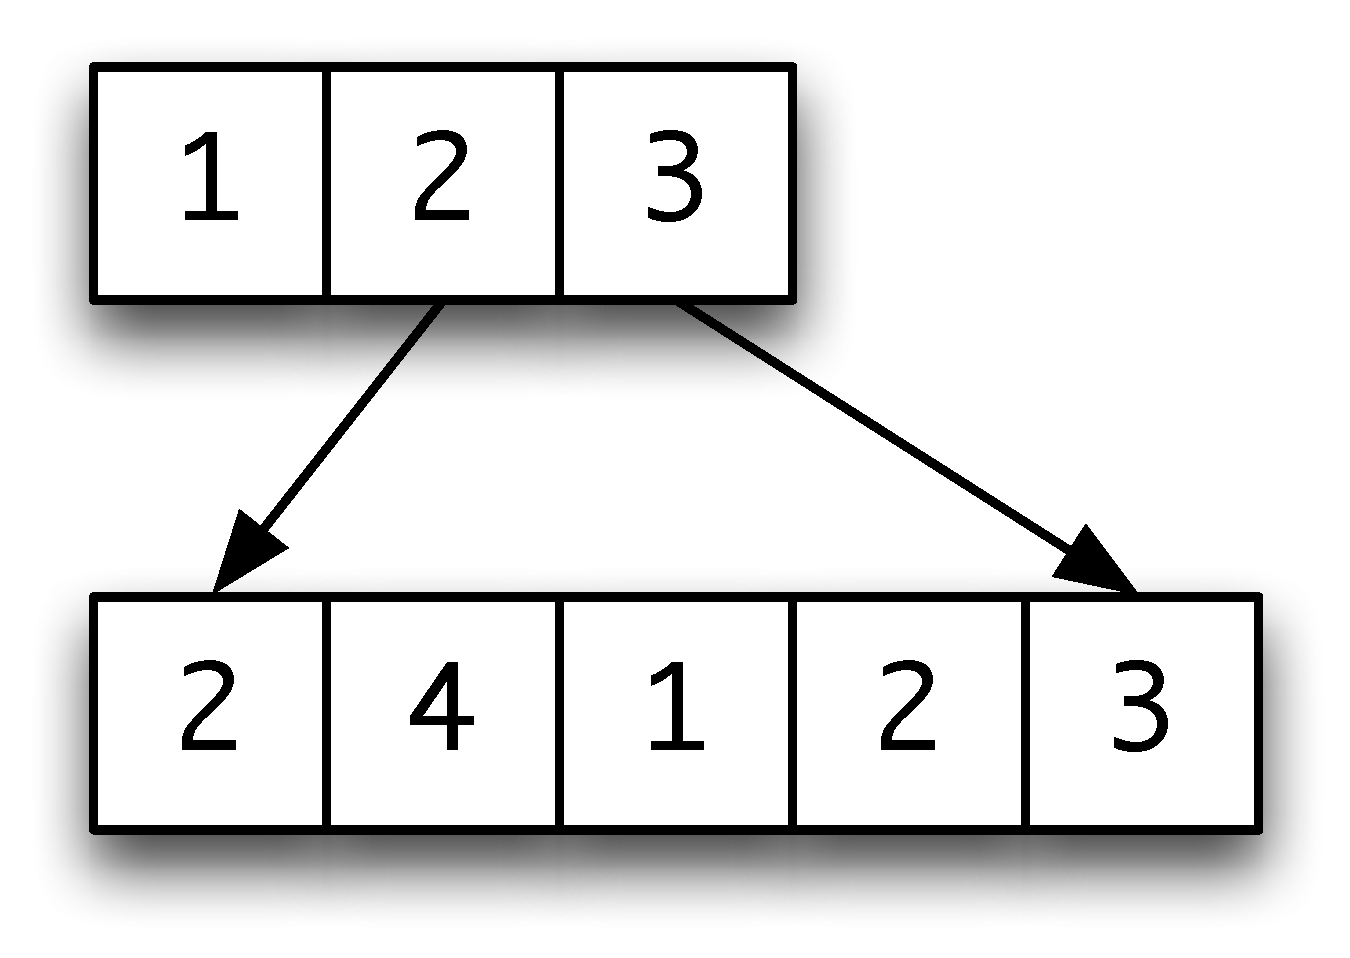
\includegraphics[width=1.7in]{Pictures/Greedy.pdf}
\end{center}
which is {\em not\/} optimal: the subsequence \texttt{[1,2,3]} has been missed,
since we make the choice of \texttt{2} the first element,  it is the first
point of agreement. This local choice is not part of an optimal global
solution, but the algorithm gives reasonable performance. 

In many situations, where local choices are always part of a global
solution, a greedy solution will work. Examples we have seen thus far include
\begin{titemize}
\item the line-splitting algorithm we gave in Chapter \ref{defFunLists} is optimal
in minimizing the sum of the inter-word spaces when the
lines are justified;
\index{text processing}
\item the Huffman codes described in Chapter \ref{codes} are optimal in the
sense of giving the shortest possible codings of files. We did not search all
possible sets of codes in giving the Huffman code, rather we built it up from
locally sensible choices. 
\index{Huffman codes}
\end{titemize}

\begin{exercises}

\item
Give an implementation of the greedy solution to the maximal common
subsequence problem, and show that it behaves as explained above on the
lists \texttt{[1,2,3]} and \texttt{[2,4,1,2,3]} above.

\item
Can you give an improvement of the maximal common subsequence solution along
the lines of \texttt{fibP}, returning a complex (finite) data structure as the
result of a function call, rather than simply one value?

\item
Finding the `edit distance' between two strings was first discussed in
Section  \ref{algDesign} where we gave a dynamic programming solution to the
problem. Show how you can give an efficient implementation of this
algorithm using the techniques of this section, and also how you give a greedy
solution to the problem. How do the two solutions compare? 

\item
Based on the examples of this section, provide a program which gives the
difference between two files, matching the corresponding lines  and giving the
output in a suitable form, such as a list of the pairs of matching line
numbers  or a form copied from the Unix \texttt{diff} program.
\end{exercises}

\begin{summary}
In this chapter we have examined the efficiency of lazy functional
programs. We saw that we are able to analyse the time
complexity of many of our more straightforward
functions without too much difficulty. To analyse
the space behaviour is more difficult, but we have shown how the space
consumption of lazy programs can be estimated from our calculations.

The introduction of \texttt{foldl} brings the space issue into focus, and the
distinction we made between strict and lazy functions allows us to
analyse the different behaviour of the two folds.

We concluded the discussion with an application of lazy infinite lists to 
memoizing results for reuse; the transition from naive to
efficient was done in a systematic way, which can be carried over to other
application areas. 

This chapter has provided an introduction to the study of functional
program behaviour; much more information -- particularly about
functional data structures -- can be found in \citeN{okasakiBook}.
\end{summary}

 
\index{behaviour|)}
\index{memoization|)}




%\end{document}

%\documentclass{book}\usepackage{sjtfonts}\usepackage{includegraphics}\usepackage{alltt}\usepackage{latexsym}
%\usepackage{array}
%\begin{document}\input{defs0}%		miradefs.tex 		    June 1994

% opening and closing a quoted Miranda section

\newcommand{\mira}{\noindent\hrulefill\nopagebreak\so}
\newcommand{\arim}{\nopagebreak\st\hrulefill\\}

% backslash in the Miranda environment
% Only feasible approach is to use \verb+\+
% in line!

%\newcommand{\bs}{$\mi\backslash\!\!$}
%\newcommand{\lbs}{\mbox{\verb+\+}}

% ignoring part of the input

\newcommand{\ignore}[1]{}

% a blank line in a Miranda section

\newcommand{\bl}{\mbox{\ }}

% Signalling a diffculty.

\definecolor{light-gray}{gray}{0.95}

\newcommand{\beware}[2]
 {\medskip\noindent\colorbox{light-gray}{\parbox{\textwidth}
 {\mbox{\large\textbf{#1}} \medskip\noindent\\ #2}\medskip\noindent}}

% Subscripting in Miranda text
\newcommand{\subscr}[2]{\mbox{${\mbox{\texttt{#1}}}_{\mbox{\texttt{#2}}}$}}

%\newcommand{\subscr}[2]{\mbox{${\mbox{\mi #1}}_{\mbox{\smtt #2}}$}}
\newcommand{\aone}{\subscr{a}{1}}
\newcommand{\atwo}{\subscr{a}{2}}
\newcommand{\ak}{\subscr{a}{k}}

\newcommand{\aoneone}{\subscr{a}{1,1}}

\newcommand{\eone}{\subscr{e}{1}}
\newcommand{\etwo}{\subscr{e}{2}}
\newcommand{\ei}{\subscr{e}{i}}
\newcommand{\er}{\subscr{e}{r}}

\newcommand{\fone}{\subscr{f}{1}}
\newcommand{\fl}{\subscr{f}{l}}

\newcommand{\gone}{\subscr{g}{1}}
\newcommand{\gtwo}{\subscr{g}{2}}
\newcommand{\gi}{\subscr{g}{i}}
\newcommand{\gr}{\subscr{g}{r}}

\newcommand{\hone}{\subscr{h}{1}}
\newcommand{\hl}{\subscr{h}{l}}

\newcommand{\pone}{\subscr{p}{1}}
\newcommand{\ptwo}{\subscr{p}{2}}
\newcommand{\pk}{\subscr{p}{k}}

\newcommand{\qone}{\subscr{q}{1}}
\newcommand{\qtwo}{\subscr{q}{2}}
\newcommand{\qk}{\subscr{q}{k}}

\newcommand{\rone}{\subscr{r}{1}}
\newcommand{\rtwo}{\subscr{r}{2}}

\newcommand{\tone}{\subscr{t}{1}}
\newcommand{\ttwo}{\subscr{t}{2}}
\newcommand{\tn}{\subscr{t}{n}}

\newcommand{\vone}{\subscr{v}{1}}
\newcommand{\vtwo}{\subscr{v}{2}}
\newcommand{\vn}{\subscr{v}{n}}

% for regular expressions

\newcommand{\stone}{\subscr{st}{1}}
\newcommand{\sttwo}{\subscr{st}{2}}
\newcommand{\stn}{\subscr{st}{n}}
\newcommand{\rthree}{\subscr{r}{3}}

\newcommand{\eps}{$\varepsilon$}
\newcommand{\trans}[1]{\stackrel{\mbox{\tt #1}}{\longrightarrow}}



% superscript in Miranda text

\newcommand{\superscr}[2]{\mbox{${\mbox{\mi #1}}^{\mbox{\smtt #2}}$}}

% Not equals in Miranda text

\newcommand{\noteq}{\makebox[0pt][l]{=}/}
\newcommand{\overslash}{\makebox[0pt][l]{/}}

% Definitions in complexity chapter

\newfont{\oldSym}{cmsy10}
\newcommand{\Th}{\boldmath$\oldSym\Theta$}
\newcommand{\pow}[1]{\^{}#1}
\newcommand{\leqq}{$\leq$}
\newcommand{\geqq}{$\geq$}
\newcommand{\lll}{$\ll$}
\newcommand{\eqq}{$\equiv$}
\newcommand{\ltwo}{\subscr{log}{2}}

% Indexing

\newcommand{\minx}[1]{\index{#1@{\ttfamily{}#1}}}
\setcounter{chapter}{19}\setcounter{page}{415}

%\minitocoptionfalse
\chapter{Conclusion}
\chapstart
\label{conclusion}

This book has covered the basics of functional programming
in the lazy language Haskell. It has shown how to craft programs, both by giving 
extensive examples as each new aspect of the language was introduced, and also by giving 
a series of larger case studies that run through the book. 

\section*{The power of functional programming}\index{functional programming!advantages of}
A functional programmer models the real world at a high level of
abstraction, concentrating on what relationships there are between
values, embodied in function definitions. This contrasts with a 
lower-level view  in which the details of how items are related predominate.
For instance, in Haskell lists are simply values, whereas in C or C++ they
become data structures built from pointers, and even in Java or C\# it is
difficult to present a suitably abstract model of lists.
This higher-level approach has a number of consequences, which have come out in the course
of the book.
\begin{itemize}

\item Higher-order functions and polymorphism combine to support the
construction of general-purpose libraries of functions, such as the list
functions in the Haskell standard prelude and library. The \texttt{map}
function, for instance,
\begin{alltt}
map :: (a -> b) -> [a] -> [b]
\end{alltt}
embodies the `pattern' of applying the same transformation to every
element in a list, which will be \textbf{reused} in a host of applications of
lists.
\itempar
Also supporting reuse through \textbf{overloading} are type classes, used for
instance in giving the function
\begin{alltt}
elem :: Eq a => a -> [a] -> Bool
\end{alltt}
which tests for membership of a list using the overloaded equality
function.

\item The definitions of functions are equations which express
properties of the functions defined. We can also express other properties of functions in a similar way. For example, we can relate 
\texttt{map} and
function composition, `\texttt{.}', by saying that  for all functions \texttt{f} and \texttt{g},
\begin{alltt}
map (f . g) ==  map f . map g
\end{alltt}
We can get \emph{strong evidence} that this property holds by testing it for randomly generated values of \texttt{f} and \texttt{g} using QuickCheck. 

\noindent
If we want to do some more work, we can \emph{prove} this property from the definitions of \texttt{map} and composition. 
Proof provides a user with assurance about how a program behaves on all arguments,
in contrast to testing which can only give direct information about its
behaviour on a (hopefully) representative selection of inputs.

\item Data structures can be introduced in a directly recursive manner,
giving trees, queues and so forth without having to look at their
representations. Algorithms are written at the same level as they would
be described informally, in contrast with more traditional approaches
which make the representation very clear.

\item Pulling all this together, we can use these and other facilities of Haskell to build implementations of domain-specific languages (DSLs) embedded in Haskell. These DSLs allow users to express problems and models in a language appropriate to the domain, but at the same time to use all the power of Haskell when necessary.

\end{itemize} 
A text like this can only provide an introduction to a subject as rich
and developed as functional programming; the rest of this concluding
chapter discusses other aspects of the subject, as well as giving pointers to 
other sources on the Web and in books and articles.

\section*{Further Haskell}
\index{Haskell!further features}

The purpose of this text is to introduce functional programming ideas using the
Haskell language. It covers the important aspects of the language, but does not
aim to be complete. Among the topics omitted are data types with labelled fields, which resemble
records or structures in other languages; strictness annotations, 
which are used to make data type constructors strict in some or all of their arguments; 
details of the \texttt{Read} class and the numeric types and classes. 

Further information about all these
can be found in the Haskell language report  \cite{haskell2010}, and the
`Gentle Introduction' of \cite{gentle98} also contains useful
information about some of them, as well as providing an
overview of the language for an experienced functional programmer. Both
of these, as well as many other Haskell resources, can be found at the
Haskell home page, \texttt{http://www.haskell.org/}.

Where can you go to find out what to do next in Haskell? Again the \texttt{haskell.org} site has many links, but three specific things you might like to look at are 
\begin{itemize}\index{Haskell!what to read next}
\item
\emph{Real World Haskell} \cite{realWorldHaskell} which is available in print and also online.  It starts from the beginning, but goes at a faster pace than we did here, and so covers a number of practical aspects of Haskell which we weren't able to do, such as the foreign function interface. So, it's the perfect follow-on read.
\item
\emph{Learn You a Haskell for Great Good!} \cite{learnYou} is a website and soon to be a printed book which introduces Haskell for those who are familiar with imperative programming. It's written in a very approachable style, and complements what we have covered here, as well as going into some topics -- like monads and zippers -- in much more detail.
\item
\emph{Pearls of Functional Algorithm Design} \cite{BirdPearls} this delightful book looks at a series of 30 problems, and solves them using the \emph{design by calculation} approach, which is ideally suited to writing functional programs in Haskell.
\end{itemize}
The text has discussed many of the most important functions in the
standard prelude but on the whole has avoided discussing the contents
of the libraries in detail. As we explained in Chapter \ref{progLists}, they are documented in Haddock, and this documentation is available online for type- and name-based search in Hoogle. Moreover, the packages in Hackage are themselves documented and have information available in Hayoo.

\subsection*{The future of Haskell}
\index{Haskell!prospects}

Haskell was first defined in 1987, and has been modified and extended a number of times
since then. This text is written in Haskell 2010,\index{Haskell 2010} which is meant to
provide a stable base system consisting of tried and tested features.

The progress of research in functional programming makes it clear that a
language like Haskell will not stand still, and Haskell is now undergoing regular language standard updates. These are set to incorporate features which have become \emph{de facto} parts of the language through their implementation in GHC, as well as more advanced features, particularly in the type system.
The Haskell home page
can be relied upon to contain up-to-date information on the status of Haskell.

\begin{figure}[t]
\begin{center}
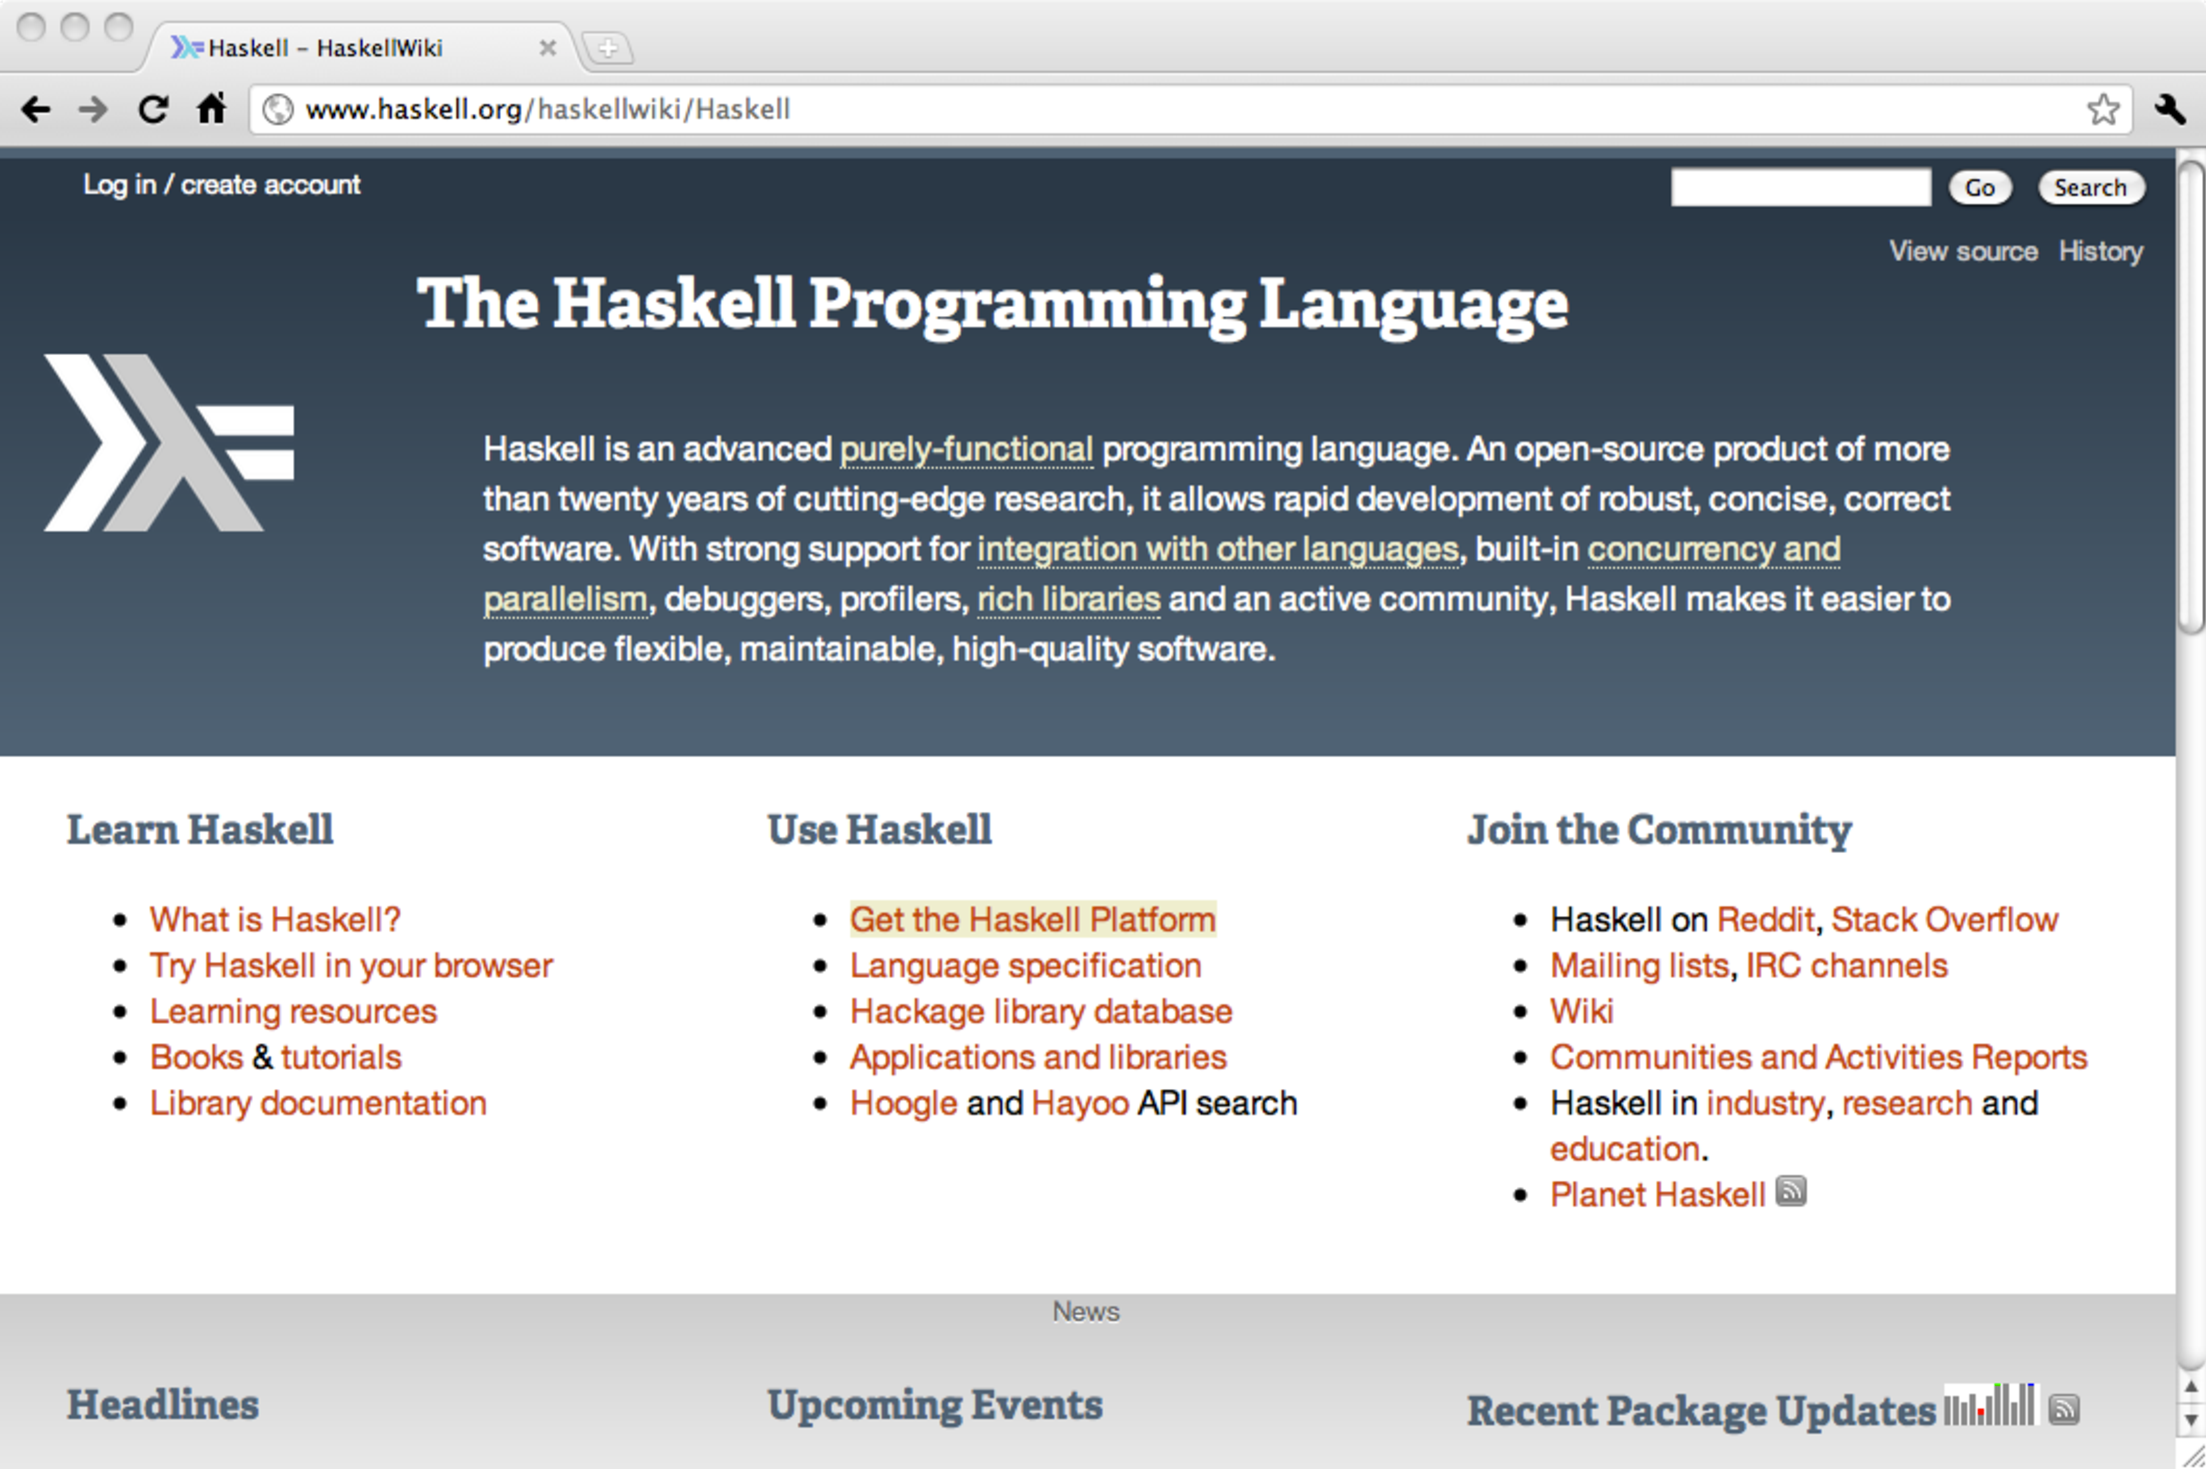
\includegraphics[width=5in]{Pictures/HaskellDotOrg.pdf}
\end{center}
\caption{The Haskell home page, \texttt{www.haskell.org}}
\label{HaskellDotOrg}
\end{figure}

\section*{Haskell on the web}
\index{Web site!sites with further information}

There are now many resources on Haskell and functional programming to be
found on the wbe. This text itself has a home page at
\begin{alltt}
www.haskellcraft.com
\end{alltt}
which lists all the links given here.
The Haskell home page, Figure \ref{HaskellDotOrg}, is at
\begin{alltt}
http://www.haskell.org/
\end{alltt}
and that should be your first stop for everything to do with Haskell. As you can see from the figure, the home page has links to learning resources, to documentation about libraries and packages, and to the wider Haskell community. 

The Haskell community includes online forums (IRC, mailing lists), news (Reddit), blogging (Planet Haskell) and help (Stack Overflow). The Haskell Communities and Activities reports provide a biannual snapshot of what's going on with Haskell: the most recent edition is 77 (two-column, A4) pages long, and contains a wealth of detail on who is doing what with Haskell. Subscribers to Planet Haskell or the mailing lists also receive Haskell Weekly News, which summarises Haskell-related software releases, blog entries and other news.

The Haskell language was named in honour of Haskell Brooks Curry. A
short biography and photograph of Curry can be found at\index{Curry,
Haskell B.!biography}
\begin{alltt}
http://www-history.mcs.st-and.ac.uk/Biographies/Curry.html
\end{alltt}

\section*{Other functional programming languages}\index{functional programming!other languages}

Haskell is a lazy, strongly typed functional programming language; 
another is Miranda \cite{mira,miraCraft}.\index{Miranda} In
this text laziness is only examined explicitly in Chapter \ref{lazy},
and up to that point it looks at aspects of functional programming which
are broadly shared with Standard ML\index{Standard ML} \shortcite{defsml2e,mlCritique}, the
best known and most widely used strict and strongly typed functional language, for which
\citeN{workingml2e} provides an introduction. The latest member of the ML family of languages, is F\# \cite{Fsharp}, which is distributed by Microsoft as a part of Visual Studio 2010. Since is possible to model
lazy evaluation within a strict language, and Haskell provides
facilities to make evaluation strict, the Haskell and ML schools of programming are very close
indeed.

A different style of functional programming, `point-free programming', eschews variables as much
as possible: this was introduced in \citeN{backus}. \citeN{AoP} is a text that
emphasizes the benefits of this style in supporting program
transformation and also advocates a `relational' style of programming
which extends the functional.

LISP is the oldest established functional language, but it differs from
Haskell and SML in not being strongly typed. An excellent tutorial
introduction to programming in the Scheme\index{Scheme} dialect of LISP is given in 
\citeN{strAndInterp}. \emph{Land of Lisp} \cite{LandOfLisp} is a book, website and music video\footnote{\ldots simple but refined, guaranteed to blow your mind \ldots} introducing Lisp by developing a series of games.
 
Erlang is a concurrent, fault-tolerant, distributed language, based on a functional programming core. Erlang \cite{progErlang,erlangProg} was developed within Ericsson, and as well as its use in telecoms applications, has applications in the financial sector, and to high-availability distributed systems in general. 

Two surveys of applications of functional programming languages in
large-scale projects are \citeN{applicsFP} and \citeN{stateArtFP}, and
there is also up-to-date information about this at the Haskell home page.

Over the last two decades, powerful techniques of implementation of especially
lazy functional languages have been developed. The twin texts
\cite{pj,pj-lester} describe the foundations of these in lucid detail.

\section*{Where is functional programming going?}\index{functional programming!future direction of}

The material in this text is an introduction to modern functional
programming in a typed, lazy, language. As the field develops, new
techniques and approaches are continually being developed; a good place
to start in learning about these is by looking at the proceedings of a series of summer
schools in Advanced Functional Programming
\cite{advancedFP,advancedFP2,advancedFP3,advancedFP4,advancedFP5,advancedFP6}. 

Research in functional programming is reported in the {\em Journal
of Functional Programming}
\begin{alltt}
http://journals.cambridge.org/jfp
\end{alltt} 
and at the annual
International Conference in Functional Programming, 
\begin{alltt}
http://www.icfpconference.org/
\end{alltt} 
Each year there is a one-day symposium devoted to research in Haskell, 
\begin{alltt}
www.haskell.org/haskell-symposium/
\end{alltt}
and the proceedings of this symposium (formerly workshop) will give you a view of the direction in which Haskell is going. 
The symposium is co-located with ICFP, as is the meeting of CUFP,
\texttt{cufp.org},
which represents Commercial Users of Functional Programming.

To see the ways in which functional
languages are being used in education, the proceedings of a meeting on
Functional Languages in Education appear in \citeN{fple95}, and these
have been followed up with a series of occasional workshops co-located with ICFP.

It is difficult to predict future directions in a field like computing. In the previous edition of this book (written 1998--9) I predicted three things:
\begin{itemize}
\item functional languages will come to be used as parts of larger systems;
\item type systems for languages like Haskell will become more powerful and esoteric, and
\item tool support, for instance giving feedback on the behaviour of lazy programs, will come to maturity.
\end{itemize}
Not a bad set of predictions. The first is certainly true, with Haskell inter-operating effectively with a range of other languages through its foreign function interface. GCH continues to be a laboratory for type system research, with recent advances in type-level programming taking it ever closer to dependently-typed languages such as Agda,\index{Agda}\index{type!dependent types}
\begin{alltt}
http://wiki.portal.chalmers.se/agda/
\end{alltt}
Tool support for Haskell has also come of age, with many tools integrated into GHC, and it becoming easier for others to integrate their work through the definition of an API for the internals of GHC. What I had not predicted was the growth in the Haskell developer community: fuelled particularly by Hackage and Cabal, making it easy to share and to work collaboratively, there are now close to three thousand projects on Hackage, giving the developer community a critical mass which was entirely lacking a decade ago.\footnote{It was also a surprise that Microsoft started to deploy a functional language as a part of their main language suite in Visual Studio: a friend mailed me and said that his first thought it was an `April fool' message, even though it came in June!} 

What of the next few years? The big challenge for systems developers is the rise of multicore chips: chips with thousands of processors are on the roadmap, and so the question arises of how best to program them, or indeed how to program them at all! Functional languages, because of their lack of side-effects, and clean models for concurrency, make them ideal candidates for the next generation of general purpose languages for multicore. The next few years will be fascinating, and of course, unpredictable, but it will be a surprise if functional languages are not playing a much more important role in robust software development in ten years time, with Haskell central to this achievement.


%\end{document}

\appendix
%\documentclass{book}\usepackage{sjtfonts}\usepackage{includegraphics}\usepackage{alltt}\usepackage{latexsym}
%\usepackage{array}
%\begin{document}\input{defs0}%		miradefs.tex 		    June 1994

% opening and closing a quoted Miranda section

\newcommand{\mira}{\noindent\hrulefill\nopagebreak\so}
\newcommand{\arim}{\nopagebreak\st\hrulefill\\}

% backslash in the Miranda environment
% Only feasible approach is to use \verb+\+
% in line!

%\newcommand{\bs}{$\mi\backslash\!\!$}
%\newcommand{\lbs}{\mbox{\verb+\+}}

% ignoring part of the input

\newcommand{\ignore}[1]{}

% a blank line in a Miranda section

\newcommand{\bl}{\mbox{\ }}

% Signalling a diffculty.

\definecolor{light-gray}{gray}{0.95}

\newcommand{\beware}[2]
 {\medskip\noindent\colorbox{light-gray}{\parbox{\textwidth}
 {\mbox{\large\textbf{#1}} \medskip\noindent\\ #2}\medskip\noindent}}

% Subscripting in Miranda text
\newcommand{\subscr}[2]{\mbox{${\mbox{\texttt{#1}}}_{\mbox{\texttt{#2}}}$}}

%\newcommand{\subscr}[2]{\mbox{${\mbox{\mi #1}}_{\mbox{\smtt #2}}$}}
\newcommand{\aone}{\subscr{a}{1}}
\newcommand{\atwo}{\subscr{a}{2}}
\newcommand{\ak}{\subscr{a}{k}}

\newcommand{\aoneone}{\subscr{a}{1,1}}

\newcommand{\eone}{\subscr{e}{1}}
\newcommand{\etwo}{\subscr{e}{2}}
\newcommand{\ei}{\subscr{e}{i}}
\newcommand{\er}{\subscr{e}{r}}

\newcommand{\fone}{\subscr{f}{1}}
\newcommand{\fl}{\subscr{f}{l}}

\newcommand{\gone}{\subscr{g}{1}}
\newcommand{\gtwo}{\subscr{g}{2}}
\newcommand{\gi}{\subscr{g}{i}}
\newcommand{\gr}{\subscr{g}{r}}

\newcommand{\hone}{\subscr{h}{1}}
\newcommand{\hl}{\subscr{h}{l}}

\newcommand{\pone}{\subscr{p}{1}}
\newcommand{\ptwo}{\subscr{p}{2}}
\newcommand{\pk}{\subscr{p}{k}}

\newcommand{\qone}{\subscr{q}{1}}
\newcommand{\qtwo}{\subscr{q}{2}}
\newcommand{\qk}{\subscr{q}{k}}

\newcommand{\rone}{\subscr{r}{1}}
\newcommand{\rtwo}{\subscr{r}{2}}

\newcommand{\tone}{\subscr{t}{1}}
\newcommand{\ttwo}{\subscr{t}{2}}
\newcommand{\tn}{\subscr{t}{n}}

\newcommand{\vone}{\subscr{v}{1}}
\newcommand{\vtwo}{\subscr{v}{2}}
\newcommand{\vn}{\subscr{v}{n}}

% for regular expressions

\newcommand{\stone}{\subscr{st}{1}}
\newcommand{\sttwo}{\subscr{st}{2}}
\newcommand{\stn}{\subscr{st}{n}}
\newcommand{\rthree}{\subscr{r}{3}}

\newcommand{\eps}{$\varepsilon$}
\newcommand{\trans}[1]{\stackrel{\mbox{\tt #1}}{\longrightarrow}}



% superscript in Miranda text

\newcommand{\superscr}[2]{\mbox{${\mbox{\mi #1}}^{\mbox{\smtt #2}}$}}

% Not equals in Miranda text

\newcommand{\noteq}{\makebox[0pt][l]{=}/}
\newcommand{\overslash}{\makebox[0pt][l]{/}}

% Definitions in complexity chapter

\newfont{\oldSym}{cmsy10}
\newcommand{\Th}{\boldmath$\oldSym\Theta$}
\newcommand{\pow}[1]{\^{}#1}
\newcommand{\leqq}{$\leq$}
\newcommand{\geqq}{$\geq$}
\newcommand{\lll}{$\ll$}
\newcommand{\eqq}{$\equiv$}
\newcommand{\ltwo}{\subscr{log}{2}}

% Indexing

\newcommand{\minx}[1]{\index{#1@{\ttfamily{}#1}}}
\setcounter{chapter}{19}\setcounter{page}{415}
\addtocontents{toc}{\contentsline {chapter}{Appendices}{}}

%\minitocoptionfalse

\chapter{Functional, imperative and OO programming}
\label{vs}
\index{imperative programming|(}

In this appendix we compare programming in Haskell to more traditional
notions in imperative languages like Pascal and C and object-oriented
(OO)
languages such as C\#, C++ and Java.

\section*{Values and states}
\index{value}\index{state}

Consider the example of finding the sum of squares
of natural numbers up to a particular number. 
A functional program describes the values that are to be calculated, directly. 
\begin{alltt}
sumSquares :: Int -> Int
sumSquares 0 = 0
sumSquares n = n*n + sumSquares (n-1)
\end{alltt}
These equations state what the sum of squares is for a natural number
argument. In the first case it
is a direct description; in the second it states that the sum to non-zero
\texttt{n} is
got by finding the sum to \texttt{n-1} and adding the square of \texttt{n}.

A typical imperative program might solve the problem thus
\begin{alltt}
s = 0 ;
i = 0 ;
while i<n do 
  begin
    i = i+1 ;
    s = i*i + s ;
  end 
\end{alltt}
The sum is the final value of the variable \texttt{s}, which is changed repeatedly
during program execution, as is the `count' variable, \texttt{i}.
The effect of the program can only be seen by following the  sequence of changes
made to these variables by the commands in the program, while  the
functional program can be read as a series of equations defining the sum of squares. This meaning is \textbf{explicit} in the functional program, whereas the imperative program has an overall effect which is not obvious from the program itself. 


The link between these two approaches is given by a tail-recursive solution to the problem in Haskell:
\begin{alltt}
sumSquares n = ssAcc 0 0 n

ssAcc i s n
  | i<n       = ssAcc (i+1) ((i+1)^2+s) n
  | otherwise = s
\end{alltt}
Here the three argument positions play the role of three variables -- \texttt{i}, \texttt{s} and \texttt{n} -- whose values are changed on each call to the loop.

A more striking algorithm still is one which is completely explicit:
`to find the sum of squares, build the list of numbers \texttt{1} to 
\texttt{n}, square each of them, and sum the result'.
This program, which uses neither complex control flow, as does the imperative
example, nor recursion as seen in the function \texttt{sumSquares}, can be written
in a functional style, thus:
\begin{alltt}
newSumSq :: Int -> Int
newSumSq n = sum (map square [1 ..\ n])
\end{alltt}
where \texttt{square x = x*x}, the operation \texttt{map}
applies its first argument to every member of a list, and \texttt{sum} finds the
sum of a list of numbers. More examples of this sort of \textbf{data-directed}
programming\index{data-directed programming}
can be seen in the body of the text.

\section*{Functions and variables}

An important difference between the two styles
is what is meant by some of the terminology. Both `function' and `variable'
have different interpretations.

\index{function}
As was explained earlier, a function in a functional program is simply
something which returns a value which depends upon some inputs. In 
imperative and object-oriented languages like Pascal, C, C++ and Java a 
function is rather different. It will
return a value depending upon its arguments, but in general it will also 
change the
values of variables. Rather than being a pure function it is really
a procedure which returns a value when it terminates. 

\index{variable}
In a functional program a variable stands for an \textbf{arbitrary} or \textbf{
unknown} value. Every occurrence of a variable in an equation is interpreted
in the same way. They are  just like variables in logical formulas,
or the mathematical variables familiar from
equations like
\begin{alltt}
\superscr{a}{2} - \superscr{b}{2} = (a-b)(a+b)
\end{alltt}
In any particular case, the value of all three occurrences of \texttt{a} will be
the same. In exactly the same way, in
\so
sumSquares n = n*n + sumSquares (n-1)
\st
all occurrences of \texttt{n} will be interpreted by the same value. For example
\so
sumSquares 7 = 7*7 + sumSquares (7-1)
\st
The crucial motto is `variables in functional programs {\em do not vary}'.

On the other hand, the value of a variable in an imperative
program changes throughout its lifetime. In the sum of squares program above,
the variable \texttt{s} will take the values \texttt{0,1,5,\ldots} successively.
Variables in imperative programs {\em do\/} vary over time, on the other hand.

\section*{Program verification}
\index{proof}
\vspace{-6pt}

Probably the most important difference between functional and imperative
programs is logical. 
As well as being a program, a functional definition is a logical equation
describing a \textbf{property} of the function. Functional
programs are \textbf{self-describing}, as it were. Using the definitions, other
properties of the functions can be deduced. 

To take a simple example, for all
\texttt{n>0}, it is the case that 
\begin{alltt}
sumSquares n > 0
\end{alltt}
To start with,
\begin{alltt}
sumSquares 1 
= 1*1 + sumSquares 0
= 1*1 + 0
= 1
\end{alltt}
which is greater than 0. In general, for \texttt{n} greater than zero,
\begin{alltt}
sumSquares n = n*n + sumSquares (n-1)
\end{alltt}
Now, \texttt{n*n} is positive, and if \texttt{sumSquares (n-1)} is positive,
their sum, \texttt{sumSquares n}, must be. This proof can be formalized using
\textbf{mathematical induction}\index{mathematical induction}. The body
of the text contains numerous examples of proofs by induction over the
structure of data structures like lists and trees, as well as over
numbers.

Program verification is possible for imperative programs as well, but
imperative programs are not self-describing in the way functional ones are.
To describe the effect of an imperative program, like the `sum of squares'
program above, we need to add to the program logical formulas or assertions
which describe the state of the program at various points in its execution.
These methods are both more indirect and more difficult, and verification
seems very difficult indeed for `real' languages like Pascal and 
C. Another aspect of program verification is \textbf{program transformation} in
which programs are transformed to other programs which have the same effect but
better performance, for example. Again, this is difficult for
traditional imperative languages.


\section*{Records and tuples}
\index{tuples}\index{records}
\vspace{-6pt}

In Chapter \ref{tupleList} the tuple types of Haskell are introduced. In
particular we saw the definition
\begin{alltt}
type Person = (String,String,Int)
\end{alltt}
This compares with a Pascal declaration of a record
\begin{alltt}
type Person = record 
  name  : String;
  phone : String;
  age   : Integer
end;
\end{alltt} 
which has three fields which have to be named. In Haskell the fields of a
tuple can be accessed by pattern matching, but it is possible to define
functions called \textbf{selectors} which behave in a similar way, if
required:  
\begin{alltt}
name  :: Person -> String
name (n,p,a) = n
\end{alltt}
and so on. If \texttt{per ::\ Person} then \texttt{name per ::\ String}, similarly
to  \texttt{r.name} being a string variable if \texttt{r} is a variable of type 
\texttt{Person} in Pascal.

We could instead use an algebraic type to represent a person:
\begin{alltt}
data Person = Person {name::String, phone::String, age::Integer}
              deriving (Show,Eq)
\end{alltt}
In an object-oriented language like Java or C\# this type would be represented by an \emph{object} wit three attributes, one for each of the name, phone and age.  The methods modifying these values would also be part of the definition of the object.

To implement the analogue of an algebraic data type with more than one constructor in Java it is necessary to work rather harder. The type itself is modelled as a class with abstract methods, implemented in a number of sub-classes, one per constructor. Each sub-class contains the attributes for a particular constructor, together with the implementation of the methods over that sub-class. This approach works well for methods that work over one member of a class, but is more problematic for binary methods, and in particular for equality.




\section*{Lists and pointers}
\index{pointer}
\vspace{-5pt}

Haskell contains the type of lists built in, and other recursive types such as
trees can be defined directly. We can think of the type of linked lists given
by pointers in Pascal as an \textbf{implementation} of lists, since in Haskell
it is not necessary to think of pointer values, or of storage allocation (
\texttt{new} and \texttt{dispose}) as it is in Pascal. Indeed, we can think of Haskell
programs as \textbf{designs} for Pascal list programs.
If we define
\index{lists!as Pascal type}
\begin{alltt}
type list = \^{}node;
type node = record
   head : value;
   tail : list
end;
\end{alltt}
then we have the following correspondence, where the Haskell \texttt{head} and
\texttt{tail} functions give the head and tail of a list.
\begin{alltt}
            []                        nil
            head ys                   ys\^{}.head 
            tail ys                   ys\^{}.tail 
            (x:xs)                    cons(x,xs) 
\end{alltt}
The function \texttt{cons} in Pascal has the definition
\begin{alltt}
function cons(y:value;ys:list):list;
  var xs:list;
  begin
    new(xs);
    xs\^{}.head := y;
    xs\^{}.tail := ys;
    cons := xs
  end;
\end{alltt}
Functions such as 
\begin{alltt}
sumList []     = 0 
sumList (x:xs) = x + sumList xs 
\end{alltt}
can then be transferred to Pascal in a
straightforward way.
\begin{alltt}
function sumList(xs:list):integer;
  begin
    if xs=nil 
      then sumList := 0
      else sumList := xs\^{}.head + sumList(xs\^{}.tail)
  end;
\end{alltt}
A second example is 
\begin{alltt}
doubleAll []     = []
doubleAll (x:xs) = (2*x) : doubleAll xs
\end{alltt}
where
we use \texttt{cons} in the Pascal definition of the function
\begin{alltt}
function doubleAll(xs:list):list;
  begin
    if xs=nil 
      then doubleAll := nil
      else doubleAll := cons( 2*xs\^{}.head , doubleAll(xs\^{}.tail) )
  end;
\end{alltt}
If we define the functions
\begin{alltt}
function head(xs:list):value;     function tail(xs:list):list;
  begin                            begin
    head := xs\^{}.head                 tail := xs\^{}.tail
  end;                             end;
\end{alltt}
then the correspondence is even clearer:
\begin{alltt}
function doubleAll(xs:list):list;
  begin
    if xs=nil 
      then doubleAll := nil
      else doubleAll := cons( 2*head(xs) , doubleAll( tail(xs) ) )
  end;
\end{alltt}
This is strong evidence that a functional approach can be useful even if  we
are writing in an imperative language: the functional language can be the
high-level {\em design\/}\index{design}
language for the imperative implementation. Making
this separation can give us substantial help in finding imperative programs
-- we can think about the design and the lower level implementation {\em
separately}, which makes each problem smaller, simpler and therefore easier
to solve.
\vspace{-5pt}

\section*{Higher-order functions}
\index{higher-order function}
\vspace{-5pt}

Traditional imperative languages give little scope for higher-order
programming; Pascal, Java and C allow functions as arguments, so long as those
functions are not themselves higher-order, but has no facility for returning
functions as results. In C++ it is possible to return objects which
represent functions by overloading the function application operator!
This underlies the genericity hailed in the C++ Standard Template Library,
which requires advanced features of the language to implement functions
like \texttt{map} and \texttt{filter}.

Control structures like \texttt{if-then-else} bear some resemblance to
higher-order functions, as they take commands, \texttt{\subscr{c}{1}}, 
\texttt{\subscr{c}{2}} etc.\ into other commands, 
\begin{alltt}
if b then \subscr{c}{1} else \subscr{c}{2}\ \ \ \ \ \ while b do \subscr{c}{1}
\end{alltt}
just as \texttt{map} takes one function to another. Turning the analogy around,
we can think of higher-order functions in Haskell
as \textbf{control structures} which we
can define ourselves. This perhaps explains why we form libraries of
polymorphic functions: they are the control structures we use in programming
particular  sorts of system. Examples in the text include libraries for
building parsers (Section \ref{parsing}) and interactive I/O programs
(Chapter \ref{io}), as well as the built-in list-processing
functions.
\vspace{-2pt}

\section*{Polymorphism}
\index{polymorphism}
\vspace{-2pt}

Again, this aspect is poorly represented in many imperative languages; the
best we can do in \texttt{Pascal}, say, is to use a text editor to copy and
modify the list processing code from one type of lists for use with another.
Of course, we then run the risk that the different versions of the programs
are not modified in step, unless we are very careful to keep track of
modifications, and so on.


Polymorphism in Haskell is what is commonly known as
\textbf{generic} polymorphism: the same `generic' code works over a
whole collection of types. A simple example is the function which 
reverses the elements in a list.

Haskell classes support what is known as `ad
hoc' polymorphism, or in object-oriented terminology simply `polymorphism', 
in which different programs implement the same
operation over different types. An example of this is the \texttt{Eq}
class of types carrying an equality operation: the way in which equality
is checked is completely different at different types. Another way of
viewing classes is as \textbf{interfaces}\index{interface} which different types
can implement in different ways; in this way they resemble the
interfaces of object-oriented languages like Java.

As is argued in the text, polymorphism is one of the mechanisms which helps to
make programs {\em reusable\/} in Haskell; it remains to be seen whether this
will also be true of advanced imperative languages.
\vspace{-2pt}

\section*{Defining types and classes}
\vspace{-2pt}

The algebraic type mechanism of Haskell, explained in Chapter \ref{algTypes},
\index{algebraic type}
subsumes various traditional type definitions. Enumerated types are given by
algebraic types all of whose constructors are 0-ary (take no arguments);
variant records can be implemented as algebraic types with more then one
constructor, and \textbf{recursive} types usually implemented by means of
pointers become recursive algebraic types.

Just as we explained for lists, Haskell programs over trees and so on can be
seen as {\em designs\/} for programs in imperative languages manipulating the
pointer implementations of the types.

The abstract data types\index{abstract data type},
introduced in Chapter \ref{adt}, are very like the abstract
data types of \texttt{Modula-2} and so on; the design  methods we suggest for
use of abstract data types mirror
aspects of the \textbf{object-based} approach advocated for
modern imperative languages such as \texttt{Ada}. 

\index{classes}
The Haskell class system also has object-oriented aspects, as we saw in
Section \ref{algClasses}. It is important to note that Haskell classes are in
some ways quite different from the classes of, for instance, \texttt{C++}. In
Haskell classes are made up of types, which themselves have members; in 
\texttt{C++} a class is like a type, in that it contains objects. Because of this many
of the aspects of object-oriented design in \texttt{C++} are seen as issues of
type design in Haskell.
\vspace{-3pt}

\section*{List comprehensions}
\index{list comprehensions}
\vspace{-3pt}

List comprehensions provide a convenient notation for \textbf{iteration\/} along
lists: the analogue of a \texttt{for} loop, which can be used to run through the
indices of an array. For instance, to sum all pairs of elements of \texttt{xs} and
\texttt{ys}, we write
\begin{alltt}
[ a+b | a <- xs , b <- ys ]
\end{alltt}
The order of the iteration is for a value \texttt{a} from the list \texttt{xs} to be
fixed and then for \texttt{b} to run through the possible values from \texttt{ys};
this is then repeated with the next value from \texttt{xs}, until the list is
exhausted. Just the same happens for a \textbf{nested\/} \texttt{for} loop
\begin{alltt}
for i:=0 to xLen-1 do
  for j:=0 to yLen-1 do\hfill (twoFor)
    write( x[i]+y[j] ) 
\end{alltt}
where we fix a value for \texttt{i} while running through all values for 
\texttt{j}.

In the \texttt{for} loop, we have to run through the indices; a list generator
runs through the values directly. The indices of the list
\texttt{xs} are given by 
\begin{alltt}
[0 ..\ length xs - 1]
\end{alltt}
and so a Haskell analogue of 
\texttt{(twoFor)} can be written thus:
\begin{alltt}
[ xs!!i + ys!!j | i <- [0 ..\ length xs - 1] , 
                  j <- [0 ..\ length ys - 1] ]
\end{alltt}
if we so wish. 
\vspace{-3pt}

\section*{Lazy evaluation}
\index{lazy evaluation}
\vspace{-3pt}

Lazy evaluation and imperative languages do not mix well. In \texttt{Pascal},
for instance, we can write the function definition
\begin{alltt}
function succ(x : integer):integer;
begin
  y    := y+1;
  succ := x+1
end;
\end{alltt}
This function adds one to its argument, but also has the \textbf{side-effect\/}
of increasing \texttt{y} by one. If we evaluate \texttt{f(y,succ(z))} we cannot
predict the effect it will have.
\begin{titemize}
\item If \texttt{f} evaluates its second argument first, \texttt{y} will be
increased before being passed to \texttt{f}; 
\item on the other hand, if \texttt{f} needs its first argument first (and perhaps its second
argument not at all), the value passed to \texttt{f} will not be increased, even
if it is increased before the function call terminates.
\end{titemize}
In general, it will not be possible to predict the behaviour of even the
simplest programs. Since evaluating an expression can cause a change of the
state, the order of expression evaluation determines the overall effect of a
program, and so a lazy implementation can behave differently (in unforeseen
ways) from the norm.

\section*{State, infinite lists and monads}
\index{lists!infinite}\index{state}\index{monad}

Section \ref{infLists} introduced infinite lists, and one of the first
examples given there was an infinite list of random numbers. This list could
be supplied to a function requiring a supply of random numbers; because of lazy
evaluation, these numbers will only be generated on demand. 

If we were to implement this imperatively, we would probably keep in a
variable the last random number generated, and at each request for a
number we would update this store. We can see the infinite list as supplying
{\em all the values that the variable will take\/} as a single structure; we
therefore do not need to keep the state, and hence have an \textbf{abstraction\/} from the imperative view.

We have seen in Section \ref{monadFP} that there has been recent important
work on integrating side-effecting programs into a functional system by a
monadic approach.

\section*{Conclusion}

Clearly there are parallels between the functional and the imperative, as
well as clear differences. The functional view of a system is often
higher-level, and so even if we ultimately aim for an imperative solution, a
functional design  or \textbf{prototype\/} can be most useful.

We have seen that monads can be used to give an interface to 
imperative features within a functional framework. Many of the Haskell
implementations offer these facilities, and so give a method of uniting the
best features of two important programming paradigms without compromising the
purity of the language. Other languages,
including Standard ML \cite{defsml} and F\# \cite{Fsharp}, combine the functional and the imperative, but
these systems tend to lose their pure functional properties in the process.

It is interesting to see the influence of ideas from modern functional
programming languages in the design of Java extensions. One of the main
drawbacks of Java for a long time was that it lacked generic polymorphism. The current 
mechanism for generics in the Java standard owes its inspiration and much of its detail to Haskell polymorphism.


\index{imperative programming|)}

%\end{document}

%\documentclass{book}\usepackage{sjtfonts}\usepackage{includegraphics}\usepackage{alltt}\usepackage{latexsym}
%\usepackage{array}\usepackage{multicol}
%\begin{document}\input{defs0}%		miradefs.tex 		    June 1994

% opening and closing a quoted Miranda section

\newcommand{\mira}{\noindent\hrulefill\nopagebreak\so}
\newcommand{\arim}{\nopagebreak\st\hrulefill\\}

% backslash in the Miranda environment
% Only feasible approach is to use \verb+\+
% in line!

%\newcommand{\bs}{$\mi\backslash\!\!$}
%\newcommand{\lbs}{\mbox{\verb+\+}}

% ignoring part of the input

\newcommand{\ignore}[1]{}

% a blank line in a Miranda section

\newcommand{\bl}{\mbox{\ }}

% Signalling a diffculty.

\definecolor{light-gray}{gray}{0.95}

\newcommand{\beware}[2]
 {\medskip\noindent\colorbox{light-gray}{\parbox{\textwidth}
 {\mbox{\large\textbf{#1}} \medskip\noindent\\ #2}\medskip\noindent}}

% Subscripting in Miranda text
\newcommand{\subscr}[2]{\mbox{${\mbox{\texttt{#1}}}_{\mbox{\texttt{#2}}}$}}

%\newcommand{\subscr}[2]{\mbox{${\mbox{\mi #1}}_{\mbox{\smtt #2}}$}}
\newcommand{\aone}{\subscr{a}{1}}
\newcommand{\atwo}{\subscr{a}{2}}
\newcommand{\ak}{\subscr{a}{k}}

\newcommand{\aoneone}{\subscr{a}{1,1}}

\newcommand{\eone}{\subscr{e}{1}}
\newcommand{\etwo}{\subscr{e}{2}}
\newcommand{\ei}{\subscr{e}{i}}
\newcommand{\er}{\subscr{e}{r}}

\newcommand{\fone}{\subscr{f}{1}}
\newcommand{\fl}{\subscr{f}{l}}

\newcommand{\gone}{\subscr{g}{1}}
\newcommand{\gtwo}{\subscr{g}{2}}
\newcommand{\gi}{\subscr{g}{i}}
\newcommand{\gr}{\subscr{g}{r}}

\newcommand{\hone}{\subscr{h}{1}}
\newcommand{\hl}{\subscr{h}{l}}

\newcommand{\pone}{\subscr{p}{1}}
\newcommand{\ptwo}{\subscr{p}{2}}
\newcommand{\pk}{\subscr{p}{k}}

\newcommand{\qone}{\subscr{q}{1}}
\newcommand{\qtwo}{\subscr{q}{2}}
\newcommand{\qk}{\subscr{q}{k}}

\newcommand{\rone}{\subscr{r}{1}}
\newcommand{\rtwo}{\subscr{r}{2}}

\newcommand{\tone}{\subscr{t}{1}}
\newcommand{\ttwo}{\subscr{t}{2}}
\newcommand{\tn}{\subscr{t}{n}}

\newcommand{\vone}{\subscr{v}{1}}
\newcommand{\vtwo}{\subscr{v}{2}}
\newcommand{\vn}{\subscr{v}{n}}

% for regular expressions

\newcommand{\stone}{\subscr{st}{1}}
\newcommand{\sttwo}{\subscr{st}{2}}
\newcommand{\stn}{\subscr{st}{n}}
\newcommand{\rthree}{\subscr{r}{3}}

\newcommand{\eps}{$\varepsilon$}
\newcommand{\trans}[1]{\stackrel{\mbox{\tt #1}}{\longrightarrow}}



% superscript in Miranda text

\newcommand{\superscr}[2]{\mbox{${\mbox{\mi #1}}^{\mbox{\smtt #2}}$}}

% Not equals in Miranda text

\newcommand{\noteq}{\makebox[0pt][l]{=}/}
\newcommand{\overslash}{\makebox[0pt][l]{/}}

% Definitions in complexity chapter

\newfont{\oldSym}{cmsy10}
\newcommand{\Th}{\boldmath$\oldSym\Theta$}
\newcommand{\pow}[1]{\^{}#1}
\newcommand{\leqq}{$\leq$}
\newcommand{\geqq}{$\geq$}
\newcommand{\lll}{$\ll$}
\newcommand{\eqq}{$\equiv$}
\newcommand{\ltwo}{\subscr{log}{2}}

% Indexing

\newcommand{\minx}[1]{\index{#1@{\ttfamily{}#1}}}
\appendix


\newcommand{\gitem}[1]{\medskip\noindent{\bf #1\ \ \ }
                       %\raggedright
                       }

\newcommand{\upp}[1]{\ensuremath{{}^{\mbox{\footnotesize\texttt #1}}}}

%\minitocoptionfalse
\chapter{Glossary}

We include this glossary to give a quick reference to the most
widely used terminology in the book. Words appearing in \textbf{bold} in the
descriptions have their own entries. Further references and examples are
to be found by consulting the index.
\normalfont\normalsize
\hspace*{12pt} 


\begin{multicols}{2}

{\raggedright

\gitem{Abstract type}\index{abstract data type}
An abstract type definition consists of the type name, the \textbf{signature} of
the type, and the implementation equations for the names in the
signature.

\gitem{Algebraic type}\index{algebraic type}
An algebraic type definition states what are the \textbf{constructors} of the
type. For instance, the declaration
\begin{alltt}
data Tree = Leaf Int | 
            Node Tree Tree
\end{alltt}
says that the two constructors of the \texttt{Tree} type are
\texttt{Leaf} and \texttt{Node}, and that their types are, respectively,
\begin{alltt}
Leaf :: Int->Tree
Node :: Tree->Tree->Tree
\end{alltt}

\gitem{Application}\index{function application}
This means giving values to (some of) the arguments
of a function. If an \texttt{n}-argument function is given fewer than \texttt{n}
arguments, this is called a \textbf{partial application}.
Application is written using \textbf{juxtaposition}.

\gitem{Argument}\index{argument}
A \textbf{function} takes one or more arguments into an \textbf{output}. Arguments
are also known as \textbf{inputs} and \textbf{parameters}.

\gitem{Associativity}\index{associativity}
The way in which an expression involving two applications of an operator is
interpreted. If \texttt{x\#y\#z} is interpreted as \texttt{(x\#y)\#z} then
\texttt{\#} is left associative, if as \texttt{x\#(y\#z)} it is right associative;
if both bracketings give the same result then \texttt{\#} is called associative.

\gitem{Base types}\index{type!base}
The types of numbers, including
\texttt{Int} and \texttt{Float}, \textbf{Booleans}, \texttt{Bool}, and \textbf{characters},
\texttt{Char}.

\gitem{Binding power}\index{operator!binding power of}
The `stickiness' of an operator, expressed as an integer; the higher the
number the stickier the operator. For example, \texttt{2+3*4} is interpreted as
\texttt{2+(3*4)} as `\texttt{*}' has higher binding power -- binds more tightly 
-- than `\texttt{+}'.

\gitem{Booleans}\index{Booleans}
The type containing the two `truth values' \texttt{True} and \texttt{False}.

\gitem{Calculation}\index{calculation}
A calculation is a line-by-line \textbf{evaluation} of a Haskell \textbf{expression}
on paper. Calculations use the \textbf{definitions} which are contained in a
\textbf{script} as well as the built-in definitions.

\gitem{Cancellation}\index{type checking!rule of cancellation}
The rule for finding the type of a partial application.

\gitem{Character}\index{characters}
A single letter, such as \texttt{'s'} or \texttt{'\bs{t}'}, the tab character.
They form the \texttt{Char} type.

\gitem{Class}\index{classes}
A collection of types. A class is defined by specifying a \textbf{signature};
a type is made an \textbf{instance} of the class by supplying an
implementation of the definitions of the signature over the type.

\gitem{Clause}\index{clause}
A clause is one of the alternatives making up a \textbf{conditional 
equation}. A clause consists of a \textbf{guard} followed by an \textbf{expression}. 
When evaluating a function application, the first clause whose
guard evaluates to \texttt{True} is chosen.

\gitem{Combinator}
Another name for a \textbf{function}.

\gitem{Comment}\index{comment}
Part of a \textbf{script} which plays no computational role; it is there for the
reader to read and observe. Comments are specified in two ways: the part of
the line to the right is made a comment by the symbol \texttt{--}; a comment of
arbitrary length is enclosed by \texttt{\{-} and \texttt{-\}}.

\gitem{Complexity}\index{complexity}
A measurement of the time or space behaviour of a function.

\gitem{Composition}\index{function composition}
The combination of two functions by passing the \textbf{output} of one to the
\textbf{input} of the other.

\gitem{Concatenate}\index{concatenate}
To put together a number of lists into a single list.

\gitem{Conditional equation}\index{conditional equation}
A conditional equation consists of a left-hand side followed by a number of
\textbf{clauses}. Each clause consists of a \textbf{guard} followed by an expression
which is to be equated with the left-hand side of the \textbf{equation} if that
particular clause is chosen during evaluation. The clause chosen is the first
whose guard evaluates to \texttt{True}.


\gitem{Conformal pattern match}\index{pattern matching!conformal}
An equation in which a pattern appears on the left-hand side of an equation,
as in
\begin{alltt}
(x,y) = ....
\end{alltt}

\gitem{Constructor}\index{constructor}
An \textbf{algebraic type} is specified by its constructors, which are the
functions which build elements of the algebraic type. 
\itempar
In the example in the
entry for algebraic types, elements of the type are constructed using 
\texttt{Leaf} and \texttt{Node}; the elements are \texttt{Leaf n} where \texttt{n::Int} and
\texttt{Node s t} where \texttt{s} and \texttt{t} are trees.

\gitem{Context}\index{context}
The hypotheses which appear before \texttt{=>} in type and class declarations. A
context \texttt{M a} means that the type \texttt{a} must belong to the class \texttt{M}
for the function or class definition to apply. For instance, to apply a
function of type
\begin{alltt}
Eq a => [a] -> a -> Bool
\end{alltt}
to a list and object, these must come from types over which equality is
defined.

\gitem{Curried function} \index{currying}
A function of at least two arguments which takes its arguments one at a time, so
having
the type
\begin{alltt}
t1 -> t2 -> ... -> t
\end{alltt}
in contrast to the {\em uncurried\/} version
\begin{alltt}
(t1,t2,...) -> t
\end{alltt}
The name is in honour of Haskell B.\ Curry, after whom the Haskell language is
also named.

\gitem{Declaration}\index{declaration}
A \textbf{definition} can be accompanied by a statement of the \textbf{type} of
the object defined; these are often called type declarations.  

\gitem{Default}\index{default}
A default holds in the absence of any other definition. Used in \texttt{class}
definitions to give  definitions of some of the operations in
terms of others; an example is the definition of \texttt{/=} in
the \texttt{Eq} class.

\gitem{Definition}\index{definition}
A definition associates a \textbf{value} or a \textbf{type} with a \textbf{name}.

\gitem{Design}\index{design}
In writing a system, the effort expended {\em before\/} implementation is
started.

\gitem{Derived class instance}\index{instance!derived}
An instance of a standard class which is derived by the system, rather than
put in explicitly by the programmer. 

\gitem{Enumerated type}\index{enumerated type}
An \textbf{algebraic type} with each constructor having no arguments.

\gitem{Equation}\index{equation}\index{equation!conditional}
A \textbf{definition} in Haskell consists of a number of equations. On the left-hand side of the equation is a \textbf{name} applied to zero or more 
\textbf{patterns}; on the right-hand side is a value. In many
cases the equation is \textbf{conditional} and has two or more
\textbf{clauses}. Where the meaning is clear we shall sometimes
take `equation' as shorthand for `equation or conditional
equation'.

\gitem{Evaluation}\index{evaluation}
Every \textbf{expression} in Haskell has a value; evaluation is the process of
finding that value. A \textbf{calculation} evaluates an expression, as does
an interactive
Haskell system when that expression is typed to the prompt.

\gitem{Export}\index{export}
The process of defining which definitions will be visible when a module is
\textbf{imported} by another.

\gitem{Expression}\index{expression}
An expression is formed by applying a \textbf{function} or \textbf{operator} to its
arguments; these arguments can be \textbf{literal} values, or expressions
themselves. A simple numerical expression is 
\begin{alltt}
(2+8)-10
\end{alltt}
in which the
operator `\texttt{-}' is applied to two arguments.

\gitem{Extensionality}\index{extensionality principle}
The principle of proof which says that two functions are equal if they give
equal results for every input.

\gitem{Filter}\index{filter}
To pick out those elements of a list which have a particular property,
represented by a \textbf{Boolean}-valued function.

\gitem{Floating-point number}\index{numbers!floating point}
A number which is given in decimal (e.g.\ {\mi456.23}) or exponent (e.g.\
\texttt{4.5623e+2}) form; these numbers form the type \texttt{Float}.

\gitem{Fold}\index{folding}
To combine the elements of a list using a binary \textbf{operation}.

\gitem{Forward composition}\index{forward composition}
Used for the operator `\texttt{>.>}' with the definition
\begin{alltt}
f >.> g = g . f
\end{alltt}
\texttt{f >.> g} can be read `\texttt{f} then \texttt{g}'.

\gitem{Function}\index{function}
A function is an object which returns a \textbf{value}, called the 
\textbf{output} or \textbf{result} when it is applied to its \textbf{inputs}. The
inputs are also known as its \textbf{parameters} or \textbf{arguments}. 
 
\noindent
Examples
include the square root function, whose input and output are numbers, and the
function which returns the borrowers (output) of a book (input) in a database
(input).

\gitem{Function types}
The type of a \textbf{function} is a function type, so that, for instance, the
function which checks whether its integer
argument is even has type \texttt{Int->Bool}.
This is the type of functions with \textbf{input} type \texttt{Int} and 
\textbf{output} type \texttt{Bool}.

\gitem{Generalization}\index{generalization}
Replacing an object by something of which the original object is an instance.
\itempar
This might be the replacement of a function by a polymorphic function
from which the original is obtained by passing the appropriate parameter, or
replacing a logical formula by one which implies the original.

\gitem{Guard}\index{guard}
The \textbf{Boolean} expression appearing to the right of `\texttt{|}' and to the left
of `\texttt{=}' in a 
\textbf{clause} of a \textbf{conditional equation} in a Haskell
\textbf{definition}.

\gitem{Higher-order function}\index{higher-order function}
A \textbf{function} is higher-order if either one of its \textbf{arguments} or
its \textbf{result}, or both, are functions.

\gitem{Identifier} \index{identifier}
Another word for \textbf{name}.

\gitem{Implementation}
The particular \textbf{definitions} which make a design concrete; for an 
\textbf{abstract data type}, the definitions of the objects named in the 
\textbf{signature}.

\gitem{Import}\minx{import}
The process of including the \textbf{exported} definitions of one module in
another.

\gitem{Induction}\index{induction}
The name for a collection of methods of proof, by which statements of the
form `for all \texttt{x} \ldots' are proved.

\gitem{Infix}\index{function!infix}
An \textbf{operation} which appears between its \textbf{arguments}. Infix functions
are called \textbf{operators}.

\gitem{Inheritance}\index{inheritance}
One \textbf{class} inherits the operations of another if the first class is in
the \textbf{context} of the definition of the second. For instance, of the
standard classes, \texttt{Ord} inherits (in)equality from \texttt{Eq}.

\gitem{Input}\index{input}
A \textbf{function} takes one or more inputs into an \textbf{output}. Inputs
are also known as \textbf{arguments} and \textbf{parameters}. The `square'
function takes a single numerical input, for instance.

\gitem{Instance}\index{instance}\index{instance!of variable}
\index{instance!of class}
The term `instance' is used in two different ways in Haskell.
\itempar
An instance of a \textbf{type}
is a type which is given by \textbf{substituting} a type expression for a
type \textbf{variable}. For example, \texttt{[(Bool,b)]} is an instance of 
\texttt{[a]}, given by substituting the type
\texttt{(Bool,b)} for the variable \texttt{a}.
\itempar
An instance of a \textbf{class}, such as \texttt{Eq (a,b)},
is given by declaring how the function(s) of the class, in this case \texttt{==},
are defined over the given type (here \texttt{(a,b)}). Here we would say
\begin{alltt}
(x,y) == (z,w)
  = (x==z) \&\& (y==w)
\end{alltt}

\gitem{Integers}\index{numbers!integers}
The positive and negative whole numbers. In Haskell the type \texttt{Int}
represents the integers in a fixed size, while the type \texttt{Integer}
represents them 
exactly, so that evaluating \texttt{2} to the power \texttt{1000} will give a
result consisting of some three hundred digits.

\gitem{Interactive program}
A program which reads from and writes to the terminal; reading and writing
will be {\em interleaved}, in general.

\gitem{Interface}\index{interface}
The common information which is shared between two program modules.

\gitem{Juxtaposition}\index{juxtaposition}
Putting one thing next to another; this is the way in which function
application is written down in Haskell.

\gitem{Lambda expression}\index{lambda expression}
An \textbf{expression} which denotes a \textbf{function}. After a `\texttt{\bs{}}' we
list the arguments of the function, then an `\texttt{->}' and then the result.
For instance, to add a number to the length of a list we could write
\begin{alltt}
\bs{xs} n -> length xs + n
\end{alltt}
The term `lambda' is used since `\texttt{\bs{}}' is close to the Greek letter
`$\lambda$', or lambda, which is used in a similar way in Church's
lambda calculus.

\gitem{Lazy evaluation}\index{lazy evaluation}
The sort of expression \textbf{evaluation} in Haskell. In a function
application only those arguments whose values are {\em needed\/} will be
evaluated, and moreover, only the parts of structures which are needed
will be examined.

\gitem{Linear complexity}\index{complexity!linear}
Order \texttt{1}, \texttt{O(n\upp{1})}, behaviour.

\gitem{Lists}\index{lists}
A list consists of a collection of elements of a particular type, given in
some order, potentially containing a particular item more than once.
The list \texttt{[2,1,3,2]} is of type \texttt{[Int]}, for example.

\gitem{Literal}\index{literal}
Something that is `literally' a value: it needs no \textbf{evaluation}. Examples
include \texttt{34}, \texttt{[23]} and \texttt{"string"}.

\gitem{Local definitions}\index{local definitions}
The definitions appearing in a \texttt{where} clause or a \texttt{let} expression.
Their \textbf{scope} is
the equation or expression to which the clause or \texttt{let} is attached.

\gitem{Map}\index{mapping} To apply an operation to every element of a list.

\gitem{Mathematical induction}\index{mathematical induction}
A method of proof for statements of the form `for all natural numbers 
\texttt{n}, the statement \texttt{P(n)} holds'. 
\itempar
The proof is in two parts: the
base case, at zero, and the induction step, at which \texttt{P(n)} is proved
on the assumption that \texttt{P(n-1)} holds.

\gitem{Memoization}\index{memoization}
Keeping the value of a sub-computation (in a list, say)
so that it can be reused
rather than recomputed, when it is needed.

\gitem{Module}\index{modules}
Another name for a \textbf{script}; used particularly when more than one script
is used to build a program.

\gitem{Monad}\index{monad}
A monad consists of a type with (at least) two functions, \texttt{return} and
\texttt{>>=}. Informally, a monad can be seen as performing some sorts of action
before returning an object. The two monad functions
respectively return a value without any action, and sequence two
monadic operations.

\gitem{Monomorphic} \index{type!monomorphic}
A type is \textbf{monomorphic} if it is not \textbf{polymorphic}.

\gitem{Most general type}\index{type!most general}
The most general type of an expression is the type \texttt{t} with the property
that every other type for the expression is an \textbf{instance} of \texttt{t}.

\gitem{Mutual recursion}\index{recursion!mutual}
Two definitions, each of which depends upon the other.

\gitem{Name}\index{name}
A \textbf{definition} associates a name or \textbf{identifier} with a value. Names
of \textbf{classes}, \textbf{constructors} and \textbf{types}
must begin with capital letters; names of 
\textbf{values}, \textbf{variables} and \textbf{type variables}
begin with small letters. After the first letter, any
letter, digit, `\texttt{'}' or `\texttt{\_}' can be used.

\gitem{Natural numbers}\index{numbers!natural numbers}
The non-negative whole numbers: \texttt{0}, \texttt{1}, \texttt{2}, \ldots\ .

\gitem{Offside rule}\index{offside rule}
The way in which the end of a part of a definition is expressed using the
{\em layout\/} of a \textbf{script}, rather than an explicit symbol for the end.

\gitem{Operation}
Another name for \textbf{function}.

\gitem{Operator}\index{operator}
A \textbf{function} which is written in infix form, between its \textbf{arguments}.
The function \texttt{f} is made infix thus: \texttt{`f`}. 

\gitem{Operator section}\index{operator sections}
A partially applied operator.

\gitem{Output}\index{output}
When a \textbf{function} is applied to one or more \textbf{inputs}, the resulting
value is called the output, or \textbf{result}. Applying the `square' function
to \texttt{(-2)} gives the output \texttt{4}, for example.

\gitem{Overloading}\index{overloading}
The use of the same \textbf{name} to mean two (or more) different things, at
different types. The equality operation, \texttt{==},  is an example. Overloading
is
supported in Haskell by the \textbf{class} mechanism.

\gitem{Parameter}\index{parameter}
A \textbf{function} takes one or more parameters into an \textbf{output}. Parameters
are also known as \textbf{arguments} and \textbf{inputs}, and applying a function
to its inputs is sometimes known as `passing its parameters'. 

\gitem{Parsing}\index{parsing}
Revealing the structure of a sentence in a formal language.

\gitem{Partial application}\index{partial application}
A \textbf{function} of type \texttt{\tone->\ttwo->\ldots->\tn->t} can
be applied to \texttt{n} arguments, or less. In the latter case, the
\textbf{application} is partial, since the result can itself be passed further
parameters.

\gitem{Pattern}\index{pattern}
A pattern is either a \textbf{variable}, a \textbf{literal}, a \textbf{wild card}
or the application of a \textbf{constructor}
to other patterns. 
\itempar
The term `pattern' is also used as short for a `pattern of
computation' such as `applying an operation to every member of
a list', a pattern which in Haskell is realised by the
\texttt{map} function.

\gitem{Polymorphism} \index{polymorphism}
A type is polymorphic if it contains type \textbf{variables}; such a type will
have many \textbf{instances}.

\gitem{Prefix}\index{function!prefix}
An \textbf{operation} which appears before its \textbf{arguments}.

\gitem{Primitive recursion}\index{primitive recursion}
Over the natural numbers, defining the values of a function outright at zero,
and at \texttt{n} greater than zero using the value at \texttt{n-1}. 

\noindent
Over an \textbf{algebraic type}
defining the function by cases over the constructors; recursion is permitted
at arguments to a constructor which are of the type in question.

\gitem{Proof}\index{proof}
A logical argument which leads us to accept a logical statement as being
valid.

\gitem{Pure programming language}\index{functional programming!pure}
A functional programming
language is pure if it does not allow \textbf{side-effects}.

\gitem{Quadratic complexity}\index{complexity!quadratic}
Order two, \texttt{O(n\upp{2})}, behaviour.

\gitem{Recursion}\index{recursion}
Using the name of a value or type in its own \textbf{definition}.

\gitem{Result}\index{result}
When a \textbf{function} is applied to one or more \textbf{inputs}, the resulting
value is called the result, or \textbf{output}.

\gitem{Scope}\index{scope}
The area of a program in which a \textbf{definition} or definitions are
applicable. 

\noindent
In Haskell the scope of top-level definitions is by default the
whole \textbf{script} in which they appear; it may be extended by importing the
module into another.
More limited scopes are given by \textbf{local
definitions}.

\gitem{Script}\index{script}
A script is a file containing \textbf{definitions}, \textbf{declarations} and
module statements.

\gitem{Set}\index{sets}
A collection of objects for which the order of elements and the number of
occurrences of each element are irrelevant.

\gitem{Side-effect}\index{side-effect}
In a language like Pascal, evaluating an expression can cause other things to
happen besides a value being computed. These might be I/O operations, or
changes in values stored. In Haskell this does not happen, but a \textbf{monad}
can be used to give a similar effect, without compromising the simple model of
evaluation underlying the language. Examples are \texttt{IO} and \texttt{State}.

\gitem{Signature}\index{signature}
A sequence of type \textbf{declarations}. These declarations state what are the
types of the operations (or functions) over an \textbf{abstract type} or a 
\textbf{class} which can be
used to manipulate elements of that type.

\gitem{Stream}\index{stream}
A stream is a channel upon which items arrive in sequence; in Haskell we can
think of \textbf{lazy} lists in this way, so it becomes a synonym for lazy list.

\gitem{String}\index{strings}
The type \texttt{String} is a \textbf{synonym} for lists of characters, \texttt{[Char]}.

\gitem{Structural induction}\index{structural induction}
A method of proof for statements of the form `for all
finite lists 
\texttt{xs}, the statement \texttt{P(xs)} holds of \texttt{xs}'. The proof is in two parts: the
base case, at \texttt{[]}, and the induction step, at which \texttt{P(y:ys)} is proved
on the assumption that \texttt{P(ys)} holds. 

\noindent
Also used of the related principle
for any algebraic type.

\gitem{Substitution}\index{substitution}
The replacement of a \textbf{variable} by an \textbf{expression}. For example, 
\texttt{(9+12)} is given by substituting \texttt{12} for \texttt{n} in \texttt{(9+n)}.
Types can also be substituted for type variables; see the entry for 
\textbf{instance}.

\gitem{Synonym}\index{type synonym}
Naming a type is called a type synonym. The keyword \texttt{type} is used for
synonyms.

\gitem{Syntax}\index{syntax}
The description of the properly formed programs (or sentences) of a language.

\gitem{Transformation}\index{program transformation}
Turning one program into another program which computes identical results,
but with different behaviour in other respects such as time or space
efficiency.

\gitem{Tuples}\index{tuples}
A tuple type is built up from a number of component types. Elements of the
type consist of tuples of elements of the component types, so that
\begin{alltt}
(2,True,3) :: (Int,Bool,Int)
\end{alltt}
for instance.

\gitem{Type}\index{type}
A collection of values. Types can be built from the \textbf{base} types
using \textbf{tuple}, \textbf{list} and \textbf{function types}. New types can be
defined using the \textbf{algebraic} and \textbf{abstract} type mechanisms, and
types can be named using the type \textbf{synonym} mechanism.

\gitem{Type variable}\index{type variable}
A \textbf{variable}
which appears in a \textbf{polymorphic type}. An \textbf{identifier} beginning with a
small letter can be used as a type variable; in this text we use the
letters at the
start of the alphabet,
\texttt{a}, \texttt{b}, \texttt{c} and so on.

\gitem{Undefinedness}\index{undefinedness}
The result of an expression whose evaluation continues forever, rather than
giving a {\em defined\/} result.

\gitem{Unification}\index{unification}
The process of finding a common \textbf{instance} of two (type) expressions
containing (type) variables.

\gitem{Value}\index{value}
A value is a member of some \textbf{type}; the value of an \textbf{expression} is the
result of \textbf{evaluating} the expression.

\gitem{Variable}\index{variable}
A variable stands for an {\em arbitrary\/} value, or in the case of type
variables, an arbitrary type. Variables and type variables
have the same syntax as \textbf{names}.

\gitem{Verification}
Proving that a function or functions have particular logical properties.

\gitem{Where clause}\minx{where}
Definitions \textbf{local} to a (conditional) \textbf{equation}.

\gitem{Wild card}\index{pattern!wild card}
The name for the pattern `\texttt{\_}', which is matched by any value of the
appropriate type.

} % end raggedright

\end{multicols}


%\end{document}

%\documentclass{book}\usepackage{sjtfonts}\usepackage{includegraphics}\usepackage{alltt}\usepackage{latexsym}
%\usepackage{array}\usepackage{multicol}
%\begin{document}\input{defs0}%		miradefs.tex 		    June 1994

% opening and closing a quoted Miranda section

\newcommand{\mira}{\noindent\hrulefill\nopagebreak\so}
\newcommand{\arim}{\nopagebreak\st\hrulefill\\}

% backslash in the Miranda environment
% Only feasible approach is to use \verb+\+
% in line!

%\newcommand{\bs}{$\mi\backslash\!\!$}
%\newcommand{\lbs}{\mbox{\verb+\+}}

% ignoring part of the input

\newcommand{\ignore}[1]{}

% a blank line in a Miranda section

\newcommand{\bl}{\mbox{\ }}

% Signalling a diffculty.

\definecolor{light-gray}{gray}{0.95}

\newcommand{\beware}[2]
 {\medskip\noindent\colorbox{light-gray}{\parbox{\textwidth}
 {\mbox{\large\textbf{#1}} \medskip\noindent\\ #2}\medskip\noindent}}

% Subscripting in Miranda text
\newcommand{\subscr}[2]{\mbox{${\mbox{\texttt{#1}}}_{\mbox{\texttt{#2}}}$}}

%\newcommand{\subscr}[2]{\mbox{${\mbox{\mi #1}}_{\mbox{\smtt #2}}$}}
\newcommand{\aone}{\subscr{a}{1}}
\newcommand{\atwo}{\subscr{a}{2}}
\newcommand{\ak}{\subscr{a}{k}}

\newcommand{\aoneone}{\subscr{a}{1,1}}

\newcommand{\eone}{\subscr{e}{1}}
\newcommand{\etwo}{\subscr{e}{2}}
\newcommand{\ei}{\subscr{e}{i}}
\newcommand{\er}{\subscr{e}{r}}

\newcommand{\fone}{\subscr{f}{1}}
\newcommand{\fl}{\subscr{f}{l}}

\newcommand{\gone}{\subscr{g}{1}}
\newcommand{\gtwo}{\subscr{g}{2}}
\newcommand{\gi}{\subscr{g}{i}}
\newcommand{\gr}{\subscr{g}{r}}

\newcommand{\hone}{\subscr{h}{1}}
\newcommand{\hl}{\subscr{h}{l}}

\newcommand{\pone}{\subscr{p}{1}}
\newcommand{\ptwo}{\subscr{p}{2}}
\newcommand{\pk}{\subscr{p}{k}}

\newcommand{\qone}{\subscr{q}{1}}
\newcommand{\qtwo}{\subscr{q}{2}}
\newcommand{\qk}{\subscr{q}{k}}

\newcommand{\rone}{\subscr{r}{1}}
\newcommand{\rtwo}{\subscr{r}{2}}

\newcommand{\tone}{\subscr{t}{1}}
\newcommand{\ttwo}{\subscr{t}{2}}
\newcommand{\tn}{\subscr{t}{n}}

\newcommand{\vone}{\subscr{v}{1}}
\newcommand{\vtwo}{\subscr{v}{2}}
\newcommand{\vn}{\subscr{v}{n}}

% for regular expressions

\newcommand{\stone}{\subscr{st}{1}}
\newcommand{\sttwo}{\subscr{st}{2}}
\newcommand{\stn}{\subscr{st}{n}}
\newcommand{\rthree}{\subscr{r}{3}}

\newcommand{\eps}{$\varepsilon$}
\newcommand{\trans}[1]{\stackrel{\mbox{\tt #1}}{\longrightarrow}}



% superscript in Miranda text

\newcommand{\superscr}[2]{\mbox{${\mbox{\mi #1}}^{\mbox{\smtt #2}}$}}

% Not equals in Miranda text

\newcommand{\noteq}{\makebox[0pt][l]{=}/}
\newcommand{\overslash}{\makebox[0pt][l]{/}}

% Definitions in complexity chapter

\newfont{\oldSym}{cmsy10}
\newcommand{\Th}{\boldmath$\oldSym\Theta$}
\newcommand{\pow}[1]{\^{}#1}
\newcommand{\leqq}{$\leq$}
\newcommand{\geqq}{$\geq$}
\newcommand{\lll}{$\ll$}
\newcommand{\eqq}{$\equiv$}
\newcommand{\ltwo}{\subscr{log}{2}}

% Indexing

\newcommand{\minx}[1]{\index{#1@{\ttfamily{}#1}}}
\appendix


%\minitocoptionfalse
\chapter{Haskell operators}
\label{hsOps}
\index{operator!table of properties}
\index{floating point operators}
\normalfont\normalsize
The operators in the Haskell prelude are listed below in decreasing order of binding power:
see Section \ref{operators} for a discussion of associativity and binding power.

\begin{center}
%\psframebox[cornersize=absolute,linearc=6pt,linecolor=black,linewidth=0.5pt,framesep=0pt]
{\begin{tabular}{p{.3in}p{1in}p{1.5in}p{1in}}
\\[-9pt]
 & Left associative & Non-associative & Right associative\\
\hline
9 & \ttfamily !! & & . \\
8 & & & \ttfamily **, \^{}, \^{}\^{}\\
7 & \ttfamily   *, /, `div`, `mod`, `rem`, `quot`& \\
6 & \ttfamily +, - & & \ttfamily \\
5 & \ttfamily &  & \ttfamily :, ++ \\
4 & & \ttfamily /=, <, <=, ==, >, >=, `elem`, `notElem` \\
3 & & & \ttfamily \&\& \\
2 & & & \ttfamily || \\
1 & \ttfamily >>, >>= \\
0 & & & \ttfamily \$, \$!, `seq` \\[3pt]
\end{tabular}}
\end{center}
\minx{"!}\minx{"!"!}\minx{.}
\minx{**}\minx{\^{}}\minx{\^{}\^{}}
\minx{*}\minx{/}\index{mod@\texttt{`mod`}}\index{div@\texttt{`div`}}\index{rem@\texttt{`rem `}}\index{quot@\texttt{`quot `}}
\minx{+}\minx{-}
\minx{:}\minx{++}
\minx{/=}\minx{<}\minx{<=}\minx{==}\minx{>}\minx{>=}\index{elem@\texttt{`elem`}}\index{notElem@\texttt{`notElem`}}
\minx{\&\&}\minx{"|"|}\minx{>>}\minx{\$}\minx{\$"!}\index{seq@\texttt{`seq`}}
\medskip
\noindent
Also defined in this text are the operators
\index{\symbol{62}\symbol{62}\symbol{61}@\texttt{\symbol{62}\symbol{62}\symbol{61}}}
\index{\symbol{62}\symbol{46}\symbol{62}@\texttt{\symbol{62}\symbol{46}\symbol{62}}}
\index{\symbol{62}\symbol{42}\symbol{62}@\texttt{\symbol{62}\symbol{42}\symbol{62}}}
\begin{center}
%\psframebox[cornersize=absolute,linearc=6pt,linecolor=black,linewidth=0.5pt,framesep=0pt]
{\begin{tabular}{p{.3in}p{1in}p{1.5in}p{1in}}
\\[-9pt]
9 & \ttfamily  >.> \\ 
5 & & & \ttfamily >*> \\[3pt]
\end{tabular}}
\end{center}

\medskip
\noindent
The restrictions on names of operators, which are formed using the characters
\begin{alltt}
! \# \$ \% \& * + . / < = > ? \@ \bs{} \^{} | : - \twid
\end{alltt}
are that operators must not start with a colon; this character starts an infix
\emph{constructor}. The operators \texttt{-} and \texttt{!} can be user-defined, but note that they have
a special meaning in certain circumstances -- the obvious advice here is not to use them. 
Finally, certain combinations of symbols are reserved,
and cannot be used: {\ttfamily ..\ :\ ::\ => = @ \bs{} | \^{} <- ->}.



To change the associativity or binding power of an operator, {\ttfamily \&\&\&} say,
we make a declaration like\index{fixity!declaration}
\begin{alltt}
infixl 7 \&\&\&
\end{alltt}
which states that {\ttfamily \&\&\&} has binding power 7, and is a left associative
operator. We can also declare operators as non-associative ({\ttfamily infix}) and
right associative ({\ttfamily infixr}). Omitting the binding power gives a default
of 9. These declarations can also be used for back-quoted function names, as
in
\begin{alltt}
infix 0 `poodle`
\end{alltt}

%\end{document}

%\include{understanding}
%\documentclass{book}\usepackage{sjtfonts}\usepackage{includegraphics}\usepackage{alltt}\usepackage{latexsym}
%\usepackage{array}
%\begin{document}\input{defs0}%		miradefs.tex 		    June 1994

% opening and closing a quoted Miranda section

\newcommand{\mira}{\noindent\hrulefill\nopagebreak\so}
\newcommand{\arim}{\nopagebreak\st\hrulefill\\}

% backslash in the Miranda environment
% Only feasible approach is to use \verb+\+
% in line!

%\newcommand{\bs}{$\mi\backslash\!\!$}
%\newcommand{\lbs}{\mbox{\verb+\+}}

% ignoring part of the input

\newcommand{\ignore}[1]{}

% a blank line in a Miranda section

\newcommand{\bl}{\mbox{\ }}

% Signalling a diffculty.

\definecolor{light-gray}{gray}{0.95}

\newcommand{\beware}[2]
 {\medskip\noindent\colorbox{light-gray}{\parbox{\textwidth}
 {\mbox{\large\textbf{#1}} \medskip\noindent\\ #2}\medskip\noindent}}

% Subscripting in Miranda text
\newcommand{\subscr}[2]{\mbox{${\mbox{\texttt{#1}}}_{\mbox{\texttt{#2}}}$}}

%\newcommand{\subscr}[2]{\mbox{${\mbox{\mi #1}}_{\mbox{\smtt #2}}$}}
\newcommand{\aone}{\subscr{a}{1}}
\newcommand{\atwo}{\subscr{a}{2}}
\newcommand{\ak}{\subscr{a}{k}}

\newcommand{\aoneone}{\subscr{a}{1,1}}

\newcommand{\eone}{\subscr{e}{1}}
\newcommand{\etwo}{\subscr{e}{2}}
\newcommand{\ei}{\subscr{e}{i}}
\newcommand{\er}{\subscr{e}{r}}

\newcommand{\fone}{\subscr{f}{1}}
\newcommand{\fl}{\subscr{f}{l}}

\newcommand{\gone}{\subscr{g}{1}}
\newcommand{\gtwo}{\subscr{g}{2}}
\newcommand{\gi}{\subscr{g}{i}}
\newcommand{\gr}{\subscr{g}{r}}

\newcommand{\hone}{\subscr{h}{1}}
\newcommand{\hl}{\subscr{h}{l}}

\newcommand{\pone}{\subscr{p}{1}}
\newcommand{\ptwo}{\subscr{p}{2}}
\newcommand{\pk}{\subscr{p}{k}}

\newcommand{\qone}{\subscr{q}{1}}
\newcommand{\qtwo}{\subscr{q}{2}}
\newcommand{\qk}{\subscr{q}{k}}

\newcommand{\rone}{\subscr{r}{1}}
\newcommand{\rtwo}{\subscr{r}{2}}

\newcommand{\tone}{\subscr{t}{1}}
\newcommand{\ttwo}{\subscr{t}{2}}
\newcommand{\tn}{\subscr{t}{n}}

\newcommand{\vone}{\subscr{v}{1}}
\newcommand{\vtwo}{\subscr{v}{2}}
\newcommand{\vn}{\subscr{v}{n}}

% for regular expressions

\newcommand{\stone}{\subscr{st}{1}}
\newcommand{\sttwo}{\subscr{st}{2}}
\newcommand{\stn}{\subscr{st}{n}}
\newcommand{\rthree}{\subscr{r}{3}}

\newcommand{\eps}{$\varepsilon$}
\newcommand{\trans}[1]{\stackrel{\mbox{\tt #1}}{\longrightarrow}}



% superscript in Miranda text

\newcommand{\superscr}[2]{\mbox{${\mbox{\mi #1}}^{\mbox{\smtt #2}}$}}

% Not equals in Miranda text

\newcommand{\noteq}{\makebox[0pt][l]{=}/}
\newcommand{\overslash}{\makebox[0pt][l]{/}}

% Definitions in complexity chapter

\newfont{\oldSym}{cmsy10}
\newcommand{\Th}{\boldmath$\oldSym\Theta$}
\newcommand{\pow}[1]{\^{}#1}
\newcommand{\leqq}{$\leq$}
\newcommand{\geqq}{$\geq$}
\newcommand{\lll}{$\ll$}
\newcommand{\eqq}{$\equiv$}
\newcommand{\ltwo}{\subscr{log}{2}}

% Indexing

\newcommand{\minx}[1]{\index{#1@{\ttfamily{}#1}}}
\setcounter{chapter}{19}\setcounter{page}{415}


%\minitocoptionfalse
\chapter{Haskell practicalities}
\label{OtherHS}
\index{Haskell!implementations}
\index{Haskell Platform}

It's not difficult to get going using Haskell, and most of the relevant information is easily accessible from the \texttt{haskell.org} page. This appendix points you in the right direction.

\subsection*{Implementations}

Implementations of Haskell have been built at various sites around the world.
This text uses GHCi, an interactive front-end to the Glasgow Haskell Compiler (GHC). GHCi provides much of the functionality of the Hugs interpreter, which was developed in a joint
effort by staff at the Universities of Nottingham in the UK\ and Yale in
the USA. The first compilers for Haskell were developed at the University of Glasgow, UK, and
Chalmers Technical University, G\"{o}teborg, Sweden. More recent developments have taken place elsewhere, including at York and Utrecht. An up-to-date list of implementations and their status can be found at
\begin{alltt}
http://www.haskell.org/haskellwiki/Implementations
\end{alltt}
In this book we have used the \textbf{Haskell Platform} as our foundation. This is documented at 
\begin{alltt}
http://hackage.haskell.org/platform/
\end{alltt}
from where it can also be downloaded. Installation instructions for Windows, Mac OS X and Linux are listed on the relevant downloads page.

\subsection*{Getting the Craft3e code}

The modules for this text are available as a package on Hackage: full details on how to download are available at the homepage for the book:
\begin{alltt}
www.haskellcraft.com
\end{alltt}

\subsection*{Using GHCi}\index{GHCi!documentation}

An overview of the main commands of GHCi can be found in Figure \ref{commands}, page \pageref{commands}, and full details of other aspects of GHCi are in the online documentation for GHC.

\subsection*{Editors for Haskell}\index{editors for Haskell}

While there is no preferred editor for Haskell, emacs is probably the best loved and most used. To tune emacs to work with Haskell, it's good to use the Haskell mode, which is documented extensively at
\begin{alltt}
http://www.haskell.org/haskellwiki/Haskell_mode_for_Emacs
\end{alltt}
Not everyone gets on with emacs, and vim is an alternative for many, with its mode available from
\begin{alltt}
http://projects.haskell.org/haskellmode-vim/
\end{alltt}
Other editors include Yi, a text editor written in Haskell and extensible in Haskell. 
\begin{alltt}
http://www.haskell.org/haskellwiki/Yi
\end{alltt}
and an overview of all those available is at 
\begin{alltt}
http://www.haskell.org/haskellwiki/Editors
\end{alltt}
 

%\documentclass{book}\usepackage{sjtfonts}\usepackage{includegraphics}\usepackage{alltt}\usepackage{latexsym}
%\usepackage{array}\usepackage{multicol}
%\begin{document}\input{defs0}%		miradefs.tex 		    June 1994

% opening and closing a quoted Miranda section

\newcommand{\mira}{\noindent\hrulefill\nopagebreak\so}
\newcommand{\arim}{\nopagebreak\st\hrulefill\\}

% backslash in the Miranda environment
% Only feasible approach is to use \verb+\+
% in line!

%\newcommand{\bs}{$\mi\backslash\!\!$}
%\newcommand{\lbs}{\mbox{\verb+\+}}

% ignoring part of the input

\newcommand{\ignore}[1]{}

% a blank line in a Miranda section

\newcommand{\bl}{\mbox{\ }}

% Signalling a diffculty.

\definecolor{light-gray}{gray}{0.95}

\newcommand{\beware}[2]
 {\medskip\noindent\colorbox{light-gray}{\parbox{\textwidth}
 {\mbox{\large\textbf{#1}} \medskip\noindent\\ #2}\medskip\noindent}}

% Subscripting in Miranda text
\newcommand{\subscr}[2]{\mbox{${\mbox{\texttt{#1}}}_{\mbox{\texttt{#2}}}$}}

%\newcommand{\subscr}[2]{\mbox{${\mbox{\mi #1}}_{\mbox{\smtt #2}}$}}
\newcommand{\aone}{\subscr{a}{1}}
\newcommand{\atwo}{\subscr{a}{2}}
\newcommand{\ak}{\subscr{a}{k}}

\newcommand{\aoneone}{\subscr{a}{1,1}}

\newcommand{\eone}{\subscr{e}{1}}
\newcommand{\etwo}{\subscr{e}{2}}
\newcommand{\ei}{\subscr{e}{i}}
\newcommand{\er}{\subscr{e}{r}}

\newcommand{\fone}{\subscr{f}{1}}
\newcommand{\fl}{\subscr{f}{l}}

\newcommand{\gone}{\subscr{g}{1}}
\newcommand{\gtwo}{\subscr{g}{2}}
\newcommand{\gi}{\subscr{g}{i}}
\newcommand{\gr}{\subscr{g}{r}}

\newcommand{\hone}{\subscr{h}{1}}
\newcommand{\hl}{\subscr{h}{l}}

\newcommand{\pone}{\subscr{p}{1}}
\newcommand{\ptwo}{\subscr{p}{2}}
\newcommand{\pk}{\subscr{p}{k}}

\newcommand{\qone}{\subscr{q}{1}}
\newcommand{\qtwo}{\subscr{q}{2}}
\newcommand{\qk}{\subscr{q}{k}}

\newcommand{\rone}{\subscr{r}{1}}
\newcommand{\rtwo}{\subscr{r}{2}}

\newcommand{\tone}{\subscr{t}{1}}
\newcommand{\ttwo}{\subscr{t}{2}}
\newcommand{\tn}{\subscr{t}{n}}

\newcommand{\vone}{\subscr{v}{1}}
\newcommand{\vtwo}{\subscr{v}{2}}
\newcommand{\vn}{\subscr{v}{n}}

% for regular expressions

\newcommand{\stone}{\subscr{st}{1}}
\newcommand{\sttwo}{\subscr{st}{2}}
\newcommand{\stn}{\subscr{st}{n}}
\newcommand{\rthree}{\subscr{r}{3}}

\newcommand{\eps}{$\varepsilon$}
\newcommand{\trans}[1]{\stackrel{\mbox{\tt #1}}{\longrightarrow}}



% superscript in Miranda text

\newcommand{\superscr}[2]{\mbox{${\mbox{\mi #1}}^{\mbox{\smtt #2}}$}}

% Not equals in Miranda text

\newcommand{\noteq}{\makebox[0pt][l]{=}/}
\newcommand{\overslash}{\makebox[0pt][l]{/}}

% Definitions in complexity chapter

\newfont{\oldSym}{cmsy10}
\newcommand{\Th}{\boldmath$\oldSym\Theta$}
\newcommand{\pow}[1]{\^{}#1}
\newcommand{\leqq}{$\leq$}
\newcommand{\geqq}{$\geq$}
\newcommand{\lll}{$\ll$}
\newcommand{\eqq}{$\equiv$}
\newcommand{\ltwo}{\subscr{log}{2}}

% Indexing

\newcommand{\minx}[1]{\index{#1@{\ttfamily{}#1}}}
\appendix


%\minitocoptionfalse
\chapter{GHCi errors}
\label{hugsErrors}
\index{errors|(}\index{GHCi!errors|(}

This appendix examines some of the more common programming errors in Haskell,
and shows the error messages to which they give rise in GHCi.

The programs we write all too often contain errors. On encountering an error,
the system either halts, and gives an \textbf{error message\/}, or
continues, but gives a \textbf{warning message\/} to tell us that something
unusual has happened, which might signal that
we have made an error. In this
appendix, we look at a selection of the messages output by GHCi;
we have
chosen the messages which are both common and require some explanation;
messages like
\begin{alltt}
*** Exception: Prelude.head: empty list
\end{alltt}
are self-explanatory. The messages are classified into roughly distinct
areas. Syntax errors show up malformed programs, while type errors show
well-formed programs in which objects are used at the wrong types. In fact,
an ill-formed expression can often show itself as a type error and not as a
syntax error, so the boundaries are not clear.

\section*{Syntax errors}
\index{errors!syntax}\index{syntax error}

A Haskell system attempts to match the input we give to the
syntax of the language. Commonly, when something goes wrong, we type
something \emph{unexpected}. 
\begin{itemize}

\item
Typing `\texttt{2==3)}' will provoke the error
message
\begin{alltt}
<interactive>:1:4: parse error on input `)'
\end{alltt}
\item
If a part of a definition is missing, as in
\begin{alltt}
fun x
fun 2 = 34
\end{alltt}
we receive the message
\begin{alltt}
Errors.hs:3:0: Not in scope: `fun'
Errors.hs:3:4: Not in scope: `x'
\end{alltt}
The problem here is that the system tries to understand \texttt{fun} and \texttt{x} and these are not (yet) defined. 

\item
A similar error results when the two lines are reversed, as in 
\begin{alltt}
fun 2 = 34
fun x
\end{alltt}
when the error message is 
\begin{alltt}
Errors.hs:4:4: Not in scope: `x'
\end{alltt}

\item
The inclusion of a type definition in a \texttt{where}
clause, like this
\begin{alltt}
fun x = x+1
        where
          type MyInt = Int
\end{alltt}
is signalled by 
\begin{alltt}
Errors.hs:8:10: parse error on input `type'
\end{alltt}

\item
The syntax of patterns is more restricted
than the full expression syntax, and so we get error messages like
\begin{alltt}
Errors.hs:6:5:
    Conflicting definitions for `x'
    Bound at: Errors.hs:6:5
              Errors.hs:6:7
    In the definition of `fun'
\end{alltt}
when we use the same variable more than once within a pattern, as in the definition
\begin{alltt}
fun (x,x) = x+1
\end{alltt}

\item
In specifying constants, we can make errors: floating-point numbers can be
too large, and characters specified by an out-of-range ASCII code: for example, on typing \texttt{'\bs{}9999999999999999'} as input we get
\begin{alltt}
<interactive>:1:18:
    lexical error in string/character literal at character '\bs{}''
    \end{alltt}

\item
Not every string can be used as a name; some words in Haskell are
\textbf{keywords} or \textbf{reserved identifiers},
and will give an error if used as an identifier. The keywords
are
\index{keyword}
\index{identifier!reserved}
\begin{alltt}
case class data default deriving do else if import in infix
infixl infixr instance let module newtype of then type where
\end{alltt}
For example, including the definition 
\begin{alltt}
do (x,y) = x+1
\end{alltt}
gives this error message
\begin{alltt}
Errors.hs:6:0: Parse error in pattern
\end{alltt}
and the definition
\begin{alltt}
data (x,y) = x+1
\end{alltt}
gives this message
\begin{alltt}
Errors.hs:6:13: Not a data constructor: `x'
\end{alltt}
As you can see from the two examples, the error message in a case like this reflects the  meaning of the keyword.

\item
The special identifiers \texttt{as}, \texttt{qualified} and
\texttt{hiding} have special meanings in certain contexts but can be
used as ordinary identifiers.

\item
The final restriction on names is that names of constructors and types
must begin with a
capital letter; nothing else can do so, and hence we get error messages like
\begin{alltt}
Errors.hs:6:0: Not in scope: data constructor `Montana'
\end{alltt}
if we try to define a function called \texttt{Montana}.
\end{itemize}

\section*{Type errors}
\index{errors!type}\index{type error}

In this section we look at various different type errors that we can provoke in GHCi.

\begin{itemize}
\item  
As we have seen in the body of the text, the main type error we meet is
exemplified by the response to typing \texttt{'c' \&\& True} to the GHCi prompt:
\begin{alltt}
Couldn't match expected type `Bool' against inferred type `Char'
In the first argument of `(\&\&)', namely 'c'
In the expression: 'c' \&\& True
In the definition of `it': it = 'c' \&\& True
\end{alltt}
which is provoked by using a \texttt{Char} where an \texttt{Bool} is expected. 
\item
Other type errors, such as
\begin{alltt}
True + 4        
\end{alltt}
provoke the error message
\begin{alltt}
No instance for (Num Bool)
  arising from a use of `+' at <interactive>:1:0-7
Possible fix: add an instance declaration for (Num Bool)
In the expression: True + 4
In the definition of `it': it = True + 4
\end{alltt}
This comes from the class mechanism: the system attempts to make \texttt{Bool}
an instance of the class \texttt{Num} of numeric types over which `\texttt{+}' is
defined. The error results since there is no such instance
declaration making \texttt{Bool} belong to the class \texttt{Num}.
\item 
As we said before,
we can get type errors from syntax errors. For example, writing \texttt{abs -2}
instead of \texttt{abs (-2)} gives the error message
\begin{alltt}
No instance for (Num (a -> a))
  arising from a use of `-' at <interactive>:1:0-5
Possible fix: add an instance declaration for (Num (a -> a))
In the expression: abs - 2
In the definition of `it': it = abs - 2
\end{alltt}
because it is parsed as \texttt{2} subtracted from \texttt{abs::a->a}, and
the operator `\texttt{-}' expects something in the class \texttt{Num}, 
rather than a function of type
\texttt{a->a}. Other common type errors come from confusing the roles of `\texttt{:}'
and `\texttt{++}' as in \texttt{2++[2]} and \texttt{[2]:[2]}.
\item
We always give type declarations for our definitions; one advantage of this is
to spot when our definition does not conform to its declared type. For
example,
\begin{alltt}
myCheck :: Char -> Bool
myCheck n = toEnum n == 6
\end{alltt}
gives the error message
\begin{alltt}
Couldn't match expected type `Int' against inferred type `Char'
In the first argument of `toEnum', namely `n'
In the first argument of `(==)', namely `toEnum n'
In the expression: toEnum n == 6
\end{alltt}
Without the type declaration the definition would be accepted, only to give
an error (presumably) when it is used.
\item
A definition like
\begin{alltt}
asc x y 
  | x <= y  = x y
\end{alltt}
will give this error:
\begin{alltt}
Occurs check: cannot construct the infinite type: a = a -> t
Probable cause: `x' is applied to too many arguments
In the expression: x y
In the definition of `asc': asc x y | x <= y = x y
\end{alltt}
The problem here is that \texttt{x} is \emph{compared with} \texttt{y} in the guard (type \texttt{a}), but \emph{applied to} \texttt{y} in the body (type \texttt{a->t}): the unification required here produces an infinite type, which is not allowed.
\item
A final error related to types is given by definitions like
\begin{alltt}
type Fred = (Fred,Int) \hfill (Fred)
\end{alltt}
a \textbf{recursive\/} type synonym; these are signalled by
\begin{alltt}
Cycle in type synonym declarations:
  Errors.hs:9:0-21: type Fred = (Fred, Int)
\end{alltt}
The effect of \texttt{(Fred)} can be modelled by the algebraic type definition
\begin{alltt}
data Fred = Node Fred Int
\end{alltt}
which introduces the \textbf{constructor\/} \texttt{Node} to identify objects of
this type.
\end{itemize}


\section*{Program errors}
\index{errors!program}\index{program error}

Once we have written a syntactically and type
correct script, and asked for the value of an
expression which is itself acceptable, other errors can be produced during
the \textbf{evaluation\/} of the expression.
\begin{itemize}
\item
The first class of errors comes from missing cases in definitions. If we
have written a definition like
\begin{alltt}
bat [] = 45
\end{alltt} 
and applied it to \texttt{[34]} we get the response
\begin{alltt}
*** Exception: Errors.hs:11:0-10: Non-exhaustive patterns 
               in function bat
\end{alltt}
which shows the point at which evaluation can go no further, since there is no
case in the definition of \texttt{bat} to cover a non-empty list. Similar errors
come from built-in functions, such as \texttt{head}.

\item
Other errors happen because an \textbf{arithmetical constraint\/} has been
broken. These include an out-of-range list index, division by zero, using a
fraction where an integer is expected and floating-point calculations which go
out of range; the error messages all have the same form. For example, suppose that we evaluate 
\begin{alltt}
3 `div` 0
\end{alltt}
then the error is
\begin{alltt} 
*** Exception: divide by zero
\end{alltt}

\item
If we make a conformal definition, like
\begin{alltt}
[a,b] = [1 ..\ 10]
\end{alltt}
this will fail with the message
\begin{alltt}
*** Exception: Errors.hs:13:0-16: Irrefutable pattern failed 
               for pattern [a, b]
\end{alltt}
\noindent
when either \texttt{a} or \texttt{b} is evaluated.

\end{itemize}
\vspace{-8pt}

\section*{Module errors}
\index{errors!module}\index{modules!errors}
\vspace{-5pt}

The \texttt{module} and \texttt{import} statements can provoke a variety of
error messages: files may not be present, or may contain errors; names may be
included more than once, or an alias on inclusion may cause a name clash. The
error messages for these and other errors are self-explanatory.
\vspace{-8pt}

\section*{System messages}
\index{system messages}
\vspace{-5pt}

In response to some commands and interrupts, the system generates messages,
including
\begin{itemize}
\item
\begin{alltt}
\^{}C ... Interrupted
\end{alltt}
signalling the interruption of the current task by typing \texttt{Ctrl-C}.
\item
The message
\begin{alltt}
<interactive>: memory allocation failed (requested 2097152 bytes)
\end{alltt}
which shows that the space consumption of the evaluation exceeds that
available. One way around this is to increase the size of the heap. 
\end{itemize}

A measure of the space complexity of a function, as described in Chapter
\ref{behaviour}, is given by the size of the smallest heap in which the
evaluation can take place; how this `residency' is measured is described in that chapter.\index{errors|)}\index{GHCi!errors|)}

%\end{document}

%\documentclass{book}\usepackage{sjtfonts}\usepackage{includegraphics}\usepackage{alltt}\usepackage{latexsym}
%\usepackage{array}\usepackage{multicol}
%\begin{document}\input{defs0}%		miradefs.tex 		    June 1994

% opening and closing a quoted Miranda section

\newcommand{\mira}{\noindent\hrulefill\nopagebreak\so}
\newcommand{\arim}{\nopagebreak\st\hrulefill\\}

% backslash in the Miranda environment
% Only feasible approach is to use \verb+\+
% in line!

%\newcommand{\bs}{$\mi\backslash\!\!$}
%\newcommand{\lbs}{\mbox{\verb+\+}}

% ignoring part of the input

\newcommand{\ignore}[1]{}

% a blank line in a Miranda section

\newcommand{\bl}{\mbox{\ }}

% Signalling a diffculty.

\definecolor{light-gray}{gray}{0.95}

\newcommand{\beware}[2]
 {\medskip\noindent\colorbox{light-gray}{\parbox{\textwidth}
 {\mbox{\large\textbf{#1}} \medskip\noindent\\ #2}\medskip\noindent}}

% Subscripting in Miranda text
\newcommand{\subscr}[2]{\mbox{${\mbox{\texttt{#1}}}_{\mbox{\texttt{#2}}}$}}

%\newcommand{\subscr}[2]{\mbox{${\mbox{\mi #1}}_{\mbox{\smtt #2}}$}}
\newcommand{\aone}{\subscr{a}{1}}
\newcommand{\atwo}{\subscr{a}{2}}
\newcommand{\ak}{\subscr{a}{k}}

\newcommand{\aoneone}{\subscr{a}{1,1}}

\newcommand{\eone}{\subscr{e}{1}}
\newcommand{\etwo}{\subscr{e}{2}}
\newcommand{\ei}{\subscr{e}{i}}
\newcommand{\er}{\subscr{e}{r}}

\newcommand{\fone}{\subscr{f}{1}}
\newcommand{\fl}{\subscr{f}{l}}

\newcommand{\gone}{\subscr{g}{1}}
\newcommand{\gtwo}{\subscr{g}{2}}
\newcommand{\gi}{\subscr{g}{i}}
\newcommand{\gr}{\subscr{g}{r}}

\newcommand{\hone}{\subscr{h}{1}}
\newcommand{\hl}{\subscr{h}{l}}

\newcommand{\pone}{\subscr{p}{1}}
\newcommand{\ptwo}{\subscr{p}{2}}
\newcommand{\pk}{\subscr{p}{k}}

\newcommand{\qone}{\subscr{q}{1}}
\newcommand{\qtwo}{\subscr{q}{2}}
\newcommand{\qk}{\subscr{q}{k}}

\newcommand{\rone}{\subscr{r}{1}}
\newcommand{\rtwo}{\subscr{r}{2}}

\newcommand{\tone}{\subscr{t}{1}}
\newcommand{\ttwo}{\subscr{t}{2}}
\newcommand{\tn}{\subscr{t}{n}}

\newcommand{\vone}{\subscr{v}{1}}
\newcommand{\vtwo}{\subscr{v}{2}}
\newcommand{\vn}{\subscr{v}{n}}

% for regular expressions

\newcommand{\stone}{\subscr{st}{1}}
\newcommand{\sttwo}{\subscr{st}{2}}
\newcommand{\stn}{\subscr{st}{n}}
\newcommand{\rthree}{\subscr{r}{3}}

\newcommand{\eps}{$\varepsilon$}
\newcommand{\trans}[1]{\stackrel{\mbox{\tt #1}}{\longrightarrow}}



% superscript in Miranda text

\newcommand{\superscr}[2]{\mbox{${\mbox{\mi #1}}^{\mbox{\smtt #2}}$}}

% Not equals in Miranda text

\newcommand{\noteq}{\makebox[0pt][l]{=}/}
\newcommand{\overslash}{\makebox[0pt][l]{/}}

% Definitions in complexity chapter

\newfont{\oldSym}{cmsy10}
\newcommand{\Th}{\boldmath$\oldSym\Theta$}
\newcommand{\pow}[1]{\^{}#1}
\newcommand{\leqq}{$\leq$}
\newcommand{\geqq}{$\geq$}
\newcommand{\lll}{$\ll$}
\newcommand{\eqq}{$\equiv$}
\newcommand{\ltwo}{\subscr{log}{2}}

% Indexing

\newcommand{\minx}[1]{\index{#1@{\ttfamily{}#1}}}
\appendix


%\minitocoptionfalse
\chapter{Project ideas}
\label{projects}
\index{project ideas|(}
\normalfont\normalsize

In this appendix we give some ideas for extended Haskell projects, building on what we have covered here. Most of the projects can be implemented using what you have learned in this text, but many would gain from using libraries on the Hackage site. The projects are also discussed in more detail in the online supplement to the text, which appears at \url{http://www.haskellcraft.com/}.

\subsection*{Games and puzzles}

Different games and puzzles give a whole lot of different challenges to the programmer. A game like noughts and crosses (tic-tac-toe) has an easy strategy which means that the first player can always avoid losing, whereas there is no machine implementation of Go that can compete with the best human players. Interacting with a game can be done textually -- as people used to play chess by post -- or through interactive graphics. Haskell has bindings to two fully-featured graphics/GUI libraries: \texttt{gtk} and \texttt{wx}, and these, as well as browser-based systems, can be used for implementations of various levels of sophistication.

We don't describe any of the games in any detail here: there are abundant web-based resources including, of course, wikipedia, which cover the history and rules of the games as well as their many variants.

\subsubsection*{Sudoku}

A first puzzle here is to \emph{devise Sudoko problems}, which can then be printed and solved by hand. How do you find problems which fit the various levels of difficulty?

A second problem is to \emph{solve a given problem}, as appears in many newspapers and online. As well as thinking of the algorithm which finds a solution efficiently, you'll need to think about how to input the problem and how to present the results. Finally, you could check whether the solution you find is unique: if not, can you enumerate or count the number of solutions? Conversely, are any seemingly consistent problems in fact unsolvable?

A third problem is to \emph{provide assistance} to a human solver: can you give hints how they might make the next move when their solution has got to a certain point. Again you'll need to think about just how the interaction will take place. This could be part of an online solution assistant, or stand alone.

\subsubsection*{Minesweeper}

The minesweeper program requires the player to uncover mines in a minefield without setting any of them off, when the player is given the count of mines on squares adjacent to each uncovered square. Many games are available online to provide examples. 

One problem is to re-implement one of these \emph{interactive games}: it could use "text graphics", specifying the square to uncover by giving its coordinates, or could work interactively in a graphics system or browser.

Alternatively, you could implement an algorithm to \emph{play the game automatically}: given a particular configuration, which is the optimal move to make next? How much information do you need to know to make this decision? Can you solve the problem in a deterministic way, or will your solution be probabilistic?

\subsubsection*{Noughts and crosses (tic-tac-toe)}


When we looked at Rock-Paper-Scissors we saw that we could represent a \emph{strategy} for a player as a function from their opponent's playing history to the player's next move. Try implementing noughts and crosses where two strategies play against each other: in doing this you will need to think about how to represent these strategies in a compact way, and also about how you might combine simple strategies together using \emph{strategy combinators}.

A second problem is to implement an \emph{interactive} version of the game in which a human player plays against a strategy. You will need to think about just how to present the interaction to the player, and in particular whether to us a textual, graphical or web browser-based representation of the game.

\subsection*{Web graphics}

The web is moving towards a new standard, HTML5, which will directly render Scalable Vector Graphics (SVG) \cite{SVG} in web browsers. We have used SVG as a way of rendering our pictures, but in doing this we have barely scratched the surface of what is possible. The \texttt{gtk} package renders SVG using the Cairo system, but the aim of the projects discussed here is to use standard web technology to do the `heavy lifting' of rendering.

\subsubsection*{Representing SVG}

In this project you should devise a representation for a subset of SVG within Haskell. You might like to look at what has been done in \texttt{gtk}, and also at the different ways that XML is represented in HaXml and other Haskell libraries.

\subsubsection*{Rendering SVG}

SVG can be rendered in place using a modern browser -- in the case of Internet Explorer from version 9 upwards. Suppose that you want to generate SVG in a program, and have that data rendered in a browser: one mechanism for this is to run a local web-server in which the page is created, and then served to a client on the local machine. Using the HTTP and Web libraries for Haskell, build this local web server.

\subsubsection*{Web forms: calculator in a browser}

Using the \emph{web forms} standard in HTML5, you can build richer interactions, particularly using a local web server running in Haskell. In particular, you should be able to build a browser-embedded version of the calculator program, using Haskell to calculate the value of the input expression, and performing the interaction using a web form.

Alternatively, it is possible to build interactivity using JavaScript, either ``raw'' or  through the \texttt{jQuery} library.

\subsection*{Logic}

Logic is a branch of mathematics closely linked to computer science \cite{HuthAndRyan}, and implementing various logical procedures is a great way to understand precisely how logic works. 

\subsubsection*{Truth tables}

The first exercise is to \emph{implement truth tables} for formulas of propositional logic. We can use these to decide whether a formula is a tautology (true in \emph{all} interpretations) or satisfiable (true in \emph{at least one} interpretation). The output could just be this classification, or it could be the full truth table, showing the value of the formula under each interpretation.

\subsubsection*{SAT solving}

The practicalities of deciding whether or not a formula is satisfiable, the \emph{SAT solving} problem, is an area where huge efforts are made to find efficient algorithms to solve the problem. How can these algorithms be implemented in Haskell?

\subsubsection*{Tableaux}

Semantic tableaux give a decision procedure not just for propositional logic, but also for temporal and other modal logics. A tableau method is a \emph{constructive} mechanism, which will find all the interpretations satisfying a particular formula. This project is to implement a \emph{tableau procedure} for propositional logic; can also look at tableaux for the temporal logics in \cite{HuthAndRyan}.

\subsubsection*{Proof}

Rather than using an automated mechanism to decide whether or not a formula is a tautology, it is possible to \emph{prove} a formula in a formal system: this project is to implement an interactive proof system for propositional logic. You will need to decide how the interactions are to be modelled in the system, and how feedback can be provided to the user about their proof choices, as well as how advice can be given to them on request.

\subsection*{Voting systems}

Depending on where you live, you will decide the form of your government in different ways. The simplest mechanism is perhaps \emph{first past the post}, where the person gaining the single largest number of votes is elected, but other systems include ways of getting a more \emph{proportional} outcome than this. 

How is it possible to explain these various mechanisms to a na\"\i{}ve voter?
The aim of this exercise is to illustrate the effects of different systems, based on a simulated vote.

\subsubsection*{Voting data}

It should be possible to get \emph{actual voting data} from particular elections, and to use (processed?) variants of those data in different voting scenarios. Alternatively you should generate random data according to a scenario specified by a user. This could be done from scratch, or alternatively you could use the data generation facilities of QuickCheck to build a sample.

\subsubsection*{Visualisation}

`A picture is worth a thousand words', and in a situation it makes sense to provide \emph{visualisations} of the various results. You could use the SVG facilities developed in an earlier suggestion, or investigate the capabilities of the graphical libraries provided within Hackage.

\subsubsection*{Tactical voting}

What is the best way to get the result that you want? On the basis of historical data and the particular system, analyse the options for a voter who wants a particular outcome to happen. For instance, what is the best option for your second vote in an AV system?

\subsection*{Finite-state machines}

One of the fundamental abstractions in computer science is the \emph{finite-state machine} (FSM) \cite{dragon2ed}. We saw earlier that we can write recognisers for regular expressions, but more efficient implementations are given by deriving NFAs from regular expressions, and then (minimal) DFAs from those NFAs.

\subsubsection*{Conversion chain}

As an exercise, implement the chain of conversions from regular expressions to NFAs, DFAs and finally optimal DFAs; there are also algorithms which convert directly from a regular expression to a DFA.

\subsubsection*{Inferring machines}

There is a well-developed literature on deriving machines, regular expressions or grammars from sets of traces which are accepted (or rejected) by a particular machine. Investigate these further by implementing them. 

\subsubsection*{Visualisation}

Develop mechanisms which provide a \emph{visualisation} of the operation of an FSM. and of the algorithms discussed earlier.

\subsection*{Domain-specific languages}\index{DSL!project ideas}

One theme of this book has been domain-specific languages, and as a part of some of these projects you could build a domain-specific language. Examples include
\begin{itemize}
\item
A language for describing games has been defined by Conway \cite{conwayGames,winningWays}: look at how you can build a DSL for these games; you could also look at a language for describing strategies to play these games.
\item
A language for describing different voting systems: your simulations and visualisations could then work with an arbitrary voting system, as described in the language.
\item
We saw in the body of the text that it is possible to write a simple DSL for patterns, namely regular expressions. Look at ways that this can be extended to make it more expressible, and also at the possibility of defining a DSL to describe different kinds of finite state machines.
\end{itemize} 
These are just a few ideas of the kind of DSL that you could build: a general project is to use Haskell for building DSLs in a domain of your choice.

\index{project ideas|)}




\bibliography{big}

%\newcommand{\smsubscr}[2]{\texttt{#1}\raisebox{-1.5mm}{\scriptsize\texttt{#2}}}

\printindex

\end{document}
